\documentclass{book}
\usepackage[bidi=default,greek.polutoniko,french]{babel}
\usepackage[normalem]{ulem}
\usepackage{paracol}
\usepackage{graphicx}
\usepackage[colorlinks]{hyperref}
\usepackage{bookmark}
\usepackage{glossaries}
\usepackage{ebgaramond-maths}

\babelprovide[import]{arabic}
\babelprovide[import]{hebrew}
\babelprovide[import]{coptic}
\babelprovide{translit}

\babelfont[coptic]{rm}{ArialCoptic}
\babelfont[hebrew]{rm}{FreeSerif}
\babelfont[arabic]{rm}{Amiri}
\babelfont[translit]{rm}{HGNTransliteration}

\footnotelayout{p}

\title{Correspondances égyptologiques. Lettres d’Auguste Mariette}
\author{Thomas Lebée}
\date{Octobre 2021}

\hypersetup
{
    pdfauthor={Thomas Lebée},
    pdftitle={Correspondances égyptologiques. Lettres d’Auguste Mariette},
}

\hypersetup{
    colorlinks=true,
    linkcolor=blue,
    filecolor=blue,      
    urlcolor=blue,
}
\graphicspath{ {./images/} }

\newglossary[]{place}{}{}{Lieux}{}
\newglossary[]{contemp}{}{}{Contemporains de Mariette}{}
\newglossary[]{hist}{}{}{Personnages historiques}{}
\newglossary[]{myth}{}{}{Figures mythiques et religieuses}{}
\newglossary[]{abbr}{}{}{Abréviations}{}
\newglossary[]{boat}{}{}{Bateaux}{}
\newglossary[]{entry}{}{}{Glossaire}{}
\newglossary[]{aeg}{}{}{Lexique égyptien}{}
\newglossary[]{obj}{}{}{Objets}{}
\newglossary[]{org}{}{}{Institutions}{}
\newglossary[]{bibl}{}{}{Publications}{}
\newglossary[]{keyword}{}{}{Thèmes}{}

\makenoidxglossaries
% Personnes et bateaux

\newglossaryentry{CoEg_pers_imn}{name={À identifier},type={contemp},sort={Aaa},text={\textsuperscript{!}},description={Personne non encore identifiée}}
\newglossaryentry{CoEg_pers_imn_boat}{name={À identifier},type={boat},sort={Aaa},text={\textsuperscript{!}},description={Bâteau non encore identifiée}}
\newglossaryentry{CoEg_pers_00000001}{name={Mariette Pacha, Auguste},type={contemp},text={*},description={Égyptologue (1821-1881). Inventeur du Sérapéum et fondateur du service des antiquités de l’Égypte [\gls{CoEg_author_00000001}~; \href{https://catalogue.bnf.fr/ark:/12148/cb12213258k}{cat. gén. BNF}, \href{https://data.bnf.fr/ark:/12148/cb12213258k}{data.bnf}, \href{https://www.idref.fr/030787130}{IdRéf}, \href{https://viaf.org/viaf/2521520}{VIAF}, \href{https://www.wikidata.org/wiki/Q311850}{Wikidata}]}}
\newglossaryentry{CoEg_pers_00000002}{name={Nieuwerkerke (de), Émilien},type={contemp},text={*},description={Artiste et haut fonctionnaire (1811-1892). Successivement directeur général des musées, intendant des beaux-arts et surintendant des musées impériaux [\href{https://catalogue.bnf.fr/ark:/12148/cb12969884g}{cat. gén. BNF}, \href{https://data.bnf.fr/ark:/12148/cb12969884g}{data.bnf}, \href{https://www.idref.fr/035300310}{IdRéf}, \href{https://viaf.org/viaf/39508958}{VIAF}, \href{https://www.wikidata.org/wiki/Q1232403}{Wikidata}]}}
\newglossaryentry{CoEg_pers_00000003}{name={Parieu (Esquirou de), Félix},type={contemp},text={*},description={Homme d'État (1815-1893). Ministre français de l’Instruction publique en 1850 [\href{https://catalogue.bnf.fr/ark:/12148/cb13475874p}{cat. gén. BNF}, \href{https://data.bnf.fr/ark:/12148/cb13475874p}{data.bnf}, \href{https://www.idref.fr/096198931}{IdRéf}, \href{https://viaf.org/viaf/49372727}{VIAF}, \href{https://www.wikidata.org/wiki/Q535804}{Wikidata}]}}
\newglossaryentry{CoEg_pers_00000004}{name={Baroche, Jules},type={contemp},text={*},description={Homme d'État (1802-1870). Ministre français de l’Intérieur en 1850 [\href{https://catalogue.bnf.fr/ark:/12148/cb14435719k}{cat. gén. BNF}, \href{https://data.bnf.fr/ark:/12148/cb14435719k}{data.bnf}, \href{https://www.idref.fr/066962862}{IdRéf}, \href{https://viaf.org/viaf/66683795}{VIAF}, \href{https://www.wikidata.org/wiki/Q3385651}{Wikidata}]}}
\newglossaryentry{CoEg_pers_00000005}{name={Mariette, Éléonore},type={contemp},sort={MarietteEleonore},text={*},description={Née Millon (1827-1865). Épouse de Mariette\gls{CoEg_pers_00000005alias}}}
\newglossaryentry{CoEg_pers_00000005alias}{name={Millon, Éléonore},type={contemp},text={},description={voir «~Mariette, Éléonore~»\gls{CoEg_pers_00000005}}}
\newglossaryentry{CoEg_pers_00000006}{name={Mariette, Marguerite Louise},type={contemp},sort={MarietteMarguerite},text={*},description={(1846-1861). Fille de Mariette}}
\newglossaryentry{CoEg_pers_00000007}{name={Mariette, Joséphine Cornélie},type={contemp},sort={MarietteJosephine},text={*},description={(1847-1873). Fille de Mariette}}
\newglossaryentry{CoEg_pers_00000008}{name={Mariette, Sophie Éléonore},type={contemp},sort={MarietteSophie},text={*},description={(1849-1885). Fille de Mariette}}
\newglossaryentry{CoEg_pers_00000009}{name={Néphéritès I\textsuperscript{er}},sort={Nepherites},type={hist},text={*},description={Roi égyptien (XXIX\textsuperscript{e} dynastie) [\href{https://www.wikidata.org/wiki/Q450994}{Wikidata}]}}
\newglossaryentry{CoEg_pers_00000010}{name={Amyrtée},sort={Amyrtee},type={hist},text={*},description={Roi égyptien (XXVIII\textsuperscript{e} dynastie). Identifié par Mariette à Nectanébo I\textsuperscript{er}\footnote{Voir \textsc{Mariette}, Auguste, «~Lettre de M. Auguste Mariette à M. le victomte de Rougé, sur les résultats des fouilles entreprises par ordre du vice-roy d'Égypte~», \textit{Revue archéologique}, 2\textsuperscript{e} série, 1860, t.~2, p. 17-35, p. \href{https://gallica.bnf.fr/ark:/12148/bpt6k9748264q/f48.item}{34} ; \textit{Le Sérapéum de Memphis}, Gide, Paris, 1857-1866, p. \href{https://gallica.bnf.fr/ark:/12148/bpt6k5806994z/f20.image}{5}.} [\href{https://viaf.org/viaf/188145911093727060710}{VIAF}, \href{https://www.wikidata.org/wiki/Q318000}{Wikidata}]}}
\newglossaryentry{CoEg_pers_00000011}{name={Apis},type={myth},text={*},description={Taureau sacré de Ptah à Memphis [\href{https://catalogue.bnf.fr/ark:/12148/cb124694130}{cat. gén. BNF}, \href{https://data.bnf.fr/ark:/12148/cb124694130}{data.bnf}, \href{https://www.idref.fr/033882436}{IdRef}, \href{https://www.wikidata.org/wiki/Q208150}{Wikidata}]}}
\newglossaryentry{CoEg_pers_00000012}{name={Bès},sort={Bes}type={myth},text={*},description={Dieu égyptien. Mariette utilise la désignation grecque «~Typhon\gls{CoEg_pers_00000012alias}~»\footnote{Voir \textsc{Rougé (de)}, Emmanuel, \textit{Notice sommaire des monuments égyptiens exposés dans les galeries du musée du Louvre}\gls{CoEg_bibl_00000049}, Paris, Simon Raçon et C\textsuperscript{ie}, 1855, p.~\href{https://bibliotheque-numerique.inha.fr/idviewer/12321/59}{59}.} [\href{https://catalogue.bnf.fr/ark:/12148/cb16717847z}{cat. gén. BNF}, \href{https://data.bnf.fr/ark:/12148/cb16717847z}{data.bnf}, \href{https://www.idref.fr/131833847}{IdRéf}, \href{https://viaf.org/viaf/15612609}{VIAF}, \href{https://www.wikidata.org/wiki/Q188931}{Wikidata}]}}
\newglossaryentry{CoEg_pers_00000012alias}{name={Typhon},type={myth},text={},description={Voir «~Bès~»}}
\newglossaryentry{CoEg_pers_00000013}{name={Nectanébo I\textsuperscript{er}},type={hist},sort={Nectanebo1},text={*},description={Roi égyptien (XXX\textsuperscript{e} dynastie). Voir «~Amyrtée~» [\href{https://www.idref.fr/188528911}{IdRéf}, \href{http://viaf.org/viaf/838144647709934922455}{VIAF}, \href{https://www.wikidata.org/wiki/Q175775}{Wikidata}]}}
\newglossaryentry{CoEg_pers_00000014}{name={Lafuente},type={contemp},text={*},description={Mandaté par Anastasi pour vendre sa collection}}
\newglossaryentry{CoEg_pers_00000015}{name={Anastasi, Giovanni},type={contemp},text={*},description={Marchand d'antiquités (1765-1860). Mariette utilise la formes «~D’Anastasy~»\gls{CoEg_pers_00000015alias} [\href{https://catalogue.bnf.fr/ark:/12148/cb127360717}{cat. gén. BNF}, \href{https://data.bnf.fr/ark:/12148/cb127360717}{data.bnf}, \href{http://viaf.org/viaf/32737566}{VIAF}, \href{https://www.wikidata.org/wiki/Q5563656}{Wikidata}]}}
\newglossaryentry{CoEg_pers_00000015alias}{name={D’Anastasy, Giovanni},type={contemp},sort={DAn},text={},description={Voir «~Anastasi, Giovanni~»}}
\newglossaryentry{CoEg_pers_00000016}{name={Abbas Pacha},type={contemp},text={*},description={Vice-roi d’Égypte (1813-1854). [\href{https://www.idref.fr/191464740}{IdRéf}, \href{https://viaf.org/viaf/88533334}{VIAF}, \href{https://www.wikidata.org/wiki/Q305882}{Wikidata}]}}
\newglossaryentry{CoEg_pers_00000017}{name={Méhémet Ali Pacha},type={contemp},text={*},sort={MehemetAli},description={Vice-roi d’Égypte (1769-1849) [\href{https://catalogue.bnf.fr/ark:/12148/cb11969320q}{cat. gén. BNF}, \href{https://data.bnf.fr/ark:/12148/cb11969320q}{data.bnf}, \href{https://www.idref.fr/161593585}{IdRéf}, \href{https://viaf.org/viaf/29512610}{VIAF}, \href{https://www.wikidata.org/wiki/Q182781}{Wikidata}]}}
\newglossaryentry{CoEg_pers_00000018}{name={Murray, Charles},type={contemp},text={*},description={Diplomate (1806-1895). Consul britannique en Égypte de 1846 à 1853 [\href{https://catalogue.bnf.fr/ark:/12148/cb12443225k}{cat. gén. BNF}, \href{https://data.bnf.fr/ark:/12148/cb12443225k}{data.bnf}, \href{https://viaf.org/viaf/22486983}{VIAF}, \href{https://www.wikidata.org/wiki/Q1063616}{Wikidata}]}}
\newglossaryentry{CoEg_pers_00000019}{name={Linant de Bellefonds Pacha, Louis Maurice Adolphe},type={contemp},text={*},description={Ingénieur (1798-1883) [\href{https://catalogue.bnf.fr/ark:/12148/cb124342933}{cat. gén. BNF}, \href{https://data.bnf.fr/ark:/12148/cb124342933}{data.bnf}, \href{https://www.idref.fr/033481059}{IdRéf}, \href{https://viaf.org/viaf/73944857}{VIAF}, \href{https://www.wikidata.org/wiki/Q960740}{Wikidata}]}}
\newglossaryentry{CoEg_pers_00000020}{name={Lambert Bey, Charles Joseph},type={contemp},text={*},description={Ingénieur (1804-1864) [\href{https://catalogue.bnf.fr/ark:/12148/cb15366179m}{cat. gén. BNF}, \href{https://data.bnf.fr/ark:/12148/cb15366179m}{data.bnf}, \href{https://viaf.org/viaf/29834163}{VIAF}, \href{https://www.wikidata.org/wiki/Q18744680}{Wikidata}]}}
\newglossaryentry{CoEg_pers_00000021}{name={Clot Bey, Antoine},type={contemp},text={*},description={Médecin (1793-1868) [\href{https://catalogue.bnf.fr/ark:/12148/cb123565313}{cat. gén. BNF}, \href{https://data.bnf.fr/ark:/12148/cb123565313}{data.bnf}, \href{https://www.idref.fr/031474055}{IdRéf}, \href{https://viaf.org/viaf/81980325}{VIAF}, \href{https://www.wikidata.org/wiki/Q2372786}{Wikidata}]}}
\newglossaryentry{CoEg_pers_00000022}{name={Varin Bey, Noël},type={contemp},text={*},description={Officier militaire (1784-1863)}}
\newglossaryentry{CoEg_pers_00000023}{name={Walker Bey},type={contemp},text={*},description={Boulanger britannique d'Abbas Pacha}}
\newglossaryentry{CoEg_pers_00000024}{name={Le Moyne, Arnaud},type={contemp},text={*},description={Diplomate. Consul général et agent de France en Égypte~; remplacé par Sabatier à l'été 1852}}
\newglossaryentry{CoEg_pers_00000025}{name={Benedetti, Vincent},type={contemp},text={*},description={Diplomate (1817-1900). Gendre d’Anastasi [\href{https://catalogue.bnf.fr/ark:/12148/cb13743825w}{cat. gén. BNF}, \href{https://data.bnf.fr/ark:/12148/cb13743825w}{data.bnf}, \href{https://www.idref.fr/055674976}{IdRéf}, \href{http://viaf.org/viaf/10026659}{VIAF}, \href{https://www.wikidata.org/wiki/Q1350848}{Wikidata}]}}
\newglossaryentry{CoEg_pers_00000026}{name={Ramsès II},sort={Ramses},type={hist},text={*},description={Roi égyptien (XIX\textsuperscript{e} dynastie) [\href{https://catalogue.bnf.fr/ark:/12148/cb11952902j}{cat. gén. BNF}, \href{https://data.bnf.fr/ark:/12148/cb11952902j}{data.bnf}, \href{http://www.idref.fr/027503658}{IdRéf}, \href{https://viaf.org/viaf/25851094/}{VIAF}, \href{https://www.wikidata.org/wiki/Q1523}{Wikidata}]}}
\newglossaryentry{CoEg_pers_00000027}{name={Batissier, Louis},type={contemp},text={*},description={ (1813-1882). Vice-consul de France à Suez entre 1848 et 1861 [\href{https://catalogue.bnf.fr/ark:/12148/cb13777288q}{cat. gén. BNF}, \href{https://data.bnf.fr/ark:/12148/cb13777288q}{data.bnf}, \href{http://viaf.org/viaf/107598696}{VIAF}, \href{http://wikidata.org/entity/Q52149686}{Wikidata}]}}
\newglossaryentry{CoEg_pers_00000028}{name={Safar Pacha},type={contemp},text={*},description={Moudir de Giza}}
\newglossaryentry{CoEg_pers_00000029}{name={Stéphan Bey},sort={Stephan},type={contemp},text={*},description={Homme d'État. Ministre égyptien des Affaires étrangères}}
\newglossaryentry{CoEg_pers_00000030}{name={Cambyse II},type={hist},text={*},description={Roi perse [\href{https://www.idref.fr/123252385}{IdRéf}, \href{https://viaf.org/viaf/57990573/}{VIAF}, \href{https://www.wikidata.org/wiki/Q182483}{Wikidata}]}}
\newglossaryentry{CoEg_pers_00000031}{name={Diodore de Sicile},type={hist},text={*},description={Historien grec (I\textsuperscript{er} siècle av. J.-C.) [\gls{CoEg_author_00000031}~;  \href{https://catalogue.bnf.fr/ark:/12148/cb11900233c}{cat. gén. BNF}, \href{https://data.bnf.fr/ark:/12148/cb11900233c}{data.bnf}, \href{https://www.idref.fr/026832682}{IdRéf}, \href{https://viaf.org/viaf/56608763}{VIAF}, \href{https://www.wikidata.org/wiki/Q171241}{Wikidata}]}}
\newglossaryentry{CoEg_pers_00000032}{name={Rougé (de), Emmanuel},sort={RougeEmmanuel},,type={contemp},text={*},description={Égyptologue et haut fonctionnaire (1811-1872). [\gls{CoEg_author_00000032}~; \href{https://catalogue.bnf.fr/ark:/12148/cb123351571}{cat. gén. BNF}, \href{https://data.bnf.fr/ark:/12148/cb123351571}{data.bnf}, \href{https://www.idref.fr/032294190}{IdRéf}, \href{https://viaf.org/viaf/22213246}{VIAF}, \href{https://www.wikidata.org/wiki/Q2087467}{Wikidata}]}}
\newglossaryentry{CoEg_pers_00000033}{name={Longpérier (de), Adrien},sort={LongperierAdrien},type={contemp},text={*},description={Archéologue (1816-1882) [\href{https://catalogue.bnf.fr/ark:/12148/cb12568704s}{cat. gén. BNF}, \href{https://data.bnf.fr/ark:/12148/cb12568704s}{data.bnf}, \href{https://www.idref.fr/07070631X}{IdRéf}, \href{https://viaf.org/viaf/12424536}{VIAF}, \href{https://www.wikidata.org/wiki/Q127218}{Wikidata}]}}
\newglossaryentry{CoEg_pers_00000034}{name={Viel-Castel (de), Horace},type={contemp},text={*},description={Historien d'art (1802-1864) [\href{https://catalogue.bnf.fr/ark:/12148/cb12644947d}{cat. gén. BNF}, \href{https://data.bnf.fr/ark:/12148/cb12644947d}{data.bnf}, \href{https://www.idref.fr/027184501}{IdRéf}, \href{https://viaf.org/viaf/69051610}{VIAF}, \href{https://www.wikidata.org/wiki/Q3140481}{Wikidata}]}}
\newglossaryentry{CoEg_pers_00000035}{name={Villot, Frédéric},sort={Villot Frederic},type={contemp},text={*},description={Graveur et historien d'art (1809-1875) [\href{https://catalogue.bnf.fr/ark:/12148/cb12951365p}{cat. gén. BNF}, \href{https://data.bnf.fr/ark:/12148/cb12951365p}{data.bnf}, \href{https://www.idref.fr/032393725}{IdRéf}, \href{https://viaf.org/viaf/24733526}{VIAF}, \href{https://www.wikidata.org/wiki/Q3090265}{Wikidata}]}}
\newglossaryentry{CoEg_pers_00000036}{name={Dieu},type={myth},text={*},description={Voir «~Allah~» [\href{https://www.wikidata.org/wiki/Q190}{Wikidata}]}}
\newglossaryentry{CoEg_pers_00000037}{name={Persigny (Fialin de), Victor},type={contemp},text={*},description={Homme d'État (1808-1872). Ministre français de l’Intérieur de 1852 à 1854. Les Beaux-Arts dépendaient de son portefeuille jusqu'à la fin de 1852, ainsi que la mission confiée à Mariette en Égypte en 1850 [\href{https://catalogue.bnf.fr/ark:/12148/cb10722665h}{cat. gén. BNF}, \href{https://data.bnf.fr/ark:/12148/cb10722665h}{data.bnf}, \href{https://www.idref.fr/079940234}{IdRéf}, \href{https://viaf.org/viaf/19923190}{VIAF}, \href{https://www.wikidata.org/wiki/Q3174556}{Wikidata}]}}
\newglossaryentry{CoEg_pers_00000038}{name={Boujon},type={contemp},text={*},description={Chargé des transports pour le gouvernement français
}}
\newglossaryentry{CoEg_pers_00000039}{name={Verrier},type={contemp},text={*},description={Chargé des transports pour le gouvernement français
}}
\newglossaryentry{CoEg_pers_00000040}{name={Sabatier},type={contemp},text={*},description={Diplomate. Consul général de France en Égypte~; succède à Le Moyne au cours de l'été 1852}}
\newglossaryentry{CoEg_pers_00000041}{name={Drouyn de Lhuys, Édouard},type={contemp},text={*},description={Homme d'État (1805-1881). Ministre français des Affaires étrangères entre 1852 et 1855 [\href{https://catalogue.bnf.fr/ark:/12148/cb13069509g}{cat. gén. BNF}, \href{https://data.bnf.fr/ark:/12148/cb13069509g}{data.bnf}, \href{https://www.idref.fr/093719345}{IdRéf}, \href{https://viaf.org/viaf/17525718}{VIAF}, \href{https://www.wikidata.org/wiki/Q274294}{Wikidata}]}}
\newglossaryentry{CoEg_pers_00000042}{name={Cornu, Albine Hortense},sort={Cornu Albine}type={contemp},text=*,description={Née Lacroix (1809-1875). Amie d'enfance de Napoléon III et protectrice de Mariette et Desjardins [\href{https://catalogue.bnf.fr/ark:/12148/cb16183183b}{cat. gén. BNF}, \href{https://data.bnf.fr/ark:/12148/cb16183183b}{data.bnf}, \href{https://www.idref.fr/033355746}{IdRéf}, \href{https://viaf.org/viaf/71481362}{VIAF}, \href{https://www.wikidata.org/wiki/Q4233442}{Wikidata}]\gls{CoEg_pers_00000042alias}}}
\newglossaryentry{CoEg_pers_00000042alias}{name={Lacroix, Albine Hortense},type={contemp},text={},description={voir «~Cornu, Albine Hortense~»}}
\newglossaryentry{CoEg_pers_00000043}{name={Sauzay, Alexandre},type={contemp},text=*,description={Historien d'art (1803-1870). Entra au Louvre comme commis en 1836~; en 1861, il devint conservateur adjoint du musée des souverains\footnote{Archives nationales, 20150497/115, dossier 47.} [\href{https://catalogue.bnf.fr/ark:/12148/cb154854533}{cat. gén. BNF}, \href{https://data.bnf.fr/ark:/12148/cb154854533}{data.bnf}, \href{https://www.idref.fr/057144532}{IdRéf}, \href{http://viaf.org/viaf/41688136}{VIAF}, \href{https://www.wikidata.org/wiki/Q66101481}{Wikidata}]}}
\newglossaryentry{CoEg_pers_00000044}{name={Auguiot, Jean-Baptiste},type={contemp},text=*,description={Fonctionnaire. Entré au Louvre commis en 1829, il y finit sa carrière comme agent comptable en 1852\footnote{Archives nationales, 20150497/114, dossier 36.}}}
\newglossaryentry{CoEg_pers_00000045}{name={Nectanébo II},type={hist},text={*},sort={Nectanebo2},description={Roi égyptien (XXX\textsuperscript{e} dynastie). Confondu par Mariette avec Nectanébo I\textsuperscript{er} \footnote{\textsc{Lauer} Jean-Philippe, « Mariette à Sakkarah. Du Sérapéum à la direction des antiquités », dans \textit{Mélanges Mariette} (\textit{Bibliothèque d'études} 32), Le Caire, Institut français d'archéologie orientale, 1961, p. 3-55, p. \href{https://archive.org/details/BdE-32/page/n9/mode/2up}{7}, n. 2} [\href{https://viaf.org/viaf/45098268}{VIAF}, \href{https://www.wikidata.org/wiki/Q313126}{Wikidata}]}}
\newglossaryentry{CoEg_pers_00000046}{name={Pastré, Eugène},sort={Pastre Eugene},type={contemp},text={*},description={Homme d'affaires (1806-1868). [\href{https://www.wikidata.org/wiki/Q5408576}{Wikidata}]}}
\newglossaryentry{CoEg_pers_00000047}{name={Ptah},type={myth},text={*},description={Dieu égyptien. Patron de Memphis \gls{CoEg_pers_00000047alias} [\href{https://catalogue.bnf.fr/ark:/12148/cb11980873x}{cat. gén. BNF}, \href{https://data.bnf.fr/ark:/12148/cb11980873x}{data.bnf}, \href{https://viaf.org/viaf/15571376}{VIAF}, \href{https://www.wikidata.org/wiki/Q146321}{Wikidata}]}}
\newglossaryentry{CoEg_pers_00000047alias}{name={Phtah},type={myth},text={},description={Voir «~Ptah~»}}
\newglossaryentry{CoEg_pers_00000048}{name={Hékékyan Bey, Joseph},sort={Hekekyan Bey Joseph},type={contemp},text={*},description={Haut fonctionnaire égyptien (1807-1875) [\href{https://catalogue.bnf.fr/ark:/12148/cb165386095}{cat. gén. BNF}, \href{https://data.bnf.fr/ark:/12148/cb165386095}{data.bnf}, \href{http://www.idref.fr/148056822}{IdRéf}, \href{http://viaf.org/viaf/257147724}{VIAF}, \href{https://www.wikidata.org/wiki/Q3185073}{Wikidata}]}}
\newglossaryentry{CoEg_pers_00000049}{name={Fleury-Hérard},sort={Fleury-Herard},type={contemp},text={*},description={Banquier ordinaire à Paris du corps diplomatique}}
\newglossaryentry{CoEg_pers_00000050}{name={Aïdi},type={contemp},sort={Aidi},text={*},description={Négociant d'Égypte auprès de qui Mariette pouvait retirer ses fonds au début de sa première mission}}
\newglossaryentry{CoEg_pers_00000051}{name={Brunet de Presle, Wladimir},type={contemp},text={*},description={Historien  (1809-1875) [\gls{CoEg_author_00000051}~; \href{https://catalogue.bnf.fr/ark:/12148/cb124629699}{cat. gén. BNF}, \href{https://data.bnf.fr/ark:/12148/cb124629699}{data.bnf}, \href{https://www.idref.fr/033808821}{IdRéf}, \href{https://viaf.org/viaf/203410427}{VIAF}, \href{https://www.wikidata.org/wiki/Q4097433}{Wikidata}]}}
\newglossaryentry{CoEg_pers_00000052}{name={Le Moyne, Auguste},type={contemp},text={*},description={Fils d’Arnaud Le Moyne}}
\newglossaryentry{CoEg_pers_00000053}{name={Le Moyne, madame},type={contemp},text={*},description={Épouse d’Arnaud Le Moyne}}
\newglossaryentry{CoEg_pers_00000054}{name={Bray de Buyser},type={contemp},text={*},description={Membre de la Société orientale\footnote{Voir \textit{Revue de l’Orient}, 1855, p. \href{https://gallica.bnf.fr/ark:/12148/bpt6k106662h/f382.item}{372}.}. Mariette lui confia une caisse d'objets à rapporter en France}}
\newglossaryentry{CoEg_pers_00000055}{name={Artaxerxès III},sort={Artaxerces3},type={hist},text={*},description={Roi perse. Mariette utilise le nom «~Ochus~»\gls{CoEg_pers_00000055alias} [\href{https://www.wikidata.org/wiki/Q192867}{Wikidata}]}}
\newglossaryentry{CoEg_pers_00000055alias}{name={Ochus},type={hist},text={},description={Voir  «~Artaxerxès III~»}}
\newglossaryentry{CoEg_pers_00000056}{name={Nisard, Charles},type={contemp},text={*},description={Homme de lettres (1808-1889) [\href{https://catalogue.bnf.fr/ark:/12148/cb11917740x}{cat. gén. BNF}, \href{https://data.bnf.fr/ark:/12148/cb11917740x}{data.bnf}, \href{http://www.idref.fr/027048497}{IdRéf}, \href{http://viaf.org/viaf/27069569}{VIAF}, \href{https://www.wikidata.org/wiki/Q1065647}{Wikidata}]}}
\newglossaryentry{CoEg_pers_00000057}{name={Darius I\textsuperscript{er} le Grand},type={hist},text={*},description={Roi perse [\href{https://catalogue.bnf.fr/ark:/12148/cb126902644}{cat. gén. BNF}, \href{https://data.bnf.fr/ark:/12148/cb126902644}{data.bnf}, \href{https://www.idref.fr/050127276}{IdRéf}, \href{https://viaf.org/viaf/15560660}{VIAF}, \href{https://www.wikidata.org/wiki/Q44387}{Wikidata}]}}
\newglossaryentry{CoEg_pers_00000058}{name={Amasis},type={hist},text={*},description={Roi égyptien (XXVI\textsuperscript{e} dynastie)[\href{https://viaf.org/viaf/61941083}{VIAF}, \href{https://www.wikidata.org/wiki/Q312045}{Wikidata}]}}
\newglossaryentry{CoEg_pers_00000059}{name={Soliman Pacha},type={contemp},text={*},description={Officier militaire (1788-1860). Français, né Joseph Sève\gls{CoEg_pers_00000059alias}, passé au service de l'Égypte [\href{https://catalogue.bnf.fr/ark:/12148/cb14935790t}{cat. gén. BNF}, \href{https://data.bnf.fr/ark:/12148/cb14935790t}{data.bnf}, \href{http://www.idref.fr/151246068}{IdRéf}, \href{http://viaf.org/viaf/182133269}{VIAF}, \href{https://www.wikidata.org/wiki/Q745216}{Wikidata}]}}
\newglossaryentry{CoEg_pers_00000059alias}{name={Sève, Joseph},sort={Seve Joseph},type={contemp},text={},description={Voir «~Soliman Pacha\gls{CoEg_pers_00000059}~»}}
\newglossaryentry{CoEg_pers_00000060}{name={Sérapis},sort={Serapis},type={myth},text={*},description={Dieu égyptien [\href{https://catalogue.bnf.fr/ark:/12148/cb119726086}{cat. gén. BNF}, \href{https://data.bnf.fr/ark:/12148/cb119726086}{data.bnf}, \href{http://viaf.org/viaf/316434442}{VIAF}, \href{https://www.wikidata.org/wiki/Q214554}{Wikidata}]}}
\newglossaryentry{CoEg_pers_00000061}{name={Lepsius, Karl Richard},type={contemp},text={*},description={Égyptologue (1810-1884) [\gls{CoEg_author_00000061}~; \href{https://catalogue.bnf.fr/ark:/12148/cb12416893t}{cat. gén. BNF}, \href{https://data.bnf.fr/ark:/12148/cb12416893t}{data.bnf}, \href{https://www.idref.fr/033287740}{IdRéf}, \href{https://viaf.org/viaf/66554760}{VIAF}, \href{https://www.wikidata.org/wiki/Q77231}{Wikidata}]}}
\newglossaryentry{CoEg_pers_00000062}{name={Fouad Effendi},type={contemp},text={*},description={}}
\newglossaryentry{CoEg_pers_00000063}{name={Apriès},sort={Apries},type={hist},text={*},description={Roi égyptien (XXVI\textsuperscript{e} dynastie). Mariette utilise la forme « Ouaphris » [\href{https://viaf.org/viaf/398519}{VIAF}, \href{https://www.wikidata.org/wiki/Q349291}{Wikidata}]}}
\newglossaryentry{CoEg_pers_00000063alias}{name={Ouaphris},type={hist},text={*},description={Voir « Apriès »}}
\newglossaryentry{CoEg_pers_00000064}{name={Chéchonq III},sort={Chechonq4},type={hist},text={*},description={Roi égyptien (XXII\textsuperscript{e} dynastie) [\href{https://www.wikidata.org/wiki/Q878396}{Wikidata}]}}
\newglossaryentry{CoEg_pers_00000065}{name={Rouland, Gustave},type={contemp},text={*},description={Homme d'État (1806-1878). Ministre français de l’Instruction publique de 1856 à 1863 [\href{https://catalogue.bnf.fr/ark:/12148/cb155876341}{cat. gén. BNF}, \href{https://data.bnf.fr/ark:/12148/cb155876341}{data.bnf}, \href{https://viaf.org/viaf/12625084}{VIAF}, \href{https://www.wikidata.org/wiki/Q3121315}{Wikidata}]}}
\newglossaryentry{CoEg_pers_00000066}{name={Neshor},type={hist},text={*},description={Mariette utilise la forme «~Ensahor~»\gls{CoEg_pers_00000066alias}}}
\newglossaryentry{CoEg_pers_00000066alias}{name={Ensahor},type={hist},text={},description={Voir «~Neshor~»\gls{CoEg_pers_00000066alias}}}
\newglossaryentry{CoEg_pers_00000067}{name={Delaporte, Pacifique-Henri},type={contemp},text={*},description={ (1816-1877). Consul de France au Caire [\href{https://catalogue.bnf.fr/ark:/12148/cb104669559}{cat. gén. BNF}, \href{https://data.bnf.fr/ark:/12148/cb104669559}{data.bnf}, \href{https://www.idref.fr/166147788}{IdRéf}, \href{https://viaf.org/viaf/24591314}{VIAF}, \href{https://www.wikidata.org/wiki/Q47461240}{Wikidata}]}}
\newglossaryentry{CoEg_pers_00000068}{name={Anubis},type={myth},text={*},description={Dieu égyptien [\href{https://catalogue.bnf.fr/ark:/12148/cb12264465p}{cat. gén. BNF}, \href{https://data.bnf.fr/ark:/12148/cb12264465p}{data.bnf}, \href{https://www.idref.fr/031428800}{IdRéf}, \href{https://viaf.org/viaf/5144782931443628507}{VIAF}, \href{https://www.wikidata.org/wiki/Q47534}{Wikidata}]}}
\newglossaryentry{CoEg_pers_00000069}{name={Antef},type={hist},text={*},description={Mariette utilise la forme «~Entef~»\gls{CoEg_pers_00000069alias}}}
\newglossaryentry{CoEg_pers_00000069alias}{name={Entef},type={hist},text={},description={Voir «~Antef~»}}
\newglossaryentry{CoEg_pers_00000070}{name={Bonnefoy},type={contemp},text={*},description={(?-1859). Auxiliaire officieux de Mariette pendant ses premières fouilles au Sérapéum~; nommé membre du service de conservation des antiquités de l'Égypte à sa création en 1858}}
\newglossaryentry{CoEg_pers_00000071}{name={Napoléon III},sort={Napoleon 3},type={contemp},text={*},description={Empereur des Français (1808-1873)\gls{CoEg_pers_00000071alias} [\href{https://catalogue.bnf.fr/ark:/12148/cb12462544v}{cat. gén. BNF}, \href{https://data.bnf.fr/ark:/12148/cb12462544v}{data.bnf}, \href{https://www.idref.fr/027274896}{IdRéf}, \href{https://viaf.org/viaf/88934487}{VIAF}, \href{https://www.wikidata.org/wiki/Q7721}{Wikidata}]}}
\newglossaryentry{CoEg_pers_00000071alias}{name={Bonaparte, Louis-Napoléon},sort={Bonaparte, Louis-Napoleon},type={contemp},text={},description={Voir «~Napoléon III~»}}
\newglossaryentry{CoEg_pers_00000072}{name={Allah},type={myth},text={*},description={Voir «~Dieu~» [\href{https://www.wikidata.org/wiki/Q234801}{Wikidata}]}}
\newglossaryentry{CoEg_pers_00000073}{name={\textit{L'Albatros}},type={boat},sort={Alb},text={*},description={Frégate à vapeur française}}
\newglossaryentry{CoEg_pers_00000074}{name={Napoléon (prince)},sort={Napoleon prince},type={contemp},text={*},description={Prince français (1822-1891)\gls{CoEg_pers_00000074alias} [\href{https://catalogue.bnf.fr/ark:/12148/cb14539256j}{cat. gén. BNF}, \href{https://data.bnf.fr/ark:/12148/cb14539256j}{data.bnf}, \href{https://www.idref.fr/078526965}{IdRéf}, \href{https://viaf.org/viaf/103645462}{VIAF}, \href{https://www.wikidata.org/wiki/Q434077}{Wikidata}]}}
\newglossaryentry{CoEg_pers_00000074alias}{name={Bonaparte, Napoléon-Jérôme},sort={Bonaparte, Napoleon Jerome},type={contemp},text={},description={Voir «~Napoléon (prince)~»}}
\newglossaryentry{CoEg_pers_00000075}{name={Fould, Achille},type={contemp},text={*},description={Homme d'État (1800-1867) [\href{https://catalogue.bnf.fr/ark:/12148/cb12459740h}{cat. gén. BNF}, \href{https://data.bnf.fr/ark:/12148/cb12459740h}{data.bnf}, \href{https://www.idref.fr/029691257}{IdRéf}, \href{https://viaf.org/viaf/7485939}{VIAF}, \href{https://www.wikidata.org/wiki/Q340215}{Wikidata}]}}
\newglossaryentry{CoEg_pers_00000076}{name={Eugénie (impératrice)},sort={Eugenie},type={contemp},text={*},description={Impératrice, épouse de Napoléon III (1826-1920)\gls{CoEg_pers_00000076alias} [\href{https://catalogue.bnf.fr/ark:/12148/cb13013975w}{cat. gén. BNF}, \href{https://data.bnf.fr/ark:/12148/cb13013975w}{data.bnf}, \href{https://www.idref.fr/027320448}{IdRéf}, \href{https://viaf.org/viaf/39510739}{VIAF}, \href{https://www.wikidata.org/wiki/Q157130}{Wikidata}]}}
\newglossaryentry{CoEg_pers_00000076alias}{name={Montijo (de), Eugénie},sort={Montijo Eugenie},type={contemp},text={},description={Voir «~Eugénie (impératrice)~»}}
\newglossaryentry{CoEg_pers_00000077}{name={Louis-Philippe I\textsuperscript{er}},type={contemp},text={*},description={Roi des Français (1773-1850) [\href{https://catalogue.bnf.fr/ark:/12148/cb120083455}{cat. gén. BNF}, \href{https://data.bnf.fr/ark:/12148/cb120083455}{data.bnf}, \href{https://www.idref.fr/028200004}{IdRéf}, \href{https://viaf.org/viaf/55392984}{VIAF}, \href{https://www.wikidata.org/wiki/Q7771}{Wikidata}]}}
\newglossaryentry{CoEg_pers_00000078}{name={Billault, Adolphe},type={contemp},text={*},description={Homme d'État (1805-1863). Ministre français de l’Intérieur de 1854 à 1858 puis de 1859 à 1860 [\href{https://catalogue.bnf.fr/ark:/12148/cb13209940t}{cat. gén. BNF}, \href{https://data.bnf.fr/ark:/12148/cb13209940t}{data.bnf}, \href{https://www.idref.fr/147979323}{IdRéf}, \href{https://viaf.org/viaf/49367618}{VIAF}, \href{https://www.wikidata.org/wiki/Q505189}{Wikidata}]}}
\newglossaryentry{CoEg_pers_00000079}{name={Morny (de), Charles},type={contemp},text={*},description={Homme d'État (1811-1865) [\href{https://catalogue.bnf.fr/ark:/12148/cb119639291}{cat. gén. BNF}, \href{https://data.bnf.fr/ark:/12148/cb119639291}{data.bnf}, \href{https://www.idref.fr/027641082}{IdRéf}, \href{https://viaf.org/viaf/36926334}{VIAF}, \href{https://www.wikidata.org/wiki/Q965335}{Wikidata}]}}
\newglossaryentry{CoEg_pers_00000080}{name={Saïd Pacha},sort={Said Pacha},type={contemp},text={*},description={Vice-roi d'Égypte (1822-1863) [\href{https://www.idref.fr/170062791}{IdRéf}, \href{https://viaf.org/viaf/88532611}{VIAF}, \href{https://www.wikidata.org/wiki/Q366744}{Wikidata}]}}
\newglossaryentry{CoEg_pers_00000081}{name={Ferri-Pisani, Camille},type={contemp},text={*},description={Officier militaire (1819-1893). Aide-de-camp du prince Napoléon [\href{https://catalogue.bnf.fr/ark:/12148/cb12122728t}{cat. gén. BNF}, \href{https://data.bnf.fr/ark:/12148/cb12122728t}{data.bnf}, \href{https://www.idref.fr/09538197X}{IdRéf}, \href{https://viaf.org/viaf/49258379}{VIAF}, \href{https://www.wikidata.org/wiki/Q23054685}{Wikidata}]}}
\newglossaryentry{CoEg_pers_00000082}{name={Devéria, Théodule},sort={Deveria, Theodule},type={contemp},text={*},description={Égyptologue (1831-1871) [\href{https://catalogue.bnf.fr/ark:/12148/cb129494828}{cat. gén. BNF}, \href{https://data.bnf.fr/ark:/12148/cb129494828}{data.bnf}, \href{https://www.idref.fr/032274386}{IdRéf}, \href{https://viaf.org/viaf/51821846}{VIAF}, \href{https://www.wikidata.org/wiki/Q406953}{Wikidata}]}}
\newglossaryentry{CoEg_pers_00000083}{name={Mariette, Émilie Marie},type={contemp},sort={MarietteEmilie},text={*},description={(1855-1871). Fille de Mariette}}
\newglossaryentry{CoEg_pers_00000084}{name={Mariette, Alphonse Paulin Auguste dit Tady},type={contemp},sort={MarietteAlphonsePaulin},text={*},description={(1856-1879). Fils de Mariette}}
\newglossaryentry{CoEg_pers_00000085}{name={Faucher, Léon},sort={Faucher Leon},type={contemp},text={*},description={Homme d'État (1803-1854). Ministre français de l’Intérieur en 1851 (en tant que chef du gouvernement) [\href{http://catalogue.bnf.fr/ark:/12148/cb125109558}{cat. gén. BNF}, \href{http://data.bnf.fr/ark:/12148/cb125109558}{data.bnf}, \href{http://www.idref.fr/034344985}{IdRéf}, \href{http://viaf.org/viaf/41946936}{VIAF}, \href{https://www.wikidata.org/wiki/Q954880}{Wikidata}]}}
\newglossaryentry{CoEg_pers_00000086}{name={Crouseilhes (de), Marie-Jean-Pierre-Pie-Frédéric Dombidau},sort={Crouseilhes},type={contemp},text={*},description={Homme d'État (1792-1861). Ministre français de l’Instruction publique en 1851 [\href{http://catalogue.bnf.fr/ark:/12148/cb10740894k}{cat. gén. BNF}, \href{http://data.bnf.fr/ark:/12148/cb10740894k}{data.bnf}, \href{http://www.idref.fr/152794360}{IdRéf}, \href{http://viaf.org/viaf/107023070}{VIAF}, \href{https://www.wikidata.org/wiki/Q3292595}{Wikidata}]}}
\newglossaryentry{CoEg_pers_00000087}{name={Ibrahim Pacha},type={contemp},text={*},description={Vice-roi d'Égypte (1789-1848)}}
\newglossaryentry{CoEg_pers_00000088}{name={Fernandez, Solomon},type={contemp},text={*},description={Marchand d'antiquités (?-1860)}}
\newglossaryentry{CoEg_pers_00000089}{name={Messara, Youssouf},type={contemp},text={*},description={\footnote{Un Joseph Messara était drogman auxiliaire au vice-consulat de France au Caire en 1822 (\textsc{Dardaud} G., «~Un ingénieur français au service de Mohamed Ali. Louis Alexis Jumel (1785-1823)~», \textit{Bulletin de l'Institut d'Égypte} 22, 1939-1940, p. 49-97, p. 91). Il est cité par Champollion en 1828, sous le nom de Joseph ou Joussouf Msarra, comme drogman du consulat (\textsc{Champollion le Jeune} Jean-François (\textsc{Hartleben} Hermine, éd.), \textit{Lettres et journaux de Champollion} t. 2 \textit{Lettres et journaux écrits pendant le voyage d’Égypte} (\textit{Bibliothèque égyptologique} 31), Paris, Ernest Leroux, 1909, p.~\href{https://gallica.bnf.fr/ark:/12148/bpt6k55516z/f102.image}{73} et \href{https://gallica.bnf.fr/ark:/12148/bpt6k55516z/f129.image}{98}).}. Cité en 1851 comme un Européen possédant des antiquités à Saqqarah}}
\newglossaryentry{CoEg_pers_00000090}{name={Salvandy (de), Narcisse-Achille},type={contemp},text={*},description={Homme d'État (1795-1856) [\href{https://catalogue.bnf.fr/ark:/12148/cb130079493}{cat. gén. BNF}, \href{https://data.bnf.fr/fr/13007949/narcisse-achille_de_salvandy/}{data.bnf}, \href{https://www.wikidata.org/wiki/Q1381121}{Wikidata}]}}
\newglossaryentry{CoEg_pers_00000091}{name={Amenhotep III},type={hist},text=*,description={Roi égyptien (XVIII\textsuperscript{e} dynastie)\gls{CoEg_pers_00000091alias} [\href{https://catalogue.bnf.fr/ark:/12148/cb122180169}{cat. gén. BNF}, \href{https://data.bnf.fr/ark:/12148/cb122180169}{data.bnf}, \href{http://www.idref.fr/030846315}{IdRéf}, \href{https://viaf.org/viaf/262737692/}{VIAF}, \href{https://www.wikidata.org/wiki/Q42606}{Wikidata}]}}
\newglossaryentry{CoEg_pers_00000091alias}{name={Aménophis III},type={hist},text={},description={Voir «~Amenhotep III~»}}
\newglossaryentry{CoEg_pers_00000092}{name={Toutânkhamon},sort={Toutankhamon},type={hist},text=*,description={Roi égyptien (XVIII\textsuperscript{e} dynastie) [\href{https://catalogue.bnf.fr/ark:/12148/cb12008509v}{cat. gén. BNF}, \href{https://data.bnf.fr/ark:/12148/cb12008509v}{data.bnf}, \href{https://www.idref.fr/028202171}{IdRéf}, \href{http://viaf.org/viaf/148503630}{VIAF}, \href{http://wikidata.org/entity/Q12154}{Wikidata}]}}
\newglossaryentry{CoEg_pers_00000093}{name={Camaret, Louis},type={contemp},text={*},description={Fonctionnaire français (1795-1860). Recteur de l'académie de Douai [\href{https://catalogue.bnf.fr/ark:/12148/cb102117199}{cat. gén. BNF}, \href{https://data.bnf.fr/ark:/12148/cb102117199}{data.bnf}, \href{https://www.wikidata.org/wiki/Q42904349}{Wikidata}]}}
\newglossaryentry{CoEg_pers_00000094}{name={Champollion le Jeune, Jean-François},type={contemp},text={*},description={Égyptologue (1790-1832) [\gls{CoEg_author_00000094}~; \href{https://catalogue.bnf.fr/ark:/12148/cb11895998s}{cat. gén. BNF}, \href{https://data.bnf.fr/ark:/12148/cb11895998s}{data.bnf}, \href{https://www.idref.fr/026777509}{IdRéf}, \href{https://viaf.org/viaf/34454460}{VIAF}, \href{https://www.wikidata.org/wiki/Q260}{Wikidata}]}}
\newglossaryentry{CoEg_pers_00000095}{name={Young, Thomas},type={contemp},text={*},description={Physicien (1773-1829) [\href{https://catalogue.bnf.fr/ark:/12148/cb12571287f}{cat. gén. BNF}, \href{https://data.bnf.fr/ark:/12148/cb12571287f}{data.bnf}, \href{https://www.idref.fr/035025816}{IdRéf}, \href{https://viaf.org/viaf/128851}{VIAF}, \href{https://www.wikidata.org/wiki/Q25820}{Wikidata}]}}
\newglossaryentry{CoEg_pers_00000096}{name={Åkerblad, Johan David},type={hist},sort={Akerblad},text={*},description={Orientaliste (1763-1819) [\href{https://catalogue.bnf.fr/ark:/12148/cb12140208r}{cat. gén. BNF}, \href{https://data.bnf.fr/ark:/12148/cb12140208r}{data.bnf}, \href{https://www.idref.fr/029865840}{IdRéf}, \href{https://viaf.org/viaf/24637340}{VIAF}, \href{https://www.wikidata.org/wiki/Q692438}{Wikidata}]}}
\newglossaryentry{CoEg_pers_00000097}{name={Letronne, Jean Antoine},type={contemp},text={*},description={Antiquisant (1787-1848) [\gls{CoEg_author_00000097}~; \href{https://catalogue.bnf.fr/ark:/12148/cb12338945z}{cat. gén. BNF}, \href{https://data.bnf.fr/ark:/12148/cb12338945z}{data.bnf}, \href{https://www.idref.fr/068531230}{IdRéf}, \href{https://viaf.org/viaf/36990347}{VIAF}, \href{https://www.wikidata.org/wiki/Q574368}{Wikidata}]}}
\newglossaryentry{CoEg_pers_00000098}{name={Critirnus ?},text={*},type={hist},description={}}
\newglossaryentry{CoEg_pers_00000099}{name={Moïse},sort={Moise},type={myth},text={*},description={Personnage biblique [\href{https://viaf.org/viaf/805492}{VIAF}, \href{https://www.wikidata.org/wiki/Q9077}{Wikidata}]}}
\newglossaryentry{CoEg_pers_00000100}{name={Abraham},type={myth},text={*},description={Personnage biblique [\href{https://catalogue.bnf.fr/ark:/12148/cb165820767}{cat. gén. BNF}, \href{https://data.bnf.fr/ark:/12148/cb165820767}{data.bnf}, \href{https://viaf.org/viaf/89660956}{VIAF}, \href{https://www.wikidata.org/wiki/Q9181}{Wikidata}]}}
\newglossaryentry{CoEg_pers_00000101}{name={Cadmus},type={myth},text={*},description={Héros grec. Fondateur de Thèbes (Boétie), à qui l'on attribue l'introduction de l'alphabet phénicien en Grèce [\href{https://catalogue.bnf.fr/ark:/12148/cb15060389h}{cat. gén. BNF}, \href{https://data.bnf.fr/ark:/12148/cb15060389h}{data.bnf}, \href{https://www.idref.fr/111293693}{IdRéf}, \href{https://viaf.org/viaf/208236507/}{VIAF}, \href{https://www.wikidata.org/wiki/Q27613}{Wikidata}]}}
\newglossaryentry{CoEg_pers_00000102}{name={Josué},sort={Josue},type={myth},text={*},description={Personnage biblique [\href{https://catalogue.bnf.fr/ark:/12148/cb170211242}{cat. gén. BNF}, \href{https://data.bnf.fr/ark:/12148/cb170211242}{data.bnf}, \href{https://viaf.org/viaf/4580147270512135700006}{VIAF}, \href{https://www.wikidata.org/wiki/Q7734}{Wikidata}]}}
\newglossaryentry{CoEg_pers_00000103}{name={Ulfilas},text={*},type={hist},description={Religieux goth (v. 311-383). Mariette écrit « Ulphilas »[\href{https://catalogue.bnf.fr/ark:/12148/cb12005325t}{cat. gén. BNF}, \href{https://data.bnf.fr/ark:/12148/cb12005325t}{data.bnf}, \href{https://www.idref.fr/028163656}{IdRéf}, \href{https://viaf.org/viaf/66477200}{VIAF}, \href{https://www.wikidata.org/wiki/Q107317}{Wikidata}]}}
\newglossaryentry{CoEg_pers_00000104}{name={Lao-Tseu},text={*},type={hist},description={Philosophe chinois [\href{https://catalogue.bnf.fr/ark:/12148/cb11911025n}{cat. gén. BNF}, \href{https://data.bnf.fr/ark:/12148/cb11911025n}{data.bnf}, \href{https://www.idref.fr/026965402}{IdRéf}, \href{https://viaf.org/viaf/101089774}{VIAF}, \href{https://www.wikidata.org/wiki/Q9333}{Wikidata}]}}
\newglossaryentry{CoEg_pers_00000105}{name={Aristote},text={*},type={hist},description={Philosophe grec (385-322) [\href{https://catalogue.bnf.fr/ark:/12148/cb13091331s}{cat. gén. BNF}, \href{https://data.bnf.fr/ark:/12148/cb13091331s}{data.bnf}, \href{https://www.idref.fr/026690276}{IdRéf}, \href{https://viaf.org/viaf/7524651/}{VIAF}, \href{https://www.wikidata.org/wiki/Q868}{Wikidata}]}}
\newglossaryentry{CoEg_pers_00000106}{name={Platon},text={*},type={hist},description={Philosophe grec (428/427-348/347) [\href{https://catalogue.bnf.fr/ark:/12148/cb11920019p}{cat. gén. BNF}, \href{https://data.bnf.fr/ark:/12148/cb11920019p}{data.bnf}, \href{https://www.idref.fr/027076164}{IdRéf}, \href{https://viaf.org/viaf/108159964/}{VIAF}, \href{https://www.wikidata.org/wiki/Q859}{Wikidata}]}}
\newglossaryentry{CoEg_pers_00000107}{name={Polybe},text={*},type={hist},description={Historien grec (208-126) [\href{https://catalogue.bnf.fr/ark:/12148/cb11920194q}{cat. gén. BNF}, \href{https://data.bnf.fr/ark:/12148/cb11920194q}{data.bnf}, \href{https://www.idref.fr/027352188}{IdRéf}, \href{https://viaf.org/viaf/267920293/}{VIAF}, \href{https://www.wikidata.org/wiki/Q131169}{Wikidata}]}}
\newglossaryentry{CoEg_pers_00000108}{name={Hérodote d'Halicarnasse},sort={Herodote},text={*},type={hist},description={Historien grec (v. 480-v. 425) [\href{https://catalogue.bnf.fr/ark:/12148/cb119073789}{cat. gén. BNF}, \href{https://data.bnf.fr/ark:/12148/cb119073789}{data.bnf}, \href{https://www.idref.fr/085720917}{IdRéf}, \href{https://viaf.org/viaf/100225976/}{VIAF}, \href{https://www.wikidata.org/wiki/Q26825}{Wikidata}]}}
\newglossaryentry{CoEg_pers_00000109}{name={Plutarque},text={*},type={hist},description={Écrivain grec (v. 46-v. 125) [\href{https://catalogue.bnf.fr/ark:/12148/cb119200813}{cat. gén. BNF}, \href{https://data.bnf.fr/ark:/12148/cb119200813}{data.bnf}, \href{https://www.idref.fr/027076784}{IdRéf}, \href{https://viaf.org/viaf/268955446/}{VIAF}, \href{https://www.wikidata.org/wiki/Q41523}{Wikidata}]}}
\newglossaryentry{CoEg_pers_00000110}{name={Apulée},sort={Apulee},text={*},type={hist},description={Écrivain latin (v. 125-Apr. 170) [\href{https://catalogue.bnf.fr/ark:/12148/cb125686918}{cat. gén. BNF}, \href{https://data.bnf.fr/ark:/12148/cb125686918}{data.bnf}, \href{https://www.idref.fr/034995145}{IdRéf}, \href{https://viaf.org/viaf/32115433}{VIAF}, \href{https://www.wikidata.org/wiki/Q170512}{Wikidata}]}}
\newglossaryentry{CoEg_pers_00000111}{name={Tacite},text={*},type={hist},description={Historien latin (56-120) [\href{https://catalogue.bnf.fr/ark:/12148/cb11887667z}{cat. gén. BNF}, \href{https://data.bnf.fr/ark:/12148/cb11887667z}{data.bnf}, \href{https://www.idref.fr/026672316}{IdRéf}, \href{https://viaf.org/viaf/100226923}{VIAF}, \href{https://www.wikidata.org/wiki/Q2161}{Wikidata}]}}
\newglossaryentry{CoEg_pers_00000112}{name={Clément d’Alexandrie},sort={Clement Alexandrie},text={*},type={hist},description={Écrivain grec (v. 150-v. 215) [\href{https://catalogue.bnf.fr/ark:/12148/cb11897014x}{cat. gén. BNF}, \href{https://data.bnf.fr/ark:/12148/cb11897014x}{data.bnf}, \href{https://www.idref.fr/026791145}{IdRéf}, \href{https://viaf.org/viaf/100185827/}{VIAF}, \href{https://www.wikidata.org/wiki/Q188883}{Wikidata}]}}
\newglossaryentry{CoEg_pers_00000113}{name={Philon d'Alexandrie},text={*},type={hist},description={Écrivain grec (v. 20-v. 45) [\href{https://catalogue.bnf.fr/ark:/12148/cb11919600w}{cat. gén. BNF}, \href{https://data.bnf.fr/ark:/12148/cb11919600w}{data.bnf}, \href{https://www.idref.fr/027070980}{IdRéf}, \href{https://viaf.org/viaf/310526579/}{VIAF}, \href{https://www.wikidata.org/wiki/Q189597}{Wikidata}]}}
\newglossaryentry{CoEg_pers_00000114}{name={Eusèbe},sort={Eusebe},text={*},type={hist},description={Historien grec (v. 265-339) [\href{https://catalogue.bnf.fr/ark:/12148/cb11902007r}{cat. gén. BNF}, \href{https://data.bnf.fr/ark:/12148/cb11902007r}{data.bnf}, \href{https://www.idref.fr/088843734}{IdRéf}, \href{https://viaf.org/viaf/4929593/}{VIAF}, \href{https://www.wikidata.org/wiki/Q142999}{Wikidata}]}}
\newglossaryentry{CoEg_pers_00000115}{name={Sanchoniathon},text={*},type={hist},description={Écrivain phénicien [\href{https://www.idref.fr/083187499}{IdRéf}, \href{https://viaf.org/viaf/95303431/}{VIAF}, \href{https://www.wikidata.org/wiki/Q968582}{Wikidata}]}}
\newglossaryentry{CoEg_pers_00000116}{name={Manéthon},sort={Manethon},text={*},type={hist},description={Écrivain grec [\href{https://catalogue.bnf.fr/ark:/12148/cb123339672}{cat. gén. BNF}, \href{https://data.bnf.fr/ark:/12148/cb123339672}{data.bnf}, \href{https://www.idref.fr/032279493}{IdRéf}, \href{https://viaf.org/viaf/59155489}{VIAF}, \href{https://www.wikidata.org/wiki/Q174380}{Wikidata}]}}
\newglossaryentry{CoEg_pers_00000117}{name={Ptolémée II Philadelphe},sort={Ptolemee02},text={*},type={hist},description={Roi égyptien (309/308-246) [\href{https://viaf.org/viaf/42634080/}{VIAF}, \href{https://www.wikidata.org/wiki/Q39576}{Wikidata}]}}
\newglossaryentry{CoEg_pers_00000118}{name={Horapollon},text={*},type={hist},description={Écrivain égyptien [\href{https://catalogue.bnf.fr/ark:/12148/cb124596093}{cat. gén. BNF}, \href{https://data.bnf.fr/ark:/12148/cb124596093}{data.bnf}, \href{https://www.idref.fr/033762708}{IdRéf}, \href{https://viaf.org/viaf/250688796}{VIAF}, \href{https://www.wikidata.org/wiki/Q364379}{Wikidata}]}}
\newglossaryentry{CoEg_pers_00000119}{name={Paléphate},sort={Palephate},text={*},type={hist},description={Écrivain grec [\href{https://catalogue.bnf.fr/ark:/12148/cb12554608q}{cat. gén. BNF}, \href{https://data.bnf.fr/ark:/12148/cb12554608q}{data.bnf}, \href{https://www.idref.fr/034835563}{IdRéf}, \href{https://viaf.org/viaf/100181721}{VIAF}, \href{https://www.wikidata.org/wiki/Q580565}{Wikidata}]}}
\newglossaryentry{CoEg_pers_00000120}{name={Hermès Trismégiste},sort={Hermes Trismegiste},type={myth},text={*},description={Personnage mythique	[\href{https://catalogue.bnf.fr/ark:/12148/cb12057248q}{cat. gén. BNF}, \href{https://data.bnf.fr/ark:/12148/cb12057248q}{data.bnf}, \href{https://www.idref.fr/028814185}{IdRéf}, \href{https://viaf.org/viaf/24571510}{VIAF}, \href{https://www.wikidata.org/wiki/Q192358}{Wikidata}]}}
\newglossaryentry{CoEg_pers_00000121}{name={Darès le Phrygien},sort={Dares Phry},type={myth},text={*},description={Personnage homérique [\href{https://catalogue.bnf.fr/ark:/12148/cb12215749g}{cat. gén. BNF}, \href{https://data.bnf.fr/ark:/12148/cb12215749g}{data.bnf}, \href{https://www.idref.fr/030818672}{IdRéf}, \href{https://viaf.org/viaf/55518848}{VIAF}, \href{https://www.wikidata.org/wiki/Q544378}{Wikidata}]}}
\newglossaryentry{CoEg_pers_00000122}{name={Anacréon},sort={Anacreon},text={*},type={hist},description={Poète grec (v. 550-v. 464) [\href{https://catalogue.bnf.fr/ark:/12148/cb11888717x}{cat. gén. BNF}, \href{https://data.bnf.fr/ark:/12148/cb11888717x}{data.bnf}, \href{https://www.idref.fr/032840225}{IdRéf}, \href{https://viaf.org/viaf/100165204/}{VIAF}, \href{https://www.wikidata.org/wiki/Q213484}{Wikidata}]}}
\newglossaryentry{CoEg_pers_00000123}{name={Estienne, Henri II},text={*},type={hist},description={Imprimeur et humaniste (1528/1531-1598) [\href{https://catalogue.bnf.fr/ark:/12148/cb119019504}{cat. gén. BNF}, \href{https://data.bnf.fr/ark:/12148/cb119019504}{data.bnf}, \href{https://www.idref.fr/085948276}{IdRéf}, \href{https://viaf.org/viaf/79024744}{VIAF}, \href{https://www.wikidata.org/wiki/Q664748}{Wikidata}]}}
\newglossaryentry{CoEg_pers_00000124}{name={Adam, Alexandre},type={contemp},text={*},description={ Homme politique (1790-1886). Maire de Boulogne-sur-Mer de 1830 à 1848 puis de 1855 à 1861 [\href{https://catalogue.bnf.fr/ark:/12148/cb137407027}{cat. gén. BNF}, \href{https://data.bnf.fr/ark:/12148/cb137407027}{data.bnf}, \href{https://viaf.org/viaf/74030215}{VIAF}, \href{https://www.wikidata.org/wiki/Q55979286}{Wikidata}]}}
\newglossaryentry{CoEg_pers_00000125}{name={Delessert, François},type={contemp},text={*},description={Homme politique (1780-1868). Député du Pas-de-Calais de 1838 à 1848 [\href{https://catalogue.bnf.fr/ark:/12148/cb106154492}{cat. gén. BNF}, \href{https://data.bnf.fr/ark:/12148/cb106154492}{data.bnf}, \href{https://www.idref.fr/152971629}{IdRéf}, \href{https://viaf.org/viaf/29524377}{VIAF}, \href{https://www.wikidata.org/wiki/Q3083543}{Wikidata}] }}
\newglossaryentry{CoEg_pers_00000126}{name={Assemani, Giuseppe Simone},text={*},type={hist},description={Ecclésiastique orientaliste (1687-1768) [\href{https://catalogue.bnf.fr/ark:/12148/cb123705494}{cat. gén. BNF}, \href{https://data.bnf.fr/ark:/12148/cb123705494}{data.bnf}, \href{https://www.idref.fr/06706017X}{IdRéf}, \href{https://viaf.org/viaf/9927564}{VIAF}, \href{https://www.wikidata.org/wiki/Q554853}{Wikidata}]}}
\newglossaryentry{CoEg_pers_00000127}{name={Assemani, Stefano Evodio},text={*},type={hist},description={Ecclésiastique orientaliste (1711-1782) [\href{https://catalogue.bnf.fr/ark:/12148/cb12071504w}{cat. gén. BNF}, \href{https://data.bnf.fr/ark:/12148/cb12071504w}{data.bnf}, \href{https://www.idref.fr/028995597}{IdRéf}, \href{https://viaf.org/viaf/39731448}{VIAF}, \href{https://www.wikidata.org/wiki/Q711620}{Wikidata}]}}
\newglossaryentry{CoEg_pers_00000128}{name={Clément XI},sort={Clement 11},text={*},type={hist},description={Pape (1649-1721) [\href{https://catalogue.bnf.fr/ark:/12148/cb118970158}{cat. gén. BNF}, \href{https://data.bnf.fr/ark:/12148/cb118970158}{data.bnf}, \href{https://www.idref.fr/069632200}{IdRéf}, \href{https://viaf.org/viaf/100251489}{VIAF}, \href{https://www.wikidata.org/wiki/Q129967}{Wikidata}]}}
\newglossaryentry{CoEg_pers_00000129}{name={Huntington, Robert},type={hist},text={*},description={Ecclésiastique orientaliste (1637-1701) [\href{https://catalogue.bnf.fr/ark:/12148/cb14481381z}{cat. gén. BNF}, \href{https://data.bnf.fr/ark:/12148/cb14481381z}{data.bnf}, \href{https://www.idref.fr/066967384}{IdRéf}, \href{https://viaf.org/viaf/34684157}{VIAF}, \href{https://www.wikidata.org/wiki/Q15440182}{Wikidata}]}}
\newglossaryentry{CoEg_pers_00000130}{name={Wansleben, Johann Michael},type={contemp},text={*},description={ Ecclésiastique orientaliste (1635-1679) [\href{https://catalogue.bnf.fr/ark:/12148/cb107038605}{cat. gén. BNF}, \href{https://data.bnf.fr/ark:/12148/cb107038605}{data.bnf}, \href{https://www.idref.fr/111888743}{IdRéf}, \href{https://viaf.org/viaf/3404021}{VIAF}, \href{https://www.wikidata.org/wiki/Q3180611}{Wikidata}]}}
\newglossaryentry{CoEg_pers_00000131}{name={Quatremère, Étienne Marc},sort={Quatremere Etienne},type={contemp},text={*},description={ Orientaliste (1782-1857) [\href{https://catalogue.bnf.fr/ark:/12148/cb124433684}{cat. gén. BNF}, \href{https://data.bnf.fr/ark:/12148/cb124433684}{data.bnf}, \href{https://www.idref.fr/033581037}{IdRéf}, \href{https://viaf.org/viaf/7482667}{VIAF}, \href{https://www.wikidata.org/wiki/Q289886}{Wikidata}]}}
\newglossaryentry{CoEg_pers_00000132}{name={Prudhoe (Lord)},type={contemp},text={*},description={Homme politique et explorateur britannique (1792-1865) [\href{https://viaf.org/viaf/41730198}{VIAF}, \href{https://www.wikidata.org/wiki/Q1753204}{Wikidata}]}}
\newglossaryentry{CoEg_pers_00000133}{name={Tischendorf (von), Constantin},type={contemp},text={*},description={Helléniste bibliste (1815-1874) [\href{https://catalogue.bnf.fr/ark:/12148/cb124893014}{cat. gén. BNF}, \href{https://data.bnf.fr/ark:/12148/cb124893014}{data.bnf}, \href{https://www.idref.fr/059411937}{IdRéf}, \href{https://viaf.org/viaf/56713311}{VIAF}, \href{https://www.wikidata.org/wiki/Q76743}{Wikidata}]}}
\newglossaryentry{CoEg_pers_00000134}{name={Frédéric Auguste II},sort={Frederic Auguste},type={contemp},text={*},description={Roi de Saxe (1797-1854) [\href{https://viaf.org/viaf/40177070}{VIAF}, \href{https://www.wikidata.org/wiki/Q57986}{Wikidata}]}}
\newglossaryentry{CoEg_pers_00000135}{name={Tattam, Henry},type={contemp},text={*},description={Ecclésiastique coptisant (1788-1868) [\href{https://catalogue.bnf.fr/ark:/12148/cb102927808}{cat. gén. BNF}, \href{https://data.bnf.fr/ark:/12148/cb102927808}{data.bnf}, \href{https://www.idref.fr/114014914}{IdRéf}, \href{https://viaf.org/viaf/52471802}{VIAF}, \href{https://www.wikidata.org/wiki/Q576560}{Wikidata}]}}
\newglossaryentry{CoEg_pers_00000136}{name={Mimaut, Jean-François},type={contemp},text={*},description={Diplomate et collectionneur (1774-1837) [\href{https://catalogue.bnf.fr/ark:/12148/cb12563996m}{cat. gén. BNF}, \href{https://data.bnf.fr/fr/12563996/jean-francois_mimaut/}{data.bnf}, \href{https://www.idref.fr/034940952}{IdRéf}, \href{https://viaf.org/viaf/24718760}{VIAF}, \href{https://www.wikidata.org/wiki/Q14918072}{Wikidata}]}}
\newglossaryentry{CoEg_pers_00000137}{name={Drovetti, Bernardino},type={contemp},text={*},description={Collectionneur et consul de France en Égypte (1776-1852) [\href{https://catalogue.bnf.fr/ark:/12148/cb120689421}{cat. gén. BNF}, \href{https://data.bnf.fr/ark:/12148/cb120689421}{data.bnf}, \href{https://www.idref.fr/028962478}{IdRéf}, \href{https://viaf.org/viaf/39399994}{VIAF}, \href{https://www.wikidata.org/wiki/Q822895}{Wikidata}]}}
\newglossaryentry{CoEg_pers_00000138}{name={Wilkinson, John Gardner},type={contemp},text={*},description={ Égyptologue (1797-1875) [\href{https://catalogue.bnf.fr/ark:/12148/cb12331057s}{cat. gén. BNF}, \href{https://data.bnf.fr/ark:/12148/cb12331057s}{data.bnf}, \href{https://www.idref.fr/080734243}{IdRéf}, \href{https://viaf.org/viaf/69000129}{VIAF}, \href{https://www.wikidata.org/wiki/Q923032}{Wikidata}] }}
\newglossaryentry{CoEg_pers_00000139}{name={Lenormant, Charles},type={contemp},sort={LenormantCha},text={*},description={ Égyptologue (1802-1859) [\href{https://catalogue.bnf.fr/ark:/12148/cb124598503}{cat. gén. BNF}, \href{https://data.bnf.fr/ark:/12148/cb124598503}{data.bnf}, \href{https://www.idref.fr/033766398}{IdRéf}, \href{https://viaf.org/viaf/7485941}{VIAF}, \href{https://www.wikidata.org/wiki/Q547695}{Wikidata}]}}
\newglossaryentry{CoEg_pers_00000140}{name={Bunsen (von), Christian Charles Josias},text={*},type={contemp},description={Diplomate et érudit (1791-1860) [\href{https://catalogue.bnf.fr/ark:/12148/cb121845954}{cat. gén. BNF}, \href{https://data.bnf.fr/ark:/12148/cb121845954}{data.bnf}, \href{https://www.idref.fr/067070019}{IdRéf}, \href{https://viaf.org/viaf/27110558}{VIAF}, \href{https://www.wikidata.org/wiki/Q67409}{Wikidata}]}}
\newglossaryentry{CoEg_pers_00000141}{name={Jomard, Edme-François},type={contemp},text={*},description={Érudit (1777-1862) [ \href{https://catalogue.bnf.fr/ark:/12148/cb121648063}{cat. gén. BNF}, \href{https://data.bnf.fr/ark:/12148/cb121648063}{data.bnf}, \href{https://www.idref.fr/030178673}{IdRéf}, \href{https://viaf.org/viaf/2511766}{VIAF}, \href{https://www.wikidata.org/wiki/Q240788}{Wikidata}]}}
\newglossaryentry{CoEg_pers_00000142}{name={Gérôme, Jean-Léon},sort={Gerome Jean Leon},type={contemp},text=*,description={Peintre (1824-1904) [\href{https://catalogue.bnf.fr/ark:/12148/cb12014496k}{cat. gén. BNF}, \href{https://data.bnf.fr/ark:/12148/cb12014496k}{data.bnf}, \href{https://www.idref.fr/027423093}{IdRéf}, \href{https://viaf.org/viaf/22153153}{VIAF}, \href{https://www.wikidata.org/wiki/Q212499}{Wikidata}]}}
\newglossaryentry{CoEg_pers_00000143}{name={Gide},type={contemp},text={*},description={Éditeur}}
\newglossaryentry{CoEg_pers_00000144}{name={Baudry, J.},type={contemp},text={*},description={Éditeur}}
\newglossaryentry{CoEg_pers_00000145}{name={Alexandre le Grand},type={hist},text={*},description={Roi macédonien et conquérant à succès (356-323) [\href{https://catalogue.bnf.fr/ark:/12148/cb11946296j}{cat. gén. BNF}, \href{https://data.bnf.fr/ark:/12148/cb11946296j}{data.bnf}, \href{https://www.idref.fr/027417077}{IdRéf}, \href{https://viaf.org/viaf/88742742/}{VIAF}, \href{https://www.wikidata.org/wiki/Q8409}{Wikidata}]}}
\newglossaryentry{CoEg_pers_00000146}{name={Chevalier, Michel},type={contemp},text={*},description={Haut fonctionnaire français (1806-1879) [\href{https://catalogue.bnf.fr/ark:/12148/cb12171043k}{cat. gén. BNF}, \href{https://data.bnf.fr/ark:/12148/cb12171043k}{data.bnf}, \href{https://www.idref.fr/03025518X}{IdRéf}, \href{https://viaf.org/viaf/51933}{VIAF}, \href{https://www.wikidata.org/wiki/Q1930688}{Wikidata}]}}
\newglossaryentry{CoEg_pers_00000147}{name={Pythagore},text={*},type={hist},description={Philosophe grec (v. 580-v. 495) [\href{https://catalogue.bnf.fr/ark:/12148/cb11920816v}{cat. gén. BNF}, \href{https://data.bnf.fr/ark:/12148/cb11920816v}{data.bnf}, \href{https://www.idref.fr/027085260}{IdRéf}, \href{https://viaf.org/viaf/162237897/}{VIAF}, \href{https://www.wikidata.org/wiki/Q10261}{Wikidata}]}}
\newglossaryentry{CoEg_pers_00000148}{name={Solon},text={*},type={hist},description={Homme d'État grec (v. 640-v. 558) [\href{https://catalogue.bnf.fr/ark:/12148/cb13091860r}{cat. gén. BNF}, \href{https://data.bnf.fr/ark:/12148/cb13091860r}{data.bnf}, \href{https://www.idref.fr/028829832}{IdRéf}, \href{https://viaf.org/viaf/81144814374407675870/}{VIAF}, \href{https://www.wikidata.org/wiki/Q133337}{Wikidata}]}}
\newglossaryentry{CoEg_pers_00000149}{name={Lajard, Félix},text={*},type={hist},description={ (1783-1858) [\href{https://catalogue.bnf.fr/ark:/12148/cb10692736g}{cat. gén. BNF}, \href{https://data.bnf.fr/ark:/12148/cb10692736g}{data.bnf}, \href{https://www.idref.fr/112353053}{IdRéf}, \href{https://viaf.org/viaf/769603}{VIAF}, \href{https://www.wikidata.org/wiki/Q8313314}{Wikidata}]}}
\newglossaryentry{CoEg_pers_00000150}{name={Mithra},type={myth},text={*},description={Dieu oriental [\href{https://www.idref.fr/027319717}{IdRéf}, \href{https://viaf.org/viaf/72187436}{VIAF}, \href{https://www.wikidata.org/wiki/Q6497135}{Wikidata}]}}
\newglossaryentry{CoEg_pers_00000151}{name={Osiris},type={myth},text={*},description={Dieu égyptien [\href{https://catalogue.bnf.fr/ark:/12148/cb11936736v}{cat. gén. BNF},	\href{https://data.bnf.fr/ark:/12148/cb11936736v}{data.bnf}, \href{https://www.idref.fr/027293807}{IdRéf}, \href{https://viaf.org/viaf/61789844}{VIAF}, \href{https://www.wikidata.org/wiki/Q46491}{Wikidata}]}}
\newglossaryentry{CoEg_pers_00000152}{name={Bacchus},type={myth},text={*},description={Dieu romain [\href{https://www.idref.fr/027394719}{IdRéf}, \href{https://viaf.org/viaf/27864934}{VIAF}, \href{https://www.wikidata.org/wiki/Q645312}{Wikidata}]}}
\newglossaryentry{CoEg_pers_00000153}{name={Jupiter},type={myth},text={*},description={Dieu romain [\href{https://www.idref.fr/027849546}{IdRéf}, \href{https://viaf.org/viaf/22933410}{VIAF}, \href{https://www.wikidata.org/wiki/Q4649}{Wikidata}]}}
\newglossaryentry{CoEg_pers_00000154}{name={Hadès},sort={Hades},type={myth},text={*},description={Dieu grec [\href{https://catalogue.bnf.fr/ark:/12148/cb123985871}{cat. gén. BNF}, \href{https://data.bnf.fr/ark:/12148/cb123985871}{data.bnf}, \href{https://www.idref.fr/033083630}{IdRéf}, \href{https://viaf.org/viaf/47684337/}{VIAF}, \href{https://www.wikidata.org/wiki/Q41410}{Wikidata}]}}
\newglossaryentry{CoEg_pers_00000155}{name={Nebrê},sort={Nebre},text={*},type={hist},description={Roi égyptien (IIe dynastie) Appelé Καιέχως par Manéthon (francisé en « Céchoüs »\gls{CoEg_pers_00000155alias}) [\href{https://www.wikidata.org/wiki/Q152751}{Wikidata}]}}
\newglossaryentry{CoEg_pers_00000155alias}{name={Céchoüs},sort={Cechous},text={},type={hist},description={Voir « Nebrê »}}
\newglossaryentry{CoEg_pers_00000156}{name={Mnévis},sort={Mnevis},type={myth},text={*},description={Taureau sacré égyptien [\href{https://www.idref.fr/241034124}{IdRéf}, \href{https://viaf.org/viaf/38144897957450201849}{VIAF}, \href{https://www.wikidata.org/wiki/Q1067292}{Wikidata}]}}
\newglossaryentry{CoEg_pers_00000157}{name={Jules l'Africain},text={*},type={hist},description={Historien grec (v. 160-v. 240) alias Sextus Julius Africanus[\href{https://catalogue.bnf.fr/ark:/12148/cb12163447b}{cat. gén. BNF}, \href{https://data.bnf.fr/ark:/12148/cb12163447b}{data.bnf}, \href{https://www.idref.fr/030162262}{IdRéf}, \href{https://viaf.org/viaf/160788177}{VIAF}, \href{https://www.wikidata.org/wiki/Q317014}{Wikidata}]}}
\newglossaryentry{CoEg_pers_00000158}{name={Georges le Syncelle},text={*},type={hist},description={Ecclésiastique et chroniqueur byzantin [\href{https://catalogue.bnf.fr/ark:/12148/cb119914769}{cat. gén. BNF}, \href{https://data.bnf.fr/ark:/12148/cb119914769}{data.bnf}, \href{https://www.idref.fr/027988627}{IdRéf}, \href{https://viaf.org/viaf/39386582}{VIAF}, \href{https://www.wikidata.org/wiki/Q366382}{Wikidata}]}}
\newglossaryentry{CoEg_pers_00000159}{name={Strabon},type={hist},text={*},description={Géographe et historien grec (v. 60-v. 20) [\href{https://catalogue.bnf.fr/ark:/12148/cb11925629v}{cat. gén. BNF}, \href{https://data.bnf.fr/ark:/12148/cb11925629v}{data.bnf}, \href{https://www.idref.fr/027150062}{IdRéf}, \href{https://viaf.org/viaf/100219883/}{VIAF}, \href{https://www.wikidata.org/wiki/Q45936}{Wikidata}]}}
\newglossaryentry{CoEg_pers_00000160}{name={Frédéric-Guillaume IV de Prusse},sort={Frederic Guillaume},type={contemp},text={*},description={Roi de Prusse (1795-1861) [\href{https://catalogue.bnf.fr/ark:/12148/cb12192556z}{cat. gén. BNF}, \href{https://data.bnf.fr/ark:/12148/cb12192556z}{data.bnf}, \href{https://www.idref.fr/030528593}{IdRéf}, \href{https://viaf.org/viaf/172909814}{VIAF}, \href{https://www.wikidata.org/wiki/Q57180}{Wikidata}]}}
\newglossaryentry{CoEg_pers_00000161}{name={Mykérinos},sort={Mykerinos},text={*},type={hist},description={Roi égyptien (IV\textsuperscript{e} dynastie) [\href{https://viaf.org/viaf/16553808}{VIAF}, \href{https://www.wikidata.org/wiki/Q200986}{Wikidata}]}}
\newglossaryentry{CoEg_pers_00000162}{name={Snéfrou},sort={Snefrou},text={*},type={hist},description={Roi égyptien (IV\textsuperscript{e} dynastie [\href{https://viaf.org/viaf/53177422}{VIAF}, \href{https://www.wikidata.org/wiki/Q189371}{Wikidata}]}}
\newglossaryentry{CoEg_pers_00000163}{name={Hapy},type={hist},text={*},description={}}
\newglossaryentry{CoEg_pers_00000164}{name={Sharpe, Samuel},type={contemp},text={*},description={Égyptologue et bibliste (1799-1881) [\href{https://catalogue.bnf.fr/ark:/12148/cb10332256z}{cat. gén. BNF}, \href{https://data.bnf.fr/ark:/12148/cb10332256z}{data.bnf}, \href{https://www.idref.fr/066009189}{IdRéf}, \href{https://viaf.org/viaf/20462374}{VIAF}, \href{https://www.wikidata.org/wiki/Q7412601}{Wikidata}]}}
\newglossaryentry{CoEg_pers_00000165}{name={Pline l'Ancien},text={*},type={hist},description={Écricain latin (23-79) [\href{https://catalogue.bnf.fr/ark:/12148/cb11887294r}{cat. gén. BNF}, \href{https://data.bnf.fr/ark:/12148/cb11887294r}{data.bnf}, \href{https://www.idref.fr/026668149}{IdRéf}, \href{https://viaf.org/viaf/100219162}{VIAF}, \href{https://www.wikidata.org/wiki/Q82778}{Wikidata}]}}
\newglossaryentry{CoEg_pers_00000166}{name={Ammien Marcellin},type={hist},text={*},description={Historien latin (v. 330-v. 395) [\href{https://catalogue.bnf.fr/ark:/12148/cb118886885}{cat. gén. BNF}, \href{https://data.bnf.fr/ark:/12148/cb118886885}{data.bnf}, \href{https://www.idref.fr/026684942}{IdRéf}, \href{https://viaf.org/viaf/89594750/}{VIAF}, \href{https://www.wikidata.org/wiki/Q172198}{Wikidata}]}}
\newglossaryentry{CoEg_pers_00000167}{name={Suétone},sort={Suetone},type={hist},text={*},description={Biographe latin [\href{https://catalogue.bnf.fr/ark:/12148/cb119257294}{cat. gén. BNF}, \href{https://data.bnf.fr/ark:/12148/cb119257294}{data.bnf}, \href{https://www.idref.fr/027151387}{IdRéf}, \href{https://viaf.org/viaf/89599270/}{VIAF}, \href{https://www.wikidata.org/wiki/Q10133}{Wikidata}]}}
\newglossaryentry{CoEg_pers_00000168}{name={Germanicus},type={hist},text={*},description={Général romain (15 av. J.-C.-19) [\href{https://catalogue.bnf.fr/ark:/12148/cb11904724r}{cat. gén. BNF}, \href{https://data.bnf.fr/ark:/12148/cb11904724r}{data.bnf}, \href{https://www.idref.fr/02688903X}{IdRéf}, \href{https://viaf.org/viaf/56580498}{VIAF}, \href{https://www.wikidata.org/wiki/Q191039}{Wikidata}]}}
\newglossaryentry{CoEg_pers_00000169}{name={Spartianus},type={hist},text={*},description={Écrivain latin [\href{https://catalogue.bnf.fr/ark:/12148/cb104864618}{cat. gén. BNF}, \href{https://data.bnf.fr/ark:/12148/cb104864618}{data.bnf}, \href{https://www.idref.fr/130559571}{IdRéf}, \href{https://viaf.org/viaf/14759878}{VIAF}, \href{https://www.wikidata.org/wiki/Q1230624}{Wikidata}]}}
\newglossaryentry{CoEg_pers_00000170}{name={Titus},type={hist},text={*},description={Empereur romain (39-81) [\href{https://catalogue.bnf.fr/ark:/12148/cb11972355w}{cat. gén. BNF}, \href{https://data.bnf.fr/ark:/12148/cb11972355w}{data.bnf}, \href{https://www.idref.fr/027746887}{IdRéf}, \href{https://viaf.org/viaf/83217593/}{VIAF}, \href{https://www.wikidata.org/wiki/Q1421}{Wikidata}]}}
\newglossaryentry{CoEg_pers_00000171}{name={Hadrien},type={hist},text={*},description={Empereur romain (76-138) [\href{https://catalogue.bnf.fr/ark:/12148/cb11954875z}{cat. gén. BNF}, \href{https://data.bnf.fr/ark:/12148/cb11954875z}{data.bnf}, \href{https://www.idref.fr/027527530}{IdRéf}, \href{https://viaf.org/viaf/82440741/}{VIAF}, \href{https://www.wikidata.org/wiki/Q1427}{Wikidata}]}}
\newglossaryentry{CoEg_pers_00000172}{name={Julien l'Apostat},type={hist},text={*},description={Empereur romain (331/332-363) [\href{https://catalogue.bnf.fr/ark:/12148/cb121721673}{cat. gén. BNF}, \href{https://data.bnf.fr/ark:/12148/cb121721673}{data.bnf}, \href{https://www.idref.fr/028722620}{IdRéf}, \href{https://viaf.org/viaf/57406701/}{VIAF}, \href{https://www.wikidata.org/wiki/Q33941}{Wikidata}]}}
\newglossaryentry{CoEg_pers_00000173}{name={Théodose},sort={Theodose},type={hist},text={*},description={Empereur romain (347-379) [\href{https://catalogue.bnf.fr/ark:/12148/cb12648653g}{cat. gén. BNF}, \href{https://data.bnf.fr/ark:/12148/cb12648653g}{data.bnf}, \href{https://www.idref.fr/050559109}{IdRéf}, \href{https://viaf.org/viaf/31978444/}{VIAF}, \href{https://www.wikidata.org/wiki/Q46696}{Wikidata}]}}
\newglossaryentry{CoEg_pers_00000174}{name={Zoega, Georg},type={hist},text={*},description={Antiquaire (1755-1809) [\gls{CoEg_author_00000174}~; \href{https://catalogue.bnf.fr/ark:/12148/cb13007843r}{cat. gén. BNF}, \href{https://data.bnf.fr/ark:/12148/cb13007843r}{data.bnf}, \href{https://www.idref.fr/139519955}{IdRéf}, \href{https://viaf.org/viaf/69064075}{VIAF}, \href{https://www.wikidata.org/wiki/Q568595}{Wikidata}]}}
\newglossaryentry{CoEg_pers_00000175}{name={Tochon, Joseph-François},text={*},type={hist},description={Dit « Tochon d'Annecy ». Homme politique et antiquaire (1772-1820) [\href{https://catalogue.bnf.fr/ark:/12148/cb16556232h}{cat. gén. BNF}, \href{https://data.bnf.fr/ark:/12148/cb16556232h}{data.bnf}, \href{https://www.idref.fr/101278586}{IdRéf}, \href{https://viaf.org/viaf/38017994}{VIAF}, \href{https://www.wikidata.org/wiki/Q3184268}{Wikidata}]}}
\newglossaryentry{CoEg_pers_00000176}{name={Solin},type={hist},text={*},description={Écrivain latin [\href{https://catalogue.bnf.fr/ark:/12148/cb12459920f}{cat. gén. BNF}, \href{https://data.bnf.fr/ark:/12148/cb12459920f}{data.bnf}, \href{https://www.idref.fr/033768986}{IdRéf}, \href{https://viaf.org/viaf/51672454/}{VIAF}, \href{https://www.wikidata.org/wiki/Q520487}{Wikidata}]}}
\newglossaryentry{CoEg_pers_00000177}{name={Porphyre de Tyr},text={*},type={hist},description={Philosophe grec et latin (234-v. 310) [\href{https://catalogue.bnf.fr/ark:/12148/cb120084710}{cat. gén. BNF}, \href{https://data.bnf.fr/ark:/12148/cb120084710}{data.bnf}, \href{https://www.idref.fr/027435873}{IdRéf}, \href{https://viaf.org/viaf/64016141/}{VIAF}, \href{https://www.wikidata.org/wiki/Q203445}{Wikidata}]}}
\newglossaryentry{CoEg_pers_00000178}{name={Pomponius Mela},text={*},type={hist},description={Géographe latin [\href{https://catalogue.bnf.fr/ark:/12148/cb121174358}{cat. gén. BNF}, \href{https://data.bnf.fr/ark:/12148/cb121174358}{data.bnf}, \href{https://www.idref.fr/029578019}{IdRéf}, \href{https://viaf.org/viaf/34489209}{VIAF}, \href{https://www.wikidata.org/wiki/Q297515}{Wikidata}]}}
\newglossaryentry{CoEg_pers_00000179}{name={Birch, Samuel},type={contemp},text={*},description={Égyptologue (1813-1885) [\gls{CoEg_author_00000179}~; \href{https://catalogue.bnf.fr/ark:/12148/cb13088768q}{cat. gén. BNF}, \href{https://data.bnf.fr/ark:/12148/cb13088768q}{data.bnf}, \href{https://www.idref.fr/066640059}{IdRéf}, \href{https://viaf.org/viaf/757450}{VIAF}, \href{https://www.wikidata.org/wiki/Q2742058}{Wikidata}]}}
\newglossaryentry{CoEg_pers_00000180}{name={Élien le Sophiste},text={*},type={hist},sort={Elien},description={Écrivain grec [\href{https://catalogue.bnf.fr/ark:/12148/cb13092007b}{cat. gén. BNF}, \href{https://data.bnf.fr/ark:/12148/cb13092007b}{data.bnf}, \href{https://www.idref.fr/030060087}{IdRéf}, \href{https://viaf.org/viaf/100219416}{VIAF}, \href{https://www.wikidata.org/wiki/Q313782}{Wikidata}]}}
\newglossaryentry{CoEg_pers_00000181}{name={Ahmès},sort={Ahmes},type={hist},text={*},description={Propriétaire original d'un sarcophage\gls{CoEg_obj_imn} égyptien du musée\gls{CoEg_org_00000040} de Berlin}}
\newglossaryentry{CoEg_pers_00000182}{name={Ahmès},sort={Ahmes},type={hist},text={*},description={Roi égyptien (XVIII\textsuperscript{e} dynastie) [\href{https://viaf.org/viaf/59882356/}{VIAF}, \href{https://www.wikidata.org/wiki/Q7222}{Wikidata}]}}
\newglossaryentry{CoEg_pers_00000183}{name={Pétisis},sort={Petisis},type={hist},text={*},description={}}
\newglossaryentry{CoEg_pers_00000184}{name={Jablonski, Paul Ernest},type={hist},text={*},description={Orientaliste (1693-1757) [\href{https://catalogue.bnf.fr/ark:/12148/cb12546975z}{cat. gén. BNF}, \href{https://data.bnf.fr/ark:/12148/cb12546975z}{data.bnf}, \href{https://www.idref.fr/067721117}{IdRéf}, \href{https://viaf.org/viaf/34571501}{VIAF}, \href{https://www.wikidata.org/wiki/Q110313}{Wikidata}]}}
\newglossaryentry{CoEg_pers_00000185}{name={Ahmès fils d'Abana},sort={Ahmes Abana},type={hist},text={*},description={Chef des rameurs sous Ahmès I\textsuperscript{er}\gls{CoEg_pers_00000182} (XVIII\textsuperscript{e} dynastie), enterré à El-Kab\gls{CoEg_place_00000073} [\href{https://viaf.org/viaf/24239867/}{VIAF}, \href{https://www.wikidata.org/wiki/Q402060}{Wikidata}]}}
\newglossaryentry{CoEg_pers_00000186}{name={Vulcain},type={myth},text={*},description={Dieu romain. Voir aussi «~Ptah~» [\href{https://www.idref.fr/027862682}{IdRéf}, \href{https://viaf.org/viaf/42633769}{VIAF}, \href{https://www.wikidata.org/wiki/Q4640}{Wikidata}]}}
\newglossaryentry{CoEg_pers_00000187}{name={Ptolémée VIII Évergète II},text={*},sort={Ptolemee08},type={hist},description={Roi égyptien (182-116) [\href{https://viaf.org/viaf/155419788/}{VIAF}, \href{https://www.wikidata.org/wiki/Q3350}{Wikidata}]}}
\newglossaryentry{CoEg_pers_00000188}{name={Hapy},type={myth},text={*},description={Dieu égyptien [\href{https://viaf.org/viaf/298837669}{VIAF}, \href{https://www.wikidata.org/wiki/Q32143}{Wikidata}]}}
\newglossaryentry{CoEg_pers_00000189}{name={Hathor},type={myth},text={*},description={Déesse égyptienne 	[\href{https://www.idref.fr/030147492}{IdRéf}, \href{https://viaf.org/viaf/63151776729818010780}{VIAF}, \href{https://www.wikidata.org/wiki/Q133343}{Wikidata}]}}
\newglossaryentry{CoEg_pers_00000190}{name={Amon},type={myth},text={*},description={Dieu égyptien [\href{https://www.idref.fr/027398722}{IdRéf}, \href{https://viaf.org/viaf/306390671}{VIAF}, \href{https://www.wikidata.org/wiki/Q58373}{Wikidata}]}}
\newglossaryentry{CoEg_pers_00000191}{name={Sobek},type={myth},text={*},description={Dieu égyptien [\href{https://www.idref.fr/166417173}{IdRéf}, \href{https://viaf.org/viaf/35291212}{VIAF}, \href{https://www.wikidata.org/wiki/Q146313}{Wikidata}]}}
\newglossaryentry{CoEg_pers_00000192}{name={Rê},sort={Re},type={myth},text={*},description={\gls{CoEg_pers_00000192alias} Dieu égyptien (aussi «~Phré~») [\href{https://www.idref.fr/027402568}{IdRéf}, \href{https://viaf.org/viaf/32792135}{VIAF}, \href{https://www.wikidata.org/wiki/Q1252904}{Wikidata}]}}
\newglossaryentry{CoEg_pers_00000192alias}{name={Phré},sort={Phre},type={myth},text={},description={Voir «~Rê~»}}
\newglossaryentry{CoEg_pers_00000193}{name={Dodwell, Henry},type={hist},text={*},description={Érudit (1641-1711) [\href{https://catalogue.bnf.fr/ark:/12148/cb14506115b}{cat. gén. BNF}, \href{https://data.bnf.fr/ark:/12148/cb14506115b}{data.bnf}, \href{https://www.idref.fr/123231558}{IdRéf}, \href{https://viaf.org/viaf/19912139}{VIAF}, \href{https://www.wikidata.org/wiki/Q3132744}{Wikidata}]}}
\newglossaryentry{CoEg_pers_00000194}{name={Marsham, John},type={hist},text={*},description={Parlementaire et antiquaire (1602-1685) [\gls{CoEg_author_00000194}~; \href{https://www.idref.fr/103968970}{IDRéf}, \href{https://viaf.org/viaf/1067833}{VIAF}, \href{https://www.wikidata.org/wiki/Q7527919}{Wikidata}] }}
\newglossaryentry{CoEg_pers_00000195}{name={Osorkon II},type={hist},text={*},description={Roi égyptien (XXII\textsuperscript{e} dynastie) [\href{https://viaf.org/viaf/107787928}{VIAF}, \href{https://www.wikidata.org/wiki/Q459153}{Wikidata}]}}
\newglossaryentry{CoEg_pers_00000196}{name={Des Vignoles, Alphonse},type={hist},text={*},description={Érudit (1649-1744) [\gls{CoEg_author_00000196}~; \href{https://catalogue.bnf.fr/ark:/12148/cb10566310v}{cat. gén. BNF}, \href{https://data.bnf.fr/ark:/12148/cb10566310v}{data.bnf}, \href{https://www.idref.fr/071420037}{IdRéf}, \href{https://viaf.org/viaf/69707326}{VIAF}, \href{https://www.wikidata.org/wiki/Q2839770}{Wikidata}]}}
\newglossaryentry{CoEg_pers_00000197}{name={Millon, Joséphine},type={contemp},text=*,description={Née Cosyn. Belle-mère de Mariette\gls{CoEg_pers_00000197alias}}}
\newglossaryentry{CoEg_pers_00000197alias}{name={Cosyn, Joséphine},type={contemp},text={},description={Voir «~Millon, Joséphine~»}}
\newglossaryentry{CoEg_pers_00000198}{name={Chéchonq IV},type={hist},text={*},sort={Chéchonq4},description={Roi égyptien (XXIII\textsuperscript{e} dynastie) [\href{https://www.wikidata.org/wiki/Q781765}{Wikidata}]}}
\newglossaryentry{CoEg_pers_00000199}{name={Ismaïl Pacha},type={contemp},sort={Ismail},text=*,description={Vice-roi puis khédive d'Égypte (1830-1895) [\href{https://catalogue.bnf.fr/ark:/12148/cb10779500c}{cat. gén. BNF}, \href{https://data.bnf.fr/ark:/12148/cb10779500c}{data.bnf}, \href{https://www.idref.fr/158519744}{IdRéf}, \href{https://viaf.org/viaf/37724276}{VIAF}, \href{https://www.wikidata.org/wiki/Q159378}{Wikidata}]}}
\newglossaryentry{CoEg_pers_00000200}{name={Lenormant, François},sort={LenormantFr},type={contemp},text={*},description={Orientaliste (1837-1883) [\gls{CoEg_author_00000200}~; \href{https://catalogue.bnf.fr/ark:/12148/cb12954608d}{cat. gén. BNF}, \href{https://data.bnf.fr/ark:/12148/cb12954608d}{data.bnf}, \href{https://www.idref.fr/061234508}{IdRéf}, \href{https://viaf.org/viaf/71523229}{VIAF}, \href{https://www.wikidata.org/wiki/Q1347918}{Wikidata}]}}
\newglossaryentry{CoEg_pers_00000201}{name={Ioufânkh},sort={Ioufankh},type={hist},text={*},description={Mariette emploie la forme « Aufankh »\gls{CoEg_pers_00000201alias}}}
\newglossaryentry{CoEg_pers_00000201alias}{name={Aufankh},type={hist},text={},description={Voir « Ioufânkh »}}
\newglossaryentry{CoEg_pers_00000202}{name={Macrobe},type={hist},text={*},description={[\href{https://catalogue.bnf.fr/ark:/12148/cb11999201s}{cat. gén. BNF}, \href{https://data.bnf.fr/ark:/12148/cb11999201s}{data.bnf}, \href{https://www.idref.fr/03092166X}{IdRéf}, \href{https://viaf.org/viaf/39387062}{VIAF}, \href{https://www.wikidata.org/wiki/Q313934}{Wikidata}]}}
\newglossaryentry{CoEg_pers_00000203}{name={Ptolémée XV Césarion},sort={Ptolemee15},type={hist},text={*},description={Roi égyptien (47-30)\gls{CoEg_pers_00000203alias} [\href{https://viaf.org/viaf/67910474/}{VIAF}, \href{https://www.wikidata.org/wiki/Q39589}{Wikidata}]}}
\newglossaryentry{CoEg_pers_00000203alias}{name={Césarion},sort={Cesarion},type={hist},text={},description={Voir « Ptolémée XV Césarion »}}
\newglossaryentry{CoEg_pers_00000204}{name={Pausanias},type={hist},text={*},description={[\href{https://catalogue.bnf.fr/ark:/12148/cb11918834h}{cat. gén. BNF}, \href{https://data.bnf.fr/ark:/12148/cb11918834h}{data.bnf}, \href{https://www.idref.fr/028159969}{IdRéf}, \href{https://viaf.org/viaf/77132959}{VIAF}, \href{https://www.wikidata.org/wiki/Q192931}{Wikidata}]}}
\newglossaryentry{CoEg_pers_00000205}{name={César},sort={Cesar},type={hist},text={*},description={Homme d'État romain (100-44) [\href{https://catalogue.bnf.fr/ark:/12148/cb11894764p}{cat. gén. BNF}, \href{https://data.bnf.fr/ark:/12148/cb11894764p}{data.bnf}, \href{https://www.idref.fr/027303136}{IdRéf}, \href{https://viaf.org/viaf/286265178/}{VIAF}, \href{https://www.wikidata.org/wiki/Q1048}{Wikidata}]}}
\newglossaryentry{CoEg_pers_00000206}{name={Cléopâtre VII},sort={Cleopatre},type={hist},text={*},description={Reine égyptienne (v. 69-30) [\href{https://catalogue.bnf.fr/ark:/12148/cb11938532d}{cat. gén. BNF}, \href{https://data.bnf.fr/ark:/12148/cb11938532d}{data.bnf}, \href{https://www.idref.fr/027316564}{IdRéf}, \href{https://viaf.org/viaf/67762941/}{VIAF}, \href{https://www.wikidata.org/wiki/Q635}{Wikidata}]}}
\newglossaryentry{CoEg_pers_00000207}{name={Luynes (d'Albert de), Honoré Théodoric},sort={Lyunes Honore},text={*},type={contemp},description={Antiquaire (1803-1867) [\gls{CoEg_author_00000207}~; \href{https://catalogue.bnf.fr/ark:/12148/cb123479468}{cat. gén. BNF}, \href{https://data.bnf.fr/ark:/12148/cb123479468}{data.bnf}, \href{https://www.idref.fr/087189488}{IdRéf}, \href{https://viaf.org/viaf/46835180}{VIAF}, \href{https://www.wikidata.org/wiki/Q444237}{Wikidata}]}}
\newglossaryentry{CoEg_pers_00000208}{name={Astarté},sort={Astarte},type={myth},text={*},description={Déesse orientale [\href{https://www.idref.fr/027454223}{IdRéf}, \href{https://viaf.org/viaf/805767}{VIAF}, \href{https://www.wikidata.org/wiki/Q130274}{Wikidata}]}}
\newglossaryentry{CoEg_pers_00000209}{name={Isis},type={myth},text={*},description={Déesse égyptienne [\href{https://www.idref.fr/027599167}{IdRéf}, \href{https://viaf.org/viaf/313298566/}{VIAF}, \href{https://www.wikidata.org/wiki/Q79876}{Wikidata}]}}
\newglossaryentry{CoEg_pers_00000210}{name={Nephthys},type={myth},text={*},description={Déesse égyptienne [\href{https://www.idref.fr/198066457}{IdRéf}, \href{https://viaf.org/viaf/359149617030003752230}{VIAF}, \href{https://www.wikidata.org/wiki/Q169040}{Wikidata}]}}
\newglossaryentry{CoEg_pers_00000211}{name={Peyron, Bernardino},type={contemp},text={*},description={Orientaliste et bibliothécaire (1819-1903) [\gls{CoEg_author_00000211}~; \href{https://catalogue.bnf.fr/ark:/12148/cb10481159p}{cat. gén. BNF}, \href{https://data.bnf.fr/ark:/12148/cb10481159p}{data.bnf}, \href{https://www.idref.fr/129399299}{IdRéf}, \href{https://viaf.org/viaf/39366651}{VIAF}, \href{https://www.wikidata.org/wiki/Q3638726}{Wikidata}] }}
\newglossaryentry{CoEg_pers_00000212}{name={Reuvens, Caspar},type={contemp},text={*},description={ Antiquaire (1793-1835) [\gls{CoEg_author_00000212}~; \href{https://catalogue.bnf.fr/ark:/12148/cb12789876x}{cat. gén. BNF}, \href{https://data.bnf.fr/ark:/12148/cb12789876x}{data.bnf}, \href{https://www.idref.fr/081107226}{IdRéf}, \href{https://viaf.org/viaf/90636159}{VIAF}, \href{https://www.wikidata.org/wiki/Q1863369}{Wikidata}]}}
\newglossaryentry{CoEg_pers_00000213}{name={Ptolémée I\textsuperscript{er} Sôter},type={hist},sort={Ptolemee01},text={*},description={Roi égyptien (v. 368-283) [\href{https://catalogue.bnf.fr/ark:/12148/cb12473505d}{cat. gén. BNF}, \href{https://data.bnf.fr/ark:/12148/cb12473505d}{data.bnf}, \href{https://www.idref.fr/066982855}{IdRéf}, \href{https://viaf.org/viaf/21347488/}{VIAF}, \href{https://www.wikidata.org/wiki/Q168261}{Wikidata}]}}
\newglossaryentry{CoEg_pers_00000214}{name={Timothée l’interprète},sort={Timothee},type={hist},text={*},description={}}
\newglossaryentry{CoEg_pers_00000215}{name={Pluton},type={myth},text={*},description={Dieu romain [\href{https://www.wikidata.org/wiki/Q152262}{Wikidata}]}}
\newglossaryentry{CoEg_pers_00000216}{name={Denys le Périégète},type={hist},text={*},description={Écrivain grec (v. 115-v. 180) [\href{https://catalogue.bnf.fr/ark:/12148/cb121512771}{cat. gén. BNF}, \href{https://data.bnf.fr/ark:/12148/cb121512771}{data.bnf}, \href{https://www.idref.fr/03000764X}{IdRéf}, \href{https://viaf.org/viaf/100902699}{VIAF}, \href{https://www.wikidata.org/wiki/Q1226993}{Wikidata}]}}
\newglossaryentry{CoEg_pers_00000217}{name={Cyrille d’Alexandrie},type={hist},text={*},description={Ecclésiastique (v. 375-444) [\href{https://catalogue.bnf.fr/ark:/12148/cb118983578}{cat. gén. BNF}, \href{https://data.bnf.fr/ark:/12148/cb118983578}{data.bnf}, \href{https://www.idref.fr/026808048}{IdRéf}, \href{https://viaf.org/viaf/190218431/}{VIAF}, \href{https://www.wikidata.org/wiki/Q44079}{Wikidata}]}}
\newglossaryentry{CoEg_pers_00000218}{name={Auguste},type={hist},text={*},description={Empereur romain (63-14) [\href{https://catalogue.bnf.fr/ark:/12148/cb12326866z}{cat. gén. BNF}, \href{https://data.bnf.fr/ark:/12148/cb12326866z}{data.bnf}, \href{https://www.idref.fr/032190026}{IdRéf}, \href{https://viaf.org/viaf/18013086/}{VIAF}, \href{https://www.wikidata.org/wiki/Q1405}{Wikidata}]}}
\newglossaryentry{CoEg_pers_00000219}{name={Trajan},type={hist},text={*},description={Empereur romain (53-117) [\href{https://catalogue.bnf.fr/ark:/12148/cb13164032k}{cat. gén. BNF}, \href{https://data.bnf.fr/ark:/12148/cb13164032k}{data.bnf}, \href{https://www.idref.fr/081821417}{IdRéf}, \href{https://viaf.org/viaf/88067472/}{VIAF}, \href{https://www.wikidata.org/wiki/Q1425}{Wikidata}]}}
\newglossaryentry{CoEg_pers_00000220}{name={Commode},type={hist},text={*},description={Empereur romain (161-192) [\href{https://catalogue.bnf.fr/ark:/12148/cb14455354d}{cat. gén. BNF}, \href{https://data.bnf.fr/ark:/12148/cb14455354d}{data.bnf}, \href{https://www.idref.fr/061621293}{IdRéf}, \href{https://viaf.org/viaf/23502412/}{VIAF}, \href{https://www.wikidata.org/wiki/Q1434}{Wikidata}]}}
\newglossaryentry{CoEg_pers_00000221}{name={Gallien},type={hist},text={*},description={Empereur romain (v. 218-268) [\href{https://catalogue.bnf.fr/ark:/12148/cb131627817}{cat. gén. BNF}, \href{https://data.bnf.fr/ark:/12148/cb131627817}{data.bnf}, \href{https://www.idref.fr/027381331}{IdRéf}, \href{https://viaf.org/viaf/10637212/}{VIAF}, \href{https://www.wikidata.org/wiki/Q104475}{Wikidata}]}}
\newglossaryentry{CoEg_pers_00000222}{name={Ptolémée VI Philométor},type={hist},sort={Ptolemee06},text={*},description={Roi égyptien (dynastie lagide) (186-145) [\href{https://viaf.org/viaf/67258070}{VIAF}, \href{https://www.wikidata.org/wiki/Q39952}{Wikidata}]}}
\newglossaryentry{CoEg_pers_00000223}{name={Osorapis},type={myth},text={*},description={Forme hybride d'Osiris\gls{CoEg_pers_00000151} et Apis\gls{CoEg_pers_00000011}}}
\newglossaryentry{CoEg_pers_00000224}{name={Dionysos},type={myth},text={*},description={Dieu grec [\href{https://www.idref.fr/02739560X}{IdRéf}, \href{https://viaf.org/viaf/10152079049807110114}{VIAF}, \href{https://www.wikidata.org/wiki/Q41680}{Wikidata}]}}
\newglossaryentry{CoEg_pers_00000225}{name={Ounennéfer},sort={Ounennefer},type={myth},text={*},description={Épithète d'Osiris\gls{CoEg_pers_00000151} [\href{https://www.wikidata.org/wiki/Q3358332}{Wikidata}]}}
\newglossaryentry{CoEg_pers_00000226}{name={Guigniaut, Joseph-Daniel},type={contemp},text={*},description={Helléniste (1794-1876) [\href{https://catalogue.bnf.fr/ark:/12148/cb13475757t}{cat. gén. BNF}, \href{https://data.bnf.fr/ark:/12148/cb13475757t}{data.bnf}, \href{https://www.idref.fr/03514484X}{IdRéf}, \href{https://viaf.org/viaf/5080788}{VIAF}, \href{https://www.wikidata.org/wiki/Q3184217}{Wikidata}] }}
\newglossaryentry{CoEg_pers_00000227}{name={Burnouf, Jean Louis},type={contemp},text={*},description={Philologue (1775-1844) [\href{https://catalogue.bnf.fr/ark:/12148/cb11894608x}{cat. gén. BNF}, \href{https://data.bnf.fr/ark:/12148/cb11894608x}{data.bnf}, \href{https://www.idref.fr/026759845}{IdRéf}, \href{https://viaf.org/viaf/31993809}{VIAF}, \href{https://www.wikidata.org/wiki/Q3166670}{Wikidata}]}}
\newglossaryentry{CoEg_pers_00000228}{name={Nicocréon},sort={Nicocreon},type={hist},text={*},description={Roi chypriote [\href{https://www.wikidata.org/wiki/Q181585}{Wikidata}]}}
\newglossaryentry{CoEg_pers_00000229}{name={Jamblique},type={hist},text={*},description={Philosophe grec (v. 250-v. 330) [\href{https://catalogue.bnf.fr/ark:/12148/cb11908535t}{cat. gén. BNF}, \href{https://data.bnf.fr/ark:/12148/cb11908535t}{data.bnf}, \href{https://www.idref.fr/026934523}{IdRéf}, \href{https://viaf.org/viaf/12310254/}{VIAF}, \href{https://www.wikidata.org/wiki/Q310916}{Wikidata}]}}
\newglossaryentry{CoEg_pers_00000230}{name={Jéovah-Elohim},sort={Jeovah Elohim},type={myth},text={*},description={Dieu hébraïque [\href{https://viaf.org/viaf/27863181}{VIAF}, \href{https://www.wikidata.org/wiki/Q105173}{Wikidata}]}}
\newglossaryentry{CoEg_pers_00000231}{name={Plotin},type={hist},text={*},description={Philosophe grec (205-270) [\href{https://catalogue.bnf.fr/ark:/12148/cb11887296f}{cat. gén. BNF}, \href{https://data.bnf.fr/ark:/12148/cb11887296f}{data.bnf}, \href{https://www.idref.fr/026668165}{IdRéf}, \href{https://viaf.org/viaf/108386765/}{VIAF}, \href{https://www.wikidata.org/wiki/Q134189}{Wikidata}]}}
\newglossaryentry{CoEg_pers_00000232}{name={Khnoum},type={myth},text={*},description={\gls{CoEg_pers_00000232alias1} \gls{CoEg_pers_00000232alias2} \gls{CoEg_pers_00000232alias3} Dieu égyptien (aussi «~Chnouphis~», «~Chneph~» ou «~Esneph~») [\href{https://catalogue.bnf.fr/ark:/12148/cb17819771b}{cat. gén. BNF}, \href{https://data.bnf.fr/ark:/12148/cb17819771b}{data.bnf}, \href{https://www.idref.fr/24186478X}{IdRéf}, \href{https://www.wikidata.org/wiki/Q183097}{Wikidata}]}}
\newglossaryentry{CoEg_pers_00000232alias1}{name={Chnouphis},type={myth},text={},description={Voir «~Khnoum~»}}
\newglossaryentry{CoEg_pers_00000232alias2}{name={Chneph},type={myth},text={},description={Voir «~Khnoum~»}}
\newglossaryentry{CoEg_pers_00000232alias3}{name={Esneph},type={myth},text={},description={Voir «~Khnoum~»}}
\newglossaryentry{CoEg_pers_00000233}{name={Thot},type={myth},text={*},description={Dieu égyptien [\href{https://www.idref.fr/030529115}{IdRéf}, \href{https://viaf.org/viaf/54151776828318012681}{VIAF}, \href{https://www.wikidata.org/wiki/Q146921}{Wikidata}]}}
\newglossaryentry{CoEg_pers_00000234}{name={Horus},type={myth},text={*},description={Dieu égyptien [\href{https://www.idref.fr/02757508X}{IdRéf}, \href{https://viaf.org/viaf/69724039}{VIAF}, \href{https://www.wikidata.org/wiki/Q84122}{Wikidata}]}}
\newglossaryentry{CoEg_pers_00000235}{name={Jésus de Nazareth},sort={Jesus},text={*},type={hist},description={[\href{https://www.idref.fr/027325636}{IdRéf}, \href{https://viaf.org/viaf/73945424}{VIAF}, \href{https://www.wikidata.org/wiki/Q51666}{Wikidata}]}}
\newglossaryentry{CoEg_pers_00000236}{name={Nabuchodonosor II},text={*},type={hist},description={Roi babylonien [\href{https://www.idref.fr/073929395}{IdRéf}, \href{https://viaf.org/viaf/67850417}{VIAF}, \href{https://www.wikidata.org/wiki/Q12591}{Wikidata}]}}
\newglossaryentry{CoEg_pers_00000237}{name={Servaux, Eugène},type={contemp},text={*},description={Haut fonctionnaire (1815-1890). Chef du bureau des travaux historiques au ministère de l'Instruction publique}}
\newglossaryentry{CoEg_pers_00000238}{name={Ferry, Jules},type={contemp},text={*},description={Homme d'État (1832-1893) [\href{https://catalogue.bnf.fr/ark:/12148/cb12513455m}{cat. gén. BNF}, \href{https://data.bnf.fr/ark:/12148/cb12513455m}{data.bnf}, \href{https://www.idref.fr/027316904}{IdRéf}, \href{https://viaf.org/viaf/5038341}{VIAF}, \href{https://www.wikidata.org/wiki/Q959708}{Wikidata}]}}
\newglossaryentry{CoEg_pers_00000239}{name={Waddington, William Henry},type={contemp},text={*},description={Homme d'État (1826-1894) [\href{https://catalogue.bnf.fr/ark:/12148/cb127512741}{cat. gén. BNF}, \href{https://data.bnf.fr/ark:/12148/cb127512741}{data.bnf}, \href{https://www.idref.fr/035782951}{IdRéf}, \href{https://viaf.org/viaf/64130319}{VIAF}, \href{https://www.wikidata.org/wiki/Q548696}{Wikidata}]}}
\newglossaryentry{CoEg_pers_00000240}{name={Fortoul, Hippolyte},type={contemp},text={*},description={Homme d'État (1811-1856) [\href{https://catalogue.bnf.fr/ark:/12148/cb125108748}{cat. gén. BNF}, \href{https://data.bnf.fr/ark:/12148/cb125108748}{data.bnf}, \href{https://www.idref.fr/034344144}{IdRéf}, \href{https://viaf.org/viaf/64111595}{VIAF}, \href{https://www.wikidata.org/wiki/Q3136058}{Wikidata}]}}
\newglossaryentry{CoEg_pers_00000241}{name={Peyron, Amedeo},type={contemp},text={*},description={Philologue coptisant (1785-1870) [\href{https://catalogue.bnf.fr/ark:/12148/cb13514697g}{cat. gén. BNF}, \href{https://data.bnf.fr/ark:/12148/cb13514697g}{data.bnf}, \href{https://www.idref.fr/050486020}{IdRéf}, \href{https://viaf.org/viaf/19835436}{VIAF}, \href{https://www.wikidata.org/wiki/Q451744}{Wikidata}]}}
\newglossaryentry{CoEg_pers_00000242}{name={Théophile d'Antioche},sort={Theophile Antioche},text={*},type={hist},description={Écrivain grec [\href{https://catalogue.bnf.fr/ark:/12148/cb130917149}{cat. gén. BNF}, \href{https://data.bnf.fr/ark:/12148/cb130917149}{data.bnf}, \href{https://www.idref.fr/02797863X}{IdRéf}, \href{https://viaf.org/viaf/164007222/}{VIAF}, \href{https://www.wikidata.org/wiki/Q220787}{Wikidata}]}}
\newglossaryentry{CoEg_pers_00000243}{name={Maury, Alfred},type={contemp},text={*},description={Érudit (1817-1892) [\gls{CoEg_author_00000243}~; \href{https://catalogue.bnf.fr/ark:/12148/cb119152793}{cat. gén. BNF}, \href{https://data.bnf.fr/ark:/12148/cb119152793}{data.bnf}, \href{https://www.idref.fr/027019217}{IdRéf}, \href{https://viaf.org/viaf/68932704}{VIAF}, \href{https://www.wikidata.org/wiki/Q1972200}{Wikidata}]}}
\newglossaryentry{CoEg_pers_00000244}{name={Desjardins, Ernest},type={contemp},text=*,sort={DesjardinsErnest},description={Géographe (1823-1886) [\href{https://catalogue.bnf.fr/ark:/12148/cb13003254s}{cat. gén. BNF}, \href{https://data.bnf.fr/ark:/12148/cb13003254s}{data.bnf}, \href{https://www.idref.fr/078046017}{IdRéf}, \href{https://viaf.org/viaf/39510149}{VIAF}, \href{https://www.wikidata.org/wiki/Q2745819}{Wikidata}]}}
\newglossaryentry{CoEg_pers_00000245}{name={Lesseps (de), Ferdinand},type={contemp},text=*,description={Diplomate et entrepreneur (1805-1894) [\href{https://catalogue.bnf.fr/ark:/12148/cb12068024m}{cat. gén. BNF}, \href{https://data.bnf.fr/ark:/12148/cb12068024m}{data.bnf}, \href{https://www.idref.fr/027686787}{IdRéf}, \href{https://viaf.org/viaf/4952685}{VIAF}, \href{https://www.wikidata.org/wiki/Q209169}{Wikidata}]}}
\newglossaryentry{CoEg_pers_00000246}{name={\textit{America}},sort={Am},type={boat},text=*,description={Bateau à vapeur de la Österreichischer Lloyd opérant sur la ligne Trieste-Alexandrie}}
\newglossaryentry{CoEg_pers_00000247}{name={Cazaux (de, marquis)},type={contemp},text=*,description={Consul général et agent de France jusqu'en 1875}}
\newglossaryentry{CoEg_pers_00000248}{name={Desjardins, Pauline Marie Cécile},type={contemp},text=*,description={Née Picot (1841-1933)\gls{CoEg_pers_00000248alias}}}
\newglossaryentry{CoEg_pers_00000248alias}{name={Picot, Pauline Marie Cécile},type={contemp},text={},description={Voir «~Desjardins, Pauline Marie Cécile~»}}
\newglossaryentry{CoEg_pers_00000249}{name={Artois (d'), Henri (comte de Chambord)},type={contemp},text=*,description={(1820-1883) [\href{https://catalogue.bnf.fr/ark:/12148/cb11895952g}{cat. gén. BNF}, \href{https://data.bnf.fr/ark:/12148/cb11895952g}{data.bnf}, \href{https://www.idref.fr/026776901}{IdRéf}, \href{https://viaf.org/viaf/49223104}{VIAF}, \href{https://www.wikidata.org/wiki/Q88851}{Wikidata}]\gls{aliasCoEg_pers_00000249}}}
\newglossaryentry{aliasCoEg_pers_00000249}{name={Chambord (comte de)},type={contemp},text={},description={Voir «~Artois (d'), Henri (comte de Chambord)~»}}
\newglossaryentry{CoEg_pers_00000250}{name={Orléans (d'), Philippe (comte de Paris)},sort={Orleans Philippe},type={contemp},text=*,description={ (1838-1894) [\href{https://catalogue.bnf.fr/ark:/12148/cb12570033q}{cat. gén. BNF}, \href{https://data.bnf.fr/ark:/12148/cb12570033q}{data.bnf}, \href{https://www.idref.fr/035011165}{IdRéf}, \href{https://viaf.org/viaf/204321352}{VIAF}, \href{https://www.wikidata.org/wiki/Q354477}{Wikidata}]\gls{aliasCoEg_pers_00000250}}}
\newglossaryentry{aliasCoEg_pers_00000250}{name={Paris (comte de)},type={contemp},text={},description={Voir «~Orléans (d'), Philippe (comte de Paris)~»}}
\newglossaryentry{CoEg_pers_00000251}{name={Picot, Émile},sort={Picot Emile},type={contemp},text=*,description={Linguiste (1844-1918). Beau-frère d'Ernest Dujastin et protégé de M\textsuperscript{me} Cornu, comme Mariette et Desjardins [\href{https://catalogue.bnf.fr/ark:/12148/cb12422302j}{cat. gén. BNF}, \href{https://data.bnf.fr/ark:/12148/cb12422302j}{data.bnf}, \href{https://www.idref.fr/033348103}{IdRéf}, \href{https://viaf.org/viaf/88893145}{VIAF}, \href{https://www.wikidata.org/wiki/Q286322}{Wikidata}]}}
\newglossaryentry{CoEg_pers_00000252}{name={Burguières Bey (docteur)},sort={Burguieres Bey},type={contemp},text=*,description={Médecin d'Ismaïl Pacha~; correspondant également avec Desjardins [\href{https://catalogue.bnf.fr/ark:/12148/cb10464467f}{cat. gén. BNF}, \href{https://data.bnf.fr/ark:/12148/cb10464467f}{data.bnf}]}}
\newglossaryentry{CoEg_pers_00000253}{name={Smendès},sort={Smendes},type={hist},text=*,description={Roi égyptien (XXI\textsuperscript{e} dynastie) [\href{https://viaf.org/viaf/308219364}{VIAF}, \href{https://www.wikidata.org/wiki/Q336395}{Wikidata}]}}
\newglossaryentry{CoEg_pers_00000254}{name={Pingard, Antonius},type={contemp},text=*,description={(1797-1885). Chef du secrétariat de l'Institut de France}}
\newglossaryentry{CoEg_pers_00000255}{name={Abdulaziz},type={contemp},text=*,description={Sultan ottoman (1830-1876) [\href{https://catalogue.bnf.fr/ark:/12148/cb153663404}{cat. gén. BNF}, \href{https://data.bnf.fr/ark:/12148/cb153663404}{data.bnf}, \href{https://www.idref.fr/102198012}{IdRéf}, \href{https://viaf.org/viaf/122114473}{VIAF}, \href{https://www.wikidata.org/wiki/Q151500}{Wikidata}]}}
\newglossaryentry{CoEg_pers_00000256}{name={Mariette, Victor Ferdinand},type={contemp},sort={MarietteVictor},text=*,description={(1863-1865) Fils de Mariette}}
\newglossaryentry{CoEg_pers_00000257}{name={Lemercier},type={contemp},text=*,description={Éditeur}}
\newglossaryentry{CoEg_pers_00000258}{name={Savoie (de), Marie-Clothilde},type={contemp},text=*,description={(1843-1911) dite princesse Napoléon [\href{https://catalogue.bnf.fr/ark:/12148/cb12651583n}{cat. gén. BNF}, \href{https://data.bnf.fr/ark:/12148/cb12651583n}{data.bnf}, \href{https://www.idref.fr/155321633}{IdRéf}, \href{https://viaf.org/viaf/316441660}{VIAF}, \href{https://www.wikidata.org/wiki/Q923098}{Wikidata}]}}
\newglossaryentry{CoEg_pers_00000259}{name={Oppert, Jules},type={contemp},text=*,description={Assyriologue (1825-1905) [\href{https://catalogue.bnf.fr/ark:/12148/cb13492740s}{cat. gén. BNF}, \href{https://data.bnf.fr/ark:/12148/cb13492740s}{data.bnf}, \href{https://www.idref.fr/050276735}{IdRéf}, \href{https://viaf.org/viaf/165060}{VIAF}, \href{https://www.wikidata.org/wiki/Q63488}{Wikidata}]}}
\newglossaryentry{CoEg_pers_00000260}{name={Bulwer, Henry},type={contemp},text=*,description={Diplomate britannique (1801-1872). Ambassadeur du Royaume-Uni à la Sublime Porte de 1858 à 1865 [\href{https://catalogue.bnf.fr/ark:/12148/cb113365337}{cat. gén. BNF}, \href{https://data.bnf.fr/ark:/12148/cb113365337}{data.bnf}, \href{https://www.idref.fr/09042820X}{IdRéf}, \href{https://viaf.org/viaf/3253704}{VIAF}, \href{https://www.wikidata.org/wiki/Q3132669}{Wikidata}]}}
\newglossaryentry{CoEg_pers_00000261}{name={Noubar Pacha},type={contemp},text=*,description={Homme d'État (1825-1899). Secrétaire du vice-roi d'Égypte et successivement ministre des Travaux publics, ministre des Affaires étrangères et Premier ministre [\href{https://catalogue.bnf.fr/ark:/12148/cb15117811s}{cat. gén. BNF}, \href{https://data.bnf.fr/ark:/12148/cb15117811s}{data.bnf}, \href{https://viaf.org/viaf/29830024}{VIAF}, \href{https://www.wikidata.org/wiki/Q595285}{Wikidata}]}}
\newglossaryentry{CoEg_pers_00000262}{name={Regnault, Hector},type={contemp},text=*,description={Professeur de physique et de chimie. Mariette l'a connu à Boulogne-sur-Mer}}
\newglossaryentry{CoEg_pers_00000263}{name={Foucart, Paul},type={contemp},text=*,description={Helléniste (1836-1926) [\href{https://catalogue.bnf.fr/ark:/12148/cb12137811s}{cat. gén. BNF}, \href{https://data.bnf.fr/ark:/12148/cb12137811s}{data.bnf}, \href{https://www.idref.fr/029834945}{IdRéf}, \href{https://viaf.org/viaf/27101859}{VIAF}, \href{https://www.wikidata.org/wiki/Q821261}{Wikidata}]}}
\newglossaryentry{CoEg_pers_00000264}{name={\textit{Ramsès}},type={boat},text=*,sort={Ram},description={Bateau à vapeur du service des antiquités. Il était utilisé par Mariette en 1862, mais lui fut retiré avant fin 1864 et semble lui avoir été rendu en 1865}}
\newglossaryentry{CoEg_pers_00000265}{name={Rothschild (de), Edmond},type={contemp},text=*,description={Banquier et collectionneur (1845-1934) [\href{https://catalogue.bnf.fr/ark:/12148/cb119351526}{cat. gén. BNF}, \href{https://data.bnf.fr/ark:/12148/cb119351526}{data.bnf}, \href{https://www.idref.fr/077454340}{IdRéf}, \href{https://viaf.org/viaf/54415870}{VIAF}, \href{https://www.wikidata.org/wiki/Q467167}{Wikidata}]}}
\newglossaryentry{CoEg_pers_00000266}{name={Péreire, Henri},sort={Pereire Henri},type={contemp},text=*,description={[\href{https://catalogue.bnf.fr/ark:/12148/cb16946962v}{cat. gén. BNF}, \href{https://data.bnf.fr/ark:/12148/cb16946962v}{data.bnf}, \href{https://viaf.org/viaf/95951049/}{VIAF}]}}
\newglossaryentry{CoEg_pers_00000267}{name={Vincent, Alexandre-Joseph-Hidulphe},type={contemp},text=*,description={Érudit (1797-1868) [\href{https://catalogue.bnf.fr/ark:/12148/cb12169177w}{cat. gén. BNF}, \href{https://data.bnf.fr/ark:/12148/cb12169177w}{data.bnf}, \href{https://www.idref.fr/030231981}{IdRéf}, \href{https://viaf.org/viaf/27107261}{VIAF}, \href{https://www.wikidata.org/wiki/Q12950875}{Wikidata}]}}
\newglossaryentry{CoEg_pers_00000268}{name={Bravay, François},type={contemp},text=*,description={(1817-1874). Aventurier et homme d'affaire en Égypte puis parlementaire [\href{https://catalogue.bnf.fr/ark:/12148/cb11049524p}{cat. gén. BNF}, \href{https://data.bnf.fr/ark:/12148/cb11049524p}{data.bnf}, \href{https://viaf.org/viaf/49217961}{VIAF}, \href{https://www.wikidata.org/wiki/Q3084096}{Wikidata}]}}
\newglossaryentry{CoEg_pers_00000269}{name={Dümichen, Johannes},type={contemp},text=*,sort={Dumichen},description={Égyptologue (1833-1894) [\href{https://catalogue.bnf.fr/ark:/12148/cb12967210s}{cat. gén. BNF}, \href{https://data.bnf.fr/ark:/12148/cb12967210s}{data.bnf}, \href{https://www.idref.fr/060865466}{IdRéf}, \href{https://viaf.org/viaf/19982992}{VIAF}, \href{https://www.wikidata.org/wiki/Q72177}{Wikidata}]}}
\newglossaryentry{CoEg_pers_00000270}{name={Renan, Ernest},type={contemp},text=*,description={Savant (1823-1892). Il voyagea en Égypte avec Mariette en 1865 [\href{https://catalogue.bnf.fr/ark:/12148/cb119214865}{cat. gén. BNF}, \href{https://data.bnf.fr/ark:/12148/cb119214865}{data.bnf}, \href{https://www.idref.fr/027094170}{IdRéf}, \href{https://viaf.org/viaf/100170528}{VIAF}, \href{https://www.wikidata.org/wiki/Q157155}{Wikidata}]}}
\newglossaryentry{CoEg_pers_00000271}{name={Mariette, Éléonore Fanny},type={contemp},text=*,description={(1857-1861). Fille de Mariette}}
\newglossaryentry{CoEg_pers_00000272}{name={Floris, Michel Ange},type={contemp},text=*,description={ (1809-1888). Directeur de l'atelier du musée du Caire}}
\newglossaryentry{CoEg_pers_00000273}{name={Séthi I\textsuperscript{er}},sort={Sethi 2},type={hist},text=*,description={Roi égyptien (XIX\textsuperscript{e} dynastie) [\href{https://viaf.org/viaf/144996654/}{VIAF}, \href{https://www.wikidata.org/wiki/Q157918}{Wikidata}]}}
\newglossaryentry{CoEg_pers_00000274}{name={Russel, Stanislas},type={contemp},text=*,description={Explorateur (1811-1862) [\href{https://catalogue.bnf.fr/ark:/12148/cb10575646n}{cat. gén. BNF}, \href{https://data.bnf.fr/ark:/12148/cb10575646n}{data.bnf}, \href{https://www.idref.fr/204005353}{IdRéf}, \href{https://viaf.org/viaf/311296474}{VIAF}, \href{https://www.wikidata.org/wiki/Q23901670}{Wikidata}]}}
\newglossaryentry{CoEg_pers_00000275}{name={Ménès},sort={Menes},type={hist},text=*,description={Roi égyptien (I\textsuperscript{re} dynastie) [\href{https://viaf.org/viaf/44150516675503442671/}{VIAF}, \href{https://www.wikidata.org/wiki/Q189582}{Wikidata}]}}
\newglossaryentry{CoEg_pers_00000276}{name={Révillout, Victor},sort={Revillout, Victor},type={contemp},text=*,description={Médecin (?-1894). Frère d'Eugène Révillout. Participa à une mission médicale envoyée en Égypte pour lutter contre le choléra en 1865, au cours de laquelle il soigna – sans pouvoir la sauver – la femme de Mariette. Celui-ci écrit « Revilloud » [\href{IdRéf}{https://www.idref.fr/106085026}, \href{VIAF}{http://viaf.org/viaf/220241684}]}}
\newglossaryentry{CoEg_pers_00000277}{name={Gaillardot, Charles},type={contemp},text=*,description={Médecin (1814-1883). [\href{https://catalogue.bnf.fr/ark:/12148/cb153231839}{cat. gén. BNF}, \href{https://data.bnf.fr/ark:/12148/cb153231839}{data.bnf}, \href{https://www.idref.fr/183612914}{IdRéf}, \href{https://viaf.org/viaf/29832833/}{VIAF}, \href{https://www.wikidata.org/wiki/Q18783417}{Wikidata}]}}
\newglossaryentry{CoEg_pers_00000278}{name={Mariette, Alphonse},type={contemp},sort={MarietteAlphonse},text=*,description={Frère de Mariette ; vivait au Royaume-Uni}}
\newglossaryentry{CoEg_pers_00000279}{name={Baillère, Henri Paul Charles},sort={Baillere Henri},type={contemp},text=*,description={Libraire-éditeur (1840-1905). Voyagea en Égypte en 1867 [\href{https://catalogue.bnf.fr/ark:/12148/cb12997980h}{cat. gén. BNF}, \href{https://data.bnf.fr/fr/12997980/henri_bailliere/}{data.bnf}, \href{http://www.idref.fr/033647739}{IdRéf}, \href{http://viaf.org/viaf/19812004}{VIAF}]}}
\newglossaryentry{CoEg_pers_00000280}{name={Saulcy (de), Félicien},type={contemp},text=*,description={Archéologue (1807-1880) [\href{https://catalogue.bnf.fr/ark:/12148/cb12245110d}{cat. gén. BNF}, \href{https://data.bnf.fr/ark:/12148/cb12245110d}{data.bnf}, \href{https://www.idref.fr/03118748X}{IdRéf}, \href{https://viaf.org/viaf/195673808}{VIAF}, \href{https://www.wikidata.org/wiki/Q55072238}{Wikidata}]}}
\newglossaryentry{CoEg_pers_00000281}{name={Brugsch Pacha, Heinrich},type={contemp},text=*,description={Égyptologue (1827-1894) [\href{https://catalogue.bnf.fr/ark:/12148/cb13538401f}{cat. gén. BNF}, \href{https://data.bnf.fr/ark:/12148/cb13538401f}{data.bnf}, \href{https://www.idref.fr/050688316}{IdRéf}, \href{https://viaf.org/viaf/17384630}{VIAF}, \href{https://www.wikidata.org/wiki/Q213729}{Wikidata}]}}
\newglossaryentry{CoEg_pers_00000282}{name={Vieweg},type={contemp},text=*,description={Libraire-éditeur [\href{https://catalogue.bnf.fr/ark:/12148/cb15959082s}{cat. gén. BNF}, \href{https://data.bnf.fr/ark:/12148/cb15959082s}{data.bnf}]}}
\newglossaryentry{CoEg_pers_00000283}{name={Goyer, Félix Émile},type={contemp},text=*,description={Lithographe (1818-?)}}
\newglossaryentry{CoEg_pers_00000284}{name={Franck, A.},type={contemp},text=*,description={Libraire-éditeur [\href{https://www.idref.fr/104569336}{IdRéf}]}}
\newglossaryentry{CoEg_pers_00000285}{name={Faure, Dorothée Wilhelmine Suzanne},type={contemp},text=*,description={Née Pöhls (1821-1868). Mère d'Albert et Aline Faure\footnote{Son fils et elles sont tous deux mentionnés dans la correspondance entretenue par Émile Picot, beau-frère de Desjardins (Folschweiller, Cécile [éd.], \textit{Émile Picot, secrétaire du prince de Roumanie. Correspondance de Bucarest (1866-1867)}, Paris, Presses de l'Inalco, 2020 [\href{https://books.openedition.org/pressesinalco/32456}{en ligne}])\gls{CoEg_pers_00000285alias}.}.}}
\newglossaryentry{CoEg_pers_00000285alias}{name={Pöhls, Dorothée Wilhelmine Suzanne},type={contemp},text={},description={«~Faure, Dorothée Wilhelmine Suzanne~».}}
\newglossaryentry{CoEg_pers_00000286}{name={Faure, Aline},type={contemp},text=*,description={(1849-1921). Sœur d'Albert Faure. Membre du cercle des Desjardins et des Picot}}
\newglossaryentry{CoEg_pers_00000287}{name={Faure, Albert},type={contemp},text=*,description={(1841-1901)}}
\newglossaryentry{CoEg_pers_00000288}{name={Surell, Alexandre},type={contemp},text=*,description={Ingénieur (1813-1887). Participant au voyage du Qasd el-Kheir avec Rhoné, Péreire et Devéria [\href{https://catalogue.bnf.fr/ark:/12148/cb106238267}{cat. gén. BNF}, \href{https://data.bnf.fr/ark:/12148/cb106238267}{data.bnf}, \href{https://www.idref.fr/074076043}{IdRéf}, \href{https://viaf.org/viaf/7381312}{VIAF}, \href{https://www.wikidata.org/wiki/Q2833527}{Wikidata}]}}
\newglossaryentry{CoEg_pers_00000289}{name={Desjardins, Paul},type={contemp},text=*,sort={DesjardinsPaul},description={Journaliste (1859-1940). Fils d'Ernest Desjardins [\href{https://catalogue.bnf.fr/ark:/12148/cb12874914d}{cat. gén. BNF}, \href{https://data.bnf.fr/ark:/12148/cb12874914d}{data.bnf}, \href{https://www.idref.fr/066899400}{IdRéf}, \href{https://viaf.org/viaf/5060337}{VIAF}, \href{https://www.wikidata.org/wiki/Q932340}{Wikidata}]}}
\newglossaryentry{CoEg_pers_00000290}{name={Say, Léon},type={contemp},text=*,description={Journaliste (1826-1896) [\href{https://catalogue.bnf.fr/ark:/12148/cb12510876z}{cat. gén. BNF}, \href{https://data.bnf.fr/ark:/12148/cb12510876z}{data.bnf}, \href{https://www.idref.fr/034344160}{IdRéf}, \href{https://viaf.org/viaf/66572769}{VIAF}, \href{https://www.wikidata.org/wiki/Q3271322}{Wikidata}]}}
\newglossaryentry{CoEg_pers_00000291}{name={Maspero, Gaston},type={contemp},text=*,description={Égyptologue (1846-1916). Successeur de Mariette à la tête du service dans antiquités de l'Égypte [\href{https://catalogue.bnf.fr/ark:/12148/cb11914963d}{cat. gén. BNF}, \href{https://data.bnf.fr/ark:/12148/cb11914963d}{data.bnf}, \href{https://www.idref.fr/027014967}{IdRéf}, \href{https://viaf.org/viaf/89234658}{VIAF}, \href{https://www.wikidata.org/wiki/Q311816}{Wikidata}]}}
\newglossaryentry{CoEg_pers_00000292}{name={Picot, Madame},type={contemp},text=*,description={Belle-mère ou belle-sœur de Desjardins}}
\newglossaryentry{CoEg_pers_00000293}{name={Moustier (de), Léonel},type={contemp},text=*,description={Homme d'État (1817-1869). Ministre des Affaires étrangères (1866-1868) [\href{https://catalogue.bnf.fr/ark:/12148/cb14406329d}{cat. gén. BNF}, \href{https://data.bnf.fr/ark:/12148/cb14406329d}{data.bnf}, \href{https://www.idref.fr/094829241}{IdRéf}, \href{https://viaf.org/viaf/52618161}{VIAF}, \href{https://www.wikidata.org/wiki/Q3271673}{Wikidata}]}}
\newglossaryentry{CoEg_pers_00000294}{name={Schefer, Charles},type={contemp},text=*,description={Orientaliste (1820-1898). Administrateur de l'École nationale des langues orientales (1867-1898). Mariette écrit «~Scheffer~» [\href{https://catalogue.bnf.fr/ark:/12148/cb11923928v}{cat. gén. BNF}, \href{https://data.bnf.fr/fr/11923928/charles_schefer/}{data.bnf}, \href{www.idref.fr/027125661}{IdRéf}, \href{https://viaf.org/viaf/32002664/}{VIAF}, \href{https://www.wikidata.org/wiki/Q2960200}{Wikidata}]}}
\newglossaryentry{CoEg_pers_00000295}{name={Guillaume I\textsuperscript{er}},type={contemp},text=*,description={Roi de Prusse puis empereur d'Allemagne (1797-1888) [\href{https://catalogue.bnf.fr/ark:/12148/cb113442872}{cat. gén. BNF}, \href{https://data.bnf.fr/ark:/12148/cb113442872}{data.bnf}, \href{https://www.idref.fr/027764486}{IdRéf}, \href{https://viaf.org/viaf/43148190}{VIAF}, \href{https://www.wikidata.org/wiki/Q150652}{Wikidata}]}}
\newglossaryentry{CoEg_pers_00000296}{name={Vassalli Bey, Luigi},type={contemp},text=*,description={(1812-1887). Assistant de Mariette, conservateur adjoint du musée du Caire~; il assuma la direction par intérim du musée et du service des antiquités entre la mort de Mariette et la nomination de Maspero à sa succession (18 janvier-10 février 1881) [\href{https://catalogue.bnf.fr/ark:/12148/cb14646329k}{cat. gén. BNF}, \href{https://data.bnf.fr/ark:/12148/cb14646329k}{data.bnf}, \href{https://www.idref.fr/177530707}{IdRéf}, \href{https://viaf.org/viaf/29790996}{VIAF}, \href{https://www.wikidata.org/wiki/Q1393092}{Wikidata}]}}
\newglossaryentry{CoEg_pers_00000297}{name={Wescher, Carl},type={contemp},text=*,description={Archéologue (1832-1904) [\href{https://catalogue.bnf.fr/ark:/12148/cb10339147d}{cat. gén. BNF}, \href{https://data.bnf.fr/ark:/12148/cb10339147d}{data.bnf}, \href{https://www.idref.fr/083614214}{IdRéf}, \href{https://viaf.org/viaf/52463826/}{VIAF}, \href{https://www.wikidata.org/wiki/Q15429532}{Wikidata}]}}
\newglossaryentry{CoEg_pers_00000298}{name={Renier, Léon},type={contemp},text=*,description={Historien (1809-1885). Maître d'Ernest Desjardins [\href{https://catalogue.bnf.fr/ark:/12148/cb127570758}{cat. gén. BNF}, \href{https://data.bnf.fr/ark:/12148/cb127570758}{data.bnf}, \href{https://www.idref.fr/03017760X}{IdRéf}, \href{https://viaf.org/viaf/12432329}{VIAF}, \href{https://www.wikidata.org/wiki/Q961496}{Wikidata}]}}
\newglossaryentry{CoEg_pers_00000299}{name={Millon, Silvain},type={contemp},text=*,description={Beau-père de Mariette}}
\newglossaryentry{CoEg_pers_00000300}{name={Mariette, Félix Sylvain Eugène},type={contemp},sort={MarietteFelix},text=*,description={(1859-?). Fils de Mariette}}
\newglossaryentry{CoEg_pers_00000301}{name={Theremin},type={contemp},text=*,description={Diplomate. Consul de Prusse}}
\newglossaryentry{CoEg_pers_00000302}{name={Figari Bey, Antonio},type={contemp},text=*,description={Naturaliste (1804-1870) [\href{https://catalogue.bnf.fr/ark:/12148/cb15320196x}{cat. gén. BNF}, \href{https://data.bnf.fr/ark:/12148/cb15320196x}{data.bnf}, \href{https://www.idref.fr/179273027}{IdRéf}, \href{https://viaf.org/viaf/47065433}{VIAF}, \href{https://www.wikidata.org/wiki/Q5643533}{Wikidata}]}}
\newglossaryentry{CoEg_pers_00000303}{name={Jourdain, Charles},type={contemp},text=*,description={Haut fonctionnaire (1817-1886). Chef de la division de la comptabilité au ministère de l'Instruction publique (1852-1869) [\href{https://catalogue.bnf.fr/fr/12123005/charles_jourdain/}{cat. gén. BNF}, \href{https://data.bnf.fr/fr/12123005/charles_jourdain/}{data.bnf}, \href{https://www.idref.fr/029649811}{IdRéf}, \href{https://viaf.org/viaf/24634345/}{VIAF}, \href{https://www.wikidata.org/wiki/Q4181876}{Wikidata}]}}
\newglossaryentry{CoEg_pers_00000304}{name={Duruy, Victor},type={contemp},text=*,description={Homme d'État (1811-1894). Ministre de l'Instruction publique (1863-1869) [\href{https://catalogue.bnf.fr/ark:/12148/cb12453369p}{cat. gén. BNF}, \href{https://data.bnf.fr/ark:/12148/cb12453369p}{data.bnf}, \href{https://www.idref.fr/027783278}{IdRéf}, \href{https://viaf.org/viaf/66562025}{VIAF}, \href{https://www.wikidata.org/wiki/Q583868}{Wikidata}]}}
\newglossaryentry{CoEg_pers_00000305}{name={Émille},sort={Emille},type={contemp},text=*,sort={Emille},description={Consul vers 1869}}
\newglossaryentry{CoEg_pers_00000306}{name={Mariette, Edmond},type={contemp},text=*,sort={MarietteEdmond},description={Frère de Mariette}}
\newglossaryentry{CoEg_pers_00000307}{name={Mariette, Zoé},type={contemp},text=*,sort={MarietteZoe},description={Sœur de Mariette}}
\newglossaryentry{CoEg_pers_00000308}{name={Moustapha Fazil Pacha},type={contemp},text=*,description={Prince égyptien (1830-1875). Fils d'Ibrahim Pacha [\href{https://viaf.org/viaf/4515045}{VIAF}, \href{https://www.wikidata.org/wiki/Q3777410}{Wikidata}]}}
\newglossaryentry{CoEg_pers_00000309}{name={Apt},type={contemp},text=*,description={Collaborateur de Goyer}}
\newglossaryentry{CoEg_pers_00000310}{name={François-Joseph I\textsuperscript{er}},type={contemp},text=*,description={Empereur d'Autriche et roi de Hongrie (1830-1916) [\href{https://catalogue.bnf.fr/ark:/12148/cb12239721g}{cat. gén. BNF}, \href{https://datae.bnf.fr/ark:/12148/cb12239721g}{data.bnf}, \href{https://www.idref.fr/027324583}{IdRéf}, \href{https://viaf.org/viaf/32787948}{VIAF}, \href{https://www.wikidata.org/wiki/Q51056}{Wikidata}]}}
\newglossaryentry{CoEg_pers_00000311}{name={Frédéric III},sort={Frederic 3},type={contemp},text=*,description={Empereur d'Allemagne (1831-1888) [\href{https://catalogue.bnf.fr/ark:/12148/cb11343689m}{cat. gén. BNF}, \href{https://data.bnf.fr/ark:/12148/cb11343689m}{data.bnf}, \href{https://www.idref.fr/081134983}{IdRéf}, \href{https://viaf.org/viaf/14227653}{VIAF}, \href{https://www.wikidata.org/wiki/Q58600}{Wikidata}]}}
\newglossaryentry{CoEg_pers_00000312}{name={Esmangart de Bournonville (comte de Saint-Maurice), Charles Gaston},type={contemp},text=*,description={(1831-1905). Aventurier et collectionneur}}
\newglossaryentry{CoEg_pers_00000313}{name={Davillier-Regnaud de Saint-Jean d'Angély, Edmond},type={contemp},text=*,description={(1824-1908). Premier écuyer de Napoléon III}}
\newglossaryentry{CoEg_pers_00000314}{name={Khalil Bey},type={contemp},text=*,description={Diplomate (1831-1879). alias Khalil Chérif Pacha [\href{https://catalogue.bnf.fr/ark:/12148/cb13744953n}{cat. gén. BNF}, \href{https://data.bnf.fr/ark:/12148/cb13744953n}{data.bnf}, \href{https://www.idref.fr/08611560X}{IdRéf}, \href{https://viaf.org/viaf/42726413/}{VIAF}, \href{https://www.wikidata.org/wiki/Q506933}{Wikidata}]}}
\newglossaryentry{CoEg_pers_00000315}{name={Eisenlohr, August},type={contemp},text=*,description={Égyptologue (1832-1902) [\href{https://catalogue.bnf.fr/ark:/12148/cb104333392}{cat. gén. BNF}, \href{https://data.bnf.fr/ark:/12148/cb104333392}{data.bnf}, \href{https://www.idref.fr/162076541}{IdRéf}, \href{https://viaf.org/viaf/47513170}{VIAF}, \href{https://www.wikidata.org/wiki/Q112519}{Wikidata}]}}
\newglossaryentry{CoEg_pers_00000316}{name={Chabas, François},type={contemp},text=*,description={Égyptologue (1817-1882) [\href{https://catalogue.bnf.fr/ark:/12148/cb12335105s}{cat. gén. BNF}, \href{https://data.bnf.fr/ark:/12148/cb12335105s}{data.bnf}, \href{https://www.idref.fr/032293623}{IdRéf}, \href{https://viaf.org/viaf/64077749}{VIAF}, \href{https://www.wikidata.org/wiki/Q558406}{Wikidata}]}}
\newglossaryentry{CoEg_pers_00000317}{name={Weidenbach, Ernst},type={contemp},text=*,description={Graveur (1818-1884)}}
\newglossaryentry{CoEg_pers_00000318}{name={Hamy, Ernest-Théodore},type={contemp},text=*,description={Anthropologue (1842-1908) [\href{https://catalogue.bnf.fr/ark:/12148/cb119068235}{cat. gén. BNF}, \href{https://data.bnf.fr/ark:/12148/cb119068235}{data.bnf}, \href{https://www.idref.fr/026913860}{IdRéf}, \href{https://viaf.org/viaf/44299915}{VIAF}, \href{https://www.wikidata.org/wiki/Q1356363}{Wikidata}]}}
\newglossaryentry{CoEg_pers_00000319}{name={Harris, Anthony Charles},type={contemp},text=*,description={Collectionneur (1790-1869) [\href{https://www.idref.fr/127955674}{IdRéf}, \href{https://viaf.org/viaf/91674207}{VIAF}, \href{https://www.wikidata.org/wiki/Q526842}{Wikidata}]}}
\newglossaryentry{CoEg_pers_00000320}{name={Harris, Selma},type={contemp},text=*,description={(v. 1827-1899)}}
\newglossaryentry{CoEg_pers_00000321}{name={Ramsès III},sort={Ramses 3},type={hist},text=*,description={Roi égyptien (XX\textsuperscript{e} dynastie) [\href{https://catalogue.bnf.fr/ark:/12148/cb12253993v}{cat. gén. BNF}, \href{https://data.bnf.fr/ark:/12148/cb12253993v}{data.bnf}, \href{https://www.idref.fr/031297587}{IdRéf}, \href{https://viaf.org/viaf/45777651}{VIAF}, \href{https://www.wikidata.org/wiki/Q1528}{Wikidata}]}}
\newglossaryentry{CoEg_pers_00000322}{name={Watteville du Grabe (de), Oscar-Amédée},type={contemp},text=*,description={Haut fonctionnaire français (1824-1901) [\href{https://catalogue.bnf.fr/ark:/12148/cb12574020b}{cat. gén. BNF}, \href{https://data.bnf.fr/ark:/12148/cb12574020b}{data.bnf}, \href{https://www.idref.fr/095038523}{IdRéf}, \href{https://viaf.org/viaf/56989662}{VIAF}, \href{https://www.wikidata.org/wiki/Q47408292}{Wikidata}]}}
\newglossaryentry{CoEg_pers_00000323}{name={Chélu Pacha, Alfred J.},sort={Chelu Pacha Alfred},type={contemp},text=*,description={Ingénieur [\href{https://catalogue.bnf.fr/ark:/12148/cb10188137j}{cat. gén. BNF}, \href{https://data.bnf.fr/ark:/12148/cb10188137j}{data.bnf}, \href{http://www.idref.fr/100938167}{IdRéf}, \href{http://viaf.org/viaf/97730686}{VIAF}]}}
\newglossaryentry{CoEg_pers_00000324}{name={Chélu, Madame},sort={Chelu Madame},type={contemp},text=*,description={}}
\newglossaryentry{CoEg_pers_00000325}{name={Dubief, Louis},type={contemp},text=*,description={ (1821-1891). Directeur de l'Institution Sainte-Barbe [\href{https://catalogue.bnf.fr/ark:/12148/cb10268189j}{cat. gén. BNF}, \href{https://data.bnf.fr/ark:/12148/cb10268189j}{data.bnf}, \href{http://viaf.org/viaf/197829705}{VIAF}, \href{http://wikidata.org/entity/Q16056002}{Wikidata}]}}
\newglossaryentry{CoEg_pers_00000326}{name={Feuardent},type={contemp},text=*,description={Graveur}}
\newglossaryentry{CoEg_pers_00000327}{name={Barrot Bey},type={contemp},text=*,description={Chef de cabinet d'Ismaïl Pacha}}
\newglossaryentry{CoEg_pers_00000328}{name={Desjardins, Abel},type={contemp},text=*,sort={DesjardinsAbel},description={(1870-1886). Fils d'Ernest Desjardins}}
\newglossaryentry{CoEg_pers_00000329}{name={Mariette, Alfred Ferdinand Paulin},type={contemp},sort={MarietteAlfred},text=*,description={(1861-1943). Fils de Mariette}}
\newglossaryentry{CoEg_pers_00000330}{name={Mariette, Hortense Éléonore Louise},type={contemp},sort={MarietteHortense},text=*,description={(1862-1884). Fille de Mariette}}
\newglossaryentry{CoEg_pers_00000331}{name={Peutinger, Konrad},type={hist},text=*,description={(1465-1547). Humaniste et antiquaire [\href{https://catalogue.bnf.fr/ark:/12148/cb13566362h}{cat. gén. BNF}, \href{https://data.bnf.fr/fr/13566362}{data.bnf}, \href{http://www.idref.fr/071016996}{IdRéf}, \href{http://viaf.org/viaf/56776766}{VIAF}, \href{http://wikidata.org/entity/Q60958}{Wikidata}]}}
\newglossaryentry{CoEg_pers_00000332}{name={Ptolémée},sort={Ptolemee},type={hist},text=*,description={Géographe [\href{https://catalogue.bnf.fr/ark:/12148/cb11920750r}{cat. gén. BNF}, \href{https://data.bnf.fr/fr/11920750}{data.bnf}, \href{http://www.idref.fr/027084396}{IdRéf}, \href{http://viaf.org/viaf/208003142}{VIAF}, \href{http://wikidata.org/entity/Q34943}{Wikidata}]}}
\newglossaryentry{CoEg_pers_00000333}{name={Ératosthène},type={hist},sort={Eratosthene},text=*,description={Géographe [\href{http://catalogue.bnf.fr/ark:/12148/cb12483904c}{cat. gén. BNF}, \href{http://viaf.org/viaf/69031816}{data.bnf}, \href{https://www.idref.fr/034042709}{IdRéf}, \href{https://www.idref.fr/034042709}{VIAF}, \href{https://www.wikidata.org/wiki/Q43182}{Wikidata}]}}
\newglossaryentry{CoEg_pers_00000334}{name={Brugsch, Madame},type={contemp},text=*,description={}}
\newglossaryentry{CoEg_pers_00000335}{name={Brugsch, Alexandre},type={contemp},text=*,description={Fils d'Heinrich Brugsch Pacha}}
\newglossaryentry{CoEg_pers_00000336}{name={Dutertre, Paul},type={contemp},text=*,description={Cousin de Mariette}}
\newglossaryentry{CoEg_pers_00000337}{name={Delobeau, Auguste},type={contemp},text=*,description={Cousin de Mariette}}
\newglossaryentry{CoEg_pers_00000338}{name={Mariette, Sophie},type={contemp},text=*,sort={MarietteSophie},description={Sœur de Mariette}}
\newglossaryentry{CoEg_pers_00000339}{name={Féron veuve Cosyn, Jeanne Pétronille},sort={Feron Cosyn},type={contemp},text=*,description={Grand-mère de la femme de Mariette}}
\newglossaryentry{CoEg_pers_00000340}{name={Nicolle, G.},type={contemp},text=*,description={}}
\newglossaryentry{CoEg_pers_00000341}{name={Mariette, Édouard},type={contemp},sort={MarietteEdouard},text=*,description={Demi-frère de Mariette}}
\newglossaryentry{CoEg_pers_00000342}{name={Raymond, M.},type={contemp},text=*,description={Convive de Mariette en 1873}}
\newglossaryentry{CoEg_pers_00000343}{name={Mac-Mahon (de), Patrice},type={contemp},text=*,description={(1808-1893). [\href{https://catalogue.bnf.fr/ark:/12148/cb13557696p}{cat. gén. BNF}, \href{https://www.idref.fr/052487350}{IdRéf}, \href{https://viaf.org/viaf/24767114}{VIAF}, \href{https://www.wikidata.org/wiki/Q158838}{Wikidata}]}}
\newglossaryentry{CoEg_pers_00000344}{name={Chailan},type={contemp},text=*,description={Voir «~Chailan frères~»}}
\newglossaryentry{CoEg_pers_00000345}{name={Mourès, Antoine},sort={Moures Antoine},type={contemp},text=*,description={Éditeur et imprimeur (1827-1887). [\href{https://viaf.org/viaf/7783154198377020230005/}{VIAF}, \href{https://www.wikidata.org/wiki/Q2854271}{Wikidata}]}}
\newglossaryentry{CoEg_pers_00000346}{name={Brune, Emmanuel},type={contemp},text=*,description={Architecte (1836-1886). [\href{https://catalogue.bnf.fr/ark:/12148/cb10344919c}{cat. gén. BNF}, \href{https://data.bnf.fr/ark:/12148/cb10344919c}{data.bnf}, \href{https://www.idref.fr/183946499}{IdRéf}, \href{https://viaf.org/viaf/60184805/}{VIAF}, \href{https://www.wikidata.org/wiki/Q3052607}{Wikidata}]}}
\newglossaryentry{CoEg_pers_00000347}{name={Baudry, Ambroise},type={contemp},text=*,description={Architecte (1838-1906). [\href{https://catalogue.bnf.fr/ark:/12148/cb133313970}{cat. gén. BNF}, \href{https://data.bnf.fr/ark:/12148/cb133313970}{data.bnf}, \href{https://www.idref.fr/035714050}{IdRéf}, \href{https://viaf.org/viaf/25530389}{VIAF}, \href{https://www.wikidata.org/wiki/Q2842372}{Wikidata}]}}
\newglossaryentry{CoEg_pers_00000348}{name={Thoutmosis III},type={hist},text=*,description={Roi égyptien (XVIII\textsuperscript{e} dynastie). Mariette écrit «~Thoutmès III~» [\href{http://catalogue.bnf.fr/ark:/12148/cb11964669p}{cat. gén. BNF}, \href{http://data.bnf.fr/ark:/12148/cb11964669p}{data.bnf}, \href{https://www.idref.fr/027649792}{IdRéf}, \href{http://viaf.org/viaf/191556491}{VIAF}, \href{https://www.wikidata.org/wiki/Q157899}{Wikidata}]}}
\newglossaryentry{CoEg_pers_00000349}{name={Psammétique},sort={Psammetique},type={hist},text=*,description={Roi égyptien (XXVI\textsuperscript{e} dynastie). Mariette écrit «~Psammétichus~» [\href{https://www.idref.fr/164950761}{IdRéf}, \href{https://viaf.org/viaf/61108761/}{VIAF}, \href{https://www.wikidata.org/wiki/Q328763}{Wikidata}]}}
\newglossaryentry{CoEg_pers_00000350}{name={Louis XIV},type={hist},text=*,description={Roi de France (1643-1715). [\href{https://catalogue.bnf.fr/ark:/12148/cb11913463s}{cat. gén. BNF}, \href{https://data.bnf.fr/ark:/12148/cb11913463s}{data.bnf}, \href{https://www.idref.fr/027328848}{IdRéf}, \href{https://viaf.org/viaf/268675767/}{VIAF}, \href{https://www.wikidata.org/wiki/Q7742}{Wikidata}]}}
\newglossaryentry{CoEg_pers_00000351}{name={Charlemagne},type={hist},text=*,description={Empereur franc (v. 745-814). [\href{https://catalogue.bnf.fr/ark:/12148/cb11940325v}{cat. gén. BNF}, \href{https://data.bnf.fr/ark:/12148/cb11940325v}{data.bnf}, \href{https://www.idref.fr/027339793}{IdRéf}, \href{http://viaf.org/viaf/89643029}{VIAF}, \href{https://www.wikidata.org/wiki/Q3044}{Wikidata}]}}
\newglossaryentry{CoEg_pers_00000352}{name={Chéops},sort={Cheops},type={hist},text=*,description={Roi égyptien (IV\textsuperscript{e} dynastie) [\href{http://catalogue.bnf.fr/ark:/12148/cb125262012}{cat. gén. BNF}, \href{http://data.bnf.fr/ark:/12148/cb125262012}{data.bnf}, \href{https://www.idref.fr/034512985}{IdRéf}, \href{https://viaf.org/viaf/79976596}{VIAF}, \href{https://www.wikidata.org/wiki/Q161904}{Wikidata}]}}
\newglossaryentry{CoEg_pers_00000353}{name={Rhampsinite},type={hist},text=*,description={Roi égyptien cité par Hérodote [\href{https://viaf.org/viaf/172058734/}{VIAF}, \href{https://www.wikidata.org/wiki/Q1604113}{Wikidata}]}}
\newglossaryentry{CoEg_pers_00000354}{name={Wallon, Henri},type={contemp},text=*,description={ (1812-1904). [\href{https://catalogue.bnf.fr/ark:/12148/cb12120402t}{cat. gén. BNF}, \href{https://data.bnf.fr/ark:/12148/cb12120402t}{data.bnf}, \href{https://www.idref.fr/029615615}{IdRéf}, \href{https://viaf.org/viaf/64038562}{VIAF}, \href{https://www.wikidata.org/wiki/Q589355}{Wikidata}]}}
\newglossaryentry{CoEg_pers_00000355}{name={Gérard},sort={Gerard},type={contemp},text=*,description={Bibliothécaire boulonais}}
\newglossaryentry{CoEg_pers_00000356}{name={Huguet, Auguste},type={contemp},text=*,description={(1822-1919) Maire de Boulogne-sur-Mer de 1871 à 1879. [\href{https://catalogue.bnf.fr/ark:/12148/cb107318818}{cat. gén. BNF}, \href{https://data.bnf.fr/ark:/12148/cb107318818}{data.bnf}, \href{https://www.wikidata.org/wiki/Q2871223}{Wikidata}]}}
\newglossaryentry{CoEg_pers_00000357}{name={Vogüé (de), Melchior},sort={Vogue Melchior},type={contemp},text=*,description={(1829-1916) [\href{https://catalogue.bnf.fr/ark:/12148/cb11928621t}{cat. gén. BNF}, \href{https://data.bnf.fr/ark:/12148/cb11928621t}{data.bnf}, \href{https://www.idref.fr/058487441}{IdRéf}, \href{https://viaf.org/viaf/22150082/}{VIAF}, \href{https://www.wikidata.org/wiki/Q3304994}{Wikidata}]}}
\newglossaryentry{CoEg_pers_00000358}{name={Vogüé (de), ?},sort={Vogue},type={contemp},text=*,description={Mariette le qualifie de neveu de Melchior de Vogüé (celui-ci ne semble cependant pas en avoir eu qui partagent son patronyme)}}
\newglossaryentry{CoEg_pers_00000359}{name={Biot},type={contemp},text=*,description={(1774-1862) [\href{https://catalogue.bnf.fr/ark:/12148/cb12150160s}{cat. gén. BNF}, \href{https://data.bnf.fr/ark:/12148/cb12150160s}{data.bnf}, \href{https://www.idref.fr/029993806}{IdRéf}, \href{https://viaf.org/viaf/71428323/}{VIAF}, \href{https://www.wikidata.org/wiki/Q58328}{Wikidata}]}}
\newglossaryentry{CoEg_pers_00000360}{name={Révillout, Eugène},type={contemp},text=*,sort={Revillout},description={(1843-1913) [\href{https://catalogue.bnf.fr/ark:/12148/cb12283515k}{cat. gén. BNF}, \href{https://data.bnf.fr/ark:/12148/cb12283515k}{data.bnf}, \href{https://www.idref.fr/031662277}{IdRéf}, \href{https://viaf.org/viaf/100206616/}{VIAF}, \href{https://www.wikidata.org/wiki/Q1347441}{Wikidata}]}}
\newglossaryentry{CoEg_pers_00000361}{name={Metternich (von), Klemens},type={contemp},text={*},description={Diplomate et homme d'État autrichien (1773-1859) [\href{https://catalogue.bnf.fr/ark:/12148/cb12122157r}{cat. gén. BNF}, \href{https://data.bnf.fr/ark:/12148/cb12122157r}{data.bnf}, \href{https://www.idref.fr/029638437}{IdRéf}, \href{https://viaf.org/viaf/49258230/}{VIAF}, \href{https://www.wikidata.org/wiki/Q45662}{Wikidata}]}}
\newglossaryentry{CoEg_pers_00000362}{name={Hachette, G.},type={contemp},text=*,description={Éditeur}}
\newglossaryentry{CoEg_pers_00000363}{name={Béchard, Émile},sort={Bechard Emile},type={contemp},text=*,description={Photographe (1844-v. 1890) [\href{https://catalogue.bnf.fr/ark:/12148/cb15342283r}{cat. gén. BNF}, \href{https://data.bnf.fr/ark:/12148/cb15342283r}{data.bnf}, \href{https://www.idref.fr/133209482}{IdRéf}, \href{https://viaf.org/viaf/100933198/}{VIAF}, \href{https://www.wikidata.org/wiki/Q86289401}{Wikidata}]}}
\newglossaryentry{CoEg_pers_00000364}{name={Speke, John Hanning},type={contemp},text=*,description={Explorateur (1827-1864) [\href{https://catalogue.bnf.fr/ark:/12148/cb11925320x}{cat. gén. BNF}, \href{https://data.bnf.fr/ark:/12148/cb11925320x}{data.bnf}, \href{https://www.idref.fr/027145948}{IdRéf}, \href{https://viaf.org/viaf/32003069/}{VIAF}, \href{https://www.wikidata.org/wiki/Q125084}{Wikidata}]}}
\newglossaryentry{CoEg_pers_00000365}{name={Stanley, Henry Morton},type={contemp},text=*,description={Explorateur (1841-1904) [\href{https://catalogue.bnf.fr/ark:/12148/cb11925428z}{cat. gén. BNF}, \href{https://data.bnf.fr/ark:/12148/cb11925428z}{data.bnf}, \href{https://www.idref.fr/027147312}{IdRéf}, \href{https://viaf.org/viaf/27071894/}{VIAF}, \href{https://www.wikidata.org/wiki/Q171421}{Wikidata}]}}
\newglossaryentry{CoEg_pers_00000366}{name={Tawfiq Pacha},type={contemp},text=*,description={Khédive d'Égypte (1852-1892) [\href{https://www.idref.fr/155159712}{IdRéf}, \href{https://viaf.org/viaf/49097846/}{VIAF}, \href{https://www.wikidata.org/wiki/Q374306}{Wikidata}]}}
\newglossaryentry{CoEg_pers_00000367}{name={Miller,  Emmanuel},type={contemp},text=*,description={Helléniste (1812-1886) [\href{https://catalogue.bnf.fr/fr/15407922}{cat. gén. BNF}, \href{https://data.bnf.fr/fr/15407922}{data.bnf}, \href{http://www.idref.fr/097911798}{IdRéf}, \href{http://viaf.org/viaf/89292035}{VIAF}, \href{http://wikidata.org/entity/Q14566925}{Wikidata}]}}
\newglossaryentry{CoEg_pers_00000368}{name={Rhoné, Arthur Ali},sort={Rhone Arthur Ali},type={contemp},text=*,description={(1836-1910) [\href{https://catalogue.bnf.fr/ark:/12148/cb13777287c}{cat. gén. BNF}, \href{https://data.bnf.fr/ark:/12148/cb13777287c}{data.bnf}, \href{https://www.idref.fr/083168532}{IdRéf}, \href{https://viaf.org/viaf/123258233/}{VIAF}, \href{https://www.wikidata.org/wiki/Q2865304}{Wikidata}]}}
\newglossaryentry{CoEg_pers_00000369}{name={Ragheb Pacha, Ismaïl},type={contemp},text=*,description={Homme d'État égyptien (1819-1884). Ministre des Finances en 1879 [\href{https://www.wikidata.org/wiki/Q2485397}{Wikidata}]}}
\newglossaryentry{CoEg_pers_00000370}{name={Zéki Pacha, Mohamed},sort={Zeki Pacha},type={contemp},text=*,description={Homme d'État égyptien. Ministre des Travaux publics en 1879}}
\newglossaryentry{CoEg_pers_00000371}{name={Chahin Pacha},type={contemp},text=*,description={Homme d'État égyptien. Ministre de la Guerre en 1879 ; à ne pas confondre avec Chahin Pacha Kinj/Genj, qui occupa cette fonction en 1869 mais suivit Ismaïl Pacha en exil en 1879 \footnote{\textsc{Hill} Richard Leslie, \textit{A Biographical Dictionary of the Sudan}, Cass, Londres, 1967, p.~336}}}
\newglossaryentry{CoEg_pers_00000372}{name={Salib, Wasif},type={contemp},text=*,description={Rais des fouilles d'Abydos}}
\newglossaryentry{CoEg_pers_00000373}{name={Toussaints},type={contemp},text=*,description={Mariette se fait écrire chez lui à Paris en 1879}}
\newglossaryentry{CoEg_pers_00000374}{name={Blignières (de), Ernest},sort={Blignieres Ernest},type={contemp},text=*,description={(1834-1900) [\href{https://catalogue.bnf.fr/ark:/12148/cb107140983}{cat. gén. BNF}, \href{https://data.bnf.fr/ark:/12148/cb107140983}{data.bnf}, \href{https://www.idref.fr/08233563X}{IdRéf}, \href{https://viaf.org/viaf/63996653/}{VIAF}, \href{https://www.wikidata.org/wiki/Q15973738}{Wikidata}]}}
\newglossaryentry{CoEg_pers_00000375}{name={Robert, Pierre Charles},type={contemp},text=*,description={(1812-1887)  [\href{https://catalogue.bnf.fr/ark:/12148/cb123445829}{cat. gén. BNF}, \href{https://data.bnf.fr/ark:/12148/cb123445829}{data.bnf}, \href{https://www.idref.fr/032410727}{IdRéf}, \href{https://viaf.org/viaf/34531610/}{VIAF}, \href{https://www.wikidata.org/wiki/Q20819296}{Wikidata}]}}
\newglossaryentry{CoEg_pers_00000376}{name={Jacquemart, Henri Alfred},type={contemp},text=*,description={(1824-1896) [\href{https://catalogue.bnf.fr/ark:/12148/cb14970011c}{cat. gén. BNF}, \href{https://data.bnf.fr/ark:/12148/cb14970011c}{data.bnf}, \href{https://www.idref.fr/16695103X}{IdRéf}, \href{https://viaf.org/viaf/17496618}{VIAF}, \href{https://www.wikidata.org/wiki/Q2600560}{Wikidata}]}}
\newglossaryentry{CoEg_pers_00000377}{name={Perrochaud, Paul},type={contemp},text=*,description={Médecin (1816-1879) [\href{https://catalogue.bnf.fr/ark:/12148/cb105332107}{cat. gén. BNF}, \href{https://data.bnf.fr/ark:/12148/cb105332107}{data.bnf}, \href{https://viaf.org/viaf/197419205}{VIAF}, \href{https://www.wikidata.org/wiki/Q27272250}{Wikidata}]}}
\newglossaryentry{CoEg_pers_00000378}{name={Cazin, Henri},type={contemp},text=*,description={Médecin (1836-1891) [\href{https://catalogue.bnf.fr/ark:/12148/cb10389251z}{cat. gén. BNF}, \href{https://data.bnf.fr/ark:/12148/cb10389251z}{data.bnf}, \href{https://www.idref.fr/057547297}{IdRéf}, \href{https://viaf.org/viaf/206959416/}{VIAF}, \href{https://www.wikidata.org/wiki/Q15974240}{Wikidata}]}}
\newglossaryentry{CoEg_pers_00000379}{name={Lefebvre (général)},type={contemp},text=*,description={}}
\newglossaryentry{CoEg_pers_00000380}{name={Alexandre II},type={hist},text=*,description={(332-v. 309) [\href{https://www.wikidata.org/wiki/Q207847}{Wikidata}]}}
\newglossaryentry{CoEg_pers_00000381}{name={Bourgoin, Jules},type={contemp},text=*,description={Architecte (1838-1908) [\href{https://catalogue.bnf.fr/ark:/12148/cb12592388q}{cat. gén. BNF}, \href{https://data.bnf.fr/ark:/12148/cb12592388q}{data.bnf}, \href{https://www.idref.fr/06078444X}{IdRéf}, \href{https://viaf.org/viaf/59203739/}{VIAF}, \href{https://www.wikidata.org/wiki/Q3188446}{Wikidata}]}}
\newglossaryentry{CoEg_pers_00000382}{name={Bénédite, Georges},sort={Benedite},type={contemp},text=*,description={(1857-1926) [\href{https://catalogue.bnf.fr/ark:/12148/cb13012570t}{cat. gén. BNF}, \href{https://data.bnf.fr/ark:/12148/cb13012570t}{data.bnf}, \href{https://www.idref.fr/085780472}{IdRéf}, \href{https://viaf.org/viaf/64138980/}{VIAF}, \href{https://www.wikidata.org/wiki/Q1508830}{Wikidata}]}}
\newglossaryentry{CoEg_pers_00000383}{name={Perrot, Georges},type={contemp},text=*,description={Helléniste (1832-1914) [\href{https://catalogue.bnf.fr/ark:/12148/cb12291177r}{cat. gén. BNF}, \href{https://data.bnf.fr/ark:/12148/cb12291177r}{data.bnf}, \href{https://www.idref.fr/03175550X}{IdRéf}, \href{https://viaf.org/viaf/49288717/}{VIAF}, \href{https://www.wikidata.org/wiki/Q1281062}{Wikidata}]}}
\newglossaryentry{CoEg_pers_00000384}{name={Lecorché, Ernest},sort={Lecorche Ernest},type={contemp},text=*,description={Médecin (1830-1905) [\href{https://catalogue.bnf.fr/ark:/12148/cb13176399c}{cat. gén. BNF}, \href{https://data.bnf.fr/fr/13176399}{data.bnf}, \href{http://www.idref.fr/035242442}{IdRéf}, \href{http://viaf.org/viaf/89163963}{VIAF}, \href{https://www.wikidata.org/wiki/Q55837274}{Wikidata}]}}
\newglossaryentry{CoEg_pers_00000385}{name={Fournier, Alfred},type={contemp},text=*,description={Médecin (1832-1914) [\href{https://catalogue.bnf.fr/ark:/12148/cb123839286}{cat. gén. BNF}, \href{https://data.bnf.fr/ark:/12148/cb123839286}{data.bnf}, \href{https://www.idref.fr/032899025}{IdRéf}, \href{https://viaf.org/viaf/19759540/}{VIAF}, \href{https://www.wikidata.org/wiki/Q3143153}{Wikidata}]}}
\newglossaryentry{CoEg_pers_00000386}{name={Jeanron, Philippe-Auguste},type={contemp},text=*,description={(1808-1877). Peintre ; directeur des musées nationaux de 1848 à 1849 [\href{https://catalogue.bnf.fr/ark:/12148/cb12156661z}{cat. gén. BNF}, \href{https://data.bnf.fr/ark:/12148/cb12156661z}{data.bnf}, \href{https://www.idref.fr/030077486}{IdRéf}, \href{https://viaf.org/viaf/29572617/}{VIAF}, \href{https://www.wikidata.org/wiki/Q3379136}{Wikidata}]}}
\newglossaryentry{CoEg_pers_00000387}{name={Rozière (de), Eugène},sort={Roziere Eugene},type={contemp},text=*,description={(1820-1896). Président de l'Académie des inscriptions et belles-lettres en 1879}}
\newglossaryentry{CoEg_pers_00000388}{name={Millon, Félix},sort={Millon Felix},type={contemp},text=*,description={Membre de la belle-famille de Mariette}}
\newglossaryentry{CoEg_pers_00000389}{name={Chéphren},sort={Chephren},type={hist},text=*,description={Roi égyptien (IV\textsuperscript{e} dynastie) [\href{https://viaf.org/viaf/50019346/}{VIAF}, \href{https://www.wikidata.org/wiki/Q199861}{Wikidata}]}}
\newglossaryentry{CoEg_pers_00000390}{name={Amenhotep I\textsuperscript{er}},type={hist},text=*,description={Roi égyptien (XVIII\textsuperscript{e} dynastie) [\href{https://catalogue.bnf.fr/ark:/12148/cb11951570p}{cat. gén. BNF}, \href{https://data.bnf.fr/fr/11951570}{data.bnf}, \href{https://www.idref.fr/149597843}{IdRéf}, \href{https://viaf.org/viaf/45095914/}{VIAF}, \href{https://www.wikidata.org/wiki/Q157966}{Wikidata}]}}
\newglossaryentry{CoEg_pers_00000391}{name={Noubkhéperrê Antef},sort={Noubkheperre Antef},type={hist},text=*,description={Roi égyptien (XVII\textsuperscript{e} dynastie) [\href{https://catalogue.bnf.fr/ark:/12148/cb16200122x}{cat. gén. BNF}, \href{https://data.bnf.fr/fr/16200122}{data.bnf}, \href{https://www.idref.fr/081574002}{IdRéf}, \href{https://viaf.org/viaf/18275774/}{VIAF}, \href{https://www.wikidata.org/wiki/Q953713}{Wikidata}]}}
\newglossaryentry{CoEg_pers_00000392}{name={Apopis},type={hist},text=*,description={Roi égyptien (Xve dynastie)[\href{https://www.wikidata.org/wiki/Q322169}{Wikidata}]\gls{CoEg_pers_00000392alias}}}
\newglossaryentry{CoEg_pers_00000392alias}{name={Apapus},type={hist},text={},description={Voir «~Apopis~»}}
\newglossaryentry{CoEg_pers_00000393}{name={Rosellini, Ippolito},type={contemp},text=*,description={Égyptologue (1800-1843). [\href{https://catalogue.bnf.fr/ark:/12148/cb12007768p}{cat. gén. BNF}, \href{https://data.bnf.fr/ark:/12148/cb12007768p}{data.bnf}, \href{https://www.idref.fr/028192877}{IdRéf}, \href{https://viaf.org/viaf/14780499/}{VIAF}, \href{https://www.wikidata.org/wiki/Q512183}{Wikidata}]}}
\newglossaryentry{CoEg_pers_00000394}{name={Sallier, François},type={contemp},text=*,description={Antiquaire (1764-1831). [\href{https://www.idref.fr/195647556}{IdRéf}, \href{http://viaf.org/viaf/148148120693494791154}{VIAF}]}}
\newglossaryentry{CoEg_pers_00000395}{name={Landi},type={contemp},text=*,description={Dessinateur}}
\newglossaryentry{CoEg_pers_00000396}{name={Henrichs},type={contemp},text=*,description={Imprimeur. Voir l'entrée d'indexation de sa maison\gls{CoEg_org_00000055}}}
\newglossaryentry{CoEg_pers_00000397}{name={Delanoue},type={contemp},text=*,description={}}
\newglossaryentry{CoEg_pers_00000398}{name={Reil Bey, Wilhelm},type={contemp},text=*,description={Médecin (1820-1880). [\href{https://viaf.org/viaf/35236451/}{VIAF}, \href{https://www.wikidata.org/wiki/Q55902026}{Wikidata}]}}
\newglossaryentry{CoEg_pers_00000399}{name={Al-Maqryzy, Ahmad},sort={Maqryzy Ahmad},type={hist},text=*,description={Historien arabe (1364-1442). [\href{https://catalogue.bnf.fr/ark:/12148/cb11914347h}{cat. gén. BNF}, \href{https://data.bnf.fr/ark:/12148/cb11914347h}{data.bnf}, \href{https://www.idref.fr/027007022}{IdRéf}, \href{https://viaf.org/viaf/88345774/}{VIAF}][\href{https://www.wikidata.org/wiki/Q293604}{Wikidata}]}}
\newglossaryentry{CoEg_pers_00000400}{name={ʿAbd al-ʿAzīz ibn Marwān},sort={Abd al-Aziz},type={hist},text=*,description={Gouverneur umayyade d'Égypte (?-705). [\href{https://viaf.org/viaf/1930151002101930280003/}{VIAF}, \href{https://www.wikidata.org/wiki/Q3780173}{Wikidata}]}}
\newglossaryentry{CoEg_pers_00000401}{name={Khnoumhotep II},type={hist},text=*,description={Nomarque du nome de l'Oryx, enterré à Béni Hassan (XII\textsuperscript{e} dynastie) [\href{https://www.wikidata.org/wiki/Q357445}{Wikidata}]}}
\newglossaryentry{CoEg_pers_00000402}{name={Sabou},type={hist},text=*,description={Grand prêtre de Ptah (VI\textsuperscript{e} dynastie) [\href{https://www.wikidata.org/wiki/Q3460695}{Wikidata}]}}
\newglossaryentry{CoEg_pers_00000403}{name={Lauth, Franz},type={contemp},text=*,description={Égyptologue (1822-1895). [\href{https://catalogue.bnf.fr/ark:/12148/cb10504261r}{cat. gén. BNF}, \href{https://data.bnf.fr/ark:/12148/cb10504261r}{data.bnf}, \href{https://www.idref.fr/162454619}{IdRéf}, \href{https://viaf.org/viaf/35216840/}{VIAF}, \href{https://www.wikidata.org/wiki/Q5492832}{Wikidata}]}}
\newglossaryentry{CoEg_pers_00000404}{name={Colucci Bey, J.},type={contemp},text=*,description={Médecin. Président de l'Institut d'Égypte}}
\newglossaryentry{CoEg_pers_00000405}{name={Néferhotep I\textsuperscript{er} Khâsékhemrâ},sort={Neferhotep 1 Khasekhemra},type={hist},text=*,description={Roi égyptien (XIII\textsuperscript{e} dynastie). Mariette lui attribue le numéro IV. [\href{https://www.wikidata.org/wiki/Q355429}{Wikidata}]}}
\newglossaryentry{CoEg_pers_00000406}{name={Prouvèze épouse Chabas, Marie-Louise},sort={Prouvere Chabas Marie-Louise},type={contemp},text=*,description={Femme de François Chabas (1821-?). }}
\newglossaryentry{CoEg_pers_00000407}{name={Chabas, Marie Madeleine},type={contemp},text=*,description={Fille de François Chabas (1842-1876). }}
\newglossaryentry{CoEg_pers_00000408}{name={Chabas, Isabelle Émilie},type={contemp},text=*,description={Fille de François Chabas (1847-?). }}
\newglossaryentry{CoEg_pers_00000409}{name={Hatchepsout},type={hist},text=*,description={Reine égyptienne (XVIII\textsuperscript{e} dynastie). Mariette l'apelle «~la Régente~» [\href{https://catalogue.bnf.fr/ark:/12148/cb11943631b}{cat. gén. BNF}][\href{https://data.bnf.fr/ark:/12148/cb11943631b}{data.bnf}][\href{https://www.idref.fr/027382419}{IdRéf}][\href{https://viaf.org/viaf/67741469/}{VIAF}][\href{https://www.wikidata.org/wiki/Q129234}{Wikidata}]}}
\newglossaryentry{CoEg_pers_00000410}{name={Ramsès IV},sort={Ramses 4},type={hist},text=*,description={Roi égyptien (XX\textsuperscript{e} dynastie) [\href{https://catalogue.bnf.fr/ark:/12148/cb11957298p}{cat. gén. BNF}, \href{https://data.bnf.fr/fr/11957298}{data.bnf}, \href{https://viaf.org/viaf/127422598/}{VIAF}, \href{https://www.wikidata.org/wiki/Q1532}{Wikidata}]}}
\newglossaryentry{CoEg_pers_00000411}{name={Geslin, Jean-Charles},type={contemp},text=*,description={Dessinateur (1814-1997). [\href{https://catalogue.bnf.fr/ark:/12148/cb17879750m}{cat. gén. BNF}, \href{https://data.bnf.fr/fr/17879750}{data.bnf}, \href{https://www.idref.fr/241175135}{IdRéf}, \href{http://viaf.org/viaf/96213130 }{VIAF}]}}
\newglossaryentry{CoEg_pers_00000412}{name={Maisonneuve},type={contemp},text=*,description={Éditeur. Voir l'entrée d'indexation de sa maion\gls{CoEg_org_00000062}}}

%Institutions

\newglossaryentry{CoEg_org_00000001}{name={Musée nationaux, direction des},type={org},text={*},sort={Musees_nat},description={ [\href{https://catalogue.bnf.fr/ark:/12148/cb118639186}{cat. gén. BNF}, \href{https://data.bnf.fr/ark:/12148/cb118639186}{data.bnf}, \href{http://www.idref.fr/027551148}{IdRéf}, \href{https://viaf.org/viaf/157729592}{VIAF}]}}
\newglossaryentry{CoEg_org_00000002}{name={Musée du Louvre}, type={org},text={*},sort={Musee_Lou},description={ [\gls{CoEg_coll_00000002} ; \href{https://catalogue.bnf.fr/ark:/12148/cb11865019j}{cat. gén. BNF}, \href{https://data.bnf.fr/ark:/12148/cb11865019j}{data.bnf}, \href{https://www.idref.fr/026394677}{IdRéf}, \href{https://viaf.org/viaf/257711507}{VIAF}, \href{https://www.wikidata.org/wiki/Q19675}{Wikidata}]}}
\newglossaryentry{CoEg_org_00000003}{name={Musée du Vatican},type={org},text={*},sort={Musee_Vat},description={ [\href{https://catalogue.bnf.fr/ark:/12148/cb123124629}{cat. gén. BNF}, \href{https://data.bnf.fr/ark:/12148/cb123124629}{data.bnf}, \href{https://www.idref.fr/03201418X}{IdRéf}, \href{https://viaf.org/viaf/133520362/}{VIAF}, \href{https://www.wikidata.org/wiki/Q526381}{Wikidata}]}}
\newglossaryentry{CoEg_org_00000004}{name={Institut de France},type={org},text={*},description={ [\href{https://catalogue.bnf.fr/ark:/12148/cb11864390h}{cat. gén. BNF}, \href{https://data.bnf.fr/ark:/12148/cb11864390h}{data.bnf}, \href{https://www.idref.fr/027262065}{IdRéf}, \href{https://viaf.org/viaf/135715107}{VIAF}, \href{https://www.wikidata.org/wiki/Q377066}{Wikidata}]}}
\newglossaryentry{CoEg_org_00000005}{name={British Museum},type={org},text={*},description={Mariette emploie parfois «~Musée britannique~»\gls{CoEg_org_00000005alias}  [\gls{CoEg_coll_00000005}~; \href{https://catalogue.bnf.fr/ark:/12148/cb11871460b}{cat. gén. BNF}, \href{https://data.bnf.fr/ark:/12148/cb11871460b}{data.bnf}, \href{https://www.idref.fr/026472309}{IdRéf}, \href{https://viaf.org/viaf/134857252}{VIAF}, \href{https://www.wikidata.org/wiki/Q6373}{Wikidata}]}}
\newglossaryentry{CoEg_org_00000005alias}{name={Musée britannique},type={org},text={},sort={Musee_bri},description={Voir «~British Museum~»}}
\newglossaryentry{CoEg_org_00000006}{name={Consulat général de France à Alexandrie},type={org},text={*},description={ [\href{https://www.wikidata.org/wiki/Q16507529}{Wikidata}]}}
\newglossaryentry{CoEg_org_00000007}{name={Ministère français des Affaires étrangères},type={org},text={*},sort={Min_f_Affai},description={\gls{CoEg_org_00000007alias} [\href{https://www.idref.fr/026382490}{IdRéf}, \href{https://viaf.org/viaf/123164749}{VIAF}, \href{https://www.wikidata.org/wiki/Q789848}{Wikidata}]}}
\newglossaryentry{CoEg_org_00000007alias}{name={Affaires étrangères},type={org},text={},description={Voir «~ministère français des Affaires étrangères~»}}
\newglossaryentry{CoEg_org_00000008}{name={Égypte},type={org},text={*},sort={Egypte},description={(en tant qu'État~; voir l'index géographique pour le territoire correspondant). Gouvernement et administration de l'Égypte [\href{https://catalogue.bnf.fr/ark:/12148/cb11863530z}{cat. gén. BNF}, \href{https://data.bnf.fr/ark:/12148/cb11863530z}{data.bnf}, \href{https://www.idref.fr/026375680}{IdRéf}, \href{https://viaf.org/viaf/144801546}{VIAF}, \href{https://www.wikidata.org/wiki/Q79}{Wikidata}]}}
\newglossaryentry{CoEg_org_00000009}{name={Ministère français de l'Intérieur},type={org},text={*},sort={Min_f_Int},description={ \gls{CoEg_org_00000009alias} [\href{https://catalogue.bnf.fr/ark:/12148/cb12470548z}{cat. gén. BNF}, \href{https://data.bnf.fr/ark:/12148/cb12470548z}{data.bnf}, \href{https://www.idref.fr/03389454X}{IdRéf}, \href{https://viaf.org/viaf/148829604}{VIAF}, \href{https://www.wikidata.org/wiki/Q1518496}{Wikidata}]}}
\newglossaryentry{CoEg_org_00000009alias}{name={Intérieur},type={org},text={},description={Voir «~ministère français de l'Intérieur~»}}
\newglossaryentry{CoEg_org_00000010}{name={Ministère français de la Maison de l'empereur},type={org},text={*},sort={Min_f_Maison},description={ \gls{CoEg_org_00000010alias} [\href{https://catalogue.bnf.fr/ark:/12148/cb12132241v}{cat. gén. BNF}, \href{https://data.bnf.fr/ark:/12148/cb12132241v}{data.bnf}, \href{https://www.idref.fr/029769914}{IdRéf}, \href{https://viaf.org/viaf/168298500}{VIAF}]}}
\newglossaryentry{CoEg_org_00000010alias}{name={Maison de l'empereur},type={org},text={},description={Voir «~ministère français de la Maison de l'empereur~»}}
\newglossaryentry{CoEg_org_00000011}{name={Beaux-Arts, administration française des},type={org},text={*},description={Cette administration fut successivement une direction du ministère de l'Intérieur (jusqu'en février 1853), puis une division du ministère d'État (1853-1863), une surintendance du ministère de la Maison de l'empereur (1863-1870) et une direction du ministère de l'Instruction publique (1870-1940) [\href{https://catalogue.bnf.fr/ark:/12148/cb12238953d}{cat. gén. BNF}, \href{https://data.bnf.fr/ark:/12148/cb12238953d}{data.bnf}, \href{https://www.idref.fr/085882216}{IdRéf}, \href{https://viaf.org/viaf/135816220}{VIAF}]}}
\newglossaryentry{CoEg_org_00000012}{name={France},type={org},text={*},description={(en tant qu'État~; voir l'index géographique pour le territoire correspondant). Gouvernement et administration de la France [\href{https://catalogue.bnf.fr/ark:/12148/cb11863754h}{cat. gén. BNF}, \href{https://data.bnf.fr/ark:/12148/cb11863754h}{data.bnf}, \href{https://www.idref.fr/026378329}{IdRéf}, \href{https://viaf.org/viaf/149641640/}{VIAF}, \href{https://www.wikidata.org/wiki/Q1450662}{Wikidata}]}}
\newglossaryentry{CoEg_org_00000013}{name={Armée égyptienne},type={org},text={*},description={ [\href{https://catalogue.bnf.fr/ark:/12148/cb12049968j}{cat. gén. BNF}, \href{https://data.bnf.fr/ark:/12148/cb12049968j}{data.bnf}, \href{https://www.idref.fr/066913020}{IdRéf}, \href{https://www.wikidata.org/wiki/Q1075553}{Wikidata}]}}
\newglossaryentry{CoEg_org_00000014}{name={Royaume-Uni},type={org},text={*},description={(en tant qu'État~; voir l'index géographique pour le territoire correspondant). Gouvernement et administration du Royaume-Uni~; régulièrement appelé abusivement « Angleterre » [\href{https://catalogue.bnf.fr/fr/11872746/grande-bretagne/}{cat. gén. BNF}, \href{https://data.bnf.fr/fr/11872746/grande-bretagne/}{data.bnf}, \href{https://www.idref.fr/026488515}{IdRéf}, \href{https://viaf.org/viaf/127412899}{VIAF}, \href{https://www.wikidata.org/wiki/Q174193}{Wikidata}]}}
\newglossaryentry{CoEg_org_00000015}{name={Société géologique de Londres},type={org},text={*},description={(\textit{Geological Society of London}) [\href{https://catalogue.bnf.fr/ark:/12148/cb12324923g}{cat. gén. BNF}, \href{https://data.bnf.fr/ark:/12148/cb12324923g}{data.bnf}, \href{https://www.idref.fr/032165463}{IdRéf}, \href{https://viaf.org/viaf/130236772}{VIAF}, \href{https://www.wikidata.org/wiki/Q1230936}{Wikidata}]}}
\newglossaryentry{CoEg_org_00000016}{name={Ministère égyptien des Travaux publics},type={org},sort={Min_eg_Trav},text={*},description={ \gls{CoEg_org_00000016alias} [\href{https://catalogue.bnf.fr/ark:/12148/cb16901932w}{cat. gén. BNF}, \href{https://data.bnf.fr/ark:/12148/cb16901932w}{data.bnf}, \href{https://www.idref.fr/140165614}{IdRéf}, \href{https://viaf.org/viaf/217440582}{VIAF}]}}
\newglossaryentry{CoEg_org_00000016alias}{name={Travaux publics},type={org},text={},description={Voir «~ministère égyptien des Travaux publics~»}}
\newglossaryentry{CoEg_org_00000017}{name={Ministère égyptien de l'Instruction publique},type={org},sort={Min_eg_Inst},text={*},description={ \gls{CoEg_org_00000017alias} [\href{https://www.idref.fr/086156683}{IdRéf}, \href{https://viaf.org/viaf/208171813}{VIAF}]}}
\newglossaryentry{CoEg_org_00000017alias}{name={Instruction publique},type={org},text={},description={Voir «~ministère égyptien de l'Instruction publique~»}}
\newglossaryentry{CoEg_org_00000018}{name={Musée ethnographique},type={org},text={*},parent={CoEg_org_00000002}, description={\gls{CoEg_org_00000018alias}}}
\newglossaryentry{CoEg_org_00000018alias}{name={Musée ethnographique},type={org},sort={Musee_ethno},text={},description={Voir «~musée du Louvre. Musée ethnographique~»}}
\newglossaryentry{CoEg_org_00000019}{name={Ministère français de la Marine et des Colonies},type={org},sort={Min_f_Mar},text={*},description={(1790-1893) \gls{CoEg_org_00000019alias} [\href{https://catalogue.bnf.fr/ark:/12148/cb118761674}{cat. gén. BNF}, \href{https://data.bnf.fr/ark:/12148/cb118761674}{data.bnf}, \href{https://www.idref.fr/026531011}{IdRéf}, \href{https://viaf.org/viaf/123917644}{VIAF}]}}
\newglossaryentry{CoEg_org_00000019alias}{name={Marine et Colonies},type={org},text={},description={Voir «~ministère français de la Marine et des Colonies~»}}
\newglossaryentry{CoEg_org_00000020}{name={Département égyptien},type={org},sort={Departement_eg},text={*},parent={CoEg_org_00000002},description={[\href{https://catalogue.bnf.fr/ark:/12148/cb11877592p}{cat. gén. BNF}, \href{https://data.bnf.fr/ark:/12148/cb11877592p}{data.bnf}, \href{https://www.idref.fr/026549298}{IdRéf}]}}
\newglossaryentry{CoEg_org_00000021}{name={Musée de Turin},type={org},sort={Musee_Tur},text={*},description={ [\gls{CoEg_coll_00000021}~; \href{https://catalogue.bnf.fr/ark:/12148/cb12182616s}{cat. gén. BNF}, \href{https://data.bnf.fr/ark:/12148/cb12182616s}{data.bnf}, \href{https://www.idref.fr/030405858}{IdRéf}, \href{https://viaf.org/viaf/168181167/}{VIAF}, \href{https://www.wikidata.org/wiki/Q19877}{Wikidata}]}}
\newglossaryentry{CoEg_org_00000022}{name={Musée de Boulaq},type={org},sort={Musee_Bou},text={*},description={ \gls{CoEg_org_00000022alias} [\href{https://catalogue.bnf.fr/ark:/12148/cb17003618k}{cat. gén. BNF}, \href{https://data.bnf.fr/ark:/12148/cb17003618k}{data.bnf}, \href{https://www.idref.fr/133209660}{IdRéf}, \href{https://viaf.org/viaf/172517642}{VIAF}, \href{https://www.wikidata.org/wiki/Q2399429}{Wikidata}]}}
\newglossaryentry{CoEg_org_00000022alias}{name={Musée du Caire},type={org},sort={Musee_Cai},text={},description={Voir «~musée de Boulaq~»}}
\newglossaryentry{CoEg_org_00000023}{name={Collège de France},type={org},text={*},description={ [\href{https://catalogue.bnf.fr/ark:/12148/cb11863147k}{cat. gén. BNF}, \href{https://data.bnf.fr/ark:/12148/cb11863147k}{data.bnf}, \href{https://www.idref.fr/026370921}{IdRéf}, \href{https://viaf.org/viaf/146442710}{VIAF}, \href{https://www.wikidata.org/wiki/Q202660}{Wikidata}]}}
\newglossaryentry{CoEg_org_00000024}{name={Archives nationales},type={org},text={*},description={ [\href{https://catalogue.bnf.fr/ark:/12148/cb11862272t}{cat. gén. BNF}, \href{https://data.bnf.fr/ark:/12148/cb11862272t}{data.bnf}, \href{https://www.idref.fr/026359421}{IdRéf}, \href{https://viaf.org/viaf/131469365}{VIAF}, \href{https://www.wikidata.org/wiki/Q182542}{Wikidata}]}}
\newglossaryentry{CoEg_org_00000025}{name={Département des antiques et sculptures du musée du Louvre},type={org},sort={Departement_des_ant},text={*},parent={CoEg_org_00000002}, description={}}
\newglossaryentry{CoEg_org_00000026}{name={Bibliothèque nationale de France},type={org},text={*},description={[\gls{CoEg_coll_00000026}~; \href{https://catalogue.bnf.fr/ark:/12148/cb12381002j}{cat. gén. BNF}, \href{https://data.bnf.fr/ark:/12148/cb12381002j}{data.bnf}, \href{https://www.idref.fr/03361122X}{IdRéf}, \href{https://viaf.org/viaf/137156173}{VIAF}]}}
\newglossaryentry{CoEg_org_00000027}{name={Assemblée nationale législative},type={org},text={*},description={Parlement de la République française (1849-1852) [\href{https://catalogue.bnf.fr/ark:/12148/cb133001967}{cat. gén. BNF}, \href{https://data.bnf.fr/ark:/12148/cb133001967}{data.bnf}, \href{https://www.idref.fr/095240918}{IdRéf}, \href{https://viaf.org/viaf/136071566}{VIAF}, \href{https://www.wikidata.org/wiki/Q2867094}{Wikidata}]}}
\newglossaryentry{CoEg_org_00000028}{name={Comité royal de l’Instruction publique},type={org},text={*},description={}}
\newglossaryentry{CoEg_org_00000029}{name={Collège de Boulogne},type={org},text={*},description={}}
\newglossaryentry{CoEg_org_00000030}{name={Comité local d’instruction primaire},type={org},text={*},description={}}
\newglossaryentry{CoEg_org_00000031}{name={Société d’agriculture et des sciences},type={org},text={*},description={}}
\newglossaryentry{CoEg_org_00000032}{name={Académie de Douai},type={org},sort={AcademieDouai},text={*},description={}}
\newglossaryentry{CoEg_org_00000033}{name={Bibliothèque du Vatican},type={org},text={*},description={[\href{https://catalogue.bnf.fr/ark:/12148/cb11873553t}{cat. gén. BNF}, \href{https://data.bnf.fr/ark:/12148/cb11873553t}{data.bnf}, \href{https://www.idref.fr/027307808}{IdRéf},	\href{https://viaf.org/viaf/146085455}{VIAF},	\href{https://www.wikidata.org/wiki/Q213678}{Wikidata}]}}
\newglossaryentry{CoEg_org_00000034}{name={Bodleian Library},type={org},text={*},description={\gls{CoEg_org_00000034alias} [\href{https://catalogue.bnf.fr/ark:/12148/cb11930727f}{cat. gén. BNF},	\href{https://data.bnf.fr/ark:/12148/cb11930727f}{data.bnf},	\href{https://www.idref.fr/027217124}{IdRéf},	\href{https://viaf.org/viaf/129788129}{VIAF},	\href{https://www.wikidata.org/wiki/Q82133}{Wikidata}]}}
\newglossaryentry{CoEg_org_00000034alias}{name={Bibliothèque bodleïenne},type={org},text={},description={Voir «~Bodleian Library~»}}
\newglossaryentry{CoEg_org_00000035}{name={Couvent des Syriens},type={org},text={*},description={ [\href{https://viaf.org/viaf/193145003315161301351}{VIAF},	\href{https://www.wikidata.org/wiki/Special:EntityPage/Q1885762}{Wikidata}]}}
\newglossaryentry{CoEg_org_00000036}{name={Académie des inscriptions et belles-lettres},type={org},text={*},parent={CoEg_org_00000004},description={\gls{CoEg_org_00000036alias} [\href{https://catalogue.bnf.fr/ark:/12148/cb118621340}{cat. gén. BNF},	\href{https://data.bnf.fr/ark:/12148/cb118621340}{data.bnf},	\href{https://www.idref.fr/026357836}{IdRéf},	\href{https://viaf.org/viaf/126085610}{VIAF}, \href{https://www.wikidata.org/wiki/Q337526}{Wikidata}]}}
\newglossaryentry{CoEg_org_00000036alias}{name={Académie des inscriptions et belles-lettres},type={org},text={},description={Voir «~Institut de France. Académie des inscriptions et belles-lettres~»}}
\newglossaryentry{CoEg_org_00000037}{name={Conseil supérieur de l’Instruction publique},type={org},text={*},description={}}
\newglossaryentry{CoEg_org_00000038}{name={Österreichischer Lloyd},type={org},sort={Oesterreich},text={*},description={Compagnie maritime autrichienne, opérant notamment entre Trieste et Alexandrie par Brindisi [\href{https://viaf.org/viaf/123780637}{VIAF}, \href{https://www.wikidata.org/wiki/Q306335}{Wikidata}]}}
\newglossaryentry{CoEg_org_00000039}{name={Commission des missions scientifiques},type={org},text={*},description={}}
\newglossaryentry{CoEg_org_00000040}{name={Musée de Berlin},type={org},text={*},sort={Musee_Ber},description={ [\href{https://catalogue.bnf.fr/ark:/12148/cb123070010}{cat. gén. BNF},	\href{https://data.bnf.fr/ark:/12148/cb123070010}{data.bnf},	\href{https://www.idref.fr/031948243}{IdRéf},	\href{https://viaf.org/viaf/124716958}{VIAF},	\href{https://www.wikidata.org/wiki/Q254156}{Wikidata}]}}
\newglossaryentry{CoEg_org_00000041}{name={Ministère français d'État},type={org},text={*},description={}}
\newglossaryentry{CoEg_org_00000042}{name={Ministère français de l'Instruction publique},type={org},text={*},description={ [\href{https://viaf.org/viaf/163583267}{VIAF}, \href{https://www.wikidata.org/wiki/Q2572330}{Wikidata}]}}
\newglossaryentry{CoEg_org_00000043}{name={Prusse},type={org},text={*},description={(en tant qu'État~; voir l'index géographique pour le territoire correspondant) [\href{https://catalogue.bnf.fr/ark:/12148/cb113529929}{cat. gén. BNF},	\href{https://data.bnf.fr/ark:/12148/cb113529929}{data.bnf},	\href{https://www.idref.fr/125686862}{IdRéf},	\href{https://viaf.org/viaf/262341823/}{VIAF}, \href{https://www.wikidata.org/wiki/Q27306}{Wikidata}]}}
\newglossaryentry{CoEg_org_00000044}{name={Compagnie des messageries impériales},type={org},text={*},description={[\href{https://viaf.org/viaf/150668457}{VIAF}, \href{https://www.wikidata.org/wiki/Q1259003}{Wikidata}]}}
\newglossaryentry{CoEg_org_00000045}{name={Chailan frères},type={org},text={*},description={}}
\newglossaryentry{CoEg_org_00000046}{name={Lycée de Rennes},type={org},text={*},description={}}
\newglossaryentry{CoEg_org_00000047}{name={Crédit mobilier},type={org},text={*},description={Banque fondée par la famille Péreire, dont le siège se situait place Vendôme [\href{https://www.wikidata.org/wiki/Q2297009}{Wikidata}]}}
\newglossaryentry{CoEg_org_00000048}{name={Académie impériale de musique},type={org},text={*},description={[\href{https://viaf.org/viaf/124695439}{VIAF}, \href{https://www.wikidata.org/wiki/Q3249117}{Wikidata}]\gls{CoEg_org_00000048alias}}}
\newglossaryentry{CoEg_org_00000048alias}{name={Opéra Le Peletier},type={org},text={},description={Voir «~Académie impériale de musique~»}}
\newglossaryentry{CoEg_org_00000049}{name={École normale supérieure},type={org},text={*},sort={Ecolenorm},description={[\href{https://catalogue.bnf.fr/ark:/12148/cb122897952}{cat. gén. BNF}, \href{https://data.bnf.fr/ark:/12148/cb122897952}{data.bnf}, \href{https://www.idref.fr/031738419}{IdRéf}, \href{https://viaf.org/viaf/147754228/}{VIAF}, \href{https://www.wikidata.org/wiki/Q83259}{Wikidata}]}}
\newglossaryentry{CoEg_org_00000050}{name={Lycée Louis-le-Grand},type={org},text={*},description={ [\href{https://catalogue.bnf.fr/ark:/12148/cb12194037s}{cat. gén. BNF}, \href{https://data.bnf.fr/ark:/12148/cb12194037s}{data.bnf}, \href{https://www.idref.fr/030547024}{IdRéf}, \href{https://viaf.org/viaf/156855299}{VIAF}, \href{https://www.wikidata.org/wiki/Q1059546}{Wikidata}]}}
\newglossaryentry{CoEg_org_00000051}{name={Mission égyptienne},type={org},text={*},description={[\href{https://www.wikidata.org/wiki/Q28495418}{Wikidata}]}}
\newglossaryentry{CoEg_org_00000052}{name={École des jeunes de langues},type={org},text={*},sort={Ecolejeunes},description={[\href{https://www.wikidata.org/wiki/Q3577936}{Wikidata}]}}
\newglossaryentry{CoEg_org_00000053}{name={Collège Sainte-Barbe},type={org},text={*},description={[\href{https://catalogue.bnf.fr/ark:/12148/cb15676313z}{cat. gén. BNF}, \href{https://data.bnf.fr/ark:/12148/cb15676313z}{data.bnf}, \href{https://www.idref.fr/093000901}{IdRéf}, \href{https://viaf.org/viaf/168066345}{VIAF}, \href{https://www.wikidata.org/wiki/Q1110002}{Wikidata}]}}
\newglossaryentry{CoEg_org_00000054}{name={Sainte-Barbe des Champs},type={org},text={*},description={Annexe du collège Sainte-Barbe, proche de Paris [\href{https://www.wikidata.org/wiki/Q22924333}{Wikidata}]}}
\newglossaryentry{CoEg_org_00000055}{name={Hinrichs},type={org},text={*},description={Imprimeur de Leipzig}}
\newglossaryentry{CoEg_org_00000056}{name={Empire ottoman},type={org},text={*},description={(en tant qu'État~; voir l'index géographique pour le territoire correspondant). Gouvernement et administration de l'Empire ottoman [\href{https://catalogue.bnf.fr/ark:/12148/cb120859730}{cat. gén. BNF}, \href{https://data.bnf.fr/ark:/12148/cb120859730}{data.bnf}, \href{http://www.idref.fr/029178983}{IdRéf}, \href{http://viaf.org/viaf/247645602}{VIAF}, \href{https://www.wikidata.org/wiki/Q12560}{Wikidata}]\gls{CoEg_org_00000056alias}}}
\newglossaryentry{CoEg_org_00000056alias}{name={Sublime Porte},type={org},text={},description={Voir «~Empire ottoman~»}}
\newglossaryentry{CoEg_org_00000057}{name={La Maison d'Or},type={org},text={*},sort={Maisondor},description={Restaurant et haut lieu de la vie nocturne parisienne}}
\newglossaryentry{CoEg_org_00000058}{name={États-Unis d'Amérique},type={org},text={*},sort={EtatsUnis},description={(en tant qu'État ; voir l'index géographique pour le territoire correspondant). Gouvernement et administration des États-Unis d'Amérique [\href{https://catalogue.bnf.fr/ark:/12148/cb118636082}{cat. gén. BNF}, \href{https://data.bnf.fr/ark:/12148/cb118636082}{data.bnf}, \href{https://www.idref.fr/026376598}{IdRéf}, \href{https://viaf.org/viaf/130168302}{VIAF}, \href{https://www.wikidata.org/wiki/Q30}{Wikidata}]}}
\newglossaryentry{CoEg_org_00000059}{name={Commission des sciences et des arts},type={org},text={*},description={Savants accompagnants l'expédition d'Égypte et responsable de la publication de la \textit{Description de l'Égypte} [\href{https://catalogue.bnf.fr/ark:/12148/cb14946043t}{cat. gén. BNF}, \href{https://data.bnf.fr/ark:/12148/cb14946043t}{data.bnf}, \href{http://www.idref.fr/178173401}{IdRéf}, \href{http://viaf.org/viaf/121945968}{VIAF}, \href{https://www.wikidata.org/wiki/Q1243442}{Wikidata}]\gls{CoEg_org_00000059alias}}}
\newglossaryentry{CoEg_org_00000059alias}{name={Commission d'Égypte},type={org},text={},description={Voir «~Commission des sciences et des arts~»}}
\newglossaryentry{CoEg_org_00000060}{name={École des Beaux-Arts},type={org},sort={EcoleBeauxArts},text={*},description={[\href{https://catalogue.bnf.fr/ark:/12148/cb11866085k}{cat. gén. BNF}, \href{https://data.bnf.fr/ark:/12148/cb11866085k}{data.bnf}, \href{https://www.idref.fr/026408139}{IdRéf}, \href{http://viaf.org/viaf/165557902}{VIAF}, \href{https://www.wikidata.org/wiki/Q273593}{Wikidata}]}}
\newglossaryentry{CoEg_org_00000061}{name={Société de géographie},type={org},text={*},description={[\href{https://catalogue.bnf.fr/ark:/12148/cb118783613}{cat. gén. BNF}, \href{https://data.bnf.fr/ark:/12148/cb118783613}{data.bnf}, \href{https://www.idref.fr/026558718}{IdRéf}, \href{https://viaf.org/viaf/149685501/}{VIAF}, \href{https://www.wikidata.org/wiki/Q2297128}{Wikidata}]}}
\newglossaryentry{CoEg_org_00000062}{name={Maisonneuve},type={org},text={*},description={[\href{https://catalogue.bnf.fr/ark:/12148/cb169296103}{cat. gén. BNF}, \href{https://data.bnf.fr/fr/16929610}{data.bnf}, \href{http://viaf.org/viaf/313247541}{VIAF}, \href{https://www.wikidata.org/wiki/Q3280327}{Wikidata}]}}
\newglossaryentry{CoEg_org_00000063}{name={Hachette},type={org},text={*},description={[\href{https://catalogue.bnf.fr/ark:/12148/cb118764627}{cat. gén. BNF}, \href{https://data.bnf.fr/ark:/12148/cb118764627}{data.bnf}, \href{https://www.idref.fr/026534266}{IdRéf}, \href{https://viaf.org/viaf/159641835/}{VIAF}, \href{https://www.wikidata.org/wiki/Q349566}{Wikidata}]}}
\newglossaryentry{CoEg_org_00000064}{name={École des Mines},type={org},text={*},sort={EcoleMines},description={[\href{https://catalogue.bnf.fr/ark:/12148/cb11863490j}{cat. gén. BNF}, \href{https://data.bnf.fr/ark:/12148/cb11863490j}{data.bnf}, \href{https://www.idref.fr/026375249}{IdRéf}, \href{https://viaf.org/viaf/157813765/}{VIAF}, \href{https://www.wikidata.org/wiki/Q1189954}{Wikidata}]}}
\newglossaryentry{CoEg_org_00000065}{name={Hôpital maritime de Berck},type={org},text={*},description={[\href{https://www.wikidata.org/wiki/Q3145347}{Wikidata}]}}
\newglossaryentry{CoEg_org_00000066}{name={Italie},type={org},text={*},description={(en tant qu'État ; voir l'index géographique pour le territoire correspondant). Gouvernement et administration de l’Italie [\href{https://catalogue.bnf.fr/ark:/12148/cb11864655t}{cat. gén. BNF}, \href{https://data.bnf.fr/fr/11864655}{data.bnf}, \href{http://www.idref.fr/026389908}{IdRéf}, \href{https://viaf.org/viaf/152361066/}{VIAF}, \href{https://www.wikidata.org/wiki/Q38}{Wikidata}]}}
\newglossaryentry{CoEg_org_00000067}{name={Bibliothèque municipale de Boulogne-sur-Mer},type={org},text={*},description={[\href{https://catalogue.bnf.fr/ark:/12148/cb11873676r}{cat. gén. BNF}, \href{https://data.bnf.fr/fr/11873676}{data.bnf}, \href{http://www.idref.fr/034082530}{IdRéf}, \href{http://viaf.org/viaf/149392350}{VIAF}]}}
\newglossaryentry{CoEg_org_00000068}{name={Imprimerie nationale},type={org},text={*},description={[\href{https://catalogue.bnf.fr/ark:/12148/cb118761465}{cat. gén. BNF}, \href{https://data.bnf.fr/fr/11876146}{data.bnf}, \href{http://www.idref.fr/027307727}{IdRéf}, \href{https://viaf.org/viaf/155709155/}{VIAF}, \href{https://www.wikidata.org/wiki/Q3149496}{Wikidata}]}}
\newglossaryentry{CoEg_org_00000069}{name={Société des antiquaire},type={org},text={*},description={[\href{https://catalogue.bnf.fr/ark:/12148/cb122109296}{cat. gén. BNF}, \href{https://data.bnf.fr/ark:/12148/cb122109296}{data.bnf}, \href{https://viaf.org/viaf/127122397/}{VIAF}, \href{https://www.wikidata.org/wiki/Q3488100}{Wikidata}]}}
\newglossaryentry{CoEg_org_00000070}{name={Ministère égyptien de l'Intérieur},type={org},text={*},description={[\href{https://viaf.org/viaf/136075797/}{VIAF}, \href{https://www.wikidata.org/wiki/Q2607694}{Wikidata}]}}
\newglossaryentry{CoEg_org_00000071}{name={Musée de Bologne},type={org},text={*},description={}}
\newglossaryentry{CoEg_org_00000072}{name={Institut égyptien},type={org},text={*},description={[\href{https://viaf.org/viaf/139356442/}{VIAF}, \href{https://www.wikidata.org/wiki/Q1232190}{Wikidata}]}}
\newglossaryentry{CoEg_org_00000073}{name={Chemin de fer d’Alexandrie},type={org},text={*},description={}}



% Lieux

\newglossaryentry{CoEg_place_imn}{name={À identifier},type={place},text={\textsuperscript{!}},description={}}
\newglossaryentry{CoEg_place_00000001}{name={Saqqarah},type={place},text=*,description={(\foreignlanguage{arabic}{سقّارة} [\textit{Saqqārah}]) [\href{http://www.geonames.org/349608}{GeoName}, \href{https://pleiades.stoa.org/places/796289136}{Pleiades}, \href{http://topbib.griffith.ox.ac.uk//dtb.html?topbib=309}{TopBib}, \href{https://www.wikidata.org/wiki/Q192134}{Wikidata}]}}
\newglossaryentry{CoEg_place_00000002}{name={Paris},type={place},text=*,description={[\href{http://www.geonames.org/2988507}{GeoName}, \href{https://www.trismegistos.org/place/3278}{Trismegistos}, \href{https://www.wikidata.org/wiki/Q90}{Wikidata}]}}
\newglossaryentry{CoEg_place_00000003}{name={Égypte},type={place},text=*,sort={Egypte},description={[\href{http://www.geonames.org/357994}{GeoName}, \href{https://www.trismegistos.org/place/49}{Trismegistos}, \href{https://www.wikidata.org/wiki/Q79}{Wikidata}]}}
\newglossaryentry{CoEg_place_00000005}{name={Memphis},type={place},text=*,description={Voir « Mit Rahinah » [\href{https://www.geonames.org/352547}{GeoName}, \href{https://pleiades.stoa.org/places/736963}{Pleiades}, \href{http://topbib.griffith.ox.ac.uk//dtb.html?topbib=901-101-001}{TopBib}, \href{https://www.trismegistos.org/place/1344}{Trismegistos}, \href{https://www.wikidata.org/wiki/Q5715}{Wikidata}]}}
\newglossaryentry{CoEg_place_00000004}{name={Sérapéum},type={place},text=*,parent={CoEg_place_00000005},description={\gls{CoEg_place_00000004alias} [\href{https://www.geonames.org/349484}{GeoName}, \href{https://pleiades.stoa.org/places/737044}{Pleiades}, \href{http://topbib.griffith.ox.ac.uk//dtb.html?topbib=309-030-020}{TopBib}, \href{https://www.trismegistos.org/place/10638}{Trismegistos}, \href{https://www.wikidata.org/wiki/Q287375}{Wikidata}]}}
\newglossaryentry{CoEg_place_00000004alias}{name={Sérapéum de Memphis},type={place},text={},sort={Serapeum},description={Voir « Memphis. Sérapéum »}}
\newglossaryentry{CoEg_place_00000006}{name={Alexandrie},type={place},text=*,description={(\foreignlanguage{arabic}{الإسكندريّة} [\textit{Al-Iskandarīyah}]) [\href{https://www.geonames.org/361058}{GeoName}, \href{https://pleiades.stoa.org/places/727070}{Pleiades}, \href{http://topbib.griffith.ox.ac.uk//dtb.html?topbib=401-090}{TopBib}, \href{https://www.trismegistos.org/place/100}{Trismegistos}, \href{https://www.wikidata.org/wiki/Q87}{Wikidata}]}}
\newglossaryentry{CoEg_place_00000007}{name={Gizah},type={place},text=*,description={(\foreignlanguage{arabic}{الجيزة} [\textit{Al-\v{G}īzah}]). Mariette écrit «~Gyzeh~» [\href{https://www.geonames.org/360995}{GeoName}, \href{https://pleiades.stoa.org/places/442962448}{Pleiades}, \href{http://topbib.griffith.ox.ac.uk//dtb.html?topbib=302}{TopBib}, \href{https://www.trismegistos.org/place/716}{Trismegistos}, \href{https://www.wikidata.org/wiki/Q81788}{Wikidata}]}}
\newglossaryentry{CoEg_place_00000008}{name={Abousir},type={place},text=*,description={(\foreignlanguage{arabic}{أبو صير} [\textit{Abū \d{S}īr}]). Mariette écrit «~Abousyr~» [\href{https://www.geonames.org/362069}{GeoName}, \href{https://pleiades.stoa.org/places/195443086}{Pleiades}, \href{http://topbib.griffith.ox.ac.uk//dtb.html?topbib=307}{TopBib}, \href{https://www.wikidata.org/wiki/Q336098}{Wikidata}]}}
\newglossaryentry{CoEg_place_00000009}{name={Suez},type={place},text=*,description={(\foreignlanguage{arabic}{السّويس} [\textit{As-Sūwaīs}]) [\href{https://www.geonames.org/359796}{GeoName}, \href{http://topbib.griffith.ox.ac.uk//dtb.html?topbib=402a}{TopBib}, \href{https://www.trismegistos.org/place/2794}{Trismegistos}, \href{https://www.wikidata.org/wiki/Q134514}{Wikidata}]}}
\newglossaryentry{CoEg_place_00000010}{name={Caire (Le)},type={place},text=*,description={(\foreignlanguage{arabic}{القاهرة} [\textit{Al-Qāhirah}]) [\href{https://www.geonames.org/360630}{GeoName}, \href{https://www.trismegistos.org/place/2740}{Trismegistos}, \href{https://www.wikidata.org/wiki/Q85}{Wikidata}]\gls{CoEg_place_00000010alias}}}
\newglossaryentry{CoEg_place_00000010alias}{name={Le Caire},type={place},text={},description={Voir «~Caire (Le)~»}}
\newglossaryentry{CoEg_place_00000011}{name={Londres},type={place},text=*,description={[\href{https://www.geonames.org/2643743}{GeoName}, \href{https://www.trismegistos.org/place/11298}{Trismegistos}, \href{https://www.wikidata.org/wiki/Q84}{Wikidata}]}}
\newglossaryentry{CoEg_place_00000012}{name={Livourne},type={place},text=*,description={[\href{https://www.geonames.org/3174659}{GeoName}, \href{https://www.trismegistos.org/place/45380}{Trismegistos}, \href{https://www.wikidata.org/wiki/Q6761}{Wikidata}]}}
\newglossaryentry{CoEg_place_00000013}{name={Europe},type={place},text=*,description={[\href{https://www.geonames.org/6255148}{GeoName}, \href{https://www.trismegistos.org/place/3229}{Trismegistos}, \href{https://www.wikidata.org/wiki/Q46}{Wikidata}]}}
\newglossaryentry{CoEg_place_00000014}{name={Suède},type={place},text=*,sort={Suede},description={[\href{https://www.geonames.org/2661886}{GeoName}, \href{https://www.trismegistos.org/place/20271}{Trismegistos}, \href{https://www.wikidata.org/wiki/Q34}{Wikidata}]}}
\newglossaryentry{CoEg_place_00000015}{name={Royaume-Uni},type={place},text=*,description={[\href{https://www.geonames.org/2635167}{GeoName}, \href{https://www.trismegistos.org/place/19851}{Trismegistos}, \href{https://www.wikidata.org/wiki/Q145}{Wikidata}]}}
\newglossaryentry{CoEg_place_00000016}{name={France},type={place},text=*,description={[\href{https://www.geonames.org/3017382}{GeoName}, \href{https://www.trismegistos.org/place/693}{Trismegistos}, \href{https://www.wikidata.org/wiki/Q142}{Wikidata}]}}
\newglossaryentry{CoEg_place_00000017}{name={Fazaglou},type={place},text=*,description={Ou Fazogl \footnote{\textsc{François} Bernard, «~Le Soudan de 1820 à nos jours~» dans \textit{Histoire et civilisation du Soudan de la Préhistoire à nos jours} (\textit{Études d'égyptologie} 15), Paris, Soleb, 2017, p. 540-751, p. 556 n. 2.}. Lieu de prospection minière et de déportation criminelle au Soudan}}
\newglossaryentry{CoEg_place_00000018}{name={Marseille},type={place},text=*,description={[\href{https://www.geonames.org/2995469}{GeoName}, \href{https://www.trismegistos.org/place/1318}{Trismegistos}, \href{https://www.wikidata.org/wiki/Q23482}{Wikidata}]}}
\newglossaryentry{CoEg_place_00000019}{name={Thèbes},type={place},text=*,sort={Thebes},description={[\href{https://www.geonames.org/347342}{GeoName}, \href{http://topbib.griffith.ox.ac.uk//dtb.html?topbib=901-204-005}{TopBib}, \href{https://www.trismegistos.org/place/2355}{Trismegistos}, \href{https://www.wikidata.org/wiki/Q101583}{Wikidata}]}}
\newglossaryentry{CoEg_place_00000020}{name={Haute-Égypte},type={place},parent={CoEg_place_00000003},text=*,description={\gls{CoEg_place_00000020alias}{[\href{https://www.geonames.org/359888}{GeoName}, \href{https://www.trismegistos.org/place/2766}{Trismegistos}, \href{https://www.wikidata.org/wiki/Q203751}{Wikidata}}]}}
\newglossaryentry{CoEg_place_00000020alias}{name={Haute-Égypte},type={place},text={},description={Voir «~Égypte. Haute-Égypte~»}}
\newglossaryentry{CoEg_place_00000021}{name={Nil},type={place},text=*,description={[\href{https://www.geonames.org/351036}{GeoName}, \href{https://www.trismegistos.org/place/3943}{Trismegistos}, \href{https://www.wikidata.org/wiki/Q3392}{Wikidata}]}}
\newglossaryentry{CoEg_place_00000022}{name={Algérie},type={place},text=*,description={[\href{https://www.geonames.org/2589581}{GeoName}, \href{https://www.trismegistos.org/place/10928}{Trismegistos}, \href{https://www.wikidata.org/wiki/Q262}{Wikidata}]}}
\newglossaryentry{CoEg_place_00000023}{name={Citadelle du Caire},type={place},parent={CoEg_place_00000010}, text=*,description={\gls{CoEg_place_00000023alias}{[\href{https://www.geonames.org/7913721}{GeoName}, \href{https://www.wikidata.org/wiki/Q1988240}{Wikidata}]}}}
\newglossaryentry{CoEg_place_00000023alias}{name={Citadelle du Caire},type={place},text=,description={Voir «~Caire (Le). Citadelle~»}}
\newglossaryentry{CoEg_place_00000024}{name={Héliopolis},type={place},text=*,sort={Heliopolis},description={[\href{https://www.geonames.org/355956}{GeoName}, \href{https://pleiades.stoa.org/places/727117}{Pleiades}, \href{http://topbib.griffith.ox.ac.uk//dtb.html?topbib=901-113-002}{TopBib}, \href{https://www.trismegistos.org/place/761}{Trismegistos}, \href{https://www.wikidata.org/wiki/Q191687}{Wikidata}]}}
\newglossaryentry{CoEg_place_00000025}{name={Mit Rahinah},type={place},text=*,description={\gls{CoEg_place_00000025alias} (\foreignlanguage{arabic}{ميت رهينة} [\textit{Mīt Rahīnah}]). Mariette écrit «~Myt Rahyneh~». Voir «~Memphis~» [\href{http://topbib.griffith.ox.ac.uk//dtb.html?topbib=311}{TopBib}, \href{https://www.wikidata.org/wiki/Q3317039}{Wikidata}]}}
\newglossaryentry{CoEg_place_00000025alias}{name={Myt Rahyneh},type={place},text={},description={Voir «~Mit Rahinah~»}}
\newglossaryentry{CoEg_place_00000026}{name={Abydos},type={place},text=*,description={[\href{https://www.geonames.org/361885}{GeoName}, \href{https://pleiades.stoa.org/places/756512}{Pleiades}, \href{http://topbib.griffith.ox.ac.uk//dtb.html?topbib=502}{TopBib}, \href{www.trismegistos.org/place/34}{Trismegistos}, \href{https://www.wikidata.org/wiki/Q192268}{Wikidata}]}}
\newglossaryentry{CoEg_place_00000027}{name={Havre (Le)},type={place},text=*,description={[\href{https://www.geonames.org/3003796}{GeoName}, \href{https://www.wikidata.org/wiki/Q42810}{Wikidata}]}}
\newglossaryentry{CoEg_place_00000028}{name={Dahchour},type={place},text=*,description={\gls{CoEg_place_00000028alias} (\foreignlanguage{arabic}{دهشور} [\textit{Dah\v{s}ūr}]). Mariette écrit «~Dashour~» [\href{https://www.geonames.org/358483}{GeoName}, \href{http://topbib.griffith.ox.ac.uk//dtb.html?topbib=313}{TopBib}, \href{https://www.trismegistos.org/place/2751}{Trismegistos}, \href{https://www.wikidata.org/wiki/Q685414}{Wikidata}]}}
\newglossaryentry{CoEg_place_00000028alias}{name={Dashour},type={place},text={},description={Voir «~Dahchour~»}}
\newglossaryentry{CoEg_place_00000029}{name={Boulaq},type={place},text=*,description={(\foreignlanguage{arabic}{بولاق} [\textit{Būlāq}]) [\href{https://www.geonames.org/358683}{GeoName}, \href{https://www.wikidata.org/wiki/Q1003523}{Wikidata}]}}
\newglossaryentry{CoEg_place_00000030}{name={El-Atf},type={place},text=*,sort={Atf},description={(\foreignlanguage{arabic}{العطف} [\textit{Al-`A\d{t}f}]) Poste de douane entre Boulaq et Alexandrie, à la jonction du canal Mahmoudiyyah et de la branche nilotique de Rosette. Mariette écrit «~Atfih~»\gls{CoEg_place_00000030alias} [\href{https://www.geonames.org/361519}{GeoName}]}}
\newglossaryentry{CoEg_place_00000030alias}{name={Atfih},type={place},text={},description={Voir «~Al-Atf~»}}
\newglossaryentry{CoEg_place_00000031}{name={Badrachin},type={place},text=*,description={(\foreignlanguage{arabic}{البدراشين} [\textit{Al-Badrā\v{s}īn}]) Village sur le Nil, au voisinnage immédiat de Saqqarah et de Mit Rahinah. Mariette écrit «~Bédréchyn~» [\href{https://www.geonames.org/361473}{GeoName}, \href{https://www.wikidata.org/wiki/Q4165238}{Wikidata}]}}
\newglossaryentry{CoEg_place_00000032}{name={Vincennes},type={place},text=*,description={[\href{https://www.geonames.org/2968054}{GeoName}, \href{https://www.wikidata.org/wiki/Q193819}{Wikidata}]}}
\newglossaryentry{CoEg_place_00000033}{name={Assiout},type={place},text=*,description={(\foreignlanguage{arabic}{أسّيوط} [\textit{Asīū\d{t}}]). Mariette écrit «~Syout~» [\href{https://www.geonames.org/359783}{GeoName}, \href{https://pleiades.stoa.org/places/756593}{Pleiades}, \href{http://topbib.griffith.ox.ac.uk//dtb.html?topbib=412-010}{TopBib}, \href{https://www.trismegistos.org/place/1271}{Trismegistos}, \href{https://www.wikidata.org/wiki/Q29962}{Wikidata}]\gls{CoEg_place_00000033alias}}}
\newglossaryentry{CoEg_place_00000033alias}{name={Syout},type={place},text={},description={Voir «~Assiout~»}}
\newglossaryentry{CoEg_place_00000034}{name={Turin},type={place},text=*,description={[\href{https://www.geonames.org/3165524}{GeoName}, \href{https://www.trismegistos.org/place/19897}{Trismegistos}, \href{https://www.wikidata.org/wiki/Q495}{Wikidata}]}}
\newglossaryentry{CoEg_place_00000035}{name={Boulogne-sur-Mer},type={place},text=*,description={[\href{https://www.geonames.org/6439391}{GeoName}, \href{https://pleiades.stoa.org/places/109008}{Pleiades}, \href{https://www.trismegistos.org/place/18965}{Trismegistos}, \href{https://www.wikidata.org/wiki/Q81997}{Wikidata}]}}
\newglossaryentry{CoEg_place_00000036}{name={Douai},type={place},text=*,description={[\href{https://www.geonames.org/3021000}{GeoName}, \href{https://www.wikidata.org/wiki/Q193826}{Wikidata}]}}
\newglossaryentry{CoEg_place_00000037}{name={Chili},type={place},text=*,description={[\href{https://www.geonames.org/3895114}{GeoName}, \href{https://www.wikidata.org/wiki/Q298}{Wikidata}]}}
\newglossaryentry{CoEg_place_00000038}{name={Pérou},type={place},text=*,description={[\href{https://www.geonames.org/3932488}{GeoName}, \href{https://www.wikidata.org/wiki/Q419}{Wikidata}]},sort={Perou}}
\newglossaryentry{CoEg_place_00000039}{name={Chine},type={place},text=*,description={[\href{https://www.geonames.org/1814991}{GeoName}, \href{https://www.wikidata.org/wiki/Q148}{Wikidata}]}}
\newglossaryentry{CoEg_place_00000040}{name={Béni Hassan},sort={Beni Hassan},type={place},text=*,description={(\foreignlanguage{arabic}{بني حسن} [\textit{Banī Ḥasan}])[\href{https://www.geonames.org/359243}{GeoName}, \href{https://pleiades.stoa.org/places/112509596}{Pleiades}, \href{http://topbib.griffith.ox.ac.uk//dtb.html?topbib=408-010}{TopBib}, \href{https://www.trismegistos.org/place/414}{Trismegistos}, \href{https://www.wikidata.org/wiki/Q817286}{Wikidata}]}}
\newglossaryentry{CoEg_place_00000041}{name={Éthiopie},type={place},text=*,sort={Ethiopie},description={[\href{https://www.geonames.org/337996}{GeoName}, \href{https://www.trismegistos.org/place/51}{Trismegistos}, \href{https://www.wikidata.org/wiki/Q115}{Wikidata}]}}
\newglossaryentry{CoEg_place_00000042}{name={Esna},type={place},text=*,description={(\foreignlanguage{arabic}{إسنا} [\textit{Isnā}])[\href{https://www.geonames.org/355449}{GeoName}, \href{https://pleiades.stoa.org/places/786059}{Pleiades}, \href{http://topbib.griffith.ox.ac.uk//dtb.html?topbib=504-050}{TopBib}, \href{https://www.trismegistos.org/place/1227}{Trismegistos}, \href{https://www.wikidata.org/wiki/Q626031}{Wikidata}]}}
\newglossaryentry{CoEg_place_00000043}{name={Armant},type={place},text=*,description={(\foreignlanguage{arabic}{أرمنت} [\textit{Armant}])[\href{https://www.geonames.org/360170}{GeoName}, \href{https://pleiades.stoa.org/places/786036}{Pleiades}, \href{http://topbib.griffith.ox.ac.uk//dtb.html?topbib=504-010}{TopBib}, \href{https://www.trismegistos.org/place/812}{Trismegistos}, \href{https://www.wikidata.org/wiki/Q679056}{Wikidata}]}}
\newglossaryentry{CoEg_place_00000044}{name={Éléphantine},type={place},text=*,sort={Elephantine},description={[\href{https://www.geonames.org/359790}{GeoName}, \href{https://pleiades.stoa.org/places/786021}{Pleiades}, \href{http://topbib.griffith.ox.ac.uk//dtb.html?topbib=507-020}{TopBib}, \href{https://www.trismegistos.org/place/621}{Trismegistos}, \href{https://www.wikidata.org/wiki/Q284009}{Wikidata}]}}
\newglossaryentry{CoEg_place_00000045}{name={Ouadi Natroun},type={place},text=*,description={(\foreignlanguage{arabic}{وادي النطرون} [\textit{Wādī an-Naṭrūn}])[\href{https://www.geonames.org/351277}{GeoName}, \href{http://topbib.griffith.ox.ac.uk//dtb.html?topbib=702-040}{TopBib}, \href{https://www.trismegistos.org/place/3375}{Trismegistos}, \href{https://www.wikidata.org/wiki/Q1074945}{Wikidata}]}}
\newglossaryentry{CoEg_place_00000046}{name={Saxe},type={place},text=*,description={[\href{https://www.wikidata.org/wiki/Q153015}{Wikidata}]}}
\newglossaryentry{CoEg_place_00000047}{name={Bedford},type={place},text=*,description={[\href{https://www.geonames.org/2656046}{GeoName}, \href{https://www.wikidata.org/wiki/Q208257}{Wikidata}]}}
\newglossaryentry{CoEg_place_00000048}{name={Prusse},type={place},text=*,description={[\href{https://www.wikidata.org/wiki/Q38872}{Wikidata}]}}
\newglossaryentry{CoEg_place_00000049}{name={Thébaïde},type={place},text=*,sort={Thebaide},description={[\href{https://www.trismegistos.org/place/2982}{Trismegistos}, \href{https://www.wikidata.org/wiki/Q768515}{Wikidata}]}}
\newglossaryentry{CoEg_place_00000050}{name={Hout-ched-abed},type={place},text=*,sort={Houtchedabed},description={Localité memphite (voir \textsc{Gauthier} Henri, \textit{Dictionnaire des noms géographiques contenus dans les textes hiéroglyphiques}, t. 4, Le Caire, Institut français d'archéologie orientale – Société royale de géographie d'Égypte, 1927, p. \href{https://archive.org/details/Gauthier1927/page/n69/mode/2up}{135}). Mariette écrit « Hat-schat-[avat ?] »}}
\newglossaryentry{CoEg_place_00000051}{name={Berlin},type={place},text=*,description={[\href{https://www.geonames.org/6547383}{GeoName}, \href{https://www.trismegistos.org/place/20102}{Trismegistos}, \href{https://www.wikidata.org/wiki/Q64}{Wikidata}]}}
\newglossaryentry{CoEg_place_00000052}{name={Angleterre},type={place},text=*,description={[\href{https://www.geonames.org/6269131}{GeoName}, \href{https://www.trismegistos.org/place/19851}{Trismegistos}, \href{https://www.wikidata.org/wiki/Q21}{Wikidata}]}}
\newglossaryentry{CoEg_place_00000053}{name={Sinope},type={place},text=*,description={[\href{https://www.geonames.org/739600}{GeoName}, \href{https://pleiades.stoa.org/places/857321}{Pleiades}, \href{https://www.trismegistos.org/place/2141}{Trismegistos}, \href{https://www.wikidata.org/wiki/Q599416}{Wikidata}]}}
\newglossaryentry{CoEg_place_00000054}{name={Argos},type={place},text=*,description={[\href{https://www.geonames.org/264670}{GeoName}, \href{https://www.trismegistos.org/place/301}{Trismegistos}, \href{https://www.wikidata.org/wiki/Q189901}{Wikidata}]}}
\newglossaryentry{CoEg_place_00000055}{name={Élée},type={place},text=*,sort={Elee},description={[\href{https://www.geonames.org/3164641}{GeoName}, \href{https://pleiades.stoa.org/places/452488}{Pleiades}, \href{https://www.trismegistos.org/place/2495}{Trismegistos}, \href{https://www.wikidata.org/wiki/Q272968}{Wikidata}]}}
\newglossaryentry{CoEg_place_00000056}{name={Syrie},type={place},text=*,description={[\href{https://www.geonames.org/163843}{GeoName}, \href{https://www.trismegistos.org/place/2211}{Trismegistos}, \href{https://www.wikidata.org/wiki/Q858}{Wikidata}]}}
\newglossaryentry{CoEg_place_00000057}{name={Grèce},type={place},text=*,description={[\href{https://www.geonames.org/390903}{GeoName}, \href{https://www.trismegistos.org/place/762}{Trismegistos}, \href{https://www.wikidata.org/wiki/Q41}{Wikidata}]}}
\newglossaryentry{CoEg_place_00000058}{name={Sicile},type={place},text=*,description={[\href{https://www.geonames.org/2523118}{GeoName}, \href{https://pleiades.stoa.org/places/462492}{Pleiades}, \href{https://www.trismegistos.org/place/2132}{Trismegistos}, \href{https://www.wikidata.org/wiki/Q1460}{Wikidata}]}}
\newglossaryentry{CoEg_place_00000059}{name={Italie},type={place},text=*,description={[\href{https://www.geonames.org/3175395}{GeoName}, \href{https://pleiades.stoa.org/places/1052}{Pleiades}, \href{https://www.trismegistos.org/place/932}{Trismegistos}, \href{https://www.wikidata.org/wiki/Q38}{Wikidata}]}}
\newglossaryentry{CoEg_place_00000060}{name={Gaules},type={place},text=*,description={[\href{https://www.trismegistos.org/place/693}{Trismegistos}, \href{https://www.wikidata.org/wiki/Q38060}{Wikidata}]}}
\newglossaryentry{CoEg_place_00000061}{name={Piémont},type={place},text=*,description={[\href{https://www.geonames.org/3170831}{GeoName}, \href{https://www.wikidata.org/wiki/Q1216}{Wikidata}]}}
\newglossaryentry{CoEg_place_00000062}{name={Nilopolis},type={place},text=*,description={[\href{https://www.trismegistos.org/place/2427}{Trismegistos}, \href{https://www.wikidata.org/wiki/Q3704933}{Wikidata}]}}
\newglossaryentry{CoEg_place_00000063}{name={Ombos},type={place},text=*,description={[\href{https://www.geonames.org/351356}{GeoName}, \href{https://pleiades.stoa.org/places/786079}{Pleiades}, \href{http://topbib.griffith.ox.ac.uk//dtb.html?topbib=506-131}{TopBib}, \href{https://www.trismegistos.org/place/1499}{Trismegistos}, \href{https://www.wikidata.org/wiki/Q17486769}{Wikidata}]}}
\newglossaryentry{CoEg_place_00000064}{name={Mons Claudianus},type={place},text=*,description={[\href{https://www.geonames.org/352089}{GeoName}, \href{https://pleiades.stoa.org/places/766348}{Pleiades}, \href{https://www.wikidata.org/wiki/Q1146716}{Wikidata}]}}
\newglossaryentry{CoEg_place_00000065}{name={Rome},type={place},text=*,description={[\href{https://www.geonames.org/3169070}{GeoName}, \href{https://pleiades.stoa.org/places/423025}{Pleiades}, \href{http://topbib.griffith.ox.ac.uk//dtb.html?topbib=704-020-140-070}{TopBib}, \href{https://www.trismegistos.org/place/2058}{Trismegistos}, \href{https://www.wikidata.org/wiki/Q220}{Wikidata}]}}
\newglossaryentry{CoEg_place_00000066}{name={Athènes},type={place},sort={Athenes},text=*,description={[\href{https://www.geonames.org/264371}{GeoName}, \href{https://pleiades.stoa.org/places/579885}{Pleiades}, \href{http://topbib.griffith.ox.ac.uk//dtb.html?topbib=704-020-080-040}{TopBib}, \href{https://www.trismegistos.org/place/364}{Trismegistos}, \href{https://www.wikidata.org/wiki/Q1524}{Wikidata}]}}
\newglossaryentry{CoEg_place_00000067}{name={Chypre},type={place},text=*,description={[\href{https://www.geonames.org/146669}{GeoName}, \href{https://pleiades.stoa.org/places/707498}{Pleiades}, \href{http://topbib.griffith.ox.ac.uk//dtb.html?topbib=704-020-090-010}{TopBib}, \href{https://www.trismegistos.org/place/528}{Trismegistos}, \href{https://www.wikidata.org/wiki/Q229}{Wikidata}]}}
\newglossaryentry{CoEg_place_00000068}{name={Tanis},type={place},text=*,description={voir aussi «~Sân el-Hagar~»\gls{CoEg_place_00000080}}}
\newglossaryentry{CoEg_place_00000069}{name={Cysis},type={place},text=*,description={}}
\newglossaryentry{CoEg_place_00000070}{name={Allemagne},type={place},text=*,description={[\href{https://www.geonames.org/2921044}{GeoName}, \href{http://topbib.griffith.ox.ac.uk//dtb.html?topbib=704-020-130}{TopBib}, \href{https://www.trismegistos.org/place/3245}{Trismegistos}, \href{https://www.wikidata.org/wiki/Q183}{Wikidata}]}}
\newglossaryentry{CoEg_place_00000071}{name={Annecy},type={place},text=*,description={[\href{https://www.geonames.org/3037543}{GeoName}, \href{https://www.trismegistos.org/place/20689}{Trismegistos}, \href{https://www.wikidata.org/wiki/Q50189}{Wikidata}]}}
\newglossaryentry{CoEg_place_00000072}{name={Basse-Égypte},type={place},text=*,parent={CoEg_place_00000003},description={\gls{CoEg_place_00000072alias} [\href{https://www.geonames.org/352260}{GeoName}, \href{https://www.trismegistos.org/place/2712}{Trismegistos}, \href{https://www.wikidata.org/wiki/Q463871}{Wikidata}]}}
\newglossaryentry{CoEg_place_00000072alias}{name={Basse-Égypte},type={place},text=,description={Voir «~Égypte. Basse-Égypte~»}}
\newglossaryentry{CoEg_place_00000073}{name={El-Kab},type={place},text=*,sort={Kab},description={\gls{CoEg_place_00000073alias} (\foreignlanguage{arabic}{الكاب} [\textit{Al-Kāb}])[\href{https://www.geonames.org/360986}{GeoName}, \href{https://pleiades.stoa.org/places/440947682}{Pleiades}, \href{http://topbib.griffith.ox.ac.uk//dtb.html?topbib=505-010}{TopBib}, \href{https://www.trismegistos.org/place/611}{Trismegistos}, \href{https://www.wikidata.org/wiki/Q287705}{Wikidata}]}}
\newglossaryentry{CoEg_place_00000073alias}{name={Éléthya},type={place},text={},sort={Elethya},description={voir «~El-Kab~»}}
\newglossaryentry{CoEg_place_00000074}{name={Orient},type={place},text=*,description={[\href{https://www.wikidata.org/wiki/Q205653}{Wikidata}]}}
\newglossaryentry{CoEg_place_00000075}{name={Vatican},type={place},text=*,description={[\href{https://www.geonames.org/3164670}{GeoName}, \href{https://www.trismegistos.org/place/30981}{Trismegistos}, \href{https://www.wikidata.org/wiki/Q237}{Wikidata}]}}
\newglossaryentry{CoEg_place_00000076}{name={Cornouailles},type={place},text=*,description={[\href{https://www.trismegistos.org/place/45017}{Trismegistos}, \href{https://www.wikidata.org/wiki/Q23148}{Wikidata}]}}
\newglossaryentry{CoEg_place_00000077}{name={Pont},type={place},text=*,description={[\href{https://pleiades.stoa.org/places/857287}{Pleiades}, \href{https://www.trismegistos.org/place/1894}{Trismegistos}, \href{https://www.wikidata.org/wiki/Q7380487}{Wikidata}]}}
\newglossaryentry{CoEg_place_00000078}{name={Antioche},type={place},text=*,description={[\href{https://pleiades.stoa.org/places/658381}{Pleiades}, \href{https://www.trismegistos.org/place/205}{Trismegistos}, \href{https://www.wikidata.org/wiki/Q200441}{Wikidata}]}}
\newglossaryentry{CoEg_place_00000079}{name={Rosette},type={place},text=*,description={(\foreignlanguage{arabic}{رشيد} [\textit{Rašīd}] [\href{https://www.geonames.org/350203}{GeoName}, \href{www.trismegistos.org/place/2059 }{Trismegistos}, \href{https://www.wikidata.org/wiki/Q243699}{Wikidata}]}}
\newglossaryentry{CoEg_place_00000080}{name={Sân el-Hagar},type={place},text=*,description={(\foreignlanguage{arabic}{صان الحجر} [\textit{Ṣān al-Ḥaǧar}]) voir aussi «~Tanis~»\gls{CoEg_place_00000068}. Mariette utilise ordinairement simplement la forme « Sân »[\href{https://www.geonames.org/349653}{GeoName}, \href{https://pleiades.stoa.org/places/727236 }{Pleiades}, \href{http://topbib.griffith.ox.ac.uk//dtb.html?topbib=401-260}{TopBib}, \href{https://www.trismegistos.org/place/2252}{Trismegistos}]},sort={San el-Hagar}}
\newglossaryentry{CoEg_place_00000081}{name={Pays de Galles},type={place},text=*,description={[\href{https://www.geonames.org/3165186}{GeoName}, \href{https://www.trismegistos.org/place/3322}{Trismegistos}, \href{https://www.wikidata.org/wiki/Q25}{Wikidata}]}}
\newglossaryentry{CoEg_place_00000082}{name={Trieste},type={place},text=*,description={[\href{https://www.geonames.org/6542283}{GeoName}, \href{https://pleiades.stoa.org/places/187578 }{Pleiades}, \href{https://www.trismegistos.org/place/12317}{Trismegistos}, \href{https://www.wikidata.org/wiki/Q546}{Wikidata}]}}
\newglossaryentry{CoEg_place_00000083}{name={Milan},type={place},text=*,description={[\href{https://www.geonames.org/6542283}{GeoName}, \href{https://pleiades.stoa.org/places/383706}{Pleiades}, \href{https://www.trismegistos.org/place/3308}{Trismegistos}, \href{https://www.wikidata.org/wiki/Q490}{Wikidata}]}}
\newglossaryentry{CoEg_place_00000084}{name={Venise},type={place},text=*,description={[\href{https://www.geonames.org/6542284}{GeoName}, \href{https://pleiades.stoa.org/places/818739154}{Pleiades}, \href{https://www.trismegistos.org/place/12283}{Trismegistos}, \href{https://www.wikidata.org/wiki/Q641}{Wikidata}]}}
\newglossaryentry{CoEg_place_00000085}{name={Munich},type={place},text=*,description={[\href{https://www.geonames.org/2867714}{GeoName}, \href{https://www.trismegistos.org/place/20089}{Trismegistos}, \href{https://www.wikidata.org/wiki/Q1726}{Wikidata}]}}
\newglossaryentry{CoEg_place_00000086}{name={Vienne},type={place},text=*,description={[\href{https://www.geonames.org/2761369}{GeoName}, \href{https://pleiades.stoa.org/places/128537}{Pleiades}, \href{http://topbib.griffith.ox.ac.uk//dtb.html?topbib=704-020-120-010}{TopBib}, \href{https://www.trismegistos.org/place/28821}{Trismegistos}, \href{https://www.wikidata.org/wiki/Q1741}{Wikidata}]}}
\newglossaryentry{CoEg_place_00000087}{name={Prague},type={place},text=*,description={[\href{https://www.geonames.org/3067696}{GeoName}, \href{https://pleiades.stoa.org/places/118913}{Pleiades}, \href{https://www.trismegistos.org/place/46886}{Trismegistos}, \href{https://www.wikidata.org/wiki/Q1085}{Wikidata}]}}
\newglossaryentry{CoEg_place_00000088}{name={Malte},type={place},text=*,description={[\href{https://www.geonames.org/2562772}{GeoName}, \href{https://pleiades.stoa.org/places/462311}{Pleiades}, \href{http://topbib.griffith.ox.ac.uk//dtb.html?topbib=704-020-090-040}{TopBib}, \href{https://www.trismegistos.org/place/1339}{Trismegistos}, \href{https://www.wikidata.org/wiki/Q193896}{Wikidata}]}}
\newglossaryentry{CoEg_place_00000089}{name={Tuileries, palais des},type={place},text=*,description={[\href{https://www.wikidata.org/wiki/Q234364}{Wikidata}]},parent={CoEg_place_00000002}}
\newglossaryentry{CoEg_place_00000090}{name={Esbékieh},type={place},text=*,description={(\foreignlanguage{arabic}{أزبكية} [\textit{Azbakīyah}]) [\href{https://www.wikidata.org/wiki/Q2063168}{Wikidata}]},parent={CoEg_place_00000010}}
\newglossaryentry{CoEg_place_00000091}{name={Rennes},type={place},text=*,description={[\href{https://www.geonames.org/2983990}{GeoName}, \href{https://pleiades.stoa.org/places/69491}{Pleiades}, \href{https://www.trismegistos.org/place/24139}{Trismegistos}, \href{https://www.wikidata.org/wiki/Q647}{Wikidata}]}}
\newglossaryentry{CoEg_place_00000092}{name={Constantinople},type={place},text=*,description={[\href{https://www.geonames.org/745044}{GeoName}, \href{https://pleiades.stoa.org/places/520998}{Pleiades}, \href{http://topbib.griffith.ox.ac.uk//dtb.html?topbib=704-020-060-130}{TopBib}, \href{https://www.trismegistos.org/place/478}{Trismegistos}, \href{https://www.wikidata.org/wiki/Q406}{Wikidata}]}}
\newglossaryentry{CoEg_place_00000093}{name={Dendérah},type={place},text=*,description={(\foreignlanguage{arabic}{دندرة} [\textit{Dandarah}]) [\href{https://www.geonames.org/358422}{GeoName}, \href{https://pleiades.stoa.org/places/786127}{Pleiades}, \href{https://www.trismegistos.org/place/2312}{Trismegistos}, \href{https://www.wikidata.org/wiki/Q29019}{Wikidata}]}}
\newglossaryentry{CoEg_place_00000094}{name={Abyssinie},type={place},text=*,description={[\href{https://www.wikidata.org/wiki/Q7007824}{Wikidata}]}}
\newglossaryentry{CoEg_place_00000095}{name={Assouan},type={place},text=*,description={(\foreignlanguage{arabic}{أسوان} [\textit{Aswān}]) [\href{https://www.geonames.org/359792}{GeoName}, \href{http://topbib.griffith.ox.ac.uk//dtb.html?topbib=507}{TopBib}, \href{https://www.trismegistos.org/place/2207}{Trismegistos}, \href{https://www.wikidata.org/wiki/Q29888}{Wikidata}]}}
\newglossaryentry{CoEg_place_00000096}{name={Auteuil},type={place},text=*,description={[\href{https://www.wikidata.org/wiki/Q18199480}{Wikidata}]}}
\newglossaryentry{CoEg_place_00000097}{name={Versailles},type={place},text=*,description={[\href{https://www.geonames.org/2969679}{GeoName}, \href{https://www.wikidata.org/wiki/Q621}{Wikidata}]}}
\newglossaryentry{CoEg_place_00000098}{name={Champ-de-Mars},type={place},text=*,description={[\href{https://www.geonames.org/6269529}{GeoName}, \href{https://www.wikidata.org/wiki/Q217925}{Wikidata}]},parent={CoEg_place_00000002}}
\newglossaryentry{CoEg_place_00000099}{name={Vendôme (place)},type={place},text=*,description={[\href{https://www.geonames.org/6452724}{GeoName}, \href{https://www.wikidata.org/wiki/Q643520}{Wikidata}]},parent={CoEg_place_00000002}}
\newglossaryentry{CoEg_place_00000100}{name={Vichy},type={place},text=*,description={[\href{https://www.geonames.org/2969392}{GeoName}, \href{https://pleiades.stoa.org/places/138186}{Pleiades}, \href{https://www.trismegistos.org/place/22750}{TopBib}, \href{https://www.trismegistos.org/place/22750}{Trismegistos}, \href{https://www.wikidata.org/wiki/Q93351}{Wikidata}]}}
\newglossaryentry{CoEg_place_00000101}{name={Iéna (pont)},type={place},text=*,description={[\href{https://www.geonames.org/8426612}{GeoName}, \href{https://www.wikidata.org/wiki/Q540781}{Wikidata}]},parent={CoEg_place_00000002}}
\newglossaryentry{CoEg_place_00000102}{name={Gebel Barkal},type={place},text=*,description={(\foreignlanguage{arabic}{جبل البركل} [\textit{Ǧabal al-Barkal}]) [\href{https://www.geonames.org/377655}{GeoName}, \href{https://pleiades.stoa.org/places/508356079}{Pleiades}, \href{http://topbib.griffith.ox.ac.uk//dtb.html?topbib=701-070-130}{TopBib}, \href{https://www.trismegistos.org/place/3453}{Trismegistos}, \href{https://www.wikidata.org/wiki/Q499019}{Wikidata}]}}
\newglossaryentry{CoEg_place_00000103}{name={Messine},type={place},text=*,description={[\href{https://www.geonames.org/6541859}{GeoName}, \href{https://pleiades.stoa.org/places/462538}{Pleiades}, \href{https://www.trismegistos.org/place/3578}{Trismegistos}, \href{https://www.wikidata.org/wiki/Q13666}{Wikidata}]}}
\newglossaryentry{CoEg_place_00000104}{name={Edfou},type={place},text=*,description={(\foreignlanguage{arabic}{إدفو} [\textit{Idfū}]) [\href{https://www.geonames.org/355635}{GeoName}, \href{https://pleiades.stoa.org/places/785974}{Pleiades}, \href{http://topbib.griffith.ox.ac.uk//dtb.html?topbib=506-010}{TopBib}, \href{https://www.trismegistos.org/place/269}{Trismegistos}, \href{https://www.wikidata.org/wiki/Q239107}{Wikidata}]}}
\newglossaryentry{CoEg_place_00000105}{name={Russie},type={place},text=*,description={[\href{https://www.geonames.org/2017370}{GeoName}, \href{http://topbib.griffith.ox.ac.uk//dtb.html?topbib=704-020-070}{TopBib}, \href{https://www.trismegistos.org/place/52211}{Trismegistos}, \href{https://www.wikidata.org/wiki/Q159}{Wikidata}]}}
\newglossaryentry{CoEg_place_00000106}{name={Plombières-les-Bains},type={place},text=*,description={[\href{https://www.geonames.org/2986715}{GeoName}, \href{https://www.trismegistos.org/place/24769}{Trismegistos}, \href{https://www.wikidata.org/wiki/Q632969}{Wikidata}]}}
\newglossaryentry{CoEg_place_00000107}{name={Leipzig},type={place},text=*,description={[\href{https://www.geonames.org/2879137}{GeoName}, \href{https://www.wikidata.org/wiki/Q2079}{Wikidata}]}}
\newglossaryentry{CoEg_place_00000108}{name={Autriche},type={place},text=*,description={[\href{https://www.geonames.org/2782113}{GeoName}, \href{http://topbib.griffith.ox.ac.uk//dtb.html?topbib=704-020-120}{TopBib}, \href{https://www.trismegistos.org/place/3292}{Trismegistos}, \href{https://www.wikidata.org/wiki/Q40}{Wikidata}]}}
\newglossaryentry{CoEg_place_00000109}{name={Chalon-sur-Saône},type={place},text=*,description={[\href{https://www.geonames.org/6450891}{GeoName}, \href{https://pleiades.stoa.org/places/177485}{Pleiades}, \href{https://www.trismegistos.org/place/22924}{Trismegistos}, \href{https://www.wikidata.org/wiki/Q203645}{Wikidata}]}}
\newglossaryentry{CoEg_place_00000110}{name={Moeris (lac)},type={place},text=*,description={[\href{https://www.geonames.org/350714}{GeoName}, \href{https://pleiades.stoa.org/places/736967}{Pleiades}, \href{https://www.trismegistos.org/place/1384}{Trismegistos}, \href{https://www.wikidata.org/wiki/Q1330952}{Wikidata}]}}
\newglossaryentry{CoEg_place_00000111}{name={Portus Icius},type={place},text=*,description={[\href{https://pleiades.stoa.org/places/114791}{Pleiades}, \href{https://www.trismegistos.org/place/44990}{Trismegistos}]}}
\newglossaryentry{CoEg_place_00000112}{name={Bononia},type={place},text=*,description={[\href{https://pleiades.stoa.org/places/109008}{Pleiades}, \href{https://www.trismegistos.org/place/18965}{Trismegistos}]}}
\newglossaryentry{CoEg_place_00000113}{name={Gesoriacum},type={place},text=*,description={[\href{https://pleiades.stoa.org/places/109008}{Pleiades}, \href{https://www.trismegistos.org/place/18965}{Trismegistos}]}}
\newglossaryentry{CoEg_place_00000114}{name={Liane (cours d'eau)},type={place},text=*,description={[\href{https://www.geonames.org/2998529}{GeoName}, \href{https://www.wikidata.org/wiki/Q1822696}{Wikidata}]}}
\newglossaryentry{CoEg_place_00000115}{name={Vivienne (rue)},type={place},text=*,description={[\href{https://www.wikidata.org/wiki/Q3450361}{Wikidata}]},parent={CoEg_place_00000002}}
\newglossaryentry{CoEg_place_00000116}{name={Corfou},type={place},text=*,description={[\href{https://www.geonames.org/2463678}{GeoName}, \href{https://pleiades.stoa.org/places/530835}{Pleiades}, \href{https://www.trismegistos.org/place/1083}{Trismegistos}, \href{https://www.wikidata.org/wiki/Q121378}{Wikidata}]}}
\newglossaryentry{CoEg_place_00000117}{name={Karnak},type={place},text=*,description={(\foreignlanguage{arabic}{الكرنك} [\textit{Al-Karnak}]) [\href{https://www.geonames.org/360964}{GeoName}, \href{https://pleiades.stoa.org/places/786050}{Pleiades}, \href{http://topbib.griffith.ox.ac.uk//dtb.html?topbib=201}{TopBib}, \href{https://www.trismegistos.org/place/13524}{Trismegistos}, \href{https://www.wikidata.org/wiki/Q189392}{Wikidata}]}}
\newglossaryentry{CoEg_place_00000118}{name={Médinet-Habou},type={place},text=*,description={(\foreignlanguage{arabic}{مدينة هابو} [\textit{Madīnat Hābū}]) [\href{https://www.geonames.org/9073432}{GeoName}, \href{https://pleiades.stoa.org/places/321318358}{Pleiades}, \href{http://topbib.griffith.ox.ac.uk//dtb.html?topbib=213}{TopBib}, \href{https://www.trismegistos.org/place/1341}{Trismegistos}, \href{https://www.wikidata.org/wiki/Q932622}{Wikidata}]},sort={MedinetHabou}}
\newglossaryentry{CoEg_place_00000119}{name={Deir el-Bahari},type={place},text=*,description={(\foreignlanguage{arabic}{الدير البحري} [\textit{Ad-Daīr al-baḥrī}]) [\href{https://www.geonames.org/361834}{GeoName}, \href{https://pleiades.stoa.org/places/785970}{Pleiades}, \href{http://topbib.griffith.ox.ac.uk//dtb.html?topbib=120-050}{TopBib}, \href{https://www.trismegistos.org/place/1341}{Trismegistos}, \href{https://www.wikidata.org/wiki/Q373909}{Wikidata}]}}
\newglossaryentry{CoEg_place_00000120}{name={Fayoum},type={place},text=*,description={(\foreignlanguage{arabic}{الفيوم} [\textit{Al-Faīyūm}]) [\href{https://www.geonames.org/8556336}{GeoName}, \href{http://topbib.griffith.ox.ac.uk//dtb.html?topbib=406}{TopBib}, \href{https://www.trismegistos.org/place/332}{Trismegistos}, \href{https://www.wikidata.org/wiki/Q1399125}{Wikidata}]}}
\newglossaryentry{CoEg_place_00000121}{name={Pyramides},type={place},text=*,description={31.13333 [\href{https://www.geonames.org/355017}{GeoName}, \href{https://pleiades.stoa.org/places/979282842}{Pleiades}, \href{http://topbib.griffith.ox.ac.uk//dtb.html?topbib=302}{TopBib}, \href{https://www.trismegistos.org/place/716}{Trismegistos}, \href{https://www.wikidata.org/wiki/Q13217298}{Wikidata}]},parent={CoEg_place_00000007}}
\newglossaryentry{CoEg_place_00000122}{name={Naples},type={place},text=*,description={[\href{https://www.geonames.org/3172395}{GeoName}, \href{https://pleiades.stoa.org/places/433014}{Pleiades}, \href{https://www.trismegistos.org/place/2676}{Trismegistos}, \href{https://www.wikidata.org/wiki/Q2634}{Wikidata}]}}
\newglossaryentry{CoEg_place_00000123}{name={Damiette},type={place},text=*,description={(\foreignlanguage{arabic}{دمياط} [\textit{Dumīyāṭ}]) [\href{https://www.geonames.org/358048}{GeoName}, \href{https://pleiades.stoa.org/places/727235}{Pleiades}, \href{https://www.trismegistos.org/place/3054}{TrisMegistos}, \href{https://www.wikidata.org/wiki/Q189383}{Wikidata}]}}
\newglossaryentry{CoEg_place_00000124}{name={Athribis},type={place},text=*,description={(\foreignlanguage{arabic}{أتريب} [\textit{’Atrīb}]) [\href{https://www.geonames.org/359280}{GeoName}, \href{https://pleiades.stoa.org/places/727078}{Pleiades}, \href{http://topbib.griffith.ox.ac.uk//dtb.html?topbib=901-110-001}{TopBib}, \href{http://www.trismegistos.org/place/369}{Trismegistos}, \href{https://www.wikidata.org/wiki/Q755734}{Wikidata}]}}
\newglossaryentry{CoEg_place_00000125}{name={Bubastis},type={place},text=*,description={(\foreignlanguage{arabic}{تلّ بسطة} [\textit{Tell Basṭah}]) [\href{https://www.geonames.org/358710}{GeoName}, \href{https://pleiades.stoa.org/places/727088}{Pleiades}, \href{http://topbib.griffith.ox.ac.uk//dtb.html?topbib=901-118-001}{TopBib}, \href{https://www.trismegistos.org/place/462}{Trismegistos}, \href{https://www.wikidata.org/wiki/Q603841}{Wikidata}]}}
\newglossaryentry{CoEg_place_00000126}{name={Coptos},type={place},text=*,description={(\foreignlanguage{arabic}{قفط} [\textit{Qifṭ}]) [\href{https://www.geonames.org/350560}{GeoName}, \href{https://pleiades.stoa.org/places/786010}{Pleiades}, \href{http://topbib.griffith.ox.ac.uk//dtb.html?topbib=901-205-003}{TopBib}, \href{http://www.trismegistos.org/place/1159}{Trismegistos}, \href{https://www.wikidata.org/wiki/Q935454}{Wikidata}]}}
\newglossaryentry{CoEg_place_00000127}{name={Afrique},type={place},text=*,description={[\href{https://www.wikidata.org/wiki/Q15}{Wikidata}]}}
\newglossaryentry{CoEg_place_00000128}{name={Taposiris Magna},type={place},text=*,description={[\href{https://www.geonames.org/362072}{GeoName}, \href{http://topbib.griffith.ox.ac.uk//dtb.html?topbib=901-400-003}{TopBib}, \href{https://pleiades.stoa.org/places/727241}{Pleiades}, \href{https://www.trismegistos.org/place/2260}{Trismegistos}, \href{https://www.wikidata.org/wiki/Q7684735}{Wikidata}]}}
\newglossaryentry{CoEg_place_00000129}{name={Mer Égée},type={place},text=*,sort={Egee},description={[\href{https://www.geonames.org/265695}{GeoName}, \href{https://pleiades.stoa.org/places/560221}{Pleiades}, \href{https://www.trismegistos.org/place/33222}{Trismegistos}, \href{https://www.wikidata.org/wiki/Q34575}{Wikidata}]}}
\newglossaryentry{CoEg_place_00000130}{name={Hermopolis},type={place},text=*,description={[\href{https://www.geonames.org/355952}{GeoName}, \href{https://pleiades.stoa.org/places/756574}{Pleiades}, \href{http://topbib.griffith.ox.ac.uk//dtb.html?topbib=901-215-001}{TopBib}, \href{https://www.trismegistos.org/place/816}{Trismegistos}, \href{https://www.wikidata.org/wiki/Q732908}{Wikidata}]}}
\newglossaryentry{CoEg_place_00000131}{name={Göttingen},type={place},text=*,sort={Goettingen},description={[\href{https://www.geonames.org/6557373}{GeoName}, \href{https://www.wikidata.org/wiki/Q3033}{Wikidata}]}}
\newglossaryentry{CoEg_place_00000132}{name={Californie},type={place},text=*,description={[\href{https://www.geonames.org/5332921}{GeoName}, \href{https://www.wikidata.org/wiki/Q99}{Wikidata}]}}
\newglossaryentry{CoEg_place_00000133}{name={Pont-de-Briques},type={place},text=*,description={[\href{https://www.geonames.org/2980283}{GeoName}, \href{https://www.wikidata.org/wiki/Q874139}{Wikidata}]}}
\newglossaryentry{CoEg_place_00000134}{name={Isques},type={place},text=*,description={[\href{https://www.geonames.org/3012688}{GeoName}, \href{https://www.trismegistos.org/place/25193}{Trismegistos}, \href{https://www.wikidata.org/wiki/Q1064112}{Wikidata}]\gls{aliasCoEg_place_00000134}}}
\newglossaryentry{aliasCoEg_place_00000134}{name={Isku},type={place},text={},description={voir «~Isques~»}}
\newglossaryentry{CoEg_place_00000135}{name={Briquencque},type={place},text=*,description={Faubourg de Boulogne-sur-Mer}}
\newglossaryentry{CoEg_place_00000136}{name={Bretagne},type={place},text=*,description={[\href{https://www.geonames.org/3030293}{GeoName}, \href{https://www.trismegistos.org/place/3266}{Trismegistos}, \href{https://www.wikidata.org/wiki/Q12130}{Wikidata}]}}
\newglossaryentry{CoEg_place_00000137}{name={Montreuil (Pas-de-Calais)},type={place},text=*,description={[\href{https://www.geonames.org/6618354}{GeoName}, \href{https://www.wikidata.org/wiki/Q213344}{Wikidata}]}}
\newglossaryentry{CoEg_place_00000138}{name={Verton},type={place},text=*,description={[\href{https://www.geonames.org/2969613}{GeoName}, \href{https://www.wikidata.org/wiki/Q1023874}{Wikidata}]}}
\newglossaryentry{CoEg_place_00000139}{name={Jérusalem},type={place},text=*,sort={Jerusalem},description={[\href{https://www.geonames.org/281184}{GeoName}, \href{https://pleiades.stoa.org/places/687928}{Pleiades}, \href{http://topbib.griffith.ox.ac.uk//dtb.html?topbib=704-020-010-100}{TopBib}, \href{https://www.trismegistos.org/place/853}{Trismegistos}, \href{https://www.wikidata.org/wiki/Q1218}{Wikidata}]}}
\newglossaryentry{CoEg_place_00000140}{name={Palestine (province antique)},type={place},text=*,description={[\href{https://pleiades.stoa.org/places/687995}{Pleiades}, \href{http://topbib.griffith.ox.ac.uk//dtb.html?topbib=704-020-010}{TopBib}, \href{https://www.wikidata.org/wiki/Q23792}{Wikidata}]}}
\newglossaryentry{CoEg_place_00000141}{name={Megiddo},type={place},text=*,description={[\href{https://www.geonames.org/293357}{GeoName}, \href{https://pleiades.stoa.org/places/26356565}{Pleiades}, \href{https://www.trismegistos.org/place/51013}{Trismegistos}, \href{https://www.wikidata.org/wiki/Q208379}{Wikidata}]}}
\newglossaryentry{CoEg_place_00000142}{name={Pount},type={place},text=*,description={[\href{https://www.trismegistos.org/place/10886}{Trismegistos}, \href{https://www.wikidata.org/wiki/Q282350}{Wikidata}]}}
\newglossaryentry{CoEg_place_00000143}{name={Canaan},type={place},text=*,description={[\href{https://www.wikidata.org/wiki/Q163329}{Wikidata}]}}
\newglossaryentry{CoEg_place_00000144}{name={Qadech},type={place},text=*,description={[\href{https://www.geonames.org/168753}{GeoName}, \href{https://pleiades.stoa.org/places/668291}{Pleiades}, \href{http://topbib.griffith.ox.ac.uk//dtb.html?topbib=704-020-030-110}{TopBib}, \href{https://www.trismegistos.org/place/16930}{Trismegistos}, \href{https://www.wikidata.org/wiki/Q690035}{Wikidata}]}}
\newglossaryentry{CoEg_place_00000145}{name={Cudytis},type={place},text=*,description={Cité antique mentionnée par Hérodote ; elle est parfois identifiée à Jérusalem.}}
\newglossaryentry{CoEg_place_00000146}{name={Enghien-les-Bains},type={place},text=*,description={[\href{https://www.geonames.org/3020188}{GeoName}, \href{https://www.wikidata.org/wiki/Q255105}{Wikidata}]}}
\newglossaryentry{CoEg_place_00000147}{name={Toulon},type={place},text=*,description={[\href{https://www.geonames.org/2972328}{GeoName}, \href{https://www.trismegistos.org/place/21742}{Trismegistos}, \href{https://www.wikidata.org/wiki/Q44160}{Wikidata}]}}
\newglossaryentry{CoEg_place_00000148}{name={Minya},type={place},text=*,description={(\foreignlanguage{arabic}{المنيا} [\textit{al-Minyā}]) [\href{https://www.geonames.org/360686}{GeoName}, \href{https://pleiades.stoa.org/places/737080}{Pleiades}, \href{https://www.trismegistos.org/place/3569}{Trismegistos}, \href{https://www.wikidata.org/wiki/Q310117}{Wikidata}]}}
\newglossaryentry{CoEg_place_00000149}{name={Gare de Lyon},type={place},parent={CoEg_place_00000002},text=*,description={[\href{https://www.geonames.org/2996942}{GeoName}, \href{https://www.wikidata.org/wiki/Q747541}{Wikidata}]}}
\newglossaryentry{CoEg_place_00000150}{name={Gare du Nord},type={place},parent={CoEg_place_00000002},text=*,description={[\href{https://www.geonames.org/2990128}{GeoName}, \href{https://www.wikidata.org/wiki/Q745942}{Wikidata}]}}
\newglossaryentry{CoEg_place_00000151}{name={Écault},type={place},text=*,description={[\href{https://www.wikidata.org/wiki/Q3577357}{Wikidata}]},sort={Ecault}}
\newglossaryentry{CoEg_place_00000152}{name={Saint-Étienne-au-mont},type={place},text=*,description={[\href{https://www.geonames.org/2980283}{GeoName}, \href{https://www.wikidata.org/wiki/Q874139}{Wikidata}]}}
\newglossaryentry{CoEg_place_00000153}{name={Brindisi},type={place},text=*,description={[\href{https://www.geonames.org/6540109}{GeoName}, \href{https://pleiades.stoa.org/places/442509}{Pleiades}, \href{https://www.trismegistos.org/place/11496}{Trismegistos}, \href{https://www.wikidata.org/wiki/Q13496}{Wikidata}]}}
\newglossaryentry{CoEg_place_00000154}{name={Inde},type={place},text=*,description={[\href{https://www.geonames.org/1269750}{GeoName}, \href{https://pleiades.stoa.org/places/50004}{Pleiades}, \href{https://www.trismegistos.org/place/903}{Trismegistos}, \href{https://www.wikidata.org/wiki/Q668}{Wikidata}]}}
\newglossaryentry{CoEg_place_00000155}{name={Valencienne},type={place},text=*,description={[\href{https://www.geonames.org/2971041}{GeoName}, \href{https://www.trismegistos.org/place/43107}{Trismegistos}, \href{https://www.wikidata.org/wiki/Q163795}{Wikidata}]}}
\newglossaryentry{CoEg_place_00000156}{name={Médéah},type={place},text=*,description={(\foreignlanguage{arabic}{المدية} [\textit{al-Madīyah}]) [\href{https://www.geonames.org/2488835}{GeoName}, \href{https://www.trismegistos.org/place/20577}{Trismegistos}, \href{https://www.wikidata.org/wiki/Q1982137}{Wikidata}]},sort={Medeah}}
\newglossaryentry{CoEg_place_00000157}{name={Berck},type={place},text=*,description={[\href{https://www.geonames.org/6617275}{GeoName}, \href{https://www.wikidata.org/wiki/Q334301}{Wikidata}]}}
\newglossaryentry{CoEg_place_00000158}{name={Lille},type={place},text=*,description={[\href{https://www.geonames.org/2998324}{GeoName}, \href{https://www.trismegistos.org/place/25215}{Trismegistos}, \href{https://www.wikidata.org/wiki/Q648}{Wikidata}]}}
\newglossaryentry{CoEg_place_00000159}{name={Thmouïs},type={place},text=*,description={Mariette écrit «~Thmuïs~» [\href{https://www.geonames.org/347290}{GeoName}, \href{http://topbib.griffith.ox.ac.uk//dtb.html?topbib=901-116-003}{TopBib}, \href{https://www.wikidata.org/wiki/Q4459073}{Wikidata}]}}
\newglossaryentry{CoEg_place_00000160}{name={La Bourboule},type={place},text=*,description={[\href{https://www.geonames.org/3010882}{GeoName}, \href{https://www.wikidata.org/wiki/Q539203}{Wikidata}]}}
\newglossaryentry{CoEg_place_00000161}{name={Louvre (palais)},type={place},text=*,description={[\href{https://www.wikidata.org/wiki/Q1075988}{Wikidata}]}}
\newglossaryentry{CoEg_place_00000162}{name={Louqsor},type={place},text=*,description={(\foreignlanguage{arabic}{الأقصر} [\textit{al-Uqṣur}]) [\href{https://www.geonames.org/360502}{GeoName}, \href{https://pleiades.stoa.org/places/786017}{Pleiades}, \href{http://topbib.griffith.ox.ac.uk//dtb.html?topbib=901-204-005}{TopBib}, \href{http://www.trismegistos.org/place/576}{Trismegistos}, \href{https://www.wikidata.org/wiki/Q130514}{Wikidata}]}}
\newglossaryentry{CoEg_place_00000163}{name={Lyon},type={place},text=*,description={[\href{https://www.geonames.org/2996944}{GeoName}, \href{https://pleiades.stoa.org/places/167717}{Pleiades}, \href{https://www.trismegistos.org/place/3272}{Trismegistos}, \href{https://www.wikidata.org/wiki/Q456}{Wikidata}]}}
\newglossaryentry{CoEg_place_00000164}{name={Cheikh Abd el-Gournah},type={place},text=*,description={ou Gournah (\foreignlanguage{arabic}{شيخ عبد القرنة} [\textit{Šaīḫ ʿAbd al-Qurnah}], \foreignlanguage{arabic}{القرنة} [\textit{al-Qurnah}]) [\href{https://www.geonames.org/8224894}{GeoName}, \href{https://pleiades.stoa.org/places/779439862}{Pleiades}, \href{https://www.trismegistos.org/place/1341}{Trismegistos}, \href{https://www.wikidata.org/wiki/Q241042}{Wikidata}]\gls{CoEg_place_00000164alias}}}
\newglossaryentry{CoEg_place_00000164alias}{name={Gournah},type={place},text={},description={voir «~Cheikh Abd el-Gournah~»}}
\newglossaryentry{CoEg_place_00000165}{name={Dra Abou el-Nagga},type={place},text=*,description={(\foreignlanguage{arabic}{ذراع أبو النجا} [\textit{Ḏirāʿ Abū an-Naǧā}]) [\href{https://www.geonames.org/8449937}{GeoName}, \href{https://pleiades.stoa.org/places/318069073}{Pleiades}, \href{https://www.trismegistos.org/place/1341}{Trismegistos}, \href{https://www.wikidata.org/wiki/Q676508}{Wikidata}]}}
\newglossaryentry{CoEg_place_00000166}{name={Assassif},type={place},text=*,description={(\foreignlanguage{arabic}{العساسيف} [\textit{al-ʿAsāsīf}]) [\href{https://www.geonames.org/361539}{GeoName}, \href{https://www.trismegistos.org/place/1341}{Trismegistos}, \href{https://www.wikidata.org/wiki/Q286631}{Wikidata}]}}
\newglossaryentry{CoEg_place_00000167}{name={Grand Sphinx},type={place},parent={CoEg_place_00000007},text=*,description={[\href{https://www.geonames.org/362903}{GeoName}, \href{https://www.wikidata.org/wiki/Q130958}{Wikidata}]}}
\newglossaryentry{CoEg_place_00000168}{name={Avaris},type={place},text=*,description={[\href{https://pleiades.stoa.org/places/727080}{Pleiades}, \href{http://www.trismegistos.org/place/5129}{Trismegistos}, \href{https://www.wikidata.org/wiki/Q309282}{Wikidata}]}}
\newglossaryentry{CoEg_place_00000169}{name={Mont Cenis},type={place},text=*,description={[\href{https://www.geonames.org/2992851}{GeoName}, \href{https://www.wikidata.org/wiki/Q13411496}{Wikidata}]}}
\newglossaryentry{CoEg_place_00000170}{name={Gebel Silsileh},type={place},text=*,description={(\foreignlanguage{arabic}{جبل  السلسلة} [\textit{Ǧabal as-Silsilah}]) [\href{https://www.geonames.org/8224897}{GeoName}, \href{https://www.trismegistos.org/place/699}{Trismegistos}, \href{https://www.wikidata.org/wiki/Q1261930}{Wikidata}]}}
\newglossaryentry{CoEg_place_00000171}{name={Soudan},type={place},text=*,description={[\href{https://www.geonames.org/366755}{GeoName}, \href{https://www.trismegistos.org/place/51}{Trismegistos}, \href{https://www.wikidata.org/wiki/Q1049}{Wikidata}]}}
\newglossaryentry{CoEg_place_00000172}{name={Abou Simbel},type={place},text=*,description={(\foreignlanguage{arabic}{أبو سمبل} [\textit{Abū Simbal}]) [\href{https://www.geonames.org/362040}{GeoName}, \href{https://pleiades.stoa.org/places/721417202}{Pleiades}, \href{http://www.trismegistos.org/place/33}{Trismegistos}, \href{https://www.wikidata.org/wiki/Q134140}{Wikidata}]}}
\newglossaryentry{CoEg_place_00000172alias}{name={Ibsamboul},type={place},text=*,description={voir «~Abou Simbel~»}}
\newglossaryentry{CoEg_place_00000173alias}{name={Vallée des Rois},type={place},text=*,description={[\href{https://www.geonames.org/353494}{GeoName}, \href{https://pleiades.stoa.org/places/384697574}{Pleiades}, \href{https://www.wikidata.org/wiki/Q133423}{Wikidata}]}}
\newglossaryentry{CoEg_place_00000173}{name={Bab el-Molouk},type={place},text=*,description={(\foreignlanguage{arabic}{وادي  بيبان  الملوك} [\textit{Wādī Bībān al-Malūk}]) voir «~Vallée des Rois~»\gls{CoEg_place_00000173alias}}}
\newglossaryentry{CoEg_place_00000174}{name={Hélouan},type={place},text=*,sort={Helouan},description={(\foreignlanguage{arabic}{حلوان} [\textit{Ḥulwān}]) [\href{https://www.geonames.org/355795}{GeoName}, \href{http://www.trismegistos.org/place/4918}{Trismegistos}, \href{https://www.wikidata.org/wiki/Q771345}{Wikidata}]}}
\newglossaryentry{CoEg_place_00000175}{name={Girga},type={place},text=*,description={(\foreignlanguage{arabic}{جرجا} [\textit{Ǧirǧā}]) [\href{https://www.geonames.org/355026}{GeoName}, \href{https://pleiades.stoa.org/places/756659}{Pleiades}, \href{https://www.trismegistos.org/place/2400}{Trismegistos}, \href{https://www.wikidata.org/wiki/Q749187}{Wikidata}]}}
\newglossaryentry{CoEg_place_00000176}{name={Gebel Kilabieh},type={place},text=*,description={(\foreignlanguage{arabic}{الكلابية} [\textit{al-Kilābīyah}]) [\href{https://www.geonames.org/360882}{GeoName}]}}
\newglossaryentry{CoEg_place_00000177}{name={Thinis},type={place},text=*,description={[\href{https://pleiades.stoa.org/places/756659}{Pleiades}, \href{http://topbib.griffith.ox.ac.uk//dtb.html?topbib=901-208-003}{TopBib}, \href{http://www.trismegistos.org/place/2400}{Trismegistos}, \href{https://www.wikidata.org/wiki/Q1153959}{Wikidata}]}}
\newglossaryentry{CoEg_place_00000178}{name={Tell Balamoum},type={place},text=*,description={(\foreignlanguage{arabic}{تلّ البلامون} [\textit{Tall al-Balāmūn}]) [\href{https://www.geonames.org/361443}{GeoName}, \href{http://topbib.griffith.ox.ac.uk//dtb.html?topbib=401-421}{TopBib}, \href{http://www.trismegistos.org/place/575}{Trismegistos}, \href{https://www.wikidata.org/wiki/Q2402247}{Wikidata}]}}
\newglossaryentry{CoEg_place_00000179}{name={Bologne},type={place},text=*,description={[\href{https://www.geonames.org/6541998}{GeoName}, \href{https://pleiades.stoa.org/places/393421}{Pleiades}, \href{https://www.trismegistos.org/place/14370}{Trismegistos}, \href{https://www.wikidata.org/wiki/Q1891}{Wikidata}]}}
\newglossaryentry{CoEg_place_00000180}{name={Meidoum},type={place},text=*,description={(\foreignlanguage{arabic}{ميدوم} [\textit{Maīdūm}]) [\href{https://pleiades.stoa.org/places/736958}{Pleiades}, \href{http://www.trismegistos.org/place/1386}{Trismegistos}, \href{https://www.wikidata.org/wiki/Q1066424}{Wikidata}]}}
\newglossaryentry{CoEg_place_00000181}{name={Port-Saïd},type={place},text=*,description={[\href{https://www.geonames.org/358619}{GeoName}, \href{https://www.trismegistos.org/place/5008}{Trismegistos}, \href{https://www.wikidata.org/wiki/Q134509}{Wikidata}]}}
\newglossaryentry{CoEg_place_00000182}{name={Rivoli (rue de), 170},type={place},parent={CoEg_place_00000002},text=*,description={}}
\newglossaryentry{CoEg_place_00000184}{name={Persépolis},sort={Persepolis},type={place},text=*,description={[\href{https://www.geonames.org/110836}{GeoName}, \href{https://pleiades.stoa.org/places/922695}{Pleiades}, \href{https://www.trismegistos.org/place/3629}{Trismegistos}, \href{https://www.wikidata.org/wiki/Q129072}{Wikidata}]}}
\newglossaryentry{CoEg_place_00000185}{name={Ta-netjer},type={place},text=*,description={Autre forme du nom du pays de Pount\gls{CoEg_place_00000142}}}
\newglossaryentry{CoEg_place_00000186}{name={Jourdain},type={place},text=*,description={[\href{https://pleiades.stoa.org/places/687932}{Pleiades}, \href{https://www.wikidata.org/wiki/Q40059}{Wikidata}]}}
\newglossaryentry{CoEg_place_00000187}{name={Réténou},type={place},text=*,sort={Retenou},description={Désignation égyptienne de la Syrie et de la Palestine antiques [\href{https://www.wikidata.org/wiki/Q1542286}{Wikidata}]}}
\newglossaryentry{CoEg_place_00000188}{name={Kouch},type={place},text=*,description={[\href{https://www.trismegistos.org/place/51}{Trismegistos}, \href{https://www.wikidata.org/wiki/Q241790}{Wikidata}]}}
\newglossaryentry{CoEg_place_00000189}{name={Cochinchine},type={place},text=*,description={[\href{https://www.wikidata.org/wiki/Q505503}{Wikidata}]}}


%collections

\newglossaryentry{CoEg_coll_00000002}{name={Musée du Louvre},type={obj},sort={MuseeLouvre},text={publications},description={\gls{CoEg_org_00000002} [\href{http://thot.philo.ulg.ac.be/concept/thot-4786}{THOT}, \href{www.trismegistos.org/collection/274}{Trismegistos}]}}
\newglossaryentry{CoEg_coll_00000021}{name={Musée de Turin},type={obj},sort={MuseeTurin},text={publications},description={\gls{CoEg_org_00000021} [\href{http://thot.philo.ulg.ac.be/concept/thot-5351}{THOT}, \href{www.trismegistos.org/collection/334}{Trismegistos}]}}
\newglossaryentry{CoEg_coll_00000005}{name={British Museum},type={obj},sort={BritishMuseum},text={publications},description={\gls{CoEg_org_00000005} [\href{http://thot.philo.ulg.ac.be/concept/thot-5040}{THOT}, \href{www.trismegistos.org/collection/193}{Trismegistos}]}}
\newglossaryentry{CoEg_coll_00000005bis}{name={British Library},type={obj},sort={BritishLibrary},text={publications},description={[\href{http://thot.philo.ulg.ac.be/concept/thot-5039}{THOT}, \href{www.trismegistos.org/collection/192}{Trismegistos}]}}
\newglossaryentry{CoEg_coll_00000026}{name={Bibliothèque nationale de France},type={obj},sort={Bibliothequenationale},text={publications},description={\gls{CoEg_org_00000026} [\href{www.trismegistos.org/collection/270}{Trismegistos}]}}
\newglossaryentry{CoEg_coll_00000022}{name={Musée du Caire},type={obj},sort={MuseeCaire},text={publications},description={Collections publiques rassemblées par le service des antiquités, à Boulaq (1863-1889), puis à Giza (1889-1902) et enfin au Caire (1902) [\href{http://thot.philo.ulg.ac.be/concept/thot-4044}{THOT}, \href{www.trismegistos.org/collection/73}{Trismegistos}]}}
\newglossaryentry{CoEg_coll_00000067}{name={Musée de Boulogne-sur-Mer},type={obj},sort={MuseeBoulogne},text={publications},description={ [\href{http://thot.philo.ulg.ac.be/concept/thot-4628}{THOT}, \href{www.trismegistos.org/collection/1419}{Trismegistos}]}}
\newglossaryentry{CoEg_coll_BNAt}{name={Bibliothèque nationale autrichienne},type={obj},sort={Bibliothequenationaleautr},text={publications},description={ [\href{www.trismegistos.org/collection/357}{Trismegistos}]}}
\newglossaryentry{CoEg_coll_Met}{name={Metropolitan Museum of Art (New York)},type={obj},sort={Met},text={publications},description={ [\href{http://thot.philo.ulg.ac.be/concept/thot-6054}{THOT}, \href{www.trismegistos.org/collection/247 }{Trismegistos}]}}
\newglossaryentry{CoEg_coll_BULeipzig}{name={Bibliothèque universitaire de Leipzig},type={obj},sort={BibliothequeuniLeipzig},text={publications},description={ [\href{http://thot.philo.ulg.ac.be/concept/thot-4469}{THOT}, \href{www.trismegistos.org/collection/181}{Trismegistos}]}}
\newglossaryentry{CoEg_coll_insitu}{name={\textit{In situ}},type={obj},sort={Insitu},text={},description={}}

%objet

\newglossaryentry{CoEg_obj_imn}{name={À identifier},type={obj},sort={AAA},text={\textsuperscript{!}},description={}}
\newglossaryentry{CoEg_obj_00000001}{name={A 26},type={obj},sort={A026},text={*},parent={CoEg_coll_00000002},description={Statue de sphinx (Basse-Époque, XXIX\textsuperscript{e} dynastie). Autre numéro d'inventaire~: N~26 [\href{https://collections.louvre.fr/ark:/53355/cl010007879}{en ligne}]}}
\newglossaryentry{CoEg_obj_00000002}{name={N 391 A à F},type={obj},sort={N0391},text={*},parent={CoEg_coll_00000002},description={Six statues de sphinx (époque ptolémaïque~; fouilles du Sérapéum) [en ligne~: \href{https://collections.louvre.fr/ark:/53355/cl010008101}{A}, \href{https://collections.louvre.fr/ark:/53355/cl010009177}{B}, \href{https://collections.louvre.fr/ark:/53355/cl010009176}{C}, \href{https://collections.louvre.fr/ark:/53355/cl010009175}{D}, \href{https://collections.louvre.fr/ark:/53355/cl010009541}{E} et \href{https://collections.louvre.fr/ark:/53355/cl010009540}{F}]}}
\newglossaryentry{CoEg_obj_00000003}{name={C 318},type={obj},sort={C318},text={*},parent={CoEg_coll_00000002},description={Stèle (Basse-Époque, XXX\textsuperscript{e} dynastie~; fouilles du Sérapéum) originellement encastrée dans le socle du lion N~432~A [\href{https://collections.louvre.fr/ark:/53355/cl010027816}{en ligne}]}}
\newglossaryentry{CoEg_obj_00000004}{name={N 432 A},type={obj},sort={N0432A},text={*},parent={CoEg_coll_00000002},description={Statue de lion (Basse-Époque, XXX\textsuperscript{e} dynastie~; fouilles du Sérapéum)~; son socle abritait la stèle C 318 [\href{https://collections.louvre.fr/ark:/53355/cl010010168}{en ligne}]}}
\newglossaryentry{CoEg_obj_00000005}{name={N 432 B},type={obj},sort={N0432B},text={*},parent={CoEg_coll_00000002},description={Statue de lion (Basse-Époque, XXX\textsuperscript{e} dynastie~; fouilles du Sérapéum) [\href{https://collections.louvre.fr/ark:/53355/cl010010169}{en ligne}]}}
\newglossaryentry{CoEg_obj_00000006}{name={N 432 C},type={obj},sort={N0432C},text={*},parent={CoEg_coll_00000002},description={Statue de lion (Basse-Époque, XXX\textsuperscript{e} dynastie~; fouilles du Sérapéum) [\href{https://collections.louvre.fr/ark:/53355/cl010010170}{en ligne}]}}
\newglossaryentry{CoEg_obj_00000007}{name={N 390},type={obj},sort={N0390},text={*},parent={CoEg_coll_00000002},description={Statue d'Apis (Basse-Époque, XXX\textsuperscript{e} dynastie~; fouilles du Sérapéum) [\href{https://collections.louvre.fr/ark:/53355/cl010007389}{en ligne}]}}
\newglossaryentry{CoEg_obj_00000008}{name={E 3023},type={obj},sort={E3023},text={*},parent={CoEg_coll_00000002},description={Statue,  dite du «~Scribe accroupi~» ([Ancien Empire, IV\textsuperscript{e}-V\textsuperscript{e} dynastie ?]~; fouilles du Sérapéum). Autre numéro d'inventaire~: N~2290 [\href{https://collections.louvre.fr/ark:/53355/cl010006582}{en ligne}]}}
\newglossaryentry{CoEg_obj_00000009}{name={N 405},type={obj},sort={N0405},text={*},parent={CoEg_coll_00000002},description={Stèle (Basse-Époque~; XXVI\textsuperscript{e} dynastie~; fouilles du Sérapéum) [\href{https://collections.louvre.fr/ark:/53355/cl010010051}{en ligne}]}}
\newglossaryentry{CoEg_obj_00000010}{name={N 413},type={obj},sort={N0413},text={*},parent={CoEg_coll_00000002},description={Stèle (Troisième Période intermédiaire, XXII\textsuperscript{e} dynastie~; fouilles du Sérapéum) [\href{https://collections.louvre.fr/ark:/53355/cl010020344}{en ligne}]}}
\newglossaryentry{CoEg_obj_00000011}{name={A 90},type={obj},sort={A090},text={*},parent={CoEg_coll_00000002},description={Statue de Neshor présentant une triade (Basse-Époque, XXVI\textsuperscript{e} dynastie). Autre numéro d'inventaire : N~91 [\href{https://collections.louvre.fr/ark:/53355/cl010020802}{en ligne}]}}
\newglossaryentry{CoEg_obj_00000012}{name={N 420},type={obj},sort={N0420},text={*},parent={CoEg_coll_00000002},description={Porte (fouilles du Sérapéum). Mariette lui a attribué le numéro 5 [\href{https://collections.louvre.fr/ark:/53355/cl010010052}{en ligne}]}}
\newglossaryentry{CoEg_obj_00000013}{name={N 394 1},type={obj},sort={N03941},text={*},parent={CoEg_coll_00000002},description={Vases canopes d'Apis réalisés sous Amenhotep III [en ligne~: \href{https://collections.louvre.fr/ark:/53355/cl010010682}{A}, \href{https://collections.louvre.fr/ark:/53355/cl010008749}{B}, \href{https://collections.louvre.fr/ark:/53355/cl010010613}{C} et \href{https://collections.louvre.fr/ark:/53355/cl010008755}{D}]}}
\newglossaryentry{CoEg_obj_00000014}{name={N 394 2}, type={obj},sort={N03942A},text={*},parent={CoEg_coll_00000002},description={Vases canopes d'Apis réalises sous Toutânkhamon [en ligne~: \href{https://collections.louvre.fr/ark:/53355/cl010008753}{A}, \href{https://collections.louvre.fr/ark:/53355/cl010008751}{B}, \href{https://collections.louvre.fr/ark:/53355/cl010008752}{C} et \href{https://collections.louvre.fr/ark:/53355/cl010008754}{D}]}}
\newglossaryentry{CoEg_obj_00000015}{name={N 407},type={obj},sort={N0407},text={*},parent={CoEg_coll_00000002},description={Stèle (Basse-Époque, XXVII\textsuperscript{e} dynastie~; fouilles du Sérapéum) [\href{https://collections.louvre.fr/ark:/53355/cl010077487}{en ligne}]}}
\newglossaryentry{CoEg_obj_00000016}{name={N 481},type={obj},sort={N0481},text={*},parent={CoEg_coll_00000002},description={Stèle (Troisième Période intermédiaire, XXII\textsuperscript{e} dynastie~; fouilles du Sérapéum). Autre numéro d'inventaire~: AF~123 [\href{https://collections.louvre.fr/ark:/53355/cl010019286}{en ligne}]}}
\newglossaryentry{CoEg_obj_00000017}{name={N 488},type={obj},sort={N0488},text={*},parent={CoEg_coll_00000002},description={Stèle (Troisième Période intermédiaire, XXII\textsuperscript{e} dynastie~; fouilles du Sérapéum) [\href{https://collections.louvre.fr/ark:/53355/cl010019585}{en ligne}]}}
\newglossaryentry{CoEg_obj_00000018}{name={IM 3736},type={obj},sort={IM3736},text={*},parent={CoEg_coll_00000002},description={Stèle (Troisième Période intermédiaire, XXII\textsuperscript{e} dynastie~; fouilles du Sérapéum). Autre numéro d'inventaire~: S~1905 [\href{https://collections.louvre.fr/ark:/53355/cl010020346}{en ligne}]}}
\newglossaryentry{CoEg_obj_00000019}{name={N 347},type={obj},sort={N0347},text={*},parent={CoEg_coll_00000002},description={Statue de Bès (Basse-Époque, XXX\textsuperscript{e} dynastie~; fouilles du Sérapéum). Mariette utilise le nom de Typhon [\href{https://collections.louvre.fr/ark:/53355/cl010008055}{en ligne}]}}
\newglossaryentry{CoEg_obj_00000020}{name={},type={obj},sort={CoEg_org_00000021},text={*},parent={CoEg_coll_00000021},description={ms bilingue de Turin ?}}
\newglossaryentry{CoEg_obj_00000021}{name={EA 24},type={obj},sort={EA00024},text={*},parent={CoEg_coll_00000005},description={Pierre de Rosette (époque ptolémaïque~; Rosette) [\href{https://www.britishmuseum.org/collection/object/Y_EA24}{Brit. Mus. coll.}~; \href{https://www.wikidata.org/wiki/Q48584}{Wikidata}]}}
\newglossaryentry{CoEg_obj_00000022}{name={1791},type={obj},sort={1791},text={*},parent={CoEg_coll_00000021},description={Livre des morts d'Ioufânkh (Basse-Époque, XXVI\textsuperscript{e} dynastie~; Thèbes ?). Il resta longtemps le livre des morts le plus complet connu [\href{http://collezioni.museoegizio.it/it-IT/material/Cat_1791}{Mus. Eg. coll.}, \href{https://papyri.museoegizio.it/!170935}{Mus. Eg. pap.}]}}
\newglossaryentry{CoEg_obj_00000023}{name={Égyptien 183-1894},type={obj},sort={CoEg_org_00000026},text={*},parent={CoEg_coll_00000026},description={Papyrus Prisse (XII\textsuperscript{e} dynastie ; acheté en région thébaine) [\href{https://www.wikidata.org/wiki/Q1632596}{Wikidata} ; \href{https://archivesetmanuscrits.bnf.fr/ark:/12148/cc12921q}{en ligne}]}}
\newglossaryentry{CoEg_obj_00000024}{name={Royal MS 1 D VIII},type={obj},sort={},text={*},parent={CoEg_coll_00000005bis},description={\textit{Codex alexandrinus}, manuscrit biblique. Appartenait jusqu'en 1973 aux collections du British Museum [\href{http://www.bl.uk/manuscripts/FullDisplay.aspx?ref=Royal_MS_1_D_VIII}{en ligne}]}}
\newglossaryentry{CoEg_obj_00000025}{name={7155},type={obj},sort={7155},text={*},parent={CoEg_coll_00000021},description={«~Table isiaque~», ou \textit{mensa Isiaca} (époque romaine ?) [\href{http://collezioni.museoegizio.it/it-IT/material/Cat_7155}{Mus. Eg. coll.}~; \href{https://www.wikidata.org/wiki/Special:EntityPage/Q3817829}{Wikidata}]}}
\newglossaryentry{CoEg_obj_00000026}{name={A 105},type={obj},sort={A105},text={*},parent={CoEg_coll_00000002},description={Statue de Sékhemka (Ancien Empire, V\textsuperscript{e} dynastie ; fouilles du Sérapéum\gls{CoEg_place_00000004}). Autres numéros d'inventaire~: E~3022 et N~111 [\href{https://collections.louvre.fr/ark:/53355/cl010006354}{en ligne}]}}
\newglossaryentry{CoEg_obj_00000027}{name={2031},type={obj},sort={2031},text={*},parent={CoEg_coll_00000021},description={Papyrus érotique de Turin [\href{https://collezioni.museoegizio.it/it-IT/material/Cat_2031}{Mus. Eg. coll.}~; \href{https://papyri.museoegizio.it/!8}{Mus. Eg. pap.}, \href{https://www.wikidata.org/wiki/Q3362985}{Wikidata}]}}
\newglossaryentry{CoEg_obj_00000028}{name={A 102},type={obj},sort={A102},text={*},parent={CoEg_coll_00000002},description={Groupe familial de Sékhemka (Ancien Empire, V\textsuperscript{e} dynastie ; fouilles du Sérapéum\gls{CoEg_place_00000004}). Autres numéros d'inventaire~: E~3026 et N~116 [\href{https://collections.louvre.fr/ark:/53355/cl010010189}{en ligne}]}}
\newglossaryentry{CoEg_obj_00000029}{name={A 103},type={obj},sort={A103},text={*},parent={CoEg_coll_00000002},description={Statue de Sékhemka (Ancien Empire, V\textsuperscript{e} dynastie ; fouilles du Sérapéum\gls{CoEg_place_00000004}). Autres numéros d'inventaire~: E~3025 et N~115 [\href{https://collections.louvre.fr/ark:/53355/cl010009419}{en ligne}]}}
\newglossaryentry{CoEg_obj_00000030}{name={A 104},type={obj},sort={A104},text={*},parent={CoEg_coll_00000002},description={Statue de Sékhemka (Ancien Empire, V\textsuperscript{e} dynastie ; fouilles du Sérapéum\gls{CoEg_place_00000004}). Autres numéros d'inventaire~: E~3022 et N~111 [\href{https://collections.louvre.fr/ark:/53355/cl010006355}{en ligne}]}}
\newglossaryentry{CoEg_obj_00000031}{name={N 410},type={obj},sort={N410},text={*},parent={CoEg_coll_00000002},description={Stèle funéraire d'Apis, an LII de Ptolémée VIII Évergète II\gls{CoEg_pers_00000187} (époque ptolémaïque ; fouilles du Sérapéum\gls{CoEg_place_00000004}). Autres numéros d'inventaire~: IM~4246 [\href{https://collections.louvre.fr/ark:/53355/cl010079174}{en ligne}]}}
\newglossaryentry{CoEg_obj_00000032}{name={},type={obj},sort={In situ},text={*},parent={CoEg_coll_insitu},description={«~Table d'Abydos~» (XIX\textsuperscript{e} dynastie~; Abydos) [\href{http://topbib.griffith.ox.ac.uk//dtb.html?topbib=601-010-060}{TopBib}]}}
\newglossaryentry{CoEg_obj_00000033}{name={CG 34516},type={obj},sort={CG34516},text={*},parent={CoEg_coll_00000022},description={«~Table de Saqqarah~» (XIX\textsuperscript{e} dynastie~; Saqqarah) [\href{http://topbib.griffith.ox.ac.uk//dtb.html?topbib=309-020-070}{TopBib}]}}
\newglossaryentry{CoEg_obj_00000034}{name={JE 60539},type={obj},sort={JE60539},text={*},parent={CoEg_coll_00000022},description={«~Stèle de l'an 400~» (XIX\textsuperscript{e} dynastie~; Tanis) [\href{http://topbib.griffith.ox.ac.uk//dtb.html?topbib=401-260-010}{TopBib}]}}
\newglossaryentry{CoEg_obj_00000035}{name={JE 48863},type={obj},sort={JE48863},text={*},parent={CoEg_coll_00000022},description={«~Stèle du songe de Tanoutamon~» (XXV\textsuperscript{e} dynastie~; Gebel Barkal) [\href{http://topbib.griffith.ox.ac.uk/dtb.html?topbib=701-070-130-020-080}{TopBib}]}}
\newglossaryentry{CoEg_obj_00000036}{name={EA 9999},type={obj},sort={EA09999},text={*},parent={CoEg_coll_00000005},description={Papyrus Harris  (XX\textsuperscript{e} dynastie~; région thébaine) [\href{https://www.britishmuseum.org/collection/object/Y_EA9999-1}{en ligne}]}}
\newglossaryentry{CoEg_obj_00000037}{name={Cod. 324 HAN MAG},type={obj},text={*},parent={CoEg_coll_BNAt},description={Table de Peutinger (copie du \textsc{XIII}\textsuperscript{e} siècle ; Worms) [\href{https://www.wikidata.org/wiki/Q12767}{Wikidata}]}}
\newglossaryentry{CoEg_obj_00000038}{name={50.85},type={obj},text={*},parent={CoEg_coll_Met},description={« Stèle de Metternich » (Basse-Époque, XXX\textsuperscript{e} dynastie ; provenance inconnue, sans doute Héliopolis) [\href{https://www.wikidata.org/wiki/Q845853}{Wikidata} ; \href{https://www.metmuseum.org/art/collection/search/546037}{en ligne}]}}
\newglossaryentry{CoEg_obj_00000039}{name={P. Ebers},type={obj},text={*},parent={CoEg_coll_BULeipzig},description={Papyrus (XVIII\textsuperscript{e} dynastie ; acheté à Louqsor) [\href{https://www.wikidata.org/wiki/Q310301}{Wikidata}]}}
\newglossaryentry{CoEg_obj_00000040}{name={D 68},type={obj},text=*,parent={CoEg_coll_00000002},description={Calendrier d'offrandes sur bas-relief (XVIII\textsuperscript{e} dynastie ; Éléphantine) [\href{https://collections.louvre.fr/ark:/53355/cl010028946}{en ligne}]}}
\newglossaryentry{CoEg_obj_00000041}{name={CG 432},sort={CG00432},type={obj},parent={CoEg_coll_00000022},text=*,description={Colosse réinscrit au nom de Ramsès II (Moyen Empire ; Tanis)}}
\newglossaryentry{CoEg_obj_00000042}{name={CG 576},sort={CG00576},type={obj},parent={CoEg_coll_00000022},text=*,description={Sphinx inscrit au nom de Thoutmosis III (XVIII\textsuperscript{e} dynastie ; Karnak)}}
\newglossaryentry{CoEg_obj_00000043}{name={CG 577},sort={CG00577},type={obj},parent={CoEg_coll_00000022},text=*,description={Sphinx inscrit au nom de Thoutmosis III (XVIII\textsuperscript{e} dynastie ; Karnak)}}
\newglossaryentry{CoEg_obj_00000044}{name={CG 34010},sort={CG34010},type={obj},parent={CoEg_coll_00000022},text=*,description={« Stèle poétique (ou triomphale) de Thoutmosis III » (XVIII\textsuperscript{e} dynastie ; Karnak)}}
\newglossaryentry{CoEg_obj_00000045}{name={CG 22182},sort={CG22182},type={obj},text=*,parent={CoEg_coll_00000022},description={«~Stèle du satrape~» (XXX\textsuperscript{e} dynastie ; Le Caire)}}
\newglossaryentry{CoEg_obj_00000046}{name={JE 48862, JE 47086-47089},sort={JE48862},type={obj},text=*,parent={CoEg_coll_00000022},description={«~Stèle de la victoire de Piânkhy~» (XXV\textsuperscript{e} dynastie~; Gebel Barkal)}}
\newglossaryentry{CoEg_obj_00000047}{name={CG 22181},sort={CG22181},type={obj},text=*,parent={CoEg_coll_00000022},description={Stèle parfois dite «~de Mendès~» (époque ptolémaïque~; Thmouïs)}}
\newglossaryentry{CoEg_obj_00000048}{name={JE 48864},sort={JE48864},type={obj},parent={CoEg_coll_00000022},text=*,description={«~Stèle du couronnement d'Aspelta~» (Basse-Époque ; Gebel Barkal)}}
\newglossaryentry{CoEg_obj_00000049}{name={JE 48865},sort={JE48865},type={obj},parent={CoEg_coll_00000022},text=*,description={«~Stèle du bannissement~» (Basse-Époque ; Gebel Barkal)}}
\newglossaryentry{CoEg_obj_00000050}{name={JE 48866},sort={JE48866},type={obj},parent={CoEg_coll_00000022},text=*,description={«~Stèle de l'élection d'Aspelta~» (Basse-Époque ; Gebel Barkal)}}
\newglossaryentry{CoEg_obj_00000051}{name={N 424},sort={N424},type={obj},text=*,parent={CoEg_coll_00000002},description={Socle de sphinx (Basse-Époque ; fouilles du Sérapéum) [\href{https://collections.louvre.fr/ark:/53355/cl010010408}{en ligne}]}}
\newglossaryentry{CoEg_obj_00000052}{name={CG 22187},sort={CG22187},type={obj},parent={CoEg_coll_00000022},text=*,description={«~Décret de Canope~» (époque ptolémaïque ; Tanis). Mariette évoque la « pierre de Sân »}}
\newglossaryentry{CoEg_obj_00000053}{name={223.R13},type={obj},parent={CoEg_coll_00000067},text=*,description={Buste de Mariette (Jacquemart, 1880)}}
\newglossaryentry{CoEg_obj_00000054}{name={CG 393},sort={CG00393},type={obj},parent={CoEg_coll_00000022},text=*,description={Sphinx (Moyen Empire ; Tanis). Mariette l'attribuait aux Hyksos}}
\newglossaryentry{CoEg_obj_00000055}{name={CG 394},sort={CG00394},type={obj},parent={CoEg_coll_00000022},text=*,description={Sphinx (Moyen Empire ; Tanis). Mariette l'attribuait aux Hyksos}}
\newglossaryentry{CoEg_obj_00000056}{name={EA 147},sort={EA00147},type={obj},parent={CoEg_coll_00000005},text=*,description={Stèle (époque ptolémaïque ; Saqqarah) [\href{https://www.britishmuseum.org/collection/object/Y_EA147}{en ligne}]}}
\newglossaryentry{CoEg_obj_00000057}{name={IM 3697},sort={IM3697},type={obj},text=*,parent={CoEg_coll_00000002},description={Stèle (Troisième Période intermédiaire ; fouilles du Sérapéum) [\href{https://collections.louvre.fr/ark:/53355/cl010020345}{en ligne}]}}
\newglossaryentry{CoEg_obj_00000058}{name={N 713},sort={N713},type={obj},text=*,parent={CoEg_coll_00000002},description={Coupe de Djéhouty (Nouvel Empire ; sans provenance connue) [\href{https://collections.louvre.fr/ark:/53355/cl010008949}{en ligne}]}}
\newglossaryentry{CoEg_obj_00000059}{name={1879, 1969 et 1899},sort={1879},type={obj},text=*,parent={CoEg_coll_00000021},description={Papyrus minier de Turin (Nouvel Empire ; Deir el-Médinah) [\href{http://collezioni.museoegizio.it/it-IT/material/Cat_1879_1969_1899}{en ligne}~; \href{https://www.wikidata.org/wiki/Q1889662}{Wikidata}]}}
\newglossaryentry{CoEg_obj_00000060}{name={1874},sort={1874},type={obj},text=*,parent={CoEg_coll_00000021},description={Papyrus royal de Turin (Nouvel Empire ; Deir el-Médinah) [\href{https://collezioni.museoegizio.it/it-IT/material/Cat_1874/}{en ligne}~; \href{https://www.wikidata.org/wiki/Q622770}{Wikidata}]}}
\newglossaryentry{CoEg_obj_00000061}{name={CG 14},sort={CG00014},type={obj},text=*,parent={CoEg_coll_00000022},description={Statue de Chéphren assis (IV\textsuperscript{e} dynastie ; Gizah) [\href{https://www.wikidata.org/wiki/Q971646}{Wikidata}]}}
\newglossaryentry{CoEg_obj_00000062}{name={EA 10221},sort={EA10221},type={obj},text=*,parent={CoEg_coll_00000005},description={Papyrus Abbott (Nouvel Empire, XX\textsuperscript{e} dynastie ; Thèbes) [\href{https://www.wikidata.org/wiki/Q1794548}{Wikidata}]}}
\newglossaryentry{CoEg_obj_00000063}{name={CG 58042 (papyrus Boulaq 4)},sort={CG58042},type={obj},text=*,parent={CoEg_coll_00000022},description={Copie de l'\textit{Enseignement d'Ani}  (fin du Nouvel Empire~; Thèbes ~?) [\href{https://www.idref.fr/112395899}{IdRéf}]}}
\newglossaryentry{CoEg_obj_00000064}{name={CG 34},sort={CG00034},type={obj},text=*,parent={CoEg_coll_00000022},description={Statue de Kaâper, dite le «~Cheikh el-Beled~» (Ancien Empire, IV\textsuperscript{e}/V\textsuperscript{e} dynastie ; Saqqarah)}}
\newglossaryentry{CoEg_obj_00000065}{name={[non inventoriée ?]},sort={9999},type={obj},text=*,parent={CoEg_coll_00000022},description={\footnote{Cette stèle semble avoir disparu. Voir \textsc{Stracmans} Maurice, «~Les lignes 36-38 de la grande inscription du roi Neferhotep de la XIII\textsuperscript{e} dynastie~», \textit{Chronique d'Égypte} 25/49, 1950, p. 27-30 ; \textsc{Clère} Jacques J., «~Égyptien~», \textit{Annuaire de l'École pratique des hautes études}, 1956, p. \href{https://www.persee.fr/doc/ephe_0000-0001_1955_num_1_1_4313}{77-78}. Le texte en a été publié par Mariette lui-même dans \textit{Abydos. Description des fouilles} 2, Paris, Imprimerie nationale, 1880, pl. \href{https://digi.ub.uni-heidelberg.de/diglit/mariette1880bd2/0085}{28-29}.} Stèle de Néferhotep (Moyen Empire ; Abydos)}}
\newglossaryentry{CoEg_obj_00000066}{name={1885},sort={IM3697},type={obj},text=*,parent={CoEg_coll_00000021},description={Plan de la tombe de Ramsès IV [\href{https://collezioni.museoegizio.it/it-IT/material/Cat_1885}{en ligne}]}}
\newglossaryentry{CoEg_obj_00000067}{name={CG 58059 (papyrus Boulaq 14)},sort={CG58059},type={obj},text=*,parent={CoEg_coll_00000022},description={Lettre sur papyrus (Nouvel Empire ; sans provenance documentée)}}
\newglossaryentry{CoEg_obj_00000068}{name={CG 58038 (papyrus Boulaq 17)},sort={CG58038},type={obj},text=*,parent={CoEg_coll_00000022},description={Plan de la tombe de Ramsès IV}}
\newglossaryentry{CoEg_obj_00000069}{name={CG 58069 (papyrus Boulaq 18)},sort={CG58069},type={obj},text=*,parent={CoEg_coll_00000022},description={Plan de la tombe de Ramsès IV [\href{https://www.wikidata.org/wiki/Q626807}{Wikidata}]}}
\newglossaryentry{CoEg_obj_00000070}{name={CG 58041 (papyrus Boulaq 13)},sort={CG58041},type={obj},text=*,parent={CoEg_coll_00000022},description={Plan de la tombe de Ramsès IV}}


% Auteurs

\newglossaryentry{CoEg_author_00000001}{name={},type={bibl},sort={Mariette},text={publications},description={\textsc{Mariette Pacha} Auguste\gls{CoEg_pers_00000001}}}
\newglossaryentry{CoEg_author_00000031}{name={},type={bibl},sort={Diodore},text={publications},description={\textsc{Diodore de Sicile}\gls{CoEg_pers_00000031}}}
\newglossaryentry{CoEg_author_00000032}{name={},type={bibl},sort={Rouge},text={publications},description={\textsc{Rougé (de)} Emmanuel\gls{CoEg_pers_00000032}}}
\newglossaryentry{CoEg_author_00000051}{name={},type={bibl},sort={Brunet},text={publications},description={\textsc{Brunet de Presle} Wladimir\gls{CoEg_pers_00000051}}}
\newglossaryentry{CoEg_author_00000061}{name={},type={bibl},sort={Lepsius},text={publications},description={\textsc{Lepsius} Karl Richard\gls{CoEg_pers_00000061}}}
\newglossaryentry{CoEg_author_00000094}{name={},type={bibl},sort={Champollion},text={publications},description={\textsc{Champollion le Jeune} Jean-François\gls{CoEg_pers_00000094}}}
\newglossaryentry{CoEg_author_00000097}{name={},type={bibl},sort={Letronne},text={publications},description={\textsc{Letronne} Jean Antoine\gls{CoEg_pers_00000097}}}
\newglossaryentry{CoEg_author_00000108}{name={},type={bibl},sort={Herodote},text={publications},description={\textsc{Hérodote}\gls{CoEg_pers_00000108}}}
\newglossaryentry{CoEg_author_00000109}{name={},type={bibl},sort={Plutarque},text={publications},description={\textsc{Plutarque}\gls{CoEg_pers_00000109}}}
\newglossaryentry{CoEg_author_00000111}{name={},type={bibl},sort={Tacite},text={publications},description={\textsc{Tacite}\gls{CoEg_pers_00000111}}}
\newglossaryentry{CoEg_author_00000112}{name={},type={bibl},sort={Clement},text={publications},description={\textsc{Clément d'Alexandrie}\gls{CoEg_pers_00000112}}}
\newglossaryentry{CoEg_author_00000114}{name={},type={bibl},sort={Eusebe},text={publications},description={\textsc{Eusèbe de Césarée}\gls{CoEg_pers_00000114}}}
\newglossaryentry{CoEg_author_00000200}{name={},type={bibl},sort={Lenormant},text={publications},description={\textsc{Lenormant} François\gls{CoEg_pers_00000200}}}
\newglossaryentry{CoEg_author_00000158}{name={},type={bibl},sort={Georges},text={publications},description={\textsc{Georges le Syncelle}\gls{CoEg_pers_00000158}}}
\newglossaryentry{CoEg_author_00000159}{name={},type={bibl},sort={Strabon},text={publications},description={\textsc{Strabon}\gls{CoEg_pers_00000159}}}
\newglossaryentry{CoEg_author_00000164}{name={},type={bibl},sort={Sharpe},text={publications},description={\textsc{Sharpe} Samuel\gls{CoEg_pers_00000164}}}
\newglossaryentry{CoEg_author_00000165}{name={},type={bibl},sort={Pline},text={publications},description={\textsc{Pline l'Ancien}\gls{CoEg_pers_00000165}}}
\newglossaryentry{CoEg_author_00000166}{name={},type={bibl},sort={Ammien},text={publications},description={\textsc{Ammien Marcellin}\gls{CoEg_pers_00000166}}}
\newglossaryentry{CoEg_author_00000167}{name={},type={bibl},sort={Suetone},text={publications},description={\textsc{Suétone}\gls{CoEg_pers_00000167}}}
\newglossaryentry{CoEg_author_00000169}{name={},type={bibl},sort={Spartianus},text={publications},description={\textsc{Spartianus}\gls{CoEg_pers_00000169}}}
\newglossaryentry{CoEg_author_00000174}{name={},type={bibl},sort={Zoega},text={publications},description={\textsc{Zoega} Georg\gls{CoEg_pers_00000174}}}
\newglossaryentry{CoEg_author_00000175}{name={},type={bibl},sort={Tochon},text={publications},description={\textsc{Tochon [d'Annecy]} Joseph-François\gls{CoEg_pers_00000175}}}
\newglossaryentry{CoEg_author_00000176}{name={},type={bibl},sort={Solin},text={publications},description={\textsc{Solin}\gls{CoEg_pers_00000176}}}
\newglossaryentry{CoEg_author_00000178}{name={},type={bibl},sort={Pomponius},text={publications},description={\textsc{Pomponius Mela}\gls{CoEg_pers_00000178}}}
\newglossaryentry{CoEg_author_00000179}{name={},type={bibl},sort={Birch},text={publications},description={\textsc{Birch} Samuel\gls{CoEg_pers_00000179}}}
\newglossaryentry{CoEg_author_00000180}{name={},type={bibl},sort={Elien},text={publications},description={\textsc{Élien le Sophiste}\gls{CoEg_pers_00000180}}}
\newglossaryentry{CoEg_author_00000184}{name={},type={bibl},sort={Jablonski},text={publications},description={\textsc{Jablonski} Paul Ernest\gls{CoEg_pers_00000184}}}
\newglossaryentry{CoEg_author_00000193}{name={},type={bibl},sort={Dodwell},text={publications},description={\textsc{Dodwell} Henry\gls{CoEg_pers_00000193}}}
\newglossaryentry{CoEg_author_00000194}{name={},type={bibl},sort={Marsham},text={publications},description={\textsc{Marsham} John\gls{CoEg_pers_00000194}}}
\newglossaryentry{CoEg_author_00000196}{name={},type={bibl},sort={DesVi},text={publications},description={\textsc{Des Vignoles} Alphonse\gls{CoEg_pers_00000196}}}
\newglossaryentry{CoEg_author_00000202}{name={},type={bibl},sort={Macrobe},text={publications},description={\textsc{Macrobe}\gls{CoEg_pers_00000202}}}
\newglossaryentry{CoEg_author_00000204}{name={},type={bibl},sort={Pausanias},text={publications},description={\textsc{Pausanias}\gls{CoEg_pers_00000204}}}
\newglossaryentry{CoEg_author_00000207}{name={},type={bibl},sort={Luynes},text={publications},description={\textsc{Luynes (d'Albert de)} Honoré Théodoric\gls{CoEg_pers_00000207}}}
\newglossaryentry{CoEg_author_00000211}{name={},type={bibl},sort={Peyron},text={publications},description={\textsc{Peyron} Bernardino\gls{CoEg_pers_00000211}}}
\newglossaryentry{CoEg_author_00000212}{name={},type={bibl},sort={Reuvens},text={publications},description={\textsc{Reuvens} Caspar\gls{CoEg_pers_00000212}}}
\newglossaryentry{CoEg_author_00000216}{name={},type={bibl},sort={Denys},text={publications},description={\textsc{Denys le Périégète}\gls{CoEg_pers_00000216}}}
\newglossaryentry{CoEg_author_00000217}{name={},type={bibl},sort={Cyrille},text={publications},description={\textsc{Cyrille d'Alexandrie}\gls{CoEg_pers_00000217}}}
\newglossaryentry{CoEg_author_00000229}{name={},type={bibl},sort={Jamblique},text={publications},description={\textsc{Jamblique}\gls{CoEg_pers_00000229}}}
\newglossaryentry{CoEg_author_00000242}{name={},type={bibl},sort={Theophile},text={publications},description={\textsc{Théophile d'Antioche}\gls{CoEg_pers_00000242}}}
\newglossaryentry{CoEg_author_00000243}{name={},type={bibl},sort={Maury},text={publications},description={\textsc{Maury} Alfred\gls{CoEg_pers_00000243}}}
\newglossaryentry{CoEg_author_00000244}{name={},type={bibl},sort={Desjardins},text={publications},description={\textsc{Desjardins} Ernest\gls{CoEg_pers_00000244}}}
\newglossaryentry{CoEg_author_00000270}{name={},type={bibl},sort={Renan},text={publications},description={\textsc{Renan} Ernest\gls{CoEg_pers_00000270}}}
\newglossaryentry{CoEg_author_00000316}{name={},type={bibl},sort={Chabas},text={publications},description={\textsc{Chabas} François\gls{CoEg_pers_00000316}}}
\newglossaryentry{CoEg_author_00000332}{name={},type={bibl},sort={Ptolemee},text={publications},description={\textsc{Ptolémée}\gls{CoEg_pers_00000332}}}
\newglossaryentry{CoEg_author_imn}{name={},type={bibl},sort={Anonyme},text={publications},description={\textsc{Anonyme}}}
\newglossaryentry{CoEg_author_Rochas}{name={},type={bibl},sort={Rochas},text={publications},description={\textsc{Rochas} Aimé}}
\newglossaryentry{CoEg_author_Forshall}{name={},type={bibl},sort={Forshall},text={publications},description={\textsc{Forshall} Josiah}}
\newglossaryentry{CoEg_author_00000281}{name={},type={bibl},sort={Brugsch},text={publications},description={\textsc{Brugsch Pacha} Heinrich\gls{CoEg_pers_00000281}}}
\newglossaryentry{CoEg_author_Rohault}{name={},type={bibl},sort={Rohault},text={publications},description={\textsc{Rohault de Fleury} Charles}}
\newglossaryentry{CoEg_author_Bockh}{name={},type={bibl},sort={Boeckh},text={publications},description={\textsc{Böckh} August}}

%publications

\newglossaryentry{CoEg_bibl_00000001}{name={},type={bibl},text={*},sort={1852},description={«~Mémoire sur le Sérapéum de Memphis~», \textit{Mémoires présentés par divers savants étrangers à l’Académie} 2, 1852, p. 552-576 [\href{https://www.persee.fr/doc/mesav_0398-3587_1852_num_2_1_1014}{en ligne}]},parent={CoEg_author_00000051}}
\newglossaryentry{CoEg_bibl_00000002}{name={},type={bibl},text={*},sort={1849},description={\textit{Denkmäler aus Ägypten und Äthiopien}, Berlin, Nicolaische Buchhandlung, 1849-1859 [\href{http://edoc3.bibliothek.uni-halle.de/lepsius/start.html}{en ligne}~; \href{https://catalogue.bnf.fr/ark:/12148/cb30796243q}{cat. gén. BNF}]},parent={CoEg_author_00000061}}
\newglossaryentry{CoEg_bibl_00000003}{name={},type={bibl},text={*},sort={Moniteur},description={\textit{Le Moniteur universel}, Paris, 1811-1901 [\href{https://catalogue.bnf.fr/ark:/12148/cb344523379}{cat. gén. BNF}~; \href{https://data.bnf.fr/fr/34452337/le_moniteur_universel__paris__1811_/}{data.bnf}~; \href{https://www.retronews.fr/titre-de-presse/gazette-nationale-ou-le-moniteur-universel}{en ligne}]}}
\newglossaryentry{CoEg_bibl_00000004}{name={},type={bibl},sort={1853},text={*},sort={1853},description={«~Ouverture des salles égyptiennes du premier étage, au Louvre. Nouveaux monuments envoyés par M. Mariette~», \textit{Le Moniteur}\gls{CoEg_bibl_00000003}, 8 juillet 1853, p. 2 [\href{https://www.retronews.fr/journal/gazette-nationale-ou-le-moniteur-universel/8-juillet-1853/149/1538523/2}{en ligne}]},parent={CoEg_author_00000032}}
\newglossaryentry{CoEg_bibl_00000005}{name={},type={bibl},sort={1851},text={*},description={«~Moyens de conserver indéfiniment les monuments en pierre calcaire~», \textit{Comptes-rendus de l’Académie des sciences}, 1851, p. 622 [\href{https://gallica.bnf.fr/ark:/12148/bpt6k29901/f624.item}{en ligne}]},parent={CoEg_author_Rochas}}
\newglossaryentry{CoEg_bibl_00000006}{name={},type={bibl},text={*},sort={Annotateur},description={\textit{L'Annotateur boulonnais}, Boulogne-sur-Mer, 1823-1848 [\href{https://catalogue.bnf.fr/ark:/12148/cb326954016}{cat. gén. BNF}]}}
\newglossaryentry{CoEg_bibl_00000007}{name={},type={bibl},text={*},description={\textit{Théophanie} [\href{https://data.bnf.fr/fr/17731536/eusebe_de_cesaree_theophanie/}{data.bnf}]},parent={CoEg_author_00000114},sort={Theo}}
\newglossaryentry{CoEg_bibl_00000008}{name={},type={bibl},text={*},description={\textit{Pédagogue} [\href{https://data.bnf.fr/fr/12012159/clement_d_alexandrie_pedagogue/}{data.bnf}]},parent={CoEg_author_00000112}}
\newglossaryentry{CoEg_bibl_00000009}{name={},type={bibl},text={*},sort={Description},description={\textit{Description de l'Égypte}, Paris, Imprimerie impériale, 1810-1829 [\href{https://catalogue.bnf.fr/ark:/12148/cb13192444t}{cat. gén. BNF}~; \href{https://data.bnf.fr/fr/13192444/description_de_l_egypte/}{data.bnf}~; \href{https://digi.ub.uni-heidelberg.de/diglit/jomard1809ga}{en ligne}]}}
\newglossaryentry{CoEg_bibl_00000010}{name={},type={bibl},text={*},description={\textit{Die Chronologie der Ägypter}, Berlin, Nicolaische Buchhandlung, 1849 [\href{https://catalogue.bnf.fr/ark:/12148/cb30796242c}{cat. gén. BNF}]},sort={1849},parent={CoEg_author_00000061}}
\newglossaryentry{CoEg_bibl_00000011}{name={},type={bibl},text={*},description={\textit{Chronographie} [\href{https://data.bnf.fr/fr/13546411/georges_le_syncelle_chronographie/}{data.bnf}]},parent={CoEg_author_00000158}}
\newglossaryentry{CoEg_bibl_00000012}{name={},type={bibl},text={*},description={\textit{Histoire naturelle} [\href{https://data.bnf.fr/fr/12011602/pline_l_ancien_histoire_naturelle/}{data.bnf}]},parent={CoEg_author_00000165}}
\newglossaryentry{CoEg_bibl_00000013}{name={},type={bibl},text={*},description={\textit{Description of the Greek Papyri in the British Museum}, 1\textsuperscript{re}, Londres, The Trustees of the British Museum, 1839},sort={1839},parent={CoEg_author_Forshall}}
\newglossaryentry{CoEg_bibl_00000014}{name={},type={bibl},text={*},description={\textit{Recueil des inscriptions grecques et latines de l'Égypte}, Paris, Imprimerie royale, 1842 [\href{https://catalogue.bnf.fr/ark:/12148/cb33996749x}{cat. gén. BNF}]},sort={1842},parent={CoEg_author_00000097}}
\newglossaryentry{CoEg_bibl_00000015}{name={},type={bibl},text={*},description={\textit{Egyptian Inscriptions from the British Museum and other Sources}, Londres, E. Moxon, 1837-1855},sort={1837},parent={CoEg_author_00000164}}
\newglossaryentry{CoEg_bibl_00000016}{name={},type={bibl},text={*},description={«~Renseignements sur les soixante-quatre Apis trouvés dans les souterrains du Sérapéum	~», \textit{Bulletin archéologique de l'Athénæum français}, 1855, p. 45, 53, 66 et 85 ; 1856, p. 58 et 74 [\href{https://digi.ub.uni-heidelberg.de/diglit/mariette1904bd1/0373}{en ligne}]},sort={1855},parent={CoEg_author_00000001}}
\newglossaryentry{CoEg_bibl_00000017}{name={},type={bibl},text={*},description={\textit{Numi Aegyptii imperatorii}, Rome, A. Fulgoni, 1787 [\href{https://catalogue.bnf.fr/ark:/12148/cb33513249g}{cat. gén. BNF}~; \href{https://digi.ub.uni-heidelberg.de/diglit/zoega1787}{en ligne}]}, sort={1787},parent={CoEg_author_00000174}}
\newglossaryentry{CoEg_bibl_00000018}{name={},type={bibl},text={*},description={\textit{Recherches historiques et géographiques sur les médailles des nomes ou préfectures de l'Égypte}, Paris, A.-A. Renouard, 1822 [\href{https://catalogue.bnf.fr/ark:/12148/cb314760452}{cat. gén. BNF}]},sort={1822},parent={CoEg_author_00000175}}
\newglossaryentry{CoEg_bibl_00000019}{name={},type={bibl},text={*},description={La Bible [\href{https://data.bnf.fr/fr/12008248/bible/}{data.bnf}]},sort={Bible}}
\newglossaryentry{CoEg_bibl_00000020}{name={},type={bibl},text={*},sort={Bible},description={\textit{Bible des Septantes} [\href{https://data.bnf.fr/fr/16659243/bible_--_versions_grecques_--_septante/}{data.bnf}]},sort={Bible},parent={CoEg_bibl_00000019}}
\newglossaryentry{CoEg_bibl_00000021}{name={},type={bibl},text={*},description={\textit{Histoires} [\href{https://data.bnf.fr/fr/12008360/herodote_histoires/}{data.bnf}]},parent={CoEg_author_00000108}}
\newglossaryentry{CoEg_bibl_00000022}{name={},type={bibl},text={*},description={\textit{Bibliothèque historique} [\href{https://data.bnf.fr/fr/12008253/diodore_de_sicile_bibliotheque_historique/}{data.bnf}]},parent={CoEg_author_00000031}}
\newglossaryentry{CoEg_bibl_00000023}{name={},type={bibl},text={*},description={\textit{Géographie} [\href{https://data.bnf.fr/fr/12194250/strabon_geographie/}{data.bnf}]},parent={CoEg_author_00000159}}
\newglossaryentry{CoEg_bibl_00000024}{name={},type={bibl},text={*},description={\textit{Histoires} [\href{https://data.bnf.fr/fr/12008409/ammien_marcellin_histoires/}{data.bnf}]},parent={CoEg_author_00000166}}
\newglossaryentry{CoEg_bibl_00000025}{name={},type={bibl},text={*},description={\textit{Annales} [\href{https://data.bnf.fr/fr/12008242/tacite_annales/}{data.bnf}]},parent={CoEg_author_00000111}}
\newglossaryentry{CoEg_bibl_00000026}{name={},type={bibl},text={*},description={\textit{Vie des douze Césars} [\href{https://catalogue.bnf.fr/ark:/12148/cb12008292d}{cat. gén. BNF}~; \href{https://data.bnf.fr/fr/12008292/suetone_vie_des_douze_cesars/}{data.bnf}]},parent={CoEg_author_00000167}}
\newglossaryentry{CoEg_bibl_00000027}{name={},type={bibl},text={*},description={\textit{Histoire auguste} [\href{https://data.bnf.fr/fr/12302233/histoire_auguste/}{data.bnf}]},parent={CoEg_author_00000169}}
\newglossaryentry{CoEg_bibl_00000028}{name={},type={bibl},text={*},description={\textit{Polyhistor} [\href{https://data.bnf.fr/fr/16590331/solin_recueil_de_faits_remarquables/}{data.bnf}~; \href{https://gallica.bnf.fr/ark:/12148/bpt6k23660m}{en ligne}]},parent={CoEg_author_00000176}}
\newglossaryentry{CoEg_bibl_00000029}{name={},type={bibl},text={*},description={\textit{De Iside et Osiride} [\href{https://data.bnf.fr/fr/12521757/plutarque_isis_et_osiris/}{data.bnf}~; \href{https://gallica.bnf.fr/ark:/12148/bpt6k23660m}{en ligne}]},parent={CoEg_author_00000109}}
\newglossaryentry{CoEg_bibl_00000030}{name={},type={bibl},text={*},description={\textit{Préparation évangélique} [\href{https://data.bnf.fr/fr/12012386/eusebe_de_cesaree_preparation_evangelique/}{data.bnf}]},parent={CoEg_author_00000114},sort={Prep}}
\newglossaryentry{CoEg_bibl_00000031}{name={},type={bibl},text={*},description={\textit{De situ orbis} [\href{https://data.bnf.fr/fr/12551639/pomponius_mela_chorographie/}{data.bnf}]},parent={CoEg_author_00000178},sort={Prep}}
\newglossaryentry{CoEg_bibl_00000032}{name={},type={bibl},text={*},description={\textit{Pantheon ægyptiorum}, Francfort-sur-l'Oder, Johann Christian Kleyb, 1750-1752 [\href{https://digi.ub.uni-heidelberg.de/diglit/jablonski1750ga}{en ligne}]}, sort={1750},parent={CoEg_author_00000184}}
\newglossaryentry{CoEg_bibl_00000033}{name={},type={bibl},text={*},description={\textit{Symposiaques} [\href{https://data.bnf.fr/fr/12285321/plutarque_propos_de_table/}{data.bnf}]},parent={CoEg_author_00000109}}
\newglossaryentry{CoEg_bibl_00000034}{name={},type={bibl},text={*},sort={1842},description={\textit{Auswahl der wichtigsten Urkunden des aegyptischen Alterthums}, Leipzig, Georg Widand, 1842 [\href{https://catalogue.bnf.fr/ark:/12148/cb307962353}{cat. gén. BNF}]},parent={CoEg_author_00000061}}
\newglossaryentry{CoEg_bibl_00000035}{name={},type={bibl},text={*},sort={1842},description={\textit{Das Todtenbuch der Ägypter}, Leipzig, Georg Widand, 1842 [\href{http://catalogue.bnf.fr/ark:/12148/cb30796269d}{cat. gén. BNF}~; \href{https://gallica.bnf.fr/ark:/12148/bpt6k91064165}{exemplaire de Mariette en ligne}]},parent={CoEg_author_00000061}}
\newglossaryentry{CoEg_bibl_00000036}{name={},type={bibl},text={*},sort={Archi},description={\textit{Archives des missions scientifiques}, Paris, Imprimerie nationale, 1850-1889 [\href{https://catalogue.bnf.fr/ark:/12148/cb32701360s}{cat. gén. BNF}]}}
\newglossaryentry{CoEg_bibl_00000037}{name={},type={bibl},text={*},parent={CoEg_author_00000001},sort={1879},description={«~Extrait d'un mémoire intitulé ``Questions relatives aux nouvelles fouilles à faire en Égypte''~», \textit{Comptes rendus des séances de l'Académie des inscriptions et Belles-Lettres} (23\textsuperscript{e} année) 4, 1879, p. 427-473 [\href{https://www.persee.fr/doc/crai_0065-0536_1879_num_23_4_68580}{en ligne}]}}
\newglossaryentry{CoEg_bibl_00000038}{name={},type={bibl},text={*},description={\textit{De la nature des animaux} [\href{https://data.bnf.fr/fr/13543400/elien_le_sophiste_de_la_nature_des_animaux/}{data.bnf}]},parent={CoEg_author_00000180}}
\newglossaryentry{CoEg_bibl_00000039}{name={},type={bibl},text={*},sort={1850},description={«~Observations of a bronze figure of a bull, found in Cornwall~», \textit{Archaeological journal} 7, Londres, The Archaeological Institute of Great Britain and Ireland, 1850, p. 8-16 et 120 [\href{https://catalogue.bnf.fr/ark:/12148/cb318189595}{cat. gén. BNF}~; \href{https://archaeologydataservice.ac.uk/archiveDS/archiveDownload?t=arch-1132-1/dissemination/pdf/007/007_008-016_120.pdf}{en ligne}]},parent={CoEg_author_00000179}}
\newglossaryentry{CoEg_bibl_00000040}{name={},type={bibl},text={*},description={\textit{Histoires} [\href{https://data.bnf.fr/fr/12264318/tacite_histoires/}{data.bnf}]},parent={CoEg_author_00000111}}
\newglossaryentry{CoEg_bibl_00000041}{name={},type={bibl},text={*},description={[trad. J. L. Burnouf\gls{CoEg_pers_00000227}] \textit{Œuvres complètes}, Paris, 1828},parent={CoEg_author_00000111}}
\newglossaryentry{CoEg_bibl_00000042}{name={},type={bibl},text={*},sort={1842},description={[avec \textsc{Arundale} Francis et \textsc{Bonomi} Joseph] \textit{Gallery of Antiquities selected from the British Museum}, Londres, J. Weale, 1842 [\href{https://archive.org/details/galleryofantiqui00brit/page/n5/mode/2up}{en ligne}]},parent={CoEg_author_00000179}}
\newglossaryentry{CoEg_bibl_00000043}{name={},type={bibl},text={*},sort={1853},description={«~Mémoire sur l'inscription du tombeau d’Ahmès, chef des Nautoniers~», \textit{Mémoires présentés par divers savants étrangers à l'Académie des inscriptions et belles-lettres} 3, 1853, p. 1-196 [\href{https://www.persee.fr/doc/mesav_0398-3587_1853_num_3_1_1016}{en ligne}]},parent={CoEg_author_00000032}}
\newglossaryentry{CoEg_bibl_00000044}{name={},type={bibl},text={*},sort={1684},description={\textit{Appendix ad dissertationes cyprianicas}, Oxford, Sheldon, 1684, p. 1-196 [\href{https://catalogue.bnf.fr/ark:/12148/cb303457403}{cat. gén. BNF}]},parent={CoEg_author_00000193}}
\newglossaryentry{CoEg_bibl_00000045}{name={},type={bibl},text={*},sort={1672},description={\textit{Chronicus canon ægyptiacus, ebraicus, græcus, et disquisitiones},Londres, G. Wells et A. Scott, 1672, p. 1-196 [\href{https://catalogue.bnf.fr/ark:/12148/cb30891162p}{cat. gén. BNF}]},parent={CoEg_author_00000194}}
\newglossaryentry{CoEg_bibl_00000046}{name={},type={bibl},text={*},description={\textit{Miscellanea Berolinensia ad incrementum scientiarum}},parent={CoEg_author_00000196}}
\newglossaryentry{CoEg_bibl_00000047}{name={},type={bibl},text={*},sort={1853},description={«~Les livres ches les Égyptiens~», \textit{Le Correspondant} 40 (nouvelle série 4), Paris, Charles Douniol, 1857, p. 252-273 (Mariette se réfère à un \href{https://catalogue.bnf.fr/ark:/12148/cb30791220v}{tirage à part}) [\href{https://gallica.bnf.fr/ark:/12148/bpt6k4225632d/f258.item}{périodique complet en ligne}]},parent={CoEg_author_00000200}}
\newglossaryentry{CoEg_bibl_00000048}{name={},type={bibl},text={*},sort={1841},description={\textit{Dictionnaire égyptien en écriture hiéroglyphique}, Paris, Firmin-Didot, 1841-1843 [\href{https://catalogue.bnf.fr/ark:/12148/cb33988260b}{cat. gén. BNF}~; \href{https://gallica.bnf.fr/ark:/12148/bpt6k106209v.r=champollion.langFR}{en ligne}]},parent={CoEg_author_00000094}}
\newglossaryentry{CoEg_bibl_00000049}{name={},type={bibl},text={*},sort={1855},description={\textit{Notice sommaire des monuments égyptiens exposés dans les galeries du musée du Louvre} Paris, Simon Raçon et C\textsuperscript{ie}, 1855 [\href{https://catalogue.bnf.fr/ark:/12148/cb31253671s}{cat. gén. BNF}~; \href{https://gallica.bnf.fr/ark:/12148/bpt6k6488340d}{en ligne}]},parent={CoEg_author_00000032}}
\newglossaryentry{CoEg_bibl_00000050}{name={},type={bibl},text={*},description={\textit{Saturnales} [\href{https://data.bnf.fr/fr/13181235/macrobe_saturnales/}{data.bnf}]},parent={CoEg_author_00000202}}
\newglossaryentry{CoEg_bibl_00000051}{name={},type={bibl},text={*},description={\textit{Description de la Grèce} [\href{https://data.bnf.fr/fr/12012116/pausanias_description_de_la_grece/}{data.bnf}]},parent={CoEg_author_00000204}}
\newglossaryentry{CoEg_bibl_00000052}{name={},type={bibl},text={*},sort={1855},description={«~Inscription phénicienne sur une pierre à libation du Sérapéum de Memphis~», \textit{Bulletin archéologique de l’Athénæum Français} 1, 1855, p. 77-78 [\href{https://archive.org/details/archathenfran00pari/page/76/mode/2up}{en ligne}]},parent={CoEg_author_00000207}}
\newglossaryentry{CoEg_bibl_00000053}{name={},type={bibl},text={*},sort={1841},description={\textit{Papiri greci del Museo britannico di Londra e della bibliotheca Vaticana}, Turin, 1841},parent={CoEg_author_00000211}}
\newglossaryentry{CoEg_bibl_00000054}{name={},type={bibl},text={*},sort={1830},description={\textit{Lettres à M. Letronne sur les papyrus bilingues et grecs, et sur quelques autres monumens gréco-égyptiens du musée d'antiquités de l'université de Leide}, Leide, S. et J. Luchtmans, 1830 [\href{https://catalogue.bnf.fr/ark:/12148/cb312020230}{cat. gén. BNF}~; \href{https://gallica.bnf.fr/ark:/12148/bpt6k399020x}{en ligne}]},parent={CoEg_author_00000212}}
\newglossaryentry{CoEg_bibl_00000055}{name={},type={bibl},text={*},description={\textit{Proteptique} [\href{https://data.bnf.fr/fr/12324201/clement_d_alexandrie_protreptique/}{data.bnf}]},parent={CoEg_author_00000112}}
\newglossaryentry{CoEg_bibl_00000056}{name={},type={bibl},text={*},description={\textit{Tour du monde} [\href{https://data.bnf.fr/fr/12306745/denys_le_periegete_tour_du_monde/}{data.bnf}]},parent={CoEg_author_00000216}}
\newglossaryentry{CoEg_bibl_00000057}{name={},type={bibl},text={*},description={\textit{Trois livres à Autolycus} [\href{https://data.bnf.fr/fr/12549500/theophile_d_antioche_trois_livres_a_autolycus/}{data.bnf}]},parent={CoEg_author_00000242}}
\newglossaryentry{CoEg_bibl_00000058}{name={},type={bibl},text={*},description={\textit{Contre Julien} [\href{https://data.bnf.fr/fr/13319347/cyrille_contre_julien/}{data.bnf}]},parent={CoEg_author_00000217}}
\newglossaryentry{CoEg_bibl_00000059}{name={},type={bibl},text={*},sort={1857},description={\textit{Histoire des religions de la Grèce antique}, Paris, Ladrange, 1857-1859 [\href{https://catalogue.bnf.fr/ark:/12148/cb309128522}{cat. gén. BNF}~; \href{https://gallica.bnf.fr/services/engine/search/sru?operation=searchRetrieve&version=1.2&collapsing=disabled&query=dc.relation all "cb309128522"}{en ligne}]},parent={CoEg_author_00000243}}
\newglossaryentry{CoEg_bibl_00000060}{name={},type={bibl},text={*},description={\textit{Mystères d'Égypte} [\href{https://data.bnf.fr/fr/12381196/jamblique_mysteres_d_egypte/}{data.bnf}]},parent={CoEg_author_00000229}}
\newglossaryentry{CoEg_bibl_00000061}{name={},type={bibl},text={*},sort={Genese},description={Genèse [\href{https://data.bnf.fr/fr/12008298/bible__a_t___-_genese/}{data.bnf}]},parent={CoEg_bibl_00000019}}
\newglossaryentry{CoEg_bibl_00000062}{name={},type={bibl},sort={Evangiles},text={*},description={Évangiles [\href{https://data.bnf.fr/fr/12008275/bible__n_t___-_evangiles/}{data.bnf}]},parent={CoEg_bibl_00000019}}
\newglossaryentry{CoEg_bibl_00000063}{name={},type={bibl},text={*},description={[\textsc{Maspero}, Gaston (éd.)] \textit{Le Sérapéum de Memphis}, Paris, F. Vieweg, 1882 [\href{https://catalogue.bnf.fr/ark:/12148/cb308846319}{cat. gén. BNF}~; \href{https://gallica.bnf.fr/ark:/12148/bpt6k5806287d}{en ligne}]},sort={1882},parent={CoEg_author_00000001}}
\newglossaryentry{CoEg_bibl_00000064}{name={},type={bibl},text={*},description={\textit{L'Indépendance belge}, Bruxelles, 1831-1940 [\href{https://catalogue.bnf.fr/ark:/12148/cb32789250s}{cat. gén. BNF}~; \href{https://data.bnf.fr/ark:/12148/cb32789250s}{data.bnf}]},sort={Ind}}
\newglossaryentry{CoEg_bibl_imn}{name={},type={bibl},text={\textsuperscript{!}},description={Publication à identifier}}
\newglossaryentry{CoEg_bibl_00000065}{name={},type={bibl},text={*},description={[avec \textsc{Maspero}, Gaston] \textit{Monuments divers recueillis en Égypte et en Nubie}, Paris, A. Franck, 1872-1889 [\href{https://catalogue.bnf.fr/ark:/12148/cb30884619f}{cat. gén. BNF}~; \href{https://digi.ub.uni-heidelberg.de/diglit/mariette1872ga}{en ligne}]},sort={1872},parent={CoEg_author_00000001}}
\newglossaryentry{CoEg_bibl_00000066}{name={},type={bibl},text={*},description={\textit{Aperçu de l'histoire d'Égypte}, Alexandrie, Mourès, Rey et compagnie, 1864 [\href{https://catalogue.bnf.fr/ark:/12148/cb308845958}{cat. gén. BNF}~; \href{https://gallica.bnf.fr/ark:/12148/bpt6k110069w}{en ligne}]},sort={1864},parent={CoEg_author_00000001}}
\newglossaryentry{CoEg_bibl_00000067}{name={},type={bibl},text={*},description={\textit{Notice des principaux monuments exposés dans les galerie provisoires du musée d’antiquités égyptiennes de S. A. le vice-roi à Boulaq}, 1\textsuperscript{re} éd., Alexandrie, Mourès, Rey et compagnie, 1864 [\href{https://catalogue.bnf.fr/ark:/12148/cb30884622b}{cat. gén. BNF}~; \href{https://gallica.bnf.fr/ark:/12148/bpt6k6524965n}{en ligne}]~; 2\textsuperscript{e} éd. Alexandrie, Mourès, Rey et compagnie, 1868 [\href{https://catalogue.bnf.fr/ark:/12148/cb30884623p}{cat. gén. BNF}~; \href{https://gallica.bnf.fr/ark:/12148/bpt6k6524144q}{en ligne}] ; 3\textsuperscript{e} éd., Paris, A. Franck, 1869 [\href{https://catalogue.bnf.fr/ark:/12148/cb308846241}{cat. gén. BNF}~; \href{https://gallica.bnf.fr/ark:/12148/bpt6k5611223q}{en ligne}] ; 4\textsuperscript{e} éd., Alexandrie – Le Caire, Mourès et compagnie, 1872 ; 5\textsuperscript{e} éd., Le Caire, A. Mourès, 1874 [\href{https://catalogue.bnf.fr/ark:/12148/cb435441971}{cat. gén. BNF}~; \href{https://gallica.bnf.fr/ark:/12148/bpt6k65249091}{en ligne}] ; 6\textsuperscript{e} éd., Le Caire, A. Mourès, 1876},sort={1864},parent={CoEg_author_00000001}}
\newglossaryentry{CoEg_bibl_00000068}{name={},type={bibl},text={*},sort={1855},description={«~La nouvelle table d'Abydos~», \textit{Revue archéologique} (nouvelle série) 7\textsuperscript{e} année, 13\textsuperscript{e} vol., 1866, p. 75-99 [\href{https://gallica.bnf.fr/ark:/12148/bpt6k2035828/f78.item}{en ligne}~; tiré à part~: \href{https://catalogue.bnf.fr/ark:/12148/cb30884625c}{cat. gén. BNF}]},sort={1866},parent={CoEg_author_00000001}}
\newglossaryentry{CoEg_bibl_00000069}{name={},type={bibl},text={*},description={\textit{Revue archéologique}, Paris, 1844-... [\href{https://catalogue.bnf.fr/ark:/12148/cb32856350w}{cat. gén. BNF}~; \href{https://gallica.bnf.fr/ark:/12148/cb32856350w/date.item}{en ligne}]},sort={Revue arc}}
\newglossaryentry{CoEg_bibl_00000070}{name={},type={bibl},text={*},description={«~Mémoire sur quelques phénomènes célestes~», \textit{Revue archéologique} 9\textsuperscript{e} année, 2\textsuperscript{e} partie, 1853, p. 653-691 [\href{https://gallica.bnf.fr/ark:/12148/bpt6k9749324v/f283.item}{en ligne}~; tiré à part~: \href{https://catalogue.bnf.fr/ark:/12148/cb31253665v}{cat. gén. BNF}]},sort={1853},parent={CoEg_author_00000032}}
\newglossaryentry{CoEg_bibl_00000071}{name={},type={bibl},text={*},description={\textit{Revue des deux mondes}, Paris, 1829-... [\href{https://catalogue.bnf.fr/ark:/12148/cb32858360p}{cat. gén. BNF}~; \href{https://data.bnf.fr/fr/32858360/revue_des_deux_mondes__1829_/}{data.bnf}]},sort={Revue Deux}}
\newglossaryentry{CoEg_bibl_00000072}{name={},type={bibl},text={*},description={\textit{Bulletin de la Société de géographie} [\href{https://catalogue.bnf.fr/ark:/12148/cb34424377d}{cat. gén. BNF}~; \href{https://data.bnf.fr/fr/34424377/bulletin_de_la_societe_de_geographie__paris_/}{data.bnf}~; \href{https://gallica.bnf.fr/ark:/12148/cb34424377d/date}{en ligne}]},sort={Bulletin Soc}}
\newglossaryentry{CoEg_bibl_00000073}{name={},type={bibl},text={*},description={\textit{Dendérah. Description générale du grand temple de cette ville}, Paris, A. Franck – Le Caire, Mourès, 1875 [\href{https://catalogue.bnf.fr/ark:/12148/cb308846001}{cat. gén. BNF}~; \href{https://gallica.bnf.fr/ark:/12148/bpt6k72814s}{en ligne}]},sort={1875},parent={CoEg_author_00000001}}
\newglossaryentry{CoEg_bibl_00000074}{name={},type={bibl},text={*},description={\textit{Hieroglyphisch-demotisches Wörterbuch}, Leipzig, J. C. Hinrichs, 1867-1882 [\href{https://catalogue.bnf.fr/ark:/12148/cb301678209}{cat. gén. BNF}~; \href{https://digi.ub.uni-heidelberg.de/diglit/brugsch1868bd4/0350 }{en ligne}]},sort={1867},parent={CoEg_author_00000281}}
\newglossaryentry{CoEg_bibl_00000075}{name={},type={bibl},text={*},description={[projeté] \textit{Edfou}},sort={9999Edfou},parent={CoEg_author_00000001}}
\newglossaryentry{CoEg_bibl_00000076}{name={},type={bibl},text={*},description={\textit{Les papyrus égyptiens du musée de Boulaq}, Paris, t. 1 et 2 A. Franck, 1871-1872 [\href{https://catalogue.bnf.fr/ark:/12148/cb308846272}{cat. gén. BNF}~; \href{https://digi.ub.uni-heidelberg.de/diglit/mariette1871ga}{en ligne}], t. 3 Vieweg, 1876},sort={1871},parent={CoEg_author_00000001}}
\newglossaryentry{CoEg_bibl_00000077}{name={},type={bibl},text={*},description={\textit{Abydos. Description des fouilles}, Paris, t. 1 A. Franck, 1869~; t. 2 Imprimerie nationale, 1880 [les 2 t.~: \href{https://catalogue.bnf.fr/ark:/12148/cb308845927}{cat. gén. BNF}~; \href{https://digi.ub.uni-heidelberg.de/diglit/mariette1869ga}{en ligne}]},sort={1869},parent={CoEg_author_00000001}}
\newglossaryentry{CoEg_bibl_00000078}{name={},type={bibl},text={*},description={[projeté] \textit{Gebel Barkal}},sort={9999GebelBarkal},parent={CoEg_author_00000001}}
\newglossaryentry{CoEg_bibl_00000079}{name={},type={bibl},text={*},description={[projeté avec \textsc{Brugsch} Heinrich] \textit{Journal d'égyptologie}},sort={9999},parent={CoEg_author_00000001}}
\newglossaryentry{CoEg_bibl_00000080}{name={},type={bibl},text={*},description={\textit{Zeitschrift für ägyptische Sprache und Altertumskunde }, Berlin, 1863-... [\href{https://catalogue.bnf.fr/ark:/12148/cb34472222d}{cat. gén. BNF}~; \href{https://data.bnf.fr/fr/34472222/zeitschrift_fur_agyptische_sprache_und_altertumskunde/}{data.bnf}]},sort={Zeitschrift}}
\newglossaryentry{CoEg_bibl_00000081}{name={},type={bibl},text={*},parent={CoEg_author_00000001},description={\foreignlanguage{arabic}{فرجة المتفرج على الأنتيقة خانة الخديوية الكائنة ببولاق مصر المحمية}, Le Caire - Paris, Imprimerie du \textit{Wadi an-Nil} - A. Franck, 1869 [\href{https://catalogue.bnf.fr/ark:/12148/cb39421789g}{cat. gén. BNF}]},sort={1869}}
\newglossaryentry{CoEg_bibl_00000082}{name={},type={bibl},text={*},parent={CoEg_author_00000001},description={\textit{Album du musée de Boulaq}, Le Caire, Mourès, 1872 [\href{https://catalogue.bnf.fr/ark:/12148/cb30884593k}{cat. gén. BNF}, \href{https://gallica.bnf.fr/ark:/12148/btv1b8626090c}{en ligne}]},sort={1872}}
\newglossaryentry{CoEg_bibl_00000083}{name={},type={bibl},text={*},parent={CoEg_author_00000332},description={\textit{Géographie}  [\href{https://data.bnf.fr/ark:/12148/cb121695561}{data.bnf}]}}
\newglossaryentry{CoEg_bibl_00000084}{name={},type={bibl},text={*},parent={CoEg_author_00000001},description={\textit{Karnak. Étude topographique et archéologique}, Leipzig, J. C. Heinrichs, 1875 [\href{https://catalogue.bnf.fr/ark:/12148/cb308846094}{cat. gén. BNF}]},sort={1875}}
\newglossaryentry{CoEg_bibl_00000085}{name={},type={bibl},text={*},parent={CoEg_author_imn},description={«~Grand monument géographique du dix-septième siècle avant notre ère, retrouvé par Auguste Mariette-Bey sur un pylone de Karnak~», \textit{Le Temps}, 16 août 1874, p. 1 [\href{https://gallica.bnf.fr/ark:/12148/bpt6k2258437/f4.item}{cat. gén. BNF}]}}
\newglossaryentry{CoEg_bibl_00000086}{name={},type={bibl},text={*},parent={CoEg_author_00000001},description={\textit{Itinéraire de la Haute-Égypte}, 1\textsuperscript{re} éd.~: Alexandrie, Mourès et compagnie, 1872 [\href{https://mdz-nbn-resolving.de/urn:nbn:de:bvb:12-bsb11008398-5}{en ligne}~; 3\textsuperscript{e} éd.~: Paris, Maisonneuve, 1880 [\href{https://catalogue.bnf.fr/ark:/12148/cb30884607f}{cat. gén. BNF}]},sort={1872}}
\newglossaryentry{CoEg_bibl_00000087}{name={},type={bibl},text={*},description={\textit{Comptes rendus des séances de l'Académie des inscriptions et Belles-Lettres}, Paris, 1857-... [\href{https://catalogue.bnf.fr/ark:/12148/cb34349538h}{cat. gén. BNF}, \href{https://www.persee.fr/collection/crai}{en ligne}]},sort={Comptes}}
\newglossaryentry{CoEg_bibl_00000088}{name={},type={bibl},text={*},description={\textit{Journal des débats}, Paris, 1814-1944 [\href{https://catalogue.bnf.fr/ark:/12148/cb39294634r}{cat. gén. BNF}, \href{https://gallica.bnf.fr/ark:/12148/cb39294634r/date.item}{en ligne}]},sort={Journaldesd}}
\newglossaryentry{CoEg_bibl_00000089}{name={},type={bibl},text={*},parent={CoEg_author_00000001},description={\textit{Deir-el-Bahari. Documents topographiques, historiques et ethnologiques}, Leipzig, J. C. Hinrichs, 1877 [\href{https://catalogue.bnf.fr/ark:/12148/cb30884599n}{cat. gén. BNF}, \href{http://digi.ub.uni-heidelberg.de/diglit/mariette1877}{en ligne}]},sort={1877}}
\newglossaryentry{CoEg_bibl_00000090}{name={},type={bibl},text={*},parent={CoEg_author_00000001},description={\textit{Voyage de la Haute-Égypte}, Le Caire, A. Mourès, 1878 [\href{https://catalogue.bnf.fr/ark:/12148/cb308846361}{cat. gén. BNF}, \href{https://gallica.bnf.fr/ark:/12148/btv1b86260800}{en ligne}]},sort={1878}}
\newglossaryentry{CoEg_bibl_00000091}{name={},type={bibl},text={*},parent={CoEg_author_00000001},description={\textit{Les listes géographiques des pylônes de Karnak}, Leipzig, J. C. Hinrichs, 1875 [\href{https://catalogue.bnf.fr/ark:/12148/cb30884616d}{cat. gén. BNF}, \href{http://digi.ub.uni-heidelberg.de/diglit/mariette1875ga}{en ligne}]},sort={1875}}
\newglossaryentry{CoEg_bibl_00000092}{name={},type={bibl},text={*},description={\textsc{Agostini} Leonardo et \textsc{Gronovius} Jacobus, \textit{Gemmæ et sculpturæ antiquæ}, Franeker, Leonard Strik, 1694},sort={Agostini}}
\newglossaryentry{CoEg_bibl_00000093}{name={},type={bibl},text={*},parent={CoEg_author_00000244},description={«~La science française en Égypte~», \textit{La République française}, 18~août 1873, p.~3 [\href{https://www.retronews.fr/journal/la-republique-francaise-1871-1924/18-aout-1873/655/1854279/3}{en ligne}]},sort={1873}}
\newglossaryentry{CoEg_bibl_00000094}{name={},type={bibl},text={*},parent={CoEg_author_00000244},description={«~Les découvertes de l’égyptologie française, les missions et les travaux de M. Mariette~», \textit{Revue des deux mondes}, 15~mars 1875, p.~298-341},sort={1875}}
\newglossaryentry{CoEg_bibl_00000095}{name={},type={bibl},text={*},parent={CoEg_author_00000001},description={\textit{Catalogue général des monuments d'Abydos découverts pendant les fouilles de cette ville}, Paris, Imprimerie nationale, 1880 [\href{https://catalogue.bnf.fr/ark:/12148/cb30884597z}{cat. gén. BNF}, \href{https://digi.ub.uni-heidelberg.de/diglit/mariette1880a}{en ligne}]},sort={1880}}
\newglossaryentry{CoEg_bibl_00000096}{name={},type={bibl},text={*},parent={CoEg_author_00000270},description={«~Les antiquités égyptiennes et les fouilles de M. Mariette, souvenirs de mon voyage en Égypte~», \textit{Revue des deux mondes}, 1\textsuperscript{er}~août 1865, p.~660-689 [\href{https://gallica.bnf.fr/ark:/12148/bpt6k35501h/f659.item}{en ligne}]},sort={1865}}
\newglossaryentry{CoEg_bibl_00000097}{name={},type={bibl},text={*},parent={CoEg_author_00000001},description={«~Sur la stèle de l'an 400 découverte à Tanis~», \textit{Revue archéologique} (2\textsuperscript{e} série) 11, 1865, p.~\href{https://gallica.bnf.fr/ark:/12148/bpt6k203580h/f174.item}{169-190}},sort={1865}}
\newglossaryentry{CoEg_bibl_00000098}{name={},type={bibl},text={*},parent={CoEg_author_00000244},description={«~L'ancienne Égypte. La science française depuis Champollion. M. Auguste Mariette~», \textit{Le Moniteur universel}, 2 juillet 1860, p.~3-4 [\href{https://www.retronews.fr/journal/gazette-nationale-ou-le-moniteur-universel/2-juillet-1860/149/2619437/3}{en ligne}] et 3 juillet 1860 p.~3 [\href{https://www.retronews.fr/journal/gazette-nationale-ou-le-moniteur-universel/3-juillet-1860/149/1377923/3}{en ligne}]},sort={1860}}
\newglossaryentry{CoEg_bibl_00000099}{name={},type={bibl},text={*},parent={CoEg_author_00000244},description={«~Dernière campagne archéologique de M. Auguste Mariette en Egypte. 1860-1861~», \textit{Le Moniteur universel}, 7 septembre 1861, p. 1-2 [\href{https://www.retronews.fr/journal/gazette-nationale-ou-le-moniteur-universel/7-septembre-1861/149/2619655/1}{en ligne}] et 8 septembre 1861, p. 1-2 [\href{https://www.retronews.fr/journal/gazette-nationale-ou-le-moniteur-universel/8-septembre-1861/149/1378041/1}{en ligne}]},sort={1861}}
\newglossaryentry{CoEg_bibl_00000100}{name={},type={bibl},text={*},parent={CoEg_author_00000244},description={«~Découverte de 76 rois pharaons et de 130 noms géographiques du temple de Sésostris par Auguste Mariette~», \textit{Le Moniteur universel}, 25 janvier 1865, p. 2 [\href{https://www.retronews.fr/journal/gazette-nationale-ou-le-moniteur-universel/25-janvier-1865/149/1419757/2}{en ligne}]},sort={1865}}
\newglossaryentry{CoEg_bibl_00000101}{name={},type={bibl},text={*},parent={CoEg_author_00000179},description={«~Mémoire sur une patère égyptienne du musée du Louvre~», \textit{Mémoire de la société impériale des antiquaires de France}, 1859, p. 1-74 [\href{https://gallica.bnf.fr/ark:/12148/bpt6k2820933/f181.item}{en ligne}]},sort={1859}}
\newglossaryentry{CoEg_bibl_00000102}{name={},type={bibl},text={*},parent={CoEg_author_00000179},description={«~Le papyrus Abbott. Étude sur un manuscrit hiératique contenant une information officielle sur des vols commis dans des sépultures royales~», \textit{Revue archéologique} (16\textsuperscript{e} année) 1, 1859, p. 257-281},sort={1859}}
\newglossaryentry{CoEg_bibl_00000103}{name={},type={bibl},text={*},parent={CoEg_author_Bockh},description={[dir.] \textit{Corpus inscriptionum graecarum}, Berlin, 1828-1878 [\href{https://catalogue.bnf.fr/ark:/12148/cb33328082t}{cat. gén. BNF}]}}
\newglossaryentry{CoEg_bibl_00000104}{name={},type={bibl},text={*},parent={CoEg_author_00000316},description={\textit{Mélanges égyptologiques}}}
\newglossaryentry{CoEg_bibl_00000105}{name={},type={bibl},text={*},parent={CoEg_author_00000179},description={[avec \textsc{Hawkins} Edward] \textit{Select papyri in the hieratic character from the collections of the British Museum}, Londres, W. Nicol, 1844-1860},sort={1844}}
\newglossaryentry{CoEg_bibl_00000106}{name={},type={bibl},text={*},parent={CoEg_author_00000316},description={\textit{Le Calendrier des jours fastes et néfastes de l'année égyptienne. Traduction complète du papyrus Sallier IV}, Paris, Maisonneuve [\href{https://catalogue.bnf.fr/ark:/12148/cb30214506b}{cat. gén. BNF}]}}
\newglossaryentry{CoEg_bibl_00000107}{name={},type={bibl},text={*},parent={CoEg_author_00000001},description={[projeté] \textit{Tanis}},sort={9999Tanis}}
\newglossaryentry{CoEg_bibl_00000108}{name={},type={bibl},text={*},parent={CoEg_author_00000001},description={[projeté] \textit{Saqqarah}},sort={9999Saqqarah}}
\newglossaryentry{CoEg_bibl_00000109}{name={},type={bibl},text={*},parent={CoEg_author_00000316},description={«~Études égyptiennes. II. Une inscription historique du règne de Séti I\textsuperscript{er}~», \textit{Mémoires de la Société d'histoire et d'archéologie de Chalon-sur-Saône} 3 (2\textsuperscript{e} partie), 1856, p. 180-217},sort={1856}}
\newglossaryentry{CoEg_bibl_00000110}{name={},type={bibl},text={*},parent={CoEg_author_00000316},description={\textit{Étude sur l'antiquité historique d'après les sources égyptiennes et les monuments réputés préhistoriques}, Chalon-sur-Saône, J. Dejussieu - Paris, Maisonneuve, 1872, p. 2 [\href{https://catalogue.bnf.fr/ark:/12148/cb30214514z}{cat. gén. BNF}, \href{https://data.bnf.fr/ark:/12148/cb30214514z}{data.bnf}, \href{https://gallica.bnf.fr/ark:/12148/bpt6k9678519h}{en ligne}]},sort={1872}}
\newglossaryentry{CoEg_bibl_00000111}{name={},type={bibl},text={*},description={\textit{Recueil de travaux relatifs à la philologie et à l'archéologie égyptiennes et assyriennes}, Paris, F. Vieweg - Émile Bouillon - Honoré Champion - Édouard Champion, 1870-1923 [\href{https://catalogue.bnf.fr/ark:/12148/cb32849332g}{cat. gén. BNF}, \href{https://data.bnf.fr/ark:/12148/cb32849332g}{data.bnf}, \href{https://digi.ub.uni-heidelberg.de/diglit/rectrav}{en ligne}]},sort={Recueil}}
\newglossaryentry{CoEg_bibl_00000112}{name={},type={bibl},text={*},description={\textit{Bulletin de l'Institut égyptien}, Le Caire, 1857-... [\href{https://catalogue.bnf.fr/ark:/12148/cb34464407b}{cat. gén. BNF}, \href{https://data.bnf.fr/ark:/12148/cb34464407b}{data.bnf}, \href{https://digi.ub.uni-heidelberg.de/diglit/bie}{en ligne}]},sort={BulletinInstitutEgyptien}}
\newglossaryentry{CoEg_bibl_00000113}{name={},type={bibl},text={*},parent={CoEg_author_Rohault},description={«~Les étoffes égyptiennes. Lettre à M\textsuperscript{r} Devéria~», \textit{Revue archéologique} 21, 1870, p. 217-221 [\href{https://www.retronews.fr/journal/gazette-nationale-ou-le-moniteur-universel/25-janvier-1865/149/1419757/2}{en ligne}]},sort={1870}}
\newglossaryentry{CoEg_bibl_00000114}{name={},type={bibl},text={*},parent={CoEg_author_00000316},description={\textit{Recherches pour servir à l'histoire de la XIX\textsuperscript{e} dynastie et spécialement à celle des temps de l'Exode}, Chalon-sur-Saône, J. Dejussieu, 1873 [\href{https://catalogue.bnf.fr/ark:/12148/cb302145290}{cat. gén. BNF}, \href{https://data.bnf.fr/ark:/12148/cb302145290}{data.bnf}]},sort={1873}}
\newglossaryentry{CoEg_bibl_00000115}{name={},type={bibl},text={*},parent={CoEg_author_00000316},description={\textit{L'égyptologie. Journal mensuel}, 1874-1877 [\href{https://catalogue.bnf.fr/ark:/12148/cb32765608q}{cat. gén. BNF}, \href{https://data.bnf.fr/ark:/12148/cb32765608q}{data.bnf}, \href{https://digi.ub.uni-heidelberg.de/diglit/egyptologie}{en ligne}]},sort={1874}}

%Glossaire

\newglossaryentry{CoEg_entry_00000001}{name={simoun},type={entry},text={simoun},description={De l'arabe \foreignlanguage{arabic}{سَمُوم} [\textit{sam\={u}m}]. Vent chaud, sec et violent qui souffle sur les côtes orientales de la mer Méditerranée. Mariette utilise le terme avec une majuscule [\href{https://www.cnrtl.fr/definition/simoun}{CNRTL}, \href{https://www.wikidata.org/wiki/Q646585}{Wikidata}]}}
\newglossaryentry{CoEg_entry_00000002}{name={pacha},type={entry},text={pacha},description={Du turc ottoman \foreignlanguage{arabic}{پاشا} [\textit{p\={a}\v{s}\={a}}]. Titre honorifique ottoman. réservé aux plus hauts dignitaires et aux souverains. Porté après le nom [\href{https://www.cnrtl.fr/definition/pacha}{CNRTL}, \href{https://www.wikidata.org/wiki/Q184951}{Wikidata}]}}
\newglossaryentry{CoEg_entry_00000003}{name={bey},type={entry},text={bey},description={Du turc ottoman \foreignlanguage{arabic}{بك} [\textit{beg}] «~seigneur~». Titre honorifique ottoman. Les officiers civils et militaires le portent après leur nom. Dans ce cas, Mariette le joint par un tiret, sans majuscule [ \href{https://www.cnrtl.fr/definition/bey}{CNRTL}, \href{https://www.wikidata.org/wiki/Q181217}{Wikidata}]}}
\newglossaryentry{CoEg_entry_00000004}{name={moudir},type={entry},text={moudir},description={De l'arabe \foreignlanguage{arabic}{مُدِير} [\textit{mudīr}] «~directeur~». Gouverneur ou préfet ottoman [\href{https://www.cnrtl.fr/definition/moudir}{CNRTL}]}}
\newglossaryentry{CoEg_entry_00000005}{name={firman},type={entry},text={firman},description={Du turc ottoman \foreignlanguage{arabic}{فرمان} [\textit{ferm\={a}n}] «~ordre, décret~». Autorisation officielle quelconque [\href{https://www.cnrtl.fr/definition/firman}{CNRTL}]}}
\newglossaryentry{CoEg_entry_00000006}{name={drogman},type={entry},text={drogman},description={De l'arabe \foreignlanguage{arabic}{تُرْجُمَان} [\textit{tur\v{g}umān}] «~guide, interprète~». Agent auxiliaire des consulats ou des étrangers en voyage [\href{https://www.cnrtl.fr/definition/drogman}{CNRTL}, \href{https://www.wikidata.org/wiki/Q1136290}{Wikidata}]}}
\newglossaryentry{CoEg_entry_00000007}{name={divan},type={entry},text={divan},description={Du persan \foreignlanguage{arabic}{دیوان} [\textit{dīwān}] «~rassemblement, réunion, conseil~». Administration, gouvernement [\href{https://www.cnrtl.fr/definition/divan}{CNRTL}, \href{https://www.wikidata.org/wiki/Q830104}{Wikidata}]}}
\newglossaryentry{CoEg_entry_00000008}{name={para},type={entry},text={para},description={Pièce ottomane de petite monnaie en cuivre [\href{https://www.cnrtl.fr/definition/para}{CNRTL}, \href{https://www.wikidata.org/wiki/Q928186}{Wikidata}]}}
\newglossaryentry{CoEg_entry_00000009}{name={fellah},type={entry},text={fellah},description={De l'arabe \foreignlanguage{arabic}{فَلَّاح} [\textit{fall\={a}\d{h}}], «~paysan~» [\href{https://www.cnrtl.fr/definition/fellah}{CNRTL}, \href{https://www.wikidata.org/wiki/Q685896}{Wikidata}]}}
\newglossaryentry{CoEg_entry_00000010}{name={effendi},type={entry},text={effendi},description={Du turc ottoman \foreignlanguage{arabic}{افندی} [\textit{efendi}]. Titre de respect et de courtoisie, notamment propre aux lettrés [\href{https://www.cnrtl.fr/definition/effendi}{CNRTL}, \href{https://www.wikidata.org/wiki/Q321803}{Wikidata}]}}
\newglossaryentry{CoEg_entry_00000011}{name={proscynème},type={entry},text={proscynème},description={Du grec ancien προσκύνημα [\textit{proskynèma}] «~adoration~». Désigne les formules d’offrandres et les stèles qui les portent}}
\newglossaryentry{CoEg_entry_00000012}{name={dahabieh},type={entry},text={dahabieh},description={De l'arabe \foreignlanguage{arabic}{ذَهَبِيَّة} [\textit{\d{d}ahabīyah}] «~dorée~». Embarcation nilotique à faible tirant d’eau et naviguant à l’aide de deux mâts à voile latine [\href{https://www.cnrtl.fr/definition/dahabieh}{CNRTL}, \href{https://www.wikidata.org/wiki/Q441975}{Wikidata}]}}
\newglossaryentry{CoEg_entry_00000013}{name={arnaoute},type={entry},text={arnaoute},description={Du turc ottoman \foreignlanguage{arabic}{آرناوود} [\textit{ārnāvut}] «~Albanais~», notamment des guerriers formant des corps mercenaires dans le monde ottoman [\href{https://www.wikidata.org/wiki/Q2863045}{Wikidata}]}}
\newglossaryentry{CoEg_entry_00000014}{name={fantasia},type={entry},text={fantasia},description={Jeu équestre [\href{https://www.cnrtl.fr/definition/fantasia}{CNRTL}, \href{https://www.wikidata.org/wiki/Q1395855}{Wikidata} ]}}
\newglossaryentry{CoEg_entry_00000015}{name={djirid},type={entry},text={djirid},description={Jeu équestre [\href{https://www.wikidata.org/wiki/Q362605}{Wikidata}]}}
\newglossaryentry{CoEg_entry_00000016}{name={sheikh el-beled},type={entry},text={sheikh el-beled},plural={sheikhs el-belled},description={De l'arabe \foreignlanguage{arabic}{شَيْخ الْبَلَد} [\textit{\v{s}aīḫ al-balad}], «~chef de village~»}}
\newglossaryentry{CoEg_entry_00000017}{name={medjidie},type={entry},text={midjidi},description={ Pièce de monnaie ottomane. Mariett semble écrire «~midjidi~»}}
\newglossaryentry{CoEg_entry_00000018}{name={ad hoc},type={entry},text={ad hoc},description={Du latin, «~à cet effet~» [\href{https://www.cnrtl.fr/definition/ad hoc}{CNRTL}, \href{https://www.wikidata.org/wiki/Q192683}{Wikidata}]}}
\newglossaryentry{CoEg_entry_00000019}{name={cawass},type={entry},text={cawass},description={De l'arabe \foreignlanguage{arabic}{قَوَّاس} [\textit{qawwās}] \footnote{\textsc{Thatcher} G. W., \textit{Arabic grammar of the written language}, Londres – Heidelberg, 1911, p.~271.}, huissier [\href{https://www.cnrtl.fr/definition/cawas}{CNRTL}]}}
\newglossaryentry{CoEg_entry_00000020}{name={reïs},type={entry},text={reïs},description={De l'arabe \foreignlanguage{arabic}{رَئِيس} [\textit{raīs}], «~chef~» (notamment les chefs d'équipes sur les chantiers de fouilles) [\href{https://www.cnrtl.fr/definition/reis}{CNRTL}]}}
\newglossaryentry{CoEg_entry_00000021}{name={moudiria},type={entry},text={moudiria},description={Province dirigée par un moudir~; siège de l'administration correspondante}}
\newglossaryentry{CoEg_entry_00000022}{name={Pasteur},type={entry},text={Pasteurs},plural={Pasteurs},description={Traduction fautive donnée par Manéthon du therme « \gls{CoEg_entry_00000040} » (qui lui est désormais préféré) {[\href{https://www.wikidata.org/wiki/Q192319}{Wikidata}]}}}
\newglossaryentry{CoEg_entry_00000023}{name={Tybi},type={entry},text={Tybi},description={Premier mois de la saison de la germination {[\href{https://www.wikidata.org/wiki/Q290480}{Wikidata}]}}}
\newglossaryentry{CoEg_entry_00000024}{name={Thot (mois)},type={entry},text={Thot},description={Premier mois de la saison de l'inondation {[\href{https://www.wikidata.org/wiki/Q577200}{Wikidata}]}}}
\newglossaryentry{CoEg_entry_00000025}{name={Amenti},type={entry},text={Amenti},description={« Occident » (\foreignlanguage{translit}{\gls{CoEg_aeg_00000023}}), c'est-à-dire l'au-delà}}
\newglossaryentry{CoEg_entry_00000026}{name={modius},type={entry},text={modius},description={Mesure de céréales [\href{https://www.cnrtl.fr/definition/Modius}{CNRTL}]}}
\newglossaryentry{CoEg_entry_00000027}{name={mastaba},type={entry},text={mastaba},description={De l'arabe \foreignlanguage{arabic}{مصطبة} [\textit{maṣṭabah}] « banquette » ; désigne les tombes de particuliers à l'Ancien Empire, à la superstructure massive de briques. Mariette est à l'origine de la popularité de cette expression {[\href{https://www.cnrtl.fr/definition/mastaba}{CNRTL}, \href{https://www.wikidata.org/wiki/Q180927}{Wikidata}]}}}
\newglossaryentry{CoEg_entry_00000028}{name={sérapéum},sort={serapeum},type={entry},text={sérapéum},description={Temple du dieu Sérapis {[\href{https://www.cnrtl.fr/definition/sérapéum}{CNRTL}, \href{https://www.wikidata.org/wiki/Q281132}{Wikidata}]}}}
\newglossaryentry{CoEg_entry_00000029}{name={pharaon},type={entry},text={pharaon},description={Roi d'Égypte {[\href{https://www.cnrtl.fr/definition/pharaon}{CNRTL}, \href{https://www.wikidata.org/wiki/Q37110}{Wikidata}]}}}
\newglossaryentry{CoEg_entry_00000030}{name={confer},type={entry},text={confer},description={Du latin \textit{confer} « comparez » {[\href{https://www.wikidata.org/wiki/Q1048501}{Wikidata}]}}}
\newglossaryentry{CoEg_entry_00000031}{name={desiderata},type={entry},text={desiderata},description={Du latin \textit{desiderata} «~choses dont on regrette l'absence~»~; lacune ou besoin {[\href{https://www.cnrtl.fr/definition/desiderata}{CNRTL}]}}}
\newglossaryentry{CoEg_entry_00000032}{name={hypogée},type={entry},text={hypogée},description={Tombe souterraine {[\href{https://www.cnrtl.fr/definition/hypogée}{CNRTL}, \href{https://www.wikidata.org/wiki/Q665247}{Wikidata}]}}}
\newglossaryentry{CoEg_entry_00000033}{name={in-octavo},type={entry},text={in-octavo},description={Format d'impression dans lequel la feuille est pliée trois fois de manière à former huit feuillets (ou seize pages) {[\href{https://www.cnrtl.fr/definition/in-octavo}{CNRTL}, \href{https://www.wikidata.org/wiki/Q1307353}{Wikidata}]}}}
\newglossaryentry{CoEg_entry_00000034}{name={vade-mecum},type={entry},text={vade-mecum},description={Du latin \textit{vade mecum} « allez avec moi » ; objet à usage personnel que l'on garde avec soi {[\href{https://www.cnrtl.fr/definition/vade-mecum}{CNRTL}]}}}
\newglossaryentry{CoEg_entry_00000035}{name={apiéum},type={entry},text={apiéum},description={Temple d'Apis}}
\newglossaryentry{CoEg_entry_00000036}{name={hiérodule},type={entry},text={hiérodule},description={Servant de temple {[\href{https://www.cnrtl.fr/definition/hiérodule}{CNRTL}]}}}
\newglossaryentry{CoEg_entry_00000037}{name={choéphore},type={entry},text={choéphore},description={Porteur d'offrande funéraire {[\href{https://www.cnrtl.fr/definition/choéphore}{CNRTL}]}}}
\newglossaryentry{CoEg_entry_00000038}{name={quipo},type={entry},text={quipo},description={Système de notation utilisé par les Incas au moyen de cordelettes nouées {[\href{https://www.cnrtl.fr/definition/quipo}{CNRTL}, \href{https://www.wikidata.org/wiki/Q185292}{Wikidata}]}}}
\newglossaryentry{CoEg_entry_00000039}{name={sultan},type={entry},text={sultan},description={De l'arabe \foreignlanguage{arabic}{سُلْطَان} [\textit{sulṭān}] «~autorité~»~; souverain de l'Empire ottoman [\href{https://www.cnrtl.fr/definition/sultan}{CNRTL}, \href{https://www.wikidata.org/wiki/Q43292}{Wikidata}]}}
\newglossaryentry{CoEg_entry_00000040}{name={hycsos},type={entry},text={hycsos},description={Groupes d'origine asiatique installés dans le Delta pendant la Deuxième Période intermédiaire [\href{https://www.wikidata.org/wiki/Q192319}{Wikidata}]}}
\newglossaryentry{CoEg_entry_00000041}{name={tolle},type={entry},text={tolle},description={Du latin \textit{tolle} «~supprime, exécute~!~» (Jean XIX, 15). Protestation véhémente, indignation [\href{https://www.cnrtl.fr/definition/tollé}{CNRTL}]}}
\newglossaryentry{CoEg_entry_00000042}{name={smala},type={entry},text={smala},description={De l'arabe maghrébin \foreignlanguage{arabic}{زمالة} [\textit{zmālah}] «~famille, campement, suite~» [\href{https://www.cnrtl.fr/definition/smala}{CNRTL}, \href{https://www.wikidata.org/wiki/Q3486835}{Wikidata}]}}
\newglossaryentry{CoEg_entry_00000043}{name={salamlik},type={entry},text={salamlik},description={Du turc ottoman \foreignlanguage{arabic}{سلاملك} [\textit{salāmlik}]. Dans une maison ottomane, appartement des hommes où étaient reçus les invités [\href{https://www.wikidata.org/wiki/Q1778332}{Wikidata}]}}
\newglossaryentry{CoEg_entry_00000044}{name={medjidie},type={entry},text={medjidie},description={Du turc ottoman \foreignlanguage{arabic}{مجیدی} [\textit{mejīdī}] « de (Abdül)-Mecid (II) », décoration honorifique ottomane [\href{https://www.cnrtl.fr/definition/medjidie}{CNRTL}, \href{https://www.wikidata.org/wiki/Q599024}{Wikidata}]}}
\newglossaryentry{CoEg_entry_00000045}{name={statu quo},type={entry},text={statu quo},description={Du latin \textit{in statu quo ante bellum} «~dans l'état d'avant la guerre~». Situation présente [\href{https://www.cnrtl.fr/definition/statu_quo}{CNRTL}]}}
\newglossaryentry{CoEg_entry_00000046}{name={iséum},type={entry},text={iséum},description={Temple d'Isis [\href{https://www.wikidata.org/wiki/Q6079776}{Wikidata}]}}
\newglossaryentry{CoEg_entry_00000047}{name={khédive},type={entry},text={khédive},description={Du turc ottoman \foreignlanguage{arabic}{خدیو} [\textit{ḫidīw}] «~seigneur~», titre obtenu par le vice-roi d'Égypte du sultan ottoman en 1867 [\href{https://www.cnrtl.fr/definition/khedive}{CNRTL}, \href{https://www.wikidata.org/wiki/Q127878}{Wikidata}]}}
\newglossaryentry{CoEg_entry_00000048}{name={de visu},type={entry},text={de visu},description={Du latin \textit{de visu}  «~d'après ce qu'on a vu~» [\href{https://www.cnrtl.fr/definition/de visu}{CNRTL}, \href{https://www.wikidata.org/wiki/Q3704181}{Wikidata}]}}
\newglossaryentry{CoEg_entry_00000049}{name={epiphi},type={entry},text={epiphi},description={Troisième mois de la saison de la récolte [\href{https://www.wikidata.org/wiki/Q1672224}{Wikidata}]}}
\newglossaryentry{CoEg_entry_00000050}{name={in-folio},type={entry},text={in-folio},description={Format d'impression dans lequel la feuille est pliée une fois de manière à former deux feuillets (ou quatre pages) [\href{https://www.cnrtl.fr/definition/in-folio}{CNRTL}, \href{https://www.wikidata.org/wiki/Q772267}{Wikidata}]}}
\newglossaryentry{CoEg_entry_00000051}{name={ab irato},type={entry},text={ab irato},description={Du latin \textit{ab irato}  «~sous la colère~» [\href{https://www.cnrtl.fr/definition/ab irato}{CNRTL}, \href{https://www.wikidata.org/wiki/Q3603111}{Wikidata}]}}
\newglossaryentry{CoEg_entry_00000052}{name={vérandah},type={entry},text={vérandah},description={Galerie couverte devant une façade [\href{https://www.cnrtl.fr/definition/véranda}{CNRTL}, \href{https://www.wikidata.org/wiki/Q693922}{Wikidata}]}}
\newglossaryentry{CoEg_entry_00000053}{name={tutti quanti},type={entry},text={tutti quanti},description={De l'italien \textit{tutti quanti}  «~tous autant qu'ils sont~»~; clôt ou remplace une énumération [\href{https://www.cnrtl.fr/definition/tutti quanti}{CNRTL}]}}
\newglossaryentry{CoEg_entry_00000054}{name={caput mortuum},type={entry},text={caput mortuum},description={Résidu d'opération chimique ou alchimique, matière jugée sans intérêt, et pigment ocre [\href{https://www.wikidata.org/wiki/Q421089}{Wikidata}]}}
\newglossaryentry{CoEg_entry_00000055}{name={ouléma},type={entry},text={uléma},description={De l'arabe \foreignlanguage{arabic}{علماء} [\textit{ʿulamāʾ}] «~savants~», docteur de la loi islamique. Mariette écrit « uléma » [\href{https://cnrtl.fr/definition/ouléma}{CNRTL},	\href{https://www.wikidata.org/wiki/Q189459}{Wikidata}]}}
\newglossaryentry{CoEg_entry_00000056}{name={inde iræ},type={entry},text={inde iræ},description={Du latin «~de là la colère~»}}
\newglossaryentry{CoEg_entry_00000057}{name={exeat},type={entry},text={exeat},description={Du latin «~qu'il sorte~». Congé donné par un médecin}}
\newglossaryentry{CoEg_entry_00000058}{name={idem},type={entry},text={idem},description={Du latin \textit{idem} «~le même~» [\href{https://www.cnrtl.fr/definition/idem}{CNRTL},	\href{https://www.wikidata.org/wiki/Q3791791}{Wikidata}]}}
\newglossaryentry{CoEg_entry_00000059}{name={spéos},type={entry},text={spéos},description={Du grec ancien σπέος [\textit{speos}] « trou, grotte ». En archéologie égyptienne, structure cultuelle (temple ou chapelle) excavée [\href{https://www.cnrtl.fr/definition/spéos}{CNRTL},	\href{https://www.wikidata.org/wiki/Q1466564}{Wikidata}]}}
\newglossaryentry{CoEg_entry_00000060}{name={serdab},type={entry},text={serdab},description={Du persan et de l'arabe \foreignlanguage{arabic}{سرداب} [\textit{sardāb}] « cave ». Réduit où était déposé la statue du défunt, dans un \gls{CoEg_entry_00000027} [\href{https://www.cnrtl.fr/definition/serdab}{CNRTL},	\href{https://www.wikidata.org/wiki/Q607898}{Wikidata}]}}


%Glossaire égyptien

\newglossaryentry{CoEg_aeg_00000001}{name={\foreignlanguage{translit}{ḥb}},type={aeg},text={ḥb},sort={le},description={fête {[\href{http://aaew.bbaw.de/tla/servlet/GetWcnDetails?u=guest&f=0&l=0&wn=850654&db=0}{TLA}, \href{http://awv.informatik.uni-leipzig.de/awv/links?word=850654}{AWV}]}}}
\newglossaryentry{CoEg_aeg_00000002}{name={\foreignlanguage{translit}{Ḥp}},type={aeg},text={Ḥp},sort={lf},description={Apis\gls{CoEg_pers_00000011} {[\href{http://aaew.bbaw.de/tla/servlet/GetWcnDetails?u=guest&f=0&l=0&wn=104000&db=0}{TLA}, \href{http://awv.informatik.uni-leipzig.de/awv/links?word=104000}{AWV}]}}}
\newglossaryentry{CoEg_aeg_00000003}{name={\foreignlanguage{translit}{ḥwt}},type={aeg},text={ḥwt},sort={ld1},description={temple {[\href{http://aaew.bbaw.de/tla/servlet/GetWcnDetails?u=guest&f=0&l=0&wn=99790&db=0}{TLA}, \href{http://awv.informatik.uni-leipzig.de/awv/links?word=99790}{AWV}]}}}
\newglossaryentry{CoEg_aeg_00000004}{name={\foreignlanguage{translit}{ꜥḥ}},type={aeg},text={ꜥḥ},sort={cl},description={palais {[\href{http://aaew.bbaw.de/tla/servlet/GetWcnDetails?u=guest&f=0&l=0&wn=39850&db=0}{TLA}, \href{http://awv.informatik.uni-leipzig.de/awv/links?word=39850}{AWV}]}}}
\newglossaryentry{CoEg_aeg_00000005}{name={\foreignlanguage{translit}{ḥm}},type={aeg},text={ḥm},sort={lh},description={servant, prêtre {[\href{http://aaew.bbaw.de/tla/servlet/GetWcnDetails?u=guest&f=0&l=0&wn=104680&db=0}{TLA}, \href{http://awv.informatik.uni-leipzig.de/awv/links?word=104680}{AWV}]}}}
\newglossaryentry{CoEg_aeg_00000006}{name={\foreignlanguage{translit}{m}},type={aeg},text={m},sort={h},description={dans {[\href{http://aaew.bbaw.de/tla/servlet/GetWcnDetails?u=guest&f=0&l=0&wn=64360&db=0}{TLA}, \href{http://awv.informatik.uni-leipzig.de/awv/links?word=64360}{AWV}]}}}
\newglossaryentry{CoEg_aeg_00000007}{name={\foreignlanguage{translit}{sꜣ}},type={aeg},text={sꜣ},sort={oa},description={fils {[\href{http://aaew.bbaw.de/tla/servlet/GetWcnDetails?u=guest&f=0&l=0&wn=125510&db=0}{TLA}, \href{http://awv.informatik.uni-leipzig.de/awv/links?word=125510}{AWV}]}}}
\newglossaryentry{CoEg_aeg_00000008}{name={\foreignlanguage{translit}{wḥm}},type={aeg},text={wḥm},sort={dlh},description={renouveler {[\href{http://aaew.bbaw.de/tla/servlet/GetWcnDetails?u=guest&f=0&l=0&wn=48440&db=0}{TLA}, \href{http://awv.informatik.uni-leipzig.de/awv/links?word=48440}{AWV}]}}}
\newglossaryentry{CoEg_aeg_00000009}{name={\foreignlanguage{translit}{ꜥnḫ}},type={aeg},text={ꜥnḫ},sort={cim},description={vie {[\href{http://aaew.bbaw.de/tla/servlet/GetWcnDetails?u=guest&f=0&l=0&wn=38540&db=0}{TLA}, \href{http://awv.informatik.uni-leipzig.de/awv/links?word=38540}{AWV}]}}}
\newglossaryentry{CoEg_aeg_00000010}{name={\foreignlanguage{translit}{n}},type={aeg},text={n},sort={i},description={pour, de {[\href{http://aaew.bbaw.de/tla/servlet/GetWcnDetails?u=guest&f=0&l=0&wn=78870&db=0}{TLA}, \href{http://awv.informatik.uni-leipzig.de/awv/links?word=78870}{AWV}]}}}
\newglossaryentry{CoEg_aeg_00000011}{name={\foreignlanguage{translit}{Ptḥ}},type={aeg},text={Ptḥ},sort={ftl},description={Ptah\gls{CoEg_pers_00000047} {[\href{http://aaew.bbaw.de/tla/servlet/GetWcnDetails?u=guest&f=0&l=0&wn=62980&db=0}{TLA}, \href{http://awv.informatik.uni-leipzig.de/awv/links?word=62980}{AWV}]}}}
\newglossaryentry{CoEg_aeg_00000012}{name={\foreignlanguage{translit}{ꜥḥꜥ(w)}},type={aeg},text={ꜥḥꜥ(w)},sort={clc},description={durée de vie {[\href{http://aaew.bbaw.de/tla/servlet/GetWcnDetails?u=guest&f=0&l=0&wn=40480&db=0}{TLA}, \href{http://awv.informatik.uni-leipzig.de/awv/links?word=40480}{AWV}]}}}
\newglossaryentry{CoEg_aeg_00000013}{name={\foreignlanguage{translit}{nfr}},type={aeg},text={nfr},sort={igj},description={(être) beau, bon, bien, parfait {[\href{http://aaew.bbaw.de/tla/servlet/GetWcnDetails?u=guest&f=0&l=0&wn=854519&db=0}{TLA}, \href{http://awv.informatik.uni-leipzig.de/awv/links?word=854519}{AWV}]}}}
\newglossaryentry{CoEg_aeg_00000014}{name={\foreignlanguage{translit}{nṯr}},type={aeg},text={nṯr},sort={iuj},description={dieu {[\href{http://aaew.bbaw.de/tla/servlet/GetWcnDetails?u=guest&f=0&l=0&wn=90260&db=0}{TLA}, \href{http://awv.informatik.uni-leipzig.de/awv/links?word=90260}{AWV}]}}}
\newglossaryentry{CoEg_aeg_00000015}{name={\foreignlanguage{translit}{pn}},type={aeg},text={pn},sort={fi},description={ce {[\href{http://aaew.bbaw.de/tla/servlet/GetWcnDetails?u=guest&f=0&l=0&wn=59920&db=0}{TLA}, \href{http://awv.informatik.uni-leipzig.de/awv/links?word=59920}{AWV}]}}}
\newglossaryentry{CoEg_aeg_00000016}{name={\foreignlanguage{translit}{rnpt}},type={aeg},text={rnpt},sort={jif},description={année {[\href{http://aaew.bbaw.de/tla/servlet/GetWcnDetails?u=guest&f=0&l=0&wn=94920&db=0}{TLA}, \href{http://awv.informatik.uni-leipzig.de/awv/links?word=94920}{AWV}]}}}
\newglossaryentry{CoEg_aeg_00000017}{name={\foreignlanguage{translit}{tm}},type={aeg},text={tm},sort={th},description={(être) complet, achevé, total {[\href{http://aaew.bbaw.de/tla/servlet/GetWcnDetails?u=guest&f=0&l=0&wn=172000&db=0}{TLA}, \href{http://awv.informatik.uni-leipzig.de/awv/links?word=172000}{AWV}]}}}
\newglossaryentry{CoEg_aeg_00000018}{name={\foreignlanguage{translit}{ḫprw}},type={aeg},text={ḫpr},sort={mfj},description={forme, apparence, manifestation {[\href{http://aaew.bbaw.de/tla/servlet/GetWcnDetails?u=guest&f=0&l=0&wn=116300&db=0}{TLA}, \href{http://awv.informatik.uni-leipzig.de/awv/links?word=116300}{AWV}]}}}
\newglossaryentry{CoEg_aeg_00000019}{name={\foreignlanguage{translit}{Wnn-nfr}},type={aeg},text={Wnn-nfr},sort={diiig},description={Ounennéfer\gls{CoEg_pers_00000225} {[\href{http://aaew.bbaw.de/tla/servlet/GetWcnDetails?u=guest&f=0&l=0&wn=850648&db=0}{TLA}, \href{http://awv.informatik.uni-leipzig.de/awv/links?word=850648}{AWV}]}}}
\newglossaryentry{CoEg_aeg_00000020}{name={\foreignlanguage{translit}{Ꞽw·f-ꜥnḫ}},type={aeg},text={Ꞽw·f-ꜥnḫ},sort={bdgc},description={Ioufânkh\gls{CoEg_pers_00000201}, nom masculin {[\href{http://aaew.bbaw.de/tla/servlet/GetWcnDetails?u=guest&f=0&l=0&wn=701657&db=0}{TLA}, \href{http://awv.informatik.uni-leipzig.de/awv/links?word=701657}{AWV}]}}}
\newglossaryentry{CoEg_aeg_00000021}{name={\foreignlanguage{translit}{mꜣꜥ-ḫrw}},type={aeg},text={mꜣꜥ-ḫrw},sort={hacmjd},description={juste de voix {[\href{http://aaew.bbaw.de/tla/servlet/GetWcnDetails?u=guest&f=0&l=0&wn=66750&db=0}{TLA}, \href{http://awv.informatik.uni-leipzig.de/awv/links?word=66750}{AWV}]}}}
\newglossaryentry{CoEg_aeg_00000022}{name={\foreignlanguage{translit}{gm}},type={aeg},text={gm},sort={sh},description={trouver {[\href{http://aaew.bbaw.de/tla/servlet/GetWcnDetails?u=guest&f=0&l=0&wn=167210&db=0}{TLA}, \href{http://awv.informatik.uni-leipzig.de/awv/links?word=167210}{AWV}]}}}
\newglossaryentry{CoEg_aeg_00000023}{name={\foreignlanguage{translit}{Ꞽmntt}},type={aeg},text={Ꞽmntt},sort={bhit1},description={Occident {[\href{http://aaew.bbaw.de/tla/servlet/GetWcnDetails?u=guest&f=0&l=0&wn=26180&db=0}{TLA}, \href{http://awv.informatik.uni-leipzig.de/awv/links?word=26180}{AWV}]}}}
\newglossaryentry{CoEg_aeg_00000024}{name={\foreignlanguage{translit}{Wsꞽr}},type={aeg},text={Wsꞽr},sort={dobj},description={Osiris\gls{CoEg_pers_00000151} {[\href{http://aaew.bbaw.de/tla/servlet/GetWcnDetails?u=guest&f=0&l=0&wn=49460&db=0}{TLA}, \href{http://awv.informatik.uni-leipzig.de/awv/links?word=49460}{AWV}]}}}
\newglossaryentry{CoEg_aeg_00000025}{name={\foreignlanguage{translit}{ꜥꜣ}},type={aeg},text={ꜥꜣ},sort={ca},description={grand {[\href{http://aaew.bbaw.de/tla/servlet/GetWcnDetails?u=guest&f=0&l=0&wn=450158&db=0}{TLA}, \href{http://awv.informatik.uni-leipzig.de/awv/links?word=450158}{AWV}]}}}
\newglossaryentry{CoEg_aeg_00000026}{name={\foreignlanguage{translit}{ꜣbd}},type={aeg},text={ꜣbd},sort={aev},description={mois {[\href{http://aaew.bbaw.de/tla/servlet/GetWcnDetails?u=guest&f=0&l=0&wn=93&db=0}{TLA}, \href{http://awv.informatik.uni-leipzig.de/awv/links?word=93}{AWV}]}}}
\newglossaryentry{CoEg_aeg_00000027}{name={\foreignlanguage{translit}{wꜥ}},type={aeg},text={wꜥ},sort={dc},description={unique {[\href{http://aaew.bbaw.de/tla/servlet/GetWcnDetails?u=guest&f=0&l=0&wn=44150&db=0}{TLA}, \href{http://awv.informatik.uni-leipzig.de/awv/links?word=44150}{AWV}]}}}
\newglossaryentry{CoEg_aeg_00000028}{name={\foreignlanguage{translit}{ḫpr}},type={aeg},text={ḫpr},sort={mfj},description={advenir {[\href{http://aaew.bbaw.de/tla/servlet/GetWcnDetails?u=guest&f=0&l=0&wn=854383&db=0}{TLA}, \href{http://awv.informatik.uni-leipzig.de/awv/links?word=854383}{AWV}]}}}
\newglossaryentry{CoEg_aeg_00000029}{name={\foreignlanguage{translit}{ḥꜣt}},type={aeg},text={ḥꜣt},sort={la1},description={avant {[\href{http://aaew.bbaw.de/tla/servlet/GetWcnDetails?u=guest&f=0&l=0&wn=100310&db=0}{TLA}, \href{http://awv.informatik.uni-leipzig.de/awv/links?word=100310}{AWV}]}}}
\newglossaryentry{CoEg_aeg_00000030}{name={\foreignlanguage{translit}{psḏt}},type={aeg},text={psḏt},sort={fow1},description={Ennéade {[\href{http://aaew.bbaw.de/tla/servlet/GetWcnDetails?u=guest&f=0&l=0&wn=62500&db=0}{TLA}, \href{http://awv.informatik.uni-leipzig.de/awv/links?word=62500}{AWV}]}}}
\newglossaryentry{CoEg_aeg_00000031}{name={\foreignlanguage{translit}{ḫnty}},type={aeg},text={ḫnty},sort={mitb},description={qui préside à {[\href{http://aaew.bbaw.de/tla/servlet/GetWcnDetails?u=guest&f=0&l=0&wn=119130&db=0}{TLA}, \href{http://awv.informatik.uni-leipzig.de/awv/links?word=119130}{AWV}]}}}
\newglossaryentry{CoEg_aeg_00000032}{name={\foreignlanguage{translit}{r}},type={aeg},text={r},sort={j},description={vers, contre {[\href{http://aaew.bbaw.de/tla/servlet/GetWcnDetails?u=guest&f=0&l=0&wn=91900&db=0}{TLA}, \href{http://awv.informatik.uni-leipzig.de/awv/links?word=91900}{AWV}]}}}
\newglossaryentry{CoEg_aeg_00000033}{name={\foreignlanguage{translit}{Ḥwt-šd-ꜣbd}},type={aeg},text={Ḥwt-šd-ꜣbd},sort={ld1pv},description={Hout-ched-abed\gls{CoEg_place_00000050}}}
\newglossaryentry{CoEg_aeg_00000034}{name={\foreignlanguage{translit}{m-ḫt}},type={aeg},text={m-ḫt},sort={hmt},description={après {[\href{http://aaew.bbaw.de/tla/servlet/GetWcnDetails?u=guest&f=0&l=0&wn=65300&db=0}{TLA}, \href{http://awv.informatik.uni-leipzig.de/awv/links?word=65300}{AWV}]}}}
\newglossaryentry{CoEg_aeg_00000035}{name={\foreignlanguage{translit}{pẖr}},type={aeg},text={pẖr},sort={fnj},description={parcourir {[\href{http://aaew.bbaw.de/tla/servlet/GetWcnDetails?u=guest&f=0&l=0&wn=61900&db=0}{TLA}, \href{http://awv.informatik.uni-leipzig.de/awv/links?word=61900}{AWV}]}}}
\newglossaryentry{CoEg_aeg_00000036}{name={\foreignlanguage{translit}{ꞽnt}},type={aeg},text={ꞽnt},sort={bi1},description={vallée {[\href{http://aaew.bbaw.de/tla/servlet/GetWcnDetails?u=guest&f=0&l=0&wn=26780&db=0}{TLA}, \href{http://awv.informatik.uni-leipzig.de/awv/links?word=26780}{AWV}]}}}
\newglossaryentry{CoEg_aeg_00000037}{name={\foreignlanguage{translit}{ꞽw}},type={aeg},text={ꞽw},sort={bd},description={île {[\href{http://aaew.bbaw.de/tla/servlet/GetWcnDetails?u=guest&f=0&l=0&wn=21940&db=0}{TLA}, \href{http://awv.informatik.uni-leipzig.de/awv/links?word=21940}{AWV}]}}}
\newglossaryentry{CoEg_aeg_00000038}{name={\foreignlanguage{translit}{ꞽdḥw}},type={aeg},text={ꞽdḥw},sort={bvld},description={le Delta\gls{CoEg_place_00000072} {[\href{http://aaew.bbaw.de/tla/servlet/GetWcnDetails?u=guest&f=0&l=0&wn=34240&db=0}{TLA}, \href{http://awv.informatik.uni-leipzig.de/awv/links?word=34240}{AWV}]}}}
\newglossaryentry{CoEg_aeg_00000039}{name={\foreignlanguage{translit}{tꜣ-mḥw}},type={aeg},text={tꜣ-mḥw},sort={tahld},description={le pays du nord, c.-à-d. la Basse-Égypte\gls{CoEg_place_00000072} {[\href{http://aaew.bbaw.de/tla/servlet/GetWcnDetails?u=guest&f=0&l=0&wn=169120&db=0}{TLA}, \href{http://awv.informatik.uni-leipzig.de/awv/links?word=169120}{AWV}]}}}
\newglossaryentry{CoEg_aeg_00000040}{name={\foreignlanguage{translit}{nb}},type={aeg},text={nb},sort={ie},description={tout, chacun {[\href{http://aaew.bbaw.de/tla/servlet/GetWcnDetails?u=guest&f=0&l=0&wn=81660&db=0}{TLA}, \href{http://awv.informatik.uni-leipzig.de/awv/links?word=81660}{AWV}]}}}
\newglossaryentry{CoEg_aeg_00000041}{name={\foreignlanguage{translit}{ẖꜣt}},type={aeg},text={ẖꜣ},sort={na},description={lagune {[\href{http://aaew.bbaw.de/tla/servlet/GetWcnDetails?u=guest&f=0&l=0&wn=122270&db=0}{TLA}, \href{http://awv.informatik.uni-leipzig.de/awv/links?word=122270}{AWV}]}}}
\newglossaryentry{CoEg_aeg_00000042}{name={\foreignlanguage{translit}{msꞽ}},type={aeg},text={ms},sort={ho},description={naître {[\href{http://aaew.bbaw.de/tla/servlet/GetWcnDetails?u=guest&f=0&l=0&wn=74950&db=0}{TLA}, \href{http://awv.informatik.uni-leipzig.de/awv/links?word=74950}{AWV}]}}}
\newglossaryentry{CoEg_aeg_00000043}{name={\foreignlanguage{translit}{šps}},type={aeg},text={šps},sort={pfo},description={auguste {[\href{http://aaew.bbaw.de/tla/servlet/GetWcnDetails?u=guest&f=0&l=0&wn=400546&db=0}{TLA}, \href{http://awv.informatik.uni-leipzig.de/awv/links?word=400546}{AWV}]}}}
\newglossaryentry{CoEg_aeg_00000044}{name={\foreignlanguage{translit}{Mn-nfr}},type={aeg},text={Mn-nfr},sort={hiigj},description={Memphis\gls{CoEg_place_00000005} {[\href{http://aaew.bbaw.de/tla/servlet/GetWcnDetails?u=guest&f=0&l=0&wn=70010&db=0}{TLA}, \href{http://awv.informatik.uni-leipzig.de/awv/links?word=70010}{AWV}]}}}
\newglossaryentry{CoEg_aeg_00000045}{name={\foreignlanguage{translit}{m-ẖnw}},type={aeg},text={m-ẖnw},sort={hnid},description={à l'intérieur {[\href{http://aaew.bbaw.de/tla/servlet/GetWcnDetails?u=guest&f=0&l=0&wn=65370&db=0}{TLA}, \href{http://awv.informatik.uni-leipzig.de/awv/links?word=65370}{AWV}]}}}
\newglossaryentry{CoEg_aeg_00000046}{name={\foreignlanguage{translit}{nswt-bꞽty}},type={aeg},text={nswt-bꞽty},sort={iodtebt},description={roi {[\href{http://aaew.bbaw.de/tla/servlet/GetWcnDetails?u=guest&f=0&l=0&wn=88060&db=0}{TLA}, \href{http://awv.informatik.uni-leipzig.de/awv/links?word=88060}{AWV}]}}}
\newglossaryentry{CoEg_aeg_00000047}{name={\foreignlanguage{translit}{Ꞽwnw}},type={aeg},text={Ꞽwnw},sort={bdid},description={Héliopolis\gls{CoEg_place_00000024} {[\href{http://aaew.bbaw.de/tla/servlet/GetWcnDetails?u=guest&f=0&l=0&wn=22850&db=0}{TLA}, \href{http://awv.informatik.uni-leipzig.de/awv/links?word=22850}{AWV}]}}}
\newglossaryentry{CoEg_aeg_00000048}{name={\foreignlanguage{translit}{Ḥꜥp}},type={aeg},text={Ḥꜥp},sort={lcf},description={Hâpy\gls{CoEg_pers_00000188} {[\href{http://aaew.bbaw.de/tla/servlet/GetWcnDetails?u=guest&f=0&l=0&wn=650066&db=0}{TLA}, \href{http://awv.informatik.uni-leipzig.de/awv/links?word=650066}{AWV}]}, le Nil\gls{CoEg_place_00000021} {[\href{http://aaew.bbaw.de/tla/servlet/GetWcnDetails?u=guest&f=0&l=0&wn=102190&db=0}{TLA}, \href{http://awv.informatik.uni-leipzig.de/awv/links?word=102190}{AWV}]}}}\newglossaryentry{CoEg_aeg_00000049}{name={\foreignlanguage{translit}{nty}},type={aeg},text={nty},sort={itb},description={{[\href{http://aaew.bbaw.de/tla/servlet/GetWcnDetails?u=guest&f=0&l=0&wn=89850&db=0}{TLA}, \href{http://awv.informatik.uni-leipzig.de/awv/links?word=89850}{AWV}]}}}
\newglossaryentry{CoEg_aeg_00000050}{name={\foreignlanguage{translit}{spd}},type={aeg},text={spd},sort={ofw},description={(être) pointu, aiguisé, prêt~; fournir, munir {[\href{http://aaew.bbaw.de/tla/servlet/GetWcnDetails?u=guest&f=0&l=0&wn=133200&db=0}{TLA}, \href{http://awv.informatik.uni-leipzig.de/awv/links?word=133200}{AWV}]}}}
\newglossaryentry{CoEg_aeg_00000051}{name={\foreignlanguage{translit}{msḏr}},type={aeg},text={msḏr},sort={howj},description={ {[\href{http://aaew.bbaw.de/tla/servlet/GetWcnDetails?u=guest&f=0&l=0&wn=76230&db=0}{TLA}, \href{http://awv.informatik.uni-leipzig.de/awv/links?word=76230}{AWV}]}}}
\newglossaryentry{CoEg_aeg_00000052}{name={\foreignlanguage{translit}{hrw}},type={aeg},text={hrw},sort={kjd},description={jour {[\href{http://aaew.bbaw.de/tla/servlet/GetWcnDetails?u=guest&f=0&l=0&wn=99060&db=0}{TLA}, \href{http://awv.informatik.uni-leipzig.de/awv/links?word=99060}{AWV}]}}}
\newglossaryentry{CoEg_aeg_00000053}{name={\foreignlanguage{translit}{ꞽwꞽ}},type={aeg},text={ꞽw},sort={bdb},description={venir {[\href{http://aaew.bbaw.de/tla/servlet/GetWcnDetails?u=guest&f=0&l=0&wn=21930&db=0}{TLA}, \href{http://awv.informatik.uni-leipzig.de/awv/links?word=21930}{AWV}]}}}
\newglossaryentry{CoEg_aeg_00000054}{name={\foreignlanguage{translit}{sḫnꞽ}},type={aeg},text={sḫn},sort={omi},description={rejoindre {[\href{http://aaew.bbaw.de/tla/servlet/GetWcnDetails?u=guest&f=0&l=0&wn=142440&db=0}{TLA}, \href{http://awv.informatik.uni-leipzig.de/awv/links?word=142440}{AWV}]}}}
\newglossaryentry{CoEg_aeg_00000055}{name={\foreignlanguage{translit}{wꜥꞽ}},type={aeg},text={wꜥ},sort={dcb},description={être seul {[\href{http://aaew.bbaw.de/tla/servlet/GetWcnDetails?u=guest&f=0&l=0&wn=44350&db=0}{TLA}, \href{http://awv.informatik.uni-leipzig.de/awv/links?word=44350}{AWV}]}}}
\newglossaryentry{CoEg_aeg_00000056}{name={\foreignlanguage{translit}{pꜣwt}},type={aeg},text={pꜣwt},sort={fad},description={origine {[\href{http://aaew.bbaw.de/tla/servlet/GetWcnDetails?u=guest&f=0&l=0&wn=58830&db=0}{TLA}, \href{http://awv.informatik.uni-leipzig.de/awv/links?word=58830}{AWV}]}}}
\newglossaryentry{CoEg_aeg_00000057}{name={\foreignlanguage{translit}{ḏs}},type={aeg},text={ḏs},sort={wo},description={(avec un pronom suffixe) en personne, soi-même {[\href{http://aaew.bbaw.de/tla/servlet/GetWcnDetails?u=guest&f=0&l=0&wn=854591&db=0}{TLA}, \href{http://awv.informatik.uni-leipzig.de/awv/links?word=854591}{AWV}]}}}
\newglossaryentry{CoEg_aeg_00000058}{name={\foreignlanguage{translit}{·f}},type={aeg},text={·f},sort={g},description={pronom personnel de troisième personne masculin singulier {[\href{http://aaew.bbaw.de/tla/servlet/GetWcnDetails?u=guest&f=0&l=0&wn=10050&db=0}{TLA}, \href{http://awv.informatik.uni-leipzig.de/awv/links?word=10050}{AWV}]}}}
\newglossaryentry{CoEg_aeg_00000059}{name={\foreignlanguage{translit}{·sn}},type={aeg},text={·sn},sort={oi},description={pronom personnel de troisième personne pluriel {[\href{http://aaew.bbaw.de/tla/servlet/GetWcnDetails?u=guest&f=0&l=0&wn=10100&db=0}{TLA}, \href{http://awv.informatik.uni-leipzig.de/awv/links?word=10100}{AWV}]}}}
\newglossaryentry{CoEg_aeg_00000060}{name={\foreignlanguage{translit}{ꜣḫt}},type={aeg},text={ꜣḫt},sort={am1},description={saison de l'inondation {[\href{http://aaew.bbaw.de/tla/servlet/GetWcnDetails?u=guest&f=0&l=0&wn=216&db=0}{TLA}, \href{http://awv.informatik.uni-leipzig.de/awv/links?word=216}{AWV}]}}}
\newglossaryentry{CoEg_aeg_00000061}{name={\foreignlanguage{translit}{tw}},type={aeg},text={tw},sort={td},description={pronom indéfini {[\href{http://aaew.bbaw.de/tla/servlet/GetWcnDetails?u=guest&f=0&l=0&wn=600479&db=0}{TLA}, \href{http://awv.informatik.uni-leipzig.de/awv/links?word=600479}{AWV}]}}}
\newglossaryentry{CoEg_aeg_00000062}{name={\foreignlanguage{translit}{ꞽm}},type={aeg},text={ꞽm},sort={bh},description={là {[\href{http://aaew.bbaw.de/tla/servlet/GetWcnDetails?u=guest&f=0&l=0&wn=24640&db=0}{TLA}, \href{http://awv.informatik.uni-leipzig.de/awv/links?word=24640}{AWV}]}}}
\newglossaryentry{CoEg_aeg_00000063}{name={\foreignlanguage{translit}{prt}},type={aeg},text={prt},sort={fj1},description={saison de la germination {[\href{http://aaew.bbaw.de/tla/servlet/GetWcnDetails?u=guest&f=0&l=0&wn=60300&db=0}{TLA}, \href{http://awv.informatik.uni-leipzig.de/awv/links?word=60300}{AWV}]}}}
\newglossaryentry{CoEg_aeg_00000064}{name={\foreignlanguage{translit}{tpy}},type={aeg},text={tpy},sort={tfb},description={premier {[\href{http://aaew.bbaw.de/tla/servlet/GetWcnDetails?u=guest&f=0&l=0&wn=171460&db=0}{TLA}, \href{http://awv.informatik.uni-leipzig.de/awv/links?word=171460}{AWV}]}}}
\newglossaryentry{CoEg_aeg_00000065}{name={\foreignlanguage{translit}{snn}},type={aeg},text={snn},sort={oii},description={image {[\href{http://aaew.bbaw.de/tla/servlet/GetWcnDetails?u=guest&f=0&l=0&wn=137580&db=0}{TLA}, \href{http://awv.informatik.uni-leipzig.de/awv/links?word=137580}{AWV}]}}}
\newglossaryentry{CoEg_aeg_00000066}{name={\foreignlanguage{translit}{rdꞽ}},type={aeg},text={d},sort={jvb},description={faire, donner {[\href{http://aaew.bbaw.de/tla/servlet/GetWcnDetails?u=guest&f=0&l=0&wn=96700&db=0}{TLA}, \href{http://awv.informatik.uni-leipzig.de/awv/links?word=96700}{AWV}]}}}
\newglossaryentry{CoEg_aeg_00000067}{name={\foreignlanguage{translit}{ꜥb}},type={aeg},text={ꜥb},sort={ce},description={corne {[\href{http://aaew.bbaw.de/tla/servlet/GetWcnDetails?u=guest&f=0&l=0&wn=36250&db=0}{TLA}, \href{http://awv.informatik.uni-leipzig.de/awv/links?word=36250}{AWV}]}}}
\newglossaryentry{CoEg_aeg_00000068}{name={\foreignlanguage{translit}{ḥr}},type={aeg},text={ḥr},sort={lj},description={visage {[\href{http://aaew.bbaw.de/tla/servlet/GetWcnDetails?u=guest&f=0&l=0&wn=107510&db=0}{TLA}, \href{http://awv.informatik.uni-leipzig.de/awv/links?word=107510}{AWV}]}}}
\newglossaryentry{CoEg_aeg_00000069}{name={\foreignlanguage{translit}{sštꜣ}},type={aeg},text={sštꜣ},sort={opta},description={rendre secret {[\href{http://aaew.bbaw.de/tla/servlet/GetWcnDetails?u=guest&f=0&l=0&wn=145680&db=0}{TLA}, \href{http://awv.informatik.uni-leipzig.de/awv/links?word=145680}{AWV}]}}}
\newglossaryentry{CoEg_aeg_00000070}{name={\foreignlanguage{translit}{mḥw}},type={aeg},text={mḥw},sort={hld},description={Basse-Égypte {[\href{http://aaew.bbaw.de/tla/servlet/GetWcnDetails?u=guest&f=0&l=0&wn=73940&db=0}{TLA}, \href{http://awv.informatik.uni-leipzig.de/awv/links?word=73940}{AWV}]}}}
\newglossaryentry{CoEg_aeg_00000071}{name={\foreignlanguage{translit}{ꞽꜣt}},type={aeg},text={ꞽꜣt},sort={ba},plural={ꞽꜣwt},description={butte, colline {[\href{http://aaew.bbaw.de/tla/servlet/GetWcnDetails?u=guest&f=0&l=0&wn=20120&db=0}{TLA}, \href{http://awv.informatik.uni-leipzig.de/awv/links?word=20120}{AWV}]}}}

% Thèmes

\newglossaryentry{CoEg_keyword_00000001}{name={Missions scientifiques},type={keyword},text={missions scientifiques},description={Voyages d'études financés par l'État}}
\newglossaryentry{CoEg_keyword_00000002}{name={Mission de Mariette (1850-1854, Égypte)},type={keyword},sort={mission_Mariette_1850},text={mission de Mariette (1850-1854, Égypte)},parent={CoEg_keyword_00000001},description={Premier voyage de Mariette en Égypte, au cours duquel il découvrit le \Gls{CoEg_entry_00000028}\gls{CoEg_place_00000004}}}
\newglossaryentry{CoEg_keyword_00000003}{name={Mission de Mariette (1857, Italie)},type={keyword},sort={mission_Mariette_1857a},text={mission de Mariette (1857, Italie)},parent={CoEg_keyword_00000001},description={Voyage d'étude dans les musées d'Italie}}
\newglossaryentry{CoEg_keyword_00000004}{name={Mission de Mariette (1857-1858, Égypte)},type={keyword},sort={mission_Mariette_1857b}
,text={mission de Mariette (1857, Égypte)},parent={CoEg_keyword_00000001},description={Second voyage en Égypte de Mariette, sous le prétexte de préparer celui du prince Napoléon}}
\newglossaryentry{CoEg_keyword_00000005}{name={Carrière de Mariette},type={keyword},text={carrière de Mariette},description={Évolution de carrière, gestion de congés, etc}}
\newglossaryentry{CoEg_keyword_00000006}{name={Fouilles du Sérapéum},type={keyword},text={fouilles du Sérapéum},description={Voir aussi «~objets découverts au Sérapéum~»}}
\newglossaryentry{CoEg_keyword_00000007}{name={Objets découverts au Sérapéum},type={keyword},text={objets découverts au \Gls{CoEg_entry_00000028}\gls{CoEg_place_00000004}},description={Produit des fouilles, listes, transport. Voir aussi «~fouilles du Sérapéum~»}}
\newglossaryentry{CoEg_keyword_00000008}{name={Publications de Mariette},type={keyword},text={publications de Mariette},description={}}
\newglossaryentry{CoEg_keyword_00000009}{name={Famille de Mariette},type={keyword},text={famille de Mariette},description={}}
\newglossaryentry{CoEg_keyword_00000010}{name={Santé de Mariette},type={keyword},text={santé de Mariette},description={}}
\newglossaryentry{CoEg_keyword_00000011}{name={Collection Anastasi},type={keyword},text={collection Anastasi},description={Acquisition de la collection d'Anastasi}}
\newglossaryentry{CoEg_keyword_00000012}{name={Contexte politique et diplomatique},type={keyword},text={contexte politique et diplomatique},description={Détails sur les positions des différents acteurs politiques et diplomatiques. Comprend notamment les négociations avec le gouvernement égyptien pour obtenir la cession des objets découverts au \Gls{CoEg_entry_00000028}\gls{CoEg_place_00000004}, ou des considérations sur l'attitude du vice-roi envers Mariette}}
\newglossaryentry{CoEg_keyword_00000013}{name={Anecdotes},type={keyword},text={anecdotes},description={Épisodes notables, bon mot, etc}}
\newglossaryentry{CoEg_keyword_00000014}{name={Financements},type={keyword},text={financements},description={Réclamation de fonds et considérations sur les budgets alloués aux travaux}}
\newglossaryentry{CoEg_keyword_00000015}{name={Mission de Mariette (1880, Égypte)},type={keyword},text={mission de Mariette (1880, Égypte)},parent={CoEg_keyword_00000001},sort={mission_Mariette_1880},description={Mission accordée pour financer la préparation d'un ouvrage sur les \glspl{CoEg_entry_00000027}}}
\newglossaryentry{CoEg_keyword_00000016}{name={Mission de Mariette (1855, Royaume-Uni et Prusse)},type={keyword},text={mission de Mariette (1855, Royaume-Uni et Prusse)},parent={CoEg_keyword_00000001},sort={mission_Mariette_1855},description={Voyage d'étude dans les musées de Londres et de Berlin}}
\newglossaryentry{CoEg_keyword_00000017}{name={Expositions universelles},type={keyword},text={expositions universelles},sort={Exposition},description={}}
\newglossaryentry{CoEg_keyword_00000018}{name={Exposition universelle (1867, Paris)},type={keyword},text={exposition universelle (1867, Paris)},parent={CoEg_keyword_00000017},sort={Exposition1867},description={}}
\newglossaryentry{CoEg_keyword_00000019}{name={Exposition universelle (1862, Londres)},type={keyword},text={exposition universelle (1862, Londres)},parent={CoEg_keyword_00000017},sort={Exposition1862},description={}}
\newglossaryentry{CoEg_keyword_00000020}{name={Inauguration du canal de Suez (1869)},type={keyword},text={inauguration du canal de Suez (1869)},description={}}
\newglossaryentry{CoEg_keyword_00000021}{name={Exposition universelle (1873, Vienne)},type={keyword},text={exposition universelle (1873, Vienne)},parent={CoEg_keyword_00000017},sort={Exposition1873},description={}}
\newglossaryentry{CoEg_keyword_00000022}{name={Égyptologie},type={keyword},text={égyptologie},sort={egyptologie},description={Considération sur l'état de la science, son organisation institutionnelle et ses rivalités}}
\newglossaryentry{CoEg_keyword_00000023}{name={Fouilles du service des antiquités de l'Égypte},type={keyword},text={fouilles du service des antiquités de l'Égypte},sort={fouillesServ},description={}}
\newglossaryentry{CoEg_keyword_00000024}{name={Musée du Caire},type={keyword},text={musée du Caire},description={Projets de musée pour les objets mobiliers mis au jour par le service des antiquités de l'Égypte et le musée provisoire (devenu pérenne) de Boulaq}}
\newglossaryentry{CoEg_keyword_00000025}{name={Exposition universelle (1878, Paris)},type={keyword},text={Exposition universelle (1878, Vienne)},description={}}
\newglossaryentry{CoEg_keyword_00000026}{name={collection Harris},type={keyword},text={collection Harris},description={négociation de la collection Harris.}}


\begin{document}
\selectlanguage{french}
\begin{titlepage}
\frontmatter
\centering
\hspace{0pt}
\vfill
\large
C O R R E S P O N D A N C E S\space\space\space É G Y P T O L O G I Q U E S \vspace{3\baselineskip}

\Large L E T T R E S\space\space\space D ’ A U G.\space\space\space M A R I E T T E
\vspace{15\baselineskip}
\vfill
\hspace{0pt}

\pagebreak
\thispagestyle{empty}
\hspace{0pt}
\vfill
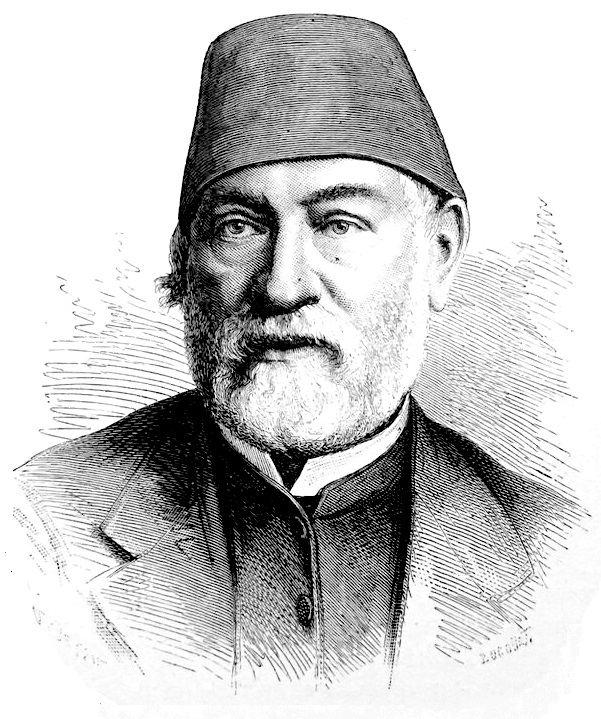
\includegraphics[height=12cm]{CoEg_Mariette_portrait.jpg}
\vfill
\hspace{0pt}

\pagebreak
\thispagestyle{empty}

\LARGE{C O R R E S P O N D A N C E S}
    
\Huge{É G Y P T O L O G I Q U E S}
\vspace{1\baselineskip}

\large C O N T E N A N T\space\space\space D E S
\vspace{1\baselineskip}

\Large L E T T R E S\space\space\space D ’ É G Y P T O L O G U E S
\vspace{2\baselineskip}

\large dispersées dans diverses institutions
\vspace{1\baselineskip}

et qui n’ont pas encore été rassemblées jusqu’à ce jour
\vspace{9\baselineskip}

\LARGE L E T T R E S\space\space\space D\space ’\space A U G .\space\space\space M A R I E T T E
\vspace{4\baselineskip}

\normalsize É D I T É E S\space\space\space P A R \space\space\space T H .\space\space\space L E B É E
\vspace{4\baselineskip}

Version 1,168
\vspace{1\baselineskip}

Octobre 2021
\end{titlepage}
\thispagestyle{empty}
\chapter*{Introduction}
\addcontentsline{toc}{chapter}{Introduction}
\setcounter{page}{1}

\section*{Le projet des \textit{Correspondances égyptologiques}}
\addcontentsline{toc}{section}{Le projet des Correspondances égyptologiques}

Ce fichier résulte d’un projet personnel d’édition numérique des lettres écrites par l’égyp-tologue Auguste Mariette. L’objectif de cette initiative est de rendre librement accessibles ces documents et de permettre leur exploitation scientifique.
\par Le corpus édité ici a vocation à intégrer chaque lettre repérée de Mariette. Les brouillons de lettres seront aussi incorporés, dans la mesure où il n’est pas toujours possible d’établir si une lettre a véritablement été transmise à son destinataire et que les hésitations et repentirs de la rédactions peuvent être riches d’enseignements.
\par L’édition des lettres sera progressive, afin de publier les documents régulièrement et d’en améliorer le format au moyen des suggestions qui pourront être recueillies au cours de l’entreprise. Les sources parisiennes seront dépouillées en priorité pour commencer, mais bien d’autres devraient suivre.
\par Les publications successives du corpus sont disponibles sur le site \href{https://thlebee.github.io/CoEg/}{\textit{Correspondances égyp}}-\href{https://thlebee.github.io/CoEg/}{\textit{tologiques}}, à la fois au format XML-TEI et en une version PDF réalisée au moyen de Latex (le présent fichier). Les métadonnées du corpus sont aussi disponibles. Chaque enrichissement sera signalé sur le carnet de recherche \href{https://hef.hypotheses.org/}{\textit{Histoire de l’égyptologie en formation}}.
\par Toute remarque, critique ou suggestion d’amélioration sera la bienvenue à l’adresse suivante~: \href{mailto:correspondances.egyptologiques@laposte.net}{correspondances.egyptologiques@laposte.net} (merci également d’y signaler toute utilisation qui pourra être faite de ces ressources, à titre d’information).
\par Le contenu de ce document est publié sous \href{https://creativecommons.org/licenses/by/4.0}{licence CC-BY}~: toute réutilisation en est permise, et encouragée~– sous réserve de la mention de la source~; par exemple~: «~Auguste Mariette (Thomas Lebée, éd.), \textit{Correspondances égyptologiques. Lettres d’Auguste Mariette}, lettre du 28 août 1853, d’Abousir, vraisemblablement à Nieuwerkerke (Archives nationales, 20150497, dossier 145 «~Mariette, Auguste~»)~».

\section*{Encodage et principes éditoriaux}
\addcontentsline{toc}{section}{Encodage et principes éditoriaux}

\par L’encodage résulte de plusieurs étapes, destinées à transcrire le document tel qu’il apparaît, puis à baliser ses composants structurels et un certain nombre de termes d’indexations.
\par Chaque lettre a été considérée comme une unité documentaire distincte, dont les réfé-rences bibliographiques et administratives sont rappelées en tête de notice, avec le cas échéant toute remarque jugée utile à sa compréhension. Les lettres peuvent dès lors être arrangées dans l’ordre chronologique pour retrouver leur continuité malgré la dispersion des fonds.
\par La ponctuation de Mariette a été conservée sans modification autant qu’elle était lisible. Pour être compréhensibles, les signes de ponctuation barrés ont parfois été remplacés par leur description entre crochets.
\par Cette édition recherche la plus grande fidélité au texte de Mariette. Les graphies variables des noms propres et l’absence d’accents sur les majuscules ont ainsi été conservées telles quelles. Les fautes d’orthographe, systématiques ou incidentes, ont également été respectées, et mar-quées par un balisage aproprié dès lors qu’elles s’éloignaient de l’orthographe et de l’usage contemporain. Toute intervention ou doute dans la lecture du texte manuscrit est signalée explicitement par le balisage ou la ponctuation.
\par Quand il existe des variantes causées par plusieurs versions d’une même lettre (par exemple un brouillon ou une copie), une des versions est choisie comme texte de base, dont les variantes sont indiquées en note, en circonscrivant les segments concernés. La notice des lettres concernées détaille alors la situation.
\par La copie numérique, comme la transcription par des caractères mécaniques, comporte cependant une part d’interprétation et de standardisation. Puisqu’il s’agissait de reproduire un texte manuscrit en caractères typographiques, les codes habituels ont été appliqués~: le texte souligné à la main a été rendu en italiques, le double soulignement par de petites capitales et les guillemets ont systématiquement été transcrits comme des guillemets typographiques (en chevrons).
\par L’écriture de Mariette n’est pas des plus régulières et les hampes de ses lettres sont parfois trompeuses. En cas de doute entre une majuscule ou une minuscule, ou même sur l’orthographe utilisée, la graphie régulière a été privilégiée en l’absence d’erreur manifeste. Les lectures hasardeuses sont signalées par le balisage, mais il est aussi à noter que les mots courts sont régulièrement de lecture délicate. Si le contexte permet d’en confirmer la plupart, certaines distinctions restent largement conjecturales (notamment la différence entre «~notre~»/ «~votre~» et «~nos~»/«~vos~»). Les ratures ont été déchiffrées dans la mesure du possible, ou juste indiquées en tant que telles.
\par Les marques postérieures à l’utilisation première des lettres (tampon de bibliothèque, foliotage, etc.) n’ont pas été reproduites. En revanche, les annotations portées sur les documents par leurs destinataires (annotation de secrétaire, indication de classement initial, etc.) sont indiquées dans la description de la lettre.

\section*{Le corpus}
\addcontentsline{toc}{section}{Le corpus}
\subsection*{Archives nationales}
\addcontentsline{toc}{subsection}{Archives nationales}

\hypertarget{CoEg_Mariette_ms_002}{}
\subsubsection*{F/17/2988/1, dossier « Mariette »}
\addcontentsline{toc}{subsubsection}{F/17/2988/1, dossier « Mariette »}
\begin{itemize}
\item (n. p.) \hyperlink{CoEg_Mariette_1846-04-13}{Le 13 avril 1846, de Boulogne-sur-Mer, au ministre de l’Instruction publique}~;
\item (n. p.) \hyperlink{CoEg_Mariette_1846-05-24}{Le 24 mai 1846, de Boulogne-sur-Mer, à Camaret, recteur de l’académie de Douai}~;
\item (n. p.) \hyperlink{CoEg_Mariette_1846-05-25}{Le 25 mai 1846, de Boulogne-sur-Mer, au ministre de l’Instruction publique}~;
\item (n. p.) \hyperlink{CoEg_Mariette_1846-09-29}{Le 29 septembre 1846, de Boulogne-sur-Mer, au ministre de l’Instruction publique}~;
\item (n. p.) \hyperlink{CoEg_Mariette_1850-05-20}{Le 20 mai 1850, de Paris, au ministre de l’Instruction publique}~;
\item (n. p.) \hyperlink{CoEg_Mariette_1850-07-06}{Le 6 juillet 1850, de Paris, au ministre de l’Instruction publique}~;
\item (n. p.) \hyperlink{CoEg_Mariette_1850-08-27}{Le 27 août 1850, de Paris, au ministre de l’Instruction publique}~;
\item (n. p.) \hyperlink{CoEg_Mariette_1851-10-14a}{Le 14 septembre 1851, de Saqqarah, à Le Moyne (copie)}~;
\item (n. p.) \hyperlink{CoEg_Mariette_1851-10-14b}{Le 14 septembre 1851, de Saqqarah, aux ministres de l'Intérieur et de l'Instruction publique (copie)}~;
\item (n. p.) \hyperlink{CoEg_Mariette_1855-01-26}{Le 26 janvier 1855, de Paris, au ministre de l’Instruction publique}~;
\item (n. p.) \hyperlink{CoEg_Mariette_1855-07-12}{Le 12 juillet 1855, de Paris, à un fonctionnaire de l’Instruction publique}~;
\item (n. p.) \hyperlink{CoEg_Mariette_1855-08-06}{Le 6 août 1855, de Paris, au ministre de l’Instruction publique}~;
\item (n. p.) \hyperlink{CoEg_Mariette_1855-12-12}{Le 12 décembre 1855, de Paris, à un fonctionnaire de l’Instruction publique}~;
\item (n. p.) \hyperlink{CoEg_Mariette_1856-02-11}{Le 11 février 1856, de Paris, au ministre de l’Instruction publique}~;
\item (n. p.) \hyperlink{CoEg_Mariette_1856-12-11}{Le 11 décembre 1856, de Paris, au ministre de l’Instruction publique}~;
\item (n. p.) \hyperlink{CoEg_Mariette_1856-12-31}{Le 31 décembre 1856, de Paris, au ministre de l’Instruction publique}~;
\item (n. p.) \hyperlink{CoEg_Mariette_1857-01-03}{Le 3 janvier 1857, de Paris, à un fonctionnaire de l’Instruction publique}~;
\item (n. p.) \hyperlink{CoEg_Mariette_1857-04-01}{Le 1\textsuperscript{er} avril 1857, de Paris, au ministre de l’Instruction publique}~;
\item (n. p.) \hyperlink{CoEg_Mariette_1857-08-26}{Le 26 août 1857, de Paris, à Servaux, chef du bureau des travaux historiques au ministère de l'Instruction publique}~;
\item (n. p.) \hyperlink{CoEg_Mariette_1857-10-04}{Le 4 octobre 1857, de Paris, au ministre de l’Instruction publique}~;
\item (n. p.) \hyperlink{CoEg_Mariette_1857-10-05}{Le 5 octobre 1857, de Paris, à un fonctionnaire de l’Instruction publique}~;
\item (n. p.) \hyperlink{CoEg_Mariette_1879-11-06}{Le 6 novembre 1879, de Paris, au président de la commission des missions scientifiques}.
\end{itemize}
\par Ces lettres ont été conservées dans le dossier qui rassemble les demandes de mission de Mariette\gls{CoEg_pers_00000001} au sein des archives du bureau des missions au ministère de l'Instruction publique\gls{CoEg_org_00000042}.
\par Les premières demandes, refusées, remontent à 1846, alors que Mariette\gls{CoEg_pers_00000001} enseignait au collège\gls{CoEg_org_00000029} de Boulogne-sur-Mer\gls{CoEg_place_00000035}. Il présenta des projets hardis qui ne convainquirent pas l'administration de lui confier une mission en Égypte\gls{CoEg_place_00000003}.
\par Il fut plus heureux en 1850, alors qu'il travaillait au Louvre\gls{CoEg_org_00000002} et avait fait connaissance avec le milieu égyptologique de la capitale\gls{CoEg_place_00000002}.
\par Les lettres qui suivent son retour en France, de 1855 à 1857, documentent ses projets de publication au sujet du \Gls{CoEg_entry_00000028}\gls{CoEg_place_00000004} de Memphis\gls{CoEg_place_00000005} et les missions qu'il entreprit dans cette optique aux musées de Londres\gls{CoEg_org_00000005}, Berlin\gls{CoEg_org_00000040} et Turin\gls{CoEg_place_00000021}.
\par En 1857, le nouveau projet qui occupa Mariette\gls{CoEg_pers_00000001} fut de retourner en Égypte\gls{CoEg_place_00000003} pour préparer le voyage (qui ne devait jamais se réaliser) du prince Napoléon\gls{CoEg_pers_00000074}. Ce fut l'occasion pour Mariette\gls{CoEg_pers_00000001} d'obtenir une mission gratuite qui, sans engager de dépense de la part du ministère\gls{CoEg_org_00000042}, plaçait son voyage préparatoire sous les auspices du gouvernement\gls{CoEg_org_00000012} et lui permettait de projeter une publication sur fonds publics à son retour. L'histoire devait en décider autrement.
\par Une dernière lettre est adressée en 1879 à la commission des missions scientifiques\gls{CoEg_org_00000039} (présidée par le ministre de l'Instruction publique) pour en solliciter le financement d'une publication portant sur les \glspl{CoEg_entry_00000027}.
\par La plupart de ces lettres sont destinées au ministre de l'Instruction publique. destinataire. Quelques-unes sont plus directement destinées à un fonctionnaire du ministère\gls{CoEg_org_00000042} ; il s'agit dans un cas d'Eugène Servaux\gls{CoEg_pers_00000237}, chef du bureau des travaux historiques.
\par Les dossiers de missions scientifiques du \textsc{xix}\textsuperscript{e} siècle ont été versés par le Centre national de la recherche scientifique aux Archives nationales\gls{CoEg_org_00000024} entre 1969 et 1973.

\hypertarget{CoEg_Mariette_ms_001}{}
\subsubsection*{20150497/118, dossier 145 « Mariette, Auguste »}
\addcontentsline{toc}{subsubsection}{20150497/118, dossier 145 « Mariette, Auguste »}
\noindent Ancienne cote : Paris, Bibliothèque centrale des musées nationaux, O/30/145 (cote utilisée avant le versement aux Archives nationales en 2015).
\begin{itemize}
\item (n. p.) \hyperlink{CoEg_Mariette_1849-10-20}{Le 20 octobre 1849, de Paris, à Longpérier}~;
\item (n. p.) \hyperlink{CoEg_Mariette_1850-07-08}{Le 8 juillet 1850, de Paris, à Nieuwerkerke}~;
\item (n. p.) \hyperlink{CoEg_Mariette_1851-02-28}{Le 28 février 1851, de Saqqarah, à Nieuwerkerke}~;
\item (n. p.) \hyperlink{CoEg_Mariette_1851-08-31}{Le 31 août 1851, de Saqqarah, à Nieuwerkerke}~;
\item (n. p.) \hyperlink{CoEg_Mariette_1851-09-14a}{Le 14 septembre 1851, de Saqqarah, à Le Moyne (copie)}~;
\item (n. p.) \hyperlink{CoEg_Mariette_1851-09-14b}{Le 14 septembre 1851, de Saqqarah, aux ministres de l’Intérieur et de l’Instruction publique (copie)}~;
\item (n. p.) \hyperlink{CoEg_Mariette_1852-01-16}{Le 16 janvier 1852, d’Abousir, vraisemblablement à Nieuwerkerke}~;
\item (n. p.) \hyperlink{CoEg_Mariette_1852-08-04}{Le 4 août 1852, d’Abousir, vraisemblablement à Nieuwerkerke}~;
\item (n. p.) \hyperlink{CoEg_Mariette_1852-08-20}{Le 20 août 1852, d’Abousir, au ministre de l'Intérieur}~;
\item (n. p.) \hyperlink{CoEg_Mariette_1852-09-03}{Le 3 septembre 1852, d’Abousir, au ministre de l'Intérieur}~;
\item (n. p.) \hyperlink{CoEg_Mariette_1852-09-04}{Le 4 septembre 1852, d’Abousir, vraisemblablement à Nieuwerkerke}~;
\item (n. p.) \hyperlink{CoEg_Mariette_1852-11-12}{Le 12 novembre 1852, d’Abousir, vraisemblablement à Nieuwerkerke}~;
\item (n. p.) \hyperlink{CoEg_Mariette_1852-12-28}{Le 28 décembre 1852, d’Abousir, au ministre de l'Intérieur}~;
\item (n. p.) \hyperlink{CoEg_Mariette_1853-01-01}{Le 1\textsuperscript{er} janvier 1853, d’Abousir, vraisemblablement à Nieuwerkerke}~;
\item (n. p.) \hyperlink{CoEg_Mariette_1853-05-06}{Le 6 mai 1853, d’Abousir, à Nieuwerkerke}~;
\item (n. p.) \hyperlink{CoEg_Mariette_1853-07-30}{Le 30 juillet 1853, du Caire, à Nieuwerkerke}~;
\item (n. p.) \hyperlink{CoEg_Mariette_1853-08-10}{Le 10 août 1853, d’Abousir, vraisemblablement à Nieuwerkerke}~;
\item (n. p.) \hyperlink{CoEg_Mariette_1853-08-28}{Le 28 août 1853, d’Abousir, vraisemblablement à Nieuwerkerke}~;
\item (n. p.) \hyperlink{CoEg_Mariette_1857-02-20}{Le 20 février 1857, de Paris, à Nieuwerkerke}~;
\item (n. p.) \hyperlink{CoEg_Mariette_1857-10-26}{Le 26 octobre 1857, d’Alexandrie, à Nieuwerkerke}~;
\item (n. p.) \hyperlink{CoEg_Mariette_1857-11-29}{Le 29 novembre 1857, d’Assiout, à Nieuwerkerke}~;
\item (n. p.) \hyperlink{CoEg_Mariette_1858-01-23}{Le 23 janvier 1858, du Caire, à Nieuwerkerke}~;
\item (n. p.) \hyperlink{CoEg_Mariette_1860-12-20}{Le 20 décembre 1860, de Boulaq, à Nieuwerkerke}~;
\item (n. p.) \hyperlink{CoEg_Mariette_1867-04-13}{Le 13 avril 1867, de Paris, à Nieuwerkerke}.
\end{itemize}
\par Ces lettres ont été conservées dans le dossier personnel de Mariette\gls{CoEg_pers_00000001} au sein des archives de l’administration des musées nationaux\gls{CoEg_org_00000001}. Elles correspondent à plusieurs étapes de sa carrière. Malgré leur cordialité de ton et quelques anecdotes, il s’agit surtout d’une correspondance professionnelle, dans laquelle l’égyptologue évoque à sa hiérarchie les progrès de ses missions et ses préoccupations en ce qui concerne l’entretien matériel de sa famille.
\par La première lettre correspond à ses débuts au Louvre\gls{CoEg_org_00000002} ; il y demande l’autorisation (qui ne semble pas lui avoir été accordée) d’améliorer son traitement en accomplissant des petits travaux sur les papyrus du musée en dehors de ses heures de service.
\par Les dix-sept lettres suivantes datent de son premier voyage en Égypte\gls{CoEg_place_00000003} (1850-1853). Il y informe sa hiérarchie de la situation du terrain, réclame périodiquement des fonds et demande des directives ou explique ses initiatives. Les négociations avec le gouvernement égyptien\gls{CoEg_org_00000008}, les stratagèmes de Mariette\gls{CoEg_pers_00000001} pour interpréter très libéralement les accords conclus avec celui-ci (ou le contourner tout à fait) et la coordination de ses efforts avec ceux du ministère des Affaires étrangères\gls{CoEg_org_00000007}, par le truchement du consulat général\gls{CoEg_org_00000006} de France\gls{CoEg_org_00000012} à Alexandrie\gls{CoEg_place_00000006} sont les principaux objets de ces lettres, qui renferment également des indications précises sur l’avancée des fouilles et quelques détails de sa vie quotidienne.
\par La lettre suivante date de 1857~; Mariette\gls{CoEg_pers_00000001} y demande un congé pour accomplir une mission au musée égyptien de Turin\gls{CoEg_org_00000021}.
\par Les trois lettres qui suivent datent du second voyage de Mariette\gls{CoEg_pers_00000001} en Égypte\gls{CoEg_place_00000003} (1857-1858). Elles traitent surtout de la préparation du voyage du prince Napoléon\gls{CoEg_pers_00000074} (qui n’eut finalement pas lieu avant 1863, mais constituait le prétexte officiel à cette nouvelle mission)~; de l’annonce par Mariette\gls{CoEg_pers_00000001} d’acquisitions destinées au prince, mais dont il espère qu’elles rejoindront le Louvre\gls{CoEg_org_00000002}~; et enfin de la préoccupation de l’organisation de ses congés, pour lui permettre de rester éloigné du Louvre\gls{CoEg_org_00000002} sans déroger au règlement et permettre à sa famille de toucher ses appointements.
\par La lettre suivante, du 20 décembre 1860, est la réponse d’une lettre envoyée à Mariette\gls{CoEg_pers_00000001} par Nieuwerkerke\gls{CoEg_pers_00000002} le 29 novembre (conservée dans le dossier et transcrite en note) et dans laquelle il lui annonçait être contraint de nommer un conservateur adjoint à sa place, et le nommait lui-même conservateur adjoint honoraire. Mariette\gls{CoEg_pers_00000001} se trouvait alors déjà engagé au service du vice-roi\gls{CoEg_pers_00000080} d’Égypte\gls{CoEg_place_00000003} pour diriger le service des antiquités.
\par Enfin, la dernière lettre de cette série date de 1867~: alors commissaire du pavillon égyptien à l'Exposition universelle de Paris\gls{CoEg_place_00000002}, Mariette\gls{CoEg_pers_00000001} demande à Nieuwerkerke\gls{CoEg_pers_00000002} de l’excuser de n’avoir pas reçu une invitation égarée.
\par Toutes ces lettres s’adressent à la hiérarchie de Mariette\gls{CoEg_pers_00000001} à différents moments de sa car-rière~: Adrien de Longpérier\gls{CoEg_pers_00000033}\footnote{Supérieur de Mariette\gls{CoEg_pers_00000001} en 1849 en tant que conservateur du département des sculptures et des antiques\gls{CoEg_org_00000025} du musée du Louvre\gls{CoEg_org_00000002} (le département égyptien\gls{CoEg_org_00000020} venait tout juste de recevoir un conservateur propre avec la nomination de Rougé\gls{CoEg_pers_00000032} le 1\textsuperscript{er} août 1849).}~; les ministres responsables de sa première mission\footnote{Le ministre de l’Intérieur (dont dépendaient les musées nationaux\gls{CoEg_org_00000001} jusqu’en 1853) et celui de l’Instruction publique.}~; sept lettres s’adressent explicitement au directeur du musée du Louvre\gls{CoEg_org_00000002}, le comte de Nieuwerkerke\gls{CoEg_pers_00000002}. Le destinataire de neuf de ces lettres n’est pas nommé~; il s’agissait manifestement d’un haut fonctionnaire parisien en relation avec les autres administrations et qui fréquentait les collègues de Mariette\gls{CoEg_pers_00000001} au Louvre\gls{CoEg_org_00000002}, distinct cependant du vicomte de Rougé\gls{CoEg_pers_00000032} qui est évoqué à la troisième personne~: il est très probable qu’il s’agisse là aussi du comte de Nieuwerkerke\gls{CoEg_pers_00000002}.
\par Les brouillons de plusieurs de ces lettres sont conservés à la Bibliothèque nationale de France\gls{CoEg_org_00000026} sous la cote ms. NAF 20179.
\par Ces documents ont été rassemblés assez tôt au sein des archives du Louvre\gls{CoEg_org_00000002}, où il semble que douze des lettres écrites par Mariette\gls{CoEg_pers_00000001} pendant sa première mission ont été copiées. Cette copie n'est pas datée ni signée~; l’écriture est ancienne mais ne correspond ni à la main de Mariette\gls{CoEg_pers_00000001}, ni à celle de Maspero, et le copiste n’était pas familier des noms propres égyptiens. Ces copies, avec d’autres, sont aujourd’hui conservées à la bibliothèque de l’Institut de France\gls{CoEg_org_00000004} sous la cote ms. 4061 (2), f\textsuperscript{os} 11-57.
\par Les archives conservées à la bibliothèque centrale des musées nationaux ont été versées aux Archives nationales\gls{CoEg_org_00000024} en 2015.

\subsection*{Bibliothèque de l'Institut de France}
\addcontentsline{toc}{subsection}{Bibliothèque de l'Institut de France}

\hypertarget{CoEg_Mariette_ms_004}{}
\subsubsection*{Ms. 2572-2588}
\addcontentsline{toc}{subsubsection}{Ms. 2572-2588}

\begin{itemize}
\item (f\textsuperscript{os} 270-272) \hyperlink{CoEg_Mariette_1857-03-25}{Le 25 mars 1857, de Paris, à Chabas} ;
\item (f\textsuperscript{os} 270-273) \hyperlink{CoEg_Mariette_1860-02-01}{Le 1\textsuperscript{er} février 1860, de Louqsor, à Chabas} ;
\item (f\textsuperscript{os} 661-664) \hyperlink{CoEg_Mariette_1862-04-07}{Le 7 avril 1862, de Boulogne-sur-Mer, à Chabas} ;
\item (f\textsuperscript{os} 767-770) \hyperlink{CoEg_Mariette_1862-10-09}{Le 9 octobre 1862, de Paris, à Chabas} ;
\item (f\textsuperscript{os} 321-324) \hyperlink{CoEg_Mariette_1870-06-23}{Le 23 juin 1870, du Caire, à Chabas} ;
\item (f\textsuperscript{os} 845-852) \hyperlink{CoEg_Mariette_1871-08-30}{Le 30 août 1871, de Paris, à Chabas} ;
\item (f\textsuperscript{os} 921-924) \hyperlink{CoEg_Mariette_1871-09-15}{Le 15 septembre 1871, de Paris, à Chabas} ;
\item (f\textsuperscript{os} 255-258) \hyperlink{CoEg_Mariette_1872-04-13}{Le 13 avril 1872, sans lieu indiqué, à Chabas} ;
\item (f\textsuperscript{os} 315-320) \hyperlink{CoEg_Mariette_1872-05-05}{Le 5 mai 1872, de Boulaq, à Chabas} ;
\item (f\textsuperscript{os} 443-446) \hyperlink{CoEg_Mariette_1872-07-03}{Le 3 juillet 1872, de Paris, à Chabas} ;
\item (f\textsuperscript{os} 619-622) \hyperlink{CoEg_Mariette_1872-09-15}{Le 15 septembre 1872, de Paris, à Chabas} ;
\item (f\textsuperscript{os} 694-697) \hyperlink{CoEg_Mariette_1872-10-06}{Le 6 octobre 1872, de Paris, à Chabas} ;
\item (f\textsuperscript{os} 28-31) \hyperlink{CoEg_Mariette_1873-01-05}{Le 5 janvier 1873, de Boulaq, à Chabas} ;
\item (f\textsuperscript{os} 182-185) \hyperlink{CoEg_Mariette_1873-02-23a}{Le 23 février 1873, de Boulaq, à Chabas} ;
\item (f\textsuperscript{os} 296-299) \hyperlink{CoEg_Mariette_1873-04-23}{Le 23 avril 1873, de Boulogne-sur-Mer, à Chabas} ;
\item (f\textsuperscript{os} 527-530) \hyperlink{CoEg_Mariette_1873-08-16c}{Le 16 août 1873, de Pont-de-Briques, à Chabas} ;
\item (f\textsuperscript{os} 758-761) \hyperlink{CoEg_Mariette_1873-11-01}{Le 1\textsuperscript{er} novembre 1873, de Boulaq, à Chabas} ;
\item (f\textsuperscript{os} 321-324) \hyperlink{CoEg_Mariette_1874-04-29}{Le 29 avril 1874, du Caire, à Chabas} ;
\item (f\textsuperscript{os} 603-606) \hyperlink{CoEg_Mariette_1875-07-18}{Le 18 juillet 1875, de Boulogne-sur-Mer, à Chabas} ;
\item (f\textsuperscript{os} 381-384) \hyperlink{CoEg_Mariette_1876-07-21}{Le 21 juillet 1876, de Point-de-Briques, à Chabas} ;
\item (f\textsuperscript{os} 324-327) \hyperlink{CoEg_Mariette_1877-05-18}{Le 18 mai 1877, de Pont-de-Briques, à Chabas}.
\end{itemize}

\par Ces vingt-et-une lettres ont été conservées par Chabas lui-même dans les recueils qu’il constituait avec sa correspondance, classés par ordre chronologique et indexés par interlocuteur, matière et terme égyptien. 
Les échanges entre Chabas et Mariette commencèrent relativement tôt dans la carrière de celui-ci puisque la première lettre envoyée de l’un à l’autre date de 1855 \footnote{Chabas y remercie Mariette de lui avoir envoyé une de ses publications – manifestement un tirage à part des «~Renseignements sur les soixante-quatre Apis trouvés dans les souterrains du Sérapéum~» qu’il avait fait publier dans le \textit{Bulletin archéologique de l’Athénæum français} – (ms.~2572, p.~109-112).}. Dans la première lettre de Mariette à Chabas conservée, ce dernier sert de truchement à Samuel Birch pour s’enquérir de l’acceptation d’un mémoire sur les coupes de Djéhouty présenté à la Société des antiquaires.
\par C’est après l’entrée de Mariette au service du vice-roi d’Égypte que ses échanges avec Chabas semblent devenir plus réguliers, même s’ils restent épisodiques. Mariette semble tenir à se rendre utile à Chabas qu’il regarde comme un maître de l’égyptologie française.
\par Aucune lettre n’a été conservée entre 1862 et 1870~: il s’agit d’un refroidissement malheureux des relations entre les deux hommes, causé par la crise occasionnée en 1865 par la publication sauvage par Dümichen et Lepsius d’une stèle découverte par Mariette, dénoncées par Ernest Desjardins à la demande de celui-ci mais en termes outranciers qui polarisèrent les égyptologues et suscitèrent en retour des reproches douloureux mais justifiés sur la lenteur avec laquelle Mariette faisait connaître les monuments exhumés d’Égypte, dont il décourageait manifestement toute autre publication. La réconciliation eut lieu grâce à l’intermédiaire d’amis communs et porta ses fruits en 1870 \footnote{\textsc{Maspero} Gaston, «~Auguste Mariette (1821-1881). Notice biographique~», dans \textsc{Mariette} Auguste (\textsc{Maspero} Gaston, éd.), \textit{Œuvres diverses} 1 (\textit{Bibliothèque égyptologique} 18), Paris, Leroux, 1904, p. I-CCXXIV, p. \href{https://digi.ub.uni-heidelberg.de/diglit/mariette1904bd1/0166}{CL} et \href{https://digi.ub.uni-heidelberg.de/diglit/mariette1904bd1/0191}{CLXXV} ; \textsc{Maspero} Gaston, «~Auguste Mariette (1821-1881). Notice biographique~», dans \textsc{Chabas} François (\textsc{Maspero} Gaston, éd.), \textit{Œuvres diverses} 1 (\textit{Bibliothèque égyptologique} 9), Paris, Leroux, 1899, p. I-CLII, p. \href{https://gallica.bnf.fr/ark:/12148/bpt6k555357/f117}{CVII}.}.
\par La première moitié des années 1870 voit leurs échanges les plus réguliers, avec trois à quatre lettres de Mariette conservées par an. Ces communications sont notamment stimulées par la question de la validité des silex taillés comme preuve de l’existence d’une préhistoire égyptienne. Le rythme de la correspondance diminue ensuite sans qu’il soit possible de savoir s’il s’agit d’un ralentissement effectif de leurs échanges ou d’une conservation plus partielle des lettres de ces dernières années.
Aussi riche que soit cet ensemble, il semble en effet qu’il comporte quelques lacunes : Chabas n’a en effet pas joint de minute de toutes les lettres qu’il adressait à ses correspondants (seules six en sont conservées pour Mariette, contre vingt-et-une lettres reçues de lui) ; inversement, il semble parfois manquer des lettres intermédiaires que Chabas a dû recevoir (il semble ainsi anormal de n’avoir qu’une lettre pour 1860-1861, et environ une lettre par an entre 1873 et 1877, qui sont trop brèves pour résumer leurs échanges du moment), sans qu’il soit désormais possible d’établir si ces lettres ne justifiaient pas par leur contenu d’être conservées.
\par Chabas n’eut pas le temps de relier et d’organiser le dernier volume de sa correspondance scientifique, qui recouvre les années 1878-1882. Les recueils passèrent alors en possession de sa fille, Mme Piquemal-Chabas et quittèrent Chalon-sur-Saône à une date indéterminée ; ils se trouvaient chez elle, à Paris, quand elle en fit don à l’Académie des inscriptions et belles-lettres en 1915\footnote{Le don est formellement accepté au cours de la séance du 4 juin 1915 (\textit{Comptes rendus des séances de l’Académie des inscriptions et belles-lettres} 59-3, 1915, p. \href{https://www.persee.fr/doc/crai_0065-0536_1915_num_59_3_73560}{224-225}). Maspero y avait recouru pour les introductions biographiques de la Bibliothèque égyptologique, et il passait par l’intermédiaire de M\textsuperscript{me} Piquemal-Chabas pour vérifier un détail qui s’y trouvait en 1907 ; quelques jours après l’acceptation du don par l’Académie en séance, elle lui fit savoir qu’on pouvait venir chercher les recueils chez elle à Paris (bibliothèque de l’Institut de France, ms. 4036, fos 134-140).}. Elles sont depuis conservées à la bibliothèque de l’Institut de France sous la cote ms. 2572-2588.

\subsection*{Bibliothèque nationale de France}
\addcontentsline{toc}{subsection}{Bibliothèque nationale de France}

\hypertarget{CoEg_Mariette_ms_003}{}
\subsubsection*{NAF 11669}
\addcontentsline{toc}{subsubsection}{NAF 11669}

\begin{itemize}
\item (f\textsuperscript{o} 189) \hyperlink{CoEg_Mariette_18xx-xx-xx_ms003f189}{Vraisemblablement entre février 1848 et juin 1849, sans lieu, à Jeanron, directeur général des musées nationaux}~;
\item (f\textsuperscript{os} 2-3) \hyperlink{CoEg_Mariette_1860-08-12}{Le 12 août 1860, du Caire, à Desjardins} ;
\item (f\textsuperscript{o} 4) \hyperlink{CoEg_Mariette_1862-02-28}{Le 28 février 1862, du Caire, à Desjardins} ;
\item (f\textsuperscript{os} 5-6) \hyperlink{CoEg_Mariette_1862-07-18}{Le 18 juillet 1862, de Boulogne-sur-Mer, à Desjardins} ;
\item (f\textsuperscript{os} 7-8) \hyperlink{CoEg_Mariette_1862-09-16}{Le 16 septembre 1862, de Boulogne-sur-Mer, à Desjardins} ;
\item (f\textsuperscript{os} 9-10) \hyperlink{CoEg_Mariette_1863-03-03}{Le 3 mars 1863, de Boulaq, à Desjardins} ;
\item (f\textsuperscript{os} 11-12) \hyperlink{CoEg_Mariette_1863-04-03}{Le 3 avril 1863, de Boulaq, à Desjardins} ;
\item (f\textsuperscript{os} 13-14) \hyperlink{CoEg_Mariette_1863-06-16}{Le 16 juin 1863, de Boulaq, à Desjardins} ;
\item (f\textsuperscript{os} 15-16) \hyperlink{CoEg_Mariette_1863-08-08}{Le 8 août 1863, de Le Caire, à Desjardins} ;
\item (f\textsuperscript{os} 17-18) \hyperlink{CoEg_Mariette_1864-04-16}{Le 16 avril 1864, de Boulaq, à Desjardins} ;
\item (f\textsuperscript{os} 22-24) \hyperlink{CoEg_Mariette_1865-01-07}{Le 7 janvier 1865, de Boulaq, à Desjardins} ;
\item (f\textsuperscript{o} 25) \hyperlink{CoEg_Mariette_1865-09-09}{Le 9 septembre 1865, du Caire, à Desjardins} ;
\item (f\textsuperscript{o} 26) \hyperlink{CoEg_Mariette_1865-10-27}{Le 27 octobre 1865, du Caire, à Desjardins} ;
\item (f\textsuperscript{o} 27) \hyperlink{CoEg_Mariette_1867-01-10}{Le 10 janvier 1867, de Paris, à Desjardins} ;
\item (f\textsuperscript{o} 28) \hyperlink{CoEg_Mariette_1867-xx-xxms003f28}{En 1867 et de Paris, à Desjardins} ;
\item (f\textsuperscript{o} 29) \hyperlink{CoEg_Mariette_1867-01-18}{Le 18 janvier 1867, de Paris ou Auteuil, à Desjardins} ;
\item (f\textsuperscript{os} 30-31) \hyperlink{CoEg_Mariette_1867-03-11}{Le 11 mars 1867, de Paris, à Desjardins} ;
\item (f\textsuperscript{o} 32) \hyperlink{CoEg_Mariette_1867-xx-xx_ms003f32}{En 1867, de Paris, à Desjardins} ;
\item (f\textsuperscript{o} 33) \hyperlink{CoEg_Mariette_1867-xx-xx_ms003f33}{En 1867, de Paris, à Desjardins} ;
\item (f\textsuperscript{o} 34) \hyperlink{CoEg_Mariette_1867-xx-xx_ms003f34}{En 1867, sans lieu, à Desjardins} ;
\item (f\textsuperscript{o} 35) \hyperlink{CoEg_Mariette_1867-xx-xx_ms003f35}{En 1867, sans lieu, à Desjardins} ;
\item (f\textsuperscript{o} 36) \hyperlink{CoEg_Mariette_1867-xx-xx_ms003f36}{En 1867, de Paris, à Desjardins} ;
\item (f\textsuperscript{o} 37) \hyperlink{CoEg_Mariette_1867-xx-xx_ms003f37}{En 1867, sans lieu, à Desjardins} ;
\item (f\textsuperscript{o} 38) \hyperlink{CoEg_Mariette_1867-xx-xx_ms003f38}{En 1867, sans lieu, à Desjardins} ;
\item (f\textsuperscript{o} 39) \hyperlink{CoEg_Mariette_1867-04-xx_ms003f41}{En 1867, sans lieu, à Desjardins} ;
\item (f\textsuperscript{o} 41) \hyperlink{CoEg_Mariette_1867-xx-xx_ms003f39}{En avril ou mai 1867, sans lieu, à Desjardins} ;
\item (f\textsuperscript{o} 42) \hyperlink{CoEg_Mariette_1867-xx-xx_ms003f42}{En 1867, sans lieu, à Desjardins} ;
\item (f\textsuperscript{os} 51-52) \hyperlink{CoEg_Mariette_186x-xx-xx_ms003f51-52}{Peut-être en 1867, sans lieu, à Desjardins} ;
\item (f\textsuperscript{os} 43-44) \hyperlink{CoEg_Mariette_1868-01-04}{Le 4 janvier 1868, du Caire, à Desjardins} ;
\item (f\textsuperscript{os} 45-46) \hyperlink{CoEg_Mariette_1868-03-07}{Le 7 mars 1868, de Boulaq, à Desjardins} ;
\item (f\textsuperscript{os} 47-48) \hyperlink{CoEg_Mariette_1868-05-08}{Le 8 mai 1868, du Caire, à Desjardins} ;
\item (f\textsuperscript{os} 49-50) \hyperlink{CoEg_Mariette_1868-05-18}{Le 18 mai 1868, de Boulaq, à Desjardins} ;
\item (f\textsuperscript{os} 53-55) \hyperlink{CoEg_Mariette_1868-10-29}{Le 29 octobre 1868, de Boulaq, à Desjardins} ;
\item (f\textsuperscript{os} 56-57) \hyperlink{CoEg_Mariette_1868-12-17}{Le 17 décembre 1868, d'Edfou, à Desjardins} ;
\item (f\textsuperscript{os} 63-64) \hyperlink{CoEg_Mariette_1869-02-02}{Le 2 février 1869, de Boulaq, à Desjardins} ;
\item (f\textsuperscript{os} 65-66) \hyperlink{CoEg_Mariette_1869-02-03}{Le 3 février 1869, de Boulaq, à Desjardins} ;
\item (f\textsuperscript{os} 67-68) \hyperlink{CoEg_Mariette_1869-05-10}{Le 10 mai 1869, de Saqqarah, à Desjardins} ;
\item (f\textsuperscript{o} 69) \hyperlink{CoEg_Mariette_1869-06-20}{Peut-être le 20 juin 1869, sans lieu, à Desjardins} ;
\item (f\textsuperscript{o} 58) \hyperlink{CoEg_Mariette_1869-07-xx}{Juillet 1869, de Paris, à Desjardins} ;
\item (f\textsuperscript{o} 60) \hyperlink{CoEg_Mariette_1869-08-10}{Le 10 août 1869, de Plombière, à Desjardins} ;
\item (f\textsuperscript{o} 61) \hyperlink{CoEg_Mariette_1869-08-18}{Sans doute le 18 août 1869, de Paris, à Desjardins} ;
\item (f\textsuperscript{os} 70-71) \hyperlink{CoEg_Mariette_1869-10-25}{Le 25 octobre 1869, de Boulaq, à Desjardins} ;
\item (f\textsuperscript{os} 72-73) \hyperlink{CoEg_Mariette_1869-12-06}{Le 6 décembre 1869, de Boulaq, à Desjardins} ;
\item (f\textsuperscript{os} 74-75) \hyperlink{CoEg_Mariette_1870-01-28}{Le 28 janvier 1870, de Boulaq, à Desjardins} ;
\item (f\textsuperscript{os} 78-80) \hyperlink{CoEg_Mariette_1870-03-18}{Le 18 mars 1870, de Boulaq, à Desjardins} ;
\item (f\textsuperscript{os} 76-77) \hyperlink{CoEg_Mariette_1870-04-27}{Le 27 avril 1870, de Boulaq, à Desjardins} ;
\item (f\textsuperscript{o} 81) \hyperlink{CoEg_Mariette_1870-06-21}{Le 21 juin 1870, du Caire, à Desjardins} ;
\item (f\textsuperscript{os} 82-83) \hyperlink{CoEg_Mariette_1871-xx-xx_ms003f82-83}{En 1871, sans doute de Paris, à Desjardins} ;
\item (f\textsuperscript{os} 84-85) \hyperlink{CoEg_Mariette_18xx-xx-xx_ms003f84-85}{Sans date ni lieu, à Desjardins} ;
\item (f\textsuperscript{os} 86-87) \hyperlink{CoEg_Mariette_1872-10-21}{Le 21 octobre 1872, de Boulaq, à Desjardins} ;
\item (f\textsuperscript{os} 88-90) \hyperlink{CoEg_Mariette_1873-02-23b}{Le 23 février 1873, de Boulaq, à Desjardins} ;
\item (f\textsuperscript{os} 91-92) \hyperlink{CoEg_Mariette_1873-03-17}{Le 17 mars 1873, de Boulaq, à Desjardins} ;
\item (f\textsuperscript{os} 93) \hyperlink{CoEg_Mariette_1873-03-28}{Le 28 mars 1873, sans lieu, à Desjardins} ;
\item (f\textsuperscript{os} 94-95) \hyperlink{CoEg_Mariette_1873-06-22}{Le 22 juin 1873, de Vienne, à Desjardins} ;
\item (f\textsuperscript{os} 96-97) \hyperlink{CoEg_Mariette_1873-06-24}{Le 24 juin 1873, de Vienne, à Desjardins} ;
\item (f\textsuperscript{os} 98) \hyperlink{CoEg_Mariette_18xx-xx-xx_ms003f98}{Sans date ni lieu, à Desjardins} ;
\item (f\textsuperscript{os} 99) \hyperlink{CoEg_Mariette_18xx-xx-xx_ms003f99}{Sans date ni lieu, à Desjardins} ;
\item (f\textsuperscript{os} 100-101) \hyperlink{CoEg_Mariette_1873-08-06}{Le 6 août 1873, de Pont-de-Briques, à Desjardins} ;
\item (f\textsuperscript{os} 102-103) \hyperlink{CoEg_Mariette_1873-08-16a}{Le 16 août 1873, de Pont-de-Briques, à Desjardins} ;
\item (f\textsuperscript{os} 104-105) \hyperlink{CoEg_Mariette_1873-08-16b}{Le 16 août 1873, de Pont-de-Briques, à Dubief} ;
\item (f\textsuperscript{os} 107-108) \hyperlink{CoEg_Mariette_1873-08-20}{Le 20 août 1873, de Pont-de-Briques, à Desjardins} ;
\item (f\textsuperscript{os} 109-110) \hyperlink{CoEg_Mariette_1873-09-23}{Le 23 septembre 1873, de Pont-de-Briques, à Desjardins} ;
\item (f\textsuperscript{os} 111-112) \hyperlink{CoEg_Mariette_1873-11-16}{Le 16 novembre 1873, du Caire, à Desjardins} ;
\item (f\textsuperscript{os} 113-114) \hyperlink{CoEg_Mariette_1873-12-21}{Le 21 décembre 1873, de Boulaq, à Desjardins} ;
\item (f\textsuperscript{os} 115-118) \hyperlink{CoEg_Mariette_1874-03-30}{Le 30 mars 1874, de Boulaq, à Desjardins} ;
\item (f\textsuperscript{os} 119) \hyperlink{CoEg_Mariette_xxxx-xx-xx_ms003f119}{Peut-être en 1874, vraisemblablement de Paris, à Desjardins} ;
\item (f\textsuperscript{os} 123-124) \hyperlink{CoEg_Mariette_1874-08-15}{Le 15 août 1874, de Pont-de-Briques, à Desjardins} ;
\item (f\textsuperscript{os} 120-122) \hyperlink{CoEg_Mariette_1874-08-17}{Le 17 août 1874, de Pont-de-Briques, à Desjardins} ;
\item (f\textsuperscript{os} 125-126) \hyperlink{CoEg_Mariette_1875-07-12}{Le 12 juillet 1875, de Boulogne-sur-Mer, à Desjardins} ;
\item (f\textsuperscript{os} 127-130) \hyperlink{CoEg_Mariette_1876-04-30}{Le 30 avril 1876, de Boulogne-sur-Mer, à Desjardins} ;
\item (f\textsuperscript{os} 131) \hyperlink{CoEg_Mariette_1876-07-02}{Le 2 juillet 1876, de Pont-de-Briques, à Desjardins} ;
\item (f\textsuperscript{os} 132-133) \hyperlink{CoEg_Mariette_1876-07-05}{Le 5 juillet 1876, de Pont-de-Briques, à Desjardins} ;
\item (f\textsuperscript{os} 134-135) \hyperlink{CoEg_Mariette_1876-07-19}{Le 19 juillet 1876, de Pont-de-Briques, à Desjardins} ;
\item (f\textsuperscript{os} 136) \hyperlink{CoEg_Mariette_1876-08-02}{Le 2 août 1876, de Pont-de-Briques, à Desjardins} ;
\item (f\textsuperscript{os} 137-138) \hyperlink{CoEg_Mariette_1876-08-29}{Le 29 août 1876, de Pont-de-Briques, à Desjardins} ;
\item (f\textsuperscript{os} 139-140) \hyperlink{CoEg_Mariette_1876-09-16}{Le 16 septembre 1876, de Pont-de-Briques, à Desjardins} ;
\item (f\textsuperscript{os} 141-142) \hyperlink{CoEg_Mariette_18xx-xx-xx_ms003f141-142}{Sans date, de Boulogne-sur-Mer, à Desjardins} ;
\item (f\textsuperscript{os} 143-144) \hyperlink{CoEg_Mariette_1879-05-02}{Le 2 mai 1879, de Boulaq, à Desjardins} ;
\item (f\textsuperscript{os} 145) \hyperlink{CoEg_Mariette_1879-05-05}{Le 5 mai 1879, sans doute de Boulaq, à Desjardins} ;
\item (f\textsuperscript{os} 146-147) \hyperlink{CoEg_Mariette_1879-05-08}{Le 8 mai 1879, de Boulaq, à Desjardins} ;
\item (f\textsuperscript{os} 148-149) \hyperlink{CoEg_Mariette_1879-05-10}{Le 10 mai 1879, sans doute de Boulaq, à Desjardins} ;
\item (f\textsuperscript{os} 150-151) \hyperlink{CoEg_Mariette_1879-06-20}{Le 20 juin 1879, de Boulogne-sur-Mer, à Desjardins} ;
\item (f\textsuperscript{os} 152) \hyperlink{CoEg_Mariette_1879-06-25}{Le 25 juin 1879, de Boulogne-sur-Mer, à Desjardins} ;
\item (f\textsuperscript{os} 153-154) \hyperlink{CoEg_Mariette_1879-09-21}{Le 21 septembre 1879, de Boulogne-sur-Mer, à Desjardins} ;
\item (f\textsuperscript{os} 155-156) \hyperlink{CoEg_Mariette_1879-10-01}{Le 1\textsuperscript{er} octobre 1879, de Boulogne-sur-Mer, à Desjardins} ;
\item (f\textsuperscript{os} 157) \hyperlink{CoEg_Mariette_1879-10-07}{Le 7 octobre 1879, de Boulogne-sur-Mer, à Desjardins} ;
\item (f\textsuperscript{os} 158) \hyperlink{CoEg_Mariette_1879-10-12}{Le 12 octobre 1879, de Boulogne-sur-Mer, à Desjardins} ;
\item (f\textsuperscript{os} 159-161) \hyperlink{CoEg_Mariette_1879-10-21}{Le 21 octobre 1879, de Boulogne-sur-Mer, à Desjardins} ;
\item (f\textsuperscript{os} 162-164) \hyperlink{CoEg_Mariette_1879-10-22}{Le 22 octobre 1879, de Boulogne-sur-Mer, à Desjardins} ;
\item (f\textsuperscript{os} 165-166) \hyperlink{CoEg_Mariette_1879-10-25}{Le 25 octobre 1879, de Boulogne-sur-Mer, à Desjardins} ;
\item (f\textsuperscript{os} 167) \hyperlink{CoEg_Mariette_1879-11-02}{Le 2 novembre 1879, de Boulogne-sur-Mer, à Desjardins} ;
\item (f\textsuperscript{os} 168) \hyperlink{CoEg_Mariette_1879-11-12}{Le 12 novembre 1879, de Boulogne-sur-Mer, à Desjardins} ;
\item (f\textsuperscript{os} 169) \hyperlink{CoEg_Mariette_1879-11-19}{Le 19 novembre 1879, de Paris, à Desjardins} ;
\item (f\textsuperscript{os} 170-172) \hyperlink{CoEg_Mariette_1879-12-27}{Le 27 décembre 1879, de Boulaq, à Desjardins} ;
\item (f\textsuperscript{os} 173-174) \hyperlink{CoEg_Mariette_1880-01-14}{Le 14 janvier 1880, de Boulaq, à Desjardins} ;
\item (f\textsuperscript{os} 175-177) \hyperlink{CoEg_Mariette_1880-04-13}{Le 13 avril 1880, de Boulaq, à Desjardins} ;
\item (f\textsuperscript{os} 178-179) \hyperlink{CoEg_Mariette_1880-05-31}{Le 31 mai 1880, de Boulaq, à Desjardins} ;
\item (f\textsuperscript{os} 180-181) \hyperlink{CoEg_Mariette_1880-08-11}{Le 11 août 1880, de La Bourboule, à Desjardins} ;
\item (f\textsuperscript{os} 182) \hyperlink{CoEg_Mariette_1880-09-28}{Le 28 septembre 1880, de Pont-de-Briques, à Desjardins} ;
\item (f\textsuperscript{os} 183-184) \hyperlink{CoEg_Mariette_1880-10-18}{Le 18 octobre 1880, de Pont-de-Briques, à Desjardins} ;
\item (f\textsuperscript{os} 185) \hyperlink{CoEg_Mariette_1880-10-25}{Le 25 octobre 1880, de Pont-de-Briques, à Desjardins} ;
\item (f\textsuperscript{os} 186) \hyperlink{CoEg_Mariette_1880-11-04}{Le 4 novembre 1880, de Paris, à Desjardins} ;
\item (f\textsuperscript{os} 187) \hyperlink{CoEg_Mariette_1880-11/12-xx_ms003f187}{Fin novembre à décembre 1880, du Caire, à Desjardins}.

\end{itemize}

\par Ces lettres ont été conservées par leur destinataire Ernest Desjardins. Le recueil comporte par ailleurs quelques lettres adressées à Mariette lui-même par sa sœur Zoé (f\textsuperscript{o} 59) et Desjardins (f\textsuperscript{os} 19-21)~; une lettre au sujet de Mariette envoyée par le député du Pas-de-Calais Fourmentin au directeur général des musées nationaux Jeanron (f\textsuperscript{os} 170-172) et un mot de Mariette à ce même Jeanron (\hyperlink{CoEg_Mariette_18xx-xx-xx_ms003f189}{f\textsuperscript{os} 188}). Elles sont à peu près classées par ordre chronologique, avec parfois des précisions rajoutées à la date par une autre main. Desjardins avait notamment découpé le post-scriptum d'\hyperlink{CoEg_Mariette_1867-xx-xx_ms003f39}{une lettre d'avril ou mai 1869} pour transmettre au jeune Maspero les remarques de Mariette sur son travail\footnote{Ce fragment est désormais conservé à la bibliothèque de l'Institut de France (ms. 4030, f\textsuperscript{o} 409).}. Ce n'est sans doute pas une collection exhaustive~: il est peu probable que les deux hommes n'aient pas correspondu pendant certaines périodes assez longues qui ne sont pas documentées dans ce recueil.
\par Mariette a entretenu une longue correspondance avec Ernest Desjardins ; il est entré en relation avec lui en 1860, pour le remercier de ses articles dans \textit{Le Moniteur} au sujet de ses travaux. Les deux hommes ont poursuivi leurs échanges et Desjardins put accompagner Mariette en Haute-Égypte fin 1862-début 1863. Par la suite, ils nouèrent des liens amicaux très étroit~; Desjardins devint en quelque sorte le truchement ordinaire de Mariette à Paris vis-à-vis par exemple de l'Institut, des ministères et des éditeurs. Tous deux appartenaient d'ailleurs au cercle formé par les protégés d'Hortense Lacroix («~M\textsuperscript{me} Cornu~»), amie d'enfance de Napoléon III qui favorisa leur carrière. C'est aussi par Desjardins que l'égyptologue fit la connaissance de son futur successeur à la tête du service des antiquités~: Gaston Maspero, élève de l'École normale supérieure où enseignait Desjardins.
\par Les lettres de Mariette à Desjardins évoquent ainsi à la fois ses préocupations personnelles, ses malheurs familiaux et le souci d'établir ses enfants~; mais aussi ses progrès scientifiques et l'avancée de ses travaux pour créer le service des antiquités, ses fouilles et le musée de Boulaq. La proximité entre les deux amis lui permet aussi de décrire les rivalités entres courtisans et égyptologues de nationalités diverses au Caire, et de machiner avec lui de véritables campagnes de communication dans la presse française, pour entretenir la bienveillance du vice-roi et des ministères français, alternativement nécessaires pour garantir son avenir professionnel et financer ses projets de publications.
\par Ces échanges permettent enfin d'observer les démarches entreprises par Mariette auprès de ses éditeurs pour publier ses travaux. Confrontés à d'innombrables difficultés pour choisir des interlocuteurs qui lui conviennent, organiser son travail, financer ces ouvrages, les illustrer, en corriger les épreuves,~... il révisa plusieurs fois ses projets, sans toutefois parvenir à un plan qui ne soit pas trop ambitieux pour pouvoir être réalisé de son vivant. Les nombreux échanges qu'il eut avec Desjardins à ce sujet, parfois répétitifs, permettent au moins de suivre ses projets successifs et les obstacles qui se présentèrent dans leur mise en œuvre. On trouve d'ailleurs les mêmes préoccupations dans les lettres que Mariette échangea avec Maspero à partir de 1869 (bibliothèque de l'Institut de France, ms. 4030).

\section*{Remerciements}
\addcontentsline{toc}{section}{Remerciements}

Pour leur aide apportée à titres divers, toute notre gratitude va à Françoise Bérard (bibliothèque de l'Institut de France), Isabelle Bretthauer (Archives nationales), Élisabeth David (musée du Louvre), Stefan Dumont (correspSearch), Guillaume Fau (Bibliothèque nationale de France), Florence Fourcroy (musée de Boulogne-sur-Mer), Almuth Märker (Universitätsbibliothek Leipzig) et Moheb Mikhaiel.

\section*{Historique du fichier}
\addcontentsline{toc}{section}{Historique du fichier}
\begin{itemize}
\item Février 2020, v. 0,18~: essais sur un premier échantillon de lettres issues du dossier de carrière de Mariette\gls{CoEg_pers_00000001} dans l’administration des musées nationaux\gls{CoEg_org_00000001} (Archives nationales, \hyperlink{CoEg_Mariette_ms_001}{20150497/118, dossier 145 « Mariette, Auguste »})~;
\item Juillet 2020, v.~0,24~: ajout des autres lettres du dossier échantillon, reprise de l’encodage dans le cadre d’une chaîne de traitement complète et première publication sur \href{https://thlebee.github.io/CoEg/}{Github}~;
\item Novembre 2020, v.~0,44~: ajout des dossier de missions de Mariette dans le fonds de l'Instruction publique aux Archives nationales (\hyperlink{CoEg_Mariette_ms_002}{F/17/2988/1, dossier « Mariette »})~;
\item Février 2021, v.~0,94~: à l'occasion du bicentenaire de la naissance de Mariette, ajout d'une partie des lettres qu'il a envoyées à Ernest Desjardins, conservées à la Bibliothèque nationale de France (\hyperlink{CoEg_Mariette_ms_003}{NAF 11609}, f\textsuperscript{os} 2-90)~;
\item Juillet 2021, v.~1,147~: ajout de la suite des lettres envoyées par Mariette à Ernest Desjardins, conservées à la Bibliothèque nationale de France (\hyperlink{CoEg_Mariette_ms_003}{NAF 11609}, f\textsuperscript{os} 91-189)~;
\item Octobre 2021, v.~1,168~: ajout de la suite des lettres envoyées par Mariette à François Chabas, conservées à la bibliothèque de l'Institut de France (\hyperlink{CoEg_Mariette_ms_004}{ms. 2572-2588}).
\end{itemize}

\mainmatter

\chapter*{Lettres d’Auguste Mariette}
\addcontentsline{toc}{chapter}{Lettres d’Auguste Mariette}

\hypertarget{CoEg_Mariette_1846-04-13}{}

\section*{Le 13 avril 1846, de Boulogne-sur-Mer, à Salvandy, ministre de l’Instruction publique}
\addcontentsline{toc}{section}{Le 13 avril 1846, de Boulogne-sur-Mer, à Salvandy, ministre de l’Instruction publique} \label{labCoEg_Mariette_1846-04-13}
{\footnotesize
\noindent Institution et lieu de conservation~: Archives nationales, Pierrefitte-sur-Seine.\\
Cote : \hyperlink{CoEg_Mariette_ms_002}{F/17/2988/1, dossier « Mariette »} (n. p.).\\
Support : une feuille simple de grand format.\\
Thème~: \gls{CoEg_keyword_00000001}.\\
Notes~:\begin{itemize}
\item La lettre porte un tampon : «~Instruction publique\gls{CoEg_org_00000042}. 15 avril 1846 »~; un chiffre ([239.80 ?]) a été complété à la main dans le pourtour du tampon), et une annotation à l’encre au coin supérieur gauche : «~[\sout{I} ?]. 2. 1~».
\item La demande fut appuyée par le député François Delessert\gls{CoEg_pers_00000125} par une lettre du 29 mai ; le ministère répondit négativement à Mariette et à Delessert le 26 juin 1846 (Archives nationales, F/17/2988/1, dossier «~Mariette~»).
\end{itemize}
\begin{center} {[1\textsuperscript{re} page, r\textsuperscript{o}]}\end{center}}
\begin{flushright}Boulogne-sur-mer\gls{CoEg_place_00000035}, le 13 avril 1846\end{flushright}
\par A Monsieur le Ministre, secrétaire d’État\\
\indent au Département de l’Instruction Publique\gls{CoEg_org_00000042}\\

\hspace{1cm} Monsieur le Ministre\gls{CoEg_pers_00000090},\\
\par Je me livre, depuis long-temps [\textit{sic}] déjà, à l’étude de l’histoire\\
ancienne et de l’archéologie, et surtout à l’étude de l’archéologie\\
égyptienne. C’est une spécialité à laquelle je désire me consacrer\\
pour continuer, autant qu’il me sera possible, les travaux exécutés\\
déjà par des hommes dont les noms marquent dans la science.\\
\indent J’ai l’honneur de solliciter de votre bienveillance, Monsieur le\\
Ministre, une subvention prise sur le Budget de votre Département\gls{CoEg_org_00000042},\\
qui me permette d’aller passer une année au moins en Egypte\gls{CoEg_place_00000003}. –\\
J’occuperais cette année soit à parcourir le pays, soit à décrire\\
les monuments, à en copier, à en étudier les hiéroglyphes, selon\\
que vous le désirerez.\\
\indent Je connais le français, l’anglais, le latin, le grec, et\\
un peu l’arabe que j’apprends en ce moment. – Je sais le\\
dessin assez pour l’enseigner, (je l’ai enseigné en effet pendant un an),\\
{\footnotesize \begin{center} {[1\textsuperscript{re} page, v\textsuperscript{o}]}\end{center}}
\noindent et la peinture assez pour copier la nature. – Comme écrivain,\\
j’ai fait aussi mes preuves dans l’\textit{Annotateur}\gls{CoEg_bibl_00000006}, journal conservateur,\\
dont je suis le rédacteur en chef depuis trois ans et demie. – Je ne\\
crois pas inutile d’ajouter que j’écris en ce moment un cours\\
d’histoire ancienne, dont je soumettrai bientôt la première partie\\
(histoire sainte) au Comité Royal de l’Instruction Publique\gls{CoEg_org_00000028}.\\
\indent C’est avec ces titres en main que je me présente pour\\
obtenir la faveur d’un voyage en Egypte\gls{CoEg_place_00000003}. – C’est là une\\
mission de confiance que je sollicite, confiance en échange de laquelle\\
je ne puis promettre rien autre chose que de travailler assidûment\\
aux progrès de la science.\\
\indent Je pourrais, au besoin, appuyer ma demande des protections\\
les plus hautes et les plus honorables. Mais, dans des\\
circonstances aussi graves pour moi, je ne serais content de\\
voir ma demande accueillie favorablement qu’autant que\\
j’aurais en même temps la certitude de pouvoir utilement remplir\\
ma mission : cette certitude, je la posséderai le jour où vous\\
voudrez bien m’accorder ce que je sollicite.\\
\indent Veuillez agréer l’assurance du profond respect
\begin{center}avec lequel j’ai l’honneur d’être\end{center}
\begin{center}\hspace{5cm}Votre très-humble\\
\hspace{5cm}et très-obéissant serviteur\\
\hspace{5cm}\textit{\hyperlink{CoEg_abbr_00000002}{Aug.} Mariette}\\
\hspace{3,5cm}régent de septième au Collège Communal\gls{CoEg_org_00000029} de Boulogne\gls{CoEg_place_00000035},\\
\hspace{3,5cm}membre du comité local d’instruction primaire\gls{CoEg_org_00000030},\\
\hspace{3,5cm}secrétaire-rédacteur de la Société d’Agriculture et des Sciences\gls{CoEg_org_00000031}.\end{center}


\hypertarget{CoEg_Mariette_1846-05-24}{}

\section*{Le 24 mai 1846, de Boulogne-sur-Mer, à Camaret, recteur de l’académie de Douai (copie)}
\addcontentsline{toc}{section}{Le 24 mai 1846, de Boulogne-sur-Mer, à Camaret, recteur de l’académie de Douai (copie)} \label{labCoEg_Mariette_1846-05-24}
{\footnotesize
\noindent Institution et lieu de conservation~: Archives nationales, Pierrefitte-sur-Seine.\\
Cote : \hyperlink{CoEg_Mariette_ms_002}{F/17/2988/1, dossier « Mariette »} (n. p.).\\
Support : deux feuilles doubles de moyen format reliées.\\
Thème~: \gls{CoEg_keyword_00000001}.\\
Note~: Le texte de cette lettre a été copié par Mariette et joint à \hyperlink{CoEg_Mariette_1846-05-25}{celle qu'il a envoyée le lendemain au ministre de l’Instruction publique} à l’appui de sa demande.}

{\footnotesize \begin{center} {[1\textsuperscript{re} page, r\textsuperscript{o}]}\end{center}}
\begin{flushright}Boulogne\gls{CoEg_place_00000035}, le 24 Mai 1846.\end{flushright}
\par A Monsieur\\
\indent \hspace{1cm}Monsieur le Recteur de l’Académie\gls{CoEg_org_00000032} de Douai\gls{CoEg_place_00000036}.\\

\hspace{1cm} Monsieur le Recteur\gls{CoEg_pers_00000093},\\
\par Je crois obéir à un sentiment de convenance aussi bien qu’à un sentiment\\
de devoir en vous informant que je viens d’adresser à \hyperlink{CoEg_abbr_00000059}{M.} le Ministre\gls{CoEg_pers_00000090}\\
de l’Instruction Publique une demande tendant à obtenir une\\
subvention de son Département\gls{CoEg_org_00000042} qui me permette d’aller passer\\
une année en Egypte\gls{CoEg_place_00000003} . . . . . . . . . .\\
\indent Je me livre depuis long-temps [\textit{sic}] déjà à l’étude de l’antiquité,\\
de l’histoire, de l’archéologie, et en particulier de l’antiquité\\
égyptienne. C’est une spécialité à laquelle je me suis voué par goût\\
et à laquelle je consacre ma vie . . . . J’ai toujours cru qu’il serait\\
bon et honorable pour moi de m’associer pour ma faible part\\
aux efforts des hommes remarquables qui tentent tant aujourd’hui\\
en faveur de l’histoire ancienne. Je sais que ce champ est\\
vaste, trop vaste sans aucun doute pour moi. Je ne le\\
parcourrai pas en dix ans, en vingt ans peut-être ; mais je\\
m’efforcerai toujours de faire en sorte que ma patience et mon\\
travail soient en raison directe de la difficulté de l’entreprise.\\
Telle est la cause de ma demande à \hyperlink{CoEg_abbr_00000059}{M.} le Ministre\gls{CoEg_pers_00000090}.\\
\indent Quant au but que je me proposerais en allant en Egypte\gls{CoEg_place_00000003},\\
si j’y allais pour mon propre compte, ce but serait triple, car\\
je partagerais mes travaux en trois branches.
{\footnotesize \begin{center} {[1\textsuperscript{re} page, v\textsuperscript{o}]}\end{center}}
\indent Il y a d’abord l’écriture égyptienne divisée en hiéroglyphique,\\
hiératique et démotique. Ce n’est pas une étude d’un jour que\\
celle-là, et pour connaître à fond Champollion\gls{CoEg_pers_00000094}, Young\gls{CoEg_pers_00000095}, Ackerblad\gls{CoEg_pers_00000096}\\
et autres, il y a bien des travaux à exécuter. Je n’oserais pas, Monsieur\\
le Recteur, toucher en quoi que ce soit à la gloire dont se sont\\
environnés ces savants ; je m’incline au contraire devant leur science.\\
Mais je ne crois pas que la clef des hiéroglyphes trouvée par\\
Champollion\gls{CoEg_pers_00000094} aidé des conseils de \hyperlink{CoEg_abbr_00000059}{M.} Letronne\gls{CoEg_pers_00000097}, des recherches du\\
docteur Young\gls{CoEg_pers_00000095}, soit la clef qui ouvre toutes les portes. On n’a pas\\
tout dit sur cette écriture mystérieuse qui est à la fois hiéroglyphique\\
figurative, comme les 214 [tri...?] des Chinois, hiéroglyphique\\
symbolique comme les \glspl{CoEg_entry_00000038} du Chili\gls{CoEg_place_00000037} et du Pérou\gls{CoEg_place_00000038}, ou simplement\\
alphabétique comme l’hébreu dont l’alphabet, selon [Critirnus ?]\gls{CoEg_pers_imn}\\
a été trouvé par Moïse\gls{CoEg_pers_00000099}, le Syriaque et le Chaldéen par Abraham\gls{CoEg_pers_00000100},\\
l’attique par Cadmus\gls{CoEg_pers_00000101} contemporain de Josuë\gls{CoEg_pers_00000102}, le gothique par\\
Ulphilas\gls{CoEg_pers_00000103}. Il a déjà été beaucoup publié sur cette écriture,\\
mais on n’en a pas encore trouvé la véritable clef. Selon moi\\
\sout{se le} ce problème n’est pas insoluble, s’il est vrai que la langue\\
copte moderne soit à peu près la vieille langue parlée des\\
Egyptiens, s’il est vrai que la Chine\gls{CoEg_place_00000039} ait autrefois communiqué\\
avec le monde occidental, comme le prouve, pour n’en citer\\
qu’une preuve, Lao-Tseu\gls{CoEg_pers_00000104} qui, six siècles avant \hyperlink{CoEg_abbr_00000045}{J. C.}\gls{CoEg_pers_00000235}, enseignait\\
à ses compatriotes les doctrines qui ont immortalisé Aristote\gls{CoEg_pers_00000105} et\\
Platon\gls{CoEg_pers_00000106} ; – s’il est vrai enfin qu’il ait existé autrefois sur\\
les rives du Nil\gls{CoEg_place_00000021} une civilisation dont l’importance seule suffit\\
pour soutenir le courage de ceux qui cherchent à l’exhumer
{\footnotesize \begin{center} {[2\textsuperscript{e} page, r\textsuperscript{o}]}\end{center}}
\noindent des débris où elle est ensevelie depuis tant de siècles. – Je le répète,\\
Monsieur le Recteur, je ne crois pas que ce problème soit sans\\
solution possible. C’est cette solution que je désire chercher. Je\\
sais tout ce qu’elle offre de difficile, car j’ai déjà appris ce qu’a\\
enseigné Champollion le jeune\gls{CoEg_pers_00000094}. J’en suis arrivé à connaître\\
où son système peut s’appliquer, où il ne le peut pas. Conséquemment\\
je sais ce qui a été fait, et ce qui reste à faire. La tâche est\\
donc aride, mais je l’entreprendrai, Monsieur le Recteur, quelque\\
difficile que cela puisse être.\\
\indent La seconde division de mes travaux, si je voyageais à mes frais\\
en Egypte\gls{CoEg_place_00000003}, serait relative à l’archéologie proprement dite.\\
\indent Ici ce sont des fouilles à faire, des dessins à prendre,\\
des inscriptions à copier. Tout n’est pas encore terminé, quant\\
aux monuments, et il reste assez de travaux à exécuter pour que\\
le gouvernement consente à doter les sciences archéologiques de\\
nouveaux résultats de recherches multipliées. On n’a pas encore\\
ouvert le fameux puits de la grande pyramide de Gyzeh\gls{CoEg_place_00000007}, on\\
ne sait encore si de nouvelles salles n’élargissent pas les\\
grottes d’Eléthya\gls{CoEg_place_00000073}, les \glspl{CoEg_entry_00000032} de Thèbes\gls{CoEg_place_00000019} renferment des milliers de\\
momies qu’on n’a pas encore fouillées. De tous côtés, en Egypte\gls{CoEg_place_00000003},\\
il y a des monuments imparfaitement décrits, couverts d’inscriptions\\
dont les dessins n’existent pas encore et il y a mille statues, mille\\
colonnes en pierre, jusqu’à la poitrine, jusqu’au chapiteau, dans\\
le sable. Les Arabes y attachent leurs chevaux, et les savans [\textit{sic}]\\
passent sans même les regarder. Pourquoi ne pas mettre au\\
jour quelques-unes de ces ruines ? Qui sait si le hazard [\textit{sic}] ne
\begin{flushright}donnera\end{flushright}
{\footnotesize \begin{center} {[2\textsuperscript{e} page, v\textsuperscript{o}]}\end{center}}
\noindent donnera pas à l’investigateur de nouveaux manuscrits bilingues comme\\
ceux\gls{CoEg_obj_imn} de Turin\gls{CoEg_place_00000034}, une nouvelle pierre\gls{CoEg_obj_00000021} de Rosette\gls{CoEg_place_00000079}, ou quelque stèle\\
où la traduction grecque complète d’un passage hiéroglyphique\\
synoptique viendra enfin donner la clef définitive de l’écriture\\
sacrée égyptienne ? Ce sont là de grands, de sérieux travaux\\
à entreprendre. Et puis ce n’est pas seulement l’Egypte\gls{CoEg_place_00000003} qui\\
est riche en si utiles monuments ; il y a tout le pays au-delà\\
de la première cataracte. C’est là l’Ethiopie\gls{CoEg_place_00000041} dont l’histoire\\
est enveloppée d’un profond mystère, qui fit la conquête de\\
l’Egypte\gls{CoEg_place_00000003} et que Cambyse\gls{CoEg_pers_00000030} essaya vainement de subjuguer. Voilà\\
encore une civilisation à retrouver, une histoire à déchiffrer sur\\
les monuments. – Quant aux pyramides de Gyzeh\gls{CoEg_place_00000007} et de Saqqarah\gls{CoEg_place_00000001} [\textit{sic}]\footnote{Mariette utilise le plus souvent (plus tard ?) la forme « Sakkarah ».},\\
les fouilles qu’il faudrait y entreprendre sont fort importantes.\\
Il existe dans la plus grande de ces pyramides une excavation\\
profonde qui, du temps de Polybe\gls{CoEg_pers_00000107}, je crois, avait 84 coudées\\
de profondeur. Cette excavation n’est pas un puits, car elle\\
est inclinée sur la verticale, taillée en gradins, et le conduit\\
qui y mène ne se traverse qu’en rampant. Ce n’est pas non\\
plus l’escalier d’une troisième chambre mortuaire ; en certains\\
endroits ce puits n’a que dix pouces de diamètre, – une momie\\
n’aurait pu y passer. Hérodote\gls{CoEg_pers_00000108} n’en parle pas, mais il parle\\
à deux reprises des édifices souterrains que cette pyramide recouvre.\\
Je crois ce puits un conduit destiné à renouveler l’air dans ces\\
édifices, et s’il m’était permis de pousser les conjectures plus\\
loin, je ferais entrevoir le motif qui détermina les Egyptiens
{\footnotesize \begin{center} {[3\textsuperscript{e} page, r\textsuperscript{o}]}\end{center}}
\noindent à construire leurs pyramides ; et pour venger ces peuples des reproches\\
qu’on leur a fait, je représenterais ces masses énormes dont on a\\
tant blâmé la vanité, la pesanteur, les dépenses et l’inutilité,\\
comme les monumens [\textit{sic}] destinés à la conservation des sciences, des\\
arts et de toutes les connaissances égyptiennes. Ce n’est\\
pas ici le temps, Monsieur le Recteur, de discuter cette opinion.\\
Il faudrait entrer pour cela dans des détails historiques et\\
archéologiques, dans les mystères même du gouvernement et de la\\
religion des Egyptiens. Cette opinion, du reste, j’ai cherché à me la [\textit{sic}]\\
combattre à moi-même. J’ai lu les auteurs qui en font des tombeaux,\\
ceux qui en font des phares, ceux qui en font des greniers d’abondance,\\
ceux qui en font rien [\textit{sic}], ceux qui en font des masses destinées à\\
arrêter les sables – et c’est en cherchant à renverser moi-même\\
cette opinion que j’ai acquis tous les jours de plus en plus la\\
certitude de sa solidité.\\
\indent Mais ce n’est pas tout encore ce que je ferais : le reste\\
serait la 3\textsuperscript{\underline{e}} division de mes travaux. Cette 3\textsuperscript{\underline{e}} division serait\\
relative à la bibliographie ancienne. L’étude de Diodore\gls{CoEg_pers_00000031} de\\
Sicile\gls{CoEg_place_00000058}, de Plutarque\gls{CoEg_pers_00000109}, d’Apulée\gls{CoEg_pers_00000110}, de Tacite\gls{CoEg_pers_00000111}, de \hyperlink{CoEg_abbr_00000046}{S\textsuperscript{\underline{t}}} Clément\gls{CoEg_pers_00000112} d’Alexandrie\gls{CoEg_place_00000006},\\
de Philon\gls{CoEg_pers_00000113}, d’Eusèbe\gls{CoEg_pers_00000114} et de quelques autres, m’a mis à même de\\
faire une liste des auteurs dont il ne reste que des fragments,\\
et une autre liste des auteurs dont il ne reste que le nom.\\
La découverte des ouvrages d’un seul de ces auteurs élargirait\\
beaucoup le cercle de l’histoire ancienne. Je ne vous apprendrai\\
rien, Monsieur le Recteur, de l’utilité d’une pareille découverte.
{\footnotesize \begin{center} {[3\textsuperscript{e} page, v\textsuperscript{o}]}\end{center}}
\noindent Si l’ouvrage complet de Sanchoniathon\gls{CoEg_pers_00000115} qui a écrit sur la Théologie\\
Phénicienne dont il ne nous reste qu’un fragment conservé par\\
Philon\gls{CoEg_pers_00000113} et Eusèbe\gls{CoEg_pers_00000114}, sur la Théologie Egyptienne qui est le but de\\
tant de recherches aujourd’hui – si l’ouvrage de Manéthon\gls{CoEg_pers_00000116}, gardien\\
des archives sacrées des Egyptiens sous Ptolémée Philadelphe\gls{CoEg_pers_00000117}, qui\\
a écrit une histoire générale d’Egypte\gls{CoEg_place_00000003} – si les 42 livres de la\\
Sagesse Egyptienne, enfermés dans le sanctuaire de chacun des\\
temples construits au bord du Nil\gls{CoEg_place_00000021}, où la médecine antique,\\
la géographie, l’histoire, la religion sont expliquées – si tout\\
cela se retrouvait, quelle révolution ne serait pas produite\\
dans l’étude de l’antiquité. Ces trois seuls exemples, Monsieur\\
le Recteur, suffisent pour vous faire voir quel intérêt s’atta-\\
-cherait à la résurrection des œuvres d’Horapollon\gls{CoEg_pers_00000118}, de Palephate\gls{CoEg_pers_00000119},\\
d’Hermès Trismégiste\gls{CoEg_pers_00000120}, de Darès le Phrygien\gls{CoEg_pers_00000121} et de tant d’autres.\\
L’histoire du monde pourrait peut-être se compléter, et nos\\
études classiques trouveraient ainsi de nouveaux aliments. –\\
Or, dans les \glspl{CoEg_entry_00000032} de Thèbes\gls{CoEg_place_00000019}, dans la partie des catacombes\\
appelée les Tombeaux des grands, il y a des milliers de momies\\
qui n’ont pu être fouillées encore. Toutes, ou presque toutes,\\
sont enfermées dans des sarcophages avec des papyrus en\\
langue égyptienne, et aussi en langue grecque. Sur mille\\
papyrus grecs, ou en trouvera peut-être un qui nous parlera\\
de l’histoire, tous nous parleront des mœurs des Egyptiens. A\\
n’en pas douter, bien des prêtres de Thèbes\gls{CoEg_place_00000019} ont écrit sur l’histoire\\
de leur pays et ont été ensevelis, selon toute probabilité,
{\footnotesize \begin{center} {[4\textsuperscript{e} page, r\textsuperscript{o}]}\end{center}}
\noindent avec leur œuvre. Il importe donc à l’histoire, à la chronologie,\\
que tout cela se retrouve. Les odes d’Anacréon\gls{CoEg_pers_00000122} ont bien été perdues\\
jusqu’en 1554, époque à laquelle H. Etienne\gls{CoEg_pers_00000123} les retrouva. –\\
Ce serait là le troisième but de mon voyage, but qui, je crois,\\
n’a encore été celui de personne jusqu’à présent. Les voyageurs qui\\
passent à Memphis\gls{CoEg_place_00000005}, à Latopolis\gls{CoEg_place_00000042}, à Hermontis\gls{CoEg_place_00000043}, à Thèbes\gls{CoEg_place_00000019}, à\\
l’île Eléphantine\gls{CoEg_place_00000044}, mesurent en effet les papyrus à leur longueur :\\
celui\gls{CoEg_obj_00000022} de Turin\gls{CoEg_place_00000034} à [\textit{sic}] 66 pieds, celui\gls{CoEg_obj_00000023} de Paris\gls{CoEg_place_00000002} n’en a que 22. Pour\\
tous ceux qui parcourent maintenant l’Egypte\gls{CoEg_place_00000003}, ce serait le premier\\
le plus important. Voilà comment cherchent les voyageurs, et je\\
sais pertinemment que les habitants qui avoisinent les \glspl{CoEg_entry_00000032}\\
de Thèbes\gls{CoEg_place_00000019}, possèdent un grand nombre de petits papyrus qu’on\\
délaisse parce qu’ils n’ont pas deux pieds.\\
\indent Tel serait, Monsieur le Recteur, ce que j’entreprendrais\\
si je voyageais pour mon propre compte. – Mais, dans les\\
conditions où je me trouve, cela ne m’est pas possible, et je\\
suis forcé de me mettre tout entier à la disposition du\\
Gouvernement. J’irai donc en Egypte\gls{CoEg_place_00000003}, envoyé en mission\\
scientifique, pour y faire ce que Monsieur le Ministre de\\
l’Instruction Publique\gls{CoEg_pers_00000090} m’ordonnera d’y faire. Ce sera\\
mon premier pas sérieux dans la carrière que j’ai embrassée :\\
l’étude des hiéroglyphes, des monuments, de l’histoire d’Egypte\gls{CoEg_place_00000003}\\
enfin dans toutes ses branches. – J’espère du reste que \hyperlink{CoEg_abbr_00000001}{M\textsuperscript{\underline{r}}} le\\
Ministre\gls{CoEg_pers_00000090} voudra bien seconder mes efforts en me mettant à\\
même de travailler mieux que je ne le puis faire ici où la\\
nécessité de la vie et les devoirs de ma position ne laissent
{\footnotesize \begin{center} {[4\textsuperscript{e} page, v\textsuperscript{o}]}\end{center}}
\noindent que quelques instants libres à la science . . . . .\\
\indent J’ai l’honneur d’être, \hyperlink{CoEg_abbr_00000052}{etc.}
\begin{center}\hspace{5cm}\hyperlink{CoEg_abbr_00000002}{Aug.} Mariette\\
\hspace{5cm}Régent de septième au Collège\gls{CoEg_org_00000029},\\
\hspace{5cm}Membre du Comité local d’Inst. Prim.\gls{CoEg_org_00000030} \&\\
\hspace{5cm}Secrétaire de la Société d’Agric. et des sciences\gls{CoEg_org_00000031}\end{center}

\hypertarget{CoEg_Mariette_1846-05-25}{}

\section*{Le 25 mai 1846, de Boulogne-sur-Mer, à Salvandy, ministre de l’Instruction publique}
\addcontentsline{toc}{section}{Le 25 mai 1846, de Boulogne-sur-Mer, à Salvandy, ministre de l’Instruction publique} \label{labCoEg_Mariette_1846-05-25}
{\footnotesize
\noindent Institution et lieu de conservation~: Archives nationales, Pierrefitte-sur-Seine.\\
Cote : \hyperlink{CoEg_Mariette_ms_002}{F/17/2988/1, dossier « Mariette »} (n. p.).\\
Support : une feuille simple de moyen format.\\
Thème~: \gls{CoEg_keyword_00000001}.\\
Notes~:
\begin{itemize}
\item Cette lettre accompagne une copie de \hyperlink{CoEg_Mariette_1846-05-24}{celle que Mariette avait envoyée la veille} au recteur de l’académie de Douai.
\item La lettre porte un tampon « Instruction publique. 17 juin 1846 » complété par une annotation manuscrite « 281.[3 ?]0 », et une annotation à l’encre au coin supérieur gauche : « 23 ».
\end{itemize}}

\begin{flushright}Boulogne\gls{CoEg_place_00000035}, ce 25 Mai 1846.\end{flushright}
\indent A Monsieur\\
\indent \hspace{1cm} Monsieur le Ministre, Secrétaire d’État, au Département
\begin{center}de l’Instruction Publique\gls{CoEg_org_00000042}.\end{center}

\hspace{1cm} Monsieur le Ministre\gls{CoEg_pers_00000090},\\

\par La \hyperlink{CoEg_Mariette_1846-04-13_01}{pétition} que j’ai eu l’honneur de vous adresser le 13 avril\\
dernier étant restée jusqu’à ce jour sans réponse, je crois pouvoir\\
encore vous adresser aujourd’hui un extrait de la lettre que j’ai\\
écrite à \hyperlink{CoEg_abbr_00000059}{M.} le Recteur\gls{CoEg_pers_00000093} de l’Académie\gls{CoEg_org_00000032} de Douai\gls{CoEg_place_00000036} pour l’informer\\
de ma demande.\\
\indent Cet extrait me parait [\textit{sic}] propre à vous connaître [\textit{sic}] le but que je\\
me proposerais en allant en Egypte\gls{CoEg_place_00000003} étudier l’histoire sur les\\
lieux mêmes des événements, et à vous rendre plus faciles\\
l’examen et la solution de l’affaire qui me concerne.\\
\indent J’ai l’honneur d’être,\\
\hspace{1cm} avec le plus profond respect,
\begin{center}Monsieur le Ministre,\end{center}
\begin{center}\hspace{5cm}Votre très-humble serviteur.\\
\hspace{5cm}\hyperlink{CoEg_abbr_00000002}{Aug.} Mariette\\
\hspace{5cm}régent de septième, membre de comité local\gls{CoEg_org_00000030},\\
\hspace{5cm}secrétaire de la société d’agriculture\gls{CoEg_org_00000031},\\
\hspace{5cm}rédacteur en chef de l’Annotateur\gls{CoEg_bibl_00000006}.\end{center}

\hypertarget{CoEg_Mariette_CoEg_Mariette_1846-09-29}{}

\section*{Le 29 septembre 1846, de Boulogne-sur-Mer, à Salvandy, ministre de l’Instruction publique}
\addcontentsline{toc}{section}{Le 29 septembre 1846, de Boulogne-sur-Mer, à Salvandy, ministre de l’Instruction publique} \label{labCoEg_Mariette_1846-09-29}
{\footnotesize
\noindent Institution et lieu de conservation~: Archives nationales, Pierrefitte-sur-Seine.\\
Cote : \hyperlink{CoEg_Mariette_ms_002}{F/17/2988/1, dossier « Mariette »} (n. p.).\\
Support : une feuille simple de moyen format.\\
Thème~: \gls{CoEg_keyword_00000001}.\\
Notes~:
\begin{itemize}
\item La lettre porte une annotation à l’encre au coin inférieur gauche : «~Sur la demande instante de \hyperlink{CoEg_abbr_00000059}{M.} le Maire\gls{CoEg_pers_00000124} de Boulogne\gls{CoEg_place_00000035}, j’ai l’honneur de recommander à Monsieur le Ministre de l’Instruction Publique\gls{CoEg_pers_00000090} la lettre de \hyperlink{CoEg_abbr_00000059}{M.} Mariette\gls{CoEg_pers_00000001}. D’après les renseignements qu’on m’a donnés sur lui, il me paraît digne de la bienveillante protection de Monsieur le Ministre. Paris\gls{CoEg_place_00000002}, 2 : 8\textsuperscript{bre} : 1846. Fr. Delessert\gls{CoEg_pers_00000125} député de l’arrondiss\textsuperscript{t} de Boulogne \textsuperscript{S}/mer\gls{CoEg_place_00000035}~». La lettre porte également une annotation à l’encre d’une autre main que celle de Mariette au coin supérieur droit «~23.~», et un tampon au coin supérieur gauche : «~Instruction publique\gls{CoEg_org_00000042}. 14 octobre 1846~», complété à la main à l’encre «~281.[3~?]0~».
\item Mariette reçut une nouvelle réponse négative le 10 novembre 1846~: comme il lui avait été indiqué suite à sa première demande, les crédits disponibles étaient alors épuisés, et les règlements du ministère des Finances s’opposaient à la concession de passages gratuits sur les paquebots de la Méditerranée (Archives nationales, F/17/2988/1, dossier « Mariette »).\end{itemize}}

\begin{flushright}Boulogne-sur-mer\gls{CoEg_place_00000035}, le 29 septembre 1846.\end{flushright}

\indent A Son Excellence\\
\indent \hspace{0,5cm}Monsieur le Ministre, secrétaire d’Etat, au département\\
\indent \hspace{1cm}de l’Instruction Publique\gls{CoEg_org_00000042}\\

\hspace{1cm} Monsieur le Ministre\gls{CoEg_pers_00000090},\\

\par J’ai l’honneur de vous exposer que, désirant poursuivre sur les lieux même\\
le cours des études archéologiques auxquelles je me suis consacré, j’ai\\
résolu de faire à mes frais un voyage scientifique en Egypte\gls{CoEg_place_00000003}. – Je désire\\
embrasser la carrière de voyageur archéologue, et je me préparerais ainsi\\
dans ce premier voyage, à en entreprendre d’autre plus sérieux, le\\
jour où la confiance du gouvernement m’y appellerait officiellement.\\
\indent Je viens vous demander, Monsieur le Ministre, avec le passage\\
gratuit sur un paquebot-poste de Marseille\gls{CoEg_place_00000018} à Alexandrie\gls{CoEg_place_00000006}, une\\
somme de deux mille francs. En échange je me mettrai à votre\\
disposition pour telle recherche, telle exploration qu’il vous plaira.\\
\indent Veuillez agréer l’assurance du profond respect avec lequel\\
\indent j’ai l’honneur d’être
\begin{center}Monsieur le Ministre,\end{center}
\begin{center}\hspace{5cm}Votre très-humble\\
\hspace{5cm}\& très-obéissant serviteur.\\
\hspace{5cm}\hyperlink{CoEg_abbr_00000002}{Aug.} Mariette\\
\hspace{5cm}professeur au Collège\gls{CoEg_org_00000029}, membre du\\
\hspace{5cm}comité local d’instruction primaire\gls{CoEg_org_00000030}, secrétaire\\
\hspace{5cm}de la société d’agriculture et des Sciences\gls{CoEg_org_00000031}\end{center}

\hypertarget{CoEg_Mariette_18xx-xx-xx_ms003f189}{}
\section*{Vraisemblablement entre février 1848 et juin 1849, sans lieu, à Jeanron, directeur général des musées nationaux}
\addcontentsline{toc}{section}{Vraisemblablement entre février 1848 et juin 1849, sans lieu, à Jeanron, directeur général des musées nationaux} \label{labCoEg_Mariette_18xx-xx-xx_ms003f189}
{\footnotesize
\noindent Institution et lieu de conservation~: Bibliothèque nationale de France, Paris.\\
Cote : \hyperlink{CoEg_Mariette_ms_056}{NAF 11669} (188).\\
Support~: une feuille simple de moyen format.\\
Note~: Jeanron fut directeur général des musées nationaux entre février 1848 et juin 1849 ; c'est à ce titre qu'il put favoriser la carrière de Mariette et ses débuts au Louvre.}

\begin{flushright}\sout{3}\end{flushright}

\indent A quelle heure \hyperlink{CoEg_abbr_00000001}{M\textsuperscript{\underline{r}}} Jeanron\gls{CoEg_pers_00000386} veut-il\\
me faire l’honneur de m’accorder cinq\\
minutes d’entretien particulier ?
\begin{center}\hspace{5cm}Son très-humble serviteur :\\
\hspace{5cm}\hyperlink{CoEg_abbr_00000002}{Aug.} Mariette\gls{CoEg_pers_00000001}\end{center}

\hypertarget{CoEg_Mariette_1849-10-20}{}
\section*{Le 20  octobre 1849, de Paris, à Longpérier, conservateur des antiques et sculptures au Louvre}
\addcontentsline{toc}{section}{Le 20  octobre 1849, de Paris, à Longpérier, conservateur des antiques et sculptures au Louvre} \label{labCoEg_Mariette_1849-10-20}
{\footnotesize
\noindent Institution et lieu de conservation~: Archives nationales, Pierrefitte-sur-Seine.\\
Cote : \hyperlink{CoEg_Mariette_ms_001}{20150497/118, dossier 145 «~Mariette, Auguste~»} (n. p.).\\
Support : une feuille double de moyen format.\\
Thème~: \gls{CoEg_keyword_00000005}.\\
Note~: la lettre est accompagnée d’un mot de Longpérier\gls{CoEg_pers_00000033} à Nieuwerkerke\gls{CoEg_pers_00000002} du 22 octobre 1849 (tout en transmettant la demande, Longpérier\gls{CoEg_pers_00000033} formule une réserve pratique, Mariette\gls{CoEg_pers_00000001} se trouvant alors déjà rémunéré sur un fonds extraordinaire)~; toutes deux portent un tampon à l’encre rouge : «~24 octobre 1849/Ministère de l’Intérieur\gls{CoEg_org_00000009}/Musées nationaux\gls{CoEg_org_00000001}~».}
\begin{flushright}
Paris\gls{CoEg_place_00000002}, le 20 octobre 1849.
\end{flushright}
A Monsieur
\begin{center} Monsieur Adrien de Longpérier\gls{CoEg_pers_00000033}, conservateur des Antiques et\end{center}
\begin{flushright}Sculptures\gls{CoEg_org_00000025} au Musée du Louvre\gls{CoEg_org_00000002}.\end{flushright}

\hspace{1cm} Monsieur\gls{CoEg_pers_00000033},\\

\par Je ne crois pas qu’en ma qualité de simple employé du département\gls{CoEg_org_00000025} confié\\
à vos soins, je puisse écrire directement et officiellement à l’administration\\
du Musée\gls{CoEg_org_00000002} pour une demande que j’ai à lui soumettre. Permettez-moi\\
donc de m’adresser à vous, sous les ordres duquel j’ai été directement placé.\\
\indent Vous savez, Monsieur, que mes occupations du Musée\gls{CoEg_org_00000002} me laissent\\
chaque jour, en dehors d’elles-mêmes, quelques heures de liberté que je puis\\
utiliser à mon profit. Vous savez encore combien, père de famille\footnote{La famille Mariette est alors composée de son épouse Éléonore (née Millon, 1827-1865)\gls{CoEg_pers_00000005} et leurs filles Marguerite Louise\gls{CoEg_pers_00000006} (1846-1861), Joséphine Cornélie\gls{CoEg_pers_00000007} (1847-1873), Sophie Éléonore\gls{CoEg_pers_00000008} (1849-1885).}, il est\\
nécessaire que j’use de ces quelques heures pour augmenter un peu mes\\
ressources qui sont malheureusement si bornées. Je viens donc vous prier de\\
vouloir bien m’autoriser ou me faire autoriser à \textit{mettre en ordre à mes\\
heures perdues, à coller, à cataloguer quelques-uns} des papyrus égyptiens de\\
la collection du Louvre\gls{CoEg_org_00000002}, aux conditions que l’Administration a faites à\\
\textit{\hyperlink{CoEg_abbr_00000001}{M\textsuperscript{\underline{r}}} Nisard}\footnote{Peut-être Charles Nisard\gls{CoEg_pers_00000056} ?} qui achève en ce moment son travail. – Je vous répète que,\\
vu les circonstances particulières dans lesquelles je me trouve en ce moment,\\
vous me rendrez un service signalé en m’accordant l’objet de la présente\\
demande.\\

\par J’ai l’honneur d’être,
\begin{center} Monsieur,\end{center}
\begin{center} \hspace{5cm}Votre très-humble serviteur\\
\hspace{5cm} \hyperlink{CoEg_abbr_00000002}{Aug.} Mariette\\
\hspace{5cm} employé des Antiques et sculptures\gls{CoEg_org_00000025} du Louvre\gls{CoEg_org_00000002} \end{center}

\hypertarget{CoEg_Mariette_1850-05-20}{}

\section*{Le 20 mai 1850, de Paris, à Esquirou de Parieu, ministre de l’Instruction publique}
\addcontentsline{toc}{section}{Le 20 mai 1850, de Paris, à Esquirou de Parieu, ministre de l’Instruction publique} \label{labCoEg_Mariette_1850-05-20}
{\footnotesize
\noindent Institution et lieu de conservation~: Archives nationales, Pierrefitte-sur-Seine.\\
Cote : \hyperlink{CoEg_Mariette_ms_002}{F/17/2988/1, dossier « Mariette »} (n. p.).\\
Support : une feuille double de grand format.\\
Thème~: \gls{CoEg_keyword_00000002}.\\
Notes~: La lettre porte un tampon à l’encre noire au coin supérieur gauche : « Ministère de l’Instruction publique et des Cultes\gls{CoEg_org_00000042}. Enregistré le 23 mai 1850 » ; un tampon à l’encre rouge au coin supérieur gauche : « [... ?] enregistrement. 23 mai 1850 » complété à la main par l’annotation : « n\textsuperscript{o} 2067.[... ?] » ; au coin supérieur gauche l’annotation : « [3. 2 L ?] » ; au coin supérieure gauche l’annotation : « consulter l’Institut\gls{CoEg_org_00000004} »}

{\footnotesize \begin{center} {[1\textsuperscript{re} page, r\textsuperscript{o}]}\end{center}}
\begin{flushright}Paris\gls{CoEg_place_00000002}, le 20 Mai 1850\end{flushright}
\indent A Monsieur\\
\indent Monsieur le Ministre de l’Instruction Publique.\\

\indent Monsieur le Ministre\gls{CoEg_pers_00000003},\\

\indent L’Egypte\gls{CoEg_place_00000003} a été depuis quelques temps explorée par tant de voyageurs que\\
j’hésiterais certainement à vous faire la demande d’une allocation destinée à\\
me fournir les moyens d’y entreprendre de nouvelles recherches, si des circonstances\\
particulières, que vous voudrez bien me permettre de développer, ne donnaient\\
à ces recherche un caractère d’urgence incontestable.\\
\indent Il existe en Egypte\gls{CoEg_place_00000003} un nombre assez considérable de couvents coptes\\
qui possèdent des bibliothèques composées de manuscrits syriaques, coptes, arabes\\
et éthiopiens. Dès le XVII\textsuperscript{e} siècle, ces bibliothèques ont fixé l’attention des\\
érudits, et divers efforts, suivis presque toujours de résultats satisfaisants, furent\\
tentés pour en distraire quelques parties au profit des collections de l’Europe\gls{CoEg_place_00000013}.\\
La bibliothèque\gls{CoEg_org_00000033} du Vatican\gls{CoEg_place_00000075} doit ses plus beaux manuscrits coptes et syriaques\\
aux deux Assemani\footnote{Giuseppe Simone Assemani\gls{CoEg_pers_00000126} (1687-1768) et Stefano Evodio Assemani\gls{CoEg_pers_00000127} (1711-1782).} que le pape Clément XI\gls{CoEg_pers_00000128} avait chargés de visiter les\\
monastères de l’Egypte\gls{CoEg_place_00000003}. La bibliothèque Bodleïenne\gls{CoEg_org_00000034} a de même formé son\\
noyau principal des achats qu’Hustington\gls{CoEg_pers_00000129} et autres avaient opérés dans ces\\
même monastères, et les voyages de Vansleb\gls{CoEg_pers_00000130} ont procuré à la bibliothèque\\
Nationale\gls{CoEg_org_00000026} de Paris\gls{CoEg_place_00000002} ceux de ses manuscrits coptes qui passent encore\\
aujourd’hui pour les plus remarquables. Je n’entrerai pas, Monsieur le\\
Ministre, dans plus de détails sur ce sujet qu’a déjà traité, avec tous\\
les développements possibles, un honorable et docte académicien, \hyperlink{CoEg_abbr_00000001}{M\textsuperscript{\underline{r}}} Etienne\\
Quatremère\gls{CoEg_pers_00000131}.\\
\indent Mais depuis que la découverte de Champollion\gls{CoEg_pers_00000094} a rendu plus nécessaire\\
et plus générale l’étude du copte, depuis que les langues orientales sont\\
entrées pour une plus grande part dans les préoccupations de l’Europe\gls{CoEg_place_00000013}\\
savante, les visites aux couvents de l’Egypte\gls{CoEg_place_00000003} se sont multipliées, et les
{\footnotesize \begin{center} {[1\textsuperscript{re} page, v\textsuperscript{o}]}\end{center}}
\noindent achats sont aussi devenus plus fréquents. Quatre monastères ont surtout\\
été d’une libéralité sans limites envers les voyageurs. Ce sont ceux de la\\
Vallée des Lacs de Natron\gls{CoEg_place_00000045}. L’un d’eux a fourni à Lord Prudhoe\gls{CoEg_pers_00000132} les vingt\\
manuscrits dont il a fait présent au Musée Britannique\gls{CoEg_org_00000005}. Un autre a cédé\\
à \hyperlink{CoEg_abbr_00000001}{M\textsuperscript{\underline{r}}} Tischendorf\gls{CoEg_pers_00000133}, savant allemand très-connu par sa découverte dans\\
l’Asie Occidentale d’un manuscrit\gls{CoEg_obj_imn} rival du \textit{codex Alexandrinus}\gls{CoEg_obj_00000024} de Londres\gls{CoEg_place_00000011},\\
quatorze volumes en langue copte qu’à son retour en Allemagne il a\\
offerts à \hyperlink{CoEg_abbr_00000047}{S. M.} le Roi\gls{CoEg_pers_00000134} de Saxe\gls{CoEg_place_00000046}. Ce même couvent, celui des Syriens\gls{CoEg_org_00000035}, a en\\
outre procuré à \hyperlink{CoEg_abbr_00000001}{M\textsuperscript{\underline{r}}} Henry Tattam\gls{CoEg_pers_00000135}, de Bedford\gls{CoEg_place_00000047}, \textit{cent-vingt-cinq} manuscrits,\\
la plupart coptes, au milieu desquels s’est rencontrée la fameuse Théophanie\gls{CoEg_bibl_00000007}\\
d’Eusèbe\gls{CoEg_pers_00000114}, totalement inconnue jusqu’ici. Enfin le Musée Britannique\gls{CoEg_org_00000005}\\
vient tout récemment d’y recueillir une collection unique, inestimable, de\\
manuscrits syriaques, collection sur laquelle on a eu à peine le temps de\\
jeter les yeux et qu’on a déjà pu diviser en \textit{trois-cent-soixante-dix} gros\\
volumes, contenant ensemble plus de \textit{mille} ouvrages de langues, d’histoire\\
ecclésiastique ou de liturgie, et plus de \textit{trente} versions syriaques faites sur\\
les originaux grecs de certains auteurs, sacrés et profanes, dont on croyait les\\
œuvres perdues sans retour. – Les seuls couvents de la Vallée des Lacs de\\
Natron\gls{CoEg_place_00000045} ont déjà distribué à l’Europe\gls{CoEg_place_00000013}, dans les vingt dernières années,\\
plus de cinq-cent-trente manuscrits, et je ne compte pas dans ce nombre\\
ceux de la collection encore inconnue dont la Prusse\gls{CoEg_org_00000043} s’est enrichie à la\\
suite de l’expédition du Docteur Lepsius\gls{CoEg_pers_00000061}.\\
\indent Or, Monsieur le Ministre, il est douloureux d’avoir à dire que\\
rien, dans ce partage, n’est échu à la France\gls{CoEg_org_00000012} ; que pas un Français\\
ne s’est encore donné la mission spéciale de visiter, avec les connaissances\\
suffisantes, les monastères de l’Egypte\gls{CoEg_place_00000003}, dans le but de consacrer à la\\
Bibliothèque Nationale\gls{CoEg_org_00000026} de Paris\gls{CoEg_place_00000002} le premier rang que les nations étrangères\\
ne doivent jamais lui enlever.\\
\indent Ces faits, Monsieur le Ministre, justifient la demande que j’ai\\
l’honneur de vous faire. Ils doivent vous prouver qu’une visite faite dans\\
un intérêt scientifique, non pas seulement aux couvents de la Vallée des\\
Lacs de Natron\gls{CoEg_place_00000045}, mais encore à tous les couvents de l’Egypte\gls{CoEg_place_00000003} et surtout\\
de la Thébaïde\gls{CoEg_place_00000049}, peut n’être pas sans résultat. Il ne m’appartient certes\\
pas de vous entretenir des besoins de la division des manuscrits coptes\\
et syriaques de la Bibliothèque Nationale\gls{CoEg_org_00000026} ; mais il me semble que
{\footnotesize \begin{center} {[2\textsuperscript{e} page, r\textsuperscript{o}]}\end{center}}
\noindent quelque riche que puisse être déjà cet établissement, il n’en verrait pas moins\\
avec satisfaction son fonds s’augmenter de manuscrits dont le British\\
Museum\gls{CoEg_org_00000005} a déjà une trop grande part.\\
\indent J’espère donc que vous voudrez bien m’aider à poursuivre le dessein que\\
j’ai formé de doter la Bibliothèque Nationale\gls{CoEg_org_00000026} d’une collection, aussi nombreuse\\
et aussi choisie que possible, de manuscrits orientaux. J’espère aussi que\\
vous me permettrez d’appuyer sur l’urgence du projet que j’ai l’honneur\\
de vous soumettre, car je crois savoir par une communication bienveillante\\
de \hyperlink{CoEg_abbr_00000001}{M\textsuperscript{\underline{r}}} Tischendrof\gls{CoEg_pers_00000133} que le Musée Britannique\gls{CoEg_org_00000005} prépare de nouvelles\\
négociations et qu’il n’a pas perdu l’espérance de se rendre propriétaire\\
de la presque totalité des manuscrits qui restent encore aux Religieux\\
de la Vallée des Lacs de Natron\gls{CoEg_place_00000045}.\\
\indent La mission que j’ai l’honneur de solliciter pourrait d’ailleurs ne pas\\
se borner à la visite des bibliothèques chrétiennes de l’Egypte\gls{CoEg_place_00000003}. Chemin\\
faisant, je me proposerais, si vous le permettez, de répondre à bien des\\
\gls{CoEg_entry_00000031} de la science des hiéroglyphes. Je désirerais surtout \sout{dési} diriger\\
quelques recherches vers un point que les voyageurs ont jusqu’ici peu\\
exploré parce qu’il est placé à quelque distance du Nil\gls{CoEg_place_00000021}, au milieu du\\
désert ; je veux parler de l’emplacement de l’ancienne ville d’Abydos\gls{CoEg_place_00000026}.\\
Aucune recherche n’y a encore été faite sur une base véritablement\\
scientifique. L’expédition de Champollion\gls{CoEg_pers_00000094} n’y a même pas été, et\\
\hyperlink{CoEg_abbr_00000001}{M\textsuperscript{\underline{r}}} Lepsius\gls{CoEg_pers_00000061} n’a pris le temps que d’y relever quelques plans. \hyperlink{CoEg_abbr_00000048}{M.M.}\\
Mimaut\gls{CoEg_pers_00000136} et Drovetti\gls{CoEg_pers_00000137}, les seuls qui y aient opéré des fouilles en\\
règle, n’ont pas assisté en personne aux opérations qui ont été\\
conduites au hazard par des Arabes ignorants. Abydos\gls{CoEg_place_00000026} est pourtant,\\
avec Memphis\gls{CoEg_place_00000005}, la plus ancienne capitale de l’Egypte\gls{CoEg_place_00000003}. Les plus belles\\
stèles que le Louvre\gls{CoEg_org_00000001} possède viennent d’Abydos\gls{CoEg_place_00000026}. Au rapport de tous\\
les voyageurs et en particulier de Wilkinson\gls{CoEg_pers_00000138}, des monuments portant,\\
presque tous, les noms des souverains des anciennes dynasties se montrent\\
encore partout à fleur du sol. Enfin \hyperlink{CoEg_abbr_00000001}{M\textsuperscript{\underline{r}}} Ch. Lenormant\gls{CoEg_pers_00000139}, le seul\\
des compagnons de voyage de Champollion\gls{CoEg_pers_00000094} qui ait vu Abydos\gls{CoEg_place_00000026}, y a\\
rencontré les ruines, sans doute recouvertes aujourd’hui par les sables,\\
d’un temple dédié par un des Sebekôtep de la XIII\textsuperscript{\underline{e}} dynastie. Or la\\
recherche de ces ruines vaut à elle seule un voyage en Egypte\gls{CoEg_place_00000003}. Au moment\\
où un système devenu populaire en Angleterre\gls{CoEg_place_00000052} et en Allemagne\gls{CoEg_place_00000070},\\
\sout{de} celui du savant \hyperlink{CoEg_abbr_00000001}{M\textsuperscript{\underline{r}}} Bunsen\gls{CoEg_pers_00000140}, ministre de Prusse\gls{CoEg_org_00000043} à Londres\gls{CoEg_place_00000011},
{\footnotesize \begin{center} {[2\textsuperscript{e} page, v\textsuperscript{o}]}\end{center}}
\noindent change les bases de la chronologie égyptienne et fait la XIII\textsuperscript{\underline{e}} dynastie\\
contemporaine des \glspl{CoEg_entry_00000022}, il est essentiel de savoir lequel des Sebekôtep\\
connus a eu le loisir de construire un temple à Abydos\gls{CoEg_place_00000026}. Peut-être\\
même pourrait-on découvrir si les conquérants auxquels on croit devoir\\
la destruction de tous les édifices antérieurs à la XVIII\textsuperscript{\underline{e}} dynastie ont pénétré\\
jusqu’à cette ville, et vérifier le récit de Manéthon\gls{CoEg_pers_00000116} sur leurs dévastations.\\
Il y a donc, sous bien des rapports, [rature] une ample moisson à recueillir\\
au milieu des ruines d’Abydos\gls{CoEg_place_00000026}. Si vous le jugez convenable, Monsieur\\
le Ministre, j’entreprendrai cette tâche dont les résultats profiteront\\
à la collection Egyptienne du Louvre\gls{CoEg_org_00000001} qui, heureusement, est encore la\\
première de l’Europe\gls{CoEg_place_00000013}, malgré les acquisitions multipliées du British\\
Museum\gls{CoEg_org_00000005} et les agrandissements récens [\textit{sic}] dont l’expédition de \hyperlink{CoEg_abbr_00000001}{M\textsuperscript{\underline{r}}} Lepsius\gls{CoEg_pers_00000061}\\
en Egypte\gls{CoEg_place_00000003} a doté le Musée\gls{CoEg_org_00000040} de Berlin\gls{CoEg_place_00000051}.\\
\indent En résumé, Monsieur le Ministre, j’ai l’honneur de solliciter de\\
vous une subvention de six mille francs, en échange de laquelle je\\
m’engage à faire tous les efforts dont je suis capable pour fournir aux\\
deux grands établissements scientifiques que j’ai nommés une collection\\
de manuscrits et de monuments qui, choisis au point de vue des\\
besoins de ces établissements, représentera pour chacun d’eux une\\
somme bien plus considérable que celle que vous aurez cru pouvoir\\
me confier.\\
\indent J’ai l’honneur d’être avec le plus profond respect,\\
\begin{center}Monsieur le Ministre,\end{center}
\begin{center}\hspace{5cm}Votre très-humble\\
\hspace{5cm}et très-obéissant serviteur.\\
\hspace{5cm}\hyperlink{CoEg_abbr_00000002}{Aug.} Mariette\\
\hspace{5cm}attaché au catalogue des Antiquités\\
\hspace{5cm}Egyptiennes du Musée du Louvre\gls{CoEg_org_00000002}.\end{center}

\hypertarget{CoEg_Mariette_1850-07-06}{}

\section*{Le 6 juillet 1850, de Paris, à Esquirou de Parieu, ministre de l’Instruction publique}
\addcontentsline{toc}{section}{Le 6 juillet 1850, de Paris, à Esquirou de Parieu, ministre de l’Instruction publique} \label{labCoEg_Mariette_1850-07-06}
{\footnotesize
\noindent Institution et lieu de conservation~: Archives nationales, Pierrefitte-sur-Seine.\\
Cote : \hyperlink{CoEg_Mariette_ms_002}{F/17/2988/1, dossier « Mariette »} (n. p.).\\
Support : une feuille double de moyen format.\\
Thème~: \gls{CoEg_keyword_00000002}, \gls{CoEg_keyword_00000014}.\\
Notes~: La lettre porte en partie supérieure gauche les annotations à l’encre  : « [3. L. ?] » et « Classer ».}

{\footnotesize \begin{center} {[1\textsuperscript{re} page, r\textsuperscript{o}]}\end{center}}
\begin{flushright}Paris\gls{CoEg_place_00000002}, le 6 Juillet 1850.\end{flushright}

\indent A Monsieur\\
\indent \hspace{1cm} Monsieur le Ministre de l’Instruction Publique.\\

\hspace{1cm} Monsieur le Ministre\gls{CoEg_pers_00000003},\\

\indent J’ai pris connaissance du rapport que l’Académie des Inscriptions et\\
Belles Lettres\gls{CoEg_org_00000036} vous a adressé sur un projet de mission scientifique que\\
j’ai eu l’honneur de vous soumettre\footnote{L'Académie avait été saisie par le ministère le 5 juin 1850 ; le 21 juin, une commission composée d’Ampère, Jomard\gls{CoEg_pers_00000141}, Lenormant\gls{CoEg_pers_00000139} et Quatremère\gls{CoEg_pers_00000131} se réunit et appuya favorablement la demande («~Nous devons croire que M. Mariette s’est bien préparé à cette mission, qu’il en a envisagé d’avance les ennuis, les lenteurs et les incertitudes~: qu’il sait l’impossibilité de réussir sans la connaissance pratique de la langue arabe, et sans une résolution ferme, soutenue par un bon tempérament et des habitudes de sobriété et de régularité, d’accepter les mœurs du pays, et d’endurer les privations auxquelles se soumettent les habitants des monastères de l’Egypte.~») dans un rapport qui parvint au ministère le 25 juin (Archives nationales, F/17/2988/1, dossier «~Mariette~»).}.\\
\indent Une allocation de six mille francs me paraissait alors suffisante\\
pour l’exécution de ce projet, tel que je l’avais conçu et tel que\\
je l’ai développé dans ma demande.\\
\indent Mais le rapport de l’Académie\gls{CoEg_org_00000036}, en élargissant le cercle des obligations\\
qui me seraient imposées, a en même temps, par une conséquence toute\\
naturelle, appuyé sur la nécessité d’élever à un chiffre supérieur\\
l’allocation que je sollicite. Il s’agit en effet maintenant d’un\\
voyage par toute l’Egypte\gls{CoEg_place_00000003} ; – il s’agit, non plus seulement d’une\\
visite à ceux des couvents de cette contrée qui sont connus pour\\
posséder des manuscrits, mais d’une visite à tous les couvents indistinc-\\
-tement, à toutes les églises, de manière à répondre à l’un des\\
\gls{CoEg_entry_00000031} les plus urgens [\textit{sic}] de la science moderne et formant une\\
\textit{Geographia Sacra} de l’Egypte\gls{CoEg_place_00000003}, œuvre que personne jusqu’à nos jours n’a\\
tentée. Le champ de recherches à faire serait donc considérablement\\
{\footnotesize \begin{center} {[1\textsuperscript{re} page, v\textsuperscript{o}]}\end{center}}
\noindent agrandi si vous adoptez le vœu manifesté par le rapport de l’Institut\gls{CoEg_org_00000004} ;\\
mais en même temps les dépenses seraient plus fortes.\\
\indent Je crois donc, Monsieur le Ministre, ne pas vous surprendre\\
en vous demandant une augmentation sur laquelle le rapport\\
lui-même appuie, et en fixant à huit mille francs le chiffre\\
de la subvention que je vous prie de m’accorder.\\
\indent Il est bien entendu que les conditions premières de la\\
mission, c’est-à-dire l’achat de manuscrits orientaux sur\\
les fonds que vous mettrez à ma disposition, subsistent en leur\\
entier. Quant aux monuments hiéroglyphiques et aux\\
fouilles à entreprendre dans le but d’enrichir le Musée du\\
Louvre\gls{CoEg_org_00000002} de quelques-uns de ces monuments, j’avoue que je ne\\
serais pas fâché d’en être débarrassé. Ces fouilles doivent être très-\\
-coûteuses et absorber en conséquence une bonne partie de mes\\
fonds. De ces deux missions, l’une nuirait ainsi nécessaire-\\
-ment à l’autre, et dans la crainte de les voir échouer toutes\\
deux, j’aime mieux vous demander, en toute franchise, de\\
borner les instructions que vous voudrez bien me donner, à\sout{ux}\\
à la recherche des seuls faits qui intéressent l’Egypte\gls{CoEg_place_00000003} chrétienne.\\
\indent Un point a également été laissé dans le doute par\\
le rapport de l’Académie\gls{CoEg_org_00000036}, qui ne parle pas de la durée du\\
voyage que je compte entreprendre. Je pense être huit mois\\
absent.
{\footnotesize \begin{center} {[2\textsuperscript{e} page, r\textsuperscript{o}]}\end{center}}
\indent Soyez d’ailleurs persuadé, Monsieur le Ministre, que si vous\\
me faites l’honneur de ne pas repousser la demande que je vous\\
ai soumise, je me ferai un devoir de répondre à vos intentions\\
avec tout le zèle, toute la bonne foi, toute la conscience\\
que vous y mettriez vous-même. Vous avez pour garantie\\
mon amour réel de la science et le désir qui m’anime\\
de me faire, si le succès ne trompe pas mes efforts, une\\
carrière et un nom dans l’archéologie égyptienne.\\
\indent J’ai l’honneur d’être,
\begin{center}avec le plus profond respect,\end{center}
\begin{center}\hspace{5cm}Monsieur le Ministre,\\
\hspace{5cm}Votre très-humble\\
\hspace{5cm}et très-obéissant serviteur.\\
\hspace{5cm}\hyperlink{CoEg_abbr_00000002}{Aug.} Mariette\end{center}

\hypertarget{CoEg_Mariette_1850-07-08}{}
\section*{Le 8 juillet 1850, de Paris, à Nieuwerkerke, directeur général des musées nationaux}
\addcontentsline{toc}{section}{Le 8 juillet 1850, de Paris, à Nieuwerkerke, directeur général des musées nationaux}
{\footnotesize
\noindent Institution et lieu de conservation~: Archives nationales, Pierrefitte-sur-Seine.\\
Cote : \hyperlink{CoEg_Mariette_ms_001}{20150497/118, dossier 145 «~Mariette, Auguste~»} (n. p.).\\
Support : une feuille double de moyen format.\\
Thèmes~: \gls{CoEg_keyword_00000005}, \gls{CoEg_keyword_00000002}.\\
Note~: la lettre porte, d’une autre main que celle de Mariette, à l'encre et au coin supérieur gauche~: «~Accordé et l’en/prévenir officiellement/V.~» et «~Répondu [11/13 ?] Juillet /S. 1495~»~; au crayon et au coin supérieur droit~: «~Mus Egypt.\gls{CoEg_org_00000020}~»~; elle a été tamponnée à l’encre rouge «~Ministère de l’Intérieur\gls{CoEg_org_00000009}/Musées nationaux\gls{CoEg_org_00000001}/11 juillet 1850~».
\begin{center} {[1\textsuperscript{re} page, r\textsuperscript{o}]}\end{center}}
\begin{flushright}
Paris\gls{CoEg_place_00000002}, le 8 Juillet 1850.
\end{flushright}
A Monsieur
\begin{center} Monsieur le Directeur-Général des Musées Nationaux\gls{CoEg_org_00000001}.\end{center}

\hspace{1cm} Monsieur le Directeur\gls{CoEg_pers_00000002},\\

\par Je désirerais, dans l’intérêt de mes études, pouvoir disposer de\\
six mois que je compte employer à un voyage en Egypte\gls{CoEg_place_00000003}.\\
\indent En vous demandant de vouloir bien m’accorder, pour ce même\\
espace de temps, un congé qui partirait du premier septembre\\
prochain, j’ai la confiance que vous ne vous refuserez pas à\\
me rendre un service important que je regarderai comme une\\
nouvelle preuve de la protection dont vous voulez bien honorer\\
mes travaux.\\

\par J’ai l’honneur d’être,
\begin{center} Monsieur le Directeur,\end{center}
\begin{center} \hspace{5cm}Votre très-humble\\
\hspace{5cm}et très-obéissant serviteur.\\
\hspace{5cm} \hyperlink{CoEg_abbr_00000002}{Aug.} Mariette\\
 \end{center}

\hypertarget{CoEg_Mariette_1850-08-27}{}

\section*{Le 27 août 1850, de Paris, à Esquirou de Parieu, ministre de l’Instruction publique}
\addcontentsline{toc}{section}{Le 27 août 1850, de Paris, à Esquirou de Parieu, ministre de l’Instruction publique} \label{labCoEg_Mariette_1850-08-27}
{\footnotesize
\noindent Institution et lieu de conservation~: Archives nationales, Pierrefitte-sur-Seine.\\
Cote : \hyperlink{CoEg_Mariette_ms_002}{F/17/2988/1, dossier « Mariette »} (n. p.).\\
Support : une feuille simple de grand format.\\
Thème~: \gls{CoEg_keyword_00000002}.\\
Notes~: La lettre porte en partie supérieure gauche les annotations à l’encre  : « [3. L. ?] » et « Classer ».}
 
\begin{flushright}Paris\gls{CoEg_place_00000002}, le 27 Août 1850.\end{flushright}

\noindent A Monsieur\\
\indent \hspace{1cm} Monsieur le Ministre de l’Instruction Publique\\

\hspace{1cm} Monsieur le Ministre,\\

\indent J’apprends par \hyperlink{CoEg_abbr_00000001}{M\textsuperscript{\underline{r}}} Jomard\gls{CoEg_pers_00000141}, membre de l’Académie des Inscriptions\gls{CoEg_org_00000036}\\
et conservateur à la Bibliothèque Nationale\gls{CoEg_org_00000026}, que la plupart des voyageurs\\
qui ont été chargés avant moi de missions scientifiques en Egypte\gls{CoEg_place_00000003}, ont\\
obtenu la cession gratuite des deux parties suivantes de la \textit{Description\gls{CoEg_bibl_00000009}\\
de l’Egypte}\gls{CoEg_place_00000003}, ouvrage dont des exemplaires sont conservés à la Bibliothèque\gls{CoEg_org_00000026},\\
en assez grand nombre, dans le Département de \hyperlink{CoEg_abbr_00000001}{M\textsuperscript{\underline{r}}} Jomard\gls{CoEg_pers_00000141} lui-même :\\
\indent \hyperlink{CoEg_abbr_00000005}{1\textsuperscript{o}} La grande \textit{Carte Géographique de l’Egypte}\gls{CoEg_place_00000003}, de 53 feuilles ;\\
\indent \hyperlink{CoEg_abbr_00000006}{2\textsuperscript{o}} les vingt-six volumes \gls{CoEg_entry_00000033} du texte de la \textit{Description\gls{CoEg_bibl_00000009}\\
de l’Egypte}\gls{CoEg_place_00000003}.\\
\indent Vous concevez, Monsieur le Ministre, l’empressement que je\\
mets à vous prier de vouloir bien mettre ces deux ouvrages à ma\\
disposition, quand je vous aurai dit qu’ils seront pour moi un\\
\textit{\gls{CoEg_entry_00000034}} indispensable, et que, d’un autre côté, toutes les\\
recherches que j’ai faites jusqu’ici pour me les procurer, à quelque\\
prix que ce soit, ont été infructueuses.\\
\indent J’ai l’honneur d’être,\\
\indent\hspace{5cm} Avec le plus profond respect,
\begin{center}Monsieur le Ministre,\end{center}
\begin{center}\hspace{5cm}Votre très-humble serviteur\\
\hspace{5cm}\hyperlink{CoEg_abbr_00000002}{Aug.} Mariette\end{center}

\hypertarget{CoEg_Mariette_1851-02-28}{}
\section*{Le 28 février 1851, de Saqqarah, à Nieuwerkerke, directeur général des musées nationaux}
\addcontentsline{toc}{section}{Le 28 février 1851, de Saqqarah, à Nieuwerkerke, directeur général des musées nationaux}
{\footnotesize
\noindent Institution et lieu de conservation~: Archives nationales, Pierrefitte-sur-Seine.\\
Cote~: \hyperlink{CoEg_Mariette_ms_001}{20150497/118, dossier 145 «~Mariette, Auguste~»} (n. p.).\\
Support~: une feuille double.\\
Thèmes~: \gls{CoEg_keyword_00000005}~;  \gls{CoEg_keyword_00000006}~;  \gls{CoEg_keyword_00000002}~;  \gls{CoEg_keyword_00000007}.\\
Note~: la première page porte, au coin supérieur gauche et au crayon, d’une autre main que celle de Mariette et de lecture très incertaine~: «~[Donnée par/M Maspero~?]~».}
\begin{flushright}
Saqqarah\gls{CoEg_place_00000001}, le 28 février 1851.
\end{flushright}
A Monsieur
\begin{center} Monsieur le Directeur des Musées Nationaux\gls{CoEg_org_00000001}\end{center}
\begin{flushright}à Paris\gls{CoEg_place_00000002}.\end{flushright}

\hspace{1cm} Monsieur le Directeur\gls{CoEg_pers_00000002},\\

\par Au mois d’Août de l’année passée, vous avez bien voulu m’accorder\\
un congé de six mois.\\
\indent L’espoir que la mission qui m’a été confiée par \hyperlink{CoEg_abbr_00000001}{M\textsuperscript{\underline{r}}} le Ministre de
\\l’Instruction Publique\gls{CoEg_pers_00000003} et \hyperlink{CoEg_abbr_00000001}{M\textsuperscript{\underline{r}}} le Ministre de l’Intérieur\gls{CoEg_pers_00000004} aurait pour\\
résultat l’accroissement des Antiquités Egyptiennes du Louvre\gls{CoEg_org_00000002}, vous a\\
décidé à me faire une faveur dont je vous suis reconnaissant.\\
\indent Mais ce congé expire le 31 mars prochain, et à cette époque je\\
serai encore en Egypte\gls{CoEg_place_00000003} pour deux mois au moins.\\
\indent Vous me rendriez donc un nouveau service, Monsieur le Directeur,\\
si vous vouliez prolonger la permission d’absence que vous m’avez donnée\\
jusqu’à la fin du mois de mai, c’est-à-dire pendant deux nouveaux\\
mois.\\
\indent Je vous demanderai aussi de m’accorder pour le même temps mes\\
appointements ordinaires. S’il m’était permis de faire intervenir dans\\
cette affaire des questions toutes personnelles, je vous rappellerais\\
que je ne suis pas riche, et qu’en mon absence les deux mois\\
d’appointements que je sollicite de vous sont le seul moyen que\\
j’aie de subvenir aux besoins de ma famille que j’ai laissée à Paris\gls{CoEg_place_00000002}.\\
\indent J’attends donc de votre justice et de l’intérêt si vif que vous\\
m’avez souvent témoigné le double service que j’ai l’honneur de\\
solliciter de vous.
\begin{flushright}Je vous dirai\end{flushright}
{\footnotesize \begin{center} {[1\textsuperscript{re} page, v\textsuperscript{o}]}\end{center}}
\indent Je vous dirai d’ailleurs que si, contre toutes mes prévisions, je reste\\
en Egypte\gls{CoEg_place_00000003} plus long-temps [\textit{sic}] que je ne le pensais, chaque jour de\\
retard apporte au Louvre\gls{CoEg_org_00000002} un monument nouveau. Le hasard\\
m’a en effet réservé une des plus curieuses découvertes de l’archéologie\\
Egyptienne. Quatre mois me séparent déjà du premier jour où je\\
tentai mes premiers essais pour retrouver le Sérapéum\gls{CoEg_place_00000004} de Memphis\gls{CoEg_place_00000005},\\
et les deux autres mois que je vous prie de m’accorder ne me mèneront\\
tout au plus qu’à la moitié des travaux qu’il faudrait faire pour\\
épuiser la mine si riche en monuments de toute espèce que j’ai\\
trouvée.\\
\indent Pour vous en convaincre, Monsieur le Directeur, je vous dirai que,\\
\textit{dès maintenant}, je tiens à votre disposition \textit{comme monuments\\
principaux} :\\
\indent 1-160 = De 150 à 160 sphinx en grès, de la grandeur de ceux de\\
Néphéritès\gls{CoEg_pers_00000009} au Louvre\gls{CoEg_org_00000002}\footnote{Le musée du Louvre conserve deux sphinx tardifs dont l'un (A 26\gls{CoEg_obj_00000001}) est inscrit au nom de Néphéritès I\textsuperscript{er}\gls{CoEg_pers_00000009}.}~; j’en emporterai le nombre que vous voudrez bien\\
m’indiquer, et, en attendant, j’en ai choisi six\gls{CoEg_obj_00000002} qui vont bientôt\\
partir pour Alexandrie\gls{CoEg_place_00000006}~;\\
\indent 161 = un sphinx\footnote{Celui dont la base est conservée sous le numéro N 424\gls{CoEg_obj_00000051} ?} plus grand avec les légendes d’Amyrtée\gls{CoEg_pers_00000010}~; ce roi\\
n’est pas, je crois, représenté au Louvre\gls{CoEg_org_00000002}~;\\
\indent 162-163 = deux très-beaux bas-reliefs\gls{CoEg_obj_imn} représentant Amyrtée\gls{CoEg_pers_00000010}\\
en adorateur devant Apis\gls{CoEg_pers_00000011}~;\\
\indent 164 = une base\gls{CoEg_obj_imn} en grès, commune à deux statues en basalte, avec\\
dix-neuf lignes en démotique~;\\
\indent 165 = une statue\footnote{Louvre N 347\gls{CoEg_obj_00000019} (il s'agit du dieu Bès).} de grandeur naturelle du Dieu Typhon\gls{CoEg_pers_00000012}~;\\
\indent 166 à 176 = onze statues\gls{CoEg_obj_imn} \textit{grecques} plus ou moins mutilées~; l’une\\
d’elles, d’une conservation assez remarquable, représente un personnage\\
assis, et portant sur l’épaule gauche ce qu’il m’est impossible
{\footnotesize \begin{center} {[2\textsuperscript{e} page, r\textsuperscript{o}]}\end{center}}
\noindent de ne pas prendre pour une colonne vertébrale humaine~;\\
\indent 177 = un groupe\gls{CoEg_obj_imn} colossal de style grec représentant un\\
jeune homme à cheval sur un \textit{monstre} à tête humaine, à corps de\\
chien, à pattes de lion et à griffes d’aigle~;\\
\indent 178 = 179 = deux groupes\gls{CoEg_obj_imn} représentant, chacun, un enfant\\
à cheval sur un \textit{paon}~; la queue de l’animal, développée\\
derrière lui, forme une roue qui a plus de six pieds de diamètre~;\\
\indent 180 = une stèle\gls{CoEg_obj_00000003}, trouvée encore en place à l’entrée du Sérapéum\gls{CoEg_place_00000004},\\
et représentant Nectanébo\gls{CoEg_pers_00000013} en adoration devant neuf divinités en\\
tête desquelles figure la triade thébaine~;\\
\indent 181-182 = deux \textit{magnifiques lions}\footnote{Le Louvre obtint finalement trois de ces lions, conservés sous les numéros d'inventaire N 432 A\gls{CoEg_obj_00000004} (sous lequel était encastré la stèle C 318\gls{CoEg_obj_00000003}), N 432 B\gls{CoEg_obj_00000005} et N 432 C\gls{CoEg_obj_00000006}.}, d’une conservation admirable,\\
qui sont la reproduction \textit{très-exacte} de ceux du Vatican\gls{CoEg_org_00000003} dont des\\
moulages de bronze servent de fontaines devant le Palais de l’Institut\gls{CoEg_org_00000004}\\
à Paris\gls{CoEg_place_00000002}~;\\
\indent 183 = un sarcophage\gls{CoEg_obj_imn} rectangulaire que j’ai rencontré par hasard\\
dans mes fouilles~; il reproduit à l’extérieur l’ornementation\\
du cercueil de la 3\textsuperscript{e} pyramide de Gyzeh\gls{CoEg_place_00000007}, et offre cet intérêt particulier\\
qu’il n’a jamais été achevé~; d’un côté les sculptures sont parfaites,\\
de l’autre elles ne sont qu’ébauchées à grands traits~; quelques\\
figures sont simplement dessinées à l’ocre rouge~; la plupart\\
des légendes sont aussi en [rature] ocre rouge~; on y remarque des\\
corrections, des additions tracées en surcharge avec de l’encre noire.\\
\indent Ces monuments, Monsieur le Directeur, ne sont que les\\
principaux de ceux que j’ai trouvés. Je vous les cite parce que je\\
les ai tous vus et dessinés. D’un autre côté mes fouilles ne sont\\
pas encore à leur première moitié, puisque je suis à peine entré\\
dans le Sérapéum\gls{CoEg_place_00000004}. Il y a une huitaine de jours, des fouilles
\begin{flushright}partielles\end{flushright}
{\footnotesize \begin{center} [2\textsuperscript{e} page, v\textsuperscript{o}]\end{center}}
\noindent partielles m’ont révélé la place de huit autres groupes\gls{CoEg_obj_imn} de style\\
grec (l’un d’entre eux représente un enfant à cheval sur un coq),\\
et de onze stèles\gls{CoEg_obj_imn} en place, dont trois, m’ont assuré mes Arabes,\\
sont en basalte. Je n’ai pas introduit ces monuments dans la\\
liste qui précède, parce que je n’ai pas pu les bien voir. Un\\
accident trop fréquent dans les sables du désert de Saqqarah\gls{CoEg_place_00000001} a\\
en effet bouleversé tout le Sérapéum\gls{CoEg_place_00000004}~; pendant trois jours le\\
\Gls{CoEg_entry_00000001} a soufflé avec une telle violence que toutes mes excavations\\
ont été bouchées, mes tentes enlevées dans les airs, et que depuis\\
cinq jours, je n’ai pu encore réparer les désastres de cette tempête.\\
\indent Mais quoi qu’il en soit, ce que j’ai déjà et dont je vous ai donné\\
une liste très-sommaire, vous fait assez voir qu’en vous demandant\\
de m’accorder mes appointements pendant deux nouveaux mois,\\
je vous offre en retour des compensations plus que suffisantes.\\
\indent Permettez-moi donc d’espérer, Monsieur le Directeur, que vous\\
ne vous refuserez pas à faciliter, autant que vous le pouvez,\\
des recherches que je poursuis moi-même avec toute la persévérance\\
dont je suis capable et que je n’abandonnerai que lorsque les\\
chaleurs rendront impossibles le travail des sables du désert.
\par J’ai l’honneur d’être,
\begin{center} Monsieur le Directeur,\end{center}
\begin{center} \hspace{5cm}Votre très-humble\\
\hspace{5cm}et très-obéissant serviteur\\
\hspace{5cm} \hyperlink{CoEg_abbr_00000002}{Aug.} Mariette\end{center}

\hypertarget{CoEg_Mariette_1851-08-31}{}
\section*{Le 31 août 1851, de Saqqarah, à Nieuwerkerke, directeur général des musées nationaux}
\addcontentsline{toc}{section}{Le 31 août 1851, de Saqqarah, à Nieuwerkerke, directeur général des musées nationaux}
{\footnotesize
\noindent Institution et lieu de conservation : Archives nationales, Pierrefitte-sur-Seine\\
Cote : \hyperlink{CoEg_Mariette_ms_001}{20150497/118, dossier 145 «~Mariette, Auguste~»} (n. p.).\\
Support : une feuille double.\\
Thèmes~: \gls{CoEg_keyword_00000002}, \gls{CoEg_keyword_00000011}, \gls{CoEg_keyword_00000012}, \gls{CoEg_keyword_00000006}, \gls{CoEg_keyword_00000010}.\\
Note : une copie non datée de cette lettre se trouve dans les papiers Mariette conservés au sein du fonds Maspero à la bibliothèque de l’Institut de France (ms. 4061 (2), f\textsuperscript{os} 11-13 pour cette lettre). Ces copies ne sont pas de la main de Mariette ni de Maspero, mais correspondent à une écriture ancienne (parmi elles, la lettre copiée la plus récente est de 1869). Elles mentionnent parfois que l’original se trouvait aux archives du Louvre. Cette copie n’est pas toujours très fiable, notamment pour les noms propres.
\begin{center} {[1\textsuperscript{re} page, r\textsuperscript{o}]}\end{center}}
\begin{flushright}Saqqarah\gls{CoEg_place_00000001}, le 31 août 1851.\end{flushright}
A Monsieur
\begin{center}Monsieur le Directeur des Musées Nationaux\gls{CoEg_org_00000001}\end{center}
\begin{flushright}à Paris\gls{CoEg_place_00000002}.\end{flushright}

\indent \hspace{1cm}Monsieur le Directeur\gls{CoEg_pers_00000002},\\

J’ai reçu en son temps votre lettre du 17 avril. Mais atteint alors\\
d’une ophthalmie [\textit{sic}] qui me privait de l’usage de mes yeux, je n’ai pu\\
prendre connaissance de cette lettre que le 4 Juin suivant.\\
\indent Le 6 Juin j’envoyai au Caire\gls{CoEg_place_00000010} un exprès chargé – ou de rencontrer\\
\hyperlink{CoEg_abbr_00000001}{M\textsuperscript{\underline{r}}} Lafuente\gls{CoEg_pers_00000014} et de lui remettre un mot de moi – ou de chercher à savoir\\
où il se trouvait.\\
\indent Malheureusement \hyperlink{CoEg_abbr_00000001}{M\textsuperscript{\underline{r}}} Lafuente\gls{CoEg_pers_00000014} était alors à Londres\gls{CoEg_place_00000011}, et ce n’est\\
qu’au commencement de ce mois que j’appris son retour à Alexandrie\gls{CoEg_place_00000006}, sa\\
résidence ordinaire.\\
\indent Je lui écrivis immédiatement dans le sens de vos instructions. Je lui\\
demandai :\\
\indent \hyperlink{CoEg_abbr_00000005}{1\textsuperscript{o}} le prix de \hyperlink{CoEg_abbr_00000001}{M\textsuperscript{\underline{r}}} d’Anastasy\gls{CoEg_pers_00000015} pour la partie de la collection égyptienne\\
de Livourne\gls{CoEg_place_00000012}, qui comprend les stèles~;\\
\indent \hyperlink{CoEg_abbr_00000006}{2\textsuperscript{o}} le prix de la seconde partie qui comprend les papyrus~;\\
\indent \hyperlink{CoEg_abbr_00000007}{3\textsuperscript{o}} enfin le prix des deux sections réunies.\\
\indent J’ai reçu il y a peu de jours la réponse de \hyperlink{CoEg_abbr_00000001}{M\textsuperscript{\underline{r}}} Lafuente\gls{CoEg_pers_00000014} – \hyperlink{CoEg_abbr_00000001}{M\textsuperscript{\underline{r}}}\\
d’Anastasy\gls{CoEg_pers_00000015} consent à couper sa collection, non pas en trois, mais
{\footnotesize \begin{center} [1\textsuperscript{re} page, v\textsuperscript{o}]\end{center}}
\noindent en deux~; il distrait du tout les \textit{bijoux} et les \textit{scarabées}, et demande\\
du reste 80,000 francs.\\
\indent J’ai l’honneur, Monsieur le Directeur, de vous soumettre les\\
propositions de \hyperlink{CoEg_abbr_00000001}{M\textsuperscript{\underline{r}}} d’Anastasy\gls{CoEg_pers_00000015}, et dans le cas où vous auriez\\
de nouvelles instructions à me donner, je suis naturellement\\
à vos ordres.\\
\indent Je\footnote{Mariette\gls{CoEg_pers_00000001} a d'abord écrit «~J'~» puis a barré l'apostrophe.} dois ajouter que j’avais profité de mes bonnes relations avec\\
\hyperlink{CoEg_abbr_00000001}{M\textsuperscript{\underline{r}}} Lafuente\gls{CoEg_pers_00000014} pour le prier officieusement d’intervenir dans cette\\
affaire, en usant de son influence sur \hyperlink{CoEg_abbr_00000001}{M\textsuperscript{\underline{r}}} d’Anastasy\gls{CoEg_pers_00000015} pour\\
engager celui-ci – soit à vous offrir un prix plus raisonnable\\
de la collection – soit à choisir le Louvre\gls{CoEg_org_00000002}, dans le cas où il\\
se déciderait définitivement à faire don de cette même collection\\
à l’un des Musées de l’Europe\gls{CoEg_place_00000013}.\\
\indent Sur la première de ces deux questions, \hyperlink{CoEg_abbr_00000001}{M\textsuperscript{\underline{r}}} Lafuente\gls{CoEg_pers_00000014} me fait\\
savoir que les 80,000 francs ne représentent pas le prix définitif de\\
la collection, mais qu’il semble à \hyperlink{CoEg_abbr_00000001}{M\textsuperscript{\underline{r}}} d’Anastasy\gls{CoEg_pers_00000015} que c’est sur\\
cette première base que peuvent commencer les pourparlers.\\
\indent Sur le second point, \hyperlink{CoEg_abbr_00000001}{M\textsuperscript{\underline{r}}} Lafuente\gls{CoEg_pers_00000014} ne se prononce aucunement.\\
Je n’aurai donc rien à ajouter à ce que je vous ai déjà dit à\\
ce sujet, puisque je ne sais pas mieux qu’avant si \hyperlink{CoEg_abbr_00000001}{M\textsuperscript{\underline{r}}}\\
d’Anastasy\gls{CoEg_pers_00000015} veut réellement doter l’un des établissements scientifiques\\
de l’Europe\gls{CoEg_place_00000013} des richesses archéologiques qu’il a réunies à\\
Livourne\gls{CoEg_place_00000012}, ou si, en parlant à tout le monde du plaisir\\
qu’il aurait à attacher son nom à une belle collection, il ne\\
veut pas se donner à lui-même l’honneur d’une intention\\
généreuse. Cependant, Monsieur le Directeur, si vous voulez\\
bien me permettre de vous exprimer mon opinion personnelle
{\footnotesize \begin{center} [2\textsuperscript{e} page, r\textsuperscript{o}]\end{center}}
\noindent je vous dirai que, pour le [moment ?], toutes les distinctions honorifiques\\
dont vous pouvez disposer ne tenteront pas \hyperlink{CoEg_abbr_00000001}{M\textsuperscript{\underline{r}}} d’Anastasy\gls{CoEg_pers_00000015}.\\
\indent \hyperlink{CoEg_abbr_00000001}{M\textsuperscript{\underline{r}}} d’Anastasy\gls{CoEg_pers_00000015} n’est en effet consul-général de Suède\gls{CoEg_place_00000014} que\\
pour l’honneur de ce titre. Négociant et banquier de Son Altesse\\
le Vice-Roi\gls{CoEg_pers_00000016}, il est ce qu’on appelle un homme d’argent, et\\
par conséquent de ceux que n’éblouissent pas les distinctions\\
honorifiques. En [rature] général, \hyperlink{CoEg_abbr_00000001}{M\textsuperscript{\underline{r}}} d’Anastasy\gls{CoEg_pers_00000015} ne donnerait donc\\
la collection de Livourne\gls{CoEg_place_00000012}, que s’il lui devient bien prouvé qu’il ne\\
peut la vendre.\\
\indent Je dirai de plus que, dans les circonstances actuelles, \hyperlink{CoEg_abbr_00000001}{M\textsuperscript{\underline{r}}}\\
d’Anastasy\gls{CoEg_pers_00000015} est moins porté que jamais à céder à un mouvement\\
de générosité. Permettez-moi, pour être clair, de vous parler en\\
insistant le langage familier du Caire\gls{CoEg_place_00000010}. En ce moment, les choses\\
{[s’arrangent ?]} ainsi en Egypte\gls{CoEg_place_00000003} que, de quelque nation que l’on\\
soit, on n’est jamais qu’\textit{anglais} ou \textit{français}. Ces [discriminations ?],\\
pour ceux qui voient de près les affaires publiques de ce pays,\\
indiquent de la manière la plus expressive les deux extrêmes qui\\
sont en présence. Méhémet-Ali\gls{CoEg_pers_00000017} était \textit{français}~; Abbas-\Gls{CoEg_entry_00000002}\gls{CoEg_pers_00000016}\\
est \textit{anglais}. Le premier faisait de la France\gls{CoEg_org_00000012} son alliée~; il\\
appelait des français au gouvernement de l’Egypte\gls{CoEg_place_00000003}~; Abbas-\Gls{CoEg_entry_00000002}\gls{CoEg_pers_00000016}\\
les congédie, un à un et systématiquement. C’est ainsi que\\
Linant-\gls{CoEg_entry_00000003}\gls{CoEg_pers_00000019}, Lambert-\gls{CoEg_entry_00000003}\gls{CoEg_pers_00000020}, Clot-\gls{CoEg_entry_00000003}\gls{CoEg_pers_00000021}, Varin-\gls{CoEg_entry_00000003}\gls{CoEg_pers_00000022} sont en disgrâce,\\
tandis que le Vice-Roi\gls{CoEg_pers_00000016} actuel élève aux hautes fonctions des\\
sujets anglais. Il est vrai qu’il n’a encore fait qu’un \gls{CoEg_entry_00000003}\\
anglais, et que ce \gls{CoEg_entry_00000003} est son \textit{boulanger}. Il s’appelle\\
Walker-\gls{CoEg_entry_00000003}\gls{CoEg_pers_00000023}.\\
\indent Quoi qu’il en soit, les deux systèmes sont aujourd’hui\\
parfaitement définis et il ne faut pas être venu deux fois\\
au Caire\gls{CoEg_place_00000010} pour s’apercevoir que rien n’est plus exact que les\\
deux grandes divisions qui partagent les colonies européennes
de l’Egypte\gls{CoEg_place_00000003}.
{\footnotesize \begin{center} [2\textsuperscript{e} page, v\textsuperscript{o}]\end{center}}
\indent Or \hyperlink{CoEg_abbr_00000001}{M\textsuperscript{\underline{r}}} d’Anastasy\gls{CoEg_pers_00000015} est Anglais. Et il l’est d’autant plus en\\
ce moment que, banquier de \hyperlink{CoEg_abbr_00000003}{S. A.}\gls{CoEg_pers_00000016}, il va être pour beaucoup dans\\
la grande entreprise de Chemin de fer d’Alexandrie\gls{CoEg_place_00000006} au Caire\gls{CoEg_place_00000010} qui\\
vient d’être concédé à une compagnie anglaise sur la demande\\
expresse de \hyperlink{CoEg_abbr_00000001}{M\textsuperscript{\underline{r}}} Murray\gls{CoEg_pers_00000018}, consul-général d’Angleterre\gls{CoEg_org_00000014}.\\
\indent Dans les circonstances présentes, il me semble donc que vous n’avez\\
guère à espérer de \hyperlink{CoEg_abbr_00000001}{M\textsuperscript{\underline{r}}} d’Anastasy\gls{CoEg_pers_00000015} le don, à titre gratuit, de\\
sa magnifique collection de Livourne\gls{CoEg_place_00000012}. J’ai la conviction que,\\
s’il la donnait à quelqu’un, ce serait au Musée Britannique\gls{CoEg_org_00000005}.\\
\indent Mais je crois qu’il y aurait peut-être, plus tard, un moyen\\
d’obtenir ce cadeau~; ce serait celui d’\textit{attendre}. On parle en effet\\
du remplacement de \hyperlink{CoEg_abbr_00000001}{M\textsuperscript{\underline{r}}} Lemoyne\gls{CoEg_pers_00000024}, notre consul-général, par \hyperlink{CoEg_abbr_00000001}{M\textsuperscript{\underline{r}}}\\
Benedetti\gls{CoEg_pers_00000025} – Or \hyperlink{CoEg_abbr_00000001}{M\textsuperscript{\underline{r}}} Benedetti\gls{CoEg_pers_00000025} est le gendre de \hyperlink{CoEg_abbr_00000001}{M\textsuperscript{\underline{r}}} d’Anastasy\gls{CoEg_pers_00000015}.\\
\indent Je vous transmets, Monsieur le Directeur, ces renseignements pour\\
vous éclairer dans la décision que \textsuperscript{vous} voudrez bien prendre. Je n’ai plus\\
maintenant qu’à attendre vos ordres.\\
\indent J’ajouterai que, connaissant le caractère et la situation présente\\
de \hyperlink{CoEg_abbr_00000001}{M\textsuperscript{\underline{r}}} d’Anastasy\gls{CoEg_pers_00000015}, j’aurai peut-être dû m’abstenir d’entamer les\\
négociations dont vous m’avez chargé~; pour obtenir un cadeau de\\
\hyperlink{CoEg_abbr_00000001}{M\textsuperscript{\underline{r}}} d’Anastasy\gls{CoEg_pers_00000015}, il ne faut pas en effet commencer par lui laisser\\
voir qu’on est disposé à acheter. Mais j’ai cru devoir parler haut\\
de l’argent du Louvre\gls{CoEg_org_00000002}, et je pense que traîner les pourparlers en\\
longueur est le seul moyen que nous ayons d’empêcher \hyperlink{CoEg_abbr_00000001}{M\textsuperscript{\underline{r}}}\\
d’Anastasy\gls{CoEg_pers_00000015} de céder aux obsessions de quelques personnes et\\
d’honorer de sa générosité un autre établissement que le Louvre\gls{CoEg_org_00000002}.\\
Je vous répète en effet que tant que \hyperlink{CoEg_abbr_00000001}{M\textsuperscript{\underline{r}}} d’Anastasy\gls{CoEg_pers_00000015} croira\\
que le Louvre\gls{CoEg_org_00000002} veut acheter, il ne donnera à personne, pas même\\
au Musée Britannique\gls{CoEg_org_00000005}.\\
\indent J’ai l’honneur d’être,
\begin{center}Monsieur le Directeur,\end{center}
\begin{center}\hspace{5cm}Votre très-humble serviteur.\\
\hspace{5cm}\hyperlink{CoEg_abbr_00000002}{Aug.} Mariette\end{center}
\noindent \hyperlink{CoEg_abbr_00000008}{P. S.} Je continue à être satisfait de\\
mes fouilles. Le Sérapéum\gls{CoEg_place_00000004} de Memphis\gls{CoEg_place_00000005}\\
a été décidément construit par Ramsès II\gls{CoEg_pers_00000026}.\\
Quelques parties \textit{grecques} sont du temps de Nectanébo\footnote{Nectanébo I\textsuperscript{er}\gls{CoEg_pers_00000013} ou Nectanébo II\gls{CoEg_pers_00000045}~?}.

\hypertarget{CoEg_Mariette_1851-09-14a}{}
\section*{Le 14 septembre 1851, de Saqqarah, à Le Moyne, consul général de France en Égypte (copie)}
\addcontentsline{toc}{section}{Le 14 septembre 1851, de Saqqarah, à Le Moyne, consul général de France en Égypte (copie)}
{\footnotesize
\noindent Institution et lieu de conservation : Archives nationales, Pierrefitte-sur-Seine\\
Cote : \hyperlink{CoEg_Mariette_ms_002}{F/17/2988/1, dossier « Mariette »} (n. p.) ; \hyperlink{CoEg_Mariette_ms_001}{20150497/118, dossier 145 «~Mariette, Auguste~»} (n. p.).\\
Support : deux feuilles doubles.\\
Thèmes~: \gls{CoEg_keyword_00000012}, \gls{CoEg_keyword_00000006}, \gls{CoEg_keyword_00000002}~;  \gls{CoEg_keyword_00000007}.\\
Notes : Nous n’avons pas localisé pour l’instant l’original de cette lettre~; il en existe encore cependant au moins trois versions. 
\begin{itemize} \item Celle qui nous sert de texte de base est une copie réalisée en double exemplaire par l’administration (une copie de la lettre par Mariette -~pas encore repérée non plus~- lui était parvenue en même temps que \hyperlink{CoEg_Mariette_1851-09-14b}{la lettre du même jour adressée aux ministres de l’Intérieur et de l’Instruction publique}). Elle témoigne du texte final qu’ont reçu les destinataires. La lecture des noms propres de la copie est hasardeuse (avec par exemple «~Saggarah~» pour «~Saqqarah~» ou encore «~moudir d’Egypte~» pour «~moudir de Gyzeh~») et ceux-ci ont été rétablis d'après la forme habituelle sous la plume de Mariette. Puisqu’il s’agit d’une copie à la fiabilité relative, le texte donné ici ne reprend pas le découpage en lignes ni les variations de ponctuation ou d’orthographes insignifiantes.
\item Le brouillon de cette même lettre, de la main de Mariette, est conservée à la Bibliothèque nationale de France\gls{CoEg_org_00000026} sous la cote NAF 20179 (f\textsuperscript{os} 66-69). Les hésitations et les modestes divergences dont il témoigne sont indiquées comme variantes en notes~;
\item Une autre copie de cette lettre, non datée mais postérieure à la première (et peut-être réalisée à partir de celle-ci), se trouve dans les papiers Mariette conservés au sein du fonds Maspero à la bibliothèque de l’Institut de France (ms.~4061 (2), f\textsuperscript{os}~14-18 pour cette lettre). Ces copies ne sont pas de la main de Mariette ni de Maspero, mais correspondent à une écriture ancienne (parmi elles, la lettre copiée la plus récente est de 1869). Elles mentionnent parfois que l’original se trouvait aux archives du Louvre. Cette copie n’est pas toujours très fiable, notamment pour les noms propres. \end{itemize}            }

\begin{flushright}Saqqarah, le 14 \hyperlink{CoEg_abbr_00000019}{7\textsuperscript{bre}} 1851\end{flushright}
\indent A Monsieur\\
\indent \indent Monsieur l’Agent et Consul Général\\
\indent \indent de France\gls{CoEg_org_00000012} en Egypte\gls{CoEg_place_00000003} à Alexandrie\gls{CoEg_place_00000006}\\

\indent \hspace{1 cm} M. l’agent et consul Général\gls{CoEg_pers_00000024}\\
                  		
\indent J’ai l’honneur de sous informer que le 11 du mois courant, son Excellence Stéphan-\Gls{CoEg_entry_00000003}\gls{CoEg_pers_00000029}, ministre des affaires Etrangères de son Altesse le vice-roi\gls{CoEg_pers_00000016}, m’invita à me rendre au Caire\gls{CoEg_place_00000010}\footnote{Brouillon~: «~\sout{m’appela au Caire\gls{CoEg_place_00000010}} m’invita à me rendre au Caire\gls{CoEg_place_00000010}~».}, et me fit la communication suivante que je vais vous répéter aussi textuellement que ma mémoire a pu la conserver~:\\
\indent «~Son Altesse\gls{CoEg_pers_00000016}, informée que les monuments que vous trouviez à Saqqarah\gls{CoEg_place_00000001} étaient, les uns volés, les autres détruits ou mutilés, a pris la résolution de faire transporter ceux de ces monuments qui peuvent l’être au Ministère de l’Instruction publique\gls{CoEg_org_00000017}, à la citadelle du Caire\gls{CoEg_place_00000023}. Des ordres ont été donnés à M. le \Gls{CoEg_entry_00000004}\gls{CoEg_pers_00000028} de Gyzeh\gls{CoEg_place_00000007} et deux officiers d’État major mis à la disposition du \Gls{CoEg_entry_00000004} pour l’exécution de ces ordres. Quant aux monuments qui ne peuvent pas être transportés, ils resteront sur le sable à la place où vous les avez trouvés et les deux mêmes officiers veilleront à leur conservation. Du reste les uns et les autres objets seront\footnote{Brouillon~: «~\sout{resteront} \textsuperscript{seront}~».} la propriété de \hyperlink{CoEg_abbr_00000003}{S. A.}\gls{CoEg_pers_00000016} qui en disposera selon son bon plaisir (textuel)~; peut-être, plus tard, pourra-t-elle en donner quelques-uns à la France\gls{CoEg_org_00000012} \footnote{Brouillon~: «~\textsuperscript{en} donner \sout{à la France\gls{CoEg_org_00000012}} quelques-uns \sout{d’entre eux} \textsuperscript{à la France\gls{CoEg_org_00000012}}~».}. (textuel)~»\\
\indent Cette communication me fut faite en français et ne m’a ainsi rien présenté d’ambigu.\\
\indent J’ai répondu à son Excellence\gls{CoEg_pers_00000029}~:\\
\indent «~Que je ne méconnaissais aucunement l’autorité de son Altesse\gls{CoEg_pers_00000016}, que mon intention n’était pas du tout de faire de l’opposition à l’exécution de ses décrets~; mais que je suppliais son \hyperlink{CoEg_abbr_00000004}{Ex.} Stephan-\gls{CoEg_entry_00000003}\gls{CoEg_pers_00000029} de se rappeler que je ne suis dans tout cela qu’un infiniment petit~; qu’en m’appelant au Caire\gls{CoEg_place_00000010} pour me donner connaissance d’une résolution si importante, son Excellence\gls{CoEg_pers_00000029} m’a fait un honneur inaccoutumé, qu’en un mot c’est aux autorités reconnues de mon pays que M. le Ministre\gls{CoEg_pers_00000029} doit s’adresser et que c’est à ces mêmes autorités que moi-même, \footnote{Brouillon~: «~\sout{que Son Altesse\gls{CoEg_pers_00000016}} qu’en m’appelant au Caire\gls{CoEg_place_00000010} pour me \sout{faire une communication} \textsuperscript{donner connaissance d’une résolution} si importante, Son Excellence\gls{CoEg_pers_00000029} me \sout{rend} fait un honneur  inaccoutumée, [rature] qu’en un mot c’est aux autorités reconnues de mon pays que \hyperlink{CoEg_abbr_00000001}{M\textsuperscript{\underline{r}}} le Ministre\gls{CoEg_pers_00000029} \textsuperscript{devrait s’adresser} et que c’est à ces mêmes autorités que moi-même, \sout{que}~».} malgré tout mon respect pour le gouvernement\gls{CoEg_org_00000008} de Son Altesse\gls{CoEg_pers_00000016}, je dois obéir~; que le jour où le gouvernement français\gls{CoEg_org_00000012} m’ordonnera\footnote{Brouillon~: «~m’ordonnerait~».} de livrer mes monuments, je le ferai~; mais que, jusque là, je n’osais pas prendre sur moi seul le poids d’une si grande responsabilité.~»\\
\indent L’honorable M. Delaporte\gls{CoEg_pers_00000067}, Consul français du Caire\gls{CoEg_place_00000010}, était présent. Il ajouta qu’il avait\footnote{Brouillon~: «~\hyperlink{CoEg_abbr_00000001}{M\textsuperscript{\underline{r}}} le consul\gls{CoEg_pers_00000067} du Caire\gls{CoEg_place_00000010} était présent \sout{à cette entrevue}. Il ajouta qu’il av.~».} déjà écrit à M. le Consul Général\gls{CoEg_pers_00000024} de son coté [\textit{sic}], que j’allais écrire du mien, et qu’il priait son Excellence\gls{CoEg_pers_00000029}, avant de parler de nouveau de cette affaire au Vice-Roi\gls{CoEg_pers_00000016}, d’attendre une réponse officieuse.\\
\indent Son Excellence\gls{CoEg_pers_00000029} voulut bien consentir.\\
\indent Maintenant, M. le consul, je remplis un devoir en vous informant de la communication qui m’a été faite de la part de son Altesse\gls{CoEg_pers_00000016} par M. le Ministre des affaires Etrangères\gls{CoEg_pers_00000029}\footnote{Brouillon~: «~\sout{J’[?] inform[?]e également,} \sout{de ce résultat} \sout{le gouvernement français} \sout{les} \sout{M} [rature] à Paris, Messieurs les Ministres de l’Intérieur\gls{CoEg_pers_00000085} et de l’Instruction Publique\gls{CoEg_pers_00000086} auxquels, selon mon instruction écrite, je fois rendre compte directement de ma mission. Veuillez, je vous prie, \sout{en} prendre \sout{note}, autant que vous le jugerez bon, cette affaire en main. Vous êtes le défenseur naturel aussi zélé de tous les droits de la France\gls{CoEg_org_00000012} en Egypte\gls{CoEg_place_00000003} et je ne doute pas~» (ce passage, barré, est absent de la lettre finale telle qu’elle a été copiée par l’administration).}. Je n’ai rien à ajouter parce que, cette affaire une fois mise entre vos mains, je n’ai à m’en occuper que pour l’exécution des ordres qui me seront donnés.\\
\indent Cependant, Monsieur le Consul, je vous crois aussi devoir vous faire connaître les faits qui ont précédé la communication que je viens d’avoir l’honneur de vous transmettre.\\
\indent Le 6 septembre dernier je vis arriver chez moi, à Saqqarah\gls{CoEg_place_00000001}, un \gls{CoEg_entry_00000019} (sorte de domestique) de son excellence le \Gls{CoEg_entry_00000004}\gls{CoEg_pers_00000028} de Gyzeh\gls{CoEg_place_00000007}. Le \gls{CoEg_entry_00000019}  me pria de la part de M. le \Gls{CoEg_entry_00000004} (Safar-\Gls{CoEg_entry_00000002}\gls{CoEg_pers_00000028}) de laisser aller à la \Gls{CoEg_entry_00000021} les deux chefs de mes travaux et en même temps de désigner ceux de ces chefs que j’avais pu employer autrefois et que j’avais renvoyés.\\
\indent Depuis que je travaille à Saqqarah\gls{CoEg_place_00000001} je n’ai employé que trois \gls{CoEg_entry_00000020} et j’en fis la déclaration au \gls{CoEg_entry_00000019} qui prit ces trois \gls{CoEg_entry_00000020} avec lui et les emmena effectivement à Gyzeh\gls{CoEg_place_00000007}.\footnote{Brouillon~: «~J’avoue que je fus inquiet. Lorsque, le 4 juin dernier, le gouvernement égyptien\gls{CoEg_org_00000008} fit suspendre mes fouilles et qu’il fallut obtenir un \gls{CoEg_entry_00000005}, vous-même, Monsieur le consul, comme moi-même de mon côté, nous fîmes la [promesse ?] de ne pas enlever un seul des monuments du Sérapéum\gls{CoEg_place_00000004}. Doutait-on, non pas de votre parole, [mais ?] de la mienne ? \sout{Voulait-on interroger les arabes pour} avait-on fait contre moi, à \hyperlink{CoEg_abbr_00000001}{M\textsuperscript{\underline{r}}} le \gls{CoEg_entry_00000004}\gls{CoEg_pers_00000028}, la millième de ces dénonciations fausses dont j’ai été l’objet ? voulait-on interroger mes gens et savoir d’eux quand et comment j’avais enlevé des monuments ?\\
Heureusement cette inquiétude était sans fondements.~» (ce passage, barré, est absent de la lettre finale telle qu’elle a été copiée par l’administration).}\\
\indent Là ces gens apprirent de la bouche même de son Excellence\gls{CoEg_pers_00000028} que mes monuments allaient être transportés en France\gls{CoEg_place_00000016}, et comme M. le \Gls{CoEg_entry_00000004}\gls{CoEg_pers_00000028} les priait, (dans le but, disait-il, de faciliter les opérations de douane qu’allait nécessiter ce transport), d’indiquer le nombre et la nature de ces objets, ils ne crurent pas devoir refuser ce que, d’ailleurs, on avait le droit d’exiger d’eux. Ils dictèrent donc la liste de mes monuments à l’un des \glspl{CoEg_entry_00000010} présents à la communication.\footnote{Brouillon~:
\begin{itemize}
\item «~\sout{[rature] \hyperlink{CoEg_abbr_00000001}{M\textsuperscript{\underline{r}}} le \Gls{CoEg_entry_00000004}\gls{CoEg_pers_00000028} [rature] fit part avec [?] à mes reïs de tout l’intérêt qu’il portait à mes travaux~; puis il leur dis que, pour faciliter toutes les opérations de douane qu’allait nécessiter le transport de ces monuments en France\gls{CoEg_place_00000016}, on désirait dès à présent, savoir combien j’avais de ces monuments~; enfin il ajouta qu’il leur enjoignait d’en dicter, \textsuperscript{la liste,} sur le champ, à l’un des \glspl{CoEg_entry_00000010} présents à la communication.}~»~;
\item (Ce second essai est écrit entre les premières lignes de la précédent version) «~\sout{Là ces gens apprirent, de la bouche de \hyperlink{CoEg_abbr_00000001}{M\textsuperscript{\underline{r}}} le \Gls{CoEg_entry_00000004}\gls{CoEg_pers_00000028} lui-même tout l’intérêt que \hyperlink{CoEg_abbr_00000004}{S. E.}\gls{CoEg_pers_00000028} daignait porter à mes travaux~; ils y apprirent encore que mes monuments allaient être transportés en France\gls{CoEg_place_00000016}, et}~»~;
\item (Cette ultime version est condensée en bouts de lignes entre les paragraphes raturés, en trois blocs qui ne se succèdent pas dans l’ordre.)
\begin{itemize}
\item «~La [\textit{sic}] mes gens apprirent, de la [bouche~?] de \hyperlink{CoEg_abbr_00000004}{S. E.}\gls{CoEg_pers_00000028}, que mes monuments allaient être transportés en France\gls{CoEg_place_00000016}, et comme +~»~;
\item «~+ \hyperlink{CoEg_abbr_00000001}{M\textsuperscript{\underline{r}}} le \Gls{CoEg_entry_00000004}\gls{CoEg_pers_00000028} l[...es priait~?] dans le but, disait-il, de faciliter les opérations de douane qu’allaient~»~;
\item  «~+ nécessiter le transport, d’indiquer le nombre \sout{de mes} et la nature de ces objets, il ne crurent pas devoir refuser ce que, d’ailleurs, on avait le droit d’exiger d’eux. Ils dictèrent donc la liste de mes monuments à l’un des \glspl{CoEg_entry_00000010} qui~».
\end{itemize}
\end{itemize}
}\\
\indent Les trois \gls{CoEg_entry_00000020} revinrent\footnote{Brouillon~: «~Mes gens rentrèrent~».} à Saqqarah\gls{CoEg_place_00000001}, me parlèrent de douane et d’Alexandrie\gls{CoEg_place_00000006} et je ne pu m’empêcher de manifester ma joie.\\
\indent C’était le 9 \hyperlink{CoEg_abbr_00000019}{7\textsuperscript{bre}}.\\
\indent Mais le même jour arriva à Saqqarah\gls{CoEg_place_00000001} l’\gls{CoEg_entry_00000010} qui avait écrit sous la dictée de mes \gls{CoEg_entry_00000020}.\\
\indent Il eut l’air d’accomplir un devoir de politesse en venant me rendre visite.\footnote{Brouillon~: «~Son Excellence Safar-\Gls{CoEg_entry_00000002}\gls{CoEg_pers_00000028} ne l’avait pas envoyé et j’avoue que je [p/f...~?]~» (ce passage, barré, est absent de la lettre finale telle qu’elle a été copiée par l’administration).}\\
\indent Ce n’était pas pour moi qu’il venait à Saqqarah\gls{CoEg_place_00000001}, mais pour estimer les écuries que le gouvernement possède aux environs de ce village, écuries bâties dans le temps par Ibrahim-\Gls{CoEg_entry_00000002}\gls{CoEg_pers_00000028}. Et il m’annonça qu’il profitait de l’occasion pour faire l’inventaire des antiquités déposées à Saqqarah\gls{CoEg_place_00000001} et appartenant soit à M. Fernandez\gls{CoEg_pers_00000088}, soit à M. Youssouf Messara\gls{CoEg_pers_00000089} soit à tout autre Européen. «~Le but de cette mesure, a-t-il dit, est de ne pas confondre ces objets avec les vôtres~; les vôtres auront la permission de sortir~; les autres, au contraire, continueront à être prohibés.~»\\
\indent On avait eu\footnote{Brouillon~: «~\sout{fait} \textsuperscript{eu}~».}, la veille, la liste de mes monuments par mes \gls{CoEg_entry_00000020}~; on venait prendre aujourd’hui celle des objets qui sont, comme les miens, le produit des fouilles faites à Saqqarah\gls{CoEg_place_00000001}. Je trouvai donc la mission de l’\Gls{CoEg_entry_00000010} parfaitement justifiée.\\
\indent Mais l’\Gls{CoEg_entry_00000010} ajouta ceci~:\\
\indent «~Son Excellence\gls{CoEg_pers_00000028} me charge de vous dire que vous n’avez pas à croire qu’elle veuille vous tourmenter, vous inquiéter en m’envoyant vous demander la liste de vos monuments. Au contraire, la permission de transporter ces objets en France\gls{CoEg_place_00000016} va être donnée, et pour hâter les formalités de douane à Alexandrie\gls{CoEg_place_00000006}, on voudrait, dès à présent en connaître le nombre.~»\\
\indent J’avoue, Monsieur le Consul, que je ne pus m’empêcher d’être un peu étonné. On avait déjà une liste dictée par un \gls{CoEg_entry_00000020}, et on venait me prier moi-même de dicter encore cette même liste. Mes anciens soupçons revinrent~; en voyant que j’enlevais les monuments à mesure que je les découvrais, on doutait ainsi de la promesse que nous avons faite de ne rien enlever, on doutait de notre bonne foi\footnote{Le brouillon passe directement de «~revinrent~;~» à «~on doutait de notre bonne foi~».} et on voulait l’éprouver, car en confrontant les deux listes, le \textit{menteur} serait celui qui aurait dicté la liste la plus courte. Autrement pourquoi commencer par prendre la liste de mes \gls{CoEg_entry_00000020}~? si on avait complètement foi en ma parole, il me semble que ma seule liste devait passer aux yeux du \Gls{CoEg_entry_00000004}\gls{CoEg_pers_00000028} pour l’expression de la vérité.\\
\indent Je crus donc nécessaire de me tenir, à partir de ce moment, dans une plus grande réserve, et je me fis un scrupule d’indiquer à l’\Gls{CoEg_entry_00000010} jusqu’au dernier et au plus insignifiant de mes objets.\\
\indent L’\Gls{CoEg_entry_00000010} emporta sa liste et partit pour Gyzeh\gls{CoEg_place_00000007}. Quant aux écuries d’Ibrahim \Gls{CoEg_entry_00000002}\gls{CoEg_pers_00000028} – quant aux antiquités de MM. Fernandez\gls{CoEg_pers_00000088} et Messara\gls{CoEg_pers_00000089}, il ne s’en occupa nullement\footnote{Brouillon~: «~pendant tout le temps de son séjour à Saqqarah\gls{CoEg_place_00000001}~».}. La possession de ma liste était évidemment le but de sa mission. Or c’est le lendemain même que je fus appelé au Caire\gls{CoEg_place_00000010} par \hyperlink{CoEg_abbr_00000004}{S. E.} Stéphan-\Gls{CoEg_entry_00000003}\gls{CoEg_pers_00000029}.\\
\indent J’étais donc tombé dans un \textit{piège} à Saqqarah\gls{CoEg_place_00000001} et Safar-\Gls{CoEg_entry_00000002}\gls{CoEg_pers_00000028} m’y avait fait tomber (et ici, Monsieur le Consul, je regrette d’être obligé d’employer une expression un peu dure) m’y avait fait tomber à l’aide d’un mensonge\footnote{Brouillon~: «~j’y étais tombé à l’aide d’un \textit{mensonge}~».}. Mes monuments n’allaient pas être, en effet, transportés à Alexandrie\gls{CoEg_place_00000006}~; ils allaient être \textit{confisqués}. Et pour que vous et moi-même nous ne trompions pas le gouvernement égyptien\gls{CoEg_org_00000008} lorsqu’il s’agirait de faire la remise des objets, on avait eu le soin de se munir d’avance d’une liste de mes objets dictée par moi-même.\\
\indent Voilà, Monsieur le Consul, les faits qui ont précédé la communication qui m’a été faite le 11 \hyperlink{CoEg_abbr_00000019}{7\textsuperscript{bre}}.\\
\indent J’espère qu’en raison de la difficulté de ma position, vous approuverez la grande réserve\footnote{Brouillon~: «~difficulté de la position \sout{qui m’a été} dans laquelle je me trouvais en présence de Stéphan-\gls{CoEg_entry_00000003}\gls{CoEg_pers_00000029}, vous approuverez la \sout{réso} grande \textsuperscript{réserve}~».} que je me suis imposée dans ma réponse.\\
\indent Vous êtes, Monsieur le Consul, naturellement trop bien instruit des choses de ce pays pour que j’aie à faire ressortir la gravité de l’affaire que je prends la liberté de vous recommander. J’ajouterai, en terminant, un fait que j’oubliais~: c’est que le surlendemain même du jour où arriva au Caire\gls{CoEg_place_00000010} la nouvelle du vote par lequel l’Assemblée Nationale de France\gls{CoEg_org_00000027} mettait une somme de 30,000 francs à ma disposition pour le déblaiement du Sérapéum\gls{CoEg_place_00000004}, \hyperlink{CoEg_abbr_00000004}{S. E.} Safar-\Gls{CoEg_entry_00000002}\gls{CoEg_pers_00000028} daigna venir de sa personne au désert que j’habite~; il visita mes travaux, se fit montrer la place où les statues reposent sous le sable, voulut voir une ou deux de ces fameuses inscriptions que les arabes savent que je recherche avec tant d’avidité, et partit en me félicitant, avec toute l’apparence de la sincérité, du succès inattendu de mon entreprise. Je crus alors que la visite de son Excellence\gls{CoEg_pers_00000028} était un acte de courtoisie envers un envoyé du gouvernement français\gls{CoEg_org_00000012}\footnote{Brouillon~: «~\sout{que \textsuperscript{[rature]} \hyperlink{CoEg_abbr_00000004}{S. E.}} envers un envoyé du gouvernement français. \sout{Je crus aussi qu’après les [sévices~?] violences dont j’avais été l’objet le 4 juin, lorsque Safar-\Gls{CoEg_entry_00000002}\gls{CoEg_pers_00000028} fit \xout{interrompre} suspendre mes travaux, cette même visite était une sorte de réconcili}~».}~; je m’aperçois aujourd’hui que, dès ce jour là, la confiscation du Sérapéum\gls{CoEg_place_00000004} était résolue dans les conseils de son Altesse\gls{CoEg_pers_00000016}.\\
\indent J’ai l’honneur … \\
\begin{flushright}
Signé \hyperlink{CoEg_abbr_00000002}{Aug.} Mariette\gls{CoEg_pers_00000001}
\end{flushright}

\hypertarget{CoEg_Mariette_1851-09-14b}{}
\section*{Le 14 septembre 1851, de Saqqarah, à Faucher, ministre de l’Intérieur, et Crouseilhes, ministre de l’Instruction publique (copie)} \addcontentsline{toc}{section}{Le 14 septembre 1851, de Saqqarah, à Faucher, ministre de l’Intérieur, et Crouseilhes, ministre de l’Instruction publique (copie)}
{\footnotesize
\noindent Institution et lieu de conservation : Archives nationales, Pierrefitte-sur-Seine\\
Cote : \hyperlink{CoEg_Mariette_ms_002}{F/17/2988/1, dossier « Mariette »} (n. p.) ; \hyperlink{CoEg_Mariette_ms_001}{20150497/118, dossier 145 «~Mariette, Auguste~»} (n. p.).\\
Support : une feuille double.\\
Thèmes~: \gls{CoEg_keyword_00000012}, \gls{CoEg_keyword_00000002}.\\
Notes~: \begin{itemize} \item Comme le texte l’indique, cette lettre accompagnait une copie de \hyperlink{CoEg_Mariette_1851-09-14a}{la lettre du même jour adressée à Le Moyne}.
\item Nous n’avons pas localisé pour l’instant l’original de cette lettre~; il existe encore cependant au moins trois versions. Celle qui nous sert de texte de base pour cette lettre-ci est une copie réalisée en double exemplaire par l’administration, sur papier à en-tête de la direction générale des musées impériaux\gls{CoEg_org_00000001} au ministère de l’Intérieur\gls{CoEg_org_00000009}. Elle témoigne du texte final qu’ont reçu les destinataires. La lecture des noms propres de la copie est hasardeuse (avec par exemple «~Saggarah~» pour «~Saqqarah~»). Puisqu’il s’agit d’une copie à la fiabilité relative, le texte donné ici ne reprend pas le découpage en lignes, la pagination ni les variations de ponctuation ou d’orthographes insignifiantes.
\par Le brouillon de cette même lettre, de la main de Mariette\gls{CoEg_pers_00000001}, est conservée à la Bibliothèque nationale de France\gls{CoEg_org_00000026} (Paris) sous la cote NAF 20179 (f\textsuperscript{o} 75, une page). Les hésitations et les modestes divergences dont il témoigne sont indiquées comme variantes en note~;
\item Une autre copie de cette lettre, non datée mais postérieure à la première (et peut-être réalisée à partir de celle-ci), se trouve dans les papiers Mariette conservés au sein du fonds Maspero à la bibliothèque de l’Institut de France (ms.~4061 (2), f\textsuperscript{o}~14 pour cette lettre). Ces copies ne sont pas de la main de Mariette ni de Maspero, mais correspondent à une écriture ancienne (parmi elles, la lettre copiée la plus récente est de 1869). Elles mentionnent parfois que l’original se trouvait aux archives du Louvre. Cette copie n’est pas toujours très fiable, notamment pour les noms propres. \end{itemize}}
\begin{flushright}Saqqarah\gls{CoEg_place_00000001} le 14 \hyperlink{CoEg_abbr_00000019}{7\textsuperscript{bre}} 1851\footnote{Brouillon~:«~20 Sept 1851~» Cette divergence est surprenante~: la lecture de «~20~» sur le brouillon de Mariette semble fiable~; il serait cependant étonnant qu’il ait laissé passer une semaine avant d’écrire aux ministres, dans la précipitation qu’il décrit. Peut-être s’agit-il d’une erreur de lecture au moment de la copie de la lettre originale par l’administration~?}\end{flushright}
\indent \hspace{1cm} Messieurs les Ministres de l’Intérieur\gls{CoEg_pers_00000085} et de l’Instruction publique\gls{CoEg_pers_00000086}\footnote{Brouillon~:\\
\hspace{1cm}«~A Messieurs\\
\begin{center}Messieurs les Ministres de l’Intérieur\\
\indent et de l’Instruction Publique\end{center}
\begin{flushright}à Paris\gls{CoEg_place_00000002}.~»\end{flushright}}\\

\indent Malgré le temps qui me presse, et qui, par la force des choses, va me manquer dans quelques minutes, je ne crois pas devoir laisser passer ce courrier sans porter à votre connaissance la résolution inattendue que vient de prendre son Altesse Abbas-Pacha\gls{CoEg_pers_00000016}, relativement aux monuments du Sérapéum\gls{CoEg_place_00000004} de Memphis\gls{CoEg_place_00000005} \footnote{Brouillon~: «~du Sérapéum\gls{CoEg_place_00000004}. \\
\indent \sout{Si les}~».}\\
\indent \hyperlink{CoEg_abbr_00000003}{S. A.} Abbas-Pacha\gls{CoEg_pers_00000016}, par une communication qu’elle m’a faite officiellement, déclare \footnote{Brouillon~: «~\hyperlink{CoEg_abbr_00000003}{S. A.} Abbas-Pacha\gls{CoEg_pers_00000016} déclare, par une communication qu’elle m’a faite \textsuperscript{officiellement},~».} que ces monuments sont sa propriété et qu’elle entend en disposer selon son bon plaisir. En d’autres termes le gouvernement Egyptien\gls{CoEg_org_00000008} confisque le Sérapéum\gls{CoEg_place_00000004}.\\
\indent Si les circonstances dont j’aurais à vous rendre compte, ne se présentaient de telle façon que j’ai à peine quelques minutes\footnote{Brouillon~: «~[rature] quelques instants~».} pour vous écrire, j’aurais porté directement et officiellement à votre connaissance l’annonce de la nouvelle que j’ai à vous transmettre.\\
\indent Mais le temps m’échappe, et je vous supplie de vouloir bien vous contenter de la copie de la
lettre que j’adresse à \hyperlink{CoEg_abbr_00000001}{M\textsuperscript{\underline{r}}} le Consul \hyperlink{CoEg_abbr_00000020}{g\textsuperscript{al}}\footnote{Brouillon~: «~-Général~».}\gls{CoEg_pers_00000024} de France\gls{CoEg_org_00000012} à Alexandrie\gls{CoEg_place_00000006}.\\
\footnote{Brouillon~: «~\sout{Vous y trouverez des\\
Excusez, je vous en supplie, Messieurs\\
les Ministres,\\
renseignements assez \textit{détaillés}}\\
\indent \sout{Je vous renouvelle, Messieurs les\\
Ministres, l’expression de tous mes\\
regrets, \xout{et je vous prie de croire que}\\
Mais, en conscience, je [comp ?]}~»}\\
\indent J’espère toutefois que les renseignements que contient cette lettre vous paraîtront\\
suffisants. Dans tous les cas, Messieurs les Ministres, je suis à mon poste et j’attends vos ordres.\footnote{Le brouillon s’achève ici.}\\
\indent J’ai l’honneur d’être avec le plus profond respect,
\begin{center}Messieurs les Ministres,\end{center}
\begin{center}\hspace{5cm}Votre très-humble\\
\hspace{5cm}et très-obéissant serviteur\\
\hspace{5cm} Signé \hyperlink{CoEg_abbr_00000002}{Aug.} Mariette\end{center}

\hypertarget{CoEg_Mariette_1852-01-16}{}
\section*{Le 16 janvier 1852, d’Abousir, vraisemblablement à Nieuwerkerke, directeur général des musées nationaux}
\addcontentsline{toc}{section}{Le 16 janvier 1852, d’Abousir, vraisemblablement à Nieuwerkerke, directeur général des musées nationaux}
{\footnotesize
\noindent Institution et lieu de conservation~: Archives nationales, Pierrefitte-sur-Seine\\
Cote~: \hyperlink{CoEg_Mariette_ms_001}{20150497/118, dossier 145 «~Mariette, Auguste~»} (n. p.).\\
Support~: une feuille double.\\
Thème~: \gls{CoEg_keyword_00000012}, \gls{CoEg_keyword_00000007}, \gls{CoEg_keyword_00000002}, \gls{CoEg_keyword_00000006}.\\
Note~: une copie non datée de cette lettre se trouve dans les papiers Mariette conservés au sein du fonds Maspero à la bibliothèque de l’Institut de France (ms.~4061 (2), f\textsuperscript{os}~20-23 pour cette lettre). Ces copies ne sont pas de la main de Mariette ni de Maspero, mais correspondent à une écriture ancienne (parmi elles, la lettre copiée la plus récente est de 1869). Elles mentionnent parfois que l’original se trouvait aux archives du Louvre. Cette copie n’est pas toujours très fiable, notamment pour les noms propres.
\begin{center} {[1\textsuperscript{re} page, r\textsuperscript{o}]}\end{center}}
\begin{flushright}Du désert d’Abousir\gls{CoEg_place_00000008}, le 16 Janvier 1852\end{flushright}

\hspace{1cm}Monsieur\gls{CoEg_pers_00000002},\\

\indent Permettez-moi de vous entretenir d’une affaire dont j’attends de vous la\\
solution comme un véritable service.\\
\indent Je me hâte d’abord de vous rassurer. Il ne s’agit pas de moi, mais de\\
l’excellent \hyperlink{CoEg_abbr_00000001}{M\textsuperscript{\underline{r}}} Batissier\gls{CoEg_pers_00000027} auquel, je crois, vous devez vous intéresser à cause des\\
services très-importants qu’il nous a rendus dans l’affaire de la confiscation des\\
monuments du Sérapéum\gls{CoEg_place_00000004}.\\
\indent Voici ce qui arrive :\\
\indent \hyperlink{CoEg_abbr_00000001}{M\textsuperscript{\underline{r}}} Batissier\gls{CoEg_pers_00000027}, comme vous le savez, est Vice-Consul de France\gls{CoEg_org_00000012} à Suez\gls{CoEg_place_00000009},\\
et en cette qualité est tenu de faire sa résidence dans cette dernière ville.\\
\indent Mais comme il y est absolument inutile et comme, d’un autre côté,\\
son intelligence des affaires lui permet d’aider \hyperlink{CoEg_abbr_00000001}{M\textsuperscript{\underline{r}}} Le Moyne\gls{CoEg_pers_00000024} pendant le temps\\
de la résidence de celui-ci au Caire\gls{CoEg_place_00000010}, il s’est décidé, non pas à\\
venir résider définitivement avec \hyperlink{CoEg_abbr_00000001}{M\textsuperscript{\underline{r}}} Le Moyne\gls{CoEg_pers_00000024}, mais à venir passer ici\\
une partie de l’hiver. Il travaille alors dans les bureaux du Consulat-Général\gls{CoEg_org_00000006},\\
et je sais, par \hyperlink{CoEg_abbr_00000001}{M\textsuperscript{\underline{r}}} Le Moyne\gls{CoEg_pers_00000024} lui-même, que \hyperlink{CoEg_abbr_00000001}{M\textsuperscript{\underline{r}}} Batissier\gls{CoEg_pers_00000027} lui est de\\
la plus grande utilité.\\
\indent Tout ceci, bien entendu, se passe à l’insu du Ministère des Affaires\\
Etrangères\gls{CoEg_org_00000007} qui ne veut pas permettre que ses agents se fixent dans d’autres\\
localités que [rature] celles qui leur sont assignées.\\
\indent Malheureusement \hyperlink{CoEg_abbr_00000001}{M\textsuperscript{\underline{r}}} Batissier\gls{CoEg_pers_00000027} vient d’être dénoncé à Paris\gls{CoEg_place_00000002}\\
comme résidant habituellement au Caire\gls{CoEg_place_00000010}, et il m’écrit aujourd’hui qu’il se\\
trouve placé entre une destitution et un séjour forcé à Suez\gls{CoEg_place_00000009}.\\
\indent Mon premier mouvement, Monsieur, est de m’adresser à vous pour\\
vous prier d’intervenir. Je vous dirai que, sans faire de tout ceci une\\
affaire personnelle, vous rendez un grand service au Louvre\gls{CoEg_org_00000002} en obtenant,\\
non pas que le Ministère\gls{CoEg_org_00000007} autorise \hyperlink{CoEg_abbr_00000001}{M\textsuperscript{\underline{r}}} Batissier\gls{CoEg_pers_00000027} à résider au Caire\gls{CoEg_place_00000010},\\
mais qu’il ferme simplement les yeux pendant quelques temps encore.\\
\hyperlink{CoEg_abbr_00000001}{M\textsuperscript{\underline{r}}} Batissier\gls{CoEg_pers_00000027} a été en effet l’homme le plus utile au Sérapéum\gls{CoEg_place_00000004}. Si\\
j’avais voulu vous ennuyer de réclamations et de plaintes, vous auriez su\\
de combien d’avanies j’ai été poursuivi par [rature] Safar-\Gls{CoEg_entry_00000002}\gls{CoEg_pers_00000028}, \gls{CoEg_entry_00000004} de\\
Gyzeh\gls{CoEg_place_00000007}, et Stéphan-\gls{CoEg_entry_00000003}\gls{CoEg_pers_00000029}, Ministre des affaires Etrangères, tous deux des\\
dévoués de \hyperlink{CoEg_abbr_00000001}{M\textsuperscript{\underline{r}}} le Consul-Général Anglais\gls{CoEg_pers_00000018}. Or sans \hyperlink{CoEg_abbr_00000001}{M\textsuperscript{\underline{r}}} Batissier\gls{CoEg_pers_00000027}, je\\
ne serais jamais sorti de là. \hyperlink{CoEg_abbr_00000001}{M\textsuperscript{\underline{r}}} Le Moyne\gls{CoEg_pers_00000024} lui-même vous dira de\\
quel secours il lui a été dans toutes les affaires très-délicates que nous\\
avons eu à traiter avec le gouvernement égyptien\gls{CoEg_org_00000008}. Je vous répète donc
{\footnotesize \begin{center} [1\textsuperscript{re} page, v\textsuperscript{o}]\end{center}}
\noindent qu’en laissant même de côté la question de faire plaisir à \hyperlink{CoEg_abbr_00000001}{M\textsuperscript{\underline{r}}} Batissier\gls{CoEg_pers_00000027},\\
vous avez intérêt à conserver celui-ci au Caire\gls{CoEg_place_00000010}. D’ailleurs, l’avenir nous\\
réserve peut-être encore bien des négociations difficiles à entamer, et je\\
ne vois pas que vous puissiez les faire aboutir aisément si \hyperlink{CoEg_abbr_00000001}{M\textsuperscript{\underline{r}}} Batissier\gls{CoEg_pers_00000027}\\
n’est pas là pour profiter de sa position particulière auprès de \hyperlink{CoEg_abbr_00000001}{M\textsuperscript{\underline{r}}} Le Moyne\gls{CoEg_pers_00000024}\\
et lui expliquer l’état réel des choses à mesure que je lui fais connaître.\\
\indent Ayez donc la bonté, Monsieur, de prendre cette affaire en main.\\
Je \textsuperscript{vous} la recommande d’une manière toute particulière en vous priant\\
d’agir en faveur d’un excellent homme qui mérite à tous les égards\\
votre protection. \hyperlink{CoEg_abbr_00000001}{M\textsuperscript{\underline{r}}} Batissier\gls{CoEg_pers_00000027}, qui ne sait pas d’ailleurs que je\\
vous écris, ne demande pas, je pense, à être autorisé à fixer\\
son séjour au Caire\gls{CoEg_place_00000010}~; il demande seulement que, quand il y\\
vient, on ferme les yeux. Voyez, s’il-vous-plaît, les Bureaux\\
des affaires Etrangères\gls{CoEg_org_00000007} et tâchez d’arranger cette affaire à\\
l’amiable.\\
\indent Je vais profiter de l’occasion pour vous donner quelques détails\\
sur la position de notre affaire du Sérapéum\gls{CoEg_place_00000004}.\\
\indent Les travaux sont toujours suspendus et quoique vivant au\\
{[désert ?]} je n’ai personne autour de moi, que quelques gardiens sur\\
lesquels je puis à peu près compter. Mais les négociations de\\
\hyperlink{CoEg_abbr_00000001}{M\textsuperscript{\underline{r}}} Le Moyne\gls{CoEg_pers_00000024} avec Son Altesse\gls{CoEg_pers_00000016} sont en très-bon chemin. Si \hyperlink{CoEg_abbr_00000001}{M\textsuperscript{\underline{r}}}\\
Le Moyne\gls{CoEg_pers_00000024} voulait, le \gls{CoEg_entry_00000005} nécessaire pour reprendre les travaux\\
serait même déjà entre mes mains. Malheureusement l’Intérieur\gls{CoEg_org_00000009}\\
ne m’a pas encore envoyé d’argent et \hyperlink{CoEg_abbr_00000001}{M\textsuperscript{\underline{r}}} Le Moyne\gls{CoEg_pers_00000024} le regrette\\
beaucoup. L’affaire des négociations a été en effet très-chaude~;\\
\hyperlink{CoEg_abbr_00000001}{M\textsuperscript{\underline{r}}} Le Moyne\gls{CoEg_pers_00000024} s’est presque fâché avec Son Altesse\gls{CoEg_pers_00000016}. Maintenant\\
que dirait le gouvernement égyptien\gls{CoEg_org_00000008} si, la permission obtenue\\
après tant d’efforts, nous ne pouvions reprendre les fouilles faute\\
d’argent. \hyperlink{CoEg_abbr_00000001}{M\textsuperscript{\underline{r}}} Le Moyne\gls{CoEg_pers_00000024} ne veut pas vous donner ce ridicule,\\
et il attend que j’aie reçu mon argent pour voir une dernière fois\\
le Vice-Roi\gls{CoEg_pers_00000016} et en finir définitivement.\\
\indent Par suite des mêmes circonstances, l’affaire de l’emballage\\
des monuments donnés n’est pas encore terminée. Vous vous rappelez\\
que \hyperlink{CoEg_abbr_00000001}{M\textsuperscript{\underline{r}}} Le Moyne\gls{CoEg_pers_00000024} n’a pas voulu accepter les 515 monuments\\
dont je vous ai envoyé la liste et depuis ce temps cet incident\\
n’a pas fait un pas. Les monuments sont donc encore la
{\footnotesize \begin{center} [2\textsuperscript{e} page, r\textsuperscript{o}]\end{center}}
\noindent propriété du gouvernement égyptien\gls{CoEg_org_00000008}, et comme celui-ci les regarde\\
encore comme tels, je n’ai pas, jusqu’à un certain point, le droit\\
d’y toucher. Néanmoins d’accord avec \hyperlink{CoEg_abbr_00000001}{M\textsuperscript{\underline{r}}} Le Moyne\gls{CoEg_pers_00000024}, j’ai forcé\\
quelque peu la consigne, et j’ai réussi à confectionner sans bruit\\
72 caisses de toutes grandeurs, contenant ensemble 1471 monuments,\\
lesquelles partiront pour Alexandrie\gls{CoEg_place_00000006} le jour même où l’affaire\\
sera réglée avec Son Altesse\gls{CoEg_pers_00000016}.\\
\indent Malheureusement ces caisses ne contiennent pas ceux des grands\\
monuments auxquels vous tenez peut-être le plus. L’emballage\\
de ces objets exige, d’abord des machines qu’on ne trouve pas ici\\
et qu’il me faudrait faire faire à grands frais, et ensuite des\\
hommes que le \Gls{CoEg_entry_00000004} me refuserait parfaitement. Je suis donc\\
obligé de les laisser encore sous le sable et de les réserver pour des\\
temps meilleurs.\\
\indent Néanmoins j’attache une grande importance à vous les expédier.\\
J’ai un Cerbère, un Lion et une Lionne, de proportions très-\\
-grandes, et ces monuments me paraissent tout-à-fait dignes du\\
Louvre\gls{CoEg_org_00000002}. Ils feraient avec la statue\gls{CoEg_obj_00000007} d’Apis\gls{CoEg_pers_00000011}, les \textit{trois} beaux \sout{de}\\
lions\footnote{N 432 A\gls{CoEg_obj_00000004}, N 432 B\gls{CoEg_obj_00000005} et N 432 C\gls{CoEg_obj_00000006}.} de Nectanébo\gls{CoEg_pers_00000013} et quelques autres figures de marbre, une\\
très-bonne salle que les stèles et les bronzes compléteraient\\
admirablement.\\
\indent Je suis aussi en négociation avec \hyperlink{CoEg_abbr_00000001}{M\textsuperscript{\underline{r}}} Le Moyne\gls{CoEg_pers_00000024} pour obtenir\\
que \hyperlink{CoEg_abbr_00000003}{S. A.}\gls{CoEg_pers_00000016} ajoute 16 sphinx à sa liste. Quatre nous sont\\
déjà donnés, ce qui porterait le nombre de ces monuments à 20\footnote{D'après la  \hyperlink{CoEg_Mariette_1851-02-28}{lettre du 28 février 1851}, Mariette\gls{CoEg_pers_00000001} avait déjà envoyé six de ces sphinx au Louvre\gls{CoEg_org_00000002} - qui n'en obtint pas d'autres -, où ils furent enregistrés collectivement sous le numéro d'inventaire N 391\gls{CoEg_obj_00000002}.}.\\
\indent Voilà, Monsieur, où nous en sommes. Si le courrier\\
anglais, qui arriver demain, nous apporte de l’argent, je\\
ne doute que, dans quatre ou cinq jours, nous n’ayons recom-\\
-mencé nos travaux.\\
\indent Depuis ma dernière lettre, j’ai fait de nombreuses visites nocturnes\\
aux souterrains d’Apis\gls{CoEg_pers_00000011}. Je les avais jugés, à première vue,\\
Ptolémaïques : ils sont au contraire Pharaoniques et tous\\
antérieurs à Cambyse\gls{CoEg_pers_00000030}. Les souterrains Ptolémaïques sont [rature]\\
par conséquent encore à trouver et c’est de ces souterrains que\\
Diodore de Sicile\gls{CoEg_pers_00000031} veut parler quand il blâme l’extravagance
{\footnotesize \begin{center} [2\textsuperscript{e} page, v\textsuperscript{o}]\end{center}}
\noindent des prêtres qui dépensaient plus d’un demi-million pour chacun\\
des dieux qu’ils y introduisaient. Je connais l’emplacement de ces\\
souterrains, et à la reprise des travaux, je ne les manquerai pas.\\
\indent Je me suis aussi aperçu avec satisfaction d’un fait assez\\
singulier. On arrivait à la porte de la sépulture d’Apis\gls{CoEg_pers_00000011} par\\
un plan incliné qui servait en même temps à introduire les énormes\\
sarcophages dont je vous ai parlé. Voici à peu près le \sout{plan} dessin\\
de ce chemin en pente :\\
\begin{center}
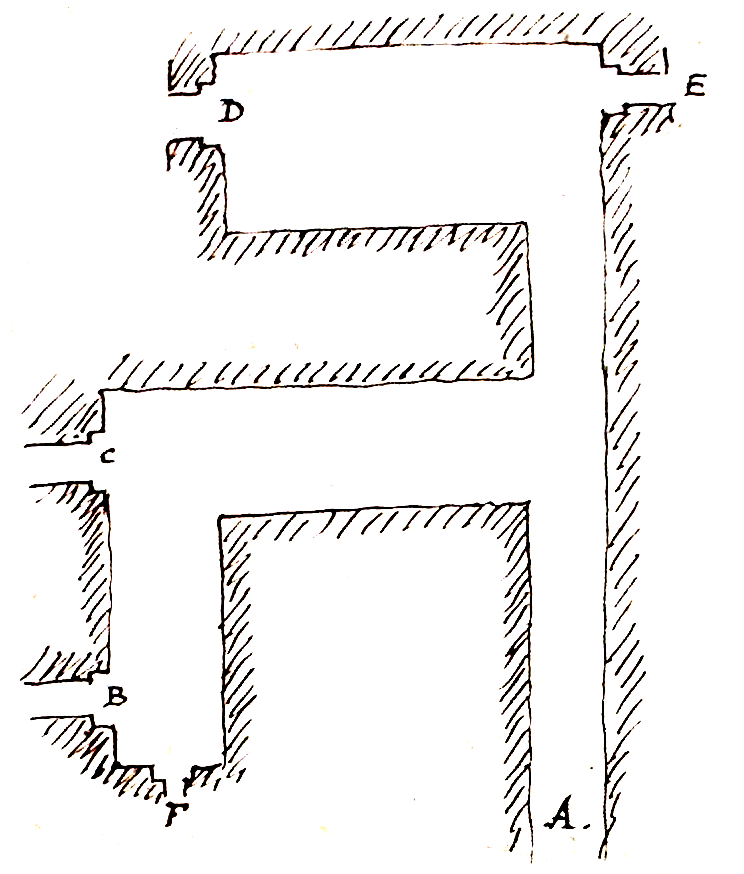
\includegraphics{CoEg_Mariette_1852-01-16_fig-1.png}
\end{center}
\indent Le plan incliné commence en A = B, C, D, E sont des portes qui\\
communiquent dans l’intérieur des souterrains à l’est par la porte B\\
que j’ai pénétrée le 12 novembre. F est une 5\textsuperscript{e} porte qui conduit\\
à des galeries inconnues, car elles sont ensablées jusqu’aux voutes [\textit{sic}].\\
{[rature]} Le plan incliné tout entier est, bien entendu, taillé dans\\
le roc. Or à hauteur d’appui sur chacune de ses parois, se\\
voient encore une quantité incroyable de stèles votives en\\
hiéroglyphes ou en démotiques. Le même fait se répète dans un\\
grand nombre de chambres de l’intérieur = Ce fait singulier\\
mérite, je crois, une grande attention et mon premier soin, à\\
la reprise des travaux, sera d’enlever toutes celles de ces stèles\\
que je pourrai rencontrer.\\
\indent J’ai encore bien des choses à vous dire. Mais, vous le voyez,\\
la place me manque. Ayez la complaisance de présenter mes hommages\\
à \hyperlink{CoEg_abbr_00000001}{M\textsuperscript{\underline{r}}} de Rougé\gls{CoEg_pers_00000032}, à \hyperlink{CoEg_abbr_00000001}{M\textsuperscript{\underline{r}}} de Longpérier\gls{CoEg_pers_00000033}, à \hyperlink{CoEg_abbr_00000001}{M\textsuperscript{\underline{r}}} de Viel-Castel\gls{CoEg_pers_00000034}\\
et à \hyperlink{CoEg_abbr_00000001}{M\textsuperscript{\underline{r}}} Villot\gls{CoEg_pers_00000035}. Si Dieu\gls{CoEg_pers_00000036} me conserve l’excellente santé dont je\\
jouis, je compte avoir encore ici du travail pour une année.\\
\indent Mais que de choses à faire.
\begin{center} \hspace{5cm} Votre tout dévoué serviteur :\\
\hspace{5cm} \hyperlink{CoEg_abbr_00000002}{Aug.} Mariette\end{center}

\hypertarget{CoEg_Mariette_1852-08-04}{}
\section*{Le 4 août 1852, d’Abousir, vraisemblablement à Nieuwerkerke, directeur général des musées nationaux}
\addcontentsline{toc}{section}{Le 4 août 1852, d’Abousir, vraisemblablement à Nieuwerkerke, directeur général des musées nationaux} 
{\footnotesize \noindent Institution et lieu de conservation~: Archives nationales, Pierrefitte-sur-Seine\\
Cote~: \hyperlink{CoEg_Mariette_ms_001}{20150497/118, dossier 145 «~Mariette, Auguste~»} (n. p.).\\
Support~: une feuille double.\\
Thèmes~: \gls{CoEg_keyword_00000011}, \gls{CoEg_keyword_00000006}~;\gls{CoEg_keyword_00000002} , \gls{CoEg_keyword_00000007}.\\
Note~: une copie non datée de cette lettre se trouve dans les papiers Mariette conservés au sein du fonds Maspero à la bibliothèque de l’Institut de France (ms.~4061 (2), f\textsuperscript{os}~24-27 pour cette lettre). Ces copies ne sont pas de la main de Mariette ni de Maspero, mais correspondent à une écriture ancienne (parmi elles, la lettre copiée la plus récente est de 1869). Elles mentionnent parfois que l’original se trouvait aux archives du Louvre. Cette copie n’est pas toujours très fiable, notamment pour les noms propres.
\begin{center} {[1\textsuperscript{re} page, r\textsuperscript{o}]}\end{center}}
\begin{flushright} Du désert d’Abousyr\gls{CoEg_place_00000008}, le 4 août 1852.\end{flushright}

\hspace{1cm}Monsieur\gls{CoEg_pers_00000002},\\

\indent J’ai écrit avant-hier à \hyperlink{CoEg_abbr_00000001}{M\textsuperscript{\underline{r}}} le Ministre de l’Intérieur\gls{CoEg_pers_00000037} pour l’avertir\\
du départ très-prochain d’Alexandrie\gls{CoEg_place_00000006} de trois de mes caisses. Ces\\
caisses seront vers le 15 août à Marseille\gls{CoEg_place_00000018}, et si le commissionnaire\footnote{La fin du mot est écrite par-dessus un autre mot illisible.}\\
de roulage de l’Intérieur\gls{CoEg_org_00000009} veut bien se hâter, vous les recevrez quelques\\
jours après.\\
\indent J’ai joint à ma lettre à \hyperlink{CoEg_abbr_00000001}{M\textsuperscript{\underline{r}}} le Ministre\gls{CoEg_pers_00000037} [rature] une autre\\
lettre pour \hyperlink{CoEg_abbr_00000009}{MM.} B{[oujon ?]}\gls{CoEg_pers_00000038} et Verrier\gls{CoEg_pers_00000039}, 75, rue de Rambuteau, aujourd’hui\\
chargés des transports de votre Ministère\gls{CoEg_org_00000009}. Ayez la bonté, Monsieur,\\
de faire dire à ces Messieurs l’intérêt que vous avez à posséder ces\\
caisses, et recommandez-leur surtout de ne les manier qu’avec\\
précautions, car les objets qu’ils contiennent, tout en pierre qu’ils\\
sont, sont des plus fragiles.\\
\indent Je prie aussi \hyperlink{CoEg_abbr_00000001}{M\textsuperscript{\underline{r}}} le Ministre de l’Intérieur\gls{CoEg_pers_00000037} de vous faire passer\\
une copie de l’extrait de mon catalogue que je lui ai envoyé. Cet\\
extrait concerne les monuments renfermés dans les trois colis. Je\\
vous serait très-obligé si vous vouliez bien réclamer cette copie\\
aux Beaux-Arts\gls{CoEg_org_00000011}.\\
\indent J’aurais voulu joindre à cet envoi quelque monument qui, pour\\
son exécution artistique, vous intéressât plus particulièrement. Mais\\
les caisses sont trop lourdes, ou bien elles sont encore ici et vont\\
faire partie d’une seconde expédition pour Alexandrie\gls{CoEg_place_00000006}. Je tâcherai\\
néanmoins de vous faire passer un de ces jours mon \textit{écrivain\gls{CoEg_obj_00000008}}. Ce\\
monument est au moins de la IV\textsuperscript{e} dynastie et il surpasse, pour le\\
modelé des chairs et l’expression générale du personnage, tout ce\\
que vous avez vu jusqu’ici, même de ce qu’on appelle la bonne époque.\\
La photographie que je vous en ai envoyée a mal rendu ces formes si\\
naturelles, et vous ne devez pas la regarder comme une copie exacte du modèle.
{\footnotesize \begin{center} {[1\textsuperscript{re} page, v\textsuperscript{o}]}\end{center}}
\indent J’ai jusqu’ici livré au gouvernement égyptien\gls{CoEg_org_00000008} 656 monuments, et je\\
m’arrange de manière à passer pour n’en garder aucun par devers moi,\\
ce qui, entre nous, est tout de la contraire de la vérité. Son Altesse\gls{CoEg_pers_00000016} sera\\
enchantée quand elle apprendra mon empressement à obéir à ses\\
ordres et elle n’en sera que plus disposée à nous faire plus tard\\
un second cadeau. Mais pour cela je pense qu’il faudrait, dès-\\
-à-présent, que le nouveau consul-général\gls{CoEg_pers_00000040} d’Egypte\gls{CoEg_place_00000003} (de qui tout\\
dépend) fût instruit par le Ministre des Affaires Etrangères\gls{CoEg_pers_00000041} de l’importance\\
que le gouvernement français\gls{CoEg_org_00000012} attache aux fouilles du Sérapéum\gls{CoEg_place_00000004}, afin\\
qu’il ne soit plus, comme \hyperlink{CoEg_abbr_00000001}{M\textsuperscript{\underline{r}}} Le Moyne\gls{CoEg_pers_00000024}, qu’on a laissé un an\\
sans instruction, exposé à pêcher {[\textit{sic}]} par ignorance. Causez-en avec\\
\hyperlink{CoEg_abbr_00000001}{M\textsuperscript{\underline{r}}} Batissier\gls{CoEg_pers_00000027}, et celui-ci vous dira que si le nouveau Consul-\\
-général\gls{CoEg_pers_00000040} le veut bien, il peut obtenir de Son Altesse\gls{CoEg_pers_00000016} même le droit\\
de fouiller dans l’Egypte\gls{CoEg_place_00000003} entière, ce que je désire bien vivement,\\
Monsieur, car il m’en coûterait beaucoup de retourner en France\\
sans avoir visité Thèbes\gls{CoEg_place_00000019} et la Haute-Egypte\gls{CoEg_place_00000020}.\\
\indent \hyperlink{CoEg_abbr_00000001}{M\textsuperscript{\underline{r}}} D’Anastasy\gls{CoEg_pers_00000015} est mort il y a quelques jours\footnote{Il s'agissait d'une fausse rumeur (voir la \hyperref{CoEg_Mariette_1852-09-04}{lettre du 4 septembre 1852})~; Anastasi\gls{CoEg_pers_00000015} mourrut en 1860.} et peut-être\\
ses héritiers n’auront-ils pas la même prétention quant à la\\
collection de Livourne\gls{CoEg_place_00000012}. J’ai déjà écrit à Alexandrie\gls{CoEg_place_00000006} pour qu’on\\
sonde le terrain à ce sujet et je vous ferai part de toutes les\\
informations que je pourrai recueillir. De votre côté, dites-moi\\
si, avec une réduction considérable de prix, vous seriez disposé à\\
terminer cette affaire.\\
\indent Rien de nouveau ici. J’attends avec impatience le moment de\\
reprendre les travaux et les souterrains grecs m’empêchent de\\
dormir. Du reste, si on m’accorde des fonds, je pousserai les fouilles\\
avec la plus grande activité, car j’ai hâte d’en finir. En six mois\\
j’espère que tout sera fait.
{\footnotesize \begin{center} {[2\textsuperscript{e} page, r\textsuperscript{o}]}\end{center}}
\indent Mais le plus difficile sera d’emballer les grands lions\gls{CoEg_obj_imn} grecs\\
et les autres statues de même style. Ces objets ont été taillés dans\\
une pierre très-friable qui s’écaille et je ne vois pas de moyen de\\
les ramener sans les briser. Aussi, Monsieur, je m’adresse à vous\\
et je vous prie de me faire savoir si vous ne connaissez pas\\
quelque composition chimique qui rende à la pierre sa dureté\\
primitive.\footnote{En juillet 1851, Rochas publia dans les comptes rendus de l'Académie des sciences une lettre sur le procédé de silicatisation~; il mentionnait un voyage en Orient au cours duquel il avait observé les monuments du Sérapéum et échangé avec Mariette à ce sujet (\textsc{Rochas}, «~Moyens de conserver indéfiniment les monuments en pierre calcaire~»\gls{CoEg_bibl_00000005}, \textit{Comptes-rendus de l’Académie des sciences}, 1851, p. 622~:\\
«~Qu’il me soit permis, en terminant cette Lettre, d’appeler l’attention de l’Académie sur les monuments découverts récemment par M. Mariette, dans les fouilles qu’il exécute dans le temple de Sérapis, à Memphis. Au commencement de cette année, lors de mon voyage en Orient, j’eus occasion de visiter sur les lieux les statues, les sphinx, \hyperlink{CoEg_abbr_00000052}{etc.}, qui étaient à découvert à cette époque. Ces monuments sont la plupart en calcaire tendre de la chaîne arabique, qui offre naturellement peu de cohésion. Je reconnus, qu’étant resté enfoui pendant tant de siècles, ce calcaire était, pour ainsi dire, totalement privé de solidité~; en effet, peu de temps après que ces statues eurent été exposées à l’air, après leur exhumation, elles se sont écaillées et détériorées si promptement, que l’on a jugé indispensable de les faire recouvrir de sable.\\
\indent M. Mariette me fit part des inquiétudes qu’il éprouvait pour la conservation et le transport en France de ces statues~; je lui fis remarquer alors qu’il était possible de leur donner sur place, en les silicatisant, la solidité nécessaire pour le transport, et je lui offris de me charger de cette opération.~»\\
Le département égyptien du Louvre constitua d'ailleurs en 1853 un dossier à ce sujet - conservé sous la cote 20144775/24 aux Archives nationales. Rochas obtint l'autorisation de faire des essais de son procédé sur des statues égyptiennes du Louvre (voir aussi l'article 20144793/33 des Archives nationales où se trouvent des courriers archivés par le département des sculptures).} Dans ce cas, veuillez me la faire connaître, afin que\\
je l’applique ici, car les monuments dont je vous entretiens, sans\\
être très-précieux au point de vue de l’art, le sont beaucoup\\
pour les archéologues, et dans tous les cas feront toujours au\\
Louvre\gls{CoEg_org_00000002} un excellent fond de salle. En attendant que vous veuillez\\
bien me répondre, ces monuments sont sous le sable à l’abri de\\
toute cause de destruction.\\
\indent Je ne compte pas vous envoyer toutes les statues\gls{CoEg_obj_imn} grecques de\\
l’hémicycle de l’Apéum. Elles sont trop mauvaises. J’en ferai\\
un choix d’une ou deux. Mais je vous demanderai à mouler\\
les autres à cause des inscriptions grecques qu’on y lit.\\
\indent Vous aurez remarqué sans doute dans mon plan général\\
de la tombe d’Apis\gls{CoEg_pers_00000011} et d’Osiris\gls{CoEg_pers_00000151} l’indication, dans la tombe\\
d’Osiris\gls{CoEg_pers_00000151}, de quelques salles éboulées. J’ai oublié de noter, dans\\
mon programme des travaux qui restent à faire, le déblaiement\\
de ces salles. Je les ai bien nettoyées jusqu’à un mètre du sol,\\
mais pas assez pour être sûr qu’ils n’y reste rien. Il existe là\\
en effet d’énorme rochers qui recouvrent peut-être des monuments\\
précieux et que j’ai craint de faire sauter. Je crois bien que\footnote{Mariette\gls{CoEg_pers_00000001} avait écrit «~qu'~», mais a biffé l'apostrophe et complété en «~que~».} des\\
fouilles plus attentives dans cette partie du Sérapéum\gls{CoEg_place_00000004} pourront\\
ne pas être improductives.
{\footnotesize \begin{center} {[2\textsuperscript{e} page, v\textsuperscript{o}]}\end{center}}
\indent J’ai à vous remercier beaucoup, Monsieur, à vous remercier du\\
fond de mon cœur de ce que vous avez bien voulu [pour ma femme\gls{CoEg_pers_00000005} ?]\footnote{Si «~ma~» est assez clair, le premier mot pourrait se lire «~fait~».}.\\
Vous savez bien que mon dévouement et celui de toute ma famille\\
vous est acquis et je n’ai pas besoin de vous exprimer par de\\
plus longues phrases un sentiment que vous savez sincère. Je suis\\
tout entier à vos ordres et prêt pour vous à aller, si vous le voulez,\\
au bout du monde.\\
\indent Hier j’ai fait cuire des œufs sous le sable. Le soleil nous dévore\\
et le sable est si chaud qu’on ne peut littéralement en tenir une\\
poignée dans la main. Heureusement nous touchons au terme\\
de ces chaleurs accablantes. Le Nil\gls{CoEg_place_00000021} monte et couvre déjà les\\
campagnes~; la fraîcheur vient avec lui. Quel beau pays que\\
l’Egypte\gls{CoEg_place_00000003} et comme le temps des\footnote{Le mot a été inscrit sur d'autres lettres.} Ramsès reviendrait pour lui\\
s’il était à la France\gls{CoEg_org_00000012}. En attendant les Anglais le convoitent\\
bien et ne tarderont pas à en faire leur Algérie\gls{CoEg_place_00000022}. Adieu alors\\
les antiquités pour le Louvre\gls{CoEg_org_00000002}, adieu le Sérapéum\gls{CoEg_place_00000004} que le sable\\
recouvre encore.\\
\indent Présentez, s’il vous plaît, mes civilités à \hyperlink{CoEg_abbr_00000001}{M\textsuperscript{\underline{r}}} de Viel-Castel\gls{CoEg_pers_00000034},\\
à \hyperlink{CoEg_abbr_00000001}{M\textsuperscript{\underline{r}}} de Longpérier\gls{CoEg_pers_00000033}, à \hyperlink{CoEg_abbr_00000001}{M\textsuperscript{\underline{r}}} Villot\gls{CoEg_pers_00000035}, à \hyperlink{CoEg_abbr_00000001}{M\textsuperscript{\underline{r}}} Auguiot\gls{CoEg_pers_00000044}, à \hyperlink{CoEg_abbr_00000001}{M\textsuperscript{\underline{r}}} Sauzay\gls{CoEg_pers_00000043},\\
et à bien d’autres que j’oublie sans doute, car depuis bientôt\\
deux ans j’ai eu le temps de laisser ma pauvre mémoire s’envoler\\
avec le vent du désert. Quant à vous, Monsieur, je n’ai pas\\
besoin de vous renouveler l’assurance de tous mes sentiments\\
de respect. Vous savez que je suis tout à vous
\begin{center} \hspace{5cm}\hyperlink{CoEg_abbr_00000002}{Aug.} Mariette\end{center}
Je vous fais mes excuses pour une bien mauvaise petite boîte qui s’est\\
glissée dans le colis qui vous a été apportée par Batissier\gls{CoEg_pers_00000027}. Cette petite\\
boîte ne contenait que du rebut, et elle a été envoyée par erreur au\\
Caire\gls{CoEg_place_00000010}.\\
\indent Faites-moi le plaisir de bien remercier pour moi Batissier\gls{CoEg_pers_00000027} de tous\\
les services qu’il m’a rendu au Caire\gls{CoEg_place_00000010}. Dieu\gls{CoEg_pers_00000036} veuille que je revoie bientôt cet excellent
\begin{flushright}ami.\end{flushright}

\hypertarget{CoEg_Mariette_1852-08-20}{}
\section*{Le 20 août 1852, d’Abousir, à Persigny, ministre de l'Intérieur}
\addcontentsline{toc}{section}{Le 20 août 1852, d’Abousir, à Persigny, ministre de l'Intérieur} 
{\footnotesize \noindent Institution et lieu de conservation~: Archives nationales, Pierrefitte-sur-Seine\\
Cote~: \hyperlink{CoEg_Mariette_ms_001}{20150497/118, dossier 145 «~Mariette, Auguste~»} (n. p.).\\
Support~: une feuille double.\\
Thèmes~: \gls{CoEg_keyword_00000002}, \gls{CoEg_keyword_00000007}.\\
Note~: une copie non datée de cette lettre se trouve dans les papiers Mariette conservés au sein du fonds Maspero à la bibliothèque de l’Institut de France (ms.~4061 (2), f\textsuperscript{os}~28-29 pour cette lettre). Ces copies ne sont pas de la main de Mariette ni de Maspero, mais correspondent à une écriture ancienne (parmi elles, la lettre copiée la plus récente est de 1869). Elles mentionnent parfois que l’original se trouvait aux archives du Louvre. Cette copie n’est pas toujours très fiable, notamment pour les noms propres.
\begin{center} [1\textsuperscript{re} page, r\textsuperscript{o}]
\end{center}}
\begin{flushright}
Du désert d’Abousyr\gls{CoEg_place_00000008}, le 20 août 1852.
\end{flushright}
\indent A Monsieur\\
\begin{center}Monsieur le Ministre Secrétaire d’État au département\end{center}
\begin{flushright}de l’Intérieur\gls{CoEg_org_00000009}, à Paris\gls{CoEg_place_00000002}.\end{flushright}

\hspace{1cm} Monsieur le Ministre\gls{CoEg_pers_00000037},\\

\indent Par ma lettre en date du 1\textsuperscript{er} Août dernier, j’ai eu l’honneur\\
de vous faire savoir que je venais de m’entendre avec \hyperlink{CoEg_abbr_00000001}{M\textsuperscript{\underline{r}}} le Consul-\\
Général\gls{CoEg_pers_00000024} de France\gls{CoEg_org_00000012} à Alexandrie\gls{CoEg_place_00000006} à l’effet d’expédier, à destination\\
de Marseille\gls{CoEg_place_00000018}, trois colis d’antiquités provenant du Sérapéum\gls{CoEg_place_00000004}\\
de Memphis\gls{CoEg_place_00000005}. – J’avais alors entre les mains une lettre de \hyperlink{CoEg_abbr_00000001}{M\textsuperscript{\underline{r}}} le\\
second \gls{CoEg_entry_00000006}\gls{CoEg_pers_imn} du Consulat-Général\gls{CoEg_org_00000006} qui m’autorisait à vous\\
faire cette déclaration, et d’un autre côté je savais officieusement\\
notre honorable consul-général\gls{CoEg_pers_00000024} tout disposé à seconder mes intentions\\
à l’égard du transport de ces mêmes colis.\\
\indent Mais à l’époque où nous décidions ensemble cette mesure,\\
le vapeur qui devait être chargé du transport n’était pas encore\\
à Alexandrie\gls{CoEg_place_00000006} et nous ne devions pas supposer qu’un empêchement\\
quelconque pût se présenter. C’est pourtant ce qui advint et il\\
résulte de la copie de la lettre de \hyperlink{CoEg_abbr_00000001}{M\textsuperscript{\underline{r}}} Le Moyne\gls{CoEg_pers_00000024} jointe ici\footnote{La lettre en question est recopiée par Mariette\gls{CoEg_pers_00000001} à la main sur la deuxième page de la feuille, en-tête compris.} qu’à\\
son arrivée à Alexandrie\gls{CoEg_place_00000006} le capitaine du bâtiment, consulté\\
à ce sujet, déclara ne pouvoir se charger de l’embarquement
\begin{flushright}de trois\end{flushright}
{\footnotesize \begin{center} {[1\textsuperscript{re} page, v\textsuperscript{o}]}\end{center}}
de trois caisses. J’ai donc à vous prier aujourd’hui de regarder comme\\
non avenue ma lettre du 1\textsuperscript{er} Août~; les antiquités que j’eusse\\
désiré expédier en France\gls{CoEg_place_00000016} le plus promptement possible attendront\\
avec les autres dans les magasins du Consulat-Général\gls{CoEg_org_00000006} le\\
navire de guerre que je vous supplie de nouveau de vouloir\\
bien nous faire envoyer.\\
\indent D’ailleurs, Monsieur le Ministre, vous voudrez bien\\
considérer que la fausse démarche que j’ai faite le 1\textsuperscript{er} août\\
était inévitable, tant par la nécessité où je me trouvais de\\
vous informer de la résolution prise, que par la distance qui\\
me sépare d’Alexandrie\gls{CoEg_place_00000006} et l’arrivée tardive du bateau-poste\\
dans le port de cette ville. La lettre de \hyperlink{CoEg_abbr_00000001}{M\textsuperscript{\underline{r}}} le Consul-Général\gls{CoEg_pers_00000024}\\
porte en effet la date du 4 août~; elle m’est ainsi arrivée\\
le 7, c’est-à-dire le jour même du départ du paquebot qui\\
emportait ma lettre d’avis. Je ne crois donc pas qu’il y ait\\
de ma faute si la nouvelle que je me suis hâté de porter à\\
votre connaissance a pu exposer vos bureaux à des démarches\\
inutiles.\\
\indent J’ai l’honneur d’être avec le plus profond respect,
\begin{center} Monsieur le Ministre,\end{center}
\begin{center}\hspace{5cm} Votre très-humble\\
\hspace{5cm} et très-obéissant serviteur.\\
\hspace{5cm} \hyperlink{CoEg_abbr_00000002}{Aug.} Mariette\end{center}
{\footnotesize \begin{center} {[2\textsuperscript{e} page, r\textsuperscript{o}]}\end{center}}
Copie.\\
Agence et Consulat Général\gls{CoEg_org_00000006}\\
\hspace{3cm} de France\gls{CoEg_org_00000012}\\
\hspace{3cm} en Egypte\gls{CoEg_place_00000003}.
\begin{flushright}Alexandrie\gls{CoEg_place_00000006}, le 4 avril 1852.\end{flushright}
\begin{flushright}Monsieur \hyperlink{CoEg_abbr_00000002}{Aug.} Mariette\gls{CoEg_pers_00000001}, à Abousyr\gls{CoEg_place_00000008}.\end{flushright}

\hspace{1cm} Monsieur,\\

\indent D’après la lettre que vous m’avez fait l’honneur de m’écrire le 29\\
du mois dernier, j’ai prié \hyperlink{CoEg_abbr_00000001}{M\textsuperscript{\underline{r}}} le Commandant du paquebot français qui\\
se trouve actuellement dans le port d’Alexandrie\gls{CoEg_place_00000006} de venir voir les trois\\
caisses que vous désirez faire parvenir aussi promptement que possible\\
en France\gls{CoEg_place_00000016}~; mais ce commandant, après les avoir examinées, m’a\\
dit qu’il n’avait pas à son bord d’appareil assez fort pour soulever\\
et embarquer notamment la caisse \hyperlink{CoEg_abbr_00000010}{n\textsuperscript{o}} 40, en un mot, qu’il ne\\
pouvait pas se charger de la prendre à cause de son poids et de\\
sa grandeur~; dans cet état de choses, j’ai pensé qu’il y avait d’autant\\
moins d’inconvénients à suspendre l’envoi des deux autres caisses\\
\hyperlink{CoEg_abbr_00000011}{n\textsuperscript{os}} 4 et 7 que, sans doute, un bâtiment de l’État\gls{CoEg_org_00000012} ne devra plus\\
beaucoup tarder maintenant à venir chercher tous vos monuments.\\
Du reste lorsqu’il s’agira de leur départ, je me chargerai volontiers\\
de les adresser à \hyperlink{CoEg_abbr_00000001}{M\textsuperscript{\underline{r}}} l’Agent du Ministère des Affaires Etrangères\gls{CoEg_org_00000007}\\
à Marseille\gls{CoEg_place_00000018} pour les consigner à \hyperlink{CoEg_abbr_00000001}{M\textsuperscript{\underline{r}}} \hyperlink{CoEg_abbr_00000012}{Eug.} Pastré\gls{CoEg_pers_00000046} ....\\
\indent Agréez, Monsieur – \hyperlink{CoEg_abbr_00000052}{etc.}
\begin{center} \hspace{5cm} Signé A. Le Moyne \gls{CoEg_pers_00000024}.\end{center}

\hypertarget{CoEg_Mariette_1852-09-03}{}
\section*{Le 3 septembre 1852, d’Abousir, à Persigny, ministre de l'Intérieur}
\addcontentsline{toc}{section}{Le 3 septembre 1852, d’Abousir, à Persigny, ministre de l'Intérieur}
{\footnotesize \noindent Institution et lieu de conservation~: Archives nationales, Pierrefitte-sur-Seine\\
Cote~: \hyperlink{CoEg_Mariette_ms_001}{20150497/118, dossier 145 «~Mariette, Auguste~»} (n. p.).\\
Support~: une feuille double.\\
Thèmes~: \gls{CoEg_keyword_00000012}, \gls{CoEg_keyword_00000002}.\\
Note~: \begin{itemize} \item La lettre porte, d’une autre main que celle de Mariette, au crayon rouge et au coin supérieur gauche~: «~lettres de \hyperlink{CoEg_abbr_00000001}{M\textsuperscript{\underline{r}}}/Mariette~»~; et au crayon gris~: «~A classer~»~;
\item Une copie non datée de cette lettre se trouve dans les papiers Mariette conservés au sein du fonds Maspero à la bibliothèque de l’Institut de France (ms.~4061 (2), f\textsuperscript{os}~30-33 pour cette lettre). Ces copies ne sont pas de la main de Mariette ni de Maspero, mais correspondent à une écriture ancienne (parmi elles, la lettre copiée la plus récente est de 1869). Elles mentionnent parfois que l’original se trouvait aux archives du Louvre. Cette copie n’est pas toujours très fiable, notamment pour les noms propres. \end{itemize}
\begin{center} {[1\textsuperscript{re} page, r\textsuperscript{o}]}\end{center}}

\begin{flushright} Du désert d’Abousyr\gls{CoEg_place_00000008}, le 3 septembre 1852.\end{flushright}
\indent A Monsieur\\
\begin{center}Monsieur le Ministre Secrétaire d’Etat au Département\\
de l’Intérieur\gls{CoEg_org_00000009}\end{center}
\begin{flushright}à Paris\gls{CoEg_place_00000002}.\end{flushright}

\hspace{1cm}Monsieur le Ministre\gls{CoEg_pers_00000037},\\

\indent J’ai déjà eu souvent l’occasion de vous entretenir de la position\\
difficile qui résulte pour moi des conventions arrêtées au mois de février\\
dernier entre le \gls{CoEg_entry_00000002}\gls{CoEg_pers_00000016} d’Egypte\gls{CoEg_place_00000003} et le gouvernement français\gls{CoEg_org_00000012}. En vertu de\\
ces conventions, mon droit de fouiller ne s’étend pas au-delà du Sérapéum\gls{CoEg_place_00000004}\\
de Memphis\gls{CoEg_place_00000005} et chacun des objets découverts appartient de droit au gouvernement\\
égyptien\gls{CoEg_org_00000008} qui s'en empare aussitôt trouvés et les fait transporter à la Citadelle\gls{CoEg_place_00000023}\\
du Caire\gls{CoEg_place_00000010}. Deux officiers d’état-major de l’armée égyptienne\gls{CoEg_org_00000013} stationnent\\
continuellement sur les lieux, enregistrent jour par jour les résultats obtenus\\
et veillent à ce que rien ne soit détourné. C’est ainsi que, depuis le\\
mois de février jusqu’au mois de juin, j’ai été forcé de livrer à ces agents\\
656 objets antiques.\\
\indent Je viens de vous dire que ces conventions me faisaient une position\\
très-difficile. En effet, d’une part, je ne crois pas devoir vous cacher mon\\
désir d’aller visiter, après l’achèvement des travaux du Sérapéum\gls{CoEg_place_00000004}, les ruines\\
de la Haute-Egypte\gls{CoEg_place_00000020} que je n’ai jamais vues et que, pour moi qui fais\\
profession d’égyptologie, il serait trop dur de ne jamais voir après les avoir\\
approchées de si près~; or un voyage de cette sorte, entrepris en érudit plutôt\\
qu’en touriste, exige toujours quelques petites déblaiements, puisque la plupart\\
des inscriptions de l’Egypte\gls{CoEg_place_00000003} ne peuvent être copiées et étudiées qu’à condition\\
d’écarter le sable qui les couvre, ce qui, depuis près d’une année, est formellement\\
interdit à tous les voyageurs. D’autre part je suis obligé de vous rappeler\\
que les circonstances me forcent à violer ces mêmes conventions arrêtées entre\\
\begin{flushright}les deux\end{flushright}
 {\footnotesize \begin{center} {[1\textsuperscript{re} page, v\textsuperscript{o}]}\end{center}}
les deux gouvernements et que loin de livrer au \gls{CoEg_entry_00000002}\gls{CoEg_pers_00000016} les monuments découverts\\
je lui laisse ceux de ces objets qui me semblent n’avoir aucune valeur, et que\\
j’organise pour les autre un système de contrebande qu’à cause même de sa\\
hardiesse je crains toujours de voir s’écrouler. C’est là, Monsieur le Ministre,\\
ce qui me fait la situation dont je me plains, situation sur laquelle\\
j’appelle toute votre attention, parce qu’elle est très-délicate et en même\\
temps très-périlleuse.\\
\indent Je viens donc vous prier de vouloir bien, dans le cas où vous\\
adopteriez ces vues, vous entendre avec \hyperlink{CoEg_abbr_00000001}{M\textsuperscript{\underline{r}}} le Ministre des Affaires Etrangères\gls{CoEg_pers_00000041} et\\
faire donner au nouveau Consul-Général\gls{CoEg_pers_00000040} de France\gls{CoEg_org_00000012} en Egypte\gls{CoEg_place_00000003} des instructions\\
au nom desquelles cet agent pourrait travailler à faire obtenir, en ce qui\\
me concerne, des conditions un peu plus libérales. Je crois devoir vous faire\\
observer à ce sujet que ce que j’ai l’honneur de vous proposer me paraît d’autant\\
moins dangereux à solliciter du Vice-Roi\gls{CoEg_pers_00000016} que le gouvernement français\gls{CoEg_org_00000012}, en\\
m’envoyant l’ordre exprès de livrer les objets découverts, a reconnu par là\\
même le droit de \hyperlink{CoEg_abbr_00000003}{S. A.}\gls{CoEg_pers_00000016} et a donné en même temps la preuve de son désir\\
d’entretenir avec elle des relations amicales. Les 656 objets que j’ai livrés me\\
paraissent ainsi un argument en notre faveur. – D’un autre côté, peut-être\\
les conditions dans lesquelles nous nous trouvons aujourd’hui ne sont-elles\\
plus les mêmes qu’au mois de février dernier. Mes travaux, vous vous le\\
rappelez, étaient suspendus depuis le 21 novembre, et le 12 septembre auparavant\\
l’ordre m’avait été donné, de la part du Vice-Roi\gls{CoEg_pers_00000016}, de livrer tous les\\
monuments que j’avais en magasin. Mais le Vice-Roi\gls{CoEg_pers_00000016} n’était, en quelque\\
sorte, pour rien dans cette affaire~; il était poussé aux mesures un peu\\
violentes dont je fus alors l’objet par son conseiller ordinaire, \hyperlink{CoEg_abbr_00000001}{M\textsuperscript{\underline{r}}} le\\
Consul-Général anglais\gls{CoEg_pers_00000018}. Ce n’est pas en effet que le \gls{CoEg_entry_00000002}\gls{CoEg_pers_00000016} attache un\\
grand prix aux antiquités qui couvrent son royaume et qu’il ait regardé\\
mes découvertes comme une spoliation de son propre bien : vous savez au\\
contraire avec quelle désolante persévérance ses agents détruisent un à un\\
les vénérables témoins de la grandeur des Pharaons. Ce n’est pas non plus\\
qu’il eût eu sérieusement l’idée, ou de s’approprier mes monuments, ou de\\
m’empêcher de continuer mes travaux~; je crois que si nous avions résolument\\
cédé devant des exigences, en réservant notre recours à l’opinion publique,\\
{\footnotesize \begin{center} {[2\textsuperscript{e} page, r\textsuperscript{o}]}\end{center}}
\noindent nous eussions été moins embarrassés de notre défaite que \hyperlink{CoEg_abbr_00000001}{M\textsuperscript{\underline{r}}} Murray\gls{CoEg_pers_00000018} et lui\\
d’une victoire qu’ils ne cherchaient pas, qu’ils ne désiraient pas, parce que\\
{\small le droit seul \textsuperscript{qu’ils invoquaient} ne suffisait pas pour prendre violemment possession des monuments}\\
acquis avec l’argent de la France\gls{CoEg_org_00000012} et l’autorisation régulière du \gls{CoEg_entry_00000002}\gls{CoEg_pers_00000016}\\
lui-même. Ce qu’on voulait au contraire, c’était que par nos fautes nous\\
créassions \sout{[un~?] droit} nous-mêmes un droit nouveau à \hyperlink{CoEg_abbr_00000003}{S. A.}\gls{CoEg_pers_00000016}, et pour cela\\
on a affecté de traiter directement avec moi sans passer par l’intermédiaire\\
obligé du Consul-Général\gls{CoEg_pers_00000024}, afin de profiter de mon inexpérience et de faire\\
naître par ma propre incapacité une raison légitime de garder les monuments\\
confisqués et de m’interdire l’accès du Sérapéum\gls{CoEg_place_00000004}. Deux mois après, les\\
Anglais se fussent installés sur les ruines que, selon eux, nous n’eussions\\
pas su garder et les 515 monuments confisqués eussent bientôt après pris\\
incognito le chemin de Londres\gls{CoEg_place_00000011} avec ceux que la continuation des fouilles\\
eût fait découvrir. Je vous répète donc, Monsieur le Ministre, que tout cela\\
a été le résultat d’une intrigue anglaise~; mais j’ajoute que peut-être\\
aujourd’hui les réclamations de notre consul-général\gls{CoEg_pers_00000040} ne trouveraient pas\\
\hyperlink{CoEg_abbr_00000003}{S. A.}\gls{CoEg_pers_00000016} dans les mêmes dispositions.\\
\indent En tout cas, \hyperlink{CoEg_abbr_00000001}{M\textsuperscript{\underline{r}}} Sabatier\gls{CoEg_pers_00000040} pourra sans doute à son arrivée\\
sonder le terrain et je pense, Monsieur le Ministre, que si le moment venait\\
où ce fonctionnaire croirait pouvoir risquer la demande que j’ai l’honneur\\
de vous soumettre, il devrait d’autant mieux saisir l’occasion que le\\
changement tout récent de \Gls{CoEg_entry_00000004} de la province de Gyzeh\gls{CoEg_place_00000007} va amener\\
un mouvement dans le personnel de mes officier et que je ne sais pas s’il\\
me sera toujours possible d’échapper à la surveillance de ces gens et de\\
sauver au profit du Louvre\gls{CoEg_org_00000002} les monuments nouveaux que la reprise des\\
travaux pourra me faire découvrir.\\
\indent J’ai l’honneur d’être avec le plus profond respect,
\begin{center}Monsieur le Ministre,\end{center}
\begin{center}\hspace{5cm}Votre très-humble\\
\hspace{5cm}et très-obéissant serviteur.\\
\hspace{5cm}\hyperlink{CoEg_abbr_00000002}{Aug.} Mariette\end{center}
{\footnotesize\begin{center} {[2\textsuperscript{e} page, v\textsuperscript{o}]}\end{center}
\noindent \hyperlink{CoEg_abbr_00000008}{P. S.} Après avoir rappelé au commencement de cette lettre les conditions qui nous sont imposées par le\\
gouvernement\gls{CoEg_org_00000008} du \gls{CoEg_entry_00000002}\gls{CoEg_pers_00000016}, je crois devoir vous faire connaître celles que, dans les mêmes circonstances,\\
le Vice-Roi\gls{CoEg_pers_00000016} a consenties en faveur du gouvernement anglais\gls{CoEg_org_00000014}. Il y a un an environ, la Société Géologique\gls{CoEg_org_00000015}\\
de Londres\gls{CoEg_place_00000011} manifesta le désir de faire quelques excavations sur le sol des anciennes capitales de\\
l’Egypte\gls{CoEg_place_00000003}. L’enceinte d’Héliopolis\gls{CoEg_place_00000024} fut explorée l’été passé, et la saison actuelle a été occupée par\\
de grandes fouilles sur l’emplacement de Memphis\gls{CoEg_place_00000005}. Mais, ainsi que j’ai pu m’en assurer par\\
des visites presque quotidiennes, la géologie n’est, à Memphis\gls{CoEg_place_00000005} du moins, que l’accessoire de\\
l’archéologie, et c’est le Musée Britannique\gls{CoEg_org_00000005} qui, surtout, profitera de ces travaux. En effet de\\
longues tranchées ont été ouvertes autour du colosse de Ramsès II\gls{CoEg_pers_00000026} à Myt-Rahyneh\gls{CoEg_place_00000025} et poussées\\
dans toutes les directions à travers les buttes de décombres qui recouvrent Memphis\gls{CoEg_place_00000005}. Chacune\\
de ces buttes a été ouverte, et en ce moment même les travailleurs de la Société\gls{CoEg_org_00000015}, chassés des\\
terres cultivées par l’inondation, viennent s’installer au milieu des sables de la nécropole\\
avec lesquels la géologie ne peut avoir rien à faire. Ces recherches, poursuivies avec\\
persévérance depuis cinq mois, n’ont pas été vaines~; l’emplacement et les limites du temple\\
de Ptah\gls{CoEg_pers_00000047} sont reconnus, les restes d’un nombre incroyable de colosses en granit sont retrouvés,\\
et le British Muséum\gls{CoEg_org_00000005} va s’enrichir d’une cinquantaine de statuettes de toute matière,\\
débris de l’ancienne splendeur du fameux temple de Vulcain\gls{CoEg_pers_00000047}. – Or ces recherches\\
se font toutes exclusivement aux frais du gouvernement égyptien\gls{CoEg_org_00000008}. Aussitôt que l’intention\\
de la Société Géologique\gls{CoEg_org_00000015} a été connue, \hyperlink{CoEg_abbr_00000003}{S. A.}\gls{CoEg_pers_00000016} s’est empressée de mettre à la disposition de\\
\hyperlink{CoEg_abbr_00000001}{M\textsuperscript{\underline{r}}} Murray\gls{CoEg_pers_00000018}, outre \hyperlink{CoEg_abbr_00000004}{S. E.} Hékékyan-\gls{CoEg_entry_00000003}\gls{CoEg_pers_00000048} comme directeur, un capitaine d’état-major comme\\
surveillant-général, trois ingénieurs détachés pour ce service du \gls{CoEg_entry_00000007} des Travaux Publics\gls{CoEg_org_00000016},\\
et des ouvriers en aussi grand nombre qu’il pourrait en désirer. Le traitement de ces\\
agents et des hommes à leurs ordres constitue, avec les frais d’approvisionnement, de\\
campement, de machines, d’outils \hyperlink{CoEg_abbr_00000052}{etc.} – une dépense de près de 6 000 \hyperlink{CoEg_abbr_00000013}{fr.} par mois que le\\
\gls{CoEg_entry_00000002}\gls{CoEg_pers_00000016} supporte en faveur de l’Angleterre\gls{CoEg_org_00000014}. Ajoutez que, loin de contester à \hyperlink{CoEg_abbr_00000001}{M\textsuperscript{\underline{r}}} Murray\gls{CoEg_pers_00000018}\\
le droit de posséder les antiquités provenant de ces fouilles, \hyperlink{CoEg_abbr_00000003}{S. A.}\gls{CoEg_pers_00000016} fait les frais de leur transport\\
jusqu’à Alexandrie\gls{CoEg_place_00000006}. Enfin Hékékyan-\gls{CoEg_entry_00000003}\gls{CoEg_pers_00000048} devant incessamment porter ses recherches sur\\
Abydos\gls{CoEg_place_00000026} et Thèbes\gls{CoEg_place_00000019}, le gouvernement égyptien\gls{CoEg_org_00000008} met à sa disposition un bâteau {[\textit{sic}]} à vapeur.\\
– Tels sont, Monsieur le Ministre, les avantages faits en cette circonstance à l’Angleterre\gls{CoEg_org_00000014}.\\
Je n’établis pas ce parallèle parce que je désire jouir des mêmes facilités que Hékékyan-\\
-\gls{CoEg_entry_00000003}\gls{CoEg_pers_00000048}, et je ne crois pas non plus que la France\gls{CoEg_org_00000012} se soucie beaucoup de la collaboration\\
d’Abbas-\Gls{CoEg_entry_00000002}\gls{CoEg_pers_00000016}. Ce que je demande, c’est que le gouvernement égyptien\gls{CoEg_org_00000008} ne mette\\
pas d’empêchement à mes travaux~; c’est aussi que – maintenant que nous avons\\
suffisamment reconnu le droit de \hyperlink{CoEg_abbr_00000003}{S. A.}\gls{CoEg_pers_00000016} en lui livrant 656 objets – Le Vice-Roi\gls{CoEg_pers_00000016}\\
veuille bien, en étendant mon \gls{CoEg_entry_00000005} à toute l’Egypte\gls{CoEg_place_00000003}, me permettre de disposer\\
des objets que j’aurai découverts. –}

\hypertarget{CoEg_Mariette_1852-09-04}{}
\section*{Le 4 septembre 1852, d’Abousir, vraisemblablement à Nieuwerkerke, directeur général des musées nationaux}
\addcontentsline{toc}{section}{Le 4 septembre 1852, d’Abousir, vraisemblablement à Nieuwerkerke, directeur général des musées nationaux} 
{\footnotesize \noindent Institution et lieu de conservation~: Archives nationales, Pierrefitte-sur-Seine\\
Cote~: \hyperlink{CoEg_Mariette_ms_001}{20150497/118, dossier 145 «~Mariette, Auguste~»} (n. p.).\\
Support~: une feuille double de petit format.\\
Thèmes~: \gls{CoEg_keyword_00000014}, \gls{CoEg_keyword_00000002}, \gls{CoEg_keyword_00000007}.\\
Note~: une copie non datée de cette lettre se trouve dans les papiers Mariette conservés au sein du fonds Maspero à la bibliothèque de l’Institut de France (ms.~4061 (2), f\textsuperscript{os}~34-35 pour cette lettre). Ces copies ne sont pas de la main de Mariette ni de Maspero, mais correspondent à une écriture ancienne (parmi elles, la lettre copiée la plus récente est de 1869). Elles mentionnent parfois que l’original se trouvait aux archives du Louvre. Cette copie n’est pas toujours très fiable, notamment pour les noms propres.
\begin{center} {[1\textsuperscript{re} page, r\textsuperscript{o}]}\end{center}}
\begin{flushright}Abousyr\gls{CoEg_place_00000008}, le 4 septembre 1852.\end{flushright}

\hspace{1cm} Monsieur\gls{CoEg_pers_00000002},\\

\indent Ayez la bonté de faire remettre à la\\
Direction des Beaux-Arts\gls{CoEg_org_00000011} les deux plis\\
ci-joints. Comme je désire que leur contenu\\
ne soit pas ignoré de vous, je devrais, ou vous\\
en envoyer un duplicata, ou les rédiger pour\\
vous-mêmes à votre propre adresse. Mais à\\
force d’attendre le courrier de France\gls{CoEg_place_00000016} qui\\
est pourtant arrivé à Alexandrie\gls{CoEg_place_00000006} le 31 du\\
mois dernier, je me trouve acculé à la\\
dernière heure du courrier qui part, et\\
le temps me manque. Veuillez donc prendre\\
connaissance de ces deux lettres, les cacheter,\\
et les envoyer au Ministre\gls{CoEg_pers_00000037} [rature] – . Je serais\\
très-aise, dans le cas où vous approuveriez\\
la demande qui fait l’objet de l’une de\\
ces lettres, que vous voulussiez bien l’appuyer\\
de votre influence.\\
\indent Comme je viens de vous le dire, le\\
courrier ne m’a rien apporté, et il me faut
{\footnotesize \begin{center} {[1\textsuperscript{re} page, v\textsuperscript{o}]}\end{center}}
\noindent remettre à 10 jours le plaisir d’avoir de\\
vos nouvelles. Il me tarde pourtant bien\\
de reprendre les travaux. Heureusement cela\\
ne peut plus tarder et permettez-moi de\\
vous dire que je compte surtout sur vous.\\
\indent Dans le cas où le Ministère\gls{CoEg_org_00000009} aurait\\
de l’argent à m’envoyer, priez \hyperlink{CoEg_abbr_00000001}{M\textsuperscript{\underline{r}}} Fleury\\
Hérard\gls{CoEg_pers_00000049} de me permettre de tirer à vue\\
sur lui, au lieu de me remettre des lettres\\
de crédit sur \hyperlink{CoEg_abbr_00000001}{M\textsuperscript{\underline{r}}} Aïdi\gls{CoEg_pers_00000050}. Quoique celui-ci\\
me fasse ses paiements en pièces de 5 \glspl{CoEg_entry_00000008},\\
qui sont la monnaie principale du\\
pays, il \sout{veut} s’obstine à convertir\\
toujours les \glspl{CoEg_entry_00000008} en piastres et à me\\
payer ces piastres en pièces de cinq\\
francs. Il en résulte un tripotage\\
auquel je n’entends rien. D’un autre\\
côté un négociant du Caire\gls{CoEg_place_00000010}, qui m’est\\
recommandé spécialement par \hyperlink{CoEg_abbr_00000001}{M\textsuperscript{\underline{r}}} Le Moyne\gls{CoEg_pers_00000024},\\
m’offre de me solder en francs, comme\\
si nous étions à Paris\gls{CoEg_place_00000002}. J’aime mille\\
fois mieux cette offre vraisemblable qui\\
me permet de voir clair dans mes
{\footnotesize \begin{center} {[2\textsuperscript{e} page, v\textsuperscript{o}]}\end{center}}
\noindent comptes, et je voudrais pouvoir l’accepter.\\
J’écrirais à \hyperlink{CoEg_abbr_00000001}{M\textsuperscript{\underline{r}}} Fleury Hérard\gls{CoEg_pers_00000049}, si peut-être\\
il n’était déjà trop tard. Dans tous les cas,\\
si vous veniez à le rencontrer, ayez la bonté\\
de l’entretenir de cette affaire sur laquelle\\
d’ailleurs Batissier\gls{CoEg_pers_00000027} vous donnera tous\\
les renseignements désirables.\\
\indent Je clos à la hâte ce billet dont je vous\\
prie d’excuser le désordre. Il se fait\\
tard et le courrier n’attend pas. Veuillez\\
présenter mes civilités à ces Messieurs\\
et en particulier à \hyperlink{CoEg_abbr_00000001}{M\textsuperscript{\underline{r}}} de Rougé\gls{CoEg_pers_00000032}, et\\
croyez-moi
\begin{center} Votre bien dévoué\end{center}
\begin{center}\hspace{1cm}\hyperlink{CoEg_abbr_00000002}{Aug.} Mariette\end{center}
Ayez la bonté de dire à Batissier\gls{CoEg_pers_00000027} que\\
j’attends toujours de ses nouvelles et\\
que je n’ai pas reçu la brochure\footnote{Sans doute \textsc{Brunet de Presle}, Wladimir, «~Mémoire sur le Sérapéum de Memphis\gls{CoEg_bibl_00000001}~», \textit{Mémoires présentés par divers savants à l'Académie des inscriptions et belles-lettres de l'Institut de France. 1\textsuperscript{re} série Sujets divers d'érudition} 2, 1852, p. 552-576~; l'auteur, helléniste, y détaille les mentions du Sérapéum qu'il a trouvé dans les papyrus du Louvre\gls{CoEg_org_00000002} («~Je serais heureux si quelques-uns des textes que je vais citer pouvaient guider M. Mariette\gls{CoEg_pers_00000001} dans ses recherches, comme ils recevront certainement de ses découvertes le plus utile commentaire~»).} de\\
\hyperlink{CoEg_abbr_00000001}{M\textsuperscript{\underline{r}}} Brunet de Presle\gls{CoEg_pers_00000051}. Le fils de\\
\hyperlink{CoEg_abbr_00000001}{M\textsuperscript{\underline{r}}} Le Moyne\gls{CoEg_pers_00000024} (Auguste\gls{CoEg_pers_00000052}) a été en danger\\
de mort~; il va heureusement mieux.\\
Ceci me remet en mémoire ce pauvre\\
\hyperlink{CoEg_abbr_00000001}{M\textsuperscript{\underline{r}}} D’Anastasy\gls{CoEg_pers_00000015} qui se porte mieux
{\footnotesize \begin{center} {[2\textsuperscript{e} page, v\textsuperscript{o}]}\end{center}}
\noindent que jamais et que les bruits du Caire\gls{CoEg_place_00000010}\\
avaient enterré fort mal-à-propos.\\
\indent Les 23 nouveaux colis sont prêts. Si\\
j’avais de l’argent, ils seraient dans huit\\
jours à Alexandrie\gls{CoEg_place_00000006}. Pressez néanmoins\\
l’envoi d’un navire de guerre. Je\\
crois que j’expédierai le tout au Hâvre\gls{CoEg_place_00000027} {[\textit{sic}]}.\\
Avec les 23 colis s’en vont tous les\\
objets que j’ai trouvés jusqu’ici. Il\\
ne reste que les grosses pièces encore\\
sous le sable. Mais vous savez pour\\
quels motifs je les réserve. Demandez\\
à \hyperlink{CoEg_abbr_00000001}{M\textsuperscript{\underline{r}}} de Rougé\gls{CoEg_pers_00000032} s’il veut d’une\\
grande stèle\gls{CoEg_obj_imn} avec le cartouche de\\
Se{[son ?]}-en-ra\footnote{«~Setep-en-Rê~» (\foreignlanguage{translit}{stp-n-Rꜥ}) était un composant fréquent dans le nom royaux, mais la graphie ne semble pas correspondent à «~Setep~»~; il ne suffirait de toute façon pas à identifier le personnage en question.}.

\hypertarget{CoEg_Mariette_1852-11-12}{}
\section*{Le 12 novembre 1852, d’Abousir, vraisemblablement à Nieuwerkerke, directeur général des musées impériaux}
\addcontentsline{toc}{section}{Le 12 novembre 1852, d’Abousir, vraisemblablement à Nieuwerkerke, directeur général des musées impériaux}
{\footnotesize
\noindent Institution et lieu de conservation~: Archives nationales, Pierrefitte-sur-Seine\\
Cote~: \hyperlink{CoEg_Mariette_ms_001}{20150497/118, dossier 145 «~Mariette, Auguste~»} (n. p.).\\
Support~: deux feuilles doubles.\\
Thèmes~: \gls{CoEg_keyword_00000014}, \gls{CoEg_keyword_00000006}, \gls{CoEg_keyword_00000002}~;  \gls{CoEg_keyword_00000007}.\\
Note~: la lettre porte, d’une autre main que celle de Mariette, à l’encre et au coin supérieur gauche~: «~Vu~».
\begin{center} {[1\textsuperscript{er} feuillet, 1\textsuperscript{re} page, r\textsuperscript{o}]}\end{center}}
\begin{flushright}Du désert d’Abousyr\gls{CoEg_place_00000008}, le 12 Novembre 1852.\end{flushright}

\hspace{1cm}Monsieur\gls{CoEg_pers_00000002},\\

Je savais par les journaux et les nouvelles de Batissier\gls{CoEg_pers_00000027} votre\\
absence de Paris\gls{CoEg_place_00000002}. Je n’apprends pas plus tôt votre retour que je\\
m’empresse de vous écrire. Non pas que j’aie grand’chose à vous apprendre.\\
Mais je sais qu’en un temps mon long silence vous a paru de\\
l’indifférence, et je tiens par dessus tout à ce que vous ne me jugiez\\
pas tel. Tout au contraire je suis et je reste toujours votre dévoué\\
serviteur et je saisis toutes les occasions de vous le prouver.\\
\indent Il semble que la fatalité poursuit ma malheureuse mission.\\
Les fonds me manquent de nouveau et voici, pour la dixième fois,\\
mes travaux interrompus. Je vous supplie de considérer que\\
l’inaction ici me coûte très-cher, que je suis obligé de vivre dans le\\
désert, d’avoir des gardiens, de faire venir de bien loin mes moyens de\\
subsistance, et que quand vous m’envoyez des fonds, ces fonds me\\
suffisent à peine à payer les dettes que j’ai faites pendant que, faute\\
d’argent, j’ai passé quelques mois à vivre à rien faire dans le désert.\\
C’est ce qui vient d’arriver avec les 3000 \hyperlink{CoEg_abbr_00000013}{fr.} que \hyperlink{CoEg_abbr_00000001}{M\textsuperscript{\underline{r}}} Fleury Hérard\gls{CoEg_pers_00000049}\\
a mis à ma disposition il y a deux mois. Depuis le mois de mai\\
j’étais sans un liard et du mois de mai au mois de septembre j’ai\\
passé mon temps à emprunter de droite et de gauche sans subvenir\\
aux frais de séjour qui, même dans l’inaction, sont énormes. Les\\
3,000 \hyperlink{CoEg_abbr_00000013}{fr.} arrivés, il m’a fallu rembourser les sommes empruntées et\\
je me suis trouvé presque sans rien pour reprendre les fouilles. Voilà\\
pourquoi, comme je vous l’annonçais tout-à-l’heure, mes travaux\\
sont de nouveaux interrompus.
{\footnotesize\begin{center} {[1\textsuperscript{er} feuillet, 1\textsuperscript{re} page, v\textsuperscript{o}]}\end{center}}
\indent Du reste, Monsieur, si réellement vous avez l’intention de compléter\\
notre œuvre et de consacrer encore 50 000 \hyperlink{CoEg_abbr_00000013}{fr.} au Sérapéum\gls{CoEg_place_00000004}, faites, je\\
vous en supplie, que cette affaire se termine le plus tôt possible. Je\\
vous le demande pour moi-même d’abord : un été passé pour la 3\textsuperscript{e} fois\\
dans le désert me serait mortel et je vous assure que je ne me sens\\
plus le courage d’affronter pendant cinq mois 48 degrés Réaumur\\
et un soleil dévorant contre lequel mes chameaux eux-mêmes ne\\
luttent pas impunément. Je vous le demande ensuite pour le succès\\
même de l’entreprise. Le Nil\gls{CoEg_place_00000021} est encore haut, mais l’inondation\\
baisse et dans un mois tous les \glspl{CoEg_entry_00000009} seront occupés à l’ensemencement\\
des terres et c’est avec beaucoup de peine que je réussirai à réunir\\
quelques ouvriers. Les travaux ne pourront donc être repris qu’avec\\
lenteur, sans résultats, et c’est vous-même alors qui m’en\\
gronderez. Je vous renouvelle donc ma prière : ne me laissez pas\\
plus long-temps [\textit{sic}] dans cette position épineuse~; avec des charges\\
inévitables, auxquelles il m’est impossible d’échapper, je me trouve\\
absolument sans ressources et dans ma position ici, alors que tant\\
de regards sont fixés sur moi, j’en suis très souvent honteux.\\
Permettez-moi, Monsieur, de compter sur vous.\\
\indent Je vous prie aussi de faire en sorte que le fameux navire\\
arrive enfin à Alexandrie\gls{CoEg_place_00000006}. Mes colis vous attendent depuis\\
six mois et je donnerais tout au monde pour les voir au\\
Louvre\gls{CoEg_org_00000002}.\\
\indent Voici la note générale de ce que vous avez dû recevoir jusqu’ici :\\
\hspace*{1cm} colis \hyperlink{CoEg_abbr_00000010}{n\textsuperscript{o}} 50 – envoyé comme dépêche diplomatique\\
\hspace*{1cm} colis \hyperlink{CoEg_abbr_00000010}{n\textsuperscript{o}} 49 – confié à \hyperlink{CoEg_abbr_00000001}{M\textsuperscript{\underline{r}}} Batissier\gls{CoEg_pers_00000027}.\\
\hspace*{1cm} colis \hyperlink{CoEg_abbr_00000010}{n\textsuperscript{o}} 4 – confié à Madame Le Moyne\gls{CoEg_pers_00000053}.\\
\hspace*{1cm} colis \hyperlink{CoEg_abbr_00000010}{n\textsuperscript{o}} 7 – \hspace*{1cm} 	― \gls{CoEg_entry_00000058} ―\\
\hspace*{1cm}\begin{tabular}{ r l }
  colis \hyperlink{CoEg_abbr_00000010}{n\textsuperscript{o}} & 51 \\
   & 55 \\
   & 51 bis \\
   & 55 bis
\end{tabular} \Bigg\}
\hspace*{1cm} confiés à \hyperlink{CoEg_abbr_00000014}{Mons.} Le Moyne\gls{CoEg_pers_00000024}\\
\hspace*{1cm}Plus une petite caisse confiée à \hyperlink{CoEg_abbr_00000001}{M\textsuperscript{\underline{r}}} {Bray de Buyser\gls{CoEg_pers_00000054}}.
{\footnotesize \begin{center} {[1\textsuperscript{er} feuillet, 2\textsuperscript{e} page, v\textsuperscript{o}]}\end{center}}
\indent Veuillez m’accuser réception de tout ceci. De mon côté je vais\\
vous envoyer les bordereaux du contenu de chaque caisse avec\\
la description sommaire de chaque monument et l’indication\\
de l’endroit où il a été trouvé. Je vous serais très-obligé de\\
garder les bordereaux dans vos archives. A mesure que les\\
caisses partiront, je vous en enverrai [rature] pour chacune d’elles.\\
De cette façon, quand tous les colis seront parvenus à\\
destination, vous aurez mon catalogue complet, tel que je\\
l’ai rédigé sur les lieux.\\
\indent Les découvertes nouvelles que j’ai faites pendant les travaux que\\
je viens d’interrompre me mettent dans un embarras cruel. Je\\
ne sais plus où j’en suis. Jusqu’ici j’avais toujours cru que mes\\
souterrains étaient purement pharaoniques et que la série des\\
tombeaux et des stèles, commençant à Ramsès II\gls{CoEg_pers_00000026}, s’arrêtait\\
à Nectanébo\gls{CoEg_pers_00000045}, c’est-à-dire à la seconde invasion des Perses. Et\\
en effet sur 1000 stèles je n’avais pas trouvé un seul nom\\
ptolémaïque et pas un mot de grec au milieu des innombrables\\
inscriptions dont les murs sont couverts. D’un autre côté, comme\\
chacun des sarcophages sont {[\textit{sic}]} tous beaucoup plus larges que\\
les portes d’entrée de la tombe, j’en devais conclure que les portes\\
sont toutes postérieures à l’introduction des sarcophages. Or\\
ces portes sont aussi couvertes d’inscriptions, et dans ces inscriptions\\
pas un seul nom de Ptolémée. Il me semble donc que je\\
devais avoir raison en soutenant que ma {[porte/série ?]} s’arrêtait\\
aux Perses, que les Perses avaient, sous {[Ochus ?]}\gls{CoEg_pers_00000055}, démoli la\\
tombe d’Apis\gls{CoEg_pers_00000011} et que les Ptolémées en avaient creusé une autre\\
autre part pour leur dieu favori. – Mais voilà l’autre jour\\
qu’en déblayant les souterrains pour la visite de Soliman-\Gls{CoEg_entry_00000002}\gls{CoEg_pers_00000059}\\
et de \hyperlink{CoEg_abbr_00000001}{M\textsuperscript{\underline{r}}} Sabatier\gls{CoEg_pers_00000040}, je trouve deux stèles\gls{CoEg_obj_imn} dédicatoires hérissées de\\
Ptolémées, de Cléopâtres, et d’Arsinoë. – C’étaient les deux
{\footnotesize\begin{center} {[1\textsuperscript{er} feuillet, 2\textsuperscript{e} page, v\textsuperscript{o}]}\end{center}}
\noindent premières stèles ptolémaïques que j’y eusses jamais trouvées. D’où\\
viennent-elles ? ont-elles été apportées par hazard {[\textit{sic}]} du dehors ? Mes\\
souterrains ne commenceraient-ils pas à Ramsès II\gls{CoEg_pers_00000026} pour finir\\
sous les Romains et n’y aurait-il pas eu sous les Grecs \textsuperscript{seulement} une loi\\
qui en interdisais l’entrée aux profanes ? Mais alors si les\\
sarcophages introduits sous les Grecs sont plus grands que les portes\\
qu’on a dû [rature] bâtir après leur introduction, pourquoi ces portes ne\\
portent-elles que des noms de pharaons ? Vous voyez là, Monsieur,\\
tous mes embarras, car, à part la question scientifique, il\\
s’agit là d’une dizaine de 1000 \hyperlink{CoEg_abbr_00000013}{fr.} de plus ou de moins, puisque\\
si mes souterrains sont ptolémaïques je n’ai plus besoin de\\
dépenser de l’argent pour les chercher autre part. Veuillez\\
donc, je vous prie, demander pour \sout{qu{[?]}} \textsuperscript{moi} à \hyperlink{CoEg_abbr_00000001}{M\textsuperscript{\underline{r}}} de Rougé\gls{CoEg_pers_00000032} qu’il aie la\\
complaisance de me dire, le plus tôt possible, de quelles dates sont\\
les stèles\gls{CoEg_obj_imn} enfermées dans le colis \hyperlink{CoEg_abbr_00000010}{n\textsuperscript{o}} 7 que vous devez avoir : les\\
stèles sont démotiques et, outre que je lis à peine un cartouche\\
dans le démotique, je n’ai pas eu le temps de les étudier, pressé comme\\
je le suis de faire disparaître tout à mesure que je le trouve.\\
Je voudrais donc bien que je \hyperlink{CoEg_abbr_00000001}{M\textsuperscript{\underline{r}}} de Rougé\gls{CoEg_pers_00000032} me rendît le service\\
de me dire s’il n’y a pas là des dates et des noms propres ptolémaïques.\\
La question sera alors tranchée pour moi. Les sarcophages auraient\\
été introduits, tous ensemble, sous Ramsès II\gls{CoEg_pers_00000026}, je suppose, et auraient\\
servi au fur et à mesure de la mort d’un Apis\gls{CoEg_pers_00000011}. Quan\sout{d}t\footnote{Le t a été écrit par-dessus le d.} à la\\
destruction de la tombe, elle serait contemporaine de l’abolition\\
même du culte de Sérapis\gls{CoEg_pers_00000060}. Du reste tout ce que je viens de\\
vous dire est un peu, comme on dit, en l’air, et il me faudrait\\
plus d’explications que je n’en puis donner ici pour vous\\
prouver que si j’ai des doutes ils sont réellement fondés.\\
\indent J’ai encore trouvé une salle comme celle des bijoux que\\
vous avez, et inviolée. Malheureusement le roi inconnu qui l’a\\
fait creuser dans la montagne y a mis une économie désespérante
{\footnotesize\begin{center} {[2\textsuperscript{e} feuillet, 1\textsuperscript{re} page, r\textsuperscript{o}]}\end{center}}
\noindent et si j’y ai recueilli des renseignements scientifiques très-importants,\\
le Louvre\gls{CoEg_org_00000002} n’y gagnera rien du tout, que quatre beaux canopes\\
à têtes humaines de près d’un mètre de hauteur et ornés de\\
beaux hiéroglyphes\footnote{Peut-être les canopes N 394 1 A à D\gls{CoEg_obj_00000013} (du règne d'Amenhotep III\gls{CoEg_pers_00000091}) ou N 394 2 A à D\gls{CoEg_obj_00000014} (du règne de Toutânkhamon\gls{CoEg_pers_00000092})~?}.\\
\indent J’attends avec impatience de nouveaux ordres pour les\\
travaux. L’ennui me tue. Je me recommande vivement à vous.\\
Entouré comme je le suis de visiteurs de tous les pays, préoccupé\\
du soin de mettre en ordre mon catalogue, je n’ai pas réussi\\
à écrire ni à \hyperlink{CoEg_abbr_00000001}{M\textsuperscript{\underline{r}}} de Rougé\gls{CoEg_pers_00000032}, ni à \hyperlink{CoEg_abbr_00000001}{M\textsuperscript{\underline{r}}} de Viel-Castel\gls{CoEg_pers_00000034}. Veuillez,\\
s’il-vous-plaît, présenter tous mes respects à ces Messieurs.\\
Comment \hyperlink{CoEg_abbr_00000001}{M\textsuperscript{\underline{r}}} de Rougé\gls{CoEg_pers_00000032} a-t-il trouvé la stèle\gls{CoEg_obj_imn} du colis \hyperlink{CoEg_abbr_00000010}{n\textsuperscript{o}} 4 ?\\
comment avez-vous trouvé mes deux statues rouges\footnote{Vraisemblablement le «~Scribe accroupi~»\gls{CoEg_obj_00000008} et une des statues de Sékhemka (A~102\gls{CoEg_obj_00000028} ou A~103\gls{CoEg_obj_00000029} ?).} ? Que de\\
choses, Monsieur, se cachent encore sous [nos ?] sables, et si\\
j’avais de l’argent et la permission comme je vous ferais bien\\
vite le plus beau Musée du monde !\\
\indent Permettez-moi, en terminant, de vous serrer la main dans\\
toute l’affection de mon cœur.
\begin{center}\hspace{5cm} Votre bien dévoué\\
\hspace{5cm} \hyperlink{CoEg_abbr_00000002}{Aug.} Mariette\end{center}
\hyperlink{CoEg_abbr_00000008}{P. S.} Pour la visite dont je vous ai parlé, j’ai fait nettoyer\\
en entier le grand sarcophage\gls{CoEg_obj_imn} d’Amasis\gls{CoEg_pers_00000058}, en granit rose. Il\\
est vraiment magnifique. \hyperlink{CoEg_abbr_00000001}{M\textsuperscript{\underline{r}}} Linant\gls{CoEg_pers_00000019} a eu la complaisance\\
de le cuber et estime son poids à environ cent mille kilos –\\
le tiers de l’obélisque. Il a en hauteur totale presque 13 pieds.\\
Une bande de beaux hiéroglyphes rehaussés de vert court autour\\
de la cuve. Je ne crois pas qu’il existe au monde un sarcophage\\
plus grand et d’aspect plus saisissant. Aussi viens-je vous
{\footnotesize\begin{center} {[2\textsuperscript{e} feuillet, 1\textsuperscript{re} page, v\textsuperscript{o}]}\end{center}}
\noindent annoncer que je vous en demanderai un jour officiellement le\\
transport, car si vous ne le prenez pas les Anglais le prendront.\\
De même aussi, je vous demanderai à sortir l’autre sarcophage\\
{[décrit ?]}, celui dont vous avez les inscriptions. Il me semble que\\
ces deux colosses, uniques au monde, méritent les honneurs du\\
Louvre\gls{CoEg_org_00000002} et pour ma part je regretterais beaucoup qu’ils n’y\\
arrivassent pas. – Malheureusement vous savez qu’ils ne sont pas\\
à nous et il m’est absolument impossible de vous les faire\\
passer en contrebande ou de les adjoindre à la donation officielle\\
du Vice-Roi\gls{CoEg_pers_00000016}. Je reviens donc sur la demande que je vous ai\\
communiquée il y a deux mois et que j’ai adressée par votre\\
intermédiaire à l’Intérieur\gls{CoEg_org_00000009}. – \hyperlink{CoEg_abbr_00000001}{M\textsuperscript{\underline{r}}} Sabatier\gls{CoEg_pers_00000040} est au Caire\gls{CoEg_place_00000010} et\\
{[rature]} peut-être pourrait-on lui adresser des instructions pour\\
qu’il ait à demander ces deux monuments à \hyperlink{CoEg_abbr_00000003}{S. A.}\gls{CoEg_pers_00000016} J’ai\\
livré maintenant près de 900 objets au gouvernement égyptien\gls{CoEg_org_00000008}\\
et il me semble que le Vice-Roi\gls{CoEg_pers_00000016} doit être content.\\
\indent J’ai reçu un plan calqué et je vous en remercie. J’ai\\
l’intention d’exécuter une carte bien complète de la nécropole\\
de Memphis\gls{CoEg_place_00000005} depuis Abousyr\gls{CoEg_place_00000008} jusqu’à Dashour\gls{CoEg_place_00000028}. Je veux qu’elle\\
soit plus exacte que celle\gls{CoEg_bibl_00000002} de \hyperlink{CoEg_abbr_00000001}{M\textsuperscript{\underline{r}}} Lepsius\gls{CoEg_pers_00000061}. Mais de celle-ci\\
vous ne m’avez envoyé qu’une seule feuille et je voudrais avoir\\
les deux qui sont en relations aux Pyramides d’Abousyr\gls{CoEg_place_00000008} et\\
aux pyramides de Dashour\gls{CoEg_place_00000028}\footnote{Les cartes des nécropoles memphites occupent les pl.~32 (Abousir), 33 (Saqqarah), 34 (Saqqarah-sud et Dahchour-nord) et 35 (Dahchour) des \textit{Denkmäler aus Ägypten und Äthiopien} de Karl Richard Lepsius (Berlin, Nicolaische Buchhandlung, 1849-1859, \textit{Tafelwerke} 1, t.~1).}. Je vous serais par conséquent\\
obligé si vous vouliez bien me les faire calquer et me les\\
envoyer le plus tôt possible.\\
\indent Mes 22 nouvelles caisses attendent toujours ici le moment\\
d’aller rejoindre les 50 qui sont à Alexandrie\gls{CoEg_place_00000006}. Mais je n’ai\\
pas d’argent pour fréter une barque. Les 4 nouveaux canopes
{\footnotesize\begin{center} {[2\textsuperscript{e} feuillet, 2\textsuperscript{e} page, r\textsuperscript{o}]}\end{center}}
\noindent sont emballés et j’attends une occasion pour les expédier\\
en contrebande.\\
\indent Vous avez dû recevoir la stèle\gls{CoEg_obj_00000015} de Cambyse\gls{CoEg_pers_00000030} dont je vous ai\\
parlé. En la faisant nettoyer, je me suis aperçu que ce n’est\\
ni l’an 7 ni l’an 23 qu’il faut lire, mais l’an 6. \hyperlink{CoEg_abbr_00000001}{M\textsuperscript{\underline{r}}} de\\
Rougé\gls{CoEg_pers_00000032} vous dira toute l’importance de ce monument, si vilain\\
en apparence. C’est 4 ans après que mourut le bœuf qui\\
succéda à celui que Cambyse\gls{CoEg_pers_00000030} blessa de sa main, et le sarcophage\\
dans lequel furent enfermés les restes de ce jeune Apis\gls{CoEg_pers_00000011} est\\
précisément le petit sarcophage dont vous voyez la place dans\\
mon plan général en face du Rond-Point. J’ai retrouvé 8\\
fragments de la stèle dédicatoire\gls{CoEg_obj_imn} qui est, bien entendu, au nom\\
de Darius\gls{CoEg_pers_00000057}. Il me tarde vivement que tout ici arrive au\\
Louvre\gls{CoEg_org_00000002} et vous verriez alors si, au point de vue de l’art comme\\
au point de vue de la science, vous risquez quelque chose\\
à consacrer encore quelques milliers de francs au déblaiement\\
du Sérapéum\gls{CoEg_place_00000004}.\\
\indent Il y a encore dans les caisses d’Alexandrie\gls{CoEg_place_00000006} 5 statues de la\\
fournée des deux rouges\footnote{Les «~deux rouges~» peuvent se référer au «~Scribe accroupi~»\gls{CoEg_obj_00000008} et à une des statues de Sékhemka (A~102\gls{CoEg_obj_00000028} ou A~103\gls{CoEg_obj_00000029} ?)~; parmi les autres statues annoncées se trouvent peut-être les autres statues de Sékhemka (A~104\gls{CoEg_obj_00000030} ou A~105\gls{CoEg_obj_00000026}, en granit).} que vous avez. Deux de ces cinq sont\\
en granit – et l’une d’elles est d’un travail superbe.\\
\indent Je termine ce long post scriptum en vous priant de\\
nouveau d’agréer tous mes hommages. J’attends avec impatience\\
l’accusé de réception de ce que vous avez et l’avis de \hyperlink{CoEg_abbr_00000001}{M\textsuperscript{\underline{r}}} de\\
Rougé\gls{CoEg_pers_00000032} sur les 39 stèles démotiques\gls{CoEg_obj_imn} du colis \hyperlink{CoEg_abbr_00000010}{n\textsuperscript{o}} 7.

\hypertarget{CoEg_Mariette_1852-12-28}{}
\section*{Le 28 décembre 1852, d’Abousir, à Persigny, ministre de l'Intérieur}
\addcontentsline{toc}{section}{Le 28 décembre 1852, d’Abousir, à Persigny, ministre de l'Intérieur} 
{\footnotesize
\noindent Institution et lieu de conservation~: Archives nationales, Pierrefitte-sur-Seine\\
Cote~: \hyperlink{CoEg_Mariette_ms_001}{20150497/118, dossier 145 «~Mariette, Auguste~»} (n. p.).\\
Support~: une feuille double.\\
Thèmes~: \gls{CoEg_keyword_00000012}, \gls{CoEg_keyword_00000002}, \gls{CoEg_keyword_00000007}.\\
Notes~: \begin{itemize} \item la lettre porte, d’une autre main que celle de Mariette, à l’encre et dans la marge gauche de la première page~: «~[B-A\gls{CoEg_org_00000011}. 16.~?]/7206~»~; et un tampon à l’encre noire~: «~Ministère de l’Intérieur\gls{CoEg_org_00000009}, de l’Agriculture et du Commerce/20 janvier 1853~»~; \item une copie non datée de cette lettre se trouve dans les papiers Mariette conservés au sein du fonds Maspero à la bibliothèque de l’Institut de France (ms.~4061 (2), f\textsuperscript{os}~36-38 pour cette lettre). Ces copies ne sont pas de la main de Mariette ni de Maspero, mais correspondent à une écriture ancienne (parmi elles, la lettre copiée la plus récente est de 1869). Elles mentionnent parfois que l’original se trouvait aux archives du Louvre. Cette copie n’est pas toujours très fiable, notamment pour les noms propres.\end{itemize}
\begin{center} {[1\textsuperscript{re} page, r\textsuperscript{o}]}\end{center}}
\begin{flushright} Du désert d’Abousyr\gls{CoEg_place_00000008}, le 28 Décembre 1852.\end{flushright}
\indent A Monsieur
\begin{center}Monsieur le Ministre, Secrétaire d’État au Département de\end{center}
\begin{flushright}l’Intérieur\gls{CoEg_org_00000009}.\end{flushright}

\hspace{1cm} Monsieur le Ministre\gls{CoEg_pers_00000037},\\

\indent J’ai eu souvent occasion de vous entretenir de la donation, faite par le\\
Vice-Roi\gls{CoEg_pers_00000016} d’Egypte\gls{CoEg_place_00000003} en faveur de la France\gls{CoEg_org_00000012}, de 513 des monuments découverts\\
dans l’enceinte du Sérapéum\gls{CoEg_place_00000004} de Memphis\gls{CoEg_place_00000005}. Cette donation eut lieu en février 1852,\\
ou plutôt c’est à cette époque que le \Gls{CoEg_entry_00000007}\gls{CoEg_org_00000008} en fit passer les titres officiels à\\
\hyperlink{CoEg_abbr_00000001}{M\textsuperscript{\underline{r}}} l’Agent et Consul-Général\gls{CoEg_pers_00000024} de France\gls{CoEg_org_00000012}.\\
\indent Conformément aux instructions que vous m’avez transmises alors, j’ai\\
immédiatement procédé à l’emballage de ces antiquités, et j’ai l’honneur de\\
vous annoncer que 90 colis sont aujourd’hui à votre disposition.\\
\indent De ces 90 colis, 9 doivent être à Paris\gls{CoEg_place_00000002},\\
\indent \hspace{2cm}48 sont en dépôt dans les magasins du Consulat-Général\gls{CoEg_org_00000006}\\
\indent \hspace{3cm} de France\gls{CoEg_org_00000012} à Alexandrie\gls{CoEg_place_00000006},\\
\indent \hspace{2cm} 4 sont en dépôt au Caire\gls{CoEg_place_00000010},\\
\indent \hspace{2cm} 29 enfin sont encore sous ma main.\\
\indent Les 33 derniers iront sous peu se joindre à ceux qui sont à Alexandrie\gls{CoEg_place_00000006}\\
depuis le mois de Mai dernier, et vers la fin de Janvier prochain, la collection\\
de toutes les caisses que nous conservons encore en Egypte\gls{CoEg_place_00000003} sera, dans cette dernière
\begin{flushright}ville,\end{flushright}
{\footnotesize\begin{center} {[1\textsuperscript{re} page, v\textsuperscript{o}]}\end{center}}
\noindent ville, toute prête à partir pour France\gls{CoEg_place_00000016}. – Je vous prie donc, Monsieur le\\
Ministre, de vouloir bien faire donner des ordres pour qu’un bâtiment de\\
l’Etat\gls{CoEg_org_00000012} vienne les y prendre.\\
\indent Quant au contenu du colis, il est de 490 objets, – du moins pour le\\
gouvernement égyptien\gls{CoEg_org_00000008} qui les a fait vérifier par des commissions \textit{\gls{CoEg_entry_00000018}} envoyées\\
du Caire\gls{CoEg_place_00000010}. Nous avons encore droit par conséquent à 23 objets qui sont tous de\\
fortes dimensions et dont l’expédition ne pourra être faite qu’ultérieurement.\\
Dès que ces 23 nouvelles caisses seront confectionnées, je m’empresserai de vous\\
en donner avis.\\
\indent Mais les 90 colis achevés ne contiennent pas seulement 490 objets.\\
Je joins ici, sur 90 feuilles, l’état général de tous les monuments qui\\
forment mon premier envoi, et vous y verrez que le total se monte à\\
4026. – La liste de \hyperlink{CoEg_abbr_00000003}{S. A.}\gls{CoEg_pers_00000016} est donc dépassée de 3536 objets. – Ceci,\\
Monsieur le Ministre, résulte de la décision que j’ai cru devoir prendre\\
d’éluder en partie les conditions consenties au mois de février dernier entre\\
le gouvernement français\gls{CoEg_org_00000012} et le gouvernement égyptien\gls{CoEg_org_00000008}. La plus sévère de\\
ces conditions m’imposait en effet l’obligation de livrer au Vice-Roi\gls{CoEg_pers_00000016} toutes\\
celles des antiquités découvertes ou à découvrir qui ne serait pas comprises\\
dans la liste des 5153, et j’ai pensé qu’exécuter à la lettre cette condition serait\\
manquer au mandat même que vous m’avez confié. L’évènement {[\textit{sic}]} a justifié\\
mes prévisions. Forcé par les circonstances et désireux d’ailleurs de ne pas\\
donner au gouvernement égyptien\gls{CoEg_org_00000008} raison de se plaindre, j’ai effectivement\\
livré aux officiers turcs qui surveillent mes fouilles pour le compte du\\
Vice-Roi\gls{CoEg_pers_00000016} un millier environ de mauvais objets qui passent ici pour\\
l’ensemble des monuments découverts depuis février 1852 et que les agents\\
égyptiens croient d’une grande valeur précisément parce qu’ils viennent de\\
moi et qu’ils savent par les journaux l’importance que la France\gls{CoEg_org_00000012} elle-\\
même leur accorde. Or j’ai le regret de vous annoncer que tous ces monuments\\
sont aujourd’hui perdus, les uns pour nous, les autres pour tout le monde.
{\footnotesize\begin{center} {[2\textsuperscript{e} page, r\textsuperscript{o}]}\end{center}}
\noindent Les premiers ont été donnés à Fuad-\gls{CoEg_entry_00000010}\gls{CoEg_pers_00000062} à son passage au Caire\gls{CoEg_place_00000010}~; ce sont les\\
sphinx, les statues, les momies et quelques autres gros morceaux de la\\
collection. Les seconds, déposés dans un vestibule du Ministère de l’Instruction\\
Publique\gls{CoEg_org_00000017}, gisent au milieu des ustensiles de ménages des employés subalternes\\
de cette administration, et je crois pouvoir affirmer que le recensement de\\
ces antiquités n’en ferait plus reconnaître une seule dans l’état de conservation\\
où elle était lorsque je l’ai livrée aux officiers surveillants. Tous d’ailleurs,\\
transportés du Sérapéum\gls{CoEg_place_00000004} au Caire\gls{CoEg_place_00000010} sans aucune espèce de soin, abandonnés\\
le plus souvent sur la route pendant des jours et même des mois entiers,\\
ne sont arrivés au Ministère\gls{CoEg_org_00000017} que couverts de boue, mutilés ou brisés. J’ai\\
donc lieu de m’applaudir d’avoir gardé par devers moi, en contrebande,\\
ceux des monuments qui ont quelque valeur, et vous avez pu du reste,\\
Monsieur le Ministre, juger déjà par vous-même de l’opportunité de la\\
décision que j’ai prise si vous avez vu ceux des objets que j’ai réussi à\\
faire passer à Paris\gls{CoEg_place_00000002}. Aucun de ces objets ne figure sur la liste officielle\\
des 513, et je considérerais comme un malheur pour le Louvre\gls{CoEg_org_00000002}, comme un\\
malheur irréparable pour la science, qu’ils eussent été livrés au gouvernement\\
égyptien\gls{CoEg_org_00000008}, et que nous en eussions ainsi été privés à tout jamais. – Telles\\
sont les raisons pour lesquelles les 91\footnote{Le texte de la \hyperlink{CoEg_Mariette_1853-01-01}{lettre du 1\textsuperscript{er} janvier 1853} donne le chiffre de 90, qui est plus cohérent avec ce qui précède.} caisses prêtes, quoique ne contenant\\
pour tous que 490 objets, en renferment réellement 4026.\footnote{À partir de «~La liste de \hyperlink{CoEg_abbr_00000003}{S. A.}\gls{CoEg_pers_00000016}~» et jusqu'à «~en renferme réellement 4026~», le texte est copié presque à l'identique dans la \hyperlink{CoEg_Mariette_1853-01-01}{lettre du 1\textsuperscript{er} janvier 1853}.}\\
\indent J’ai l’honneur d’être avec le plus profond respect,\\
\begin{center}Monsieur le Ministre,\\
\hspace{5cm} Votre très-humble\\
\hspace{5cm} et très-obéissant serviteur.\\
\hspace{5cm} \hyperlink{CoEg_abbr_00000002}{Aug.} Mariette\end{center}
\indent La surveillance dont je suis ici l’objet m’engage à vous prier de ne laisser\\
donner aucune publicité à l’arrivée des caisses à Paris\gls{CoEg_place_00000002}.\\
\indent Vous remarquerez que la séries des factures ci-jointes commence à 1 et finit
\begin{flushright}à\end{flushright}
{\footnotesize\begin{center} {[2\textsuperscript{e} page, v\textsuperscript{o}]}\end{center}}
\noindent à 88~; mais les deux caisses 51 bis et 55 bis complètent les 90 colis.\\
\indent Comme les caisses doivent arriver et être ouvertes au Louvre\gls{CoEg_org_00000002}, je vous\\
serais obligé si vous vouliez bien faire passer le dossier qui accompagne\\
le présent rapport à \hyperlink{CoEg_abbr_00000001}{M\textsuperscript{\underline{r}}} le Directeur Général\gls{CoEg_pers_00000002} des Musées Impériaux\gls{CoEg_org_00000001}.

\hypertarget{CoEg_Mariette_1853-01-01}{}
\section*{Le 1\textsuperscript{er} janvier 1853, d’Abousir, vraisemblablement à Nieuwerkerke, directeur général des musées impériaux}
\addcontentsline{toc}{section}{Le 1\textsuperscript{er} janvier 1853, d’Abousir, vraisemblablement à Nieuwerkerke, directeur général des musées impériaux}
{\footnotesize
\noindent Institution et lieu de conservation~: Archives nationales, Pierrefitte-sur-Seine\\
Cote~: \hyperlink{CoEg_Mariette_ms_001}{20150497/118, dossier 145 «~Mariette, Auguste~»} (n. p.).\\
Support~: une feuille double.\\
Thèmes~: \gls{CoEg_keyword_00000012}, \gls{CoEg_keyword_00000002}, \gls{CoEg_keyword_00000007}.\\
Notes~: \begin{itemize} \item la lettre porte, d’une autre main que celle de Mariette, à l’encre et au coin supérieur gauche~: «~Vu~», suivie de ce qui ressemble peut-être à un «~V~»~;
\item une copie non datée de cette lettre se trouve dans les papiers Mariette conservés au sein du fonds Maspero à la bibliothèque de l’Institut de France (ms.~4061 (2), f\textsuperscript{os}~39-42 pour cette lettre). Ces copies ne sont pas de la main de Mariette ni de Maspero, mais correspondent à une écriture ancienne (parmi elles, la lettre copiée la plus récente est de 1869). Elles mentionnent parfois que l’original se trouvait aux archives du Louvre. Cette copie n’est pas toujours très fiable, notamment pour les noms propres. \end{itemize}
\begin{center} {[1\textsuperscript{re} page, r\textsuperscript{o}]}\end{center}}
\begin{flushright}Du désert d’Abousyr\gls{CoEg_place_00000008}, le 1\textsuperscript{\underline{er}}  Janvier 1853.\end{flushright}
\hspace{1cm} Monsieur\gls{CoEg_pers_00000002},\\

\indent J’ai enfin terminé, il y a trois ou quatre jours seulement, ce que j’appelle\\
mon premier envoi. Il se compose de 90 caisses que je tiens dès-à-présent\\
à votre disposition. De ces 90 caisses\\
\hspace*{2cm} 9 doivent être chez vous au Louvre\gls{CoEg_org_00000002}\\
\hspace*{2cm} 48 sont en dépôt dans les magasins du Consulat -\\
\hspace*{4cm} - Général\gls{CoEg_org_00000006} de France\gls{CoEg_org_00000012} à Alexandrie\gls{CoEg_place_00000006}\\
\hspace*{2cm} 4 sont en dépôt au Caire\gls{CoEg_place_00000010}\\
\hspace*{2cm} 29 enfin sont encore sous ma main.\\
\indent Ces 33 dernières iront sous peu se joindre à celles\footnote{Mariette\gls{CoEg_pers_00000001} avait écrit «~ceux~» et a réécrit par-dessus la fin du mot.} qui sont à Alexandrie\gls{CoEg_place_00000006}\\
depuis le mois de mai dernier, et vers la fin de Janvier prochain, ou\\
plutôt de Janvier courant, la collection de toutes les caisses que vous\\
conservez encore en Egypte\gls{CoEg_place_00000003} sera, dans cette dernière ville, toute prête\\
à partir pour France\gls{CoEg_place_00000016}.\\
\indent Je viens de vous dire que j’appelais ces 90 colis mon premier envoi.\\
Je parle ainsi eu égard aux 513 monuments que nous a donnés le\\
Vice-Roi\gls{CoEg_pers_00000016}. Je ne vous envoie pas en effet la totalité de ces 513\\
objets, puisque les 90 colis ensemble sont censés n’en contenir\\
que 490 ainsi qu’il résulte de procès-verbaux dressés par les agents\\
turcs. Mon premier envoi se compose donc, officiellement, de\\
490 monuments, et mon second envoi se composera par conséquent\\
de 23 objets seulement qui épuiseront ainsi la liste de \hyperlink{CoEg_abbr_00000003}{S. A.}\gls{CoEg_pers_00000016} –\\
Dès que ces 23 nouvelles caisses seront confectionnées, je vous en\\
donnerai avis, tout en vous avertissant dès aujourd’hui qu’elles\\
ne peuvent être prêtes avant quelques mois d’ici.
{\footnotesize\begin{center} {[1\textsuperscript{re} page, v\textsuperscript{o}]}\end{center}}
\indent Mais vous pensez bien que les 90 colis achevés contiennent, \textit{pour\\
nous seuls}, autre chose que 490 monuments. J’envoie en effet aujourd’hui\\
même, par l’entremise du Consul-Général\gls{CoEg_pers_00000040}, l’état du contenu de\\
chacune de ces caisses (état adressé pour vous à \hyperlink{CoEg_abbr_00000001}{M\textsuperscript{\underline{r}}} le Ministre de\\
l’Intérieur\gls{CoEg_pers_00000037} et que je vous prie de réclamer) et vous y verrez que le\\
total des objets emballés se monte à 4026. En voici le détail\\
approximatif :\\
\begin{tabular}{ l c r }
  Statues de divinités & – en bronze	– & 1170 \\
 & – en d’autres matières 	– &	110.\\
  Statues de rois	&	–	&	2\\
Sphinx de rois	&	–	&	9\\
Statues de princes	& –	&	72.\\
Statues de particuliers	& – & 15\\
Statues funéraires de tout genre &	–	&	1596\\
Stèles	&	–	&	763\\
Tables à libations	& – &	11\\
Vases Canopes	&	–	&	12.\\
Médailles et monnaies	& –	&	59.\\
Vases à inscriptions	& –	&	7.\\
{[Animaux ?]} en pierre employés comme objets d’art &.&8.\\
Objets divers.&& 192\\
&&4026
\end{tabular}\\
\indent La liste officielle de \hyperlink{CoEg_abbr_00000003}{S. A.}\gls{CoEg_pers_00000016} est donc dépassée de 3536 objets qui\\
sont ainsi de la contrebande. – Ceci, Monsieur, résulte de la décision\\
que j’ai crue devoir prendre d’éluder les conditions consenties au mois\\
de février dernier entre le gouvernement français\gls{CoEg_org_00000012} \& le gouvernemement\\
égyptien\gls{CoEg_org_00000008}. La plus sévère de ces conditions m’impose en effet l’obligation
{\footnotesize\begin{center} {[2\textsuperscript{e} page, r\textsuperscript{o}]}\end{center}}
\noindent de livrer aux agents du Vice-Roi\gls{CoEg_pers_00000016} toutes celles des antiquités découvertes ou\\
à découvrir qui ne seraient pas comprises dans la liste des 513, et\\
j’ai pensé qu’exécuter à la lettre cette condition serait manquer au\\
mandat même qui m’a été confié. L’évènement {[\textit{sic}]} a justifié mes\\
prévisions. Forcé par les circonstances et désireux d’ailleurs de ne\\
pas donner au gouvernement égyptien\gls{CoEg_org_00000008} raison de se plaindre, j’ai effecti-\\
-vement livré aux officiers turcs qui surveillent mes fouilles pour\\
le compte du Vice-Roi\gls{CoEg_pers_00000016} un millier environ de mauvais objets qui\\
passent ici pour l’ensemble des monuments découverts depuis février\\
1852 et que les agents égyptiens croient d’une grande valeur précisément\\
parce qu’ils viennent de moi et qu’ils savent par les journaux l’impor-\\
-tance que la France\gls{CoEg_org_00000012} elle-même leur accorde. Or j’ai le regret de vous\\
annoncer que tous ces monuments sont aujourd’hui perdus, les uns\\
pour nous, les autres pour tout le monde. Les premiers ont été\\
donnés à Fuad-\gls{CoEg_entry_00000010}\gls{CoEg_pers_00000062} à son passage au Caire\gls{CoEg_place_00000010}~; ce sont les sphinx,\\
les statues, les momies et quelques autres gros morceaux de la collection.\\
Les seconds, déposés dans un vestibule de ce qu’on appelle le\\
Ministère de l’Instruction Publique\gls{CoEg_org_00000017}, gisent au milieu des ustensiles\\
de ménages des employés subalternes de cette administration, et je\\
crois pouvoir affirmer que le recensement de ces antiquités n’en\\
ferait plus reconnaître une seule dans l’état de conservation où elle\\
était lorsqu’on l’a prise de mes mains. Tous d’ailleurs, transportés\\
du Sérapéum\gls{CoEg_place_00000004} au Caire\gls{CoEg_place_00000010} sans aucune espèce de soin, abandonnés le\\
plus souvent sur la route pendant des jours \& même des mois entiers,\\
ne sont arrivés au Ministère\gls{CoEg_org_00000017} que couverts de boue, mutilés ou brisés.\\
J’ai donc lieu de m’applaudir d’avoir gardé par devers moi,\\
en contrebande, ceux des monuments qui ont quelque valeur, et\\
vous avez pu du reste juger déjà de l’opportunité de la décision\\
que j’ai prise, en voyant ceux des objets que j’ai réussi à faire passer\\
à Paris\gls{CoEg_place_00000002}. Aucun de ces objets ne figure sur la liste officielle,
{\footnotesize\begin{center} {[2\textsuperscript{e} page, v\textsuperscript{o}]}\end{center}}
\noindent et je considérerais comme un malheur pour le Louvre\gls{CoEg_org_00000002}, comme un\\
malheur irréparable pour la science, qu’ils eussent été livrés au\\
gouvernement égyptien\gls{CoEg_org_00000008} et que nous en eussions ainsi été privés à tout\\
jamais. Demandez à \hyperlink{CoEg_abbr_00000001}{M\textsuperscript{\underline{r}}} de Rougé\gls{CoEg_pers_00000032} ce qu’il aurait dit le jour où il aurait\\
su que les objets d’or, que les belles stèles d’Ouaphris\gls{CoEg_pers_00000063}\footnote{Stèle Louvre N 405\gls{CoEg_obj_00000009}.} et de Scheshonk\gls{CoEg_pers_00000064}\footnote{Stèle Louvre N 413\gls{CoEg_obj_00000010}, N~481\gls{CoEg_obj_00000016}, N~488\gls{CoEg_obj_00000017} ou IM~3736\gls{CoEg_obj_00000018}~?},\\
que les jolies statues rouges\footnote{Vraisemblablement le «~Scribe accroupi~»\gls{CoEg_obj_00000008} et une des statues de Sékhemka (A~102\gls{CoEg_obj_00000028} ou A~103\gls{CoEg_obj_00000029} ?).} qui sont maintenant à Paris\gls{CoEg_place_00000002}, ont été\\
envoyés à la Citadelle\gls{CoEg_place_00000023}, puis brisés, puis donnés à je ne sais qui.\\
Je vous répète donc que j’aurais considéré comme un malheur que\\
j’eusse suivi à la lettre les instructions de [notre ?]\footnote{Ou «~votre~» ?} gouvernement\gls{CoEg_org_00000012}, et telles\\
sont les raisons pour lesquelles les 90\footnote{Le texte de la \hyperref{CoEg_Mariette_1852-12-28}{lettre du 28 décembre 1852} donne «~91~».} caisses prêtes, quoique ne contenant\\
\textit{pour tous} que 490 objets pris sur les 513 donnés par \hyperlink{CoEg_abbr_00000003}{S. A.}\gls{CoEg_pers_00000016}, en\\
renferment réellement 4026.\footnote{À partir de «~La liste de S. A.~» ~et jusqu'à «~en renferme réellement 4026~», le texte est également copié presque à l'identique à l'adresse du ministre de l'Intérieur\gls{CoEg_pers_00000037} dans la \hyperlink{CoEg_Mariette_1852-12-28}{lettre du 28 décembre 1852}.}\\
\indent Vous voyez par le chiffre auquel atteint ma contrebande la justesse\\
de la demande que je vous ai déjà faite de ne rien laisser transpirer\\
dans le public de ce que je vous envoie. J’apprends par une lettre\\
de \hyperlink{CoEg_abbr_00000001}{M\textsuperscript{\underline{r}}} de Rougé\gls{CoEg_pers_00000032} que cette demande a été accueillie~; je vous en\\
remercie. Quand j’aurai les mains vides et que tout sera fini\\
ici, on pourra dire tout ce qu’on voudra. Mais jusque-là\\
je pense qu’il est prudent de faire le mort.\\
\indent Vous pensez bien, Monsieur, que je n’oublie pas le devoir que\\
m’impose la date que j’ai écrite en tête de cette lettre. Recevez, je\\
vous en prie, tous mes souhaits de nouvel an et laissez-moi en\\
même temps profiter de l’occasion pour vous exprimer la reconnaissance\\
dont je suis pénétré et que je vous dois pour les services que vous\\
m’avez rendus et l’intérêt si vif que vous voulez bien porter à\\
mes travaux. Faites agréer aussi l’expression de mon dévouement\\
à \hyperlink{CoEg_abbr_00000001}{M\textsuperscript{\underline{r}}} de Longpérier\gls{CoEg_pers_00000033} et \hyperlink{CoEg_abbr_00000001}{M\textsuperscript{\underline{r}}} de Viel-Castel\gls{CoEg_pers_00000034} et croyez-moi\\
\begin{center}\hspace{5cm}votre bien dévoué serviteur\\
\hspace{5cm}\hyperlink{CoEg_abbr_00000002}{Aug.} Mariette\end{center}

\hypertarget{CoEg_Mariette_1853-05-06}{}
\section*{Le 6 mai 1853, d’Abousir, à Nieuwerkerke, directeur général des musées impériaux}
\addcontentsline{toc}{section}{Le 6 mai 1853, d’Abousir, à Nieuwerkerke, directeur général des musées impériaux} 
{\footnotesize
\noindent Institution et lieu de conservation~: Archives nationales, Pierrefitte-sur-Seine\\
Cote~: \hyperlink{CoEg_Mariette_ms_001}{20150497/118, dossier 145 «~Mariette, Auguste~»} (n. p.).\\
Support~: une feuille double de papier bleu de petit format.\\
Notes~: \begin{itemize} \item La lettre porte, d’une autre main que celle de Mariette, au crayon et au coin supérieur droit : «~6 mai 1853~»~; \item Cette lettre est évoquée par une note du 3 septembre 1853 de Rougé\gls{CoEg_pers_00000032} à Nieuwerkerke\gls{CoEg_pers_00000002}, glissée dans le même dossier~: Rougé\gls{CoEg_pers_00000032} lui renvoyait une lettre de Mariette\gls{CoEg_pers_00000001} (vraisemblablement \hyperlink{CoEg_Mariette_1853-08-10}{celle du 10 août 1853}) qu'il lui avait confiée et en profitait pour lui transmettre également ce mot, qu'il avait décacheté par mégarde : «~il se trouvait avec d’autres notes, dans une petite caisse, où était emballée la belle tête de basalte vert dont il vous parle. Je n’ai vu l’adresse qu’après l’avoir décacheté et je vous en demander excuse~; cela était tout chiffonné dans l’emballage et je ne m’attendais pas à trouver là une lettre pour vous.~» \end{itemize}
\begin{center} {[1\textsuperscript{re} page, r\textsuperscript{o}]}\end{center}}

\hspace{1cm} Monsieur\gls{CoEg_pers_00000002},\\

C’est pour vous que je me décide à enfermer\\
dans cette petite caisse le fragment de statue\gls{CoEg_obj_imn}\\
ci-joint. Vous en jugerez, je pense, la figure\\
digne de toute votre attention. Malgré la dureté\\
de la matière, les moindres détails des chairs y sont\\
indiqués avec une flexibilité de ciseau que, pour\\
moi ignorant des procédés de l’art, je regarde comme\\
admirable.\\
\indent Si cette jolie figure flatte vos yeux, peut-être\\
voudrez-vous la faire tailler en buste et la planter\\
sur un petit piédestal en marbre. Vous pourrez\\
ainsi la garder sur votre bureau comme un souvenir\\
de ma mission qui s’est accomplie par vous \& sous\\
votre administration, et comme un gage en même\\
temps de mon profond dévouement et de ma\\
reconnaissance. J’aimerai toujours, Monsieur,\\
à saisir toutes les occasions, si minimes qu’elles\\
soient, qui peuvent vous prouver que je sais\\
apprécier tout ce que vous avez fait pour moi.\\
\indent La figure est du temps d’Apriès\gls{CoEg_pers_00000063}~; le nom propre
{\footnotesize \begin{center} {[1\textsuperscript{re} page, v\textsuperscript{o}]}\end{center}}
\noindent du personnage n’y est pas. Mais, si mes souvenirs\\
ne me trompent pas, ce doit être le même qu’un\\
certain individu de basalte noir\gls{CoEg_obj_00000011}, agenouillé et\\
tenant devant lui une triade arrangée par les\\
restaurateurs d’antiques, lequel se nomme, je\\
crois, Ensahor\gls{CoEg_pers_00000066}. Ce dernier monument est au\\
Louvre\gls{CoEg_org_00000002}, dans la salle Henry IV.\\
\indent Veuillez, s’il vous-plaît {[\textit{sic}]}, présenter mes civilités\\
à ces Messieurs, et me croire
\begin{center}\hspace{5cm} Votre bien dévoué\\
\hspace{5cm} \hyperlink{CoEg_abbr_00000002}{Aug.} Mariette\end{center}
\indent Du désert d’Abousyr\gls{CoEg_place_00000008}, le 6 Mai 1853.

\hypertarget{CoEg_Mariette_1853-07-30}{}
\section*{Le 30 juillet 1853, du Caire, à Nieuwerkerke, directeur général des musées impériaux}
\addcontentsline{toc}{section}{Le 30 juillet 1853, du Caire, à Nieuwerkerke, directeur général des musées impériaux} 
{\footnotesize \noindent Institution et lieu de conservation~: Archives nationales, Pierrefitte-sur-Seine\\
Cote~: \hyperlink{CoEg_Mariette_ms_001}{20150497/118, dossier 145 «~Mariette, Auguste~»} (n. p.).\\
Support~: une feuille double de papier fin.\\
Notes~: \begin{itemize} \item la lettre porte, au crayon et d’une autre main que celle de Mariette, au coin supérieur gauche «~a classer~», et au coin supérieur droit, de lecture difficile~: «~Rechercher/miss. scientifique/25~» (le premier mot pourrait tout aussi bien être «~Recherches~» et «~scientifique~» en fait au pluriel)~; 
\item le verso de la lettre porte l’adresse~: «~Monsieur/Monsieur le Comte E. de Niewerkerke\gls{CoEg_pers_00000002},/Directeur-Général des Musées Impériaux\gls{CoEg_org_00000001},/Intendant des Beaux-Arts\gls{CoEg_org_00000011} de la Maison/de l’Empereur\gls{CoEg_org_00000010}/au Palais du Louvre\gls{CoEg_place_00000161}/à Paris\gls{CoEg_place_00000002}~»~; on y a aussi ajouté, sur trois lignes, une addition d’une autre main que celle de Mariette (455[+]14[=]469)~;
\item une copie non datée de cette lettre se trouve dans les papiers Mariette conservés au sein du fonds Maspero à la bibliothèque de l’Institut de France (ms.~4061 (2), f\textsuperscript{o}~43 pour cette lettre). Ces copies ne sont pas de la main de Mariette ni de Maspero, mais correspondent à une écriture ancienne (parmi elles, la lettre copiée la plus récente est de 1869). Elles mentionnent parfois que l’original se trouvait aux archives du Louvre. Cette copie n’est pas toujours très fiable, notamment pour les noms propres.\end{itemize}}
\begin{flushright}Le Caire\gls{CoEg_place_00000010}, le 30 Juillet 1853.\end{flushright}

\hspace{1cm} Monsieur\gls{CoEg_pers_00000002},\\

Cette lettre vous sera remise par \hyperlink{CoEg_abbr_00000001}{M\textsuperscript{\underline{r}}} Delaporte\gls{CoEg_pers_00000067}, notre consul au Caire\gls{CoEg_place_00000010}.\\
\indent Dans tous les désagréments qu’au commencement de mes fouilles\\
m’a suscités le mauvais vouloir du gouvernement égyptien, \hyperlink{CoEg_abbr_00000001}{M\textsuperscript{\underline{r}}} Delaporte\gls{CoEg_pers_00000067}\\
a été l’un de ceux qui ont le plus contribué à aplanir les difficultés,\\
et au mois de Juillet 1851 c’est même à \hyperlink{CoEg_abbr_00000001}{M\textsuperscript{\underline{r}}} Delaporte\gls{CoEg_pers_00000067}, à ses démarches\\
réitérées et à son influence que j’ai dû d’obtenir la reprise de mes\\
travaux qu’un ordre exprès du Vice-Roi\gls{CoEg_pers_00000016} avait suspendus.\\
\indent Me voici au Caire\gls{CoEg_place_00000010} aujourd’hui pour faire mes adieux à \hyperlink{CoEg_abbr_00000001}{M\textsuperscript{\underline{r}}}\\
Delaporte\gls{CoEg_pers_00000067} qui part pour France\gls{CoEg_place_00000016}, et je n’aurais pas voulu que\\
\hyperlink{CoEg_abbr_00000001}{M\textsuperscript{\underline{r}}} Delaporte\gls{CoEg_pers_00000067} vous vît \sout{(} sans vous rappeler (car vous les connaissez\\
déjà) les services qu’il m’a rendus.\\
\indent \hyperlink{CoEg_abbr_00000001}{M\textsuperscript{\underline{r}}} Delaporte\gls{CoEg_pers_00000067} rapporte du reste d’Orient une foule d’armes\\
et d’ustensiles qu’il destine à votre Musée Ethnographique\gls{CoEg_org_00000018}, et\\
à tous ces titres réunis j’espère que vous voudrez bien lui faire\\
le bon accueil qu’il mérite.\\
\indent Je retourne tout-à-l’heure à mon désert, car \hyperlink{CoEg_abbr_00000001}{M\textsuperscript{\underline{r}}} Delaporte\gls{CoEg_pers_00000067}\\
vous dira le peu de temps que je reste toujours ici, et si le courrier\\
ne part pas trop tôt, je compte vous écrire un peu plus\\
longuement.\\
\indent Recevez, Monsieur, l’assurance de mon dévouement le plus\\
sincère.
\begin{center}\hspace{5cm}Votre serviteur :\\
\hspace{5cm}\hyperlink{CoEg_abbr_00000002}{Aug.} Mariette\end{center}

\hypertarget{CoEg_Mariette_1853-08-10}{}
\section*{Le 10 août 1853, d’Abousir, vraisemblablement à Nieuwerkerke, directeur général des musées impériaux}
\addcontentsline{toc}{section}{Le 10 août 1853, d’Abousir, vraisemblablement à Nieuwerkerke, directeur général des musées impériaux} 
{\footnotesize \noindent Institution et lieu de conservation~: Archives nationales, Pierrefitte-sur-Seine\\
Cote~: \hyperlink{CoEg_Mariette_ms_001}{20150497/118, dossier 145 «~Mariette, Auguste~»} (n. p.).\\
Support~: une feuille double et une feuille simple, de papier fin.\\
Thèmes~: \gls{CoEg_keyword_00000012}, \gls{CoEg_keyword_00000002}, \gls{CoEg_keyword_00000014}.
\begin{center} {[1\textsuperscript{er} feuillet, 1\textsuperscript{re} page, r\textsuperscript{o}]}\end{center}}
\begin{flushright}Du désert d’Abousyr\gls{CoEg_place_00000008}, le 10 août 1853.\end{flushright}

\hspace{1cm} Monsieur\gls{CoEg_pers_00000002},\\

Je désire dans cette lettre, qui sera peut-être la dernière que je vous écrirai\\
d’Egypte\gls{CoEg_place_00000003}, être aussi clair et aussi franc que possible, puisqu’il s’agit (permettez-\\
-moi ce mot pour la première fois) d’intérêts grave pour moi-même et\\
peut-être aussi pour vous.\\
\indent \hyperlink{CoEg_abbr_00000001}{M\textsuperscript{\underline{r}}} de Rougé\gls{CoEg_pers_00000032} a fait imprimer dans le \textit{Moniteur}\gls{CoEg_bibl_00000003}\footnote{Vraisemblablement une référence à «~Ouverture des salles égyptiennes du premier étage, au Louvre. Nouveaux monuments envoyés par M. Mariette~»\gls{CoEg_bibl_00000004}, \textit{Le Moniteur}, 8 juillet 1853, p. \href{https://www.retronews.fr/journal/gazette-nationale-ou-le-moniteur-universel/08-juillet-1853/149/1538523/2}{2} : «~L'exploration du Sérapion\gls{CoEg_place_00000004} {[\textit{sic}]} sera bientôt terminée, et M. Mariette\gls{CoEg_pers_00000001} s'empressera de communiquer au public tous les résultats de ses pénibles travaux~».} que ma mission touche à\\
sa fin, et d’un autre côté Batissier\gls{CoEg_pers_00000027} me fait savoir aujourd’hui même\\
d’Alexandrie\gls{CoEg_place_00000006} que vous lui avez écrit afin qu’il m’engageât à ne pas\\
prolonger mon séjour en Egypte\gls{CoEg_place_00000003}.\\
\indent Si j’en crois ces symptômes, je serai bientôt rappelé en France\gls{CoEg_place_00000016} et par conséquent\\
mon départ est prochain.\\
\indent Or au moment de mettre un terme à un travail que j’ai poursuivi pendant\\
trois années, j’éprouve le besoin, non pas de récapituler mon histoire pendant\\
ces trois années, mais de vous dire dans quelles circonstances particulières\\
cet ordre de rentrée m’arrive, et ceci, notez-le bien, pour que vous ne\\
puissiez pas me reprochez, à mon arrivée à Paris\gls{CoEg_place_00000002}, de ne pas vous avoir fait\\
connaître la position dans laquelle je me trouve ici.\\
\indent Je vous déclare d’abord que je suis prêt à rentrer sans vous demander\\
un sou, et quoi qu’en un pays où l’imprévu est tout il soit assez difficile\\
de compter sur {[des ?]} actions de lendemain, j’ai cependant été assez heureux\\
pour arriver juste en même temps au bout de mon argent et au bout\\
de mes travaux. Ainsi jusqu’à présent vous devez être content de moi.\\
\indent Mais si pour rentrer en France\gls{CoEg_place_00000016} je n’ai pas un sou à vous demander,\\
j’ai à vous faire connaître que des circonstances nouvelles et inattendues\\
m’obligent à laisser derrière moi en partant plus de monuments que\\
je ne l’aurais voulu. Voici ces circonstances :\\
\indent A la suite des lettres de \hyperlink{CoEg_abbr_00000001}{M\textsuperscript{\underline{r}}} de Rougé\gls{CoEg_pers_00000032} qui m’engageaient à rechercher\\
un des tombeaux antiques du style de celui dont je vous ai envoyé des\\
échantillons, je me suis convaincu que ces tombeaux ne pouvaient se\\
trouver qu’aux Grandes Pyramides\gls{CoEg_place_00000007} et je me suis adressé à \hyperlink{CoEg_abbr_00000001}{M\textsuperscript{\underline{r}}} Sabatier\gls{CoEg_pers_00000040}\\
pour avoir le \gls{CoEg_entry_00000005} nécessaire.
{\footnotesize\begin{center} {[1\textsuperscript{er} feuillet, 1\textsuperscript{re} page, v\textsuperscript{o}]}\end{center}}
\indent Son Altesse\gls{CoEg_pers_00000016} fut brutale. Consultée par \hyperlink{CoEg_abbr_00000001}{M\textsuperscript{\underline{r}}} Sabatier\gls{CoEg_pers_00000040}, elle répondit qu’elle\\
accordait le \gls{CoEg_entry_00000005}, mais qu’elle savait que je m’appropriais tout ce que\\
je trouvais et qu’elle entendant absolument que dorénavant je n’enlevasse rien. [rature]\\
\indent Jusqu’ici rien que de très naturel. C’est un parti pris contre les Chrétiens\\
et les français en particulier et je ne suis pas consul-général pour le combattre.\\
\indent Mais voici que \hyperlink{CoEg_abbr_00000001}{M\textsuperscript{\underline{r}}} Sabatier\gls{CoEg_pers_00000040} me fait écrire par Batissier\gls{CoEg_pers_00000027} que lui-même\\
tiendra désormais la main à ce que je n’enlève rien et qu’à la première\\
contravention il me fera suspendre mes travaux.\\
\indent Ici les choses s’aggravent. Vous comprenez que je me soucie peu des\\
colères et des ordres de \hyperlink{CoEg_abbr_00000003}{S. A.}\gls{CoEg_pers_00000016} Je maintiens avec obstination le pavillon\\
tricolore sur ma maison et \hyperlink{CoEg_abbr_00000003}{S. A.}\gls{CoEg_pers_00000016} sait qu’au besoin je me protégerais\\
moi-même. D’un autre côté comme, en cet aimable pays, tous les\\
agents de \hyperlink{CoEg_abbr_00000003}{S. A.}\gls{CoEg_pers_00000016}, grands et petits, sont à vendre, je ne vois pas pourquoi\\
je me priverais de les acheter quand j’en ai besoin. Les ordres de \hyperlink{CoEg_abbr_00000003}{S. A.}\gls{CoEg_pers_00000016} ne\\
m’empêcheront donc pas de faire de la contrebande, mais c’est autre\\
chose quand ces mêmes ordres me sont donnés par le consul-général\gls{CoEg_pers_00000040}.\\
\indent Voilà la position nouvelle en face de laquelle je me trouve et si vous\\
vous étonnez qu’en ces circonstances (qui ne m’effrayent pas d’ailleurs)\\
\hyperlink{CoEg_abbr_00000001}{M\textsuperscript{\underline{r}}} Sabatier\gls{CoEg_pers_00000040} non seulement ait laissé faire \hyperlink{CoEg_abbr_00000003}{S. A.}\gls{CoEg_pers_00000016}, mais encore l’aide à\\
faire, je vous répondrai que de mon côté je ne puis vous donner sur ce\\
sujet aucune explication parce que depuis trois ou quatre ans l’Egypte\gls{CoEg_place_00000003}\\
est devenue une mine chargée et que je ne veux pas être celui qui,\\
d’un mot, mettra le feu à la poudre.\\
\indent Vous comprenez maintenant que je sois obligé de laisser des monuments\\
en arrière. Avec du temps je les aurais eus, parce qu’ici tout est caprice\\
et que la loi d’aujourd’hui est oubliée demain. Mais du moment où\\
je suis rappelé et où je n’ai plus le temps d’agir sur {[ces Messieurs ?]}, je\\
ne je puis m’engager à vous expédier des objets ensevelis sous 50 pieds\\
de sables, qu’il faut {[par conséquent ?]} tirer de leurs trous devant tout\\
le monde et qu’au contraire il faut faire arriver ensuite à Alexandrie\gls{CoEg_place_00000006}\\
en contrebande. Si \hyperlink{CoEg_abbr_00000003}{S. A.}\gls{CoEg_pers_00000016} ne le voit pas, le Consulat\gls{CoEg_org_00000006} au moins le\\
verra, et me voici un lièvre poursuivi par deux chasseurs à la fois.
{\footnotesize\begin{center} {[1\textsuperscript{er} feuillet, 2\textsuperscript{e} page, r\textsuperscript{o}]}\end{center}}
\indent Je vous répète donc que je suis prêt à rentrer, mais que je vous avertis\\
en même temps qu’il est devenu impossible de vous expédier tout ce\\
que je vous ai promis et que, bien que j’ai \textit{droit} encore à quelques\\
monuments sur les 513, il m’est impossible de n’en pas laisser derrière moi.\\
\indent Ainsi jusqu’à présent tout est clair et en supposant que j’arrive\\
demain à Paris\gls{CoEg_place_00000002}, vous {[ne m’en ?]} recevrez pas le reproche à la bouche.\\
\indent Cependant en écrivant ces lignes qui sont mon testament quant à\\
cette pauvre et vieille Egypte\gls{CoEg_place_00000003} que j’aime tant, je vous avoue que je\\
me sens involontairement le cou serré. Après tout, Monsieur, mettez\\
-vous à ma place. J’aime l’Egypte\gls{CoEg_place_00000003} parce que j’y ai eu mon premier\\
et peut-être mon dernier succès~; mais j’aime l’Egypte\gls{CoEg_place_00000003} surtout parce\\
qu’il y a des ruines et qu’en me voyant assis au milieu de ces ruines,\\
invoquant de grands noms et de grands hommes chers à mes souvenirs,\\
j’éprouve en même temps des émotions que je ne retrouverai plus.\\
Or voir la Haute-Egypte\gls{CoEg_place_00000020} est devenu mon rêve de tous les jours et\\
si vous voulez me permettre des impressions personnelles, je vous\\
avouerai que je rentrerai en France\gls{CoEg_place_00000016} bien triste parce que je n’aurai\\
pas vu, même en touriste, ces belles ruines que j’aurai pourtant\\
approchées de si près.\\
\indent Un autre chagrin se mêle à celui-là. J’avais arrangé mes petites\\
affaires ainsi : vous me donniez les 25,000 \hyperlink{CoEg_abbr_00000013}{fr.} que je vous ai demandés, je\\
vous envoyais le sarcophage\gls{CoEg_obj_imn} d’Anubis\gls{CoEg_pers_00000068}, le cercueil\gls{CoEg_obj_imn} d’Entef\gls{CoEg_pers_00000069}, un beau tombeau\\
des Pyramides\gls{CoEg_place_00000007}, trois autres sarcophages en granit, les paons et les lions symboliques\\
grecs, et tout cela expédié je rentrais en France\gls{CoEg_place_00000016} tout-à-fait content. Or\\
en partant maintenant pour France\gls{CoEg_place_00000016} il me semble que je laisse ici la\\
moitié de [rature] moi-même et c’est là ce qui fait mon chagrin.\\
\indent Mais je renonce à tous ces rêves et comme je sais à mes dépens que\\
les circonstances ne s’arrangent pas toujours au gré de mes désirs, je\\
prends mon parti et puisqu’il faut m’en aller, je m’en irai.\\
\indent Vous ai-je jamais, Monsieur, avant aujourd’hui ennuyé de moi-\\
-même, vous ai-je poursuivi, comme tant d’autres l’auraient fait, de
{\footnotesize\begin{center} {[1\textsuperscript{er} feuillet, 2\textsuperscript{e} page, v\textsuperscript{o}]}\end{center}}
\noindent mes réclamations, [rature] me suis-je fait valoir plus qu’il ne convenait pour\\
le succès même de mon entreprise ? Non, Monsieur, c’est précisément\\
ce qui fait mon embarras en ce moment, car cette fois j’ai demande {[\textit{sic}]} à\\
vous faire.\\
\indent Je voudrais que le Louvre\gls{CoEg_org_00000002}, à la fin de ma mission et en témoignage de\\
sa satisfaction, me donnât 5,000 \hyperlink{CoEg_abbr_00000013}{fr.} et voici ce que j’en ferais.\\
\indent Je consacre d’abord 3000 \hyperlink{CoEg_abbr_00000017}{fr} à un voyage dans la Haute-Egypte\gls{CoEg_place_00000020}, et\\
quand les temps deviendront meilleurs, à l’expédition de quelques-unes\\
des caisses que je laisse derrière moi.\\
\indent Les 2000 autres francs seraient donnés, en votre nom et à titre de\\
gratification, à un français qui depuis deux ans est avec moi gratuitement,\\
qui m’aide de sa collaboration, et en se chargeant de tout ce qui est\\
soins matériels, me dit amasser de grands soucis et me permets de me\\
consacrer tout entier aux seules fouilles. Ce Français s’appelle \hyperlink{CoEg_abbr_00000001}{M\textsuperscript{\underline{r}}} Bonnefoy\gls{CoEg_pers_00000070}.\\
\hyperlink{CoEg_abbr_00000001}{M\textsuperscript{\underline{r}}} Bonnefoy\gls{CoEg_pers_00000070} était un ingénieur au service de Son Altesse\gls{CoEg_pers_00000016}, et quand, il\\
y a deux ans, je le recueillis chez moi, il venait d’être, avec tous les\\
employés européens {[du barrage ?]}, renvoyé de son poste sans explication.\\
Or \hyperlink{CoEg_abbr_00000001}{M\textsuperscript{\underline{r}}} Bonnefoy\gls{CoEg_pers_00000070} n’a jamais touché un centime \& ses services sont\\
tous gratuits. Maintenant, au moment de me séparer de lui, je veux\\
lui faire le cadeau dont je vous parle, et s’il n’y a pas absolument\\
droit, au moins il est juste que je fasse ce que je puis pour ne pas passer\\
pour un ingrat.\\
\indent Voilà l’emploi que je voudrais faire de 5000 \hyperlink{CoEg_abbr_00000013}{fr.} que je vous demande.\\
\indent Je termine ici cette lettre, et en la fermant je vous demande la\\
permission d’être aussi franc qu’un commerçant.\\
\indent Vous savez déjà que du moment où vous me refusez les 25000 \hyperlink{CoEg_abbr_00000013}{fr.}\\
je dois rentrer le plus tôt possible en France\gls{CoEg_place_00000016}. J’espère donc que vous\\
ne verrez que le désir de bien faire dans la prière que je vais vous adresser
{\footnotesize\begin{center} {[2\textsuperscript{e} feuillet, 1\textsuperscript{re} page, r\textsuperscript{o}]}\end{center}}
\noindent Cette lettre partira du Caire\gls{CoEg_place_00000010} le 15 août et vous arrivera au commencement\\
de septembre. En confiant votre réponse à la poste avant le 18 septembre,\\
je puis avoir cette même réponse ici le 2 octobre. Comme j’ai juste\\
assez d’argent pour aller jusqu’à ce moment, je dois donc vous dire\\
\textit{que \textsuperscript{si}, au courrier du 2 octobre, je n’entends pas parler de vous, je\\
regarderai votre silence comme un refus à l’endroit des 5 000 \hyperlink{CoEg_abbr_00000013}{fr.} et\\
que je partirai immédiatement et sans attendre}, quelque pénible qu’il\\
soit ou plutôt qu’il pourra être pour ma santé de quitter le feu\\
d’un désert auquel trois ans d’existence m’ont habitué pour la\\
pluie, la neige et le froid de votre hiver de Paris\gls{CoEg_place_00000002}.\\
\indent Agréez, je vous prie, Monsieur, l’assurance de tout mon\\
respect et de tout mon dévouement.
\begin{center}\hspace{5cm} Votre très-humble serviteur\\
\hspace{5cm} \hyperlink{CoEg_abbr_00000002}{Aug.} Mariette\end{center}
\indent Puisqu’il me reste de la place je ne puis m’empêcher de vous communiquer\\
une remarque que je fais à \hyperlink{CoEg_abbr_00000001}{M\textsuperscript{\underline{r}}} de Rougé\gls{CoEg_pers_00000032}. C’est qu’après mon retour\\
le temps sera bientôt venu où, par nos publications comme par le\\
classement et l’exposition des objets nouveaux, Abbas-\Gls{CoEg_entry_00000002}\gls{CoEg_pers_00000016} ne\\
tardera pas à savoir que, sous la protection du consul-général\gls{CoEg_pers_00000040} et\\
avec approbation, je l’ai affreusement \textit{mis dedans} sur le nombre\\
des objets envoyés à Paris\gls{CoEg_place_00000002}. On ne manquera pas d’exploiter cette\\
circonstance et vous pouvez compter sur une de ces colères rancunières\\
qui caractérisent le Vice-Roi\gls{CoEg_pers_00000016}. Il s’ensuivra qu’il n’en sera que plus\\
sévère sur les antiquités et qu’il vous refusera tout ce qu’on pourra\\
lui demander. Maintenant comment ferez-vous pour avoir le\\
sarcophage d’Amasis\gls{CoEg_pers_00000058}, et {[mon ?]}\footnote{Ou peut-être «~un~» ?} beau tombeau des Pyramides\gls{CoEg_place_00000007} et [rature] les\\
objets que je laisse ici. Abbas-\Gls{CoEg_entry_00000002}\gls{CoEg_pers_00000016} est un barbare et soyez sûr\\
qu’il se fera une joie de vous refuser tout. Ne vaut-il pas mieux prendre\\
tout ce que nous pourrons pendant que j’y suis, et user et abuser du\\
\gls{CoEg_entry_00000005} pendant que nous l’avons. Je n’y vois réellement pas et je vous
\begin{flushright}demande pardon de mon écriture.\end{flushright}

\hypertarget{CoEg_Mariette_1853-08-28}{}
\section*{Le 28 août 1853, d’Abousir, vraisemblablement à Nieuwerkerke, directeur général des musées impériaux}
\addcontentsline{toc}{section}{Le 28 août 1853, d’Abousir, vraisemblablement à Nieuwerkerke, directeur général des musées impériaux} 
{\footnotesize \noindent Institution et lieu de conservation~: Archives nationales, Pierrefitte-sur-Seine.\\
Cote~: \hyperlink{CoEg_Mariette_ms_001}{20150497/118, dossier 145 «~Mariette, Auguste~»} (n. p.).\\
Support~: quatre feuilles doubles (après la première, elles sont numérotées par Mariette de 2 à 4 au coin supérieur gauche de la première page).\\
Thèmes~: \gls{CoEg_keyword_00000013}, \gls{CoEg_keyword_00000012}, \gls{CoEg_keyword_00000014}, \gls{CoEg_keyword_00000007}~;
\gls{CoEg_keyword_00000002}, \gls{CoEg_keyword_00000010}.\\
Note~: une copie non datée de cette lettre se trouve dans les papiers Mariette conservés au sein du fonds Maspero à la bibliothèque de l’Institut de France (ms.~4061 (2), f\textsuperscript{os}~44-47 pour cette lettre). Ces copies ne sont pas de la main de Mariette ni de Maspero, mais correspondent à une écriture ancienne (parmi elles, la lettre copiée la plus récente est de 1869). Elles mentionnent parfois que l’original se trouvait aux archives du Louvre. Cette copie n’est pas toujours très fiable, notamment pour les noms propres..
\begin{center} {[1\textsuperscript{er} feuillet, 1\textsuperscript{re} page, r\textsuperscript{o}]}\end{center}}
\begin{flushright}Du désert d’Abousyr\gls{CoEg_place_00000008}, le 28 août 1853.\end{flushright}

\hspace{1cm} Monsieur\gls{CoEg_pers_00000002},\\

Me voici depuis deux jours de retour d’un voyage à Alexandrie\gls{CoEg_place_00000006}\\
que j’ai entrepris dans des circonstances dont je dois vous rendre compte.\\
\indent Vous savez que sur les 513 objets donnés par le \Gls{CoEg_entry_00000002}\gls{CoEg_pers_00000016}, j’en ai \textit{soi-disant}\\
déjà pris 492, en sorte que nous n’avons plus droit qu’à 21.\\
\indent Ces 21 objets, parfaitement décrits dans la liste, sont tous sous le\\
sable. Ils sont de fortes dimensions et il est de toute impossibilité de les\\
faire passer en contrebande.\\
\indent Mais ces 21 objets n’épuisent pas la liste de ce que j’ai à vous envoyer\\
pour ne rien laisser ici du Sérapéum\gls{CoEg_place_00000004}.\\
\indent Outre ces 21 objets j’en ai encore une centaine, tous enfermés dans 24\\
caisses. – Pour ceux-ci je n’ai aucune espèce de droit.\\
\indent Or, il y a quinze jours encore, voici comment je comptais m’arranger\\
pour expédier tous ces monuments : – j’aurais fait vérifier officiellement\\
ceux auxquels j’ai droit, et pour les autres je les aurais fait écouler\\
peu à peu pour Alexandrie\gls{CoEg_place_00000006} en profitant des occasions qui se seraient\\
présentées.\\
\indent Dans mes calculs cette double opération m’aurait mené à la fin\\
de mon crédit, et je n’aurais rien laissé derrière moi que les sarcophages\\
et aussi les 86 \glspl{CoEg_entry_00000011} démotiques de la porte \hyperlink{CoEg_abbr_00000011}{n\textsuperscript{os}} 5\gls{CoEg_obj_00000012}.\\
\indent Mais c’est alors que je reçus de Batissier\gls{CoEg_pers_00000027} la lettre qui m’informait\\
que ma contrebande étant éventée par le \Gls{CoEg_entry_00000002}\gls{CoEg_pers_00000016}, que \hyperlink{CoEg_abbr_00000001}{M\textsuperscript{\underline{r}}} Sabatier\gls{CoEg_pers_00000040}\\
\textit{tiendrait la main} désormais à ce que je me renferme dans les conditions
{\footnotesize\begin{center} {[1\textsuperscript{er} feuillet, 1\textsuperscript{re} page, v\textsuperscript{o}]}\end{center}}
\noindent de mon \gls{CoEg_entry_00000005} et qu’à la première occasion lui-même, \hyperlink{CoEg_abbr_00000001}{M\textsuperscript{\underline{r}}} Sabatier\gls{CoEg_pers_00000040},\\
\textit{me ferait interdire mes travaux.}\\
\indent Je vous avoue que je fus un peu étourdi. Cependant je n’hésitais\\
pas long-temps [\textit{sic}]. J’empruntais à Hékékyan-\gls{CoEg_entry_00000003}\gls{CoEg_pers_00000048} ses outils et en deux\\
jours et deux nuits, la porte \hyperlink{CoEg_abbr_00000010}{n\textsuperscript{o}} 5\gls{CoEg_obj_00000012} fut démontée, sciée, emballée. Puis\\
les 24 caisses furent remaniées, les plus petites furent réunies en un\\
seul colis et bientôt je me trouvai à la tête de 28 caisses prêtes à\\
partir, la porte \hyperlink{CoEg_abbr_00000010}{n\textsuperscript{o}} 5\gls{CoEg_obj_00000012} comprise.\\
\indent Mais du même coup, mes plans d’argent étaient, comme vous le\\
voyez, dérangés. Le démontage de la porte \hyperlink{CoEg_abbr_00000010}{n\textsuperscript{o}} 5\gls{CoEg_obj_00000012} et l’expédition de 28\\
caisses d’une seule fois et à travers des obstacles qu’on ne renverse ici\\
que par l’argent, n’étaient pas prévus dans mon budget, et les 21\\
gros objets risquaient fort de rester en arrière. Cependant comment\\
faire ? Puisque je ne pouvais pas prendre tout faute d’argent, fallait-\\
-il laisser les 21 objets ou les 28 caisses ? Je pensais qu’en ces circonstances\\
le plus pressé était de sauver les 28 caisses auxquelles nous n’avons pas\\
droit et de laisser en place les 21 objets pour lesquels nous avons un\\
droit qui défie le consul\gls{CoEg_pers_00000040} et le \Gls{CoEg_entry_00000002}\gls{CoEg_pers_00000016}. – Si j’enlève les 28 caisses,\\
notre droit existe toujours pour les 21 objets et le départ de ceux-ci\\
n’est plus qu’une question d’argent, laquelle se vide toujours tandis\\
qu’un droit perdu ne s’acquière plus~; si au contraire j’enlève\\
ostensiblement les 21 objets – (et toujours avec la même somme\\
pour chaque opération) – je laisse derrière moi 28 caisses qui ne\\
sont pas à nous et qu’il deviendra de plus en plus impossible\\
d’emporter.\\
\indent J’ai donc cru bien faire en prenant la décision de sauver d’abord\\
ce qui est le plus susceptible d’être atteint par {[le feu ?]}, et de le
{\footnotesize\begin{center} {[1\textsuperscript{er} feuillet, 2\textsuperscript{e} page, r\textsuperscript{o}]}\end{center}}
\noindent sauver promptement, résolument, – en premier lieu parce qu’il ne\\
faut pas attendre que le nouveau système de surveillance de \hyperlink{CoEg_abbr_00000003}{S. A.}\gls{CoEg_pers_00000016}\\
soit organisé~; – en second lieu parce qu’une fois débarrassé\\
de ces 28 caisses il ne me reste du Sérapéum\gls{CoEg_place_00000004} que des monuments\\
qui sont officiellement à nous et que conséquemment la nouvelle\\
surveillance ne peut atteindre.\\
\indent Voilà donc la décision qu’en présence de la position fausse dans\\
laquelle la lettre de Batissier\gls{CoEg_pers_00000027} m’a mis, j’ai cru devoir prendre, et\\
quoique cette décision ait pour résultat immédiat de me forcer à\\
retirer la promesse que je vous ai faite de vous envoyer avec mon\\
crédit les grosses statues que vous connaissez (je n’aurai pu\\
d’ailleurs vous les envoyer \textit{toutes}), je n’espère pas moins que vous\\
m’approuvez. En tous cas j’ai fait pour le mieux.\\
\indent Reste maintenant la mise à exécution de cette décision, et\\
c’est en ceci que vous allez voir que mes dépenses ont dû effectivement\\
doubler.\\
\indent Une barque ordinaire avait ses inconvénients. Les antiquités sont\\
prohibées en Egypte\gls{CoEg_place_00000003} et conséquemment ne peuvent pas voyager. Aussi,\\
à toutes mes autres expéditions, a-t-il fallu, pour la douane\\
à Boulaq\gls{CoEg_place_00000029}, celle d’Atfih\gls{CoEg_place_00000030} et celle d’Alexandrie\gls{CoEg_place_00000006}, un laissez-passer\\
spécial signé du Vice-Roi\gls{CoEg_pers_00000016}. Ici je n’avais pas de laissez-passer\\
à attendre, et comme la douane est très-curieuse, elle n’aurait\\
pas manqué de flairer du premier coup ma contrebande.\\
\indent Au contraire une \gls{CoEg_entry_00000012} de voyageur européen et surtout\\
français est {[exempte ?]}, quand elle le veut bien, des visites de la\\
\sout{dou} douane : on passe outre bravement en laissant les douaniers\\
crier, ou bien on tourne la difficulté en leur payant ce qu’ils appellent\\
un café.
{\footnotesize\begin{center} {[1\textsuperscript{er} feuillet, 2\textsuperscript{e} page, v\textsuperscript{o}]}\end{center}}
\indent Je pris donc une \gls{CoEg_entry_00000012} et j’allai porter moi-même les 28\\
caisses à Alexandrie\gls{CoEg_place_00000006}.\\
\indent Voilà comment, Monsieur, j’ai fait le voyage que je vous\\
annonçais en commençant, et comment les 28 dernières caisses sont\\
allées rejoindre les 92 qui se trouvaient déjà à Alexandrie\gls{CoEg_place_00000006}. En ceci\\
j’ai fait mon possible pour trier le meilleur parti d’une position\\
difficile et plus j’y pense plus je reste convaincu que je ne pouvais\\
faire autrement que je ne l’ai fait. Maintenant mon argent\\
est à peu près dépensé et j’ai le regret de ne pouvoir vous envoyer\\
les gros monuments que je vous avais promis. Mais enfin comment\\
faire autrement, et qu’aurait dit \hyperlink{CoEg_abbr_00000001}{M\textsuperscript{\underline{r}}} de Rougé\gls{CoEg_pers_00000032} \sout{a} si j’avais laissé\\
ici, pour être emportés à la citadelle\gls{CoEg_place_00000023}, les jolies stèles royales\gls{CoEg_obj_imn} qui\\
sont contenues dans les 28 caisses ? Ne valait-il pas mieux sauver\\
ces caisses et réserver les grosses statues qu’on ne peut pas emporter\\
à la citadelle\gls{CoEg_place_00000023} et qui d’ailleurs sont officiellement à nous ? J’espère\\
donc que, dans cette affaire délicate, vous ne me blamerez {[\textit{sic}]} pas\\
de ce que j’ai fait, et que vous apprécierez au contraire la hardiesse\\
que j’ai dû déployer, surtout quand vous saurez qu’en définitive,\\
en partant de Bédréchyn\gls{CoEg_place_00000031}, je ne savais pas du tout si, après ce\\
que m’avais écrit Batissier\gls{CoEg_pers_00000027}, \hyperlink{CoEg_abbr_00000001}{M\textsuperscript{\underline{r}}} Sabatier\gls{CoEg_pers_00000040} voudrait seulement\\
me recevoir, – moi et mes 28 caisses.\\
\indent Quoi qu’il en soit, c’est une affaire finie, et je vous annonce\\
que dès maintenant vous avez à Alexandrie\gls{CoEg_place_00000006} 120 caisses qui vous\\
attendant. Je vous en écrirai d’ailleurs spécialement demain.\\
\indent J’ai à vous entretenir maintenant d’une autre affaire. Comme\\
vous le pensez bien, j’ai profité des 12 heures pendant lesquelles
{\footnotesize\begin{center} {[2\textsuperscript{e} feuillet, 1\textsuperscript{re} page, r\textsuperscript{o}]}\end{center}}
\noindent j’ai vu \hyperlink{CoEg_abbr_00000001}{M\textsuperscript{\underline{r}}} Sabatier\gls{CoEg_pers_00000040} à Alexandrie\gls{CoEg_place_00000006} pour causer avec lui de la\\
lettre de Batissier\gls{CoEg_pers_00000027} et de la position très-gênante dans laquelle\\
les nouveaux ordres de \hyperlink{CoEg_abbr_00000003}{S. A.}\gls{CoEg_pers_00000016} me mettent.\\
\indent A mon grand étonnement, \hyperlink{CoEg_abbr_00000001}{M\textsuperscript{\underline{r}}} Sabatier\gls{CoEg_pers_00000040} m’a déclaré qu’il n’avait\\
pas autorisé Batissier\gls{CoEg_pers_00000027} à m’écrire tout cela, qu’il n’avait pas dit\\
qu’il tiendrait la main à ce que je ne fasse plus de contrebande – \hyperlink{CoEg_abbr_00000052}{etc} –\\
qu’à la vérité \hyperlink{CoEg_abbr_00000003}{S. A.}\gls{CoEg_pers_00000016} lui avait bien déclaré qu’elle savait à quoi s’en\\
tenir sur ma fidélité à remplir mes engagements vis-à-vis elle,\\
qu’elle allait me faire surveiller (il est bien temps), – mais que\\
lui, \hyperlink{CoEg_abbr_00000001}{M\textsuperscript{\underline{r}}} Sabatier\gls{CoEg_pers_00000040}, ne s’était pas engagé du tout à prêter la\\
main à \hyperlink{CoEg_abbr_00000003}{S. A.}\gls{CoEg_pers_00000016} – et qu’en résumé je pouvais tout aussi bien qu’avant\\
me livrer à mon métier de fraudeur, seulement que c’était à mes\\
risques et périls.\\
\indent Ainsi ma dernière lettre est, par ce fait, non avenue, et je n’en\\
suis pas fâché. C’est une distraction de Batissier\gls{CoEg_pers_00000027} qui a tout produit,\\
et comme en définitive, cela m’a donné occasion de tirer au clair ma\\
situation qui, en ce qui concerne mes rapports avec le \Gls{CoEg_entry_00000002}\gls{CoEg_pers_00000016}, me\\
semblait s’abstenir de plus en plus, je n’ai pas à me plaindre.\\
J’ai au contraire à m’en louer, car, tout compte fait, si la lettre\\
de Batissier\gls{CoEg_pers_00000027} n’était pas venue éveiller mon attention, la\\
surveillance de \hyperlink{CoEg_abbr_00000003}{S. A.}\gls{CoEg_pers_00000016} se serait organisée autour de moi sans que\\
je m’en aperçusse et il serait venu un temps où le départ du\\
plus petit objet en contrebande serait devenu impossible.\\
\indent Du reste si je retire ce que j’ai dit dans ma dernière lettre sur\\
\hyperlink{CoEg_abbr_00000001}{M\textsuperscript{\underline{r}}} Sabatier\gls{CoEg_pers_00000040}, je n’en persiste pas moins dans mes conclusions quant\\
à Abbas-\Gls{CoEg_entry_00000002}\gls{CoEg_pers_00000016} et à ses tendances anti-françaises. A son point\\
de vue – musulman – il a raison et je suppose qu’il n’est pas plus\\
aise de voir des chrétiens occuper les premiers postes de son pays
{\footnotesize\begin{center} {[2\textsuperscript{e} feuillet, 1\textsuperscript{re} page, v\textsuperscript{o}]}\end{center}}
\noindent que notre Empereur\gls{CoEg_pers_00000071} ne serait satisfait de voir des Anglais ou des\\
Prussiens à la tête de ses administrations, et comme ce sont les\\
français qui, sous Méhémet-Ali\gls{CoEg_pers_00000017}, avaient la haute main sur\\
tout, ce sont les Français qui, sous Abbas-\Gls{CoEg_entry_00000002}\gls{CoEg_pers_00000016}, sont les premières\\
victimes du nouvel ordre des choses. – Cela, il est vrai, n’explique\\
pas et n’excuse pas ses sympathies anglaises. Mais Abbas-\Gls{CoEg_entry_00000002}\gls{CoEg_pers_00000016}\\
n’est pas tenu à beaucoup de suite dans ses idées et on ne devient\\
pas nécessairement logique parce qu’on a en main le sceptre des\\
Sésostris et des Ramsès. C’était bon autrefois.\\
\indent En vous écrivant ma dernière lettre, j’étais sous le poids de\\
telles préoccupations \& de si grands éblouissements produits par\\
cette vilaine {[ophthalmie ?]} qui ne me quitte que pour revenir,\\
que je ne sais pas, non seulement si je vous ai dit tout ce\\
que je voulais vous dire, mais encore si j’ai bien dit le peu\\
que je vous ai dit. Dans tous les cas, pour éviter tout\\
malentendu, je vais vous résumer les parties essentielles de\\
cette lettre.\\
\indent Vous avez dû vous apercevoir, par ma correspondance de ces\\
derniers temps, que, tout en vous avouant que les fouilles du\\
Sérapéum\gls{CoEg_place_00000004} étaient à peu près terminées, je manifestais cependant\\
le désir de ne pas rentrer en France\gls{CoEg_place_00000016} immédiatement. En effet\\
pour que je rentrasse en France\gls{CoEg_place_00000016} avec le contentement de moi-même,\\
je voudrais avoir bien fini les petites choses qui me restent à\\
faire ici, vous avoir expédié quelques bons sarcophages, mes grosses\\
statues, et un bon tombeau comme celui dont vous avez des\\
échantillons. Une fois cela fait, je m’en irai faire mon tour
{\footnotesize\begin{center} {[2\textsuperscript{e} feuillet, 2\textsuperscript{e} page, r\textsuperscript{o}]}\end{center}}
\noindent dans la Haute-Egypte\gls{CoEg_place_00000020}, ce qui est un voyage qui me manquera\\
toujours si je ne le fais pas, et au mois de février prochain vous\\
me verriez bien heureux et n’amenant avec moi aucun regret\\
de ce que je laisse ici. Voilà ce que je voudrais, voilà mon rêve\\
de tous les jours et je considérerais tout cela comme une très-belle\\
fin de ma mission.\\
\indent Pour en arriver là, il suffirait du crédit de 25000 \hyperlink{CoEg_abbr_00000013}{fr.} que je\\
vous ai demandé. Je ne dis pas que ce crédit me mettrait bien à\\
mon aise~; mais enfin en me retranchant un peu d’un côté et\\
d’autres j’arriverais à mon but.\\
\indent Dans le cas où ce crédit ne pourrait m’être accordé, je sollicite\\
du Louvre\gls{CoEg_org_00000002} un cadeau de 5000 francs. Après tout ce serait bien\\
cruel pour moi de ne rien voir de la Haute-Egypte\gls{CoEg_place_00000020} et je n’y pense\\
qu’avec une vive et sincère douleur. Je voudrais donc employer 3000\\
\hyperlink{CoEg_abbr_00000013}{fr.} à ce voyage, et réserver les 2000 autres francs pour \hyperlink{CoEg_abbr_00000001}{M\textsuperscript{\underline{r}}} Bonnefoy\gls{CoEg_pers_00000070}.\\
Ce n’est pas que je doive cette somme à \hyperlink{CoEg_abbr_00000001}{M\textsuperscript{\underline{r}}} Bonnefoy\gls{CoEg_pers_00000070}. Je n’ai\\
aucun engagement envers lui et à la rigueur je ne lui dois rien.\\
Mais enfin, comme mes plans ont été depuis long-temps [\textit{sic}] dérangés\\
en ce qui concerne l’emploi des fonds que je pouvais me destiner\\
personnellement, il me serait désagréable de quitter \hyperlink{CoEg_abbr_00000001}{M\textsuperscript{\underline{r}}} Bonnefoy\gls{CoEg_pers_00000070}\\
sans lui rien donner. Au surplus, c’est à votre disposition et\\
je me soumets d’avance à tout ce que vous voudrez bien ordonner.\\
\indent Si maintenant je me suis permis de fixer un terme à la réponse\\
que vous voudrez bien me faire, ce n’est pas que j’ose prendre sur\\
moi de vous poser des conditions. Au contraire vous me rendrez bien\\
cette justice d’avoir toujours subordonné mes désirs à vos volontés.\\
Mais en cette circonstance j’ai dû agir ainsi, parce que dans le\\
cas où vous auriez dû me répondre par un refus et où cette
{\footnotesize\begin{center} {[2\textsuperscript{e} feuillet, 2\textsuperscript{e} page, v\textsuperscript{o}]}\end{center}}
\noindent réponse se serait fait attendre, j’aurais été obligé, pour attendre\\
cette réponse, de faire des dettes qu’il [rature] vous aurait fallu payer.\\
Dans le cas où je n’aurais plus de fonds à espérer de vous, je\\
ne puis donc demeurer en Egypte\gls{CoEg_place_00000003} après le 2 octobre et voilà pourquoi\\
je me suis permis de vous dire que si votre réponse n’était pas\\
arrivée pour cette époque, je regarderais votre silence comme\\
un refus et je serais forcé de rentrer immédiatement en France\gls{CoEg_place_00000016}.\\
\indent Du reste, Monsieur, laissez-moi vous dire que j’espère bien\\
qu’il n’en sera pas ainsi. Si vous saviez que de belles choses\\
il y a encore à faire en Egypte\gls{CoEg_place_00000003} ! et les fouilles coûtent si peu\\
quand on a l’argent devant soi et qu’on peut en disposer à\\
point nommé ! Mais ce ne sont même pas des fouilles que je\\
veux faire maintenant : c’est un simple voyage d’amateur,\\
la plume à la main. Me le refuserez-vous ?
{\footnotesize\begin{flushright}29 août –\end{flushright}}
\indent J’avais laissé le bas de cette lettre en blanc pour le terminer dans la\\
soirée, quand un évènement {[\textit{sic}]} imprévu est venu déranger mes plans.\\
\indent Mon premier mouvement aurait été de n’en rien dire. Je n’aime pas\\
beaucoup à insister moi-même sur les choses qui peuvent me faire valoir\\
et je vous avoue que j’éprouve toujours un certain embarras à raconter des affaires\\
qui, parce qu’elles me sont personnelles, me paraissent ne pas devoir intéresser\\
beaucoup les autres. Cependant, comme c’est la seconde fois que pareille aventure\\
m’arrive et que, en définitive, il est bon et raisonnable que vous sachiez au juste,\\
pour vous et pour moi, à quoi vous en tenir sur ma position exacte ici, je vais\\
me risquer à vous faire le récit de ce fameux évènement {[\textit{sic}]} qui me force à\\
terminer cette lettre autrement que je n’en avais d’abord l’intention.\\
\indent J’ai l’habitude tous les soirs de [rature] monter à cheval et de faire une promenade\\
à travers le désert jusqu’au bord des terres cultivées. Hier au soir je cheminais\\
philosophiquement au milieu des buttes de sable amoncelées par les anciennes
{\footnotesize\begin{center} {[3\textsuperscript{e} feuillet, 1\textsuperscript{re} page, r\textsuperscript{o}]}\end{center}}
\noindent fouilles des Arabes, quand à 50 pas à mon côté gauche éclata un coup de fusil.\\
J’avais la tête à d’autres pensées, et bien que j’aie entendu la balle ou les plombs\\
siffler dans l’air, je ne fis attention à ce coup de fusil que pour me faire\\
remarque à moi-même du peu d’agrément que doit avoir un chasseur de\\
sanglier ou de hyène dans cette nuit obscure. Cependant, tout en marchand,\\
je me mis à réfléchir que pas un \glspl{CoEg_entry_00000009} n’est armé, qu’aucun musulman\\
n’oserait chasser la nuit, et en outre que c’était la première fois de ma vie\\
que je voyais un arabe s’aventurer seul dans l’obscurité au milieu des\\
tombeaux. J’en étais là de ces réflexions, et je commençais à m’inquiéter et\\
à m’étonner, quand tout-à-coup, à dix pas devant moi, j’aperçois un arabe\\
accroupi se dresser subitement, m’ajuster et faire feu. C’était bien et\\
dûment une tentative d’assassinat.\\
\indent L’éclair qui illumina la nuit, la détonation, les cris si singuliers dont\\
l’homme fit suivre son coup de fusil, effrayèrent mon cheval qui se\\
cabra, tourna sur lui-même, et, prenant son élan à la turque, se\\
rua en avant comme un tourbillon.\\
\indent L’Arabe criait toujours, mais je n’étais plus maître de mon cheval\\
qui avait le mors dans les dents. Il ne s’arrêta qu’au village même de Sakkarah\gls{CoEg_place_00000001}.\\
\indent Tel est, Monsieur, l’inconcevable attentat qui a failli, comme vous\\
le voyez, me coûter cher. Quel en est le but, quels en sont les auteurs ? je ne\\
saurais le dire. Ce que j’affirme, c’est [rature] que ce ne sont pas des \glspl{CoEg_entry_00000009} : les\\
\glspl{CoEg_entry_00000009} sont menteurs et voleurs, mais leur genre d’intelligence ne les porte pas\\
à attendre quelqu’un au coin d’une rue pour le tuer et d’ailleurs ils ne se\\
servent jamais de fusil. Sont-ils des Bédouins du désert qui voyant un Européen\\
tout seul, sans armes, sur un cheval, et supposant qu’en sa qualité de chercheur\\
d’or, cet Européen doit en avoir plein ses poches, se sont dit : tuons-le pour\\
avoir son cheval et son or. – La chose est possible parce qu’elle est dans les\\
mœurs de ces gens. Mais cependant les cris qu’a poussés l’homme du second coup\\
de fusil ne sont pas des cris de Bédouins. Je croirais plutôt que ces deux\\
Messieurs sont deux de ces \glspl{CoEg_entry_00000013} dont l’indiscipline est proverbiale, et\\
en effet je me rappelle parfaitement avoir entendu, dans les \glspl{CoEg_entry_00000014} et\\
au milieu des exercices du \gls{CoEg_entry_00000015}, les \Glspl{CoEg_entry_00000013} pousser ces cris étranges\\
dont j’ai encore plein les oreilles.
{\footnotesize\begin{center} {[3\textsuperscript{e} feuillet, 1\textsuperscript{re} page, v\textsuperscript{o}]}\end{center}}
\indent Quoi qu’il en soit, voilà où j’en suis et vous voyez que ce n’est pas très-agréable.\\
\indent Le soir même de l’évènement {[\textit{sic}]}, j’ai eu la visite du secrétaire principal du\\
\Gls{CoEg_entry_00000004} qui était précisément à Sakkarah\gls{CoEg_place_00000001} en tournée d’inspection. Il s’est\\
très-bien conduit. Il a passé sa nuit à faire des recherches dans la montagne\\
et ce matin il a fait arrêter deux individus que la rumeur du village a\\
désignés comme les auteurs du coup. C’est d’abord un Turc établi barbier à\\
Sakkarah\gls{CoEg_place_00000001} depuis un an environ, puis un gros vilain \Gls{CoEg_entry_00000013} qui se\\
grise de hachich et n’en est pas moins contre les chrétiens d’un fanatisme\\
outré. Les deux accusés nient, bien entendu.\\
\indent Quand {[\textit{sic}]} à moi, je vous avoue que cette affaire me laisse dans une indifférence\\
complète. Je serais assez disposé à faire une plainte officielle au \gls{CoEg_entry_00000007}\gls{CoEg_org_00000008}.\\
Mais à quoi cela m’avancera-t-il ? il est évident que le gouvernement\\
égyptien\gls{CoEg_org_00000008} aura des yeux tout paternels pour l’\gls{CoEg_entry_00000013} qui fait partie d’un\\
corps très-redouté ici, et surtout pour le Turc – qui est un Turc. Ce sont alors\\
les pauvres \Glspl{CoEg_entry_00000016} qui paieront pour les coupables qu’on déclarera\\
ne pas avoir trouvés – (c’est la loi qui le veut ainsi) et alors comment voulez-vous\\
que je m’expose à faire pendre ces pauvres diables, sans motif ? Je ne\\
bouge donc pas et si la justice égyptienne me fait demander mon témoignage\\
– ce qui est douteux – je le lui donnerai et voilà tout.\\
\indent Du reste tout dépendra de la manière dont le \Gls{CoEg_entry_00000004} prendra l’affaire.
\begin{flushright}31 août 1853.\end{flushright}
\indent J’ai appris hier matin que le secrétaire du \Gls{CoEg_entry_00000004} avait\\
reconnu mes deux individus innocents et qu’il les avait relâchés –\\
que de plus, en sortant, l’un des deux accusés avait déclaré qu’il\\
allait recommencer.\\
\indent J’avais eu jusqu’alors de la patience~; je vous avoue qu’alors\\
elle m’échappa.\\
\indent Je montai donc à cheval, et j’allai au village dans l’intention\\
de voir moi-même l’arnaoute et le Turc et de leur parler un\\
peu à ma façon.\\
\indent J’entrai dans le village à pied. J’avais à ma ceinture une paire
{\footnotesize\begin{center} {[3\textsuperscript{e} feuillet, 2\textsuperscript{e} page, r\textsuperscript{o}]}\end{center}}
\noindent de gros pistolets et je portais sur l’épaule une carabine de\\
Vincennes\gls{CoEg_place_00000032}, le sabre luisant au bout\footnote{Le «~fusil de Vincennes~» est un modèle produit entre 1759 et 1761 dans cette ville~; sa longueur importante atteignait 2,3 m avec la baïonnette. Au mécanisme complexe et d'entretien délicat, il tomba vite en désuétude et fut abandonné avant même la fin du XVIII\textsuperscript{e} siècle.}, – une vraie tournure\\
d’insurgé.\\
\indent L’\gls{CoEg_entry_00000013} n’y étais pas. Mais j’aperçus un Turc assis sur\\
un banc de pierre au milieu d’une rue, en compagnie d’une nombreuse\\
société et à côté d’un certain pèlerin à turban jaune qui m’a une\\
fois accusé d’avoir donné le mauvais œil à sa maison et d’avoir\\
fait mourir au moyen de ce mauvais œil son âne et son chameau,\\
ce qui fait que, tout sacré qu’il soit, il peut bien avoir trempé\\
dans mon affaire.\\
\indent J’avais la tête montée. Je m’approche du groupe et abaissant\\
militairement mon fusil de Vincennes\gls{CoEg_place_00000032}, je fais sonner l’arme sur\\
le pavé. Puis je m’adresse en ces propres termes à mon individu : fils\\
de Juif, est-ce toi qu’on appelle {[Aessek ?]}\footnote{La dernière lettre pourrait aussi bien être un t ou un h.} le barbier ? – Il me\\
répond : oui – et en même temps il se lève pâle et respectueux, mais\\
digne. Les femmes se mettent à crier et, découvrant leur visage, elles\\
se l’{[inondent ?]} de poussière, car il est évident pour moi que ces gens\\
craignaient que j’allais me faire justice moi-même et exécuter sur\\
place le pauvre diable. Je me contente de lui enjoindre de me suivre,\\
lui et le turban jaune et nous voilà partis pour ma maison,\\
suivis de tout le village.\\
\indent Arrivés chez moi, je dispose sur une table mes deux pistolets, je mets\\
mon fusil dans un coin, et j’entame la discussion. Ce que je leur dis\\
précisément, je n’en sais rien. Tout mon arabe y passa. Je me rappelle\\
seulement qu’à la fin, après leur avoir fait savoir que si je le voulais\\
dans huit jours ils seraient tous les deux partis pour le Fazaglou\gls{CoEg_place_00000017},\\
je saisis un pistolet de chaque main, et le leur mettant sur le nez\\
de manière à leur faire sentir le froid du fer, j’ajoutai : maquereaux\\
que vous êtes, si jamais je vois encore l’un de vous dans la montagne,\\
de jour ou de nuit, vous n’aurez pas le temps de faire un pas en\\
avant que je vous aurais {[\textit{sic}]} tués comme deux chiens. –
{\footnotesize\begin{center} {[3\textsuperscript{e} feuillet, 2\textsuperscript{e} page, v\textsuperscript{o}]}\end{center}}
\indent J’étais en colère et mes gens avaient peur. Tout le monde dans la\\
chambre se taisait. Je résolus alors tout-à-coup d’en finir par une\\
scène à la mode du pays.\\
\indent Me tournant vers le Turc, je lui dis : vois-tu là-bas cette\\
porte avec une traverse au milieu ? prends ce \gls{CoEg_entry_00000017} (pièce de cinq\\
francs turque) et vas le {[\textit{sic}]} appliquer sur la porte à l’endroit de la\\
traverse. – Le Turc obéit. J’ajoute : maintenant regarde, maladroit\\
que [rature] tu es ! – Je prends un pistolet, je vise, et je passe à deux pouces\\
de la pièce. Je prends le second pistolet et cette fois la balle force\\
la pièce d’argent à passer à travers la planche sur laquelle elle était\\
appuyée. –\\
\indent Le Turc était pâle. Il comprit que, le cas échéant, il avait beaucoup\\
de chance de ne pas être manqué, et prenant ma main dans les\\
siennes, il la porta successivement à ses lèvres et à son front. L’assemblée\\
cria \textit{Allah\gls{CoEg_pers_00000072} !}. C’était la soumission du vaincu, je fis apporter le\\
café et tout fut dit. [rature]\\
\indent Pour moi, quand je fus seul, je ne sais ce que je ressentis, mais\\
je me pris à pleurer comme un enfant. Hélas ! Monsieur, pourquoi\\
Dieu\gls{CoEg_pers_00000036} a-t-il fait les hommes si méchants, alors qu’il lui était\\
plus facile encore de les faire bons ?\\
\indent Mais j’ai tort et ces détails tout personnels ne peuvent pas vous\\
intéresser. Déchirerai-je cette lettre pour la recommencer ? Vous\\
cacherai-je absolument cette aventure, comme je vous en ai caché\\
tant d’autre, parce que c’est une mission scientifique que vous m’avez\\
donnée, et non une mission de chevalier errant ? Je ne la déchirerai\\
pas. Vous saurez au contraire par ces détails dans quel milieu je\\
vis et tout ce que je souffre, Monsieur, pour mieux mériter votre\\
bienveillance et votre protection pour ma pauvre petite famille\\
qui, depuis trois ans, a bien souffert de mon absence. Les gredins\\
de Turcs ! Savez-vous que je tiendrai parole et que le premier que\\
j’attrape dans la montagne avec un fusil et des intentions équivoques,\\
je le tue comme un loup.
{\footnotesize\begin{center} {[4\textsuperscript{e} feuillet, 1\textsuperscript{re} page, r\textsuperscript{o}]}\end{center}}
\begin{flushright}1\textsuperscript{er} septembre 1853.\end{flushright}
\indent Voici deux affaires essentielles que je vous recommande tout particulièrement :\\
\indent \hyperlink{CoEg_abbr_00000005}{1\textsuperscript{o}} : – La frégate à vapeur l’\textit{Albatros}\gls{CoEg_pers_00000073} étant arrivée il y a un mois à\\
Alexandrie\gls{CoEg_place_00000006} et pensant s’en retourner immédiatement en France\gls{CoEg_place_00000016}, reçut à\\
son bord, par ordre de \hyperlink{CoEg_abbr_00000001}{M\textsuperscript{\underline{r}}} Sabatier\gls{CoEg_pers_00000040}, les 82 caisses d’antiquités qui étaient\\
alors en dépôt dans les magasins du Consulat-Général\gls{CoEg_org_00000006}.\\
\indent Depuis cette époque  \hyperlink{CoEg_abbr_00000001}{M\textsuperscript{\underline{r}}} Sabatier\gls{CoEg_pers_00000040} a porté lui-même à Alexandrie\gls{CoEg_place_00000006}\\
10 autres caisses qui, ajoutées aux 28 miennes, forment un total de\\
38.\\
\indent On allait embarquer ces 38 nouvelles caisses et les joindre aux 82\\
autres, quand le commandant de l’\textit{Albatros}\gls{CoEg_pers_00000073} annonça qu’il avait\\
l’ordre du Ministère\gls{CoEg_org_00000019} de stationner plusieurs mois à Alexandrie\gls{CoEg_place_00000006} et\\
qu’il n’avait l’espérance de quitter la station que pour celle de l’Archipel\gls{CoEg_place_00000129},\\
en sorte que, loin d’embarquer les 38 caisses, il serait plutôt disposé\\
à débarquer les 82 autres.\\
\indent Les choses en sont là : 82 caisses sont à bord de l’\textit{Albatros}\gls{CoEg_pers_00000073} et 38\\
dans les magasins du Consulat-Général\gls{CoEg_org_00000006} – en tout 120.\\
\indent Le reste vous regarde : voulez-vous faire donner par le Ministère\\
de la Marine\gls{CoEg_org_00000019} l’ordre à l’\textit{Albatros}\gls{CoEg_pers_00000073} de s’absenter pendant 15 jours\\
d’Alexandrie\gls{CoEg_place_00000006} pour aller porter les 120 caisses à Marseilles\gls{CoEg_place_00000018}~; – ou\\
voulez-vous solliciter du même Ministère\gls{CoEg_org_00000019} l’envoi d’un navire\\
\textit{\gls{CoEg_entry_00000018}}. Dans les deux cas, faites en sorte, je vous prie, que la\\
question soit promptement résolue, car les caisses souffrent beaucoup\\
de la chaleur, les bois se fendent et je crains pour les objets qui y\\
sont contenus.\\
\indent \hyperlink{CoEg_abbr_00000006}{2\textsuperscript{o}} Vous savez que nous n’avons droit ni aux grands sarcophages
{\footnotesize\begin{center} {[4\textsuperscript{e} feuillet, 1\textsuperscript{re} page, v\textsuperscript{o}]}\end{center}}
\noindent de la tombe d’Apis\gls{CoEg_pers_00000011}, ni au tombeau que je pouvais trouver ou\\
plutôt retrouver à Gyzeh\gls{CoEg_place_00000007}, en sorte que si vous voulez avoir ces\\
objets, il faut en faire la demande à Son Altesse\gls{CoEg_pers_00000016}.\\
\indent J’ai profité de mon voyage à Alexandrie\gls{CoEg_place_00000006} pour demander à\\
\hyperlink{CoEg_abbr_00000001}{M\textsuperscript{\underline{r}}} Sabatier\gls{CoEg_pers_00000040} qu’il {[\textit{sic}]} voulait faire cette demande à Son Altesse\gls{CoEg_pers_00000016} sur\\
un simple avis de moi, ou s’il fallait que le gouvernement français\gls{CoEg_org_00000012}\\
lui écrivît officiellement pour le charger de faire cette démarche\\
auprès du Vice-Roi\gls{CoEg_pers_00000016}.\\
\indent \hyperlink{CoEg_abbr_00000001}{M\textsuperscript{\underline{r}}} Sabatier\gls{CoEg_pers_00000040} me répondit qu’il était prêt à faire cette démarche,\\
qu’il était même sûr qu’elle aurait du succès, mais qu’il ne pouvait\\
la faire sans avoir à montrer une lettre du Ministère\gls{CoEg_org_00000007} qui l’invite\\
à solliciter les objets d’Abbas-\Gls{CoEg_entry_00000002}\gls{CoEg_pers_00000016}.\\
\indent \hyperlink{CoEg_abbr_00000001}{M\textsuperscript{\underline{r}}} Sabatier\gls{CoEg_pers_00000040} m’a donc prié de vous écrire dans ce sens.\\
\indent De votre côté faites dire, soit par le Ministère des affaires\\
Etrangères\gls{CoEg_org_00000007}, soit par le Ministère de la Maison de l’Empereur\gls{CoEg_org_00000010}, à\\
\hyperlink{CoEg_abbr_00000001}{M\textsuperscript{\underline{r}}} Sabatier\gls{CoEg_pers_00000040} :\\
\indent que le mission de \hyperlink{CoEg_abbr_00000001}{M\textsuperscript{\underline{r}}} Mariette\gls{CoEg_pers_00000001} touchant à sa fin, la\\
Direction Générale des Musées Impériaux\gls{CoEg_org_00000001}\footnote{Mariette\gls{CoEg_pers_00000001} avait initialement écrit «~nationaux~» et à réécrit par-dessus le mot.} désirerait posséder\\
quelques-uns des objets antiques découverts par \hyperlink{CoEg_abbr_00000001}{M\textsuperscript{\underline{r}}} Mariette\gls{CoEg_pers_00000001},\\
objets qui, suivant les conventions faites en février 1852 entre le\\
gouvernement égyptien\gls{CoEg_org_00000008} et \hyperlink{CoEg_abbr_00000001}{M\textsuperscript{\underline{r}}} Le Moyne\gls{CoEg_pers_00000024}, appartiennent à \hyperlink{CoEg_abbr_00000003}{S. A.}\\
le Vice-Roi\gls{CoEg_pers_00000016}.\\
\indent Ces objets sont :\\
\indent quatre\gls{CoEg_obj_imn} des quarante sarcophages découverts dans la plaine\\
de Sakkarah\gls{CoEg_place_00000001}~;\\
\indent un sarcophage\gls{CoEg_obj_imn} découvert dans la plaine de Gyzeh\gls{CoEg_place_00000007}~;\\
\indent les quatre murs d’une petite chambre trouvée dans la même\\
plaine~;\\
\indent enfin cinq\gls{CoEg_obj_imn} des stèles transportées à la Citadelle\gls{CoEg_place_00000023}.
{\footnotesize\begin{center} {[4\textsuperscript{e} feuillet, 2\textsuperscript{e} page, r\textsuperscript{o}]}\end{center}}
\indent En tout onze objets.\\
\indent Avec une lettre dans ce sens \hyperlink{CoEg_abbr_00000001}{M\textsuperscript{\underline{r}}} Sabatier\gls{CoEg_pers_00000040} fera la demande.\\
\indent Il est bien entendu que si vous ne m’accordez pas les 25 000 \hyperlink{CoEg_abbr_00000013}{fr.}\\
en question, cette lettre sera inutile. Mais il est bien entendu\\
en même temps que si le crédit de 25000 \hyperlink{CoEg_abbr_00000013}{fr.} m’arrivait par\\
exemple demain, je n’en mettrais pas moins la main à l’ouvrage\\
pour amener au moins les objets jusqu’au bord de l’eau. Il\\
faudrait alors, pour les embarquer, attendre que votre lettre\\
arrive de Paris\gls{CoEg_place_00000002}, et vous voyez que c’est une raison pour vous\\
presser, car le temps passe vite ici et les eaux n’attendent\\
pas.\\
\indent Il ne me reste, avant de fermer cette lettre, qu’à vous envoyer\\
de nouveaux, Monsieur, l’expression de tout mon respect et de\\
tout mon dévouement. Vos lettres sont bien rares, et si vous\\
saviez la force et la joie qu’elles me donnent quand elles\\
m’apportent quelques mots d’approbation de vous, je suis\\
sûr que vous m’écririez plus souvent.\\
\indent Présentez, s’il vous plaît, mes compliments à ces Messieurs\\
et croyez-moi
\begin{center}\hspace{5cm} Votre bien dévoué serviteur\\
\hspace{5cm} \hyperlink{CoEg_abbr_00000002}{Aug.} Mariette\end{center}
\indent Je relis ma lettre et je trouve qu’en rapportant ma conversation avec\\
le Turc, ma plume a laissé échapper un gros mot. Mais je ne l’efface\\
pas parce qu’il donne à la chose la vraie couleur locale et que ce terme\\
est effectivement un de ceux dont on fait le plus d’usage en arabe.\\
\indent On me prévient du Caire que le courrier part plus tôt qu’on ne s’y attendait.\\
J’avais préparé une lettre pour \hyperlink{CoEg_abbr_00000001}{M\textsuperscript{\underline{r}}} de Rougé\gls{CoEg_pers_00000032} que je ne puis par conséquent finir.\\
Je n’ai que le temps d’expédier la présente et je ne sais même pas si elle arrivera
\begin{flushright}en temps.\end{flushright}
{\footnotesize \indent \hyperlink{CoEg_abbr_00000001}{M\textsuperscript{\underline{r}}} Sabatier\gls{CoEg_pers_00000040} m’a recommandé de nouveau d’être très-discret avec les journaux sur tout ce qui concerne nos\\
affaires. Il paraît qu’on ne traduit pas très-fidèlement à \hyperlink{CoEg_abbr_00000003}{S. A.}\gls{CoEg_pers_00000016} ce que nous voudrions lui faire savoir.}\footnote{Ce dernier paragraphe est inscrit le long du bord vertical gauche de la feuille.}

\hypertarget{CoEg_Mariette_1855-01-26}{}

\section*{Le 26 janvier 1855, de Paris, à Fortoul, ministre de l’Instruction publique}
\addcontentsline{toc}{section}{Le 26 janvier 1855, de Paris, à Fortoul, ministre de l’Instruction publique} \label{labCoEg_Mariette_1855-01-26}
{\footnotesize
\noindent Institution et lieu de conservation~: Archives nationales, Pierrefitte-sur-Seine.\\
Cote : \hyperlink{CoEg_Mariette_ms_002}{F/17/2988/1, dossier « Mariette »} (n. p.).\\
Support : une feuille double de grand format.\\
Thème~: \gls{CoEg_keyword_00000016}.\\
Notes~: La lettre porte les annotations à l’encre : « une note pour le Ministre. Ch. F » au coin supérieur gauche et au coin supérieur droit « f\textsuperscript{o} 37. ».}

{\footnotesize\begin{center} {[1\textsuperscript{re} page, r\textsuperscript{o}]}\end{center}}
\begin{flushright}Paris\gls{CoEg_place_00000002}, le 26 Janvier 1855.\end{flushright}
\indent A Son Excellence\\
\indent\hspace{1cm} Monsieur le Ministre de l’Instruction Publique\\
\indent\hspace{8cm} à Paris\gls{CoEg_place_00000002}.\\

\hspace{1cm} Monsieur le Ministre\gls{CoEg_pers_00000240},\\

\par Au mois d’août 1850, un\gls{CoEg_pers_00000003} de vos prédécesseurs a bien voulu\\
me charger d’une mission scientifique qui a eu pour résultat la\\
découverte du \Gls{CoEg_entry_00000028}\gls{CoEg_place_00000004} de Memphis\gls{CoEg_place_00000005}. A la suite de cette découverte,\\
des travaux de déblaiement ont été ordonnés, et ce n’est qu’après\\
quatre années employées tout entières à ce travail difficile et\\
coûteux que j’ai pu, il y a quelques semaines, rentrer en France\gls{CoEg_place_00000016}.\\
\indent Mon premier soin est, tout naturellement, de publier le\\
résultat de mes recherches et l’explication des monuments\\
nombreux qui enrichissent d’une manière si imprévue le\\
domaine de l’Egyptologie.
\begin{flushright}Mais\end{flushright}
{\footnotesize\begin{center} {[1\textsuperscript{re} page, v\textsuperscript{o}]}\end{center}}

\indent Mais je me trouve, en quelque sorte, arrêté dès mes\\
premiers pas par la nécessité de connaître les monuments\\
relatifs à Apis\gls{CoEg_pers_00000011} et à Sérapis\gls{CoEg_pers_00000060} qui existent déjà dans les\\
autres Musées de l’Europe\gls{CoEg_place_00000013}, et notamment à Londres\gls{CoEg_place_00000011} et à\\
Berlin\gls{CoEg_place_00000051}.\\
\indent Dans ces circonstances, j’ai donc recours à Votre Excellence\\
pour la prier de m’accorder une indemnité de mille francs\\
qui me permette de me rendre dans ces deux villes. Une\\
absence de deux mois me mettra à même, je l’espère,\\
d’achever mon travail, et à mon retour à Paris\gls{CoEg_place_00000002} je\\
m’empresserai d’adresser à Votre Excellence mon rapport\\
sur la nouvelle mission qu’elle aura daigné m’accorder.\\
\indent J’ai l’honneur d’être avec le plus profond respect,\\
\indent de Votre Excellence,
\begin{center}Monsieur le Ministre,\end{center}
\begin{center}\hspace{5cm}Le très-humble\\
\hspace{5cm}et très-obéissant serviteur :\\
\hspace{5cm}\hyperlink{CoEg_abbr_00000002}{Aug.} Mariette\end{center}

\hypertarget{CoEg_Mariette_1855-07-12}{}

\section*{Le 12 juillet 1855, de Paris, à un destinataire non désigné, au ministère de l'Instruction publique}
\addcontentsline{toc}{section}{Le 12 juillet 1855, de Paris, à un destinataire non désigné, au ministère de l'Instruction publique} \label{labCoEg_Mariette_1855-07-12}
{\footnotesize
\noindent Institution et lieu de conservation~: Archives nationales, Pierrefitte-sur-Seine.\\
Cote : \hyperlink{CoEg_Mariette_ms_002}{F/17/2988/1, dossier « Mariette »} (n. p.).\\
Support : une feuille double de petit format.\\
Thème~: \gls{CoEg_keyword_00000016}.}

\begin{flushright}Paris\gls{CoEg_place_00000002}, le 12 Juillet 1855.\end{flushright}
\hspace{1cm} Monsieur\gls{CoEg_pers_imn},\\

\indent Par un arrêté émané de \hyperlink{CoEg_abbr_00000004}{S. E.} \hyperlink{CoEg_abbr_00000001}{M\textsuperscript{\underline{r}}} le Ministre\gls{CoEg_pers_00000240}\\
de l’Instruction Publique, j’ai été chargé d’une\\
mission scientifique qui devait successivement me\\
conduire dans les Musées de Londres\gls{CoEg_place_00000011} et de Berlin\gls{CoEg_place_00000051}.\\
\indent Je viens de remplir la première partie de\\
cette mission, et au moment où je comptais sur\\
la présence de \hyperlink{CoEg_abbr_00000001}{M\textsuperscript{\underline{r}}} le Ministre\gls{CoEg_pers_00000240} pour obtenir l’ordon-\\
-nancement des 500 derniers francs qui m’ont été\\
alloués, j’apprends que \hyperlink{CoEg_abbr_00000001}{M\textsuperscript{\underline{r}}} le Ministre\gls{CoEg_pers_00000240} est\\
absent de Paris\gls{CoEg_place_00000002}.\\
\indent Dans ces circonstances, Monsieur, j’ai recours\\
à votre obligeance habituelle et vous prie de vouloir\\
bien faire mettre cette somme à ma disposition,\\
afin que je puisse, le plus tôt possible, me\\
rendre à Berlin\gls{CoEg_place_00000051}.\\
\indent A mon retour, je m’empresserai de mettre sous\\
vos yeux le résultat de cette double exploration.\\
\indent J’ai l’honneur d’être,\\
\indent \hspace{1cm}Monsieur,
\begin{center}\hspace{5cm}Votre très-humble serviteur\\
\hspace{5cm}\hyperlink{CoEg_abbr_00000002}{Aug.} Mariette\end{center}

\hypertarget{CoEg_Mariette_1855-08-06}{}

\section*{Le 6 août 1855, de Paris, à Fortoul, ministre de l’Instruction publique}
\addcontentsline{toc}{section}{Le 6 août 1855, de Paris, à Fortoul, ministre de l’Instruction publique} \label{labCoEg_Mariette_1855-08-06}
{\footnotesize
\noindent Institution et lieu de conservation~: Archives nationales, Pierrefitte-sur-Seine.\\
Cote : \hyperlink{CoEg_Mariette_ms_002}{F/17/2988/1, dossier « Mariette »} (n. p.).\\
Support : une feuille double de moyen format, à en-tête « Maison de l’empereur\gls{CoEg_org_00000010}. Direction générale des musées impériaux\gls{CoEg_org_00000001} », du palais du Louvre\gls{CoEg_place_00000161}.\\
Thème~: \gls{CoEg_keyword_00000008}, \gls{CoEg_keyword_00000014}.\\
Note : La lettre porte un tampon « ministère de l’Instruction publique et des Cultes\gls{CoEg_org_00000042}. Enregistré le [...?] août 1855 » et de brèves annotations à l’encre illisibles en partie supérieure (vraisemblablement de simples mentions de classement).}

{\footnotesize\begin{center} {[1\textsuperscript{re} page, r\textsuperscript{o}]}\end{center}}
\begin{flushright}Palais du Louvre\gls{CoEg_place_00000161}, le 6 août 1855.\end{flushright}
\indent A Son Excellence Monsieur le Ministre de l’Instruction\\
\indent\hspace{3cm} Publique et des Cultes\\

\hspace{1cm} Monsieur le Ministre\gls{CoEg_pers_00000240},\\

\indent A la suite d’une lecture que j’ai eu l’honneur de faire devant\\
l’Académie des Inscriptions et Belles-Lettres\gls{CoEg_org_00000036}, cette savante Compagnie\\
a bien voulu charger son Bureau de vous écrire à l’effet d’appeler\\
votre attention sur l’importance des monuments qu’ont produits les\\
fouilles du \Gls{CoEg_entry_00000028}\gls{CoEg_place_00000004} de Memphis\gls{CoEg_place_00000005} et l’intérêt qu’il y aurait à\\
les livrer à la publicité – Vous-même, Monsieur le Ministre,\\
dans une première audience que vous m’avez accordée, vous m’avez\\
assuré de tout votre bon vouloir et de l’empressement que vous\\
mettriez à seconder les vœux de l’Académie des Inscriptions\gls{CoEg_org_00000036}.\\
\indent Encouragé par ces assurances, je me suis donc occupé sans retard\\
du soin de réunir mes matériaux, et une première préoccupation\\
a été celle de me mettre en rapport avec des éditeurs. Mon
\begin{flushright}intention\end{flushright}
{\footnotesize\begin{center} {[1\textsuperscript{re} page, v\textsuperscript{o}]}\end{center}}
intention, dans le cas où les pourparlers auraient abouti, était de\\
me présenter devant vous avec un devis tout préparé et de vous\\
demander votre concours.\\
\indent Mais les seuls éditeurs que j’aie pu rencontrer (\hyperlink{CoEg_abbr_00000009}{MM.} Gide\gls{CoEg_pers_00000143} et\\
Baudry\gls{CoEg_pers_00000144}) ont élevé des prétentions tellement exorbitantes que j’ai\\
compris immédiatement que ces Messieurs avaient eu connaissance\\
de la démarche de l’Académie\gls{CoEg_org_00000036} et que leur but était d’exploiter\\
à leur profit une publication dont ils supposent Votre Excellence\\
disposée à faire les frais à tout prix. – Vous en jugerez par\\
les deux lettres ci-jointes. Par la première \hyperlink{CoEg_abbr_00000009}{MM.} Gide\gls{CoEg_pers_00000143} et Baudry\gls{CoEg_pers_00000144}\\
demandent à votre Ministère\gls{CoEg_org_00000042} environ cent dix mille francs.\\
Par la seconde ils déclarent que 80,000 francs leur sont nécessaires.\\
\indent Je n’ai pas cru devoir, Monsieur le Ministre, donner suite\\
à cette affaire qui devient trop visiblement une mine que\\
\hyperlink{CoEg_abbr_00000009}{MM.} Gide\gls{CoEg_pers_00000143} et Baudry\gls{CoEg_pers_00000144} se proposent d’exploiter. Mais comme,\\
tout en sauvegardant les intérêts de votre Administration\gls{CoEg_org_00000042},\\
je dois en même temps sauvegarder ceux de la science, je ne\\
pense pas qu’il faille tout-à-fait abandonner l’entreprise.\\
C’est pourquoi j’ai l’honneur de solliciter de Votre Excellence\\
une nouvelle audience dans laquelle je me propose de lui\\
faire connaître les moyens les plus certains et les plus\\
économiques d’arriver au but que nous nous proposons.\\
\indent J’ai l’honneur d’être avec le plus profond respect,
\begin{center}Monsieur le Ministre,\\
de Votre Excellence,\\
\hspace{5cm}le très-humble\\
\hspace{5cm}et très-obéissant serviteur\\
\hspace{5cm}\hyperlink{CoEg_abbr_00000002}{Aug.} Mariette\end{center}

\hypertarget{CoEg_Mariette_1855-12-12}{}

\section*{Le 12 décembre 1855, de Paris, à un destinataire non désigné, au ministère de l'Instruction publique}
\addcontentsline{toc}{section}{Le 12 décembre 1855, de Paris, à un destinataire non désigné, au ministère de l'Instruction publique} \label{labCoEg_Mariette_1855-12-12}
{\footnotesize
\noindent Institution et lieu de conservation~: Archives nationales, Pierrefitte-sur-Seine.\\
Cote : \hyperlink{CoEg_Mariette_ms_002}{F/17/2988/1, dossier « Mariette »} (n. p.).\\
Support : une feuille double de moyen format, à en-tête « Maison de l’empereur\gls{CoEg_org_00000010}. Direction générale des musées impériaux\gls{CoEg_org_00000001} », du palais du Louvre\gls{CoEg_place_00000161}.\\
Thème~: \gls{CoEg_keyword_00000016}.\\
Note : La lettre porte les annotations suivantes, à l’encre et d’une autre main : « Classer » au coin inférieur gauche ; « f\textsuperscript{o} 32 » au coin supérieur droit.}

\begin{flushright}Palais du Louvre\gls{CoEg_place_00000161}, le 12 Décembre 1855.\end{flushright}
\hspace{1cm} Monsieur\gls{CoEg_pers_imn},\\

\indent Des circonstances impérieuses m’ont forcé à faire en deux fois le\\
voyage à Berlin\gls{CoEg_place_00000051} dont \hyperlink{CoEg_abbr_00000004}{S. E.} \hyperlink{CoEg_abbr_00000001}{M\textsuperscript{\underline{r}}} le Ministre de l’Instruction Publique\gls{CoEg_pers_00000240}\\
m’avait chargé, et c’est à mon retour seulement qu’avant-hier j’ai\\
trouvé la lettre par laquelle vous m’invitez à vous adresser mon rapport\\
sur ma visite aux collections scientifiques de l’Angleterre\gls{CoEg_place_00000052} et de la Prusse\gls{CoEg_place_00000048}.\\
\indent Je vais m’occuper sans retard du soin de rédiger mes notes et j’aurai\\
l’honneur de vous adresser mon travail aussitôt qu’il sera terminé, c’est-à-\\
-dire dans quelques jours.\\
\indent Agréez, je vous prie, Monsieur, l’assurance de ma considération\\
la plus distinguée.\\
\begin{center}\hspace{5cm}Votre très-humble serviteur :\\
\hspace{5cm}\hyperlink{CoEg_abbr_00000002}{Aug.} Mariette\end{center}

\hypertarget{CoEg_Mariette_1856-02-11}{}

\section*{Le 11 février 1856, de Paris, à Rouland, ministre de l’Instruction publique}
\addcontentsline{toc}{section}{Le 11 février 1856, de Paris, à Rouland, ministre de l’Instruction publique} \label{labCoEg_Mariette_1856-02-11}
{\footnotesize
\noindent Institution et lieu de conservation~: Archives nationales, Pierrefitte-sur-Seine.\\
Cote : \hyperlink{CoEg_Mariette_ms_002}{F/17/2988/1, dossier « Mariette »} (n. p.).\\
Support : une feuille double de grand format, à en-tête « Maison de l’empereur\gls{CoEg_org_00000010}. Direction générale des musées impériaux\gls{CoEg_org_00000001} », du palais du Louvre\gls{CoEg_place_00000161}.\\
Thème~: \gls{CoEg_keyword_00000014}, \gls{CoEg_keyword_00000008}.\\
Note~: Le ministère envoya une réponse négative à Mariette le 27 février 1856 indiquant que tous les crédits de publication avait déjà été absorbés par d’autres projets (Archives nationales, F/17/2988/1, dossier « Mariette »).}

{\footnotesize\begin{center} {[1\textsuperscript{re} page, r\textsuperscript{o}]}\end{center}}
\begin{flushright}Palais du Louvre\gls{CoEg_place_00000161}, le 11 février 1856.\end{flushright}
\indent A Monsieur\\
\indent Monsieur le Ministre de l’Instruction Publique et des Cultes
\begin{center}à Paris\gls{CoEg_place_00000002}.\end{center}

\hspace{1cm}Monsieur le Ministre\gls{CoEg_pers_00000065},\\

\indent Au mois de septembre 1850, j’ai eu l’honneur d’être chargé par\\
\hyperlink{CoEg_abbr_00000048}{M.M.} les Ministres de l’Instruction Publique\gls{CoEg_pers_00000003} et de l’Intérieur\gls{CoEg_pers_00000004} d’une\\
mission scientifique pour l’Egypte\gls{CoEg_place_00000003}.\\
\indent Comme Votre Excellence le sait déjà, cette mission a produit ses\\
fruits. Le \Gls{CoEg_entry_00000028}\gls{CoEg_place_00000004} de Memphis\gls{CoEg_place_00000005} a été découvert, et ce temple célèbre,\\
fouillé dans toutes ses parties, nous a mis entre les mains plus de\\
trois mille monuments inconnus jusqu’alors.\\
\indent Mais les travaux de déblaiement, achevés depuis dix-huit mois,\\
attendent encore aujourd’hui leur complément indispensable. Le\\
monde savant ignore en effet les résultats de cette grande entreprise\\
pour laquelle le gouvernement français\gls{CoEg_org_00000012} à déjà dépensé plus de\\
cent-ving-mille francs. Quelques-uns des monuments sont, à la\\
vérité, entrés dans les collections du Louvre\gls{CoEg_org_00000001} ; mais les plus intéressants\\
d’entre eux sont encore enfouis dans les sables de l’Egypte\gls{CoEg_place_00000003}. D’un\\
autre côté, ces matériaux si nombreux, sans les explications qui\\
les font connaître, perdent toute leur importance, et restent comme\\
autant d’énigmes. Je crois donc, Monsieur le Ministre, que la\\
publication des documents artistiques et scientifiques provenant\\
de l’exploration du \Gls{CoEg_entry_00000028}\gls{CoEg_place_00000004} est la suite nécessaire des travaux\\
qui ont été exécutés dans l’enceinte de cet édifice, et comme une publication\\
de ce genre dépasse les ressources dont je puis disposer, je viens vous demander\\
de me fournir les moyens de l’entreprendre.
{\footnotesize\begin{center} {[1\textsuperscript{re} page, v\textsuperscript{o}]}\end{center}}
Je [donnerais ?] ici à Votre Excellence divers détails, \hyperlink{CoEg_abbr_00000005}{1\textsuperscript{o}} sur la nature\\
et la composition de l’ouvrage ; \hyperlink{CoEg_abbr_00000006}{2\textsuperscript{o}} sur les dépenses que la publication\\
occasionnera.\\
\indent Le \textit{\Gls{CoEg_entry_00000028}\gls{CoEg_place_00000004}} se composera d’un fort volume \hyperlink{CoEg_abbr_00000023}{in-4\textsuperscript{o}} de texte, et\\
d’un atlas de cent grandes planches, accompagné d’un index\\
de vingt-deux feuilles.\\
\indent Le volume imprimé sera lui-même divisé en deux Livres, précédés\\
d’une introduction. – Dans l’introduction, je donnerai le journal\\
abrégé des fouilles ; je montrerai le \Gls{CoEg_entry_00000028}\gls{CoEg_place_00000004} tel que je l’ai retrouvé\\
je décrirai l’état des chambres inviolées, pleines de statues, de bijoux\\
et de pierres précieuses, que j’ai eu la fortune d’ouvrir ; la topographie\\
du temple, la disposition des immenses souterrains consacrés à la\\
sépulture d’Apis seront l’objet de cette introduction. – Avec le\\
premier Livre, commencera l’étude de Sérapis\gls{CoEg_pers_00000060} proprement dit. Mais\\
je désire, dans cette partie de l’ouvrage, n’étudier Sérapis\gls{CoEg_pers_00000060} que dans\\
les seuls écrivains de la tradition classique. Apis\gls{CoEg_pers_00000011}, de son côté,\\
sera l’objet d’une investigation spéciale. Au moyen des auteurs\\
grecs et latins, nous pénétrerons aussi loin que nous le pourrons\\
dans le mythe de ces deux divinités. De Memphis\gls{CoEg_place_00000005} qui fut leur\\
berceau nous les suivrons à Alexandrie\gls{CoEg_place_00000006} où elles s’établirent sous\\
les premiers Ptolémées ; de là nous les montrerons, sous les Empereurs,\\
prenant part au grand mouvement religieux des premiers siècles\\
de notre ère, et s’élançant des bouches du Nil\gls{CoEg_place_00000021} pour aller en\\
quelque sorte s’abattre sur toutes les parties du monde connu.\\
La critique des documents que nous possédons sur cette grande\\
histoire, le récit des diverses tentatives religieuses auxquelles\\
Sérapis\gls{CoEg_pers_00000060} fut mêlé, sa lutte avec le christianisme seront le\\
sujet de ce premier Livre. – Dans le second Livre, nous com-\\
-mencerons l’étude des monuments que le \Gls{CoEg_entry_00000028}\gls{CoEg_place_00000004} lui-même nous\\
en a restitués, et nous essaierons de voir dans quelles limites l’opinion\\
que nous nous étions formée d’Apis\gls{CoEg_pers_00000011} et de Sérapis\gls{CoEg_pers_00000060} d’après le seul\\
témoignage des auteurs classiques doit être modifiée. Ici nous\\
étudierons surtout le Sérapis\gls{CoEg_pers_00000060} égyptien, au moyen des textes\\
hiéroglyphiques. Le Sérapis\gls{CoEg_pers_00000060} grec ne fut après tout qu’un dieu\\
égypto-grec inventé par les Ptolémées au profit de leur religion\\
nationale. Le Sérapis\gls{CoEg_pers_00000060} égyptien, au contraire, resta sous les Lagides
{\footnotesize\begin{center} {[2\textsuperscript{e} page, r\textsuperscript{o}]}\end{center}}
\noindent tel que les \Glspl{CoEg_entry_00000029}, pendant trois mille ans, l’avaient connu et\\
adoré. Quelle influence le vieux Sérapis\gls{CoEg_pers_00000060} égyptien avait-il sur\\
le Sérapis\gls{CoEg_pers_00000060} grec ? En quelles parties les deux religions grecques et\\
égyptiennes avaient-elles assez de points de contact pour qu’un\\
dieu ait pu être, pendant un certain temps, commune à toutes\\
les deux ? quel était en définitive le vrai dogme de Sérapis\gls{CoEg_pers_00000060}, celui\\
que les prêtres enseignaient dans les sanctuaires vingt siècles avant\\
la conquête d’Alexandre\gls{CoEg_pers_00000145} ? Ce sera l’objet de notre second Livre,\\
qui se terminera par le résumé de l’histoire de Sérapis\gls{CoEg_pers_00000060} et la\\
recherche du point de vue définitif sous lequel la science doit\\
désormais envisager la mystérieuse divinité de Sinope\gls{CoEg_place_00000053}.\\
\indent Quant à l’atlas, il se composera de cent planches gravées\\
que j’ai déjà indiquées. Cette partie de l’ouvrage sera divisée en\\
deux sections. Dans la première, j’introduirai touts [\textit{sic}] les monuments\\
provenant du \Gls{CoEg_entry_00000028}\gls{CoEg_place_00000004} proprement dit. La seconde sera consacrée\\
à la publication des monuments trouvés dans les souterrains du\\
\Gls{CoEg_entry_00000028}\gls{CoEg_place_00000004}, c’est-à-dire dans la tombe d’Apis\gls{CoEg_pers_00000011}. Chacun de ces deux\\
sections sera du reste formée d’un nombre à peu près égal de\\
feuilles. Vingt de ces feuilles seront en couleur. Les plans du\\
\Gls{CoEg_entry_00000028}\gls{CoEg_place_00000004}, les dessins des quarante statues grecques découvertes\\
en avant du temple, quelques vues pittoresques destinées à donner\\
une idée générale des lieux, un assez grand nombre d’inscriptions\\
égyptiennes, grecques et phéniciennes forment cette première\\
partie. La seconde comprendra la reproduction des statues, des\\
bijoux, des amulettes précieuses, des tombeaux, et deux ou trois\\
cents des principales stèles provenant de la sépulture des Apis\gls{CoEg_pers_00000011},\\
et cette seconde partie sera, au point de vue de la science, la\\
plus importante des deux, puisque tout l’intérêt historique,\\
chronologique et religieux du \Gls{CoEg_entry_00000028}\gls{CoEg_place_00000004} est contenu dans les\\
\glspl{CoEg_entry_00000011} découverts au fond des souterrains de ce temple.\\
\indent Tel est, Monsieur le Ministre, le plan général de l’ouvrage\\
que je désire consacrer au \Gls{CoEg_entry_00000028}\gls{CoEg_place_00000004} de Memphis\gls{CoEg_place_00000005}. La publication\\
sera divisée en 25 livraisons composées de 4 planches et de 2\\
ou 3 feuilles de texte. Le prix de chaque livraison sera de 11 fr. 20,\\
soit pour l’exemplaire complet 280 francs. Mais \hyperlink{CoEg_abbr_00000009}{MM.} Gide\gls{CoEg_pers_00000143}\\
et Baudry\gls{CoEg_pers_00000144}, auxquels je me suis adressé pour établir le devis de\\
ces dépenses, déclarent qu’ils ne peuvent se charger de l’entreprise
{\footnotesize\begin{center} {[2\textsuperscript{e} page, v\textsuperscript{o}]}\end{center}}
\noindent si je ne leur assure le placement de 250 exemplaires. C’est donc,\\
au total, 70,000 francs dont il est nécessaire de faire l’avance.\\
\indent Votre Excellence comprendra qu’en présence d’une pareille somme\\
je sois obligé d’avoir recours à elle. Mais je me hâte d’ajouter\\
que ce n’est pas 70,000 francs que je viens demander. \hyperlink{CoEg_abbr_00000001}{M\textsuperscript{\underline{r}}} le Ministre\\
d’Etat\gls{CoEg_pers_00000075} serait en effet disposé à accorder la moitié de cette somme\\
si Votre Excellence consentait à fournir l’autre. D’un autre côté,\\
les 35 000 francs que votre département donnerait pourraient être\\
divisés en cinq annuités, de sorte qu’en résumé c’est une somme\\
annuelle de sept mille francs pendant cinq ans que je prends la\\
liberté de solliciter.\\
\indent Si vous voulez bien, Monsieur le Ministre, vous rendre au\\
désir que j’ai l’honneur de vous exprimer, \hyperlink{CoEg_abbr_00000009}{MM.} Gide\gls{CoEg_pers_00000143} et Baudry\gls{CoEg_pers_00000144},\\
assurés pendant cinq ans du paiement de l’allocution annuelle\\
ci-dessus spécifiée, n’en mettront pas moins tout l’empressement\\
possible à faire paraître l’ouvrage qui pourra être terminé en\\
deux ans.\\
\indent Je joins à cette demande le devis détaillé dressé par \hyperlink{CoEg_abbr_00000009}{MM.} Gide\gls{CoEg_pers_00000143}\\
et Baudry\gls{CoEg_pers_00000144}.\\
\indent Dans l’attente d’une réponse favorable, je vous prie, Monsieur\\
le Ministre, de recevoir l’assurance du profond respect avec\\
lequel j’ai l’honneur d’être,\\
\begin{center}de Votre Excellence,\end{center}
\begin{center}\hspace{5cm}le très-humble\\
\hspace{5cm}et très-obéissant serviteur :\\
\hspace{5cm}\hyperlink{CoEg_abbr_00000002}{Aug.} Mariette\end{center}

\hypertarget{CoEg_Mariette_1856-12-11}{}

\section*{Le 11 décembre 1856, de Paris, à Rouland, ministre de l’Instruction publique}
\addcontentsline{toc}{section}{Le 11 décembre 1856, de Paris, à Rouland, ministre de l’Instruction publique} \label{labCoEg_Mariette_1856-12-11}
{\footnotesize
\noindent Institution et lieu de conservation~: Archives nationales, Pierrefitte-sur-Seine.\\
Cote : \hyperlink{CoEg_Mariette_ms_002}{F/17/2988/1, dossier « Mariette »} (n. p.).\\
Support : une feuille double de grand format, à en-tête « Maison de l’empereur\gls{CoEg_org_00000010}. Direction générale des musées impériaux\gls{CoEg_org_00000001} », du palais du Louvre\gls{CoEg_place_00000161}.\\
Thème~: \gls{CoEg_keyword_00000003}.\\
Note : La lettre porte trois annotations à l'encre en partie supérieure de la première page : «~M. Mariette a déjà été chargé en 1855 d’une mission en Angleterre [... ?] à Berlin pour étudier les monuments relatifs au culte d’Apis, et a reçu pour cette mission une [... ?] de 1,000 \textsuperscript{f} et aucun rapport n’est parvenu à l’Adm\textsuperscript{on}~» ; «~Précédemment (en 1850) M. Mariette a déjà reçu 4000 \textsuperscript{f} sur les fonds de l’Inst\textsuperscript{on} publique \textsuperscript{pour rechercher des manuscrits en Egypte} et quelqu’ont été les résultats de la 1\textsuperscript{re} Mission de M. Mariette ces résultats n’ont rien rapporté au Ministère de l’Instruction publique.~» ; «~Il est impossible d’accorder de nouveaux [crédits ?].~».}

{\footnotesize\begin{center} {[r\textsuperscript{o}]}\end{center}}
\begin{flushright}11 Décembre 1856\end{flushright}
\indent A Son Excellence,\\
\indent Monsieur le Ministre de l’Instruction Publique\\

\hspace{1cm} Monsieur le Ministre\gls{CoEg_pers_00000065},\\

\indent La découverte du \Gls{CoEg_entry_00000028}\gls{CoEg_place_00000004} de Memphis\gls{CoEg_place_00000005} et des nombreux monuments\\
que le déblaiement du temple a mis au jour m’impose le devoir de\\
rendre compte au monde savant des résultats que cette découverte nous\\
a fournis. L’histoire de l’Egypte\gls{CoEg_place_00000003} ancienne, la chronologie, la religion,\\
la philologie surtout, trouvent dans les matériaux que j’apporte un\\
secours inattendu, et peut-être ai-je le droit de me croire autorisé à\\
dire que, de toutes les découvertes archéologiques faites depuis un grand\\
nombre d’années, il n’en est pas qui ait été plus féconde que celle\\
du \Gls{CoEg_entry_00000028}\gls{CoEg_place_00000004} retrouvé sous les sables de la nécropole de Memphis\gls{CoEg_place_00000005}. Je\\
dois donc au public qui prend intérêt aux progrès de la science\\
l’ouvrage qui est la suite nécessaire de mon séjour en Egypte\gls{CoEg_place_00000003}, et c’est à\\
cet ouvrage que travaille [\textit{sic}] en ce moment.\\
\indent Mais je suis arrivé aujourd’hui à un point qu’il m’est impossible\\
de franchir, si Votre Excellence ne vient à mon aide. En 1826, des fouilles\\
faites par \hyperlink{CoEg_abbr_00000001}{M\textsuperscript{\underline{r}}} Drovetti\gls{CoEg_pers_00000137} aux environs des collines de sable sous lesquelles
{\footnotesize\begin{center} {[v\textsuperscript{o}]}\end{center}}
\noindent je devais plus tard diriger mes travailleurs, ont en effet amené la\\
découverte de certains monuments, stèles, papyrus, sarcophages, qui\\
proviennent de la sépulture de divers administrateurs et employés du\\
\Gls{CoEg_entry_00000028}\gls{CoEg_place_00000004}, et qui, depuis cette époque, ont été transportés à Turin\gls{CoEg_place_00000034}.\\
Rien de plus intéressant que ces monuments qui mettent la vie intérieure\\
du temple à nu, et nous livrent sur le culte de Sérapis une foule de détails\\
intimes qu’on demanderait en vain aux autres objets recueillis dans l’enceinte\\
sacrée. Il est donc essentiel que je connaisse et que je copie ces documents dont\\
une partie seule a été publiée par le savant \hyperlink{CoEg_abbr_00000001}{M\textsuperscript{\underline{r}}} Peyron\gls{CoEg_pers_00000241}, que je les étudie sur
place et me mette à même de les comparer, soit à ceux que nous possédons\\
au Louvre\gls{CoEg_org_00000002} et à la Bibliothèque Impériale\gls{CoEg_org_00000026}, soit à ceux que j’ai déjà eu\\
occasion de voir à Londres\gls{CoEg_place_00000011}. Dans ce but, Monsieur le Ministre, je viens vous\\
demander de m’allouer une somme de mille francs qui me permette d’aller\\
explorer, au profit de mes études sur le culte de Sérapis\gls{CoEg_pers_00000060}, les richesses que\\
possède le magnifique Musée\gls{CoEg_org_00000021} de Turin\gls{CoEg_place_00000034}.\\
\indent Si Votre Excellence veut bien m’accorder la faveur que je sollicite,\\
j’aurai l’honneur de lui adresser, dans les quinze jours qui suivront\\
mon retour à Paris\gls{CoEg_place_00000002}, un rapport détaillé sur ma mission.\\
\indent En attendant une réponse favorable, je vous prie \textsuperscript{d’agréer}, Monsieur le\\
Ministre, l’assurance du profond respect avec lequel j’ai l’honneur\\
d’être,
\begin{center}de Votre Excellence,\end{center}
\begin{center}\hspace{5cm}le très-humble\\
\hspace{5cm}et très-obéissant serviteur\\
\hspace{5cm}\hyperlink{CoEg_abbr_00000002}{Aug.} Mariette\\
\hspace{5cm}Conservateur-adjoint du Musée Egyptien\gls{CoEg_org_00000020} du
\hspace{5cm}Louvre\gls{CoEg_org_00000002}.\end{center}

\hypertarget{CoEg_Mariette_1856-12-31}{}

\section*{Le 31 décembre 1856, de Paris, à Rouland, ministre de l’Instruction publique}
\addcontentsline{toc}{section}{Le 31 décembre 1856, de Paris, à Rouland, ministre de l’Instruction publique} \label{labCoEg_Mariette_1856-12-31}
{\footnotesize
\noindent Institution et lieu de conservation~: Archives nationales, Pierrefitte-sur-Seine.\\
Cote : \hyperlink{CoEg_Mariette_ms_002}{F/17/2988/1, dossier « Mariette »} (n. p.).\\
Support : une feuille double de grand format, à en-tête « Maison de l’empereur\gls{CoEg_org_00000010}. Direction générale des musées impériaux\gls{CoEg_org_00000001} », du palais du Louvre\gls{CoEg_place_00000161}.\\
Thème~: \gls{CoEg_keyword_00000008}, \gls{CoEg_keyword_00000014}.\\
Note : La lettre porte une annotation à l'encre au coin supérieur droit : « f\textsuperscript{o} 37 ».}

{\footnotesize\begin{center} {[1\textsuperscript{re} page, r\textsuperscript{o}]}\end{center}}
\begin{flushright}Palais du Louvre\gls{CoEg_place_00000161}, le 31 Décembre 1856.\end{flushright}
\indent A Son Excellence\\
\indent Monsieur le Ministre de l’Instruction Publique et\\
\indent \hspace{1cm}des Cultes,\hspace{2cm}à Paris\gls{CoEg_place_00000002}.\\

\hspace{1cm} Monsieur le Ministre\gls{CoEg_pers_00000065},\\

\indent Votre Excellence a bien voulu me faire demander par \hyperlink{CoEg_abbr_00000001}{M\textsuperscript{\underline{r}}} Michel\\
Chevalier\gls{CoEg_pers_00000146} quelques renseignements sur l’ouvrage dans lequel je\\
désirerais consigner les résultats scientifiques de la découverte du\\
\Gls{CoEg_entry_00000028}\gls{CoEg_place_00000004} de Memphis\gls{CoEg_place_00000005}. Je m’empresse de transmettre à Votre Excellence\\
ces renseignements, que j’essaierais de rendre aussi brefs et aussi clairs\\
que possible.\\
\indent L’ouvrage dont j’ai l’honneur de vous entretenir, Monsieur le\\
Ministre, est rendu nécessaire par l’importance même et la nouveauté\\
des monuments qu’il est destiné à faire connaître. La découverte du\\
\Gls{CoEg_entry_00000028}\gls{CoEg_place_00000004} de Memphis\gls{CoEg_place_00000005} est en effet, s’il m’est permis de le dire,\\
un des grands faits archéologiques de notre temps. Je n’en veux pour\\
preuve que la lettre dont une copie est ci-jointe et qui a été adressée\\
à l’honorable prédécesseur de Votre Excellence par l’Académie des\\
Inscriptions\gls{CoEg_org_00000036} à la suite d’un vote spontané et unanime de cette savante\\
Compagnie. Vous y verrez, Monsieur le Ministre, qu’effectivement
{\footnotesize\begin{center} {[1\textsuperscript{re} page, v\textsuperscript{o}]}\end{center}}
\noindent les matériaux recueillis dans l’enceinte du \Gls{CoEg_entry_00000028}\gls{CoEg_place_00000004} ont une valeur\\
qu’il est difficile de méconnaître. L’histoire y trouve des séries\\
entières de rois ; la chronologie y remonte par des jalons sûrs\\
jusqu’à vingt siècles avant notre ère ; la religion égyptienne\\
surtout s’illumine d’un jour nouveau, et pour la première fois\\
nous voyons clair dans les mystérieuses profondeurs de cette\\
philosophie que les Platon\gls{CoEg_pers_00000106}, les Pythagore\gls{CoEg_pers_00000147}, les Solon\gls{CoEg_pers_00000148} n’avaient\\
pas dédaigné de venir apprendre en Egypte\gls{CoEg_place_00000003}. La science a donc\\
à gagner beaucoup à la publication que je désirerais faire sous\\
les auspices de Votre Excellence, et j’ose dire qu’en France\gls{CoEg_place_00000016}, en\\
Angleterre\gls{CoEg_place_00000052}, et surtout en Allemagne\gls{CoEg_place_00000070}, cette publication est attendue\\
avec la plus vive impatience.\\
\indent Votre Excellence me permettra de ne rien dire de plus sur cette partie\\
de la question, et de consacrer le reste de cette lettre aux seuls détails\\
qui concernent l’ouvrage en lui-même et les dépenses à faire pour\\
l’exécuter.\\
\indent L’ouvrage, tel que je le conçois, serait composé :\\
\indent \hyperlink{CoEg_abbr_00000005}{1\textsuperscript{o}} de deux volumes de texte \hyperlink{CoEg_abbr_00000022}{in-8\textsuperscript{o}}, ou d’un gros volume \hyperlink{CoEg_abbr_00000023}{in-4\textsuperscript{o}} ;\\
le journal abrégé des fouilles, la description et l’interprétation\\
des monuments, les résultats qu’ils fournissent à la science\\
seront réservés à ce texte ;\\
\indent \hyperlink{CoEg_abbr_00000006}{2\textsuperscript{o}} d’une suite de grandes planches gravées, d’un nombre qui\\
variera selon l’importance du crédit mis à ma disposition ; le format\\
adopté est celui de l’atlas de la publication consacrée par \hyperlink{CoEg_abbr_00000001}{M\textsuperscript{\underline{r}}}\\
Lajard\gls{CoEg_pers_00000149} aux souvenirs du culte de Mithra\gls{CoEg_pers_00000150} ;\\
\indent \hyperlink{CoEg_abbr_00000007}{3\textsuperscript{o}} d’une index explicatif de 25 feuillets, donnant, au fur et\\
à mesure de la publication des livraisons, une description\\
sommaire de chacune des planches et des monuments qu’elles\\
représentes.\\
\indent Tel serait, Monsieur le Ministre, le plan général de\\
l’ouvrage. Si Votre Excellence désire le réaliser, elle a à choisir\\
entre les trois devis suivants, dressés par \hyperlink{CoEg_abbr_00000009}{MM.} Gide\gls{CoEg_pers_00000143} et Baudry\gls{CoEg_pers_00000144},\\
libraires-éditeurs à Paris\gls{CoEg_place_00000002}.
{\footnotesize\begin{center} {[2\textsuperscript{e} page, r\textsuperscript{o}]}\end{center}}
\indent Le premier devis comprend les deux volumes de texte, l’index explicatif,\\
et un gros atlas de 250 planches \hyperlink{CoEg_abbr_00000024}{in-fol.}, reproduisant près de 4,000\\
monuments, c’est-à-dire l’ensemble de tous les objets, sans exception,\\
recueillis pendant le déblaiement du temple ; la dépense totale se\\
monterait à 113,000 francs\\
\indent Dans le deuxième devis, le texte imprimé a le même nombre de feuilles,\\
mais un choix a déjà été fait parmi les monuments à graver, et l’atlas\\
ne contient plus que 160 planches ; la combinaison que présentent\\
le nombre et l’arrangement de ces planches est certainement la\\
meilleure ; la dépense totale serait couverte par une allocation de\\
85,000 francs.\\
\indent Le troisième devis comprend les deux volumes de texte, l’index\\
et 120 planches \hyperlink{CoEg_abbr_00000024}{in-fol.} gravées et tirées sur papier de Chine\gls{CoEg_place_00000039} : l’atlas\\
ne contient ici que les monuments qu’il est indispensable de publier ;\\
l’ouvrage, construit sur cette base, suffirait cependant au but\\
que nous désirons atteindre ; la dépense, réduire en quelque sorte\\
au strict nécessaire, se monte encore à 70,000 francs.\\
\indent Je laisse à Votre Excellence le choix à faire entre l’une de ces trois\\
combinaisons. Je serais très-heureux que la seconde fût adoptée ;\\
je dois dire cependant que j’ai l’assurance de faire connaître du\\
\Gls{CoEg_entry_00000028}\gls{CoEg_place_00000004} tout ce qu’il est nécessaire de publier, si la troisième\\
vient à être acceptée par Votre Excellence.\\
\indent En somme, l’ouvrage coûterait donc au minimum 70,000 francs.\\
Mais je me hâte d’ajouter, Monsieur le Ministre, que ce n’est\\
pas 70,000 fr. que je viens vous demander. Dans le cas, en effet,\\
où vous ne croiriez pas devoir faire de cette dépense l’objet d’un\\
crédit spécial, \hyperlink{CoEg_abbr_00000025}{S. Exc.} \hyperlink{CoEg_abbr_00000001}{M\textsuperscript{\underline{r}}} le Ministre d’Etat\gls{CoEg_pers_00000075} serait disposé\\
à accorder la moitié de la somme, si vous-même, Monsieur le\\
Ministre, consentiez à fournir l’autre. D’un autre côté, les 35,000\\
francs que vous m’accorderiez pourraient être divisés en cinq annuités,\\
de sorte qu’en résumé c’est une somme annuelle de 7,000 francs\\
pendant cinq ans que je prends la liberté de solliciter.
{\footnotesize\begin{center} {[2\textsuperscript{e} page, v\textsuperscript{o}]}\end{center}}
\indent Tels sont, Monsieur le Ministre, les renseignement que \hyperlink{CoEg_abbr_00000001}{M\textsuperscript{\underline{r}}} Michel\\
Chevalier\gls{CoEg_pers_00000146} m’a chargé de vous transmettre. En terminant cette lettre, je\\
prends la liberté de m’autoriser de toutes les personnes honorables et savantes\\
qui prennent intérêt à mon ouvrage, pour me recommander à vous et vous\\
prier de me fournir les moyens de donner enfin son complément indispensable\\
à une découverte pour laquelle le Gouvernement Français\gls{CoEg_org_00000012} a déjà dépensé près\\
de cent vingt mille francs.\\
\indent J’ai l’honneur d’être avec le plus profond respect,\\
\indent Monsieur le Ministre,
\begin{center}de Votre Excellence,\end{center}
\begin{center}\hspace{5cm}le très-humble\\
\hspace{5cm}et très-obéissant serviteur :\\
\hspace{5cm}\hyperlink{CoEg_abbr_00000002}{Aug.} Mariette\\
\hspace{5cm}Conservateur-adjoint des Musées Impériaux\gls{CoEg_org_00000001}\end{center}

\hypertarget{CoEg_Mariette_1857-01-03}{}

\section*{Le 3 janvier 1857, de Paris, à un destinataire non désigné, au ministère de l'Instruction publique}
\addcontentsline{toc}{section}{Le 3 janvier 1857, de Paris, à un destinataire non désigné, au ministère de l'Instruction publique} \label{labCoEg_Mariette_1857-01-03}
{\footnotesize
\noindent Institution et lieu de conservation~: Archives nationales, Pierrefitte-sur-Seine.\\
Cote : \hyperlink{CoEg_Mariette_ms_002}{F/17/2988/1, dossier « Mariette »} (n. p.).\\
Support : une feuille double de petit format, à en-tête « Maison de l’empereur\gls{CoEg_org_00000010}. Direction générale des musées impériaux\gls{CoEg_org_00000001} », du palais du Louvre\gls{CoEg_place_00000161}.\\
Thème~: \gls{CoEg_keyword_00000008}.\\
Note : La lettre porte une annotation à l'encre au coin supérieur droit : « f\textsuperscript{o} 37 ».}

{\footnotesize\begin{center} {[1\textsuperscript{re} page, r\textsuperscript{o}]}\end{center}}
\begin{flushright}Palais du Louvre\gls{CoEg_place_00000161} le 3 Janvier 1857.\end{flushright}

\hspace{1cm} Monsieur\gls{CoEg_pers_imn},\\

\indent J’ai l’honneur de vous adresser la note que \hyperlink{CoEg_abbr_00000001}{M\textsuperscript{\underline{r}}}\\
le Ministre\gls{CoEg_pers_00000065} avait demandée à \hyperlink{CoEg_abbr_00000001}{M\textsuperscript{\underline{r}}} Michel\\
Chevalier\gls{CoEg_pers_00000146}. Cette note concerne mon ouvrage sur\\
le \Gls{CoEg_entry_00000028}\gls{CoEg_place_00000004} et réunit tous les détails relatifs à\\
la publication dont je vous prie de faire les frais.\\
J’oserai, Monsieur, vous recommander cette affaire\\
avec instance.\\
\indent \hyperlink{CoEg_abbr_00000001}{M\textsuperscript{\underline{r}}} le Ministre\gls{CoEg_pers_00000065} a bien voulu dire à \hyperlink{CoEg_abbr_00000001}{M\textsuperscript{\underline{r}}}\\
Michel Chevalier\gls{CoEg_pers_00000146} que ma demande relative\\
à une petite mission à Turin\gls{CoEg_place_00000034} avait été accueillie\\
avec faveur et que l’arrêté serait pris dans un\\
bref délai. Si je ne craignais de vous importuner,\\
je vous demanderais, Monsieur, de hâter la\\
solution de cette affaire. Je désirerais en effet\\
faire coïncider mon voyage à Turin\gls{CoEg_place_00000034} avec un\\
congé dont je jouis en en ce moment. D’un autre côté,
{\footnotesize\begin{center} {[1\textsuperscript{re} page, v\textsuperscript{o}]}\end{center}}
\noindent les monuments que je dois étudier là-bas commencent\\
véritablement à me faire défaut. Vous me\\
rendriez donc service si vous pouviez avoir égard\\
à la petite demande que je prends la liberté\\
de vous faire en ce moment.\\
\indent J’ai l’honneur d’être,
\begin{center}Monsieur,\end{center}
\begin{center}\hspace{5cm}Votre très-humble serviteur\\
\hspace{5cm}\hyperlink{CoEg_abbr_00000002}{Aug.} Mariette\end{center}

\hypertarget{CoEg_Mariette_1857-02-20}{}
\section*{Le 20 février 1857, de Paris, à Nieuwerkerke, directeur général des musées impériaux} \addcontentsline{toc}{section}{Le 20 février 1857, de Paris, à Nieuwerkerke, directeur général des musées impériaux} 
{\footnotesize \noindent Institution et lieu de conservation~: Archives nationales, Pierrefitte-sur-Seine\\
Cote~: \hyperlink{CoEg_Mariette_ms_001}{20150497/118, dossier 145 «~Mariette, Auguste~»} (n. p.)\\
Support~: une feuille double de moyen format à en-tête : «~Maison de l'empereur\gls{CoEg_org_00000010}. Direction générale des musées impériaux\gls{CoEg_org_00000001}~», du palais du Louvre\gls{CoEg_place_00000161}.\\
Note~: la lettre porte les annotations suivantes, d’une autre main que celle de Mariette~: «~accordé~» (au crayon, partie supérieure gauche), «~fait le 21 février~» (à l’encre, partie supérieure gauche)~; «~0 28 P~» (au crayon, partie supérieure droite).\\
Thèmes~: \gls{CoEg_keyword_00000005}, \gls{CoEg_keyword_00000003}.}
\begin{flushright}Palais du Louvre\gls{CoEg_place_00000161}, le 20 février 1857.\end{flushright} 

\hspace{1cm} Monsieur le Directeur\gls{CoEg_pers_00000002},\\

Son Excellence \hyperlink{CoEg_abbr_00000001}{M\textsuperscript{\underline{r}}} le Ministre de l’Instruction Publique\gls{CoEg_pers_00000065} vient de me faire\\
l’honneur de me choisir pour aller remplir à Turin\gls{CoEg_place_00000034} une mission scientifique.\\
Comme cette mission ne peut qu’agrandir mes connaissances et me rendre\\
ainsi de plus en plus digne des fonctions que je remplis au Musée du Louvre\gls{CoEg_org_00000002},\\
j’espère, Monsieur le Directeur, que vous ne vous refuserez pas à m’accorder\\
le congé de quinze jours dont j’aurais besoin pour satisfaire au vœu de\\
\hyperlink{CoEg_abbr_00000001}{M\textsuperscript{\underline{r}}} le Ministre de l’Instruction Publique\gls{CoEg_pers_00000065}.\\
\indent J’ai l’honneur d’être avec un profond respect,
\begin{center}Monsieur le Directeur,\end{center}
\begin{center}\hspace{5cm}Votre très-humble serviteur\\
\hspace{5cm} \hyperlink{CoEg_abbr_00000002}{Aug.} Mariette\end{center}

\pagebreak
\hypertarget{CoEg_Mariette_1857-03-25}{}

\section*{Le 25 mars 1857, de Paris, à Chabas}
\addcontentsline{toc}{section}{Le 25 mars 1857, de Paris, à Chabas} \label{labCoEg_Mariette_1857-03-25}
{\footnotesize
\noindent Institution et lieu de conservation~: bibliothèque de l'Institut de France, Paris.\\
Cote : \hyperlink{CoEg_Mariette_ms_004}{ms. 2572} (p. 270-272).\\
Support : 1 feuille double ou 2 feuilles de petit format montées dans la reliure, à en-tête « Maison de l’empereur. Direction générale des musées impériaux », du palais du Louvre\gls{CoEg_place_00000161}.\\
Thème~: \gls{CoEg_keyword_00000003}.

\begin{center} {[p. 270]}\end{center}}
\begin{flushright}Palais du Louvre\gls{CoEg_place_00000161}, le 25 Mars 1857.\end{flushright}

\hspace{1cm}Monsieur\gls{CoEg_pers_00000316},\\

\indent J’arrive aujourd’hui seulement d’Italie\gls{CoEg_place_00000059} et\\
je trouve chez moi votre lettre, à laquelle je\\
m’empresse de répondre.\\
\indent Dites à \hyperlink{CoEg_abbr_00000001}{M\textsuperscript{\underline{r}}} Birch\gls{CoEg_pers_00000179} qu’un concours de circonstances\\
inusitées a seul empêché la Société des Antiquaires\gls{CoEg_org_00000069}\\
de mettre encore sous presse son excellent Mémoire\gls{CoEg_bibl_00000101}\\
sur la coupe\gls{CoEg_org_00000002} du Louvre\gls{CoEg_org_00000001}. Les trois quarts en ont\\
déjà été lus et il est vraisemblable qu’à la\\
première séance d’Avril, le quatrième quart passera.\\
Quant à l’adoption du Mémoire par la Société\gls{CoEg_org_00000069},\\
c’est là un point qui ne peut faire de doute.\\
\indent \hyperlink{CoEg_abbr_00000001}{M\textsuperscript{\underline{r}}} Birch\gls{CoEg_pers_00000179} est l’une des illustrations de la\\
science, et l’insertion de son travail dans nos\\
Mémoires ne peut que nous honorer beaucoup.\\
C’est du reste \hyperlink{CoEg_abbr_00000001}{M\textsuperscript{\underline{r}}} Brunet de Presles\gls{CoEg_pers_00000051} qui a\\
commencé la lecture du manuscrit et \hyperlink{CoEg_abbr_00000001}{M\textsuperscript{\underline{r}}}\\
Devéria\gls{CoEg_pers_00000082} qui l’achève. J’aurais voulu me charger\\
de cette partie de la besogne ; mais j’ai été\\
empêché par une indisposition qui m’a pris au\\
commencement de l’hiver et depuis ne m’a plus quitté.

\begin{center} {\footnotesize[p. 271]}\end{center}

\noindent En somme, priez \hyperlink{CoEg_abbr_00000001}{M\textsuperscript{\underline{r}}} Birch\gls{CoEg_pers_00000179} d’avoir un peu de\\
patience. Je vous répète que son travail est\\
accueilli avec le plus vif plaisir et que la\\
Société des Antiquaires\gls{CoEg_org_00000069} se trouve très-honorée\\
de la collaboration du savant Anglais.\\
\indent Je viens de voir le beau Musée\gls{CoEg_org_00000021} de Turin\gls{CoEg_place_00000021}.\\
On y trouve de magnifiques choses à côté des\\
plus déplorables lacunes. Les papyrus historiques\\
et les statues de la XVIII\textsuperscript{\underline{e}} dynastie sont le\\
triomphe de la collection. J’y ai vu le plan\gls{CoEg_obj_00000059}\\
des Mines d’or que vous avez publié d’après\\
la copie de \hyperlink{CoEg_abbr_00000001}{M\textsuperscript{\underline{r}}} Lepsius\gls{CoEg_pers_00000061}. Je regrette, d’abord que\\
\hyperlink{CoEg_abbr_00000001}{M\textsuperscript{\underline{r}}} Lepsius\gls{CoEg_pers_00000061} n’ait pas fait graver le plan\\
tout entier, empêché qu’il en a été peut-être\\
par l’impossibilité où il s’est trouvé de réunir\\
les nombreux fragments qui en restent ; je\\
regrette ensuite qu’il ne l’ai pas donné avec\\
ses couleurs. Il y a là une question de \textit{lavis}\\
antique qui ne serait pas inutile à l’intelligence\\
complète du monument. – Quant au fameux\\
papyrus royal\gls{CoEg_obj_00000060}, je crois qu’il est impossible\\
d’en jamais rien tirer. Le grand fragment de la\\
fin de la XII\textsuperscript{\underline{e}} dynastie vaut heureusement à lui\\
seul plus que tout le reste ensemble.\\
\indent Je vous remercie des différents envois que\\
vous avez bien voulu me faire. Votre travail\gls{CoEg_bibl_00000109} sur\\
l’inscription de Séti I\textsuperscript{\underline{er}}\gls{CoEg_pers_00000273} est une des belles choses\\
que la science possède. Pour moi, je lis tout ce que

\begin{center} {\footnotesize[p. 272]}\end{center}

\noindent vous faites avec un intérêt que je ne puis vous\\
rendre et un profit très-réel pour mes études.\\
Permettez-moi de profiter de l’occasion pour vous\\
faire à ce sujet mes plus sincères compliments.\\
\indent Je désire beaucoup que vous n’attribuiez pas\\
à une négligence de ma part le retard que\\
j’ai mis à vous répondre. C’est pourquoi je vous\\
répète que j’arrive aujourd’hui seulement d’Italie\gls{CoEg_place_00000059}\\
et mon absence seule m’a empêché de vous\\
satisfaire plus tôt.\\
\indent Agréez, je vous en prie, Monsieur, l’assurance de la considération
\begin{center}\hspace{5cm}de votre tout dévoué serviteur\\
\hspace{5cm}\hyperlink{CoEg_abbr_00000002}{Aug.} Mariette\gls{CoEg_pers_00000001}\end{center}

\hypertarget{CoEg_Mariette_1857-04-01}{}

\section*{Le 1\textsuperscript{er} avril 1857, de Paris, à Rouland, ministre de l’Instruction publique}
\addcontentsline{toc}{section}{Le 1\textsuperscript{er} avril 1857, de Paris, à Rouland, ministre de l’Instruction publique} \label{labCoEg_Mariette_1857-04-01}
{\footnotesize
\noindent Institution et lieu de conservation~: Archives nationales, Pierrefitte-sur-Seine.\\
Cote : \hyperlink{CoEg_Mariette_ms_002}{F/17/2988/1, dossier « Mariette »} (n. p.).\\
Support : quarante feuilles simples de grand format, glissée dans une grande feuille formant une couverture avec le titre « Rapport de M. Mariette\gls{CoEg_pers_00000001}. Monuments d’Apis\gls{CoEg_pers_00000011} et de Sérapis\gls{CoEg_pers_00000060} ».\\
Thème~: \gls{CoEg_keyword_00000002} ; \gls{CoEg_keyword_00000003} ; \gls{CoEg_keyword_00000006} ; \gls{CoEg_keyword_00000008} ; \gls{CoEg_keyword_00000016}.\\
Note : La couverture porte l’annotation à l’encre : « Accuser reception. 12 juin 1857 ». Le revers arrière (troisième de couverture) porte l’annotation : « Ce rapport ne peut être publié dans les archives\gls{CoEg_bibl_00000036} \hyperlink{CoEg_abbr_00000005}{1\textsuperscript{o}} à cause de la trop grande quantité de caractères à fondre – \hyperlink{CoEg_abbr_00000006}{2\textsuperscript{o}} pour les comparaisons ??? ».}
{\footnotesize
{\footnotesize\begin{center} {[1\textsuperscript{re} page]}\end{center}}
\begin{paracol}{2}
\switchcolumn
\begin{flushright}Paris\gls{CoEg_place_00000002}, le 1\textsuperscript{er} Avril 1857.\end{flushright}
\indent A Son Excellence Monsieur le Ministre,\\
\indent Secrétaire d’État au Département de\\
\indent l’Instruction Publique et des Cultes\gls{CoEg_org_00000042}.\\

\hspace{1cm} Monsieur le Ministre\gls{CoEg_pers_00000065},\\

\indent Au moment où, il y a deux ans, l’attention\\
se portait sur la divinité fameuse dont\\
le temple venait d’être retrouvé sous les\\
sables de la nécropole de Memphis\gls{CoEg_place_00000005}, j’ai\\
eu l’honneur de lire devant l’Académie\\
des Inscriptions et Belles-Lettres\gls{CoEg_org_00000036} un travail\\
par lequel je me suis efforcé de mettre\\
en relief un fait que je demande à Votre\\
Excellence la permission de lui rappeler.\\
Tant que l’Egypte\gls{CoEg_place_00000003}, disais-je alors, resta,\\
sous les rois prédécesseurs des Lagides, maîtresse\\
de ses destinées, il n’y eut sur les bords du\\
Nil\gls{CoEg_place_00000021} qu’un seul Sérapis\gls{CoEg_pers_00000060} et un seul \Gls{CoEg_entry_00000028}\gls{CoEg_place_00000004}.\\
Apis\gls{CoEg_pers_00000011} mort, c’est-à-dire Apis\gls{CoEg_pers_00000011} rentré à\\
sa mort dans le sein d’Osiris\gls{CoEg_pers_00000151}, tel était\\
Sérapis\gls{CoEg_pers_00000060} ; la tombe du taureau divin, tel\\
était le \Gls{CoEg_entry_00000028}\gls{CoEg_place_00000004}, et comme les lois sacrées\\
attachaient le culte de ce taureau à la\\
ville de Memphis\gls{CoEg_place_00000005}, je faisais voir que, par\\
une conséquence naturelle, il n’a jamais pu\\
y avoir d’autre Sérapis égyptien et d’autre\\
\Gls{CoEg_entry_00000028} que le \Gls{CoEg_entry_00000028}\gls{CoEg_place_00000004} et le Sérapis\gls{CoEg_pers_00000060} de Memphis\gls{CoEg_place_00000005}.
\end{paracol}

\pagebreak{\footnotesize\begin{center} {[2\textsuperscript{e} page]}\end{center}}

\begin{paracol}{2}
\switchcolumn
Mais quand la conquête d’Alexandre\gls{CoEg_pers_00000145} eut\\
anéanti pour toujours la puissance des \Glspl{CoEg_entry_00000029}\\
on vit tout-à-coup un nouveau Sérapis\gls{CoEg_pers_00000060}\\
apparaître. Celui-ci n’est plus Apis\gls{CoEg_pers_00000011} mort ;\\
aussi n’a-t-il plus ses autels à Memphis\gls{CoEg_place_00000005}.\\
Si le Sérapis\gls{CoEg_pers_00000060} des dynasties nationales a\\
\sout{des} \textsuperscript{quelques} points de ressemblance \sout{nombreux} avec\\
le Bacchus\gls{CoEg_pers_00000152} à tête de bœuf d’Argos\gls{CoEg_place_00000054} et d’Elée\gls{CoEg_place_00000055},\\
le Sérapis\gls{CoEg_pers_00000060} qui siège à Alexandrie\gls{CoEg_place_00000006} est plutôt\\
\sout{le Jupiter\gls{CoEg_pers_00000153}} \textsuperscript{l’Adès\gls{CoEg_pers_00000154}} des traditions helléniques. Il y eut\\
donc en Egypte\gls{CoEg_place_00000003} deux Sérapis : l’un que\\
Memphis\gls{CoEg_place_00000005} adorait depuis le règne du
\end{paracol}
\begin{paracol}{2}
\noindent (1) \foreignlanguage{greek}{Καιέχως ... ἐφ᾿ οὗ οἱ βόες Ἆπις ἐν Μέμφει\\
καὶ Μνεῦις ἐν Ἡλιουπόλει καὶ ὁ Μεν-\\
-δήσιος τράγος ἐνομίσθησαν εἶναι θεοί}.\footnote{« Kaiéchôs … sous le règne duquel les bœufs Apis à Memphis et Mnévis à Héliopolis, et le bouc de Mendès étaient considérés être des dieux. »}\\
Africain, \textit{\hyperlink{CoEg_abbr_00000026}{\textit{apud}} Syncell., Chronogr.}\gls{CoEg_bibl_00000011} \hyperlink{CoEg_abbr_00000032}{p.} 54,\\
55, Dindort.
\switchcolumn
\noindent Céchoüs\gls{CoEg_pers_00000155} de Manéthon\gls{CoEg_pers_00000116} (1), et que, sous les\\
\Glspl{CoEg_entry_00000029}, sous les Ethiopiens, sous les Perses,\\
sous les Grecs et même sous les Romains,\\
reste sans mélange Apis\gls{CoEg_pers_00000011} mort ; l’autre\\
qui, sous l’un des premiers Ptolémées, arriva,\\
dit-on, de Sinope\gls{CoEg_place_00000053} à Alexandrie\gls{CoEg_place_00000006} et\\
inaugura dans cette capitale de l’Egypte\gls{CoEg_place_00000003}\\
grecque [rature] le culte du dieu cosmopolite auquel\\
le monde connu des anciens devait bientôt\\
rendre des hommages.\\
\indent Cette situation, Monsieur le Ministre, est\\
le point de départ de la mission dont je vais\\
avoir l’honneur de vous rendre compte. Le Sérapis\gls{CoEg_pers_00000060}\\
égyptien, qui n’existait que par les momies\\
conservées dans la tombe d’Apis\gls{CoEg_pers_00000011} n’a pas en\\
effet habité un autre temple que le \Gls{CoEg_entry_00000028}\gls{CoEg_place_00000004}\\
de Memphis\gls{CoEg_place_00000005}, et conséquemment nous\\
n’avons pas à demander à d’autres Musées\\
que le Musée du Louvre\gls{CoEg_org_00000002} des souvenirs de son\\
culte. Mais il n’en est pas ainsi du\\
Sérapis\gls{CoEg_pers_00000060} d’Alexandrie\gls{CoEg_place_00000006}. Celui-ci a eu des\\
autels dans toutes les parties de l’Egypte\gls{CoEg_place_00000003},\\
en Syrie\gls{CoEg_place_00000056}, en Grèce\gls{CoEg_place_00000057}, en Sicile\gls{CoEg_place_00000058}, en Italie\gls{CoEg_place_00000059},\\
dans les Gaules\gls{CoEg_place_00000060}, et les monuments qui nous\\
parlent de lui peuvent ainsi se rencontrer\\
dans toutes les collections archéologiques de\\
l’Europe\gls{CoEg_place_00000013}. D’un autre côté, si le déblaiement
\end{paracol}

\pagebreak{\footnotesize\begin{center} {[3\textsuperscript{e} page]}\end{center}}

\begin{paracol}{2}
\switchcolumn
\noindent du \Gls{CoEg_entry_00000028}\gls{CoEg_place_00000004} nous a fait connaître Apis\gls{CoEg_pers_00000011}\\
mort sous ses véritables traits, nous avons\\
encore bien des choses à apprendre sur Apis\gls{CoEg_pers_00000011}\\
vivant. Là est un nouveau sujet d’étude\\
dont les matériaux doivent être cherchés et\\
recueillis. Ainsi, interroger les Musées sur les\\
monuments du Sérapis\gls{CoEg_pers_00000060} grec ; comparer ces\\
monument à ceux que le \Gls{CoEg_entry_00000028}\gls{CoEg_place_00000004} de\\
Memphis\gls{CoEg_place_00000005} nous a mis entre les mains ; de-\\
-mander à ces mêmes Musées l’explication du\\
culte rendu, non seulement à l’Apis\gls{CoEg_pers_00000011} des tombeaux,\\
mais aussi à l’Apis\gls{CoEg_pers_00000011} vivant et nourri dans\\
le temple célèbre si vanté par les Grecs,\\
telle est, au moment où je rassemble et\\
coordonne les éléments d’une histoire générale\\
de Sérapis\gls{CoEg_pers_00000060}, la tâche que je me sens obligé\\
d’accomplir, et tel est en même temps,\\
Monsieur le Ministre, l’objet, restreint aux\\
seules collections de l’Angleterre\gls{CoEg_place_00000052}, de la Prusse\gls{CoEg_place_00000048}\\
et du Piémont\gls{CoEg_place_00000061}, de la mission dont j’ai été\\
honoré et sur laquelle je vais fournir à Votre\\
Excellence quelques explications.\\
\indent Je ferais tort au résultat lui-même que\\
je me suis proposé d’atteindre en demandant\\
cette mission si j’entrais ici dans tous les\\
détails du problème difficile dont les\\
Musées de Berlin\gls{CoEg_org_00000040}, de Londres\gls{CoEg_org_00000005} et de Turin\gls{CoEg_org_00000021}\\
m’ont livré la solution. Autant les notes\\
dont je me suis enrichi gagneront à prendre\\
leur place naturelle dans mon travail sur\\
le \Gls{CoEg_entry_00000028}\gls{CoEg_place_00000004}, autant elles perdraient à\\
être détachées de l’ensemble auquel elles\\
appartiennent et se trouveraient ici\\
dépaysées. J’ajoute donc soigneusement\\
toutes ces notes à celles que je possédais\\
déjà, et, en attendant que des circonstances\\
favorables me permettent de les publier\\
avec l’ouvrage qui est la conséquence\\
nécessaire de la découverte du \Gls{CoEg_entry_00000028}\gls{CoEg_place_00000004}, je\\
vais, si Votre Excellence le veut bien,\\
réserver l’état de mes connaissances actuelles
\end{paracol}

\pagebreak{\footnotesize\begin{center} {[4\textsuperscript{e} page]}\end{center}}

\begin{paracol}{2}
\noindent \\
\\
\\
\\
\\
(1) Hérodote\gls{CoEg_pers_00000108}, II\gls{CoEg_bibl_00000021}, 183 ; Diodore\gls{CoEg_pers_00000031} de Sicile\gls{CoEg_place_00000058}, I\gls{CoEg_bibl_00000022}, 85 ;\\
Strabon\gls{CoEg_bibl_00000023}, \hyperlink{CoEg_abbr_00000027}{l.} XXII\gls{CoEg_pers_00000159}, \hyperlink{CoEg_abbr_00000028}{c.} 4 § 14.\\
\\
(2) Voyez le grand recueil de planches que\\
le Roi\gls{CoEg_pers_00000134} de Prusse\gls{CoEg_place_00000048} a fait publier par \hyperlink{CoEg_abbr_00000001}{M\textsuperscript{\underline{r}}}\\
Lepsius\gls{CoEg_pers_00000061} sous le titre de \textit{Denkmaler} [\textit{sic}]\\
\textit{aus Aegypten und Aethiopien … nach\\
dasen landern gesendeten und in den\\
jahren 1842-1845 aus gefuhrten wissen-\\
-schaflichen expedition}\gls{CoEg_bibl_00000002}, Berlin\gls{CoEg_place_00000051}, 1849. Un\\
des fils du roi Snéfrou\gls{CoEg_pers_00000162}, de la V\textsuperscript{\underline{e}} dynastie,\\
était 
\includegraphics[height=6pt]{CoEg_Mariette_hiero_1857-04-01_4_1.png} \footnote{\foreignlanguage{translit}{\Gls{CoEg_aeg_00000005} \gls{CoEg_aeg_00000002}} « servant (prêtre ?) d’Apis\gls{CoEg_pers_00000011} ».} \textit{gardien} ? \textit{d’Apis\gls{CoEg_pers_00000011}} (\textit{Denkm.\gls{CoEg_bibl_00000002}\\
\hyperlink{CoEg_abbr_00000029}{Abth.}} II, \textit{\hyperlink{CoEg_abbr_00000068}{Bl.}} 16, 17). Ce titre correspond peut-\\
-être à celui de βουκόλος τοῦ Ὀσοράπι\footnote{« Bouvier d’Osiris-Apis/Osirapis ».}\\
si connu par les papyrus grecs. \hyperlink{CoEg_abbr_00000031}{Voy.}\\
Brunet de Presles\gls{CoEg_pers_00000051} [\textit{sic}], \textit{Sur le \Gls{CoEg_entry_00000028}\gls{CoEg_place_00000004} de\\
Memphis\gls{CoEg_place_00000005}}, \hyperlink{CoEg_abbr_00000032}{p.} 15\gls{CoEg_bibl_00000001} ; [rature] \textit{Description of the\\
Greek papyri in the British Museum\gls{CoEg_org_00000005}},\\
\hyperlink{CoEg_abbr_00000033}{part.} 1\gls{CoEg_bibl_00000013}, \hyperlink{CoEg_abbr_00000032}{p.} 33 ; Letronne\gls{CoEg_pers_00000097}, \textit{Inscr. gr. et lat. de l’Eg.}\gls{CoEg_bibl_00000014} \textsubscript{\hyperlink{CoEg_abbr_00000034}{t.} 1, \hyperlink{CoEg_abbr_00000032}{p.} 297.}\\
(3) \Gls{CoEg_entry_00000030} S. Sharpe\gls{CoEg_pers_00000164}, \textit{Egyptian inscriptions\\
from the British Museum\gls{CoEg_org_00000005} and other\\
sources}\gls{CoEg_bibl_00000015}, Londres\gls{CoEg_place_00000011}, 1840, 1\textsuperscript{\underline{ère}} série, \hyperlink{CoEg_abbr_00000035}{pl.} 19,\\
20, 86, et Lepsius\gls{CoEg_pers_00000061}, \textit{Denkmaler}\gls{CoEg_bibl_00000002} [\textit{sic}], \textit{\hyperlink{CoEg_abbr_00000029}{Abth.}} II,\\
\textit{\hyperlink{CoEg_abbr_00000030}{Taf.}} 23, 32, 112, 123, 138.\\
(4) \textit{Renseignements sur les soixante-quatre\\
Apis\gls{CoEg_pers_00000011} du \Gls{CoEg_entry_00000028}\gls{CoEg_place_00000004}} publiés dans le\\
\textit{Bulletin Archéologique}, 1\textsuperscript{\underline{ère}} année,\\
\hyperlink{CoEg_abbr_00000032}{p.} 45, 53, 66, 85, 93 et 2\textsuperscript{\underline{e}} année \hyperlink{CoEg_abbr_00000032}{p.}\\
58, 74.\gls{CoEg_bibl_00000016}\\
(5) Pline\gls{CoEg_pers_00000165}, VIII\gls{CoEg_bibl_00000012}, 71 ; Ammien Marcellin\gls{CoEg_pers_00000166},\\
XXII\gls{CoEg_bibl_00000024}, 14 ; Tacite\gls{CoEg_pers_00000111}, \textit{\hyperlink{CoEg_abbr_00000036}{\textit{Annal.}}}\gls{CoEg_bibl_00000025} II, 59.\\
(6) Suétone\gls{CoEg_pers_00000167}, [Tit. ?]\gls{CoEg_bibl_00000026}, \hyperlink{CoEg_abbr_00000037}{ch.} 5.\\
(7) Spartianus\gls{CoEg_pers_00000169}, \textit{in Adrian.}\gls{CoEg_bibl_00000027}, \hyperlink{CoEg_abbr_00000037}{ch.} 12.
\switchcolumn
\noindent sur les trois divinités dont je faisais plus\\
haut la distinctions à savoir Apis\gls{CoEg_pers_00000011}\\
vivant, Apis\gls{CoEg_pers_00000011} mort et Sérapis\gls{CoEg_pers_00000060}.
\begin{center}§ 1. D’Apis\gls{CoEg_pers_00000011} vivant\end{center}
C’est à Memphis\gls{CoEg_place_00000005} même, dans une\\
partie réservée du grand temple de\\
Phtah\gls{CoEg_pers_00000047}, qu’Apis\gls{CoEg_pers_00000011} était nourri (1). Si\\
nous en croyons Manéthon\gls{CoEg_pers_00000116}, le culte de\\
cette divinité fut inauguré sous Céchoüs\gls{CoEg_pers_00000155},\\
l’un des rois de la II\textsuperscript{\underline{e}} dynastie. Une\\
inscription hiéroglyphique du temps de\\
Mycérinus\gls{CoEg_pers_00000161} (2) vient à l’appui de cette\\
assertion de l’historien national, en nous\\
montrant dans une phrase ainsi conçue\\

\includegraphics[height=6pt]{CoEg_Mariette_hiero_1857-04-01_4_2.png}\footnote{\foreignlanguage{translit}{\Gls{CoEg_aeg_00000001} \gls{CoEg_aeg_00000002} \gls{CoEg_aeg_00000006} \gls{CoEg_aeg_00000004}} « fête d’Apis\gls{CoEg_pers_00000011} dans le palais ».} \textit{panégyrie\\
d’Apis\gls{CoEg_pers_00000011} dans le sanctuaire}, que déjà, sous\\
la II\textsuperscript{\underline{e}} dynastie, les autels du dieu étaient\\
debout. La trace d’Apis\gls{CoEg_pers_00000011} ne se perd pas\\
dans les dynasties qui suivent. Des stèles\\
du Musée Britannique\gls{CoEg_org_00000005} nous font\\
connaître quelques personnages, hommes \&\\
femmes, qui, de la II\textsuperscript{\underline{e}} dynastie à la XIX\textsuperscript{\underline{e}} ,\\
s’appelaient Hapi\gls{CoEg_pers_00000163} comme le dieu\gls{CoEg_pers_00000188} (3). De la\\
XIX\textsuperscript{\underline{e}}  dynastie aux derniers Ptolémées, la\\
persistance du culte d’Apis\gls{CoEg_pers_00000011} est assurée\\
par les nombreux \glspl{CoEg_entry_00000011} découverts\\
au milieu des ruines du \gls{CoEg_entry_00000028}\gls{CoEg_place_00000004} et\\
aujourd’hui conservés au Louvre\gls{CoEg_org_00000001} (4). Sous\\
les Romaines même certitude. Apis\gls{CoEg_pers_00000011} refusa,\\
dit-on, de manger de la main de Germa-\\
-nicus\gls{CoEg_pers_00000168} (5), et, à la vue de \textsuperscript{ce triste} présage, les\\
prêtres osèrent prédire au prince sa fin\\
prématurée. Titus\gls{CoEg_pers_00000170} alla aussi visiter le dieu\\
à Memphis\gls{CoEg_place_00000005} et lui rendre un hommage (6).\\
Sous l’empereur Adrien\gls{CoEg_pers_00000171} qui lui-même\\
vint s’incliner devant l’étable sacrée \textsuperscript{(7)}, on\\
frappa à Alexandrie\gls{CoEg_place_00000006} \textsuperscript{et à Memphis\gls{CoEg_place_00000005}} des médailles au
\end{paracol}

\pagebreak{\footnotesize\begin{center} {[5\textsuperscript{e} page]}\end{center}}
\begin{paracol}{2}
\noindent (1) Zoega\gls{CoEg_pers_00000174}, \textit{Numi Aegypt.}\gls{CoEg_bibl_00000017}, \hyperlink{CoEg_abbr_00000032}{p.} 139-148,\\
\hyperlink{CoEg_abbr_00000038}{tab} VII, \hyperlink{CoEg_abbr_00000039}{4\textsuperscript{to}} Rome\gls{CoEg_place_00000065} 1787 ; Tochon\gls{CoEg_pers_00000175}\\
d’Annecy\gls{CoEg_place_00000071}, \textit{Méd. des nomes}\gls{CoEg_bibl_00000018}, \hyperlink{CoEg_abbr_00000032}{p.} 139 [rature].
\switchcolumn
\noindent type d’Apis\gls{CoEg_pers_00000011} (1). Sous l’empereur Julien\gls{CoEg_pers_00000172}\\
un Apis\gls{CoEg_pers_00000011} se manifesta, et l’édit seul de\\
Théodose\gls{CoEg_pers_00000173} dispersa les adorateurs du\\
taureau divin et mit fin pour toujours\\
au culte qui lui était rendu. Ainsi\\
l’antique autel élevé sous Céchoüs\gls{CoEg_pers_00000155} par\\
des générations presque contemporaines du\\
déluge, résista, chose incroyable, à\\
l’effort de quarante siècles, et ne tomba\\
que sous les coups du christianisme.\\
\noindent Apis\gls{CoEg_pers_00000011} était un taureau dont certaines\\
marques révélaient l’origine céleste. Ces\\
marques étaient au nombre de vingt-neuf
\end{paracol}
\begin{paracol}{2}
\noindent (2) \textit{De nat. anim.}\gls{CoEg_bibl_00000038} XI, 10.\\
(3) III\gls{CoEg_bibl_00000021}, 28.\\
(4) XXII\gls{CoEg_bibl_00000024}, 14.\\
(5) \textit{Polyhist}.\gls{CoEg_bibl_00000028}, XXXII.\\
(6) \textit{De Is. et Osir.}\gls{CoEg_bibl_00000029} XXXVII.\\
(7) Ap. Euseb.\gls{CoEg_pers_00000114}, \textit{Prep. Evangel.}\gls{CoEg_bibl_00000030}, III, 13.\\
(8) Strabon\gls{CoEg_pers_00000159}, \textit{Géogr.}\gls{CoEg_bibl_00000023} \gls{CoEg_bibl_00000023} XVII, \hyperlink{CoEg_abbr_00000028}{c.} 1, § 14 ;\\
Pomponius Mela\gls{CoEg_pers_00000178}, \textit{de situ orbis}\gls{CoEg_bibl_00000031}, I, 9 ;\\
Pline\gls{CoEg_bibl_00000012}, VIII\gls{CoEg_bibl_00000012}, 46.
\switchcolumn
\noindent selon Elien\gls{CoEg_pers_00000180} (2). Hérodote\gls{CoEg_pers_00000108} (3), Ammien\\
Marcellin\gls{CoEg_pers_00000166} (4), Solin\gls{CoEg_pers_00000176} (5) les ont en partie\\
décrites. Plutarque\gls{CoEg_pers_00000109} (6), Porphyre\gls{CoEg_pers_00000177} (7) et\\
d’autres auteurs (8) en font des empreintes du\\
soleil \& de la lune. Quant aux monuments,\\
ils nous montrent le plus souvent Apis\gls{CoEg_pers_00000011}\\
sous la forme d’un taureau couvert de\\
tâches [\textit{sic}] blanches et noires. Les \glspl{CoEg_entry_00000011} du\\
\Gls{CoEg_entry_00000028}\gls{CoEg_place_00000004} offrent de très-nombreux\\
\scriptsize{exemples de ces \sout{représentations} tâches [\textit{sic}] que j’ai retrouvées}\\
sur une stèle\gls{CoEg_obj_imn} du Musée\gls{CoEg_org_00000040} de Berlin\gls{CoEg_place_00000051} et qu’on\\
distingue encore \sout{jusque} sur l’Apis\gls{CoEg_pers_00000011} de la\\
fameuse Table Isiaque\gls{CoEg_obj_00000025} à Turin\gls{CoEg_place_00000034}. Le front\\
du dieu est orné d’un triangle blanchâtre
\end{paracol}
\begin{paracol}{2}
\noindent (9) \textit{\hyperlink{CoEg_abbr_00000042}{Loc. cit.}}\\
(10) \textit{\hyperlink{CoEg_abbr_00000042}{Loc. cit.}}\gls{CoEg_bibl_00000012}
\switchcolumn
\noindent dont parlent Hérodote\gls{CoEg_pers_00000108} et Strabon\gls{CoEg_pers_00000159} (9).\\
Sur le poitrail paraît le croissant lunaire
de Pline\gls{CoEg_pers_00000165} (10). Un autre croissant se dessine\\
sur le flanc, et enfin les poils de la queue\\
sont \textit{doubles} [rature], c’est-à-dire qu’ils\\
sont alternativement blancs \& noirs.
\end{paracol}
\begin{paracol}{2}
\noindent (11) Pour des représentations en couleur d’Apis\gls{CoEg_pers_00000011},\\
voyez la Table Isiaque\gls{CoEg_obj_00000025} et la plupart\\
des stèles du \Gls{CoEg_entry_00000028}\gls{CoEg_place_00000004} au Louvre\gls{CoEg_org_00000001}. J’ai\\
publié une de ces images dans le\\
\textit{Bulletin archéologique}, 1\textsuperscript{\underline{ère}} année,\\
\hyperlink{CoEg_abbr_00000032}{p.} 54\gls{CoEg_bibl_00000016}. [ratures] \hyperlink{CoEg_abbr_00000040}{Conf.} Birch\gls{CoEg_pers_00000179}, \textit{Observation\\
on a bronze figure of a bull, found\\
in Cornwall\gls{CoEg_place_00000076}}, \hyperlink{CoEg_abbr_00000032}{p.} 10\gls{CoEg_bibl_00000039}.\\
(12) Birch\gls{CoEg_pers_00000179}, \textit{Gallery of antiquities selected}
\switchcolumn
\noindent (11). Un bronze du Musée Britannique\gls{CoEg_org_00000005} \textsuperscript{(12)}\\
et les nombreuses figurines de toutes\\
matières que nous possédons \sout{aujourd’h}\\
au Louvre\gls{CoEg_org_00000001} depuis la découverte du\\
\Gls{CoEg_entry_00000028}\gls{CoEg_place_00000004} nous font voir certaines autres\\
marques que les images peintes ne\\
nous montrent pas. C’est ainsi que
\end{paracol}
\pagebreak{\footnotesize\begin{center} {[6\textsuperscript{e} page]}\end{center}}
\begin{paracol}{2}
\noindent \textit{from the British Museum\gls{CoEg_org_00000005}}, \hyperlink{CoEg_abbr_00000035}{pl.} 26\gls{CoEg_bibl_00000042}.\\
(1) Ou plutôt le vautour.
\switchcolumn
\noindent l’aigle (1) d’Hérodote\gls{CoEg_pers_00000108}, les ailes éployées,\\
est parfaitement reconnaissable sur les\\
statues en ronde-bosse d’Apis\gls{CoEg_pers_00000011}. La\\
présence de la divinité dans le corps du\\
taureau était donc révélée aux prêtres\\
par les marques extérieures que l’animal\\
portait. Les uns était produits par\\
la couleur de la robe ; les autres consis-\\
-taient en \textit{épis}. Par un usage qui\\
remonte aux temps les plus reculés,\\
les Arabes ont encore aujourd’hui les\\
même croyances et attachent des\\
propriétés heureuses ou néfastes à certaines\\
combinaisons des épis de leurs chevaux\\
qui leurs paraissent former une \textit{lance},\\
un \textit{luth} ou une \textit{tente}. L’\textit{aigle},
\end{paracol}
\begin{paracol}{2}
\noindent (2) Hérodote\gls{CoEg_pers_00000108} et Pline\gls{CoEg_bibl_00000012}, \textit{loc. cit.}
\switchcolumn
\noindent l’\textit{escabot} (κάνθαρος) d’Apis\gls{CoEg_pers_00000011} (2) n’étaient\\
sans doute que des \textit{épis} dans lesquels les\\
prêtres initiés savaient voir les symboles\\
exigés de l’animal divin.\\
\indent Je crois que la manifestation d’Apis\gls{CoEg_pers_00000011},\\
ce que les Grecs appelaient la θεοφανία,\\
s’entendait du premier veau qui, pourvu\\
de vingt-neuf marques, venait au\\
monde après la mort d’un Apis\gls{CoEg_pers_00000011}. Les\\
fêtes par lesquelles cet évènement [\textit{sic}] était\\
célébré dans toute l’Egypte\gls{CoEg_place_00000003} ont été
\end{paracol}
\begin{paracol}{2}
\noindent (3) \textit{\hyperlink{CoEg_abbr_00000042}{Loc. cit.}\gls{CoEg_bibl_00000022}}\\
(4) \textit{\hyperlink{CoEg_abbr_00000042}{Loc. cit.}\gls{CoEg_bibl_00000024}}
\switchcolumn
\noindent 
décrites par Diodore\gls{CoEg_pers_00000031} (3) et Elien\gls{CoEg_pers_00000180} (4). Mais\\
les contradictions \sout{qu’on} \textsuperscript{que l’on} remarque dans\\
les récits de ces deux auteurs ne sont pas\\
écartées par le témoignage des textes\\
égyptiens recueillis dans le \Gls{CoEg_entry_00000028}\gls{CoEg_place_00000004}.\\
La question est, à mon avis, une de\\
celles qui ne sont pas encore résolues.\\
Tout ce qu’on peut jusqu’à présent\\
affirmer, c’est que Diodore\gls{CoEg_pers_00000031} ne s’est\\
pas trompé en disant qu’à la mort\\
d’un Apis\gls{CoEg_pers_00000011} les prêtres se mettaient \sout{à la}\\
immédiatement à la recherche d’un
\end{paracol}

\pagebreak{\footnotesize\begin{center} {[7\textsuperscript{e} page]}\end{center}}

\begin{paracol}{2}
\noindent \\
\\
\\
\\
(1) Je ne saurais fixer la position de la ville\\
ainsi nommée. Un certain \textit{Ahmès\gls{CoEg_pers_00000181}},\\
dont j’ai retrouvé le sarcophage\gls{CoEg_obj_imn} dans\\
la riche collection\gls{CoEg_org_00000040} de Berlin\gls{CoEg_place_00000051}, était\\
prêtre du temple de ce lieu.\\
(2) Stèle\gls{CoEg_obj_imn} de la XXII\textsuperscript{\underline{e}} dynastie au nom de\\
Pétisis\gls{CoEg_pers_00000183}, salle d’Apis\gls{CoEg_pers_00000011}, au Louvre\gls{CoEg_org_00000001}.\\
\\
\\
(3) C’est par cette expression, dont les stèles du\\
\Gls{CoEg_entry_00000028}\gls{CoEg_place_00000004} offrent quelques autres exemples,\\
que l’on désignait le lieu natal d’Apis\gls{CoEg_pers_00000011}.\\
Selon Elien\gls{CoEg_pers_00000180} (\textit{\hyperlink{CoEg_abbr_00000042}{loc. cit.}\gls{CoEg_bibl_00000039}}) on bâtissait au\\
dieu, sur l’endroit même qu’il avait choisi\\
pour se manifester, un édifice tourné vers\\
le soleil levant, et on l’y nourrissait\\
de lait pendant quatre mois. Le terme\\
accompli, les prêtres se rendaient en pompes\\
à la demeure provisoire du dieu, et\\
le saluaient du nom d’Apis\gls{CoEg_pers_00000011}. Il était\\
de là emmené dans le temple de Vulcain\gls{CoEg_pers_00000186}.\\
\hyperlink{CoEg_abbr_00000031}{Voy.} Jablonski\gls{CoEg_pers_00000184}, \textit{Pantheon\gls{CoEg_bibl_00000032}}, 2\textsuperscript{\underline{e}} \hyperlink{CoEg_abbr_00000033}{part.} \hyperlink{CoEg_abbr_00000032}{p.} 185.\\
(4) Ou \textit{il accomplissait ses transformations}. C’est\\
ainsi qu’Ahmès\gls{CoEg_pers_00000185}, chef des nautoniers,\\
désigne le temps qui s’écoule immédiatement\\
après sa naissance. \hyperlink{CoEg_abbr_00000040}{Conf.} de Rougé\gls{CoEg_pers_00000032},\\
\textit{Mémoire\gls{CoEg_bibl_00000043} sur le tombeau d’Ahmès\gls{CoEg_pers_00000185}}, \hyperlink{CoEg_abbr_00000032}{p.} 108,\\
110.\\
(5) La \foreignlanguage{hebrew}{אוֹן} de la Bible\gls{CoEg_bibl_00000019}, la \foreignlanguage{coptic}{ⲱⲙ} des coptes,\\
traduit Ἥλιοῦ πόλις par la Septante\gls{CoEg_bibl_00000020}.\\
(6) Nom égyptien du Nil\gls{CoEg_place_00000021}, ce qui aura\\
donné lieu à l’erreur de Diodore\gls{CoEg_pers_00000031}\\
qui substitue Nilopolis\gls{CoEg_place_00000062} à Héliopolis\gls{CoEg_place_00000024}.\\
(7) Diodore\gls{CoEg_pers_00000031} a traduit presque littéralement :\\
θεὸν [rature] ἀνάγουσιν εἰς Μέμφιν, εἰς τὸ\\
τοῦ Ἡφαίστου τέμενος\footnote{« Ils le conduisent ainsi à Memphis, et le font entrer comme une divinité dans le temple de Vulcain », trad. Jean-Chrétien-Ferdinand Hœfer, t. 1, Paris, Charpentier, 1846, p. \href{https://gallica.bnf.fr/ark:/12148/bpt6k54537384/f127.item}{96}.} (I 85).
\switchcolumn
\noindent nouveau, recherche qui fut souvent longue\\
puisque, comme le dit une stèle\gls{CoEg_obj_00000057} du\\
\Gls{CoEg_entry_00000028}\gls{CoEg_place_00000004} : 
\includegraphics[height=6pt]{CoEg_Mariette_hiero_1857-04-01_7_1_1.png}\\

\includegraphics[height=6pt]{CoEg_Mariette_hiero_1857-04-01_7_1_2.png}\\

\includegraphics[height=6pt]{CoEg_Mariette_hiero_1857-04-01_7_1_3.png}\footnote{La stèle porte l'inscription 
\includegraphics[height=6pt]{CoEg_Mariette_hiero_Louvre_IM_3697.png} \foreignlanguage{translit}{\Gls{CoEg_aeg_00000022}·n·\gls{CoEg_aeg_00000061}\gls{CoEg_aeg_00000058} \gls{CoEg_aeg_00000032} \gls{CoEg_aeg_00000033} \gls{CoEg_aeg_00000034} \gls{CoEg_aeg_00000026} 3 \gls{CoEg_aeg_00000035}\gls{CoEg_aeg_00000059} \gls{CoEg_aeg_00000041}wt \gls{CoEg_aeg_00000038} \glspl{CoEg_aeg_00000071} \gls{CoEg_aeg_00000040}wt \gls{CoEg_aeg_00000032} \gls{CoEg_aeg_00000070}} « on le trouva à Hout-ched-abed\gls{CoEg_place_00000050} après qu'ils eurent parcouru pendant trois mois les lagunes du Delta\gls{CoEg_place_00000072} et toutes les îles de la Basse-Égypte\gls{CoEg_place_00000072} ».} \textit{il fut trouvé à Hat-schat-}[\textit{avat} ?]\gls{CoEg_place_00000050}\\
(1) \textit{après que, pendant trois mois, on eût parcouru\\
toutes les vallées de la Haute-Egypte\gls{CoEg_place_00000020}\footnote{La traduction de Mariette\gls{CoEg_pers_00000001} offre un parallélisme séduisant qui permet d’englober l’Égypte\gls{CoEg_place_00000003} tout entière, mais \foreignlanguage{translit}{\gls{CoEg_aeg_00000038}} ne peut désigner que la Basse-Égypte\gls{CoEg_place_00000072} ; peut-être a-t-il été induit en erreur en lisant le signe du poisson \foreignlanguage{translit}{\gls{CoEg_aeg_00000036}} (avec un tilapia ; d’où sa traduction « vallée »), mais il est plus vraisemblable d’admettre qu’il s’agit d’un oxyrhynque, \foreignlanguage{translit}{\gls{CoEg_aeg_00000041} \gls{CoEg_aeg_00000038}} étant une expression attestée pour désigner les marais du Delta\gls{CoEg_place_00000072}.} et les îles\\
de la Basse-Egypte\gls{CoEg_place_00000072}} (2). Le voyage du dieu\\
à Héliopolis\gls{CoEg_place_00000024} (et \textit{non pas} à Nilopolis\gls{CoEg_place_00000062})\\
est une autre assertion de Diodore\gls{CoEg_pers_00000031} que les\\
monuments sont venus confirmer. Enfin\\
les fêtes de la proclamation\\
et de l’installation définitive d’Apis\gls{CoEg_pers_00000011} dans\\
le temple de Vulcain\gls{CoEg_pers_00000186} trouvent dans les\\
témoignages réunis des écrivains de la\\
tradition classique et des monuments une\\
confirmation satisfaisante. L’épitaphe\gls{CoEg_obj_00000031}\\
de l’Apis\gls{CoEg_pers_00000011} de l’an 28 de Ptolémée Evergète\\
II\gls{CoEg_pers_00000187} énumère ces diverses circonstances dans\\
les termes suivants : 
\includegraphics[height=6pt]{CoEg_Mariette_hiero_1857-04-01_7_2_1.png}\\

\includegraphics[height=6pt]{CoEg_Mariette_hiero_1857-04-01_7_2_2.png}\\

\includegraphics[height=6pt]{CoEg_Mariette_hiero_1857-04-01_7_2_3.png}\\

\includegraphics[height=6pt]{CoEg_Mariette_hiero_1857-04-01_7_2_4.png}\\

\includegraphics[height=6pt]{CoEg_Mariette_hiero_1857-04-01_7_2_5.png}\footnote{\foreignlanguage{translit}{\Gls{CoEg_aeg_00000042} \gls{CoEg_aeg_00000005} \gls{CoEg_aeg_00000014} \gls{CoEg_aeg_00000015} \gls{CoEg_aeg_00000043} \gls{CoEg_aeg_00000044} \gls{CoEg_aeg_00000045} \gls{CoEg_aeg_00000010} \gls{CoEg_aeg_00000003}-\gls{CoEg_aeg_00000014} \gls{CoEg_aeg_00000010} (\gls{CoEg_aeg_00000016}) 28 \gls{CoEg_aeg_00000026} (1) \gls{CoEg_aeg_00000063} \gls{CoEg_aeg_00000052} 24 \gls{CoEg_aeg_00000010} \gls{CoEg_aeg_00000046}} … \foreignlanguage{translit}{\gls{CoEg_aeg_00000028}\gls{CoEg_aeg_00000058} [?] \gls{CoEg_aeg_00000010} \gls{CoEg_aeg_00000003}-\gls{CoEg_aeg_00000014} \gls{CoEg_aeg_00000044} \gls{CoEg_aeg_00000010} \gls{CoEg_aeg_00000016} 28 \gls{CoEg_aeg_00000032} \gls{CoEg_aeg_00000016} 31 \gls{CoEg_aeg_00000064}-\gls{CoEg_aeg_00000060}} … \foreignlanguage{translit}{\gls{CoEg_aeg_00000016} 31 \gls{CoEg_aeg_00000064}-\gls{CoEg_aeg_00000060} \gls{CoEg_aeg_00000052} 20 \gls{CoEg_aeg_00000053}\gls{CoEg_aeg_00000058} \gls{CoEg_aeg_00000032} \gls{CoEg_aeg_00000047} \gls{CoEg_aeg_00000028} \gls{CoEg_aeg_00000006} \gls{CoEg_aeg_00000003} \gls{CoEg_aeg_00000048} \gls{CoEg_aeg_00000049} \gls{CoEg_aeg_00000062} \gls{CoEg_aeg_00000010} (\gls{CoEg_aeg_00000064}) \gls{CoEg_aeg_00000060} \gls{CoEg_aeg_00000052} 21 \gls{CoEg_aeg_00000054}·\gls{CoEg_aeg_00000061}\gls{CoEg_aeg_00000058} [ꞽw ?] \gls{CoEg_aeg_00000003} \gls{CoEg_aeg_00000011} 23 \gls{CoEg_aeg_00000010} \gls{CoEg_aeg_00000046}} « La majesté de ce dieu auguste naquit (à) Memphis à l’intérieur du temple, le 24\textsuperscript{e} jour du premier mois de l'inondation de (l'an) XXVIII du roi … il se manifesta au temple de Memphis de l’an XXVIII à l’an XXXI, premier mois de la germination … le 20 du premier mois de la germination de l'an XXXI, il alla à Héliopolis apparaître dans le temple de Hâpy qui s’y trouve, le 21\textsuperscript{e} jour du (premier) mois de la germination ; on l’intronisa (dans ?) le temple de Ptah, le 23\textsuperscript{e} jour [du premier mois de la germination de l'an XXXI] du roi ... ». La graphie de \foreignlanguage{translit}{\gls{CoEg_aeg_00000003}} « temple », 
\includegraphics[height=6pt]{CoEg_Mariette_hiero_1857-04-01_7_2_note_2.png} à la 4\textsuperscript{e} ligne de cet extrait, est en fait 
\includegraphics[height=6pt]{CoEg_Mariette_hiero_1857-04-01_7_2_note_1.png} (premier signe de la 9\textsuperscript{e} ligne conservée de la stèle\gls{CoEg_obj_00000031}).}\\
\hyperlink{CoEg_abbr_00000052}{etc.}, \textit{la naissance de ce dieu auguste (eut lieu)\\
à Memphis\gls{CoEg_place_00000005}, dans le temple} (3)\textit{, en l’an 28,\\
le 24 de \gls{CoEg_entry_00000023}, du roi (Ptolémée Evergète II\gls{CoEg_pers_00000187}).\\
Il resta} (4) \textit{dans le temple de Memphis de\\
l’an 28 à l’an 31 et le premier \gls{CoEg_entry_00000024} … L’an\\
31, le 20 de \gls{CoEg_entry_00000024}, il alla à On\gls{CoEg_place_00000024}} (5) \textit{dans\\
le temple d’Hapi\gls{CoEg_pers_00000188}} (6) \textit{jusqu’au 21} (du même\\
mois)\textit{. Il fut introduit dans le temple de\\
Phtah\gls{CoEg_pers_00000047}} (7) \textit{le 23 du roi} \hyperlink{CoEg_abbr_00000052}{etc.} Ainsi les\\
monuments, comme Elien\gls{CoEg_pers_00000180} et Diodore\gls{CoEg_pers_00000031}, placent\\
un certain intervalle entre la manifestation\\
proprement dite et l’arrivée du dieu dans\\
le temple de Vulcain\gls{CoEg_pers_00000186}. Quatre mois\\
selon Elien\gls{CoEg_pers_00000180}, quarante jours selon Eusèbe\gls{CoEg_pers_00000114},\\
suffisent aux cérémonies qui séparent\\
le premier du second de ces évènements [\textit{sic}],\\
tandis que nous venons de voir la stèle
\end{paracol}

\pagebreak{\footnotesize\begin{center} {[8\textsuperscript{e} page]}\end{center}}
\begin{paracol}{2}
\noindent \\
\\
\\
\\
\\
\\
\\
\\
\\
\\
\\
\\
\\
\\
\\
\\
\\
\\
\\
\\
\\
\\
\\
\\
\\
\\
\\
\\
\\
\\
\\
\\
\\
\\
\\
\\
\\
\\
\\
\\
(1) \hyperlink{CoEg_abbr_00000031}{Voy.} Strabon\gls{CoEg_pers_00000159}, \textit{Géogr.}\gls{CoEg_bibl_00000023}, \hyperlink{CoEg_abbr_00000041}{Liv.} XVII\textsuperscript{\underline{e}}, \hyperlink{CoEg_abbr_00000028}{c.} 1,\\
\S [rature] 10.
\switchcolumn
\noindent d’Evergète II\gls{CoEg_pers_00000187} fixe à deux ans et demi\\
le temps qui s’était écoulé depuis le jour\\
où le taureau naquit jusqu’à celui où\\
il vint occuper, sous le nom d’Apis\gls{CoEg_pers_00000011},\\
l’étable \sout{inoccupée depuis} \textsuperscript{laissée vacante par} la mort de\\
son prédécesseur. Ces contradictions laissent\\
debout les difficultés que je signalais\\
en commençant ce paragraphe, et l’on\\
voit que ce côté de la question, encore\\
imparfaitement étudié, aurait besoin\\
de preuves nouvelles pour constituer un\\
ensemble capable de prendre sa place\\
au milieu de faits définitivement\\
acquis à l’histoire.\\
\noindent Une fois installé dans l’étable sacrée, le\\
jeune veau était regardé comme un dieu.\\
La vâche [\textit{sic}] à Memphis\gls{CoEg_place_00000005}, le bélier à Thèbes\gls{CoEg_place_00000019},\\
le crocodile à Ombos\gls{CoEg_place_00000063}, l’épervier à Héliopolis\gls{CoEg_place_00000024}\\
recevaient l’hommage des Egyptiens à\\
titre d’animaux sacrés, symboles d’Hathor\gls{CoEg_pers_00000189},\\
d’Ammon\gls{CoEg_pers_00000190}, de Sébek\gls{CoEg_pers_00000191} et de \sout{Pht} Phré\gls{CoEg_pers_00000192} ; ils\\
n’étaient pas dieux. S’il m’était permis\\
de faire une comparaison que n’autorise\\
peut-être pas la nature opposée des\\
choses, j’essaierais de \sout{faire voir} \textsuperscript{montrer} que\\
l’Egypte\gls{CoEg_place_00000003} ancienne, en admettant les\\
animaux dans les temples où \textsuperscript{elle adorait ses dieux,}, a, dans\\
une mesure différente, obéi à l’idée qui,\\
\sout{dans les} aux premier siècles de notre ère,\\
introduisait la colombe, le poisson,\\
l’agneau au sein des basiliques chrétiennes.\\
Apis\gls{CoEg_pers_00000011}, au contraire, seul avec Mnévis\gls{CoEg_pers_00000156}\\
de tous les animaux qu’on adorait en\\
Egypte\gls{CoEg_place_00000003}, était vénéré pour lui-même\\
et prenait rang parmi les divinités. On\\
appellera donc Apis\gls{CoEg_pers_00000011} un animal\\
divin, plutôt qu’un animal sacré,\\
et c’est là, je crois, une distinction\\
d’autant plus légitime que\footnote{Mariette avait écrit « qu’on/qu’en/qu’au » puis a barré l’apostrophe et complété « qu... ».} l’antiquité\\
classique semble l’avoir \sout{ad} déjà connue\\
\noindent et admise (1). Quant aux attributs\\
qui caractérisent Apis\gls{CoEg_pers_00000011}, on les trouve\\
énoncés dans divers titres donnés au
\end{paracol}
\pagebreak{\footnotesize\begin{center} {[9\textsuperscript{e} page]}\end{center}}

\begin{paracol}{2}
\noindent \\
\\
\\
\\
\\
\\
\\
\\
\\
\\
\\
\\
\\
\\
\\
\\
\\
\\
\\
(1) III\gls{CoEg_bibl_00000021}, 28.\\
\\
\\
\\
\\
(2) I\gls{CoEg_bibl_00000031}, 9. Sur la conception surnaturelle\\
d’Apis, voyez encore Plutarque\gls{CoEg_pers_00000109}, \textit{de Is.\\
et Osir.}\gls{CoEg_bibl_00000029}, XLIII ; \textit{Sympos.}\gls{CoEg_bibl_00000033}, \hyperlink{CoEg_abbr_00000041}{Liv.} VIII,\\
\textit{quest.} I ; Elien\gls{CoEg_pers_00000180}, \hyperlink{CoEg_abbr_00000042}{loc. cit.}\gls{CoEg_bibl_00000038} ; [Suindos ?]\gls{CoEg_pers_imn}\\
in voce Ἅπιδες et [Ἅπις ?] ; Porphyre\gls{CoEg_pers_00000177},\\
\hyperlink{CoEg_abbr_00000026}{\textit{apud}} Euseb.\gls{CoEg_pers_00000114} \textit{Prepar. Evangel.} III\gls{CoEg_bibl_00000030}, 13, \hyperlink{CoEg_abbr_00000052}{etc.}
\switchcolumn
\noindent dieu par des monuments qui appartiennent\\
aux Musées de Londres\gls{CoEg_org_00000005}, de Berlin\gls{CoEg_org_00000040} et\\
surtout de Paris\gls{CoEg_org_00000002}. Le titre principal,\\
inséparable en quelque sorte du nom\\
d’Apis\gls{CoEg_pers_00000011}, est celui que les \glspl{CoEg_entry_00000011}\\
du \Gls{CoEg_entry_00000028}\gls{CoEg_place_00000004} répètent à satiété en\\
cette forme 
\includegraphics[height=6pt]{CoEg_Mariette_hiero_1857-04-01_9_1.png} \footnote{\foreignlanguage{translit}{\Gls{CoEg_aeg_00000002} \gls{CoEg_aeg_00000008} \gls{CoEg_aeg_00000009} \gls{CoEg_aeg_00000010} \gls{CoEg_aeg_00000011}} « Apis\gls{CoEg_pers_00000011}, renouvelé de vie de Ptah\gls{CoEg_pers_00000047} ».}, et qu’on\\
traduit \sout{par} \textsuperscript{soit par} \textit{Apis\gls{CoEg_pers_00000011}, le revivifié par Phtah\gls{CoEg_pers_00000047}},\\
soit, moins nettement quant au sens\\
\sout{naturel} \textsuperscript{philosophique} de cette dénomination, par Apis\gls{CoEg_pers_00000011},\\
la seconde vie de Phtah\gls{CoEg_pers_00000047}. Apis\gls{CoEg_pers_00000011}, dans\\
son caractère essentiel, passait donc pour\\
une émanation de Phtah\gls{CoEg_pers_00000047} ; il est quelquefois\\
même 
\includegraphics[height=6pt]{CoEg_Mariette_hiero_1857-04-01_9_2.png} \footnote{\foreignlanguage{translit}{\Gls{CoEg_aeg_00000007} \gls{CoEg_aeg_00000010} \gls{CoEg_aeg_00000011}} « fils de Ptah\gls{CoEg_pers_00000047} ».} le propre \textit{fils de Phtah\gls{CoEg_pers_00000047}}. C’est\\
à Phtah\gls{CoEg_pers_00000047} qu’il doit le jour ; c’est le Vulcain\gls{CoEg_pers_00000186}\\
de l’Egypte\gls{CoEg_place_00000003} qui, prenant la forme d’un\\
feu céleste, féconde la vâche [\textit{sic}] devenue\\
mère sans le contact du mâle et par\\
conséquent restée vierge. Γίνεται ὁ Ἄπις\\
ἐκ βοός, dit Hérodote\gls{CoEg_pers_00000108} (1), ἥτις οὐκετι\\
οἵη τε γίνεται ἐς γαστέρα ἄλλον βάλλεσθαι\\
γόνον. Ἀιγύπτιοι [\textit{sic}] δὲ λέγουσι, σέλας ἐπὶ\\
τὴν βοῦν ἐκ τοῦ οὐρανοῦ κατίσχειν, καὶ\\
μιν ἐν τούτου τίκτειν τὸν Ἄπιν.\footnote{Le texte habituel est ὁ δὲ Ἆπις οὗτος ὁ Ἔπαφος γίνεται μόσχος ἐκ βοός ἥτις οὐκέτι οἵη τε γίνεται ἐς γαστέρα ἄλλον βάλλεσθαι γόνον. Αἰγύπτιοι δὲ λέγουσι, σέλας ἐπὶ τὴν βοῦν ἐκ τοῦ οὐρανοῦ κατίσχειν, καί μιν ἐκ τούτου τίκτειν τὸν Ἆπιν~: « Cet Apis, appelé aussi Épaphus, est un jeune bœuf, dont la mère ne peut en porter d’autre. Les Égyptiens disent qu’un éclair descend du ciel sur elle, et que de cet éclair elle conçoit le dieu Apis. » (trad. Larcher, t. 1, Paris, 1850, p. \href{https://gallica.bnf.fr/ark:/12148/bpt6k203223n/f246.item}{247}).} \textit{Rarò\\
nascitur}, dit Pomponius Méla\gls{CoEg_pers_00000178} (2), \textit{nec\\
coitu pecoris, ut aiunt, sed divinitùs et\\
cœlesti igne conceptus.}\footnote{« Sa naissance est un prodige rare ; on assure même dans le pays, qu’il n’est point le fruit d’un accouplement ordinaire, mais que sa mère le conçoit surnaturellement d’un rayon de feu céleste. » (trad. C. P. Fradin, t. 1, Paris, Ch. Pougens – Poitiers, E. P. J. Catineau, 1804, \hyperlink{CoEg_abbr_00000032}{p.} \href{https://gallica.bnf.fr/ark:/12148/bpt6k6529663b/f128.image}{87}.} – Une autre\\
appellation tout aussi fréquente est\\
celle d’\textit{Apis-Osiris}, ou d’\textit{Osiris-Apis}.\\
Au dessus de trois taureaux noirs et\\
blancs comme Apis\gls{CoEg_pers_00000011}, j’ai trouvé sur\\
un papyrus\gls{CoEg_obj_imn} de Berlin\gls{CoEg_place_00000051} des légendes qui\\
confirment cette identité du taureau\\
divin et du président de l’\gls{CoEg_entry_00000025}.\\
On lit en effet au dessus du premier\\
taureau 
\includegraphics[height=6pt]{CoEg_Mariette_hiero_1857-04-01_9_3.png}\footnote{Plutôt [\foreignlanguage{translit}{\Gls{CoEg_aeg_00000065}}?] \foreignlanguage{translit}{\gls{CoEg_aeg_00000024} \gls{CoEg_aeg_00000050} \gls{CoEg_aeg_00000067}wy} « [image ?] d'Osiris aux cornes pointues » ? Les signes dessinés par Mariette pour le premier mot ne semblent pas correspondre. Il est possible que le premier mot soit en fait une graphie plurielle, et que les trois extraits soient à lire comme une séquence continue, au pluriel, qui s'applique aux trois taureaux. La traduction de cette expression et des deux citations hiéroglyphiques qui suivent reste de toute façon hasardeuse sans référence plus précise au papyrus permettant de retrouver le contexte de ces extraits.} \textit{figure cachée\\
d’Osiris\gls{CoEg_pers_00000151} qui s’est orné de cornes} ; au dessus\\
du second 
\includegraphics[height=6pt]{CoEg_Mariette_hiero_1857-04-01_9_4.png} \footnote{Plutôt \foreignlanguage{translit}{\gls{CoEg_aeg_00000050}w \gls{CoEg_aeg_00000051} \gls{CoEg_aeg_00000024}} « celui qui a fourni (?) l'oreille d'Osiris » ?}\textit{Osiris\gls{CoEg_pers_00000151} qui s’est\\
orné de l’oreille du taureau}, et au dessus\\
du troisième 
\includegraphics[height=6pt]{CoEg_Mariette_hiero_1857-04-01_9_5.png} \footnote{Plutôt \foreignlanguage{translit}{\gls{CoEg_aeg_00000069} \gls{CoEg_aeg_00000068} \gls{CoEg_aeg_00000024}} «~celui qui a dissimulé le visage d'Osiris~» ?} \textit{Osiris\gls{CoEg_pers_00000151} qui}
\end{paracol}

\pagebreak{\footnotesize\begin{center} {[10\textsuperscript{e} page]}\end{center}}

\begin{paracol}{2}
\noindent \\
(1) Lepsius\gls{CoEg_pers_00000061}, \textit{Auswahl des wichtigsten\\
urkunden des Aegyptischen alter-\\
thums}\gls{CoEg_bibl_00000034} [rature], \hyperlink{CoEg_abbr_00000030}{taf.} XVI.\\
\\
\\
\\
(2) \textit{De Is. et Osir.}\gls{CoEg_bibl_00000029}, XX.\\
\\
\\
\\
(3) \gls{CoEg_entry_00000058}, XXIX.\\
\\
\\
\\
(4) \hyperlink{CoEg_abbr_00000042}{Loc. cit.}\gls{CoEg_bibl_00000023}.\\
\\
(5) I\gls{CoEg_bibl_00000022}, 85.
\switchcolumn
\noindent \textit{change de face}. Une grande stèle\gls{CoEg_obj_00000056} du\\
Musée Britannique\gls{CoEg_org_00000005} (1) donne à une\\
figure d’Apis le nom de 
\includegraphics[height=6pt]{CoEg_Mariette_hiero_1857-04-01_10_1.png} \footnote{\foreignlanguage{translit}{\gls{CoEg_aeg_00000002}-\gls{CoEg_aeg_00000024}} « Apis-Osiris ».} \textit{Apis-\\
-Osiris}. La tradition classique tout entière\\
confirme du reste l’identité déjà certifiée\\
par les monuments hiéroglyphiques. « On\\
« entretenait à Memphis\gls{CoEg_place_00000005}, dit Plutarque\gls{CoEg_pers_00000109}\\
« (2), le bœuf Apis\gls{CoEg_pers_00000011} qu’on regarde comme\\
« l’image d’Osiris\gls{CoEg_pers_00000151}, et qui, à ce titre, doit\\
« être au même endroit que son corps » – « la\\
« plupart des prêtres, dit le même auteur\\
« (3), veulent que le nom de Sérapis\gls{CoEg_pers_00000060} soit\\
« formé de ceux d’Apis\gls{CoEg_pers_00000011} et d’Osiris\gls{CoEg_pers_00000151}, fondé\\
« sur ce point de doctrine qu’ils enseignent\\
« qu’Apis\gls{CoEg_pers_00000011} est l’image d’Osiris\gls{CoEg_pers_00000151} » Strabon\gls{CoEg_pers_00000159}\\
\sout{«} (4) et Diodore\gls{CoEg_pers_00000031} ne sont pas plus\\
explicites. « Quelques-uns, dit le\\
« second de ces écrivains (5), expliquent\\
« le culte d’Apis\gls{CoEg_pers_00000011} par la tradition que\\
« l’âme d’Osiris\gls{CoEg_pers_00000151} passe dans un\\
« taureau, et que depuis ce moment\\
« jusqu’à ce jour elle se manifeste aux\\
« hommes sous cette forme [qu’elle change ?]\\
« successivement ». Ainsi Apis\gls{CoEg_pers_00000011} est\\
l’animal d’Osiris\gls{CoEg_pers_00000151}, ou plutôt il est Osiris\gls{CoEg_pers_00000151}\\
lui-même. C’est l’âme d’Osiris\gls{CoEg_pers_00000151} qui\\
l’anime. Sa naissance est célébrée comme\\
la théophanie d’Osiris\gls{CoEg_pers_00000151} ; à sa mort\\
on le pleure comme si Osiris\gls{CoEg_pers_00000151} était\\
mort. Apis\gls{CoEg_pers_00000011} est par conséquent Osiris\gls{CoEg_pers_00000151} des-\\
-cendu sur la terre, et l’on voit par là que\\
je n’ai pas eu tort de le regarder autre part\\
comme une incarnation du grand juge\\
de l’enfer égyptien. – En résumé, le\\
double \sout{d’A} rôle d’Apis\gls{CoEg_pers_00000011} est celui-ci ; Apis\gls{CoEg_pers_00000011}\\
est le taureau revivifié par Phtah\gls{CoEg_pers_00000047} ; il est\\
le fils de Phtah\gls{CoEg_pers_00000047}, tandis que, selon\\
une tradition conservée par Hérodote\gls{CoEg_pers_00000108}
\end{paracol}

\pagebreak{\footnotesize\begin{center} {[11\textsuperscript{e} page]}\end{center}}

\begin{paracol}{2}
\noindent \\
\\
\\
\\
\\
\\
\\
\\
\\
\\
\\
\\
\\
\\
\\
\\
\\
\\
\\
\\
\\
\\
\\
\\
\\
\\
\\
\\
\\
\\
\\
\noindent (1) Clément\gls{CoEg_pers_00000112} d’Alexandrie\gls{CoEg_place_00000006}, \textit{Pædagogos}\gls{CoEg_bibl_00000008},\\
lib. III, \hyperlink{CoEg_abbr_00000028}{c.} 2, \hyperlink{CoEg_abbr_00000032}{p.} 216.
\switchcolumn
\noindent et plusieurs autres écrivains, il a été conçu\\
dans le sein de sa mère par l’opération\\
d’un feu céleste. D’un autre côté, les\\
monuments hiéroglyphiques, d’accord\\
avec la plupart des auteurs de la Grèce\gls{CoEg_place_00000057}\\
et de Rome\gls{CoEg_place_00000065}, nous font voir donc Apis\gls{CoEg_pers_00000011}\\
en représentant d’Osiris\gls{CoEg_pers_00000151}, ou plutôt Osiris\gls{CoEg_pers_00000151}\\
\sout{lui-même} descendu \sout{(} au milieu des hommes.\\
Apis\gls{CoEg_pers_00000011} sera donc l’invocation d’Osiris\gls{CoEg_pers_00000151}\\
par l’opération de Phtah\gls{CoEg_pers_00000047} ; c’est à Osiris\gls{CoEg_pers_00000151}\\
qu’il devra son âme ; mais c’est Phtah\gls{CoEg_pers_00000047}\\
qui [rature] aura déposé dans le sein de la vâche [\textit{sic}]\\
la semence d’où est sorti le corps du\\
fils divin. Tel est Apis\gls{CoEg_pers_00000011} dans son rôle\\
principal ; telle est la pensée philosophique\\
qui a créé et soutenu pendant quarante\\
siècles le culte de ce dieu étrange auquel\\
\sout{j’appliquerai} \textsuperscript{je serais tenté d’appliquer} ici l’exclamation célèbre\\
\scriptsize{de [rature] Clément\gls{CoEg_pers_00000112} d’Alexandrie\gls{CoEg_place_00000006} [rature] : « Les sanctuaires}\\
\footnotesize{« sont ombragés par des voiles \sout{d} tissus d’or ;}\\
« mais si vous \sout{avancez} pénétrez dans le fond du\\
« temple et que vous cherchiez la \textit{statue},\\
« un employé du temple s’avance d’un air\\
« grave en chantant un hymne en langue\\
« égyptienne et soulève un peu le voile, comme\\
« pour vous montrer le dieu. Que voyez-vous\\
« alors ? un chat, un crocodile, un serpent\\
« indigène, ou quelque autre animal\\
« dangereux ! Le dieu des Egyptiens paraît !\\
« c’est une bête sauvage se vautrant sur\\
« un tapis de pourpre ! (1)\\
\indent La mort d’Apis\gls{CoEg_pers_00000011} donne lieu à de\\
graves problèmes dont je vais essayer de\\
bien poser les termes. C’est \sout{, je crois,}\\
Pline\gls{CoEg_bibl_00000012} qui, le premier, a mentionné un fait\\
sur lequel l’attention s’est, avec raison,\\
depuis long-temps [\textit{sic}] portée. \textit{Non est fas},
\end{paracol}
\begin{paracol}{2}
\noindent (2) VIII\gls{CoEg_bibl_00000012}, 46.
\switchcolumn
\noindent dit Pline\gls{CoEg_pers_00000165} (2) : \textit{eum} (Apidum) \textit{certos vitæ\\
excedere annos, mersumque in sacerdotum}\end{paracol}
\begin{paracol}{2}
\noindent (3) [rature]. XXII\gls{CoEg_bibl_00000024}, 14, 7.
\switchcolumn
\noindent \textit{fonte necant}.\footnote{« Des lois sacrées ne permettent pas qu’il vive au-delà d’un nombre d’années déterminé », trad. Ajasson de Grandsagne, t. 6, Paris, C. L. F. Panckoucke, 1829, p.~\href{https://gallica.bnf.fr/ark:/12148/bpt6k5802657d/f378.item}{369}.} On lit aussi dans Ammien \textsuperscript{Marcelin}\gls{CoEg_pers_00000166} (3) :
\textit{Apis\gls{CoEg_pers_00000011}, quum post vivendi spatium præsti-\\
tutum sacro fonte è vita abierit, nic enim}
\end{paracol}

\pagebreak{\footnotesize\begin{center} {[12\textsuperscript{e} page]}\end{center}}

\begin{paracol}{2}
\noindent \\
\\
\\
\\
(1) \hyperlink{CoEg_abbr_00000028}{c.} 32.\gls{CoEg_bibl_00000028}\\
\\
\\
\\
(2) \textit{De Is. et Osir.}\gls{CoEg_bibl_00000029}, \sout{\hyperlink{CoEg_abbr_00000028}{c.} 56.} LVI.\\
\\
\\
\\
\\
\\
\\
\\
\\
\\
\\
\\
\\
\\
\\
\\
\\
\\
\\
\\
(3) \textit{De Is. et Osir.}\gls{CoEg_bibl_00000029}, XXXVII.\\
\\
\\
\\
\\
(4) \hyperlink{CoEg_abbr_00000041}{L.} XXII\gls{CoEg_bibl_00000024}.
\switchcolumn
\noindent \textit{ultra eum trahere licet ætatem quam\\
secreta librorum præscribit auctoritas mys-\\
ticorum alter cum publico quaeritur\\
luctu.}\footnote{« [Apis,] après qu’il a vécu le temps prescrit, et que [absent de la citation : \textit{immersus} « plongé »] dans une fontaine, il disparaît (car il n’est permis, ni de le conserver au-delà du terme fixé par l’autorité des livres mystiques [absent de la citation : \textit{necatur choragio pari, bos femina, quae ei inventa cum notis certis offertur, quo perempto} « ni de lui donner plus d’une fois l’année une génisse sur laquelle se rencontrent certains signes »]), on en cherche un nouveau avec un deuil universel. » trad. Guillaume de Moulines, t. 2, Lyon, Jean-Marie Bruyset père et fils, 1778, p.~\href{https://gallica.bnf.fr/ark:/12148/bpt6k6472037r/f225.item}{202-203}.} Ce même usage a été connu de\\
Solin\gls{CoEg_pers_00000176} \textsuperscript{(1)} : \textit{statum ævi spatium est, quod\\
ut affuit, profundo sacri fontis immersus\\
necatur, ne diem longius trahat, quam\\
licebit.}\footnote{« Le nombre de ses années est déterminé : quand le temps en est venu, on le fait mourir en le noyant dans la fontaine sacrée, car il ne peut vivre au-delà de l’époque fixée. » trad. Agnant, Paris, C. L. F. Panckoucke, 1847, p.~\href{https://gallica.bnf.fr/ark:/12148/bpt6k23660m/f251}{249}.} Enfin nous devons à Plutarque\gls{CoEg_pers_00000109}\\
(2) le renseignement qu’on trouvera contenu\\
dans le passage suivant de son utile Traité\\
sur Osiris : ποιεῖ δὲ τετράγωνον ἡ πεντὰς\\
ἀφ´ ἑαυτῆς, ὅσον τῶν γραμμάτων παρ´ Αἰγυπ-\\
-τίοις τὸ πλῆθός ἐστι, καὶ ὅσων ἐνιαυτῶν\\
ἔζη χρόνον ὁ Ἆπις. \textit{Multiplié par lui-\\
-même, le nombre cinq produit un carré\\
égal au nombre de lettres égyptiennes et\\
à celui des années que vit Apis\gls{CoEg_pers_00000011}.} Ainsi,\\
par un usage bien extraordinaire, ce dieu\\
dont on célébrait la naissance avec de si\\
grandes manifestations de joie et dont on\\
pleurait la mort avec tant de marques\\
de deuil ne pouvait vivre au-delà d’un\\
certain nombre d’années \sout{dont Plutarque\gls{CoEg_pers_00000109}\\
fixe le chiffre à vingt-cinq}, et on le\\
noyait dans une fontaine sacrée quand\\
la vieillesse le conduisait à l’âge qu’il\\
lui était défendu de franchir. – On voit\\
\scriptsize{déjà d’ici \sout{où} \textsuperscript{à quelle conclusion} nous mène cette fin inattendue}\\
\footnotesize {du dieu. « Apis\gls{CoEg_pers_00000011}, dit en effet Plutarque\gls{CoEg_pers_00000109} (3),}\\
« a plusieurs traits de ressemblance avec\\
« les [formes/parures ?] de la lune par le mélange des\\
« marques claires et obscures qu’il a sur\\
« le corps » C’est à la lune elle-même\\
qu’Apis\gls{CoEg_pers_00000011}, selon Ammien Marcellin\gls{CoEg_pers_00000166} (4)
était consacré, comme Mnévis\gls{CoEg_pers_00000156} au soleil.\\
C’est encore à la lune qu’il doit en quelque\\
sorte la naissance, puisque, selon quelques\\
écrivains à la tête desquels se place\\
Hérodote\gls{CoEg_pers_00000108}, le feu céleste qui féconde\\
la vâche [\textit{sic}]-mère est une [vapeur/partie ?] de\\
la Lune. En s’arrêtant aux seuls\\
témoignages classiques, Apis\gls{CoEg_pers_00000011} \sout{peut} \textsuperscript{pouvait} donc,
\end{paracol}

\pagebreak{\footnotesize\begin{center} {[13\textsuperscript{e} page]}\end{center}}

\begin{paracol}{2}
\noindent \\
\\
\\
\\
\\
\\
\\
\\
\\
\\
\\
\\
\\
\\
\\
\\
\\
\\
\\
\\
\\
\\
\\
\\
\\
\\
\\
\\
(1) \textit{Die Chronologie des Aegypter – Ein-\\
-leitung und erstes Hieil Kritik der\\
quellen}\gls{CoEg_bibl_00000010}, \hyperlink{CoEg_abbr_00000032}{p.} 160, Berlin\gls{CoEg_place_00000051}, 1849. \hyperlink{CoEg_abbr_00000040}{Conf.}\\
Dodwell\gls{CoEg_pers_00000193}, \textit{Append. ad dissert. Cyprian.}\gls{CoEg_bibl_00000044}\\
§ 14 ; Marsham\gls{CoEg_pers_00000194}, \textit{Can. Chronic.}\gls{CoEg_bibl_00000045}, \hyperlink{CoEg_abbr_00000032}{p.} 9 ;\\
Vignoles\gls{CoEg_pers_00000196}, \textit{Ann. Aegypt. in Miscell.\\
Berolin.}\gls{CoEg_bibl_00000046}, \hyperlink{CoEg_abbr_00000034}{t.} IV, \hyperlink{CoEg_abbr_00000032}{p.} 11.
\switchcolumn
\noindent à la rigueur, revêtir dans une des parties\\
de son dogme des attributs qui le\\
rapprochent de la lune à laquelle il\\
serait plus spécialement consacré.\\
Or les vingt-cinq ans de vie accordés\\
au dieu ne trouvent-ils pas dans ces\\
rapprochements une confirmation régulière ?\\
Apis\gls{CoEg_pers_00000011}, divinité luni-solaire mise à mort\\
à vingt-cinq ans, ne représenterait-il\\
pas ce cycle également luni-solaire qui,\\
tous les vingt-cinq ans, ramenant en\\
conjonction (ἀποκατάστασις) le soleil et\\
la lune aux mêmes points du ciel,\\
se serait en quelque sorte personnifié dans\\
Apis\gls{CoEg_pers_00000011} ? Apis\gls{CoEg_pers_00000011} ne serait donc, en définitive,\\
que le symbole vivant d’un cycle astro-\\
-nomique, et il n’est pas besoin d’appuyer\\
long-temps [\textit{sic}] sur cette conclusion pour faire\\
voir quel secours inespéré l’histoire et la\\
chronologie trouveraient dans la série\\
des Apis\gls{CoEg_pers_00000011} révélée par le \Gls{CoEg_entry_00000028}\gls{CoEg_place_00000004}, s’il\\
était bien prouvé que ces animaux se\\
suivaient de quart de siècle en quart\\
de siècle dans les souterrains du temple.\\
Malheureusement, j’ai le regret de dire\\
que, malgré les doctes investigations\\
de \hyperlink{CoEg_abbr_00000001}{M\textsuperscript{\underline{r}}} Lepsius\gls{CoEg_pers_00000061}\textsuperscript{(1)}, la tombe d’Apis\gls{CoEg_pers_00000011} s’est\\
toujours refusée à nous livrer la moindre\\
trace de la période si désirée, et \textsuperscript{par conséquent} \sout{sous}\\
\textsuperscript{du caractère astronomique attribué à Apis\gls{CoEg_pers_00000011}. Sous}\\
Ramsès II\gls{CoEg_pers_00000026}, quatre Apis\gls{CoEg_pers_00000011} sont morts en\\
quatorze ans, et rien ne prouve qu’on\\
ait songé à compléter, par les années\\
de l’un, ce qui manquait à l’autre\\
pour atteindre vingt cinq ans. Il y a\\
plus : à la dernière ligne d’un grand\\
\gls{CoEg_entry_00000011}\gls{CoEg_obj_00000057} rédigé, sous la XXII\textsuperscript{e} dynastie\\
au nom d’un certain Pétisis\gls{CoEg_pers_00000183}, petit-fils\\
du roi Osorkon II\gls{CoEg_pers_00000195}, on lit \sout{cette phrase} :\\

\includegraphics[height=6pt]{CoEg_Mariette_hiero_1857-04-01_13.png} \footnote{\foreignlanguage{translit}{\Gls{CoEg_aeg_00000012} \gls{CoEg_aeg_00000013} \gls{CoEg_aeg_00000010} \gls{CoEg_aeg_00000014} \gls{CoEg_aeg_00000015} \gls{CoEg_aeg_00000016} 26}, « la durée de vie entière de ce dieu fut de vingt-six ans ».} \textit{la durée humaine de\\
ce dieu} (fut) \textit{de 26 ans}, \sout{qui, à mon avis} \textsuperscript{et cette phrase ne laisse,}\\
\sout{ne laisse} \textsuperscript{à mon avis,} aucune prise au doute et me\\
paraît devoir nous \sout{engager} \textsuperscript{forcer} à renoncer
\end{paracol}

\pagebreak{\footnotesize\begin{center} {[14\textsuperscript{e} page]}\end{center}}

\begin{paracol}{2}
\switchcolumn
\noindent sans retour à la [période ?]. Ainsi, malgré\\
toutes les apparences qui nous engageraient\\
à rapprocher Apis\gls{CoEg_pers_00000011} de la lune et les\\
vingt-cinq années d’Apis\gls{CoEg_pers_00000011} du cycle\\
lunaire qui s’accomplit en ce même\\
nombre d’années, il faut se rendre à\\
l’évidence des faits et reconnaître qu’en\\
ce point l’érudition moderne, égarée\\
par des lueurs trompeuses, avait fait\\
fausse route. Ce qu’on avait appelé la\\
période d’Apis\gls{CoEg_pers_00000011} n’existe par conséquent\\
pas. – Je demanderai à dire sur ce\\
sujet un dernier mot. La mort excep-\\
-tionnellement imposée à Apis\gls{CoEg_pers_00000011} est une\\
tradition qui \sout{peut-être avait} \textsuperscript{a} été trop\\
répandue dans l’antiquité pour être de\\
tous points contournée. Par sa parenté\\
avec Sérapis\gls{CoEg_pers_00000060}, le fameux taureau de\\
Memphis\gls{CoEg_place_00000005} avait presque pris sa place\\
dans le panthéon grec et romain, et\\
il me paraît difficile qu’en pareil cas\\
Plutarque\gls{CoEg_pers_00000109} et Pline\gls{CoEg_pers_00000165} aient été les\\
inventeurs naïfs d’un fait inexact\\
dont chacun pourrait, de leur temps\\
même, vérifier l’authenticité. On\\
doit dont croire que tout, dans la\\
tradition rapportée par ces écrivains,\\
n’est pas faux, et que peut-être la\\
science de Marshaw\gls{CoEg_pers_00000194} et de Vignoles\gls{CoEg_pers_00000196} [virgule barrée]\\
s’est fourvoyée sur les traces du seul\\
Plutarque\gls{CoEg_pers_00000109} pour n’avoir pas suffisamment\\
distingué le cycle lunaire qui n’a\\
rien de commun avec Apis\gls{CoEg_pers_00000011}, et le point\\
de dogme qui forçait les prêtres à\\
donner volontairement la mort au dieu,\\
une fois que celui-ci avait atteint\\
un âge déterminé. Envisagé de\\
cette manière, la question, ce me semble,\\
est ramené à son véritable point de\\
vue. Les rapprochements tentés entre
\end{paracol}

\pagebreak{\footnotesize\begin{center} {[15\textsuperscript{e} page]}\end{center}}

\begin{paracol}{2}
\switchcolumn
\noindent Apis\gls{CoEg_pers_00000011} et la période luni-solaire sont\\
d’évidence faux, puisque les monuments\\
du \Gls{CoEg_entry_00000028}\gls{CoEg_place_00000004}, avec leur autorité souveraine,\\
nous prouvent qu’Apis\gls{CoEg_pers_00000011} pouvait dépasser\\
vingt-cinq ans ; mais en devons-nous conclure\\
que le fait lui-même de la mort du dieu\\
soit dû à la seule imagination et à la\\
crédulité des écrivains qui nous font\\
connaître cet usage ? Je ne le crois pas.\\
A mon avis, la fontaine dans laquelle\\
les prêtres noyaient le taureau existait à\\
Memphis\gls{CoEg_place_00000005} ; seulement ce n’est pas à vingt-\\
-cinq ans qu’on l’y menait, mais à\\
vingt-huit. Apis\gls{CoEg_pers_00000011} est en effet, comme nous\\
le savons déjà, l’image la plus parfaite\\
d’Osiris\gls{CoEg_pers_00000151} ; bien plus, il est Osiris\gls{CoEg_pers_00000151} lui-même\\
naissant, vivant et mourant sur la terre.\\
Or Osiris\gls{CoEg_pers_00000151} fut violemment mis à mort à\\
vingt-huit ans. Dès lors pourquoi Apis\gls{CoEg_pers_00000011}\\
ne serait-il pas mort comme lui, c’est-à-\\
dire à vingt-huit ans, et pourquoi serait-\\
-il mort autrement que lui à vingt-cinq ?\\
d’un autre côté pourquoi aurait-il été\\
permis à Apis\gls{CoEg_pers_00000011} de dépasser un âge qu’Osiris\gls{CoEg_pers_00000151}\\
ne dépassa point ? [rature], un\\
Apis\gls{CoEg_pers_00000011} de vingt-neuf ans [rature] aurait-il\\
pu encore être Osiris\gls{CoEg_pers_00000151}, qui n’a jamais eu\\
vingt-neuf ans ? Je crois donc qu’effectivement\\
Apis\gls{CoEg_pers_00000011} terminait par une mort violente\\
une vie qu’il ne devait pas prolonger au\\
delà d’un certain temps ; mais je crois en\\
même temps que ce terme doit être reculé\\
jusqu’à vingt-huit ans, non parce qu’Apis\gls{CoEg_pers_00000011}\\
aurait été le type vivant d’une période\\
avec laquelle il n’avait absolument rien\\
à faire, mais parce que c’était un point\\
de ressemblance avec Osiris\gls{CoEg_pers_00000151}. Telle est, à\\
mon sens, la solution du fameux problème\\
de la période d’Apis\gls{CoEg_pers_00000011}. Que nos Apis\gls{CoEg_pers_00000011} vivent\\
maintenant huit ans comme celui de\\
Darius I\gls{CoEg_pers_00000057}, seize ans comme celui d’Ouaphris\gls{CoEg_pers_00000063},\\
vingt-deux ans comme celui d’Evergète II\gls{CoEg_pers_00000187}, ou\\
vingt-six ans comme l’Apis\gls{CoEg_pers_00000011} de Scheschonk IV\gls{CoEg_pers_00000198},\\
nous n’avons plus à nous en inquiéter ;
\end{paracol}

\pagebreak{\footnotesize\begin{center} {[16\textsuperscript{e} page]}\end{center}}

\begin{paracol}{2}
\noindent \\
\\
\\
\\
\\
\\
\\
\\
\\
\\
\\
\\
\\
\\
\\
\\
\\
\\
(1) Ce qu’une inscription hiéroglyphique du\\
\Gls{CoEg_entry_00000028}\gls{CoEg_place_00000004} exprime par 
\includegraphics[height=6pt]{CoEg_Mariette_hiero_1857-04-01_16.png} \footnote{Peut-être \foreignlanguage{translit}{\gls{CoEg_aeg_00000017} \gls{CoEg_aeg_00000018}w} «~complet de forme/à la manifestation achevée~» (?)  plutôt que \foreignlanguage{translit}{\gls{CoEg_aeg_00000017} \gls{CoEg_aeg_00000028}} «~qui n'est pas advenu~» (?). Cette citation est sans doute à rapprocher de \hyperlink{CoEg_Mariette_1857-04-01_31}{celle de la 31\textsuperscript{e} page} de ce rapport, que Mariette traduit par «~incréé~».} (stèle\gls{CoEg_obj_imn}\\
du règne de Ramsès II\gls{CoEg_pers_00000026}).\\
\\
\\
\\
\\
\\
\\
(2) Ou peut-être vingt-huit, le chiffre des\\
années que vivaient Osiris\gls{CoEg_pers_00000151} et Apis\gls{CoEg_pers_00000011}.
\switchcolumn
\noindent nos Apis\gls{CoEg_pers_00000011} vivent ce qu’ils peuvent sans qu’on\\
songe à compléter par l’un le cycle commencé\\
par l’autre, et le plus glorieux d’entre\\
eux sans doute est celui qui, image\\
accomplie d’Osiris\gls{CoEg_pers_00000151}, prolonge sa vie jusqu’aux\\
vingt-huit ans après lesquels, à l’exemple\\
de la victime des embûches de Typhon\gls{CoEg_pers_00000012},\\
il termine son existence dans les eaux\\
du Nil\gls{CoEg_place_00000021}.\\
\indent Si, arrivés au point où nous en\\
sommes, nous jetons un regard en arrière\\
sur la route que nous venons de parcourir,\\
il me semble que les traits principaux de\\
la figure d’Apis\gls{CoEg_pers_00000011}, tels que nous les avons\\
recueillis chemin faisant, peuvent se\\
résumer ainsi qu’il suit :\\
\indent \hyperlink{CoEg_abbr_00000005}{1\textsuperscript{o}} Apis\gls{CoEg_pers_00000011} occupait à Memphis\gls{CoEg_place_00000005} même une\\
partie réservée du grand temple de Vulcain\gls{CoEg_pers_00000186} ;\\
\indent \hyperlink{CoEg_abbr_00000006}{2\textsuperscript{o}} Apis\gls{CoEg_pers_00000011} n’avait pas de père (1), \sout{; sa mère}\\
dans le sens charnel du mot ; sa mère était\\
fécondée par le dieu Phtah\gls{CoEg_pers_00000047} qui prenait la\\
forme d’un feu céleste ; elle produisait\\
Apis\gls{CoEg_pers_00000011} sans le contact du mâle ; de là le\\
culte de la mère d’Apis\gls{CoEg_pers_00000011} qui, amené à\\
Memphis\gls{CoEg_place_00000005}, était adorée comme une vâche [\textit{sic}]\\
divine ;\\
\indent \hyperlink{CoEg_abbr_00000007}{3\textsuperscript{o}} Apis\gls{CoEg_pers_00000011} se reconnaissait à vingt-neuf\\
marques (2) qu’il devait porter sur le corps ;\\
sa manifestation s’entendant du premier\\
veau qui, pourvu de ces marques, venait\\
au monde après la mort d’un Apis\gls{CoEg_pers_00000011}, une\\
fois ce jeune veau signalé et reconnu,\\
il était amené à Memphis\gls{CoEg_place_00000005} et installé\\
\sout{dans} en grande pompe dans l’étable sacrée ;\\
\indent \hyperlink{CoEg_abbr_00000049}{4\textsuperscript{o}} Apis\gls{CoEg_pers_00000011} était regardé comme Osiris\gls{CoEg_pers_00000151} fait\\
chair et vivant au milieu des hommes ;\\
il était l’incarnation d’Osiris\gls{CoEg_pers_00000151} par le\\
secours de Phtah\gls{CoEg_pers_00000047} ; de là la nécessité pour\\
Apis\gls{CoEg_pers_00000011} d’avoir son temple à Memphis\gls{CoEg_place_00000005}, ville\\
spécialement consacrée à Phtah\gls{CoEg_pers_00000047} ;\\
\indent \hyperlink{CoEg_abbr_00000050}{5\textsuperscript{o}} les Apis\gls{CoEg_pers_00000011} mourraient à tous les âges et\\
à l’instant même de leur mort, les prêtres\\
se mettaient en quête d’un successeur sans
\end{paracol}

\pagebreak{\footnotesize\begin{center} {[17\textsuperscript{e} page]}\end{center}}

\begin{paracol}{2}
\noindent \\
\\
\\
\\
\\
\\
\\
\\
\\
\\
\\
\\
\\
\\
\\
\\
\\
\\
\\
\\
\sout{(1)} [rature].\\
\\
\\
\\
\\
\\
\\
\\
\\
(2) J’ai le regret d’être obligé de me\\
séparer sur ce point des conclusions aux-\\
-quelles est arrivé \hyperlink{CoEg_abbr_00000001}{M\textsuperscript{\underline{r}}} François Lenormant\gls{CoEg_pers_00000200}\\
dans \sout{son} le \sout{très-bon} travail \sout{sur le} \textsuperscript{bien fait qu’il}\\
\textsuperscript{a consacré au} \textit{Rituel} et qu’il a inséré au \textit{Correspondant}\\
sous ce titre : [rature] \textit{Les Livres chez les Egyptiens\gls{CoEg_bibl_00000047}}.
\switchcolumn
\noindent s’embarrasser du nombre d’années qu’avait\\
atteint le premier Apis\gls{CoEg_pers_00000011} ; mais les Apis\gls{CoEg_pers_00000011}\\
n’avaient pas le droit de dépasser vingt-\\
-huit ans, et quand la vieillesse les\\
conduisait à cet âge, les prêtres les\\
noyaient, parce qu’Osiris\gls{CoEg_pers_00000151}, le prototype\\
d’Apis\gls{CoEg_pers_00000011}, était mort lui-même à vingt-\\
huit ans.\\
\indent De l’Apis\gls{CoEg_pers_00000011} vivant adoré à Memphis\gls{CoEg_place_00000005}\\
dans le grand temple de Phtah\gls{CoEg_pers_00000047}, je passe\\
maintenant à l’Apis\gls{CoEg_pers_00000011} mort \sout{conservé dans}\\
inhumé dans les souterrains du \Gls{CoEg_entry_00000028}\gls{CoEg_place_00000004}.
\begin{center}\S . 2.\\
\noindent D’Apis\gls{CoEg_pers_00000011} mort, ou du Sérapis\gls{CoEg_pers_00000060} égyptien.\end{center}
\noindent Dans le système psychologique de l’ancienne\\
Egypte\gls{CoEg_place_00000003}, l’âme humaine, à sa séparation du\\
corps, s’identifie avec Osiris\gls{CoEg_pers_00000151}. Le mort n’est\\
plus alors en propre tel ou tel individu,\\
prêtre ou roi, soldat ou scribe ; il devient\\
Osiris\gls{CoEg_pers_00000151} \sout{(1)} Dans le grand rituel\gls{CoEg_obj_00000022} de Turin\gls{CoEg_place_00000034},\\
\textit{Aufankh\gls{CoEg_pers_00000201}} n’est jamais Aufankh\gls{CoEg_pers_00000201} tout\\
court, mais toujours Osiris\gls{CoEg_pers_00000151} Aufankh\gls{CoEg_pers_00000201},\\
et ainsi de tous les autres rituels, sans\\
aucune exception. Le dieu des morts,\\
chargé de guider l’âme à la lumière\\
divine, force celle-ci à pénétrer et à\\
s’absorber en lui-même, sans que pour\\
cela l’individualité de l’âme soit\\
anéantie (2). – Appliqué à Apis\gls{CoEg_pers_00000011}, cette\\
doctrine nous révèle la vraie signification\\
du culte d’Apis\gls{CoEg_pers_00000011} mort, en même temps\\
qu’il nous fait connaître l’origine du\\
nom du dieu principal d’Alexandrie\gls{CoEg_place_00000006}.\\
Apis, à sa mort, entre en effet comme\\
tous les défunts dans le sein d’Osiris\gls{CoEg_pers_00000151}, et\\
devient \textit{Osiris\gls{CoEg_pers_00000151}-Apis\gls{CoEg_pers_00000011}}. Or Osiris\gls{CoEg_pers_00000151}-Apis\gls{CoEg_pers_00000011},\\
c’est l’Ὁσόραπις des papyrus, d’où\\
évidemment les Grecs ont tiré le nom de
\end{paracol}

\pagebreak{\footnotesize\begin{center} {[18\textsuperscript{e} page]}\end{center}}

\begin{paracol}{2}
\noindent
\\ (1). \hyperlink{CoEg_abbr_00000031}{Voy.} Champollion\gls{CoEg_pers_00000094}, \textit{Dict. Eg.}\gls{CoEg_bibl_00000048}, \hyperlink{CoEg_abbr_00000032}{p.} 64 ;\\
Brunet de Presles\gls{CoEg_pers_00000051} [\textit{sic}], \textit{Mémoire\gls{CoEg_bibl_00000001} sur le\\
\Gls{CoEg_entry_00000028}\gls{CoEg_place_00000004} de Memphis\gls{CoEg_place_00000005}}, \hyperlink{CoEg_abbr_00000032}{p.} 9 ; extrait\\
du tome II de la première série des\\
Mémoires présentés par divers savants\\
à l’Académie des Inscriptions ;\\
1852.\\
\\
\\
\\
\\
\\
\\
\\
\\
\\
\\
\\
\\
\\
\\
\\
\\
\\
\\
\\
\\
\\
\\
\\
\\
\\
\\
(2) « Osiris\gls{CoEg_pers_00000151}, dit Plutarque\gls{CoEg_pers_00000109}, aime à faire du\\
« bien (ἀγαθοποὶος) . . . le second nom qu’on donne\\
« à ce dieu et qui est celui d’Onuphris (
\includegraphics[height=6pt]{CoEg_Mariette_hiero_1857-04-01_18_2.png} \footnote{\foreignlanguage{translit}{\gls{CoEg_aeg_00000019}} « Ounennéfer » (littéralement « celui qui est continuellement bon »).}
« l’être \textit{bon}) signifie \textit{bienfaisant} (εὐεργέτης).\\
\textit{De Is. et Osir.}\gls{CoEg_bibl_00000029}, \hyperlink{CoEg_abbr_00000051}{L.} III, et suiv.
\switchcolumn
\noindent la divinité qu’ils ont révélée au monde\\
sous le nom de Sérapis\gls{CoEg_pers_00000060} (1). Le berceau de\\
ce dieu que les Pères appellent le\\
transfuge de Sinope\gls{CoEg_place_00000053} ne doit donc pas\\
être cherché autre part que dans la\\
tombe d’Apis\gls{CoEg_pers_00000011} ; Sérapis\gls{CoEg_pers_00000060} n’est originai-\\
-rement qu’Apis\gls{CoEg_pers_00000011} mort, et c’est là un\\
fait qui me semble irrévocablement\\
acquis à l’histoire des religions de\\
l’antiquité. – Mais maintenant faut-il\\
s’arrêter là et ne voir dans Apis\gls{CoEg_pers_00000011} qu’un\\
défunt vulgaire qui, à l’exemple de\\
tout le monde, prend à sa mort le nom\\
d’Osiris\gls{CoEg_pers_00000151} ? l’identification d’Osiris\gls{CoEg_pers_00000151} et\\
d’Apis\gls{CoEg_pers_00000011}, déjà sûre de son vivant, n’est-\\
-elle pas, si je puis m’exprimer ainsi,\\
d’un degré supérieure ? La réponse à cette\\
question n’est pas douteuse. Je disais\\
tout-à-l’heure que la fusion d’Osiris\gls{CoEg_pers_00000151}\\
et d’Aufankh\gls{CoEg_pers_00000201} n’est pas si complète que\\
l’individualité de l’âme disparaisse.\\
Il est remarquable en effet que jamais\\
le défunt ne s’identifie avec le dieu\\
au point de prendre les titres caractéris-\\
-tiques de celui-ci ; jamais, par\\
exemple, vous ne trouverez 
\includegraphics[height=6pt]{CoEg_Mariette_hiero_1857-04-01_18_1_1.png}\\

\includegraphics[height=6pt]{CoEg_Mariette_hiero_1857-04-01_18_1_2.png} \footnote{\foreignlanguage{translit}{\gls{CoEg_aeg_00000024} \gls{CoEg_aeg_00000020} \gls{CoEg_aeg_00000021} \gls{CoEg_aeg_00000031} \gls{CoEg_aeg_00000023}} « l'Osiris Ioufânkh, juste de voix, qui préside à l'Occident ».} l’Osiris Aufankh\gls{CoEg_pers_00000201},\\
le justifié, qui réside dans l’\gls{CoEg_entry_00000025}.\\
Le défunt ne devient donc Osiris\gls{CoEg_pers_00000151} que\\
jusqu’à une certaine limite dans laquelle\\
ne sont point compris les attributs\\
propres à l’essence du dieu. Mais\\
Apis\gls{CoEg_pers_00000011} est-il dans ces conditions ? nullement.\\
Si Apis\gls{CoEg_pers_00000011} vivant est Osiris\gls{CoEg_pers_00000151} fait chair ;\\
s’il est le divin \textit{bienfaiteur} par excellence (2)\\
\xout{
\includegraphics[height=6pt]{CoEg_Mariette_hiero_1857-04-01_18_2.png}}\footnote{\foreignlanguage{translit}{\gls{CoEg_aeg_00000019}} « Ounennéfer ».} {[rature]}\\
{[rature]}) descendu sur la terre, Apis\gls{CoEg_pers_00000011} mort\\
sera Apis\gls{CoEg_pers_00000011}, incarnation d’Osiris\gls{CoEg_pers_00000151}, rentré\\
à sa mort dans le sein du dieu qu’il\\
avait représenté ici-bas ; il sera Osiris\gls{CoEg_pers_00000151}
\end{paracol}

\pagebreak{\footnotesize\begin{center} {[19\textsuperscript{e} page]}\end{center}}

\begin{paracol}{2}
\noindent \\
\\
\\
\\
\\
\\
\\
\\
\\
\\
\\
\\
(1) \textit{Notice\gls{CoEg_bibl_00000049} sommaire des Monuments égyptiens\\
du Louvre\gls{CoEg_org_00000002}}, \hyperlink{CoEg_abbr_00000032}{p.} 110.\\
\\
\\
\\
\\
\\
\\
\\
\\
\\
\\
\\
\\
\\
\\
\\
\\
\\
\\
\\
\\
\\
\\
(2) \textit{Saturn.}\gls{CoEg_bibl_00000050}, \hyperlink{CoEg_abbr_00000051}{L.} I, \hyperlink{CoEg_abbr_00000037}{ch.} 7.\\
\switchcolumn
\noindent revenu de son pélérinage [\textit{sic}] sur la terre.\\
Tel sera Apis\gls{CoEg_pers_00000011} mort. L’égyptien fidèle\\
aux antiques traditions, séparant\\
Osiris-Aufankh\gls{CoEg_pers_00000201} d’Osiris-Apis\gls{CoEg_pers_00000011}, pouvait\\
donc sans s’étonner lire sur des milliers\\
de statuettes funéraires 
\includegraphics[height=6pt]{CoEg_Mariette_hiero_1857-04-01_19_1.png}\\

\includegraphics[height=6pt]{CoEg_Mariette_hiero_1857-04-01_19_2.png} \footnote{\foreignlanguage{translit}{\gls{CoEg_aeg_00000024}-\gls{CoEg_aeg_00000002}, \gls{CoEg_aeg_00000014} \gls{CoEg_aeg_00000025}, \gls{CoEg_aeg_00000031} \gls{CoEg_aeg_00000023}} « l'Osiris Apis, grand dieu, qui préside à l'Occident ».} \textit{Osiris-Apis, dieu grand,\\
qui réside dans l’\gls{CoEg_entry_00000025}} ; il voyait\\
en définitive dans Apis\gls{CoEg_pers_00000011} mort, non plus\\
un être absorbé en Osiris\gls{CoEg_pers_00000151}, mais Osiris\gls{CoEg_pers_00000151}\\
lui-même dans la personnification de\\
l’un de ses rôles les plus glorieux : celui\\
d’un dieu, type de l’homme, comme l’a\\
appelé \hyperlink{CoEg_abbr_00000001}{M\textsuperscript{\underline{r}}} de Rougé\gls{CoEg_pers_00000032} (1), mort au\\
milieu des hommes. – Ainsi se révèlent,\\
et le nom véritable de Sérapis\gls{CoEg_pers_00000060}, et la\\
raison d’être du culte de ce dieu qui,\\
loin d’être un produit de l’esprit\\
hellénique à l’un des premiers contacts\\
des deux religions grecques et égyptiennes,\\
\sout{et} procède au contraire \sout{tout entier} de\\
cette source tout entière égyptienne qui\\
remonte dans la nuit des temps jusqu’à\\
près de trois mille ans avant la fondation\\
d’Alexandrie\gls{CoEg_place_00000006}.\\
\indent Le temple consacré à Apis\gls{CoEg_pers_00000011} mort était\\
le \Gls{CoEg_entry_00000028}\gls{CoEg_place_00000004} de Memphis\gls{CoEg_place_00000005}.\\
\indent Le \Gls{CoEg_entry_00000028}\gls{CoEg_place_00000004} était situé à quelques\\
kilomètres de Memphis\gls{CoEg_place_00000005} et au milieu de\\
l’un des cimetières de cette ville. En 1850,\\
j’ai eu la fortune d’en retrouver les premiers\\
vestiges entre la grande Pyramide de\\
Sakkarah\gls{CoEg_place_00000001} et les buttes ruinées d’Abousyr\gls{CoEg_place_00000008}.\\
Tandis que Memphis\gls{CoEg_place_00000005} elle-même abritait\\
l’\Gls{CoEg_entry_00000035} proprement dit, le \Gls{CoEg_entry_00000028}\gls{CoEg_place_00000004}\\
occupait donc sa place au milieu des\\
tombeaux. Macrobe\gls{CoEg_pers_00000202} (2) avait déjà\\
fait remarquer que les temples de\\
Sérapis\gls{CoEg_pers_00000060} étaient toujours exclus de\\
l’enceinte des villes égyptiennes.\\
\indent Le \Gls{CoEg_entry_00000028}\gls{CoEg_place_00000004} se composait de deux\\
temples, d’époque et d’origines différentes,
\end{paracol}

\pagebreak{\footnotesize\begin{center} {[20\textsuperscript{e} page]}\end{center}}

\begin{paracol}{2}
\noindent \\
\\
\\
\\
\\
\\
\\
\\
\\
(1) Je les ai retrouvés dans le même\\
état ; seulement en quelques parties\\
de l’allée la couche de sable\\
n’avait pas moins de quatre-vingts\\
pieds d’épaisseur.\\
(2) Geogr.\gls{CoEg_bibl_00000023}, \hyperlink{CoEg_abbr_00000051}{L.} XVII, \hyperlink{CoEg_abbr_00000028}{c.} 1, § 14.\\
\\
\\
\\
\\
\\
\\
\\
\\
\\
\\
(3) I\gls{CoEg_bibl_00000051}, 18.
\switchcolumn
\noindent réunis par une allée de sphinx qui\\
n’avait pas moins de neuf cents mètres\\
de longueur. Strabon\gls{CoEg_pers_00000159} a mentionné cette\\
allée de sphinx dans un passage\\
célèbre : « On trouve à Memphis\gls{CoEg_place_00000005},\\
« dit le géographie, un temple de Sérapis\gls{CoEg_pers_00000060} [rature]\\
« dans un endroit tellement sablonneux\\
« que les vents y accumulent des amas de\\
« sable sous lesquels nous vîmes des sphinx\\
« enterrés (1), les uns à moitié, les autres\\
« jusqu’à la tête : d’où l’on peut conjecturer\\
« que la route vers le temple ne serait\\
« pas sans danger, si l’on était surpris par\\
« un coup de vent (2) » Strabon\gls{CoEg_pers_00000159} n’aurait\\
pas écrit ces lignes que, vraisemblablement,\\
le \Gls{CoEg_entry_00000028}\gls{CoEg_place_00000004} serait encore aujourd’hui sous\\
les sables qui l’ont recouvert pendant\\
tant de siècles.\\
\indent Le principal des deux temples qui for-\\
-maient le \Gls{CoEg_entry_00000028}\gls{CoEg_place_00000004} de Memphis\gls{CoEg_place_00000005} était\\
situé à l’extrémité occidentale de l’allée\\
de sphinx. J’ai la certitude qu’il existait\\
déjà sous Aménophis III\gls{CoEg_pers_00000091}, l’un des rois\\
de la XVIII\textsuperscript{\underline{e}} dynastie, et qu’on y venait\\
encore adorer Sérapis\gls{CoEg_pers_00000060} sous Ptolémée\\
Césarion\gls{CoEg_pers_00000203}. Pausanias\gls{CoEg_pers_00000204} (3) a donc pu dire\\
avec raison : « Le plus ancien des temples\\
de \sout{Mem} Sérapis\gls{CoEg_pers_00000060} est à Memphis\gls{CoEg_place_00000005} ». Si\\
l’on jette les yeux sur le plan de cet\\
édifice, on s’aperçoit bien vite d’un\\
fait sur lequel il est important\\
d’insister ; c’est que le \Gls{CoEg_entry_00000028}\gls{CoEg_place_00000004} égyptien\\
a été bâti tout entier pour la tombe\\
d’Apis\gls{CoEg_pers_00000011} et les souterrains ouverts aujour-\\
-d’hui à la curiosité des voyageurs.\\
Le dieu adoré dans le sanctuaire du\\
\Gls{CoEg_entry_00000028}\gls{CoEg_place_00000004}, c’est-à-dire Sérapis\gls{CoEg_pers_00000060}, est\\
donc bien, comme je viens de l’indiquer,\\
Apis\gls{CoEg_pers_00000011} mort.\\
\indent Une autre remarque également digne\\
d’attention se tire de l’état actuel
\end{paracol}

\pagebreak{\footnotesize\begin{center} {[21\textsuperscript{e} page]}\end{center}}

\begin{paracol}{2}
\noindent \\
\switchcolumn
\noindent des lieux et de l’impossibilité complète\\
où j’ai été de trouver un seul mot grec\\
dans l’enceinte du \Gls{CoEg_entry_00000028}\gls{CoEg_place_00000004}. En vain\\
d’Alexandre\gls{CoEg_pers_00000145} au fils de César\gls{CoEg_pers_00000205} et de\\
Cléopâtre\gls{CoEg_pers_00000206}, les Ptolémées vinrent-ils à\\
l’envi accomplir leurs actes de dévotion\\
dans les temples ; en vain, en souvenir\\
soit de ces visites, soit des Apis qui\\
moururent sous le règne de ces princes,\\
le \Gls{CoEg_entry_00000028}\gls{CoEg_place_00000004} se couvrit-il de textes\\
égyptiens rédigés au nom des rois grecs\\
de l’Egypte\gls{CoEg_place_00000003} ; en vain tout autour de\\
cet édifice, la langue grecque \& le\\
style grec dominaient-ils dans les restes\\
que j’ai retrouvés ; une fois le pylône\\
d’entrée franchi, le grec disparaît\\
totalement, au point que, dans les deux\\
cents \glspl{CoEg_entry_00000011} ptolémaïques recueillis\\
en diverses parties du temple, on ne\\
trouve pas une seule lettre grecque.\\
La conclusion nécessaire de cet état de\\
choses est celle-ci : c’est que le dieu\\
adoré dans le \Gls{CoEg_entry_00000028}\gls{CoEg_place_00000004} de Memphis\gls{CoEg_place_00000005} se\\
refusa toujours, même pendant la\\
domination grecque, à être grec, et\\
qu’il persista à rester sous les Lagides\\
ce qu’il avait été sous les \Glspl{CoEg_entry_00000029},\\
c’est-à-dire un dieu purement égyptien.\\
– Ainsi déjà se distinguent deux Sérapis\gls{CoEg_pers_00000060} :\\
l’un dont Memphis\gls{CoEg_place_00000005}, en vertu des\\
lois sacrées, gardait le temple et qui\\
fut le Sérapis\gls{CoEg_pers_00000060} égyptien, ou Apis\gls{CoEg_pers_00000011}\\
mort, sous les \Glspl{CoEg_entry_00000029} comme sous\\
les Ptolémées ; l’autre que nous ren-\\
-controns à Alexandrie\gls{CoEg_place_00000006}, et qui, par\\
là seul [virgule barrée] n’étant plus Apis\gls{CoEg_pers_00000011} mort, revêt\\
un caractère nouveau qui nous forcera\\
tout-à-l’heure à voir en lui un\\
Sérapis\gls{CoEg_pers_00000060} que le panthéon égyptien\\
ne compte point parmi ses dieux.\\
\indent A l’extrémité orientale de l’allée\\
de sphinx se trouvait le second des
\end{paracol}

\pagebreak{\footnotesize\begin{center} {[22\textsuperscript{e} page]}\end{center}}

\begin{paracol}{2}
\noindent \\
\\
\\
\\
\\
\\
\\
\\
\\
\\
(1) Duc de Luynes\gls{CoEg_pers_00000207}, \textit{Inscription phénicienne\\
sur une pierre à libation du Sérapéum\\
de Memphis}\gls{CoEg_bibl_00000052}, dans le \textit{Bulletin Archéo-\\
logique de l’Athenæum Français},\\
\hyperlink{CoEg_abbr_00000034}{t.} 1, \hyperlink{CoEg_abbr_00000032}{p.} 77, 78.\\
\\
\\
\\
\\
\\
\\
\\
\\
\\
\\
\\
\\
\\
\\
\\
\\
\\
\\
\\
(2) Voyez aussi Bernard. Peyron\gls{CoEg_pers_00000211}, \textit{Papyri\\
greci del Museo britannico di Londra\\
e della bibliotheca Vaticana}\gls{CoEg_bibl_00000053}, Turin\gls{CoEg_place_00000034},\\
1841 ; Reuvens\gls{CoEg_pers_00000212}, \textit{Lettre à \hyperlink{CoEg_abbr_00000001}{M\textsuperscript{\underline{r}}} Letronne}\gls{CoEg_bibl_00000054},\\
\hyperlink{CoEg_abbr_00000034}{t.} III, \hyperlink{CoEg_abbr_00000032}{p.} 84 et suiv. ; Letronne\gls{CoEg_pers_00000097},\\
\textit{Inscriptions grecques et latines de\\
l’Egypte}\gls{CoEg_bibl_00000014}, \hyperlink{CoEg_abbr_00000034}{t.} I, \hyperlink{CoEg_abbr_00000032}{p.} 208, \hyperlink{CoEg_abbr_00000034}{t.} II, \hyperlink{CoEg_abbr_00000032}{p.} 482\\
\hyperlink{CoEg_abbr_00000052}{etc.}
\switchcolumn
\noindent deux temples dont se composent le\\
\Gls{CoEg_entry_00000028}\gls{CoEg_place_00000004}. Celui-ci ne remonte plus\\
à Aménophis III\gls{CoEg_pers_00000091} et n’a pas à l’endroit\\
du grec, le parti pris du \Gls{CoEg_entry_00000028}\gls{CoEg_place_00000004}\\
égyptien. Au contraire, architecture,\\
art, écriture, tout y est grec. A son\\
tour l’égyptien est exclu de ces lieux\\
qu’il semble ne point connaître. Evi-\\
-demment ce temple servait aux Grecs\\
ainsi qu’aux étrangers établis en assez\\
grand nombre à Memphis\gls{CoEg_place_00000005} (1) et l’on y\\
sacrifiait au dieu mixte dont les\\
Alexandrins avaient inauguré la\\
statue dans leurs murs. Quoique je\\
n’en aie pas trouvé la preuve directe,\\
j’ai la conviction que le \Gls{CoEg_entry_00000028}\gls{CoEg_place_00000004} dans\\
lequel s’accomplirent les faits rapportés\\
par les papyrus grecs\gls{CoEg_obj_imn} du Musée\gls{CoEg_org_00000005} de\\
Londres\gls{CoEg_place_00000011} et de Paris\gls{CoEg_place_00000002} est le \Gls{CoEg_entry_00000028}\gls{CoEg_place_00000004} que\\
nous avons maintenant sous les yeux. Là,\\
à côté d’une chapelle consacrée à Anubis\gls{CoEg_pers_00000068}\\
se trouvait la chapelle dédiée à l’Astarté\gls{CoEg_pers_00000208}\\
des Phéniciens ; là, dans les mêmes\\
bâtiments qui logeaient les \glspl{CoEg_entry_00000036}\\
du temple, vivaient les deux \glspl{CoEg_entry_00000037}\\
sœurs toujours jumelles chargées de\\
représenter Isis\gls{CoEg_pers_00000209} et Nephthys\gls{CoEg_pers_00000210} dans les\\
cérémonies funèbres de Sérapis\gls{CoEg_pers_00000060} ; là\\
se voyaient aussi les κάτοχοι, cénobites\\
païens qui, voués à une prison volontaire,\\
prédisaient l’avenir ou guérissaient les\\
malades par des songes ; là se tenaient\\
des marchés et se vendaient des denrées\\
de toute nature ; là enfin se rencontrait\\
tout le vaste ensemble d’administrateurs,\\
de soldats, de prêtres, de marchands,\\
d’illuminés, qui donnaient au \Gls{CoEg_entry_00000028}\gls{CoEg_place_00000004}\\
grec de Memphis\gls{CoEg_place_00000005} le caractère si bien\\
résumé dans le beau \textit{Mémoire}\gls{CoEg_bibl_00000001} de\\
\hyperlink{CoEg_abbr_00000001}{M\textsuperscript{\underline{r}}} Brunet de Presles\gls{CoEg_pers_00000051} [\textit{sic}] (2).\\
\indent Ces quelques mots suffisent pour montrer\\
qu’il existe entre le Sérapis\gls{CoEg_pers_00000060} d’origine
\end{paracol}

\pagebreak{\footnotesize\begin{center} {[23\textsuperscript{e} page]}\end{center}}

\begin{paracol}{2}
\noindent \\
\\
\\
\\
\\
\\
\\
\\
\\
\\
\\
\\
\\
\\
\\
\\
\\
\\
\\
\\
\\
\\
\\
\\
\\
\\
\\
\\
\\
\\
\\
\\
\\
\\
\\
\\
\\
\\
\\
\\
(1) \textit{Hist.}\gls{CoEg_bibl_00000040} \hyperlink{CoEg_abbr_00000051}{L.} IV, \hyperlink{CoEg_abbr_00000028}{c.} 83, 84.
\switchcolumn
\noindent égyptienne et le Sérapis\gls{CoEg_pers_00000060} d’importation\\
grecque une différence radicale que\\
la nécessité où les Egyptiens se sont\\
trouvés de conserver à chacun d’entre\\
eux un temple spécial fait mieux\\
ressortir encore. Le véritable Sérapis\gls{CoEg_pers_00000060},\\
le Sérapis\gls{CoEg_pers_00000060} national et antique est, je\\
le répète encore une fois, Apis\gls{CoEg_pers_00000011} mort, et\\
il n’est pas autre chose, \textsuperscript{même} pendant la\\
domination grecque. Le Sérapis\gls{CoEg_pers_00000060} grec,\\
au contraire, quoique vivant à côté du\\
premier, possède un dogme et des attributs\\
qui l’éloignent de lui et nous forcent à\\
le regarder en quelque sorte comme un\\
dieu nouveau. C’est ce que nous allons\\
voir dans le paragraphe suivant.
\begin{center}
§ III.\\
Du Sérapis\gls{CoEg_pers_00000060} grec.\end{center}
L’origine du Sérapis\gls{CoEg_pers_00000060} grec ne se perd\\
pas, comme l’origine du Sérapis\gls{CoEg_pers_00000060} égyptien,\\
dans la nuit des temps. Le premier des\\
Lagides, Ptolémée Sôter\gls{CoEg_pers_00000213}, vers l’an 300\\
avant Jésus-Christ\gls{CoEg_pers_00000235}, eut un songe.\\
Il vit un jeune homme d’une beauté\\
merveilleuse qui lui ordonnait d’envoyer\\
dans le Pont\gls{CoEg_place_00000077} le plus sûr de ses amis\\
y chercher sa statue. La statue du\\
jeune homme fut trouvée à Sinope\gls{CoEg_place_00000053} et\\
amenée à Alexandrie\gls{CoEg_place_00000006}. Dès que\\
Timothée\gls{CoEg_pers_00000214} l’interprète et Manéthon\gls{CoEg_pers_00000116} le\\
Sébennyte l’eurent vu, ils conjecturèrent\\
par un cerbère et un [dragon ?] qui y\\
étaient représentés que c’était une statue\\
de Pluton\gls{CoEg_pers_00000215}, et ils persuadèrent à\\
Ptolémée\gls{CoEg_pers_00000213} que cette statue de Pluton\gls{CoEg_pers_00000215} ne\\
pouvait être que celle du dieu égyptien\\
Sérapis\gls{CoEg_pers_00000060}. Telle est, en résumé, l’origine\\
du Sérapis\gls{CoEg_pers_00000060} d’Alexandrie\gls{CoEg_place_00000006}, comme nous\\
la trouvons racontée dans les [\sout{récits} ?] \textsuperscript{ouvrages} de\\
Tacite\gls{CoEg_pers_00000111} (1) et de quelques autres écrivains\\
\end{paracol}

\pagebreak{\footnotesize\begin{center} {[24\textsuperscript{e} page]}\end{center}}

\begin{paracol}{2}
\noindent (1) \textit{De Is. et Osir.}\gls{CoEg_bibl_00000029}, [rature] XXVI, XXVII.\\
(2) \textit{Protrept.}\gls{CoEg_bibl_00000055}, \hyperlink{CoEg_abbr_00000032}{p.} 13.\\
(3) \textit{Saturn.}\gls{CoEg_bibl_00000050}, \hyperlink{CoEg_abbr_00000051}{L.} I, \hyperlink{CoEg_abbr_00000028}{c.} 7. \hyperlink{CoEg_abbr_00000031}{Voy.} aussi\\
Denys le Périégète\gls{CoEg_pers_00000216}, \textit{in descript. Orb.}\gls{CoEg_bibl_00000056}\\
\hyperlink{CoEg_abbr_00000053}{v.} 255 ; Théophile\gls{CoEg_pers_00000242} d’Antioche\gls{CoEg_place_00000078}, \textit{ad\\
Autolyc.}\gls{CoEg_bibl_00000057} \hyperlink{CoEg_abbr_00000051}{L.} 1, \hyperlink{CoEg_abbr_00000028}{c.} 14 ; Cyrille\gls{CoEg_pers_00000217} d’Ale-\\
xandrie\gls{CoEg_place_00000006}, \textit{advers. Julian}\gls{CoEg_bibl_00000058}, \hyperlink{CoEg_abbr_00000028}{c.} 1, \hyperlink{CoEg_abbr_00000032}{p.} 13,\\
\hyperlink{CoEg_abbr_00000052}{etc.}\\
\\
\\
\\
\\
\\
(4) \hyperlink{CoEg_abbr_00000042}{Loc. cit.}\gls{CoEg_bibl_00000029}
\switchcolumn \noindent parmi lesquels on peut citer Plutarque\gls{CoEg_pers_00000109} (1),\\
Clément\gls{CoEg_pers_00000112} d’Alexandrie\gls{CoEg_place_00000006} (2) et Macrobe\gls{CoEg_pers_00000202}\\
(3). Si nous en croyons ces auteurs, le dieu\\
qui plus tard emplit le monde de son\\
nom était donc un dieu emprunté à\\
la religion grecque par les Grecs d’Egypte\gls{CoEg_place_00000003},\\
quelques années seulement après la conquête\\
macédonienne ; il était Pluton\gls{CoEg_pers_00000215} lui-même\\
qu’une assimilation plus ou moins juste\\
de Timothée\gls{CoEg_pers_00000214} l’interprète et de Manéthon\gls{CoEg_pers_00000116}\\
le Sébennyte identifiaient avec le Sérapis\gls{CoEg_pers_00000060}\\
égyptien, « car ce n’est pas Sérapis\gls{CoEg_pers_00000060},\\
« dit Plutarque\gls{CoEg_pers_00000109} (4), qu’on appelait ce dieu\\
« à Sinope\gls{CoEg_place_00000053}, mais arrivé à Alexandrie\gls{CoEg_place_00000006} il\\
« y reçut ce nom, qui est celui que les\\
« Egyptiens donnent à Pluton\gls{CoEg_pers_00000215} . . . . »\\
\indent La connaissance que nous possédons\\
maintenant de l’antique et véritable\\
Sérapis\gls{CoEg_pers_00000060}, de son origine, de l’idée philo-\\
-sophique dont il est le symbole, nous\\
permet-elle d’accepter comme vraie\\
la tradition dont Tacite\gls{CoEg_pers_00000111} s’est fait le\\
principal écho ? C’est ici que, tout en\\
reconnaissant l’importance du problème,\\
je dois avouer que je n’en aperçois que\\
confusément encore la solution. Jusqu’à\\
ce que des matériaux mieux étudiés ou\\
plus abondants nous apportent les\\
éléments d’une conviction plus arrêtée,\\
je crois cependant que la tradition dont\\
nous nous occupons ne doit être accueillie\\
qu’avec une grande réserve. Il me paraît\\
en effet difficile d’admettre, en premier\\
lieu que l’élévation soudaine \textsuperscript{et brillante} de\\
Sérapis\gls{CoEg_pers_00000060} se soit accomplie à une époque\\
aussi reculée que celle de Sôter\gls{CoEg_pers_00000213}, en\\
second lieu que Sérapis\gls{CoEg_pers_00000060} ne soit que le\\
Pluton\gls{CoEg_pers_00000215} des traditions helléniques. Des\\
deux parts certains arguments nous amènent\\
à des conclusions contraires. Un mot\\
d’explication le prouvera.
\end{paracol}

\pagebreak{\footnotesize\begin{center} {[25\textsuperscript{e} page]}\end{center}}

\begin{paracol}{2}
\noindent \\
\\
\\
\\
\\
\\
\\
\\
\\
\\
\\
\\
\\
(1) En l’an 2 de Jésus-Christ\gls{CoEg_pers_00000235}. \hyperlink{CoEg_abbr_00000031}{Voy.} Letronne\gls{CoEg_pers_00000097},\\
\textit{Inscript. gr. et lat. de l’Egypte}\gls{CoEg_bibl_00000014}, \hyperlink{CoEg_abbr_00000034}{t.} II,\\
\hyperlink{CoEg_abbr_00000032}{p.} 161 et 167.\\
\\
(1) Letronne\gls{CoEg_pers_00000097}, \sout{\textit{Inscr. gr. et lat.}} \textsuperscript{\hyperlink{CoEg_abbr_00000054}{Ibid.}}\gls{CoEg_bibl_00000014}, \hyperlink{CoEg_abbr_00000034}{t.} 1, \hyperlink{CoEg_abbr_00000032}{p.} 121,\\
temple de Cysis\gls{CoEg_place_00000069}, et \hyperlink{CoEg_abbr_00000034}{t.} I, \hyperlink{CoEg_abbr_00000032}{p.} 427, Mont\\
Claudien.\\
(2) \hyperlink{CoEg_abbr_00000054}{Ibid.}\gls{CoEg_bibl_00000014}, temple du Mont Claudien, \hyperlink{CoEg_abbr_00000034}{t.} I,\\
\hyperlink{CoEg_abbr_00000032}{p.} 153.\\
(3) \hyperlink{CoEg_abbr_00000054}{Ibid.}\gls{CoEg_bibl_00000014} Alexandrie, \hyperlink{CoEg_abbr_00000034}{t.} I, \hyperlink{CoEg_abbr_00000032}{p.} 445.\\
(4) \hyperlink{CoEg_abbr_00000054}{Ibid.}\gls{CoEg_bibl_00000014}, \hyperlink{CoEg_abbr_00000034}{t.} II, \hyperlink{CoEg_abbr_00000032}{p.} 228.\\
\\
\\
\\
\\
\\
\\
\\
\\
\\
\\
\\
\\
\\
\rotatebox{90}{‡} (
\includegraphics[height=6pt]{CoEg_Mariette_hiero_1857-04-01_25.png} \footnote{\foreignlanguage{translit}{\gls{CoEg_aeg_00000024}-\gls{CoEg_aeg_00000002}, \gls{CoEg_aeg_00000014} \gls{CoEg_aeg_00000025} \gls{CoEg_aeg_00000031} \gls{CoEg_aeg_00000023}} « l'Osiris Apis, grand dieu, qui préside à l'Occident ».}),
\switchcolumn
\noindent Les inscriptions grecques et latines recueillies\\
dans les diverses parties de l’Egypte\gls{CoEg_place_00000003}\\
ne \sout{d} nous donnent pas à penser que la\\
grande faveur dont a joui Sérapis\gls{CoEg_pers_00000060} date\\
du règne de Sôter\gls{CoEg_pers_00000213}. En effet le nom de\\
Sérapis\gls{CoEg_pers_00000060} n’apparaît pas une seule fois [virgule barrée]\\
sur les monuments, hors de Memphis\gls{CoEg_place_00000005},\\
avant le règne d’Auguste\gls{CoEg_pers_00000218}. Jusqu’alors,\\
toutes les fois qu’un papyrus nous livre\\
le nom de ce dieu célèbre, c’est le Sérapis\gls{CoEg_pers_00000060}\\
égyptien de Memphis\gls{CoEg_place_00000005} qui est\\
mentionné, et jamais le Sérapis\gls{CoEg_pers_00000060} égypto-\\
grec d’Alexandrie\gls{CoEg_place_00000006}. A partir d’Auguste\gls{CoEg_pers_00000218},\\
(1) les \glspl{CoEg_entry_00000011} à Sérapis\gls{CoEg_pers_00000060} deviennent\\
plus fréquents, et on en trouve d’assez\\
nombreux commençant par la\\
formule si connue Σαράπιδι καὶ\\
Ἴσιδι, θεοῖς μεγίστοις\footnote{« À Sérapis et Isis, les très grands dieux ».} sous Trajan\gls{CoEg_pers_00000219} (1),\\
sous Adrien\gls{CoEg_pers_00000171} (2), sous Commode\gls{CoEg_pers_00000220} (3) et\\
jusques sous Gallien\gls{CoEg_pers_00000221} (4). Ainsi les\\
traces de Sérapis\gls{CoEg_pers_00000060} grec ne se rencontrent\\
pas sur les monuments avant notre ère,\\
et si le culte de ce dieu (comme il n’en\\
faut pas douter puisque nous voyons le\\
\Gls{CoEg_entry_00000028}\gls{CoEg_place_00000004} de Memphis\gls{CoEg_place_00000005} accepter dès\\
Philométor\gls{CoEg_pers_00000222} des Grecs et des Phéniciens\\
dans son enceinte) [rature] \textsuperscript{fut pratiqué par des étrangers}\\
\sout{Sôter\gls{CoEg_pers_00000213}} \textsuperscript{avant Auguste\gls{CoEg_pers_00000218}}, il ne fut pas, [rature] \textsuperscript{sous les Ptolémées},\\
aussi universellement établi que\\
voudrait nous le faire croire les Grecs. –\\
D’un autre côté ce même résultat est\\
celui auquel nous fait arriver l’étude\\
du caractère propre de Sérapis\gls{CoEg_pers_00000060}. Que\\
Sérapis\gls{CoEg_pers_00000060} soit Pluton\gls{CoEg_pers_00000215}, selon la conjecture\\
des deux personnages que Plutarque\gls{CoEg_pers_00000109}\\
appelle Timothée\gls{CoEg_pers_00000214} l’interprète et\\
Manéthon\gls{CoEg_pers_00000116} le Sébennyte, \sout{ce que} c’est\\
ce qui n’est pas prouvé. Le rôle de\\
Pluton\gls{CoEg_pers_00000215} est sans doute compris dans\\
celui d’Osorapis\gls{CoEg_pers_00000223} considéré comme\\
maître de l’enfer égyptien\rotatebox{90}{‡}, mais celui
\end{paracol}

\pagebreak{\footnotesize\begin{center} {[26\textsuperscript{e} page]}\end{center}}

\begin{paracol}{2}
\noindent \\
\rotatebox{90}{‡} (
\includegraphics[height=6pt]{CoEg_Mariette_hiero_1857-04-01_26.png}\footnote{\foreignlanguage{translit}{\gls{CoEg_aeg_00000019}} « Ounennéfer » (littéralement « celui qui est continuellement bon »).}),\\
\\
\\
\\
\\
\\
\\
\\
(1) L’érudition moderne doit à \hyperlink{CoEg_abbr_00000001}{M\textsuperscript{\underline{r}}} Alfred\\
Maury\gls{CoEg_pers_00000243} un ouvrage très-remarquable\\
que l’on consultera avec beaucoup de\\
fruit sur ce rôle du Dionysos\gls{CoEg_pers_00000224} des\\
traditions grecques. Voyez en effet\\
\textit{Histoire des religions de la Grèce\\
antique depuis les origines jusqu’à\\
leur complète constitution}\gls{CoEg_bibl_00000059}, \hyperlink{CoEg_abbr_00000034}{t.} 1,\\
\hyperlink{CoEg_abbr_00000032}{p.} 121.
\switchcolumn
\noindent d’Osorapis\gls{CoEg_pers_00000223} dans son type principal\\
de dieu bon\rotatebox{90}{‡}, mort au milieu des hommes,\\
est bien loin d’être compris dans le rôle\\
de Pluton\gls{CoEg_pers_00000215}. En assimilant Pluton\gls{CoEg_pers_00000215} à\\
Sérapis\gls{CoEg_pers_00000060}, les Grecs ont donc pris le moindre\\
côté de la ressemblance qui existe entre\\
ces deux divinités, et ils ont négligé\\
l’essentiel. Sérapis\gls{CoEg_pers_00000060} sera par conséquent\\
Pluton\gls{CoEg_pers_00000215}, mais il sera surtout Dionysos\gls{CoEg_pers_00000224}\\
sous sa forme de médiateur (1) et c’est en\\
définitive le dogme d’Apis\gls{CoEg_pers_00000011} mort que\\
les Grecs se seront en quelque sorte\\
approprié à l’époque où le culte du\\
grand Sérapis\gls{CoEg_pers_00000060} devient florissant à\\
Alexandrie\gls{CoEg_place_00000006}. – Maintenant ce dogme\\
avait-il quelque raison de séduire les\\
contemporains de Sôter\gls{CoEg_pers_00000213}, trois cents ans\\
avant Jésus-Christ\gls{CoEg_pers_00000235} ? Considérer comme\\
démiurge Phtah\gls{CoEg_pers_00000047}, qui effectivement\\
remplit dans la cosmogonie égyptienne\\
la fonction d’organisateur, et en même\\
temps retrouve dans son titre habituel\\
de \textit{Seigneur de la Sagesse} le type du\\
λόγος θεῖος\footnote{« Verbe divin. »} ; avec d’un autre côté dans\\
Osiris\gls{CoEg_pers_00000151}-Ounnofré\gls{CoEg_pers_00000225} le dieu bon par\\
essence, c’est à la vérité une\\
ressemblance qui rapproche la\\
théologie égyptienne des idées philoso-\\
-phiques qui avaient cours parmi\\
les Grecs du temps de Sôter\gls{CoEg_pers_00000213}, et cette\\
ressemblance est assez remarquable\\
pour que, quarante ans à peine après\\
que la grande voix de Platon\gls{CoEg_pers_00000106} avait\\
cessé de se faire entendre, les Grecs\\
venus en Egypte\gls{CoEg_place_00000003} et pénétrant pour\\
la première fois dans les \sout{mystères des}\\
sanctuaires égyptiens en aient été\\
frappés. A la rigueur le Platonisme\\
dans tout son éclat servirait donc\\
à nous faire trouver le motif de\\
l’empressement des Alexandrins,\\
rencontrant, à leur premier pas sur
\end{paracol}

\pagebreak{\footnotesize\begin{center} {[27\textsuperscript{e} page]}\end{center}}

\begin{paracol}{2}
\noindent \\
\\
\\
\\
\\
\\
\\
\\
\\
\\
\\
\\
\\
\\
\\
\\
\\
\\
\\
\\
\\
\\
\\
\\
\\
\\
\\
\\
\\
\\
\\
(1) quoi qu’on eût pu tout aussi bien\\
opposer à l’Adès\gls{CoEg_pers_00000154} des Grec l’Osiris\gls{CoEg_pers_00000151} égyptien.
\switchcolumn
\noindent la terre d’Egypte\gls{CoEg_place_00000003}, une divinité qui\\
devait à l’apparence ne leur être point\\
inconnue. – Je concevrais mieux cependant\\
que les récits de Tacite\gls{CoEg_pers_00000111}, de Plutarque\gls{CoEg_pers_00000109}, de\\
Clément\gls{CoEg_pers_00000112} d’Alexandrie\gls{CoEg_place_00000006} et de Macrobe\gls{CoEg_pers_00000202}\\
s’appliquassent, trois cents ans plus tard,\\
aux premiers temps de notre ère. Alors les\\
philosophes et les théologiens, à la\\
lueur du Néoplatonisme, pouvaient\\
discerner au loin le vrai dogme d’Apis\gls{CoEg_pers_00000011}\\
mort et discuter sur Osiris\gls{CoEg_pers_00000151} qui s’incarne\\
dans un vulgaire quadrupède, sur Phtah\gls{CoEg_pers_00000047}\\
qui féconde la mère du taureau, sur la\\
vâche-mère [\textit{sic}] que n’a point touché le\\
mâle, enfin sur Sérapis\gls{CoEg_pers_00000060}, forme sensible\\
du dieu descendu parmi les hommes et\\
mort au milieu d’eux. Ce qui ne\\
s’explique qu’avec une certaine difficulté\\
sous Ptolémée Sôter\gls{CoEg_pers_00000213} trouve donc mieux\\
sa raison d’être à une époque postérieure,\\
tout entière empreinte des idées mêmes\\
dont le fameux taureau de Memphis\gls{CoEg_place_00000005}\\
est le représentant. – Je croirais donc\\
en définitive que le culte de Sérapis\gls{CoEg_pers_00000060},\\
établi peut-être \sout{sans pompe et} sans\\
éclat au milieu de la nouvelle ville que\\
venait de fonder Alexandre\gls{CoEg_pers_00000145}, ne prit\\
son essor qu’à l’époque des grandes luttes\\
philosophiques dont Alexandrie\gls{CoEg_place_00000006} fut\\
un brillant théâtre. Sans Sôter\gls{CoEg_pers_00000213} on s’en\\
tient à de vagues points de contact entre\\
Pluton\gls{CoEg_pers_00000215} et Osorapis\gls{CoEg_pers_00000223} (1), et les contem-\\
porains de ce prince, satisfaits de\\
rencontrer dans l’antique théologie\\
égyptienne des dogmes philosophiques\\
de loin en loin semblables à ceux qu’ils\\
apportaient eux-mêmes des écoles\\
d’Athènes\gls{CoEg_place_00000066}, imaginèrent le culte du\\
dieu mixte, amalgamé de grec et\\
d’égyptien, qu’ils appelèrent Sérapis\gls{CoEg_pers_00000060}.\\
Plus tard, les disputes du Néoplatonisme,\\
l’éclat du Christianisme naissant,\\
donnèrent au dogme d’Apis\gls{CoEg_pers_00000011} mort
\end{paracol}

\pagebreak{\footnotesize\begin{center} {[28\textsuperscript{e} page]}\end{center}}

\begin{paracol}{2}
\noindent \\
\\
\\
\\
\\
\\
\\
\\
\\
\\
\\
\\
\\
\\
\\
(1) \textit{Le dieu Sérapis\gls{CoEg_pers_00000060} et son origine, ses rapports,\\
ses attributs et son histoire}, dissertation\\
jointe aux notes du tome V des œuvres\\
complètes\gls{CoEg_bibl_00000041} de Tacite\gls{CoEg_pers_00000111}, par J. L. Burnouf\gls{CoEg_pers_00000227},\\
Paris\gls{CoEg_place_00000002}, 1828.\\
\\
\\
\\
\\
\\
\\
\\
\\
\\
\\
\\
\\
(2) Macrobe\gls{CoEg_pers_00000202}, \textit{Saturn.}\gls{CoEg_bibl_00000050} I, 20.
\switchcolumn
\noindent un à-propos qui servit à la renommée\\
de Sérapis\gls{CoEg_pers_00000060}. Le dieu de Sôter\gls{CoEg_pers_00000213}, humble\\
symbole de la fusion des deux religions\\
grecque et égyptienne, s’envole alors\\
des rivages d’Alexandrie\gls{CoEg_place_00000006}, s’arrête à\\
Athènes\gls{CoEg_place_00000066}, à Rome\gls{CoEg_place_00000065}, dans toutes les\\
frontières du monde connu, et ne\\
succombe après trois siècles de [latin ?] que\\
sous les coups du christianisme\\
triomphant. Tel fut Sérapis\gls{CoEg_pers_00000060}.\\
\noindent Je n’entrerai pas dans plus de détails\\
sur l’histoire de ce dieu. Je suis dispensé\\
de cette tâche, au profit même de la\\
science, par un \textit{excursus} sur la matière\\
que nous devons à un savant illustre,\\
\hyperlink{CoEg_abbr_00000001}{M\textsuperscript{\underline{r}}} Guigniaut\gls{CoEg_pers_00000226} (1). D’ailleurs, quand les\\
inscriptions commencent à ne plus\\
{[\sout{nommer} ?]} \textsuperscript{adresser à} Sérapis\gls{CoEg_pers_00000060} que l’invocation\\
Διῒ Ἡλίῳ μεγάλῳ Σαράπιδι\footnote{« À Zeus Hélios le grand Sérapis ».} ; quand\\
les monuments nous montrent ce dieu\\
sous la forme d’un homme aux yeux sévères,\\
à la barbe épaisse, à la tête surmontée\\
du \textit{\gls{CoEg_entry_00000026}}, \sout{qu’ils nous apprennent à\\
nommer Jupiter\gls{CoEg_pers_00000153}-Sérapis\gls{CoEg_pers_00000060}} ; quand nous\\
entendons un oracle, interrogé par\\
Nicocréon\gls{CoEg_pers_00000228}, roi de Cypre\gls{CoEg_place_00000067}, décrire ainsi\\
Sérapis\gls{CoEg_pers_00000060} : « je vais te faire connaître\\
« la nature de ma divinité : le cercle\\
« élevé des cieux couronne ma tête ; mes\\
« oreilles sont dans l’air ; le bassin des mers\\
« est mon ventre ; la terre forme mes\\
« pieds ; mes yeux sont dans le disque\\
« brillant du soleil (2) », on croit\\
que le taureau auquel Céchoüs\gls{CoEg_pers_00000155} rendit\\
le premier ses hommages avait, trois\\
ou quatre mille ans plus tard, tellement\\
dévié de sa route qu’il n’est plus le\\
dieu qui nous appartient et auquel\\
nous consacrons en ce moment notre\\
attention. Je m’arrêterai donc là,\\
et en terminant ces courtes remarques,\\
je résumerai en quelques lignes les notions
\end{paracol}

\pagebreak{\footnotesize\begin{center} {[29\textsuperscript{e} page]}\end{center}}

\begin{paracol}{2}
\noindent \\
\switchcolumn
\noindent que nous possédons maintenant sur Apis\gls{CoEg_pers_00000011}\\
mort, ou Sérapis\gls{CoEg_pers_00000060}, comme j’ai résumé plus\\
haut celles que la critiques des textes et\\
des monuments nous avait mises entre\\
les mains sur Apis\gls{CoEg_pers_00000011} vivant :\\
\indent \hyperlink{CoEg_abbr_00000005}{1\textsuperscript{o}} Apis\gls{CoEg_pers_00000011}, incarnation d’Osiris\gls{CoEg_pers_00000151}, retourne\\
à sa mort dans le sein du dieu qu’il\\
avait représenté sur la terre ; il\\
devient Osiris\gls{CoEg_pers_00000151}-Apis\gls{CoEg_pers_00000011}, Osorapis\gls{CoEg_pers_00000223} ou\\
Sérapis\gls{CoEg_pers_00000060} ; aux yeux des Egyptiens, le\\
taureau dans sa tombe est la forme\\
sensible du dieu qui est venu vivre et\\
mourir au milieu des hommes ; c’est là\\
le véritable Sérapis\gls{CoEg_pers_00000060} des traditions égyp-\\
-tiennes ;\\
\indent \hyperlink{CoEg_abbr_00000006}{2\textsuperscript{o}} ce dogme doit être aussi ancien\\
qu’Apis\gls{CoEg_pers_00000011} lui-même, c’est-à-dire remonter\\
à la II\textsuperscript{\underline{e}} dynastie ; il persiste jusques\\
sous les Ptolémées qui, même en présence\\
du Sérapis\gls{CoEg_pers_00000060} d’Alexandrie\gls{CoEg_place_00000006}, tinrent à\\
garder pur de tout mélange le Sérapis\gls{CoEg_pers_00000060}\\
national de l’Egypte\gls{CoEg_place_00000003} ; sous les rois des\\
dynasties pharaoniques comme sous les\\
rois successeurs d’Alexandre\gls{CoEg_pers_00000145}, le Sérapis\gls{CoEg_pers_00000060}\\
de Memphis\gls{CoEg_place_00000005} fut donc toujours le\\
dieu fait chair ;\\
\indent \hyperlink{CoEg_abbr_00000007}{3\textsuperscript{o}} l’histoire nous apprend qu’un autre\\
Sérapis\gls{CoEg_pers_00000060} existe à Alexandrie\gls{CoEg_place_00000006} ; si, comme\\
le prétendant Tacite\gls{CoEg_pers_00000111} et quelques autres\\
écrivains, ce dieu fut amené de Sinope\gls{CoEg_place_00000053}\\
sous Ptolémée Sôter\gls{CoEg_pers_00000213}, ce qui est douteux\\
et pourrait être l’objet de discussions\\
plus approfondies que celles auxquelles\\
nous pouvons nous livrer en ce moment,\\
il ne fut pas tout-à-fait Apis\gls{CoEg_pers_00000011} mort\\
et ne dut son élévation qu’à certains\\
points de ressemblance que les Grecs crurent\\
remarquer entre Osiris\gls{CoEg_pers_00000151} rapproché d’Adès\gls{CoEg_pers_00000154},\\
Osorapis\gls{CoEg_pers_00000223} rapproché de Dionysos\gls{CoEg_pers_00000224}, et les\\
idées philosophiques que Platon\gls{CoEg_pers_00000106} venait\\
alors d’émettre ; quant à l’éclat dont\\
Sérapis\gls{CoEg_pers_00000060} brille, on ne doit le voir
\end{paracol}

\pagebreak{\footnotesize\begin{center} {[30\textsuperscript{e} page]}\end{center}}

\begin{paracol}{2}
\noindent \\
\switchcolumn
\noindent commencer qu’après l’ère chrétienne ;\\
au milieu des docteurs de l’école\\
d’Alexandrie\gls{CoEg_place_00000006} ; Sérapis\gls{CoEg_pers_00000060} était alors plus\\
véritablement Apis\gls{CoEg_pers_00000011} mort, tandis que\\
sous Sôter\gls{CoEg_pers_00000213} il n’a dû être qu’un dieu\\
amalgamé d’Osiris\gls{CoEg_pers_00000151} et d’Apis\gls{CoEg_pers_00000011}, de\\
Pluton\gls{CoEg_pers_00000215} \& de Bacchus\gls{CoEg_pers_00000152} ; ce dieu\\
cosmopolite eut des autels jusqu’à\\
Memphis\gls{CoEg_place_00000005}, mais l’entrée du \Gls{CoEg_entry_00000028}\gls{CoEg_place_00000004}\\
de cette ville lui fut toujours défendue ;\\
\indent \hyperlink{CoEg_abbr_00000049}{4\textsuperscript{o}} Le Jupiter\gls{CoEg_pers_00000153}-Sérapis\gls{CoEg_pers_00000060} que l’on\\
rencontre après Adrien\gls{CoEg_pers_00000171} n’a presque rien\\
conservé de Sérapis\gls{CoEg_pers_00000060} ; le culte se\\
maintient pourtant à Alexandrie\gls{CoEg_place_00000006}\\
jusqu’à l’édit de Théodose\gls{CoEg_pers_00000173} qui\\
étouffa, sur le lieu même de sa\\
naissance, le dieu dégénéré.\\
\indent Tels sont dans leur ensemble les traits\\
généraux qui caractérisent Sérapis\gls{CoEg_pers_00000060}.\\
Les présenter sous une forme moins\\
confuse était difficile sans faire un\\
livre tout entier ; les réunir dans un\\
aperçu et quelques pages sans laisser\\
échapper de regrettables \gls{CoEg_entry_00000031}\\
était également impossible. C’est\\
dire que ce résumé est loin d’être\\
définitif, et que je regarde comme\\
plus importants que les résultats\\
acquis les résultats qui [rature] restent\\
à acquérir. On pardonnera donc,\\
et les fautes inséparables de tout\\
travail plus large que le cadre dans\\
lequel on est obligé de le faire entrer,\\
et le manque de preuves dont quelques-\\
-unes des propositions les plus [essentielles ?]\\
auraient besoin d’être appuyées. Néan-\\
-moins j’espère que les brèves explications\\
dans lesquelles je suis entré auront
\end{paracol}

\pagebreak{\footnotesize\begin{center} {[31\textsuperscript{e} page]}\end{center}}

\begin{paracol}{2}
\noindent \\
\\
\\
\\
\\
\\
\\
\\
\\
\\
\\
\\
\\
(1) François Lenormant\gls{CoEg_pers_00000200}, \textit{Les livres Egyptiens}\gls{CoEg_bibl_00000047},\\
\hyperlink{CoEg_abbr_00000032}{p.} 17.\\
\\
\\
\\
\\
\\
\\
\\
\\
\begin{flushright}chose remarquable,\end{flushright}
\noindent \\
\\
\noindent (2) Jamblique\gls{CoEg_pers_00000229}, \textit{de Mysteriis}\gls{CoEg_bibl_00000060}, Sect. VIII,\\
\hyperlink{CoEg_abbr_00000037}{ch.} 2.\\
\\
\sout{(3) Comme Ammon\gls{CoEg_pers_00000190} \textit{le mari de sa mère},\\
c’est-à-dire le dieu qui se donne\\
la naissance à lui-même. \hyperlink{CoEg_abbr_00000001}{M\textsuperscript{\underline{r}}}\\
François Lenormant\gls{CoEg_pers_00000200} (\hyperlink{CoEg_abbr_00000032}{p.} 19) s’est\\
mépris sur cette appellation toute\\
symbolique, qui n’a conséquemment\\
rien d’obscène.}\\
(\sout{4}3) Mémoire, encore inédit, lu à\\
l’Académie des inscriptions et belles-lettres\gls{CoEg_org_00000036}.
\switchcolumn
\noindent laissé une impression générale assez\\
claire sur Apis\gls{CoEg_pers_00000011} vivant et sur Apis\gls{CoEg_pers_00000011}\\
mort. J’espère surtout qu’on n’aura\\
pas vu sans satisfaction la descriptions\\
entraîner vers les régions pures de\\
la métaphysiques cette religion\\
égyptienne que jusqu’ici l’on a\\
presque toujours considérée comme un\\
grossier tissu de fables ridicules. La\\
religion égyptienne (j’en demande\\
pardon au jeune savant dont j’ai eu\\
le plaisir de citer tout-à-l’heure le\\
nom) ne fut pas en effet aussi\\
\textit{impure} et aussi \textit{dégradante} (1) qu’on\\
le dit. Si, à l’exemple de toutes les\\
autres formes de paganisme, elle\\
ne sut pas ou ne voulut pas maintenir\\
son culte à la hauteur de dogme,\\
elle eut du moins, presque autant\\
que le Mosaïsme, la perception\\
nette, lumineuse, infaillible de la\\
divinité. Au delà se ses symboles si\\
capricieusement choisis, au-delà\\
du dieu « qui se vautre sur un tapis\\
« de pourpre », elle vit et adora,\\
un Dieu unique (θεός εἷς), antérieur\\
au premier Dieu (πρῶτος καὶ τοῦ\\
πρώτου θεοῦ), immortel, incréé,\\
invisible et caché dans les profondeurs\\
inaccessibles de son essence (2). Le\\
Dieu \textit{un} (
\includegraphics[height=6pt]{CoEg_Mariette_hiero_1857-04-01_31_1.png}\footnote{\foreignlanguage{translit}{\Gls{CoEg_aeg_00000027}} « unique ».}), le Dieu \textit{seul} (
\includegraphics[height=6pt]{CoEg_Mariette_hiero_1857-04-01_31_2.png}\footnote{\foreignlanguage{translit}{\Gls{CoEg_aeg_00000055}} « seul ».}),\\
le dieu \textit{incréé} (
\includegraphics[height=6pt]{CoEg_Mariette_hiero_1857-04-01_31_3.png}\hypertarget{CoEg_Mariette_1857-04-01_31}{}\footnote{Cette citation réunit la particule de négation et le verbe \foreignlanguage{translit}{\gls{CoEg_aeg_00000028}} «~advenir »~; il ne s'agit cependant pas d'un participe (on attendrait l'auxiliaire négatif \foreignlanguage{translit}{tm}), et il manque un sujet au verbe, mais le contexte manque pour pouvoir analyser cet extrait.}) et \textit{inengendré}\\
(
\includegraphics[height=6pt]{CoEg_Mariette_hiero_1857-04-01_31_4.png}\footnote{\foreignlanguage{translit}{\Gls{CoEg_aeg_00000028} \gls{CoEg_aeg_00000057}\gls{CoEg_aeg_00000058}} « apparu de lui-même ».}) \sout{(3)}, le Dieu éternel (
\includegraphics[height=6pt]{CoEg_Mariette_hiero_1857-04-01_31_5.png}\footnote{\foreignlanguage{translit}{\Gls{CoEg_aeg_00000028} \gls{CoEg_aeg_00000006} \gls{CoEg_aeg_00000029}} « apparu en tête ».})\\
n’apparaît pas seulement dans un\\
chapitre célèbre de Jamblique\gls{CoEg_pers_00000229}. \hyperlink{CoEg_abbr_00000001}{M\textsuperscript{\underline{r}}}\\
de Rougé\gls{CoEg_pers_00000032} l’a retrouvé dans les textes\\
hiéroglyphique (\sout{4}3), et j’ai cru moi-même\\
l’apercevoir dans l’expression par\\
laquelle, à la manière du Jéhovah-
\end{paracol}

\pagebreak{\footnotesize\begin{center} {[32\textsuperscript{e} page]}\end{center}}

\begin{paracol}{2}
\noindent \\
\\
(1) 
\includegraphics[height=6pt]{CoEg_Mariette_hiero_1857-04-01_32.png}\footnote{\foreignlanguage{translit}{\Gls{CoEg_aeg_00000030} \gls{CoEg_aeg_00000014}w} « Ennéade des dieux », plutôt que \foreignlanguage{translit}{\gls{CoEg_aeg_00000056} \gls{CoEg_aeg_00000014}w} « origine des dieux » ?} : \textit{Paouat Neterou}, le\\
Seigneur des Dieux.\\
\\
\\
\\
\\
\\
\\
\\
(1) \hyperlink{CoEg_abbr_00000054}{Ibid.}\gls{CoEg_bibl_00000060} \hyperlink{CoEg_abbr_00000037}{ch.} 3.
\switchcolumn
\noindent Elohim\gls{CoEg_pers_00000230} de la \sout{Bible\gls{CoEg_bibl_00000019}} Genèse\gls{CoEg_bibl_00000061}, les Egyptiens\\
ont le plus communément désigné la\\
divinité (1). Ainsi au sommet du\\
panthéon égyptien plane un Dieu\\
digne de l’être, et c’est au dessous de\\
lui seulement qu’apparaissent ces\\
divinités inférieures qu’on trouve à\\
l’état latent dans quelques livres\\
de la Bible\gls{CoEg_bibl_00000019} et que Plotin\gls{CoEg_pers_00000231} devait\\
appeler plus tard les \textit{puissances} de\\
Dieu, δυνάμεις. « Le Dieu égyptien,\\
« dit Jamblique\gls{CoEg_pers_00000229} (1), quand il est considéré\\
« comme cette force active qui amène\\
« les choses à la lumière s’appelle Ammon\gls{CoEg_pers_00000190},\\
« quand il est l’esprit intelligent qui\\
« résume toutes les intelligences, il est\\
« Esneph (Chneph, Chnouphis)\gls{CoEg_pers_00000232}, quand\\
« il est celui qui accomplit toutes choses\\
« avec art et vérité, il s’appelle Phtah\gls{CoEg_pers_00000047},\\
« et enfin quand il est le dieu bon\\
« et bienfaisant, on le nomme Osiris\gls{CoEg_pers_00000151} ».\\
Osiris\gls{CoEg_pers_00000151}, Phtah\gls{CoEg_pers_00000047}, Ammon\gls{CoEg_pers_00000190}, Sébek\gls{CoEg_pers_00000191},\\
Phré\gls{CoEg_pers_00000192} et tous les dieux qui peuplent\\
le ciel égyptien ne sont donc que\\
des divinités partielles, représentant\\
le Dieu ineffable et incompréhensible :\\
ils sont les puissances du Dieu rendues\\
visibles. La notion judicieuse, raisonnée,\\
philosophique de la divinité n’a donc\\
point manqué à l’Egypte\gls{CoEg_place_00000003}, et\\
si l’Egypte\gls{CoEg_place_00000003} s’en était tenue là, elle\\
eût presque égalé le Mosaïsme\\
dans la connaissance de Dieu\gls{CoEg_pers_00000036}. En\\
tous cas le polythéisme grec, avec\\
ses dogmes mal définis, son culte à\\
la merci de chacun, n’est pas à\\
comparer pour la grandeur et\\
l’immutabilité de principes avec\\
cette religion égyptienne qui peut tout\\
au moins invoquer, à l’honneur de sa
\end{paracol}

\pagebreak{\footnotesize\begin{center} {[33\textsuperscript{e} page]}\end{center}}

\begin{paracol}{2}
\noindent \\
\switchcolumn
\noindent bonne constitution intérieure, une\\
durée de quatre mille ans. Quand on\\
prend la religion égyptienne à son\\
origine et qu’on voit dans quel sol\\
généreux elle plonge ses racines, il\\
est donc sage de mesurer ses accusations.\\
– D’ailleurs je puiserais au besoin dans\\
le travail\gls{CoEg_bibl_00000047} que \hyperlink{CoEg_abbr_00000001}{M\textsuperscript{\underline{r}}} François Lenormant\gls{CoEg_pers_00000200}\\
a consacré au \textit{Rituel} la réfutation\\
de l’opinion \textsuperscript{elle-même} que le jeune écrivain soutient.\\
Que le \textit{Rituel} existât déjà au XVI\textsuperscript{\underline{e}}\\
siècle avant notre ère, c’est ce qui ne\\
fait pas de doute, et il est probable\\
que des générations bien antérieurs\\
l’ont possédé. D’un bout de l’Egypte\gls{CoEg_place_00000003}\\
à l’autre, le \textit{Rituel} était dès cette\\
époque le livre de tout le monde. Le\\
pauvre et le riche tenaient à en voir\\
une copie plus ou moins complète avec\\
leur tombeau. Nul écrit sur les matières\\
religieuses n’était plus populaire. Evi-\\
-demment, si un livre de ce genre peut\\
saisir et conserver l’empreinte du peuple\\
pour lequel il a été écrit, nous devons\\
trouver dans le \textit{Rituel} le reflet de\\
l’Egypte\gls{CoEg_place_00000003} et de ses croyances, bonnes ou\\
mauvaises ; l’impureté et la dégradation\\
y seront, ou elles ne seront nulle part.\\
Or que lisons-nous dans le \textit{Rituel} ? Je\\
ne veux pas prolonger ce débat outre\\
mesure ; mais je ne puis m’empêcher\\
de faire remarquer que la pensée\\
dominante du \textit{Rituel}, celle qui\\
plane sur tout le livre et lui donne\\
le souffle et la vie, est précisément\\
la croyance la plus élevée, la plus\\
morale, la plus divine qui ait\\
jamais été révélée à la conscience de\\
l’homme : celle de l’immortalité de\\
l’âme. Les peuples qui, dès le temps\\
d’Abraham\gls{CoEg_pers_00000100}, faisaient de cette
\end{paracol}

\pagebreak{\footnotesize\begin{center} {[34\textsuperscript{e} page]}\end{center}}

\begin{paracol}{2}
\noindent \\
\\
\\
\\
\\
\\
\\
\\
\\
\\
\\
\\
\\
\\
\\
(1) Voyez l’édition du \textit{Rituel} publiée par\\
\hyperlink{CoEg_abbr_00000001}{M\textsuperscript{\underline{r}}} Lepsius\gls{CoEg_pers_00000061} sous le titre de \textit{Todtenbuch\\
des Aegypter}\gls{CoEg_bibl_00000035}, \hyperlink{CoEg_abbr_00000037}{Ch.} 125, lignes 1, 2, 3, 4,\\
et suivantes.\\
(2) Cette qui frappe et celle qui récompense.
\switchcolumn
\noindent croyance un dogme national sont-\\
-ils nombreux ? D’un autre côté abordons\\
sans plus de détours un chapitre\\
fameux ; celui où l’âme du mort,\\
présente devant le \sout{D}dieu qui va\\
le juger, rend en quelques sorte\\
le compte moral de ses actions sur\\
la terre. Là se développe l’esprit\\
lui-même qui préside à la vie\\
de l’ancienne société égyptienne ;\\
là se rencontrent les vertus exaltées\\
et les vices flétris. Que va nous dire\\
le \textit{Rituel} ? L’âme pénètre dans la\\
grande salle de jugement ; elle aperçoit\\
son juge et les quarante-deux assesseurs\\
auxquels elle tient ce langage que je\\
traduis directement de l’original (1) : « O\\
« Dieux Seigneurs de la double Justice (2), soyez\\
« (moi) favorables ; sois (moi) favorable, ô\\
« là, grand Dieu, Seigneur de la double\\
« Justice ! Je suis venu vers toi, et c’est toi\\
« qui m’as conduit pour que (je puisse)\\
« contempler tes beautés ! Connaissant ton\\
« nom, je le prononcerai moi-même, et je\\
« prononcerai moi-même le nom de tes qua-\\
« rante-deux dieux qui sont avec toi dans\\
« la salle de la double Justice . . . . . Je vous\\
« connais aussi, ô Dieux Seigneurs de la\\
« double Justice ! Je vous ai apporté la\\
« vérité, et j’ai éloigné de vous les mensonges !\\
« Je n’ai pas commis de fraudes envers mon\\
« prochain ! . . . . Je n’ai pas été hypocrite\\
« devant un tribunal ! Je n’ai pas proféré\\
« de mensonges ! Je n’ai pas fait de mal !\\
« Je ne me suis pas fait le chef de tous les\\
« hommes pour les forcer à travailler toute\\
« la journée ! . . . . . Je n’ai pas fait avoir\\
« faim ! Je n’ai pas fait avoir soif ! Je\\
« n’ai pas fait pleurer ! Je n’ai pas assassiné !\\
« Je n’ai pas donné l’ordre de tuer furtivement !\\
« . . . . . Je n’ai pas augmenté le poids du\\
\end{paracol}

\pagebreak{\footnotesize\begin{center} {[35\textsuperscript{e} page]}\end{center}}

\begin{paracol}{2}
\noindent \\
\\
(1) \textit{Todtenbuch}\gls{CoEg_bibl_00000035}, \hyperlink{CoEg_abbr_00000037}{ch.} 125, lig. 38.\\
\\
\\
\\
\\
\\
\\
\\
\\
\\
(2) \hyperlink{CoEg_abbr_00000032}{p.} 18.\\
\\
\\
\\
\\
\\
\\
\\
\\
\\
\\
\\
\\
\\
\\
\\
\\
\\
(3) \hyperlink{CoEg_abbr_00000032}{p.} 19.
\switchcolumn
\noindent « plateau (de la balance) ! . . . . \textit{Je n’ai pas}\\
« \textit{ôté le lait de la bouche des petits enfants !}\\
Et plus loin (1) le mort ajoute ces phrases\\
empreintes d’une charité si naïve :\\
« J’ai donné à manger à celui qui avait\\
« faim ! J’ai donné à boire à celui qui\\
« avait soif ! J’ai fourni des vêtements\\
« à celui qui était nu ! » . . . « Aucun\\
« orphelin n’a été maltraité par moi »,\\
dit à Béni-Hassann\gls{CoEg_place_00000040} une légende\\
dont j’emprunte la traduction au\\
travail\gls{CoEg_bibl_00000047} de \hyperlink{CoEg_abbr_00000001}{M\textsuperscript{\underline{r}}} François Lenormant\gls{CoEg_pers_00000200} (2),\\
« aucune veuve n’a été violentée par\\
« moi ; aucun mendiant n’a été bâtonné\\
« par mes ordres ; aucun pâtre n’a été\\
« frappé par moi ; aucun chef de\\
« famille n’a été opprimé par moi ».\\
Rien n’est plus clair que ce beau\\
langage. Consultez tout le \textit{Rituel}\\
et les milliers d’inscriptions qui\\
couvrent l’Egypte\gls{CoEg_place_00000003}, et vous n’y trouve-\\
-rez pas un mot qui dégrade la\\
conscience en l’avilissant. Au\\
contraire les hommages rendus à la\\
plus saine morale se rencontrent\\
à chaque pas. En vain \hyperlink{CoEg_abbr_00000001}{M\textsuperscript{\underline{r}}} François\\
Lenormant\gls{CoEg_pers_00000200} invoque-t-il la fameuse\\
légende d’Ammon\gls{CoEg_pers_00000190} qui se dit \textit{le\\
mari de sa mère}, équivalent chaste,\\
dit le jeune savant (3), qui voile\\
la brutalité de l’expression égyptienne.\\
Il n’y a ici ni chasteté, ni\\
brutalité. Ammon\gls{CoEg_pers_00000190}, \textit{le mari de sa\\
mère}, est le dieu qui s’engendre lui-\\
même, qui se donne la naissance\\
à lui-même ; c’est le dieu incréé\\
et rien de plus. Je répète donc que\\
la civilisation égyptienne a laissé\\
dans les nombreux vestiges que le
\end{paracol}

\pagebreak{\footnotesize\begin{center} {[36\textsuperscript{e} page]}\end{center}}

\begin{paracol}{2}
\noindent \\
\\
\\
(1) \hyperlink{CoEg_abbr_00000032}{p.} 18.\\
\\
\\
\\
\\
\\
\\
\\
\\
\\
\\
\\
\begin{flushright} de ses temples, figures \end{flushright} 
\noindent (1) Les représentations d’Ammon\gls{CoEg_pers_00000190} ithyphallique\\
sont toutes symboliques et n’ont\\
absolument rien d’obscène. La différence\\
des civilisations nous les fait seule\\
trouver telles. Des figures réellement\\
obscènes par l’intention ne se rencontrent\\
que sur un papyrus\gls{CoEg_obj_00000027} du Musée\gls{CoEg_org_00000021} de\\
Turin\gls{CoEg_place_00000034}, [\sout{On n’en trouve} ?] et quelques figurines\\
de nos collections, d’époque grecque.
\switchcolumn
\noindent temps a respectés des reflets qui\\
n’accusent pas du tout une religions\\
dégradante. Je n’oserais pas dire,\\
comme \hyperlink{CoEg_abbr_00000001}{M\textsuperscript{\underline{r}}} François Lenormant\gls{CoEg_pers_00000200} (1),\\
qu’on y rencontre « des aspirations\\
« qui s’élèvent presque à la hauteur\\
« de l’Evangile\gls{CoEg_bibl_00000062} » ; mais je pense que\\
la société égyptienne, dans sa raideur\\
\sout{si} peu sympathique aux étrangers,\\
laisse loin derrière elle, sous le\\
rapport des idées morales et religieuses,\\
la société fleurie des Grecs ; je pense\\
que jamais, par exemple, les amours\\
des dieux et des déesses, si fréquemment\\
représentés sur les édifices publics et\\
privés de la Grèce\gls{CoEg_place_00000057}, n’ont blessé les yeux\\
d’un \sout{ho} égyptien habitué aux figures\\
froides, mais toujours chastes \textsuperscript{d’intention (1)}, [\sout{de ses} ?]\\
\sout{temples} ; je maintiens surtout (et\\
c’est là ce que je voulais prouver)\\
que la religion égyptienne, par\\
l’élévation de ses principes, par la\\
pensée fermement conçue qui présida\\
à son organisation, par la fixité\\
de ses dogmes et la pureté de sa\\
morale, n’est pas une religion\\
indigne de ce nom. – Maintenant\\
que cette religion ait dévié de la\\
route dans laquelle nous la voyons\\
s’engager à son point de départ,\\
je ne le nie pas. Son malheur est\\
d’avoir, comme toutes les religions\\
dont le culte est compliqué, enfanté\\
bien des superstitions qui, empiétant\\
sur le dogme, durent souvent le faire\\
oublier. Le vulgaire, mis en présence\\
d’un Dieu qu’il n’apercevait qu’à\\
travers les abstractions derrières\\
lesquelles on le cachait, ne demandait\\
point aux parties retirées du temple\\
l’explication des mystères qui y
\end{paracol}

\pagebreak{\footnotesize\begin{center} {[37\textsuperscript{e} page]}\end{center}}

\begin{paracol}{2}
\noindent \\
\\
\\
\\
\\
\\
\\
\\
\\
\\
\begin{flushright}\textsuperscript{à première vue}\end{flushright}
\switchcolumn
\noindent étaient enseignés ; il lui était plus\\
commode de sacrifier aux symboles de\\
la divinité toujours présente à ses yeux,\\
et c’est en songeant moins au créateur\\
qu’aux pratiques propres à l’honorer\\
qu’il satisfaisait à ce besoin consolant\\
d’aimer et d’adorer Dieu\gls{CoEg_pers_00000036} qui est\\
dans le cœur de tous les hommes. De\\
là ces apparences singulières qui, de\\
tout temps, ont flotté à la surface\\
de la religion égyptienne, et qu’on est\\
tenté de prendre pour le fond même\\
du dogme. Plus que toute autre parce\\
que l’unité et la simplicité étaient\\
chez elle moins rigoureuses, la religion\\
égyptienne, vue de loin au milieu de\\
ceux qui la cultivaient, peut donc\\
passer pour une religion sans solidité\\
et sans profondeur. Mais les prêtres\\
et les esprits éclairés qui ne manquèrent\\
point au pays où Moïse\gls{CoEg_pers_00000099} trouva \sout{son}\\
ses instituteurs, ne se sont pas conten-\\
-tés de cette nourriture grossière : ils\\
n’ont pas confondu, comme on le [rature] fait\\
si souvent, les pratiques de la piété\\
avec la piété elle-même. C’est pour\\
eux que le Dieu unique, le Dieu\\
sans commencement ni fin, le Dieu\\
créateur de toutes choses, planant dans\\
la partie invisible du sanctuaire ;\\
c’est pour le vulgaire que de Dieu\gls{CoEg_pers_00000036} et\\
de sa puissance l’Egypte\gls{CoEg_place_00000003} descendit\\
aux symboles qui à leur tour per-\\
-sonnifient les émanations divines,\\
que Thoth\gls{CoEg_pers_00000233} fut retrouvé dans l’ibis,\\
Horus\gls{CoEg_pers_00000234} dans l’épervier, et que le\\
bélier passe pour représenter Chnouphis\gls{CoEg_pers_00000232}.\\
Ainsi s’expliquent les [... ?] superstitions\\
et ces pratiques étranges dont je parlais
\end{paracol}

\pagebreak{\footnotesize\begin{center} {[38\textsuperscript{e} page]}\end{center}}

\begin{paracol}{2}
\noindent \\
\\
\\
\\
\\
\\
\\
\\
\begin{flushright}\textsuperscript{et rend moins coupable jusqu’}\end{flushright}
\switchcolumn
\noindent tout-à-l’heure. – En résumé, de quelque\\
point de vue qu’on la considère, la\\
religion égyptienne [\sout{est si grande} ?] \textsuperscript{mérite} notre\\
attention, parce qu’au plus haut\\
sommet où elle repose, on rencontre\\
à côté d’elle une preuve vivante\\
de respect que nous lui devons, c’est-\\
-à-dire un Dieu \sout{digne d’être honoré} \textsuperscript{vraiment [divin ?]},\\
un Dieu dont la seule présence [... ?] \textsuperscript{épure}\\
aux plus lointaines erreurs dans lesquels\\
ses adorateurs se sont plongés. Si une\\
étude mieux réglée [\sout{nous rend plus} ?] \textsuperscript{montre ces assertions sous un}\\
\textsuperscript{jour plus certain ; si elle donne plus d’évidence}\\
\sout{évidentes} à ces erreurs, qui d’ailleurs\\
{[rature]} \textsuperscript{ne dénoncent} pas plus la dégradation\\
de la religion originelle que le limon\\
apporté à l’embouchure du fleuve\\
par ses affluents \sout{ne} [rature] \textsuperscript{n’accuse} la\\
pureté de sa source, l’Egypte\gls{CoEg_place_00000003} avec\\
ses hautes aspirations vers la vérité\\
religieuse, avec son culte public\\
réglé sur les besoins d’un peuple\\
ignorant, me paraîtrait ainsi\\
semblable au colosse du songe de\\
Nabuchodonosor\gls{CoEg_pers_00000236} : tête d’or et pieds\\
d’argile. Mais on voit que ce\\
n’est pas en vain que la Bible\gls{CoEg_bibl_00000019}\\
elle-même aura vanté \textit{la Sagesse\\
des Egyptiens}.\\
\indent Pour en revenir une dernière fois à\\
Apis\gls{CoEg_pers_00000011}, objet principal de ce débat,\\
on remarquera qu’Apis\gls{CoEg_pers_00000011} occupe au\\
milieu des divinités qui peuplèrent\\
les bords du Nil\gls{CoEg_place_00000021} une place à part.\\
La théologie égyptienne est un\\
système que j’arrivais à diviser\\
en trois couches superposées à la\\
manière de terrains géologiques : dans\\
la couche la plus profonde, \textsuperscript{la plus lointaine,} celle\\
qui tient aux \sout{origines mêmes} \textsuperscript{âges primitifs}de\\
dogme, se dérobe aux regards humains
\end{paracol}

\pagebreak{\footnotesize\begin{center} {[39\textsuperscript{e} page]}\end{center}}

\begin{paracol}{2}
\noindent \\
\switchcolumn
\noindent le Dieu unique, universel et incréé,\\
le Dieu de la métaphysique ; au dessus\\
de lui et dans un contact immédiat\\
se rencontrent ses puissances divinisées,\\
conception déjà \sout{p} moins pure de\\
l’idée divine ; à la surface du\\
sol, apparaissent enfin aux yeux de\\
tous ces mêmes puissances dans les\\
symboles qu’on leur a si curieusement\\
choisis. Quel rang occupe Apis\gls{CoEg_pers_00000011} dans\\
cette hiérarchie ? Tous les béliers, de\\
quelque propriété qu’il fussent doués,\\
en quelque partie de l’Egypte\gls{CoEg_place_00000003} qu’ils\\
vinssent, étaient respectés comme les\\
symboles animés de Chnouphis\gls{CoEg_pers_00000232}, tous\\
les éperviers étaient également sacrés parce\\
qu’on les regardait comme des symboles\\
d’Horus\gls{CoEg_pers_00000234} ; mais je me hâte de rappeler\\
que tous les taureaux, sans distinction\\
de forme, de couleur, de lieux, n’étaient\\
pas des symboles d’Osiris\gls{CoEg_pers_00000151}. Apis\gls{CoEg_pers_00000011} était\\
un dieu lui-même, choisi parmi tous\\
les autres animaux de son espèce pour\\
ses qualités propres et individuelles ;\\
il était l’animal dans le\sout{quel} corps\\
duquel Osiris\gls{CoEg_pers_00000151} passait pour habiter ;\\
il était en un mot, non pas un\\
symbole, mais une incarnation d’Osiris\gls{CoEg_pers_00000151},\\
comme Mnévis\gls{CoEg_pers_00000156} était une incarnation\\
de Phré\gls{CoEg_pers_00000192}. Sans être une émanation\\
directe de la divinité et sans représenter,\\
comme Osiris\gls{CoEg_pers_00000151}, Phtah\gls{CoEg_pers_00000047}, Ammon\gls{CoEg_pers_00000190} et les\\
autres dieux, l’une des puissance de\\
l’Etre suprême, Apis\gls{CoEg_pers_00000011} était donc plus\\
qu’un animal sacré. Comme je\\
l’ai dit \& comme je le répète en\\
terminant ces trop longues digressions,\\
il était un animal divin, occupant\\
par une exception que le seul Mnévis\gls{CoEg_pers_00000156}\\
partage avec lui, une place intermédiaire\\
entre les dieux et leurs symboles. Tel\\
était Apis\gls{CoEg_pers_00000011}.
\end{paracol}

\pagebreak{\footnotesize\begin{center} {[40\textsuperscript{e} page]}\end{center}}

\begin{paracol}{2}
\noindent \\
\switchcolumn
J’espère, Monsieur le Ministre, que\\
Votre Excellence aura trouvé les\\
explications qui précèdent la preuve des\\
soins que j’ai eus à remplir la\\
mission qui m’a été confiée. J’espère\\
aussi qu’en présence des résultats importants\\
dont je viens d’exposer la substance, Votre\\
Excellence ne regrettera pas de m’avoir\\
fourni les moyens de compléter mes études\\
sur un sujet si digne de toute notre\\
attention. – J’ajouterai qu’à Berlin\gls{CoEg_place_00000051}, à\\
Londres\gls{CoEg_place_00000011} et à Turin\gls{CoEg_place_00000034}, j’ai trouvé dans les\\
honorables et savants conservateurs des\\
beaux établissements scientifiques que\\
possèdent ces villes, une complaisance et\\
un dévouement que je signale avec un\\
véritable plaisir à Votre Excellence.\\
\indent J’ai l’honneur d’être avec le plus\\
profond respect,
\begin{center}Monsieur le Ministre,\end{center}
\begin{center}\hspace{3cm}de Votre Excellence,\\
\hspace{3cm}le très-humble\\
\hspace{3cm}et très-obéissant serviteur\\
\hspace{3cm}\hyperlink{CoEg_abbr_00000002}{Aug.} Mariette\end{center}
\end{paracol}}

\hypertarget{CoEg_Mariette_1857-08-26}{}

\section*{Le 26 août 1857, de Paris, à Servaux, chef du bureau des travaux historiques}
\addcontentsline{toc}{section}{Le 26 août 1857, de Paris, à Servaux, chef du bureau des travaux historiques au ministère de l'Instruction publique} \label{labCoEg_Mariette_1857-08-26}
{\footnotesize
\noindent Institution et lieu de conservation~: Archives nationales, Pierrefitte-sur-Seine.\\
Cote : \hyperlink{CoEg_Mariette_ms_002}{F/17/2988/1, dossier « Mariette »} (n. p.).\\
Support : une feuille double de moyen format, à en-tête « Maison de l’empereur\gls{CoEg_org_00000010}. Direction générale des musées impériaux\gls{CoEg_org_00000001}. Cabinet ».\\
Thème~: \gls{CoEg_keyword_00000008}.\\
Note : La lettre porte en partie supérieure les trois annotations suivantes à l’encre : « Mariette », « 37 », « Le Ministère\gls{CoEg_org_00000041} disait faire les frais de publications du \gls{CoEg_entry_00000028}\gls{CoEg_place_00000004} ».}

{\footnotesize\begin{center} {[1\textsuperscript{re} page, r\textsuperscript{o}]}\end{center}}
\begin{flushright}Paris\gls{CoEg_place_00000002}, le 26 août 1857.\end{flushright}

\hspace{1cm} Mon cher Monsieur Servaux\gls{CoEg_pers_00000237},\\

\indent Vous apprendrez avec satisfaction que le Ministère d’Etat\gls{CoEg_org_00000041} vient enfin de prendre une\\
décision favorable au sujet de ma publication du \Gls{CoEg_entry_00000028}\gls{CoEg_place_00000004}. Voici à quelles\\
conditions : \hyperlink{CoEg_abbr_00000001}{M\textsuperscript{\underline{r}}} Fould\gls{CoEg_pers_00000075} ne fait que strictement les frais de l’ouvrage, c’est-à-dire\\
qu’il accorde 54 mille francs. Il n’y a pas un centime pour moi dans cette somme.\\
Mais comme les 54 mille francs paient le tirage de 300 exemplaires, il ne\\
m’en demande pour sa part que 200, et m’abandonne les 100 à titre de\\
rémunération pour mon droit d’auteur en même temps qu’à titre de récompense pour\\
ma découverte du \Gls{CoEg_entry_00000028}\gls{CoEg_place_00000004}. C’est à moi de placer ces 100 exemplaires comme je\\
l’entendrai, et vous voyez d’ici de quel secours vous [rature] allez m’être bientôt.\\
\indent En attendant je prépare activement les deux premières livraisons que je\\
désire avoir terminées pour l’époque à laquelle se réunit le Conseil Supérieur\\
de l’Instruction Publique\gls{CoEg_org_00000037}. C’est vous dire dans quels embarras je suis plongé. Les\\
dessinateurs, les graveurs, les photographes m’[entourent ?], et organiser une\\
grande affaire comme celle-là où tout est à \sout{faire} créer à nouveau n’est pas une\\
petite chose. Aussi mes journées ne suffisent-elles pas.\\
\indent Je n’ai cependant que de très-bonnes nouvelles à vous donner de mon rapport\\
auquel j’emploie toutes mes soirées. J’y travaille sans relâche, autant que\\
me le permet le surcroît exceptionnel de besogne qui vient de m’arriver,\\
et je fais tout ce que je puis pour l’avancer. J’espère que d’ici à huit ou dix\\
jours, je pourrai avoir le plaisir de vous l’aller porter moi-même.\footnote{Si ce rapport a bien été envoyé, il n'a pas été conservé parmi les dossiers de mission de Mariette\gls{CoEg_pers_00000001}.} Je\\
tenais à vous donner cette assurance pour que vous ne pensiez pas que,\\
cette fois-ci encore, j’élude la difficulté au lieu de la résoudre. En tous\\
cas, attendez-moi bientôt au Ministère\gls{CoEg_org_00000042}.
{\footnotesize\begin{center} {[1\textsuperscript{re} page, v\textsuperscript{o}]}\end{center}}
\indent Je profite de l’occasion, mon cher Monsieur Servaux\gls{CoEg_pers_00000237}, pour vous exprimer\\
tout le plaisir que j’éprouve chaque fois que je vous vois et qu’il m’est\\
permis de vous serrer bien affectueusement la main –
\begin{center}\hspace{5cm}Votre tout dévoué\\
\hspace{5cm}\hyperlink{CoEg_abbr_00000002}{Aug.} Mariette\end{center}

\hypertarget{CoEg_Mariette_1857-10-04}{}

\section*{Le 4 octobre 1857, de Paris, à Rouland, ministre de l’Instruction publique}
\addcontentsline{toc}{section}{Le 4 octobre 1857, de Paris, à Rouland, ministre de l’Instruction publique} \label{labCoEg_Mariette_1857-10-04}
{\footnotesize
\noindent Institution et lieu de conservation~: Archives nationales, Pierrefitte-sur-Seine.\\
Cote : \hyperlink{CoEg_Mariette_ms_002}{F/17/2988/1, dossier « Mariette »} (n. p.).\\
Support : une feuille double de grand format, à en-tête « Maison de l’empereur\gls{CoEg_org_00000010}. Direction générale des musées impériaux\gls{CoEg_org_00000001} » du palais du Louvre\gls{CoEg_place_00000161}.\\
Thème~: \gls{CoEg_keyword_00000004}.\\
Note : La lettre porte en partie supérieure l’annotation à l’encre : « Parvenu au \hyperlink{CoEg_abbr_00000043}{1\textsuperscript{er}} \hyperlink{CoEg_abbr_00000044}{B\textsuperscript{eau}} le 9 Octobre. [signature] » ; plusieurs passages ont été largement soulignés par l’administration lors du traitement de cette lettre, et ce marquage n’a pas été repris.}

\begin{flushright}Palais du Louvre\gls{CoEg_place_00000161}, le 4 octobre 1857.\end{flushright}
\indent A Son Excellence\\
\indent Monsieur le Ministre de l’Instruction Publique et des Cultes\\
\indent \hspace{5cm} à Paris\gls{CoEg_place_00000002}.\\

\hspace{1cm} Monsieur le Ministre\gls{CoEg_pers_00000065},\\

\indent Son Altesse le Vice-Roi\gls{CoEg_pers_00000080} d’Egypte\gls{CoEg_place_00000003}, ayant appris que je devais\\
accompagner le Prince Napoléon\gls{CoEg_pers_00000074} dans le voyage que Son Altesse Impériale\\
doit faire en Orient\gls{CoEg_place_00000074}, m’a prié de me mettre à sa disposition pendant le\\
temps qui précèderait [\textit{sic}] le départ du Prince\gls{CoEg_pers_00000074} ; Son Altesse le Vice-Roi\gls{CoEg_pers_00000080}\\
désirerait que je préparasse les monuments antiques de l’Egypte\gls{CoEg_place_00000003} à\\
recevoir l’auguste visiteur qui les attend. Je pars en conséquence\\
pour Alexandrie\gls{CoEg_place_00000006} le 10 de ce mois.\\
\indent Mais pendant le séjour que je vais faire sur les bords du Nil\gls{CoEg_place_00000021}, je\\
compte ne pas oublier les études archéologiques auxquelles je suis voué.\\
D’un autre côté, il me serait très agréable de mettre les résultats\\
que ces études pourront produire sous le patronage de Votre Excellence.\\
Je viens donc, Monsieur le Ministre, vous prier de m’accorder une\\
mission gratuite pour l'Egypte\gls{CoEg_place_00000003}, au retour de laquelle je promets de\\
vous adresser un rapport détaillé qui pourra être inséré, si vous le\\
jugez convenable, aux Archives des Missions scientifiques\gls{CoEg_bibl_00000036}.\footnote{La fin de ce paragraphe a été soulignée, avec l’annotation « Arrêté et lettre d’avis » en marge gauche. Le rapport en question ne semble pas avoir été écrit.}\\
\indent J’ose espérer, Monsieur le Ministre, que Votre Excellence daignera\\
se rendre au vœu que je prends la liberté de lui exprimer. En attendant,\\
je la prie d’accepter l’assurance du profond respect avec lequel\\
j’ai l’honneur d’être,
\begin{center}Monsieur le Ministre,\\
de Votre Excellence,\end{center}
\begin{center}\hspace{5cm}le très-humble\\
\hspace{5cm}et très-obéissant serviteur :\\
\hspace{5cm}\hyperlink{CoEg_abbr_00000002}{Aug.} Mariette\\
\hspace{5cm}Conservateur-adjoint au Musée du Louvre\gls{CoEg_org_00000002}.\end{center}

\hypertarget{CoEg_Mariette_1857-10-05}{}

\section*{Le 5 octobre 1857, de Paris, à un destinataire non désigné, au ministère de l'Instruction publique}
\addcontentsline{toc}{section}{Le 5 octobre 1857, de Paris, à un destinataire non désigné, au ministère de l'Instruction publique} \label{labCoEg_Mariette_1857-10-05}
{\footnotesize
\noindent Institution et lieu de conservation~: Archives nationales, Pierrefitte-sur-Seine.\\
Cote : \hyperlink{CoEg_Mariette_ms_002}{F/17/2988/1, dossier « Mariette »} (n. p.).\\
Support : une feuille double de petit format, à en-tête « Maison de l’empereur\gls{CoEg_org_00000010}. Direction générale des musées impériaux\gls{CoEg_org_00000001} » du palais du Louvre\gls{CoEg_place_00000161}.\\
Thème~: \gls{CoEg_keyword_00000004}.\\
Note : La lettre porte un tampon : « Ministère de l’Instruction publique et des Cultes\gls{CoEg_org_00000042}. Cabinet. 9 octobre 1857 », et en partie supérieure l’annotation à l’encre : « accorder/faire signer/d’urgence/[V ?] ».}

\begin{flushright}5 octobre 1857\end{flushright}

\hspace{1cm} Monsieur\gls{CoEg_pers_imn},\\

\indent Je prends la liberté de vous adresser et de vous\\
recommander une lettre destinée à \hyperlink{CoEg_abbr_00000004}{S. E.} \hyperlink{CoEg_abbr_00000001}{M\textsuperscript{\underline{r}}} le Ministre\\
de l’Instruction Publique\gls{CoEg_pers_00000065}.\\
\indent Un ordre subit de \hyperlink{CoEg_abbr_00000015}{S. A. I.} le Prince Napoléon\gls{CoEg_pers_00000074}\\
m’oblige à partir dans le courant de cette semaine.\\
Je vous serais donc particulièrement obligé si vous\\
vouliez bien m’adresser la réponse de \hyperlink{CoEg_abbr_00000004}{S. E.}\gls{CoEg_pers_00000065} le plus tôt\\
possible.\\
\indent J’ai l’honneur d’être,
\begin{center}Monsieur,\\
\hspace{5cm}Votre très-humble serviteur\\
\hspace{5cm}\hyperlink{CoEg_abbr_00000002}{Aug.} Mariette\end{center}

\hypertarget{CoEg_Mariette_1857-10-26}{}
\section*{Le 26 octobre 1857, d’Alexandrie, à Nieuwerkerke, directeur général des musées impériaux} \addcontentsline{toc}{section}{Le 26 octobre 1857, d’Alexandrie, à Nieuwerkerke, directeur général des musées impériaux} 
{\footnotesize \noindent Institution et lieu de conservation~: Archives nationales, Pierrefitte-sur-Seine\\
Cote~: \hyperlink{CoEg_Mariette_ms_001}{20150497/118, dossier 145 «~Mariette, Auguste~»} (n. p.).\\
Support~: une feuille double de petit format à en-tête : «~Maison de l'empereur\gls{CoEg_org_00000010}. Direction générale des musées impériaux\gls{CoEg_org_00000001}~», dont la date a été laissée vierge.\\
Thèmes~: \gls{CoEg_keyword_00000005}, \gls{CoEg_keyword_00000004}.\\
Note~: la lettre porte au coin supérieur gauche les annotations suivantes, à l’encre et d’une autre main que celle de Mariette~: «~\sout{rép. 16.}~» et «~fait 16. \hyperlink{CoEg_abbr_00000021}{9\textsuperscript{bre}}~».

\begin{center} {[1\textsuperscript{re} page, r\textsuperscript{o}]}\end{center}}
\begin{flushright}Alexandrie\gls{CoEg_place_00000006}, le 26 octobre 1857\end{flushright} 

\hspace{1cm} Monsieur le Comte\gls{CoEg_pers_00000002},\\

Mon plus vif désir, avant de quitter Paris\gls{CoEg_place_00000002},\\
eût été de vous faire mes adieux et de vous\\
serrer la main. Je n’ai pas oublié qu'il y a\\
sept ans, dans ce moment et dans une\\
circonstance pareille, je vous quittais en\\
recevant de vous de bonnes paroles d’encou-\\
-ragement, et je tenais cette fois encore\\
à emporter avec moi ces consolations de\\
voyage. Mais, occupé comme vous l’avez\\
été, je n’ai pas réussi à vous rencontrer,\\
et j’ai dû, malgré mes démarches réitérées,\\
partir sans vous avoir vu. Je suis donc\\
obligé, Monsieur le Comte, de confier à\\
cette lettre mes adieux et mes remerciements\\
pour la permission que vous m’avez accordée\\
d’entreprendre un voyage qui doit avoir, je\\
l’espère, une heureuse influence sur le reste de ma vie.
{\footnotesize\begin{center} {[1\textsuperscript{re} page, v\textsuperscript{o}]}\end{center}}
\indent D’après vos instructions, j’ai entretenu \hyperlink{CoEg_abbr_00000015}{S. A. I.}\\
le Prince Napoléon\gls{CoEg_pers_00000074} de mon congé, et le Prince\gls{CoEg_pers_00000074}\\
a bien voulu me promettre que, de son côté,\\
il dirait deux mots de cette question à\\
\hyperlink{CoEg_abbr_00000001}{M\textsuperscript{\underline{r}}} Fould\gls{CoEg_pers_00000075}. Voici, je pense, comment l’affaire\\
peut s’arranger :\\
\indent Jusqu’au moment du départ du prince\gls{CoEg_pers_00000074}, c’est-\\
-à-dire jusqu’au commencement de janvier, je\\
voyage incognito et sans qu’un journal\\
parle de moi. Vous pourriez donc, jusques\\
-là, m’accorder la faveur que vous avez\\
faite à quelques uns {[\textit{sic}]} de mes collègues et\\
me permettre de votre propre gré de m’absenter\\
du Louvre\gls{CoEg_org_00000002} pendant deux mois. – Mais une\\
fois le Prince\gls{CoEg_pers_00000074} décidé à partir, vous pourriez\\
exposer à \hyperlink{CoEg_abbr_00000001}{M\textsuperscript{\underline{r}}} Fould\gls{CoEg_pers_00000075} que j’ai été désigné\\
pour faire partie de l’expédition et que\\
vous demandez pour moi un congé de trois\\
mois à partir du 1\textsuperscript{er} Janvier. A mon retour\\
en France\gls{CoEg_place_00000016} avec le Prince\gls{CoEg_pers_00000074}, je reprendrai\\
mes fonctions et tout serait dit. Comme\\
j’ai une femme\gls{CoEg_pers_00000005} et cinq enfants\footnote{Marguerite Louise\gls{CoEg_pers_00000006} (1846-1861), Joséphine Cornélie\gls{CoEg_pers_00000007} (1847-1873), Sophie Éléonore\gls{CoEg_pers_00000008} (1849-1885), Émilie Marie\gls{CoEg_pers_00000083} (1855-1871) et Alphonse Paulin\gls{CoEg_pers_00000084} (1856-1879).} auxquels\\
je laisse mon seul traitement pour vivre, je\\
compte donc, Monsieur le Comte, sur votre\\
complaisance pour moi et sur l’intérêt que\\
vous m’avez toujours montré.
{\footnotesize\begin{center} {[2\textsuperscript{e} page, r\textsuperscript{o}]}\end{center}}
\indent J’ai maintenant une demande à vous faire,\\
en mon nom, mais au bénéfice du Consulat-\\
-Général\gls{CoEg_org_00000006} de France\gls{CoEg_org_00000012} à Alexandrie\gls{CoEg_place_00000006}. Vous savez\\
que le Consulat-Général\gls{CoEg_org_00000006} est ici le Palais de la\\
Nation Française, offert jadis par Méhémet-\\
Ali\gls{CoEg_pers_00000017} au Gouvernement Français\gls{CoEg_org_00000012}. Mais les deux\\
grands panneaux du Salon de réception que\\
couvrait {[\textit{sic}]} autrefois Louis-Philippe\gls{CoEg_pers_00000077} et sa\\
famille sont vides, et il serait très désirable,\\
surtout en vue du voyage du Prince Napoléon\gls{CoEg_pers_00000074}\\
qui doit recevoir tous les nationaux français,\\
qu’on pût y voir les portraits de \hyperlink{CoEg_abbr_00000016}{LL. MM.}\\
l’Empereur\gls{CoEg_pers_00000071} et l’Impératrice\gls{CoEg_pers_00000076}. Ne pourriez-\\
-vous pas faire ce cadeau au Consulat-Général\gls{CoEg_org_00000006}~?\\
\indent Lors du passage et de l’embarquement de mes\\
énormes caisses du Sérapéum\gls{CoEg_place_00000004}, le Consulat\gls{CoEg_org_00000006}\\
s’est donné beaucoup de mal et a dépensé\\
assez d’argent pour le Louvre\gls{CoEg_org_00000002}, et le Consulat\gls{CoEg_org_00000006}\\
verrait avec beaucoup de plaisir que vous\\
consentiez à lui prouver votre reconnaissance\\
en le mettant à même d’orner officiellement\\
son salon de réception des tableaux les plus\\
indispensables\footnote{Mariette\gls{CoEg_pers_00000001} avait d'abord écrit «~du tableau le plus indispensable~» et a ensuite ajouté les terminaisons plurielles.}.\footnote{Tout ce paragraphe est signalé au crayon avec l'annotation «~en [?]/au ministre\gls{CoEg_pers_00000078}/et a M. de Morny\gls{CoEg_pers_00000079}~»}\\
\indent Je suis en Egypte\gls{CoEg_place_00000003} pour préparer le voyage\\
archéologique du Prince\gls{CoEg_pers_00000074}~; mais, vû {[\textit{sic}]} le peu\\
de temps que j’ai encore passé jusqu’ici, je n’ai
{\footnotesize\begin{center} {[2\textsuperscript{e} page, v\textsuperscript{o}]}\end{center}}
\noindent pu rien faire. Soyez sûr cependant que je\\
n’oublie pas le Louvre\gls{CoEg_org_00000002}, et que si les fonctions\\
de conservateur consistent à soigner des collections,\\
je soigne les vôtres bien efficacement puisque\\
je les augmente. Aussi au retour du Prince\gls{CoEg_pers_00000074},\\
c’est-à-dire à la fin de février, aurai-je\\
à mettre à votre disposition une quarantaine\\
de caisses nouvelles.\\
\indent J’espère, Monsieur le Comte, que vous\\
daignerez me continuer la faveur dont vous\\
voulez bien m’honorer. En attendant je vous\\
reste toujours aussi personnellement dévoué qu’on\\
peut l’être et je n’oublierai jamais que c’est\\
à vous que je dois tout ce que je suis en\\
ce monde.\\
\indent J’ai l’honneur d’être,
\begin{center}Monsieur le Comte,\end{center}
\begin{center}\hspace{5cm}votre très-humble serviteur\\
\hspace{5cm} \hyperlink{CoEg_abbr_00000002}{Aug.} Mariette\end{center}
\hypertarget{CoEg_Mariette_1857-11-29}{}
\section*{Le 29 novembre 1857, d’Assiout, à Nieuwerkerke, directeur général des musées impériaux} \addcontentsline{toc}{section}{Le 29 novembre 1857, d’Assiout, à Nieuwerkerke, directeur général des musées impériaux} 
{\footnotesize
\noindent Institution et lieu de conservation~: Archives nationales, Pierrefitte-sur-Seine\\
Cote~: \hyperlink{CoEg_Mariette_ms_001}{20150497/118, dossier 145 «~Mariette, Auguste~»} (n. p.).\\
Support~: une feuille double de moyen format à en-tête : «~Maison de l'empereur\gls{CoEg_org_00000010}. Direction générale des musées impériaux\gls{CoEg_org_00000001}~», dont la date a été laissée vierge.\\
Thèmes~: \gls{CoEg_keyword_00000005}, \gls{CoEg_keyword_00000004}.\\
Note~: la lettre porte au coin supérieur gauche, les annotations suivantes, d’une autre main que celle de Mariette~: «~Son congé est en règle./L’en prévenir~» (au crayon) et «~Remis la lettre d’avis/et le congé datés du 15 \hyperlink{CoEg_abbr_00000018}{X\textsuperscript{bre}}/à son beau frère\gls{CoEg_pers_imn}/31 \hyperlink{CoEg_abbr_00000018}{X\textsuperscript{bre}} 1857/{[signature illisible]}~» (à l'encre rouge).

\begin{center} [1\textsuperscript{re} page, r\textsuperscript{o}]\end{center}}

\begin{flushright} Syout\gls{CoEg_place_00000033}, le 29 Novembre 1857
\end{flushright}

\hspace{1cm} Monsieur le Comte\gls{CoEg_pers_00000002}\\

Comme cette lettre ne vous arrivera sans doute qu’à la fin de Décembre,\\
je prends la liberté de vous écrire pour vous recommander d’une manière\\
toute spéciale l’affaire de mon congé.\\
\indent Vous me connaissez assez, Monsieur le Comte, pour savoir qu’en vous\\
entretenant de ce sujet, je pense moins à moi qu’à ceux\footnote{La famille Mariette est alors composée de sa femme Éléonore (née Millon)\gls{CoEg_pers_00000005} et de leurs cinq premiers enfants Marguerite Louise\gls{CoEg_pers_00000006} (1846-1861), Joséphine Cornélie\gls{CoEg_pers_00000007} (1847-1873), Sophie Éléonore\gls{CoEg_pers_00000008} (1849-1885), Émilie Marie\gls{CoEg_pers_00000083} (1855-1871), et Alphonse Paulin\gls{CoEg_pers_00000084} (1856-1879).} que j’ai laissés\\
à Paris\gls{CoEg_place_00000002} et qui comptent sur moi pour vivre. Aussi est-ce en même temps\\
un appel à votre générosité comme homme et à votre justice comme\\
chef que je viens vous faire. Je vous en prie donc, Monsieur le Comte,\\
faites que mon congé me soit accordé et que ma famille ne manque\\
de rien. Dans la position particulière que la fortune me fait, c’est là le\\
plus ardent de mes souhaits, et vous me rendrez au moins cette justice\\
qu’en vous écrivant cette lettre j’accomplis le plus sacré et le plus\\
naturel de mes devoirs.\\
\indent J’ai du reste fait savoir cet état de choses à \hyperlink{CoEg_abbr_00000015}{S. A. I.} le Prince\\
Napoléon\gls{CoEg_pers_00000074}, et je ne doute pas que, de son côté, \hyperlink{CoEg_abbr_00000003}{S. A.} ne soit disposée\\
à dire quelques mots en ma faveur à \hyperlink{CoEg_abbr_00000001}{M\textsuperscript{\underline{r}}} Fould\gls{CoEg_pers_00000075}.\\
\indent Mon voyage ne sera certes pas perdu pour le Louvre\gls{CoEg_org_00000002}. J’ai déjà quelques\\
stèles pour vous, sans compter une quarantaine de caisses du Sérapéum\gls{CoEg_place_00000004}.\\
Je profiterai, pour vous expédier le tout gratis, du moyen de\\
transport que le Vice-Roi\gls{CoEg_pers_00000080} met à la disposition du Prince Napoléon\gls{CoEg_pers_00000074}.\\
Vous voyez que je sers aussi le Louvre\gls{CoEg_org_00000002}, et que certainement le Louvre\gls{CoEg_org_00000002} gagnera\\
bien plus à me voir éloigné de lui que près de lui. En cela, je crois\\
fermement, Monsieur le Comte, bien mériter de vous. Dans ma première\\
absence, j’ai réussi à procurer à votre Musée Egyptien\gls{CoEg_org_00000020} les plus belles
{\footnotesize \begin{center} {[1\textsuperscript{re} page, v\textsuperscript{o}]}\end{center}}
\noindent stèles, les plus beaux bijoux, les plus belles statues, qu’aucun Musée Egyptien\\
possède. Je n’espère pas être aussi heureux cette fois-ci, mais\\
au moins, encore une fois, mon absence n’aura pas été inutile au\\
Louvre\gls{CoEg_org_00000002}.\\
\indent Je vous prie, Monsieur le Comte, de me permettre de profiter de\\
l’occasion pour vous remercier de toutes vos bontés pour moi\\
et vous prier d’accepter l’expression de la profonde reconnaissance
\begin{center}\hspace{5cm}de votre très-humble\\
\hspace{5cm}et très-obéissant serviteur\\
\hspace{5cm} \hyperlink{CoEg_abbr_00000002}{Aug.} Mariette\end{center}

\hypertarget{CoEg_Mariette_1858-01-23}{}
\section*{Le 23 janvier 1858, du Caire, à Nieuwerkerke, directeur général des musées impériaux} \addcontentsline{toc}{section}{Le 23 janvier 1858, du Caire, à Nieuwerkerke, directeur général des musées impériaux} 
{\footnotesize
\noindent Institution et lieu de conservation~: Archives nationales, Pierrefitte-sur-Seine.\\
Cote~: \hyperlink{CoEg_Mariette_ms_001}{20150497/118, dossier 145 «~Mariette, Auguste~»} (n. p.).\\
Support~: une feuille double de petit format à en-tête : «~Maison de l'empereur\gls{CoEg_org_00000010}. Direction générale des musées impériaux\gls{CoEg_org_00000001}~», dont la date a été laissée vierge.\\
Thèmes~: \gls{CoEg_keyword_00000005}, \gls{CoEg_keyword_00000004}.\\
Note~: la lettre porte au coin supérieur gauche, les annotations suivantes, d’une autre main que celle de Mariette~: «~qu’il revienne/au plus tot~» (au crayon) et «~rép. 8 février~» (à l’encre).
\begin{center} {[1\textsuperscript{re} page, r\textsuperscript{o}]}\end{center}}

\begin{flushright} Du Caire\gls{CoEg_place_00000010}, le 23 Janvier 1858\end{flushright}

\indent A Monsieur le Comte de Nieuwerkerke\gls{CoEg_pers_00000002},
\begin{center}Directeur-Général des Musées Impériaux\gls{CoEg_org_00000001}\end{center}
\begin{flushright}à Paris\gls{CoEg_place_00000002}.\end{flushright}

\hspace{1cm} Monsieur le Comte\gls{CoEg_pers_00000002},\\

Dans ma dernière lettre, tout en vous remerciant\\
de l’obligeance que vous aviez mise à m’accorder\\
un congé jusqu’au 1\textsuperscript{er} Janvier, je vous faisais\\
observer que, devant rester en voyage avec \hyperlink{CoEg_abbr_00000015}{S. A. I.}\\
le Prince Napoléon\gls{CoEg_pers_00000074} pendant les mois de Janvier\\
et de Février, il était important pour moi\\
d’obtenir pour ces deux mois un congé de \hyperlink{CoEg_abbr_00000004}{S. E.}\\
\hyperlink{CoEg_abbr_00000001}{M\textsuperscript{\underline{r}}} Fould\gls{CoEg_pers_00000075}. Je vous priais en même temps\\
de faire au Ministre d’Etat\gls{CoEg_pers_00000075} la demande de\\
ce congé, que \hyperlink{CoEg_abbr_00000015}{S. A. I.}\gls{CoEg_pers_00000074} devait appuyer de son\\
côté.\\
\indent Aujourd’hui j’apprends pas une lettre de\\
\hyperlink{CoEg_abbr_00000001}{M\textsuperscript{\underline{r}}} Ferri-Pisani\gls{CoEg_pers_00000081} que, grâce à vous \& au
{\footnotesize \begin{center} [1\textsuperscript{re} page, v\textsuperscript{o}]\end{center}}
\noindent Prince Napoléon\gls{CoEg_pers_00000074}, mon congé est accordé, non\\
pas pour deux mois comme je l’avais demandé,\\
\textit{mais pour six mois}.\\
\indent Si, Monsieur le Comte, cette prolongation\\
de congé m’a été accordée sur votre instance et\\
avec votre autorisation, je n’ai rien à dire.\\
Si, au contraire, vous n’avez pas participé\\
à cette solution, je vous prie de croire que\\
je n’ai fait aucune demande au Ministère\gls{CoEg_org_00000010},\\
qu’on m’a accordé six mois malgré moi,\\
et que la faveur de \hyperlink{CoEg_abbr_00000004}{S. E.} \hyperlink{CoEg_abbr_00000001}{M\textsuperscript{\underline{r}}} Fould\gls{CoEg_pers_00000075} m’a\\
complètement pris au dépourvu. Mon\\
intention formelle est de rentrer au Louvre\gls{CoEg_org_00000002}\\
le plus tôt possible. Si le Prince Napoléon\gls{CoEg_pers_00000074}\\
vient en Egypte\gls{CoEg_place_00000003} (ce que nous ignorons encore\\
ici), mon désir est de rentrer avec lui en\\
France\gls{CoEg_place_00000016}, et j’espère que ce sera au commencement\\
de Mars. S’il ne vient pas, mon retour\\
sera encore plus prompt, car aussitôt la\\
nouvelle arrivée, je ferai mes préparatifs de\\
départ. Dans tous les cas, Monsieur le Comte,\\
croyez que je tiens assez à mes fonctions du\\
Louvre\gls{CoEg_org_00000002} pour avoir hâte à les reprendre, et que,\\
si je jouis en ce moment d’un congé de six
{\footnotesize \begin{center} [2\textsuperscript{e} page, r\textsuperscript{o}]\end{center}}
\noindent mois, ce n’est pas moi qui l’ai demandé.\\
\indent J’ai, Monsieur le Comte, une autre prière\\
à vous faire. Il s’agit de mes appointements\\
pendant les deux mois de Janvier et de Février.\\
Vous savez mieux que personnes dans quelles\\
conditions je vis. Je mange mon traitement\\
à mesure qu’il m’est servi, et si mon traitement\\
ne m’était pas servi, je ne mangerais pas du\\
tout, ni moi, ni les miens\footnote{La famille Mariette est alors composée de sa femme Êléonore (née Millon)\gls{CoEg_pers_00000005} et de leurs cinq premiers enfants Marguerite Louise\gls{CoEg_pers_00000006} (1846-1861), Joséphine Cornélie\gls{CoEg_pers_00000007} (1847-1873), Sophie Éléonore\gls{CoEg_pers_00000008} (1849-1885), Émilie Marie\gls{CoEg_pers_00000083} (1855-1871) et Alphonse Paulin\gls{CoEg_pers_00000084} (1856-1879).}. Or c’est là un\\
malheur contre lequel il est de mon devoir\\
de me [garder ?]. Je vous supplie donc de faire\\
tout votre possible pour que mes honoraires des\\
deux mois de Janvier \& de Février soient mis\\
à la disposition de ma femme\gls{CoEg_pers_00000005}. C’est là une\\
prière que je vous fais et que, je l’espère,\\
vous daignerez écouter. Dans la triste vie que\\
je mène ici, isolé de tout le monde, sans\\
plaisir et même sans distraction, il m’est\\
pénible de voir ma tristesse augmentée par\\
l’idée que ma famille souffre de mon absence\\
et manque des choses les plus nécessaires à\\
la vie. Encore une fois, Monsieur le Comte,\\
j’ai recours à votre bonté, à votre bienveillance\\
pour moi. Je n’ai pas besoin d’appuyer plus
{\footnotesize \begin{center} [2\textsuperscript{e} page, v\textsuperscript{o}]\end{center}}
\noindent sur ce sujet que vous connaissez aussi bien que\\
moi.\\
\indent Du reste vous apprendrez avec satisfaction que,\\
quel que soit l’état de mes petites affaires\\
particulières, mes affaires scientifiques vont\\
au mieux. Si le Prince Napoléon\gls{CoEg_pers_00000074} vient, il\\
trouvera à son arrivée toute une collection\\
d’antiquités qui l’attend. Les petits objets,\\
je crois, seront perdus pour vous, et le Prince\gls{CoEg_pers_00000074}\\
voudra sans doute les garder. Mais il est\\
quelques gros monuments qui prendront le\\
chemin du Louvre\gls{CoEg_org_00000002}. Au milieu d’eux,\\
vous remarquerez comme artiste un beau\\
fragment\gls{CoEg_obj_imn} de la XII\textsuperscript{e} dynastie, et une statue\gls{CoEg_obj_imn}\\
entière de cet art de la XVIII\textsuperscript{e} qui a donné\\
de si splendides spécimens au Musée\gls{CoEg_org_00000021} de\\
Turin\gls{CoEg_place_00000034}.\\
\indent Je suis revenu de la Haute-Egypte\gls{CoEg_place_00000020} il y a\\
une quinzaine de jours. Le Vice-Roi\gls{CoEg_pers_00000080} m’a\\
traité comme un fonctionnaire de la Maison\gls{CoEg_org_00000010}\\
de l’Empereur\gls{CoEg_pers_00000071}, et ce ne sont pas les honneurs\\
qui m’ont manqué ici. Malheureusement\\
je suis atteint de la plus cruelle des maladies :
je m’ennuie.\\
\indent Veuillez croire, Monsieur le Comte, au dévouement\\
et au respect
\begin{center}\hspace{5cm}de votre très-humble serviteur\\
\hspace{5cm} \hyperlink{CoEg_abbr_00000002}{Aug.} Mariette\end{center}

\hypertarget{CoEg_Mariette_1860-02-01}{}
\section*{Le 1\textsuperscript{er} février 1860, de Louqsor, à Chabas}
\addcontentsline{toc}{section}{Le 1\textsuperscript{er} février 1860, de Louqsor, à Chabas}
\label{labCoEg_Mariette_1860-02-01}
{\footnotesize
\noindent Institution et lieu de conservation~: bibliothèque de l'Institut de France, Paris.\\
Cote : \hyperlink{CoEg_Mariette_ms_004}{ms. 2573} (p. 272-273).\\
Support : une feuille double ou deux feuilles de petit format montées dans la reliure.\\
Thèmes~: \gls{CoEg_keyword_00000023}, \gls{CoEg_keyword_00000024}, \gls{CoEg_keyword_00000008}.
\begin{center} {[p. 270]}\end{center}}
\begin{flushright}Luxor\gls{CoEg_place_00000162}, le 1\textsuperscript{\underline{er}} Février 1860.\end{flushright}
\hspace{1 cm} Monsieur\gls{CoEg_pers_00000316},\\

\indent En venant de Paris\gls{CoEg_place_00000002} à Marseille\gls{CoEg_place_00000018}, mon intention\\
avait été de m’arrêter à Châlons\gls{CoEg_place_00000109} [\{textit{sic}]. Mais je\\
ne voyageais pas seul. Ma femme\gls{CoEg_pers_00000005}, qui\\
m’accompagnait, s’est trouvée subitement assez\\
malade pour que nous ayons dû courir\\
tout d’une traite jusqu’à Lyon\gls{CoEg_place_00000163}. J’ai été\\
ainsi privé du plaisir de vous voir, plaisir\\
dont je regrette d’autant plus l’absence\\
que depuis long-temps j’ai le désir de nouer une\\
connaissance plus intime avec celui qui,\\
tous les jours, fait faire à notre chère science\\
des progrès si rapides. Mais j’espère, Monsieur,\\
que c’est là partie remise, et que cet été je\\
pourrai mettre définitivement mon projet\\
à exécution.\\
\indent Je profite de l’occasion pour vous offrir\\
tous mes services. Je suis en Egypte\gls{CoEg_place_00000003}, à même\\
les monuments, et toute espèce de recherches\\
ou de vérifications m’est facile, grâce aux\\
moyens dont je dispose et que je dois à la

{\footnotesize\begin{center} {[p. 271]}\end{center}}

\noindent libéralité du Vice-Roi\gls{CoEg_pers_00000080}. Ne vous gênez aucunement\\
pour me mettre à contribution. Je serai\\
très heureux de vous être utile, et encore une\\
fois je vous offre tous mes service, sans\\
arrière-pensée, et dans le seul but de vous\\
être agréable, tout en servant la science.\\
\indent Le Musée\gls{CoEg_org_00000022} du Caire\gls{CoEg_place_00000010} est une affaire\\
arrêtée. Il se fera à Boulaq\gls{CoEg_place_00000029}, et je pense\\
bien que dans deux ans il sera ouvert.\\
Depuis mon retour de France\gls{CoEg_place_00000016}, les fouilles ont\\
repris, et déjà j’ai à signaler quelques bonnes\\
découvertes. La plus importante est celle d’une\\
statue colossale\gls{CoEg_obj_00000061} du roi Schafra\gls{CoEg_pers_00000389}, de la IV\textsuperscript{\underline{e}} dynastie.\\
Ce morceau est un chef-d’œuvre. Le roi est\\
assis sur un siège dont les bras se terminent\\
par des têtes de lion. Je doute que les statues\\
de Turin\gls{CoEg_place_00000021} elles-mêmes soient d’un art aussi\\
avancé. La matière est une brèche verte d’une\\
dureté incomparable, et la tête du roi est\\
d’une conservation parfaite. A Karnak\gls{CoEg_place_00000117},\\
j’ai trouvé des morceaux inconnus du fameux\\
mur numérique, plus de nouvelles séries\\
de peuples vaincus sous Thoutmès III\gls{CoEg_pers_00000348}. J’ai\\
maintenant environ 250 noms géographiques,\\
relatifs aux campagnes de ce pharaon\\
au Nord et au Sud de l’Egypte\gls{CoEg_place_00000003}. Je\\
poursuis à Gournah\gls{CoEg_place_00000164} l’étude de la XI\textsuperscript{\underline{e}}

{\footnotesize\begin{center} {[p. 272]}\end{center}}

\noindent et de la XVII\textsuperscript{\underline{e}} dynasties. Il y a là quelque chose\\
de singulièrement embrouillé, et les Entef\\
sont si singulièrement mêlés aux Nofréhotep\\
et aux Ra-s-Kenen, qu’ils semblent être du même\\
temps. Du reste pas la moindre trace de la\\
XII\textsuperscript{\underline{e}} dynastie. Je tirerai tout cela au clair\\
avec le plus grand soin.\\
\indent Votre excellente traduction de l’article\gls{CoEg_bibl_00000102} de\\
Birch\gls{CoEg_pers_00000179} sur le papyrus Abbott\gls{CoEg_obj_00000062} ne nous sert\\
malheureusement pas beaucoup. Ce dont je\\
suis sûr, c’est que l’endroit des sépultures\\
royales violées est Drah-Abou’l-naggah\gls{CoEg_place_00000165}–\\
Aménophis I\gls{CoEg_pers_00000390} y était enterré, ainsi que\\
tous les Entef dont les cercueils sont en Europe\gls{CoEg_place_00000013}.\\
En ce moment je suis sur la piste de la\\
tombe d’Entef  \textit{Ra-noub-Kheper}\gls{CoEg_pers_00000391}, qui est\\
ravagée, mais où je puis trouver quelque stèle.\\
Quant aux Toutmès et aux Aménophis de la\\
XVIII\textsuperscript{\underline{e}} \hyperlink{CoEg_abbr_00000061}{dyn.}, je doute qu’ils soient là, et je serais\\
plutôt porté à les chercher au fond de\\
l’Assassif\gls{CoEg_place_00000166}. J’ai 500 ouvriers qui y travaillent\\
dans ce but.\\
\indent Du reste, Monsieur, j’ai pris la résolution\\
de publier une sorte de journal de toutes ces\\
fouilles. Le Musée\gls{CoEg_org_00000022} futur aura bien son\\
catalogue où les monuments découverts seront

{\footnotesize\begin{center} {[p. 271]}\end{center}}

\noindent décrits. Mais tous les jours je découvre une foule\\
de monuments qui, mutilés ou noyés dans des\\
constructions, n’iront jamais au Musée et\\
sont ainsi perdus pour la science. Je copierai\\
ces monuments et je les publierai dans le\\
Journal, où je consignerai aussi cette masse\\
d’observations archéologiques que les fouilles\\
me font faire chaque jour et qui se perdent,\\
parce qu’elles ne sont publiées nulle part.\\
Cette sorte de \textit{corpus inscriptionum}\gls{CoEg_bibl_00000103} sera\\
autographié, et je compte bien que notre\\
ami Devéria\gls{CoEg_pers_00000082} voudra bien se charger de cette\\
délicate et difficile besogne.\\
\indent Je vous écris au milieu du tumulte des\\
ouvriers et sur mon genou. C’est vous demander\\
pardon et pour le style, et pour l’écriture. En\\
terminant, je vous renouvelle mes offres de\\
service, et je serai désolé que vous ne les\\
acceptassiez pas.
\begin{center}\hspace{5cm}Votre bien dévoué\\
\hspace{5cm}\hyperlink{CoEg_abbr_00000002}{Aug.} Mariette\gls{CoEg_pers_00000001}\end{center}
Mon adresse est :\\
\hspace{2cm} Directeur des Monuments Historiques\\
\hspace{4cm} Poste restante\\
\hspace{6cm} Alexandrie\gls{CoEg_place_00000006}\\
Ci joint une lettre de\\
Devéria\gls{CoEg_pers_00000082}. Elle est un\\
peu en retard.

\hypertarget{CoEg_Mariette_1860-08-12}{}
\section*{Le 12 août 1860, du Caire, à Desjardins}
\addcontentsline{toc}{section}{Le 12 août 1860, du Caire, à Desjardins}
\label{labCoEg_Mariette_1860-08-12}
{\footnotesize
\noindent Institution et lieu de conservation~: Bibliothèque nationale de France, Paris.\\
Cote : \hyperlink{CoEg_Mariette_ms_003}{NAF 11669} (f\textsuperscript{os} 2-3).\\
Support : une feuille double de petit format de papier bleu vergeté.\\
Thèmes~: \gls{CoEg_keyword_00000023}, \gls{CoEg_keyword_00000010}.
\begin{center} {[1\textsuperscript{re} page (f\textsuperscript{o} 2), r\textsuperscript{o}]}\end{center}}

\begin{flushright}Du Caire\gls{CoEg_place_00000010}, le 12 Août 1860.\end{flushright}

\hspace{1cm}Mon cher Monsieur Desjardins\gls{CoEg_pers_00000044},\\

\indent Je reçois le \textit{Moniteur}\gls{CoEg_bibl_00000003} et j’y trouve les\\
deux articles\gls{CoEg_bibl_00000098} que vous avez bien voulu\\
me consacrer. Vous remercier est mon\\
premier devoir comme mon premier\\
besoin, et vous voyez que je n’y faillis\\
pas. Vos jugements me touchent\\
certainement, et je n’ai pas lu votre\\
appréciation de mon œuvre sans me\\
sentir un peu ému ; je ne vous cacherai\\
cependant pas que ces éloges m’ont été\\
d’autant plus agréables qu’ils émanent\\
de vous. Je ne crois pas en effet me\\
tromper en voyant en vous ce que\\
je crois être moi-même : un ami\\
honnête et désintéressé de la science,
{\footnotesize\begin{center} {[1\textsuperscript{re} page (f\textsuperscript{o} 2), v\textsuperscript{o}]}\end{center}}
\noindent un savant modeste qui cherche la\\
vérité pour le plaisir de la rencontrer,\\
un travailleur obstiné qui veut\\
arriver par le seul effort de son travail.\\
Partant de là, vous me jugez, je\\
pense, avec la même franchise que\\
je vous jugerais moi-même, et votre\\
approbation me devient précieuse\\
parce qu’elle est celle d’un compagnon\\
engagé dans la même route que\\
moi et qui n’a pas ainsi intérêt à\\
me détourner de la voie par de faux\\
encouragements. Permettez-moi donc,\\
mon cher Monsieur Desjardins\gls{CoEg_pers_00000044}, de\\
vous remercier bien sincèrement et\\
de vous féliciter en même temps : on\\
n’est pas plus élégant, plus clair et\\
plus savant que vous ne l’avez été.\\
\indent Je vous écris à la hâte. Les\\
fouilles de Memphis\gls{CoEg_place_00000005} nous ont fait\\
trouver l’atelier d’un fondeur de\\
métaux. Déjà nous avons découvert les
{\footnotesize\begin{center} {[2\textsuperscript{e} page (f\textsuperscript{o} 3), r\textsuperscript{o}]}\end{center}}
\noindent outils de cet artisan, une quarantaine\\
de livres d’argent brut, des boucles\\
d’oreilles d’or, une vingtaine de médailles\\
d’argent inédites, et d’autres objets\\
destinés à la fonte. Les ouvriers me\\
font dire qu’ils ne peuvent continuer\\
sans moi. J’y cours, malgré la\\
chaleur qui est accablante.\footnote{Ce paragraphe a été publié dans \textit{Le Moniteur universel}\gls{CoEg_bibl_00000003}, 30 août 1860, p. \href{https://www.retronews.fr/journal/gazette-nationale-ou-le-moniteur-universel/30-aout-1860/149/1430115/2}{2}.}\\
\noindent Du reste santé assez bonne. Je\\
commence à craindre cependant pour\\
mes pauvres yeux. Dès que je parais\\
au jour, j’y ressens des douleurs vraiment\\
cuisantes. Le fait est que le soleil et\\
moi nous nous sommes regardés trop\\
long-temps [\textit{sic}] face à face pour que je\\
ne commence pas à ressentir les effets\\
de sa vengeance. Les médecins me disent\\
que j’ai les yeux brûlés, et me menacent\\
d’une amaurose. Que Dieu\gls{CoEg_pers_00000036} ne les\\
entende pas.\\
\indent Je vous prie, mon cher Monsieur
{\footnotesize\begin{center} {[2\textsuperscript{e} page (f\textsuperscript{o} 3), v\textsuperscript{o}]}\end{center}}
Desjardins\gls{CoEg_pers_00000044}, de me rappeler au souvenir\\
de \hyperlink{CoEg_abbr_00000001}{M\textsuperscript{\underline{r}}} Maury\gls{CoEg_pers_00000243} et à celui de mon bon\\
ami [Budé/Buché/Buclé/Burlé~?]\gls{CoEg_pers_imn}. Veuillez, s’il vous plaît\\
offrir mes hommages les plus respectueux\\
à \hyperlink{CoEg_abbr_00000055}{Mad\textsuperscript{\underline{e}}} Cornu\gls{CoEg_pers_00000042}, et vous-mêmes croyez-\\
-moi
\begin{flushright} \hspace{5cm}Votre tout dévoué\\
\hspace{5cm}\hyperlink{CoEg_abbr_00000002}{Aug.} Mariette\gls{CoEg_pers_00000001}\end{flushright}

\hypertarget{CoEg_Mariette_1860-12-20}{}
\section*{Le 20 décembre 1860, de Boulaq, à Nieuwerkerke, directeur général des musées impériaux} \addcontentsline{toc}{section}{Le 20 décembre 1860, de Boulaq, à Nieuwerkerke, directeur général des musées impériaux} 
{\footnotesize
\noindent Institution et lieu de conservation : Archives nationales, Pierrefitte-sur-Seine\\
Cote : \hyperlink{CoEg_Mariette_ms_001}{20150497/118, dossier 145 «~Mariette, Auguste~»} (n. p.).\\
Support : une feuille double.\\
Thème~: \gls{CoEg_keyword_00000005}.\\
Note~: la lettre porte au coin supérieur gauche l’annotation suivante au crayon, d’une autre main que celle de Mariette~: «~a classer~» (au crayon)~; la page est tamponnée «~Maison de l’Empereur\gls{CoEg_org_00000010}. Musées impériaux\gls{CoEg_org_00000001}. 10 janvier 1861~».
\begin{center} {[1\textsuperscript{re} page, r\textsuperscript{o}]}\end{center}}
 
\begin{flushright}Boulaq\gls{CoEg_place_00000029}, le 20 décembre 1860.\end{flushright}

\hspace{1cm} Monsieur le Comte\gls{CoEg_pers_00000002},\\

\indent J’ai l’honneur de vous accuser réception de la lettre par\\
laquelle vous me faites part de la décision que vous avez\\
prise en ce qui regarde ma position au Musée du Louvre\gls{CoEg_org_00000002}.\\
\indent J’ai, au sujet de cette lettre, à vous remercier de deux\\
choses. Pour la première, c’est de m’avoir conservé, bien\\
qu’à titre honoraire, dans des fonctions qu’en réalité je ne\\
remplis pas. Il est vrai qu’un hasard heureux m’a mis\\
autrefois entre les mains une assez bonne découverte, et que la\\
collection du \Gls{CoEg_entry_00000028}\gls{CoEg_place_00000004} me fera toujours vivement et ardemment\\
souhaiter de ne pas quitter l’établissement scientifique où\\
cette collection est conservée~; mais je reconnais moi-même que\\
mes absences deviennent trop longues, et je suis le premier à\\
dire que vous auriez pu sans injustice me rayer du nombre\\
de vos fonctionnaires. J’ai donc à vous remercier de ne l’avoir\\
point fait, et de m’avoir au contraire, bien qu’absent,\\
conservé une place auprès de vous. – La seconde chose qui\\
m’oblige à vous exprimer ma reconnaissance, c’est de\\
m’avoir transmis votre décision dans des termes qui m’ont\\
convaincu que votre bienveillance envers moi est toujours la même.\footnote{La minute de la lettre de Nieuwerkerke\gls{CoEg_pers_00000002}, datée du 29 novembre 1860, est conservée avec cette lettre~:\\
\indent «~Mon cher Mariette,\\
\indent Vous comprendrez facilement que malgré la bonne volonté dont vous êtes à juste titre l’objet, l’irrégularité de votre position dans l’administration ne peut durer plus longtemps. \hyperlink{CoEg_abbr_00000003}{S. A.} le Vice Roi\gls{CoEg_pers_00000080} d’Egypte\gls{CoEg_place_00000003}, Connaissant tout votre mérite et toute l’étendue des services que vous pouviez lui rendre, vous a offert des avantages dont vous ne pourriez pas trouver l’équivalent en France\gls{CoEg_place_00000016}, et je conçois que vous les ayez acceptés comme aurait fait tout autre à votre place, mais vos fonctions de Directeur des monuments historiques de l’Egypte\gls{CoEg_place_00000003} et de Conservateur du Musée\gls{CoEg_org_00000022} du Caire\gls{CoEg_place_00000010}, me paraissent définitives, et par suite – incompatibles avec celles de conservateur adjoint au Louvre\gls{CoEg_org_00000002}. En qualité de Chef d’administration, je ne puis m’empecher [\textit{sic}] de la regretter puisqu’en somme cela prive le Musée\gls{CoEg_org_00000002} de vos services.\\
\indent Vous le savez, \hyperlink{CoEg_abbr_00000001}{M\textsuperscript{\underline{r}}} de Rougé\gls{CoEg_pers_00000032} qui veut bien remplir gratuitement les fonctions de conservateur est presque entièrement absorbé par les travaux de Conseiller d’Etat, il a donc peu de temps à consacrer au Musée\gls{CoEg_org_00000002} et depuis sa nomination de professeur au collège\gls{CoEg_org_00000023} de France\gls{CoEg_place_00000016}, sa presence [\textit{sic}] au Louvre\gls{CoEg_org_00000002} est naturellement encore devenue plus rare (bien qu’il fasse tout ce qui lui est possible de faire pour suppléer à votre absence) en sorte que le Musée Egyptien\gls{CoEg_org_00000020} se trouve presque toujours sans conservateur ni conservateur adjoint.\\
\indent Vous devez comprendre qu’une organisation aussi insolite à {[\textit{sic}]} bien des inconvénients. Or comme j’ignore combien de temps pourrait durer cet état de choses vous trouverez naturel que poussé par \sout{un} les nécessités administratives je prenne un peu malgre [\textit{sic}] \textsuperscript{moi}, une \textsubscript{mesure} de regularité [\textit{sic}] puisqu’il nous faut au moins un conservateur Adjoint au Musée Egyptien\gls{CoEg_org_00000020}. J’ai donc proposé à \hyperlink{CoEg_abbr_00000001}{M\textsuperscript{\underline{r}}} le Ministre d’etat et de la Maison de l’Empereur\gls{CoEg_pers_00000075}, de vous nommer Conservateur Adjoint honoraire, et de nommer \hyperlink{CoEg_abbr_00000001}{M\textsuperscript{\underline{r}}} Dévéria\gls{CoEg_pers_00000082} {[\textit{sic}]}, qui est en mesure de faire son service, Conservateur Adjoint~; par ce moyen, vous conserverez votre titre, ce qui doit être pour vous maintenant la seule chose à laquelle vous puissiez attacher quelque importance.\\
\indent C’est à mon grand deplaisir [\textit{sic}], cependant que cette mesure, ajournée par moi autant qu’il m’a été possible de le faire, est devenue necessaire [\textit{sic}] et, par suite, vous privera de votre traitement~; mais je n’ai pu trouver aucun autre moyen d’obvier aux inconvénients dont je viens de vous parler. J’ajouterai que si plus tard par une raison quelconque, la place de conservateur devenait vacante, la mesure que je prends aujourd’hui ne vous ferait pas perdre les droits que vos travaux et vos et vos [\textit{sic}] découvertes vous donnent à l’occuper.\\
\indent Croyez bien, mon Cher Mariette\gls{CoEg_pers_00000001}, qu’il n’y a dans tout ceci rien de personnel, et n’y \textsuperscript{voyez} que l’obligation dans laquelle je suis de veiller au bon ordre et à la regularité [\textit{sic}] du service dans l’Administration que je dirige. Je desire [\textit{sic}] vivement que nos rapports restent les mêmes que par le passé.\\
\indent Veuillez agréer, mon Cher Mariette\gls{CoEg_pers_00000001}, l’assurance de mes sentiments distingués.~»}
{\footnotesize \begin{center} [1\textsuperscript{re} page, v\textsuperscript{o}]\end{center}}
\indent Si vous vouliez me permettre un souvenir personnel, je vous\\
rappellerais en effet, Monsieur le Comte, qu’il y a\\
dix ans, au moment où je venais en Egypte\gls{CoEg_place_00000003} pour la\\
première fois, vous avez accompagné mon départ d’encouragements\\
qui semblent m’avoir porté bonheur. Depuis lors, à\\
diverses reprises, j’ai eu des preuves de l’intérêt que vous\\
daignez me montrer, et cette fois encore, votre bonne\\
lettre vient me trouver jusqu’au milieu de travaux qui\\
font maintenant l’occupation de ma vie. Je vous\\
remercie donc bien sincèrement et du fond de mon\\
cœur, Monsieur le Comte, non seulement de m’avoir\\
permis de rester conservateur-adjoint du Louvre\gls{CoEg_org_00000002}, mais\\
encore de m’avoir prouvé que vous êtes toujours pour\\
moi celui qui, en 1850, encouragea de ses souhaits mes\\
premiers pas.\\
\indent Veuillez, Monsieur le Comte, agréer l’assurance du\\
profond respect avec lequel,\\
\begin{center} j’ai l’honneur d’être,\end{center}
\begin{center}\hspace{5cm} Votre tout dévoué serviteur,\\
\hspace{5cm} \hyperlink{CoEg_abbr_00000002}{Aug.} Mariette\end{center}
\hyperlink{CoEg_abbr_00000008}{P. S.} J’irai passer cet été en France\gls{CoEg_place_00000016}, et serai à Paris\gls{CoEg_place_00000002} vers la fin\\
d’Avril.

\hypertarget{CoEg_Mariette_1862-02-28}{}
\section*{Le 28 février 1862, du Caire, à Desjardins}
\addcontentsline{toc}{section}{Le 28 février 1862, du Caire, à Desjardins} \label{labCoEg_Mariette_1862-02-28}
{\footnotesize
\noindent Institution et lieu de conservation~: Bibliothèque nationale de France, Paris.\\
Cote : \hyperlink{CoEg_Mariette_ms_003}{NAF 11669} (f\textsuperscript{o} 4).\\
Support : une feuille simple de petit format.\\
Thèmes~: \gls{CoEg_keyword_00000005}, \gls{CoEg_keyword_00000019}.
\begin{center} {[f\textsuperscript{o} 4, r\textsuperscript{o}]}\end{center}}
\begin{flushright}Du Caire\gls{CoEg_place_00000010}, le 28 février 1862.\end{flushright}

\hspace{1cm} Mon cher Monsieur Desjardins\gls{CoEg_pers_00000044},\\

\indent Je vous remercie mille fois de votre bonne lettre, que\\
m’a apportée \hyperlink{CoEg_abbr_00000001}{M\textsuperscript{\underline{r}}} Gérôme\gls{CoEg_pers_00000142}. Vous êtes vraiment trop\\
aimable de penser ainsi à moi qui, entrainé [\textit{sic}] par\\
mille préoccupations de toutes sortes, m’oublie au\\
point de vous donner si peu souvent de mes nouvelles.\\
Du reste je n’ai pas besoin de vous dire que ce\\
silence n’est pas un témoignage d’indifférence ; vous\\
me connaissez assez pour savoir qu’à l’intérêt \sout{que} dont\\
vous voulez bien m’honorez je réponds par une vive\\
et sincère amitié.\\
\indent J’ai aussi à vous remercier de vos excellents articles\gls{CoEg_bibl_00000099}\\
du \textit{Moniteur}\gls{CoEg_bibl_00000003} qui, par un concours inexpliqué de\\
circonstances, ne me sont parvenus qu’il y a un mois.\\
J’ai fait part de ce qui pouvait l’intéresser au\\
Vice-Roi, lequel a été enchanté.\\
\indent A la fin du mois d’Avril je serai à Paris\gls{CoEg_place_00000002}, en\\
route pour Londres\gls{CoEg_place_00000011} où je vais représenter le Gouvernement\\
Egyptien\gls{CoEg_org_00000008} en qualité de Commissaire-Général à l’Exposition.

{\footnotesize\begin{center} {[f\textsuperscript{o} 4, v\textsuperscript{o}]}\end{center}}

\noindent C’est un grand honneur auquel je suis d’autant\\
plus sensible que je suis loin de l’avoir sollicité.\\
J’ajoute que, pendant toute la durée de l’Exposition\\
je jouirai d’un traitement supplémentaire de\\
cinq mille francs par mois. Honneur et traitement,\\
je dois tout cela à la très-respectable et très-\\
aimable personne\gls{CoEg_pers_00000042} qui m’a grandi auprès du\\
Vice-Roi\gls{CoEg_pers_00000080}, et aux pieds de laquelle je vous prie\\
de déposer mes plus humbles hommages.\\
\indent J’envoie à \hyperlink{CoEg_abbr_00000001}{M\textsuperscript{\underline{r}}} de Rougé\gls{CoEg_pers_00000032} un second rapport\\
sur les fouilles de Tanis\gls{CoEg_place_00000068}. J’espère qu’il sera lu\\
à l’Académie\gls{CoEg_org_00000036}. Ce rapport ne contient rien de\\
bien nouveau ; mais j’en suis à me demander\\
s’il ne vaut pas mieux que mes dernières découvertes\\
à Sân\gls{CoEg_place_00000080} n’aient fait que confirmer des vues que\\
j’ai exposées il y a un an sur la question des \Glspl{CoEg_entry_00000022}.\\
\indent Je vous écris très à la hâte, pressé par le\\
courrier qui va partir. Au revoir, mon cher Monsieur\\
Desjardins\gls{CoEg_pers_00000044} ; encore une fois croyez à la bien\\
vive affection
\begin{center}\hspace{5cm}de votre tout dévoué\\
\hspace{5cm}\hyperlink{CoEg_abbr_00000002}{Aug.} Mariette\gls{CoEg_pers_00000001}\end{center}

\hypertarget{CoEg_Mariette_1862-04-07}{}
\section*{Le 7 avril 1862, de Boulogne-sur-Mer, à Chabas}
\addcontentsline{toc}{section}{Le 7 avril 1862, de Boulogne-sur-Mer, à Chabas} \label{labCoEg_Mariette_1862-04-07}
{\footnotesize
\noindent Institution et lieu de conservation~: bibliothèque de l'Institut de France, Paris.\\
Cote : \hyperlink{CoEg_Mariette_ms_004}{ms. 2574} (p. 661-664).\\
Support : une feuille double ou deux feuilles de petit format montées dans la reliure.\\
Thème : \gls{CoEg_keyword_00000008}.
\begin{center} {[p. 661]}\end{center}}
\begin{flushright}Boulogne-sur-mer\gls{CoEg_place_00000035}, 7 avril 1862.\end{flushright}

\hspace{1cm}Mon cher Monsieur Chabas\gls{CoEg_pers_00000316},\\

\indent Je reçois aujourd’hui même vos \textit{Mélanges\\
égyptologiques}\gls{CoEg_bibl_00000104}, et, comme vous le voyez, je\\
ne perds pas une minute pour vous remercier.\\
Je n’ai encore eu le temps que de parcourir\\
ces \textit{Mélanges}\gls{CoEg_bibl_00000104} ; mais déjà j’y ai retrouvé\\
ces brillantes qualités philologiques qui\\
vous distinguent et qui vous assurent\\
désormais une des places les plus distinguées\\
parmi les adeptes de notre illustre\\
Champollion\gls{CoEg_pers_00000094}.\\
\indent Quant à moi, tout en m’attirant\\
beaucoup, les ouvrages comme le vôtre ont\\
toujours eu le don de me décourager quelque\\
peu. Entraîné en effet par la vie\\
active des fouilles, je ne suis plus et\\
ne puis plus êtres un savant \textsuperscript{de} cabinet.

{\footnotesize\begin{center} {[p. 662]}\end{center}}

\noindent Ce n’est pas à cheval ou à dromadaire,\\
alors qu’après douze heures de marche\\
on n’a quelquefois que le sable du\\
désert pour se coucher, qu’on peut méditer\\
sur ces beaux problèmes que vous savez\\
si bien élucider. Tout ce que je puis\\
faire, à travers ces voyages sans fin\\
qui me prennent chacune de mes journées,\\
c’est de me tenir au courant de ce\\
que d’autres font. Tout au plus,\\
sur les monuments eux-mêmes, puis-je\\
pousser mes études sur quelque partie\\
moins ardue, l’histoire par exemple\\
et la chronologie. Mais les recherches\\
philologiques proprement dites, comme\\
celles qui ont fait de vous un maître,\\
me sont défendues. J’avais donc\\
raison de dire que les ouvrages comme\\
{[rature]} vos \textit{Mélanges}\gls{CoEg_bibl_00000104} m’attirent tout\\
en me décourageant : je les regarde en\\
effet un peu comme Moïse\gls{CoEg_pers_00000099} a regardé\\
la Terre Promise\gls{CoEg_place_00000143}.

{\footnotesize\begin{center} {[p. 663]}\end{center}}

\indent Du reste, tout en n’étant plus par la\\
nature même des service que je rends qu’un\\
simple soldat de la phalange, je n’en\\
reste pas moins un égyptologue de\\
cœur. La preuve, c’est que je m’estimerais\\
très-heureux si, dans ma petite sphère,\\
je pouvais être utile en quoi que ce soit\\
à vos travaux. Demandez-moi donc\\
tel renseignement qu’il vous plaira ;\\
surtout chargez-moi de toute recherche\\
en Egypte qui pourra vous servir,\\
vous verrez avec quel zèle je m’empresserai\\
de vous donner cette preuve du cas que\\
je sais faire de votre science. Et, je\\
vous prie, ne prenez pas ceci pour de\\
vaines phrases : encore une fois, si je\\
puis vous être bon à quelque chose en\\
Egypte, disposez de moi.\\
\indent Vous apprendre avec satisfaction que\\
je [rature] vais enfin publier mes fouilles\\
complètes, depuis le \Gls{CoEg_entry_00000028}\gls{CoEg_place_00000004} jusqu’à\\
ce jour. Avec la munificence ordinaire,

{\footnotesize\begin{center} {[p. 664]}\end{center}}

\noindent le Vice-Roi\gls{CoEg_pers_00000080} veut bien faire les frais du\\
tout. L’ouvrage aura deux parties sous\\
le titre commun de \textit{Fouilles exécutées en\\
Egypte par M\textsuperscript{\underline{r}} Mariette}\gls{CoEg_bibl_00000063}. La 1\textsuperscript{\underline{ère}} partie\\
comprendra les travaux faits de 1850 à 1854,\\
\hyperlink{CoEg_abbr_00000056}{c. à. d.} le \Gls{CoEg_entry_00000028}\gls{CoEg_place_00000004} et le Grand Sphinx\gls{CoEg_place_00000167}.\\
La 2\textsuperscript{\underline{e}} partie résumera les fouilles\\
accomplies de 1858 à 1862, \hyperlink{CoEg_abbr_00000056}{c. à. d.}\\
tout ce qui concerne le Musée\gls{CoEg_org_00000022} du Caire\gls{CoEg_place_00000010}\\
et les déblaiements opérés çà et là,\\
Edfou\gls{CoEg_place_00000104} par exemple, Karnak\gls{CoEg_place_00000117} \hyperlink{CoEg_abbr_00000052}{\&\textsuperscript{c}}.\\
Le tout, bien entendu, avec planches\\
d’autant plus nombreuses qu’en définitif\\
l’intérêt de l’ouvrage sera presque\\
entier dans ces planches.\\
\indent Me voici installé en famille au\\
bord de la mer. J’y resterai jusqu’au\\
mois d’octobre, époque à laquelle je\\
compte aller reprendre mes travaux sur\\
les bords du Nil\gls{CoEg_place_00000021}.\\
\indent Au revoir, mon cher Monsieur Chabas,\\
donnez-nous de bons travaux comme ceux\\
auxquels vous nous avez accoutumés, et\\
croyez-moi\\
\begin{center}\hspace{5cm}Votre bien dévoué\\
\hspace{5cm}\hyperlink{CoEg_abbr_00000002}{Aug.} Mariette\gls{CoEg_pers_00000001}\end{center}

\hypertarget{CoEg_Mariette_1862-07-18}{}
\section*{Le 18 juillet 1862, de Boulogne-sur-Mer, à Desjardins}
\addcontentsline{toc}{section}{Le 18 juillet 1862, de Boulogne-sur-Mer, à Desjardins} \label{labCoEg_Mariette_1862-07-18}
{\footnotesize
\noindent Institution et lieu de conservation~: Bibliothèque nationale de France, Paris.\\
Cote : \hyperlink{CoEg_Mariette_ms_003}{NAF 11669} (f\textsuperscript{o} 5-6).\\
Support : deux demi-feuilles de moyen format.\\
Thème : \gls{CoEg_keyword_00000008}.
\begin{center} {[1\textsuperscript{re} page (f\textsuperscript{o} 5), r\textsuperscript{o}]}\end{center}}

\begin{flushright}Boulogne\gls{CoEg_place_00000035}, 18 Juillet 1862.\end{flushright}

\hspace{1cm} Mon cher ami\gls{CoEg_pers_00000244},\\

\indent J’ai reçu le volume de la \textit{Revue d’architecture}\gls{CoEg_bibl_imn} que vous avez bien\\
voulu m’envoyer, et je vous en remercie.\\
\indent Mon frère\gls{CoEg_pers_00000278} est absent de Londres\gls{CoEg_place_00000011} et voyage en ce moment dans le Pays\\
de Galles\gls{CoEg_place_00000081}. C’est ce qui m’explique pourquoi, ni vous, ni moi,\\
n’avons reçu l’accusé de réception des deux planches que vous avez\\
eu la bonté de lui expédier.\\
\indent Quant à votre grande affaire, je crois préférable de ne vous rien\\
cacher, et de vous dire immédiatement ce que vous avez à craindre, et\\
ce que vous avez à espérer.\\
\indent J’ai tenu ma promesse, et j’ai soumis votre demande au Vice-Roi\gls{CoEg_pers_00000080}~;\\
mais je n’ai pas encore reçu un mot de réponse, \&, comme les choses\\
s’engagent, je pense bien que le Vice-Roi\gls{CoEg_pers_00000080} ne me fera pas écrire à ce\\
sujet avant son retour en Egypte\gls{CoEg_place_00000003}, \hyperlink{CoEg_abbr_00000056}{c. à d.} avant deux mois.\\
Maintenant quel sera le sens de sa réponse~? Le Vice-Roi\gls{CoEg_pers_00000080} étant\\
homme de l’imprévu, il pourrait bien se faire qu’il accueillît\\
vos propositions avec toute espèce de faveur. Mais il pourrait bien\\
se faire qu’il en fût autrement, et ce dernier parti est, dans ma\\
pensée, celui que le Vice-Roi\gls{CoEg_pers_00000080} finira par adopter. Bien entendu,\\
mon cher ami, que ce refus ne serait pas le moins du monde\\
une question de personne. Mais vous comprendrez la position du\\
Vice-Roi\gls{CoEg_pers_00000080} quand je vous aurai dit que s’il vous ouvre la porte\\
à vous à qui il désire certainement être agréable, il {[rature]} faudra\\
laisser entrer derrière vous une vingtaine de personnages qu’il a\\
toujours repoussés jusqu’ici et qui lui sont cependant très-fortement

{\footnotesize\begin{center}[1\textsuperscript{re} page (f\textsuperscript{o} 5), v\textsuperscript{o}]\end{center}}

\noindent recommandés. Et à ce sujet demandez à \hyperlink{CoEg_abbr_00000001}{M\textsuperscript{\underline{r}}} de Lesseps\gls{CoEg_pers_00000245} combien il\\
a chaque année de ses amis qui ne seraient pas fâchés de faire\\
gratis le voyage du Nil\gls{CoEg_place_00000021}. La question ainsi posée devient donc\\
pour le Vice-Roi\gls{CoEg_pers_00000080} une question de dépense, et je ne sais pas\\
si, en principe des demandes déjà nombreuses qu’il a reçues lui-même\\
à Paris\gls{CoEg_place_00000002} et à celles qu’il a probablement reçues à Londres\gls{CoEg_place_00000011}, il\\
est décidé à se lancer dans cette dépense. Quoi qu’il en soit, je\\
m’attends à un refus, et j’ai cru bien faire en vous faisant\\
d’avance part de mes pressentiments.\\
\indent Maintenant, comme je tiens avant tout à vous être utile,\\
voici comment je vous proposerais de tourner l’obstacle :\\
\indent Venez en Egypte\gls{CoEg_place_00000003} \sout{au} le mois d’octobre, avec une seule personne,\\
votre beau-frère\gls{CoEg_pers_00000251}, m’avez-vous dit. Une fois au Caire\gls{CoEg_place_00000010}, je vous\\
donne l’hospitalité à bord de mon bâteau\gls{CoEg_pers_00000264} [\textit{sic}] à vapeur, et vous\\
n’avez plus à vous occuper de rien, ni de votre nourriture,\\
ni de vos bagages, ni de vos domestiques, jusqu’au jour où,\\
rassasié de la vie du Nil\gls{CoEg_place_00000021}, je vous ramènerai au Caire\gls{CoEg_place_00000010} pour\\
de là vous embarquer pour France\gls{CoEg_place_00000016}. Mon bâteau\gls{CoEg_pers_00000264} [\textit{sic}] et moi,\\
{[serons/sommes~?]} vos très-humbles serviteurs, et il est probable que vous\\
verrez ainsi \sout{de} l’Egypte\gls{CoEg_place_00000003} comme peu de personnes ont la chance de\\
la voir. – Quant à la dépense elle est, non plus de dix mille\\
francs, mais de deux mille à deux mille cinq cents. Or ce\\
sont là des chiffres très-abordables, et je suis assez sûr de\\
ma faveur auprès du Vice-Roi\gls{CoEg_pers_00000080} pour m’engager en son nom à\\
vous donner \textit{dès maintenant} la somme dont il vient d’être\\
question. Arrivé au Caire\gls{CoEg_place_00000010}, je trouverai toujours à me faire\\
rembourser par le Vice-Roi\gls{CoEg_pers_00000080} ; si, contre toutes mes prévisions,

{\footnotesize\begin{center}[2\textsuperscript{e} page (f\textsuperscript{o} 6), r\textsuperscript{o}]\end{center}}

\noindent le Vice-Roi\gls{CoEg_pers_00000080} me désavouait, j’en serai quitte pour prendre votre\\
allocation sur le budget de notre Musée\gls{CoEg_org_00000022} du Caire\gls{CoEg_place_00000010}. De toute\\
manière je tiens donc dès aujourd’hui 2000 ou 2500 \hyperlink{CoEg_abbr_00000017}{fr} à votre\\
disposition. Vous n’avez qu’un mot à dire, et l’affaire est faite.\\
\indent Les dépenses d’un voyage de Paris\gls{CoEg_place_00000002} au Caire\gls{CoEg_place_00000010} sont :\\
\indent de Paris\gls{CoEg_place_00000002} à Marseille\gls{CoEg_place_00000018} \hspace{5,32cm} 89 francs.\\
\indent de Marseille\gls{CoEg_place_00000018} à Alexandrie\gls{CoEg_place_00000006}	511 \hyperlink{CoEg_abbr_00000013}{fr.} nourriture\\
\indent \hspace{1cm}comprise~; mais vous aurez droit à un [boni~?]\\
\indent \hspace{1cm}de 30 \% si vous sollicitez une mission d’un\\
\indent \hspace{1cm}Ministère~; la dépense se réduit donc à\\
\indent \hspace{1cm}environ \hspace{5,9cm} 360 francs.\\
\indent d’Alexandrie\gls{CoEg_place_00000006} au Caire\gls{CoEg_place_00000010} \hspace{4,95cm} 42 francs.\\
\indent frais divers d’hôtel à Marseille\gls{CoEg_place_00000018} et à Alexandrie\gls{CoEg_place_00000006} \hspace{1,97cm}50 francs\\
\indent \hspace{6cm}en tout\hspace{1,17cm}541 francs\\
\indent \hspace{5,5cm}avec le retour\hspace{0,7cm}1082 francs\\
\indent \hspace{4cm}et pour deux personnes\hspace{0,85cm}2164 francs.\\
\indent Ainsi pour 2164 francs, et, en faisant la part de l’imprévu,\\
pour 2500 \hyperlink{CoEg_abbr_00000013}{fr.}, deux personnes peuvent s’en aller au Caire\gls{CoEg_place_00000010} et\\
en revenir, et comme je me charge strictement de tout ce qui\\
regarde le voyage jusqu’à la 1\textsuperscript{\underline{ère}} cataracte, et même, si le\\
cœur vous en dit, jusqu’à la seconde, il s’ensuit que votre\\
voyage en totalité peut ne vous coûter que la somme en\\
question.\\
\indent Telle est, mon cher ami, la proposition que j’ai à vous\\
faire. Tant que la dépense reste dans les 2500 \hyperlink{CoEg_abbr_00000013}{fr.}, je me

{\footnotesize\begin{center}[2\textsuperscript{e} page (f\textsuperscript{o} 6), v\textsuperscript{o}]\end{center}}

\noindent tirerai toujours d’affaire auprès du Vice-Roi\gls{CoEg_pers_00000080}. Mais je crois\\
devoir vous répéter que les 10,000 \hyperlink{CoEg_abbr_00000013}{fr.} déjà demandés seront\\
refusés d’emblée, en premier lieu parce que 10,000 \hyperlink{CoEg_abbr_00000013}{fr.} sont\\
toujours une grosse somme, en second lieu parce qu’en vous\\
acceptant le Vice-Roi\gls{CoEg_pers_00000080} est obligé d’en accepter vingt autres,\\
embarras qu’il n’a pas si, comme je lui proposerai, il fait\\
passer vos 2500 \hyperlink{CoEg_abbr_00000013}{fr.} sur le budget courant du Musée\gls{CoEg_org_00000022}.\\
\indent J’ai à m’excuser de vous avoir écrit sur deux demi-feuilles.\\
Je me suis aperçu trop tard de cet accroc aux convenances.\\
\indent Je travaille avec ardeur à mes publications, et cette fois je\\
crois que je mettrai à jour, et le \Gls{CoEg_entry_00000028}\gls{CoEg_place_00000004}, et mes fouilles\\
notables. Malheureusement mes yeux persistent à être\\
douloureux, et je crains bien d’être obligé de renoncer à\\
travailler le soir. J’espère que, dans quelques mois, vous\\
saurez dire comme moi : Allah kerim !\footnote{\foreignlanguage{arabic}{اللّٰه كريم} [\textit{Allāh karīm}] « Dieu est généreux ! »}\\
\indent Je vous prie de me rappeler tout particulièrement au souvenir\\
de Madame Cornu\gls{CoEg_pers_00000042}, et croyez-moi
\begin{center}\hspace{5cm}Votre tout dévoué\\
\hspace{5cm}\hyperlink{CoEg_abbr_00000002}{Aug.} Mariette\gls{CoEg_pers_00000001}\end{center}

\hypertarget{CoEg_Mariette_1862-09-16}{}
\section*{Le 16 septembre 1862, de Boulogne-sur-Mer, à Desjardins}
\addcontentsline{toc}{section}{Le 16 septembre 1862, de Boulogne-sur-Mer, à Desjardins} \label{labCoEg_Mariette_1862-09-16}
{\footnotesize
\noindent Institution et lieu de conservation~: Bibliothèque nationale de France, Paris.\\
Cote : \hyperlink{CoEg_Mariette_ms_003}{NAF 11669} (f\textsuperscript{os} 7-8).\\
Support : une feuille double de moyen format.
\begin{center}[1\textsuperscript{re} page (f\textsuperscript{o} 7), r\textsuperscript{o}]\end{center}}
\begin{flushright}Boulogne\gls{CoEg_place_00000035}, 16 septembre 1862.\end{flushright}

\hspace{1cm}Mon cher ami\gls{CoEg_pers_00000244},\\

Deux mots à la hâte.\\

\indent Des renseignements que je reçois à la fois de l’Egypte\gls{CoEg_place_00000003},\\
de l’Exposition de Londres\gls{CoEg_place_00000011} et de Trieste\gls{CoEg_place_00000082} me permettent de\\
faire dès-à-présent notre itinéraire.\\
\indent Nous quitterons Paris\gls{CoEg_place_00000002} vers le 10 octobre, et le 24 du même\\
mois, au matin, nous serons en Egypte\gls{CoEg_place_00000003}. Nous nous embarquerons\\
le 19 à Trieste\gls{CoEg_place_00000082}, à bord de l’\textit{America}\gls{CoEg_pers_00000246}, bâtiment de Lloyd\gls{CoEg_org_00000038}.\\
La ligne française de Marseille\gls{CoEg_place_00000018} à Alexandrie\gls{CoEg_place_00000006} ne possède pas\\
un navire plus rapide, plus solide, plus confortable, ni\\
surtout plus grand.\\
\indent La question à résoudre encore est celle de savoir par quelle\\
voie nous nous rendrons de Paris\gls{CoEg_place_00000002} à Trieste\gls{CoEg_place_00000082}. La route la\\
plus directe est celle-ci : Turin\gls{CoEg_place_00000034}, Milan\gls{CoEg_place_00000083} et Venise\gls{CoEg_place_00000084}.\\
Mais j’ai fait cette route si souvent qu’elle n’a plus\\
aucun attrait. Je connais moins la route par Munich\gls{CoEg_place_00000085}\\
et Vienne\gls{CoEg_place_00000086}. Enfin il y a le grand tour d’Allemagne\gls{CoEg_place_00000070}\\
par Berlin\gls{CoEg_place_00000051}, Prague\gls{CoEg_place_00000087}, Vienne\gls{CoEg_place_00000086}. J’avoue ma préférence pour\\
ce chemin qui me permettrait de revoir deux magnifiques\\
Musées, ceux de Vienne\gls{CoEg_place_00000086} et de Berlin\gls{CoEg_place_00000051}. Dites-moi de quel\\
côté sont vos préférences.\\
\indent Au retour, bien entendu, vous prendrez les Messageries\\
Impériales\gls{CoEg_org_00000044} qui vous emmèneront à Marseille\gls{CoEg_place_00000018} par Malte\gls{CoEg_place_00000088}

{\footnotesize\begin{center}[1\textsuperscript{re} page (f\textsuperscript{o} 7), v\textsuperscript{o}]\end{center}}

Du reste je serai moi-même à Paris\gls{CoEg_place_00000002} vers le 30 septembre\\
et nous nous y verrons.\\
\indent J’ai un conseil important à vous donner : celui de n’emporter\\
avec vous, soit par l’Italie\gls{CoEg_place_00000059}, soit par l’Allemagne\gls{CoEg_place_00000070}, que ce\\
qu’il \sout{fa} vous faut strictement pour arriver à Alexandrie\gls{CoEg_place_00000006}.\\
Les douanes autrichiennes sont impitoyables. Un livre, une pièce\\
d’étoffe, suffisent pour vous faire avoir à la frontière toutes les\\
mauvaises affaires du monde. Dans ces circonstances, le mieux est\\
de mettre dans une caisse tous les effets, livres, instruments, dont\\
vous n’aurez pas besoin pour la traversée de Paris\gls{CoEg_place_00000002} à Alexandrie\gls{CoEg_place_00000006}\\
et d’adresser cette caisse 26, Rue Grange-Batelière, à Paris\gls{CoEg_place_00000002},\\
(Messieurs Chailan frères\gls{CoEg_org_00000045}) –, en vous recommandant de mon\\
nom, ou plutôt \sout{de} en chargeant \hyperlink{CoEg_abbr_00000009}{MM.} Chailan\gls{CoEg_org_00000045} de faire\\
passer \sout{votre} la malle en question en Egypte\gls{CoEg_place_00000003} avec les miennes\\
Ces bagages \textit{extrà} partiront avant nous, et, en passant\\
par Marseille\gls{CoEg_place_00000018}, voyageront de telle sorte que nous les\\
trouverons en arrivant à Alexandrie\gls{CoEg_place_00000006}. J’emploie ce mode\\
de transport depuis 5 ans, et je m’en suis toujours trouvé\\
au mieux.\\
\indent On dit que le Prince Napoléon\gls{CoEg_pers_00000074} doit venir un hiver en Egypte\gls{CoEg_place_00000003}.\\
Ce voyage m’oblige à certaines réserves qu’il est de mon devoir\\
de vous faire dès à-présent.\\
\indent Vous savez en effet ma position en Egypte\gls{CoEg_place_00000003}. Je dépends du\\
Vice-Roi\gls{CoEg_pers_00000080} dont je suis l’un des fonctionnaires, et vous avez assez\\
de sagesse pour comprendre que si le Vice-Roi\gls{CoEg_pers_00000080} [rature] m’attachait\\
pour le voyage en question à la personne du Prince\gls{CoEg_pers_00000074}, il me serait\\
impossible de refuser. Je sais bien qu’à votre tour vous pourriez

{\footnotesize\begin{center} {[2\textsuperscript{e} page (f\textsuperscript{o} 8), r\textsuperscript{o}]}\end{center}}

\noindent nous accompagner, et dans tous les cas, quoi qu’il arrive, vous trouverez\\
toujours à bord de mon bâteau\gls{CoEg_pers_00000264} [\textit{sic}] l’hospitalité que je vous ai\\
promise. Mais, si le voyage de la Haute-Egypte\gls{CoEg_place_00000020} est, comme\\
exécution, chose certaine, je ne puis en dire autant du temps\\
que nous mettrons à le faire, et c’est là où je suis obligé de\\
faire mes réserves. Prévoyons donc le cas où nous nous trouverions\\
dans la Haute-Egypte\gls{CoEg_place_00000020} au-delà des derniers jours de Décembre, et\\
dites-moi ce que vous en pensez. Je n’ai moi-même pas envie\\
de vous mettre dans l’embarras, et d’un autre côté vous voyez\\
bien que, si le voyage du Prince\gls{CoEg_pers_00000074} se fait, j’aurai bien de la\\
peine à éviter de le faire avec lui et sous ses ordres. Dans des\\
circonstances pareilles, j’ai déjà été chargé de faire les honneurs de\\
l’Egypte\gls{CoEg_place_00000003} Pharaonique au Comte\gls{CoEg_pers_00000249} de Chambord et au Comte\gls{CoEg_pers_00000250} de\\
Paris\gls{CoEg_place_00000002}. J’aurais certes mauvais grâce à m’éloigner du Prince\\
Napoléon\gls{CoEg_pers_00000074}, surtout après le rôle que j’ai joué aux Tuileries\gls{CoEg_place_00000089} pendant\\
le séjour du Vice-Roi\gls{CoEg_pers_00000080} à Paris\gls{CoEg_place_00000002}.\\
\indent Vous avez bien fait en prenant la résolution de ne pas\\
emmener Madame Desjardins\gls{CoEg_pers_00000248} avec vous. Je n’ai à vous offrir\\
à vous-mêmes à bord de mon bâteau\gls{CoEg_pers_00000264} [\textit{sic}] qu’une petite cabine, qui\\
est très-suffisante pour un homme seul, mais qui est impossible\\
quand il s’agit d’y loger une dame. La présence de cette dame\\
à bord eût en outre changé littéralement toutes les conditions de\\
voyage. Je n’aurais donc pas vu avec plaisir Madame\\
Desjardins\gls{CoEg_pers_00000248} vous accompagner, précisément à cause du très-vif\\
désir que j’avais eu de lui rendre son voyage agréable.\\
Dans les conditions où je me trouve, c’est là un but impossible\\
à attendre. – Vous avez bien fait aussi de vous priver de\\
votre beau-frère\gls{CoEg_pers_00000251}, si vous ne vouliez vous servir de ce jeune\\
homme que pour vos photographies. Nous trouverons à arranger

{\footnotesize\begin{center}[2\textsuperscript{e} page (f\textsuperscript{o} 8), v\textsuperscript{o}]\end{center}}

\noindent tout cela en Egypte\gls{CoEg_place_00000003}, qui offre en tous genres bien des\\
ressources auxquelles vous êtes loin de vous attendre.\\
\indent En somme le temps approche ; préparez-vous. Vous allez\\
faire là un beau voyage, qui, je l’espère, ne vous laissera\\
que de bons souvenirs. Vous pouvez compter que je ferai de mon\\
côté tout ce qu’il me soit possible pour en arriver à ce\\
résultat.\\
\indent Je suis pressé par le temps. Au revoir, et à bientôt.
\begin{center}\hspace{5cm}Votre tout dévoué\\
\hspace{5cm}\hyperlink{CoEg_abbr_00000002}{Aug.} Mariette\gls{CoEg_pers_00000001}\end{center}

\hypertarget{CoEg_Mariette_1862-10-09}{}
\section*{Le 9 octobre 1862, de Paris, à Chabas}
\addcontentsline{toc}{section}{Le 9 octobre 1862, de Paris, à Chabas} \label{labCoEg_Mariette_1862-10-09}
{\footnotesize
\noindent Institution et lieu de conservation~: bibliothèque de l'Institut de France, Paris.\\
Cote : \hyperlink{CoEg_Mariette_ms_004}{ms. 2574} (p. 767-770).\\
Support : une feuille double ou deux feuilles de petit format montées dans la reliure.\\
Thème~: \gls{CoEg_keyword_00000008}.
\begin{center}[p. 767]\end{center}}
\begin{flushright}Paris\gls{CoEg_place_00000002}, 9 octobre 1862.\end{flushright}
\hspace{1cm}Mon cher Monsieur\gls{CoEg_pers_00000316},\\

\indent J’ai reçu vos brochures, et je les ai lues\\
avec le plus vif intérêt. C’est vous dire\\
combien mes félicitations sont vives. Votre\\
discussion sur les \Glspl{CoEg_entry_00000022} a, comme vous le pensez\\
bien, particulièrement fixé mon attention. Je\\
n’ignore pas que, sous Apappus\gls{CoEg_pers_00000392}, les désastres\\
qui avaient marqué l’envahissement de ces\\
Barbares étaient déjà loin ; mais en disant\\
que l’invasion des \Gls{CoEg_entry_00000040} n’avait pas été\\
une aussi grande calamité qu’on l’a cru plus\\
tard, je m’appuyais sur la découverte à\\
Tanis\gls{CoEg_place_00000068} même de statues de la XIII\textsuperscript{\underline{e}} dynastie,\\
que certainement les \Gls{CoEg_entry_00000040} n’ont ni renversées,\\
ni mutilées. L’effroyable irruption que\\
Manéthon\gls{CoEg_pers_00000116} nous dépeint aurait fait table\\
rase de tous les monuments antérieurs existant\\
à Avaris\gls{CoEg_place_00000168}. – Du reste, ce qui résulte pour\\
moi de plus clair de toutes les découvertes\\
partielles que j’ai faites en Egypte\gls{CoEg_place_00000003}, c’est que,\\
pour toute la série des dynasties antérieures\\
à la XVIII\textsuperscript{\underline{e}}, nous ne savons presque rien. Pour\\
toute cette période Manéthon\gls{CoEg_pers_00000116} est un guide\\
à peu près inutile, et l’on viendrait

{\footnotesize\begin{center}[p. 768]\end{center}}

\noindent me prouver, par exemple, que la VI\textsuperscript{\underline{e}} dynastie\\
est la XI\textsuperscript{\underline{e}}, et que la XI\textsuperscript{\underline{e}} est la XVI\textsuperscript{\underline{e}}, que\\
je ne m’en étonnerais pas. Dans l’état actuel\\
de la science, il faut découvrir un Papyrus\\
Royal\gls{CoEg_obj_00000060} de Turin\gls{CoEg_place_00000021} complet, et encore se\\
pourrait-il que les dynasties officielles de\\
Thèbes\gls{CoEg_place_00000019} ne soient pas celles qu’on reconnaitrait\\
pour telles à Abydos\gls{CoEg_place_00000026} ou à Memphis\gls{CoEg_place_00000005}.\\
\indent Je m’occupe actuellement de faire\\
paraître mes \textit{Fouilles}. Le format est à\\
peu près celui des \textit{Select Papyri}\gls{CoEg_bibl_00000105}. Je ne\\
consulte plus les \textit{Denkmaler}\gls{CoEg_bibl_00000002} [\textit{sic}] depuis qu’ils\\
sont reliés. Deux hommes sont nécessaires pour\\
en poser un volume sur ma table.\\
\indent Je vous envoie mon portrait-carte.\\
A votre tour vous voudrez bien me faire\\
passer le vôtre. Adressez-le moi en Egypte\gls{CoEg_place_00000003}\\
où je vais être bientôt. Mon adresse là-\\
bas est tout simplement\\
\indent \hspace{5cm}\hyperlink{CoEg_abbr_00000014}{Mons.} \hyperlink{CoEg_abbr_00000002}{Aug.} Mariette\gls{CoEg_pers_00000001}\\
\indent \hspace{5cm}Directeur des Monuments Historiques\\
\indent \hspace{5cm}au Caire\gls{CoEg_place_00000010}\\
Je profite de l’occasion pour vous renouveler\\
mes offres de service. Quelque recherche\\
que vous ayez à faire sur les lieux, je\\
la ferai pour vous avec la plus grande\\
satisfaction.

{\footnotesize\begin{center}[p. 769]\end{center}}

\indent Si j’avais l’honneur d’être à la tête de la\\
science égyptologique, il y a long-temps que\\
justice plus complète vous serait rendue, et\\
qu’avec la réputation dont vous jouissez,\\
surtout en Allemagne\gls{CoEg_place_00000070} et en Angleterre\gls{CoEg_place_00000052}, vous\\
auriez les honneurs dont votre talent vous\\
rend digne. Mais ce n’est pas moi qu’on\\
consulte habituellement à Paris\gls{CoEg_place_00000002} pour savoir\\
si vos publications sont bonnes ; ce n’est\\
pas moi qui conduis l’opinion publique\\
dans l’appréciation de vos ouvrages. – Cependant\\
je vous dirai que, tout humble que je sois,\\
je viens d’avoir l’occasion de faire en très-bon\\
lieu une campagne en votre faveur. Un\\
coin de boisseau a été levé, et une filet de\\
lumière a paru. Il en sortira peut-être\\
un bout de ruban rouge que vous pourrez\\
accrocher à votre boutonnière avec orgueil \footnote{Ce n’est finalement que par le décret du 12 août 1864 que Chabas fut nommé chevalier de la Légion d’honneur.},\\
car vous êtes de ceux qui l’ont le plus\\
mérité. Dans tous les cas, si je ne réussis\\
pas, vous n’accuserez ni ma bonne volonté,\\
ni mon admiration pour votre science.\\
\indent Samedi ou dimanche je quitte Paris\gls{CoEg_place_00000002} et\\
me dirige vers l’Egypte\gls{CoEg_place_00000003} par Turin\gls{CoEg_place_00000021}, Milan\gls{CoEg_place_00000083},\\
Venise\gls{CoEg_place_00000084}, et Trieste\gls{CoEg_place_00000082}, en compagnie de ma\\
femme\gls{CoEg_pers_00000005} et de trois de mes enfants\footnote{Peut-être les trois plus jeunes ? Il s'agirait alors de Félix Sylvain Eugène\gls{CoEg_pers_00000084} (né en 1859), Alfred Ferdinand Paulin\gls{CoEg_pers_00000300} (né en 1861) et Hortense Éléonore Louise\gls{CoEg_pers_00000329} (née en mars 1862).}. Vous ne

{\footnotesize\begin{center}[p. 770]\end{center}}

\noindent sauriez croire le vif désir que j’ai de\\
m’arrêter à Châlon\gls{CoEg_place_00000109} [\textit{sic}] pour vous voir ; c’est,\\
comme vous le savez, un projet que je\\
nourris depuis long-temps. Mais, ce\\
qui m’arrête, c’est qu’il me faut prendre\\
à Paris\gls{CoEg_place_00000002} un billet direct pour Milan\gls{CoEg_place_00000083} et\\
que Châlon\gls{CoEg_place_00000109} [\textit{sic}] n’est pas compris dans les villes\\
où le voyageur a la faculté de s’arrêter.\\
Un court passager comme celui de Paris\gls{CoEg_place_00000002} à\\
Marseille\gls{CoEg_place_00000018} me permettrait de prendre à Paris\gls{CoEg_place_00000002}\\
un billet pour Chalon\gls{CoEg_place_00000109}, et à Châlon\gls{CoEg_place_00000109} [\textit{sic}] un\\
billet pour Marseille\gls{CoEg_place_00000018}. Mais, tous renseignements\\
pris, cela m’occasionnerait (à cause du\\
passage du Mont Cenis\gls{CoEg_place_00000169} et de plans retenus\\
d’avance) bien des difficultés si c’est à\\
Châlon\gls{CoEg_place_00000109} [\textit{sic}] qu’il me faudrait prendre mes\\
billets définitifs pour les lignes d’Italie\gls{CoEg_place_00000059}.\\
Je suis donc forcé de passer tout droit\\
devant Châlon\gls{CoEg_place_00000109} [\textit{sic}] sans vous saluer autrement\\
que par mon souvenir bien cordial.\\
\indent Au revoir cependant, mon cher Monsieur\\
ce qui est différé n’est pas perdu.
\begin{center}\hspace{5cm}Votre tout dévoué\\
\hspace{5cm}\hyperlink{CoEg_abbr_00000002}{Aug.} Mariette\gls{CoEg_pers_00000001}\end{center}

\hypertarget{CoEg_Mariette_1863-03-03}{}
\section*{Le 3 mars 1863, de Boulaq, à Desjardins}
\addcontentsline{toc}{section}{Le 3 mars 1863, de Boulaq, à Desjardins} \label{labCoEg_Mariette_1863-03-03}
{\footnotesize
\noindent Institution et lieu de conservation~: Bibliothèque nationale de France, Paris.\\
Cote : \hyperlink{CoEg_Mariette_ms_003}{NAF 11669} (f\textsuperscript{os} 9-10).\\
Support : une feuille double de moyen format.\\
Thèmes~: \gls{CoEg_keyword_00000023}, \gls{CoEg_keyword_00000024}, \gls{CoEg_keyword_00000008}.
\begin{center}[1\textsuperscript{re} page (f\textsuperscript{o} 9), r\textsuperscript{o}]\end{center}}
\begin{flushright}Boulaq\gls{CoEg_place_00000029}, 3 mars 1863\end{flushright}

\hspace{1cm}Mon cher maître\gls{CoEg_pers_00000244},\\

J’ai reçu votre excellente lettre, et je vous remercie des détails intéressants\\
qu’elle contient.\\
\indent Je n’ai que des bonnes nouvelles à vous donner du Musée\gls{CoEg_org_00000022}. Le jour même\\
de son avènement, le nouveau Vice-Roi\gls{CoEg_pers_00000199} me fit appeler à la Citadelle\gls{CoEg_place_00000023},\\
et voulu bien me dire que, loin d’être compromise par le changement de\\
règne, ma position en serait consolidée. En même temps Ismail-\Gls{CoEg_entry_00000002}\gls{CoEg_pers_00000199}\\
m’annonçait que je pouvais dès à présent regarder comme décidée la\\
construction d’un Musée monumental qui serait placé sur l’Esbékieh\gls{CoEg_place_00000090},\\
\hyperlink{CoEg_abbr_00000056}{c. à d.} au centre des monuments européens du Caire\gls{CoEg_place_00000010}. L’édifice sera\\
d’ailleurs élevé sur le plan le plus large. Outre le Musée des antiquités\\
Egyptiennes auquel est réservée naturellement la place d’honneur, il\\
contiendra un Musée d’Antiquités grecques recueillies en Egypte\gls{CoEg_place_00000003},\\
un Musée Arabe destiné à conserver ces admirables morceaux qu’on\\
vend maintenant comme \textit{bibelots} au Caire\gls{CoEg_place_00000010}, tels que lampes de mosquées,\\
chandeliers de cuivre avec nielles d’argent, vases ornés d’inscriptions coufiques,\\
meubles en nacres, ouvrages de menuiserie en marquetterie [\textit{sic}], en un mot tous\\
les débris de cette vieille civilisation arabe qui a laissé en Egypte\gls{CoEg_place_00000003} de si\\
brillantes traces. Enfin, au Musée du Caire, s’adjoindra aussi\\
l’Institut Egyptien dont le Directeur sera Secrétaire Perpétuel ; cet\\
Institut, bien entendu, amènera avec lui la bibliothèque qui sera tenue\\
au courant et confiée à un Conservateur \textit{\gls{CoEg_entry_00000018}}.\footnote{Ce paragraphe a été publié dans \textit{Le Constitutionnel}, 29 mars 1863, p. \href{https://www.retronews.fr/journal/le-constitutionnel/29-mars-1863/22/744659/2}{2}.} Bref le Vice-Roi\gls{CoEg_pers_00000199} désire,\\
comme vous le voyez, faire du Musée\gls{CoEg_org_00000022} le vrai centre scientifique de l’Egypte\gls{CoEg_place_00000003}.\\
Avec la persistance d’idées que tout le monde reconnaît à Ismail-\Gls{CoEg_entry_00000002}\gls{CoEg_pers_00000199},\\
je ne mets pas en doute que ce beau projet ne reçoive son accomplissement

{\footnotesize\begin{center}[1\textsuperscript{re} page (f\textsuperscript{o} 9), v\textsuperscript{o}]\end{center}}

Les nouvelles que vous me donnez au sujet du prix à décerner par\\
l’Académie\gls{CoEg_org_00000036} ne m’étonne nullement. J’ai profité souvent des avantages\\
que me donne ma position auprès de Madame Cornu\gls{CoEg_pers_00000042} : je n’ai pas à\\
me plaindre d’avoir \textsuperscript{à} en [rature] subir les désagréments. Songez bien en effet que\\
c’est là le vrai nœud de la question. A tort ou à raison, je ne\\
compte plus au Louvre\gls{CoEg_org_00000002}, ou plutôt je compte comme un ennemi, ce\\
qui est injuste et ce qui me chagrine profondément. Quant à \hyperlink{CoEg_abbr_00000001}{M\textsuperscript{\underline{r}}}\\
de Rougé\gls{CoEg_pers_00000032}, s’il se manifeste contre moi autant que vous le dites,\\
je le regretterai en m’en attristant ; mais je devrai croire la\\
chose équitable, car je suis forcé d’avouer que je ne connais pas\\
de meilleur juge en égyptologie que lui. – Du reste dites bien à\\
ceux qui, par hasard, voudraient me soutenir contre cette toute-\\
puissante autorité que le programme sur lequel pourrait se baser\\
ma candidature est celui-là : j’ai fait deux grandes choses en\\
ma vie, le \Gls{CoEg_entry_00000028}\gls{CoEg_place_00000004} et le Musée\gls{CoEg_org_00000022} du Caire\gls{CoEg_place_00000010}. Je n’ai rien à vous\\
dire du \Gls{CoEg_entry_00000028}\gls{CoEg_place_00000004}, qui a été la vraie conquête de l’archéologie\\
moderne. Quant au Musée\gls{CoEg_org_00000022} du Caire\gls{CoEg_place_00000010}, je l’ai créé tout entier\\
par mes seules découvertes ; il compte aujourd’hui 22 mille monuments\\
et vous qui l’avez vu, au moins en partie, vous savez que quand\\
tous ses objets seront réunis, ce Musée n’aura pas de rival en\\
Europe\gls{CoEg_place_00000013}. On dira peut-être que j’ai peu publié jusqu’à présent.\\
Mais si le Musée\gls{CoEg_org_00000022} du Caire\gls{CoEg_place_00000010} est florissant, on le doit on le doit [\textit{sic}]\\
précisément à ce que tout mon temps a été consacré aux voyages,\\
aux courses, aux fatigues, nécessaires pour le former, et réciproquement\\
si, au lieu d’user 14 heures par jour à d’actifs déplacements, j’avais\\
employé ces 14 heures à des recherches de cabinet, on n’aurait pas\\
le Musée\gls{CoEg_org_00000022} du Caire\gls{CoEg_place_00000010}. En ne publiant pas grand’chose, j’ai donc\\
subi les inconvénients d’un succès. Être tout à la fois sur les fouilles\\
et dans mon bureau est en effet impossible. Faites que \hyperlink{CoEg_abbr_00000001}{M\textsuperscript{\underline{r}}} de\\
Rougé\gls{CoEg_pers_00000032} lui-même ait tous les jours à être 14 heures au soleil, à la

{\footnotesize\begin{center}[2\textsuperscript{e} page (f\textsuperscript{o} 10), r\textsuperscript{o}]\end{center}}

\noindent poussière, dans la descente des puits, et au milieu de tout cela dans\\
l’étude pratique des monuments, et je vous réponds que, le soir\\
arrivé, il pensera plutôt à chercher son lit qu’à ouvrir un livre.\\
Voilà ma position dans la science. Homme d’action par nécessité,\\
je ne suis que de seconde main un homme de cabinet. Quoi qu’il en\\
soit, mon cher maître, le \Gls{CoEg_entry_00000028}\gls{CoEg_place_00000004} et le Musée\gls{CoEg_org_00000022}, voilà les deux bonnes choses\\
que je crois avoir faites, et ceux qui penseront que ces deux choses honorent\\
la science française à l’étranger m’accorderont leur appui.\\
\indent Du reste vous apprendrez avec satisfaction que je ne m’endors par tout-à-\\
-fait et qu’en ce moment je fais tout ce qu’il faut pour donner devant\\
l’Académie\gls{CoEg_org_00000036} elle-même signe de vie. Je viens en effet d’envoyer à Gide\gls{CoEg_pers_00000143}\\
l’ordre de tenir prêtes, aussi rapidement que possible, au moins une\\
quarantaine de planches de mes \textit{Fouilles}\gls{CoEg_bibl_00000065}. Je ferai de ces 40 planches 4\\
livraisons, et avec un petit bout de texte je réussirai bien à convaincre\\
\hyperlink{CoEg_abbr_00000009}{MM.} les Académiciens que l’ouvrage est sérieux et digne de leur\\
considération. – Mais pour cela il faut que vous m’aidiez en allant\\
voir Gide\gls{CoEg_pers_00000143} et en le pressent de marcher en avant. Devéria\gls{CoEg_pers_00000082} a entre les\\
mains les matériaux de ces 40 planches. Qu’on travaille sans perdre\\
un jour, ni une heure. Si un photographe ne suffit pas, qu’on en\\
prenne deux. L’essentiel est que d’ici à la fin d’avril j’ai produit\\
coup sur coup mes livraisons. Dites du reste à Gide\gls{CoEg_pers_00000143} que je lui\\
enverrai le modèle de la couverture générale destinée à contenir les\\
livraisons.\\
\indent Depuis votre départ, je me suis mis sérieusement à l’œuvre et je\\
travaille. J’ai refait entièrement mon premier chapitre du \textit{\Gls{CoEg_entry_00000028}\gls{CoEg_bibl_00000063}}\\
qui est devenu très-curieux. Peut-être le ferai-je paraître avec une\\
des 4 livraisons en [question~?].\\
\indent Je vous avais écrit par le télégraphe à Alexandrie\gls{CoEg_place_00000006} pour vous demander\\
le texte que je vous avais dicté et qui était destiné à l’ancien\\
\textit{\Gls{CoEg_entry_00000028}\gls{CoEg_bibl_00000063}} de Gide\gls{CoEg_pers_00000143}. Impossible de remettre la main sur ces feuilles\\
qui se sont égarées.

{\footnotesize\begin{center}[2\textsuperscript{e} page (f\textsuperscript{o} 10), v\textsuperscript{o}]\end{center}}

J’ai eu occasion de présenter au Gouvernement\gls{CoEg_org_00000008} quelques comptes du\\
Musée\gls{CoEg_org_00000022}. J’y ai glissé, sans vous nommer, les huit cents francs pris pour\\
vous à votre départ. Ainsi nous n’aurons plus à nous occuper de cette\\
affaire.\\
\indent Tout va bien ici. J’ai fait un second voyage dans la Haute-Egypte\gls{CoEg_place_00000020}.\\
Abydos\gls{CoEg_place_00000026} m’a fourni une centaine de stèles nouvelles du genre de celles\\
que vous connaissez. A Thèbes\gls{CoEg_place_00000019}, pas d’objets scientifiques, mais\\
beaucoup de très-belles momies qui meubleraient bien le Musée\gls{CoEg_org_00000022}. Je\\
suis de plus en plus convaincu qu’il y a quelque chose à faire dans\\
la XI\textsuperscript{e} dynastie, et que plusieurs rois attribués jusqu’ici à cette\\
famille royale appartiennent à la XVIII\textsuperscript{e}. Un autre fait aussi très\\
important à constater, c’est que, selon toute vraisemblance, la fin de la\\
VI\textsuperscript{e} dynastie confine au commencement de la XII\textsuperscript{e}. Je ne suis cependant\\
pas encore assez sûr de ces remaniements pour les publier. A Sân\gls{CoEg_place_00000080}\\
nous avons recueilli un assez grand nombre d’objets en os qui portent\\
des cartouches inconnus de la XXI\textsuperscript{e} \hyperlink{CoEg_abbr_00000061}{dyn.}, entre autres celui de Smendès\gls{CoEg_pers_00000253}.\\
Les \textit{Her-Hor} régnaient collatéralement à Thèbes\gls{CoEg_place_00000019}.\\
\indent Le Docteur Burguières-\gls{CoEg_entry_00000003}\gls{CoEg_pers_00000252} m’a donné communication de l’article\footnote{Sans doute la lettre anonyme, de Paris, le 22 janvier 1863, publiée dans \textit{L'Indépendance belge}, 24 janvier 1863, p.~\href{https://uurl.kbr.be/1059691}{2}. On y vante les qualités d'Ismaïl Pacha et ses liens avec la France, à travers la personne de son médecin et confident «~Burger bey~» (\textit{sic}) et la convergence des intérêts égyptiens et occidentaux à travers les entreprises françaises que sont l'isthme de Suez et les fouilles de Mariette.}\\
inséré par vous dans l’\textit{Indépendance}\gls{CoEg_bibl_00000064}. Je vous remercie de tout ce que\\
vous y dites d’aimable pour moi. L’article a été lu à Ismail-\Gls{CoEg_entry_00000002}\gls{CoEg_pers_00000199}\\
qui, paraît-il, en a été enchanté. – Je ne sais pourquoi le nouveau\\
Vice-Roi\gls{CoEg_pers_00000199}, quoiqu’animé [\textit{sic}] des meilleures intentions, prend peu ici – Je\\
crois que Saïd-\Gls{CoEg_entry_00000002}\gls{CoEg_pers_00000080}, bonhomme comme il l’était, sera regretté\\
long-temps [\textit{sic}]. Son successeur, à tort ou à raison, passe pour un peu\\
hautain. Je le soupçonne aussi de professer pour nos voisins les Anglais\\
une amitié peut-être excessive. Si vous le voulez, je vous enverrai sur\\
tout cela quelques notes prises sur le fait.\\
\indent Ma femme\gls{CoEg_pers_00000005} se rappelle à votre bon souvenir, ainsi qu’à celui de\\
Madame Desjardins\gls{CoEg_pers_00000248}. Je crois bien qu’elle finira par se décider à faire ses\\
couches ici. C’est au commencement de Mai que je compte être père pour la\\
10\textsuperscript{e} fois (!!). Je vous serre la main bien affectueusement. Votre tout dévoué\\
\begin{center}\hspace{5cm}\hyperlink{CoEg_abbr_00000002}{Aug.} Mariette\gls{CoEg_pers_00000001}\end{center}

\hypertarget{CoEg_Mariette_1863-04-03}{}
\section*{Le 3 avril 1863, de Boulaq, à Desjardins}
\addcontentsline{toc}{section}{Le 3 avril 1863, de Boulaq, à Desjardins} \label{labCoEg_Mariette_1863-04-03}
{\footnotesize
\noindent Institution et lieu de conservation~: Bibliothèque nationale de France, Paris.\\
Cote : \hyperlink{CoEg_Mariette_ms_003}{NAF 11669} (f\textsuperscript{os} 11-12).\\
Support : une feuille double de petit format.\\
Thèmes~: \gls{CoEg_keyword_00000023}, \gls{CoEg_keyword_00000024}, \gls{CoEg_keyword_00000008}, \gls{CoEg_keyword_00000010}.
\begin{center}[1\textsuperscript{re} page (f\textsuperscript{o} 11), r\textsuperscript{o}]\end{center}}
\begin{flushright}Boulaq\gls{CoEg_place_00000029}, le 3 Avril 1863.\end{flushright}

\hspace{1cm}Mon cher maître\gls{CoEg_pers_00000244},\\

Je travaille à force et j’ai besoin de deux\\
renseignements que je vous prie de me\\
procurer :\\
\indent \hyperlink{CoEg_abbr_00000005}{1\textsuperscript{\underline{o}}} J’ai obtenu ma mission en Egypte\gls{CoEg_place_00000003} au\\
mois d’août 1850 sur un rapport de\\
l’Académie des Inscriptions\gls{CoEg_org_00000036}. Veuillez aller\\
voir Pingard\gls{CoEg_pers_00000254}, et lui demander, sinon la\\
copie de ce rapport, au moins sa date et le\\
nom des membres qui composaient la\\
commission.\\
\indent \hyperlink{CoEg_abbr_00000006}{2\textsuperscript{\underline{o}}} Le 16 août 1851, il a été voté une\\
loi qui accordait une somme de 30 mille francs\\
pour les fouilles du \Gls{CoEg_entry_00000028}\gls{CoEg_place_00000004}. Je voulais\\
avoir le n\textsuperscript{\underline{o}} du \textit{Moniteur}\gls{CoEg_bibl_00000003} où se\\
trouve la discussion qui a eu lieu à la\\
Chambre\gls{CoEg_org_00000027}.\\
\indent Comme je viens de vous le dire, je travaille,\\
\sout{à} et mon premier chapitre [virgule barrée] est à peu près\\
achevé. Les deux renseignements que je vous

{\footnotesize\begin{center}[1\textsuperscript{re} page (f\textsuperscript{o} 11), v\textsuperscript{o}]\end{center}}

\noindent demande sont destinés à préciser ces faits\\
mieux que je ne le puis faire en\\
rédigeant de mémoire. Du reste je suis\\
assez content de ce premier chapitre qui a\\
de la tournure et de l’intérêt. J’ai peur\\
seulement que l’on me reproche d’avoir\\
échoué sur l’écueil du \textit{je} auquel il\\
m’était pourtant bien difficile d’échapper.\\
\indent Je vous remercie encore une fois des\\
renseignements que vous m’avez donnés sur ce\\
fameux prix [rature] décerné par l’Académie\gls{CoEg_org_00000036}.\\
Je sais que je suis entre les mains de \hyperlink{CoEg_abbr_00000001}{M\textsuperscript{\underline{r}}}\\
de Rougé\gls{CoEg_pers_00000032} ; mais, quoi qu’il arrive, je suis\\
obligé de confesser qu’en fait d’égyptologie\\
je ne connais pas de meilleur juge que\\
lui. Je vous écris du reste par ce courrier.\\
\indent Rien de très nouveau ici que l’arrivée \sout{de}\\
prochain du \Gls{CoEg_entry_00000039}\gls{CoEg_pers_00000255}, laquelle met toutes\\
les têtes à l’envers. Que diable le \Gls{CoEg_entry_00000039}\gls{CoEg_pers_00000255}\\
vient-il faire en Egypte\gls{CoEg_place_00000003} ? C’est ce que tout\\
le monde se demande. En attendant toutes les\\
affaires sont ralenties ou suspendues. Quant\\
au nouveau Vice-Roi\gls{CoEg_pers_00000199}, il n’y a qu’à se louer

{\footnotesize\begin{center}[2\textsuperscript{e} page (f\textsuperscript{o} 12), r\textsuperscript{o}]\end{center}}

\noindent de lui. C’est un homme réfléchi, méthodique\\
patient, qui n’entreprend une chose qu’après\\
l’avoir méditée long-temps [\textit{sic}] et qui, une fois\\
accroché à une idée, y reste. Je dois dire\\
d’ailleurs que, pour ma part, je n’ai eu\\
avec lui jusqu’à présent que les meilleures\\
relations, et que toujours j’ai trouvé en lui,\\
toutes les fois que je l’ai approché, une\\
dignité, une clarté de vue, une droiture\\
d’intention tout-à-fait remarquables –\\
Je crois fermement que, sous son Administration,\\
l’Egypte\gls{CoEg_place_00000003} fera de vrais progrès.\\
\indent Le Musée\gls{CoEg_org_00000022} n’est pas encore commencé. \sout{Nous} Mais\\
nous nous installons à Boulaq\gls{CoEg_place_00000029} dans des\\
bâtiments qu’on nous construit pour servir\\
plus tard de dépôts et qui jusque là vont\\
nous servir de galeries. Comme le Vice-Roi\gls{CoEg_pers_00000199} est\\
résolu à toutes les dépenses pour rendre ces\\
galeries convenables, je vous assure que\\
l’hiver prochain le Musée\gls{CoEg_org_00000022} sera un établissement\\
tout-à-fait digne d’être vu.\\
\indent Depuis la mort du Vice-Roi\gls{CoEg_pers_00000199} les fouilles\\
sont malheureusement suspendues. Sous le\\
nouveau règne, les corvées sont abolies, et

{\footnotesize\begin{center}[2\textsuperscript{e} page (f\textsuperscript{o} 12), v\textsuperscript{o}]\end{center}}

\noindent Gouvernement\gls{CoEg_org_00000008} actuel [\textit{sic}] se propose de mettre\\
à \sout{dis} ma disposition un bataillon de\\
travailleurs militaires. Jusqu’à ce que ce\\
bataillon soit organisé, nous restons dans\\
l’inaction. Je n’ai donc pas de nouvelles\\
scientifiques à vous donner. Je vous ai dit\\
déjà, je crois, tout ce que je savais sur\\
les fouilles de Thèbes\gls{CoEg_place_00000019} qui, elles, ont été\\
heureusement jusqu’à leur fin.\\
\indent Le nouveau Musée\gls{CoEg_org_00000022}, qui sera composé de\\
cinq grandes salles, sera ouvert le 1\textsuperscript{er} octobre.\\
Le Vice-Roi\gls{CoEg_pers_00000199} m’a donné l’ordre de rédiger des\\
livrets\footnote{Il s'agit sans doute de ce qui deviendra la \textit{Notice des principaux monuments exposés dans les galerie provisoires du musée d’antiquités égyptiennes de S. A. le vice-roi à Boulaq}\gls{CoEg_bibl_00000067} (6 éditions de 1864 à 1876), dont un équivalent arabe ne fut publié qu'en 1869.} explicatifs des monuments, l’un en\\
Français, l’autre en arabe, qui seront\\
vendus à la porte. Soyez sûr du reste que\\
comme ensemble, le Musée\gls{CoEg_org_00000022} que nous organisons\\
ne le cèdera [\textit{sic}] à aucun autre.\\
\indent Tout mon monde va bien. Ma femme\gls{CoEg_pers_00000005}\\
compte accoucher à la fin de ce mois. Quant\\
à moi, j’ai été repris avec les chaleurs d’affreux\\
maux d’estomac, avec l’accompagnement obli[gé~?]\\
de maux de tête. – J’oubliais de vous dire\\
que, selon toute vraisemblance, vous ne verrez pas\\
cet été en France\gls{CoEg_place_00000016} [\textit{sic}]. – Présentez, s’il vous plaît,\\
mes compliments à tous ceux de mes amis qui ne\\
m’ont point oublié, et croyez-moi\\
\begin{center}\hspace{5cm}Votre bien dévoué\\
\hspace{5cm}\hyperlink{CoEg_abbr_00000002}{Aug.} Mariette\gls{CoEg_pers_00000001}\end{center}

\hypertarget{CoEg_Mariette_1863-06-16}{}
\section*{Le 16 juin 1863, de Boulaq, à Desjardins}
\addcontentsline{toc}{section}{Le 16 juin 1863, de Boulaq, à Desjardins} \label{labCoEg_Mariette_1863-06-16}
{\footnotesize
\noindent Institution et lieu de conservation~: Bibliothèque nationale de France, Paris.\\
Cote : \hyperlink{CoEg_Mariette_ms_003}{NAF 11669} (f\textsuperscript{os} 13-14).\\
Support : une feuille double de moyen format.\\
Thèmes~: \gls{CoEg_keyword_00000009}, \gls{CoEg_keyword_00000023}, \gls{CoEg_keyword_00000024}, \gls{CoEg_keyword_00000008}, \gls{CoEg_keyword_00000010}.
\begin{center}[1\textsuperscript{re} page (f\textsuperscript{o} 13), r\textsuperscript{o}]\end{center}}
\begin{flushright}Boulaq\gls{CoEg_place_00000029}, le 16 Juin 1863.\end{flushright}

\hspace{1cm}Mon cher maître\gls{CoEg_pers_00000244},\\

Je m’empresse de vous annoncer la naissance d’un gros garçon\\
qui s’appelle Victor\gls{CoEg_pers_00000256} et que ma femme\gls{CoEg_pers_00000005} m’a donné le 3 juin\\
dernier à notre Musée\gls{CoEg_org_00000022} de Boulaq\gls{CoEg_place_00000029}~; c’est le cas de dire que le\\
bonhomme est né sur les bords du Nil\gls{CoEg_place_00000021}. Je vous aurais du reste\\
fait part plus tôt de cet évènement [\textit{sic}], si, d’hier seulement, je n’étais\\
retour [\textit{sic}] du voyage que je viens de faire dans la Haute Egypte\gls{CoEg_place_00000020} avec\\
le Prince Napoléon\gls{CoEg_pers_00000074}. Il va sans dire que la mère\gls{CoEg_pers_00000005} et l’enfant\gls{CoEg_pers_00000256}\\
se portent bien. Et chez vous ?\\
\indent Tout ce que vous avez fait dans la question Gide\gls{CoEg_pers_00000143} est bien fait.\\
\hyperlink{CoEg_abbr_00000001}{M\textsuperscript{\underline{r}}} Lemercier\gls{CoEg_pers_00000257} peut tirer les 40 planches ; je lui garantis le\\
remboursement de tous les frais. Quant à ce qui reste à faire\\
ensuite, le voici à mon avis : \hyperlink{CoEg_abbr_00000005}{1\textsuperscript{\underline{o}}} faire rendre gorge à Gide\gls{CoEg_pers_00000143} de\\
mes 8 mille francs, ou tout au moins le forcer à pays pour\\
mon ouvrage la somme en question~; \hyperlink{CoEg_abbr_00000006}{2\textsuperscript{\underline{o}}} une fois rentrés dans nos\\
fonds, soit directement, soit pour un équivalent en planches prêtes,\\
annoncer à Gide\gls{CoEg_pers_00000143} qu’on n’a plus besoin de ses services. – Telle est,\\
ce me semble, la marche à suivre. En attendant, \hyperlink{CoEg_abbr_00000001}{M\textsuperscript{\underline{r}}} Lemercier\gls{CoEg_pers_00000257}\\
peut travailler comme s’il travaillait pour mon propre compte,\\
en n’allant pas cependant plus loin que les 40 planches dont\\
il s’agit. Une fois ce pas fait, nous verrons à changer\\
d’éditeur, avec le moins de perte possible sur l’ancien.\\
\indent Veuillez faire remplacer sur la couverture des livraisons le\\
nom de Mohammed-Saïd-\Gls{CoEg_entry_00000002}\gls{CoEg_pers_00000080}, par celui d’Ismaïl-\Gls{CoEg_entry_00000002}\gls{CoEg_pers_00000199}.

{\footnotesize\begin{center}[1\textsuperscript{re} page (f\textsuperscript{o} 13), v\textsuperscript{o}]\end{center}}

Aussitôt que possible vous m’enverrez quelques exemplaires ; une\\
demi-douzaine me suffira.\\
\indent Malgré la chaleur qui, au mois de Mai, est toujours accablante\\
malgré le Nil\gls{CoEg_place_00000021} qui n’a plus en ce moment qu’un lit desséché,\\
nous avons fait un bon voyage et surtout un voyage intéressant.\\
Le Prince\gls{CoEg_pers_00000074} et la Princesse\gls{CoEg_pers_00000258} vous ont en grande estime, et ont parlé\\
bien souvent de vous. Le Prince\gls{CoEg_pers_00000074} surtout vous tient en très-\sout{grande}sérieuse\\
considération et ne manque aucune occasion de vanter votre\\
érudition. Nous avions installé à la hâte quelques fouilles en\\
l’honneur du Prince\gls{CoEg_pers_00000074}~; commencées seulement la veille de son passage\\
sur les lieux, elles n’ont rien produit. Le lendemain elles étaient\\
suspendues.\\
\indent Vous ne reconnaîtriez plus notre ancienne cour de Boulaq\gls{CoEg_place_00000029}. Au centre\\
s’élève aujourd’hui un assez vaste monument, de style égyptien antique\\
et composé d’une dizaine de salles bâties sur mes plans. C’est notre\\
Musée\gls{CoEg_org_00000022} provisoire. Je ne dis pas que nous serons là logés comme des\\
rois ; mais au moins nous y possédons un ensemble de galeries\\
et nous pouvons ainsi attendre le Musée définitif. A l’intérieur\\
comme à l’extérieur tout est peint à l’égyptienne, et les monuments\\
vont bientôt commencer à prendre leurs places, soit sur leurs socles,\\
soit dans leurs armoires. L’inauguration de ces nouvelles constructions\\
aura lieu le 1\textsuperscript{er} octobre prochain.\\
\indent Je n’ai pas d’aussi bonnes nouvelles à vous donner de nos fouilles.\\
Le Vice-Roi\gls{CoEg_pers_00000199}, qui paraît enchanté d’avoir reçu de son prédécesseur\\
un Musée tout fait, n’a pas l’air de se soucier beaucoup de\\
l’augmenter. Suspendue plus ou moins long-temps [\textit{sic}] après la mort\\
de Saïd-\Gls{CoEg_entry_00000002}\gls{CoEg_pers_00000080}, les fouilles n’ont pas encore été reprises. On\\
avait agité la \textsuperscript{question} de me donner un bataillon de travailleurs militaires ;

{\footnotesize\begin{center}[2\textsuperscript{e} page (f\textsuperscript{o} 14), r\textsuperscript{o}]\end{center}}

\noindent ce bataillon est encore à former et on n’en parle même plus.\\
Bref je n’ai plus en ce moment une seule fouille dans toute\\
l’Egypte\gls{CoEg_place_00000003}, ce que je regarde comme un fait très-regrettable. –\\
Je n’ai pas besoin de vous dire de ne pas parler de ces nouvelles ;\\
j’espère que le Vice-Roi\gls{CoEg_pers_00000199}, mieux conseillé par son entourage, saura\\
comprendre que l’Egypte\gls{CoEg_place_00000003} n’est pas seulement un magasin à coton\\
et que bientôt nos travaux scientifiques auront repris leur cours.\\
Je verrais aussi certains inconvénients à \sout{parler} entretenir trop tôt le\\
public du Musée\gls{CoEg_org_00000022} qui se batit [\textit{sic}] ; quand le moment sera venu,\\
je vous prierai de publier à ce sujet une petite note dont je\\
vous enverrai bientôt les éléments. Il n’y aurait pas de mal cependant\\
à dire, sans plus attendre, que le Vice-Roi\gls{CoEg_pers_00000199} s’occupe du Musée\gls{CoEg_org_00000022},\\
et qu’au mois d’octobre prochain un Musée provisoire, digne des\\
richesses qu’il contient, sera livré au public.\\
\indent Je vous remercie du soin que vous prenez de me tenir au courant\\
de ce qui passe à l’Académie\gls{CoEg_org_00000036} en ce qui regarde le fameux prix ;\\
je trouve là des preuves de votre bonne amitié auxquelles je suis\\
très-sensible. Je vous remercie également, bien entendu, des\\
démarches que vous faites pour moi et de l’impulsion que vous\\
donnez à ma candidature. Je vous ai jugé depuis long-temps [\textit{sic}]\\
et je sais que votre cœur est aussi bien d’or que votre langue.\\
C’est vous dire que vous pouvez compter sur ma reconnaissance.\\
\indent J’ai appris avec la plus vive satisfaction la venue prochaine\\
de \hyperlink{CoEg_abbr_00000001}{M\textsuperscript{\underline{r}}} de Rougé\gls{CoEg_pers_00000032} en Egypte\gls{CoEg_place_00000003}. Je ferai certainement pour \hyperlink{CoEg_abbr_00000001}{M\textsuperscript{\underline{r}}} de\\
Rougé\gls{CoEg_pers_00000032} tout ce que je pourrai, et j’ai l’espoir qu’il s’en retournera\\
en France aussi satisfait de moi que de l’Egypte\gls{CoEg_place_00000003} elle-même. Si \hyperlink{CoEg_abbr_00000001}{M\textsuperscript{\underline{r}}}\\
de Rougé\gls{CoEg_pers_00000032} veut s’en rapporter à mes bons soins, il trouvera en effet\\
ici de quoi occuper son temps. Déjà d’ailleurs j’ai parlé de lui au\\
Vice-Roi\gls{CoEg_pers_00000199} et je ne désespère pas de lui obtenir un bâteau [\textit{sic}] à vapeur

{\footnotesize\begin{center}[2\textsuperscript{e} page (f\textsuperscript{o} 14), v\textsuperscript{o}]\end{center}}

\noindent ce qui faciliterait singulièrement ses [courses~?]. Quant aux monuments,\\
j’aurai certainement à cette époque des hommes à ma disposition,\\
et vous me connaissez assez pour savoir que je serai tout le\\
premier à lui déblayer et à lui faire voir tous ceux que je\\
connais. En somme \hyperlink{CoEg_abbr_00000001}{M\textsuperscript{\underline{r}}} de Rougé\gls{CoEg_pers_00000032} peut compter sur moi : son\\
voyage ne sera pas infructueux.\\
\indent Au revoir, mon cher maître ; présentez, s’il-vous-plaît, mes\\
hommages à \hyperlink{CoEg_abbr_00000057}{Mad.} Desjardins\gls{CoEg_pers_00000044}. Je vous serre bien affectueusement\\
la main, en me disant
\begin{center}\hspace{5cm}Votre tout dévoué\\
\hspace{5cm}\hyperlink{CoEg_abbr_00000002}{Aug.} Mariette\gls{CoEg_pers_00000001}\end{center}
\indent J’écris directement à \hyperlink{CoEg_abbr_00000001}{M\textsuperscript{\underline{r}}} Lemercier\gls{CoEg_pers_00000257} dans le sens des explications\\
qui [rature] précèdent.\\
\indent Un dernier mot. Je vous laisse libre de faire tout ce qui sera\\
convenable pour les livraisons à faire paraître. Etant sur les lieux,\\
vous êtes bien meilleur juge que moi. – Si vous croyez que\\
la distribution de ces livraisons est indispensable, n’hésitez pas,\\
vous avez entre les mains de quoi marcher en avant. Si au\\
contraire vous voyez que le profit moral de cette distribution\\
ne compense pas les risques que je cours soit en dépensant\\
de l’argent à mes dépens, soit en nous exposant à laisser voir\\
à Gide\gls{CoEg_pers_00000143} que nous allons bientôt nous passer de lui, alors arrêtez-vous.\\
Vous êtes le maître.

\hypertarget{CoEg_Mariette_1863-08-08}{}
\section*{Le 8 août 1863, du Caire, à Desjardins}
\addcontentsline{toc}{section}{Le 8 août 1863, du Caire, à Desjardins} \label{labCoEg_Mariette_1863-08-08}
{\footnotesize
\noindent Institution et lieu de conservation~: Bibliothèque nationale de France, Paris.\\
Cote : \hyperlink{CoEg_Mariette_ms_003}{NAF 11669} (f\textsuperscript{os} 15-16).\\
Support : une feuille double de petit format.\\
Thèmes~: \gls{CoEg_keyword_00000012}, \gls{CoEg_keyword_00000022}.
\begin{center}[1\textsuperscript{re} page (f\textsuperscript{o} 15), r\textsuperscript{o}]\end{center}}

\begin{flushright}Caire\gls{CoEg_place_00000010}, 8 août 1863.\end{flushright}

\hspace{1cm}Mon cher ami\gls{CoEg_pers_00000244},\\

Je commence par vous remercier de toutes les\\
preuves d’intérêt que vous m’avez récemment\\
données, surtout dans la fameuse affaire du\\
prix biennal\footnote{L’Académie\gls{CoEg_org_00000036} décerna un prix biennal de 20~000~F pour lequel Jules Oppert fut préféré à Mariette à une voix près et au bout de trois tours de scrutin~: \textit{Comptes rendus des séances de l’Académie des inscriptions et belles-lettres} 7, 1863, p. \href{https://www.persee.fr/doc/crai_0065-0536_1863_num_7_1_66722}{189-190}.}. Ne croyez pas que mon\\
insuccès me chagrine le moins du monde. Le\\
triomphe m’eût beaucoup plus étonné que la\\
chute, tant j’étais sûr d’avance de ne pas\\
réussir. Je connais de longue date les hommes qui\\
disposaient de mon sort, et je savais qu’il n’y\\
a pas grand’chose de bon à attendre d’eux. D’ail-\\
-leurs les absents ont toujours tort, et que voulez-\\
-vous que je fasse, moi le plus paisible des\\
candidats, contre un concurrent\gls{CoEg_pers_00000259} qui est le\\
mouvement perpétuel en personne ? Donc ne vous\\
chagrinez pas de mon chagrin. Je suis philosophe\\
dans la mauvaise comme dans la bonne fortune,\\
et de même que je n’exalte pas outre mesure mes\\
succès, de même je ne me laisse pas aller à un\\
accablement sans fin quand un revers m’arrive.\\
Quant à vous, mon cher ami, je vous suis tout\\
aussi reconnaissant de ce que vous avez fait que\\
si j’avais triomphé, et vous pouvez compter sur ma\\
reconnaissance, comme sur celle de ma femme\gls{CoEg_pers_00000005} et de mes enfants.

{\footnotesize\begin{center}[1\textsuperscript{re} page (f\textsuperscript{o} 15), v\textsuperscript{o}]\end{center}}

J’ai là sous la main une longue lettre que\\
je vous adresse et que je n’ose pas encore lâcher.\\
On commence à se souvenir ici que j’ai été un\\
favori de Saïd-\Gls{CoEg_entry_00000002}\gls{CoEg_pers_00000080}, et on me démolit à\\
petits coups adroits et répétés. En outre on me\\
fait passer pour l’ami intime d’un \textit{valet de\\
chambre}\gls{CoEg_pers_imn} de qui vous savez bien\gls{CoEg_pers_00000071}, et on profite de\\
cela pour me rabaisser. En somme mes affaires\\
ne vont plus, et je commence à sentir vivement\\
certaines humiliations contre lesquelles mon\\
amour-propre se révolte. Vous saurez tout cela\\
dans quelques jours. En attendant je pourrais\\
être remis à ma vraie place par celui\gls{CoEg_pers_00000252} avec\\
lequel vous êtes ici en correspondance ; mais\\
c’est précisément lui qui me disait durement\\
l’autre jour : «~nous n’oublions pas ce que vous\\
avez été dans le voyage de Saïd-\Gls{CoEg_entry_00000002}\gls{CoEg_pers_00000080} en\\
France\gls{CoEg_place_00000016}~; c’est vous qui vouliez changer \textit{le\\
traité de 1841}\footnote{Le \gls{CoEg_entry_00000005} du 1\textsuperscript{er} juin 1841 par lequel le \gls{CoEg_entry_00000039} ottoman avait reconnu le caractère héréditaire du pouvoir de Méhémet Ali\gls{CoEg_pers_00000017}.} (!!).~» – Je vous explique\\
tout cela dans la lettre que j’ai là. Des\\
intrigues en France\gls{CoEg_place_00000016}, des intrigues en Egypte\gls{CoEg_place_00000003},\\
je ne vois partout que des intrigues~; quand\\
donc me laissera-t-on au silence de mes\\
chères études~? – Du reste ne prenez pas tout\\
ce que j’écris en ce moment pour définitif,\\
et surtout \textit{n’en écrivez pas un mot}. Vous avez\\
à vous méfier beaucoup de votre correspondant\gls{CoEg_pers_00000252}

{\footnotesize\begin{center}[2\textsuperscript{e} page (f\textsuperscript{o} 16), r\textsuperscript{o}]\end{center}}

\noindent égyptien qui est plus anglais que Sir Henry Bulwer\gls{CoEg_pers_00000260}\\
et plus turc que Nubar-\Gls{CoEg_entry_00000002}\gls{CoEg_pers_00000261}.\\
\indent J’ai été lié intimement avec un professeur\\
de physique et de chimie au Collège\gls{CoEg_org_00000029} de Boulogne\gls{CoEg_place_00000035},\\
qui remplit en ce moment les mêmes fonctions au\\
Lycée\gls{CoEg_org_00000046} de Rennes\gls{CoEg_place_00000091}. Ce professeur est licencié-ès-\\
sciences, et s’appelle Hector Regnault\gls{CoEg_pers_00000262}~; je vous\\
le donne comme le plus honnête homme, le professeur\\
le plus modeste et en même temps le plus capable\\
que je connaisse. – Malheureusement Hector\\
Regnault\gls{CoEg_pers_00000262} est chargé de famille, et j’apprends\\
sans qu’il me l’ait dit que là bas à Rennes\gls{CoEg_place_00000091},\\
avec ses trop [minimes~?] appointements, le\\
malheureux n’a pas tous les jours [rature] de viande\\
à donner à sa famille. Dans ces circonstances, je\\
lui écris spontanément pour qu’il se mette en\\
relation avec vous. Aidez-le de votre crédit, et\\
vous ferez une bonne action. Regnault\gls{CoEg_pers_00000262} est un\\
vieux serviteur de l’Université, qui a déjà 30 ans\\
de service, et qui, pour son bâton de maréchal\\
demande à être Inspecteur d’Académie. Poussez-\\
le dans cette voie, et je vous en serai aussi\\
reconnaissant que si vous me tiriez moi-même\\
d’une position où littéralement il n’y a pas de\\
viande à manger tous les jours.\\
\indent Je n’en veux aucunement à celui\gls{CoEg_pers_00000032} de mes collègues\\
qui a fait échouer ma candidature au prix

{\footnotesize\begin{center}[2\textsuperscript{e} page (f\textsuperscript{o} 16), v\textsuperscript{o}]\end{center}}

\noindent de l’Institut\gls{CoEg_org_00000004}~; c’est une affaire entre sa\\
conscience et lui. Mais comme il va venir en\\
Egypte\gls{CoEg_place_00000003}, il serait assez bon qu’il vît que tout\\
n’est pas rose ici et que le travail des hiéroglyphes\\
dans les ruines n’est pas aussi commode qu’on\\
le dit à Paris\gls{CoEg_place_00000002} quand on est bien tranquillement\\
assis dans son fauteuil de travail. Pour cela\\
vous n’avez qu’à ne pas le recommander au Vice-Roi\gls{CoEg_pers_00000199}\\
par l’intermédiaire de votre correspondant\gls{CoEg_pers_00000252}. Qu’au\\
lieu d’un commode bâteau [\textit{sic}] à vapeur qui rend\\
même le soleil supportable, on ait pour voyager\\
la \gls{CoEg_entry_00000012} dont se contentent les plus grands\\
personnages. Au bout de huit jours on sera\\
bien convaincu que les découvertes ne se font pas\\
en se baissant, et que certaines explorations pénibles\\
demandent un courage dont tout le monde n’est\\
pas capable. En définitive, depuis six ans je ne\\
me suis jamais fait assez valoir, et il est temps\\
qu’on sache bien que pour faire avec succès mon\\
métier il faut avant tout payer de sa personne.\\
Le collègue\gls{CoEg_pers_00000032} en question le saura quand il\\
l’aura expérimenté à ses dépens.\\
\indent Au revoir, mon cher ami~; que Dieu\gls{CoEg_pers_00000036} vous\\
bénisse et vous conserve à ceux qui vous\\
aiment. Encore une fois comptez sur la\\
reconnaissance
\begin{center}\hspace{5cm}de votre bien dévoué\\
\hspace{5cm}\hyperlink{CoEg_abbr_00000002}{Aug.} Mariette\gls{CoEg_pers_00000001}\end{center}
\noindent On ouvre mes lettres à la poste quand elles vous sont adressées.\\
Je vous expédie celle-ci par un intermédiaire.

\hypertarget{CoEg_Mariette_1864-04-16}{}
\section*{Le 16 avril 1864, de Boulaq, à Desjardins}
\addcontentsline{toc}{section}{Le 16 avril 1864, de Boulaq, à Desjardins} \label{labCoEg_Mariette_1864-04-16}
{\footnotesize
\noindent Institution et lieu de conservation~: Bibliothèque nationale de France, Paris.\\
Cote : \hyperlink{CoEg_Mariette_ms_003}{NAF 11669} (f\textsuperscript{os} 17-18).\\
Support : une feuille double de petit format.\\
Thèmes~: \gls{CoEg_keyword_00000012}, \gls{CoEg_keyword_00000022}.\\
Note~: la mention «~répondu le 28 mai 64~» a été inscrite au coin supérieure gauche de la première page.
\begin{center}[1\textsuperscript{re} page (f\textsuperscript{o} 17), r\textsuperscript{o}]\end{center}}
\begin{flushright}Boulaq\gls{CoEg_place_00000029}, le 16 Avril 1864.\end{flushright}

\hspace{1cm}Mon cher maître\gls{CoEg_pers_00000244},\\

\indent Je reçois la lettre que vous m’avez envoyée par\\
\hyperlink{CoEg_abbr_00000001}{M\textsuperscript{\underline{r}}} Paul Foucart\gls{CoEg_pers_00000263}. Je n’ai pas besoin de vous\\
dire le cas que je fais de vos recommandations et\\
de vos recommandés. \hyperlink{CoEg_abbr_00000001}{M\textsuperscript{\underline{r}}} Paul Foucart\gls{CoEg_pers_00000263} a été le\\
bienvenu.\\
\indent Vous aurez eu de nos nouvelles par \hyperlink{CoEg_abbr_00000001}{M\textsuperscript{\underline{r}}} de Rougé\gls{CoEg_pers_00000032}.\\
J’ai fait pour \hyperlink{CoEg_abbr_00000001}{M\textsuperscript{\underline{r}}} de Rougé\gls{CoEg_pers_00000032} tout ce que j’ai pu faire,\\
et je lui ai rendu le voyage aussi facile qu’il m’a été\\
possible. Aussi, s’il emporte dix volumes de notes\\
et de textes nouveaux, je puis me vanter qu’il m’en\\
doit neuf et demi. D’ailleurs, dans tout ce qu’il a\\
copié et photographié, il est à peine un monument\\
qui ne soit, ou du Musée\gls{CoEg_org_00000022}, ou de mes fouilles. Sous\\
ce rapport je n’ai rien à me reprocher. \hyperlink{CoEg_abbr_00000001}{M\textsuperscript{\underline{r}}} de Rougé\gls{CoEg_pers_00000032}\\
est parti content de lui, et content de moi. Je\\
ne pouvais, dans ma position, avoir d’autre but.\\
\indent J’ai appris par Wescher\gls{CoEg_pers_00000297}, et votre changement\\
de domicile, et votre changement de position\footnote{Desjardins venait d'assumer la charge de précepteur de deux fils du bey de Tunis, ce qui le fit suspendre son enseignement à l'École normale supérieure (voir \textit{La Gironde}, 10 avril 1864, p. \href{https://www.retronews.fr/journal/la-gironde/10-avril-1864/2003/3617607/2}{2}).}. Si\\
tout est pour le mieux selon vos désirs, je vous félicite\\
du plus profond de mon cœur. Vous savez l’attachement\\
que je vous ai voué, et qui ne se démentira jamais.

{\footnotesize \begin{center}[1\textsuperscript{re} page (f\textsuperscript{o} 17), v\textsuperscript{o}]\end{center}}

\noindent Vous m’avez adressé votre dernière lettre à bord\\
du \textit{Ramsès}\gls{CoEg_pers_00000264}. Mais ne savez-vous pas que ma\\
disgrâce continue, et que je n’ai plus ni bâteau [\textit{sic}]\\
à vapeur, ni moyen de transport. Le Vice-Roi\gls{CoEg_pers_00000199}\\
à la vérité n’a suspendu nulle part nos fouilles ;\\
mais, en m’enlevant le bâteau\gls{CoEg_pers_00000264} [\textit{sic}], il m’enlève les\\
moyens de les surveiller et par conséquent de les\\
rendre fructueuses. Cette position, que je dois\\
à l’affaire de l’[Isthme ?] et à mon amitié personnelle\\
pour \hyperlink{CoEg_abbr_00000001}{M\textsuperscript{\underline{r}}} de Lesseps\gls{CoEg_pers_00000245}, est très-fâcheuse et dure déjà\\
depuis 10 mois. Mes fouilles sont entravées et\\
je m’aperçois clairement qu’on aimerait mieux\\
me voir autre part qu’ici. Mais que faire ?\\
Quitter en ce moment l’Egypte\gls{CoEg_place_00000003} serait briser à jamais\\
des fils qui ne se raccommoderons pas, puisque,\\
toute la machine des fouilles une fois par terre,\\
il ne se trouvera personne pour la remettre debout.\\
Dans ces circonstances, je me regarde donc comme\\
un peu responsable envers la science, et malgré\\
tous les déboires par lesquels on essaie de me décourager,\\
je reste.\\
\indent Ne jetons pas cependant notre bonnet par dessus\\
les moulins. Si aventurée que soit la partie, elle\\
n’est pas perdue, et vous pouvez puissamment venir\\
à mon aide. Voici comment :\\
\indent \hyperlink{CoEg_abbr_00000005}{1\textsuperscript{\underline{o}}} Je voudrais qu’un petite article, sans prétentions\\
apparentes parût dans les faits divers du \textit{Moniteur}\gls{CoEg_bibl_00000003}

{\footnotesize \begin{center}[2\textsuperscript{e} page (f\textsuperscript{o} 18), r\textsuperscript{o}]\end{center}}

\noindent et des autres journaux. Il y serait question du Musée\gls{CoEg_org_00000022},\\
non pas de l’informe collection que vous avez vue,\\
mais du vraiment bel établissement que nous\\
possédons aujourd’hui ; \hyperlink{CoEg_abbr_00000001}{M\textsuperscript{\underline{r}}} de Rougé\gls{CoEg_pers_00000032} vous dira\\
ce qu’il en pense. La question pourrait être amenée\\
par une nouvelle série d’excellentes statues de\\
la IV\textsuperscript{\underline{e}} dynastie que nous venons d’y introduire. Des\\
statues vous passeriez au Musée, et du Musée\\
au Vice-Roi\gls{CoEg_pers_00000199} actuel à qui en définitive nous\\
le devons. Ici éloges pompeux auxquels on est\\
particulièrement très-sensible. Me nommer à peine ;\\
mettre le Vice-Roi\gls{CoEg_pers_00000199} sur le premier plan. Les statues\\
sont du reste admirables, et au nombre d’une vingtaine.\\
\indent \hyperlink{CoEg_abbr_00000006}{2\textsuperscript{\underline{o}}} Nous avons un énorme intérêt à avoir Burguières\gls{CoEg_pers_00000252}\\
pour nous. Ecrivez-lui un mot pour me recommander,\\
sans lui laisser soupçonner que de mon côté je vous\\
ai écrit. Il s’agit que de [\textit{sic}] le \textit{styler} sur les fouilles,\\
sur la nécessité de les continuer, sur l’honneur qui\\
en revient au Vice-Roi\gls{CoEg_pers_00000199} \hyperlink{CoEg_abbr_00000052}{\&\textsuperscript{\underline{c}}} = Je me sens de\\
taille, si les choses réussissaient au point de\\
vue de nos fouilles et de la science, de lui obtenir\\
la croix d’officier qu’il désire ardemment. Mais\\
ce n’est pas moi qui peux le lui dire. Si vous\\
le croyez bon, essayez de lui faire entendre que\\
certaine promotion est entre mes mains. = Surtout\\
que Burguières\gls{CoEg_pers_00000252} sache bien que je ne connais pas\\
qu’un valet de chambre de l’Empereur\gls{CoEg_pers_00000071}. Toute ma\\
position a été compromise le jour où on est venu

{\footnotesize \begin{center}[2\textsuperscript{e} page (f\textsuperscript{o} 18), v\textsuperscript{o}]\end{center}}

\noindent chanter cette fameuse chanson au Vice-Roi\gls{CoEg_pers_00000199}.\\
En tout ceci, faites pour le mieux. Toutes\\
ces questions, je le sais bien, sont brûlantes. Mais\\
veuillez remarquer qu’après tout je plaide\\
contre moi-même, puisque, depuis la mort\\
à jamais regrettable \textsuperscript{pour moi} de Saïd-\Gls{CoEg_entry_00000002}\gls{CoEg_pers_00000080}, je n’ai\\
plus de gros intérêts personnels en Egypte\gls{CoEg_place_00000003} et\\
que mes yeux sont maintenant constamment\\
tournés vers la France\gls{CoEg_place_00000016}.\\
\indent Les journaux m’ont appris les vides qui viennent\\
de se produire à l’Académie\gls{CoEg_org_00000036}\footnote{Deux académiciens étaient décédés le mois précédent~: les archéologues Charles-Benoît Hase (21 mars 1864) et Jean-Jacques Ampère (27 mars 1864).}. Qui est appelé à\\
les combler ?\\
\indent Je vous enverrai bientôt un petit ouvrage de\\
moi \textit{en arabe}. Depuis que le Musée\gls{CoEg_org_00000022} est\\
ouvert, les indigènes y affluent, et je les trouve\\
d’une ignorance si profonde sur tout ce qui\\
concerne l’histoire de leur pays, que j’ai écrit\\
pour eux un \textit{Abrégé de l’Histoire d’Egypte jusqu’à\\
l’invasion des Arabes}\gls{CoEg_bibl_00000066}. C’est un petit bouquin, imprimé\\
au Caire\gls{CoEg_place_00000010}, que je vous expédierai aussitôt qu’il sera\\
prêt.\\
\indent Au revoir, mon cher maître ; faites agréer à\\
Madame Desjardins\gls{CoEg_pers_00000248} mes hommages et les amitiés de\\
ma femme\gls{CoEg_pers_00000005}.
\begin{center}\hspace{5cm}Votre bien dévoué\\
\hspace{5cm}\hyperlink{CoEg_abbr_00000002}{Aug.} Mariette\gls{CoEg_pers_00000001}\end{center}
\indent D’après ce que j’entends dire autour de moi, un article de\\
journal à propos du Musée\gls{CoEg_org_00000022} et du Vice-Roi\gls{CoEg_pers_00000199} serait bien\\
reçu ici. Je vous le recommande fortement.\footnote{Un article parut effectivement dans \textit{Le Moniteur}\gls{CoEg_bibl_00000003}, 19 mai 1864, p. \href{https://www.retronews.fr/journal/gazette-nationale-ou-le-moniteur-universel/19-mai-1864/149/2620887/2}{708}.}\\
\indent Ecrivez-moi un peu plus souvent.

\hypertarget{CoEg_Mariette_1865-01-07}{}
\section*{Le 7 janvier 1865, de Boulaq, à Desjardins}
\addcontentsline{toc}{section}{Le 7 janvier 1865, de Boulaq, à Desjardins} \label{labCoEg_Mariette_1865-01-07}
{\footnotesize
\noindent Institution et lieu de conservation~: Bibliothèque nationale de France, Paris.\\
Cote : \hyperlink{CoEg_Mariette_ms_003}{NAF 11669} (f\textsuperscript{os} 22-24).\\
Support : une feuille double à en-tête «~Service de conservation des antiquités de l’Égypte. Fouilles~» et une feuille simple de moyen format.\\
Thèmes~: \gls{CoEg_keyword_00000012}, \gls{CoEg_keyword_00000022}, \gls{CoEg_keyword_00000023}, \gls{CoEg_keyword_00000024}, \gls{CoEg_keyword_00000008}, \gls{CoEg_keyword_00000010}.

\begin{center}[1\textsuperscript{re} page (f\textsuperscript{o} 22), r\textsuperscript{o}]\end{center}}
\begin{flushright}Boulaq\gls{CoEg_place_00000029}, le 7 Janvier 1865\end{flushright}
 
\hspace{1cm}Mon cher maître\gls{CoEg_pers_00000244},\\

\indent \hyperlink{CoEg_abbr_00000001}{M\textsuperscript{\underline{r}}} Edmond de Rothschild\gls{CoEg_pers_00000265} m’a remis la lettre que vous avez bien\\
voulu m’adresser par son entremise. Je vous remercie d’avoir pensé à moi,\\
et de m’avoir ainsi procuré l’occasion de faire la connaissance de \sout{jeune} \textsuperscript{ce} jeune homme,\\
aussi instruit que modeste. Je n’ai pas besoin de vous dire que je ferai\\
pour \hyperlink{CoEg_abbr_00000001}{M\textsuperscript{\underline{r}}} de Rotschild\gls{CoEg_pers_00000265} tout ce que, dans ma petite sphère d’action, il\\
me sera possible de faire.\\
\indent J’ai remis de jour en jour à vous écrire pour avoir à vous envoyer un
exemplaire de mon \textit{Aperçu de l’Histoire d’Egypte}\gls{CoEg_bibl_00000066}. Mais le texte arabe qui\\
n’est pas encore prêt me force à retarder cette expédition de quelques jours.\\
\indent J’ai appris par la voie publique et par \hyperlink{CoEg_abbr_00000001}{M\textsuperscript{\underline{r}}} Henri Péreire\gls{CoEg_pers_00000266} que vous\\
aviez fait Rue de la Paix une conférence sur les fouilles du \Gls{CoEg_entry_00000028}\gls{CoEg_place_00000004}. Je\\
vous remercie pour moi-même ; mais je vous remercie aussi pour la science.\\
L’égyptologie est une science assez sérieuse et assez féconde pour mériter\\
l’attention publique, et nous devons avouer que jusqu’à présent elle a\\
été un peu sacrifiée à des sœurs moins dignes. Vous avez donc fait\\
une bonne œuvre en entretenant de l’Egypte\gls{CoEg_place_00000003} et des découvertes qui s’y font\\
vos auditeurs des conférences. C’est par là seulement que l’égyptologie\\
descendra des nuages et s’acclimatera un peu en France\gls{CoEg_place_00000016}. Encore une fois\\
merci.

{\footnotesize\begin{center}[1\textsuperscript{re} page (f\textsuperscript{o} 22), v\textsuperscript{o}]\end{center}}

J’ai fait pour la \textit{Revue Archéologique}\gls{CoEg_bibl_00000069} un article\gls{CoEg_bibl_00000097} qui va probablement\\
soulever une petite tempête. Il s’agit de la fameuse \textit{Stèle de l’an 400}\gls{CoEg_obj_00000034}\\
à propos de laquelle \hyperlink{CoEg_abbr_00000001}{M\textsuperscript{\underline{r}}} de Rougé\gls{CoEg_pers_00000032} et \hyperlink{CoEg_abbr_00000001}{M\textsuperscript{\underline{r}}} Vincent\gls{CoEg_pers_00000267} se sont si vaillamment\\
escrimés. J’y prétends que l’année vague est un mythe et que toutes les\\
dates égyptiennes connues jusqu’ici sont empruntées à des années fixes.\\
C’est la démolition de tout ce qui a été fait \sout{jusqu [...?]} sur le calendrier\\
et en particulier du fameux Mémoire de \hyperlink{CoEg_abbr_00000001}{M\textsuperscript{\underline{r}}} de Rougé\gls{CoEg_pers_00000032} intitulé\\
\textit{Quelques phénomènes célestes}\gls{CoEg_bibl_00000070}. J’y prétends encore, contrairement à l’opinion\\
du savant académicien, que le roi\gls{CoEg_pers_imn} \Glspl{CoEg_entry_00000022} dont il est fait mention dans\\
le texte courant de la stèle n’est pas le moins du monde un ancêtre de\\
Ramsès II\gls{CoEg_pers_00000026}, en d’autres termes que Ramsès II\gls{CoEg_pers_00000026} n’appartient pas du tout\\
à la race maudite des \Gls{CoEg_entry_00000040}. Vous croyez que j’ai bien raison de m’attendre\\
à un \textit{\gls{CoEg_entry_00000041}} vigoureux. Mais je n’aurais pas porté la main sur une\\
question si délicate si d’avance je ne me croyais sûr d’avoir raison.\\
Vous en jugerez.\\
\indent Grâce au ciel et à \hyperlink{CoEg_abbr_00000001}{M\textsuperscript{\underline{r}}} Bravay\gls{CoEg_pers_00000268}, ma brouille avec le Vice-Roi\gls{CoEg_pers_00000199} est enfin\\
terminée et je suis rentré en pleine faveur. Une explication a eu lieu\\
entre le Vice-Roi\gls{CoEg_pers_00000199} et moi à Alexandrie\gls{CoEg_place_00000006}, et c’est là qu’à mon grand\\
étonnement j’ai appris que toute ma mésaventure était due à notre ami\\
Burguières\gls{CoEg_pers_00000252}, qui m’avait dépeint auprès du Vice-Roi\gls{CoEg_pers_00000199} comme un homme\\
odieux, ennemi de l’Egypte\gls{CoEg_place_00000003}, ne tenant à agrandir le Musée\gls{CoEg_org_00000022} que pour le\\
vendre à l’Angleterre\gls{CoEg_org_00000014} (!), trafiquant des antiquités déjà trouvées avec\\
Madame Cornu\gls{CoEg_pers_00000042}, \hyperlink{CoEg_abbr_00000052}{etc.} \hyperlink{CoEg_abbr_00000052}{etc.} Comme vous le pouvez voir, je n’ai pas eu\\
beaucoup de peine à faire revenir le Vice-Roi\gls{CoEg_pers_00000199} sur ces étranges accusations\\
et aujourd’hui la paix est faite.\\
\indent Par contre, notre sieur Burguières\gls{CoEg_pers_00000252} vient d’être destitué, pour ne pas\\
dire plus. En échange de ses traitements, cumulés de 100 mille francs, le\\
Vice-Roi\gls{CoEg_pers_00000199} donne à Burguières\gls{CoEg_pers_00000252} une pension viagère de 25 mille francs

{\footnotesize\begin{center}[2\textsuperscript{e} page (f\textsuperscript{o} 23), r\textsuperscript{o}]\end{center}}

\noindent à la seule condition que, de [deux~?] ans, il ne remette le pied ni en Egypte\gls{CoEg_place_00000003}, ni\\
à Constantinople\gls{CoEg_place_00000092}. L’affaire, comme vous le savez, est sérieuse ; aussi est-elle\\
en ce moment le gros événement de l’Egypte\gls{CoEg_place_00000003}. Quant à la cause de ce coup de\\
foudre aussi subit qu’imprévu, personne n’en sait rien. Ce qu’il y a de\\
certain, c’est que depuis long-temps [\textit{sic}] Burguières\gls{CoEg_pers_00000252} personnifiait ici l’influence\\
anglaise. Fonctionnaire français, salarié [rature] médecin sanitaire par\\
la France\gls{CoEg_org_00000012}, il profitait de ses relations intimes avec le Vice-Roi\gls{CoEg_pers_00000199} pour démolir\\
tout ce qui est français. On dit même que sa condescendance pour l’Angleterre\gls{CoEg_org_00000014}\\
a été si loin qu’un jour il a fait passer à Sir Henry Bulwer\gls{CoEg_pers_00000260} \sout{une} \textsuperscript{la copie d’une} dépêche\\
très confidentielle adressée par le Vice-Roi\gls{CoEg_pers_00000199} à je ne sais lequel de ses agents\\
secrets et concernant l’Empereur\gls{CoEg_pers_00000071}, ou plutôt la politique de l’Empereur\gls{CoEg_pers_00000071} en\\
Abyssinie\gls{CoEg_place_00000094} (mission du commandant Russell\gls{CoEg_pers_00000274}, prise de possession de territoire,\\
\hyperlink{CoEg_abbr_00000052}{etc.} \hyperlink{CoEg_abbr_00000052}{etc.}). \textit{\Gls{CoEg_entry_00000056}}. Du reste les choses ne pouvaient plus aller long-temps [\textit{sic}]\\
à ce train, et le Vice-Roi\gls{CoEg_pers_00000199} devait tôt ou tard s’apercevoir que cet ami\\
intime qui trahissait son pays était bien capable de le trahir lui-même.\\
\indent J’ai découvert à Abydos\gls{CoEg_place_00000026} un magnifique pendant\gls{CoEg_obj_00000032} de la \textit{Table\gls{CoEg_obj_00000033} de Saqqarah\gls{CoEg_place_00000001}}.\\
Séti I\textsuperscript{er}\gls{CoEg_pers_00000273}, accompagné de son fils, qui sera plus tard Ramsès II\gls{CoEg_pers_00000026}, fait une\\
offrande à 76 rois \textsuperscript{rangés} devant lui, Ménès\gls{CoEg_pers_00000275} en tête. De Ménès\gls{CoEg_pers_00000275} à Seti\gls{CoEg_pers_00000273},
cette formidable liste passe à travers presque toutes les dynasties. Les\\
six premières y sont représentées, puis nous sommes introduits en présence de\\
souverains encore inconnus \sout{qui} appart\sout{iennent}enant à cette période obscure qui suit\\
la VI\textsuperscript{\underline{e}} et précède la XI\textsuperscript{\underline{e}} De la XI\textsuperscript{\underline{e}} à la XVIII\textsuperscript{\underline{e}} la nouvelle Table\gls{CoEg_obj_00000032}\\
suit les voies tracées qu’elle ne quitte plus pendant le règne des Thoutmosis,\\
des Aménophis, et des premiers Ramsès. Si tout dans cette nouvelle liste\\
n’est pas absolument nouveau, au moins y trouvons-nous une éclatante\\
confirmation de Manéthon\gls{CoEg_pers_00000116}. Or, dans l’état de la science, c’est que nous pouvons
espérer de mieux [\textit{sic}]. Tout ce qui consolide Manéthon\gls{CoEg_pers_00000116} nous donne à nous-\\
-mêmes confiance en nos propres efforts ; tout ce qui le détruit infirme\\
nos résultats. La nouvelle Table\gls{CoEg_obj_00000032} d’Abydos\gls{CoEg_place_00000026} est du reste le plus complet,

{\footnotesize\begin{center}[2\textsuperscript{e} page (f\textsuperscript{o} 23), v\textsuperscript{o}]\end{center}}

\noindent le mieux conservé des monuments de ce que que nous possédons. Elle est\\
d’un style splendide et pas un cartouche n’y manque. Elle a été trouvée\\
gravée sur les murs d’une petite salle du Grand Temple d’Abydos\gls{CoEg_place_00000026} que\\
nous déblayons encore en ce moment. En face une liste parallèle\\
montre le même Séti I\textsuperscript{er}\gls{CoEg_pers_00000273} faisant une offrande à 130 autres personnages\\
cette fois personnifiant les nômes [\textit{sic}] de l’Egypte\gls{CoEg_place_00000003} et leurs subdivisions. D’un côté\\
de la précieuse chambre que nos fouilles viennent de mettre au jour est donc\\
représentée l’histoire, de l’autre la géographie.\\
\indent X A ce sujet, mon cher maître, rendez-moi ce petit service : celui d’annoncer\\
cette découverte dans \textit{tous} les journaux. Voici pourquoi :\\
\indent Vous savez en effet que la nouvelle Table\gls{CoEg_obj_00000032} d’Abydos\gls{CoEg_place_00000026}, ou plutôt une\\
copie de cette Table m’a été volée et publiée en Allemagne\gls{CoEg_place_00000070}\footnote{\textsc{Dümichen} Johannes et \textsc{Lepsius} Richard, «~Die Sethos-Tafel von Abydos~», \textit{Zeitschrifr für Ägyptische Sprache und Alterthumskunde} 2, 1864, p. \href{https://archive.org/details/zeitschriftfr02brug/page/80/mode/2up}{81-83} (l'article est attribué à Dümichen dans le sommaire du numéro mais à Lepsius dans le texte).}. J’ai en ce\\
moment-ci derrière moi un \hyperlink{CoEg_abbr_00000001}{M\textsuperscript{\underline{r}}} Dümichen\gls{CoEg_pers_00000269} qui me suit pas à pas,\\
et copie par dessus mon épaule tous les monuments que je trouve pour\\
les envoyer à \hyperlink{CoEg_abbr_00000001}{M\textsuperscript{\underline{r}}} Lepsius\gls{CoEg_pers_00000061}. La position est d’autant moins tenable que\\
ce Monsieur avoue naïvement avoir été envoyé en Egypte\gls{CoEg_place_00000003} pour cela.\\
Vous concevez mon embarras. Nous en sortirons si vous affirmez \sout{m}la\\
découverte en la publiant tout simplement dans les journaux comme\\
venant de moi. Du reste personne en ce moment n’a de \gls{CoEg_entry_00000005} en Egypte\gls{CoEg_place_00000003},\\
personne ne fouille par conséquent, et je ne vois \sout{pas} véritablement pas\\
comment \hyperlink{CoEg_abbr_00000001}{M\textsuperscript{\underline{r}}} Lepsius\gls{CoEg_pers_00000061} a pu croire qu’une Table de cette importance était\\
sortie toute seule de la terre. Veuillez donc faire une note pour les\\
journaux et annoncez aussi bruyamment que vous le jugerez convenable la\\
découverte. Quant à \hyperlink{CoEg_abbr_00000009}{MM.} Dumichen\gls{CoEg_pers_00000269} [\textit{sic}] et Lepsius\gls{CoEg_pers_00000061}, mon avis est de ne\\
pas dire un mot d’eux. Parler de leur indélicatesse même pour la blâmer\\
serait trop appeler l’attention sur la publication allemande, et il\\
vaut mieux qu’elle reste ignorée et enfouie dans les petits journaux de Berlin\gls{CoEg_place_00000051}.\\
Donc une simple note où mon nom seul sera prononcé, avec un mot\\
d’éloge au Vice-Roi\gls{CoEg_pers_00000199} qui soutient des fouilles si profitables à la\\
science, \hyperlink{CoEg_abbr_00000052}{etc.} \hyperlink{CoEg_abbr_00000052}{etc.}\footnote{Cet incident donna lieu à la note publiée par Desjardins~: «~Découverte de 76 rois pharaons et de 130 noms géographiques du temple de Sésostris par Auguste Mariette~»\gls{CoEg_bibl_00000100}, \textit{Le Moniteur universel}, 25 janvier 1865, p. \href{https://www.retronews.fr/journal/gazette-nationale-ou-le-moniteur-universel/25-janvier-1865/149/1419757/2}{2}.}

{\footnotesize\begin{center}[3\textsuperscript{e} page (f\textsuperscript{o} 24), r\textsuperscript{o}]\end{center}}

Mais je m’aperçois, mon cher maître, qu’au milieu de toutes ces\\
explications et de toutes ces réclamations, je ne vous ai pas encore demandé\\
de vos nouvelles. Que faites-vous ? que devenez-vous ? Vous savez combien\\
tout ce qui vous touche m’intéresse, et ne me ménagez pas les détails.\\
Quant à moi, je suis toujours en proie à de vives douleurs d’estomac qui,\\
selon l’ordinaire, réagissent sympathiquement sur le cerveau. Je travaille\\
cependant, et bientôt j’aurai à vous expédier, avec l’\textit{Histoire d’Egypte}\gls{CoEg_bibl_00000066},\\
le \textit{Catalogue raisonné}\gls{CoEg_bibl_00000067} du Musée\gls{CoEg_org_00000022}, lequel formera un volume de 300 pages.\\
Je corrige en ce moment la 18\textsuperscript{\underline{ème}} feuille. Je travaille en outre à la\\
\textit{Description des fouilles}\gls{CoEg_bibl_00000065} et, aidé par Devéria\gls{CoEg_pers_00000082} qui est en ce moment en\\
Egypte\gls{CoEg_place_00000003}, je prépare les 100 premières planches de cet important ouvrage.\\
Enfin je finis pour la \textit{Revue}\gls{CoEg_bibl_00000069} le Mémoire\gls{CoEg_bibl_00000068} sur la nouvelle Table\gls{CoEg_obj_00000032} d’Abydos\gls{CoEg_place_00000026}.\\
\indent Vous savez que j’ai eu le plaisir d’accompagner Renan\gls{CoEg_pers_00000270} dans la\\
Haute-Egypte\gls{CoEg_place_00000020}, ou plutôt de lui offrir l’hospitalité à bord de mon\\
bâteau\gls{CoEg_pers_00000264} [\textit{sic}] à vapeur. Ce voyage a été charmant et trop court. Renan\gls{CoEg_pers_00000270} est\\
revenu enthousiasmé et je crois que désormais il ne fera pas bon d’attaquer\\
devant lui l’antiquité égyptienne. Vous en verrez bientôt la preuve dans\\
la \textit{Revue des deux Mondes}\gls{CoEg_bibl_00000071}\footnote{\textsc{Renan} Ernest, «~Les antiquités égyptiennes et les fouilles de M. Mariette, souvenirs de mon voyage en Égypte~»\gls{CoEg_bibl_00000096}, \textit{Revue des deux mondes} 56, 1\textsuperscript{er} avril 1865, p. \href{https://gallica.bnf.fr/ark:/12148/bpt6k35501h/f659.item}{660-689}.}.\\
\indent Ce voyage ne m’empêche pas du reste de repartir demain matin\\
pour Denderah\gls{CoEg_place_00000093} où je vais faire un petit travail dont vous entendrez\\
peut-être parler.\\
\indent C’est maintenant que vous devriez voir le Musée\gls{CoEg_org_00000022}. Nous l’avons\\
installé au fond de la cour, là où étaient les magasins et les ateliers\\
du père Floris\gls{CoEg_pers_00000272}. Tout le monde s’accorde à le regarder comme très-beau.\\
Le fait \textsuperscript{est} que rien n’a été épargné pour en faire un établissement hors ligne.\\
Les meubles sont riches et en même temps sévères, et les murs ont été ornés\\
de peintures à l’égyptienne dont l’éclat a été mis en harmonie avec\\
la sévérité des monument qu’elles servent à rehausser.

{\footnotesize\begin{center}[3\textsuperscript{e} page (f\textsuperscript{o} 24), v\textsuperscript{o}]\end{center}}

\indent Ma femme\gls{CoEg_pers_00000005}, mes deux filles\footnote{Mariette avait alors quatre filles en vie, mais évoque sans doute les deux aînées, Joséphine\gls{CoEg_pers_00000007} et Sophie\gls{CoEg_pers_00000008}, respectivement âgées de dix-huit et seize ans (Émilie\gls{CoEg_pers_00000083} ayant alors dix ans et Hortense\gls{CoEg_pers_00000330} trois ans).} et Tady\gls{CoEg_pers_00000084} sont encore ici et se rappellent\\
à votre bon souvenir. La fameuse chambre du bâteau\gls{CoEg_pers_00000264} [\textit{sic}] où vous avez eu tant\\
d’assauts à soutenir contre les moustiques a gardé son nom de \textit{chambre\\
de \hyperlink{CoEg_abbr_00000001}{M\textsuperscript{\underline{r}}} Desjardins}\gls{CoEg_pers_00000044}. Vous pensez bien que dans nos entretiens du soir il\\
est souvent question de vous. Décidément vous devriez venir faire un\\
voyage avec nous dans la Haute-Egypte\gls{CoEg_place_00000020}.\\
\indent Au revoir, mon cher maître ; croyez à toute mon affection et permettez-moi\\
de clore cette lettre en vous serrant bien affectueusement la main.
\begin{center}\hspace{5cm}Votre tout dévoué\\
\hspace{5cm}\hyperlink{CoEg_abbr_00000002}{Aug.} Mariette\gls{CoEg_pers_00000001}\end{center}

\indent Je vous recommande l’article sur la Nouvelle Table\gls{CoEg_obj_00000032} d’Abydos\gls{CoEg_place_00000026}. Court\\
et bon. Ce que je désire, c’est qu’on sache bien que la découverte est\\
de moi.\footnote{Desjardins fit publier une note contenant un extrait de cette lettre et dont le brouillon est conservée dans le recueil (Bibliothèque nationale de France, NAF 11669, f\textsuperscript{os} 19-21) : «~Découverte de 76 Rois Pharaons et de 130 noms géographiques du temps de Sésostris, par Auguste Mariette~», \textit{Le Moniteur}, 25 janvier 1865, p. \href{https://www.retronews.fr/journal/gazette-nationale-ou-le-moniteur-universel/25-janvier-1865/149/1419757/2}{76}.}\\
\indent Rappelez-moi, je vous prie, au souvenir de Madame Cornu\gls{CoEg_pers_00000042}. Contez-\\
-lui l’histoire de Burguières\gls{CoEg_pers_00000252}. Il n’est pas mal qu’elle sache par quels\\
avis l’influence française a été compromise ici.

\hypertarget{CoEg_Mariette_1865-09-09}{}
\section*{Le 9 septembre 1865, du Caire, à Desjardins}
\addcontentsline{toc}{section}{Le 9 septembre 1865, du Caire, à Desjardins} \label{labCoEg_Mariette_1865-09-09}
{\footnotesize
\noindent Institution et lieu de conservation~: Bibliothèque nationale de France, Paris.\\
Cote : \hyperlink{CoEg_Mariette_ms_003}{NAF 11669} (f\textsuperscript{o} 25).\\
Support : une feuille à bordure noire (Mariette porte le deuil de sa femme).\\
Thème~: \gls{CoEg_keyword_00000009}.
\begin{center}[f\textsuperscript{o} 25, r\textsuperscript{o}]\end{center}}
\begin{flushright}Du Caire\gls{CoEg_place_00000010}, le 9 septembre 1865.\end{flushright}

\hspace{1cm}Mon cher ami\gls{CoEg_pers_00000244},\\

\indent J’arrive un peu tard pour vous annoncer l’affreux malheur\\
qui m’a frappé dans mon affection la plus chère. Mais n’en\\
accusez que mes préoccupations et mon chagrin. Depuis le jour\\
fatal où ma pauvre femme\gls{CoEg_pers_00000005} m’a été enlevée\footnote{Éléonore Mariette avait été emportée par l’épidémie de choléra qui éclata au Caire à l’été 1865.}, je ne sais plus\\
si je vis ni comment je vis, et j’ai à demander pardon à mes\\
meilleurs amis de les avoir négligés.\\
\indent Je suis souffrant, et n’ai vraiment pas la force de vous en\\
écrire davantage. Au revoir donc, et excusez-moi. Je vous\\
serre la main bien affectueusement.\\
\begin{center}\hspace{5cm}Votre toujours dévoué :\\
\hspace{5cm}\hyperlink{CoEg_abbr_00000002}{Aug.} Mariette\gls{CoEg_pers_00000001}\end{center}

\hypertarget{CoEg_Mariette_1865-10-27}{}
\section*{Le 27 octobre 1865, du Caire, à Desjardins}
\addcontentsline{toc}{section}{Le 27 octobre 1865, du Caire, à Desjardins} \label{labCoEg_Mariette_1865-10-27}
{\footnotesize
\noindent Institution et lieu de conservation~: Bibliothèque nationale de France, Paris.\\
Cote : \hyperlink{CoEg_Mariette_ms_003}{NAF 11669} (f\textsuperscript{o} 26).\\
Support : une feuille à bordure noire (Mariette porte le deuil de sa femme).
\begin{center}[f\textsuperscript{o} 26, r\textsuperscript{o}]\end{center}}
\begin{flushright}Du Caire\gls{CoEg_place_00000010}, le 27 octobre 1865.\end{flushright}

\hspace{1cm}Mon cher ami\gls{CoEg_pers_00000244},\\

\indent J’ai reçu votre lettre. Elle m’a fait beaucoup de plaisir. J’arrive\\
à voir que vous ne m’oubliez pas, et de mon côté vous pouvez compter\\
sur mon affection.\\
\indent J’ai un petit service à vous demander.\\
\indent Ma pauvre femme\gls{CoEg_pers_00000005} a été soignée pendant sa maladie par un des\\
jeunes médecins envoyés de Paris\gls{CoEg_place_00000002} pour étudier le choléra. Il se nomme\\
le docteur Revilloud\gls{CoEg_pers_00000276}, et demeure, je crois, 45, Rue Bonaparte, ou\\
rue des Saints-Pères.\\
\indent Vous dire ce que cet excellent homme lui a prodigué de soins est\\
impossible. Le Docteur Revilloud\gls{CoEg_pers_00000276} s’était installé chez nous. Nuit\\
et jour il était au chevet de la malade. Si elle avait pu être sauvé,\\
elle l’eût été par lui. En tous cas, il a partagé sa vie de quelques jours.\\
\indent J’ai voué au Docteur Revilloud\gls{CoEg_pers_00000276} une reconnaissance éternelle. Veuillez\\
aller le trouver, et le lui dire de ma part. J’ai la tête si troublée, le\\
cœur si gros, que je ne saurais lui écrire. Soyez mon avocat.\\
\indent Je vous demande ce service avec d’autant plus d’instance qu’en nous\\
obligeant le \hyperlink{CoEg_abbr_00000064}{D\textsuperscript{\underline{r}}} Revilloud\gls{CoEg_pers_00000276} a manqué lui-même mourir. C’est en\\
effet dans ses veilles qu’il a contracté le germe de la dyssenterie [\textit{sic}] et\\
qu’il est parti du Caire\gls{CoEg_place_00000010} mourant.\\
\indent Depuis son embarquement à Alexandrie\gls{CoEg_place_00000006}, je n’ai plus eu de ses\\
nouvelles, et vous concevez mes regrets.

{\footnotesize\begin{center}[f\textsuperscript{o} 26, v\textsuperscript{o}]\end{center}}

\indent Allez donc le voir, et dites-lui, comme vous savez le dire, combien\\
moi et les miens lui sommes reconnaissants. J’avais chargé le\\
Docteur Gaillardot\gls{CoEg_pers_00000277} de l’accompagner au départ du bâteau [\textit{sic}] et de lui\\
bien serrer la main de ma part. Mais ma lettre au \hyperlink{CoEg_abbr_00000064}{D\textsuperscript{\underline{r}}} est\\
arrivée le lendemain.\\
\indent Du reste vous trouverez en \hyperlink{CoEg_abbr_00000001}{M\textsuperscript{\underline{r}}} Revilloud\gls{CoEg_pers_00000276} un des hommes les plus\\
intelligents que j’aie jamais rencontrés. C’est une excellente tête et\\
un cœur d’or. Pour toutes ces raisons, je voulais qu’il ne me crût\\
point ingrat.\\
\indent Vous me donnerez son adresse au juste, quoique je croie bien que\\
c’est Rue Bonaparte. Quand je l’aurai, je lui écrirai directement.\\
\indent Rien de nouveau ici. Je compte partir dans les premiers jours de\\
Novembre pour la \hypertarget{CoEg_abbr_00000067}{H\textsuperscript{\underline{te}}} Egypte\gls{CoEg_place_00000020}. Je n’attends que Devéria\gls{CoEg_pers_00000082}. Je\\
travaille à force à mes planches, et au printemps j’espère enfin\\
faire paraître mon volume.\\
\indent Tout mon monde va bien. J’espère qu’il en est de même chez vous.\\
\indent Merci d’avance de votre amabilité. Ecrivez-moi et\\
croyez-moi
\begin{center}\hspace{5cm}Votre bien dévoué\\
\hspace{5cm}\hyperlink{CoEg_abbr_00000002}{Aug.} Mariette\gls{CoEg_pers_00000001}\end{center}

\indent Veuillez présenter mes hommages à Madame Desjardins\gls{CoEg_pers_00000248}.\\
\indent Je vous ai envoyé le \textit{Catalogue}\gls{CoEg_bibl_00000067} du Musée\gls{CoEg_org_00000022} et l’\textit{Histoire d’Egypte}\gls{CoEg_bibl_00000066}\\
en français et en arabe. Dans le cas où vous ne recevriez pas ces\\
brochures, allez les réclamer à \hyperlink{CoEg_abbr_00000001}{M\textsuperscript{\underline{r}}} E. Chailan\gls{CoEg_org_00000045}, 26, Rue\\
Grange Batelière, Paris\gls{CoEg_place_00000002}.

\hypertarget{CoEg_Mariette_1867-01-10}{}
\section*{Le 10 janvier 1867, de Paris, à Desjardins}
\addcontentsline{toc}{section}{Le 10 janvier 1867, de Paris, à Desjardins} \label{labCoEg_Mariette_1867-01-10}
{\footnotesize
\noindent Institution et lieu de conservation~: Bibliothèque nationale de France, Paris.\\
Cote : \hyperlink{CoEg_Mariette_ms_003}{NAF 11669} (f\textsuperscript{o} 27).\\
Support~: une feuille.\\
Thème~: \gls{CoEg_keyword_00000018}.\\
Note~: «~1867.~» a été ajouté après la date par une autre main.
\begin{center}[f\textsuperscript{o} 27, r\textsuperscript{o}]\end{center}}
\begin{flushright}Paris\gls{CoEg_place_00000002}, le 10 Janvier.\end{flushright}

\hspace{1cm}Mon cher ami\gls{CoEg_pers_00000244},\\

\indent Le courrier d’Egypte\gls{CoEg_place_00000003} m’apporte une lettre de\\
vous remise très-tardivement au Caire\gls{CoEg_place_00000010}. C’est celle\\
que vous aviez donnée\footnote{Le mot est écrit sur un autre où l’on déchiffre peut-être difficilement «~remise~».} pour moi à \hyperlink{CoEg_abbr_00000001}{M\textsuperscript{\underline{r}}} Baillière\gls{CoEg_pers_00000279}.\\
\indent Si j’avais eu le plaisir \sout{la}de voir \hyperlink{CoEg_abbr_00000001}{M\textsuperscript{\underline{r}}} Baillière\gls{CoEg_pers_00000279}, vous\\
pensez bien que, pour lui et pour vous, j’aurais fait\\
tout ce qu’il était possible. Mais \hyperlink{CoEg_abbr_00000001}{M\textsuperscript{\underline{r}}} Baillière\gls{CoEg_pers_00000279}\\
s’est contenté d’envoyer sa lettre chez moi, et je ne\\
l’ai pas rencontré. Il est probable qu’il est arrivé au\\
Caire\gls{CoEg_place_00000010} quand j’étais dans la Haute-Egypte\gls{CoEg_place_00000020}, et qu’à mon\\
arrivée au Musée\gls{CoEg_org_00000022} il était à son tour parti pour\\
Assouan\gls{CoEg_place_00000095}.\\
\indent Quoi qu’il en soit votre lettre ne me parvient\\
qu’aujourd’hui, et, comme vous le voyez, je ne perds pas\\
de temps pour y répondre.\\
\indent Vous m’offrez l’hospitalité chez vous. Je vous\\
remercie, car je vous connais assez pour savoir que vous\\
le faites de bon cœur. Mais j’ai loué une maison\\
à Auteuil\gls{CoEg_place_00000096}, 44, Rue La Fontaine, et d’un autre

{\footnotesize\begin{center}[f\textsuperscript{o} 27, v\textsuperscript{o}]\end{center}}

\noindent côté j’ai une \gls{CoEg_entry_00000042} si nombreuse qu’il vous eût été\\
impossible de nous recevoir tous. Je vous suis cependant\\
tout aussi reconnaissant de la chose que si elle\\
était faite.\\
\indent Ne m’en veuillez pas de ne vous avoir point\\
encor été voir. Je n’ai vu littéralement personne\\
(à part \hyperlink{CoEg_abbr_00000001}{M\textsuperscript{\underline{r}}} de Saulcy\gls{CoEg_pers_00000280}). Dès mon arrivée, et je\\
dirai le matin même de mon arrivée, j’ai fait\\
l’imprudence d’aller au Champ-de-Mars\gls{CoEg_place_00000098}. La\\
besogne \sout{y} était si urgente, ma présence était si\\
indispensable, que j’y ai été saisi comme par un\\
engrenage, entraîné, enveloppé, absorbé, sans que,\\
depuis lors, j’aie pu littéralement m’accorder une\\
minute à moi-même. Je n’ai même pas été à\\
l’Institut\gls{CoEg_org_00000004}. C’est quand je serai un peu débarrassé\\
de toute cette mise en train que je songerai à faire\\
ce qu’il était dans mon intention de faire il y a un\\
mois. Quant à vous, je n’ai pas besoin d’attendre\\
jusque là, et, si vous le voulez bien, j’irai un de\\
ces jours frapper à votre porte.\\
\indent Au revoir, mon cher maître, bonne santé à vous\\
et à tous les vôtres.
\begin{center}\hspace{5cm}Votre bien dévoué\\
\hspace{5cm}\hyperlink{CoEg_abbr_00000002}{Aug.} Mariette\gls{CoEg_pers_00000001}\end{center}

\hypertarget{CoEg_Mariette_1867-xx-xxms003f28}{}
\section*{En 1867, de Paris, à Desjardins}
\addcontentsline{toc}{section}{En 1867, de Paris, à Desjardins} \label{labCoEg_Mariette_1867-xx-xxms003f28}
{\footnotesize
\noindent Institution et lieu de conservation~: Bibliothèque nationale de France, Paris.\\
Cote : \hyperlink{CoEg_Mariette_ms_003}{NAF 11669} (f\textsuperscript{o} 28).\\
Support : un billet.
\begin{center}[f\textsuperscript{o} 28, r\textsuperscript{o}]\end{center}}
\begin{flushright}Mardi matin.\end{flushright}

\hspace{1cm}Mon cher ami,\\

\indent Nous jouons de malheur. Voici qu’hier\\
on nous a fait passer l’invitation (lisez\\
l’ordre) de nous tenir mercredi à l’Exposition\gls{CoEg_place_00000098}\\
égyptienne pour une visite \textit{extra}. Est-ce\\
l’Empereur\gls{CoEg_pers_00000071} qui vient ? nous ne savons. Ce qui est\\
certain, c’est que demain je ne m’appartiens\\
pas, du moins assez long-temps [\textit{sic}] pour aller\\
à Versailles\gls{CoEg_place_00000097}. Venez cependant déjeuner avec\\
nous. J’aurai toujours bien une heure ou deux\\
à vous donner après le Déjeuner. Nous\\
causerons.
\begin{center}\hspace{5cm}Tout à vous\\
\hspace{5cm}\hyperlink{CoEg_abbr_00000002}{Aug.} Mariette\gls{CoEg_pers_00000001}\end{center}

\hypertarget{CoEg_Mariette_1867-01-18}{}
\section*{Le 18 janvier 1867, de Paris ou Auteuil, à Desjardins}
\addcontentsline{toc}{section}{Le 18 janvier 1867, de Paris ou Auteuil, à Desjardins} \label{labCoEg_Mariette_1867-01-18}
{\footnotesize
\noindent Institution et lieu de conservation~: Bibliothèque nationale de France, Paris.\\
Cote : \hyperlink{CoEg_Mariette_ms_003}{NAF 11669} (f\textsuperscript{o} 29).\\
Support : un billet.\\
Note~: «~18 janvier 1867.~» a été ajouté au coin supérieur gauche par une autre main.
\begin{center}[f\textsuperscript{o} 29, r\textsuperscript{o}]\end{center}}
\begin{flushright}Jeudi soir.\end{flushright}

\hspace{1cm}Mon cher ami\gls{CoEg_pers_00000244},\\

\indent Les filles\footnote{Sans doute Joséphine\gls{CoEg_pers_00000007} et Sophie\gls{CoEg_pers_00000008}, les deux filles les plus âgées de Mariette\gls{CoEg_pers_00000001} après la mort de leur aînée Marguerite\gls{CoEg_pers_00000006} en 1861 (elles avaient vingt et dix-huit ans en 1867) ; cette formule n'englobe vraisemblablement pas leurs sœurs plus jeunes Émilie\gls{CoEg_pers_00000083} et Hortense\gls{CoEg_pers_00000330} (alors âgées de douze et cinq ans).} me chargent de vous faire\\
leurs excuses. Malgré toute leur bonne\\
volonté, elles n’ont pu trouver \sout{au}à\\
Auteuil\gls{CoEg_place_00000096} une voiture qui les conduise\\
chez vous, et la neige, comme vous le\\
pensez bien, les empêchait d’aller à\\
pied. C’est aussi à pied que moi-même,\\
en l’absence de tout véhicule, suis\\
allé à Paris\gls{CoEg_place_00000002}, où je devais rencontrer\\
mon frère\gls{CoEg_pers_00000278} qui partait pour Londres\gls{CoEg_place_00000011} (et\\
qui en partant m’a spécialement recommandé\\
de vous remercier de votre bon accueil).\\
Ainsi donc ne nous en veuillez pas\\
trop et croyez-moi
\begin{center}\hspace{5cm}Tout à vous\\
\hspace{5cm}\hyperlink{CoEg_abbr_00000002}{Aug.} Mariette\gls{CoEg_pers_00000001}\end{center}

\hypertarget{CoEg_Mariette_1867-03-11}{}
\section*{Le 11 mars 1867, de Paris, à Desjardins}
\addcontentsline{toc}{section}{Le 11 mars 1867, de Paris, à Desjardins} \label{labCoEg_Mariette_1867-03-11}
{\footnotesize
\noindent Institution et lieu de conservation~: Bibliothèque nationale de France, Paris.\\
Cote : \hyperlink{CoEg_Mariette_ms_003}{NAF 11669} (f\textsuperscript{os} 30-31).\\
Support : une feuille double.\\
Thèmes~: \gls{CoEg_keyword_00000013}, \gls{CoEg_keyword_00000022}, \gls{CoEg_keyword_00000008}.
\begin{center}[1\textsuperscript{re} page (f\textsuperscript{o} 30), r\textsuperscript{o}]\end{center}}

\begin{flushright}Paris\gls{CoEg_place_00000002}, le 11 Mars 1867.\end{flushright}

\hspace{1cm}Mon cher ami\gls{CoEg_pers_00000244},\\

\indent Je vous écris pour vous informer de la tournure\\
inattendue qu’a\footnote{Le « a » est surmonté d’un accent barré.} prise l’affaire de Brugsch\gls{CoEg_pers_00000281}.\\
\indent Brugsch\gls{CoEg_pers_00000281} ne revient plus à Paris\gls{CoEg_place_00000002}. Il s’est fait\\
nommer je ne sais quoi à Berlin\gls{CoEg_place_00000051}. Vous ne sauriez\\
croire le mauvais effet que cela a produit ici.\\
Je n’agite pas la question de savoir s’il aurait\\
tort ou raison de renier son pays et d’accepter la\\
nationalité française. Mais il y a là une affaire\\
de procédé et de convenance sur laquelle il n’était pas\\
possible de passer si légèrement. On ne met pas en\\
mouvement l’Empereur\gls{CoEg_pers_00000071}, \hyperlink{CoEg_abbr_00000055}{Mad\textsuperscript{\underline{e}}} Cornu\gls{CoEg_pers_00000042}, vous, moi, tout\\
un Ministère, si on n’a pas l’intention d’aller\\
jusqu’au bout. Brugsch\gls{CoEg_pers_00000281} s’est fait par là un tort\\
immense, et, par dessus le marché, le voilà retombé\\
à Berlin\gls{CoEg_place_00000051} sous la griffe de Lepsius\gls{CoEg_pers_00000061} qui ne lui pardonnera\\
jamais la velléité d’indépendance qu’il vient de montrer\\
ici. Je n’ai voulu croire ni \hyperlink{CoEg_abbr_00000001}{M\textsuperscript{\underline{r}}} de Rougé\gls{CoEg_pers_00000032}, ni aucun de\\
ces Messieurs ; mais je sais que \hyperlink{CoEg_abbr_00000001}{M\textsuperscript{\underline{r}}} de R.\gls{CoEg_pers_00000032} juge la chose\\
comme moi, et blâme vivement le procédé, qu’il trouve\\
blessant.

{\footnotesize\begin{center}[1\textsuperscript{re} page (f\textsuperscript{o} 30), v\textsuperscript{o}]\end{center}}

\indent En ce qui me regarde, je me sens tout attristé. Je\\
ne tiens pas à ce que Brugsch\gls{CoEg_pers_00000281} soit à Paris\gls{CoEg_place_00000002} plutôt\\
qu’à Berlin\gls{CoEg_place_00000051} et pourvu que ce très-ancien ami soit\\
heureux, c’est tout ce que je demande. Mais je suis\\
attristé parce que je vois qu’il vient, par manque\\
de jugement [virgule barrée] et peut-être de confiance en la France\gls{CoEg_org_00000012}\\
et en ses amis, de se replonger dans le trou d’où\\
nous avions fait tant d’efforts pour le tirer. En\\
outre je vois là, vous le dirai-je, une sorte de trahison.\\
\indent Pardon du décousu de cette lettre. Ce diable de Brugsch\gls{CoEg_pers_00000281}\\
me trotte par la tête, car j’ai peur qu’il ne lui arrive\\
malheur.\\
\indent Tout cela n’est pas fait d’ailleurs pour arranger mes\\
affaires. Je sens là à côté de moi, de plus en plus\\
vivant, le terrible ennemi de toute ma vie, l’ennui,\\
le dégoût de ce misérable petit tas de boue sur lequel\\
nous venons \sout{de} faire je ne sais quoi. A quoi cela sert-il\\
de vivre ? quand j’aurai été ambitieux et que j’aurai\\
satisfait mon ambition, quand j’aurai eu le désir d’être\\
riche et que j’aurai acquis des richesses, quand j’aurai\\
fait parler de moi, quand je me serai donné le plaisir\\
de paraître, serai-je autre chose qu’un atome dans\\
l’immensité, autre chose qu’un souffle, qu’une vapeur qui\\
n’était pas hier et qui, pour des siècles de ténèbres, ne\\
sera déjà plus demain.\\
\indent Mais pardon, je m’oublie. Les maux d’estomac\\
portent, vous le savez, à la misanthropie (à moins

{\footnotesize\begin{center}[2\textsuperscript{e} page (f\textsuperscript{o} 31), r\textsuperscript{o}]\end{center}}

\noindent qu’ils n’en viennent). Et puis, je vous le répète, je ne\\
suis pas content de la tournure que Brugsch\gls{CoEg_pers_00000281} a fait\\
prendre à son affaire.\\
\indent Il n’y a rien de bien nouveau ici. Ma belle-mère\gls{CoEg_pers_00000197}\\
m’écrit que, devant aller bientôt en Angleterre\gls{CoEg_place_00000052}, elle\\
viendra à l’Exposition plus tôt qu’elle ne le pensait\\
d’abord. Je les attends donc dans les premiers jours\\
d’Avril. Joséphine\gls{CoEg_pers_00000007} et Sophie\gls{CoEg_pers_00000008} retourneront alors,\\
probablement, à Boulogne\gls{CoEg_place_00000035}. Quant à moi, les plus\\
grandes vraisemblances sont pour que j’aille reprendre\\
mes fonctions au Caire\gls{CoEg_place_00000010}, malgré l’été. Là est,\\
provisoirement du moins, mon vrai milieu.\\
\indent Mon ouvrage est enfin sous presse. Je n’ai pas\\
d’éditeur, et si le nom de Franck\gls{CoEg_pers_00000284} paraît sur la\\
couverture, c’est que je mets l’ouvrage en dépôt chez Wieveg\gls{CoEg_pers_00000282} [\textit{sic}].\\
Mon imprimeur-lithographe est Goyer\gls{CoEg_pers_00000283}, que nous avons\\
vu ensemble. Quand je m’absenterai, je vous demanderai\\
le service de voir pour moi les épreuves. Je sais d’avance\\
que vous ne me refuserez pas.\\
\indent Nous avons eu hier soir chez nous [virugle barrée] notre soirée habituelle,\\
probablement la dernière avant votre retour. Les charades\\
ont été leur train, grâce surtout à un vôtre cousin [virgule barrée] dont\\
je ne sais que le prénom, Eugène\gls{CoEg_pers_imn}. Les mots ont été \textit{villageois}\\
et \textit{criminel}. Le criminel était \hyperlink{CoEg_abbr_00000055}{Mad\textsuperscript{\underline{e}}} Desjardins\gls{CoEg_pers_00000248} dont j’ai\\
{[...~?]}é [rature] les épouvantables forfaits.

{\footnotesize\begin{center}[2\textsuperscript{e} page (f\textsuperscript{o} 31), v\textsuperscript{o}]\end{center}}

\indent Et vous, que faites-vous ? que devenez-vous ? êtes-vous\\
content de vos affaires ? Donnez-moi de vos nouvelles\\
et revenez nous bien vite.
\begin{center}\hspace{5cm}Tout à vous\\
\hspace{5cm}\hyperlink{CoEg_abbr_00000002}{Aug.} Mariette\gls{CoEg_pers_00000001}\end{center}

\indent Je signais cette lettre quand \hyperlink{CoEg_abbr_00000055}{Mad\textsuperscript{\underline{e}}} Faure\gls{CoEg_pers_00000285} et\\
sa fille Aline\gls{CoEg_pers_00000286} sont entrées. Nous n’avions vu hier soir\\
ni \hyperlink{CoEg_abbr_00000055}{Mad\textsuperscript{\underline{e}}} Faure\gls{CoEg_pers_00000285}, ni son fils Albert\gls{CoEg_pers_00000287} (qui était\\
arrivé seulement pour prendre ses sœurs). \hyperlink{CoEg_abbr_00000055}{Mad\textsuperscript{\underline{e}}} Faure\gls{CoEg_pers_00000285}\\
était indisposée. Je viens de voir qu’elle va mieux.\\
\indent Vendredi soir, j’ai assisté à une séance de \textit{spiritisme}.\\
Ces gens-là sont fous. Un des membres a dit que, se\\
trouvant sur le haut d’un omnibus, un autre omnibus\\
a heurté le sien, et que du choc il a été projeté\\
dans les airs. Il a alors senti des esprits qui lui\\
soutenaient les membres et le déposaient tout\\
doucement sur le trottoir, ce qui est assez commode.

\hypertarget{CoEg_Mariette_1867-04-13}{}
\section*{Le 13 avril 1867, de Paris, à Nieuwerkerke} \addcontentsline{toc}{section}{Le 13 avril 1867, de Paris, à Nieuwerkerke} 
{\footnotesize
\noindent Institution et lieu de conservation~: Archives nationales, Pierrefitte-sur-Seine\\
Cote~: \hyperlink{CoEg_Mariette_ms_001}{20150497/118, dossier 145 «~Mariette, Auguste~»} (n. p.).\\
Support~: une feuille double de petit format.}

\begin{flushright}Paris\gls{CoEg_place_00000002}-Auteuil, le 13 Avril 1867.\end{flushright}

\hspace{1cm} Monsieur le Comte\gls{CoEg_pers_00000002},\\

\indent L’invitation que vous avez bien voulu m’adresser\\
pour le Vendredi 5 Avril et les Vendredis suivants\\
a été mise à une adresse qui n’est plus la mienne\\
depuis trois mois, et ne me parvient qu’aujourd’hui\\
Samedi.\\
\indent Je m’empresse de vous écrire afin que, comprenant\\
mon absence, vous ayez la bonté de l’excuser.\\
\indent J’ai l’honneur d’être\\
\begin{center} Monsieur le Comte,\end{center}
\begin{center}\hspace{5cm} Votre très-dévoué serviteur\\
\hspace{5cm} \hyperlink{CoEg_abbr_00000002}{Aug.} Mariette\end{center}

\hypertarget{CoEg_Mariette_1867-xx-xx_ms003f32}{}
\section*{En 1867, de Paris, à Desjardins}
\addcontentsline{toc}{section}{En 1867, de Paris, à Desjardins} \label{labCoEg_Mariette_1867-xx-xx_ms003f32}
{\footnotesize
\noindent Institution et lieu de conservation~: Bibliothèque nationale de France, Paris.\\
Cote : \hyperlink{CoEg_Mariette_ms_003}{NAF 11669} (f\textsuperscript{o} 32).\\
Support : une feuille simple.\\
Thème~: \gls{CoEg_keyword_00000018}.
\begin{center}[f\textsuperscript{o} 32, r\textsuperscript{o}]\end{center}}

\begin{flushright}Samedi soir.\end{flushright}

\hspace{1cm}Mon cher ami\gls{CoEg_pers_00000244},\\

\indent Je vous envoie une lettre que je reçois de\\
\hyperlink{CoEg_abbr_00000055}{Mad\textsuperscript{\underline{e}}} Cornu\gls{CoEg_pers_00000042}. Nous en recauserons. Vous\\
connaissez ce genre d’affaires beaucoup mieux\\
que moi.\\
\indent De nouvelles instructions nous sont arrivées\\
au Champ-de-Mars\gls{CoEg_place_00000098}, et il n’est pas impossible\\
d’avoir des cartes d’entrées pour vos jeunes gens.\\
Je vais tâcher de les obtenir, à tout hasard.\\
Si je réussis, vous les aurez vers une heure.\\
Si vous n’entendez parler de rien, c’est que j’ai\\
échoué.\\
\indent \sout{A} En tout cas, à demain soir.

\begin{center}\hspace{5cm}Tout à vous\\
\hspace{5cm}\hyperlink{CoEg_abbr_00000002}{Aug.} Mariette\gls{CoEg_pers_00000001}\end{center}

\hypertarget{CoEg_Mariette_1867-xx-xx_ms003f33}{}
\section*{En 1867, de Paris, à Desjardins}
\addcontentsline{toc}{section}{En 1867, de Paris, à Desjardins} \label{labCoEg_Mariette_1867-xx-xx_ms003f33}
{\footnotesize
\noindent Institution et lieu de conservation~: Bibliothèque nationale de France, Paris.\\
Cote : \hyperlink{CoEg_Mariette_ms_003}{NAF 11669} (f\textsuperscript{os} 33).\\
Support : une feuille simple.
\begin{center}[f\textsuperscript{o} 33, r\textsuperscript{o}]\end{center}}

\begin{flushright}Samedi soir.\end{flushright}
\hspace{1cm}Mon cher ami\gls{CoEg_pers_00000244},\\

\indent J’apprends à l’instant par Joséphine\gls{CoEg_pers_00000007} votre\\
arrivée.\\

\indent J’espère que vous ne perdrez pas vos bonnes\\
habitudes et que vous viendrez déjeuner avec\\
nous demain matin.

\begin{center}\hspace{5cm}Tout à vous\\
\hspace{5cm}\hyperlink{CoEg_abbr_00000002}{Aug.} Mariette\gls{CoEg_pers_00000001}\end{center}

\hypertarget{CoEg_Mariette_1867-xx-xx_ms003f34}{}
\section*{En 1867, sans lieu, à Desjardins}
\addcontentsline{toc}{section}{En 1867, sans lieu, à Desjardins} \label{labCoEg_Mariette_1867-xx-xx_ms003f34}
{\footnotesize
\noindent Institution et lieu de conservation~: Bibliothèque nationale de France, Paris.\\
Cote : \hyperlink{CoEg_Mariette_ms_003}{NAF 11669} (f\textsuperscript{o} 34).\\
Support : un billet.
\begin{center}[f\textsuperscript{o} 34, r\textsuperscript{o}]\end{center}}

\indent J’ai vu \hyperlink{CoEg_abbr_00000001}{M\textsuperscript{\underline{r}}} Surell\gls{CoEg_pers_00000288}. Il m’a dit que\\
je serais bien aimable si je pouvais réussir\\
à vous amener demain vendredi à 11 heures\\
au Crédit Mobilier\gls{CoEg_org_00000047}. Il aurait le plus\\
grand plaisir à vous voir. Ses occupations ne\\
lui laissent pas dans la semaine une minute\\
de liberté ; sans quoi il se serait empressé\\
d’aller vous faire lui-même sa visite.\\
\indent En tous cas, demain à 11 heures je me\\
trouverai place Vendôme\gls{CoEg_org_00000047}.
\begin{center}\hspace{5cm}Tout à vous\\
\hspace{5cm}AM\gls{CoEg_pers_00000001}\end{center}

\hypertarget{CoEg_Mariette_1867-xx-xx_ms003f35}{}
\section*{En 1867, sans lieu, à Desjardins}
\addcontentsline{toc}{section}{En 1867, sans lieu, à Desjardins} \label{labCoEg_Mariette_1867-xx-xx_ms003f35}
{\footnotesize
\noindent Institution et lieu de conservation~: Bibliothèque nationale de France, Paris.\\
Cote : \hyperlink{CoEg_Mariette_ms_003}{NAF 11669} (f\textsuperscript{o} 35).\\
Support : un billet.\\
Thème~: \gls{CoEg_keyword_00000009}.
\begin{center}[f\textsuperscript{o} 35, r\textsuperscript{o}]\end{center}}

\begin{flushright}Samedi.\end{flushright}

\hspace{1cm}Mon cher ami\gls{CoEg_pers_00000244},\\

\indent Tady\gls{CoEg_pers_00000084} se sert de ma main pour vous\\
écrire. Une envie démesurée le possède,\\
celle d’avoir votre petit garçon demain\\
à déjeuner pour jouer ensuite avec lui.\\
Amenez donc le sieur Paul\gls{CoEg_pers_00000289}.\\
\indent Voilà ma commission faite.\\
\indent Quant à moi, je profite de l’occasion\\
pour me rappeler à votre bon souvenir.
\begin{center}\hspace{5cm}Votre tout dévoué\\
\hspace{5cm}\hyperlink{CoEg_abbr_00000002}{Aug.} Mariette\gls{CoEg_pers_00000001}\end{center}

\indent Brugsch\gls{CoEg_pers_00000281} part ce soir pour Berlin\gls{CoEg_place_00000051}.

\hypertarget{CoEg_Mariette_1867-xx-xx_ms003f36}{}
\section*{En 1867, sans lieu, à Desjardins}
\addcontentsline{toc}{section}{En 1867, sans lieu, à Desjardins} \label{CoEg_Mariette_1867-xx-xx_ms003f36}
{\footnotesize
\noindent Institution et lieu de conservation~: Bibliothèque nationale de France, Paris.\\
Cote : \hyperlink{CoEg_Mariette_ms_003}{NAF 11669} (f\textsuperscript{o} 36).\\
Support : une feuille simple.\\
Thème~: \gls{CoEg_keyword_00000018}.
\begin{center}[f\textsuperscript{o} 36, r\textsuperscript{o}]\end{center}}

\begin{flushright}Exposition\gls{CoEg_place_00000098}, Vendredi soir.\end{flushright}

\hspace{1cm}Mon cher ami\gls{CoEg_pers_00000244},\\
\indent J’étais allé à l’Institut\gls{CoEg_org_00000004} expressément pour\\
vous. Je voulais vous prendre pour aller diner [\textit{sic}]\\
quelque part ensemble au cabaret. Mais au\\
moment juste où je croyais vous tenir, vous vous\\
êtes envolé.\\
\indent Dites-moi votre jour, soir que vous veniez à\\
la maison, soit que nous nous rendions à Paris\gls{CoEg_place_00000002}. Je\\
tiendrais beaucoup à vous voir, sans autre motif\\
que le plaisir que cela me donnerait.\\
\indent D’ailleurs le temps commence à presser. Peut-être\\
allez-vous partir. Mon beau-père\gls{CoEg_pers_00000299} et sa \gls{CoEg_entry_00000042}\\
arrivent dimanche soir. Le Vice-Roi\gls{CoEg_pers_00000199} vient dans une\\
vingtaine de jours. Après quoi je vais à Vichy\gls{CoEg_place_00000100},\\
ce qui ne me mettra pas bien loin de mon retour\\
en Egypte\gls{CoEg_place_00000003}. Si nous voulons nous revoir encore un\\
peu, il faut donc nous presser, car peut-être l’occasion\\
ne s’en présentera-t-elle pas de sitôt.\\
\indent Dites-moi donc si vous voulez déjeuner à la\\
maison ou demain ou dimanche, ou si vous aimez\\
mieux, demain soir samedi, que nous allions passer\\
notre soirée à Paris\gls{CoEg_place_00000002}.\\

{\footnotesize\begin{center}[f\textsuperscript{o} 36, v\textsuperscript{o}]\end{center}}

\indent Notre Exposition est enfin achevée, et dimanche\\
nous ouvrons au public.\\
\indent Je vous serre affectueusement la main.\\
\begin{center}Tout à vous\\
\hyperlink{CoEg_abbr_00000002}{Aug.} Mariette\gls{CoEg_pers_00000001}\end{center}

\hypertarget{CoEg_Mariette_1867-xx-xx_ms003f37}{}
\section*{En 1867, sans lieu, à Desjardins}
\addcontentsline{toc}{section}{En 1867, sans lieu, à Desjardins} \label{labCoEg_Mariette_1867-xx-xx_ms003f37}
{\footnotesize
\noindent Institution et lieu de conservation~: Bibliothèque nationale de France, Paris.\\
Cote : \hyperlink{CoEg_Mariette_ms_003}{NAF 11669} (f\textsuperscript{o} 37).\\
Support : une feuille simple.
\begin{center}[f\textsuperscript{o} 37, r\textsuperscript{o}]\end{center}}

\begin{flushright}Mardi.\end{flushright}

\hspace{1cm}Mon cher ami\gls{CoEg_pers_00000244},\\

\indent \hyperlink{CoEg_abbr_00000001}{M\textsuperscript{\underline{r}}} Say\footnote{Léon Say\gls{CoEg_pers_00000290} (1826-1896) ?} m’envoie sa loge à l’Opéra\gls{CoEg_org_00000048} pour\\
la représentation de l’\textit{Africaine} de demain mercredi.\\
Si la cravate blanche et l’habit noir ne vous\\
effraient pas, voudriez-vous en profiter pour \hyperlink{CoEg_abbr_00000055}{Mad\textsuperscript{\underline{e}}}\\
Desjardins\gls{CoEg_pers_00000248} et vous. Mes filles seraient\\
de la partie, et ma voiture irait vous prendre\\
en passant. \hyperlink{CoEg_abbr_00000065}{R. S. V. P.}\\
\begin{center}\hspace{5cm}Tout à vous\\
\hspace{5cm}\hyperlink{CoEg_abbr_00000002}{Aug.} Mariette\gls{CoEg_pers_00000001}\end{center}

Mes deux petits garçons\footnote{Sans doute Félix\gls{CoEg_pers_00000300} (né en 1859, la même année que Paul Desjardins\gls{CoEg_pers_00000289}) et Alfred\gls{CoEg_pers_00000329}, alors respectivement âgés de huit et six ans~; Tady\gls{CoEg_pers_00000084} avait quant à lui onze ans en 1867.} sont arrivés. Tâchez\\
de venir diner [\textit{sic}] avec nous ce soir. Amenez Paul\gls{CoEg_pers_00000289}.

\hypertarget{CoEg_Mariette_1867-xx-xx_ms003f38}{}
\section*{En 1867, sans lieu, à Desjardins}
\addcontentsline{toc}{section}{En 1867, sans lieu, à Desjardins} \label{labCoEg_Mariette_1867-xx-xx_ms003f38}
{\footnotesize
\noindent Institution et lieu de conservation~: Bibliothèque nationale de France, Paris.\\
Cote : \hyperlink{CoEg_Mariette_ms_003}{NAF 11669} (f\textsuperscript{o} 38).\\
Support : une feuille simple.\\
Thème~: \gls{CoEg_keyword_00000010}.
\begin{center}[f\textsuperscript{o} 38, r\textsuperscript{o}]\end{center}}

\begin{flushright}Jeudi soir.\end{flushright}

\hspace{1cm}Mon cher ami\gls{CoEg_pers_00000244},\\

\indent Je vous charge spécialement et personnellement\\
de présenter et de faire agréer mes excuses à\\
Madame Desjardins\gls{CoEg_pers_00000248}. Dominé par le malaise,\\
j’ai dû vous quitter. Il n’était que temps.\\
Je n’étais pas arrivé au \Gls{CoEg_entry_00000043} qu’une crise\\
m’a pris, laquelle ne s’est terminée que par\\
d’abondants vomissements. J’étais si faible que\\
je n’ai même pas pu gagner à pied le pont\\
d’Iéna\gls{CoEg_place_00000101} pour rentrer à la maison en prenant\\
une voiture. Dieu\gls{CoEg_pers_00000036} est grand. J’aimerais mille\\
fois mieux une bonne et solide maladie qui\\
me coucherai sur le flanc pour quinze jours que\\
ces indispositions qui, depuis douze ans, m’abattent\\
et m’énervent au poins que je commence à ne\\
plus être moi-même.\\
\indent Encore une fois, tâchez que \hyperlink{CoEg_abbr_00000055}{Mad\textsuperscript{\underline{e}}} Desjardins\gls{CoEg_pers_00000248}\\
ne m’en veuille pas trop, et croyez-moi bien\\
sincèrement
\begin{center}\hspace{5cm}Tout à vous\\
\hspace{5cm}\hyperlink{CoEg_abbr_00000002}{Aug.} Mariette\gls{CoEg_pers_00000001}\end{center}

\hypertarget{CoEg_Mariette_1867-04-xx_ms003f41}{}
\section*{En avril ou mai 1867, sans lieu, à Desjardins}
\addcontentsline{toc}{section}{En avril ou mai 1867, sans lieu, à Desjardins} \label{labCoEg_Mariette_1867-04-xx_ms003f41}
{\footnotesize
\noindent Institution et lieu de conservation~: Bibliothèque nationale de France, Paris.\\
Cote : \hyperlink{CoEg_Mariette_ms_003}{NAF 11669} (f\textsuperscript{o} 41).\\
Support : une feuille simple.\\
Thème~: \gls{CoEg_keyword_00000018}.\\
Note~: le dîner suite auquel Mariette accepta de transmettre un inscription au jeune Maspero pour éprouver ses capacités se déroula «~un jeudi soir du mois d’avril~» 1867\footnote{\textsc{Maspero} Gaston, \textit{Études de mythologie et d'archéologie égyptiennes} 3 (\textit{Bibliothèque égyptologique} 7), Paris, Leroux, 1898, p.~\href{https://gallica.bnf.fr/ark:/12148/bpt6k55522w/f12.item}{1}.}.
\begin{center}[f\textsuperscript{o} 41, r\textsuperscript{o}]\end{center}}
\begin{flushright}Dimanche soir.\end{flushright}

\hspace{1cm}Mon cher ami,\\

\indent Grosse affaire. Vous me convoquez pour mardi,\\
à une heure. Mais mardi à une heure se\\
réunit le Jury des récompenses de la section des\\
Beaux-Arts, dont je fais partie, et il s’agit là\\
de grandes médailles d’honneur à décerner\\
définitivement.\\
\indent Je dois donc, ou brûler la politesse à \hyperlink{CoEg_abbr_00000060}{M\textsuperscript{\underline{me}}} Picot\gls{CoEg_pers_00000292}\\
en faveur du Jury, ou brûler la politesse au Jury\\
en faveur de \hyperlink{CoEg_abbr_00000060}{M\textsuperscript{\underline{me}}} Picot\gls{CoEg_pers_00000292}.\\
\indent Vous savez d’avance que mon choix est fait,\\
et que, quoi qu’il arrive, je serai mardi à une\\
heure aux ordres de \hyperlink{CoEg_abbr_00000060}{M\textsuperscript{\underline{me}}} Picot\gls{CoEg_pers_00000292}.\\
\indent Dites-moi cependant tout franchement si\\
l’entrevue ne pourrait avoir lieu demain lundi.\\
Nous ne sommes que onze membres, et une voix\\
de plus ou de moins peut singulièrement déplacer\\
la majorité.\\
\indent Une réponse m’obligera. Si vous n’êtes pas\\
chez vous ce soir, Catherine\gls{CoEg_pers_imn} ira la chercher\\
demain matin.\\
\indent Il va sans dire que je ne veux contrarier en
\begin{flushright}rien\end{flushright}
{\footnotesize\begin{center}[f\textsuperscript{o} 41, v\textsuperscript{o}]\end{center}}

\noindent rien les arrangements de \hyperlink{CoEg_abbr_00000060}{M\textsuperscript{\underline{me}}} Picot\gls{CoEg_pers_00000292}, et que\\
si mardi lui agrée mieux, je suis tout\\
disposé à prier \hyperlink{CoEg_abbr_00000009}{MM.} du Jury de ne\\
pas compter sur moi.\\
\indent J’ignore l’adresse de notre jeune égyptologue\gls{CoEg_pers_00000291}\\
de l’Ecole\gls{CoEg_org_00000049}. Pourriez-vous vous charger, à\\
l’occasion, de lui faire tenir la copie ci-jointe\\
d’une stèle\footnote{La copie n'est pas conservée avec cette lettre. L'inscription en question est la «~stèle du songe~»\gls{CoEg_obj_00000035} du Gebel Barkal\gls{CoEg_place_00000102} (voir la \hyperlink{CoEg_Mariette_1867-xx-xx_ms003f39}{lettre} dans laquelle Mariette commente la copie du «~jeune Maspero~»).}, que je lui ai promise.
\begin{center}\hspace{5cm}Tout à vous\\
\hspace{5cm}\hyperlink{CoEg_abbr_00000002}{Aug.} Mariette\gls{CoEg_pers_00000001}\end{center}

\hypertarget{CoEg_Mariette_1867-xx-xx_ms003f39}{}
\section*{En avril ou mai 1867, sans lieu, à Desjardins}
\addcontentsline{toc}{section}{En avril ou mai 1867, sans lieu, à Desjardins} \label{labCoEg_Mariette_1867-xx-xx_ms003f39}
{\footnotesize
\noindent Institution et lieu de conservation~: \begin{itemize}\item Bibliothèque nationale de France, Paris.\\
Cote : \hyperlink{CoEg_Mariette_ms_003}{NAF 11669} (f\textsuperscript{o} 39)~;
\item Bibliothèque de l’Institut de France, ms. 4030 (f\textsuperscript{o} 409).\end{itemize}
Support : une feuille simple.
\begin{center}[Bibliothèque nationale de France, NAF 11669, f\textsuperscript{o} 39, r\textsuperscript{o}]\end{center}}
\begin{flushright}Vendredi soir.\end{flushright}

\hspace{1cm}Mon cher ami\gls{CoEg_pers_00000244},\\

\indent Je vous envoie vos deux livres.\\
\indent Vous savez déjà sans doute qu’au Champ-de-Mars\gls{CoEg_place_00000098}\\
les choses n’ont pas tout-à-fait tourné comme je\\
l’aurais voulu. Mais ne m’en accusez pas. J’ai\\
offert très-poliment mes services de guide. Mais\\
ils ont été si carrément repoussé par le frère\gls{CoEg_pers_imn} que\\
j’ai cru devoir ne pas insister. L’entrevue a donc\\
vécu ce que vivent les roses : l’espace d’un coup\\
de chapeau.\\
\indent Je vous attends demain samedi à midi 1/2 au

{\footnotesize\begin{center}[Institut de France, ms. 4030, f\textsuperscript{o} 409, r\textsuperscript{o}]\end{center}}

\noindent Temple.
\begin{center}\hspace{5cm}Tout à vous,\\
\hspace{5cm}\hyperlink{CoEg_abbr_00000002}{Aug.} Mariette\gls{CoEg_pers_00000001}\end{center}

\indent J’ai reçu de \hyperlink{CoEg_abbr_00000001}{M\textsuperscript{\underline{r}}} Maspéro\gls{CoEg_pers_00000291} [\textit{sic}] sa traduction de la\\
Stèle\gls{CoEg_obj_00000035} de Gebel-Barkal\gls{CoEg_place_00000102}. Ce jeune homme promet\\
un égyptologue de première force, au moins comme\\
philologue. Il faut qu’il continue. J’aurais voulu\\
qu’au lieu d’une traduction toute sèche, il\\
m’ait fait un Mémoire complet. En attendant\\
je vais le pousser à composer un travail que\\
je m’engage à faire imprimer dans la \textit{Revue}\gls{CoEg_bibl_00000069}.

\hypertarget{CoEg_Mariette_1867-xx-xx_ms003f42}{}
\section*{Sans date ni lieu, à Desjardins}
\addcontentsline{toc}{section}{Sans date ni lieu, à Desjardins} \label{labCoEg_Mariette_1867-xx-xx_ms003f42}
{\footnotesize
\noindent Institution et lieu de conservation~: Bibliothèque nationale de France, Paris.\\
Cote : \hyperlink{CoEg_Mariette_ms_003}{NAF 11669} (f\textsuperscript{o} 42).\\
Support : une feuille simple.
\begin{center}[f\textsuperscript{o} 42, r\textsuperscript{o}]\end{center}}

\begin{flushright}Mardi.\end{flushright}

\hspace{1cm}Mon cher ami\gls{CoEg_pers_00000244},\\

\indent A demain soir, comme d’habitude. J’ai eu\\
un travail tellement pressé à faire que j’ai\\
cru ne pouvoir le finir avant jeudi. C’est\\
ce qui m’avait engagé à dire à \hyperlink{CoEg_abbr_00000060}{M\textsuperscript{\underline{me}}} Picot\gls{CoEg_pers_00000292}\\
que peut-être il me serait impossible\\
d’être exact à notre rendez-vous hebdomadaire.\\
Le travail est heureusement achevé. Ainsi\\
à demain.
\begin{center}\hspace{5cm}Tout à vous,\\
\hspace{5cm}\hyperlink{CoEg_abbr_00000002}{Aug.} Mariette\gls{CoEg_pers_00000001}\end{center}

\hypertarget{CoEg_Mariette_1868-01-04}{}
\section*{Le 4 janvier 1868, du Caire, à Desjardins}
\addcontentsline{toc}{section}{Le 4 janvier 1868, du Caire, à Desjardins} \label{labCoEg_Mariette_1868-01-04}
{\footnotesize
\noindent Institution et lieu de conservation~: Bibliothèque nationale de France, Paris.\\
Cote : \hyperlink{CoEg_Mariette_ms_003}{NAF 11669} (f\textsuperscript{os} 43-44).\\
Support : une feuille double à en-tête «~Service de conservation des antiquités de l’Égypte. Fouilles~».\\
Thèmes~: \gls{CoEg_keyword_00000023}, \gls{CoEg_keyword_00000024}, \gls{CoEg_keyword_00000008}.
\begin{center}[1\textsuperscript{re} page (f\textsuperscript{o} 43), r\textsuperscript{o}]\end{center}}
\begin{flushright}Du Caire\gls{CoEg_place_00000010}, 4 Janvier 1868.\end{flushright}

\hspace{1cm}Mon cher ami\gls{CoEg_pers_00000244},\\

Je n’ai que des bonnes nouvelles à vous donner de\\
notre voyage et de notre arrivée ici. La mer nous a été\\
très-clémente, principalement de Marseille\gls{CoEg_place_00000018} à Messine\gls{CoEg_place_00000103}.\\
Au delà de Messine\gls{CoEg_place_00000103} nous avons eu pendant une nuit le\\
contrecoup du fameux orage qui a déraciné tant de\\
choses au Champ-de-Mars\gls{CoEg_place_00000098} ; mais nous nous trouvions à\\
l’extrême limite du vent, et pendant qu’à Paris\gls{CoEg_place_00000002} la serre\\
de l’Exposition croulait et qu’à [S… ?]\gls{CoEg_place_imn} une quinzaine de\\
bâtiments sombraient dans la rade, nous nous trouvions\\
dans une mer assez calme, qui nous a cependant tous assez\\
secoués pour que le mal en question ait fait quelques\\
apparitions au fond de nos cuvettes.\\
\indent Ici nous avons retrouvé le train-train ordinaire. Le\\
Musée\gls{CoEg_org_00000022}, un peu déplanté par l’Exposition, n’est pas encore\\
remis sur ses jambes. Mais nous y travaillons. Je profite\\
de l’occasion pour le remanier de fond en comble, et\\
y introduire de nombreux monuments découverts depuis la\\
première installation, ce qui va m’obliger à une seconde\\
édition du \textit{Catalogue}\gls{CoEg_bibl_00000067}.\\
\indent Je pars demain pour Assouan\gls{CoEg_place_00000095} avec le Vice-Roi\gls{CoEg_pers_00000199} qui se\\
décide à visiter un peu en ma compagnie les temples égyptiens,

{\footnotesize\begin{center}[1\textsuperscript{re} page (f\textsuperscript{o} 43), v\textsuperscript{o}]\end{center}}

\noindent qu’ils n’a jamais vus. En passant à Thèbes\gls{CoEg_place_00000019}, il veut y\\
installer des fouilles, à son profit. Si on trouve quelque\\
chose, il dira que j’ai caché ce quelque chose en terre pour\\
la lui faire trouver, surprise de tête couronnée ; si on\\
ne trouve rien, il m’en voudra beaucoup. La distinction\\
est de lui, et il m’en a charitablement prévenu. Pour\\
moi, l’intérêt du voyage est surtout dans Abydos\gls{CoEg_place_00000026}\\
que je n’ai pas vu depuis 15 mois et où j’ai hâte\\
d’avancer. Vaguement je sens \sout{que} là un bon travail à faire.\\
Il y a d’abord des tombeaux de rois à trouver dans\\
ce berceau de la monarchie égyptienne. Il y a ensuite le\\
tombeau d’Osiris\gls{CoEg_pers_00000151}, le pendant du \Gls{CoEg_entry_00000028}\gls{CoEg_place_00000004}, et bien\\
plus célèbre encore que le tombeau d’Apis\gls{CoEg_pers_00000011}. Si je puis\\
seulement passer une quinzaine chez maître Salib\gls{CoEg_pers_00000372},\\
je réponds que je m’approcherai bien plus du but, s’il\\
n’est pas détruit.\\
\indent Vous me rappellerez au souvenir de Madame Desjardins\gls{CoEg_pers_00000248},\\
de \hyperlink{CoEg_abbr_00000001}{M\textsuperscript{\underline{r}}} Picot\gls{CoEg_pers_imn}\footnote{Émile Picot\gls{CoEg_pers_00000251}, beau-frère de Desjardins ?}, de M\textsuperscript{\underline{me}} Picot\gls{CoEg_pers_00000292}, et même de votre cousine\gls{CoEg_pers_imn}.\\
J’ai dans la tête des souvenirs très-vivants et très-agréables\\
de nos charades de l’an passé. Où sont-elles, hélas !\\
\indent Permettez-moi, mon cher ami, de vous serrer bien\\
affectueusement la main, et de me dire
\begin{center}\hspace{5cm}Tout à vous\\
\hspace{5cm}\hyperlink{CoEg_abbr_00000002}{Aug.} Mariette\gls{CoEg_pers_00000001}\end{center}

\indent J’envoie à \hyperlink{CoEg_abbr_00000001}{M\textsuperscript{\underline{r}}} Wieweg\gls{CoEg_pers_00000282} [\textit{sic}] le projet de prospectus pour\\
le volume à paraître de mes \textit{Fouilles}\gls{CoEg_bibl_00000065}. Je crois que ce\\
prospectus, destiné à lancer une affaire de librairie,

{\footnotesize\begin{center}[1\textsuperscript{re} page (f\textsuperscript{o} 44), r\textsuperscript{o}]\end{center}}

\noindent doit être signé par la maison Franck\gls{CoEg_pers_00000284}, bien que la\\
rédaction en soit de moi. Je dis à Wieweg\gls{CoEg_pers_00000282} [\textit{sic}] de vous\\
envoyer les épreuves. Voyez-les, surtout pour les noms\\
géographiques. Vous me rendrez service.

\hypertarget{CoEg_Mariette_1868-03-07}{}
\section*{Le 7 mars 1868, de Boulaq, à Desjardins}
\addcontentsline{toc}{section}{Le 7 mars 1868, de Boulaq, à Desjardins} \label{labCoEg_Mariette_1868-03-07}
{\footnotesize
\noindent Institution et lieu de conservation~: Bibliothèque nationale de France, Paris.\\
Cote : \hyperlink{CoEg_Mariette_ms_003}{NAF 11669} (f\textsuperscript{os} 45-46).\\
Support : une feuille double.\\
Thèmes~: \gls{CoEg_keyword_00000012}, \gls{CoEg_keyword_00000009}, \gls{CoEg_keyword_00000023}, \gls{CoEg_keyword_00000008}.
\begin{center}[1\textsuperscript{re} page (f\textsuperscript{o} 45), r\textsuperscript{o}]\end{center}}

\begin{flushright}Boulaq\gls{CoEg_place_00000029}, le 7 Mars 1868.\end{flushright}
\hspace{1cm} Mon cher ami\gls{CoEg_pers_00000244},\\

\indent J’ai reçu la lettre du 23 Décembre que vous\\
m’avez envoyée par l’entremise obligeante de \hyperlink{CoEg_abbr_00000001}{M\textsuperscript{\underline{r}}}\\
Chabal\gls{CoEg_pers_imn}, ami particulier de cet excellent \hyperlink{CoEg_abbr_00000001}{M\textsuperscript{\underline{r}}} Badin\gls{CoEg_pers_imn}\\
au souvenir duquel je vous prie de me rappeler. Mais\\
je n’ai pas vu \hyperlink{CoEg_abbr_00000001}{M\textsuperscript{\underline{r}}} Chabal\gls{CoEg_pers_imn} lui-même, qui était\\
parti du Caire\gls{CoEg_place_00000010} quand j’y arrivais.\\
\indent Je vous envoie par le libraire A. Franck\gls{CoEg_pers_00000284} un\\
exemplaire de mon volume sur les \textit{Fouilles}\gls{CoEg_bibl_00000065}. Je vous prie\\
de l’accepter comme un témoignage de ma vive et\\
sincère amitié. Dans l’année que j’ai passée à Paris\gls{CoEg_place_00000002}\\
j’ai appris à vous connaître, et je vous ai donné toute\\
mon affection sans arrière-pensée et avec la certitude\\
pourtant que je suis payé de retour.\\
\indent J’envoie un autre exemplaire à \hyperlink{CoEg_abbr_00000055}{Mad\textsuperscript{\underline{e}}} Cornu\gls{CoEg_pers_00000042}. Chargez-\\
vous de le lui faire accepter. Avant de quitter Paris \gls{CoEg_place_00000002},\\
j’ai fait quatre tentatives pour la voir, et quatre fois\\
j’ai trouvé porte close, de telle sorte que j’ai eu le regret\\
de m’en aller sans avoir pu lui faire mes adieux. Expliquez\\
lui cela. Dites-lui si [\textit{sic}] j’avais eu le plaisir de la\\
rencontrer j’aurais profité de l’occasion pour l’assurer\\
encore une fois de ma vive reconnaissance. \hyperlink{CoEg_abbr_00000055}{Mad\textsuperscript{\underline{e}}}\\
 Cornu\gls{CoEg_pers_00000042} m’a rendu de grands services. En bien des circonstances

{\footnotesize\begin{center}[1\textsuperscript{re} page (f\textsuperscript{o} 45), v\textsuperscript{o}]\end{center}}

\noindent de ma carrière, elle a été mon plus ferme et même\\
mon seul appui. Vous me connaissez assez pour savoir\\
que je ne l’oublie point.\\
\indent Je n’ai pas de bonnes nouvelles du tout à vous donner\\
de Joséphine\gls{CoEg_pers_00000007}. La chlorose fait des progrès. Il y a\\
une quinzaine de jours, nous avons eu une vive alerte.\\
Une toux était survenue. On croyait à un commencement\\
d’in[... ?]sion des poumons. Nous en avons été quittes\\
heureusement pour la peur. Mais je redoute l’été.\\
Ce qu’il y a de plus fâcheux c’est que les médecins de\\
Paris\gls{CoEg_place_00000002} me déclarent unanimement que le climat\\
d’Egypte\gls{CoEg_place_00000003} lui sera très-favorable, tandis que les médecins\\
d’Egypte\gls{CoEg_place_00000003} affirment qu’il lui est des plus funestes,\\
au moins dans la chaude saison. Vous voyez mon\\
embarras. Quand aux autres enfants, ils n’ont\\
rien à envier au Pont-Neuf.\\
\indent L’autre volume des \textit{Fouilles}\gls{CoEg_bibl_00000065} est en bonne voie. Il\\
contiendra Assouan\gls{CoEg_place_00000095}, Eléphantine\gls{CoEg_place_00000044}, Dendérah\gls{CoEg_place_00000093} et Sân\gls{CoEg_place_00000080}.\\
Assouan\gls{CoEg_place_00000095} et Eléphantine\gls{CoEg_place_00000044} sont achevés. Dendérah\gls{CoEg_place_00000093} s’achève.\\
Sân\gls{CoEg_place_00000080} est à peine commencé. Je suis pourtant en mesure,\\
ou \footnote{Un accent aigu a été barré au-dessus du u.} à peu près, de commencer l’impression.\\
\indent L’Egypte\gls{CoEg_place_00000003} [rature] n’est plus le beau pays que vous avez vu\\
il y a quelques années. Elle aussi serait atteinte de chlorose,\\
si l’argent était aux nations ce que le sang est aux\\
individus. Le fait est que le désordre incalculable\\
des finances a amené une anémie dont vous n’avez pas

{\footnotesize\begin{center}[2\textsuperscript{e} page (f\textsuperscript{o} 46), r\textsuperscript{o}]\end{center}}

\noindent d’idée. Rien ne se fait. Rien ne marche. Tout est arrêté\\
comme dans une machine à vapeur où il n’y a plus d’eau\\
Vous me demandez des nouvelles de mes fouilles. Hélas !\\
\sout{il} mes fouilles ont suivi la marche générale des choses.\\
Elles ne sont pas complètement suspendues, au moins à\\
Abydos\gls{CoEg_place_00000026} et à Saqqarah\gls{CoEg_place_00000001} ; mais j’ai si peu d’hommes\\
qu’elles ne produisent rien. Espérons des temps meilleurs.\\
\indent Rappelez-vous au souvenir de toute votre famille\\
et croyez à toute mon affection.
\begin{center}\hspace{5cm}Tout à vous\\
\hspace{5cm}\hyperlink{CoEg_abbr_00000002}{Aug.} Mariette\end{center}

\hypertarget{CoEg_Mariette_1868-05-08}{}
\section*{Le 8 mai 1868, du Caire, à Desjardins}
\addcontentsline{toc}{section}{Le 8 mai 1868, du Caire, à Desjardins} \label{labCoEg_Mariette_1868-05-08}
{\footnotesize
\noindent Institution et lieu de conservation~: Bibliothèque nationale de France, Paris.\\
Cote : \hyperlink{CoEg_Mariette_ms_003}{NAF 11669} (f\textsuperscript{os} 47-48).\\
Support : une feuille double.\\
Thèmes~: \gls{CoEg_keyword_00000012}, \gls{CoEg_keyword_00000009}, \gls{CoEg_keyword_00000008}, \gls{CoEg_keyword_00000010}.
\begin{center}[1\textsuperscript{re} page (f\textsuperscript{o} 47), r\textsuperscript{o}]\end{center}}

\begin{flushright}Du Caire\gls{CoEg_place_00000010}, le 8 Mai 1868.\end{flushright}

\hspace{1cm}Mon cher ami\gls{CoEg_pers_00000244},\\

\indent Je vous écris au sujet du petit Tady\gls{CoEg_pers_00000084} et de la\\
nécessité où je me trouve de prendre une décision quant\\
à sa position.\\
\indent Vous savez ce qu’il s’est passé.\\
\indent Il y a 6 mois, j’ai adressé une demande, appuyée\\
par le Prince Napoléon\gls{CoEg_pers_00000074}, pour faire admettre Tady\gls{CoEg_pers_00000084} à\\
Louis-le-Grand\gls{CoEg_org_00000050} comme Jeune de Langues. La demande\\
était adressée au Ministre\gls{CoEg_pers_00000293} des Affaires Etrangères.\\
\indent La réponse a été très-favorable ; on ne me disait\\
pas cependant l’affaire conclue. A la première vacance,\\
Tady\gls{CoEg_pers_00000084} passerait.\\
\indent Mais Scheffer\gls{CoEg_pers_00000294} [\textit{sic}] (6, Avenue Ingres) m’annonçait\\
en même temps qu’il prenait l’affaire en main, et que\\
je pourrai regarder la nomination comme faite. A\\
plusieurs reprises, Scheffer\gls{CoEg_pers_00000294} [\textit{sic}] est revenu sur ce sujet, et\\
à chaque fois me renforçait dans mon espoir.\\
\indent Cependant, depuis mon départ de France\gls{CoEg_place_00000016} et bien que\\
j’aie écrit à Scheffer\gls{CoEg_pers_00000294} deux fois, je n’ai pas un mot\\
de nouvelle.\\
\indent Les mois s’écoulent, et, comme je vous l’ai dit, il\\
est temps de prendre ma décision.

{\footnotesize\begin{center}[1\textsuperscript{re} page (f\textsuperscript{o} 47), v\textsuperscript{o}]\end{center}}

\indent Faites-moi donc le plaisir d’aller chez\footnote{Ce mot semble écrit par-dessus « voir ».} Scheffer\gls{CoEg_pers_00000294}\\
et de voir où en est l’affaire. Il m’est impossible\\
de tarder plus long-temps [\textit{sic}]. Tady\gls{CoEg_pers_00000084} grandit, et je\\
m’aperçoit \sout{trop} qu’il ne va pas \textsuperscript{trop} [rapidement ?] pour\\
son âge.\\
\indent \sout{J’eta}\\
\indent Je suis revenu de France\gls{CoEg_place_00000016} au mois de Décembre\\
comptant tellement sur les promesses de Scheffer\gls{CoEg_pers_00000294} [\textit{sic}]\\
qu’une occasion s’étant présentée de placer Tady\gls{CoEg_pers_00000084} à\\
la Mission Egyptienne\gls{CoEg_org_00000051}, j’ai cru devoir la repousser,\\
pour ne pas manquer de parole \sout{d} à Scheffer\gls{CoEg_pers_00000294} [\textit{sic}].\\
\indent Tâchez de m’avoir une réponse prompte, car si\\
des impossibilités nous arrêtent, je me retournerai\\
du côté du Vice-Roi\gls{CoEg_pers_00000199} et de la Mission\gls{CoEg_org_00000051}. Je ne prendrai\\
cependant ce dernier parti qu’à regret et quand je\\
ne pourrai plus faire autrement.\\
\indent Autre histoire. Que devient le sieur Wieweg\gls{CoEg_pers_00000282} [\textit{sic}] ?\\
Je lui ai envoyé le prospectus de mon ouvrage, je\\
lui ai écrit lettre sur lettre, je lui ai adressé\\
plusieurs ordres relativement à mon ouvrage. Pas un\\
mot de réponse. Ce n’est pas comme cela qu’on agit\\
en affaires. Avez-vous corrigé les épreuves du prospectus ?\\
Un vague instinct m’avertit qu’il y a du louche\\
dans tout cela. Tirez la chose au clair. En tous cas,\\
ne le laissez pas aller en avant, si vous voyez que

{\footnotesize\begin{center}[2\textsuperscript{e} page (f\textsuperscript{o} 48), r\textsuperscript{o}]\end{center}}

\noindent quelque chose de peu satisfaisant se présente. Comme je\\
lui ai donné l’ordre de vous soumettre le prospectus,\\
vous le tenez par là.\\
\indent J’ai été très-souffrant, ou plutôt j’ai été vraiment\\
malade. Si je le puis, il est certain que j’irai passer\\
une saison quelque part aux Eaux. \sout{D} Seize ans de\\
dyspepsie commencent à me faire une jolie petite\\
maladie chronique contre laquelle je dois prendre\\
mes précautions. Je vous assure que, pendant quinze\\
jours, j’ai bien souffert. Ma pauvre tête est vacillante\\
sur une épaule comme \sout{je} si je n’avais pas mangé\\
\sout{dep d’} depuis 1865, et les vomissements me prennent\\
encore en ce moment quatre ou cinq fois par jour.\\
J’ai eu [une/ma ?] consultation d’une célébrité médicale allemande\\
de passage au Caire, le \hyperlink{CoEg_abbr_00000066}{Prof.} Frieries\gls{CoEg_pers_imn}, médecin du Roi\gls{CoEg_pers_00000295}\\
de Prusse\gls{CoEg_place_00000048}. L’examen a été sérieux. Le Docteur penche\\
vers une catarrhe chronique de l’estomac. Malheureusement\\
ce qu’aucun docteur ne peut me donner, c’est la\\
véritable médecine qui me guérirait, \hyperlink{CoEg_abbr_00000056}{c. à d.} la\\
tranquillité d’esprit, le repos, l’absence de soucis,\\
une nourriture toujours également saine.\\
\indent Rien de nouveau d’Egypte\gls{CoEg_place_00000003}, car la détresse dans\\
laquelle nous vivons n’est pas nouvelle. Le Vice-Roi\gls{CoEg_pers_00000199}\\
malade depuis trois mois, la finance en désarroi,\\
l’emprunt destiné à servir de remède à tous les maux\\
qui ne se fait pas, les employés non payés, telle est

{\footnotesize\begin{center}[2\textsuperscript{e} page (f\textsuperscript{o} 48), v\textsuperscript{o}]\end{center}}

\noindent notre situation, dont le retour du Vice-Roi\gls{CoEg_pers_00000199} à la\\
santé pourra seul nous faire sortir.\\
\indent Au revoir, mon cher ami ; faites mes compliments\\
chez vous, et croyez moi
\begin{center}\hspace{5cm}Votre toujours dévoué\\
\hspace{5cm}\hyperlink{CoEg_abbr_00000002}{Aug.} Mariette\gls{CoEg_pers_00000001}\end{center}

\hypertarget{CoEg_Mariette_1868-05-18}{}
\section*{Le 18 mai 1868, de Boulaq, à Desjardins}
\addcontentsline{toc}{section}{Le 18 mai 1868, de Boulaq, à Desjardins} \label{labCoEg_Mariette_1868-05-18}
{\footnotesize
\noindent Institution et lieu de conservation~: Bibliothèque nationale de France, Paris.\\
Cote : \hyperlink{CoEg_Mariette_ms_003}{NAF 11669} (f\textsuperscript{os} 49-50).\\
Support : une feuille double.\\
Thèmes~: \gls{CoEg_keyword_00000009}, \gls{CoEg_keyword_00000008}.
\begin{center}[1\textsuperscript{re} page (f\textsuperscript{o} 49), r\textsuperscript{o}]\end{center}}
\begin{flushright}Boulaq\gls{CoEg_place_00000029}, le 18 Mai 1868.\end{flushright}

\hspace{1cm}Mon cher ami\gls{CoEg_pers_00000244},\\

\indent Il vient de se présenter une occasion magnifique\\
d’assurer le sort, non seulement de Tady\gls{CoEg_pers_00000084}, mais de\\
mes trois petits garçons\footnote{Outre Tady\gls{CoEg_pers_00000084}, il s'agit de Félix\gls{CoEg_pers_00000300} et Alfred\gls{CoEg_pers_00000329}.}.\\
\indent Ce matin, les affaires du Musée\gls{CoEg_org_00000022} m’ont appelé\\
au Palais. Le Vice-Roi\gls{CoEg_pers_00000199} était très-bien disposé. La\\
conversation tomba sur mes enfants, et la Vice-Roi\gls{CoEg_pers_00000199}\\
ayant appris que j’avais trois fils en état d’être\\
mis en pension, m’a spontanément offert de se\\
charger d’eux.\\
\indent Le cas était embarrassant. Depuis six mois je n’ai\\
pas un mot de Scheffer\gls{CoEg_pers_00000294} [\textit{sic}], et la lettre que j’ai du\\
Ministre\gls{CoEg_pers_00000293} des Affaire Etrangères porte seulement qu’on\\
a inscrit Tady\gls{CoEg_pers_00000084} sur la liste de candidats, ce qui\\
est assez vague. D’un autre côté l’offre du Vice-Roi\gls{CoEg_pers_00000199}\\
a un effet immédiat, tandis qu’avec Scheffer\gls{CoEg_pers_00000294} [\textit{sic}], qui\\
sait quand l’affaire aboutira. Un tiens, dit-on,\\
vaut mieux que deux tu l’auras. J’ai donc\\
accepté, d’autant plus que devant l’offre cordiale\\
du Vice-Roi\gls{CoEg_pers_00000199}, il m’était impossible de dire non.\\
\indent Maintenant, après ma lettre du dernier courrier,\\
je vous laisser juger de ce qui reste à faire. Scheffer\gls{CoEg_pers_00000294} [\textit{sic}]

{\footnotesize\begin{center}[1\textsuperscript{re} page (f\textsuperscript{o} 49), v\textsuperscript{o}]\end{center}}

\noindent m’aurait écrit ; Scheffer\gls{CoEg_pers_00000294} [\textit{sic}] m’aurait mis au\\
courant de ses démarches, même infructueuses,\\
que je me ferais en ce moment un scrupule\\
de lui retirer Tady\gls{CoEg_pers_00000084}. Mais, dans les circonstances\\
nouvelles qui se produisent, alors qu’il s’agit\\
non plus d’un seul de mes fils, mais des trois,\\
mon devoir est de saisir la balle au bond,\\
d’autant plus que j’ignore encore en ce moment\\
si l’affaire de l’Ecole des Jeunes de Langues\gls{CoEg_org_00000052} n’est\\
pas complètement tombée dans l’eau.\\
\indent La Mission Egyptienne\gls{CoEg_org_00000051} de Paris\gls{CoEg_place_00000002} va être supprimée,\\
et le Vice-Roi\gls{CoEg_pers_00000199} \sout{a} désire que mes trois fils entrent\\
à Sainte-Barbe\gls{CoEg_org_00000053}. Il est convenu que Tady\gls{CoEg_pers_00000084} y\\
rentrera immédiatement. Quant aux deux\\
moutards, je vais les mettre dans une école préparatoire\\
où il se \sout{mett} formeront en se préparant à des\\
devoirs plus sérieux. \sout{E} A Pâques de 1863 \footnote{Coquille pour 1873 ?} ils\\
iront se joindre à Tady\gls{CoEg_pers_00000084}.\\
\indent Voilà le plan adopté par \hyperlink{CoEg_abbr_00000003}{S. A.}\gls{CoEg_pers_00000199}, et, encore\\
une fois, en présence de la certitude des offres du\\
Vice-Roi\gls{CoEg_pers_00000199} et du vague dans lequel me laisse\\
le long silence de Scheffer\gls{CoEg_pers_00000294} [\textit{sic}], je n’ai pas à hésiter.\\
\indent Les trois enfants partiront vraisemblablement\\
par le 9 Juin, sous la conduite de Vassalli\gls{CoEg_pers_00000296}. Ils\\
iront pour quelques semaines dans la famille de

{\footnotesize\begin{center}[2\textsuperscript{e} page (f\textsuperscript{o} 50), r\textsuperscript{o}]\end{center}}

\noindent leur grand’mère\gls{CoEg_pers_00000197}. Après quoi nous aviserons.\\
Bien entendu qu’à leur passage à Paris\gls{CoEg_place_00000002},\\
ils iront vous voir.\\
\indent Depuis la dernière lettre que je vous ai écrite, deux\\
courriers sont arrivés au Caire\gls{CoEg_place_00000010}, et pas un mot\\
de \hyperlink{CoEg_abbr_00000001}{M\textsuperscript{\underline{r}}} Wieweg\gls{CoEg_pers_00000282} [\textit{sic}].\\
\indent Décidément cet obstiné mutisme dans une\\
affaire de cette gravité me donne à réfléchir.\\
En attendant que je sache à quoi m’en tenir,\\
suspendez tout. Que le prospectus, que le\\
cartonnage, que la mise en vente, que tout soit\\
arrêté. Après nous verrons. Si déjà \hyperlink{CoEg_abbr_00000001}{M\textsuperscript{\underline{r}}} Wieweg\gls{CoEg_pers_00000282} [\textit{sic}]\\
m’a tant soit peu fourré dedans, je ne veux pas qu’il\\
m’y mette davantage. Au besoin, je suis de taille\\
à rompre définitivement avec lui, coûte que coûte.\\
Allez donc le voir, et quelle que soient les explications\\
qu’il vous donnera sur son silence, annoncez-lui\\
de ma part que, jusqu’à nouvel ordre, je désire\\
que pas un pas en avant ne soit fait. Voyez\\
aussi \hyperlink{CoEg_abbr_00000001}{M\textsuperscript{\underline{r}}} Goyer\gls{CoEg_pers_00000283}, et dites-lui qu’il ne livre rien. Je\\
\sout{dés} veux une fois pour toutes avoir le cœur net\\
de ces [doutes ?], et savoir si j’ai affaire à une\\
maison sérieuse.

{\footnotesize\begin{center}[2\textsuperscript{e} page (f\textsuperscript{o} 50), r\textsuperscript{o}]\end{center}}

\indent Je vois par la \textit{Revue Archéologique}\gls{CoEg_bibl_00000069} et par\\
le \textit{Bulletin de la Société de Géographie}\gls{CoEg_bibl_00000072} que\\
vous n’êtes pas inactif. Je vous fais mon compliment.\\
Vous avez tout ce qu’il faut pour réussir, et\\
peut-être l’Académie\gls{CoEg_org_00000036} [rature] vous jugera-t-elle un\\
jour digne d’entrer dans son sein. C’est ce que\\
je vous souhaite. Il y a à la suite de Léon Renier\gls{CoEg_pers_00000298}\\
une bonne place à prendre. \sout{La} Nul n’est plus\\
capable que vous de le faire. En ne vous éparpillant\\
pas, en vous cantonnant dans ce champ fertile et\\
peu cultivé, vous ferez votre chemin comme un\\
autre, et mieux qu’un autre.\\
\indent En attendant, je vous serre la main affectueusement\\
\begin{center}\hspace{5cm}Tout à vous\\
\hspace{5cm}\hyperlink{CoEg_abbr_00000002}{Aug.} Mariette\gls{CoEg_pers_00000001}\end{center}
\indent Mes amitiés à \hyperlink{CoEg_abbr_00000001}{M\textsuperscript{\underline{r}}} Picot\footnote{Émile Picot\gls{CoEg_pers_00000251} ?}. Mes hommages à\\
\hyperlink{CoEg_abbr_00000060}{M\textsuperscript{\underline{me}}} Picot\gls{CoEg_pers_00000292} et à \hyperlink{CoEg_abbr_00000060}{M\textsuperscript{\underline{me}}} Desjardins\gls{CoEg_pers_00000248}.

\hypertarget{CoEg_Mariette_186x-xx-xx_ms003f51-52}{}
\section*{Peut-être en 1867, sans lieu, à Desjardins}
\addcontentsline{toc}{section}{Peut-être en 1867, sans lieu, à Desjardins} \label{labCoEg_Mariette_186x-xx-xx_ms003f51-52}
{\footnotesize
\noindent Institution et lieu de conservation~: Bibliothèque nationale de France, Paris.\\
Cote : \hyperlink{CoEg_Mariette_ms_003}{NAF 11669} (f\textsuperscript{os} 51-52).\\
Support : une feuille double de grand format, plus large que la normale.\\
Thème~: \gls{CoEg_keyword_00000009}.\\
Note~: ce projet de remariage ne semble pas avoir eu de suite.
\begin{center}[1\textsuperscript{re} page (f\textsuperscript{o} 51), r\textsuperscript{o}]\end{center}}

\hspace{1cm} Mon cher ami\gls{CoEg_pers_00000244},\\

\indent Je viens de descendre en moi-même, d’interroger mon passé, et demander conseil\\
à mon présent, d’essayer de prévoir mon avenir, et je prends des \textit{résolutions}. En\\
thèse générale, ces résolutions vous intéressent, car je sais votre amitié pour moi.\\
Dans l’espèce, elles vous intéressent encore, parce que vous en avez personnellement\\
une part. C’est pourquoi je veux vous les communiquer.\\
\indent Décidément je ne suis pas fait pour le veuvage. Cette solitude me tue. Chez\\
moi, je ne suis plus moi-même. Je m’y ennuie. Je n’y ai goût à rien, pas\\
même à l’étude. Une femme n’est pas pour moi une femme dans le sens vulgaire\\
et matériel du mot : c’est un déversoir de mon âme quand, joie ou tristesse,\\
je sens quelque chose de trop plein. Je suis ainsi fait. En ce moment, je suis une\\
moitié qui manque de son autre. Je n’ai qu’une jambe, un bras, un œil, et une\\
partie de tête et de pensée. Donc je songe à une compagne.\\
\indent J’ai deux chemins s’ouvrant devant moi : une maîtresse, ou une épouse.\\
\indent La maîtresse a \footnote{Le a porte un accent aigu barré.} l’avantage de me permettre d’être toujours libre, au moment\\
où je le voudrai. Elle a le désavantage de me forcer à laisser mes filles en France\gls{CoEg_place_00000016}.\\
En outre c’est gênant pour les relations sociales, sans parler de l’irrégularité.\\
\indent Avec une épouse, j’emmène mes filles en Egypte\gls{CoEg_place_00000003}, en supposant qu’elles ne se\\
marient pas. Une épouse me rend à moi-même. Je redeviens un poisson dans l’eau.\\
\indent Voilà pour la \textit{thèse générale}.\\
\indent Dans \textit{l’espèce}, il y a ceci :\\
\indent \hyperlink{CoEg_abbr_00000005}{1\textsuperscript{\underline{o}}} Je conçois un second mariage de cette façon : ayant été élevé par une belle-mère,\\
j’ai une horreur profonde de donner une belle-mère à mes enfants, précisément à cause\\
de l’affection que je leur porte. Or une femme de 30 ans que j’épouserais serait\\
inévitablement une belle-mère. Mais une jeune fille de 18 ans serait plutôt\\
une compagne et une amie, surtout pour mes filles. Elles se tutoieraient. Il n’y\\
aurait jamais (je le défendrais) ni \textit{maman}, ni \textit{ma fille} ; ce serait \textit{tu} et \textit{toi},\\
avec le seul prénom. Pour les petits enfants, la nouvelle femme serait \textit{ma tante} à la\\
mode américaine. Si je me mariais, à une femme de 30 ans je préférerais donc une

{\footnotesize\begin{center}[1\textsuperscript{re} page (f\textsuperscript{o} 51), v\textsuperscript{o}]\end{center}}

\noindent jeune fille de 18. D’un autre côté, avec mon caractère, dans ma position, à\\
mon âge, avec mes sept enfants, je ne dois pas épouser une femme qui apporterait\\
avec de la fortune, le droit de me jeter un jour ou l’autre à la figure le\\
\textit{sacrifice} qu’elle aurait soi-disant [\textit{sic}] accompli pour moi. La jeune fille de 18 ans doit\\
donc être pauvre. Elle se sacrifie à la vérité en épousant un veuf de 46 ans avec\\
sept enfants ; mais je lui donne en échange un nom honoré, une position sociale\\
aussi brillante qu’elle le voudra, un avenir certain. De cette façon, ce que chacun\\
apporte s’égalise, et le marin flotte lesté par parties égales, à tribord\\
aussi bien qu’à babord [\textit{sic}].\\
\indent \hyperlink{CoEg_abbr_00000006}{2\textsuperscript{\underline{o}}} Je crois plutôt le bien que vous m’avez dit il y a deux mois de \hyperlink{CoEg_abbr_00000058}{M\textsuperscript{\underline{elle}}} Laure\gls{CoEg_pers_imn},\\
que le mal que vous m’avez dit d’elle il y a 15 jours. En un mois et demi,\\
\hyperlink{CoEg_abbr_00000058}{M\textsuperscript{\underline{elle}}} Laure\gls{CoEg_pers_imn} n’a pas pu changer au point d’être devenue toute noire, de toute\\
blanche qu’elle était. Vous voyez donc que j’incline du côté de \hyperlink{CoEg_abbr_00000058}{M\textsuperscript{\underline{elle}}} Laure\gls{CoEg_pers_imn},\\
d’autant plus qu’elle a 18 ans, d’autant plus qu’elle est pauvre, d’autant plus\\
que, sans l’aimer, j’ai pour elle une affection qui n’attend qu’un prétexte pour\\
se changer en autre chose.\\
\indent \hyperlink{CoEg_abbr_00000007}{3\textsuperscript{\underline{o}}} Maintenant cela veut-il dire que je viens vous demander \hyperlink{CoEg_abbr_00000058}{M\textsuperscript{\underline{elle}}} Laure\gls{CoEg_pers_imn} ?\\
Aucunement. Auparavant, je dois m’assurer de son consentement. En second lieu je\\
veux être sûr que je ne renverse pas de plan que vous aurez déjà pu concevoir\\
en dehors de ma pauvre personne (question d’amitié et de déférence pour vous). En\\
troisième lieu j’ai à consulter \hyperlink{CoEg_abbr_00000001}{M\textsuperscript{\underline{r}}}\gls{CoEg_pers_00000299} et \hyperlink{CoEg_abbr_00000060}{M\textsuperscript{\underline{me}}} Millon\gls{CoEg_pers_00000197}. Quoi qu’il arrive, ces\\
personnes très-estimables resteront toujours pour moi le père et la mère de ma\\
femme\gls{CoEg_pers_00000005}, et à tout prendre je leur dois les 30 ans de bonheur que j’ai passés à côté\\
de leur fille.\\
\indent Telles sont, mon cher ami, mes \textit{résolutions}.\\
\indent Jusqu’ici, si vous avez le droit de m’accuser d’être \textit{importun}, vous n’avez pas\\
celui de m’accuser de manquer de logique. Je tâcherai d’être aussi logique dans\\
ce qui me reste à vous dire.\\
\indent Je sens que je mets le feu aux poudres. Mais, de quelque façon que les\\
choses tournent, je désire que mes relations restent ce qu’elles sont aujourd’hui.\\
Si vous approuvez mes vœux, si \hyperlink{CoEg_abbr_00000058}{M\textsuperscript{\underline{elle}}} Laure\gls{CoEg_pers_imn} peut devenir Madame Mariette, tout\\
est dit. Mais si vous me désapprouvez, ne cessons pas de nous voir comme par le\\
passé, sans que rien y paraisse. Je suis un galant homme. Pour ne pas même

{\footnotesize\begin{center}[2\textsuperscript{e} page (f\textsuperscript{o} 52), r\textsuperscript{o}]\end{center}}

\noindent être soupçonné de vouloir prendre sur \hyperlink{CoEg_abbr_00000058}{M\textsuperscript{\underline{elle}}} Laure\gls{CoEg_pers_imn} l’influence qu’un homme de\\
mon âge pourrait avoir sur une jeune fille du sien, j’ai poussé envers elle les\\
égards de la froideur jusqu’à friser l’impolitesse. Que les choses restent ainsi\\
de mon côté : j’en prends la responsabilité. Du vôtre agissez comme vous l’entendrez\\
au mieux de vos intérêts, et non des miens. Seulement je me permettrai de\\
vous donner deux avis : le premier, c’est d’agir devant tout le monde comme si\\
la confidence que je viens de vous faire n’existait pas ; le second, c’est de ne pas\\
briser héroïquement la situation en éloignant \hyperlink{CoEg_abbr_00000058}{M\textsuperscript{\underline{elle}}} Laure\gls{CoEg_pers_imn} de chez vous, car\\
alors je penserais que vous n’avez foi ni en mon honnêteté, ni en mon\\
amitié pour vous.\\
\indent En résumé, je songe à me remarier et je jette vaguement les yeux sur \hyperlink{CoEg_abbr_00000058}{M\textsuperscript{\underline{elle}}}\\
Laure\gls{CoEg_pers_imn}, m’en remettant à vous sur la question de savoir s’il faut donner ou\\
ne pas donner suite à ces projets. S’il faut y donner suite, c’est bien,\\
et la route est toute tracée. S’il ne faut pas y donner suite, restons, dans\\
nos relations, comme nous sommes. Seulement traitez-moi en véritable ami,\\
et croyez bien que si je vais chez vous je ne veux pas y entrer comme un\\
loup prêt à dévorer le joli petit mouton qui s’y trouve. Je l’aurais fait\\
autrefois ; je suis trop vieux aujourd’hui pour y même songer.
\begin{center}\hspace{5cm}Tout à vous\\
\hspace{5cm}\hyperlink{CoEg_abbr_00000002}{Aug.} Mariette\gls{CoEg_pers_00000001}\end{center}

\hypertarget{CoEg_Mariette_1868-10-29}{}
\section*{Le 29 octobre 1868, de Boulaq, à Desjardins}
\addcontentsline{toc}{section}{Le 29 octobre 1868, de Boulaq, à Desjardins} \label{labCoEg_Mariette_1868-10-29}
{\footnotesize
\noindent Institution et lieu de conservation~: Bibliothèque nationale de France, Paris.\\
Cote : \hyperlink{CoEg_Mariette_ms_003}{NAF 11669} (f\textsuperscript{os} 53-55).\\
Support : une feuille double et une feuille simple.\\
Thèmes~: \gls{CoEg_keyword_00000012}, \gls{CoEg_keyword_00000022}, \gls{CoEg_keyword_00000008}, \gls{CoEg_keyword_00000010}.\\
Note~: Le voyage du vice-roi à Constantinople date de 1868 ; c'est à cette occasion qu'il obtint de pouvoir transmettre le pouvoir par succession héréditaire.
\begin{center}[1\textsuperscript{re} page (f\textsuperscript{o} 53), r\textsuperscript{o}]\end{center}}

\begin{flushright}Boulaq\gls{CoEg_place_00000029}, le 29 octobre.\end{flushright}

\hspace{1cm}Mon cher ami\gls{CoEg_pers_00000244},\\

\indent Je pars lundi prochain pour la Haute-Egypte\gls{CoEg_place_00000020}, et je\\
ne veux pas me mettre en route sans vous adresser quelques\\
mots et me recommander de nouveau à vous. Plus que\\
jamais, j’ai à cœur l’affaire de mon ouvrage, et,\\
coûte que coûte, je dois publier Dendérah\gls{CoEg_bibl_00000073}. Le travail\\
est prêt. Texte et planches, je l’ai là tout entier sous\\
la main. Puisque le Vice-Roi\gls{CoEg_pers_00000199} me refuse décidément son\\
secours, que le Gouvernement Français\gls{CoEg_org_00000012} me prête le sien.\\
\indent Depuis ma dernière lettre, l’affaire des intrigues\\
prussiennes s’est dessinée. La Prusse\gls{CoEg_org_00000043}, qui se vante d’avoir\\
les premiers philologues et les premiers philosophes,\\
guette depuis long-temps [\textit{sic}] ce coin de la science qu’on\\
appelle l’égyptologie et que jusqu’ici elle n’a pas\\
réussi à s’annexer. Que ce soit un Français qui,\\
en Egypte\gls{CoEg_place_00000003}, garde les défilés de cette science, c’est ce\\
qui les contrarie, et vous connaissez \textsuperscript{assez} cette nation, qui\\
voudrait faire croire de par le monde qu’elle a seule le\\
monopole de la science, pour être certaine de tout le\\
plaisir qu’elle aurait à me voir tomber pour mettre\\
un Prussien à ma place. Que \hyperlink{CoEg_abbr_00000001}{M\textsuperscript{\underline{r}}} Dumichen\gls{CoEg_pers_00000269} [\textit{sic}] soit\\
venu en Egypte\gls{CoEg_place_00000003} pour cela, c’est ce qui est évident,\\
car sa présence ici coïncide trop bien avec la scène que\\
m’a faite le Vice-Roi\gls{CoEg_pers_00000199} pour que cette fumée ne trahisse\\
pas quelque feu caché. En tous cas, le plan adopté

{\footnotesize\begin{center}[1\textsuperscript{re} page (f\textsuperscript{o} 53), v\textsuperscript{o}]\end{center}}

\noindent par \hyperlink{CoEg_abbr_00000001}{M\textsuperscript{\underline{r}}} Theremin\gls{CoEg_pers_00000301}, Consul-général de Prusse\gls{CoEg_org_00000043},\\
est celui-ci : \hyperlink{CoEg_abbr_00000005}{1\textsuperscript{\underline{o}}} Décider le Gouvernement Egyptien\gls{CoEg_org_00000008} à\\
fonder au Caire\gls{CoEg_place_00000010} une chaire d’égyptologie, dont\\
Brugsch\gls{CoEg_pers_00000281} serait le titulaire ; \hyperlink{CoEg_abbr_00000006}{2\textsuperscript{\underline{o}}} Me chercher une\\
querelle d’Allemand, m’amener à donner ma démission,\\
et me remplacer par \hyperlink{CoEg_abbr_00000001}{M\textsuperscript{\underline{r}}} Dumichen\gls{CoEg_pers_00000269} [\textit{sic}]. – Le premier\\
point a échoué complètement par le refus pur et\\
simple de Brugsch\gls{CoEg_pers_00000281} de se prêter à cette intrigue. En\\
ce qui regarde \hyperlink{CoEg_abbr_00000001}{M\textsuperscript{\underline{r}}} Dumichen\gls{CoEg_pers_00000269} [\textit{sic}], l’affaire est plus sérieuse.\\
\hyperlink{CoEg_abbr_00000001}{M\textsuperscript{\underline{r}}} Dumichen\gls{CoEg_pers_00000269} [\textit{sic}] a été reçu par le Vice-Roi\gls{CoEg_pers_00000199} qui lui\\
a remis la croix de Commandeur du \Gls{CoEg_entry_00000044}. \hyperlink{CoEg_abbr_00000001}{M\textsuperscript{\underline{r}}} \\
Dumichen\gls{CoEg_pers_00000269} [\textit{sic}] est parti à la vérité, \sout{d} mais disant à\\
tout le monde qu’il allait revenir. \sout{Voilà} Le plan\\
de \hyperlink{CoEg_abbr_00000001}{M\textsuperscript{\underline{r}}} Theremin\gls{CoEg_pers_00000301} n’a donc échoué qu’à demi, ou\\
plutôt il est en train de réussir pour la partie\\
qui me touche le plus, puisqu’il s’agit de fouilles\\
et du Musée\gls{CoEg_org_00000022}, deux fondations françaises qui passeraient\\
alors en des mains prussiennes.\\
\indent Je m’aperçois que je vous parle à chaque instant\\
de la scène que m’a faite le Vice-Roi\gls{CoEg_pers_00000199}, et que je ne\\
vous ai pas encore dit ce que c’est que cette scène.\\
La voici en deux mots.\\
\indent Vous savez que le Vice-Roi\gls{CoEg_pers_00000199} est arrivé de Constantinople\gls{CoEg_place_00000092}\\
vers le 20 septembre. Il était parti malade, revenu\\
bien portant. C’en était assez pour que tous les\\
fonctionnaires allassent le recevoir à Alexandrie\gls{CoEg_place_00000006}.\\
C’est l’usage.

{\footnotesize\begin{center}[2\textsuperscript{e} page (f\textsuperscript{o} 54), r\textsuperscript{o}]\end{center}}

\indent Je devais naturellement partir comme les autres.\\
Mais je suis tombé malade. La fièvre m’a pris.\\
Mes maux d’estomac, plus gênants que jamais, s’en\\
sont mêlés. Sur l’avis du médecin (le Docteur [Rail ?]\gls{CoEg_pers_imn})\\
je me décide à ne pas partir, surtout quand on\\
m’annonce que, si je me négligeais, ma fièvre\\
pourrait revêtir immédiatement une forme dangereuse.\\
\indent Mais quand le Vice-Roi\gls{CoEg_pers_00000199} vint au Caire\gls{CoEg_place_00000010} au commencement\\
d’octobre, je n’en fus que plus empressé à \sout{lui} aller\\
lui rendre mes devoirs.\\
\indent Je fus introduit avec le D\textsuperscript{\underline{r}} R[ail ?]\gls{CoEg_pers_imn} et Figari-\gls{CoEg_entry_00000003}\gls{CoEg_pers_00000302}.\\
\indent Quand je voudrai renvoyer un domestique, je lui\\
parlerai comme le Vice-Roi\gls{CoEg_pers_00000199} m’a parlé. Evidemment,\\
il y avait là une scène méditée d’avance, et sans\\
proportion avec la faute commise (en supposant que\\
je n’aie pas été malade). A un moment, j’interrompis\\
le Vice-Roi\gls{CoEg_pers_00000199} pour lui dire que le médecin qui m’avait\\
soigné était là présent et que c’est sur son ordre que j’ai\\
dû m’abstenir d’aller à Alexandrie\gls{CoEg_place_00000006}. A cette déclaration [virgule barrée]\\
qui coupait court à tout, tout homme bien élevé,\\
et surtout un prince, aurait dû se taire. Pas du tout.\\
Le Vice-Roi\gls{CoEg_pers_00000199} n’en est parti que de plus belle. J’avais\\
été un impertinent, je lui avait grossièrement manqué,\\
\hyperlink{CoEg_abbr_00000052}{etc.} \hyperlink{CoEg_abbr_00000052}{etc.} Notez que Figari-\gls{CoEg_entry_00000003}\gls{CoEg_pers_00000302}, plus ancien que moi\\
dans le service égyptien et plus élevé en grade, était\\
présent, que lui non plus n’a pas été à Alexandrie\gls{CoEg_place_00000006},\\
et que le Vice-Roi\gls{CoEg_pers_00000199} ne lui a rien dit.

{\footnotesize\begin{center}[2\textsuperscript{e} page (f\textsuperscript{o} 54), v\textsuperscript{o}]\end{center}}

\indent Voilà la scène. Que le Vice-Roi\gls{CoEg_pers_00000199} ait eu tort,\\
c’est ce qui est évident. Si j’avais manqué à mes devoirs\\
de directeur, si le Musée\gls{CoEg_org_00000022} était mal tenu, si les\\
monuments étaient mal conservés, je conçois que le Vice-Roi\gls{CoEg_pers_00000199}\\
aurait eu raison de se fâcher, et encore n’aurait-il\\
pas dû le faire en public. Mais venir me faire cette\\
scène parce que je n’ai pas été poli, lui Vice-Roi\gls{CoEg_pers_00000199},\\
moi simple employé, c’est ce qui ne s’explique pas.\\
Ce que le Vice-Roi\gls{CoEg_pers_00000199} avait à faire, c’était de ne pas\\
avoir l’air de s’apercevoir de mon absence. En criant\\
si haut contre moi, le Vice-Roi\gls{CoEg_pers_00000199} m’a élevé jusqu’à\\
lui, ou il s’est rapetissé jusqu’à moi.\\
\indent Vous connaissez maintenant la situation. Espérait-\\
-on que j’allais répondre à cette sortie en envoyant\\
fièrement ma démission ? le Vice-Roi\gls{CoEg_pers_00000199} a-t-il\\
voulu tout simplement se créer un précédent qui\\
l’autorise désormais à me refuser les sommes que\\
je lui avais demandées et qu’il m’avait promises\\
pour la publication en question ? C’est ce que j’ignore.\\
En tout \textsuperscript{cas}, pour en revenir à notre ouvrage, vous\\
voyez qu’il est coulé ici pour long-temps [\textit{sic}].\\
\indent Que reste-t-il à faire ?\\
\indent En ce qui regarde la publication, je n’ajoute rien\\
à ma dernière lettre. Si le Vice-Roi\gls{CoEg_pers_00000199} dit quelque\\
chose, je réponds que ce ne sont pas mes \textit{Fouilles}\gls{CoEg_bibl_00000065}\\
que je publie, que \textit{Dendérah}\gls{CoEg_bibl_00000073} est une entreprise\\
personnelle que je fais avec ma seule industrie, et

{\footnotesize\begin{center}[3\textsuperscript{e} page (f\textsuperscript{o} 55), r\textsuperscript{o}]\end{center}}

\noindent où le Gouvernement égyptien\gls{CoEg_org_00000008} n’a rien à voir. Si\\
d’ailleurs le Vice-Roi a tant à cœur de m’aider,\\
j’ai encore là \textit{Thèbes}\gls{CoEg_place_00000019}, \textit{Edfou}\gls{CoEg_bibl_00000075}, \textit{Memphis}\gls{CoEg_place_00000005} et tant\\
d’autres ouvrages pour la publication desquels je serai\\
heureux de lui voir me prêter secours.\\
\indent En ce qui regarde les intrigues prussiennes, je crois\\
que ce qu’il y a de mieux à faire, c’est de nous taire\\
absolument. Je regarderais même comme un danger\\
que le Vice-Roi\gls{CoEg_pers_00000199} sût que je vous en ai parlé. En\\
cette très-délicate question, la moindre découverte\\
imprudente, le moindre petit mouvement de côté peut\\
rompre notre équilibre et faire chavirer la barque.\\
Tant que le mécontentement réel ou supposé du Vice-Roi\gls{CoEg_pers_00000199}\\
ne dépassera pas une bouderie platonique, tant qu’on\\
ne touchera pas à mes fouilles, tant qu’on n’empiétera\\
pas sur le Musée\gls{CoEg_org_00000022}, nous n’avons qu’à attendre et\\
à laisser passer l’orage. Jusqu’à présent la situation\\
est relativement bonne et sans danger, à condition que\\
nous ne disions rien. Plus tard, je ne dis pas. Quand\\
j’aurai amassé tous les matériaux de mon ouvrage,\\
quand j’aurai fait produire à mes fouilles tout ce\\
qu’elles peuvent produire avec ce gouvernement, alors\\
il sera temps de démasquer nos batteries. Ce à quoi\\
je viserai alors, ce sera à rentrer en France\gls{CoEg_place_00000016} avec\\
mon ouvrage [rature] tout au moins en portefeuille, et\\
suivi du Musée\gls{CoEg_org_00000022} emballé dans de bonnes et solides\\
caisses. Voilà notre objectif. Jusque là, soyons calmes,\\
au prix même de quelques humiliations.

{\footnotesize\begin{center}[3\textsuperscript{e} page (f\textsuperscript{o} 55), v\textsuperscript{o}]\end{center}}

\indent Mais, pour Dieu\gls{CoEg_pers_00000036}, faites que je puisse bientôt\\
publier Dendérah\gls{CoEg_bibl_00000073}. En ce moment, je ne demande\\
rien de plus.\\
\indent Quand je vous prie d’avoir de la circonspection la\\
plus étendue, je n’entends parler ni de Madame\\
Cornu\gls{CoEg_pers_00000042}, ni d’un personnage plus élevé. Ce que vous\\
pouvez dire en général, c’est qu’il y a ici des\\
intrigues, souterraines comme on les fait toujours en\\
Orient\gls{CoEg_place_00000074}, qui tendent à substituer l’influence\\
prussienne à l’influence française. Assez mal servis\\
comme nous le sommes \textsuperscript{ici} par nos agents qui se laissent\\
endoctriner par le Vice-Roi\gls{CoEg_pers_00000199}, il est bon qu’on sache\\
que nous avons des ennemis qui veillent pendant que\\
nous dormons.\\
\indent Je vous serre la main bien affectueusement.
\begin{center}\hspace{5cm}Tout à vous\\
\hspace{5cm}\hyperlink{CoEg_abbr_00000002}{Aug.} Mariette\gls{CoEg_pers_00000001}\end{center}

\hypertarget{CoEg_Mariette_1868-12-17}{}
\section*{Le 17 décembre 1868, d'Edfou, à Desjardins}
\addcontentsline{toc}{section}{Le 17 décembre 1868, d'Edfou, à Desjardins} \label{labCoEg_Mariette_1868-12-17}
{\footnotesize
\noindent Institution et lieu de conservation~: Bibliothèque nationale de France, Paris.\\
Cote : \hyperlink{CoEg_Mariette_ms_003}{NAF 11669} (f\textsuperscript{os} 56-57).\\
Support : une feuille double de petit format.\\
Thème~: \gls{CoEg_keyword_00000022}, \gls{CoEg_keyword_00000009}, \gls{CoEg_keyword_00000014}, \gls{CoEg_keyword_00000023}, \gls{CoEg_keyword_00000008}, \gls{CoEg_keyword_00000010}.
\begin{center}[1\textsuperscript{re} page (f\textsuperscript{o} 56), r\textsuperscript{o}]\end{center}}

\begin{flushright}Edfou\gls{CoEg_place_00000104}, 17 Décembre 1868.\end{flushright}

\hspace{1cm}Mon cher ami\gls{CoEg_pers_00000244},\\

\indent Je reçois ici même, à Edfou\gls{CoEg_place_00000104}, la lettre très-\\
-encourageante de \hyperlink{CoEg_abbr_00000001}{M\textsuperscript{\underline{r}}} Jourdain\gls{CoEg_pers_00000303} que vous m’aviez\\
annoncée. L’affaire, je le crois, est en bon train,\\
et comme je sais à qui je le dois, je vous en remercie.\\
Malheureusement, je n’ai pas sous la main les\\
éléments de la réponse à faire à \hyperlink{CoEg_abbr_00000001}{M\textsuperscript{\underline{r}}} Jourdain\gls{CoEg_pers_00000303}. C’est\\
en arrivant au Caire\gls{CoEg_place_00000010} seulement que je trouverai mes\\
notes et je serai à même de satisfaire aux demandes\\
de mon bienveillant correspondant. En attendant\\
je lui écris deux lignes pour l’avertir.\\
\indent Je viens de passer une quinzaine à Dendérah\gls{CoEg_place_00000093},\\
et le hasard m’a favorisé en me faisant découvrir\\
une crypte que je cherchais depuis long-temps  [\textit{sic}] \sout{à} sans\\
la trouver. Rien ne peut être plus heureux, car\\
mon travail se trouve par là complet et définitif.\\
Cette lacune m’offusquait, et je ne la subissais\\
que parce qu’il n’y a\textsubscript{vait} pas moyen de faire autrement.

{\footnotesize\begin{center}[1\textsuperscript{re} page (f\textsuperscript{o} 56), v\textsuperscript{o}]\end{center}}

\noindent Quelques remaniements et une huitaine de jours de\\
travail au Caire\gls{CoEg_place_00000010} me permettront de [souder bien-\\
tôt ?] cette nouvelle partie de l’ouvrage à l’ancienne.\\
Quant à la souscription, je reste dans mon principe.\\
Je \sout{n’en} \textsuperscript{ne} fais pas \textsuperscript{de l’ouvrage} une question d’argent, mais je\\
voudrais ne pas être obligé d’y mettre du\\
mien, ce qui me serait impossible. Si je\\
trouve un éditeur comme je le voudrais, je pense\\
que je demanderai tout simplement à \hyperlink{CoEg_abbr_00000001}{M\textsuperscript{\underline{r}}} Duruy\gls{CoEg_pers_00000304}\\
8000 \hyperlink{CoEg_abbr_00000013}{fr.} pour en prendre quatre cents, payables\\
quand on voudra une fois que le financement\\
est assuré. Avec cela je crois que je pourrai\\
marcher. J’écris dans ce sens à \hyperlink{CoEg_abbr_00000001}{M\textsuperscript{\underline{r}}} Jourdain\gls{CoEg_pers_00000303}.\\
\indent Je fais un très-bon voyage en compagnie\\
de Brugsch\gls{CoEg_pers_00000281}, et dans quelques jours nous l’aurons\\
terminé. C’est exactement le même voyage que\\
j’ai fait il y a quatre ans avec \hyperlink{CoEg_abbr_00000001}{M\textsuperscript{\underline{r}}} de Rougé\gls{CoEg_pers_00000032}.\\
Mais quelle différence entre les deux hommes.\\
Je mets en fait que, comme philologue,\\
\hyperlink{CoEg_abbr_00000001}{M\textsuperscript{\underline{r}}} Brugsch\gls{CoEg_pers_00000281} est à cent coudées au dessus de\\
qui que ce soit, et le \textit{Dictionnaire}\gls{CoEg_bibl_00000074}, le plus beau

{\footnotesize\begin{center}[2\textsuperscript{e} page (f\textsuperscript{o} 57), r\textsuperscript{o}]\end{center}}

\noindent livre d’égyptologie qu’on ait encore publié, en\\
est ma preuve. Voyez ce gigantesque ouvrage, et\\
dîtes-moi si vous n’êtes pas de mon avis. Il\\
est fâcheux qu’on fasse une réputation énorme à \hyperlink{CoEg_abbr_00000001}{M\textsuperscript{\underline{r}}}\\
Lepsius\gls{CoEg_pers_00000061} qui n’a pas publié une traduction de sa\\
vie, et qu’un savant de premier ordre comme\\
Brugsch\gls{CoEg_pers_00000281} soit à peu près inconnu. Je crois qu’au\\
fond de tout cela il y a, de la part de certaines\\
gens, une vraie appréciation de la valeur de Brugsch\gls{CoEg_pers_00000281},\\
et conséquemment un peu de jalousie.\\
\indent Nous vous remercions des nouvelles que vous nous\\
donnez de votre famille, et nous apprenons avec\\
plaisir que \hyperlink{CoEg_abbr_00000001}{M\textsuperscript{\underline{r}}} Emille\gls{CoEg_pers_00000305} est nommé consul.\\
\indent Je vois par votre dernière lettre que vous ne\\
savez pas encore le sort de mes trois gamins\footnote{Tady\gls{CoEg_pers_00000084}, Félix\gls{CoEg_pers_00000300} et Alfred\gls{CoEg_pers_00000329}.}. Je\\
croyais pourtant vous en avoir informé, et\\
plutôt deux fois qu’une. Ces jeunes gens sont\\
à \hyperlink{CoEg_abbr_00000062}{S\textsuperscript{\underline{te}}} Barbe-des-champs\gls{CoEg_org_00000054}, Tady\gls{CoEg_pers_00000084} est 1/2 bourse,\\
les deux autres à mes frais complets. Tout cela\\
s’est fait pendant votre absence cet été. [virgule barrée] Leur correspondant\\
naturel est leur oncle, mon frère Edmond\gls{CoEg_pers_00000306}, et\\
il ne pouvait pas en être autrement. Je sais tout

{\footnotesize\begin{center}[2\textsuperscript{e} page (f\textsuperscript{o} 57), v\textsuperscript{o}]\end{center}}

\noindent ce que je vous dois, et certainement dans ma\\
pensée il \sout{y} a été pendant long-temps [\textit{sic}] de n’avoir\\
pas d’autre représentant auprès de mes enfants\\
que vous-même. Mais quelle raison donner\\
pour exclure mon propre frère\gls{CoEg_pers_00000306}, qui a presque élevé\\
Tady\gls{CoEg_pers_00000084} et que les trois enfants connaissent et aiment\\
comme moi-même ? D’un autre côté il y avait\\
mille questions de détail, d’argent, \hyperlink{CoEg_abbr_00000052}{etc.}, dont\\
je puis imposer les soucis à un oncle qui chérit\\
ses neveux comme Edmond\gls{CoEg_pers_00000306} chérit les siens, et\\
que je me serais fait un reproche de vous\\
demander. Une fois Edmond\gls{CoEg_pers_00000306} à Paris\gls{CoEg_place_00000002} et lui-même\\
réclamant ses neveux, je n’avais pas un motif\\
au monde à alléguer pour le refuser. Quoi qu’il\\
en soit, il me sera particulièrement et personnellement\\
appréciable que vous vouliez bien vous occuper\\
quelques fois d’eux. Le proviseur\gls{CoEg_pers_00000325} de \hyperlink{CoEg_abbr_00000062}{S\textsuperscript{\underline{te}}} Barbe des Champs\gls{CoEg_org_00000054}\\
est du reste prévenu par moi.\\
\indent Au revoir, mon cher ami, je vous serre la\\
main bien cordialement. Mes hommages à \hyperlink{CoEg_abbr_00000063}{Mad\textsuperscript{\underline{me}}}\\
Desjardins\gls{CoEg_pers_00000248}, et croyez moi\\
\begin{center}\hspace{5cm}Tout à vous\\
\hspace{5cm}\hyperlink{CoEg_abbr_00000002}{Aug.} Mariette\gls{CoEg_pers_00000001}\end{center}
\indent J’irai passer l’été prochain en France\gls{CoEg_place_00000016}. Je suis trop souffrant\\
pour affronter un nouvel été ici.

\hypertarget{CoEg_Mariette_1869-02-02}{}
\section*{Le 2 février 1869, de Boulaq, à Desjardins}
\addcontentsline{toc}{section}{Le 2 février 1869, de Boulaq, à Desjardins} \label{labCoEg_Mariette_1869-02-02}
{\footnotesize
\noindent Institution et lieu de conservation~: Bibliothèque nationale de France, Paris.\\
Cote : \hyperlink{CoEg_Mariette_ms_003}{NAF 11669} (f\textsuperscript{os} 63-64).\\
Support : une feuille double de petit format.\\
Thème~: \gls{CoEg_keyword_00000014}, \gls{CoEg_keyword_00000008}, \gls{CoEg_keyword_00000010}.\\
Note~: «~affaire de la Souscription Ministèr.~» a été ajouté au crayon au coin supérieur gauche par une autre main.
\begin{center}[1\textsuperscript{re} page (f\textsuperscript{o} 63), r\textsuperscript{o}]\end{center}}

\begin{flushright}Boulaq\gls{CoEg_place_00000029}, le 2 février 1869.\end{flushright}

\hspace{1cm}Mon cher ami\gls{CoEg_pers_00000244},\\

\indent Mon premier soin, en arrivant de la Haute-Egypte\gls{CoEg_place_00000020},\\
a été de donner suite à l’affaire qui concerne la publication\\
de Dendérah\gls{CoEg_bibl_00000073}. J’ai réuni tous les documents que j’avais\\
depuis long-temps [\textit{sic}] sous la main, j’ai étudié les renseignements\\
nouveaux que j’ai trouvés ici à mon retour et qui me sont\\
venus de Paris\gls{CoEg_place_00000002} et de Leipzig\gls{CoEg_place_00000107}, et je suis arrivé à des\\
résultats de chiffres, cette fois définitifs. De cette étude\\
est sortie une demande officielle au Ministère de l’Instruction\\
Publique\gls{CoEg_org_00000042}, qui est partie par ce courrier.\\
\indent A condition de ne pas [rature] me servir d’éditeur et\\
d’avoir affaire directement au lithographe, l’ouvrage\\
ne peut coûter moins de 36 mille francs. Ajoutez 20 \%\\
en sus si nous confions le maniement des fonds à un\\
libraire qui se fera payer sa commission, et qui, par\\
dessus le marché, aura une tendance perpétuelle à faire\\
monter le prix des planches. Pour moi je crois m’en tirer\\
avec 105 francs en moyenne par planche, et il y en aura\\
304. Ajoutez à cela le texte à imprimer, le brochage,\\
les couvertures, les index \&\textsuperscript{c}. Faites le calcul, et vous\\
verrez qu’avec cette somme il nous faudra une stricte\\
économie pour joindre les deux bouts.

{\footnotesize\begin{center}[1\textsuperscript{re} page (f\textsuperscript{o} 63), v\textsuperscript{o}]\end{center}}

\indent Du reste les 36 mille francs ne couvrent pas la dépense\\
totale de l’ouvrage. Depuis quatre ans je travaille à\\
amasser les matériaux de \textit{Dendérah}\gls{CoEg_bibl_00000073} ; j’ai fait une douzaine\\
de voyage dans la Haute-Egypte\gls{CoEg_place_00000020} ; j’ai payé des lithographes,\\
un dessinateur, des charpentiers pour les échafaudages ;\\
j’ai nourri tout ce monde pendant des mois entiers ; je\\
leur ai payé le transport quotidien du Nil\gls{CoEg_place_00000021} au temple ;\\
j’ai fait faire des moulages, des estampages ; j’ai acheté\\
une immense quantité de bois au Caire\gls{CoEg_place_00000010} pour confectionner\\
un système compliqué d’échafaudages \sout{que} \textsuperscript{et} copier les\\
inscriptions des plafonds du temple, \hyperlink{CoEg_abbr_00000052}{etc.} \hyperlink{CoEg_abbr_00000052}{etc.} Ce sont là\\
des dépenses personnelles qui ajoutent au budget général\\
de l’entreprise. Je compte sur les 36 mille francs pour les\\
dépenses à venir ; mais je compte sur les exemplaires qui\\
seront vendus en sus et dans le public pour rentrer\\
plus ou moins dans les dépenses déjà faites. Il n’y a d’ailleurs\\
rien là que de très-juste. Je vous l’ai dit et le répète :\\
je ne fais pas de \textit{Dendérah}\gls{CoEg_bibl_00000073} une affaire de spéculation ; mais\\
je désirerais y mettre le moins possible du mien, et\\
en partant ainsi j’entends du mien comme argent, car\\
je donne gratis mes peines, mon temps, mes fatigues,\\
et \sout{d} ce que je puis avoir mis de science dans le travail.\\
\indent Tel est, mon cher ami, le mécanisme de l’affaire

{\footnotesize\begin{center}[2\textsuperscript{e} page (f\textsuperscript{o} 64), r\textsuperscript{o}]\end{center}}

\noindent à laquelle je viens de donner suite. C’est vous qui\\
avez planté le premier jalon. Tâchez maintenant de\\
me faire arriver \sout{à bou} au bout. Toute portion personnelle\\
à part, vous avez fait une grande chose.\\
\indent Quand je dis que je ne me sers pas de l’intermédiaire\\
d’un éditeur, j’entends un éditeur maniant les fonds,\\
les recevant du Ministère\gls{CoEg_org_00000042}, payant les imprimeurs, \hyperlink{CoEg_abbr_00000052}{etc.}\\
Je désire, vous le savez, faire tout de moi-même. Mais\\
j’aurai un éditeur pour la vente, \hyperlink{CoEg_abbr_00000056}{c. à d.} que\\
sur la première page du livre j’écrirai le nom d’une\\
maison de Paris\gls{CoEg_place_00000002}.\\
\indent J’oubliai de vous dire que l’ouvrage sera vendu,\\
non 320 \hyperlink{CoEg_abbr_00000013}{fr.} comme je l’avais projeté, mais 360.\\
C’est la maison Henrich\gls{CoEg_org_00000055} [\textit{sic}], de Leipzig\gls{CoEg_place_00000107}, qui m’a ouvert les\\
yeux à ce sujet. Donner en effet un assez fort volume\\
de texte et 304 pages pour 320 \hyperlink{CoEg_abbr_00000013}{fr.}, ce n’était même\\
pas mettre la planche à 1 franc, et pour mes autres\\
ouvrages je n’aurais pu continuer avec un pareil précédent\\
devant moi. Au minimum, pour les ouvrages de ce genre\\
et de ce format, les calculs de maisons de librairie les\\
plus modérés admettent 1 \textsuperscript{\underline{f}} 50.\\
\indent Tout est prêt et je n’attends pas la réponse du\\
Ministère pour commencer. Que ce moment vienne bien\\
vite. Vous ne sauriez croire la hâte que j’ai d’en finir,

{\footnotesize\begin{center}[2\textsuperscript{e} page (f\textsuperscript{o} 64), v\textsuperscript{o}]\end{center}}

\noindent et d’avoir enfin à montrer un ouvrage dont je suis\\
content.\\
\indent Les affaires sont loin d’aller bien ici pour nous autres\\
français, et j’aurai peut-être bien de la peine à\\
obtenir mon congé cet été. J’en ai pourtant bien\\
besoin, car mes maux d’estomac se sont aggravés,\\
et j’endure depuis quelques temps de réelles souffrances.\\
J’aurais désiré aussi l’air du pays natal pour\\
Joséphine qui ne va très-bien [\textit{sic}].\\
\indent Présentez mes respects à Madame Desjardins\gls{CoEg_pers_00000248} et\\
rappelez-moi au souvenir de \hyperlink{CoEg_abbr_00000001}{M\textsuperscript{\underline{r}}} Picot\footnote{Émile Picot\gls{CoEg_pers_00000251} ?}. Je vous parlerais\\
de \hyperlink{CoEg_abbr_00000055}{Mad\textsuperscript{\underline{e}}} Picot\gls{CoEg_pers_00000292} si je ne savais qu’elle est loin. [virgule barrée] Quand\\
vous lui écrirez, [rature] dites-lui de ma part tout ce que\\
vous pourrez trouver de plus aimable. Je vois bien\\
maintenant qu’un certain samedi soir, tout en me\\
sermonnant, \hyperlink{CoEg_abbr_00000055}{Mad\textsuperscript{\underline{e}}} Picot\gls{CoEg_pers_00000292} m’a rendu un service que je\\
n’oublierai jamais, car sans elle je faisais ce qu’on\\
appelle en bon français une fière sottise.\\
\indent Ne m’oubliez pas, mon cher ami, et pensez que vous\\
avez en Egypte\gls{CoEg_place_00000003} quelqu’un qui a pour vous la plus\\
vive estime et la plus sincère amitié.
\begin{center}\hspace{5cm}Tout à vous\\
\hspace{5cm}\hyperlink{CoEg_abbr_00000002}{Aug.} Mariette\gls{CoEg_pers_00000001}\end{center}

\hypertarget{CoEg_Mariette_1869-02-03}{}
\section*{Le 3 février 1869, de Boulaq, à Desjardins}
\addcontentsline{toc}{section}{Le 3 février 1869, de Boulaq, à Desjardins} \label{labCoEg_Mariette_1869-02-03}
{\footnotesize
\noindent Institution et lieu de conservation~: Bibliothèque nationale de France, Paris.\\
Cote : \hyperlink{CoEg_Mariette_ms_003}{NAF 11669} (f\textsuperscript{os} 65-66).\\
Support : une feuille double de petit format.\\
Thème~: \gls{CoEg_keyword_00000012}, \gls{CoEg_keyword_00000008}, \gls{CoEg_keyword_00000014}.\\
Note~: «~affaire Wieweg [\textit{sic}]~» a été ajouté au crayon au coin supérieur gauche par une autre main.
\begin{center}[1\textsuperscript{re} page (f\textsuperscript{o} 65), r\textsuperscript{o}]\end{center}}

\begin{flushright}Musée\gls{CoEg_org_00000022} de Boulaq\gls{CoEg_place_00000029}, le 3 février 1869.\end{flushright}

\hspace{1cm}Mon cher ami\gls{CoEg_pers_00000244},\\

\indent Vous me rendrez une fois de plus service en vous\\
occupant de l’affaire de Wieweg\gls{CoEg_pers_00000282} [\textit{sic}].\\
\indent J’ai quitté Paris\gls{CoEg_place_00000002} au commencement de Décembre 1867\\
et je vous certifie que depuis ce moment j’ai écrit au\\
moins quatre lettres à \hyperlink{CoEg_abbr_00000001}{M\textsuperscript{\underline{r}}} W.\gls{CoEg_pers_00000282} Je vous certifie aussi\\
que, depuis ce même mois de décembre 1867, \hyperlink{CoEg_abbr_00000001}{M\textsuperscript{\underline{r}}} W.\gls{CoEg_pers_00000282} ne\\
m’a pas une seule fois honoré d’un mot de réponse, ce\\
qui est inexplicable de la part d’un maison de\\
commerce.\\
\indent D’un autre côté, si, dans une de mes lettres, j’ai\\
encouragé \hyperlink{CoEg_abbr_00000001}{M\textsuperscript{\underline{r}}} W.\gls{CoEg_pers_00000282} à lancer mon ouvrage dans le public,\\
je lui ai donné \textsuperscript{en même temps} l’ordre de ne le faire qu’après qu’il\\
aura satisfait à certaines conditions, celles, entre autres,\\
de s’entendre avec vous, et vous montrer les épreuves du\\
prospectus [virgule barrée]. L’autorisation que je lui ai donnée\\
conditionnement est donc nulle puisqu’il n’a pas fait\\
ce que je lui disais de faire pour obtenir cette autorisation.\\
\indent Et cependant j’apprends que \hyperlink{CoEg_abbr_00000001}{M\textsuperscript{\underline{r}}} W.\gls{CoEg_pers_00000282} met l’ouvrage\\
en vente, qu’il le colporte, \hyperlink{CoEg_abbr_00000052}{etc.}\\
\indent Il est temps de voir clair dans tout cela.

{\footnotesize\begin{center}[1\textsuperscript{re} page (f\textsuperscript{o} 65), v\textsuperscript{o}]\end{center}}

\indent L’affaire est si embrouillée que je n’ai pas moi-même\\
un exemplaire de l’ouvrage. D’un autre côté, si \hyperlink{CoEg_abbr_00000001}{M\textsuperscript{\underline{r}}}\\
W.\gls{CoEg_pers_00000282} m’avait prévenu que les conditions imposées étaient\\
remplies et que l’ouvrage allait paraître, j’aurais\\
pris quelques exemplaires dont j’avais fait don à l’Institut\gls{CoEg_org_00000004},\\
à \hyperlink{CoEg_abbr_00000001}{M\textsuperscript{\underline{r}}} de Rougé\gls{CoEg_pers_00000032}, à \hyperlink{CoEg_abbr_00000001}{M\textsuperscript{\underline{r}}} Lepsius\gls{CoEg_pers_00000061}, \hyperlink{CoEg_abbr_00000052}{etc.}, ce que n’ayant\\
pas fait, je passe pour [rature] me refuser à cet acte de\\
courtoisie et me fait bouder par quelques personnes.\\
\indent Voyez donc \hyperlink{CoEg_abbr_00000001}{M\textsuperscript{\underline{r}}} W.\gls{CoEg_pers_00000282}\\
\indent Si l’affaire est obscure, n’hésitez pas à lui\\
donner l’ordre de suspendre une vente qu’il n’a pas le\\
droit de faire.\\
\indent Si \hyperlink{CoEg_abbr_00000001}{M\textsuperscript{\underline{r}}} W.\gls{CoEg_pers_00000282} vous dit qu’il a payé pour moi 3000 \hyperlink{CoEg_abbr_00000013}{fr.}\\
à \hyperlink{CoEg_abbr_00000001}{M\textsuperscript{\underline{r}}} Goyer\gls{CoEg_pers_00000283}, notre lithographe (ce que j’ignore encore),\\
répondez-lui que je ne nie pas cette dette qui ne lui\\
donne aucun droit sur moi puisqu’il n’a qu’à m’envoyer\\
sa note qui sera immédiatement payée.\\
\indent Maintenant si, entre nous, vous me demandez\\
la cause de cette mesure, je vous répondrai :\\
\indent \hyperlink{CoEg_abbr_00000005}{1\textsuperscript{\underline{o}}} Parce qu’il y a dans la conduite de \hyperlink{CoEg_abbr_00000001}{M\textsuperscript{\underline{r}}} W.\gls{CoEg_pers_00000282}\\
quelque chose d’étrange qui me laisse soupçonner\\
bien des choses ; un commerçant, après tout, ne se tait\\
pas pendant 14 mois avec les personnes qui l’honore\\
de leur confiance, sans avoir des motifs caché de le

{\footnotesize\begin{center}[2\textsuperscript{e} page (f\textsuperscript{o} 66), r\textsuperscript{o}]\end{center}}

\noindent faire ; je me dédie donc de \hyperlink{CoEg_abbr_00000001}{M\textsuperscript{\underline{r}}} W.\gls{CoEg_pers_00000282} et je [rature] veux\\
avoir, le cas échéant, prise sur lui ;\\
\indent \hyperlink{CoEg_abbr_00000006}{2\textsuperscript{\underline{o}}} Parce que je prévois le cas où le Gouvernement Egyptien\gls{CoEg_org_00000008}\\
me dirait qu’il a payé l’ouvrage, que l’ouvrage lui\\
appartient, et qu’il faut que je le lui livre pour en\\
faire ce que bon lui semblera. Si un ordre pareil\\
m’arrivait, c’est donc 400 exemplaires au complet que\\
je serai obligé de fournir, si je ne veux pas me mettre\\
dans un embarras extrême. Sans doute le procédé, si\\
on l’employait, serait bien étrange. Mais c’est là\\
précisément qu’est la difficulté de ma situation en\\
Egypte\gls{CoEg_place_00000003}. On se figure ici qu’on commande un livre\\
comme une paire de bottes, et qu’une fois qu’on a\\
payé, il faut livrer. Ne riez pas. Jusqu’à présent\\
je n’ai pu déraciner ces idées, et c’est très-sérieusement\\
que je prévois le cas où, sans crier garde, on me\\
rappellerait tout bonnement qu’on m’a commandé telle\\
et telle chose, et qu’il serait bien temps d’en opérer la\\
livraison.\\
\indent Jusqu’à ce que je me sois arrangé une bonne fois avec\\
le Gouvernement Egyptien\gls{CoEg_org_00000008} et jusqu’à ce que je sache à\\
quoi m’en tenir avec \hyperlink{CoEg_abbr_00000001}{M\textsuperscript{\underline{r}}} W.\gls{CoEg_pers_00000282}, je crois donc qu’il est\\
sage de rester le plus possible dans le \textit{\gls{CoEg_entry_00000045}}.\\
Il y a là deux motifs également sérieux qui doivent\\
vous engager à faire ce que je demande. Quand

{\footnotesize\begin{center}[2\textsuperscript{e} page (f\textsuperscript{o} 66), v\textsuperscript{o}]\end{center}}

\noindent j’aurai pu m’expliquer une bonne fois avec le\\
Vice-Roi\gls{CoEg_pers_00000199}, quand je saurai si je puis, oui ou\\
non, disposer de l’ouvrage dans un sens ou dans l’autre\\
alors nous aviserons. Jusque là la situation\\
est difficile, elle est ridicule ; mais je ne puis\\
me mettre dans mon tort, surtout au milieu des\\
circonstances présentes. Notre ami Burguières\gls{CoEg_pers_00000252} est là.\\
Il connaît la situation, et je crains tout de lui. Encore\\
une fois, c’est une autorisation définitive du Vice-Roi\gls{CoEg_pers_00000199}\\
qu’il me faut, et je ne l’ai pas. Quant à W.\gls{CoEg_pers_00000282},\\
j’ai le droit de l’empêcher de contribuer pour sa part\\
à me mettre dans des embarras probables, et j’en\\
use.\\
\indent Autre renseignement. Il y a huit mois, j’ai envoyé\\
mille francs à \hyperlink{CoEg_abbr_00000001}{M\textsuperscript{\underline{r}}} Goyer\gls{CoEg_pers_00000283}. Lui non plus n’a même\\
pas daigné m’accuser réception, au point que j’ignore\\
encore [rature] s’il a reçu la somme en question. Vous\\
conviendrez que ce n’est pas ainsi qu’une affaire\\
se mène.\\
\indent Ecrivez-moi un mot, et dites-moi dans quel sens\\
je dois parler au sieur W.\gls{CoEg_pers_00000282}. Je vous avoue que je\\
serais bien aise de me dépêtrer de lui. D’un autre\\
côté j’ai bien peur de ne pas avoir d’autre éditeur pour\\
le futur \textit{Dendérah}\gls{CoEg_bibl_00000073}.\\
\indent Mille excuse de mon importunité.
\begin{center}\hspace{5cm}Tout à vous\\
\hspace{5cm}\hyperlink{CoEg_abbr_00000002}{Aug.} Mariette\gls{CoEg_pers_00000001}\end{center}

\hypertarget{CoEg_Mariette_1869-05-10}{}
\section*{Le 10 mai 1869, de Saqqarah, à Desjardins}
\addcontentsline{toc}{section}{Le 10 mai 1869, de Saqqarah, à Desjardins} \label{labCoEg_Mariette_1869-05-10}
{\footnotesize
\noindent Institution et lieu de conservation~: Bibliothèque nationale de France, Paris.\\
Cote : \hyperlink{CoEg_Mariette_ms_003}{NAF 11669} (f\textsuperscript{os} 67-68).\\
Support : une feuille double à carreaux de petit format.\\
Thème~: \gls{CoEg_keyword_00000012}, \gls{CoEg_keyword_00000008}, \gls{CoEg_keyword_00000014}.

\begin{center}[1\textsuperscript{re} page (f\textsuperscript{o} 67), r\textsuperscript{o}]\end{center}}
\begin{flushright}Saqqarah\gls{CoEg_place_00000001}, le 10 Mai 1869.\end{flushright}

\hspace{1cm}Mon cher ami\gls{CoEg_pers_00000244},\\

\indent Je pars pour France\gls{CoEg_place_00000016} à la fin de ce mois ou au\\
commencement de l’autre. Il est indispensable que j’aille\\
prendre les eaux quelque part, et vraisemblablement je\\
me dirigerai vers l’Allemagne\gls{CoEg_place_00000070}. Ce sera l’objet principal\\
de mon voyage. Comme objet secondaire, j’ai mes publi-\\
-cations. Il faut, coûte que coûte, que cette fois je\\
fasse quelque chose, et quelque chose de définitif. Tous\\
ces tâtonnements ont trop duré ; je me fais vieux, et\\
il est temps d’en finir. Je n’ai pas besoin de vous dire\\
qu’à moins d’un revirement extraordinaire je renonce à\\
\hyperlink{CoEg_abbr_00000001}{M\textsuperscript{\underline{r}}} Wieweg\gls{CoEg_pers_00000282} [\textit{sic}]. Mon intention est de le solder intégralement\\
et de lui retirer ce qu’il y a en main. Après cela, nous\\
verrons.\\
\indent Je n’ai rien de nouveau de \hyperlink{CoEg_abbr_00000001}{M\textsuperscript{\underline{r}}} Duruy\gls{CoEg_pers_00000304}. Mais je\\
vous prie de passer au Ministère\gls{CoEg_org_00000042} et de demander qu’on ne\\
se presse pas. Quand je serai à Paris\gls{CoEg_place_00000002}, il [\textit{sic}] sera toujours\\
temps de conclure, s’il y a lieu. En attendant ma\\
conscience me fait un devoir de déclarer que \hyperlink{CoEg_abbr_00000003}{S. A.} le

{\footnotesize\begin{center}[1\textsuperscript{re} page (f\textsuperscript{o} 67), v\textsuperscript{o}]\end{center}}

\noindent le Vice-Roi\gls{CoEg_pers_00000199} [\textit{sic}], revenant sur ses décisions, a déclaré\\
qu’il tenait à faire \textit{Dendérah}\gls{CoEg_bibl_00000073}, et je crois que s’il\\
savait que, de son côté, le Ministère français\gls{CoEg_org_00000042} voulait\\
marcher sur ce qu’il regarde maintenant sans\\
intervenir, il aurait droit de s’offusquer. Ne brusquons\\
donc rien. Edfou\gls{CoEg_bibl_00000075} qui sera le pendant exact de\\
\textit{Dendérah}\gls{CoEg_bibl_00000073} reste à faire, et si ce n’est pas notre [rature] \textsuperscript{année}\\
ce sera vraisemblablement l’année prochaine que j’aurai\\
à solliciter le concours du Ministère\gls{CoEg_org_00000042} pour Edfou\gls{CoEg_bibl_00000075}. Quoi\\
qu’il en soit, la situation est changée. Le Vice-Roi\gls{CoEg_pers_00000199}\\
consent à faire les frais de \textit{huit volumes} et vous\\
comprenez que l’affaire est trop belle pour que je la\\
compromette. Voyez donc, je vous prie, \hyperlink{CoEg_abbr_00000001}{M\textsuperscript{\underline{r}}} Duruy\gls{CoEg_pers_00000304},\\
\textit{et s’il n’est peut-être pas prudent de lui dire encore\\
les choses comme elles sont}, au moins annoncez-lui\\
ma prochaine arrivée et conseillez-lui, pour un\\
arrangement définitif, \sout{qu} d’attendre que j’aie\\
moi-même apporté quelques renseignements verbaux.\\
De cette façon, nous ne compromettrons rien, et nous\\
réservons l’avenir. Encore une fois, arrangez donc\\
les choses de votre façon. Ne dites rien à \hyperlink{CoEg_abbr_00000001}{M\textsuperscript{\underline{r}}} Duruy\gls{CoEg_pers_00000304}\\
si ce n’est que j’arrive et que peut-être, pour\\
prendre l’arrêt, il sera bon que je sois là.

{\footnotesize\begin{center}[2\textsuperscript{e} page (f\textsuperscript{o} 68), r\textsuperscript{o}]\end{center}}

\noindent Les huit volumes que je veux faire sont :\\
\indent \hyperlink{CoEg_abbr_00000005}{1\textsuperscript{\underline{o}}} Gebel-Barkal\gls{CoEg_bibl_00000078}, que j’augmente d’une grande\\
stèle tout-à-fait inconnue et dont la publication\\
étonnera bien du monde – 1 vol. 16 pl.\\
\indent \hyperlink{CoEg_abbr_00000006}{2\textsuperscript{\underline{o}}} Abydos\gls{CoEg_bibl_00000077}. Revu et augmenté. Surtout corrigé.\\
Les anciennes planches de Gebel-Barkal\gls{CoEg_bibl_00000078} et d’Abydos\gls{CoEg_bibl_00000077}\\
suivront. Les textes seuls sont remaniés. 1 vol. 52 pl.\\
\indent \hyperlink{CoEg_abbr_00000007}{3\textsuperscript{\underline{o}}} \textit{Dendérah}\gls{CoEg_bibl_00000073}. 4 vol. 304 pl.\\
\indent \hyperlink{CoEg_abbr_00000049}{4\textsuperscript{\underline{o}}} Papyrus\gls{CoEg_bibl_00000076} du Musée\gls{CoEg_org_00000022} de Boulaq\gls{CoEg_place_00000029}. 2 vol. 98 pl.\\
\indent A quoi j’ajouterai vraisemblablement Tanis\gls{CoEg_place_00000068}\\
1 vol. d’environ 50 pl.\\
\indent Vous voyez que, pour un premier effort, il sera\\
considérable.\\
\indent Malheureusement il me reste encore à faire.\\
\indent 1. Memphis\gls{CoEg_place_00000005}. Ville-antique. 1 vol.\\
\indent 2. Memphis\gls{CoEg_place_00000005}. Saqqarah\gls{CoEg_place_00000001}. 2 vol.\\
\indent 3. Memphis\gls{CoEg_place_00000005}. Pyramides\gls{CoEg_place_00000121}. 1 vol.\\
\indent 4. Edfou\gls{CoEg_place_00000104}. 4 vol.\\
\indent 5. Thèbes\gls{CoEg_place_00000019}. Rive gauche \hspace{0,5cm} 2 vol.\\
\indent 6. Thèbes\gls{CoEg_place_00000019}. Rive droite \hspace{0,5cm} 2 vol.\\
\indent 7. Eléphantine\gls{CoEg_place_00000044}. Assouan\gls{CoEg_place_00000095}. Varia. 1 vol.\\
\indent J’ai les fonds de la 1\textsuperscript{\underline{ère}} série ; mais vous pensez\\
bien que, pour la seconde, nous aurons bien de la\\
peine à obtenir le concours du Vice-Roi\gls{CoEg_pers_00000199}. C’est

{\footnotesize\begin{center}[2\textsuperscript{e} page (f\textsuperscript{o} 68), v\textsuperscript{o}]\end{center}}

\noindent une raison de plus pour ménager le Ministère\gls{CoEg_org_00000042} en\\
France\gls{CoEg_place_00000016}. Du reste le Vice-Roi\gls{CoEg_pers_00000199} part pour\\
Paris\gls{CoEg_place_00000002}, et peut-être sera-t-il possible de\\
débrouiller tout cela et de prendre pour l’avenir\\
des arrangements définitifs. Donc attendons et\\
agissez en ce sens auprès de \hyperlink{CoEg_abbr_00000001}{M\textsuperscript{\underline{r}}} Duruy\gls{CoEg_pers_00000304}.\\
\indent Il est bien entendu que tous les ouvrages\\
énoncés [rature] ci-dessus auront un format unique ;\\
\sout{b} ils différeront seulement par les titres et la\\
couleur des couvertures. Au lieu d’un ouvrage\\
unique intitulé généralement \textit{Fouilles} comme celui\\
que j’avais d’abord l’intention de faire, je\\
publierai ainsi une quinzaine d’ouvrages distincts.\\
J’aurai un ouvrage intitulé \textit{Abydos}\gls{CoEg_bibl_00000077}, un autre\\
ouvrage intitulé \textit{Dendérah}\gls{CoEg_bibl_00000073}, un autre ouvrage intitulé\\
\textit{Edfou}\gls{CoEg_bibl_00000075}, \hyperlink{CoEg_abbr_00000052}{etc.} De cette façon je n’ai pas à demander\\
d’un seul coup un crédit de 300 mille francs.\\
A mesure qu’une vingtaine de mille francs \sout{m’en} me\\
sont accordés quelque part, je fais un ouvrage, et\\
tout est dit. \sout{P}\\
\indent Au revoir, mon cher ami, et à bientôt. Aussitôt\\
à Paris\gls{CoEg_place_00000002}, je ne manquerai pas de vous faire savoir\\
mon arrivée.
\begin{center}\hspace{5cm}Tout à vous\\
\hspace{5cm}\hyperlink{CoEg_abbr_00000002}{Aug.} Mariette\gls{CoEg_pers_00000001}\end{center}

\hypertarget{CoEg_Mariette_1869-06-20}{}
\section*{Le 20 juin 1869, sans lieu, à Desjardins}
\addcontentsline{toc}{section}{Le 20 juin 1869, sans lieu, à Desjardins} \label{labCoEg_Mariette_1869-06-20}
{\footnotesize
\noindent Institution et lieu de conservation~: Bibliothèque nationale de France, Paris.\\
Cote : \hyperlink{CoEg_Mariette_ms_003}{NAF 11669} (f\textsuperscript{o} 69).\\
Support : une feuille simple de petit format à carreaux.\\
Note~: «~20 juin 1869.~» a été ajouté au coin supérieur droit par une autre main.
\begin{center}[f\textsuperscript{o} 69, r\textsuperscript{o}]\end{center}}

\begin{flushright}Dimanche matin.\end{flushright}

\hspace{1cm}Mon cher ami\gls{CoEg_pers_00000244},\\

\indent Soyez indulgent comme à l’ordinaire, et ne comptez\\
pas sur moi demain. J’ai un dîner officiel vice-royal\\
auquel je dois assister par devoir. C’est le lendemain\\
matin que le Vice-Roi\gls{CoEg_pers_00000199} quitte Paris\gls{CoEg_place_00000002}, et j’aurais l’air, en\\
ne me rendant pas à l’invitation, de faire une manifestation.\\
Ce que je veux éviter, votre complaisance aidant. Mes\\
filles\footnote{Sans doute Joséphine\gls{CoEg_pers_00000007} et Sophie\gls{CoEg_pers_00000008}, les deux filles les plus âgées de Mariette\gls{CoEg_pers_00000001} après la mort de leur aînée Marguerite\gls{CoEg_pers_00000006} en 1861 (elles avaient vingt-et-un et dix-neuf ans en 1869) ; cette formule n'englobe vraisemblablement pas leurs sœurs plus jeunes Émilie\gls{CoEg_pers_00000083} et Hortense\gls{CoEg_pers_00000330} (alors âgées de quatorze et sept ans).} se proposent d’ailleurs d’aller voir Madame\\
Desjardins\gls{CoEg_pers_00000248} et s’expliqueront avec elle.\\
\indent Mes fameuses caisses sont enfin arrivées, et je crois\\
pouvoir commencer mes travaux. J’en suis tout réjoui.\\
\indent Mes compliments affectueux

\begin{center}\hspace{5cm}Tout à vous\\
\hspace{5cm}\hyperlink{CoEg_abbr_00000002}{Aug.} Mariette\gls{CoEg_pers_00000001}\end{center}

\hypertarget{CoEg_Mariette_1869-07-xx}{}
\section*{Juillet 1869, de Paris, à Desjardins}
\addcontentsline{toc}{section}{Juillet 1869, de Paris, à Desjardins} \label{labCoEg_Mariette_1869-07-xx}
{\footnotesize
\noindent Institution et lieu de conservation~: Bibliothèque nationale de France, Paris.\\
Cote : \hyperlink{CoEg_Mariette_ms_003}{NAF 11669} (f\textsuperscript{o} 58).\\
Support : une feuille simple de petit format.\\
Thème~: \gls{CoEg_keyword_00000009}.

\begin{center}[f\textsuperscript{o} 58, r\textsuperscript{o}]\end{center}}

\begin{flushright}Samedi.\end{flushright}

\hspace{1cm}Mon cher ami\gls{CoEg_pers_00000244},\\

\indent Ma sœur Zoé\gls{CoEg_pers_00000307} part demain pour la Russie\gls{CoEg_place_00000105}\\
et Dieu\gls{CoEg_pers_00000036} sait quand nous nous reverrons. Je vous\\
envoie sa lettre. Excusez-moi donc pour ce\\
soir. Demain j’irai faire visite à Madame\\
Picot\gls{CoEg_pers_00000292}, que j’aurais tant de plaisir à voir.
\begin{center}\hspace{5cm}Tout à vous\\
\hspace{5cm}\hyperlink{CoEg_abbr_00000002}{Aug.} Mariette\gls{CoEg_pers_00000001}\end{center}

Je ne pars que lundi pour Plombières\gls{CoEg_place_00000106}, et\\
en tous cas je vous rencontrerai avant ce\\
moment.

\hypertarget{CoEg_Mariette_1869-08-10}{}
\section*{Le 10 août 1869, de Plombière, à Desjardins}
\addcontentsline{toc}{section}{Le 10 août 1869, de Plombière, à Desjardins} \label{labCoEg_Mariette_1869-08-10}
{\footnotesize
\noindent Institution et lieu de conservation~: Bibliothèque nationale de France, Paris.\\
Cote : \hyperlink{CoEg_Mariette_ms_003}{NAF 11669} (f\textsuperscript{o} 60).\\
Support : une feuille simple de petit format.\\
Thème~: \gls{CoEg_keyword_00000010}.\\
Note~: «~1869.~» a été ajouté après la date par une autre main.

\begin{center}[f\textsuperscript{o} 60, r\textsuperscript{o}]\end{center}}
\begin{flushright}Plombières\gls{CoEg_place_00000106}, le 10 août.\end{flushright}

\hspace{1cm}Mon cher ami\gls{CoEg_pers_00000244},\\

\indent Ne m’accusez pas trop. J’ai quitté Paris\gls{CoEg_place_00000002}\\
subitement, comme si je prévoyais ce qui allait\\
m’arriver. A peine arrivé à Plombières\gls{CoEg_place_00000106}, les\\
eaux ont en effet substitué aux indispositions\\
dont je souffrais depuis quelques temps une belle et\\
bonne maladie qui vient de me tenir 14 mortelles\\
journées dans mon lit. Pour la première fois, me\\
voici aujourd’hui sur un fauteuil, et vous voyez\\
que je ne perds pas de temps pour vous donner\\
de mes nouvelles.\\
\indent La question qui se débat en ce moment est celle\\
de savoir si j’entreprendrai une cure d’eaux, ou\\
si je rentrerai à Paris\gls{CoEg_place_00000002}. Je n’ai en effet pris que\\
les deux bains des deux premiers jours, en sorte que\\
je suis à Plombières\gls{CoEg_place_00000106} comme si je n’y étais pas. D’un\\
\textsuperscript{autre} côté une saison est de 21 jours, et il me faudrait\\
par conséquent être encore 19 jours ici. En aurai-je\\
le courage ? en aurai-je le temps ? je ne pense pas.\\

{\footnotesize\begin{center}[f\textsuperscript{o} 60, v\textsuperscript{o}]\end{center}}

\noindent Je vais voir encore un jour ou deux comment sera\\
ma santé générale, et probablement alors je\\
retournerai à Paris\gls{CoEg_place_00000002}. Le temps presse. Vu le\\
voyage projeté de l’Impératrice\gls{CoEg_pers_00000076}, j’ai des\\
travaux indispensables en train, et le Vice-Roi\gls{CoEg_pers_00000199}\\
verrait avec déplaisir que je ne les surveille\\
pas. Il pourrait même s’autoriser de cette\\
indifférence apparente pour [rature] me\\
refuser d’autres travaux, quand je les lui\\
demanderai. Mon intérêt urgent est donc d’être\\
le plus tôt possible en Egypte\gls{CoEg_place_00000003}.\\
\indent Je suis très-fatigué, et je vous quitte. Au\\
revoir, mon cher ami. Mes hommages à\\
\hyperlink{CoEg_abbr_00000055}{Mad\textsuperscript{\underline{e}}} Picot\gls{CoEg_pers_00000292} que je regrette bien de n’avoir\\
pas vue, et à \hyperlink{CoEg_abbr_00000055}{Mad\textsuperscript{\underline{e}}} Desjardins\gls{CoEg_pers_00000248}. Je vous\\
serre la main affectueusement en me disant
\begin{center}\hspace{5cm}Votre tout dévoué\\
\hspace{5cm}\hyperlink{CoEg_abbr_00000002}{Aug.} Mariette\gls{CoEg_pers_00000001}\end{center}

\hypertarget{CoEg_Mariette_1869-08-18}{}
\section*{Sans doute le 18 août 1869, de Paris, à Desjardins}
\addcontentsline{toc}{section}{Sans doute le 18 août 1869, de Paris, à Desjardins} \label{labCoEg_Mariette_1869-08-18}
{\footnotesize
\noindent Institution et lieu de conservation~: Bibliothèque nationale de France, Paris.\\
Cote : \hyperlink{CoEg_Mariette_ms_003}{NAF 11669} (f\textsuperscript{o} 61).\\
Support : une feuille de petit format et une enveloppe.\\
Thème~: \gls{CoEg_keyword_00000010}.

\begin{center}[f\textsuperscript{o} 61, r\textsuperscript{o}]\end{center}}

\begin{flushright}Paris\gls{CoEg_place_00000002}, mercredi soir.\end{flushright}

\hspace{1cm}Mon cher ami\gls{CoEg_pers_00000244},\\

\indent J’arrive de Plombières\gls{CoEg_place_00000106} un peu plus souffrant\\
que quand je suis parti, et la Faculté m’ordonne\\
de ne pas quitter mon fauteuil d’ici à quelques\\
jours.\\
\indent J’aurais cependant bien du plaisir à vous\\
voir. Quand vous viendrez à Paris\gls{CoEg_place_00000002}, ne pourriez\\
-vous entrer Hôtel et Place du Palais-Royal.\\
Vous y trouverez quelqu’un qui sera soulagé de\\
vous conter ses malheurs.\\
\indent Croyez à toutes mon affection, mon cher ami,\\
et permettez-moi de vous serrer affectueusement\\
la main
\begin{center}\hspace{5cm}\hyperlink{CoEg_abbr_00000002}{Aug.} Mariette\gls{CoEg_pers_00000001}\end{center}

\hypertarget{CoEg_Mariette_1869-10-25}{}
\section*{Le 25 octobre 1869, de Boulaq, à Desjardins}
\addcontentsline{toc}{section}{Le 25 octobre 1869, de Boulaq, à Desjardins} \label{labCoEg_Mariette_1869-10-25}
{\footnotesize
\noindent Institution et lieu de conservation~: Bibliothèque nationale de France, Paris.\\
Cote : \hyperlink{CoEg_Mariette_ms_003}{NAF 11669} (f\textsuperscript{os} 70-71).\\
Support : une feuille double de petit format.\\
Thème~: \gls{CoEg_keyword_00000012}, \gls{CoEg_keyword_00000022}, \gls{CoEg_keyword_00000020}, \gls{CoEg_keyword_00000008}.
\begin{center}[1\textsuperscript{re} page (f\textsuperscript{o} 70), r\textsuperscript{o}]\end{center}}

\begin{flushright}Boulaq\gls{CoEg_place_00000029}, le 25 octobre 1869.\end{flushright}

\hspace{1cm}Mon cher ami\gls{CoEg_pers_00000244},\\

\indent Ne m’en veuillez pas. J’ai bien tardé\\
à vous écrire ; mais ce n’est pas ma faute. Je\\
suis souffrant, inquiet, hypocondriaque ;\\
je n’ai de goût à rien, je néglige tout, \sout{je} même\\
le soin de montrer à mes bons amis comme vous\\
que je ne les oublie point. D’un autre côté,\\
la dispute de l’Egypte\gls{CoEg_org_00000008} et de la Porte\gls{CoEg_org_00000056} ne laisse\\
pas que de nous inquiéter. Matériellement\\
l’Egypte\gls{CoEg_org_00000008} peut tenir ; mais je crains bien que\\
la tête manque et que, devant la première\\
démonstration un peu sérieuse de Constantinople\gls{CoEg_org_00000056},\\
on\gls{CoEg_pers_00000199} n’aille tout simplement se réfugier à Paris\gls{CoEg_place_00000002}\\
pour y vivre d’une immense fortune honorablement\\
acquise. Or, si Moustapha-\Gls{CoEg_entry_00000002}\gls{CoEg_pers_00000308} devient\\
Vice-Roi, je ne reste pas en Egypte\gls{CoEg_place_00000003} ; mais le\\
Musée\gls{CoEg_org_00000022} ? que deviendra-t-il ? c’est là un autre\\
de mes enfants auquel je me suis attaché par\\
toutes les fibres de mon esprit, et qu’il me\\
coûterait singulièrement d’abandonner.

{\footnotesize\begin{center}[1\textsuperscript{re} page (f\textsuperscript{o} 70), v\textsuperscript{o}]\end{center}}

\indent Rendez-moi le service d’aller voir\\
\hyperlink{CoEg_abbr_00000001}{M\textsuperscript{\underline{r}}} Goyer\gls{CoEg_pers_00000283}. Ci-joint une lettre pour lui\\
que vous lui \sout{d} remettrez. Il est temps\\
de lancer l’ouvrage \textit{Abydos}\gls{CoEg_bibl_00000077}, et Wieweg\gls{CoEg_pers_00000282} [\textit{sic}]\\
m’écrit à ce sujet des choses très-raisonnables.\\
Mais veuillez auparavant voir les\\
exemplaires et vous assurer qu’ils sont en\\
état convenable. Il faut que les 4 parties\\
s’y suivent dans l’ordre suivant :\\
\indent \hyperlink{CoEg_abbr_00000005}{1\textsuperscript{\underline{o}}} le texte imprimé\\
\indent \hyperlink{CoEg_abbr_00000006}{2\textsuperscript{\underline{o}}} l’\textit{Appendice A}.\\
\indent \hyperlink{CoEg_abbr_00000007}{3\textsuperscript{\underline{o}}} l’\textit{Appendice B}.\\
\indent \hyperlink{CoEg_abbr_00000049}{4\textsuperscript{\underline{o}}} les Planches.\\
A la fin doit être la table des matières.\\
\indent Ayez aussi la complaisance de voir pour\\
le volume \textit{Papyrus}\gls{CoEg_bibl_00000076}. Que fait Goyer\gls{CoEg_pers_00000283} ? Causez\\
avec lui à ce sujet. Je n’en \textsuperscript{suis} pas très-pressé ;\\
mais l’essentiel est qu’il ne se trompe pas, et\\
qu’il ne mêle pas un papyrus avec l’autre.\\
A ce sujet, je crois que je ferais bien de\\
m’attacher le jeune Maspéro\gls{CoEg_pers_00000291} [\textit{sic}] que je chargerais

{\footnotesize\begin{center}[2\textsuperscript{e} page (f\textsuperscript{o} 71), r\textsuperscript{o}]\end{center}}

\noindent de tous ces détails. Je lui donnerais une centaine\\
de francs par mois et de cette façon toutes les\\
fois qu’il y aurait des textes hiéroglyphiques\\
à revoir, des épreuves de papyrus à corriger,\\
\hyperlink{CoEg_abbr_00000052}{etc.} \hyperlink{CoEg_abbr_00000052}{etc.}, je pourrais compter sur lui. Qu’en\\
pensez-vous ? Avant de faire quoi que ce\\
soit, j’attends votre réponse.\\
\indent Pour votre gouverne, je vous dirai que je suis\\
très-content de \hyperlink{CoEg_abbr_00000001}{M\textsuperscript{\underline{r}}} Goyer\gls{CoEg_pers_00000283} qui véritablement\\
se met en quatre pour m’être utile. Traitez-le\\
en conséquence.\\
\indent En allant chez lui pour les papyrus, le mieux\\
est de demander à voir \hyperlink{CoEg_abbr_00000001}{M\textsuperscript{\underline{r}}} \textit{Apt}\gls{CoEg_pers_00000309} ; c’est lui qui\\
est chargé de tout.\\
\indent Je pars demain matin avec l’Impératrice\gls{CoEg_pers_00000076}.\\
Quel casse-tête, grand dieu ! J’ai étais [\textit{sic}]\\
désigné pour conduire le voyage, et si je n’y\\
laisse pas mes os, j’aurai de la chance.\\
\indent Je vous enverrai un de ces jours le texte\\
d’un nouvel ouvrage intitulé \textit{Gebel-Barkal}\gls{CoEg_place_00000102}.\\
Je fais faire ici deux autre volumes \textit{Papyrus}\gls{CoEg_bibl_00000076}.\\
Vous voyez que je ne me repose pas.\\
\indent Une nouvelle. Brugsch\gls{CoEg_pers_00000281} est ici, professeur

{\footnotesize\begin{center}[2\textsuperscript{e} page (f\textsuperscript{o} 71), v\textsuperscript{o}]\end{center}}

\noindent de copte de je ne sais quelle école. Nous\\
allons fonder ensemble un recueil égyptologique\gls{CoEg_bibl_00000079}.\\
Brugsch\gls{CoEg_pers_00000281} l’autographiera, ou plutôt nous\\
écrirons chacun de notre main les articles\\
que nous ferons, et je vous assure que, [parés/partis ?]\\
comme nous le sommes l’un est l’autre, il\\
y a moyen de faire un journal qui sera\\
bien intéressant.\\
\indent Je vous remercie de toutes les attentions que\\
Madame Desjardins\gls{CoEg_pers_00000248} et vous, avez eues pour\\
mes petits garçons. Je n’ai pas besoin de vous\\
en dire davantage.\\
\indent Au revoir, mon cher ami. Le Vice-Roi\gls{CoEg_pers_00000199}\\
m’envoie chercher, et je n’ai que le temps de\\
finir cette lettre en vous serrant bien\\
affectueusement la main. Comptez toujours\\
sur moi

\begin{center}\hspace{5cm}Votre bien dévoué ami\\
\hspace{5cm}\hyperlink{CoEg_abbr_00000002}{Aug.} Mariette\gls{CoEg_pers_00000001}\end{center}

\hypertarget{CoEg_Mariette_1869-12-06}{}
\section*{Le 6 décembre 1869, de Boulaq, à Desjardins}
\addcontentsline{toc}{section}{Le 6 décembre 1869, de Boulaq, à Desjardins} \label{labCoEg_Mariette_1869-12-06}
{\footnotesize
\noindent Institution et lieu de conservation~: Bibliothèque nationale de France, Paris.\\
Cote : \hyperlink{CoEg_Mariette_ms_003}{NAF 11669} (f\textsuperscript{os} 72-73).\\
Support : une feuille double de petit format.\\
Thème~: \gls{CoEg_keyword_00000012}, \gls{CoEg_keyword_00000009}, \gls{CoEg_keyword_00000020}.
\begin{center}[1\textsuperscript{re} page (f\textsuperscript{o} 72), r\textsuperscript{o}]\end{center}}

\begin{flushright}Boulaq\gls{CoEg_place_00000029}, le 6 Décembre 1869.\end{flushright}

\hspace{1cm}Mon cher ami,\\

\indent C’est par votre dernière lettre seulement que j’ai\\
compris la gravité de l’accident arrivé à Tady\gls{CoEg_pers_00000084}.\\
Je vois maintenant l’inquiétude que vous avez dû\\
avoir, et je comprends de quels soins ces dames et\\
vous avez dû entourer le petit patient. Permettez-moi\\
de revenir sur mes pas pour vous remercier de nouveau\\
et avec plus de chaleur. Je sais votre bon cœur, je\\
sais combien dans toute votre famille on a d’attentions\\
et de prévenance pour nous, et croyez bien que vous\\
n’avez pas affaire à un ingrat. Je suis de ma\\
nature assez farouche ; les apparences chez moi sont\\
quelquefois froides et brusques, mais au fond il y a\\
des amitiés que j’apprécie et auxquelles je tiens par\\
dessus toute autre chose au monde, et la vôtre (au\\
pluriel) est de ce nombre.\\
\indent Il n’y a pas deux jours que je suis débarrassé\\
de tous les hauts personnages que j’ai été successivement\\
piloter aux quatre coins de l’Egypte\gls{CoEg_place_00000003}. Pour être vrai,\\
le souverain qui a laissé ici la meilleure impression\\
est l’Empereur\gls{CoEg_pers_00000310} d’Autriche\gls{CoEg_place_00000108}. Affable envers ses sujets,

{\footnotesize\begin{center}[1\textsuperscript{re} page (f\textsuperscript{o} 72), v\textsuperscript{o}]\end{center}}

\noindent très-empressé auprès des fonctionnaires égyptiens,\\
prévenant et amical avec le Vice-Roi\gls{CoEg_pers_00000199}, il a quitté\\
l’Egypte\gls{CoEg_place_00000003} emportant des regrets. Sa suite n’a pas peu\\
contribué à ce résultat. Tous étaient des hommes\\
montrant un esprit ouvert et cultivé. Le\\
Prince\gls{CoEg_pers_00000311} de Prusse\gls{CoEg_place_00000048} a été un peu plus rogne. Il a\\
montré de la raideur. Cependant le succès a été de\\
bon aloi. Ici c’est la suite qui a sauvé la situation.\\
L’Empereur\gls{CoEg_pers_00000310} et le Prince\gls{CoEg_pers_00000311} de Prusse\gls{CoEg_place_00000048} se sont d’ailleurs\\
prodigués auprès de leurs nationaux. A Alexandrie\gls{CoEg_place_00000006}\\
l’Empereur\gls{CoEg_pers_00000310} est allé à un bal offert par ses sujets ;\\
il en a admis un grand-nombre à sa table ; un certain\\
matin, il s’est promené comme vous et moi sur la\\
place. Quant à l’Impératrice\gls{CoEg_pers_00000076}, ma franchise me\\
défend de dire qu’elle ait complètement atteint son\\
but. N’appliquez pas le suffrage universel en\\
Egypte\gls{CoEg_place_00000003}, je vous garantie que vous n’auriez pas dix\\
{[rature]} voix dans toute la colonie d’Alexandrie\gls{CoEg_place_00000006} et du\\
Caire\gls{CoEg_place_00000010}. Je mets en dehors l’Impératrice\gls{CoEg_pers_00000076} qui a\\
tout ignoré, et je suis d’accord avec tout le monde\\
ici pour accuser celui\gls{CoEg_pers_00000313} qui dirigeait le voyage. Mais\\
{[rature]} le fait est qu’il y a eu maladresses sur\\
maladresses commises. On n’a pas reçu du tout la\\
colonie du Caire\gls{CoEg_place_00000010} et un mot cruel a transpiré : « comment\\
voulez-vous que l’Impératrice\gls{CoEg_pers_00000076} reçoive ce tas de banqueroutiers ? »

{\footnotesize\begin{center}[2\textsuperscript{e} page (f\textsuperscript{o} 73), r\textsuperscript{o}]\end{center}}

\indent A Alexandrie\gls{CoEg_place_00000006} la colonie n’a été reçue qu’au retour\\
et quand on a vu qu’\sout{il} on ne pouvait plus faire\\
autrement, si bien qu’au lieu de 2000 nationaux, il\\
n’y en avait pas 50. Du reste pas de bal, pas de\\
dîner, pas d’autres réceptions, et cependant tout le\\
monde avait [rature] mis ses habits de fête, on avait hâté\\
des arcs de triomphe, [rature] on avait fait des cotisations\\
qui s’étaient montées à plus de 30 mille francs, tout\\
cela pour ne pas apercevoir même le bout de l’ombrelle\\
de la souveraine\gls{CoEg_pers_00000076}. On a cru à du dédain, et aujourd’hui\\
encore l’effervescence n’est pas calmée. Ajoutez à cela\\
la maladresse des déclarations données. Il y a ici de\\
vieux français qui ont 40 ans de services honorables,\\
on n’en a pas décoré un seul. Mais un certain Gaston\\
de S\textsuperscript{\underline{t}} Maurice\gls{CoEg_pers_00000312}, échappé avec le 1\textsuperscript{\underline{er}} Ecuyer\gls{CoEg_pers_00000313} des Cabinets\\
de la Maison d’Or\gls{CoEg_org_00000057}, ayant mangé en trois ans une\\
fortune de 400 millions, vient, à bout de ressources,\\
s’échouer ici il y a trois mois et se fait nommer\\
écuyer du Vice-Roi\gls{CoEg_pers_00000199}. Vite \hyperlink{CoEg_abbr_00000001}{M\textsuperscript{\underline{r}}} Davillier\gls{CoEg_pers_00000313} le fait\\
décorer, et c’est le seul. Vous comprenez qu’on n’est\\
pas content. La querelle, vous le voyez, est entre\\
la souveraine\gls{CoEg_pers_00000076} et la nation. Quant aux rapports avec\\
l’Egypte\gls{CoEg_place_00000003}, je crois qu’ils ont été excellents. Le Vice-Roi\gls{CoEg_pers_00000199}\\
est satisfait, et je pense que l’Impératrice\gls{CoEg_pers_00000076} n’a pas\\
dû partir mécontente de l’accueil que l’Egypte\gls{CoEg_place_00000003} lui a\\
fait. Véritablement il était impossible de faire plus.

{\footnotesize\begin{center}[2\textsuperscript{e} page (f\textsuperscript{o} 73), v\textsuperscript{o}]\end{center}}

\noindent Du reste, de l’aveu unanime, toute la faute est à\\
\hyperlink{CoEg_abbr_00000001}{M\textsuperscript{\underline{r}}} Davillier\gls{CoEg_pers_00000313}, qui avait charge de diriger le voyage.\\
Ami de Moustapha-\Gls{CoEg_entry_00000002}\gls{CoEg_pers_00000308}, de Khalil-\gls{CoEg_entry_00000003}\gls{CoEg_pers_00000314}, grand\\
amateur comme eux de parties fines et de parties\\
d’écarté, \hyperlink{CoEg_abbr_00000001}{M\textsuperscript{\underline{r}}} D.\gls{CoEg_pers_00000313} se serait donné pour tâche de faire\\
avorter le voyage qu’il n’aurait pas mieux réussi.\\
Quand je pense à tout ce que \hyperlink{CoEg_abbr_00000001}{M\textsuperscript{\underline{r}}} D.\gls{CoEg_pers_00000313} a dit ici et\\
à tout ce qu’il a fait faire, j’en suis tout vexé et\\
tout humilié. Je vous répète que l’Impératrice\gls{CoEg_pers_00000076} a\\
ignoré tout cela, et pour elle elle est rentrée [rature]\\
avec la grâce habituelle dans son rôle de souveraine.\\
Mais l’effet n’est est pas moins produit.\\
\noindent Je vous supplie, mon cher ami, de garder ces\\
détails absolument pour vous et de n’en rien\\
laisser transpirer. Ce sont là matières délicates\\
et il y faut toucher le moins possible. Si je me\\
suis cru obligé de vous donner le ton général du\\
voyage, c’est comme signe du temps, et aussi\\
parce que vous saurez mieux apprécier ce que les\\
journaux en diront. Le fait est que l’Impératrice\gls{CoEg_pers_00000076}\\
personnellement m’a charmé et que je la regarde\\
aujourd’hui comme une femme d’un caractère supérieur.\\
Mais l’entourage m’a navré. Ignorance profonde,\\
futilité, mesquineries, égoïsme à toute épreuve, tout\\
{[rature]} y est.\\
\indent Là dessus, merci encore une fois, et mes amitiés les\\
plus [senties ?] à tous les vôtres.
\begin{center}\hspace{5cm}Tout à vous\\
\hspace{5cm}\hyperlink{CoEg_abbr_00000002}{Aug.} Mariette\gls{CoEg_pers_00000001}\end{center}

\hypertarget{CoEg_Mariette_1870-01-28}{}
\section*{Le 28 janvier 1870, de Boulaq, à Desjardins}
\addcontentsline{toc}{section}{Le 28 janvier 1870, de Boulaq, à Desjardins} \label{labCoEg_Mariette_1870-01-28}
{\footnotesize
\noindent Institution et lieu de conservation~: Bibliothèque nationale de France, Paris.\\
Cote : \hyperlink{CoEg_Mariette_ms_003}{NAF 11669} (f\textsuperscript{os} 74-75).\\
Support : une feuille double de petit format.\\
Thème~: \gls{CoEg_keyword_00000009}, \gls{CoEg_keyword_00000014}, \gls{CoEg_keyword_00000008}.

\begin{center}[1\textsuperscript{re} page (f\textsuperscript{o} 74), r\textsuperscript{o}]\end{center}}

\begin{flushright}Musée\gls{CoEg_org_00000022} de Boulaq\gls{CoEg_place_00000029}, le 28 Janvier 1870.\end{flushright}

\hspace{1cm}Mon cher ami,\\

\indent J’ai une bonne nouvelle à vous annoncer. Le\\
Vice-Roi\gls{CoEg_pers_00000199} s’est laissé toucher. L’autre jour il\\
m’a fait rappeler, et m’a annoncé qu’en raison\\
des services que je lui avais rendus il voulait doter\\
chacune de mes deux filles\footnote{C'est-à-dire les deux plus âgées, Joséphine\gls{CoEg_pers_00000007} et Sophie\gls{CoEg_pers_00000008}, alors âgées de vingt-trois et vingt-et-un ans ; leurs deux sœurs survivantes Émilie\gls{CoEg_pers_00000083} et Hortense\gls{CoEg_pers_00000330} avaient quant à elles quinze et huit ans.}. Il leur donne 100\\
mille francs à partager entre elles. Ce qui m’a\\
plu, c’est moins la somme, que la grâce toute\\
particulière que le Vice-Roi\gls{CoEg_pers_00000199} a mise à me faire ce\\
don. Le pauvre homme en était tout ému, et\\
moi aussi. Je sais que cela n’ajoute pas un sou\\
à mes revenus et que je suis aussi pauvre qu’avant.\\
Mais au moins j’ai maintenant l’espérance\\
de voir mes filles placées, ce qui n’est pas une mince\\
satisfaction. Annoncez cette nouvelle à M\textsuperscript{\underline{me}}\\
Picot\gls{CoEg_pers_00000292} et à M\textsuperscript{\underline{me}} Desjardins\gls{CoEg_pers_00000248}, auxquelles, je suis\\
sûr, elle fera plaisir.\\
\indent Maintenant autre chose. Je vous envoie la lettre\\
même de \hyperlink{CoEg_abbr_00000001}{M\textsuperscript{\underline{r}}} Duruy\gls{CoEg_pers_00000304} concernant l’allocation de\\
36 mille francs. Si je n’ai pas répondu plus tôt\\
c’est \hyperlink{CoEg_abbr_00000005}{1\textsuperscript{\underline{o}}} que je me suis trouvé pris depuis mon retour\\
d’Egypte\gls{CoEg_place_00000003} dans des voyages sans nombre dont je sors

{\footnotesize\begin{center}[1\textsuperscript{re} page (f\textsuperscript{o} 74), v\textsuperscript{o}]\end{center}}

\noindent à peine depuis quinze jours ; \hyperlink{CoEg_abbr_00000006}{2\textsuperscript{\underline{o}}} que j’étais\\
très-embarrassé de savoir si, certaines circonstances\\
nouvelles venant à se produire, \sout{je} ce n’étais pas\\
pour moi une affaire ce conscience de refuser\\
l’allocation.\\
\indent Aujourd’hui les choses ont marché et ont\\
pris leur assiette. J’ai \sout{en} été pendant un certain\\
temps incertain sur la question de savoir si\\
j’accepterais parce qu’alors je pensais que le\\
Vice-Roi\gls{CoEg_pers_00000199} ferait intégralement les frais de\\
l’ouvrage : par conséquent c’était pour moi une\\
question de délicatesse de ne pas recevoir des\\
deux mains. Aujourd’hui le Vice-Roi\gls{CoEg_pers_00000199} ne fait\\
qu’une partie des frais et véritablement, si \sout{je} le\\
Ministère\gls{CoEg_org_00000042} [rature] ne vient pas à mon secours, je serai\\
obligé de payer le complément de ma poche.\\
\noindent Mais de même que je fais acte de conscience\\
en posant les faits sur leur vrai base, de\\
même je fais encore acte de conscience en ajoutant\\
que si le Ministère\gls{CoEg_org_00000042} veut ne me donner que\\
les 3/4 de la somme (27 000 \hyperlink{CoEg_abbr_00000013}{fr.}) je puis marcher.\\
\indent Voilà la situation. Maintenant rendez-moi\\
le service de voir où j’en suis. J’abandonnerai 9000 \hyperlink{CoEg_abbr_00000013}{fr.}\\
au Ministère\gls{CoEg_org_00000042} et en échange je lui livre 75\\
exemplaires au prix convenu. L’ouvrage est du\\
reste en voie d’exécution et un volume va être

{\footnotesize\begin{center}[2\textsuperscript{e} page (f\textsuperscript{o} 75), r\textsuperscript{o}]\end{center}}

\noindent bientôt prêt, les trois autres autres [\textit{sic}] devront suivre\\
d’ici à un an.\\
\indent Encore une fois, intéressez-vous donc à\\
cette affaire. \sout{F} Faut-il que j’écrive ? faut-il\\
que j’accepte ? faut-il que je refuse ? Tâtez\\
le terrain et dites-moi ce que vous pensez. Sur\\
l’importance de l’ouvrage, rappelez la lecture\\
que j’ai faite devant l’Académie\gls{CoEg_org_00000036}. Cette lecture\\
est le résumé des résultats obtenus, et je crois\\
qu’elle a été bien accueillie.\\
\indent Ce diable de courrier part cette fois un peu\\
plus tôt que de coutume, et nous sommes à\\
court de temps. Au revoir, mon cher ami. Portez-\\
-vous bien et croyez-moi
\begin{center}\hspace{5cm}Tout à vous\\
\hspace{5cm}\hyperlink{CoEg_abbr_00000002}{Aug.} Mariette\gls{CoEg_pers_00000001}\end{center}
\indent Je compte aller cet été en France\gls{CoEg_place_00000016}.\\
\indent Un volume est déjà prêt. Les trois autres ne le\\
guère [\textit{sic}] avant un an. Le paiement du Ministère\gls{CoEg_org_00000042}\\
pourrait être échelonné sur deux exercices. Pourtant\\
j’avoue une chose : c’est qu’il nous est si\\
difficile d’arracher des paiements réguliers au\\
Gouvernement\gls{CoEg_org_00000008} Egyptien, que si la part du Gouvernement\gls{CoEg_org_00000012}\\
Français pouvait être un peu hâtivement faire,\\
ce n’en serait que mieux. Arrangez tout cela pour\\
le mieux, tout en ménageant tous les intérêts.

{\footnotesize\begin{center}[2\textsuperscript{e} page (f\textsuperscript{o} 75), v\textsuperscript{o}]\end{center}}

\noindent Pour moi, ce que je veux, c’est que les choses se\\
fassent régulièrement [virgule barrée]. L’ouvrage coûtera énormément\\
\hyperlink{CoEg_abbr_00000005}{1\textsuperscript{\underline{o}}} parce que le gravure coûte très cher ; \hyperlink{CoEg_abbr_00000006}{2\textsuperscript{\underline{o}}}\\
parce que, pour amasser les matériaux de\\
l’ouvrage (matériaux gigantesques) j’ai été obligé\\
à des dépenses personnelles considérables. Or\\
les subventions que l’on m’accorde couvrent\\
juste ces débours. Tout est là.

\hypertarget{CoEg_Mariette_1870-04-27}{}
\section*{Le 27 avril 1870, de Boulaq, à Desjardins}
\addcontentsline{toc}{section}{Le 27 avril 1870, de Boulaq, à Desjardins} \label{labCoEg_Mariette_1870-04-27}
{\footnotesize
\noindent Institution et lieu de conservation~: Bibliothèque nationale de France, Paris.\\
Cote : \hyperlink{CoEg_Mariette_ms_003}{NAF 11669} (f\textsuperscript{os} 76-77).\\
Support : une feuille double de petit format.\\
Thème~: \gls{CoEg_keyword_00000022}, \gls{CoEg_keyword_00000009}, \gls{CoEg_keyword_00000008}.
\begin{center}[1\textsuperscript{re} page (f\textsuperscript{o} 76), r\textsuperscript{o}]\end{center}}

\begin{flushright}Boulaq\gls{CoEg_place_00000029}, le 27 Avril 1870.\end{flushright}

\hspace{1cm}Mon cher ami\gls{CoEg_pers_00000244},\\

\indent Un de mes petits bonshommes\footnote{Tady\gls{CoEg_pers_00000084}, Félix\gls{CoEg_pers_00000300} ou Alfred\gls{CoEg_pers_00000329}.} a écrit\\
à Joséphine\gls{CoEg_pers_00000007} que que la bande passerait une\\
partie des vacances de Pâques chez vous. Je\\
ne sais rien encore de ce qui s’est fait. Mais\\
d’avance je vous remercie. Depuis long-temps [\textit{sic}]\\
je sais que vous êtes un véritable ami,\\
et je m’en aperçois tous les jours de plus\\
en plus.\\
\indent Wieweg\gls{CoEg_pers_00000282} [\textit{sic}] m’écrit qu’il a enfin reçu les\\
exemplaires d’\textit{Abydos}\gls{CoEg_bibl_00000077}. Cinq mois pour\\
relier 60 volumes, ce n’est pas trop. Je\\
vais rompre décidément du côté de Goyer\gls{CoEg_pers_00000283}.\\
La combinaison est mauvaise. Le 5 Décembre,\\
j’ai écrit à Goyer\gls{CoEg_pers_00000283} pour le charger de mettre\\
en train Gebel-Barkal\gls{CoEg_bibl_00000078}. Je n’ai pas eu\\
un mot de réponse. Comme je vous l’ai dit,

{\footnotesize\begin{center}[1\textsuperscript{re} page (f\textsuperscript{o} 76), v\textsuperscript{o}]\end{center}}

\noindent je vais rompre par là et chercher une\\
autre voix, sans avoir besoin de recourir\\
à Goyer\gls{CoEg_pers_00000283}.\\
\indent Quant à Maspéro\gls{CoEg_pers_00000291} [\textit{sic}], je ferai\\
un aveu. J’ai bien voulu me l’associer,\\
moyennant finances, mais uniquement\\
pour corriger les épreuves et surveiller\\
la mise en ordre de l’ouvrage. Maintenant\\
que Maspéro\gls{CoEg_pers_00000291} [\textit{sic}] s’en aille dire à tout\\
le monde c’est lui qui publie les\\
Papyrus\gls{CoEg_bibl_00000076} de Boulaq\gls{CoEg_place_00000029}, c’est ce que je\\
n’entends pas. L’autre jour, un égyptologue,\\
\hyperlink{CoEg_abbr_00000001}{M\textsuperscript{\underline{r}}} Eisenloher\gls{CoEg_pers_00000315} [\textit{sic}], est venu ici. Nous avons\\
naturellement causé publications. Or\\
voici ce que \hyperlink{CoEg_abbr_00000001}{M\textsuperscript{\underline{r}}} E.\gls{CoEg_pers_00000315} m’a dit : J’ai vu\\
« Chabas\gls{CoEg_pers_00000316} à Châlons\gls{CoEg_place_00000109} [\textit{sic}]. Il est en correspondance\\
« avec \hyperlink{CoEg_abbr_00000001}{M\textsuperscript{\underline{r}}} Maspéro\gls{CoEg_pers_00000291}  [\textit{sic}]. \hyperlink{CoEg_abbr_00000001}{M\textsuperscript{\underline{r}}} Maspéro\gls{CoEg_pers_00000291} [\textit{sic}], dit-il,\\
« est très-occupé avec \textit{sa} publication des\\
« Papyrus\gls{CoEg_bibl_00000076}. » Et comme \hyperlink{CoEg_abbr_00000001}{M\textsuperscript{\underline{r}}} E.\gls{CoEg_pers_00000315} demandait\\
quels Papyrus, Chabas\gls{CoEg_pers_00000316} a répondu : « Oui,\\
« les Papyrus de Boulaq\gls{CoEg_place_00000029}. \hyperlink{CoEg_abbr_00000001}{M\textsuperscript{\underline{r}}} Mariette\gls{CoEg_pers_00000001} y met

{\footnotesize\begin{center}[2\textsuperscript{e} page (f\textsuperscript{o} 77), r\textsuperscript{o}]\end{center}}

\noindent « son argent et son nom ; mais l’ouvrage\\
« est de \hyperlink{CoEg_abbr_00000001}{M\textsuperscript{\underline{r}}} Maspéro\gls{CoEg_pers_00000291} [\textit{sic}] » – Vous comprenez,\\
mon cher ami, que je ne puis supporter\\
que les choses se passent ainsi. La\\
vérité est que j’ai appris la pauvreté\\
de \hyperlink{CoEg_abbr_00000001}{M\textsuperscript{\underline{r}}} Maspéro\gls{CoEg_pers_00000291} [\textit{sic}], et que, par élan de\\
cœur, j’ai cru trouver un moyen de l’aider\\
en le chargeant de surveiller matériellement\\
l’impression d’un ouvrage composé par\\
moi. Maintenant si \hyperlink{CoEg_abbr_00000001}{M\textsuperscript{\underline{r}}} Maspéro\gls{CoEg_pers_00000291} [\textit{sic}] [virgule barrée] ne\\
comprend pas cette position, tant pis\\
pour lui, et ici encore je verrai à\\
rompre. J’ai d’ailleurs repris les Papyrus\gls{CoEg_bibl_00000076}\\
à Goyer\gls{CoEg_pers_00000283}, et bientôt je les aurai ici sous\\
la main.\\
\indent Mes publications avancent. Le premier volume\\
de Dendérah\gls{CoEg_bibl_00000073} est complétement achevé, le\\
second est presque fini, les \sout{3} deux autres\\
sont en train. Weidenbach\gls{CoEg_pers_00000317} marchera avec\\
toute l’activité dont il est capable. Le\\
texte s’imprimera à Alexandrie\gls{CoEg_place_00000006}, et\\
quand il sera achevé je l’expédierai à

{\footnotesize\begin{center}[2\textsuperscript{e} page (f\textsuperscript{o} 77), v\textsuperscript{o}]\end{center}}

\noindent Weidenbach\gls{CoEg_pers_00000317} qui fera cartonner les 4\\
volumes dont se composera l’ouvrage avec\\
le bon marché habituel. Puis le tout\\
sera expédié à Vieweg\gls{CoEg_pers_00000282}, l’éditeur.\\
\indent J’ai aussi, presque achevé, un volume\\
de Papyrus\gls{CoEg_bibl_00000076} que j’ai ici. Il se composera\\
de 40 planches. Parmi ces Papyrus, il est\\
un plan du lac Moeris\gls{CoEg_place_00000110} qui vous étonnera\\
beaucoup.\\
\indent Enfin j’ai encore sur le chantier \textit{Gebel-Barkal}\gls{CoEg_bibl_00000078}.\\
Mais depuis le 5 \hyperlink{CoEg_abbr_00000018}{X\textsuperscript{bre}}, je n’ai aucune\\
nouvelle.\\
\indent Vous voyez que petit à petit j’arrive,\\
et que le jour \sout{où} n’est plus bien loin où\\
je vais entrer subitement dans l’arène avec\\
une demi-douzaine de gros in folios en\\
main.\\
\indent Rien de nouveau encore quant à mon voyage\\
projeté. Aussitôt que je saurai quelque chose\\
je vous informerai. Mes amitiés chez vous\\
et acceptez une bonne poignée de main\\
\begin{center}\hspace{5cm}de votre ami sincère\\
\hspace{5cm}\hyperlink{CoEg_abbr_00000002}{Aug.} Mariette\gls{CoEg_pers_00000001}\end{center}

\hypertarget{CoEg_Mariette_1870-03-18}{}
\section*{Le 18 mars 1870, de Boulaq, à Desjardins}
\addcontentsline{toc}{section}{Le 18 mars 1870, de Boulaq, à Desjardins} \label{labCoEg_Mariette_1870-03-18}
{\footnotesize
\noindent Institution et lieu de conservation~: Bibliothèque nationale de France, Paris.\\
Cote : \hyperlink{CoEg_Mariette_ms_003}{NAF 11669} (f\textsuperscript{os} 78-80).\\
Support~: une feuille double et une feuille simple de petit format.\\
Thème~: \gls{CoEg_keyword_00000026}, \gls{CoEg_keyword_00000022}, \gls{CoEg_keyword_00000009}, \gls{CoEg_keyword_00000024}, \gls{CoEg_keyword_00000008}.
\begin{center}[1\textsuperscript{re} page (f\textsuperscript{o} 78), r\textsuperscript{o}]\end{center}}

\begin{flushright}Musée\gls{CoEg_org_00000022} de Boulaq\gls{CoEg_place_00000029}, le 18 Mars.\end{flushright}

\hspace{1cm}Mon cher ami,\\

\indent J’ai reçu les lettres de mes trois petits garçons\footnote{Tady\gls{CoEg_pers_00000084}, Félix\gls{CoEg_pers_00000300} ou Alfred\gls{CoEg_pers_00000329}.}\\
et la vôtre. Je suis enchanté des progrès\\
accomplis, qui sont surtout sensibles de la\\
part de Tady\gls{CoEg_pers_00000084}. Je vois que le cortège du\\
bœuf gras a eu son effet.\\
\indent Quant à vous, je ne crains pas de me\\
répéter pour vous dire que je suis très-sensible\\
à tout ce que vous faites pour nous. Vraiment\\
vous êtes d’une obligeance qui dépasse tout,\\
et je ne sais comment vous dire combien je\\
vous suis reconnaissant.\\
\indent Je me crois à peu près sûr d’aller cet été en\\
France\gls{CoEg_place_00000016}. Vous pensez bien que ma première visite\\
à Paris\gls{CoEg_place_00000002} sera pour vous.\\
\indent Je vais intervenir dans l’affaire des silex\\
trouvés en Egypte\gls{CoEg_place_00000003} par Lenormant\gls{CoEg_pers_00000200} et Hamy\gls{CoEg_pers_00000318}.

{\footnotesize\begin{center}[1\textsuperscript{re} page (f\textsuperscript{o} 78), v\textsuperscript{o}]\end{center}}

\noindent Je ne nie pas la découverte. Mais ces\\
monuments sont des monuments de pierre,\\
et non pas des monuments de l’âge de pierre,\\
ce qui est bien différent. L’âge de pierre\\
n’a pas \textsuperscript{été} trouvé en Egypte\gls{CoEg_place_00000003} et les silex en\\
question peuvent remonter à toutes les\\
époques depuis la XI\textsuperscript{\underline{e}} dynastie jusqu’à la fin\\
du XVII\textsuperscript{\underline{e}} siècle de notre ère. Pour moi je\\
me charge d’enfermer la question dans des\\
limites purement historiques et de faire\\
au Musée\gls{CoEg_org_00000022} de Boulaq\gls{CoEg_place_00000029} une vitrine de silex,\\
pierres polies, grattoirs, et ainsi de suite,\\
rien qu’avec des monuments trouvés sur des\\
momies. Cela prouve que, si, il y a 50,000 ans\\
on se trouvait des silex pour s’en faire des couteaux,\\
on s’en trouvait aussi aussi [\textit{sic}], il y a 5,000 ans,\\
sous les dynasties pharaoniques. Bref, encore\\
une fois, je ne nie pas la découverte, mais je\\
nie les conclusions qu’on en tire. Les monuments\\
sont historiques, non préhistoriques, et je le\\
prouve matériellement par l’examen des faits.\\
Tout cela entre nous. Entre nous aussi, je vous\\
dirai de vous méfier des assertions d’un jeune François\gls{CoEg_pers_00000200}.

{\footnotesize\begin{center}[2\textsuperscript{e} page (f\textsuperscript{o} 79), r\textsuperscript{o}]\end{center}}

\noindent Ouvrez la \textit{Revue Archéologique}\gls{CoEg_bibl_00000069} de Février\\
dernier, p. 108\footnote{\textsc{Lenormant} François, «~Sur un cartouche impérial du temple d'Esneh et sur l'époque où les hiéroglyphes cessèrent d'être employés sur les monuments publics~», \textit{Revue archéologique} (nouvelle série), 11\textsuperscript{e} année, vol. 21, 1870, p. \href{https://gallica.bnf.fr/ark:/12148/bpt6k203590v/f112.item}{104-108}.}. Tout y est faux. Brugsch\gls{CoEg_pers_00000281}\\
n’a \textit{jamais} été au Vieux Caire\gls{CoEg_place_00000010} avec François\gls{CoEg_pers_00000200}\\
voir les couvents coptes. Il \sout{n’a}\textsuperscript{ne l’a} jamais\\
conduit dans un de ces intérieurs où l’on parle\\
copte. On ne parle pas copte au vieux\\
Caire\gls{CoEg_place_00000010}. On n’y tient pas de comptes en Copte,\\
tout ce que Brugsch\gls{CoEg_pers_00000281} m’offre de m’affirmer\\
par écrit. Vraiment on ne trompe pas le\\
monde plus impudemment.\\
\indent Sous le titre de \textit{Journal d’égyptologie}\gls{CoEg_bibl_00000079}, nous\\
allons, Brugsch\gls{CoEg_pers_00000281} et moi, faire paraître au\\
Caire\gls{CoEg_place_00000010} un petit recueil mensuel autographié\\
de [rature] notre main, dans le format du \textit{Dictionnaire\\
hiéroglyphique}\gls{CoEg_bibl_00000074} de Brugsch\gls{CoEg_pers_00000281}. Nous ne voulons\\
pas faire du \textit{Journal}\gls{CoEg_bibl_00000079} un recueil de dissertations\\
suivies et longues ; c’est plutôt une suite\\
de nouvelles à la main que nous y donnerons.\\
Placés comme nous le sommes, il nous passe\\
tous les jours sous les yeux des monuments nouveaux\\
que nous ferons connaître au fur et à mesure.\\
Je crois que nous commencerons le 1\textsuperscript{\underline{er}} Avril.

{\footnotesize\begin{center}[2\textsuperscript{e} page (f\textsuperscript{o} 79), v\textsuperscript{o}]\end{center}}

\noindent J’avance avec \textit{Dendérah}\gls{CoEg_bibl_00000073}. \sout{Un} Weidenbach\gls{CoEg_pers_00000317}\\
a fini à peu près un volume et demi sur\\
quatre. Quant au texte il est prêt, ou\\
peu s’en faut. Mais je renonce à le faire\\
imprimer à Paris\gls{CoEg_place_00000002}. J’y trouve trop de\\
lenteurs. Je le ferai faire ici sous mes yeux\\
et comme il sera joint aux planches, \sout{je}\\
j’enverrai le tirage complet à Weidenbach\gls{CoEg_pers_00000317}\\
et les [rature] volumes seront brochés à Berlin\gls{CoEg_place_00000051}\\
même. J’ai éprouvé l’exactitude de Weidenbach\gls{CoEg_pers_00000317}\\
et au contraire la lenteur et la négligence\\
de Goyer\gls{CoEg_pers_00000283} sont devenues pour moi choses\\
assurées.\\
\indent Vous avez sans doute entendu parler du\\
magnifique Papyrus\gls{CoEg_obj_00000036} provenant de la succession\\
Harris\gls{CoEg_pers_00000319}. Ce monument est unique~; il contient\\
une statistique très précieuse du règne de\\
Ramsès III\gls{CoEg_pers_00000321}, et je mets en fait que désormais\\
on ne pourra écrire l’histoire des Ramsès\\
si le Papyrus reste inédit. \hyperlink{CoEg_Mariette_abbr_00000058}{M\textsuperscript{\underline{elle}}} Harris\gls{CoEg_pers_00000320}, la\\
légataire, le met en vente et j’en ai offert\\
50,000 \hyperlink{CoEg_abbr_00000013}{fr.} pour le Musée\gls{CoEg_org_00000022}. Refus. On me\\
demande 375,000 \hyperlink{CoEg_abbr_00000013}{fr.} Vous comprenez que c’est

{\footnotesize\begin{center}[3\textsuperscript{e} page (f\textsuperscript{o} 80), r\textsuperscript{o}]\end{center}}

\noindent scandaleux. Le raisonnement que je fais est\\
bien simple. Si j’avais assez d’influence pour\\
décider le Vice-Roi\gls{CoEg_pers_00000199} à consacrer 375,000 \hyperlink{CoEg_abbr_00000013}{fr.}\\
à des antiquités, je le supplierais à genoux\\
de [apostrophe barrée] me laisser employer cette somme à des\\
fouilles. Avec 375,000 \hyperlink{CoEg_abbr_00000013}{fr.} en effet, je\\
me charge de fouiller l’Egypte\gls{CoEg_place_00000003} du Nord au\\
Sud, de résoudre mille problèmes qui intéressent\\
la science, et de faire une collection qui\\
vaudra \sout{500} 50 fois celle de \hyperlink{CoEg_abbr_00000001}{M\textsuperscript{\underline{r}}} Harris\gls{CoEg_pers_00000319}.\\
Comment maintenant voulez-vous que\\
j’appuie \hyperlink{CoEg_Mariette_abbr_00000058}{M\textsuperscript{\underline{elle}}} Harris\gls{CoEg_pers_00000320} dans ses prétentions ?\\
L’affaire fait du bruit ici. On dit que\\
l’Amérique\gls{CoEg_org_00000058} offre 300, mille \hyperlink{CoEg_abbr_00000017}{fr}, le Louvre\gls{CoEg_org_00000002}\\
100 [virgule barrée] mille, et ainsi de suite. Pour moi,\\
dans mon âme et conscience, je vais remplir\\
mon devoir de fonctionnaire du Vice-Roi\gls{CoEg_pers_00000199} et\\
de Directeur de Musée en offrant 50 mille \hyperlink{CoEg_abbr_00000013}{fr.},\\
ce qui est déjà un beau denier. Quant\\
à la collection [entière ?] de \hyperlink{CoEg_abbr_00000001}{M\textsuperscript{\underline{r}}} Harris\gls{CoEg_pers_00000319}, sa fille\gls{CoEg_pers_00000320}\\
en demande un 1/2 million. Il est certain\\
qu’à part deux ou trois papyrus, je n’en\\
offrirai pas 10,000 francs.\\
\indent Rien de nouveau des fouilles, qui ne marchent

{\footnotesize\begin{center}[3\textsuperscript{e} page (f\textsuperscript{o} 80), v\textsuperscript{o}]\end{center}}

\noindent que d’une patte. Je donnerai mon bras\\
gauche pour trouver le moyen d’intéresser\\
le Vice-Roi\gls{CoEg_pers_00000199} à cette affaire et de le décider\\
à me laisser travailler.\\
\indent Mes compliments dans votre famille. Acceptez\\
une bonne poignée de main et croyez-moi
\begin{center}\hspace{5cm}Votre bien dévoué\\
\hspace{5cm}\hyperlink{CoEg_abbr_00000002}{Aug.} Mariette\gls{CoEg_pers_00000001}\end{center}

\hypertarget{CoEg_Mariette_1870-06-21}{}
\section*{Le 21 juin 1870, du Caire, à Desjardins}
\addcontentsline{toc}{section}{Le 21 juin 1870, du Caire, à Desjardins} \label{labCoEg_Mariette_1870-06-21}
{\footnotesize
\noindent Institution et lieu de conservation~: Bibliothèque nationale de France, Paris.\\
Cote : \hyperlink{CoEg_Mariette_ms_003}{NAF 11669} (f\textsuperscript{o} 81).\\
Support : une feuille simple de petit format à en-tête «~Service de conservation des antiquités de l’Égypte. Fouilles~».\\
Thème~: \gls{CoEg_keyword_00000008}.

\begin{center}[f\textsuperscript{o} 81, r\textsuperscript{o}]\end{center}}

\begin{flushright}Du Caire\gls{CoEg_place_00000010}, le 21 Juin 1870.\end{flushright}

\hspace{1cm}Mon cher ami\gls{CoEg_pers_00000244},\\

\indent J’ai le plaisir de vous annoncer que, selon\\
toute vraisemblance, nous nous embarquons le 29\\
à Alexandrie\gls{CoEg_place_00000006} pour arriver à Marseille\gls{CoEg_place_00000018} le 4 ou\\
le 5 Juillet. Aussitôt en terre ferme, je vous\\
télégraphierai. Je suis en mission du Vice-Roi\gls{CoEg_pers_00000199}.\\
Mais le but principal de mon voyage est\\
l’achèvement des deux vol. \textit{Dendérah}\gls{CoEg_bibl_00000073} qui sont\\
complètement finis comme gravure et comme texte,\\
et d’un volume \textit{Papyrus}\gls{CoEg_bibl_00000076} auquel je n’ai plus\\
que quelques retouches à donner. J’emporte avec\\
moi tout ce qu’il faut pour qu’un mois après\\
mon arrivée, les trois volumes soient entre les\\
mains de l’éditeur.\\
\indent Je vous remercie de votre lettre et de votre bonne\\
amitié, sur laquelle je compte toujours. Vous savez\\
quand à moi, combien je vous suis attaché et de quel\\
sincère retour d’affection je paie toutes vos complaisances pour
\begin{flushright}nous.\end{flushright}

{\footnotesize\begin{center}[f\textsuperscript{o} 81, v\textsuperscript{o}]\end{center}}

\indent Je me fais une véritable fête de revoir Paris\gls{CoEg_place_00000002},\\
et de respirer un autre air que celui auquel\\
je suis condamné ici. L’Egypte\gls{CoEg_place_00000003} est un beau\\
pays, mais il ne faut pas en abuser.\\
\indent Au revoir donc, mon cher ami, et à bientôt.\\
Mes compliments et mes amitiés chez vous.
\begin{center}\hspace{5cm}Votre tout dévoué\\
\hspace{5cm}\hyperlink{CoEg_abbr_00000002}{Aug.} Mariette\gls{CoEg_pers_00000001}\end{center}

\hypertarget{CoEg_Mariette_1870-06-23}{}
\section*{Le 23 juin 1870, du Caire, à Chabas}
\addcontentsline{toc}{section}{Le 23 juin 1870, du Caire, à Chabas} \label{labCoEg_Mariette_1870-06-23}
{\footnotesize
\noindent Institution et lieu de conservation~: bibliothèque de l'Institut de France, Paris.\\
Cote : \hyperlink{CoEg_Mariette_ms_004}{ms. 2581} (p. 321-324).\\
Support : une feuille double ou deux feuilles de petit format montées dans la reliure, la première à en-tête « Service de conservation des antiquités de l’Égypte. Fouilles ».\\
Thèmes~: \gls{CoEg_keyword_00000008}.
\begin{center}[p. 321]\end{center}}
\begin{flushright}Du Caire\gls{CoEg_place_00000010}, le 23 Juin 1870.\end{flushright}

\hspace{1cm}Cher Monsieur\gls{CoEg_pers_00000316},\\

\indent J’ai reçu les \textit{Mélanges Egyptologiques}\gls{CoEg_bibl_00000104} et le\\
\textit{Calendrier Sallier}\gls{CoEg_bibl_00000106} que vous avez bien voulu m’envoyer,\\
et je tiens à vous en remercier.\\
\indent Je ne suis pas plus riche que vous en renseignements\\
sur le cheval et le chameau en Egypte\gls{CoEg_place_00000003}.\\
\indent Je puis affirmer qu’on ne trouve pas une seule fois\\
le chameau figuré sur les monuments. En quelques lieux\\
comme El-Kab\gls{CoEg_place_00000073}, Gebel-Silsileh\gls{CoEg_place_00000170}, \hyperlink{CoEg_abbr_00000052}{etc.}, on voit des\\
chameaux grossièrement gravés à la pointe sur\\
les roches. Mais rien ne peut faire supposer que\\
ces représentations soient antiques. Dans les hypogées\\
de Thèbes\gls{CoEg_place_00000019}, des séries souvent très-nombreuses de\\
quadrupèdes sont figurées ; mais le chameau ne\\
s’y trouve pas. Il va sans dire qu’il n’existe pas\\
davantage à Saqqarah\gls{CoEg_place_00000001} et dans les autres nécropoles\\
de l’Ancien Empire. \hyperlink{CoEg_abbr_00000001}{M\textsuperscript{\underline{r}}} Lepsius\gls{CoEg_pers_00000061} a publié un\\
pan de mur éthiopien où l’on aperçoit manifestement\\
un chameau. Mais ce pan de mur est d’époque\\
chrétienne, et au Soudan\gls{CoEg_place_00000171}, non en Egypte\gls{CoEg_place_00000003}. Quant

{\footnotesize\begin{center}[p. 322]\end{center}}

\noindent à l’Egypte\gls{CoEg_place_00000003} proprement dite, je répète que jamais\\
un bas-relief d’origine égyptienne n’a montré un\\
chameau.\\
\indent En ce qui concerne le cheval, on est tout étonné,\\
quand on étudie les innombrables tombeaux de\\
l’Ancien Empire qui nous représentent l’Egypte\gls{CoEg_place_00000003} de\\
ce temps prise sur le fait, de ne l’y point trouver.\\
Des centaines d’exemples nous font connaître l’âne\\
(le plus nombreux de tous), le bœuf, la chèvre,\\
l’antilope, le bouquetin, le chien (jamais le chat).\\
Le cheval est absolument inconnu. Il faut attendre\\
jusqu’à la XVIII\textsuperscript{\underline{e}} dynastie et aller à Thèbes\gls{CoEg_place_00000019} pour\\
rencontrer le cheval. Mais à ce moment encore\\
on juge aux formes fantastiques que les artistes\\
ont données aux chevaux que l’animal était pour\\
eux nouveau et qu’ils n’en voyaient pas beaucoup.\\
Quant à la question de savoir si l’Egypte\gls{CoEg_place_00000003} a eu\\
de la cavalerie autre que la cavalerie de chars,\\
elle est pleinement résolue par la négative. Il n’y\\
a pas un seul exemple de soldat égyptien à\\
cheval, encore moins de corps ou de régiments de\\
cavalerie régulièrement constitués. Le seul exemple\\
d’homme à cheval se trouve à Ibsamboul\gls{CoEg_place_00000172} et il\\
{[rature]} est publié par \hyperlink{CoEg_abbr_00000001}{M\textsuperscript{\underline{r}}} Lepsius\gls{CoEg_pers_00000061}. Mais un homme\\
à cheval est un fuyard qui, pour mieux assurer

{\footnotesize\begin{center}[p. 323]\end{center}}

\noindent son salut, s’échappe sur un cheval enlevé à quelque\\
char culbuté dans la bataille. \sout{Il} Je n’ai du\\
reste aucune connaissance des deux cavaliers publiés\\
par Rossellini\gls{CoEg_pers_00000393}, et je n’ai aucun souvenir de les\\
avoir vus parmi les bas-reliefs qui forment la\\
décoration intérieure du \gls{CoEg_entry_00000059} d’Ibsamboul\gls{CoEg_place_00000172}.\\
\indent J’apprécie toute la valeur des observations que\\
vous me faites quant à la nécessité de publier les\\
matériaux dont je dispose. Mais quand je pourrai\\
dire la vérité (et je ne pourrais la dire qu’en cessant\\
d’être employé du Gouvernement Egyptien\gls{CoEg_org_00000008}) on saura\\
que c’est malgré moi et même à mes propres dépens\\
que jusqu’ici j’ai tenu les mains fermées. Le\\
Vice-Roi\gls{CoEg_pers_00000199} heureusement est venu depuis quelque temps\\
à mon secours et bientôt vous allez voir qu’une\\
fois que l’occasion ou le moyen de publier s’est\\
présentée, je me suis empressé de la saisir. Deux\\
volumes de \textit{Dendérah}\gls{CoEg_bibl_00000073} vont en effet paraître d’ici\\
à deux mois, et les deux autres volumes suivront\\
peu de temps après puisque le tout est sous presse.\\
D’ici à deux mois je vous enverrai également un\\
volume des \textit{Papyrus}\gls{CoEg_bibl_00000076} du Musée\gls{CoEg_org_00000022} de Boulaq\gls{CoEg_place_00000029}. Le 2\textsuperscript{\underline{e}}\\
volume d’\textit{Abydos}\gls{CoEg_bibl_00000077}, le volume \textit{Gebel-Barkal}\gls{CoEg_bibl_00000078} termineront\\
la série des travaux que je puis publier en ce moment\\
sous les auspices du Vice-Roi\gls{CoEg_pers_00000199}. Enfin, si je trouve

{\footnotesize\begin{center}[p. 324]\end{center}}

\noindent un bailleur de fonds, je tiens prêts à être livrés\\
aux graveurs \textit{Tanis}\gls{CoEg_bibl_00000107} (1 \hyperlink{CoEg_abbr_00000074}{vol.}) et \textit{Saqqarah}\gls{CoEg_bibl_00000108} (2 \hyperlink{CoEg_abbr_00000074}{vol.})\\
le tout, bien entendu, du format d’\textit{Abydos}\gls{CoEg_bibl_00000077} déjà\\
entre vos mains. Veuillez donc, cher Monsieur,\\
me croire quand je vous dis que si, jusqu’à présent,\\
j’ai eu l’air de garder pour moi ce que je\\
trouvais, c’est que véritablement je n’ai pas pu\\
faire autrement. Placé dans une situation très-fausse,\\
j’ai dû avant tout songer à sauver les fouilles,\\
ce qui était le point essentiel : les publications sont\\
venues à leur jour et je ne les fais en ce moment que\\
parce que j’ai eu le courage et la patience de savoir\\
attendre.\\
\indent Je vous remercie de nouveau, cher Monsieur, des\\
envois que vous m’avez faits et je vous prie d’agréer\\
en même temps l’assurance de mes sentiments les\\
plus affectueux.
\begin{center}\hspace{5cm}\hyperlink{CoEg_abbr_00000002}{Aug.} Mariette\gls{CoEg_pers_00000001}\end{center}

\hypertarget{CoEg_Mariette_1871-08-30}{}
\section*{Le 30 août 1871, de Paris, à Chabas}
\addcontentsline{toc}{section}{Le 30 août 1871, de Paris, à Chabas} \label{labCoEg_Mariette_1871-08-30}
{\footnotesize
\noindent Institution et lieu de conservation~: bibliothèque de l'Institut de France, Paris.\\
Cote : \hyperlink{CoEg_Mariette_ms_004}{ms. 2582} (p. 845-852).\\
Support : deux feuilles doubles ou quatre feuilles de petit format montées dans la reliure.\\
Thèmes~: \gls{CoEg_keyword_00000022}, \gls{CoEg_keyword_00000008}.
\begin{center}[p. 845]\end{center}}
\begin{flushright}Paris\gls{CoEg_place_00000002}, 170, rue de Rivoli.\\
30 Août 1871.\end{flushright}

\hspace{1cm}Cher Monsieur\gls{CoEg_pers_00000316},\\

\indent Je tiens à vous remercier d’une manière\\
particulière de la bonne lettre que vous m’avez\\
écrite par l’entremise de \hyperlink{CoEg_abbr_00000001}{M\textsuperscript{\underline{r}}} de Longpérier\gls{CoEg_pers_00000033}.\\
\indent J’y ai répondu en vous expédiant le jour même\\
les planches de mon premier volume de Papyrus\gls{CoEg_bibl_00000076}.\\
Au moment où, au commencement de Juillet,\\
j’ai quitté Alexandrie\gls{CoEg_place_00000006} plus tôt que je ne le\\
voulais, le texte s’imprimait en cette ville,\\
c’est pourquoi je ne vous l’envoie pas. Il est\\
encore sous presse. Si cependant une copie manuscrite\\
de la table des matières peut vous être agréables,\\
elle est à votre disposition. Sans entrer dans\\
l’analyse détaillée des Papyrus (ce dont je ne\\
suis pas capable), j’y donne des renseignements sur\\
la découverte des Papyrus, qui peut-être vous\\
intéresseront. En tous cas, vous n’avez qu’un mot\\
à dire.\\
\indent Je ne connais pas du tout le passage que \hyperlink{CoEg_abbr_00000001}{M\textsuperscript{\underline{r}}}\\
Brugsch\gls{CoEg_pers_00000281} vous a signalé sur le cheval. Je viens

{\footnotesize\begin{center}[p. 846]\end{center}}

\noindent d’acheter pour le Musée\gls{CoEg_org_00000022} de Boulaq\gls{CoEg_place_00000029} deux lettres\\
missives qui ont dû certainement faire partie\\
de la collection de \hyperlink{CoEg_abbr_00000001}{M\textsuperscript{\underline{r}}} Sallier\gls{CoEg_pers_00000394} et qui jusqu’à\\
présent étaient restées ignorées entre les mains\\
d’un marchand au Caire\gls{CoEg_place_00000010}. C’est peut-être\\
dans un de ces Papyrus que \hyperlink{CoEg_abbr_00000001}{M\textsuperscript{\underline{r}}} Brugsch\gls{CoEg_pers_00000281} aurait\\
remarqué le passage en question. En tous cas\\
vous en jugerez bientôt. Même en mon absence\\
on travaille en effet au second volume des\\
Papyrus, et j’espère à mon retour au Caire\gls{CoEg_place_00000010}\\
le trouver achevé. Dans ce second volume sont\\
compris, entre autres documents, les deux lettres\\
missives\gls{CoEg_obj_00000067}, un magnifique poëme\gls{CoEg_obj_00000068} religieux où\\
la Genèse égyptienne se développe en longs chapitres,\\
un très-grand registre\gls{CoEg_obj_00000069} de comptes de la maison\\
d’un roi de la XI\textsuperscript{\underline{e}} dynastie, des fragments\gls{CoEg_obj_00000070} (très-\\
-mutilés) d’un Roman, \hyperlink{CoEg_abbr_00000052}{etc.} \hyperlink{CoEg_abbr_00000052}{etc.} Si des épreuves\\
de ces Papyrus vous suffisent, je pourrais vous en\\
faire venir à mon retour en Egypte\gls{CoEg_place_00000003} qui aura lieu\\
vraisemblablement à la fin de septembre. En\\
attendant servez-vous du premier volume comme\\
s’il était publié. Mon texte, en effet, vous\\
importe peu.\\
\indent Je suis enchanté que vous vous occupiez de la\\
question des monuments dits préhistoriques en Egypte\gls{CoEg_place_00000003}

{\footnotesize\begin{center}[p. 847]\end{center}}

\noindent car j’espère que vous apporterez à l’élucidation\\
de cette question votre perspicacité habituelle. Pour\\
moi ma manière de voir est celle-ci. Si vous\\
vous occupez de la période préhistorique par\\
ce qu’en disent les textes hiéroglyphiques, je\\
n’ai pas à intervenir. En ce point vous savez\\
beaucoup mieux que moi ce qu’il y a à dire.\\
Mais si vous étudiez la question au moyen\\
des monuments contemporains découverts en Egypte\gls{CoEg_place_00000003},\\
alors je vous demanderai à dire mon avis.\\
Je considère en effet que jusqu’ici la question a\\
été mal posée. On ramasse sur le sol un silex\\
taillé ; il a la forme d’une pointe de lance,\\
d’un couteau, d’un grattoir, d’une scie, \hyperlink{CoEg_abbr_00000052}{etc.},\\
et vite on s’écrie qu’on a découvert l’âge de\\
pierre en Egypte\gls{CoEg_place_00000003}. Mais ce n’est pas ainsi qu’on\\
doit considérer ces monuments. L’âge de pierre vit\\
en effet encore en Egypte\gls{CoEg_place_00000003}. Il y a vécu sous les Ramsès,\\
sous les Grecs, sous les Pharaons, et c’est un point\\
qu’on ne peut visiter les ruines d’une ville égyptienne,\\
sans trouver plus ou moins loin aux alentours ce\\
qu’on appelle un atelier préhistorique, c’est-à-dire\\
un endroit où les habitants de ces villes venaient

{\footnotesize\begin{center}[p. 848]\end{center}}

\noindent s’approvisionner des silex dont on se servait\\
encore alors abondamment. La question est donc\\
là. Les silex qu’on trouve en Egypte\gls{CoEg_place_00000003} sont\\
tous jusqu’à présent ou modernes, ou contemporains\\
de périodes historiques très-connues. J’ai trouvé\\
des silex sur des momies de la XI\textsuperscript{\underline{e}} dynastie, de la\\
XVIII\textsuperscript{\underline{e}}, de la XIX\textsuperscript{\underline{e}}, de la XXVI\textsuperscript{\underline{e}}, surtout sur des\\
momies d’époque grecque, et en vérité rien ne distingue\\
ces silex de ceux qu’on classe dans les Musées\\
comme des témoins de l’homme primitifs. Telle\\
est la question et je le résume en deux mots :\\
pour que je me range à l’opinion de ceux qui\\
disent que l’âge de pierre est trouvé en Egypte\gls{CoEg_place_00000003},\\
il faut qu’on me montre un silex taillé auquel\\
sa date est donnée géologiquement par les\\
circonstances et sa découverte dans le sein d’un\\
terrain géologique connu. Mais tant qu’on\\
me montrera des silex mygdaloïdes, lancéolés,\\
des grattoirs, des perçoirs, des percuteurs, tout\\
simplement ramassés sur le sol, je dirai toujours\\
que ces monuments sont des produits de la\\
civilisation pharaonique, et qu’à la rigueur ils\\
peuvent même être modernes puisqu’au Fayoum\gls{CoEg_place_00000120} nous\\
avons vu des barbiers raser la tête de leurs patients\\
tout simplement avec des silex.

{\footnotesize\begin{center}[p. 849]\end{center}}

\indent Du reste je vous envoie en communication un\\
Mémoire\footnote{Mariette lut une communication intitulée «~Remarques sur l'âge de pierre en Égypte~» pendant la séance du 4 novembre 1870 (\textit{Comptes rendus des séances de l'Académie des inscriptions et belles lettres} 14, 1870, p. \href{https://www.persee.fr/doc/crai_0065-0536_1870_num_14_1_67742}{307}).} que j’ai lu il y a bientôt un an devant\\
l’Académie des Inscriptions\gls{CoEg_org_00000036} et qui n’a pas été\\
imprimé. L’opinion que j’y émets n’a pas varié.\\
Au contraire, depuis ce temps, mon attention s’est\\
de plus en plus portée sur les silex qu’on découvre\\
dans nos fouilles et j’en ai fait une collection\\
qui prend sa place toute naturelle dans chacune\\
des dynasties auxquelles les monuments qui la\\
composent appartiennent. C’est vous dire qu’aucun\\
silex \textit{géologique} n’a encore été découvert, et\\
que tous ceux que nous avons ont leur date\\
\textit{historique}.\\
\indent Attendez pour juger \textit{Dendérah}\gls{CoEg_bibl_00000073} que vous ayez\\
les quatre volumes et le texte. Le temple de\\
Dendérah\gls{CoEg_place_00000093} a en effet le désavantage de tous les\\
temples ptolémaïques et romains. C’est par\\
l’ensemble seul qu’il vaut quelque chose, et\\
on n’y trouve que très-rarement un texte qui\\
puisse être détaché du tout et étudié séparément.\\
L’ouvrage de \textit{Dendérah}\gls{CoEg_bibl_00000073} ne peut donc être étudié\\
que quand il sera complet. On saura alors\\
ce qu’était un temple égyptien dans son culte,

{\footnotesize\begin{center}[p. 850]\end{center}}

\noindent dans ses divisions intérieures, aussi bien que\\
dans le dogme qu’il a servi à consacrer. Vous\\
savez peut-être que l’ouvrage se composera de\\
quatre volumes de planches (320 \hyperlink{CoEg_abbr_00000035}{pl.} environ)\\
et d’un volume de texte. Le 1\textsuperscript{\underline{er}} volume est\\
distribué. Nous n’attendons plus pour lancer le\\
second que la fin du travail du reliure. Le\\
tirage du 3\textsuperscript{\underline{e}} se fait en ce moment. Quant\\
au 4\textsuperscript{\underline{e}}, il est fort avancé puisque les deux\\
tiers des planches sont déjà sur pierre. Avant\\
la fin de l’année, les 4 volumes seront\\
donc prêts à vous être livrés.\\
\indent Je termine cette longue lettre en me mettant\\
tout-à-fait à votre disposition. Dans un mois\\
environ je serai en Egypte\gls{CoEg_place_00000003} et si alors je puis\\
vous servir pour quelque renseignement que ce\\
soit, je serai heureux de le faire. Disposez de\\
moi. J’ai entre les mains beaucoup de documents\\
que je ne publie pas comme je le voudrais\\
pour des causes qui me sont supérieures. Demandez-\\
-les moi et, aussi bien que je le pourrai,\\
je vous en ferai passer soit des photographies,\\
soit des estampages, soit des copies.

{\footnotesize\begin{center}[p. 851]\end{center}}

\noindent J’oubliais de vous demander de me\\
retourner le Mémoire sur l’âge de pierre\\
dans un mois seulement et à mon adresse\\
en Egypte\gls{CoEg_place_00000003} qui est celle-ci :
\begin{center}\hspace{5cm} Directeur du Musée\gls{CoEg_org_00000022} de Boulaq\gls{CoEg_place_00000029}\\
\hspace{5cm}au Caire\gls{CoEg_place_00000010}.\end{center}
\indent Je suis toujours en telle défiance de moi-même\\
que je n’ai pas osé faire imprimer ce\\
document, bien qu’il ait été, j’ose le dire,\\
écouté avec quelque faveur par l’Académie\gls{CoEg_org_00000036}.\\
\indent Je profite de l’occasion, cher Monsieur,\\
pour vous serrer affectueusement la main\\
en me disant
\begin{center}\hspace{5cm}Votre bien dévoué\\
\hspace{5cm}\hyperlink{CoEg_abbr_00000002}{Aug.} Mariette\gls{CoEg_pers_00000001}\end{center}

\hypertarget{CoEg_Mariette_1871-09-15}{}
\section*{Le 15 septembre 1871, de Paris, à Chabas}
\addcontentsline{toc}{section}{Le 15 septembre 1871, de Paris, à Chabas} \label{labCoEg_Mariette_1871-09-15}
{\footnotesize
\noindent Institution et lieu de conservation~: bibliothèque de l'Institut de France, Paris.\\
Cote : \hyperlink{CoEg_Mariette_ms_004}{ms. 2582} (p. 921-924).\\
Support : une feuille double ou deux feuilles de petit format montées dans la reliure.\\
Note~: « R. 16 à Boulogne » a été inscrit au coin supérieur gauche par Chabas.\\
Thèmes~: \gls{CoEg_keyword_00000026}, \gls{CoEg_keyword_00000009}, \gls{CoEg_keyword_00000024}, \gls{CoEg_keyword_00000008}.
\begin{center}[p. 921]\end{center}}
\begin{flushright}170, Rue de Rivoli.\hspace{1cm}\\
15 septembre 1871.\end{flushright}

\hspace{1cm}Cher Monsieur\gls{CoEg_pers_00000316},\\

\indent J’étais absent lorsque votre lettre est\\
arrivée, et il m’a été impossible d’y répondre\\
plus tôt.\\
\indent Je vous remercie mille fois de vos offres\\
d’hospitalité et je ne dis pas que je n’en profiterai\\
pas. Je n’ai pas de compliments à vous faire.\\
Mais la place que vous avez prise dans la\\
science donne naturellement à tout égyptologue\\
le désir de vous connaître.\\
\indent Maintenant quand ce moment viendra-t-il ?\\
Je l’ignore. Je vais toucher un sujet bien\\
délicat en ravivant chez vous une douleur que,\\
mieux que personne, je comprends. J’ai une\\
jeune fille\gls{CoEg_pers_00000083} de seize ans que je vais perdre. La\\
phthisie la tue, et \sout{comme} c’est seulement quand\\
le moment fatal, qu’on peut attendre prochainement,

{\footnotesize\begin{center}[p. 922]\end{center}}

\noindent sera arrivé, que je partirai pour l’Egypte\gls{CoEg_place_00000003}. Vous\\
voyez par là que je ne puis encore fixer\\
la date de mon départ. Demain je retourne à\\
Boulogne-sur-mer\gls{CoEg_place_00000035} où est l’enfant. Peut-être\\
apprendrai-je qu’il y a un mieux. Dieu\gls{CoEg_pers_00000036} le\\
veuille.\\
\indent Aussitôt arrivé au Caire\gls{CoEg_place_00000010}, je réunirai et je\\
vous ferai tenir tout ce que j’ai en fait d’épreuves\\
de Papyrus. En mon absence on a travaillé,\\
et j’ai tout lieu de croire que le deuxième volume\\
sera fini. Je vous en informerai.\\
\indent Vous me parlez du fameux Papyrus\gls{CoEg_obj_00000036} de Ramsès\\
III\gls{CoEg_pers_00000321} de \hyperlink{CoEg_abbr_00000058}{M\textsuperscript{\underline{elle}}} Harris\gls{CoEg_pers_00000320}. Comme Directeur de\\
Musée, je suis parfaitement en règle. Aussitôt\\
que j’ai su que le Papyrus\gls{CoEg_obj_00000036} était en vente, je me\\
suis mis en relation avec \hyperlink{CoEg_abbr_00000058}{M\textsuperscript{\underline{elle}}} Harris\gls{CoEg_pers_00000320}, et j’ai\\
offert cinquante mille francs, argent comptant.\\
\hyperlink{CoEg_abbr_00000058}{M\textsuperscript{\underline{elle}}} Harris\gls{CoEg_pers_00000320} a refusé. Elle demande trois ou\\
quatre cent mille francs de de l’ensemble de sa\\
collection. Mais je n’ai pu les donner. J’ai fait

{\footnotesize\begin{center}[p. 923]\end{center}}

\noindent à Son Altesse le Vice-Roi\gls{CoEg_pers_00000199} ce raisonnement :\\
« Si Votre Altesse a une pareille somme à consacrer\\
« aux antiquités, qu’elle me la donne pour des\\
« fouilles. Avec cela je me charge de remuer le\\
« sol égyptien du nord au sud et de faire une\\
« collection qui, certainement, vaudra 40 fois\\
« celle de Mademoiselle Harris\gls{CoEg_pers_00000320} ». – Ce qui\\
est vrai. Quant au Papyrus\gls{CoEg_obj_00000036}, j’en ai, comme\\
je vous l’ai dit, offert 50 mille francs, et c’est\\
déjà beaucoup que j’aie pu décider le Vice-Roi\gls{CoEg_pers_00000199}\\
à un pareil sacrifice.\\
\indent Le Musée\gls{CoEg_org_00000022} de Boulaq\gls{CoEg_place_00000029} possède beaucoup de\\
monuments qui ne viennent pas de mes fouilles ou\\
qui viennent de fouilles trop peu importantes\\
pour mériter à elles seules un volume à part.\\
J’ai l’intention de publier ces monuments\\
comme un choix fait dans le Musée\gls{CoEg_org_00000022}. Mais,\\
\sout{je ne} chose assez pénible à dire, je ne trouve\\
pas de dessinateur, même à Paris\gls{CoEg_place_00000002}. Le Caire\gls{CoEg_place_00000010}\\
offre aujourd’hui comme presses lithographiques\\
et comme typographie, toutes les ressources\\
désirables. Mais encore faut-il que je

{\footnotesize\begin{center}[p. 924]\end{center}}

\noindent fournisse les modèles. Ce sont ces modèles que\\
je ne puis pas faire. Il y a quelques temps, j’ai\\
dépensé beaucoup d’argent pour former un\\
jeune homme qui s’appelle Landi\gls{CoEg_pers_00000395}. Mais après\\
avoir travaillé huit mois à copier des hiéroglyphes\\
et à se faire la main, il m’a quitté pour\\
aller en Cochinchine\gls{CoEg_place_00000189}. Auriez-vous quelqu’un\\
à me recommander ? Je suis disposé à\\
l’emmener en Egypte\gls{CoEg_place_00000003} et à le faire travailler\\
sous mes yeux. Par le temps qui court, un\\
jeune français qui saurait dessiner les hiéroglyphes\\
à la façon de Weidenbach\gls{CoEg_pers_00000317}, serait sûr de se\\
faire une carrière et de gagner sa vie. Mais\\
il faut de la persévérance.\\
\indent Au revoir, cher Monsieur. Permettez-moi de\\
profiter de l’occasion pour me rappeler à votre\\
bon souvenir en me disant
\begin{center}\hspace{5cm}Votre tout dévoué\\
\hspace{5cm}\hyperlink{CoEg_abbr_00000002}{Aug.} Mariette\gls{CoEg_pers_00000001}\end{center}

\indent \hyperlink{CoEg_abbr_00000001}{M\textsuperscript{\underline{r}}} de Rougé\gls{CoEg_pers_00000032} a lu à l’Académie\gls{CoEg_org_00000036} un travail sur\\
le Papyrus\gls{CoEg_obj_00000063} de Boulaq\gls{CoEg_place_00000029} \hyperlink{CoEg_abbr_00000010}{n\textsuperscript{\underline{o}}} 4. Ce travail était fait depuis\\
long temps, à ce que je crois. Le Papyrus\gls{CoEg_obj_00000063} a été en effet\\
collé sur carton dans les ateliers du Louvre\gls{CoEg_org_00000001}, et c’est à\\
ce moment que \hyperlink{CoEg_abbr_00000001}{M\textsuperscript{\underline{r}}} de Rougé\gls{CoEg_pers_00000032} en a pris la copie sur laquelle\\
il a travaillé.

\hypertarget{CoEg_Mariette_1871-xx-xx_ms003f82-83}{}
\section*{En 1871, sans doute de Paris, à Desjardins}
\addcontentsline{toc}{section}{En 1871, sans doute de Paris, à Desjardins} \label{labCoEg_Mariette_1871-xx-xx_ms003f82-83}
{\footnotesize
\noindent Institution et lieu de conservation~: Bibliothèque nationale de France, Paris.\\
Cote : \hyperlink{CoEg_Mariette_ms_003}{NAF 11669} (f\textsuperscript{os} 82-83).\\
Support : une feuille double de petit format à en-tête «~Service de conservation des antiquités de l’Égypte. Fouilles~».\\
Thèmes~: \gls{CoEg_keyword_00000009}, \gls{CoEg_keyword_00000008}.
\begin{center}[1\textsuperscript{re} page (f\textsuperscript{o} 82), r\textsuperscript{o}]\end{center}}

\begin{flushright}Mardi soir.\end{flushright}

\hspace{1cm}Mon cher ami\gls{CoEg_pers_00000244},\\

\indent Des nouvelles que je reçois de Boulogne\gls{CoEg_place_00000035}\\
me décident à partir précipitamment pour\\
aller voir encore une fois ma pauvre fille\gls{CoEg_pers_00000083}\\
malade. Je pars demain matin à 7 heures\\
et selon toute vraisemblance je ne serai pas\\
de retour avant vendredi ou samedi.\\
\indent Permettez-moi donc de vous serrer la\\
main et, comme il serait possible que\\
je ne vous retrouve pas ici, de vous dire\\
combien je vous suis reconnaissant à la fois\\
de votre bonne amitié et de ce que vous avez\\
fait pour moi.\\
\indent Faites-moi le plaisir de voir \hyperlink{CoEg_abbr_00000001}{M\textsuperscript{\underline{r}}} de\\
Watteville\gls{CoEg_pers_00000322}. Je voudrais que vous le prévinssiez

{\footnotesize\begin{center}[1\textsuperscript{re} page (f\textsuperscript{o} 82), v\textsuperscript{o}]\end{center}}

\noindent purement et simplement d’un scrupule que\\
j’ai sur la conscience. Il verra en effet\\
sur la couverture de \textit{Dendérah}\gls{CoEg_bibl_00000073} que l’ouvrage\\
est publié \textit{sous les auspices du Vice-Roi\gls{CoEg_pers_00000199}}\\
et s’il n’est pas prévenu il pourra croire\\
que je reçois des deux mains. Mais dites-\\
-lui bien que l’aide du Vice-Roi\gls{CoEg_pers_00000199}\\
représente à peine le 1/4 de la dépense qu’a\\
occasionné la confection de l’ouvrage. D’ailleurs,\\
en \textsuperscript{\sout{me}} reportant mes souvenirs à 1867, époque\\
à laquelle remonte la décision du Vice-Roi\gls{CoEg_pers_00000199},\\
je me rappelle que c’est sur l’insistance de\\
l’Empereur\gls{CoEg_pers_00000071} pendant le séjour du Vice-Roi\gls{CoEg_pers_00000199} à\\
l’occasion de l’Exposition, que l’affaire a été\\
enlevée. Si vous vous le rappelez, je voulais\\
publier l’ouvrage \textit{sous les auspices de l’Empereur}\gls{CoEg_pers_00000071},\\
et c’est avec le consentement formel de celui-ci\\
que le titre est devenu ce qu’il est aujourd’hui.\\
« C’est le Vice-Roi\gls{CoEg_pers_00000199}, a dit l’Empereur\gls{CoEg_pers_00000071}, qui a\\
fait les frais des fouilles, c’est bien juste que\\
ce soit à lui qu’en revienne l’honneur »

{\footnotesize\begin{center}[2\textsuperscript{e} page (f\textsuperscript{o} 83), r\textsuperscript{o}]\end{center}}

\indent Expliquez donc tout cela à \hyperlink{CoEg_abbr_00000001}{M\textsuperscript{\underline{r}}} de\\
Watteville\gls{CoEg_pers_00000322}. Bien que l’ouvrage soit publié\\
sous les auspices d’un souverain étranger, il\\
n’est pas moins français. D’ailleurs j’aurais\\
voulu lui donner un autre titre que, par\\
ordre de l’Empereur\gls{CoEg_pers_00000071}, je n’aurais pas pu. \textit{D’ailleurs\\
la souscription dont je profite aujourd’hui\\
remonte en principe à l’Empereur\gls{CoEg_pers_00000071} qui savait\\
bien tout cela}.\\
\indent Dites aussi à \hyperlink{CoEg_abbr_00000001}{M\textsuperscript{\underline{r}}} de W.\gls{CoEg_pers_00000322} les tristes causes\\
qui m’empêchent de l’aller remercier pour\\
l’attribution qui vient de m’être faite d’un\\
exemplaire du Grand Ouvrage\gls{CoEg_bibl_00000009} de la Commission\gls{CoEg_org_00000059}\\
d’Egypte\gls{CoEg_place_00000003}. Je sais que c’est à lui que je le\\
dois, et je l’en remercie beaucoup.\\
\indent Quant à vous, mon cher ami, je vous\\
serre affectueusement la main, espérant\\
beaucoup vous trouver encore ici à mon retour.
\begin{center}\hspace{5cm}Votre tout dévoué\\
\hspace{5cm}\hyperlink{CoEg_abbr_00000002}{Aug.} Mariette\gls{CoEg_pers_00000001}\end{center}

\hypertarget{CoEg_Mariette_1872-04-13}{}
\section*{Le 13 avril 1872, sans lieu indiqué, à Chabas}
\addcontentsline{toc}{section}{Le 13 avril 1872, sans lieu indiqué, à Chabas} \label{labCoEg_Mariette_1872-04-13}
{\footnotesize
\noindent Institution et lieu de conservation~: bibliothèque de l'Institut de France, Paris.\\
Cote : \hyperlink{CoEg_Mariette_ms_004}{ms. 2583} (p. 255-258).\\
Support : une feuille double ou deux feuilles de petit format montées dans la reliure.\\
Note~: « Rép. 24 » a été ajouté au coin supérieur gauche de la première page par Chabas.\\
Thème~: \gls{CoEg_keyword_00000022}, \gls{CoEg_keyword_00000021}, \gls{CoEg_keyword_00000009}, \gls{CoEg_keyword_00000008}.
\begin{center}[p. 255]\end{center}}
\begin{flushright}Boulaq\gls{CoEg_place_00000029}, le 13 Avril 1872.\end{flushright}

\hspace{1cm}Mon cher Monsieur\gls{CoEg_pers_00000316},\\

\indent Je vous prie de ne \textsuperscript{pas} me reprocher mon long\\
silence. Depuis six mois je ne vis plus. \sout{Je} Au\\
mois d’octobre de l’an passé, j’étais à Boulogne\gls{CoEg_place_00000035}\\
soignant ma fille mourante\gls{CoEg_pers_00000083} quand une dépêche\\
du Vice-Roi\gls{CoEg_pers_00000199} m’a rappelé. J’ai répondu par la\\
même voie que la cruelle position dans laquelle je\\
me trouvait me forçait à demander un répit.\\
On n’en a pas tenu compte et il a fallu\\
partir. J’étais de deux jours en mer que ma\\
pauvre enfant était morte. A seize ans !\\
\indent Voilà pourquoi je n’ai pas été vous voir, et\\
pourquoi depuis ce temps je suis retombé dans\\
cette fatale hypocondrie qui fait le malheur de\\
ce tournant de ma vie, puisque, quand ces accès\\
me prennent, je m’enferme chez nous, rompant avec\\
le monde absolument toute relation. Excusez-moi.\\
\indent \hyperlink{CoEg_abbr_00000001}{M\textsuperscript{\underline{r}}} Vassalli\gls{CoEg_pers_00000296} m’a montré la lettre que vous

{\footnotesize\begin{center}[p. 256]\end{center}}

\noindent écrite [\textit{sic}]. Je réunis en ce moment tous les objets\\
qui concernent la question dont vous l’entretenez\\
et j’en fais faire des photographies que je\\
vous enverrai aussitôt qu’elles me seront\\
remises. En ce moment j’ai sous la main des\\
silex ouvrés provenant de quatre stations,\\
une près d’Esneh\gls{CoEg_place_00000042} (très-ancienne), une près de\\
Bab-el-Molouk\gls{CoEg_place_00000173}, une près d’Abydos\gls{CoEg_place_00000026}, une\\
près de Memphis\gls{CoEg_place_00000005}. Mon attention n’a été attirée\\
que tard sur les instruments de pierre trouvés\\
dans les tombes, et la collection est, de ce côté,\\
relativement pauvre. Vous en jugerez bientôt.\\
\indent Le deuxième volume des Papyrus\gls{CoEg_bibl_00000076} est\\
achevé, et je vais vous l’expédier. Vous y\\
trouverez quelques bons manuscrits. Nous travaillons\\
au 3\textsuperscript{\underline{e}} volume qui ne contiendra que des\\
documents funéraires. Mais j’ai pensé que,\\
possédant de bons Rituels de la XVIII\textsuperscript{\underline{e}} dynastie,\\
il y avait intérêt à les mettre entre les mains\\
des égyptologues.\\
\indent Trois volumes de \textit{Dendérah}\gls{CoEg_bibl_00000073} (planches) sont\\
achevés, et les deux tiers du quatrième sont

{\footnotesize\begin{center}[p. 257]\end{center}}

\noindent également prêts. Encore une vingtaine de planches\\
à faire, et j’aurai enfin touché au but.\\
Le manuscrit de texte est aussi terminé ; mais\\
la question de l’impression me préoccupe.\\
J’ai absolument besoin de revoir les épreuves, car\\
j’ai la funeste habitude de remanier beaucoup.\\
Mais si je fais imprimer à Paris\gls{CoEg_place_00000002}, combien de\\
temps sera perdu en allées et venues, sans\\
compter la douane qui ne laisse passer qu’en\\
{[envoyer~?]} les paquets au Ministère de l’Intérieur\footnote{S'agit-il du ministère\gls{CoEg_org_00000070} égyptien ou de son homologue\gls{CoEg_org_00000009} français~?}.\\
J’avais demandé à l’Imprimerie Nationale\gls{CoEg_org_00000068} de\\
me vendre une fonte ; j’ai été mal reçu. Je\\
me suis adressé à Hinrichs\gls{CoEg_org_00000055} de Leipzig\gls{CoEg_place_00000107} qui\\
m’a expédié une collection d’hiéroglyphes\\
impossibles, rebut de je ne sais quelle entreprise\\
avortée. Littéralement pas une lettre de notre\\
alphabet hiéroglyphique ne s’y trouvait. J’ai\\
prié \hyperlink{CoEg_abbr_00000001}{M\textsuperscript{\underline{r}}} Brugsch\gls{CoEg_pers_00000281} d’intervenir, et il a écrit\\
à Hinrichs\gls{CoEg_org_00000055} de me donner une fonte complète.\\
L’affaire en est là. Toutefois je tiens beaucoup\\
à ce que l’ouvrage entier, texte et planches,\\
soit terminé cet été, et je fais tous ce\\
qu’il faut pour cela.

{\footnotesize\begin{center}[p. 258]\end{center}}

\indent \hyperlink{CoEg_abbr_00000001}{M\textsuperscript{\underline{r}}} Brugsch\gls{CoEg_pers_00000281} est nommé Commissaire-général\\
de l’Egypte\gls{CoEg_org_00000008} à l’Exposition de Vienne\gls{CoEg_place_00000086}. On\\
me dit qu’il est parti aujourd’hui même pour\\
sa destination. Je ne sais ce que deviendra\\
en son absence son école d’égyptologie. En\\
attendant, comme il a profité de l’occasion pour\\
enseigner l’allemand à ses petits élèves, je\\
crois qu’on va les employer dans les divans comme\\
traducteurs. Je suis vivement sollicité par\\
Nubar-\Gls{CoEg_entry_00000002}\gls{CoEg_pers_00000261} de me charger de la construction\\
du tombeau antique qu’on veut restituer à Vienne\gls{CoEg_place_00000086} ;\\
mais jusqu’ici je me sens peu de goût pour ce\\
travail. On est entre les mains d’artistes qui\\
ne font littéralement qu’à leur tête, et quand\\
vient le jour de la responsabilité à prendre, on\\
trouve ces Messieurs très-prompts à s’esquiver,\\
à cause des énormes balourdises commises. Je\\
ferai tout à moi tout seul, ou rien du tout.\\
Il fait laisser la responsabilité à celui qui a\\
la Direction, et la direction à celui qui a la\\
responsabilité.\\
\indent J’espère pouvoir vous écrire bientôt. En attendant\\
croyez-moi
\begin{center}\hspace{5cm}Votre bien dévoué\\
\hspace{5cm}\hyperlink{CoEg_abbr_00000002}{Aug.} Mariette\gls{CoEg_pers_00000001}\end{center}

\hypertarget{CoEg_Mariette_1872-05-05}{}
\section*{Le 5 mai 1872, de Boulaq, à Chabas}
\addcontentsline{toc}{section}{Le 5 mai 1872, de Boulaq, à Chabas} \label{labCoEg_Mariette_1872-05-05}
{\footnotesize
\noindent Institution et lieu de conservation~: bibliothèque de l'Institut de France, Paris.\\
Cote : \hyperlink{CoEg_Mariette_ms_004}{ms. 2583} (p. 315-320).\\
Support : trois feuilles de petit format montées dans la reliure.\\
Thème~: \gls{CoEg_keyword_00000022}, \gls{CoEg_keyword_00000023}, \gls{CoEg_keyword_00000024}.\\
Note~: « Rép. 24 » a été ajouté au coin supérieur gauche de la première page par Chabas.
\begin{center}[p. 315]\end{center}}
\begin{flushright}Boulaq\gls{CoEg_place_00000029}, le 5 Mai 1872.\end{flushright}

\hspace{1cm}Mon cher Monsieur Chabas\gls{CoEg_pers_00000316},\\

\indent Selon la promesse que je vous ai faite, je vous\\
envoie deux planches photographiques représentant\\
des monuments choisis parmi les objets de pierre\\
\sout{que p} travaillés que possède le Musée\gls{CoEg_org_00000022}. Les seuls\\
endroits que j’aie pu inscrire jusqu’à présent dans\\
notre catalogue sont Bab-el-Molouk\gls{CoEg_place_00000173}, Gizeh\gls{CoEg_place_00000007},\\
Esneh\gls{CoEg_place_00000042} et Hélouan\gls{CoEg_place_00000174}. J’ajoute une 5\textsuperscript{\underline{e}} série\\
comprenant des objets trouvés dans les nécropoles.\\
\indent En tête de la première planche sont les monuments\\
recueillis à Bab-el-Molouk\gls{CoEg_place_00000173}. J’y joins une\\
agate percée et deux coquillages. Les agates percées\\
et le coquillages se trouvent très-fréquemment dans\\
les tombeaux comme collier de momies, particulièrement\\
à l’époque grecque. Je ne sais par quel hasard\\
les trois échantillons que nous avons ici ont été\\
transportés au sommet du plateau de Bab-el-\\
Molouk\gls{CoEg_place_00000173} où je les ai ramassés cet hiver. En tous\\
{[rature]} \textsuperscript{cas} cela ne prouve pas que les silex avec lesquels\\
ils étaient confondus soient bien vieux. Les silex

{\footnotesize\begin{center}[p. 316]\end{center}}

\noindent de Bab-el-Molouk\gls{CoEg_place_00000173} n’ont aucune patine.\\
Seulement, depuis qu’ils sont au Musée\gls{CoEg_org_00000022}, ils se sont\\
mis à \textit{suer} et aujourd’hui ils sont recouverts d’un\\
enduit brillant comme si on les avait vernis.\\
Les silex du Musée\gls{CoEg_org_00000022} d’une autre provenance n’ont\\
pas jusqu’ici produit ce phénomène.\\
\indent Les silex suivants (\hyperlink{CoEg_abbr_00000035}{pl.} 1) ont été trouvés dans\\
le désert auprès de Girgeh\gls{CoEg_place_00000175} par \hyperlink{CoEg_abbr_00000001}{M\textsuperscript{\underline{r}}} Delanoue\gls{CoEg_pers_00000397}\\
qui les a donnés au Musée\gls{CoEg_org_00000022}. A l’aspect ceux-ci\\
me semblent un peu plus vieux.\\
\indent Même observation pour les silex de Gebel\\
Kilabieh\gls{CoEg_place_00000176} près d’Esneh\gls{CoEg_place_00000042}. Comme les précédents ils\\
sont recouverts d’une légère patine. Les cassures\\
sont moins coupantes qu’à Bab-el-Molouk\gls{CoEg_place_00000173}\\
et les angles plus émoussés. S’il fallait les classer\\
chronologiquement je les attribuerais à l’Ancien\\
-Empire. Thinis\gls{CoEg_place_00000177} n’est pas loin de la montagne\\
de Girgeh\gls{CoEg_place_00000175} et il y a aux environs d’Esneh\gls{CoEg_place_00000042} une\\
Pyramide qui prouve que l’Ancien-Empire a\\
passé par là. Je verrais au contraire dans les\\
silex de Bab-el-Molouk\gls{CoEg_place_00000173} des monuments postérieurs\\
à la XVIII\textsuperscript{\underline{e}} dynastie. De tout temps Thèbes\gls{CoEg_place_00000019} a\\
pu aller s’approvisionner de silex à la montagne\\
voisine.

{\footnotesize\begin{center}[p. 317]\end{center}}

\indent Un de mes bons amis, le Docteur Reil\gls{CoEg_pers_00000398}, est\\
Directeur des eaux d’Hélouan\gls{CoEg_place_00000174}, juste en face de\\
Memphis\gls{CoEg_place_00000005}. Convaincu qu’aux environs de toutes les\\
grandes villes égyptiennes on doit trouver des gisements\\
de silex, je conseillai au Docteur Reil\gls{CoEg_pers_00000398} d’explorer\\
les environs d’Hélouan\gls{CoEg_place_00000174} à ce point de vue. Les silex\\
qu’il a trouvés sont certainement au nombre\\
de mille. J’en ai fait photographier quelques-uns\\
sur la planche 2. Mais je ne puis m’empêcher\\
de regarder ceux-ci comme relativement modernes.\\
Ils sont tout fraîchement éclatés ; ils n’ont\\
aucune espèce de patine. Chose remarquable, on n’a\\
trouvé à Hélouan\gls{CoEg_place_00000174} que les deux espèces ici représentées,\\
pointes de flèches et scies. Ni marteaux, ni\\
grattoirs, ni [presentoirs ?]. Makrisy\gls{CoEg_pers_00000399} raconte que\\
je ne sais quel sultan (Abd-ul-Aziz\gls{CoEg_pers_00000400}, je crois)\footnote{ʿAbd al-ʿAzīz ibn Marwān était gouverneur d'Égypte sous les Abassides.}\\
une grand peste [\textit{sic}] força ce souverain à abandonner\\
le Caire et à aller camper avec toute son armée\\
à Hélouan\gls{CoEg_place_00000174}. Qui sait si les silex d’Hélouan\gls{CoEg_place_00000174} ne\\
viennent pas de là. J’oubliais de vous dire qu’en\\
travaillant à capter ses sources, le Docteur Reil\gls{CoEg_pers_00000398}\\
a découvert des constructions aux inscriptions arabes\\
qui prouvent que les sultan ont connu les eaux\\
et les ont fréquentées.

{\footnotesize\begin{center}[p. 318]\end{center}}

\indent Je joins à la \hyperlink{CoEg_abbr_00000035}{pl.} 2 des objets divers provenant\\
de nécropoles. Une bien curieuse pointe de flèche\\
en silex est au milieu. Malheureusement je n’ai pas\\
assisté à sa découverte. Un jour un \Gls{CoEg_entry_00000004} de la\\
Basse Egypte\gls{CoEg_place_00000072} m’a envoyé dans un sac des mauvais\\
bronzes \sout{d} et d’autres antiquités, le tout trouvé par\\
hasard dans une butte antique nommée Tell-\\
Balamoun\gls{CoEg_place_00000178}. La pointe de flèche était parmi tout cela.\\
Les trois silex sont de vrais silex ouvrés trouvés à\\
Saqqarah\gls{CoEg_place_00000001} sur le sol d’une même caverne qui doit\\
être de la XXII\textsuperscript{\underline{e}} dynastie. Rien à la vérité ne les\\
distingue des silex d’Hélouan\gls{CoEg_place_00000174}. Les agates percées, les\\
coquillages sont d’époque grecque. Nous les avons\\
trouvés enfilés au cou des momies, selon un usage\\
très-général. Le coquillage isolé est en faïence bleue.\\
On imitait en effet les coquillages, ce qui semblerait\\
faire croire qu’on leur attribuait [rature] \textsuperscript{une signification symbolique}. Les autres\\
objets sont des ornements de cou en serpentine. Peut-être\\
les deux longues pointes ne sont-elles que des pierres\\
à aiguiser. Vous voyez par là que notre collection\\
d’objets de pierre provenant des nécropoles n’est\\
pas riche. Je ne mets pas en doute qu’on ne puisse\\
facilement l’augmenter. Mais il n’y a pas\\
longtemps que j’y travaille. D’un autre côté, pour\\
la recherche de ces menus objets, il n’y a que

{\footnotesize\begin{center}[p. 319]\end{center}}

\noindent Thèbes\gls{CoEg_place_00000019}, et même encore maintenant je n’ai pu\\
obtenir du Vice-Roi\gls{CoEg_pers_00000199} qu’il me donne des hommes\\
à Thèbes\gls{CoEg_place_00000019}, où les travaux sont interrompus [rature] depuis\\
huit ans, au grand détriment du Musée\gls{CoEg_org_00000022}.\\
\indent En résumé, vous voyez par les photographies\\
ci-jointes que nous sommes encore loin de ce\\
qu’on appelle l’âge de pierre. Je maintiens donc\\
ce que j’ai dit. L’âge de pierre n’est pas trouvé\\
en Egypte\gls{CoEg_place_00000003}, ou plutôt l’âge de pierre préhistorique.\\
L’âge de pierre a vécu en effet sur les bords du\\
Nil\gls{CoEg_place_00000021} contemporainement avec l’âge historique.\\
Je ne néglige pas d’ailleurs les moyens de nous\\
former sur ce sujet une opinion définitive. Nous\\
travaillons à Saqqarah\gls{CoEg_place_00000001}, à Abydos\gls{CoEg_place_00000026}, uniquement\\
pour les silex et si bientôt je puis réussir à avoir\\
des ouvriers à Thèbes\gls{CoEg_place_00000019}, je promets de faire une\\
collection complète de couteaux, de [rature] bouts de\\
lames et de flèches, de grattoirs, de marteaux,\\
de hâches [\textit{sic}], comme il n’y en a pas. Seulement je\\
me charge de leur donner une date à une\\
dynastie près.\\
\indent Je tiens à votre disposition le second volume

{\footnotesize\begin{center}[p. 320]\end{center}}

\noindent des \textit{Papyrus}\gls{CoEg_bibl_00000076} (\hyperlink{CoEg_abbr_00000075}{Pap.} 10 à 21). D’ici à la fin\\
du mois, j’aurai certainement trouvé une\\
occasion de vous le faire passer.\\
\indent Je vous prie, mon cher Monsieur Chabas,\\
d’agréer mes compliments empressés et de\\
me croire
\begin{center}\hspace{5cm}Votre bien dévoué\\
\hspace{5cm}\hyperlink{CoEg_abbr_00000002}{Aug.} Mariette\gls{CoEg_pers_00000001}\end{center}
\indent Je vous écris très à la hâte. Excusez mon\\
griffonnage et le décousu de la rédaction.\\
Si vous voulez de nouveaux renseignements\\
ne vous gênez pas pour me les demander.\\
J’attache beaucoup de prix à vous\\
faire plaisir.

\hypertarget{CoEg_Mariette_1872-07-03}{}
\section*{Le 3 juillet 1872, de Paris, à Chabas}
\addcontentsline{toc}{section}{Le 3 juillet 1872, de Paris, à Chabas} \label{labCoEg_Mariette_1872-07-03}
{\footnotesize
\noindent Institution et lieu de conservation~: bibliothèque de l'Institut de France, Paris.\\
Cote : \hyperlink{CoEg_Mariette_ms_004}{ms. 2583} (p. 443-446).\\
Support : une feuille double ou deux feuilles de petit format montées dans la reliure.\\
Thème~: \gls{CoEg_keyword_00000018}, \gls{CoEg_keyword_00000021}, \gls{CoEg_keyword_00000023}, \gls{CoEg_keyword_00000008}.\\
Note~: « Rep. 4. » a été ajouté au coin supérieur gauche de la première feuille par Chabas.
\begin{center}[p. 443]\end{center}}
\begin{flushright}Paris\gls{CoEg_place_00000002}, 170, Rue de Rivoli.\\
3 Juillet 1872.\end{flushright}

\hspace{1cm}Mon cher Monsieur\gls{CoEg_pers_00000316},\\

\indent Me voici à Paris\gls{CoEg_place_00000002} après un long voyage\\
à travers l’Italie\gls{CoEg_place_00000059} et l’Allemagne\gls{CoEg_place_00000070} du\\
Sud.\\
\indent Mon premier soin a été de vous envoyer\\
une petite collection de silex que j’ai\\
rapportée pour vous et dont vous ferez\\
ce que vous voudrez. Ils proviennent tous\\
d’Hélouan\gls{CoEg_place_00000174}, et je vous les mets sous les\\
yeux afin que vous jugiez par vous-même\\
de leur apparence relativement moderne.\\
Je viens de voir à Bologne\gls{CoEg_place_00000179}, dans le\\
Musée\gls{CoEg_org_00000022} réorganisé sur votre demande et\\
sur vos indications, des \sout{tro} silex trouvés dans\\
des tombes étrusques avec des vases peints, et

{\footnotesize\begin{center}[p. 444]\end{center}}

\noindent certainement ces monuments sont déjà\\
revêtus d’une patine que les objets d’Hélouan\gls{CoEg_place_00000174}\\
n’ont pas encore.\\
\indent Je suis chargé à l’Exposition égyptienne\\
de Vienne\gls{CoEg_place_00000086} (1873) de la partie antique, et\\
c’est ce qui m’a décidé à changer d’itinéraire\\
et à passer par l’Allemagne\gls{CoEg_place_00000070}. L’Exposition\\
de Vienne\gls{CoEg_place_00000086} n’a qu’un seul commissaire pour\\
l’Egypte\gls{CoEg_place_00000003}, et c’est \hyperlink{CoEg_abbr_00000001}{M\textsuperscript{\underline{r}}} Brugsch\gls{CoEg_pers_00000281}. \hyperlink{CoEg_abbr_00000001}{M\textsuperscript{\underline{r}}} Brugsch\gls{CoEg_pers_00000281}\\
est chargé de l’Exposition en général.\\
Mais comme je suis directeur de tout ce qui\\
regarde les antiquités en Egypte\gls{CoEg_place_00000003}, on a bien\\
voulu avoir égard à cette position, et il\\
a été décidé que la section des antiquités\\
passerait entre mes mains.\\
\indent Nous ferons d’ailleurs à Vienne\gls{CoEg_place_00000086} aussi peu\\
de choses que possible. Les tombeaux de\\
Sabou\gls{CoEg_pers_00000402} (Saqqarah\gls{CoEg_place_00000001}) et de Noum-hotep\gls{CoEg_pers_00000401} (Beni-\\
-Hassan\gls{CoEg_place_00000040}) seront reconstruits tels que les originaux\\
nous les montrent : voilà tout. J’intitulerai

{\footnotesize\begin{center}[p. 445]\end{center}}

\noindent cela une étude de tombes de l’Ancien-\\
-Empire. Le \textit{\gls{CoEg_entry_00000060}}, le puits, les objets qui\\
meublent en général les tombes, tout y sera,\\
mais en imitation. Après beaucoup de\\
batailles, j’adopte en effet le principe\\
de ne jamais faire voyager les antiquités. Notre\\
fameuse statue en bois\gls{CoEg_obj_00000064} a beaucoup souffert\\
de l’Exposition de Paris\gls{CoEg_place_00000002}, et je n’ai pas\\
envie de recommencer l’expérience.\\
\indent On me dit ici que le Gouvernement\gls{CoEg_org_00000012} a\\
l’intention de fonder un journal égyptologique\gls{CoEg_bibl_00000111}\\
et que \hyperlink{CoEg_abbr_00000001}{M\textsuperscript{\underline{r}}} de Rougé\gls{CoEg_pers_00000032} serait mis à la tête\\
de cette publication. Je ne connais rien\\
autre chose de l’affaire. Je n’ai pas vu\\
\hyperlink{CoEg_abbr_00000001}{M\textsuperscript{\underline{r}}} de Rougé\gls{CoEg_pers_00000032} et j’ignore absolument quelle\\
est sa manière de voir à ce sujet.\\
\indent Je vais vous envoyer le deuxième volume\\
des Papyrus\gls{CoEg_bibl_00000076}. J’attends la caisse d’Alexandrie\gls{CoEg_place_00000006}.\\
Le troisième volume est en voie d’exécution.\\
Vous n’y trouverez que des Rituels, mais des\\
Rituels de la XVIII\textsuperscript{\underline{e}} dynastie.

{\footnotesize\begin{center}[p. 446]\end{center}}

\indent Nous venons de trouver à Alexandrie\gls{CoEg_place_00000006}\\
un nouveau decret\gls{CoEg_obj_imn} [\textit{sic}] en trois écritures.\\
Malheureusement tout est horriblement\\
fruste et c’est à peine s’il est possible\\
de lire un mot par çi [\textit{sic}]  par là. J’en\\
ai entre les mains une photographie. Si\\
vous la désirez, je vous la communiquerai.\\
\indent Je suis à Paris\gls{CoEg_place_00000002} jusqu’à la fin de\\
septembre, et je ferai tous mes efforts pour\\
terminer Dendérah\gls{CoEg_bibl_00000073} avant mon départ.\\
Trois volumes sont entièrement achevés, et\\
\hyperlink{CoEg_abbr_00000001}{M\textsuperscript{\underline{r}}} Weidenbach\gls{CoEg_pers_00000317} m’annonce l’envoi des\\
épreuves du \hyperlink{CoEg_abbr_00000074}{Vol.} IV. Espérons que cette\\
fois il me tiendra parole.\\
\indent Je serais très-désireux, mon cher Monsieur,\\
de vous voir, et vous pouvez compter que\\
je ne passerai pas à Châlon\gls{CoEg_place_00000109} [\textit{sic}] sans m’y\\
arrêter, ne fut-ce [\textit{sic}] qu’une demi-journée.\\
En attendant permettez-moi de vous serrer\\
la main affectueusement en me disant
\begin{center}\hspace{5cm}Votre bien dévoué\\
\hspace{5cm}\hyperlink{CoEg_abbr_00000002}{Aug.} Mariette\gls{CoEg_pers_00000001}\end{center}

\hypertarget{CoEg_Mariette_1872-09-15}{}
\section*{Le 15 septembre 1872, de Paris, à Chabas}
\addcontentsline{toc}{section}{Le 15 septembre 1872, de Paris, à Chabas} \label{labCoEg_Mariette_1872-09-15}
{\footnotesize
\noindent Institution et lieu de conservation~: bibliothèque de l'Institut de France, Paris.\\
Cote : \hyperlink{CoEg_Mariette_ms_004}{ms. 2583} (p. 619-622).\\
Support : une feuille double ou deux feuilles de petit format montées dans la reliure.\\
Thème~: \gls{CoEg_keyword_00000008}.
\begin{center}[p. 619]\end{center}}

\begin{flushright}170, Rue de Rivoli, 15 septembre 1872.\end{flushright}

\hspace{1cm}Cher Monsieur\gls{CoEg_pers_00000316},\\

\indent \hyperlink{CoEg_abbr_00000001}{M\textsuperscript{\underline{r}}} de Longpérier\gls{CoEg_pers_00000033} m’a remis vos \textit{Etudes sur\\
l’Antiquité historique}\gls{CoEg_bibl_00000110}. Si je ne vous en ai pas\\
accusé réception plus tôt, c’est que je voulais \sout{li}\\
lire votre volume, et si je ne l’ai pas lu,\\
c’est que nous n’avons pas de bon relieur en\\
Egypte\gls{CoEg_place_00000003} et que j’ai été obligé de le mettre\\
entre les mains d’un relieur qui ne me l’a\\
rendu qu’hier.\\
\indent Je viens donc seulement de le parcourir et\\
je me hâte de vous écrire pour vous remercier\\
et en même temps vous complimenter. Les\\
Etudes\gls{CoEg_bibl_00000110} ont la valeur de tous les livres qui sortent\\
de votre plume : science et précision. Quant\\
au fond de la discussion, vous avez parfaitement\\
raison. On voit trop souvent des monuments de\\
l’âge de pierre là où il ne faut voir que des

{\footnotesize\begin{center}[p. 620]\end{center}}

\noindent monuments historiques, et même parmi les\\
monuments antérieurs à l’histoire on est trop\\
porté à aligner des chiffres et des siècles\\
qui en réalité ne se posent sur rien. A ce\\
point de vue, votre ouvrage \sout{est un ouvrage}\\
est un service rendu. On allait trop vite et\\
trop loin.\\
\indent Avez-vous reçu les premières livraisons de\\
mes \textit{Monuments divers}\gls{CoEg_bibl_00000065} ? Le sieur Vieweg\gls{CoEg_pers_00000282} est\\
absent depuis un mois et je m’aperçois tous\\
les jours que sa maison ne met pas toute\\
la diligence possible à exécuter les ordres\\
qu’on lui donne. – Je compte introduire dans\\
les \textit{Monuments divers}\gls{CoEg_bibl_00000065} tous les monuments qui me\\
passent journellement par les mains et\\
qui ne sont pas assez nombreux pour faire\\
l’objet d’une monographie séparée, comme\\
ceux qui viennent de mes grandes fouilles.\\
Ainsi je vais publier successivement Gebel-Barkal\gls{CoEg_place_00000102},\\
Meydoum\gls{CoEg_place_00000180}, Assouan\gls{CoEg_place_00000095}, Karnak\gls{CoEg_place_00000117}, Myt-Rahyneh\gls{CoEg_place_00000025},\\
Sân\gls{CoEg_place_00000080}, plus tous ces menus objets que le hasard

{\footnotesize\begin{center}[p. 621]\end{center}}

\noindent des trouvailles faites ça et là en Egypte\gls{CoEg_place_00000003}\\
fait affluer au Musée\gls{CoEg_org_00000022} de Boulaq\gls{CoEg_place_00000029}. Vous\\
trouverez à la fin de la 3\textsuperscript{\underline{e}} livraison un\\
excellent Horus\gls{CoEg_pers_00000234} sur les crocodiles que j’ai\\
publié à votre intention.\\
\indent Je n’ai encore rien et décidé sur mon\\
départ, et je ne sais si je passerai par Vienne\gls{CoEg_place_00000086}.\\
En tous cas je me promets de vous aller voir,\\
si la route me le permet.\\
\indent Il n’y a rien de nouveau ici. On travaille\\
au premier volume du \textit{Recueil}\gls{CoEg_bibl_00000111} publié sous\\
la direction de \hyperlink{CoEg_abbr_00000001}{M\textsuperscript{\underline{r}}} de Rougé\gls{CoEg_pers_00000032}. Mais c’est l’Imprimerie\\
Nationale\gls{CoEg_org_00000068} qui compose\footnote{Cette indication semble douteuse : elle n'est pas portée sur la page de titre de la publication, qui n'emploie d'ailleurs pas les caractères (latins comme hiéroglyphiques) de cette institution.}, et vous pensez que cela\\
demandera du temps.\\
\indent Je viens de livrer au Ministère de l’Inst\textsuperscript{\underline{on}}\\
Publique\gls{CoEg_org_00000042} la III\textsuperscript{\underline{e}} \hyperlink{CoEg_abbr_00000074}{vol.} des planches de Dendérah\gls{CoEg_bibl_00000073}.\\
Je suppose qu’on va vous l’expédier.\\
\indent Je vous écris à la hâte. Au revoir, et, je\\
l’espère, à bientôt.
\begin{center}\hspace{5cm}Votre bien dévoué\\
\hspace{5cm}\hyperlink{CoEg_abbr_00000002}{Aug.} Mariette\gls{CoEg_pers_00000001}\end{center}

\hypertarget{CoEg_Mariette_1872-10-06}{}
\section*{Le 6 octobre 1872, de Paris, à Chabas}
\addcontentsline{toc}{section}{Le 6 octobre 1872, de Paris, à Chabas} \label{labCoEg_Mariette_1872-10-06}
{\footnotesize
\noindent Institution et lieu de conservation~: bibliothèque de l'Institut de France, Paris.\\
Cote : \hyperlink{CoEg_Mariette_ms_004}{ms. 2583} (p. 694-697).\\
Support : une feuille double ou deux feuilles de petit format montées dans la reliure.\\
Thème~: \gls{CoEg_keyword_00000009}.\\
Note~: « Rép. 24 » a été ajouté au coin supérieur gauche de la première page par Chabas.
\begin{center}[p. 694]\\
Paris\gls{CoEg_place_00000002}, le 6 octobre.\end{center}}

\hspace{1cm}Mon cher Monsieur Chabas\gls{CoEg_pers_00000316},\\

\indent J’ai reçu votre lettre et la demande qui\\
y était jointe. J’ai remis la demande entre\\
les mains de \hyperlink{CoEg_abbr_00000001}{M\textsuperscript{\underline{r}}} de Watteville\gls{CoEg_pers_00000322} et d’après\\
ce qui m’a été dit, on y fera droit avec\\
empressement.\\
\indent Je suis très-vivement contrarié pour beaucoup\\
de motifs de ce que j’ai à vous apprendre. J’avais\\
pris toutes mes dispositions pour aller vous faire\\
une visite que je désire. Je devais partir ce\\
matin de Paris\gls{CoEg_place_00000002}, descendre chez vous ce soir, et\\
en repartir mardi dans la nuit pour prendre la\\
route de Turin\gls{CoEg_place_00000021}, Venise\gls{CoEg_place_00000084}, Trieste\gls{CoEg_place_00000082} et Alexandrie\gls{CoEg_place_00000006}.\\
Mais voilà qu’au dernier moment le correspondant\footnote{Son frère Edmond\gls{CoEg_pers_00000306}, mentionné comme tel dans la \hyperlink{CoEg_Mariette_1868-12-17}{lettre du 17 décembre 1868 à Desjardins} ?}\\
de mes fils au Collège de S\textsuperscript{\underline{te}} Barbe\gls{CoEg_org_00000053} s’avise de\\
m’annoncer qu’il se refuse à me continuer le\\
service qu’il m’a rendu jusqu’ici. Il me faut\\
maintenant en trouver un autre, qui sera

{\footnotesize\begin{center}[p. 695]\end{center}}

\noindent probablement \hyperlink{CoEg_abbr_00000001}{M\textsuperscript{\underline{r}}} Ernest Desjardins\gls{CoEg_pers_00000244}. Mais\\
encore faut-il que je trouve \hyperlink{CoEg_abbr_00000001}{M\textsuperscript{\underline{r}}} Desjardins\gls{CoEg_pers_00000244}\\
chez lui, que je règle avec lui les questions\\
d’intérêt, que je retourne à S\textsuperscript{\underline{te}} Barbe\gls{CoEg_org_00000053}, \hyperlink{CoEg_abbr_00000052}{etc.}\\
Tout cela va me manger une journée. Or\\
la bâteau [\textit{sic}] part vendredi soir de Trieste\gls{CoEg_place_00000082} et\\
les chemins de fer italiens sont ainsi organisés\\
qu’il me faut de toute nécessité coucher une\\
nuit à Turin\gls{CoEg_place_00000021} et une autre à Trieste\gls{CoEg_place_00000082}. Le\\
temps me presse donc et c’est avec un véritable\\
serrement de cœur que je vous écris pour vous\\
annoncer qu’encore une fois me voilà obligé\\
de renoncer à la visite que je vous avais promise.\\
\indent Je voudrais, mon cher Monsieur Chabas, que\\
\sout{je} vous me connaissiez un peu mieux et vous\\
sauriez que j’ai accepté votre invitation avec\\
toute la cordialité que [rature] que vous avez mise à la\\
faire. Je me faisais vraiment une fête d’aller\\
chez vous et encore une fois j’aurais pris tou\sout{t}s\\
mes petits arrangements dans cette intention\\
en partant de Paris\gls{CoEg_place_00000002} aujourd’hui dimanche.

{\footnotesize\begin{center}[p. 696]\end{center}}

\noindent Mais je ne pouvais laisser à Paris\gls{CoEg_place_00000002} mes trois\\
enfants\footnote{Tady\gls{CoEg_pers_00000084}, Félix\gls{CoEg_pers_00000300} et Alfred\gls{CoEg_pers_00000329}.} sans leur correspondant et à mon\\
extrême regret je vois tous mes plans dérangés.\\
\indent Maintenant je n’ai pas besoin de vous\\
dire que je mets tout-à-fait à votre\\
disposition en Egypte\gls{CoEg_place_00000003}. Si vous avez besoin de\\
renseignements, de copies à faire dans quelques\\
temple ou sur quelque monument, de photographies,\\
je suis à votre service. Si une bonne résolution\\
vous prenait et si à votre tour vous veniez voir\\
cette belle Egypte\gls{CoEg_place_00000003} qui vous doit tant, j’espère\\
que vous ne descendriez pas autre part que chez\\
moi. Je suis là-bas sur mon terrain et je\\
me fais fort de vous faire voir l’Egypte\gls{CoEg_place_00000003} comme\\
jamais personne ne l’a vue.\\
\indent Je vous renouvelle, mon cher Monsieur Chabas,\\
l’expression de la vive contrariété que j’éprouve\\
en écrivant cette lettre. C’est pour moi une\\
véritable déception.\\
\indent En tous cas, au mois d’Avril prochain. A\\
ce moment je reviendrai en France\gls{CoEg_place_00000016} où je passerai\\
à nouveau l’été.

{\footnotesize\begin{center}[p. 697]\end{center}}

\indent Le courrier m’apporte, pendant que je vous\\
écris, une lettre de \hyperlink{CoEg_abbr_00000001}{M\textsuperscript{\underline{r}}} Lauth\gls{CoEg_pers_00000403} de Munich\gls{CoEg_place_00000085}.\\
Ce professeur m’annonce son départ pour l’Egypte\gls{CoEg_place_00000003}\\
vers la fin de Novembre. Je ne puis que lui\\
souhaiter un bon voyage.\\
\indent Je vous serre la main très-cordialement,\\
mon cher Monsieur Chabas, et je me dis
\begin{center}\hspace{5cm}Votre bien dévoué\\
\hspace{5cm}\hyperlink{CoEg_abbr_00000002}{Aug.} Mariette\gls{CoEg_pers_00000001}\end{center}
\indent Surtout ne m’en veuillez pas trop. En\\
thèse générale, on n’est jamais satisfait de\\
voir les plans qu’on avait formés subitement\\
dérangés. Dans le cas particulier où nous nous\\
trouvons, ma contrariété est d’autant plus vive\\
que, tout en me privant de ce qui aurait été\\
un plaisir pour moi, j’ai parfaitement l’air\\
de vous manquer de parole, ce qui m’est\\
plus désagréable que vous ne pensez.

\hypertarget{CoEg_Mariette_18xx-xx-xx_ms003f84-85}{}
\section*{Sans date ni lieu, à Desjardins}
\addcontentsline{toc}{section}{Sans date ni lieu, à Desjardins} \label{labCoEg_Mariette_18xx-xx-xx_ms003f84-85}
{\footnotesize
\noindent Institution et lieu de conservation~: Bibliothèque nationale de France, Paris.\\
Cote : \hyperlink{CoEg_Mariette_ms_003}{NAF 11669} (f\textsuperscript{os} 84-85).\\
Support : un billet.\\
Thème~: \gls{CoEg_keyword_00000009}.
\begin{center}[1\textsuperscript{re} page (f\textsuperscript{o} 84), r\textsuperscript{o}]\end{center}}

Dimanche soir.\\

\hspace{1cm}Mon cher ami,\\

\indent Je ne veux pas quitter Paris\gls{CoEg_place_00000002} sans\\
vous serrer affectueusement la\\
main.\\
\indent Je vous remercie de \textsuperscript{vos} bons conseils à\\
l’endroit de \hyperlink{CoEg_abbr_00000001}{M\textsuperscript{\underline{r}}} Chélu\gls{CoEg_pers_00000323}. Les enfants\\
ne découcheront pas d’ici aux grandes\\
vacances et ils passeront les grandes\\
vacances avec moi à Boulogne\gls{CoEg_place_00000035}. D’ici\\
là ils sortiront une fois chez vous,\\
une fois chez \hyperlink{CoEg_abbr_00000060}{M\textsuperscript{\underline{me}}} Chélu\gls{CoEg_pers_00000324}. De toutes

{\footnotesize\begin{center}[1\textsuperscript{re} page (f\textsuperscript{o} 84), v\textsuperscript{o}]\end{center}}

\noindent façons, \hyperlink{CoEg_abbr_00000060}{M\textsuperscript{\underline{me}}} Chélu\gls{CoEg_pers_00000324} les fera sortir,\\
les gardera chez elle ou vous les enverra.\\
Vous n’avez donc pas à les envoyer\\
chercher.\\
\indent Tady\gls{CoEg_pers_00000084} aura avec vous une sérieuse\\
conversation. Les répétitions qu’il\\
prend \textit{à trois} ne lui paraissent\\
pas suffisantes. Il voudrai des\\
répétitions pour lui tout seul. Rendez\\
-mois le service de voir \hyperlink{CoEg_abbr_00000001}{M\textsuperscript{\underline{r}}} Dubief\gls{CoEg_pers_00000325}\\
à ce sujet : Ce que je veux obtenir,\\
c’est que Tady\gls{CoEg_pers_00000084} avance rapidement\\
dans ses mathématiques. Toute sa\\
carrière est là.

{\footnotesize\begin{center}[2\textsuperscript{e} page (f\textsuperscript{o} 85), r\textsuperscript{o}]\end{center}}

\indent Au revoir, mon cher ami, et à\\
bientôt. Je vous embrasse de tout\\
mon cœur.
\begin{center}\hspace{5cm}Votre bien dévoué\\
\hspace{5cm}\hyperlink{CoEg_abbr_00000002}{Aug.} Mariette\gls{CoEg_pers_00000001}\end{center}

\hypertarget{CoEg_Mariette_1872-10-21}{}
\section*{Le 21 octobre 1872, de Boulaq, à Desjardins}
\addcontentsline{toc}{section}{Le 21 octobre 1872, de Boulaq, à Desjardins} \label{labCoEg_Mariette_1872-10-21}
{\footnotesize
\noindent Institution et lieu de conservation~: Bibliothèque nationale de France, Paris.\\
Cote : \hyperlink{CoEg_Mariette_ms_003}{NAF 11669} (f\textsuperscript{os} 86-87).\\
Support~: une feuille double de petit format à en-tête «~Service de conservation des antiquités de l’Égypte. Musée de Boulaq~».\\
Thèmes~: \gls{CoEg_keyword_00000009}, \gls{CoEg_keyword_00000024}.
\begin{center}[1\textsuperscript{re} page (f\textsuperscript{o} 86), r\textsuperscript{o}]\end{center}}
\begin{flushright}Boulaq\gls{CoEg_place_00000029}, le 21 octobre 1872.\end{flushright}

\hspace{1cm}Mon cher ami,\\

\indent J’arrive et mon premier soin est de vous envoyer\\
la brochure que vous m’avez demandée. Ayez\\
de l’indulgence pour cette œuvre de jeunesse.\\
J’ai tort de vouloir prouver que Icius\gls{CoEg_place_00000111}, Bononia\gls{CoEg_place_00000112}\\
et Gesoriacum\gls{CoEg_place_00000113} ont été successivement les noms\\
d’une même localité. Je crois aujourd’hui que\\
ces trois noms sont les noms de trois villes placées\\
sur le rivage d’une même baie formée par\\
l’embouchure de la Liane\gls{CoEg_place_00000114}. La question ne peut\\
être tranchée que par une étude en quelque sorte\\
géologique des lieux.\\
\indent Je vais vous donner une commission pressante\\
pour \hyperlink{CoEg_abbr_00000001}{M\textsuperscript{\underline{r}}} Feuardent\gls{CoEg_pers_00000326}. Une heure après mon\\
arrivée ici je suis allé voir le Vice-Roi\gls{CoEg_pers_00000199} qui\\
m’a tout d’abord parlé de ses médailles et\\
m’a donné l’ordre de les faire venir immédiatement.

{\footnotesize\begin{center}[1\textsuperscript{re} page (f\textsuperscript{o} 86), v\textsuperscript{o}]\end{center}}

\noindent Le courrier part dans quelques minutes et\\
je n’aurais pas le temps d’écrire rue Vivienne\gls{CoEg_place_00000115}.\\
Faites donc part de cette circonstance à\\
\hyperlink{CoEg_abbr_00000001}{M\textsuperscript{\underline{r}}} Feuardent\gls{CoEg_pers_00000326}, et dites-lui d’envoyer les\\
six médailles par la voie la plus prompte,\\
c’est-à-dire par la poste et dans une petite\\
boîte. Par le prochain courrier sans faute\\
j’expédierai à \hyperlink{CoEg_abbr_00000001}{M\textsuperscript{\underline{r}}} Feuardent\gls{CoEg_pers_00000326} le bon pour\\
toucher l’argent chez le banquier dont je\\
n’ai pas eu le temps dans mon audience\\
rapide de demander le nom au Vice-Roi\gls{CoEg_pers_00000199}.\\
\indent Peut-être une difficulté se présentera-t-elle\\
pour le chiffre de la vente. Ne m’attendant pas\\
à ce que le Vice-Roi\gls{CoEg_pers_00000199} me parlerait de cette affaire,\\
je ne m’étais pas muni de la note que \hyperlink{CoEg_abbr_00000001}{M\textsuperscript{\underline{r}}}\\
Fenurdent\gls{CoEg_pers_00000326} m’a remise, et quand le Vice-Roi\gls{CoEg_pers_00000199}\\
m’a demandé combien les six médailles coûteraient\\
j’ai répondu 3500 francs. Or la note de \hyperlink{CoEg_abbr_00000001}{M\textsuperscript{\underline{r}}}\\
Feuardent\gls{CoEg_pers_00000326} porte seulement 3250 \hyperlink{CoEg_abbr_00000013}{fr.} Il y aurait\\
donc 250 \hyperlink{CoEg_abbr_00000013}{fr.} de trop. Aurai-je la possibilité\\
de faire changer ce chiffre qui est donné et

{\footnotesize\begin{center}[2\textsuperscript{e} page (f\textsuperscript{o} 87), r\textsuperscript{o}]\end{center}}

\noindent pour le remaniement duquel il faudrait aller\\
solliciter un nouvel ordre du Vice-Roi\gls{CoEg_pers_00000199}. J’en\\
ai parlé à Barrot-\gls{CoEg_entry_00000003}\gls{CoEg_pers_00000327} et notre avis commun\\
a été de laisser courir les choses. Quand \hyperlink{CoEg_abbr_00000001}{M\textsuperscript{\underline{r}}}\\
Feuardent\gls{CoEg_pers_00000326} recevra la somme, il aura la bonté\\
de nous envoyer une petite antiquité pour\\
le Musée\gls{CoEg_org_00000022} de la valeur de l’excédant, et tout\\
sera dit.\\
\indent Ne sachant pas ce qui se passe, il m’est\\
difficile d’avoir une opinion sur la position à\\
prendre avec \hyperlink{CoEg_abbr_00000001}{M\textsuperscript{\underline{r}}} [Boitel ?]\gls{CoEg_pers_imn} au sujet de mes trois\\
gamins\footnote{Tady\gls{CoEg_pers_00000084}, Félix\gls{CoEg_pers_00000300} et Alfred\gls{CoEg_pers_00000329}.}. Faites pour le mieux. En attendant\\
je vais envoyer par le plus prochain courrier\\
à l’économe du collège la totalité de l’arriéré\\
qui se monte, je crois, à 2300 \hyperlink{CoEg_abbr_00000013}{fr.} ou quelque chose\\
d’approchant. Pour l’avenir, j’ai cru bien\\
faire en vous libérant de tous les soucis d’argent\\
et en demandant à \hyperlink{CoEg_abbr_00000001}{M\textsuperscript{\underline{r}}} Dubief\gls{CoEg_pers_00000325} que tous les\\
bordereaux me soient envoyés directement et\\
personnellement en Egypte\gls{CoEg_place_00000003}. Au fur et à mesure\\
des besoins, j’expédierai d’ici le prix de la pension.

{\footnotesize\begin{center}[2\textsuperscript{e} page (f\textsuperscript{o} 87), v\textsuperscript{o}]\end{center}}

\noindent Dans le cas où, plus tard, les enfants auraient\\
besoin de découcher, il y aura trois lits chez\\
mon frère\gls{CoEg_pers_00000306} pour eux.\\
\indent Notre voyage a été assez heureux, mais nous\\
sommes arrivés ici bien fatigués. Décidément\\
je ne me servirai plus de Lloyd\gls{CoEg_org_00000038}. Les domestiques\\
y sont sales, moins sales encore que le bâtiment\\
et les officiers sont des [bourrus ?]. Arrivés à Corfou\gls{CoEg_place_00000116}\\
on a embarqué 150 bœufs malpropres et\\
puants, et à partir de ce moment tous les égards\\
ont été pour ces passagers à cornes. [virgule barrée] Aussi\\
avons-nous vu sortir des flots avec une certaine\\
joie le phare d’Alexandrie\gls{CoEg_place_00000006}.\\
\indent Joséphine\gls{CoEg_pers_00000007} va mieux que je ne l’aurais pensé.\\
Rien n’est changé ici. Notre Musée\gls{CoEg_org_00000022} s’écroule\\
de plus en plus et il est de plus en plus question\\
d’en reconstruire un autre. Mais jusqu’ici tout\\
se borne à des projets. Mes amitiés à tout votre\\
monde, je vous en prie, y compris le sieur Abel\gls{CoEg_pers_00000328}.\\
Je suis pressé et je vous écris à la hâte. Au\\
revoir. Je vous serre la main affectueusement.
\begin{center}\hspace{5cm}Tout à vous\\
\hspace{5cm}\hyperlink{CoEg_abbr_00000002}{Aug.} Mariette\gls{CoEg_pers_00000001}\end{center}

\hypertarget{CoEg_Mariette_1873-01-05}{}
\section*{Le 5 janvier 1873, de Boulaq, à Chabas}
\addcontentsline{toc}{section}{Le 5 janvier 1873, de Boulaq, à Chabas} \label{labCoEg_Mariette_1873-01-05}
{\footnotesize
\noindent Institution et lieu de conservation~: bibliothèque de l'Institut de France, Paris.\\
Cote : \hyperlink{CoEg_Mariette_ms_004}{ms. 2584} (p. 28-31).\\
Support : une feuille double ou deux feuilles de petit format montées dans la reliure.

\begin{center}[p. 28]\end{center}}
\begin{flushright}Boulaq\gls{CoEg_place_00000029}, le 5 Janvier 1873.\end{flushright}

\hspace{1cm}Mon cher Monsieur Chabas\gls{CoEg_pers_00000316},\\

\indent Je viens de faire jusqu’à Thèbes\gls{CoEg_place_00000019} un voyage qui\\
m’a pris pas mal de temps, et à mon retour je\\
trouve votre lettre du 5 Décembre.\\
\indent Vous me parlez d’une autre lettre que vous m’avez\\
écrite dans laquelle vous me donniez la note de\\
quelques \gls{CoEg_entry_00000031} dans le domaine de l’égyptologie.\\
D’après ce que je pense, l’envoi de cette lettre\\
a coïncidé avec mon départ de France\gls{CoEg_place_00000016} par\\
l’Autriche\gls{CoEg_place_00000108} et je ne l’ai jamais reçue. Dans le\\
cas où il vous serait agréable que je vous donnasse\\
mon avis sur les \gls{CoEg_entry_00000031} en question, veuillez\\
me les faire connaître dans une nouvelle lettre.\\
J’ai tout-à-fait à cœur de saisir toutes les\\
occasions que je pourrai de vous être agréable.\\
\indent Vous m’annoncez un envoi de livres destinés

{\footnotesize\begin{center}[p. 29]\end{center}}

\noindent à la bibliothèque de l’Institut Egyptien\gls{CoEg_org_00000072}\\
d’Alexandrie\gls{CoEg_place_00000006}. Je n’ai rien reçu encore, et\\
c’est pourquoi je ne vous remercie pas du double\\
fond que je dois trouver dans la caisse. Le\\
double fond me sera d’ailleurs bien agréable,\\
un peu à cause de la qualité, beaucoup à cause\\
de l’attention et de la preuve de bonne amitié\\
que j’y vois.\\
\indent Je vais ramasser tous les échantillons de toile\\
ancienne que je pourrai trouver ici et je vous\\
les expédierai. Si j’avais su cela en partant\\
pour Thèbes\gls{CoEg_place_00000019}, la collection aurait été facile\\
et intéressante à faire. Ne connaissez-vous pas\\
un article d’un filateur qui a paru dans la\\
\textit{Revue Archéologique}\gls{CoEg_bibl_00000069} il y a quelques années sous le\\
titre de \textit{Lettre\gls{CoEg_bibl_00000113} à \hyperlink{CoEg_abbr_00000001}{M\textsuperscript{\underline{r}}} Devéria}\gls{CoEg_pers_00000082} ?\\
\indent J’ai écrit à \sout{Coll} Colucci-\gls{CoEg_entry_00000003}\gls{CoEg_pers_00000404} pour qu’on vous\\
envoie les \hyperlink{CoEg_abbr_00000011}{n\textsuperscript{\underline{os}}} qui manquent à votre collection\\
de Bulletins\gls{CoEg_bibl_00000112} de l’Institut Egyptien\gls{CoEg_org_00000072}.\\
\indent Je viens d’expédier à Paris\gls{CoEg_place_00000002} les volumes complets\\
des Papyrus\gls{CoEg_bibl_00000076} de Boulaq\gls{CoEg_place_00000029}, \hyperlink{CoEg_abbr_00000011}{n\textsuperscript{\underline{os}}} 9 à 20, texte et

{\footnotesize\begin{center}[p. 30]\end{center}}

\noindent planches. Si Vieweg\gls{CoEg_pers_00000282} ne vous expédiait pas\\
l’exemplaire qui vous est destiné, réclamez-le.\\
+ Je crois devoir vous informer qu’il y a plus\\
de deux ans que\hyperlink{CoEg_abbr_00000001}{M\textsuperscript{\underline{r}}} Brugsch\gls{CoEg_pers_00000281} m’a parlé d’un\\
papyrus mutilé concernant des Document sur\\
les spoliations des sépultures royales de Thèbes\gls{CoEg_place_00000019}\\
qu’il avait vu à Vienne\gls{CoEg_place_00000086}. Depuis je n’ai plus\\
entendu parler de cette affaire. \hyperlink{CoEg_abbr_00000001}{M\textsuperscript{\underline{r}}} Brugsch\gls{CoEg_pers_00000281} est\\
depuis longtemps en Europe\gls{CoEg_place_00000013} et il m’est impossible\\
de l’interroger sur ce sujet.\\
\indent Le Vice-Roi\gls{CoEg_pers_00000199} vient enfin de décider la construction\\
d’un nouveau Musée. Si je m’en réjouis, c’est moins\\
parce que notre collection aura une enveloppe\\
digne d’elle, que parce que ce me sera une\\
occasion de reprendre mes chères fouilles depuis\\
si longtemps abandonnées. J’ai déjà dis quelques\\
mots au Vice-Roi\gls{CoEg_pers_00000199} à ce sujet et je crois que\\
j’obtiendrai tout au moins de travailler à Thèbes\gls{CoEg_place_00000019}.\\
Pourquoi les papyrus deviennent-ils si rares, et\\
pourquoi ne retrouvons [rature] nous pas les heureuses\\
{[illisible]} qui ont valu de si précieux manuscrits aux\\
Drovetti\gls{CoEg_pers_00000137}, aux Anastasy\gls{CoEg_pers_00000015}, aux Harris\gls{CoEg_pers_00000319} ? En

{\footnotesize\begin{center}[p. 31]\end{center}}

\noindent m’empêchant de travailler à Thèbes\gls{CoEg_place_00000019} depuis huit\\
ans, le Vice-Roi\gls{CoEg_pers_00000199} ne se doute pas du tort qu’il\\
a causé à la science. Que de choses inattendues\\
nous aurions découvertes depuis ce moment. Le\\
nouveau Musée, heureusement, va me permettre\\
d’essayer tout au moins de réparer le temps perdu.\\
Le nouveau Musée sera en effet si vaste (j’en suis\\
l’architecte) que pour l’emplir il faut nécessairement\\
de nouvelles fouilles. C’est là ce que je dis au Vice-Roi\gls{CoEg_pers_00000199}\\
et j’ai lieu de croire qu’il se rendra à cette\\
excellente raison.\\
\indent Je travaille à force à \textit{Dendérah}\gls{CoEg_bibl_00000073} et j’espère\\
finir cet hiver. Mais je vous avoue que je m’embrouille\\
terriblement dans le style ptolémaïque, sans parler\\
du sujet qui déjà par lui-même n’est pas trop clair.\\
\indent Vous avez dans votre lettre un \textit{\gls{CoEg_entry_00000048}} qui m’a\\
ouvert des horizons. Je crois en effet qu’il est\\
indispensable que \sout{je} vous veniez en Egypte\gls{CoEg_place_00000003}. Vous n’avez\\
pas d’idée du monde nouveau que la vue des lieux\\
éveille dans la pensée. Si vous vous décidez, vous\\
n’aurez pas d’autre maison que la mienne et je\\
me ferai un véritable plaisir de vous montrer [rature] \textsuperscript{notre} beau\\
pays. En attendant le fameux jour je vous serre la\\
main bien affectueusement.
\begin{center}\hspace{5cm}\hyperlink{CoEg_abbr_00000002}{Aug.} Mariette\gls{CoEg_pers_00000001}\end{center}

\hypertarget{CoEg_Mariette_1873-02-23a}{}
\section*{Le 23 février 1873, de Boulaq, à Chabas}
\addcontentsline{toc}{section}{Le 23 février 1873, de Boulaq, à Chabas} \label{labCoEg_Mariette_1873-02-23a}
{\footnotesize
\noindent Institution et lieu de conservation~: bibliothèque de l'Institut de France, Paris.\\
Cote : \hyperlink{CoEg_Mariette_ms_004}{ms. 2584} (p. 182-185).\\
Support : une feuille double de moyen format montées dans la reliure.\\
Thèmes~: \gls{CoEg_keyword_00000005}, \gls{CoEg_keyword_00000022}, \gls{CoEg_keyword_00000008}.
\begin{center}[p. 182]\end{center}}
\begin{flushright}Boulaq\gls{CoEg_place_00000029}, le 23 février 1873.\end{flushright}

\hspace{1cm}Mon cher Monsieur Chabas\gls{CoEg_pers_00000316},\\

\indent Voilà la deuxième fois que le Chemin de Fer\gls{CoEg_org_00000073} d’Alexandrie\gls{CoEg_place_00000006} envoie à Port-\\
-Saïd\gls{CoEg_place_00000181} une caisse à mon adresse, bien que je n’y aie aucun homonyme. Mais enfin,\\
de réclamations en réclamations, je viens d’entrer en possession de vos bienheureux\\
livres et de votre bienheureux vin. Merci mille fois de votre intention, à laquelle\\
je suis très-sensible. Inutile de vous dire que nous avons bu la première\\
bouteille à votre santé.\\
\indent La détermination à prendre au sujet des situations que la mort de \hyperlink{CoEg_abbr_00000001}{M\textsuperscript{\underline{r}}} de\\
Rougé\gls{CoEg_pers_00000032} a laissées vacantes m’a rendu perplexe pendant quelques temps. Mais je\\
viens d’écrire ceci à Paris\gls{CoEg_place_00000002} :\\
\indent En ce qui regarde l’Institut\gls{CoEg_org_00000004}, je ne pose aucune candidature.\\
\indent En ce qui regarde le Collège de France\gls{CoEg_org_00000023} et le Louvre\gls{CoEg_org_00000001}, je ne suis pas en position\\
de juger de la valeur des combinaisons qu’on me propose. Mais comme je dois\\
aller dans un mois à Paris\gls{CoEg_place_00000002} et qu’il n’y a pas péril en la demeure, je prie\\
d’attendre. Je pose cependant en principe dès à-présent qu’à aucun prix\\
je ne veux quitter l’Egypte\gls{CoEg_place_00000003}.

{\footnotesize\begin{center}[p. 183]\end{center}}

\indent Ce n’est pas que je sois en Egypte\gls{CoEg_place_00000003} sur un lit de roses, que je n’y aie pas de\\
dégoûts, qu’on m’y traite avec une grande considération, et qu’enfin je n’y tire\\
pas le diable par la queue. Mais je m’y suis donné une mission qu’à tout\\
prix je veux remplir. En effet faire un Musée tout entier avec le seul produit\\
de mes fouilles, le classer, le décrire, l’installer dans le palais que l’on commence\\
à lui bâtir, cela vaut la peine de quelques efforts, d’autant plus que, sous\\
prétexte du Musée nouveau, je vais faire de nouvelles fouilles. D’un autre côté,\\
ces fouilles elles-mêmes méritent toute attention, car [rature] qui sait ce que l’avenir\\
nous réserve encore de surprises. Enfin je me suis mis dans la tête de publier\\
tous mes matériaux. Dendérah\gls{CoEg_bibl_00000073} (que vous aurez cet été) ouvrira la marche\\
Puis viendront Edfou\gls{CoEg_place_00000104}, Karnak\gls{CoEg_place_00000117}, Médinet-Abou\gls{CoEg_place_00000118}, Abydos\gls{CoEg_place_00000026}, le Fayoum\gls{CoEg_place_00000120}, Sân\gls{CoEg_place_00000080},\\
les Pyramides\gls{CoEg_place_00000121}, Tanis\gls{CoEg_place_00000068}, \hyperlink{CoEg_abbr_00000052}{etc.}, tout cela en autant de monographies séparées.\\
\indent J’ai donc à remplir en Egypte\gls{CoEg_place_00000003} une tâche sérieuse, digne que je lui voue\\
ma vie tout entière. Maintenant comment voulez-vous que j’abandonne\\
tout cela ? enseigner au Collège de France\gls{CoEg_org_00000023} devant une demi-douzaine\\
d’auditeurs offre-t-il un attrait pareil à celui des fouilles, à celui du\\
Musée à ouvrir, à celui de dix ouvrages à faire ? Les services certainement\\
modestes et inaperçus que je pourrais rendre en France\gls{CoEg_place_00000016} peuvent-ils être comparés\\
à ceux que je rends et que je puis rendre encore ici ?\\

{\footnotesize\begin{center}[p. 184]\end{center}}

\indent Pour rentrer en France\gls{CoEg_place_00000016}, il faut donc que je change de carrière, il faut\\
que j’oublie la mission\sout{que} dont j’ai fait le but de ma vie et que subitement\\
je lui tourne le dos.\\
\indent Je ne m’engage donc en aucune façon à accepter les combinaisons auxquelles,\\
dans une excellente intention d’ailleurs, on veut me mêler. On parle du\\
drapeau de la science française. Je trouve que vous êtes plus que moi capable\\
de le tenir en France\gls{CoEg_place_00000016}, pendant que, de mon côté, je le tiendrai de mon mieux\\
en Egypte\gls{CoEg_place_00000003}. Voilà la vraie combinaison à faire adopter.\\
\indent Du reste nous verrons cela bientôt. Avant un mois je serai en route,\\
sinon pour Paris\gls{CoEg_place_00000002}, au moins pour Vienne\gls{CoEg_place_00000086}, et je vous promets que cette fois je\\
ne passerai \textsuperscript{pas} devant Châlon\gls{CoEg_place_00000109} [\textit{sic}] sans m’y arrêter.\\
\indent J’ai envoyé à l’Institut\gls{CoEg_org_00000072} d’Alexandrie\gls{CoEg_place_00000006} les livres que vous lui destinez.\\
Jusqu’ici je n’ai reçu aucun accusé de réception.\\
\indent Je vous avertis que je ferai tous mes efforts à Paris\gls{CoEg_place_00000002} pour que le \textit{Recueil}\gls{CoEg_bibl_00000111}\\
fondé par \hyperlink{CoEg_abbr_00000001}{M\textsuperscript{\underline{r}}} de Rougé\gls{CoEg_pers_00000032} ait une suite, et que je compte sur vous. Vous\\
seul, en effet, pouvez en ce moment alimenter une publication de ce\\
genre.\\
\indent Je vous répète que je n’ai jamais reçu la lettre que vous m’avez adressée\\
à Paris\gls{CoEg_place_00000002} et où vous me faisiez part de quelques-uns de vos \gls{CoEg_entry_00000031}.

{\footnotesize\begin{center}[p. 185]\end{center}}

\noindent Je répondrai prochainement à ceux que vous me signalez dans votre dernière.\\
J’ai un rhume effroyable qui me laisse à peine voir le bout de la plume\\
avec laquelle je vous écris.\\
\indent Au revoir, mon cher Monsieur Chabas, et à bientôt. En attendant je\\
vous serre affectueusement la main et je vous prie de me croire
\begin{center}\hspace{5cm}Votre bien dévoué
\hspace{5cm}\hyperlink{CoEg_abbr_00000002}{Aug.} Mariette\gls{CoEg_pers_00000001}\end{center}

\hypertarget{CoEg_Mariette_1873-02-23b}{}
\section*{Le 23 février 1873, de Boulaq, à Desjardins}
\addcontentsline{toc}{section}{Le 23 février 1873, de Boulaq, à Desjardins} \label{labCoEg_Mariette_1873-02-23b}
{\footnotesize
\noindent Institution et lieu de conservation~: Bibliothèque nationale de France, Paris.\\
Cote : \hyperlink{CoEg_Mariette_ms_003}{NAF 11669} (f\textsuperscript{os} 88-90).\\
Support : une feuille double à en-tête «~Service de conservation des antiquités de l’Égypte. Fouilles~» et une feuille simple de moyen format.\\
Thèmes~: \gls{CoEg_keyword_00000012}, \gls{CoEg_keyword_00000022}.
\begin{center}[1\textsuperscript{re} page (f\textsuperscript{o} 88), r\textsuperscript{o}]\end{center}}

\begin{flushright}Boulaq\gls{CoEg_place_00000029}, le 23 février 1873.\end{flushright}

\hspace{1cm}Mon cher ami\gls{CoEg_pers_00000244},\\

\indent J’ai reçu votre bonne lettre et je dois vous dire que je n’attendais pas\\
moins de votre amitié.\\
\indent En ce qui regarde l’Institut\gls{CoEg_org_00000004}, je renonce provisoirement à toute candidature.\\
\hyperlink{CoEg_abbr_00000001}{M\textsuperscript{\underline{r}}} Renan\gls{CoEg_pers_00000270} m’a écrit à ce sujet, et ses raisons m’ont convaincu. Du moment où\\
je ne veux pas retourner définitivement en France\gls{CoEg_place_00000016}, on ne violera pas le règlement\\
pour moi, bien que plusieurs membres y soient disposés. L’égyptologie est en\\
faveur parmi nous ; mais à l’Institut\gls{CoEg_org_00000004} tout le monde ne pense pas ainsi, et\\
les hostiles d’un côté, les partisans acharnés du règlement de l’autre, me\\
procureraient un échec qui me serait d’autant plus préjudiciable qu’on s’en\\
autoriserait pour me démolir auprès du Vice-Roi\gls{CoEg_pers_00000199}, pour dire au Vice-Roi\gls{CoEg_pers_00000199} que les\\
fouilles [rature] ordonnées par lui ont si peu d’effet que l’Institut\gls{CoEg_org_00000004} a refusé de\\
m’admettre dans son sein, \hyperlink{CoEg_abbr_00000052}{etc.}, \hyperlink{CoEg_abbr_00000052}{etc.} Si j’étais à Paris\gls{CoEg_place_00000002} au moment de la discussion\\
des titres, peut-être pourrais-je essayer de lutter. Mais les absents ont toujours\\
tort et décidément je considère qu’écrire d’ici pour me présenter et sans

{\footnotesize\begin{center}[1\textsuperscript{re} page (f\textsuperscript{o} 88), v\textsuperscript{o}]\end{center}}

\noindent faire aucune démarche personnel, c’est trop compter sur la bonne volonté de\\
ces Messieurs.\\
\indent En ce qui regarde le Collège\gls{CoEg_org_00000023} de France\gls{CoEg_place_00000016} et le Louvre\gls{CoEg_org_00000002}, il n’y a pas péril en la\\
demeure, et comme je pars pour l’Europe\gls{CoEg_place_00000013} dans un mois, il sera temps alors\\
de causer entre nous des diverses combinaisons dont vous me parlez. Nous\\
arrangerons à ce moment les choses en quelques minutes de conversation plus\\
vite et plus facilement qu’en des mois de correspondance.\\
\indent Je dois cependant poser dès à-présent comme principe qu’à aucun prix\\
je ne dois quitter encore l’Egypte\gls{CoEg_place_00000003}, parce que si je quitte maintenant je me\\
fais à moi-même un véritable tort aussi bien que je fais à la science un\\
tort véritable.\\
\indent Je n’admettrai jamais en effet que m’en aller à Paris\gls{CoEg_place_00000002} enseigner devant\\
une demi-douzaine d’auditeurs puisse être comparé, comme services rendus à la\\
science, aux services que je rends en restant ici.\\
\indent Je vous parlerai d’abord du Musée\gls{CoEg_org_00000022}. Après dix ans d’efforts, je viens enfin\\
de persuader le Vice-Roi\gls{CoEg_pers_00000199}, et le nouveau Musée\gls{CoEg_org_00000022}, digne des richesses qu’il doit contenir,\\
est commencé. Or avoir \sout{fait} fondé tout un Musée\gls{CoEg_org_00000022} avec les seuls résultats de mes\\
fouilles, avoir créé avec ma seule industrie un Musée\gls{CoEg_org_00000022} qui n’a pas désormais de\\
rival en Egypte\gls{CoEg_place_00000003} [\textit{sic}], est certainement un titre de gloire pour moi, et, j’ose le dire

{\footnotesize\begin{center}[2\textsuperscript{e} page (f\textsuperscript{o} 89), r\textsuperscript{o}]\end{center}}

\noindent sans fausse modestie, pour la France\gls{CoEg_org_00000012}. Voulez-vous maintenant qu’une fois mon\\
but atteint après tant d’efforts, je lui tourne subitement le dos ? Un autre\\
viendra après mois qui profitera de ce que j’ai fait, et mettez-vous bien dans\\
la tête que cet autre sera Brugsch\gls{CoEg_pers_00000281}, c’est-à-dire un Allemand.\\
\indent Vous parlerai-je des fouilles ? Ai-je le droit de refuser les fouilles que déjà\\
en prévision du nouveau Musée\gls{CoEg_org_00000022}, le Vice-Roi\gls{CoEg_pers_00000199} m’a ordonné de faire ? Je\\
sais bien que le Vice-Roi\gls{CoEg_pers_00000199} ne sera pas embarrassé pour en charger un autre.\\
Mais cet autre y apportera-t-il comme moi une expérience acquise par\\
\sout{dix} vingt-deux ans de travaux ? Tout le monde sans exception sera neuf dans\\
la carrière, et dès lors qui en souffrira, si ce n’est la science ? Et puis, si\\
vous avez lu la \textit{Zeitschrift}\gls{CoEg_bibl_00000080} de Berlin\gls{CoEg_place_00000051}, vous connaissez la manière de Brugsch\gls{CoEg_pers_00000281}.\\
Brugsch\gls{CoEg_pers_00000281} ferait des fouilles et tous les quinze jours les journaux d’Allemagne\gls{CoEg_place_00000070}\\
retentiraient du bruit de ses découvertes. Auprès du Vice-Roi\gls{CoEg_pers_00000199} et dans le monde entier\\
les Allemands passeraient alors pour les seuls capables de faire des recherches,\\
pour les seuls savants, \hyperlink{CoEg_abbr_00000052}{etc.} \hyperlink{CoEg_abbr_00000052}{etc.}\\
\indent Autre argument. Dans ma vie j’ai fait deux choses et tout le monde ne peut\\
pas en dire autant : j’ai fait le \Gls{CoEg_entry_00000028}\gls{CoEg_place_00000004} et j’ai fait le Musée\gls{CoEg_org_00000022} de Boulaq\gls{CoEg_place_00000029}.\\
Mais je mourrai content et satisfait de ma tâche si au \Gls{CoEg_entry_00000028}\gls{CoEg_place_00000004} et au Musée\gls{CoEg_org_00000022}\\
de Boulaq\gls{CoEg_place_00000029} j’ajoute une suite d’ouvrage qui comprendront la description\\
de mes fouilles à Dendérah\gls{CoEg_place_00000093}, à Abydos\gls{CoEg_place_00000026}, à Karnak\gls{CoEg_place_00000117}, à Medinet-Abou\gls{CoEg_place_00000118}, à

{\footnotesize\begin{center}[2\textsuperscript{e} page (f\textsuperscript{o} 89), v\textsuperscript{o}]\end{center}}

\noindent Deir-el-Bahari\gls{CoEg_place_00000119}, au Fayoum\gls{CoEg_place_00000120}, à Saqqarah\gls{CoEg_place_00000001}, aux Pyramides\gls{CoEg_place_00000121}, à Tanis\gls{CoEg_place_00000068}. Là\\
est maintenant le but de toute ma vie. Est-ce la France qui m’y fera\\
atteindre ? Pour faire des ouvrages, pour en ramasser et coordonner les matériaux,\\
il est tout-à-fait indispensable que je sois sur les lieux et je ne peux travailler sur\\
les lieux si je n’ai pas l’aide efficace du Vice-Roi\gls{CoEg_pers_00000199} en hommes, en déblaiements, \hyperlink{CoEg_abbr_00000052}{etc.}\\
Or soyez sûr de ceci : c’est que, quoi que vous fassiez, je quitterai l’Egypte\gls{CoEg_place_00000003} brouillé\\
avec le Vice-Roi\gls{CoEg_pers_00000199} si je pars d’ici juste au moment [virgule barrée] où, après l’avoir ennuyé [de ?]\\
mon Musée\gls{CoEg_org_00000022} pendant dix ans, je lui déclare que je n’en veux plus. Pour\\
retourner en France\gls{CoEg_place_00000016}, il faut donc que je renonce à mes ouvrages, ou je les fais\\
faire par la France\gls{CoEg_org_00000012}, ce que je regarde comme impossible.\\
\indent Un dernier mot. Brugsch\gls{CoEg_pers_00000281}, comme vous le savez, n’a pas réussi à faire\\
tenir sur ses pieds son école d’égyptologie, qui est tombée. Brugsch\gls{CoEg_pers_00000281} est donc mon\\
successeur désigné, et il prendra d’autant plus facilement ma place qu’il est\\
fonctionnaire égyptien comme moi et que le Vice-Roi\gls{CoEg_pers_00000199} est très-embarrassé de lui.\\
Maintenant permettez-vous que l’égyptologie, jusqu’à présent représentée en\\
Egypte\gls{CoEg_place_00000003} par un Français, soit désormais représentée par un Allemand ? Nous\\
avons en ce moment fort à faire pour lutter en Egypte\gls{CoEg_place_00000003} contre l’influence\\
allemande qui s’impose par tous les moyens. Veut-on que ce soit précisément\\
moi qui donne aux Allemands l’occasion de s’emparer d’une des situations qu’ils\\
envient le plus en Egypte\gls{CoEg_place_00000003} ?

{\footnotesize\begin{center}[3\textsuperscript{e} page (f\textsuperscript{o} 90), r\textsuperscript{o}]\end{center}}

\indent La conclusion de tout ceci, mon cher ami, c’est que mon devoir est de\\
rester en Egypte\gls{CoEg_place_00000003}. Vous me parlez du drapeau de la science française à aller tenir\\
à Paris\gls{CoEg_place_00000002}. Mais Chabas\gls{CoEg_pers_00000316}, Maspéro\gls{CoEg_pers_00000291} [\textit{sic}], le tiendront à Paris\gls{CoEg_place_00000002} aussi bien que moi,\\
tandis que, de mon côté, je ferai tout ce que je pourrai pour le tenir en Egypte\gls{CoEg_place_00000003}.\\
Ne m’appelez donc pas à Paris\gls{CoEg_place_00000002}. Au contraire, si, dégoûté des obstacles\\
qu’on me suscite ici et de la vie monotone que je mène, je venais à manifester\\
le désir d’abandonner le poste où je suis placé, forcez-moi d’y rester. Ici je suis\\
sur mon terrain ; ici je suis certain d’être bon à quelque chose ; ici je\\
rendrai bien d’autres services à la science que ceux que je pourrais lui rendre\\
au Collège\gls{CoEg_org_00000023} de France\gls{CoEg_place_00000016} où, quoi que je fasse, je n’effacerais jamais le souvenir de\\
\hyperlink{CoEg_abbr_00000001}{M\textsuperscript{\underline{r}}} de Rougé\gls{CoEg_pers_00000032}.\\
\indent Voilà, mon cher ami, ce que j’avais à vous dire. Pour résumer cette longue\\
lettre, je vous avouerai que je ne suis pas disposé à changer de carrière.\\
Depuis quelques années, je me suis tracé une route à suivre, je me suis proposé un\\
but à atteindre, but élevé et digne qu’on y sacrifie sa vie. Permettez-moi\\
d’y viser par tous les moyens. Vous savez que je ne suis pas ici sur un lit de\\
roses. La question de mes enfants me préoccupe surtout. Vous l’avouerai-je,\\
je souffre aussi du peu de considération qu’on a ici pour moi et du peu d’aide\\
que je rencontre. Il ne faut pas néanmoins que le découragement

{\footnotesize\begin{center}[3\textsuperscript{e} page (f\textsuperscript{o} 90), v\textsuperscript{o}]\end{center}}

\noindent me prenne, et avec les conseils de bons amis comme vous j’espère arriver\\
un jour à remplir ma tâche jusqu’au bout.\\
\indent En définition, à bientôt. En attendant je vous serre la main affectueusement\\
et me dis
\begin{center}\hspace{5cm}Votre tout dévoué et reconnaissant\\
\hspace{5cm}\hyperlink{CoEg_abbr_00000002}{Aug.} Mariette\gls{CoEg_pers_00000001}\end{center}
Ne m’écrivez plus. Il n’est pas probable que votre lettre m’arriverait.

\hypertarget{CoEg_Mariette_1873-03-17}{}
\section*{Le 17 mars 1873, de Boulaq, à Desjardins}
\addcontentsline{toc}{section}{Le 17 mars 1873, de Boulaq, à Desjardins} \label{labCoEg_Mariette_1873-03-17}
{\footnotesize
\noindent Institution et lieu de conservation~: Bibliothèque nationale de France, Paris.\\
Cote : \hyperlink{CoEg_Mariette_ms_003}{NAF 11669} (f\textsuperscript{os} 91-92).\\
Support~: une feuille double de petit format.

\begin{center}[1\textsuperscript{re} page (f\textsuperscript{o} 91), r\textsuperscript{o}]\end{center}}

\begin{flushright}Boulaq\gls{CoEg_place_00000029}, le 17 Mars 1873.\end{flushright}

\hspace{1cm}Mon cher ami\gls{CoEg_pers_00000244},\\

\indent Je m’embarque le 1\textsuperscript{\underline{er}} Avril pour Naples\gls{CoEg_place_00000122} et\\
de Naples\gls{CoEg_place_00000122} j’irai directement à Vienne\gls{CoEg_place_00000086} où je\\
resterai environ un mois pour être vers le milieu\\
du mois de Mai à Paris\gls{CoEg_place_00000002}. Mes filles\footnote{Hortense Louise\gls{CoEg_pers_00000330}, Sophie\gls{CoEg_pers_00000008} et, si sa santé permettait d’envisager le voyage, l’aînée Joséphine\gls{CoEg_pers_00000007} qui devait mourir quelques jours après cette lettre.} profiteront\\
vraisemblablement de \sout{M} l’offre de \hyperlink{CoEg_abbr_00000060}{M\textsuperscript{\underline{me}}} Schefer\gls{CoEg_pers_imn}\\
qui suit la même voie de mer que nous et\\
rentrerons directement à Paris\gls{CoEg_place_00000002}.\\
\indent Comme je fois faire \textsuperscript{un} assez long séjour à Paris\gls{CoEg_place_00000002}, je\\
renonce pour cette fois à l’hôtel, et j’écris à\\
mon frère\gls{CoEg_pers_00000306} pour qu’il me trouve un bon appartement\\
meublé. Nous sommes à certains jours si nombreux,\\
que peut-être une petite maison dans les environs\\
nous conviendrait mieux.\\
\indent Je me suis occupé depuis longtemps de votre\\
Table\gls{CoEg_obj_00000037} de Peutinger\gls{CoEg_pers_00000331}, et si je ne vous ai pas écrit,\\
c’est qu’en vérité il me paraît impossible de tirer

{\footnotesize\begin{center}[1\textsuperscript{re} page (f\textsuperscript{o} 91), v\textsuperscript{o}]\end{center}}

\noindent quelque chose de ce document, du moins en ce\\
qui regarde l’Egypte\gls{CoEg_place_00000003}. Tout y est confusion.\\
Dendérah\gls{CoEg_place_00000093} est après Esneh\gls{CoEg_place_00000042}. Damiette\gls{CoEg_place_00000123} a quitté le bord\\
de la mer pour venir se placer à côté d’Athribis\gls{CoEg_place_00000124}.\\
Bubastis\gls{CoEg_place_00000125} a également changé de place. Deux routes\\
partent de Memphis\gls{CoEg_place_00000005}, se dirigeant vers le Sud.\\
L’une suit la rive droite du fleuve, l’autre la rive\\
gauche. Mais comme l’auteur de la carte s’est\\
trouvé gêné par le \sout{tracé} \textsuperscript{tracé} de la 3\textsuperscript{e} route qui va\\
de Coptos\gls{CoEg_place_00000126} à la Mer Rouge, il a mis tout\\
simplement les deux premières routes sur la rive\\
gauche. Tout cela ne m’inspire pas grande confiance\\
et si le reste de la carte est comme l’Egypte\gls{CoEg_place_00000003}, je\\
ne lui en fais pas mon compliment.\\
\indent La Carte me paraît présenter des\footnote{Écrit sur un mot («~d…~?~») dont la fin est raturée.} traces très-\\
-précieuses de l’époque où elle a été primitivement\\
dessin {[\textit{sic}]}. Les \Gls{CoEg_entry_00000028} et les \Gls{CoEg_entry_00000046} nombreux qu’on y\\
trouve nous montrent en effet que cette époque [rature]\\
n’est pas postérieure à Théodose\gls{CoEg_pers_00000173}~: quand on\\
dressait la carte le culte de Sérapis\gls{CoEg_pers_00000060} et d’Isis\gls{CoEg_pers_00000209}\\
fleurissait. On arrive à la même date par l’étude\\
du lac dont le Nil\gls{CoEg_place_00000021} paraît sortir. La tradition\\
des lacs de l’Afrique\gls{CoEg_place_00000127} Centrale signalés par

{\footnotesize\begin{center}[2\textsuperscript{e} page (f\textsuperscript{o} 92), r\textsuperscript{o}]\end{center}}

\noindent Eratosthène\gls{CoEg_pers_00000333} et Ptolémée\gls{CoEg_pers_00000332} s’est perdue assez tôt\\
et c’est tout au plus si du temps de Théodose\gls{CoEg_pers_00000173}\\
elle était encore vivante. L’effacement de l’\textit{s} à la\\
fin de noms grecs (Taposiri\gls{CoEg_place_00000128}, Dimiati\gls{CoEg_place_imn}, Ermopoli\gls{CoEg_place_00000130}, \hyperlink{CoEg_abbr_00000052}{etc})\\
serait aussi, à la rigueur, une marque d’origine.\\
C’est dans un document copte que l’auteur de la Carte\\
a puisé ces noms, et je doute qu’au Moyen-Age\\
on ait assez su le Copte pour chercher des matériaux\\
écrits en cette langue.\\
\indent  Du reste nous recauserons de tout cela à Paris\gls{CoEg_place_00000002}.\\
Il n’est pas inutile de vous dire que j’ai montré votre\\
planche à Brugsch\gls{CoEg_pers_00000281} dont la compétence en\\
matière géographique est notoire et qu’il n’y a\\
rien reconnu de plus que moi.\\
\indent Au revoir, mon cher ami, et à bientôt. Je n’ai\\
rien à vous dire \sout{que} de ce qui se passe dans notre petit\\
monde scientifique à Paris\gls{CoEg_place_00000002}, car je suis absolument\\
sans nouvelles. Mes compliments chez vous et\\
croyez-moi
\begin{center}\hspace{5cm}Votre ami sincère\\
\hspace{5cm}\hyperlink{CoEg_abbr_00000002}{Aug.} Mariette\gls{CoEg_pers_00000001}\end{center}

\hypertarget{CoEg_Mariette_1873-03-28}{}
\section*{Le 28 mars 1873, sans lieu, à Desjardins}
\addcontentsline{toc}{section}{Le 28 mars 1873, sans lieu, à Desjardins} \label{labCoEg_Mariette_1873-03-28}
{\footnotesize
\noindent Institution et lieu de conservation~: Bibliothèque nationale de France, Paris.\\
Cote : \hyperlink{CoEg_Mariette_ms_003}{NAF 11669} (f\textsuperscript{os} 93).\\
Support~: une feuille simple de petit format.\\
Thèmes~: \gls{CoEg_keyword_00000009}.

\begin{center}[f\textsuperscript{o} 93, r\textsuperscript{o}]\end{center}}
\begin{flushright}28 mars 1873.\end{flushright}

\hspace{1cm} Mon cher ami\gls{CoEg_pers_00000244},\\
\indent  Hier matin un effroyable malheur\\
m’a frappé. On a trouvé ma pauvre Joséphine\gls{CoEg_pers_00000007}\\
morte dans son lit. La maladie dont elle\\
souffrait a eu la fin prévue. Une paralysie\\
du cœur a terminé les souffrances de la\\
pauvre enfant. Que Dieu\gls{CoEg_pers_00000036}, mon cher ami,\\
vous épargne de semblables douleurs. Je vous\\
embrasse comme je vous aime.\\
\begin{center}\hspace{5cm}Tout à vous,\\
\hspace{5cm}\hyperlink{CoEg_abbr_00000002}{Aug.} Mariette\gls{CoEg_pers_00000001}\end{center}
\indent Mon frère\gls{CoEg_pers_00000306} préviendra les enfants\footnote{Tady\gls{CoEg_pers_00000084}, Félix\gls{CoEg_pers_00000300} et Alfred\gls{CoEg_pers_00000329}, restés à Paris.}.

\hypertarget{CoEg_Mariette_1873-04-23}{}
\section*{Le 23 avril 1873, de Boulogne-sur-Mer, à Chabas}
\addcontentsline{toc}{section}{Le 23 avril 1873, de Boulogne-sur-Mer, à Chabas} \label{labCoEg_Mariette_1873-04-23}
{\footnotesize
\noindent Institution et lieu de conservation~: bibliothèque de l'Institut de France, Paris.\\
Cote : \hyperlink{CoEg_Mariette_ms_004}{ms. 2584} (p. 296-299).\\
Support~: une feuille double ou deux feuilles de petit format montées dans la reliure.\\
Thèmes~: \gls{CoEg_keyword_00000009}, \gls{CoEg_keyword_00000010}.\\
Note~: « R. 25 » a été ajouté au coin supérieur gauche de la page par Chabas.

\begin{center}[p. 296]\end{center}}
\begin{flushright}Boulogne-sur-mer\gls{CoEg_place_00000035}, le 23 Avril 1873.\end{flushright}

\hspace{1cm}Mon cher Monsieur Chabas\gls{CoEg_pers_00000316},\\

\indent Dieu\gls{CoEg_pers_00000036} m’impose un nouveau sacrifice, plus\\
terrible encore que tous ceux par lesquels il\\
m’a éprouvé. Le 27 Mars dernier j’ai eu la\\
douleur de trouver ma fille aînée\gls{CoEg_pers_00000007} morte dans\\
son lit. Depuis longtemps elle souffrait d’une\\
maladie de cœur. Mais rien ne me faisait prévoir\\
un si subit dénouement. Le lendemain des\\
funérailles, j’ai quitté Le Caire\gls{CoEg_place_00000010} et je suis venu\\
conduire à Boulogne\gls{CoEg_place_00000035} où je suis encore ma\\
seconde fille\gls{CoEg_pers_00000008}, inconsolable comme moi de la\\
perte que nous avons faite.\\
\indent J’avais trop compté sur mes forces et ce\\
long voyage de Naples\gls{CoEg_place_00000122} à Paris\gls{CoEg_place_00000002} m’a épuisé.\\
On me dit que j’ai été malade et que j’ai échappé

{\footnotesize\begin{center}[p. 297]\end{center}}

\noindent à un commencement de fièvre cérébrale. Le fait\\
est qu’il s’est passé huit jours dont je ne me\\
rappelle rien, et que je me retrouve à Boulogne\gls{CoEg_place_00000035}\\
sans trop savoir comment j’y suis venu.\\
\indent Je compte retourner à Paris\gls{CoEg_place_00000002} dans quelques jours\\
où mon adresse sera toujours 170, Rue de Rivoli.\\
Vous savez combien il me sera agréable d’avoir\\
de vos nouvelles.\\
\indent Au revoir, mon cher Monsieur Chabas. Portez-\\
-vous bien, vous et tous ceux que vous aimez,\\
et croyez-moi sincèrement
\begin{center}\hspace{5cm}Votre tout dévoué\\
\hspace{5cm}\hyperlink{CoEg_abbr_00000002}{Aug.} Mariette\gls{CoEg_pers_00000001}\end{center}

\hypertarget{CoEg_Mariette_1873-06-22}{}
\section*{Le 22 juin 1873, de Vienne, à Desjardins}
\addcontentsline{toc}{section}{Le 22 juin 1873, de Vienne, à Desjardins} \label{labCoEg_Mariette_1873-06-22}
{\footnotesize
\noindent Institution et lieu de conservation~: Bibliothèque nationale de France, Paris.\\
Cote : \hyperlink{CoEg_Mariette_ms_003}{NAF 11669} (f\textsuperscript{os} 94-95).\\
Support~: une feuille double de petit format.\\
Thèmes~: \gls{CoEg_keyword_00000021}, \gls{CoEg_keyword_00000009}, \gls{CoEg_keyword_00000008}.

\begin{center}[1\textsuperscript{re} page (f\textsuperscript{o} 94), r\textsuperscript{o}]\end{center}}
\begin{flushright}\
Vienne\gls{CoEg_place_00000086}, Hôtel Britannia\\
Schiller Platz\\
22 Juin 1873.\end{flushright}
\hspace{1cm} Mon cher ami\gls{CoEg_pers_00000244},\\
\indent Je vous remercie profondément de la lettre\\
que vous avez eu le courage de m’écrire.\\
J’y reconnais votre bon cœur et votre bonne\\
amitié.\\
\indent En attendant mon retour, faites avec\\
Félix\gls{CoEg_pers_00000300} ce que vous voudrez. Je suis décidé\\
à tout, même aux mesures les plus sévères.\\
S’il faut embarquer Félix\gls{CoEg_pers_00000300}, je l’embarquerai.\\
Félix\gls{CoEg_pers_00000300} ne sera jamais un mauvais sujet sous\\
le rapport de la boisson et de l’inconduite.\\
Mais il ira partout où le pousserai une\\
imagination qui n’est pas normalement\\
réglée. Jusqu’à trente ans il essaie de tout,\\
il tâtera de tout, il aura des amours\\
insensés, il voudra tout ensemble se faire moine

{\footnotesize\begin{center}[1\textsuperscript{re} page (f\textsuperscript{o} 94), v\textsuperscript{o}]\end{center}}

\noindent et soldat, il aura une tête qui sera en\\
perpétuel bouillonnement. Mais à trente\\
ans tout cela se calmera et il tournera\\
aux Millon, qui ont été et sont ainsi. En\\
attendant, il faut veiller. Si nous voyons\\
qu’en l’embarquant, il peut éviter pour\\
le moment l’écueil et même jeter les\\
bases d’une carrière à venir, je consens à tout.\\
Il y a du reste longtemps que j’ai pressenti\\
Félix\gls{CoEg_pers_00000300} et que j’ai prévu ce qui arrive.\\
\indent Je voudrais partir aujourd’hui même pour\\
Paris\gls{CoEg_place_00000002} et ce n’est pas l’envie qui me manque.\\
Mais j’ai toujours peur de me mettre en\\
route pour apprendre en arrivant à Paris\gls{CoEg_place_00000002} que\\
le Vice-Roi\gls{CoEg_pers_00000199} arrive à Vienne\gls{CoEg_place_00000086}. De jour en\\
jour je veux partir et de jour en jour je\\
remets mon départ. Les choses vont pourtant\\
se dessiner, si la mort du \Gls{CoEg_entry_00000039}\gls{CoEg_pers_00000255} arrive\\
si tôt qu’on le pense. En tout cas le Vice-Roi\gls{CoEg_pers_00000199} ne\\
viendrait pas du tout à Vienne\gls{CoEg_place_00000086}, et je serais\\
libre.

{\footnotesize\begin{center}[2\textsuperscript{e} page (f\textsuperscript{o} 95), r\textsuperscript{o}]\end{center}}

\indent Ce n’est pas ma faute si je ne vous ai\\
pas envoyé plus tôt les cartes que vous m’avez\\
demandées. Je comptais de jour en jour vous\\
les apporter moi-même et c’est seulement\\
quand j’ai vu que je ne pourrais partir que je\\
me suis décidé à les mettre à la poste.\\
\indent J’attends avec anxiété des nouvelles de\\
Constantinople\gls{CoEg_place_00000092}. La mort du \Gls{CoEg_entry_00000039}\gls{CoEg_pers_00000255} peut changer\\
bien des choses, et je ne sais pas si, personnellement,\\
je dois croire que j’y gagnerai beaucoup.\\
\indent Ne venez pas à Vienne\gls{CoEg_place_00000086}. L’Exposition est\\
à peu près un coup manqué. Tout y est en outre\\
d’une cherté abominable et on y est volé comme\\
au coin d’un bois.\\
\indent Encore une fois merci, mon cher ami. Je\\
vous serre affectueusement la main.
\begin{center}\hspace{5cm}Votre bien dévoué de cœur\\
\hspace{5cm}\hyperlink{CoEg_abbr_00000002}{Aug.} Mariette\gls{CoEg_pers_00000001}\end{center}
\indent  En attendant que j’arrive gardez Félix\gls{CoEg_pers_00000300} chez

{\footnotesize\begin{center}[2\textsuperscript{e} page (f\textsuperscript{o} 95), v\textsuperscript{o}]\end{center}}

\noindent la pension qui veut bien le recevoir.\\
\indent J’ai enfin envoyé à Vieweg\gls{CoEg_pers_00000282} le manuscrit\\
complet de \textit{Dendérah}\gls{CoEg_bibl_00000073}. C’est un ouvrage\\
sérieux, qui m’a coûté six ou sept ans de\\
travail et sur lequel je compte \sout{que} beaucoup.\\
J’y ai mis tout ce que je sais. Je ne sais pas\\
si j’ai réussi ; mais tout ce que je puis dire\\
c’est qu’on doit me tenir compte des efforts\\
que j’ai faits, car la tâche était terriblement\\
difficile. L’ouvrage est en effet sans précédent ;\\
Surtout il est de cette époque barbare qui\\
correspond [rature] aux dernières années des Ptolémée,\\
époque de vraie décadence pendant laquelle les\\
listes sont rédigées dans une langue si confuse\\
qu’il faut toute une étude nouvelle pour les\\
comprendre. Joignez à cela que les idées n’y sont\\
pas plus claires. Je vous recommande le Résumé.\\
En attendant, si vous avez occasion de voir\\
Vieweg\gls{CoEg_pers_00000282}, pressez-le pour qu’il commence\\
l’impression. Je lui ai envoyé à ce sujet\\
les plus minutieuses instructions.

\hypertarget{CoEg_Mariette_1873-06-24}{}
\section*{Le 24 juin 1873, de Vienne, à Desjardins}
\addcontentsline{toc}{section}{Le 24 juin 1873, de Vienne, à Desjardins} \label{labCoEg_Mariette_1873-06-24}
{\footnotesize
\noindent Institution et lieu de conservation~: Bibliothèque nationale de France, Paris.\\
Cote : \hyperlink{CoEg_Mariette_ms_003}{NAF 11669} (f\textsuperscript{os} 96-97).\\
Support~: une feuille double de petit format.\\
Thèmes~: \gls{CoEg_keyword_00000009}.\\
Note~: « 1873. » a été ajouté par une autre main dans la partie supérieure droite.

\begin{center}[1\textsuperscript{re} page (f\textsuperscript{o} 96), r\textsuperscript{o}]\end{center}}

\begin{flushright}Vienne\gls{CoEg_place_00000086}, 24 Juin.\end{flushright}

\hspace{1cm}Mon cher ami\gls{CoEg_pers_00000244},\\

\indent Les affaires s’arrangent de telle sorte que,\\
selon toute probabilité, je pourrai partir\\
dimanche soir de Vienne\gls{CoEg_place_00000086} pour être mardi matin\\
à Paris\gls{CoEg_place_00000002}.\\
\indent En attendant je dois revenir sur l’affaire de\\
Félix\gls{CoEg_pers_00000300} pour vous dire qu’il m’est revenu en\\
mémoire une proposition de bonne amitié que\\
Brugsch\gls{CoEg_pers_00000281} m’avait faite autrefois touchant un\\
de mes garçons. Brugsch\gls{CoEg_pers_00000281} voulait alors se charger\\
de faire élever en Allemagne\gls{CoEg_place_00000070} le dernier de mes\\
fils, et j’aurais pris avec moi à Paris\gls{CoEg_place_00000002} le dernier\\
des siens.\\
\indent Hier j’ai discrètement \sout{la} remis la question\\
sur le tapis en disant à Br.\gls{CoEg_pers_00000281} les choses \textit{à peu\\
près} comme elles sont.\\
\indent Non seulement Br.\gls{CoEg_pers_00000281} a consenti ; mais il\\
m’a supplié de le laisser me rendre ce service.

{\footnotesize\begin{center}[1\textsuperscript{re} page (f\textsuperscript{o} 96), v\textsuperscript{o}]\end{center}}

\noindent Félix\gls{CoEg_pers_00000300} irait à Gottingen\gls{CoEg_place_00000131} et dormirait chez\\
Brugsch\gls{CoEg_pers_00000281}. Il suivrait les cours du gymnase\\
et ferait ainsi son éducation à l’allemande,\\
apprenant tout à la fois le grec, le latin,\\
l’allemand, le français et l’anglais. Le tout\\
se ferait sous la surveillance de la vieille \hyperlink{CoEg_abbr_00000063}{Mad\textsuperscript{\underline{me}}}\\
Brugsch\gls{CoEg_pers_00000334} et d’Alexandre Brugsch\gls{CoEg_pers_00000335}, garçon\\
de 24 ans, très-sérieux, et docteur en\\
médecine dans la petite ville qu’il habite.\\
Voici, en gros, la combinaison dont il\\
s’agit. En tous cas cela vaut mieux que\\
d’embarquer le coupable qui, certainement,\\
jeune et trop ardent comme il l’est, ne\\
contracterait au milieu des matelots que de\\
très-détestables habitudes.\\
\indent Je n’ai pas encore pris de parti ; mais\\
j’y réfléchis. De votre côté donnez-moi\\
aussi calmement votre avis. J’ai malheureusement\\
dans ma propre famille trois exemples d’enfants\\
rudoyés ainsi par une mesure soi-disant

{\footnotesize\begin{center}[2\textsuperscript{e} page (f\textsuperscript{o} 97), r\textsuperscript{o}]\end{center}}

\noindent sévère et qui sont perdus sans retour. Le\\
premier est Félix Millon\gls{CoEg_pers_00000388}, aujourd’hui amputé,\\
chassé de la maison maternelle et végétant\\
je ne sais où après dix ans passés en prison.\\
Le second est un cousin (côté paternel)\\
nommé Paul Dutertre\gls{CoEg_pers_00000336}. Embarqué à 13 ans.\\
Il est aujourd’hui en Californie\gls{CoEg_place_00000132}. Il y a 40 ans\\
qu’on ne l’a vu dans la famille. Le 3\textsuperscript{\underline{e}}\\
est un autre cousin (côté maternel) nommé\\
Auguste Delobeau\gls{CoEg_pers_00000337}. Egalement embarqué à\\
14 ans. Il a fait la traite des nègres. On\\
le dit mort. Pour dire la vérité, je dois\\
ajouter que ce qui a perdu ces jeunes gens,\\
c’est l’amour exagéré du cognac, et je ne\\
vois pas que, jusqu’à présent, Félix\gls{CoEg_pers_00000300} penche\\
de ce côté. Félix\gls{CoEg_pers_00000300} sera peut-être une petite tête\\
à l’envers, très-romanesque, porté aux aventures,\\
aimant le plaisir ; mais je ne crois pas qu’il\\
sera jamais ivrogne.\\
\indent Quoi qu’il en soit, voilà où en sont les\\
choses aujourd’hui. \textit{A priori}, qu’un de mes fils

{\footnotesize\begin{center}[2\textsuperscript{e} page (f\textsuperscript{o} 97), v\textsuperscript{o}]\end{center}}

\noindent soit élevé en Allemagne\gls{CoEg_place_00000070}, reçoive une éducation\\
allemande, je n’y vois pas d’inconvénient.\\
S’il s’agissait de lâcher l’enfant en Allemagne\gls{CoEg_place_00000070}\\
n’importe où, j’y regarderais à deux fois.\\
Mais je connais le jeune Brugsch\gls{CoEg_pers_00000335}. C’est\\
un garçon très-posé, très-sérieux, qui\\
travaille, qui pioche même, et qui a\\
l’ambition de se faire un nom dans la science\\
médicale comme son père s’est fait un nom\\
dans l’égyptologie. Suffisamment prévenu du\\
caractère et des tendances de Félix\gls{CoEg_pers_00000300}, il le\\
surveiller\textsubscript{ait} et le guiderait.\\
\indent Voilà, mon cher ami, ce que j’avais à\\
vous dire. Réfléchissez-y et donnez-moi votre\\
avis. En attendant je vous dis au revoir\\
et à bientôt
\begin{center}
\hspace{5cm}Votre bien dévoué\\
\hspace{5cm}\hyperlink{CoEg_abbr_00000002}{Aug.} Mariette\gls{CoEg_pers_00000001}\end{center}

\hypertarget{CoEg_Mariette_18xx-xx-xx_ms003f98}{}
\section*{Sans date ni lieu, à Desjardins}
\addcontentsline{toc}{section}{Sans date ni lieu, à Desjardins} \label{labCoEg_Mariette_18xx-xx-xx_ms003f98}
{\footnotesize
\noindent Institution et lieu de conservation~: Bibliothèque nationale de France, Paris.\\
Cote : \hyperlink{CoEg_Mariette_ms_003}{NAF 11669} (f\textsuperscript{o} 98).\\
Support~: un billet.\\
Thèmes~: \gls{CoEg_keyword_00000009}.

\begin{center}[f\textsuperscript{o} 98, r\textsuperscript{o}]\end{center}}
\begin{flushright}Mercredi soir.\end{flushright}

\hspace{1cm}Mon cher ami\gls{CoEg_pers_00000244},\\

\indent Tady\gls{CoEg_pers_00000084} désire très-vivement ne pas perdre\\
son temps et vous supplie de lui procurer\\
un professeur. Il faut profiter de ces\\
bonnes dispositions et pour ma part\\
je ne saurais trop insister auprès de vous\\
pour que vous nous rendiez ce petit service.\\
\indent Je vous serre la main amicalement.
\begin{center}\hspace{5cm}Tout à vous\\
\hspace{5cm}\hyperlink{CoEg_abbr_00000002}{Aug.} Mariette\gls{CoEg_pers_00000001}\end{center}

\hypertarget{CoEg_Mariette_18xx-xx-xx_ms003f99}{}
\section*{Sans date ni lieu, à Desjardins}
\addcontentsline{toc}{section}{Sans date ni lieu, à Desjardins} \label{labCoEg_Mariette_18xx-xx-xx_ms003f99}
{\footnotesize
\noindent Institution et lieu de conservation~: Bibliothèque nationale de France, Paris.\\
Cote : \hyperlink{CoEg_Mariette_ms_003}{NAF 11669} (f\textsuperscript{o} 99).\\
Support~: un billet.

\begin{center}[f\textsuperscript{o} 99, r\textsuperscript{o}]\end{center}}

\begin{flushright}Vendredi.\end{flushright}

\hspace{1cm}Mon cher ami\gls{CoEg_pers_00000244},\\

\indent Le \hyperlink{CoEg_abbr_00000071}{R. P.} Boitel\gls{CoEg_pers_imn} vous a devancé de\\
huit jours. J’ai eu l’imprudence\\
de faire obtenir au susdit \hyperlink{CoEg_abbr_00000071}{R. P.}\gls{CoEg_pers_imn} le\\
\Gls{CoEg_entry_00000044} et il m’en récompense en\\
m’invitant à dîner demain soir, moi\\
et tous les miens. Vous comprenez\\
qu’il est trop tard pour parer le coup.\\
La ratatouille est déjà sur le feu.\\
\indent Mais s’il plaît à \hyperlink{CoEg_abbr_00000070}{V. E.} de\\
nous avoir à déjeuner dimanche,\\
je suis tout à ses ordres.

{\footnotesize\begin{center}[f\textsuperscript{o} 99, v\textsuperscript{o}]\end{center}}

\indent Nous partons décidément lundi\\
pour Trieste\gls{CoEg_place_00000082}.\\
\indent Il me serait extraordinairement\\
agréable d’avoir la lettre de\\
recommandation dont je vous ai\\
parlé. Je sais ce que cela vaut\\
pour la Lloyd\gls{CoEg_org_00000038} et je ne m’en\\
passerais qu’à la dernière\\
extrémité. Par conséquent faites\\
un effort. Vous m’obligerez.\\
\indent En attendant le plaisir de vous\\
voir (probablement demain) je\\
vous serre la main affectueusement.
\begin{center}\hspace{5cm}Tout à vous\\
\hspace{5cm}\hyperlink{CoEg_abbr_00000002}{Aug.} Mariette\gls{CoEg_pers_00000001}\end{center}

\hypertarget{CoEg_Mariette_1873-08-06}{}
\section*{Le 6 août 1873, de Pont-de-Briques, à Desjardins}
\addcontentsline{toc}{section}{Le 6 août 1873, de Pont-de-Briques, à Desjardins} \label{labCoEg_Mariette_1873-08-06}
{\footnotesize
\noindent Institution et lieu de conservation~: Bibliothèque nationale de France, Paris.\\
Cote : \hyperlink{CoEg_Mariette_ms_003}{NAF 11669} (f\textsuperscript{os} 100-101).\\
Support~: une feuille double de petit format.\\
Thèmes~: \gls{CoEg_keyword_00000009}.

\begin{center}[1\textsuperscript{re} page (f\textsuperscript{o} 100), r\textsuperscript{o}]\end{center}}

\begin{flushright}Pont-de-Briques\gls{CoEg_place_00000133}, Chalet d’Isques\\
par Boulogne-sur-Mer\gls{CoEg_place_00000035}.\\
6 Août 1873.\end{flushright}

\hspace{1cm}Mon cher ami\gls{CoEg_pers_00000244},\\

\indent Nous voici installés tant bien que mal\\
dans un charmant chalet, un peu petit, mais\\
très-agréable à habiter. Votre chambre est\\
déjà désignée ; quand vous voudrez venir,\\
{[rature]} vous pouvez être certain d’être reçu à bras\\
ouverts.\\
\indent Le jour de la sortie de S\textsuperscript{\underline{te}} Barbe\gls{CoEg_org_00000053}, je suis allé\\
au Collège dans l’espérance de rencontrer \hyperlink{CoEg_abbr_00000001}{M\textsuperscript{\underline{r}}}\\
Dubief\gls{CoEg_pers_00000325} et d’avoir une explication avec lui.\\
Je ne l’ai pas vu. Je lui ai alors écrit\\
pour lui dire que je lui écrirai. Tout compte\\
fait, je puis admettre qu’il a eu raison comme\\
Directeur de collège ; mais je n’ai pas tort,\\
comme père, de me plaindre de la perturbation\\
\sout{après} que sa décision a jetée dans ma famille

{\footnotesize\begin{center}[1\textsuperscript{re} page (f\textsuperscript{o} 100), v\textsuperscript{o}]\end{center}}

\noindent et dans mes propres projets d’avenir. Quoi qu’il\\
en soit, après quelques jours donnés à la mauvaise\\
humeur, je suis porté à la conciliation et si\\
\hyperlink{CoEg_abbr_00000001}{M\textsuperscript{\underline{r}}} Dubief\gls{CoEg_pers_00000325} se plaint de ma lettre, c’est que\\
décidément il a un mauvais caractère. En ce\\
qui regarde les enfants, il est probable que\\
Tady\gls{CoEg_pers_00000084} restera à \hyperlink{CoEg_abbr_00000062}{S\textsuperscript{\underline{te}}} Barbe\gls{CoEg_org_00000053} et que je vous\\
demanderai d’essayer de faire entrer les deux\\
autres à Louis-le-Grand\gls{CoEg_org_00000050}. Je vais prendre un\\
parti définitif un de ces jours, et je vous\\
en écrirai.\\
\indent Je suis de plus en plus convaincu que le\\
portus Icius\gls{CoEg_place_00000111} est le golfe encore très-visible\\
aujourd’hui [rature] au fond duquel est situé le\\
village d’Isques\gls{CoEg_place_00000134}, lequel fait partie de\\
l’agglomération connue sous le nom général de\\
Pont-de-Briques\gls{CoEg_place_00000133}. Sur les bords du golfe était\\
Gesoriacum\gls{CoEg_place_00000113}. Tout cela, sur les lieux, est\\
parfaitement clair, et quand vous viendrez je\\
vous l’expliquerai \textit{in situ} de manière à ne

{\footnotesize\begin{center}[2\textsuperscript{e} page (f\textsuperscript{o} 101), r\textsuperscript{o}]\end{center}}

\noindent laisser aucun doute dans votre esprit.\\
L’étude géologique et archéologique des lieux\\
conduit facilement à ce résultat : que dans\\
le golfe appelé Portus Icius\gls{CoEg_place_00000111} il y avait un\\
un {[\textit{sic}]} autre port plus petit qui correspond\\
aux Tintelleries actuelles de Boulogne\gls{CoEg_place_00000035} et sur\\
les bords duquel était bâtie Bononia\gls{CoEg_place_00000112}~; que\\
Gesoriacum\gls{CoEg_place_00000113} s’élevait un peu plus au sud,\\
là où est aujourd’hui Briquencque\gls{CoEg_place_00000135}, qui\\
est un lieu plein d’antiquités gallo-romaines ;\\
enfin qu’au fond du golfe était Icius\gls{CoEg_place_00000111}.\\
\indent Je me trouve ici en famille, avec mes cinq\\
enfants\footnote{Sophie\gls{CoEg_pers_00000008}, Tady\gls{CoEg_pers_00000084}, Félix\gls{CoEg_pers_00000300}, Alfred\gls{CoEg_pers_00000329} et Hortense\gls{CoEg_pers_00000330}.} et ma bonne et chère sœur Sophie\gls{CoEg_pers_00000338}.\\
J’y suis très-heureux, ce qui ne m’empêche pas\\
de travailler aux\footnote{Mariette avait écrit «~à~» puis a barré l’accent aigu et complété en «~aux~».} dessins de mes hiéroglyphes et,\\
de temps à autre, au perfectionnement de mon\\
texte Dendérah\gls{CoEg_bibl_00000073}. Un seul point noir monte\\
à l’horizon : c’est la mort très-prochaine de\\
Madame Cosyn\gls{CoEg_pers_00000339}, la grand’[rature] mère de ma femme\gls{CoEg_pers_00000005}\\
qui va succomber un de ces jours après une\\
lutte de cent-deux ans passés contre la mort.\footnote{Jeanne Pétronille Féron veuve Cosyn\gls{CoEg_pers_00000339}, née le 14 juillet 1771 à Boulogne-sur-Mer\gls{CoEg_place_00000035}, y mourut le 25 août 1873 (Archives départementales du Pas-de-Calais, 5 MIR 160/54~: registre des décès de Boulogne-sur-Mer (1871-1875, 1876-1877), n\textsuperscript{o} 730).}

{\footnotesize\begin{center}[2\textsuperscript{e} page (f\textsuperscript{o} 101), v\textsuperscript{o}]\end{center}}

\indent Ecrivez-moi un mot, mon cher ami, et\\
faites mes compliments à toute votre famille.\\
\indent En attendant le plaisir de vous voir, croyez-\\
-moi\\
\begin{center}\hspace{5cm}Votre tout dévoué de cœur\\
\hspace{5cm}\hyperlink{CoEg_abbr_00000002}{Aug.} Mariette\gls{CoEg_pers_00000001}\end{center}

\hypertarget{CoEg_Mariette_1873-08-16a}{}
\section*{Le 16 août 1873, de Pont-de-Briques, à Desjardins}
\addcontentsline{toc}{section}{Le 16 août 1873, de Pont-de-Briques, à Desjardins} \label{labCoEg_Mariette_1873-08-16a}
{\footnotesize
\noindent Institution et lieu de conservation~: Bibliothèque nationale de France, Paris.\\
Cote : \hyperlink{CoEg_Mariette_ms_003}{NAF 11669} (f\textsuperscript{os} 102-103).\\
Support~: une feuille double de petit format.

\begin{center}[1\textsuperscript{re} page (f\textsuperscript{o} 102), r\textsuperscript{o}]\end{center}}

\begin{flushright}Pont-de-Brique\gls{CoEg_place_00000133} {[\textit{sic}]}, par Boulogne-sur-Mer\gls{CoEg_place_00000035}\\
16 Août 1873.\end{flushright}

\hspace{1cm}Mon cher ami\gls{CoEg_pers_00000244},\\

\indent Tady\gls{CoEg_pers_00000084} a été nommé treize fois à la\\
distribution des prix de \hyperlink{CoEg_abbr_00000062}{S\textsuperscript{\underline{te}}} Barbe\gls{CoEg_org_00000053}. Sur ces\\
treize nominations il y a huit prix, dont\\
le premier prix de mathématiques. Ce succès\\
m’enchante, comme vous le pensez [rature] bien,\\
et j’en augure favorablement pour l’avenir\\
de l’enfant.\\
\indent Je vous envoie la lettre que j’écris à \hyperlink{CoEg_abbr_00000001}{M\textsuperscript{\underline{r}}}\\
Dubief\gls{CoEg_pers_00000325}. Lisez-la et si vous la jugez\\
convenable, jetez-la à la poste.\\
\indent J’attendais ici mon frère Alphonse\gls{CoEg_pers_00000278} et\\
ma sœur Zoé\gls{CoEg_pers_00000307}. \sout{Depuis la} Pour la première\\
fois depuis vingt-six ans nous nous serions\\
trouvés tous réunis. Une lettre que je

{\footnotesize\begin{center}[1\textsuperscript{re} page (f\textsuperscript{o} 102), v\textsuperscript{o}]\end{center}}

\noindent reçois aujourd’hui même d’Alphonse\gls{CoEg_pers_00000278} dérange\\
encore une fois tous ces projets. Alphonse\gls{CoEg_pers_00000278}\\
ne veut pas venir dans une ville où il n’a\\
jamais \footnote{Un accent aigu raturé se trouve au-dessus du mot.} trouvé un ami, où on l’a toujours\\
traité en paria, \hyperlink{CoEg_abbr_00000052}{etc.} \hyperlink{CoEg_abbr_00000052}{etc.}\\
\indent Permettez-moi de vous dire, mon cher ami,\\
que cette circonstance m’affermit dans\\
la résolution dont je fais part à \hyperlink{CoEg_abbr_00000001}{M\textsuperscript{\underline{r}}}\\
Dubief\gls{CoEg_pers_00000325}. Mes trois fils ne seront pas Barbistes ;\\
mais j’aime à croire qu’ils n’en mourront pas.\\
\indent Ce n’est pas, \textit{entre nous}, que ma résolution\\
soit aussi irrévocable qu’elle semble l’être.\\
Si en effet \hyperlink{CoEg_abbr_00000001}{M\textsuperscript{\underline{r}}} Dubief\gls{CoEg_pers_00000325} voulait reprendre\\
Félix\gls{CoEg_pers_00000300}, considérant la punition qu’il vient\\
de subir comme suffisante, j’en serais enchanté.\\
Je ne dis pas non plus que c’est sans espoir\\
de retour que je [retire~?] Tady\gls{CoEg_pers_00000084} qui a son avenir\\
assuré à Sainte-Barbe\gls{CoEg_org_00000053} et qui désire y rester.\\
Je vous dirai en outre qu’un embarras dont

{\footnotesize\begin{center}[2\textsuperscript{e} page (f\textsuperscript{o} 103), r\textsuperscript{o}]\end{center}}

\noindent vous comprenez que je ne vous aie pas parlé m’est\\
créé par la question d’argent. C’est le Vice-Roi\gls{CoEg_pers_00000199}\\
en effet qui paie la pension des deux petits\\
et la paie pour Sainte-Barbe\gls{CoEg_org_00000053}. Or si les enfants\\
sont changés de collège, il faut tout au moins\\
que je le prévienne, que par conséquent je lui\\
fasse connaître l’expulsion de Félix\gls{CoEg_pers_00000300}. Le\\
Vice-Roi\gls{CoEg_pers_00000199} ne prendra-t-il pas occasion de\\
cela pour me retirer sa subvention, et\\
alors comment ferai-je avec mes 18 mille\\
francs d’appointements~?\\
\indent Je vous soumets ces observations comme à\\
un ami dont je suis sûr et pour lequel je\\
n’ai rien de caché. En somme, si \hyperlink{CoEg_abbr_00000001}{M\textsuperscript{\underline{r}}} Dubief\gls{CoEg_pers_00000325}\\
ne reprend pas Félix\gls{CoEg_pers_00000300}, je retire   \textit{irrévocablement}\\
Alfred et \textit{peut-être} Tady\gls{CoEg_pers_00000084}. Quant au collège\\
à choisir pour les deux petits, il faut que\\
j’attende une réponse d’Egypte\gls{CoEg_place_00000003} et que je sache\\
{[rature]} si j’ai encore le moyen de subvenir à cette\\
dépense. Toute la question est dans ces quelques\\
mots.

{\footnotesize\begin{center}[2\textsuperscript{e} page (f\textsuperscript{o} 103), v\textsuperscript{o}]\end{center}}

\indent Vous voyez quelle perturbation la mesure\\
prise par \hyperlink{CoEg_abbr_00000001}{M\textsuperscript{\underline{r}}} Dubief\gls{CoEg_pers_00000325} apporte dans tous mes\\
projets. J’en éprouve une véritable inquiétude\\
car si le Vice-Roi\gls{CoEg_pers_00000199} ne souscrit pas à un\\
changement de collège, je serai obligé de\\
reporter sur Tady\gls{CoEg_pers_00000084} seul mes faibles ressources\\
et d’emmener tout simplement les deux autres\\
en Egypte\gls{CoEg_place_00000003}, à la grâce de Dieu\gls{CoEg_pers_00000036}, ce qui n’est\\
pas gai.\\
\indent Je suis ici très-confortablement installé\\
et je vous attends toujours avec la même\\
impatience. Je suis décidé de plus en plus\\
à faire pour la \textit{Revue Archéologique}\gls{CoEg_bibl_00000069}\\
ma note sur le Portus Icius\gls{CoEg_place_00000111}, et je brûle\\
du désir de vous expliquer tout cela sur les\\
lieux. En attendant je vous serre la main\\
bien affectueusement.

\begin{center}\hspace{5cm}Tout à vous\\
\hspace{5cm}\hyperlink{CoEg_abbr_00000002}{Aug.} Mariette\gls{CoEg_pers_00000001}\end{center}

\hypertarget{CoEg_Mariette_1873-08-16b}{}
\section*{Le 16 août 1873, de Pont-de-Briques, à Dubief}
\addcontentsline{toc}{section}{Le 16 août 1873, de Pont-de-Briques, à Dubief} \label{labCoEg_Mariette_1873-08-16b}
{\footnotesize
\noindent Institution et lieu de conservation~: Bibliothèque nationale de France, Paris.\\
Cote : \hyperlink{CoEg_Mariette_ms_003}{NAF 11669} (f\textsuperscript{os} 104-105).\\
Support~: une feuille double de petit format.\\
Thèmes~: \gls{CoEg_keyword_00000009}.

\begin{center}[1\textsuperscript{re} page (f\textsuperscript{o} 104), r\textsuperscript{o}]\end{center}}
\begin{flushright}Pont-de-brique\gls{CoEg_place_00000133} {[\textit{sic}]}, par Boulogne-sur-Mer\gls{CoEg_place_00000035}.\\
16 Août 1873.\end{flushright}

\hspace{1cm}Monsieur\gls{CoEg_pers_00000325},\\

\indent J’ai été très-heureux d’apprendre les succès\\
qu’a obtenu mon fils Auguste\gls{CoEg_pers_00000084} et comme je\\
n’hésite pas à les attribuer pour une bonne\\
part à votre excellente direction, je tiens à\\
vous transmettre mes remerciements.\\
\indent Il est certain que vous ne pouviez agir autrement\\
que vous ne l’avez fait dans la malheureuse\\
affaire de mon fils Félix\gls{CoEg_pers_00000300}, et moi-même je\\
suis porté à \sout{le juger} \textsuperscript{voir les choses} tout aussi sévèrement que\\
vous.\\
\indent Mais j’ai des devoirs de père à remplir et\\
c’est ici que votre détermination me met dans le\\
plus cruel embarras. Si vous vouliez me permettre\\
de rappeler un souvenir qui m’est tout\\
personnel, je vous dirais qu’un des chagrins

{\footnotesize\begin{center}[1\textsuperscript{re} page (f\textsuperscript{o} 104), v\textsuperscript{o}]\end{center}}

\noindent les plus vifs de ma vie m’est occasionné par\\
la conduite que tient envers moi mon frère\gls{CoEg_pers_00000278}.\\
Ce n’est pas qu’il y [apostrophe barrée] ait dans tout ce qu’il\\
fait rien d’hostile contre moi. Mais mon\\
frère\gls{CoEg_pers_00000278} ne me connaît pas, il vient à Paris\gls{CoEg_place_00000002}\\
sans même chercher à me voir ; nous sommes\\
en un mot étrangers l’un à l’autre, et\\
cela tient à ce qu’élevés tous les deux, l’un\\
à Boulogne\gls{CoEg_place_00000035}, l’autre en Bretagne\gls{CoEg_place_00000136}, nous ne\\
nous sommes jamais vus.\\
\indent Or je veux éviter à tout prix à mes enfants\\
une désunion que je regarde comme un malheur.\\
Je veux qu’ils vivent et grandissent ensemble,\\
qu’ils entrent ensemble plus tard dans la\\
vie, s’aimant et se connaissant. Ils sont trois\\
frères qui sont destinés à marcher l’un à côté\\
de l’autre et probablement à suivre des carrières\\
parallèles. Je veux à tout prix qu’ils ne se\\
perdent jamais de vue et qu’arrivés à l’âge\\
d’homme ils ne soient pas l’un pour l’autre

{\footnotesize\begin{center}[2\textsuperscript{e} page (f\textsuperscript{o} 105), r\textsuperscript{o}]\end{center}}

\noindent des étrangers. En ce point mon impression est\\
extrêmement vive, et mon expérience personnelle\\
me fait une loi de tendre à ce but\\
avant tout autre.\\
\indent Une autre considération m’y pousse. Les\\
\hyperlink{CoEg_abbr_00000011}{n\textsuperscript{\underline{os}}} 2 et 3\footnote{Félix\gls{CoEg_pers_00000300} et Alfred\gls{CoEg_pers_00000329}.} se suivent comme âge de très-près.\\
Ils \sout{sont} \textsuperscript{ont été} allaités par la même femme, et depuis\\
leur naissance ils ne se sont pas pour ainsi\\
dire pas {[\textit{sic}]} quittés d’un jour. Je n’en veux pour\\
preuve que le chagrin inconscient que les deux\\
enfants éprouvaient pendant la séparation\\
que vous leur avez infligée, et la joie qu’ils\\
ont éprouvée en se revoyant.\\
\indent Excusez, Monsieur, la longueur de ces détails.\\
Ils me sont imposés par le désir même que\\
j’éprouve de vous faire comprendre à quel mobile\\
je cède en vous prévenant qu’à mon grand\\
regret je retire mes enfants de \hyperlink{CoEg_abbr_00000062}{S\textsuperscript{\underline{te}}} Barbe\gls{CoEg_org_00000053}.\\
Je dérange par là tous mes propres projets et\\
je me mets dans de plus grands embarras que

{\footnotesize\begin{center}[2\textsuperscript{e} page (f\textsuperscript{o} 105), v\textsuperscript{o}]\end{center}}

\noindent vous ne le croyez. Mais il m’est réellement\\
impossible de séparer Félix\gls{CoEg_pers_00000300} de ses frères. Il\\
y a là pour moi une question d’avenir qui\\
domine toutes les autres. Je vis et je vivrai\\
longtemps encor à l’étranger. Je veux que\\
dans quelques années mes fils soient véritablement\\
les uns pour les autres des frères et qu’au\\
besoin ils sachent se passer de moi.\\
\indent Soyez sûr, Monsieur, qu’il n’y a rien dans\\
tout ceci qui ressemble à  une plainte formulée\\
à l’occasion de la détermination prise par\\
vous en ce qui concerne mon fils Félix\gls{CoEg_pers_00000300}. Vous\\
n’avez obéi qu’à votre conscience de Directeur\\
en faisant ce que vous avez fait ; en agissant\\
comme j’agis je n’obéis qu’à ma conscience\\
de père. Vous devez me comprendre comme je\\
vous comprends.\\
\indent Recevez, Monsieur, avec l’expression sincère\\
de tous mes regrets, les salutations très empressées
\begin{center}\hspace{5cm}de votre bien dévoué\\
\hspace{5cm}\hyperlink{CoEg_abbr_00000002}{Aug.} Mariette\gls{CoEg_pers_00000001}\end{center}

\hypertarget{CoEg_Mariette_1873-08-16c}{}
\section*{Le 16 août 1873, de Pont-de-Briques, à Chabas}
\addcontentsline{toc}{section}{Le 16 août 1873, de Pont-de-Briques, à Chabas} \label{labCoEg_Mariette_1873-08-16c}
{\footnotesize
\noindent Institution et lieu de conservation~: bibliothèque de l'Institut de France, Paris.\\
Cote : \hyperlink{CoEg_Mariette_ms_004}{ms. 2584} (p. 527-530).\\
Support~: une feuille double ou deux feuilles de petit format montées dans la reliure.\\
Thèmes~: \gls{CoEg_keyword_00000009}, \gls{CoEg_keyword_00000023}.\\
Note~: « Rép. 19 » a été ajouté au coin supérieur gauche de la feuille par Chabas.

\begin{center}[p. 527]\end{center}}
\begin{flushright}Pont-de-Briques\gls{CoEg_place_00000133}, par Boulogne-sur-mer\gls{CoEg_place_00000035}\\
16 Août 1873.\end{flushright}

\hspace{1cm}Mon cher Monsieur Chabas\gls{CoEg_pers_00000316},\\

\indent \hyperlink{CoEg_abbr_00000001}{M\textsuperscript{\underline{r}}} Maisonneuve\gls{CoEg_pers_00000412} m’envoie de Paris\gls{CoEg_place_00000002} votre\\
nouvelle publication\gls{CoEg_bibl_00000114} sur la XIX\textsuperscript{\underline{e}} dynastie et\\
l’Exode. Je n’ai pu encore que la parcourir\\
et très à la hâte. Mais j’y ai constaté déjà\\
et reconnu toutes vos brillantes qualités et ce\\
jugement solide qui forcent tous les égyptologues\\
à regarder comme un événement dans la science\\
le moindre de vos écrit. Ceci soit dit sans vains\\
compliments. En attendant je vous remercie\\
de votre envoi.\\
\indent Je n’ai pas en France\gls{CoEg_place_00000016} la copie de la stèle\gls{CoEg_obj_00000065} de\\
Neferhotep IV\gls{CoEg_pers_00000405} que vous me demandez. Je\\
l’ai réclamée en Egypte\gls{CoEg_place_00000003} et aussitôt que je la

{\footnotesize\begin{center}[p. 528]\end{center}}

\noindent recevrai, vous l’aurez. Jusques là, je dois vous\\
prévenir que Maspéro\gls{CoEg_pers_00000291} [\textit{sic}] a travaillé sur une\\
copie de Devéria\gls{CoEg_pers_00000082}, qui est très-fautive. La\\
stèle\gls{CoEg_obj_00000065} est en très-mauvais état et si effritée\\
que je n’ai même pas pu la changer de\\
place. Les doigts s’enfoncent dans la surface\\
de la pierre comme dans du sable et en\\
soufflant dessus on fait littéralement\\
envoler les hiéroglyphes. Heureusement qu’au\\
moment même de la découverte j’en ai fait\\
une copie qui est nécessairement meilleure\\
et plus complète qu’aucune de celles qui ont\\
été faites depuis. \hyperlink{CoEg_abbr_00000001}{M\textsuperscript{\underline{r}}} de Rougé\gls{CoEg_pers_00000032} lui-même\\
n’a vu la pierre que longtemps après et je\\
sais que déjà, à ce moment, bien des groupes\\
avaient disparu.\\
\indent Depuis mon arrivée en France\gls{CoEg_place_00000016}, je \sout{ne} suis\\
resté que peu de jours à Paris\gls{CoEg_place_00000002} et je vous écris

{\footnotesize\begin{center}[p. 529]\end{center}}

\noindent maintenant de Boulogne\gls{CoEg_place_00000035}, mon pays natal.\\
Ce qui m’appelle ici, ce sont des affaires de\\
famille qui sont devenues très-compliquées\\
et très-nombreuses après toutes les pertes que\\
j’ai faites tant du côté de mes enfants\\
que de mes ascendants. Depuis un an en effet,\\
la mort a frappé impitoyablement autour de\\
moi et je porte en ce moment six deuils\\
à mon chapeau.\\
\indent En parcourant votre travail\gls{CoEg_bibl_00000114} sur la XIX\textsuperscript{\underline{e}}\\
dynastie, j’enviais votre bonheur, mon cher\\
Monsieur Chabas, celui de pouvoir travailler\\
comme vous le faites. Pour moi j’ai le vide\\
dans la tête et je me considère comme n’étant\\
plus bon à grand’chose. Ma position en\\
Egypte\gls{CoEg_place_00000003} est très-difficile et n’étant soutenu\\
par personne je \textsuperscript{ne} la maintiens qu’à force\\
d’efforts qui m’usent. En présence de tant de\\
choses et de tant de belles choses à faire, je

{\footnotesize\begin{center}[p. 530]\end{center}}

\noindent m’irrite de l’inaction à laquelle je suis condamné\\
et parfois il me prend d’irrésistibles envies\\
d’envoyer tout promener. Je voudrais explorer\\
Thèbes\gls{CoEg_place_00000019} à fond, explorer à fond le Fayoum\gls{CoEg_place_00000120},\\
tout le Delta\gls{CoEg_place_00000072}, l’Isthme de Suez\gls{CoEg_place_00000009}, visiter la\\
pioche en main et de kilomètre en kilomètre\\
les deux rives du Nil\gls{CoEg_place_00000021}. Mais on me refuse\\
tout, on m’ôte des mains tous les moyens\\
d’agir. Je sais bien qu’on me construit un\\
Musée qui coûtera plus d’un million ;\\
mais ce n’est pas là ce que je demande. Ce\\
que je demande ce sont des fouilles, et si vous\\
voulez interroger \hyperlink{CoEg_abbr_00000001}{M\textsuperscript{\underline{r}}} de Longpérier\gls{CoEg_pers_00000033} vous saurez\\
quelle insistance j’ai mise à solliciter de l’Académie\\
des Inscriptions\gls{CoEg_org_00000036} une manifestation en faveur\\
des fouilles et auprès du Vice-Roi\gls{CoEg_pers_00000199}, que je n’ai\\
pas encore obtenue.\\
\indent Excusez, mon cher Monsieur Chabas, ces détails\\
personnels un peu tristes. Je suis souffrant au\\
physique et mon moral n’en vaut guère mieux.\\
Je vous serre la main affectueusement.
\begin{center}\hspace{5cm}\hyperlink{CoEg_abbr_00000002}{Aug.} Mariette\gls{CoEg_pers_00000001}\end{center}

\hypertarget{CoEg_Mariette_1873-08-20}{}
\section*{Le 20 août 1873, de Pont-de-Briques, à Desjardins}
\addcontentsline{toc}{section}{Le 20 août 1873, de Pont-de-Briques, à Desjardins} \label{labCoEg_Mariette_1873-08-20}
{\footnotesize
\noindent Institution et lieu de conservation~: Bibliothèque nationale de France, Paris.\\
Cote : \hyperlink{CoEg_Mariette_ms_003}{NAF 11669} (f\textsuperscript{os} 107-108).\\
Support~: une feuille double de petit format.\\
Thèmes~: \gls{CoEg_keyword_00000009}.

\begin{center}[1\textsuperscript{re} page (f\textsuperscript{o} 107), r\textsuperscript{o}]\end{center}}
\begin{flushright}Pont-de-Brique\gls{CoEg_place_00000133} {[\textit{sic}]}, par Boulogne-sur-Mer\gls{CoEg_place_00000035}.\\
20 Août.\end{flushright}

\hspace{1cm}Mon cher ami\gls{CoEg_pers_00000244},\\

\indent Votre dernière et bonne lettre s’est croisée\\
avec les miennes.\\
\indent Je vous remercie de tout ce que j’y trouve\\
d’affectueux pour moi. Mais pourquoi\\
vous imaginez-vous que je n’aime pas à vous\\
voir vous occuper soit de mes enfants, soit\\
de mes ouvrages. Je n’ai pas de longues phrases\\
à vous faire sur ce sujet. Tout ce que je\\
veux vous dire, c’est que je vous considère\\
comme mon meilleur ami, et que, vous\\
étant reconnaissant par dessus tout de ce\\
que vous faites pour moi, je ne forme\\
qu’un vœu : c’est que vous continuiiez {[\textit{sic}]}. Les\\
liens qui m’attachent à vous sont nombreux\\
et je ne voulais pas pour tout au monde\\
en briser, surtout \footnote{Un mot court (« mais »~?) a été corrigé en barrant une virgule et en ajoutant un s- initial et la terminaison de « surtout ».} quand il s’agit de ceux\\
qui tiennent à ce que j’ai de plus cher.

{\footnotesize\begin{center}[1\textsuperscript{re} page (f\textsuperscript{o} 107), v\textsuperscript{o}]\end{center}}

\noindent Comptez donc sur mon amitié et comptez sur\\
ma reconnaissance : je suis d’une nature\\
un peu sauvage et je me donne difficilement.\\
Mais n’oubliez pas que je me suis donné\\
à vous tout entier comme à celui que je\\
regarde comme mon meilleur ami.\\
\indent J’ai reconnu votre bienveillance et votre\\
indulgence dans un article\gls{CoEg_bibl_00000093} de la \textit{République}\\
dont je vous remercie. Vous m’obligeriez si,\\
avant de quitter Paris\gls{CoEg_place_00000002}, vous pouviez en\\
envoyer un à\\
\indent \hyperlink{CoEg_abbr_00000001}{M\textsuperscript{\underline{r}}} G. Nicolle\gls{CoEg_pers_00000340}, au journal l’\textit{Egypte}\gls{CoEg_bibl_imn}\\
\hspace{2cm}Caire\gls{CoEg_place_00000010}\\
et un autre à\\
\indent \hyperlink{CoEg_abbr_00000001}{M\textsuperscript{\underline{r}}} Alphonse Mariette\gls{CoEg_pers_00000278}\\
\indent 7, Glenmohr Terrace, Hyde Vale,\\
\hspace{1cm}Blackheath\\
\hspace{2cm}Londres\gls{CoEg_place_00000011}.\\
\indent 
Nous vous attendons tous ici avec un\\
vif désir de vous voir arriver le plus tôt

{\footnotesize\begin{center}[2\textsuperscript{e} page (f\textsuperscript{o} 108), r\textsuperscript{o}]\end{center}}

\noindent possible. La maison que j’habite est à\\
400 mètre de la station de Pont-de-Briques\gls{CoEg_place_00000133}.\\
On y vient à pied en cinq minutes. Ainsi\\
il n’y a besoin ni d’ânes, ni de voiture.\\
Quoique si rapprochés du Pont-de-Brique\gls{CoEg_place_00000133} {[\textit{sic}]},\\
nous sommes cependant des citoyens de la\\
Commune d’Isques\gls{CoEg_place_00000134}.\\
\indent D’un autre côté, Montreuil\gls{CoEg_place_00000137}-Verton\gls{CoEg_place_00000138}\\
est à 35 minutes du Pont-de-brique\gls{CoEg_place_00000133} {[\textit{sic}]}.\\
Vous voyez par là que nous ne sommes pas\\
en sommes bien éloignés l’un de l’autre.\\
Les trains qui s’arrêtent au Pont-de brique\gls{CoEg_place_00000133} {[\textit{sic}]}\\
à 9 h. 25 du matin, 4 h. 56 et 8 h. 53\\
du soir, partent de Montreuil à 8 h. 50\\
du matin, 4 h. 22 et 8 h. 19 du soir. Il\\
y a beaucoup d’autres trains dans la\\
journée, mais qui ne s’arrêtent pas chez\\
nous.\\
\indent Là dessus, il ne me reste plus qu’à

{\footnotesize\begin{center}[2\textsuperscript{e} page (f\textsuperscript{o} 108), v\textsuperscript{o}]\end{center}}

\noindent souhaiter de vous voir bientôt arriver et\\
à vous serrer affectueusement la main.
\begin{center}\hspace{5cm}Votre tout dévoué\\
\hspace{5cm}\hyperlink{CoEg_abbr_00000002}{Aug.} Mariette\gls{CoEg_pers_00000001}\end{center}

\hypertarget{CoEg_Mariette_1873-09-23}{}
\section*{Le 23 septembre 1873, de Pont-de-Briques, à Desjardins}
\addcontentsline{toc}{section}{Le 23 septembre 1873, de Pont-de-Briques, à Desjardins} \label{labCoEg_Mariette_1873-09-23}
{\footnotesize
\noindent Institution et lieu de conservation~: Bibliothèque nationale de France, Paris.\\
Cote : \hyperlink{CoEg_Mariette_ms_003}{NAF 11669} (f\textsuperscript{os} 109-110).\\
Support~: une feuille double de petit format de papier vergeté.\\
Thèmes~: \gls{CoEg_keyword_00000009}, \gls{CoEg_keyword_00000014}.

\begin{center}[1\textsuperscript{re} page (f\textsuperscript{o} 109), r\textsuperscript{o}]\end{center}}

\begin{flushright}Pont-de-brique\gls{CoEg_place_00000133} {[\textit{sic}]}, 23 sept.\end{flushright}

\hspace{1cm}Mon cher ami,\\

\indent Dimanche à 10 heures du soir nous revenions\\
à pied de Boulogne\gls{CoEg_place_00000035} par une jolie petite nuit\\
noire quand nous avons croisé un Monsieur\\
que nous n’avons pas reconnu, mais qui nous\\
a reconnu {[\textit{sic}]} au son de nos voix. C’était mon\\
frère Edouard\gls{CoEg_pers_00000341} qui venait passer avec nous\\
sa journée de lundi. Il est reparti ce matin.\\
\indent Voilà pourquoi lundi je n’ai pas pu me\\
rendre à votre invitation, bien que toutes nos\\
dispositions de départ fussent prises. Cette fois\\
j’emmenais Sophie\gls{CoEg_pers_00000008}.\\
\indent Demain mercredi nous déjeunons chez \hyperlink{CoEg_abbr_00000001}{M\textsuperscript{\underline{r}}}\\
Raymond\gls{CoEg_pers_00000342}, et je n’ai pu remettre un\\
déjeuner d’adieu chez les Millon par\\
jeudi. Donc, si vous le voulez bien, ce sera\\
pour vendredi

{\footnotesize\begin{center}[1\textsuperscript{re} page (f\textsuperscript{o} 109), v\textsuperscript{o}]\end{center}}

\indent Je vous prie de penser à ceci :\\
\indent Mes pauvres fouilles \sout{do} tombent, ce\\
qui est un grand tort fait à la science,\\
et je voudrais profiter de mon séjour à Paris\gls{CoEg_place_00000002}\\
pour obtenir que, par l’Institut\gls{CoEg_org_00000004} ou par\\
le Gouvernement\gls{CoEg_org_00000012}, on les recommandât d’une\\
manière pressante au Vice-Roi\gls{CoEg_pers_00000199}.\\
\indent L’Institut\gls{CoEg_org_00000004} ne fera pas grand’chose,\\
car le Vice-Roi\gls{CoEg_pers_00000199} le connaît peu. Est-ce\\
que je ne pourrais pas offrir au Maréchal\\
Mac-Mahon\gls{CoEg_pers_00000343} au nom du Vice-Roi\gls{CoEg_pers_00000199} un\\
de nos Album\gls{CoEg_bibl_00000082} du Musée\gls{CoEg_org_00000022}, et est-ce, paré\\
de recommandations pressantes, on {[\textit{sic}]} ne\\
pourrait pas obtenir du Maréchal\gls{CoEg_pers_00000343} qu’il\\
écrivît au Vice-Roi\gls{CoEg_pers_00000199} une lettre de\\
remerciements où il intercalerait une\\
\sout{lettre de ma} phrase de recommandation\\
pour les fouilles~? Le prix biennal qui\\
vient d’être accordé à ces fouilles en\\
donnerait l’occasion naturelle.

{\footnotesize\begin{center}[2\textsuperscript{e} page (f\textsuperscript{o} 110), r\textsuperscript{o}]\end{center}}

\indent Veuillez, mon cher ami, réfléchir à\\
cela. Le Vice-Roi\gls{CoEg_pers_00000199} se croit quitte\\
envers le monde entier pour la construction\\
du Musée\gls{CoEg_org_00000022}. J’aimerais mille fois mieux\\
qu’il ne fît pas de Musée du tout, et\\
qu’il rétablît les fouilles sur leur ancien\\
pied.\\
\indent Nous en recauserons vendredi. En\\
attendant je vous serre affectueusement\\
la main.
\begin{center}\hspace{5cm}Votre bien dévoué\\
\hspace{5cm}\hyperlink{CoEg_abbr_00000002}{Aug.} Mariette\gls{CoEg_pers_00000001}\end{center}

\hypertarget{CoEg_Mariette_1873-11-01}{}
\section*{Le 1\textsuperscript{er} novembre 1873, de Boulaq, à Chabas}
\addcontentsline{toc}{section}{Le 1\textsuperscript{\underline{er}} novembre 1873, de Boulaq, à Chabas} \label{labCoEg_Mariette_1873-11-01}
{\footnotesize
\noindent Institution et lieu de conservation~: bibliothèque de l'Institut de France, Paris.\\
Cote : \hyperlink{CoEg_Mariette_ms_004}{ms. 2584} (p. 758-761).\\
Support~: une feuille double ou deux feuilles de petit format montées dans la reliure.\\
Thème~: \gls{CoEg_keyword_00000008}.\\
Note~: « Rép. 20 X » ajouté  au coin supérieur gauche de la première page par Chabas.

\begin{center}[p. 758]\end{center}}
\begin{flushright}Boulaq\gls{CoEg_place_00000029}, le 1\textsuperscript{\underline{er}} Novembre 1873.\end{flushright}

\hspace{1cm}Mon cher Monsieur Chabas\gls{CoEg_pers_00000316},\\

\indent Après une assez longue traversée et quelques\\
mauvaises journées passées à la quarantaine\\
d’Alexandrie\gls{CoEg_place_00000006}, nous voici enfin arrivés à\\
bon port, tous heureusement très-bien portants.\\
\indent Vous ne sauriez croire l’excellent souvenir\\
que nous avons emporté de notre visite à\\
Châlon\gls{CoEg_place_00000109} [\textit{sic}]. Vous avez été véritablement bien\\
bon et bien aimable pour nous. J’arrive\\
à peine, et c’est tout au plus si j’ai pu\\
encore mettre mettre mes affaires en ordre. Mais\\
je ne vais pas tarder à vous écrire pour\\
vous dire combien nous tous, et moi\\
personnellement, nous sommes reconnaissants\\
de votre cordial accueil. Vous devez être\\
bien heureux de vivre chez vous, dans une

{\footnotesize\begin{center}[p. 759]\end{center}}

\noindent maison confortable, entouré de ceux que vous\\
aimez, et en vous voyant je me disais que\\
vous avez bien fait de ne pas quitter ce\\
que vous savez pour l’échanger contre les\\
stériles agitations de Paris\gls{CoEg_place_00000002}.\\
\indent Il n’y a rien de nouveau ici, qu’une\\
crise financière violente, qui heureusement\\
ne me regarde pas. Le nouveau Musée,\\
dont on avait commencé les fondations,\\
est provisoirement abandonné et je n’ai\\
que trop de raison pour craindre que ce\\
provisoire ne devienne définitif. Ainsi\\
vont les choses ici. Quant aux fouilles,\\
elles sont de plus en plus [rature] \textsuperscript{mises de côté}. Je\\
vais pourtant faire en faveur de Thèbes\gls{CoEg_place_00000019} et\\
du Delta\gls{CoEg_place_00000072} oriental une démarche qui, peut-être\\
aboutira.\\
\indent En attendant j’imprime \textit{Dendérah}\gls{CoEg_bibl_00000073}, je
 
{\footnotesize\begin{center}[p. 760]\end{center}}

\noindent prépare deux livraisons des \textit{Monuments divers}\gls{CoEg_bibl_00000065},\\
et je vais compléter le deuxième volume\\
d’\textit{Abydos}\gls{CoEg_bibl_00000077} qui depuis long-temps [\textit{sic}] est en\\
train. Il comprendra le Temple de Ramsès II\gls{CoEg_pers_00000026},\\
le Temple d’Osiris et la Nécropole. Ainsi,\\
je crois, se passera mon hiver, à moins\\
que le Vice-Roi\gls{CoEg_pers_00000199} n’autorise les fouilles\\
demandées et que je ne le passe pour la\\
plus grande partie en voyages, ce que je\\
souhaite de tout mon cœur.\\
\indent Je vous prie particulièrement de présenter\\
mes hommages respectueux à \hyperlink{CoEg_abbr_00000063}{Mad\textsuperscript{\underline{me}}} Chabas\gls{CoEg_pers_00000406} et\\
à vos deux filles\footnote{Marie Madeleine\gls{CoEg_pers_00000407} et Isabelle Émilie\gls{CoEg_pers_00000408}, nées respectivement en 1842 et 1847.}, dont j’ai été si heureux\\
de faire la connaissance. Pour vous, mon\\
cher Monsieur Chabas, je vous renouvelle\\
l’expression de ma gratitude et vous serre\\
amicalement la main en me disant
\begin{center}\hspace{5cm}Votre bien dévoué\\
\hspace{5cm}\hyperlink{CoEg_abbr_00000002}{Aug.} Mariette\gls{CoEg_pers_00000001}\end{center}

\hypertarget{CoEg_Mariette_1873-11-16}{}
\section*{Le 16 novembre 1873, du Caire, à Desjardins}
\addcontentsline{toc}{section}{Le 16 novembre 1873, du Caire, à Desjardins} \label{labCoEg_Mariette_1873-11-16}
{\footnotesize
\noindent Institution et lieu de conservation~: Bibliothèque nationale de France, Paris.\\
Cote : \hyperlink{CoEg_Mariette_ms_003}{NAF 11669} (f\textsuperscript{os} 111-112).\\
Support~: une feuille double de petit format à en-tête « Service de conservation des antiquités de l’Égypte. Musée de Boulaq ».\\
Thèmes~: \gls{CoEg_keyword_00000009}, \gls{CoEg_keyword_00000024}, \gls{CoEg_keyword_00000008}.

\begin{center}[1\textsuperscript{re} page (f\textsuperscript{o} 111), r\textsuperscript{o}]\end{center}}
\begin{flushright}Caire\gls{CoEg_place_00000010}, le 16 nov. 1873.\end{flushright}

\hspace{1cm}Mon cher ami\gls{CoEg_pers_00000244},\\
\indent Je vous écris uniquement pour vous donner\\
de nos nouvelles et vous demander des vôtres.\\
Après une traversée très-mouvementée et\\
des quarantaines interminables, nous voici\\
enfin à destination et à peu près installés\\
chez nous. Tout mon monde va bien. Le\\
petit Félix\gls{CoEg_pers_00000300} seul laisse un peu à désirer ;\\
mais je crois que chez lui c’est surtout le\\
moral qui est affecté. Le pauvre petit\\
bonhomme a peur et je crois que la leçon a\\
été rude. Je le fais travailler le plus possible\\
à l’allemand, au français, à l’arithmétique ;\\
malheureusement nous n’avons pas réussi

{\footnotesize\begin{center}[1\textsuperscript{re} page (f\textsuperscript{o} 111), v\textsuperscript{o}]\end{center}}

\noindent à lui trouver encore un maître de latin.\\
\indent J’ai une vive contrariété. Quoique j’aie\\
quitté depuis un mois {[\textit{sic}]}, \hyperlink{CoEg_abbr_00000001}{M\textsuperscript{\underline{r}}} Chailan\gls{CoEg_pers_00000344} ne\\
m’a pas encore fait parvenir trois caisses\\
que je lui avais consignées à mon départ\\
et qui devaient arriver en même temps que\\
nous à Alexandrie\gls{CoEg_place_00000006}. Or une de ces caisses\\
contient quelques papiers dont j’ai besoin\\
pour faire le travail que vous m’avez\\
demandé. N’accusez donc pas ma\\
négligence ou mon mauvais vouloir. Je suis\\
plus gêné que vous, car nous avons enfin\\
sous la main un type hiéroglyphique\\
(de Berlin\gls{CoEg_place_00000051} !) et je brûle du désir de\\
commencer l’impression. Mon bâteau\gls{CoEg_pers_imn_boat} {[\textit{sic}]} va\\
être bientôt prêt et je dois partir pour\\
la Haute-Egypte\gls{CoEg_place_00000020}. Mais comment voulez-vous\\
que je parte si mes épreuves ne sont

{\footnotesize\begin{center}[2\textsuperscript{e} page (f\textsuperscript{o} 112), r\textsuperscript{o}]\end{center}}

\noindent pas corrigées ? Nous sommes dans un pays\\
où certainement on fait moins qu’autre part\\
encore ce qu’on veut.\\
\indent Sophie\gls{CoEg_pers_00000008} va très-bien et se rappelle à votre\\
souvenir à tous. Elle apprend l’allemand\\
en même temps que son frère\footnote{Tady\gls{CoEg_pers_00000084}, le plus âgé de ses frères et le plus proche de Sophie en âge, ou Félix\gls{CoEg_pers_00000300} dont il est question au début de la lettre ?} et fait de\\
rapides progrès, surtout dans la conjugaison.\\
\indent Rien de nouveau comme fouilles. Le nouveau\\
Musée\gls{CoEg_org_00000022}, dont les fondations sortaient de\\
terre, vient de subir un nouvel échec.\\
Le Vice-Roi\gls{CoEg_pers_00000199} a tout arrêté provisoirement\\
sous prétexte d’économie ; mais je crains\\
bien que ce provisoire en soit définitif.\\
Tant bien que mal, nous resterons où nous\\
sommes.\\
\indent Mille amitiés et serrements de main\\
affectueux.
\begin{center}\hspace{5cm}Votre tout dévoué ami\\
\hspace{5cm}\hyperlink{CoEg_abbr_00000002}{Aug.} Mariette\gls{CoEg_pers_00000001}\end{center}

\hypertarget{CoEg_Mariette_1873-12-21}{}
\section*{Le 21 décembre 1873, de Boulaq, à Desjardins}
\addcontentsline{toc}{section}{Le 21 décembre 1873, de Boulaq, à Desjardins} \label{labCoEg_Mariette_1873-12-21}
{\footnotesize
\noindent Institution et lieu de conservation~: Bibliothèque nationale de France, Paris.\\
Cote : \hyperlink{CoEg_Mariette_ms_003}{NAF 11669} (f\textsuperscript{os} 113-114).\\
Support~: une feuille double de petit format de papier vergeté.\\
Thèmes~: \gls{CoEg_keyword_00000008}.

\begin{center}[1\textsuperscript{re} page (f\textsuperscript{o} 113), r\textsuperscript{o}]\end{center}}

\begin{flushright}Boulaq\gls{CoEg_place_00000029}, le 21 Décembre 1873.\end{flushright}
\hspace{1cm}Mon cher ami\gls{CoEg_pers_00000244},\\

\indent Votre lettre (\textit{viâ} Vassalli\gls{CoEg_pers_00000296}) m’arrive\\
trop tard pour que j’aie le temps de faire\\
ce que vous me demandez. Vous recevrez\\
ma réponse par le prochain courrier. Vous\\
recevrez aussi la copie de mon Résumé\gls{CoEg_bibl_00000073} de\\
Dendérah\gls{CoEg_place_00000093}. A l’heure qu’il est je n’ai pas\\
encore l’original entre les mains. Il\\
est à Alexandrie\gls{CoEg_place_00000006}. Mais j’écris à \hyperlink{CoEg_abbr_00000001}{M\textsuperscript{\underline{r}}}\\
Mourès\gls{CoEg_pers_00000345} de le prendre au passage, de faire\\
faire lui-même la copie en question, et\\
de vous l’expédier sans plus tarder.\\
\indent Cette lettre vous arrivera, je suppose,\\
aux environs du premier Janvier. Je la\\
charge de vous porter tous les souhaits

{\footnotesize\begin{center}[1\textsuperscript{re} page (f\textsuperscript{o} 113), v\textsuperscript{o}]\end{center}}

\noindent que je fais pour votre bonheur et celui de\\
votre famille. \sout{Je} Vous savez combien je\\
vous aime et combien je vous suis attaché\\
à tous ; vous ne pouvez pas par\\
conséquent pas {[\textit{sic}]} douter de la sincérité\\
de ces vœux.\\
\indent Au revoir, mon cher ami. Portez-vous\\
bien et croyez-moi

\begin{center}\hspace{5cm}Votre tout dévoué de cœur\\
\hspace{5cm}\hyperlink{CoEg_abbr_00000002}{Aug.} Mariette\gls{CoEg_pers_00000001}\end{center}

\indent J’ai vu autrefois en Egypte\gls{CoEg_place_00000003} un jeune\\
architecte très-habile qui avait fait de\\
superbes plans de Karnak\gls{CoEg_place_00000117} et de Deir-el-\\
-Bahari\gls{CoEg_place_00000119}. Il s’appelle \hyperlink{CoEg_abbr_00000001}{M\textsuperscript{\underline{r}}} Brune\gls{CoEg_pers_00000346}. Je lui\\
écris aujourd’hui pour lui demander de me\\
les communiquer et je joins ici ma lettre.

{\footnotesize\begin{center}[2\textsuperscript{e} page (f\textsuperscript{o} 114), r\textsuperscript{o}]\end{center}}

\noindent Mais je ne sais pas l’adresse de \hyperlink{CoEg_abbr_00000001}{M\textsuperscript{\underline{r}}}\\
Brune\gls{CoEg_pers_00000346} et je ne sais même pas s’il est\\
encore vivant, bien qu’on m’assure avoir\\
vu figurer son nom parmi ceux des\\
professeurs à l’Ecole des Beaux-Arts\gls{CoEg_org_00000060}.\\
En tous cas voyez l’affaire, et après avoir\\
mis tout simplement l’adresse, jetez\\
la lettre à la poste. Mon idée est qu’il\\
faut mettre\\
\indent Monsieur\\
Monsieur Brune\gls{CoEg_pers_00000346}, architecte,\\
Professeur à l’Ecole des Beaux-Arts\gls{CoEg_org_00000060}\\
\sout{Rue} . . . .\\
25 quai Bourbon\\
Paris\gls{CoEg_place_00000002}

\hypertarget{CoEg_Mariette_1874-03-30}{}
\section*{Le 30 mars 1874, de Boulaq, à Desjardins}
\addcontentsline{toc}{section}{Le 30 mars 1874, de Boulaq, à Desjardins} \label{labCoEg_Mariette_1874-03-30}
{\footnotesize
\noindent Institution et lieu de conservation~: Bibliothèque nationale de France, Paris.\\
Cote : \hyperlink{CoEg_Mariette_ms_003}{NAF 11669} (f\textsuperscript{os} 115-118).\\
Support~: deux feuilles doubles de petit format.\\
Thèmes~: \gls{CoEg_keyword_00000009}, \gls{CoEg_keyword_00000014}, \gls{CoEg_keyword_00000023}, \gls{CoEg_keyword_00000008}.
\begin{center}[1\textsuperscript{re} page (f\textsuperscript{o} 115), r\textsuperscript{o}]\end{center}}

\begin{flushright}Boulaq\gls{CoEg_place_00000029}, le 30 Mars 1874.\end{flushright}

\hspace{1cm}Mon cher ami,\\

\indent Je n’ai pas encore lu votre article\gls{CoEg_bibl_00000094} de la \textit{Revue\\
des Deux-Mondres}\gls{CoEg_bibl_00000094}. Il m’est arrivé avant-hier.\\
Baudry\gls{CoEg_pers_00000347} se trouvait là et me l’a immédiatement\\
enlevé, sauf restitution qui ne s’est pas encore\\
effectuée. Comme il ne peut contenir que des\\
choses aimables à mon adresse, je vous en remercie\\
d’avance. Quand je l’aurai lu, je vous dirai mon\\
impression.\\
\indent Je viens de passer deux mois dans la Haute-Egypte\gls{CoEg_place_00000020},\\
dont cinq semaines à Thèbes\gls{CoEg_place_00000019}. J’ai voulu étudier\\
sur place les articles de \hyperlink{CoEg_abbr_00000001}{M\textsuperscript{\underline{r}}} de Rougé\gls{CoEg_pers_00000032} relatifs à ce\\
qu’il appelle le massif de Karnak\gls{CoEg_place_00000117}. J’ai été\\
aussi entrainé {[\textit{sic}]} à des constatations et à des travaux\\
qui n’ont pas été sans résultats. J’ai fait un\\
plan complet de Karnak\gls{CoEg_place_00000117} au point de vue historique,\\
c’est-à-dire au point de vue des époques qui appartiennent\\
à chacune des parties de ce vaste ensemble. Le\\
travail que j’ai entre les mains est des plus curieux.

{\footnotesize\begin{center}[1\textsuperscript{re} page (f\textsuperscript{o} 115), v\textsuperscript{o}]\end{center}}

\noindent J’ai marqué en bleu sur le plan tout ce qui\\
appartient à Thoutmès III\gls{CoEg_pers_00000348}, en rouge tout ce qui\\
appartient à Ramsès II\gls{CoEg_pers_00000026}, en vert tout ce qui\\
appartient à Psammétichus\gls{CoEg_pers_00000349}, \hyperlink{CoEg_abbr_00000052}{etc.} La part qui\\
revient à chaque roi dans la construction de Karnak\gls{CoEg_place_00000117}\\
saute ainsi aux yeux, et rien, je vous assure,\\
n’est plus instructif. Chemin faisant, j’ai opéré\\
quelques déblaiements, et c’est ainsi que j’ai trouvé\\
des documents géographiques inconnus jusqu’ici\\
et qui sont de la plus haute importance. Ils\\
remontent tous au règne de Thoutmès III\gls{CoEg_pers_00000348}. Une\\
première partie comprend la Palestine\gls{CoEg_place_00000140} païenne,\\
c’est-à-dire antérieure à Moïse\gls{CoEg_pers_00000099}. La seconde embrasse\\
les pays du Sud et de l’Ouest. Dans la première\\
partie les localités sont rangées en prenant pour\\
centre Jérusalem\gls{CoEg_place_00000139} et Mégiddo\gls{CoEg_place_00000141}, où avaient eu lieu\\
la bataille qui a décidé du sort de la campagne. Je\\
n’ai pas encore étudié la seconde ; mais dans le\\
peu que j’ai vu, j’ai trouvé de bons rapprochements\\
à faire avec les nomes cités dans la Géographie\gls{CoEg_bibl_00000083} de\\
Ptolémée\gls{CoEg_pers_00000332}. Il est bien entendu que je vais publier\\
tout cela le plus tôt possible, et j’y travaille\\
activement. Mais ce n’est pas une petite affaire.

{\footnotesize\begin{center}[2\textsuperscript{e} page (f\textsuperscript{o} 116), r\textsuperscript{o}]\end{center}}

\noindent Les Couchites, le pays de Pount\gls{CoEg_place_00000142}, les Libyens de\\
l’occident, m’occupent peu. Quant aux Palestiniens,\\
c’est-à-dire aux habitants du pays de Chanaan\gls{CoEg_place_00000142}\\
avant la venue de Moïse\gls{CoEg_pers_00000099}, j’y concentre toute mon\\
attention. Il y a là en effet des problèmes d’une\\
importance capitale à résoudre. Notez que nous\\
sommes au temps de Thoutmès\gls{CoEg_pers_00000348}, que Moïse\gls{CoEg_pers_00000099} n’est pas\\
encore né, et que je puis vous offrir plus de trois cents\\
noms de localités avec lesquels il n’est pas impossible\\
de refaire une carte du pays qui, 300 ans plus tard,\\
sera l’objet de la convoitise des Israëlites. Voilà\\
ce qui s’appelle une bonne découverte et vous voyez\\
par là que notre pauvre Egypte\gls{CoEg_place_00000003} n’est pas aussi\\
épuisée qu’on veut bien le dire. J’ajouterai,\\
entre parenthèses, que la fameuse \textit{Qodesh}\gls{CoEg_place_00000144} des\\
textes hiéroglyphiques, n’est autre chose que Jérusalem\gls{CoEg_place_00000139}\footnote{Qadech est aujourd’hui identifiée à Tell Nebi Mend (Syrie).},\\
sous son nom bien connu d’\textit{El-Qods}, ce qui peut\\
nous amener à la \textit{Cudytis}\gls{CoEg_place_00000145} d’Hérodote\gls{CoEg_pers_00000108}.\\
\indent Ce nom me rappelle une demande que vous m’avez\\
faite. En vérité il est bien difficile de parler d’Hérodote\gls{CoEg_pers_00000108}\\
sous le rapport historique. Ce brave homme a tout\\
brouillé. Il a mis Louis XIV\gls{CoEg_pers_00000350} avant Charlemagne\gls{CoEg_pers_00000351}

{\footnotesize\begin{center}[2\textsuperscript{e} page (f\textsuperscript{o} 116), v\textsuperscript{o}]\end{center}}

\noindent et narré gravement de sottes anecdotes qui n’ont\\
rien à faire avec l’histoire. Et notez que ce jugement\\
est loin d’être trop sévère. Pour ma part j’en veux\\
à ce voyageur qui vient en Egypte\gls{CoEg_place_00000003} au moment\\
où on parle la langue égyptienne, qui voit de ses\\
yeux tous les temples encore debout, qui n’a qu’à\\
demander au premier venu le nom \sout{que} du roi qui\\
règne de son temps, le nom du roi qui l’a précédé,\\
qui n’a qu’à consulter le premier temple sur\\
l’histoire, sur la religion, sur tout ce qui peut\\
intéresser sur le pays le plus intéressant du\\
monde, et qui, au lieu de cela, nous apprend\\
gravement qu’une fille de Chéops\gls{CoEg_pers_00000352} s’est élevé un\\
tombeau avec le fruit de sa prostitution. Ce n’est\\
pas cela qu’on devrait attendre d’Hérodote\gls{CoEg_pers_00000108}, et\\
pour ma part je regarde comme un vrai coupable\\
celui qui, pouvant dire tant de choses, ne nous\\
dit en somme que des niaiseries. Le soir, quand\\
vous vous couchez, agitez en vous-même la question\\
de savoir si, après tout, étant donné le nombre\\
considérable d’erreurs qu’on trouve dans Hérodote\gls{CoEg_pers_00000108} et\\
qui à chaque instant nous gênent, il n’aurait pas\\
mieux valu pour l’égyptologie qu’Hérodote\gls{CoEg_pers_00000108}

{\footnotesize\begin{center}[3\textsuperscript{e} page (f\textsuperscript{o} 117), r\textsuperscript{o}]\end{center}}

\noindent n’eût pas vécu, et vous verrez si je n’ai pas raison.\\
Littéralement, Hérodote\gls{CoEg_pers_00000108} nous est nuisible. Comparez\\
plutôt l’histoire d’Egypte\gls{CoEg_place_00000003}, telle qu’on l’a lue dans\\
Hérodote\gls{CoEg_pers_00000108}, et l’histoire d’Egypte\gls{CoEg_place_00000003}, telle que nous la\\
font les monuments. Vous comprenez par là que\\
je n’ai pas trop de renseignements à vous donner sur\\
les rois cités dans Hérodote\gls{CoEg_pers_00000108} ; vous les connaissez\\
d’ailleurs aussi bien que moi. Le seul nom sur lequel\\
on puisse disserter (et encore Hérodote\gls{CoEg_pers_00000108} n’en sait-il\\
rien) est celui de Rhampsinite\gls{CoEg_pers_00000353}. Ce nom est évidemment\\
celui de Ramsès II\gls{CoEg_pers_00000026}, le roi-soleil \sout{de} par excellence,\\
le roi-dieu, même de son vivant. Rhampsinite\gls{CoEg_pers_00000353} se\\
décompose facilement en effet en Ramsès 
\includegraphics[height=8pt]{CoEg_Mariette_hiero_1874-03-30_5.png}\footnote{\foreignlanguage{translit}{\Gls{CoEg_aeg_00000014}} « dieu ».}\\
\textit{Ramsès-nuter}. Du temps d’Hérodote\gls{CoEg_pers_00000108} on pouvait\\
appeler ainsi le grand conquérant de la XIX\textsuperscript{\underline{e}} dynastie.\\
\indent \textit{Dendérah}\gls{CoEg_bibl_00000073} est enfin sous presse (à Alexandrie). Nous\\
avons fini par acheter une fonte de caractères hiéroglyphiques\\
de Berlin\gls{CoEg_place_00000051}. Je n’irai pas en France\gls{CoEg_place_00000016} cet été sans emporter\\
le tirage complet du texte de \textit{Dendérah}\gls{CoEg_bibl_00000073}.\\
\indent 
Sophie\gls{CoEg_pers_00000008} est bien et vous fait ses compliments. C’est\\
une excellente enfant, active, dévouée, modeste,\\
que je bénis le ciel de me conserver. Félix\gls{CoEg_pers_00000300} prend\\
tant bien que mal des leçons de latin et de grec. Le

{\footnotesize\begin{center}[3\textsuperscript{e} page (f\textsuperscript{o} 117), v\textsuperscript{o}]\end{center}}

\noindent pauvre petit bonhomme est bien dépaysé et s’ennuie\\
De plus en plus cependant je me confirme dans\\
l’idée de ne pas lui faire revoir S\textsuperscript{\underline{te}} Barbe\gls{CoEg_org_00000053}.\\
Sans caractère comme il l’est, paresseux d’esprit,\\
porté avant tout à se laisser \textsuperscript{aller} à toutes les\\
impulsions bonnes ou mauvaises venues du dehors,\\
il sera toujours dans un collège un mauvais élève,\\
perdu dans la foule des retardataires. Alfred\gls{CoEg_pers_00000329} et Tady\gls{CoEg_pers_00000084}\\
vont bien. Je veux laisser Alfred\gls{CoEg_pers_00000329} et Tady\gls{CoEg_pers_00000084} ensemble.\\
Félix\gls{CoEg_pers_00000300} sera à part et je me tirerai d’affaire avec\\
lui comme je pourrai.\\
\indent Je connais votre dévouement et votre zèle et au nom\\
même de l’amitié que vous voulez bien me porter, je sais\\
que vous ne manquerez pas d’ébruiter les nouvelles\\
scientifiques que je vous envoie. Mais rendez-moi\\
le service de ne rien imprimer de cette lettre, qui\\
est trop décousue. Pour annoncer par la voie de la\\
presse mes récentes découvertes, je voudrais quelque chose\\
de plus complet. \sout{Je} Comme je vous l’ai dit, je\\
travaille d’ailleurs activement à la mise en ordre\\
de tous les matériaux que j’ai rapportés de Thèbes\gls{CoEg_place_00000019}.\\
Mais ce n’est pas une petite affaire de faire un\\
volume qui s’appelle \textit{Karnak}\gls{CoEg_bibl_00000084} et qui comprendra,\\
avec le texte correspondant, environ 50 grandes planches.

{\footnotesize\begin{center}[4\textsuperscript{re} page (f\textsuperscript{o} 118), r\textsuperscript{o}]\end{center}}

\indent Rien de bien nouveau au Musée\gls{CoEg_org_00000022}. De bonnes\\
stèles d’Abydos\gls{CoEg_place_00000026}, voilà tout. Notre collection de\\
bronzes s’est aussi augmentée.\\
\indent L’Egypte\gls{CoEg_place_00000003}, financièrement parlant, est dans le\\
plus déplorable état, et je ne songe même pas\\
à demander au Vice-Roi\gls{CoEg_pers_00000199} de faire des fonds de ma\\
publication de Karnak\gls{CoEg_place_00000117}. Mais est-ce que je ne\\
pourrais pas trouver à Paris\gls{CoEg_place_00000002} un éditeur qui se\\
chargerait de la publication ? Pour ma part je ne\\
prétends à aucune rémunération, et une fois que\\
mon ouvrage paraît, c’est tout ce que je demande.\\
D’un autre côté, dans la position où je suis, je\\
ne puis m’adresser non plus au gouvernement\\
français. Dites-moi votre avis. J’oubliais de\\
vous parler de Vieweg\gls{CoEg_pers_00000282} ; mais j’aurai toutes les\\
peines du monde à lui confier cette affaire.\\
\indent Et maintenant permettez-moi de vous serrer\\
affectueusement la main et de me dire

\begin{center}\hspace{5cm}Votre très-affectionné\\
\hspace{5cm}\hyperlink{CoEg_abbr_00000002}{Aug.} Mariette\gls{CoEg_pers_00000001}\end{center}

{\footnotesize\begin{center}[4\textsuperscript{re} page (f\textsuperscript{o} 118), v\textsuperscript{o}]\end{center}}

\indent Qu’est-ce que vous pensez du roi 
\includegraphics[height=8pt]{CoEg_Mariette_hiero_1874-03-30_8.png}\footnote{\foreignlanguage{translit}{\Gls{CoEg_aeg_00000046} [?]} «~Le roi de Haute et Basse-Égypte [Qui tire le diable par la queue]~». Ces signes ont été imprimés sur la lettre à l’aide de caractères d’imprimerie. Le nom royal se limite au signe rare d'un homme tenant un cochon par la queue (voir le supplément à la \textit{Zeitschrift für ägyptische Sprache und Altertumskunde} 13, 1875~: \textsc{Lepsius} Karl Richard, «~Liste der hyeroglyphischen Typen aus der Shriftgiesserei des Herrn F. Theinhardt in Berlin~», p. \href{https://archive.org/details/zeitschriftfr13brug/page/n211/mode/2up}{4}, signe A 55).}, qui\\
n’est pas dans Hérodote\gls{CoEg_pers_00000108} ? Je lui souhaite les richesses\\
de Rhampsinite\gls{CoEg_pers_00000353}.

\hypertarget{CoEg_Mariette_1874-04-29}{}
\section*{Le 29 avril 1874, du Caire, à Chabas}
\addcontentsline{toc}{section}{Le 29 avril 1874, du Caire, à Chabas} \label{labCoEg_Mariette_1874-04-29}
{\footnotesize
\noindent Institution et lieu de conservation~: bibliothèque de l'Institut de France, Paris.\\
Cote : \hyperlink{CoEg_Mariette_ms_004}{ms. 2585} (p. 321-324).\\
Support~: une feuille double de moyen format montées dans la reliure.\\
Thèmes~: \gls{CoEg_keyword_00000023}, \gls{CoEg_keyword_00000008}.\\
Note~: «~Reçu 14 mai./Rep. 18 » a été ajouté au coin supérieur gauche de la première page par Chabas.

\begin{center}[p. 321]\end{center}}
\begin{flushright}Du Caire\gls{CoEg_place_00000010}, le 29 Avril 1874.\end{flushright}

\hspace{1cm}Mon cher Monsieur Chabas\gls{CoEg_pers_00000316},\\

\indent J’ai passé presque tout mon hiver en voyage, et tout en faisant\\
de Thèbes\gls{CoEg_place_00000019} mon quartier général (j’y suis resté deux mois), j’ai\\
pu pousser jusqu’à Assouan\gls{CoEg_place_00000095}, m’arrêtant en route à toutes les\\
stations qui valaient la peine d’être visitées.\\
\indent Je rapporte de Thèbes\gls{CoEg_place_00000019} de bons matériaux jusqu’ici peu\\
connus ou tout-à-fait nouveaux.\\
\indent A Deir-el-Bahari\gls{CoEg_place_00000119} j’ai fait ce que j’ai pu pour compléter le\\
plan de ce magnifique temple, et je suis arrivé à croire que,\\
décidément, il y a là une influence étrangère dont il est difficile\\
de se rendre compte, étant donné l’époque. Si, en effet, le\\
temple de Deir-el-Bahari\gls{CoEg_place_00000119}, avec ses terrasses étagées, ses plans\\
inclinés bordés de lions, ses longues galeries à colonnes, ressemble\\
à quelque chose, ce n’est pas à un temple égyptien, et j’ai vu\\
autrefois des vues restituées de Persépolis\gls{CoEg_place_00000184} qui, comme agencement\\
général, serviraient tout aussi bien à une vue restituée de\\
Deir-el-Bahari\gls{CoEg_place_00000119}. Le temple a été construit pour perpétuer le\\
souvenir d’une campagne \textsuperscript{pacifique ?} Victorieuse de la Régente\gls{CoEg_pers_00000409} dans le pays de\\
\textit{Poun}\gls{CoEg_place_00000142} et dans le \textit{To-Nuter}\gls{CoEg_place_00000185}. Si nous pouvions savoir ce qu’étaient

{\footnotesize\begin{center}[p. 322]\end{center}}

\noindent Poun\gls{CoEg_place_00000142} et To-Nuter\gls{CoEg_place_00000185} sous la XVIII\textsuperscript{\underline{e}} dynastie, et surtout ce que pouvait\\
être l’architecture de ces contrées à cette époque éloignée, on serait\\
tenté de croire que la Régente\gls{CoEg_pers_00000409}, ou avait vu pendant sa campagne\\
un type d’édifice qui lui avait plu et qu’elle a voulu reproduire\\
en Egypte\gls{CoEg_place_00000003}, ou avait appliqué à un monument élevé au souvenir\\
d’une campagne heureuse le style d’architecture propre aux peuples\\
qu’elle s’était acquis pour alliés. Quoi qu’il en soit, vous\\
en jugerez bientôt. Je tiens prêts en effet tous les documents\\
qui concernent Deir-el-Bahari\gls{CoEg_place_00000119} ; les planches sont faites comme\\
modèles, et je n’attends qu’un éditeur qui veuille bien les faire\\
graver.\\
\indent Pendant mon séjour à Thèbes\gls{CoEg_place_00000019}, je me suis occupé aussi de\\
Bab-el-Molouk\gls{CoEg_place_00000173} et particulièrement de cette fameuse tombe\\
de Ramsès IV\gls{CoEg_pers_00000410} dont vous avez publié le plan\gls{CoEg_obj_00000066}. Vous aviez\\
bien raison en vérité, et vous n’avez qu’à jeter les yeux sur le\\
croquis ci-joint \footnote{Ce document n’a pas été conservé avec la lettre.} pour vous en convaincre. L’auteur du plan de la\\
Commission\gls{CoEg_org_00000059} d’Egypte a fait comme Hérodote\gls{CoEg_pers_00000108} : il a brouillé ses notes\\
et rafistolé son plan comme il a pu. Le fait est que le\\
nouveau plan ressemble de plus en plus au plan du papyrus. Le\\
couvercle du sarcophage lui-même n’est en quelque sorte que la copie\\
du même document.  Osiris\gls{CoEg_pers_00000151} en ronde-bosse est représenté couché sur le\\
milieu du couvercle. De chaque côté sont Isis\gls{CoEg_pers_00000209} et Nephthys\gls{CoEg_pers_00000210}, gravées\\
en relief dans le creux, et tenant chacune dans la main un serpent.\\
J’ai déjà envoyé à Paris\gls{CoEg_place_00000002} la copie du plan pour être gravée et

{\footnotesize\begin{center}[p. 323]\end{center}}

\noindent introduites dans une des prochaines livraisons de mes \textit{Monuments\\
divers}\gls{CoEg_bibl_00000065} \footnote{Note de Chabas, en fin de lettre : « Le plan est collé Mél. Égypt. III, \hyperlink{CoEg_abbr_00000074}{vol.} II p. 198 ».}. La ressemblance entre les souterrains de Bab-el-Molouk\gls{CoEg_place_00000173}\\
et le plan du Papyrus\gls{CoEg_obj_00000066} \sout{ser} y sera encore plus frappante, car\\
sur la copie envoyée à Paris\gls{CoEg_place_00000002} le plan est retourné dans le\\
sens même qu’il a sur le papyrus.\\
\indent C’est sur Karnak\gls{CoEg_place_00000117} que j’ai principalement porté mon attention.\\
Je constate trois points. \hyperlink{CoEg_abbr_00000005}{1\textsuperscript{o}} J’ai refait le plan général [de mieux ?] qui en\\
avait bien besoin depuis nos derniers déblaiements. Je publierai ce\\
plan en couleur. Tout ce qui sera rouge sera de Th. III\gls{CoEg_pers_00000348}, tout ce qui\\
sera bleu sera de Ramsès II\gls{CoEg_pers_00000026}, \hyperlink{CoEg_abbr_00000052}{etc.} \hyperlink{CoEg_abbr_00000052}{etc.} La part de chaque roi saute\\
ainsi aux yeux. Rien de plus clair et en même temps de plus\\
instructif. Le travail a été très-pénible ; mais je crois que c’est un\\
service rendu. \hyperlink{CoEg_abbr_00000006}{2\textsuperscript{\underline{o}}} J’ai mis la main sur des listes géographiques\\
prétendues du règne de Th. III\gls{CoEg_pers_00000348}. J’en possède deux, toutes deux\\
en trois exemplaires, ce qui est très-précieux à cause des variantes.\\
La première s’applique aux pays du nord, la seconde aux pays du sud.\\
Chacune se compose d’environ 350 à 400 noms de localités. C’est\\
énorme. Je crois qu’il y a là un point de départ nouveau pour\\
les études géographiques. Le tout se rapporte à la première expédition\\
de Thoutmès\gls{CoEg_pers_00000348}, en l’an 22 et 23 de son règne. Jérusalem\gls{CoEg_place_00000139}, sous son nom\\
de El-Qods ou Kadesh\gls{CoEg_place_00000144}, est le centre de toutes les opérations. Il y\\
a ensuite la zône [\textit{sic}] méditerranéenne, la zône [\textit{sic}] de ce côté-ci du Jourdain\gls{CoEg_place_00000186}\\
la zône [\textit{sic}] de l’autre côté du Jourdain\gls{CoEg_place_00000186}, et enfin une zône [\textit{sic}] qui s’étend\\
je ne sais où. Tout l’ensemble des listes du nord appartient au Ruten\gls{CoEg_place_00000187}\\
supérieur. Comme pays du midi, il y a Poun\gls{CoEg_place_00000142} et Koush\gls{CoEg_place_00000188}. \hyperlink{CoEg_abbr_00000007}{3\textsuperscript{\underline{o}}} Le\\
troisième document n’est pas de notre ressort, mais s’adresse plutôt,

{\footnotesize\begin{center}[p. 324]\end{center}}

\noindent comme on dit en Allemagne\gls{CoEg_place_00000070}, aux professeurs d’histoire naturelle.\\
Il consiste en effet en longs bas-reliefs qui représentent la faune et\\
la flore, d’un côté du Ruten\gls{CoEg_place_00000187}, de l’autre dans To-Nuter\gls{CoEg_place_00000185}. Vous en\\
jugerez par le court spécimen que je vous envoie ici, qui n’est que\\
la sixième partie de l’ensemble. Evidemment si les professeurs d’histoire\\
naturelle pouvaient nous dire, au moyen de ces produits du sol\\
ce qu’étaient au juste les régions appelées le Ruten\gls{CoEg_place_00000187}, et surtout\\
ce qu’était le To-Nuter\gls{CoEg_place_00000185}, ils rendraient un fameux service. Il\\
s’agit cette fois de la campagne faite en l’an 25.\\
\indent Vous comprenez bien que je ne suis plus assez bête pour me laisser\\
publier par d’autres ces résultats, et je travaille, je puis le dire,\\
avec acharnement, à la mise en ordre de ces matériaux. Le\\
travail avance du reste, et sur les 50 pl. dont se compose le\\
volume intitulé \textit{Karnak}\gls{CoEg_bibl_00000084}, 40 sont achevées et prêtes à être tirées\\
au graveur. Cet été, je l’espère, tout \textit{Karnak}\gls{CoEg_bibl_00000084} aura paru.\\
\indent Je vous ai un peu négligé depuis quelques temps ; mais n’en accusez\\
que mes occupations multipliées qui me faisaient remettre de\\
courrier en courrier le soin de vous écrire.\\
\indent Comment va-t-on chez vous ? Si je vais en France\gls{CoEg_place_00000016} cet été (ce\\
que je désire de tout mon cœur) comptez bien que je ne manquerai\\
pas d’aller vous voir. J’ai eu trop de plaisir à ma première visite\\
pour ne pas essayer d’une seconde.\\
\indent J’ai encore mille choses à vous dire ; mais la place me manque.\\
Mes hommages respectueux chez vous. Je vous serre la main affectueusement\\
en me disant
\begin{center}\hspace{5cm}Votre bien dévoué\\
\hspace{5cm}\hyperlink{CoEg_abbr_00000002}{Aug.} Mariette\gls{CoEg_pers_00000001}\end{center}
\indent Merci de l’envoi de votre \textit{Journal}\gls{CoEg_bibl_00000115}. Je\\
vous en reparlerai.

\hypertarget{CoEg_Mariette_xxxx-xx-xx_ms003f119}{}
\section*{Peut-être en 1874, vraisemblablement de Paris, à Desjardins}
\addcontentsline{toc}{section}{Peut-être en 1874, vraisemblablement de Paris, à Desjardins} \label{labCoEg_Mariette_xxxx-xx-xx_ms003f119}
{\footnotesize
\noindent Institution et lieu de conservation~: Bibliothèque nationale de France, Paris.\\
Cote : \hyperlink{CoEg_Mariette_ms_003}{NAF 11669} (f\textsuperscript{o} 119).\\
Support~: une feuille de moyen format.\\
Note~: Sans indice explicite, la date proposée est surtout suggérée par le classement des lettres dans le recueil où elles sont conservées à la Biblithèque nationale, qui semble régulier mais n'est pas infaillible. La situation évoquée par Mariette se prêterait assez bien à une brève étape parisienne entre l'Égypte et Pont-de-Briques.

\begin{center}[1\textsuperscript{re} page (f\textsuperscript{o} 119), r\textsuperscript{o}]\end{center}}
\begin{flushright}Vendredi.\end{flushright}

\hspace{1cm}Mon cher ami\gls{CoEg_pers_00000244},\\

\indent Mon premier mouvement a été, naturellement, d’accepter\\
votre aimable invitation. Mais, réflexion faite, nous\\
découvrons que nous \sout{ici} sommes ici en voyageurs ; que je\\
n’ai pas d’habit noir ; et que Sophie\gls{CoEg_pers_00000008} n’a pas de robe habillée.\\
Je mets de côté Tady\gls{CoEg_pers_00000084} qui ne serait \sout{p} même pas capable\\
de se présenter dans une noce de village. Donc excusez-\\
-nous. Je sous sais gré de votre intention ; mais \sout{je} nous\\
n’avons rien de ce qu’il faut pour y répondre. Ce qui\\
n’empêche pas que je vous attends demain avec\\
impatience. J’ai grand hâte d’avoir votre opinion sur\\
toute cette affaire. Je sous serre la main.
\begin{center}\hspace{5cm}\hyperlink{CoEg_abbr_00000002}{Aug.} Mariette\gls{CoEg_pers_00000001}\end{center}

\hypertarget{CoEg_Mariette_1874-08-15}{}
\section*{Le 15 août 1874, de Pont-de-Briques, à Desjardins}
\addcontentsline{toc}{section}{Le 15 août 1874, de Pont-de-Briques, à Desjardins} \label{labCoEg_Mariette_1874-08-15}
{\footnotesize
\noindent Institution et lieu de conservation~: Bibliothèque nationale de France, Paris.\\
Cote : \hyperlink{CoEg_Mariette_ms_003}{NAF 11669} (f\textsuperscript{os} 123-124).\\
Support~: une feuille double de petit format de papier vergeté.\\
Thèmes~: \gls{CoEg_keyword_00000009}, \gls{CoEg_keyword_00000008}.
\begin{center}[1\textsuperscript{re} page (f\textsuperscript{o} 123), r\textsuperscript{o}]\end{center}}
\begin{flushright}Pont de brique\gls{CoEg_place_00000133} {[\textit{sic}]}, par Boulogne-sur-Mer\gls{CoEg_place_00000035}\\
15 Août 1874.\end{flushright}

\hspace{1cm}Mon cher ami\gls{CoEg_pers_00000244},\\

\indent Je suis allé récemment passer quelques\\
heures à Paris\gls{CoEg_place_00000002} ; mais j’ai appris que vous\\
étiez installé à Enghien\gls{CoEg_place_00000146}, en sorte que je\\
n’ai même pas tenté de vous voir, ce que\\
j’ai beaucoup regretté.\\
\indent J’ai enfin fait ma lecture à l’Académie\gls{CoEg_org_00000036}.\\
J’ai profité de vos bons conseils, et j’ai\\
introduit dans mon manuscrit quelques\\
changement qui n’ont pas été sans influence\\
sur le bon succès de la communication.\\
Maintenant que ferai-je de ce travail,\\
quant à l’impression ? Je suis tout-à-fait\\
dans le doute. L’Académie\gls{CoEg_org_00000036} a en effet mis\\
tant de bonne grâce et tant d’empressement\\
à me demander le manuscrit pour ses\\
Comptes-rendus\gls{CoEg_bibl_00000087} que je ne sais que faire.

{\footnotesize\begin{center}[1\textsuperscript{re} page (f\textsuperscript{o} 123), v\textsuperscript{o}]\end{center}}

\noindent Mon objection est qu’on va être {[\textit{sic}]} une\\
éternité à m’imprimer. Ce à quoi \hyperlink{CoEg_abbr_00000001}{M\textsuperscript{\underline{r}}}\\
Wallon\gls{CoEg_pers_00000354} me répond qu’exceptionnellement\\
on se hâtera. En attendant je demande,\\
pour me décider, quelque chose de plus précis\\
et j’en écris à Longpérier\gls{CoEg_pers_00000033}. Les choses en sont\\
là.\\
\indent Quand j’ai été à Paris\gls{CoEg_place_00000002}, j’étais en route\\
pour Toulon\gls{CoEg_place_00000147}, où j’allais au devant du\\
Vice-Roi\gls{CoEg_pers_00000199}. J’en connais qui ont poussé\\
jusqu’à Naples\gls{CoEg_place_00000122}. Pourvu que tout cela ne\\
tourne pas au détriment de la santé de\\
Son Altesse\gls{CoEg_pers_00000199}, c’est tout ce que je demande.\\
\indent Le petit Alfred\gls{CoEg_pers_00000329} a eu deux prix et deux\\
accessits, ce qui n’est pas mal pour une\\
première fois. Il y a un mois, Chélu\gls{CoEg_pers_00000323}\\
est tombé [rature] comme une bombe à Paris\gls{CoEg_place_00000002}\\
et a repris huit jours \sout{à} après le chemin de\\
l’Egypte\gls{CoEg_place_00000003}. Sa femme\gls{CoEg_pers_00000324} va l’y rejoindre et

{\footnotesize\begin{center}[2\textsuperscript{e} page (f\textsuperscript{o} 124), r\textsuperscript{o}]\end{center}}

\noindent part le 25 de ce mois. Vous ne sauriez\\
croire combien cette solution me soulage.\\
Ma sœur m’avait empêtré de \hyperlink{CoEg_abbr_00000055}{Mad\textsuperscript{\underline{e}}} Chélu\gls{CoEg_pers_00000324},\\
ne la connaissant pas elle-même, et\\
je ne voyais qu’avec regret cette femme\\
être la correspondante de mes enfants. Elle\\
va maintenant [rature] habiter Minieh\gls{CoEg_place_00000148}\\
et grâce au ciel je serai débarrassé d’elle et\\
de ses éternelles demandes d’argent.\\
\indent Croyez à tout le plaisir que j’aurai à\\
recevoir de vos nouvelles. En attendant\\
je vous serre la main affectueusement.
\begin{center}\hspace{5cm}Votre bien dévoué\\
\hspace{5cm}\hyperlink{CoEg_abbr_00000002}{Aug.} Mariette\gls{CoEg_pers_00000001}\end{center}

\hypertarget{CoEg_Mariette_1874-04-17}{}
\section*{Le 17 août 1874, de Pont-de-Briques, à Desjardins}
\addcontentsline{toc}{section}{Le 17 août 1874, de Pont-de-Briques, à Desjardins} \label{labCoEg_Mariette_1874-04-17}
{\footnotesize
\noindent Institution et lieu de conservation~: Bibliothèque nationale de France, Paris.\\
Cote : \hyperlink{CoEg_Mariette_ms_003}{NAF 11669} (f\textsuperscript{os} 120-122).\\
Support~: une feuille double et une feuille simple de petit format de papier vergeté.\\
Thèmes~: \gls{CoEg_keyword_00000022}.

\begin{center}[1\textsuperscript{re} page (f\textsuperscript{o} 120), r\textsuperscript{o}]\end{center}}
\begin{flushright}Pont-de-Brique\gls{CoEg_place_00000133} {[\textit{sic}]}, par Boulogne-sur-Mer\gls{CoEg_place_00000035}.\\
17 Août 1874.\end{flushright}

\hspace{1cm}Mon cher ami\gls{CoEg_pers_00000244},\\

\indent Je désire vivement une chose : [virgule barrée] c’est que n’en soyez {[\textit{sic}]}\\
pas réduit à penser que j’ai mal apprécié votre\\
excellent article\gls{CoEg_bibl_00000094} de la \textit{Revue des Deux-Mondes}\gls{CoEg_bibl_00000094}.\\
Je l’ai trouvé bien écrit, bien pensé, plus\\
au courant que je ne l’aurais cru des difficultés\\
de notre science ; il y règne surtout une chaleur\\
qu’à {[\textit{sic}]} pu vous donner votre bienveillante\\
amitié pour moi. Maintenant qu’après tout\\
cela je ne vous doive pas tout au moins un\\
remerciement, c’est ce que vous-même ne pouvez\\
croire.\\
\indent Maintenant si j’ai retenu en Egypte\gls{CoEg_place_00000003} une\\
lettre déjà écrite à votre adresse où je vous\\
parlais précisément comme je viens de la faire,\\
c’est qu’il s’est passé à l’occasion de votre\\
article des faits que j’aurais voulu vous taire,\\
mais que votre lettre d’hier me force à vous dire.

{\footnotesize\begin{center}[1\textsuperscript{re} page (f\textsuperscript{o} 120), v\textsuperscript{o}]\end{center}}

\noindent Je suis lié avec Brugsch\gls{CoEg_pers_00000281} par une amitié de\\
24 ans. En outre, étant tous deux en Egypte\gls{CoEg_place_00000003}\\
et cultivant tous deux la même science, nous\\
nous sommes entendus pour ne jamais nous\\
séparer et être aux yeux de tout le monde\\
en Egypte\gls{CoEg_place_00000003} toujours parfaitement d’accord. Agir\\
autrement, c’était nous perdre tous les deux,\\
et nous perdre l’un par l’autre. Cela\\
n’empêche pas que ma position vis-à-vis\\
Brugsch\gls{CoEg_pers_00000281} ne soit très-délicate. Dans l’état\\
actuel des choses et en présence des empiétements\\
successifs de l’Allemagne\gls{CoEg_place_00000070} en Egypte\gls{CoEg_place_00000003}, Brugsch\gls{CoEg_pers_00000281}\\
est mon [\sout{suc} ?] remplaçant désigné. Il a été\\
signalé comme tel au Vice-Roi\gls{CoEg_pers_00000199}, et si je\\
donnais le moindre prétexte, il est de toute\\
évidence qu’il serait saisi avec empressement\\
et que Brugsch\gls{CoEg_pers_00000281} prendrait ma place, à la\\
grande satisfaction de l’Allemagne\gls{CoEg_place_00000070} qui convoite\\
cette position plus que toute autre. Brugsch\gls{CoEg_pers_00000281}\\
le sait bien, et il faut vraiment lui savoir\\
gré de ne pas se servir de sa qualité d’allemand\\
et de refuser d’entrer dans toutes les intrigues

{\footnotesize\begin{center}[2\textsuperscript{e} page (f\textsuperscript{o} 121), r\textsuperscript{o}]\end{center}}

\noindent dirigées contre moi, ce dont je l’honore\\
véritablement. Il est certain que si Brugsch\gls{CoEg_pers_00000281}\\
le voulait, étant donné le caractère du Vice-Roi\gls{CoEg_pers_00000199}\\
et sa tendance à adorer le Soleil levant, je\\
n’aurais plus de longs jours à passer en Egypte\gls{CoEg_place_00000003}.\\
Qui en douterait ? est-ce notre Consul-Général\gls{CoEg_pers_00000247}\\
qui ne me connaît \sout{pa} même pas ? Est-ce le\\
Ministère des affaires Etrangères\gls{CoEg_org_00000007} ? Bref ma\\
position en Egypte\gls{CoEg_place_00000003} est très-difficile par la\\
présence de Brugsch\gls{CoEg_pers_00000281} {[\textit{sic}]} ; elle est provisoirement\\
solide par le bon sens et l’amitié de Brugsch\gls{CoEg_pers_00000281}.\\
\indent Je crois bien que vous devinez le reste. La\\
colonie allemande s’est émue, ou a eu l’air\\
de s’émouvoir de votre article. On a été \sout{de} dire\\
à Brugsch\gls{CoEg_pers_00000281} que vous êtes mon ami et que je me\\
servais traîtreusement de vous pour l’attaquer\\
et l’appeler « \gls{CoEg_entry_00000006} ». Nous tâchons en Egypte\gls{CoEg_place_00000003}\\
d’être neutres entre Allemands et Français, et\\
c’est à cette condition seule que nous pouvons y\\
vivre sans nous entredévorer {[\textit{sic}]}. Un ou deux mots\\
de votre article ont tout remis en question.\\
Le Vice-Roi\gls{CoEg_pers_00000199} s’est fâché. Nubar-\Gls{CoEg_entry_00000002}\gls{CoEg_pers_00000261} m’a

{\footnotesize\begin{center}[2\textsuperscript{e} page (f\textsuperscript{o} 121), v\textsuperscript{o}]\end{center}}

\noindent appelé maladroit. J’ai heureusement pris\\
le parti le plus sage. J’ai été trouver Brugsch\gls{CoEg_pers_00000281}\\
et lui ai affirmé que je n’étais absolument\\
pour rien dans le paragraphe qui le concernait.\\
Bref les choses se sont arrangées. Pour me\\
prouver son amitié, Brugsch\gls{CoEg_pers_00000281} a fait une\\
conférence où, devant tout le Caire\gls{CoEg_place_00000010} assemblé,\\
il a dit quelques mots bienveillants à l’endroit\\
de « son savant ami ». De mon côté je lui\\
dédie le volume Texte de \textit{Dendérah}\gls{CoEg_bibl_00000073} qui,\\
juste à ce moment, commençait à être mis sous\\
presse\footnote{L'ouvrage, qui devait paraître en 1875, fut finalement dédié à Ismaïl Pacha : \textsc{Mariette} Auguste, \textit{Description générale du grand temple de cette ville}\gls{CoEg_bibl_00000073}, Paris, A. Franck -- Le Caire, Mourès, 1875, \href{https://gallica.bnf.fr/ark:/12148/bpt6k72814s/f4.item}{n. p.}.}. Ainsi l’orage a été conjuré.\\
\indent Vous voyez par là qu’en vous revoyant j’ai\\
éprouvé un certain embarras à vous parler de\\
l’article en question. Dans mon âme et\\
conscience, je le savais excellent, je le savais\\
écrit par l’homme sur l’amitié duquel je\\
compte le plus au monde. Mais si l’article\\
était bon pour la France\gls{CoEg_org_00000012}, il était peut-être\\
moins bon pour l’Egypte\gls{CoEg_org_00000008}, et en tous cas il devait\\
me mettre vis-à-vis Brugsch\gls{CoEg_pers_00000281} dans une position\\
perplexe. Fallait-il vous expliquer tout cela ?

{\footnotesize\begin{center}[3\textsuperscript{e} page (f\textsuperscript{o} 122), r\textsuperscript{o}]\end{center}}

\noindent fallait-il entrer dans tous ces détails ? je ne\\
le pensais pas et ne me suis tu jusqu’à votre\\
lettre d’hier.\\
\indent Je résume tout ceci. Je vous remercie de votre\\
article, qui restera. J’ai apaisé les susceptibilités\\
de Brugsch\gls{CoEg_pers_00000281}, et j’ai écarté les gens qui voulaient\\
les exploiter. Tout est là.\\
\indent Il me reste un vœu à formuler : c’est que\\
vous ne \textsuperscript{vous} fachiez {[\textit{sic}]} pas des aveux que je viens de vous\\
faire, c’est que vous ne donniez aucune espèce\\
de suite à la question que je viens de soulever.\\
Vous avez porté sur Brugsch\gls{CoEg_pers_00000281} un jugement, celui\\
que votre conscience vous a dicté. Il est juste\\
pour beaucoup de gens et à leur point de vue :\\
mais lisez cette page avec les yeux de Brugsch\gls{CoEg_pers_00000281}\\
et en mettant à côté les éloges que vous faites\\
de moi, et voyez si Brugsch\gls{CoEg_pers_00000281} n’a pas eu raison\\
d’être un peu interloqué. En ce qui me\\
regarde j’apprécie votre bonne intention, je\\
prise l’excellence de votre article, et je vous\\
remercie. Maintenant, s’il-vous-plaît et si\\
cela ne vous tient pas trop au cœur, n’en parlons plus.

{\footnotesize\begin{center}[3\textsuperscript{e} page (f\textsuperscript{o} 122), v\textsuperscript{o}]\end{center}}

\indent Vous me parlez d’un article\gls{CoEg_bibl_00000085} du \textit{Temps} où\\
il est question de ma communication à l’Institut.\\
Faites-moi le plaisir de me l’envoyer. Je le\\
cherche en vain à Boulogne\gls{CoEg_place_00000035}.\\
\indent Ne pousserez pas \sout{quel} vous pas {[\textit{sic}]} quelque\\
\sout{ch} jour jusqu’ici ? Je suis un peu plus grand[ement~?]\\
logé qu’au fameux châlet {[\textit{sic}]}, et je crois pouvoir\\
m’engager à écarter de vous la vilaine pluie\\
qui vous a si mal accueilli l’an passé.\\
\indent Je suis un peu souffrant de rhumatismes\\
et incapable en ce moment de tout travail sérieux.\\
Mon frère Alphonse\gls{CoEg_pers_00000278} traduit en \sout{A} anglais\\
mon petit \textit{Itinéraire}\gls{CoEg_bibl_00000086} de la Haute-Egypte\gls{CoEg_place_00000020} et\\
m’accable de questions, auxquelles je puis à\\
peine répondre. Tout mon petit monde va\\
bien du reste, et se rappelle à votre bon\\
souvenir \& à celui de \hyperlink{CoEg_abbr_00000060}{M\textsuperscript{\underline{me}}} Desjardins\gls{CoEg_pers_00000248} –\\
Enchanté des succès de Paul\gls{CoEg_pers_00000289}. Au revoir\\
et à bientôt. Je vous écrirai ces jours –
\begin{center}\hspace{5cm}Tout à vous\\
\hspace{5cm}\hyperlink{CoEg_abbr_00000002}{Aug.} Mariette\gls{CoEg_pers_00000001}\end{center}

\hypertarget{CoEg_Mariette_1875-07-12}{}
\section*{Le 12 juillet 1875, de Boulogne-sur-Mer, à Desjardins}
\addcontentsline{toc}{section}{Le 12 juillet 1875, de Boulogne-sur-Mer, à Desjardins} \label{labCoEg_Mariette_1875-07-12}
{\footnotesize
\noindent Institution et lieu de conservation~: Bibliothèque nationale de France, Paris.\\
Cote : \hyperlink{CoEg_Mariette_ms_003}{NAF 11669} (f\textsuperscript{os} 125-126).\\
Support~: une feuille double de petit format.\\
Thèmes~: \gls{CoEg_keyword_00000024}, \gls{CoEg_keyword_00000010}.

\begin{center}[1\textsuperscript{re} page (f\textsuperscript{o} 125), r\textsuperscript{o}]\end{center}}
\begin{flushright}Boulogne-sur-Mer\gls{CoEg_place_00000035}, Château Damrémont\\
12 Juillet 1875.\end{flushright}

\hspace{1cm}Mon cher ami\gls{CoEg_pers_00000244},\\

\indent J’ai passé quarante-huit heures à Paris\gls{CoEg_place_00000002}, et\\
j’étais bien résolu à en profiter pour vous aller\\
voir. Mais véritablement j’étais (comme je le suis\\
encore) trop souffrant. De plus, j’étais et je le\\
suis encore {[\textit{sic}]} trop désorienté et trop triste. Une\\
vilaine période, celle de la mélancolie par souffrance\\
\sout{d} chronique d’estomac, a commencé pour moi. Autrefois\\
je me passionnais pour tout ; je n’ai plus aujourd’hui\\
de goût à rien. Quand je me lève après une de\\
ces nuits agitées que je connais trop maintenant,\\
je pense avec un invincible ennui à la journée sans\\
plaisir, sans distraction, que je vais avoir à passer.\\
Le travail me console un peu ; mais c’est le travail\\
dans le sens pénible du mot, le travail douloureux et\\
forcé. Voilà où j’en suis. Je sais que tout cela n’est\\
pas bien dangereux. Mais en attendant je fuis\\
tout le monde comme je voudrais me fuir moi-même.

{\footnotesize\begin{center}[1\textsuperscript{re} page (f\textsuperscript{o} 125), v\textsuperscript{o}]\end{center}}

\noindent Excusez-moi donc. Me croirez-vous si je vous dis\\
qu’en arrivant à Paris\gls{CoEg_place_00000002} je me promettais un véritable\\
plaisir de vous revoir.\\
\indent Je vous signale trois cartes de géographie que\\
j’ai osé envoyer à l’Exposition de la Société\gls{CoEg_org_00000061}. Il y\\
a des gens qui doutent encore de la lecture des\\
hiéroglyphes. Un mathématicien vous dira combien\\
il faut de milliards de chances pour que, étant\\
donné trois ou quatre cents noms égyptiens, ces\\
noms se retrouvent transcrits avec l’alphabet de\\
Champollion\gls{CoEg_pers_00000094} dans trois ou quatre cents noms écrits\\
en écriture étrangère, hébraïque ou grecque. Le\\
hasard peut faire qu’une demi-douzaine de noms\\
concordent ; mais la concordance ne s’établirait sur\\
une pareille masse de documents si les égyptologues\\
n’avaient pas en main un instrument scientifique\\
vraiment sérieux. Heureusement que ce n’est pas\\
avec cette idée et pour plaider cette cause que\\
j’ai envoyé mes cartes.

{\footnotesize\begin{center}[2\textsuperscript{e} page (f\textsuperscript{o} 126), r\textsuperscript{o}]\end{center}}

\indent J’ai bien besoin d’aller travailler à la Bibliothèque\gls{CoEg_org_00000067}\\
de Boulogne\gls{CoEg_place_00000035} ; mais je n’ose pas. \hyperlink{CoEg_abbr_00000001}{M\textsuperscript{\underline{r}}} Gérard\gls{CoEg_pers_00000355}, le\\
bibliothécaire, insiste pour que je lui rende le\\
manuscrit\gls{CoEg_bibl_imn} relatif à l’Histoire de Boulogne\gls{CoEg_place_00000035}, qu’il\\
m’a prêté il y a deux ans sur l’avis favorable\\
du Maire\gls{CoEg_pers_00000356}. Ne pourriez-vous pas me l’expédier ?\\
Véritablement vous me rendriez service.\\
\indent Rien de nouveau en Egypte\gls{CoEg_place_00000003}, qu’un refroidissement\\
plus complet encore du Vice-Roi\gls{CoEg_pers_00000199} pour tout ce\\
qui touche aux antiquités. On me dit cependant\\
qu’on va bâtir un Musée\gls{CoEg_org_00000022} nouveau. Mais je n’en\\
crois rien, ou plutôt je crois qu’on ne s’y décidera\\
que quand le Nil\gls{CoEg_place_00000021} aura démoli et emporté\\
l’ancien.\\
\indent Je me rappelle à votre bon souvenir, mon cher ami,\\
en me disant

\begin{center}\hspace{5cm}Votre bien dévoué\\
\hspace{5cm}\hyperlink{CoEg_abbr_00000002}{Aug.} Mariette\gls{CoEg_pers_00000001}\end{center}

\hypertarget{CoEg_Mariette_1875-07-18}{}
\section*{Le 18 juillet 1875, de Boulogne-sur-Mer, à Chabas}
\addcontentsline{toc}{section}{Le 18 juillet 1875, de Boulogne-sur-Mer, à Chabas} \label{labCoEg_Mariette_1875-07-18}
{\footnotesize
\noindent Institution et lieu de conservation~: bibliothèque de l'Institut de France, Paris.\\
Cote : \hyperlink{CoEg_Mariette_ms_004}{ms. 2586} (p. 603-607).\\
Support~: une feuille double ou deux feuilles de petit format montées dans la reliure.\\
Thème~: \gls{CoEg_keyword_00000008}.

\begin{center}[p. 603]\end{center}}
\hspace{1cm}53, Rue Damrémont\\

\indent \hspace{5cm}Boulogne-sur-mer\gls{CoEg_place_00000035}\\
\hspace{1cm}18 Juillet 1875.\\

\hspace{1cm}Cher Monsieur Chabas\gls{CoEg_pers_00000316},\\

\indent Je viens vous demander ce que vous avez reçu et ce\\
que vous n’avez pas reçu de ma publication intitulée\\
\textit{Monuments divers}\gls{CoEg_bibl_00000065}. La cause de cette demande est dans\\
le désir que j’éprouve de secouer un peu \hyperlink{CoEg_abbr_00000001}{M\textsuperscript{\underline{r}}} Vieweg\gls{CoEg_pers_00000282}\\
et de le forcer tout au moins à me dire ce qu’il a\\
fait d’un ouvrage dont je lui ai confié l’édition.\\
\indent Figurez-vous en effet que, moi-même, je ne reçois\\
rien de ce qui paraît et qu’une fois les épreuves\\
corrigées, l’ouvrage est pour moi comme s’il\\
n’était pas. D’un autre côté j’apprends qu’il en\\
est exactement de même pour \hyperlink{CoEg_abbr_00000001}{M\textsuperscript{\underline{r}}} Birch\gls{CoEg_pers_00000179}, et\\
possiblement pour vous. Or \hyperlink{CoEg_abbr_00000001}{M\textsuperscript{\underline{r}}} Birch\gls{CoEg_pers_00000179} et vous,\\
êtes sur la liste des personnes auxquelles l’ouvrage doit\\
être expédié en mon nom. Comme je désire que tout\\
cela finisse, et que d’ailleurs \hyperlink{CoEg_abbr_00000001}{M\textsuperscript{\underline{r}}} Vieweg\gls{CoEg_pers_00000282} n’est\\
plus mon éditeur, je vous prie de me renseigner.

{\footnotesize\begin{center}[p. 604]\end{center}}

\noindent Je suis arrivé en France\gls{CoEg_place_00000016} tout-à-fait souffrant.\\
Eprouvé de nouveau par des chagrins de famille,\\
encore exaspéré par les difficultés de ma position\\
en Egypte\gls{CoEg_place_00000003}, je suis venu chercher dans mon pays\\
natal et auprès de ceux qui me restent un peu\\
de consolation. J’ai traversé Paris\gls{CoEg_place_00000002} sans y voir qui\\
que ce soit et me voici à Boulogne\gls{CoEg_place_00000035}.\\
\indent Je vais publier \textit{Deir-el-Bahari}\gls{CoEg_bibl_00000089} dont toutes les\\
planches sont prêtes. Je voudrais donner cet ouvrage à\\
Maisonneuve\gls{CoEg_org_00000062}. Mais je crains de ne pas trouver de\\
graveur. On peut en effet publier tels quels des\\
hiéroglyphes, et une fois qu’on peut les lire le\\
plus ou moins d’élégance ne fait rien. Mais il\\
n’en est pas de même avec les admirables bas-reliefs\\
de Deir-el-Bahari\gls{CoEg_place_00000119}. Les modèles que j’ai faits\\
sont clairs, exacts, bien en ordre ; mais si le\\
dessinateur me fait des à-peu-près, tout est perdu.\\
Il faut là véritablement le style égyptien, et\\
non les informes esquisses de Dumichen\gls{CoEg_pers_00000269} [\textit{sic}]. Un \hyperlink{CoEg_abbr_00000001}{M\textsuperscript{\underline{r}}}\\
Geslin\gls{CoEg_pers_00000411} travaille en ce moment à se faire une

{\footnotesize\begin{center}[p. 605]\end{center}}

\noindent main hiéroglyphique ; mais je n’ai encore rien vu\\
de lui.\\
\indent Je suis par rapport aux \textit{Mélanges d’archéologie}\gls{CoEg_bibl_00000111}\\
faits par \hyperlink{CoEg_abbr_00000001}{M\textsuperscript{\underline{r}}} de Rougé\gls{CoEg_pers_00000032} dans la position ou \hyperlink{CoEg_abbr_00000001}{M\textsuperscript{\underline{r}}}\\
Birch\gls{CoEg_pers_00000179} et vous, êtes par rapport aux \textit{Monuments\\
divers}\gls{CoEg_bibl_00000065}. J’ai reçu les deux premiers \hyperlink{CoEg_abbr_00000011}{n\textsuperscript{\underline{os}}}, depuis lors\\
absolument rien et je ne sais que par ricochet ce\\
qui en a été publié. Il ne serait pas improbable que\\
la santé de plus en plus chancelante de \hyperlink{CoEg_abbr_00000001}{M\textsuperscript{\underline{r}}} Vieweg\gls{CoEg_pers_00000282}\\
soit pour quelque chose dans toutes ces hésitations.\\
\indent J’ai achevé \textit{Karnak, études topographiques et\\
archéologique}\gls{CoEg_bibl_00000084} ; j’ai achevé aussi \textit{Les listes géographiques\\
de Karnak}\gls{CoEg_bibl_00000091}. J’espère que ces deux ouvrages seront\\
bientôt prêts à vous être envoyés.\\
\indent Je profite de l’occasion, cher Monsieur Chabas,\\
pour me rappeler à votre bon souvenir en me disant
\begin{center}\hspace{5cm}Votre tout dévoué\\
\hspace{5cm}\hyperlink{CoEg_abbr_00000002}{Aug.} Mariette\gls{CoEg_pers_00000001}\end{center}

\hypertarget{CoEg_Mariette_1876-04-30}{}
\section*{Le 30 avril 1876, de Boulogne-sur-Mer, à Desjardins}
\addcontentsline{toc}{section}{Le 30 avril 1876, de Boulogne-sur-Mer, à Desjardins} \label{labCoEg_Mariette_1876-04-30}
{\footnotesize
\noindent Institution et lieu de conservation~: Bibliothèque nationale de France, Paris.\\
Cote : \hyperlink{CoEg_Mariette_ms_003}{NAF 11669} (f\textsuperscript{os} 127-130).\\
Support~: deux feuilles doubles de petit format.\\
Thèmes~: \gls{CoEg_keyword_00000012}, \gls{CoEg_keyword_00000022}, \gls{CoEg_keyword_00000008}.

\begin{center}[1\textsuperscript{re} page (f\textsuperscript{o} 127), r\textsuperscript{o}]\end{center}}
\begin{flushright}Boulaq\gls{CoEg_place_00000029}, le 30 Avril 1876.\end{flushright}

\hspace{1cm}Mon cher ami,\\

\indent Le courrier m’apporte le \textit{Journal des Débats}\gls{CoEg_bibl_00000088}\\
et j’y trouve le compte-rendu de la dernière\\
séance publique de la Société de Géographie\gls{CoEg_org_00000061}\footnote{La séance de la Société de géographie du 20 avril 1876, au cours de laquelle Desjardins reçut une médaille pour Mariette, a été décrite dans le \textit{Journal des débats politiques et littéraires} du 21 avril 1876, p. 3, col. \href{https://www.retronews.fr/journal/journal-des-debats-politiques-et-litteraires/21-apr-1876/134/771807/3}{2}.}.\\
Je vois par la part que vous avez prise à cette\\
séance la part que vous avez dû prendre aux\\
votes qui l’ont précédée, et j’ai doublement\\
à vous remercier, ce que je m’empresse de faire.\\
\indent J’aurai bientôt une communication à\\
adresser à la Société\gls{CoEg_org_00000061}. Les Listes\gls{CoEg_bibl_00000091} de Karnak\gls{CoEg_place_00000117} com-\\
-prennent un très-grand nombre de noms dont\\
je ne sais véritablement que faire. Les noms\\
africains surtout m’embarrassent, et comme\\
la persistance des noms géographiques parmi\\
les peuplades africaines est connue, j’aurai à\\
demander à la Société\gls{CoEg_org_00000061} si les noms antiques dont\\
je lui donnerai la prononciation ont quelque

{\footnotesize\begin{center}[1\textsuperscript{re} page (f\textsuperscript{o} 127), v\textsuperscript{o}]\end{center}}

\noindent correspondant dans les noms modernes de\\
l’Afrique\gls{CoEg_place_00000127}. Si je vais à Paris\gls{CoEg_place_00000002}, je solliciterai\\
l’honneur de faire moi-même cette com-\\
-munication. Si je ne n’y {[\textit{sic}]} vais pas, je vous\\
prierai de vous charger de ce soin.\\
\indent Vous savez dans quel état est notre pauvre\\
Egypte\gls{CoEg_place_00000003}. Les beaux jours sont certainement passés,\\
et passés sans retour. Le plus à plaindre est le\\
\Gls{CoEg_entry_00000047}\gls{CoEg_pers_00000199} qui doit renoncer pour toujours à ses\\
habitudes de royale magnificence. Le \Gls{CoEg_entry_00000047}\gls{CoEg_pers_00000199},\\
heureusement, continue à m’honorer de sa\\
bienveillance, et je crois que le Musée\gls{CoEg_org_00000022} ne\\
souffrira pas du nouvel état de choses qui va\\
s’établir. Après tout ce n’est pas un mal\\
qu’il y ait un peu plus d’ordre dans les finances,\\
et si la crise n’atteint que les banquiers qui\\
au bon temps pressuraient le pauvre Vice-Roi\gls{CoEg_pers_00000199}\\
et exploitaient sa gêne, il n’y aura pas trop de\\
mal. La sagesse des nations l’a dit depuis longtemps :\\
Heureuse est l’année où les usuriers se pendent.

{\footnotesize\begin{center}[2\textsuperscript{e} page (f\textsuperscript{o} 128), r\textsuperscript{o}]\end{center}}

\indent Je ne connais la communication de \hyperlink{CoEg_abbr_00000001}{M\textsuperscript{\underline{r}}} Chabas\gls{CoEg_pers_00000316}\\
à l’Académie\gls{CoEg_org_00000036} que par le compte-rendu trop\\
sommaire des \textit{Débats}\gls{CoEg_bibl_00000088}. Je vois ce matin \hyperlink{CoEg_abbr_00000001}{M\textsuperscript{\underline{r}}} de\\
Vogué\gls{CoEg_pers_00000358} (le neveu de l’ambassadeur\gls{CoEg_pers_00000357}) qui me donne\\
quelques détails supplémentaires. Mais je  n’en\\
sais pas encore assez pour avoir une opinion\\
définitive sur ce qu’on appelle la découverte.\\
Tout ce que je vois jusqu’à présent, c’est ceci :\\
\indent \hyperlink{CoEg_abbr_00000005}{1\textsuperscript{\underline{o}}} S’il s’agit du Papyrus Ebers\gls{CoEg_obj_00000039}, le\\
cartouche qui s’y trouve (en supposant que ce\\
soit celui qui est placé vers le commencement)\\
est illisible. Je ne doute pas que \hyperlink{CoEg_abbr_00000001}{M\textsuperscript{\underline{r}}} Chabas\gls{CoEg_pers_00000316} n’ait\\
réussi à le lire, puisqu’il [rature] dit l’avoir fait, mais\\
je trouve cela très-extraordinaire.\\
\indent \hyperlink{CoEg_abbr_00000006}{2\textsuperscript{\underline{o}}} S’il est prouvé que le cartouche déchiffré est\\
celui d’un \textit{Men-ké-ra}, il faudra prouver\\
que ce Men-ké-ra est le Mycérinus\gls{CoEg_pers_00000161} de la III\textsuperscript{\underline{e}}\\
Pyramide. Il n’y a pas en effet que ce Mycérinus\gls{CoEg_pers_00000161}\\
dans la liste des rois égyptiens, et on viendrait à en\\
découvrir un qui prendrait sa place dans la XIII\textsuperscript{\underline{e}}\\
dynastie que cela ne m’étonnerait pas.

{\footnotesize\begin{center}[2\textsuperscript{e} page (f\textsuperscript{o} 128), v\textsuperscript{o}]\end{center}}

\indent \hyperlink{CoEg_abbr_00000007}{3\textsuperscript{\underline{o}}} Je vous répète que ne connaissant pas la\\
question, il m’est impossible d’en juger. S’agit-il\\
d’un \textit{lever} de Sirius, ou d’un \textit{lever héliaque} de\\
Sirius, ce qui n’est pas du tout la même chose ?\\
S’il ne s’agit que d’un lever, je n’ai rien à dire,\\
car le phénomène d’un lever d’étoile [virgule barrée] à une\\
heure quelconque de la nuit n’apprendra jamais\\
rien à la chronologie. S’il s’agit d’un lever\\
héliaque, je suis forcé de vous avouer que je\\
partage les scrupules de \hyperlink{CoEg_abbr_00000001}{M\textsuperscript{\underline{r}}} Biot\gls{CoEg_pers_00000359}. A cause\\
de l’éblouissante clarté de l’atmosphère en Egypte\gls{CoEg_place_00000003}\\
au moment où le soleil se lève, un lever d’étoile\\
en effet, ne peut être observé à la simple vue,\\
cette étoile fût-elle Sirius. \textit{Experto crede}\footnote{« Crois l’expert. »}. J’ai\\
fait plusieurs fois l’expérience et me suis trouvé\\
le 21 Juillet à Saqqarah\gls{CoEg_place_00000001} pour assister \gls{CoEg_entry_00000048}\\
au phénomène. Je vous certifie qu’il est impossible\\
à qui que ce soit de voir Sirius se lever héliaquement.\\
Maintenant les Egyptiens avaient-ils des instruments ?\\
étaient-ils déjà assez forts, sous Mycérinus\gls{CoEg_pers_00000161}, pour\\
calculer une apparition d’étoile ? Là est toute la\\
question. \sout{Et} Le problème est au surplus terriblement

{\footnotesize\begin{center}[3\textsuperscript{e} page (f\textsuperscript{o} 129), r\textsuperscript{o}]\end{center}}

\noindent compliqué de questions incidentes sur lesquelles je\\
ne puis m’étendre. La date du Papyrus\gls{CoEg_obj_00000039} (car je\\
dois supposer qu’il y a une date) appartient-elle\\
au calendrier vague, ou au calendrier fixe, ou\\
à un troisième calendrier qui a bien pu exister\\
ne même temps que les autres ? Rappelez-vous\\
ce qui est arrivé avec la pierre\gls{CoEg_obj_00000040} d’Eléphantine\gls{CoEg_place_00000044}\\
(maintenant au Louvre\gls{CoEg_org_00000002}) et la date du 28 \Gls{CoEg_entry_00000049}\\
de je ne sais quelle année de Thoutmès\gls{CoEg_pers_00000348} pour\\
le lever de Sirius. Les calculs de \hyperlink{CoEg_abbr_00000001}{M\textsuperscript{\underline{r}}} Biot\gls{CoEg_pers_00000359} se sont\\
trouvés tellement en désaccord avec ce que les\\
monuments nous enseignent de la place à donner à\\
Thoutmès\gls{CoEg_pers_00000348}, qu’aujourd’hui la mention faite \textsuperscript{par} la pierre\gls{CoEg_obj_00000040}\\
d’Eléphantine\gls{CoEg_place_00000044} est sans valeur.\\
\indent Si la question est bien telle qu’on me la dit ici,\\
s’il s’agit du cartouche très-difficile à déchiffrer\\
du Papyrus Ebers\gls{CoEg_obj_00000039}, si la date du lever de Sirius y\\
est énoncée comme la date du lever de Sirius sur\\
la Pierre\gls{CoEg_obj_00000040} d’Eléphantine\gls{CoEg_place_00000044}, je crains bien que la\\
découverte de \hyperlink{CoEg_abbr_00000001}{M\textsuperscript{\underline{r}}} Chabas\gls{CoEg_pers_00000316} ne donne lieu à beaucoup\\
de controverses. \hyperlink{CoEg_abbr_00000001}{M\textsuperscript{\underline{r}}} Chabas\gls{CoEg_pers_00000316} est très-pénétrant, il

{\footnotesize\begin{center}[3\textsuperscript{e} page (f\textsuperscript{o} 129), v\textsuperscript{o}]\end{center}}

\noindent il a une merveilleuse méthode de déchiffrement\\
et de traduction et on l’apprécierait davantage\\
encore s’il n’y avait pas eu dans la science [rature]\\
un de Rougé\gls{CoEg_pers_00000032} ; malgré la confiance que j’ai\\
en \hyperlink{CoEg_abbr_00000001}{M\textsuperscript{\underline{r}}} Chabas\gls{CoEg_pers_00000316}, et étant donné surtout la\\
nature chronologique du problème à résoudre, je\\
dois dire qu’avant de vous donner un avis\\
définitif sur la question, j’ai besoin d’avoir en\\
main les pièces du procès.\\
\indent Tout cela pour vous, bien entendu. Je ne suis\\
pas assez préparé pour entrer publiquement dans\\
la question. Je vous avoue d’ailleurs que, de tous\\
les problèmes de l’égyptologie, il n’en\\
est pas de plus compliqués que les problèmes qui\\
se rattachent au calendrier. \hyperlink{CoEg_abbr_00000001}{M\textsuperscript{\underline{r}}} Brugsch\gls{CoEg_pers_00000281} y a\\
échoué et ne publiera jamais son deuxième volume.\\
A première vue il semble qu’on va tout abattre\\
et qu’en quelques jours on aura raison du\\
monstre ; mais plus on va, plus on s’aperçoit\\
que les difficultés deviennent nombreuses et\\
pressantes. Aussi je désire vivement, jusqu’à

{\footnotesize\begin{center}[4\textsuperscript{e} page (f\textsuperscript{o} 130), r\textsuperscript{o}]\end{center}}

\noindent présent, ne pas être mêlé à une discussion de\\
calendrier. Je ne dis pas pour cela qu’un jour\\
ne viendra pas où, muni de toutes les pièces,\\
j’aurai pu me rendre compte du procès et où\\
je vous prierai d’en communiquer à qui de droit\\
mon avis. Cette dernière phrase est un peu\\
embrouillée ; mais vous ne m’en voudrez pas si\\
je vous avoue que je n’ai pas le temps de\\
recommencer cette lettre.\\
\indent Je ne suis pas bien sûr d’aller en France\gls{CoEg_place_00000016} cet\\
été. La position est difficile, et si le Vice-Roi\gls{CoEg_pers_00000199}\\
ferme les cordons de sa bourse, je ne dois pas songer\\
à entreprendre un voyage que je n’ai pas les moyens\\
de faire à mes frais. Espérons cependant.\\
\indent Je travaille beaucoup et j’ai plusieurs ouvrages\\
en train. Ce sont :\\
\indent \textit{Deir-el-Bahari}\gls{CoEg_bibl_00000089} qu’on grave en ce moment\\
à Leipzig\gls{CoEg_place_00000107} et qui sera une suite de \textit{Karnak}\gls{CoEg_bibl_00000084} et des \textit{Listes}\gls{CoEg_bibl_00000091}.\\
\indent Le troisième volume des \textit{Papyrus}\gls{CoEg_bibl_00000076} qu’on doit graver\\
chez Vieweg\gls{CoEg_pers_00000282} et dont tous les modèles sont entre ses mains.

{\footnotesize\begin{center}[4\textsuperscript{e} page (f\textsuperscript{o} 130), v\textsuperscript{o}]\end{center}}

\indent Le deuxième volume d’\textit{Abydos}\gls{CoEg_bibl_00000077} qui est tout\\
prêt. Je compterais l’emporter avec moi et\\
chercher un éditeur, qui pourra être Maisonneuve\gls{CoEg_org_00000062}.\\
\indent Un ouvrage de deux volumes \hyperlink{CoEg_abbr_00000024}{in fol\textsuperscript{\underline{o}}}, pendant\\
de l’\textit{Album\gls{CoEg_bibl_00000082} du Musée\gls{CoEg_org_00000022} de Boulaq\gls{CoEg_place_00000029}}. Il est intitulé\\
\textit{Voyage\gls{CoEg_bibl_00000090} dans la Haute-Egypte\gls{CoEg_place_00000020}}. 85 photographies et\\
350 pages de texte. Tout est prêt. Editeur \hyperlink{CoEg_abbr_00000001}{M\textsuperscript{\underline{r}}}\\
Mourès\gls{CoEg_pers_00000345} qui commence en ce moment l’impression.\\
\indent Enfin \textit{le \Gls{CoEg_entry_00000028}\gls{CoEg_place_00000004} de Memphis\gls{CoEg_place_00000005}, historique\\
de la découverte, journal des Fouilles, et pièces\\
justificatives}\gls{CoEg_bibl_00000063}. Je chercherai un éditeur, car je puis\\
penser à un succès de librairie. Deux cents pages\\
sont écrites sur trois cents.\\
\indent Vous voyez que j’ai bien employé mon hiver.\\
Le fait est que, depuis quelques temps, j’ai travaillé\\
comme je ne l’ai jamais fait de ma vie.\\
\indent Je deviens de plus en plus incorrect dans ma\\
rédaction, et je me hâte de clore cette trop\\
longue lettre. Je vous serre affectueusement la\\
main en me rappelant à votre bon souvenir\\
d’ami et en me disant
\begin{center}\hspace{5cm}Votre bien affectionné\\
\hspace{5cm}\hyperlink{CoEg_abbr_00000002}{Aug.} Mariette\gls{CoEg_pers_00000001}\end{center}

\hypertarget{CoEg_Mariette_1876-07-02}{}
\section*{Le 2 juillet 1876, de Pont-de-Briques, à Desjardins}
\addcontentsline{toc}{section}{Le 2 juillet 1876, de Pont-de-Briques, à Desjardins} \label{labCoEg_Mariette_1876-07-02}
{\footnotesize
\noindent Institution et lieu de conservation~: Bibliothèque nationale de France, Paris.\\
Cote : \hyperlink{CoEg_Mariette_ms_003}{NAF 11669} (f\textsuperscript{o} 131).\\
Support~: une feuille double de petit format de papier vergeté.\\
Thèmes~: \gls{CoEg_keyword_00000009}.

\begin{center}[f\textsuperscript{o} 131, r\textsuperscript{o}]\end{center}}

\begin{flushright}Pont-de-Briques\gls{CoEg_place_00000133}\\
par Boulogne-sur-Mer\gls{CoEg_place_00000035}.\\
2 Juillet 1876.\end{flushright}

\hspace{1cm}Mon cher ami\gls{CoEg_pers_00000244},\\

\indent C’est du Pont-de-Briques\gls{CoEg_place_00000133} que je vous écris. J’ai\\
fait un coup de tête. Je m’arrêtais jusqu’ici à\\
Paris\gls{CoEg_place_00000002}, ce qui m’était horriblement coûteux. Il\\
me fallait héberger mes sœurs\footnote{Sophie\gls{CoEg_pers_00000338} et Zoé\gls{CoEg_pers_00000307}~?}, mes cinq enfants\footnote{Sophie\gls{CoEg_pers_00000008}, Tady\gls{CoEg_pers_00000084}, Félix\gls{CoEg_pers_00000300}, Alfred\gls{CoEg_pers_00000329} et Hortense Louise\gls{CoEg_pers_00000330}.},\\
mon frère\footnote{Vraisemblablement Édouard\gls{CoEg_pers_00000341} plutôt qu’Edmond\gls{CoEg_pers_00000306} : ce dernier, représentant de Mariette vis-à-vis des institutions françaises où étaient scolarisés ses enfants, semble avoir été indépendant et établi à Paris, tandis qu’Édouard, de vingt ans plus jeune que son demi-frère, avait vécu chez Mariette dans les années 1860. Alphonse\gls{CoEg_pers_00000278}, quant à lui, résidait en Angleterre.}, et tous les soirs on me voyait conduisant\\
au restaurant, au théâtre, un pensionnat de six\\
personnes \textsuperscript{qui} défilaient sur les boulevards en procession.\\
J’ai mis ordre à tout cela, et cette fois je n’ai\\
strictement vu Paris\gls{CoEg_place_00000002} que dans le trajet direct\\
de la Gare de Lyon\gls{CoEg_place_00000149} où nous arrivions à 8 h. 1/2 du\\
matin à la Gare du Nord\gls{CoEg_place_00000150} où nous \textsuperscript{nous} embarquions\\
à 10. J’attends quelques papiers d’Egypte\gls{CoEg_place_00000003}, et\\
quand ils seront arrivés, j’irai à Paris\gls{CoEg_place_00000002}, seul. Vous\\
n’êtes pas d’ailleurs sans savoir que ces raisons\\
d’économie me sont imposées, moins par mes goûts\\
personnels, que par le triste état dans lequel se\\
trouve notre pauvre Egypte\gls{CoEg_place_00000003}, financièrement. Jusqu’à

{\footnotesize \begin{center}[f\textsuperscript{o} 131, v\textsuperscript{o}]\end{center}}

\noindent présent, quand le moment du départ était venu,\\
le Vice-Roi\gls{CoEg_pers_00000199} entrebaillait {[\textit{sic}]} quelque peu sa bourse,\\
et j’y glissais discrètement la main. Cette année,\\
je n’ai même pas pu y introduire le petit bout\\
de mon doigt. Les temps sont bien changés.\\
\indent Je suis arrivé ici très-fatigué. Nous sommes\\
partis du Caire\gls{CoEg_place_00000010} lundi à 6 h. du soir ; l’autre\\
mardi, à 5 h. du soir, nous étions au Pont-\\
-de-Briques\gls{CoEg_place_00000133}, ayant couché une seule nuit dans\\
un lit (à Alexandrie\gls{CoEg_place_00000006}), et ayant fait cet énorme\\
trajet de près de mille lieues en huit fois\\
vingt-quatre heures.\\
\indent J’irai vous voir un de ces jours et vous parlerai\\
tout au long de nos affaires scientifiques. Je\\
n’ai voulu aujourd’hui que vous annoncer mon\\
arrivée et vous serrer la main.\\
\indent Rappelez-moi au souvenir de toute votre\\
famille et, en ce qui vous regarde, croyez-moi\\
sincèrement
\begin{center}\hspace{5cm}Votre bien affectionné\\
\hspace{5cm}\hyperlink{CoEg_abbr_00000002}{Aug.} Mariette\gls{CoEg_pers_00000001}\end{center}

\hypertarget{CoEg_Mariette_1876-07-05}{}
\section*{Le 5 juillet 1876, de Pont-de-Briques, à Desjardins}
\addcontentsline{toc}{section}{Le 5 juillet 1876, de Pont-de-Briques, à Desjardins} \label{labCoEg_Mariette_1876-07-05}
{\footnotesize
\noindent Institution et lieu de conservation~: Bibliothèque nationale de France, Paris.\\
Cote : \hyperlink{CoEg_Mariette_ms_003}{NAF 11669} (f\textsuperscript{os} 132-133).\\
Support~: une feuille double de petit format.\\
Thèmes~: \gls{CoEg_keyword_00000022}, \gls{CoEg_keyword_00000009}, \gls{CoEg_keyword_00000008}.

\begin{center}[1\textsuperscript{re} page (f\textsuperscript{o} 132), r\textsuperscript{o}]\end{center}}

\begin{flushright}Pont-de-Briques\gls{CoEg_place_00000133},\\
5 Juillet 1876.\end{flushright}

\hspace{1cm}Mon cher ami\gls{CoEg_pers_00000244},\\

\indent Ce sera, si vous le voulez bien, pour quelques jours\\
plus tard. Le 5 Juillet (transporté cette année\\
comme toutes les autres au dimanche suivant) et\\
le 9 août 1876, sont des dates qui m’obligent à être\\
ces jours-là à Boulogne\gls{CoEg_place_00000035}. Le 5 Juillet est une fête\\
de famille, la fête de \hyperlink{CoEg_abbr_00000055}{Mad\textsuperscript{\underline{e}}} Millon\gls{CoEg_pers_00000197}\footnote{La belle-mère de Mariette – si c’est bien d’elle qu’il s’agit – était pourtant née le 3 juillet 1805 (14 messidor an XIII) à Samer, Pas-de-Calais : archives départementales du Pas-de-Calais, registre microfilmé 5 MIR 773/3 (baptêmes, mariages et sépultures de 1745 à 1792 et naissances de 1793 à 1812 à Samer), an XIII, f. 15, acte 36 \href{http://archivesenligne.pasdecalais.fr/v2/ark:/64297/671cedd0ff0b3b40076ca38462686588}{en ligne}. Le 5 juillet correspond par ailleurs à la fête de sainte Zoé, mais nous n’avons pas trouvé ce prénom chez les Millon ou les Cosyn.}. Le 9 août\\
est une fête plus grande encore, puisque nous\\
célébrons à ce moment le 50\textsuperscript{\underline{e}} anniversaire du mariage\\
du père\gls{CoEg_pers_00000299} et de la mère\gls{CoEg_pers_00000197} de ma pauvre femme\gls{CoEg_pers_00000005}. Nous\\
serons à peu près 60 à table, tous issus de ces\\
vénérables gens, et comme je représente la branche\\
aînée de la famille, vous concevez que pour rien au\\
monde je ne voudrais me dispenser d’y être. On\\
n’a pas tous les jours des noces d’or à célébrer.\\
\indent Veuillez donc m’excuser. Vous n’êtes pas sans savoir\\
que mes relations avec la famille de ma femme\gls{CoEg_pers_00000005},

{\footnotesize\begin{center}[1\textsuperscript{re} page (f\textsuperscript{o} 132), v\textsuperscript{o}]\end{center}}

\noindent sans être aussi tendues qu’elles l’ont été, sont loin\\
d’être tout-à-fait cordiales. Or, si je m’absentais\\
dimanche, on ne manquerait pas de m’accuser de\\
l’avoir fait exprès. On dirait que mon invitation\\
chez vous et mon voyage à Paris\gls{CoEg_place_00000002} sont des prétextes\\
pour ne pas paraître à la fête. Ne me mettez pas\\
dans cette mauvaise situation, et dites-moi que\\
vous ne m’en voulez pas. Ce sera du reste, si vous\\
le voulez bien, partie remise. Quand j’irai à\\
Paris\gls{CoEg_place_00000002} vous êtes le premier que je verrai, et à peu\\
près le seul. Je sens tous les jours de plus en plus\\
la vieillesse qui arrive ; mais je suis heureux de\\
ne pas m’apercevoir encore que mon cœur s’est\\
refroidi.\\
\indent Je travaille de toutes mes forces aux plans qui\\
doivent accompagner mon volume\gls{CoEg_bibl_00000063} du \Gls{CoEg_entry_00000028}\gls{CoEg_place_00000004}.\\
Le tout sera prêt, je l’espère, dans une quinzaine\\
de jours. Il est bien entendu qu’avant toute\\
démarche l’ouvrage manuscrit vous sera\\
communiqué.

{\footnotesize\begin{center}[2\textsuperscript{e} page (f\textsuperscript{o} 133), v\textsuperscript{o}]\end{center}}

\indent Maspéro\gls{CoEg_pers_00000291} {[\textit{sic}]} m’écrit que le jeune Revillout\gls{CoEg_pers_00000360} vient d’être\\
nommé Conservateur-adjoint au Louvre\gls{CoEg_org_00000002}. Après 35 ans\\
d’égyptologie et 26 ans de services au Louvre\gls{CoEg_org_00000002}, me\\
voici le collègue d’un jeune nouveau venu qui n’a\\
jamais écrit un mot d’égyptologie. Ce n’est pas\\
encourageant.\\
\indent Avec le manuscrit\gls{CoEg_bibl_00000063} du \Gls{CoEg_entry_00000028}\gls{CoEg_place_00000004}, je rapporte le\\
manuscrit du 2\textsuperscript{\underline{e}} volume d’Abydos\gls{CoEg_bibl_00000077}. A mon prochain\\
voyage à Paris\gls{CoEg_place_00000002}, je chercherai à trouver un éditeur\\
pour ce nouvel ouvrage.\\
\indent Vous ai-je offert \textit{Karnak}\gls{CoEg_bibl_00000084} et les \textit{Listes}\gls{CoEg_bibl_00000091} ? Je\\
tiens un exemplaire de ces deux ouvrages à votre\\
disposition, si l’hommage de l’auteur ne vous a\\
pas encore été fait.\\
\indent Au revoir, mon cher ami, et à bientôt. Je\\
vous serre affectueusement la main.
\begin{center}\hspace{5cm}Votre tout dévoué\\
\hspace{5cm}\hyperlink{CoEg_abbr_00000002}{Aug.} Mariette\gls{CoEg_pers_00000001}\end{center}

\hypertarget{CoEg_Mariette_1876-07-19}{}
\section*{Le 19 juillet 1876, de Pont-de-Briques, à Desjardins}
\addcontentsline{toc}{section}{Le 19 juillet 1876, de Pont-de-Briques, à Desjardins} \label{labCoEg_Mariette_1876-07-19}
{\footnotesize
\noindent Institution et lieu de conservation~: Bibliothèque nationale de France, Paris.\\
Cote : \hyperlink{CoEg_Mariette_ms_003}{NAF 11669} (f\textsuperscript{os} 134-135).\\
Support~: une feuille double de petit format.\\
Thèmes~: \gls{CoEg_keyword_00000006}, \gls{CoEg_keyword_00000008}.

\begin{center}[1\textsuperscript{re} page (f\textsuperscript{o} 134), r\textsuperscript{o}]\end{center}}
\begin{flushright}Pont-de-Briques\gls{CoEg_place_00000133},\\
par Boulogne-sur-Mer\gls{CoEg_place_00000035}.\\
19 Juillet 1876.\end{flushright}

\hspace{1cm}Mon cher ami\gls{CoEg_pers_00000244},\\

\indent Vous avez reçu ou vous allez recevoir une\\
{[rature]} petite caisse que je vous ai expédiée par\\
Chemin de Fer. Elle contient le manuscrit d’un\\
ouvrage que je compte publier et qui a pour\\
objet mes anciens travaux du \Gls{CoEg_entry_00000028}\gls{CoEg_place_00000004}. Ce\\
manuscrit, je ne l’ai encore communiqué à\\
personne, et vous êtes le premier qui le verrez.\\
Cette déférence vous était due. Le \Gls{CoEg_entry_00000028}\gls{CoEg_place_00000004}\\
n’est, [rature] pas plus que son auteur, un étranger\\
pour vous. S’il est un peu connu dans le monde,\\
c’est surtout par vous et votre très-bienveillante\\
intervention. Je n’oublie rien. Aussi ai-je voulu\\
qu’aussitôt terminé, mon récit de la découverte\\
du \Gls{CoEg_entry_00000028}\gls{CoEg_place_00000004} vous fût expédié.

{\footnotesize\begin{center}[1\textsuperscript{re} page (f\textsuperscript{o} 134), v\textsuperscript{o}]\end{center}}

\indent Maintenant lisez-le et ne me ménagez\\
pas les observations. Vous savez d’avance\\
avec quel respect je les accepte.\\
\indent Je crois que la publication de cet ouvrage\\
doit être une bonne chose. Sans parler de\\
l’intérêt que le récit peut représenter en lui-\\
même, le \Gls{CoEg_entry_00000028}\gls{CoEg_place_00000004}, par le temps qui court\\
et \sout{qu} avec les fouilles que les gouvernements étrangers\\
font faire un peu partout dans le monde, est\\
peut-être un souvenir qu’il n’est pas inutile\\
d’évoquer. Je souhaite de tout mon cœur que\\
ce que j’ai fait au \Gls{CoEg_entry_00000028}\gls{CoEg_place_00000004} soit un encouragement,\\
à fois {[\textit{sic}]} pour nos jeunes gens et pour celui\gls{CoEg_org_00000042} des\\
départements de notre Gouvernement\gls{CoEg_org_00000012} qui dispose\\
des missions.\\
\indent Quand vous aurez lu ou parcouru le manuscrit,\\
ayez la bonté de le remettre à Maspéro\gls{CoEg_pers_00000291} {[\textit{sic}]}, avec\\
les estampages ci-joints de la Pierre\gls{CoEg_obj_00000038} de Metternich\gls{CoEg_pers_00000361}.

{\footnotesize\begin{center}[2\textsuperscript{e} page (f\textsuperscript{o} 135), r\textsuperscript{o}]\end{center}}

\indent Le manuscrit a été copié à la hâte par ma\\
sœur\gls{CoEg_pers_00000338} et mes enfants\footnote{Les cinq enfants de Mariette étaient auprès de lui pendant ses villégiatures estivales~: Sophie\gls{CoEg_pers_00000008}, Tady\gls{CoEg_pers_00000084}, Félix\gls{CoEg_pers_00000300}, Alfred\gls{CoEg_pers_00000329} et Hortense Louise\gls{CoEg_pers_00000330} (voir la \hyperlink{CoEg_Mariette_1876-07-02}{lettre du 2 juillet 1876}).}. Vous excuserez les fautes.\\
\indent Je vous serre bien affectueusement la main.\\
Je vous verrai, je l’espère, bientôt. En\\
attendant croyez-moi

\begin{center}\hspace{5cm}Votre très affectionné\\
\hspace{5cm}\hyperlink{CoEg_abbr_00000002}{Aug.} Mariette\gls{CoEg_pers_00000001}\end{center}

\hypertarget{CoEg_Mariette_1876-07-21}{}
\section*{Le 21 juillet 1876, de Pont-de-Briques, à Chabas}
\addcontentsline{toc}{section}{Le 21 juillet 1876, de Pont-de-Briques, à Chabas} \label{labCoEg_Mariette_1876-07-21}
{\footnotesize
\noindent Institution et lieu de conservation~: bibliothèque de l'Institut de France, Paris.\\
Cote : \hyperlink{CoEg_Mariette_ms_004}{ms. 2587} (p. 381-384).\\
Support~: une feuille double ou deux feuilles de petit format montées dans la reliure.\\
Note~: L'année de cette lettre n'est pas indiquée par Mariette lui-même mais elle se trouve dans le volume que Chabas avait relié pour sa correspondance cette année-là.

\begin{center}[p. 381]\end{center}}
\begin{flushright}Pont-de-Briques\gls{CoEg_place_00000133} \hspace{5cm} \\
par Boulogne-sur-mer\gls{CoEg_place_00000035}.\\
21 Juillet.\end{flushright}

\hspace{1cm}Mon cher Monsieur Chabas\gls{CoEg_pers_00000316},\\

\indent Vous prendrez pour un acte de courtoisie et\\
de déférence envers vous la démarche que je viens\\
faire. J’ai des excuses à vous présenter. Pourquoi,\\
depuis si longtemps, ai-je gardé envers vous un\\
silence qui, certainement, étant donné nos bonnes\\
relations passées, a dû vous paraître inexplicable ?\\
Soyez sûr que, dans ce silence, il n’y a absolument\\
rien qui vous soit personnel. Une fois pour toutes,\\
je vous dirai que, depuis la mort si terrible de\\
ma pauvre fille\gls{CoEg_pers_00000007}, je suis ainsi. Une misanthropie\\
profonde m’a saisi, qui fait que je m’isole, que\\
je fuie le monde, qu’au Caire\gls{CoEg_place_00000010} je n’ai pas un\\
ami que j’aille voir, que je viens de traverser

{\footnotesize\begin{center}[p. 382]\end{center}}

\noindent Paris\gls{CoEg_place_00000002} sans faire autre chose que d’aller en\\
voiture de la Gare de Lyon\gls{CoEg_place_00000149} à la Gare du Nord\gls{CoEg_place_00000150},\\
que je suis venu droit à la petit maison que\\
j’habite ici au milieu des champs sans même\\
voir Boulogne\gls{CoEg_place_00000035}. Prenez ceci pour sincère et\\
malheureusement pour trop vrai. Cette pré-\\
-disposition à l’hypochondrie me nuit. Je\\
n’écris à personne et peu à peu je perds toutes\\
mes relations et tous mes amis.\\
\indent Je viens donc purement et simplement vous\\
faire un aveu, et certain pour une part que\\
vous apprécierez les conditions particulières de\\
santé dans lesquelles je me trouve, j’espère que\\
vous accepterez tout-à-fait mes explications\\
et mes excuses. Cette lettre n’a pas d’autre but.\\
\indent Croyez, mon cher Monsieur Chabas, aux\\
sentiments d’affection et de sympathie de
\begin{center}\hspace{5cm}Votre bien dévoué\\
\hspace{5cm}\hyperlink{CoEg_abbr_00000002}{Aug.} Mariette\gls{CoEg_pers_00000001}\end{center}

\hypertarget{CoEg_Mariette_1876-08-02}{}
\section*{Le 2 août 1876, de Pont-de-Briques, à Desjardins}
\addcontentsline{toc}{section}{Le 2 août 1876, de Pont-de-Briques, à Desjardins} \label{labCoEg_Mariette_1876-08-02}
{\footnotesize
\noindent Institution et lieu de conservation~: Bibliothèque nationale de France, Paris.\\
Cote : \hyperlink{CoEg_Mariette_ms_003}{NAF 11669} (f\textsuperscript{o} 136).\\
Support~: une feuille double de petit format.\\
Thèmes~: \gls{CoEg_keyword_00000009}, \gls{CoEg_keyword_00000014}, \gls{CoEg_keyword_00000008}.

\begin{center}[f\textsuperscript{o} 136), r\textsuperscript{o}]\end{center}}

\begin{flushright}Pont-de-Briques\gls{CoEg_place_00000133},\\
par Boulogne-sur-Mer\gls{CoEg_place_00000035}.\\
2 Août.\end{flushright}

\hspace{1cm}Mon cher ami\gls{CoEg_pers_00000244},\\

\indent Je reçois votre lettre. Je me doutais des [examens ?]\\
Aussi n’étais-je impatient qu’à demi.\\
\indent Les nouvelles d’Egypte\gls{CoEg_place_00000003} sont mauvaises :\\
… la bête scélérate\\
A de certains cordons se tenait par la patte.\footnote{La Fontaine, \textit{Fables choisies}, livre III, fable 18 «~Le chat et le vieux rat~».}\\
\indent La bête scélérate, c’est moi. Les certains cordons,\\
ce sont les cordons de la bourse du Vice-Roi\gls{CoEg_pers_00000199}. Les\\
cordons se sont subitement cassé, \sout{je} et je tombe\\
lourdement à terre. Aussi n’ai-je pas besoin\\
de vous dire l’intérêt que je prends à votre démarche\\
auprès d’Hachette\gls{CoEg_org_00000063}.\\
\indent Ne vous semble-t-il pas qu’il vaudrait\\
mieux : \hyperlink{CoEg_abbr_00000005}{1\textsuperscript{\underline{o}}} faire faire un devis de la dépense ;\\
2\textsuperscript{\underline{o}} solliciter du Gouvernement\gls{CoEg_org_00000012} une souscription\\
égale au montant de cette dépense ; \hyperlink{CoEg_abbr_00000007}{3\textsuperscript{\underline{o}}} ainsi armés,\\
nous présenter devant Hachette\gls{CoEg_org_00000063}, ou tout autre.\\
\indent Si c’est nous qui obtenons la souscription,\\
nous avons un avantage sur l’éditeur. Si\\
c’est l’éditeur qui, profitant de mon nom, de\\
l’intérêt du livre, \hyperlink{CoEg_abbr_00000052}{\&\textsuperscript{\underline{c}}}, obtient la souscription\\
du Gouvernement\gls{CoEg_org_00000012}, il a un avantage sur nous.\\
\indent Mais je ne veux pas vous ennuyer de\\
ces détails. Je vous serre bien affectueusement\\
la main et vous prie de me croire

\begin{center}\hspace{5cm}Votre bien dévoué et reconnaissant\\
\hspace{5cm}\hyperlink{CoEg_abbr_00000002}{Aug.} Mariette\gls{CoEg_pers_00000001}\end{center}

\indent Je puis joindre à l’ouvrage autant\\
de planches qu’on voudra.

\hypertarget{CoEg_Mariette_1876-08-29}{}
\section*{Le 29 août 1876, de Pont-de-Briques, à Desjardins}
\addcontentsline{toc}{section}{Le 29 août 1876, de Pont-de-Briques, à Desjardins} \label{labCoEg_Mariette_1876-08-29}
{\footnotesize
\noindent Institution et lieu de conservation~: Bibliothèque nationale de France, Paris.\\
Cote : \hyperlink{CoEg_Mariette_ms_003}{NAF 11669} (f\textsuperscript{os} 137-138).\\
Support~: une feuille double de petit format.\\
Thèmes~: \gls{CoEg_keyword_00000012}, \gls{CoEg_keyword_00000022}, \gls{CoEg_keyword_00000009}, \gls{CoEg_keyword_00000023}, \gls{CoEg_keyword_00000008}, \gls{CoEg_keyword_00000010}.

\begin{center}[1\textsuperscript{re} page (f\textsuperscript{o} 137), r\textsuperscript{o}]\end{center}}
\begin{flushright}Pont-de-Briques\gls{CoEg_place_00000133}\\
par Boulogne-sur-Mer\gls{CoEg_place_00000035}.\\
29 Août 1876.\end{flushright}

\hspace{1cm}Mon cher ami\gls{CoEg_pers_00000244},\\

\indent J’ai été à Paris\gls{CoEg_place_00000002} et ne vous y \textsuperscript{ai} point trouvé,\\
à mon grand regret. A mon grand regret aussi,\\
je l’ai quitté plus tôt que je ne voulais. J’avais\\
en effet un peu trop compté sur mes forces. Ma\\
vilaine dyspepsie et ses suites malpropres m’ont\\
repris de plus belle, et un beau matin j’ai\\
dû m’enfuir, laissant Tady\gls{CoEg_pers_00000084} se débattre seul\\
avec les mille formalités à remplir pour son\\
prochain volontariat.\\
\indent J’ai reçu une réponse de la maison Hachette\gls{CoEg_org_00000063}.\\
Elle est telle que je l’attendais, et telle\\
aussi, je pense, que vous la prévoyiez. On\\
fera les frais, on me donnera un bénéfice sur\\
le reste. Malheureusement, dans les circonstances\\
présentes, ce n’est pas ce qu’il me faut. L’affaire\\
en est là. – J’ai vu d’ailleurs à mon passage\\
à Paris\gls{CoEg_place_00000002} \hyperlink{CoEg_abbr_00000001}{M\textsuperscript{\underline{r}}} G. Hachette\gls{CoEg_pers_00000362}, et je n’ai eu qu’à\\
me louer de son accueil.\\
\indent Ce que vous me dites dans votre dernière lettre\\
des propositions que j’aurais déjà faites à la\\
maison Hachette\gls{CoEg_org_00000063} et auxquelles je n’aurais pas\\
donné suite, m’étonne. Je me rappelle m’être\\
adressé une fois ou deux à cette maison pour\\
des ouvrages à publier, mais je puis vous donner\\
la preuve que c’est cette maison elle-même\\
qui a refusé, les ouvrages étant trop « techniques »\\
pour elle et n’entrant point (du moins à\\
cette époque) dans le cadre de ceux qu’elle [rature]\\
avait l’habitude d’éditer. Comment voulez-vous,\\
- en effet, que la maison Hachette\gls{CoEg_org_00000063} publie,\\
par exemple, « Dendérah\gls{CoEg_bibl_00000073} ». \hyperlink{CoEg_abbr_00000001}{M\textsuperscript{\underline{r}}} G. Hachette\gls{CoEg_pers_00000362}\\
m’a bien parlé, l’autre jour d’un « Voyage\gls{CoEg_bibl_00000090} de\\
la Haute-Egypte\gls{CoEg_place_00000020} » qu’\textit{on} lui demandait de\\
publier. Mais cet ouvrage est, comme l’\textit{Album\gls{CoEg_bibl_00000082}\\
du Musée\gls{CoEg_org_00000022} du Boulaq\gls{CoEg_place_00000029}} auquel il fait suite,

{\footnotesize\begin{center}[1\textsuperscript{re} page (f\textsuperscript{o} 137), v\textsuperscript{o}]\end{center}}

\noindent une spéculation privée de \hyperlink{CoEg_abbr_00000009}{MM.} Mourès\gls{CoEg_pers_00000345}\\
et Béchard\gls{CoEg_pers_00000363} du Caire\gls{CoEg_place_00000010}. Ces Messieurs ont\\
fait exécuter un certain nombre de photographies\\
et m’ont demandé de leur rédiger un petit\\
bout de texte. Tout est là. Maintenant\\
ce sont eux, et non pas moi, qui s’adressent\\
à \hyperlink{CoEg_abbr_00000001}{M\textsuperscript{\underline{r}}} Hachette\gls{CoEg_pers_00000362}, et je n’y suis absolument\\
pour rien.\\
\indent Les nouvelles que je reçois d’Egypte\gls{CoEg_place_00000003} continuent à\\
n’être pas très-favorables, et de plus en plus on\\
entre dans la voie des économies, qui ne sont pas\\
toujours intelligentes. J’ai encore quelques hommes\\
à Saqqarah\gls{CoEg_place_00000001}, et je crains bien qu’on les supprimera.\\
J’en serais vraiment très-contrarié.\\
\indent L’impression de « Deir-el-Bahari\gls{CoEg_bibl_00000089} » avance.\\
Cet ouvrage, comme vous le savez, fait suite à\\
« Karnak\gls{CoEg_bibl_00000084} » et aux « Listes\gls{CoEg_bibl_00000091} ». Malheureusement\\
\sout{il} les gravures sont faites en Allemagne\gls{CoEg_place_00000070} et je\\
ne puis pas dire que l’exécution en soit très-soignée,

{\footnotesize\begin{center}[2\textsuperscript{e} page (f\textsuperscript{o} 138), r\textsuperscript{o}]\end{center}}

\noindent bien qu’elles portent la signature de Weidenbach\gls{CoEg_pers_00000317}.\\
\indent 
\hyperlink{CoEg_abbr_00000001}{M\textsuperscript{\underline{r}}} de Saulcy\gls{CoEg_pers_00000280} (c’est du moins ce que je lis\\
dans les \textit{Débats}\gls{CoEg_bibl_00000088}\footnote{\textit{Journal des débats politiques et littéraires} du 27 août 1876, p. 3, col. \href{https://gallica.bnf.fr/ark:/12148/bpt6k459822d/f3.item}{2}.}) a annoncé à l’Académie\gls{CoEg_org_00000036}\\
la découverte que j’ai faite l’an dernier à Karnak\gls{CoEg_place_00000117}.\\
Je ne sais où il a pris les renseignements qu’il\\
donne. C’est peut-être Maspéro\gls{CoEg_pers_00000291} {[\textit{sic}]} qui les lui\\
a fournis. Ils sont heureusement exacts. Seu-\\
-lement il n’a peut-être pas assez appuyé sur\\
le côté « cunéiforme » de la question. Urdamani\gls{CoEg_pers_imn}\\
est un personnage que les inscriptions assyriennes\\
nous ont révélé pour la 1\textsuperscript{\underline{e}} fois, et il est\\
curieux de voir que ce sont les inscriptions\\
égyptiennes qui lui donnent définitivement sa place.\\
\indent D’après ce que je vous ai dit plus haut,\\
Tady\gls{CoEg_pers_00000084} est maintenant soldat et le 8 novembre\\
prochain il entrera aux Chasseurs à pied.\\
Après quoi il travaillera (ou plutôt il\\
travaille déjà) pour être élève à l’Ecole des\\
Mines\gls{CoEg_org_00000064}.\\
\indent Au revoir. Recevez toutes mes amitiés\\
et croyez-moi
\begin{center}\hspace{5cm}Votre bien affectionné\\
\hspace{5cm}\hyperlink{CoEg_abbr_00000002}{Aug.} Mariette\gls{CoEg_pers_00000001}\end{center}

\hypertarget{CoEg_Mariette_1876-09-16}{}
\section*{Le 16 septembre 1876, de Pont-de-Briques, à Desjardins}
\addcontentsline{toc}{section}{Le 16 septembre 1876, de Pont-de-Briques, à Desjardins} \label{labCoEg_Mariette_1876-09-16}
{\footnotesize
\noindent Institution et lieu de conservation~: Bibliothèque nationale de France, Paris.\\
Cote : \hyperlink{CoEg_Mariette_ms_003}{NAF 11669} (f\textsuperscript{os} 139-140).\\
Support~: une feuille double de petit format.\\
Thèmes~: \gls{CoEg_keyword_00000008}, \gls{CoEg_keyword_00000010}, \gls{CoEg_keyword_00000022}.

\begin{center}[1\textsuperscript{re} page (f\textsuperscript{o} 139), r\textsuperscript{o}]\end{center}}
\begin{flushright}Pont-de-Briques\gls{CoEg_place_00000133}\\
par Boulogne-sur-Mer\gls{CoEg_place_00000035}\\
16 septembre 1876.\end{flushright}

\hspace{1cm}Mon cher ami\gls{CoEg_pers_00000244},\\

\indent Dimanche passé nous sommes montés de\\
nouveau en haut de \hyperlink{CoEg_abbr_00000046}{S\textsuperscript{\underline{t}}} Etienne\footnote{La « montagne » Saint-Étienne, au sommet de laquelle se trouve l’église du hameau d’Écault\gls{CoEg_place_00000151} qui forme aujourd’hui avec Pont-de-Briques\gls{CoEg_place_00000133} la commune de Saint-Étienne-au-Mont\gls{CoEg_place_00000152}.} – 124 mètres\\
au dessus du niveau moyen de la mer – De là\\
on aperçoit distinctement les grandes lignes\\
d’un ancien petit golfe qui, certainement,\\
ne peut être que le Sinus Itius, ou le Portus\\
Itius\gls{CoEg_place_00000111}. La mer l’emplissait autrefois. Au\\
fond est encore aujourd’hui Isques\gls{CoEg_place_00000134}, ou Isku.\\
Sur la côte se trouvaient Geroviacum\gls{CoEg_place_00000113}, puis\\
Bononia\gls{CoEg_place_00000112}. Je crois que vous avez bien raison\\
de soutenir cette thèse. Si j’avais quelques\\
sous, je ferais des fouilles dans le lit de la Liane\gls{CoEg_place_00000114},\\
et je suis certain qu’aux niveaux de la maison\\
que j’habite, des vestiges d’établissements maritimes\\
seraient bien vite trouvés.

{\footnotesize\begin{center}[1\textsuperscript{re} page (f\textsuperscript{o} 139), v\textsuperscript{o}]\end{center}}

\indent Je n’ai qu’à me louer de la note que \hyperlink{CoEg_abbr_00000009}{MM.}\\
Hachette\gls{CoEg_org_00000063} m’ont adressée, après examen de mon\\
manuscrit\gls{CoEg_bibl_00000063} du « \Gls{CoEg_entry_00000028}\gls{CoEg_place_00000004} ». Cette rédaction\\
avait été faite un peu « \gls{CoEg_entry_00000051} » et sous\\
l’impression de quelques mots échappés à\\
une personne\gls{CoEg_pers_imn} d’Egypte\gls{CoEg_place_00000003} que je n’ai pas besoin\\
de vous nommer. Les critiques de \hyperlink{CoEg_abbr_00000009}{MM.} Hachette\gls{CoEg_org_00000063}\\
sont justes, et je conçois maintenant que cette\\
publication n’aurait pas eu le succès que j’en\\
attendais. Mais le nœud \sout{d} vrai de la\\
question m’a été suggéré par Maspéro\gls{CoEg_pers_00000291} {[\textit{sic}]} [virgule barrée].\\
Evidemment il y a autre chose à faire avec\\
le \Gls{CoEg_entry_00000028}\gls{CoEg_place_00000004} qu’un simple récit anecdotique.\\
(Le mot est mal écrit : je dis anecdotique).\\
C’est pourquoi je prends le taureau par les\\
cornes, et cette fois je me décide à ne pas\\
{[mourir ?]} sans avoir publié, dans tous ses\\
résultats scientifiques, la mission que j’ai\\
remplie autrefois. C’est un \textsuperscript{grand} travail à faire,

{\footnotesize\begin{center}[2\textsuperscript{e} page (f\textsuperscript{o} 140), r\textsuperscript{o}]\end{center}}

\noindent mais je suis décidé à l’entreprendre. Maspéro\gls{CoEg_pers_00000291} {[\textit{sic}]}\\
le signera avec moi, lui pour la partie\\
démotique, moi pour le reste. Peut-être\\
vous ai-je déjà fait part de cette décision.\\
En tout cas je ne vois aucun inconvénient\\
à [rature] y revenir et à vous en parler de\\
nouveau. Il y a là une dette envers la\\
science française que je vais tâcher d’ac-\\
quitter. Ce ne sera pas trop tôt. L’ouvrage\\
sera purement technique, et le récit\\
de \hyperlink{CoEg_abbr_00000009}{MM.} Hachette\gls{CoEg_org_00000063}, convenablement remanié\\
et augmenté de détails plus techniques,\\
lui servira d’introduction.\\
\indent Je ne suis pas particulièrement satisfait\\
de mon séjour ici. Ma \sout{dysp} vilaine dyspepsie\\
m’a repris, et j’ai un mal de mer perpétuel.\\
Le moral s’en ressent, et mon esprit est\\
gris comme le temps. Vous avouerai-je que\\
j’ai la nostalgie du beau ciel éclatant\\
de l’Egypte\gls{CoEg_place_00000003} ?

{\footnotesize\begin{center}[2\textsuperscript{e} page (f\textsuperscript{o} 140), v\textsuperscript{o}]\end{center}}

\indent Si vous avez une occasion, tâchez donc\\
de m’envoyer ma médaille de la Société de\\
Géographie\gls{CoEg_org_00000061}. Je ne serais pas fâché de la\\
montrer « en famille ». Je n’oublie pas\\
ma promesse, et j’ai à consulter la\\
Société\gls{CoEg_org_00000061} sur beaucoup de noms géographiques\\
que je ne sais où placer. En ce qui regarde\\
l’Afrique\gls{CoEg_place_00000127}, je commence à croire que\\
Thoutmès\gls{CoEg_pers_00000348} a devancé Speke\gls{CoEg_pers_00000364} et Stanley\gls{CoEg_pers_00000365},\\
et que les lacs de l’Equateur ont été\\
visités, il y a 4000 ans, par les armées\\
égyptiennes. Nous verrons cela bientôt.\\
\indent En attendant je me rappelle à votre\\
bon souvenir en me disant

\begin{center}\hspace{5cm}Votre tout affectionné\\
\hspace{5cm}\hyperlink{CoEg_abbr_00000002}{Aug.} Mariette\gls{CoEg_pers_00000001}\end{center}

\noindent C’est Maspéro\gls{CoEg_pers_00000291} {[\textit{sic}]} qui a communiqué à \hyperlink{CoEg_abbr_00000001}{M\textsuperscript{\underline{r}}} de\\
Longpérier\gls{CoEg_pers_00000033} les notes qui lui ont servi à sa\\
communication sur la petite découverte de Karnak\gls{CoEg_place_00000117}\footnote{Longpérier avait lu à l'Académie des inscriptions et belles-lettres, lors de la séance du 25 août 1876, une communication de Chabas «~sur la capacité de la mesure égyptienne appelée hin~» (\textit{Comptes rendus des séances de l'Académie des inscriptions et belles-lettres} (20\textsuperscript{e} année) 3, 1876, p. \href{https://www.persee.fr/doc/crai_0065-0536_1876_num_20_3_68325}{204-205} et \href{https://www.persee.fr/doc/crai_0065-0536_1876_num_20_3_68330}{212-217})~; Karnak n'est cependant pas mentionné dans cette intervention qui se concentre sur un vase d'albâtre de la collection Posno.}.

\hypertarget{CoEg_Mariette_18xx-xx-xx_ms003f141-142}{}
\section*{Sans date, de Boulogne-sur-Mer, à Desjardins}
\addcontentsline{toc}{section}{Sans date, de Boulogne-sur-Mer, à Desjardins} \label{labCoEg_Mariette_18xx-xx-xx_ms003f141-142}
{\footnotesize
\noindent Institution et lieu de conservation~: Bibliothèque nationale de France, Paris.\\
Cote : \hyperlink{CoEg_Mariette_ms_003}{NAF 11669} (f\textsuperscript{os} 141-142).\\
Support~: une feuille double de petit format.\\
Thème~: \gls{CoEg_keyword_00000009}.

\begin{center}[1\textsuperscript{re} page (f\textsuperscript{o} 141), r\textsuperscript{o}]\end{center}}
\begin{flushright}43. Rue Beaurepaire. Dimanche.\end{flushright}

\hspace{1cm}Mon cher ami\gls{CoEg_pers_00000244},\\

\indent Vous ne m’en voudrez pas. Je n’ai plus\\
que quelques jours à passer en France, et,\\
avant de partir, j’ai les plus graves affaires\\
à régler avec ma sœur\gls{CoEg_pers_00000338}. Vous saurez plus tard\\
que je touche à un moment de crise intense,\\
et que je me dois à moi-même de ne rien\\
négliger. Jusqu’à jeudi soir j’avais espéré en\\
finir. Mais il [rature]\textsuperscript{a} fallu me rendre. Quand\\
les avoués, les notaires, les banquiers, sont de la\\
partie, on ne sait jamais quand on en aura\\
fini. Je ne suis plus heureux comme\\
autrefois, mon cher ami ; cette belle insouciance\\
m’a quitté à jamais, le mauvais temps est\\
venu, et me voilà dans le plus complet désarroi.\\
Excusez ces détails ; ils me soulagent un peu.

{\footnotesize\begin{center}[1\textsuperscript{re} page (f\textsuperscript{o} 141), v\textsuperscript{o}]\end{center}}

\indent Je compte m’embarquer cette fois à\\
Brindisi\gls{CoEg_place_00000153}. Faible comme je le suis, je\\
supporterais mal la mer, et \sout{les} mon\\
médecin me conseille la voie maritime la\\
plus courte. En outre la tempête est\\
en permanence à Marseille\gls{CoEg_place_00000018} et les lames\\
si hautes que l’autre jour, en sortant du\\
port, un passager a été enlevé pour toujours\\
du pont du bâteau {[\textit{sic}]} des Messageries\gls{CoEg_org_00000044}. \hyperlink{CoEg_abbr_00000001}{M\textsuperscript{\underline{r}}}\\
Chailan\gls{CoEg_pers_00000344} lui-même m’écrit que, si je le puis,\\
il me conseille Brindisi\gls{CoEg_place_00000153}. Le départ sera\\
bien de Brindisi\gls{CoEg_place_00000153} dans la nuit du dimanche\\
au lundi, deuxième quinzaine de Janvier.\\
Je reviendrai en Mai.\\
\indent Je suis bien fatigué, bien exténué, bien\\
découragé surtout. Nous [recauserons ?] tout\\
cela bientôt {[\textit{sic}]}, car je compte être à Paris\gls{CoEg_place_00000002} dans\\
le courant de cette semaine.\\
\indent Rien de nouveau encore pour le jeune Alfred\gls{CoEg_pers_00000329}

{\footnotesize\begin{center}[2\textsuperscript{e} page (f\textsuperscript{o} 142), r\textsuperscript{o}]\end{center}}

\indent Je vous serre la main affectueusement, en\\
vous priant d’excuser le ton un peu\\
mélancolique de cette lettre.
\begin{center}\hspace{5cm}Votre ami dévoué\\
\hspace{5cm}\hyperlink{CoEg_abbr_00000002}{Aug.} Mariette\gls{CoEg_pers_00000001}\end{center}

\hypertarget{CoEg_Mariette_1877-05-18}{}
\section*{Le 18 mai 1877, de Pont-de-Briques, à Chabas}
\addcontentsline{toc}{section}{Le 18 mai 1877, de Pont-de-Briques, à Chabas} \label{labCoEg_Mariette_1877-05-18}
{\footnotesize
\noindent Institution et lieu de conservation~: bibliothèque de l'Institut de France, Paris.\\
Cote : \hyperlink{CoEg_Mariette_ms_004}{ms. 2588} (p. 324-326).\\
Support~: une feuille double de petit format.\\
Thèmes~: \gls{CoEg_keyword_00000018}, \gls{CoEg_keyword_00000025}, \gls{CoEg_keyword_00000008}, \gls{CoEg_keyword_00000010}.
\begin{center}[p. 324]\end{center}}

\begin{flushright}Pont-de-Briques\gls{CoEg_place_00000133}, par Boulogne-sur-mer\gls{CoEg_place_00000035}.\\
18 Mai 1877.\end{flushright}

\hspace{1cm}Mon cher Monsieur Chabas\gls{CoEg_pers_00000316},\\

\indent Vous avez bien raison d’accuser ma paresse. Mais\\
j’ai toujours été ainsi. Je n’écris pas, et si je crois\\
que cette prédisposition, commune à tous les\\
membres de ma famille, au lieu de disparaître avec\\
les années, ne fait que s’accroître. J’aime beaucoup\\
mon frère\gls{CoEg_pers_00000278} (celui qui est à Londres\gls{CoEg_place_00000011}) et je me fais\\
une joie de le voir ici demain pour les fêtes de la\\
Pentecôte. Mais il y a deux ans que je ne lui\\
ai écrit. Excusez-moi donc.\\
\indent J’ai été en effet à Paris\gls{CoEg_place_00000002}, mais malade et\\
très-malade. Il a fallu me transporter de la\\
voiture du Chemin de Fer dans mon lit. Je\\
croyais tout simplement à une forte atteinte\\
d’anémie. Mais, après les constatations d’usage,\\
le médecin a reconnu que je suis diabétique. Convena-

{\footnotesize\begin{center}[p. 325]\end{center}}

\noindent -blement traitée, cette maladie peut me laisser\\
vivre de longues années ; mais, en attendant, c’est\\
un ennemi que je loge en moi, et qu’on me\\
recommande fortement de surveiller.\\
\indent On m’a ordonné à Paris\gls{CoEg_place_00000002} le grand air, le\\
voisinage de la mer. Je n’ai trouvé rien de mieux\\
que de venir m’installer ici, où je jouis, de plus,\\
de l’avantage d’être près de ma sœur\gls{CoEg_pers_00000338}. Jusqu’ici\\
je ne sens pas une grande amélioration. Les forces\\
tendent bien à revenir et je quitte difficilement\\
mon fauteuil. L’appétit, heureusement, est\\
meilleur, et, la bonne saison aidant, j’espère\\
être bientôt en état d’aller à Paris\gls{CoEg_place_00000002} et de m’occuper\\
de mes affaires.\\
\indent Ces affaires sont assez complexes.\\
\indent J’ai d’abord l’Exposition. Cette fois-ci je serai\\
Commissaire-général et je veillerai à ce que les\\
à-peu-près qui rendaient le temple de 1867 presque\\
ridicule, ne se renouvellent plus. A ce moment je\\
n’avais aucune autorité et le barbouilleur chargé de\\
la décoration du Temple n’en faisait qu’à sa tête, avec\\
la protection du Commissaire-Général d’alors. Je

{\footnotesize\begin{center}[p. 326]\end{center}}

\noindent tâcherai que cette fois-ci il n’en soit pas ainsi, et\\
que nous soyons au moins exacts.\\
\indent J’ai ensuite mes publications que j’ai hâte de\\
voir finir. Le deuxième volume d’Abydos\gls{CoEg_bibl_00000077} est\\
en main et je le terminerai cette saison. Peut-être\\
y ajouterai-je une troisième volume qui comprendra\\
le Catalogue général\gls{CoEg_bibl_00000095} de tous les monuments découverts\\
pendant les fouilles d’Abydos\gls{CoEg_place_00000026}. Ce Catalogue, à peu\\
près rédigé, se compose de 3000 n\textsuperscript{\underline{os}} dont un peu\\
plus de 800 stèles. Malheureusement la qualité n’est\\
pas toujours en rapport avec la quantité. Vient\\
enfin le \Gls{CoEg_entry_00000028}\gls{CoEg_bibl_00000063} dont les matériaux sont prêts et\\
que, plus que tout autre, je voudrais voir paraître.\\
\indent Il y a en dépôt chez Maspéro\gls{CoEg_pers_00000291} [\textit{sic}] un exemplaire\\
pour vous de Deir-el-Bahari\gls{CoEg_bibl_00000089}. Si vous voulez l’envoyer\\
prendre, il est à votre disposition. Je joins ici un\\
mot pour Maspéro\gls{CoEg_pers_00000291} [\textit{sic}].\\
\indent Au revoir, mon cher Monsieur Chabas, je vous\\
serre la main bien affectueusement en me disant
\begin{center}\hspace{5cm}Votre tout dévoué\\
\hspace{5cm}\hyperlink{CoEg_abbr_00000002}{Aug.} Mariette\gls{CoEg_pers_00000001}\end{center}

\hypertarget{CoEg_Mariette_1879-05-02}{}
\section*{Le 2 mai 1879, de Boulaq, à Desjardins}
\addcontentsline{toc}{section}{Le 2 mai 1879, de Boulaq, à Desjardins} \label{labCoEg_Mariette_1879-05-02}
{\footnotesize
\noindent Institution et lieu de conservation~: Bibliothèque nationale de France, Paris.\\
Cote : \hyperlink{CoEg_Mariette_ms_003}{NAF 11669} (f\textsuperscript{os} 143-144).\\
Support~: une feuille double de moyen format à en-tête « Service de conservation des antiquités de l’Égypte. Direction générale des musées ».\\
Thèmes~: \gls{CoEg_keyword_00000012}, \gls{CoEg_keyword_00000009}, \gls{CoEg_keyword_00000024}.\\
Note~: « Transcription de/M. Arthur Rhoné sur/le brouillon de Mariette » a été ajouté au crayon par une autre main dans l'angle supérieur gauche, à droite de l'en-tête (voir la \hyperlink{CoEg_Mariette_1879-05-08}{lettre du 8 mai 1879 à Desjardins}~: Mariette éprouvait alors des difficultés à écrire)~; cette lettre aurait été envoyée terminée, six jours plus tard, pour être communiquée à l’Académie\gls{CoEg_org_00000036}~?

\begin{center}[1\textsuperscript{re} page (f\textsuperscript{o} 143), r\textsuperscript{o}]\end{center}}
\begin{flushright}Boulaq\gls{CoEg_place_00000029}, le 2 mai 1879.\end{flushright}
 
\hspace{1cm}Mon cher ami\gls{CoEg_pers_00000244},\\

\indent Ne m’en veuillez pas trop. Depuis quelques temps\\
j’ai passé par de telles épreuves, j’ai éprouvé tant de déboires\\
et je tirai tant d’infortunes, que je suis excusable, non de vous\\
avoir oublié (ce que je n’ai pas fait), mais de ne point vous\\
avoir écrit.\\
\indent Vous savez dans quel tourbillon je me suis trouvé pris\\
dès mon arrivée au Caire\gls{CoEg_place_00000010}. Je vous assure que, pendant ces\\
trois derniers mois, je n’ai pas vécu… De jour en jour je\\
m’attendais à être obligé d’offrir au \Gls{CoEg_entry_00000047}\gls{CoEg_pers_00000199} ma démission.\\
Plus de fouilles, plus de Musée\gls{CoEg_org_00000022}, économies à outrance, même\\
sur les besoins les plus indispensable d’un Gouvernement,\\
qu’avais-je à faire ici ? Et puis le spectacle de ce pays qui\\
s’écroule est attristant. Jamais je n’ai vu combien j’aime\\
l’Egypte\gls{CoEg_place_00000003} que depuis le jour où je me suis aperçu que d’un\\
moment à l’autre elle peut mourir. Dans tout cela, la nos-\\
talgie, une véritable nostalgie, m’a pris. Vous ne savez pas\\
combien il est dur, à mon âge, de voir tomber ce qu’on a eu\\
tant de peine à mettre debout, et quelles pensées désagréables vous\\
hantent le cerveau quand on songe qu’il va falloir renoncer à

{\footnotesize\begin{center}[1\textsuperscript{re} page (f\textsuperscript{o} 143), v\textsuperscript{o}]\end{center}}

\noindent tout, tout refaire, et recommencer une nouvelle vie. Joignez\\
à cela des tracas de famille. Félix\gls{CoEg_pers_00000300} m’inquiète par son\\
inconstance et son insouciance de bien faire. Alfred\gls{CoEg_pers_00000329} s’est laissé\\
\textsuperscript{allé} au coup de tête que vous savez, et n’a trouvé rien de mieux\\
pour faire oublier son équipée de \hyperlink{CoEg_abbr_00000046}S\textsuperscript{\underline{t}} Louis\gls{CoEg_place_imn}, que de s’engager\\
dans les spahis. Quant à Tady\gls{CoEg_pers_00000084}, hélas ! c’est bien pis\\
encore. Le pauvre garçon est perdu pour ce monde.\\
Devenu poitrinaire au régiment, il a été réformé, et en ce\\
moment il attend à Boulogne\gls{CoEg_place_00000035} que j’aille le prendre pour\\
revenir avec moi vers le mois d’octobre en Egypte\gls{CoEg_place_00000003}, espérant\\
que notre doux climat lui rendra les forces qu’au dire des\\
médecins il a perdues pour jamais.\\
\indent Voilà où j’en suis, mon cher ami. Excusez-moi donc.\\
De ma pauvre tête ou de mon pauvre cœur, je ne sais ce\\
qui est le plus malade.\\
\indent Sophie\gls{CoEg_pers_00000008} et Louisette\gls{CoEg_pers_00000330} vont heureusement aussi bien que je\\
puisse le désirer, et ce m’est une douce consolation.\\
\indent Je compte m’embarquer bientôt, vers le milieu ou la fin de\\
Juin. J’irai voir Tady\gls{CoEg_pers_00000084}, l’installer, si c’est possible, dans\\
quelque bonne maison de campagne, et je reviendrai passer la\\
saison à Paris\gls{CoEg_place_00000002} pour m’embarquer, comme je vous l’ai dit,\\
vers le mois d’octobre. La saison d’Egypte\gls{CoEg_place_00000003} est bonne à ce\\
moment, et j’espère que mon cher enfant s’en trouvera\\
bien
{\footnotesize\begin{center}[Une ligne horizontale a été tracée au bas de la page.]\end{center}}

{\footnotesize\begin{center}[2\textsuperscript{e} page (f\textsuperscript{o} 144), r\textsuperscript{o}]\end{center}}

\indent Permettez-moi maintenant de vous donner quelques\\
nouvelles des fouilles et du Musée\gls{CoEg_org_00000022}.\\
\indent Les fouilles ont subi le contrecoup des évènements {[\textit{sic}]} qui\\
viennent de se passer ici. Quelles que soient les causes de\\
la crise aigüe {[\textit{sic}]} que traverse l’Egypte\gls{CoEg_place_00000003}, nous avons été atteints\\
comme tout le monde par les mesures de stricte économie\\
auxquelles le Gouvernement\gls{CoEg_org_00000008} a dû se résoudre, et les fouilles\\
sont provisoirement suspendues. Ce qu’il y a de plus fâcheux,\\
c’est qu’avec les travailleurs des fouilles, on a renvoyé les sur-\\
veillants des temples et des tombeaux. Aussi les Vandales ont-\\
ils fait de nouveau irruption dans le champ de la science.\\
Plus que jamais, on mutile, on démolit ; enhardis par l’im-\\
punité, les \glspl{CoEg_entry_00000009} ont repris ces fouilles clandestines si funestes\\
aux intérêts qui nous sont les plus chers. Le \Gls{CoEg_entry_00000047}\gls{CoEg_pers_00000199} veut\\
bien m’assurer qu’à la première éclaircie, les fouilles seront\\
rétablies et le service de surveillance réorganisé. Espérons que\\
les circonstances permettront bientôt au \Gls{CoEg_entry_00000047}\gls{CoEg_pers_00000199} de mettre à\\
exécution ces bonnes promesses et que le remède viendra avant\\
que le mal soit devenu irréparable.\\
\indent Le Musée\gls{CoEg_org_00000022} n’a pas été mieux traité, quoique pour\\
une cause différente. Depuis quelques années, les bâtiments\\
du Musée\gls{CoEg_org_00000022} menaçaient ruine. La formidable inondation \sout{leur}\\
d’Octobre leur a porté le dernier coup. L’eau est entrée\\
avec violence dans nos galeries. On a eu le temps de déplacer

{\footnotesize\begin{center}[2\textsuperscript{e} page (f\textsuperscript{o} 144), v\textsuperscript{o}]\end{center}}

\noindent et de mettre en sûreté nos principaux monuments, mais\\
les armoires, les vitrines plongées pendant deux mois dans l’eau,\\
n’en sont sorties qu’à peu près perdues. En outre quelques\\
murs se sont crevassés, des poutres du plafond sont tombées.\\
De tout cela il résulte que le Musée\gls{CoEg_org_00000022} est fermé, que les gale-\\
ries sont vides, et que nos collections attendent dans les caisses\\
où nous les avons soigneusement enfermées, le jour où nous\\
pourrons leur trouver un abri que le Musée\gls{CoEg_org_00000022} actuel leur\\
refuse.\\
\indent Maintenant, que va-t-on faire ? Essaiera-t-on de\\
restaurer les bâtiments que l’inondation vient d’atteindre ? Construira-\\
t-on un nouveau musée ? Trouvera-t-on un autre local\\
où nous puissions nous installer ? Mais pour cela, il faut\\
ce qui manque le plus aujourd’hui en Egypte\gls{CoEg_place_00000003}. La bonne\\
volonté du Vice-Roi\gls{CoEg_pers_00000199} est certaine, de même que son désir de\\
bien faire. Mais le \Gls{CoEg_entry_00000047}\gls{CoEg_pers_00000199} n’est plus le tout-puissant\\
souverain d’autrefois. En attendant, on fait des devis. Il y a\\
ici aux environs d’immenses bâtiments inachevés qu’on appelle\\
« l’Ecole des Filles nobles. » On voudrait nous les donner. En\\
même temps, on étudie la question de savoir ce que coûterait une\\
réparation sérieuse du Musée\gls{CoEg_org_00000022} actuel. Nous en sommes là.\\
A quelle solution s’arrêtera-t-on ? Les bâtiments du Musée\gls{CoEg_org_00000022}\\
sont commodes, d’une excellente distribution ; qu’on y ajoute\\
une ou deux salles destinées à l’exposition de notre immense\\
collection de stèles, et je crois que nous ne pourrions que très\\
difficilement trouver à nous installer mieux ailleurs. J’ai donc\\
demandé au \Gls{CoEg_entry_00000047}\gls{CoEg_pers_00000199} de vouloir bien nous laisser ici, et, en résumé\\
{\footnotesize\begin{center}[La page suivante n’a pas été conservée.]\end{center}}

\hypertarget{CoEg_Mariette_1879-05-05}{}
\section*{Le 5 mai 1879, sans doute de Boulaq, à Desjardins}
\addcontentsline{toc}{section}{Le 5 mai 1879, sans doute de Boulaq, à Desjardins} \label{labCoEg_Mariette_1879-05-05}
{\footnotesize
\noindent Institution et lieu de conservation~: Bibliothèque nationale de France, Paris.\\
Cote : \hyperlink{CoEg_Mariette_ms_003}{NAF 11669} (f\textsuperscript{o} 145).\\
Support~: une feuille simple de petit format à en-tête « Service de conservation des antiquités de l’Égypte. Direction générale des musées ».\\
Thèmes~: \gls{CoEg_keyword_00000012}, \gls{CoEg_keyword_00000023}, \gls{CoEg_keyword_00000024}.\\
Note~: « 1879 » a été ajouté au crayon, d’une autre main, après la date.

\begin{center}[2\textsuperscript{e} page (f\textsuperscript{o}  145, r\textsuperscript{o}]\end{center}}

\begin{flushright}Lundi, 5 Mai.\end{flushright}

\hspace{1cm}Mon cher ami\gls{CoEg_pers_00000244},\\

\indent J’ai là sous la main une lettre d’une\\
douzaine de pages que je vous adresse et que\\
je vous aurais prié de communiquer à\\
l’Académie\gls{CoEg_org_00000036}. Il ne reste, pour la finir,\\
qu’une ou deux pages à ajouter.\\
\indent Mais je n’arrive pas à temps pour\\
le courrier. Au moment où je me préparais\\
à y mettre la dernière main, voilà une\\
\gls{CoEg_entry_00000052} du Musée\gls{CoEg_org_00000022} qui s’écroule. Je n’ai\\
pas un ouvrier sous la main. Il a fallu\\
courir au Ministère\gls{CoEg_org_00000016}, obtenir des ordres, \hyperlink{CoEg_abbr_00000052}{etc.}\\
Pendant ce temps, rien ne s’est fait, et j’arrive\\
à l’extrême limite du courrier, sans avoir\\
pu achever ma lettre.\\
\indent Excusez-moi. Ce sera pour le courrier

{\footnotesize\begin{center}[2\textsuperscript{e} page (f\textsuperscript{o} 145, v\textsuperscript{o}]\end{center}}

\noindent de Brindisi\gls{CoEg_place_00000153}, c’est-à-dire pour samedi ou\\
dimanche prochain.\\
\indent Très à la hâte et croyez-moi

\begin{center}\hspace{5cm}Bien à vous\\
\hspace{5cm}\hyperlink{CoEg_abbr_00000002}{Aug.} Mariette\gls{CoEg_pers_00000001}\end{center}

\indent Les journaux vous auront peut-être\\
annoncé que le Musée\gls{CoEg_org_00000022} est fermé, les\\
fouilles suspendues. On n’a jamais vu\\
un pareil naufrage.\\
\indent J’ai reçu une lettre de \hyperlink{CoEg_abbr_00000001}{M\textsuperscript{\underline{r}}} Miller\gls{CoEg_pers_00000367} Je vais\\
lui répondre par ce courrier. Prévenez-le\\
qu’il recevra de mes nouvelles aussitôt que je\\
le pourrai.

\hypertarget{CoEg_Mariette_1879-05-08}{}
\section*{Le 8 mai 1879, de Boulaq, à Desjardins}
\addcontentsline{toc}{section}{Le 8 mai 1879, de Boulaq, à Desjardins} \label{labCoEg_Mariette_1879-05-08}
{\footnotesize
\noindent Institution et lieu de conservation~: Bibliothèque nationale de France, Paris.\\
Cote : \hyperlink{CoEg_Mariette_ms_003}{NAF 11669} (f\textsuperscript{os} 146-147).\\
Support~: une feuille double de petit format à en-tête « Service de conservation des antiquités de l’Égypte. Direction générale des musées ».\\
Thèmes~: \gls{CoEg_keyword_00000012}, \gls{CoEg_keyword_00000009}, \gls{CoEg_keyword_00000023}.

\begin{center}[1\textsuperscript{re} page (f\textsuperscript{o} 146), r\textsuperscript{o}]\end{center}}

\begin{flushright}Boulaq\gls{CoEg_place_00000029}, le 8 Mai 1879.\end{flushright}

\hspace{1cm}Mon cher ami,\\

\indent Je vous envoie la lettre que je vous ai\\
annoncée. Il est évident que les deux premières\\
pages sont pour vous seul. Quant au reste,\\
faites ce que vous voudrez. Je suis très-fatigué,\\
hors de moi, et incapable d’assembler\\
correctement deux idées. Si vous croyez que\\
cela [rature] vaille la peine d’être lu à l’Académie\gls{CoEg_org_00000036},\\
faites-le. Seulement n’oubliez pas que le\\
droit de correction vous est acquis. Retranchez,\\
ajoutez, libre à vous. Je n’ai pas sous la main\\
la photographie de l’interprète des songes ;\\
je n’ai même plus la stèle qui est en ce\\
moment dans sa caisse, avec tant d’autres. Si\\
vous croyez devoir ajouter une transcription de\\
ce texte en lettres courantes, demandez la\\
photographie à \hyperlink{CoEg_abbr_00000001}{M\textsuperscript{\underline{r}}} Miller\gls{CoEg_pers_00000367}, qui, j’en suis sûr,

{\footnotesize\begin{center}[1\textsuperscript{re} page (f\textsuperscript{o} 146), v\textsuperscript{o}]\end{center}}

\noindent s’empressera de vous la communiquer.\\
\indent J’écris si mal, j’ai la main si peu\\
assurée, que j’ai dû avoir recours à la\\
belle plume d’Arthur Rhoné\gls{CoEg_pers_00000368}, qui, en\\
ce moment, loge chez moi. C’est lui qui a\\
transcrit la lettre.\\
\indent Vous n’avez pas d’idée du désordre qui\\
règne ici. Vous ne me croiriez pas si je\\
vous disais qu’on me doit 21 mois de mes\\
appointements pour tout le temps que j’ai\\
passé à l’Exposition, et qu’on ne m’a pas\\
encore payé un sou. Et \textit{\gls{CoEg_entry_00000053}}. Il\\
faut avoir le diable au corps pour persister\\
à rester ici. Si le Vice-Roi\gls{CoEg_pers_00000199} ne m’assurait\\
que les fouilles seront bientôt reprises,\\
il y a longtemps que j’aurais envoyé\\
tout cet aimable monde promener.\\
\indent Notez que, dans ce Ministère qu’on veut\\
{[rature]} nous donner pour un Ministère national\\
égyptien, il n’y a pas un Egyptien. Ragheb-\\
-\Gls{CoEg_entry_00000002}\gls{CoEg_pers_00000369} est grec, Zéki-\Gls{CoEg_entry_00000002}\gls{CoEg_pers_00000370} est algérien,\\
Chahin-\Gls{CoEg_entry_00000002}\gls{CoEg_pers_00000371} est Circassien, les deux ou trois\\
autres sont Turcs. L’élément égyptien

{\footnotesize\begin{center}[2\textsuperscript{e} page (f\textsuperscript{o} 147), r\textsuperscript{o}]\end{center}}

\noindent proprement dit brille par son absence. Il est\\
vrai que le Vice-Roi\gls{CoEg_pers_00000199} est Macédonien. Ainsi\\
va ce pauvre pays.\\
\indent Malgré cela, en ce qui concerne les fouilles,\\
je ne désespère pas. Le Vice-Roi\gls{CoEg_pers_00000199} est aussi\\
bien disposé que possible, et c’est beaucoup.\\
Il tient au Musée\gls{CoEg_org_00000022}, il tient aux fouilles,\\
et je crois pouvoir vous annoncer qu’il fera\\
ce qu’il pourra. Maintenant les évènements {[\textit{sic}]}\\
ne seront-ils pas plus forts que lui ?\\
\indent Ce pauvre diable de Salib\gls{CoEg_pers_00000372} a fait le\\
voyage d’Abydos\gls{CoEg_place_00000026} au Caire\gls{CoEg_place_00000010}, tout aveugle\\
qu’il est, pour venir me voir à mon\\
arrivée de France\gls{CoEg_place_00000016}. Il est reparti pour son\\
village. Il avait chez lui un certain\\
nombre de stèles, \textit{\gls{CoEg_entry_00000054}}, qu’il\\
va m’envoyer. Peut-être y trouverai-je\\
quelque chose de nouveau à vous signaler.\\
En fait de fouilles il faut compter sur\\
tout, même sur l’imprévu.\\
\indent Au moins, mon cher ami, vous savez\\
combien je vous suis attaché et je vous\\
prie de croire à mon éternelle reconnaissance.

{\footnotesize\begin{center}[2\textsuperscript{e} page (f\textsuperscript{o} 147), v\textsuperscript{o}]\end{center}}

\noindent Au revoir, et à bientôt. Je fais tout\\
ce que je puis pour être bientôt prêt\\
à partir.\\
\begin{center}\hspace{5cm}Votre bien affectionné\\
\hspace{5cm}\hyperlink{CoEg_abbr_00000002}{Aug.} Mariette\gls{CoEg_pers_00000001}\end{center}

\indent Je n’ai pas de meilleures nouvelles de\\
mon pauvre Tady\gls{CoEg_pers_00000084}, qui traîne péniblement\\
sa vie à Boulogne\gls{CoEg_place_00000035}. Aussi je n’ai pas\\
besoin de vous dire combien j’ai hâte d’être\\
près de lui.

\hypertarget{CoEg_Mariette_1879-05-10}{}
\section*{Le 10 mai 1879, sans doute de Boulaq, à Desjardins}
\addcontentsline{toc}{section}{Le 10 mai 1879, sans doute de Boulaq, à Desjardins} \label{labCoEg_Mariette_1879-05-10}
{\footnotesize
\noindent Institution et lieu de conservation~: Bibliothèque nationale de France, Paris.\\
Cote : \hyperlink{CoEg_Mariette_ms_003}{NAF 11669} (f\textsuperscript{os} 148-149).\\
Support~: une feuille double de petit format à en-tête « Service de conservation des antiquités de l’Égypte. Direction générale des musées ».\\
Thème~: \gls{CoEg_keyword_00000012}.\\
Note~: « 1879 » a été ajouté au crayon d’une autre main, après la date.

\begin{center}[1\textsuperscript{re} page (f\textsuperscript{o} 148), r\textsuperscript{o}]\end{center}}
\begin{flushright}Samedi 10 Mai.\end{flushright}

\hspace{1cm}Mon cher ami\gls{CoEg_pers_00000244},\\

\indent Vous savez (ou vous ne savez pas) que le départ\\
du courrier d’Alexandrie\gls{CoEg_place_00000006} pour Brindisi\gls{CoEg_place_00000153} est\\
subordonné à l’arrivée du courrier de l’Inde\gls{CoEg_place_00000154},\\
de telle sorte que ce courrier quitte Alexandrie\gls{CoEg_place_00000006}\\
tantôt le vendredi, tantôt le samedi, tantôt\\
le dimanche, tantôt même le lundi.\\
\indent Hier vendredi, on nous avait dit que le\\
courrier de Suez\gls{CoEg_place_00000009} était arrivé et que, samedi\\
matin, le courrier d’Alexandrie\gls{CoEg_place_00000006} se mettrait\\
en route.\\
\indent J’ai donc pressé Rhoné\gls{CoEg_pers_00000368} d’achever son\\
manuscrit en toute hâte. Sur ces entrefaites j’ai\\
été appelé chez le Vice-Roi\gls{CoEg_pers_00000199}. Bref le manuscrit\\
est parti sans que j’aie pu le relire.\\
\indent Excusez donc les fautes qu’infailliblement\\
vous y trouverez. Rhoné\gls{CoEg_pers_00000368} me dit qu’il a dû

{\footnotesize\begin{center}[1\textsuperscript{re} page (f\textsuperscript{o} 148), v\textsuperscript{o}]\end{center}}

\noindent laisser quelques mots en blanc, et il n’a\\
pu ne m’indiquer qu’un. Il s’agit d’une\\
femme qui joue du \textit{sistre}. Pour les autres,\\
faites pour le mieux.\\
\indent Si vous croyez que ce petit travail vaille\\
la peine d’être imprimé, prévenez-moi. Je\\
verrai alors à y ajouter des hiéroglyphes, et\\
quelques notes scientifiques au bas des pages.\\
\indent J’ai écrit à \hyperlink{CoEg_abbr_00000001}{M\textsuperscript{\underline{r}}} Miller\gls{CoEg_pers_00000367} pour lui envoyer\\
la stèle de l’interprète des songes (en photographie).\\
\indent Je viens d’écrire à Salib\gls{CoEg_pers_00000372}, d’Abydos\gls{CoEg_place_00000026}, pour\\
qu’il m’envoie ici tout ce qu’il a encore en\\
magasin chez lui. Peut-être y trouverai-je\\
quelque chose à \textsuperscript{vous} signaler.\\
\indent Il y a de mauvaises nouvelles ici. Il\\
paraîtrait que la France\gls{CoEg_org_00000012} et l’Angleterre\gls{CoEg_org_00000014}\\
veulent imposer au Vice-Roi\gls{CoEg_pers_00000199} l’entrée dans\\
le Ministère\gls{CoEg_org_00000008} de deux Ministres Européens. Je\\
crains que cela n’amène de terribles complications.\\
La population indigène est très-montée. On

{\footnotesize\begin{center}[2\textsuperscript{e} page (f\textsuperscript{o} 149), r\textsuperscript{o}]\end{center}}

\noindent lui prétend que la France\gls{CoEg_org_00000012} et l’Angleterre\gls{CoEg_org_00000014}\\
veulent s’engorger de l’Egypte\gls{CoEg_place_00000003}, abolir l’islamisme,\\
\hyperlink{CoEg_abbr_00000052}{etc.} On travaille l’armée dans le même sens,\\
et comme on ne paie personne, parce qu’on\\
ne peut pas, le mécontentement est\\
extrême. Je crains que certaines gens intéressées\\
à pêcher en eau trouble n’aggravent la\\
situation. J’ai vu le Vice-Roi\gls{CoEg_pers_00000199} hier. Je vous\\
assure qu’il n’avait pas l’air tranquille\\
du tout. Le pis de tout cela, c’est que les\\
\glspl{CoEg_entry_00000055} s’en mêlent, et qu’on commence dans les\\
mosquées à crier contre nous. On dit à tous\\
ces pauvres diables : « C’est vrai qu’on vous\\
pressure, qu’on vous prend à coup de bâtons\\
jusqu’à votre dernière piastre ; mais c’est pour\\
envoyer cet argent à ces Messieurs de Paris\gls{CoEg_place_00000002}\\
et de Londres\gls{CoEg_place_00000011} qu’il faut payer avant tout ;\\
c’est pour solder les créanciers chrétiens avant\\
les créanciers musulmans » – Vous comprenez\\
que du moment où la situation se pose en\\
ces termes, [rature] il n’y a pas moyen de répondre.\\
Aussi les indigènes sont-ils d’autant plus montés\\
qu’ils savent qu’ils ont raison.

{\footnotesize\begin{center}[2\textsuperscript{e} page (f\textsuperscript{o} 149), v\textsuperscript{o}]\end{center}}

\indent Là dessus je vous serre la main. Je\\
commence ma campagne pour tâcher de\\
me mettre le plus tôt possible {[\textit{sic}]}. Ce n’est\\
pas très-facile dans les circonstances\\
présentes ; mais, coûte que coûte, je\\
réussirai.\\
\indent Rappelez-moi au souvenir de \hyperlink{CoEg_abbr_00000055}{Mad\textsuperscript{\underline{e}}}\\
Desjardins\gls{CoEg_pers_00000248} et croyez-moi

\begin{center}\hspace{5cm}Votre très-affectionné\\
\hspace{5cm}\hyperlink{CoEg_abbr_00000002}{Aug.} Mariette\gls{CoEg_pers_00000001}\end{center}

\hypertarget{CoEg_Mariette_1879-06-20}{}
\section*{Le 20 juin 1879, de Boulogne-sur-Mer, à Desjardins}
\addcontentsline{toc}{section}{Le 20 juin 1879, de Boulogne-sur-Mer, à Desjardins} \label{labCoEg_Mariette_1879-06-20}
{\footnotesize
\noindent Institution et lieu de conservation~: Bibliothèque nationale de France, Paris.\\
Cote : \hyperlink{CoEg_Mariette_ms_003}{NAF 11669} (f\textsuperscript{os} 150-151).\\
Support~: deux feuilles simples de petit format, la première portant l’en-tête « Service de conservation des antiquités de l’Égypte. Direction générale des musées ».\\
Thèmes~: \gls{CoEg_keyword_00000005}, \gls{CoEg_keyword_00000012}, \gls{CoEg_keyword_00000009}.

\begin{center}[1\textsuperscript{re} page (f\textsuperscript{o} 150), r\textsuperscript{o}]\end{center}}
\begin{flushright}Boulogne\gls{CoEg_place_00000035}, 43, Rue Beaurepaire.\\
20 Juin 1879.\end{flushright}

\hspace{1cm}Mon cher ami\gls{CoEg_pers_00000244},\\
\indent Me voici à Boulogne\gls{CoEg_place_00000035}, où un télégramme\\
\sout{la} désespéré ma {[\textit{sic}]} appelé. Je n’ai eu que le temps de\\
prendre à Alexandrie\gls{CoEg_place_00000006} le premier bâteau {[\textit{sic}]} venu.\\
Arrivé à Marseille\gls{CoEg_place_00000018} après huit jours pleins de\\
traversée, j’ai profité à 6 heures du soir du\\
rapide. Le lendemain à 10 heures du matin\\
j’étais à Paris\gls{CoEg_place_00000002}. Il a fallu attendre les bagages,\\
courir d’une seule traite et sans même toucher\\
le pavé de Paris\gls{CoEg_place_00000002} de la Gare de Lyon\gls{CoEg_place_00000149} à la Gare\\
du Nord\gls{CoEg_place_00000150}. À 11 heures 30 nous étions en route\\
et cinq heures après j’arrivais à Boulogne\gls{CoEg_place_00000035},\\
ayant accompli ce miracle de traverser la\\
France\gls{CoEg_place_00000016} de part en part en moins de vingt-\\
quatre heures.\\
\indent J’ai trouvé Tady\gls{CoEg_pers_00000084} bien bas. Le pauvre enfant\\
ne peut plus parler. Bien entendu que depuis\\
longtemps déjà il ne quitte plus le lit. Je

{\footnotesize\begin{center}[1\textsuperscript{re} page (f\textsuperscript{o} 150), v\textsuperscript{o}]\end{center}}

\noindent n’aurais pas l’attestation des médecins\\
que je le regarderais comme irréversiblement\\
perdu.\\
\indent Je n’aurais jamais cru à une pareille\\
douleur. Il me semble qu’en ce moment\\
ce n’est pas mon pauvre enfant qui se\\
meurt, mais moi-même.\\
\indent Que vous dirai-je de mes projets ? je\\
n’en ai pas. J’ai demandé une consultation\\
qui doit avoir lieu demain vendredi, et\\
je ne pourrai assister à la séance de\\
l’Académie\gls{CoEg_org_00000036}. Mais je compte fermement\\
et coûte que coûte être assidu à toutes les\\
autres. Je vais prendre à l’année un petit\\
appartement à Paris\gls{CoEg_place_00000002}, le meubler, et\\
y habiter aussi longtemps et aussi souvent\\
que je le pourrai. Dieu\gls{CoEg_pers_00000036} fera le reste.\\
\indent J’ai commencé un long Mémoire pour\\
l’Académie\gls{CoEg_org_00000036}. J’ai apporté avec moi [rature] tout\\
ce qu’il fait pour y travailler. J’espère que\\
nous pourrons en causer bientôt.

{\footnotesize\begin{center}[2\textsuperscript{e} page (f\textsuperscript{o} 151), r\textsuperscript{o}]\end{center}}

\indent Les nouvelles d’Egypte\gls{CoEg_place_00000003} sont un peu moins\\
mauvaises, et peut-être les affaires s’arran-\\
-geront elles mieux et plus facilement qu’on\\
ne le pense. Le difficile est d’enchaîner le\\
Vice-Roi\gls{CoEg_pers_00000199} de manière à ne plus laisser la\\
{[\sout{faisabilité} possibilité ?]} de s’échapper. Une fois qu’il sera\\
sérieusement convaincu qu’il ne peut pas\\
faire autrement, il ouvrira ses caisses. La\\
Turquie\gls{CoEg_org_00000056} est un pays qui doit dix sous, et\\
qui ne \textit{peut} pas payer. L’Egypte\gls{CoEg_org_00000008} est un\\
pays qui doit dix sous, qui les a en\\
caisse, et qui ne \textit{veut} pas [rature] payer. Tout\\
est là.\\
\indent Je sais l’intérêt que vous me portez. C’est\\
pourquoi je me crois obligé de vous annoncer\\
que le Vice-Roi\gls{CoEg_pers_00000199} m’a nommé \Gls{CoEg_entry_00000002}\\
et Grand-Officier du \Gls{CoEg_entry_00000044}. Dans le\\
petit discours qu’il m’a adressé, le Vice-Roi\gls{CoEg_pers_00000199}\\
a bien voulu dire qu’il ne pouvait faire moins\\
pour le seul membre de l’Institut\gls{CoEg_org_00000004} de France\gls{CoEg_place_00000016}\\
qu’il avait l’honneur de posséder dans son\\
Gouvernement\gls{CoEg_org_00000008}. Je passe le reste.

{\footnotesize\begin{center}[2\textsuperscript{e} page (f\textsuperscript{o} 151), v\textsuperscript{o}]\end{center}}

\indent Des considérations \textit{politiques} me font un\\
devoir de ne parler que discrètement de cet\\
honneur inattendu. Querelles en Egypte\gls{CoEg_place_00000003} de\\
Français, d’Allemands et d’Italiens. J’entends\\
{[rature]} d’ici le Consul Général\gls{CoEg_pers_imn} d’Italie\gls{CoEg_org_00000066}. « Vous\\
avez nommé un Français \Gls{CoEg_entry_00000002}, pourquoi\\
ne nommez-vous pas tel Italien pour\\
lequel je demande ce titre depuis long temps {[\textit{sic}]}. »\\
Et ainsi de suite. En ce moment ces rivalités\\
sont arrivées à leur crise aigüe, et je\\
ne suis que plus flatté de l’exception faites\\
en ma faveur.\\
\indent Au revoir, mon cher ami. Dans quelques\\
jours j’aurai le plaisir d’aller vous serrer\\
la main, si toutefois, dans les tristes\\
circonstances où je me trouve, il est encore\\
quelque plaisir pour moi.

\begin{center}\hspace{5cm}Votre bien affectionné\\
\hspace{5cm}\hyperlink{CoEg_abbr_00000002}{Aug.} Mariette\gls{CoEg_pers_00000001}\end{center}

\hypertarget{CoEg_Mariette_1879-06-25}{}
\section*{Le 25 juin 1879, de Boulogne-sur-Mer, à Desjardins}
\addcontentsline{toc}{section}{Le 25 juin 1879, de Boulogne-sur-Mer, à Desjardins} \label{labCoEg_Mariette_1879-06-25}
{\footnotesize
\noindent Institution et lieu de conservation~: Bibliothèque nationale de France, Paris.\\
Cote : \hyperlink{CoEg_Mariette_ms_003}{NAF 11669} (f\textsuperscript{o} 152).\\
Support~: un billet.\\
Thèmes~: \gls{CoEg_keyword_00000009}.

\begin{center}[f\textsuperscript{o} 152, r\textsuperscript{o}]\end{center}}
\begin{flushright}43, Rue Beaurepaire, Boulogne\gls{CoEg_place_00000035}.\\
25 Juin 1879.\end{flushright}

\hspace{1cm}Mon cher ami\gls{CoEg_pers_00000244},\\

\indent Je vous remercie de votre bonne lettre et\\
du témoignage de sympathie que vous me\\
donnez.\\
\indent Je compte partir demain jeudi pour\\
Paris\gls{CoEg_place_00000002}, et serai vendredi à la séance. Inutile\\
de dire que je vote avec vous.\footnote{L'Académie des inscriptions et belles-lettres élut Frédéric Baudry membre libre lors de la séance du 27 juin 1879 (\textit{Comptes rendus des séances de l'Académie des inscriptions et belles-lettres} (23\textsuperscript{e} année) 2, 1879, p. \href{https://www.persee.fr/doc/crai_0065-0536_1879_num_23_2_88946}{111-112}).}\\
\indent Le pauvre Tady\gls{CoEg_pers_00000084} ne va pas mieux. Le\\
poumon droit est à jamais perdu, et le\\
poumon gauche attaqué. Je vous assure\\
que je fais pas {[\textit{sic}]} un voyage bien gai.\\
\indent Si j’étais sûr de vous trouver vendredi matin\\
chez vous, j’irais vous voir. Mais je crois me\\
rappeler que, ce jour-là, votre matinée est\\
prise. Prévenez-moi par un mot, en

{\footnotesize\begin{center}[f\textsuperscript{o} 152, v\textsuperscript{o}]\end{center}}

\noindent mettant ce mot à cette adresse : .... chez\\
\hyperlink{CoEg_abbr_00000001}{M\textsuperscript{\underline{r}}} Toussaints\gls{CoEg_pers_00000373}, 51, rue Le Peletier, Paris\gls{CoEg_place_00000002}.\\
En attendant mon logement définitif, c’est\\
là que je fais adresser mes lettres.\\
\indent Au revoir et à bientôt. Je vous serre\\
cordialement la main.

\begin{center}\hspace{5cm}\hyperlink{CoEg_abbr_00000002}{Aug.} Mariette\gls{CoEg_pers_00000001}\end{center}

\hypertarget{CoEg_Mariette_1879-09-21}{}
\section*{Le 21 septembre 1879, de Boulogne-sur-Mer, à Desjardins}
\addcontentsline{toc}{section}{Le 21 septembre 1879, de Boulogne-sur-Mer, à Desjardins} \label{labCoEg_Mariette_1879-09-21}
{\footnotesize
\noindent Institution et lieu de conservation~: Bibliothèque nationale de France, Paris.\\
Cote : \hyperlink{CoEg_Mariette_ms_003}{NAF 11669} (f\textsuperscript{os} 153-154).\\
Support~: une feuille double de petit format à bordure noire (Mariette porte le deuil de son fils Tady).\\
Thème~: \gls{CoEg_keyword_00000009}.\\
Note~: « 21 sept. 1879. » a été ajouté par une autre main après la date.

\begin{center}[1\textsuperscript{re} page (f\textsuperscript{o} 153), r\textsuperscript{o}]\end{center}}
\begin{flushright}43, Rue Beaurepaire.\\
Dimanche matin.\end{flushright}

\hspace{1cm}Mon cher ami,\\

\indent Je vous ai envoyé par le Chemin de Fer\\
le manuscrit en question. J’espère qu’il vous\\
sera parvenu.\\
\indent Ayez la bonté de le lire. Je l’ai en effet\\
remanié de fond en comble, et la nouvelle\\
rédaction ne ressemble en rien à celle dont\\
je vous ai déjà donné connaissance.\\
\indent Surtout ne vous gênez pas pour me\\
communiquer votre avis. Je le réclame,\\
parce que je n’ai qu’une confiance médiocre\\
dans le travail que je vous envoie. Ce travail\\
est l’enfant de ma douleur et de mes larmes,

{\footnotesize\begin{center}[1\textsuperscript{re} page (f\textsuperscript{o} 153), v\textsuperscript{o}]\end{center}}

\noindent et je ne réponds pas qu’il soit venu à terme\\
bien vivant. Tout cela est-il sérieux, tout\\
cela vaut-il la peine d’être lu devant\\
l’Académie\gls{CoEg_org_00000036} ? Je n’en suis pas juge,\\
et je compte sur votre amitié pour m’éclairer.\\
\indent La présence de certaines éventualités qui\\
peuvent se produire prochainement dans la\\
famille de ma femme, j’ai le devoir de\\
songer à l’avenir de ceux qui me restent\\
de mes enfants, et je fais venir à Boulogne\gls{CoEg_place_00000035}\\
Félix\gls{CoEg_pers_00000300} qui est à Valenciennes\gls{CoEg_place_00000155}, et même\\
Alfred\gls{CoEg_pers_00000329}, qui est à Médéah\gls{CoEg_place_00000156}. Quand ils\\
seront repartis, je vous écrirai.\\
\indent En attendant, je persiste à vous demander\\
de m’écrire au sujet du manuscrit en\\
question. Je ne suis pas absolument pressé\\
de retourner en Egypte\gls{CoEg_place_00000003}, et s’il faut

{\footnotesize\begin{center}[2\textsuperscript{e} page (f\textsuperscript{o} 154), r\textsuperscript{o}]\end{center}}

\noindent attendre que quelques-uns des membres\\
sur lesquels nous comptons soient de\\
retour de leurs vacances, j’y suis très\\
résigné. L’essentiel pour nous est que les\\
fouillent soient reprises.\\
\indent Présentez mes hommages à \hyperlink{CoEg_abbr_00000055}{Mad\textsuperscript{\underline{e}}} Desjardins\gls{CoEg_pers_00000248}.\\
Je n’ai pas vu le jeune Abel\gls{CoEg_pers_00000328}. Que devient-il ?\\
Je vous serre affectueusement la main.

\begin{center}\hspace{5cm}Tout à vous\\
\hspace{5cm}\hyperlink{CoEg_abbr_00000002}{Aug.} Mariette\gls{CoEg_pers_00000001}\end{center}

\hypertarget{CoEg_Mariette_1879-10-01}{}
\section*{Le 1\textsuperscript{er} octobre 1879, de Boulogne-sur-Mer, à Desjardins}
\addcontentsline{toc}{section}{Le 1\textsuperscript{er} octobre 1879, de Boulogne-sur-Mer, à Desjardins} \label{labCoEg_Mariette_1879-10-01}
{\footnotesize
\noindent Institution et lieu de conservation~: Bibliothèque nationale de France, Paris.\\
Cote : \hyperlink{CoEg_Mariette_ms_003}{NAF 11669} (f\textsuperscript{os} 155-156).\\
Support~: une feuille double de petit format à bordure noire (Mariette porte le deuil de son fils Tady).\\
Thèmes~: \gls{CoEg_keyword_00000009}, \gls{CoEg_keyword_00000014}.\\
Note~: « 1879. » a été ajoutée par une autre main après la date.

\begin{center}[1\textsuperscript{re} page (f\textsuperscript{o} 155), r\textsuperscript{o}]\end{center}}
\begin{flushright}1\textsuperscript{\underline{er}} Octobre. Boulogne\gls{CoEg_place_00000035}.\end{flushright}

\hspace{1cm}Mon cher ami\gls{CoEg_pers_00000244},\\

\indent J’ai beaucoup de choses à vous demander\\
\indent \hyperlink{CoEg_abbr_00000005}{1\textsuperscript{\underline{o}}} J’ai remanié de fond en comble\\
le manuscrit, et je me tiens prêt à la\\
lire devant l’Académie\gls{CoEg_org_00000036}. Si vous pouviez\\
voir vendredi le Président\gls{CoEg_pers_00000387}, et le prier\\
de m’inscrire pour le Vendredi suivant,\\
vous m’obligeriez. La lecture occupera\\
deux séances, et trois quarts d’heure\\
environ chaque fois. Je suis assez content\\
de la nouvelle tournure que j’ai\\
donnée au Mémoire\gls{CoEg_bibl_00000037}.\\
\indent \hyperlink{CoEg_abbr_00000006}{2\textsuperscript{\underline{o}}} Le but que je poursuis en faisant\\
cette communication à l’Académie\gls{CoEg_org_00000036} est\\
celui-ci : je voudrais tout simplement\\
que \hyperlink{CoEg_abbr_00000001}{M\textsuperscript{\underline{r}}} Waddington\gls{CoEg_pers_00000239} vît \hyperlink{CoEg_abbr_00000001}{M\textsuperscript{\underline{r}}} de Blignières\gls{CoEg_pers_00000374}\\
et s’entendît avec lui pour la reprise des

{\footnotesize\begin{center}[1\textsuperscript{re} page (f\textsuperscript{o} 155), v\textsuperscript{o}]\end{center}}

\noindent fouilles sur une base sérieuse. \hyperlink{CoEg_abbr_00000001}{M\textsuperscript{\underline{r}}} de Blignières\gls{CoEg_pers_00000374},\\
me dit-on, est encore à Paris\gls{CoEg_place_00000002} ; je voudrais\\
qu’il ne partît qu’avec les instructions\\
de \hyperlink{CoEg_abbr_00000001}{M\textsuperscript{\underline{r}}} Waddington\gls{CoEg_pers_00000239}. Comme contrôleur\\
des Finances, \hyperlink{CoEg_abbr_00000001}{M\textsuperscript{\underline{r}}} de B.\gls{CoEg_pers_00000374} a une grande\\
influence en Egypte\gls{CoEg_place_00000003}, et je crois que parlant\\
au nom du Gouvernement Français\gls{CoEg_org_00000012} il sera\\
très-écouté. Je ne demande pas autre chose ;\\
{[rature]} que \hyperlink{CoEg_abbr_00000001}{M\textsuperscript{\underline{r}}} W.\gls{CoEg_pers_00000239} dise à \hyperlink{CoEg_abbr_00000001}{M\textsuperscript{\underline{r}}} de B.\gls{CoEg_pers_00000374}\\
l’intérêt qu’il porte et que l’Académie\gls{CoEg_org_00000036}\\
porte aux fouilles ; je m’arrangerai\\
pour le reste en Egypte\gls{CoEg_place_00000003} avec \hyperlink{CoEg_abbr_00000001}{M\textsuperscript{\underline{r}}} de B.\gls{CoEg_pers_00000374}\\
Du reste, si vous voyez \hyperlink{CoEg_abbr_00000001}{M\textsuperscript{\underline{r}}} W.\gls{CoEg_pers_00000239}, vous\\
pourriez toujours lui dire quelques mots,\\
même avant que la lecture soit achevée.\\
Vous savez en effet que le temps presse.\\
\indent \hyperlink{CoEg_abbr_00000007}{3\textsuperscript{\underline{o}}} Il s’agit cette fois de notre confrère\\
le Général Robert\footnote{Vraisemblablement Pierre-Charles Robert\gls{CoEg_pers_00000375} (1812-1887), membre de l’Académie des inscriptions et belles-lettres\gls{CoEg_org_00000036} et intendant général au ministère de la Guerre, qui n'était toutefois pas officier général ?}, ou de tout autre général.\\
D’après nos récents arrangements, Alfred\gls{CoEg_pers_00000329}

{\footnotesize\begin{center}[2\textsuperscript{e} page (f\textsuperscript{o} 156), r\textsuperscript{o}]\end{center}}

\noindent reste soldat et il fera sa carrière comme\\
il pourra dans l’armée ; d’Alfred\gls{CoEg_pers_00000329} je ne\\
vous dis rien. Mais \textsuperscript{pour} Félix\gls{CoEg_pers_00000300} [rature] qui n’est\\
bon à rien, pas même à être soldat,\\
c’est autre chose. La mort du pauvre Tady\gls{CoEg_pers_00000084}\\
lui a porté un véritable coup, et si\\
vous l’aviez vu l’autre jour se jeter dans\\
mes bras, me demander pardon de ses erreurs\\
passées et me jurer sur le souvenir de\\
son frère qu’il deviendrait un jour un\\
homme, vous auriez été ému. J’ai donc\\
consenti à la demande qu’il m’a faite, il\\
viendra en Egypte\gls{CoEg_place_00000003}, je lui mettrai le pied\\
à l’étrier, et il se débrouillera ensuite\\
comme il l’entendra. Mais il n’est\\
libérable que le 7 novembre prochain, et il\\
m’est absolument impossible d’attendre\\
jusque là pour l’emmener avec nous. Ne\\
pourriez-vous pas voir le Général Robert\gls{CoEg_pers_00000375}\\
et lui demander ce qu’il faut faire pour

{\footnotesize\begin{center}[2\textsuperscript{e} page (f\textsuperscript{o} 156), v\textsuperscript{o}]\end{center}}

\noindent que Félix\gls{CoEg_pers_00000300} soit libéré une vingtaine de\\
jours plus tôt, c’est-à-dire vers le 14 octobre.\\
J’avoue que cela m’arrangerait beaucoup.\\
J’hésite à laisser aller Félix\gls{CoEg_pers_00000300} seul de\\
Boulogne\gls{CoEg_place_00000035} au Caire\gls{CoEg_place_00000010}. Et puis il y a des\\
raisons d’économie. Seul, Félix\gls{CoEg_pers_00000300} ne\\
bénéficie d’aucun rabais. [rature] Voyageant\\
avec moi, j’obtiendrai certainement de ne\\
payer à bord que les secondes, tout en le\\
faisant aller aux premières. Et ainsi de\\
suite. Voyez donc avec le Général\gls{CoEg_pers_00000375} à la séance\\
et tâchez qu’il vous donne la marche\\
à suivre.\\
\indent Voilà, mon cher ami, ce que j’avais à\\
vous demander. Obligez-moi de me\\
répondre et croyez-moi

\begin{center}\hspace{5cm}Votre bien affectionné\\
\hspace{5cm}\hyperlink{CoEg_abbr_00000002}{Aug.} Mariette\gls{CoEg_pers_00000001}\end{center}

\indent Je compte partir pour l’Egypte\gls{CoEg_place_00000003} aussitôt\\
après ma communication à l’Académie\gls{CoEg_org_00000036}. Je\\
vais m’occuper pour les Mémoires\gls{CoEg_bibl_00000087} de l’Académie\gls{CoEg_org_00000036}\\
d’un long travail très-égyptologique\footnote{Ce travail ne semble pas avoir été mené à son terme.} sur Horapollon\gls{CoEg_pers_00000118}\\

\hypertarget{CoEg_Mariette_1879-10-07}{}
\section*{Le 7 octobre 1879, de Boulogne-sur-Mer, à Desjardins}
\addcontentsline{toc}{section}{Le 7 octobre 1879, de Boulogne-sur-Mer, à Desjardins} \label{labCoEg_Mariette_1879-10-07}
{\footnotesize
\noindent Institution et lieu de conservation~: Bibliothèque nationale de France, Paris.\\
Cote : \hyperlink{CoEg_Mariette_ms_003}{NAF 11669} (f\textsuperscript{o} 157).\\
Support~: une feuille simple de petit format à bordure noire (Mariette porte le deuil de son fils Tady).\\
Note~: « 1879 » a été ajouté à l'encre, d’une autre main, après la date.

\begin{center}[f\textsuperscript{o} 157, r\textsuperscript{o}]\end{center}}
\begin{flushright}Boulogne\gls{CoEg_place_00000035}. 7 octobre\end{flushright}

\hspace{1cm}Mon cher ami\gls{CoEg_pers_00000244},\\

\indent Je pars demain mercredi pour\\
Paris\gls{CoEg_place_00000002}, emportant le manuscrit\\
achevé et à être lu {[\textit{sic}]}.\\
\indent Je voudrais bien vous voir avant\\
la séance, et tout au moins jeudi.\\
\indent Ne pourriez-vous pas me\\
donner rendez-vous chez vous par\\
un tout petit mot, ou une simple\\
carte, que vous adresseriez Hôtel\\
d’Europe, 5, Rue Le Peletier. Vous\\
m’obligeriez et je serai de plus en plus

\begin{center}\hspace{5cm}Votre très-reconnaissant\\
\hspace{5cm}\hyperlink{CoEg_abbr_00000002}{Aug.} Mariette\gls{CoEg_pers_00000001}\end{center}

\hypertarget{CoEg_Mariette_1879-10-12}{}
\section*{Le 12 octobre 1879, de Boulogne-sur-Mer, à Desjardins}
\addcontentsline{toc}{section}{Le 12 octobre 1879, de Boulogne-sur-Mer, à Desjardins} \label{labCoEg_Mariette_1879-10-12}
{\footnotesize
\noindent Institution et lieu de conservation~: Bibliothèque nationale de France, Paris.\\
Cote : \hyperlink{CoEg_Mariette_ms_003}{NAF 11669} (f\textsuperscript{o} 158).\\
Support~: une feuille simple de petit format à bordure noire (Mariette porte le deuil de son fils Tady).\\
Thème~: \gls{CoEg_keyword_00000006}.\\
Note~: « 12 octobre/1879 » a été ajouté à l'encre, d’une autre main, après la date.

\begin{center}[f\textsuperscript{o} 158, r\textsuperscript{o}]\end{center}}
\begin{flushright}Boulogne\gls{CoEg_place_00000035}. Dimanche.\end{flushright}

\hspace{1cm}Mon cher ami\gls{CoEg_pers_00000244},\\

\indent Je suis allé aux \textit{Débats}\gls{CoEg_bibl_00000088}. On m’a\\
remis pour la consulter la collection\\
reliée de 1851. Le papier était si\\
jaune, l’impression si pâle, le\\
tout était si couvert de tâches,\\
qu’au bout d’une demie j’avais {[\textit{sic}]} les\\
yeux pleins de larmes et je n’y\\
voyais littéralement plus. Il m’a\\
fallu abandonner l’entreprise, sans\\
l’avoir menée à bonne fin.\\
\indent Mais j’écris à Rhoné\gls{CoEg_pers_00000368} (19,\\
Rue du Pré aux Clercs) qui est plus\\
que moi-même au courant des affaires\\
du \Gls{CoEg_entry_00000028}\gls{CoEg_place_00000004}, et je le charge de

{\footnotesize\begin{center}[f\textsuperscript{o} 158, v\textsuperscript{o}]\end{center}}

\noindent vous trouver le renseignement en\\
question. Pendant ce temps je\\
chercher moi-même ici à la\\
Bibliothèque\gls{CoEg_org_00000067}. De toute façon\\
vous l’aurez.

\begin{center}\hspace{5cm}Bien à vous,\\
\hspace{5cm}\hyperlink{CoEg_abbr_00000002}{Aug.} Mariette\gls{CoEg_pers_00000001}\end{center}

\hypertarget{CoEg_Mariette_1879-10-21}{}
\section*{Le 21 octobre 1879, de Boulogne-sur-Mer, à Desjardins}
\addcontentsline{toc}{section}{Le 21 octobre 1879, de Boulogne-sur-Mer, à Desjardins} \label{labCoEg_Mariette_1879-10-21}
{\footnotesize
\noindent Institution et lieu de conservation~: Bibliothèque nationale de France, Paris.\\
Cote : \hyperlink{CoEg_Mariette_ms_003}{NAF 11669} (f\textsuperscript{os} 159-161).\\
Support~: une feuille double de petit format à bordure noire (Mariette porte le deuil de son fils Tady) et un billet.\\
Thème~: \gls{CoEg_keyword_00000010}.\\
Note~: « 1879 » a été ajouté au crayon, d’une autre main, après la date.

\begin{center}[1\textsuperscript{re} page (f\textsuperscript{o} 159), r\textsuperscript{o}]\end{center}}
\begin{flushright}Boulogne\gls{CoEg_place_00000035}, 21 octobre.\end{flushright}

\hspace{1cm}Mon cher ami\gls{CoEg_pers_00000244},\\

\indent Voici une lettre que je vous prie de lire,\\
et, si vous la jugez convenable, d’envoyer\\
ou de remettre à notre dit sieur\\
Jacquemart\gls{CoEg_pers_00000376}. Après tout, je ne tiens pas\\
du tout à avoir mon buste\gls{CoEg_obj_00000053}, et les\\
raisons que j’en donne sont sincères.\\
Le diabète et la réalité des faits\\
aidant, vous ne sauriez croire combien\\
j’ai horreur de moi-même. Si, pour\\
une cause que je n’ai pas à apprécier\\
(sujet très-délicat à aborder étant\\
donné le caractère de Jacquemart\gls{CoEg_pers_00000376}),\\
Jacquemart\gls{CoEg_pers_00000376} veut se dégager, je ne dis\\
pas que j’en serais enchanté, mais

{\footnotesize\begin{center}[1\textsuperscript{re} page (f\textsuperscript{o} 159), v\textsuperscript{o}]\end{center}}

\noindent je laisserai faire sans regret. Encore\\
une fois je ne tiens pas à avoir mon\\
buste\gls{CoEg_obj_00000053}, et si Huguet\gls{CoEg_pers_00000356} m’avait\\
consulté avant de faire sa demande à\\
\hyperlink{CoEg_abbr_00000001}{M\textsuperscript{\underline{r}}} Tur[...?]quet\gls{CoEg_pers_imn}, il n’aurait pas donné\\
suite à son idée.\\
\indent Tout cela, pour vous.\\
\indent Quoi qu’il en soit, tâchez de voir\\
Jacquemart\gls{CoEg_pers_00000376} et de lui bien dire que\\
j’apprécie son talent et que je serai\\
très fier de laisser après moi à mes\\
enfants un buste\gls{CoEg_obj_00000053} fait par lui.\\
\indent J’ai effectivement reçu une lettre de\\
Schefer\gls{CoEg_pers_00000294}. L’autorité militaire est\\
cependant difficile à manier. J’espère\\
cependant qu’à nous tous nous réussirons\\
et que l’armée française sera privée\\
des services de Félix\gls{CoEg_pers_00000300} 48 heures avant

{\footnotesize\begin{center}[2\textsuperscript{e} page (f\textsuperscript{o} 160), r\textsuperscript{o}]\end{center}}

\noindent le temps. Il aura fallu pour cela\\
l’intervention d’un Ministre de la\\
Guerre, d’un Chef de Corps d’armée,\\
d’un Colonel d’Etat-Major, d’un\\
Directeur\gls{CoEg_pers_00000294} d’Ecole de Langues Orientales\gls{CoEg_org_00000052},\\
d’un Colonel d’un régiment de Ligne,\\
sans parler d’une demi-douzaine de\\
Capitaines, de Lieutenants, et de\\
Sergents-majors.\\
\indent Je vous remercie de vos renseignements\\
sur la démarche de l’Institut\gls{CoEg_org_00000004}, et j’en\\
attends d’autres. Je demande tout\\
simplement que l’Académie\gls{CoEg_org_00000036} recommande\\
nos fouilles aux deux Ministres, qui,\\
à leur tour, les recommanderont au\\
\Gls{CoEg_entry_00000047}\gls{CoEg_pers_00000366}. Pas autre chose.\\
\indent Je me suis laissé prendre par un\\
commencement d’ophthalmie {[\textit{sic}]} qui [rature]

{\footnotesize\begin{center}[2\textsuperscript{e} page (f\textsuperscript{o} 160), v\textsuperscript{o}]\end{center}}

\noindent m’inquiète un peu. Au dire des\\
médecins, c’est une répercussion du\\
diabète. Je m’en passerais bien.\\
\indent Au revoir et à bientôt. Je vous\\
serre la main
\begin{center}\hspace{5cm}Votre bien affectionné\\
\hspace{5cm}\hyperlink{CoEg_abbr_00000002}{Aug.} Mariette\gls{CoEg_pers_00000001}\end{center}

\indent Ci joint une note que j’ai prise\\
autrefois je ne sais où. Quand vous\\
irez à l’Institut\gls{CoEg_org_00000004}, voyez donc si\\
ce livre se trouve à la Bibliothèque.\\

{\footnotesize\begin{center}[f\textsuperscript{o} 161, r\textsuperscript{o}]\end{center}}

\indent Gemmæ et sculpturæ antiquæ depictæ ab Leonardo Augustino\\
{[rature]} Senensi, addita earum enarratione in Latinum\\
versa ab Iacobo Gronovio cujus acceddit præfatio.\gls{CoEg_bibl_00000092}\\
Pars prima – editio secunda.\\
Aux planches 39 et 40 de cet ouvrage\footnote{Il s’agit des pl. 39 et 40 de la deuxième section.}, sont gravées deux statues\\
égyptiennes qui [virgule barrée] appartiennent vraisemblablement aux \Glspl{CoEg_entry_00000022},\\
autant qu’on en peut juger à travers les restaurations qu’elles\\
ont subies. Les personnages que ces statues représentent tiennent\\
devant eux une table à libations carrée, ornée de vases ; \sout{et\\
de} [rature] \sout{de la} des oiseaux aquatiques, des lotus dont les tiges\\
s’enroulent autour des bras, forment une sorte de pilier \sout{carré}\\
quadrangulaire sur lequel les tables semblent posées.

\hypertarget{CoEg_Mariette_1879-10-22}{}
\section*{Le 22 octobre 1879, de Boulogne-sur-Mer, à Desjardins}
\addcontentsline{toc}{section}{Le 22 octobre 1879, de Boulogne-sur-Mer, à Desjardins} \label{labCoEg_Mariette_1879-10-22}
{\footnotesize
\noindent Institution et lieu de conservation~: Bibliothèque nationale de France, Paris.\\
Cote : \hyperlink{CoEg_Mariette_ms_003}{NAF 11669} (f\textsuperscript{os} 162-164).\\
Support~: une feuille double de petit format à bordure noire (Mariette porte le deuil de son fils Tady).\\
Thèmes~: \gls{CoEg_keyword_00000010}, \gls{CoEg_keyword_00000014}, \gls{CoEg_keyword_00000023}, \gls{CoEg_keyword_00000024}.\\
Note~: « 1879 » a été ajouté au crayon, d’une autre main, après la date.

\begin{center}[1\textsuperscript{re} page (f\textsuperscript{o} 162), r\textsuperscript{o}]\end{center}}
\begin{flushright}Boulogne\gls{CoEg_place_00000035}. 22 octobre.\end{flushright}

\hspace{1cm}Mon cher ami\gls{CoEg_pers_00000244},\\

\indent Merci de votre excellente communi-\\
cation. Il y a là une situation dont\\
il faut profiter. Si nous nous y prenons\\
bien, nous obtiendrons par \hyperlink{CoEg_abbr_00000001}{M\textsuperscript{\underline{r}}} Wadd.\gls{CoEg_pers_00000239}\\
tout ce que nous voudrons, de Blignières\gls{CoEg_pers_00000374}\\
étant tout-puissant en Egypte. Il\\
va sans dire que mon attention se\\
portera avant tout sur les fouilles\\
auxquelles je veux faire produire\\
tout ce qu’il est possible. \hyperlink{CoEg_abbr_00000001}{M\textsuperscript{\underline{r}}} de\\
Blignières\gls{CoEg_pers_00000374} est l’auteur d’un projet\\
de Musée qui avait déjà reçu\\
un commencement d’exécution. Il\\
voudra sans aucun doute le reprendre.

{\footnotesize\begin{center}[1\textsuperscript{re} page (f\textsuperscript{o} 162), v\textsuperscript{o}]\end{center}}

\noindent Je ne sais pas si je ne me laisserai\\
pas faire. Avant de me prononcer,\\
je veux voir comment on a rafistolé\\
le Musée\gls{CoEg_org_00000022} actuel.\\
\indent En tous cas, je m’arrange pour\\
être à Paris\gls{CoEg_place_00000002} quand \hyperlink{CoEg_abbr_00000001}{M\textsuperscript{\underline{r}}} Waddington\gls{CoEg_pers_00000239}\\
et \hyperlink{CoEg_abbr_00000001}{M\textsuperscript{\underline{r}}} de Bl.\gls{CoEg_pers_00000374} y reviendront. Nous\\
nous entendrons alors pour agir.\\
\indent Mon mal d’yeux ne va pas\\
mieux et je suis dans les drogues.\\
L’effet des purgatifs s’accommodant\\
mal avec les chemins de fer, même\\
grande vitesse, je ne sais \sout{p} si je\\
serai assez hardi pour me mettre\\
demain en route, à l’effet de vous\\
rencontrer vendredi. J’attends à ce soir\\
pour décider.

{\footnotesize\begin{center}[2\textsuperscript{e} page (f\textsuperscript{o} 163), r\textsuperscript{o}]\end{center}}

\indent En tous cas, s’il y a quelque\\
chose de nouveau, avertissez-moi.\\
Aucune démarche ne me coûtera,\\
car je vois bien que nous avons un\\
bon parti à tirer d’une situation\\
excellente, et qu’une occasion se\\
présente de rendre à la science un\\
important service.\\
\indent Je vous écris à travers des carreaux\\
en sulfate de zinc. Excusez mon\\
griffonnage.\\
\indent Je vous serre la main affectueusement
\begin{center}\hspace{5cm}Bien à vous\\
\hspace{5cm}\hyperlink{CoEg_abbr_00000002}{Aug.} Mariette\gls{CoEg_pers_00000001}\end{center}

\hypertarget{CoEg_Mariette_1879-10-25}{}
\section*{Le 25 octobre 1879, de Boulogne-sur-Mer, à Desjardins}
\addcontentsline{toc}{section}{Le 25 octobre 1879, de Boulogne-sur-Mer, à Desjardins} \label{labCoEg_Mariette_1879-10-25}
{\footnotesize
\noindent Institution et lieu de conservation~: Bibliothèque nationale de France, Paris.\\
Cote : \hyperlink{CoEg_Mariette_ms_003}{NAF 11669} (f\textsuperscript{os} 165-166).\\
Support~: une feuille double de petit format.\\
Thèmes~: \gls{CoEg_keyword_00000014}, \gls{CoEg_keyword_00000010}.

\begin{center}[1\textsuperscript{re} page (f\textsuperscript{o} 165), r\textsuperscript{o}]\end{center}}
\begin{flushright}Rue Beaurepaire. Boulogne\gls{CoEg_place_00000035}.\\
25 octobre 1879.\end{flushright}

\hspace{1cm}Mon cher confrère et ami,\\

\indent Je ne puis pas \sout{que} dire que je vais plus\\
mal, je ne puis pas dire que je vais mieux.\\
Tout ce que je sais, c’est qu’une soif violente,\\
compliquée de besoins qui, de demi-heure\\
en demi-heure, troublent mes nuits, me\\
fait voir que je suis sous l’emprise d’une\\
atteinte de diabète. Je ne m’en préoccupe\\
pas outre mesure ; il faut savoir vivre avec\\
ses ennemis. Mais ce n’en est pas moins\\
gênant.\\
\indent L’affaire de Félix\gls{CoEg_pers_00000300} ne s’arrange pas\\
vite, et, bien que mes places soient retenues\\
à Marseille\gls{CoEg_place_00000018} pour le bâteau {[\textit{sic}]} du 6, je crois\\
bien que nous ne pourrons nous embarquer\\
que le 13 (novembre). Je m’arrange en\\
conséquence.

{\footnotesize\begin{center}[1\textsuperscript{re} page (f\textsuperscript{o} 165), v\textsuperscript{o}]\end{center}}

\indent Mon indisposition me rend très perplexe,\\
et j’ai de la peine à me décider à partir\\
jeudi pour être à Paris\gls{CoEg_place_00000002} vendredi, d’autant\\
plus que samedi est jour de fête et que le\\
dimanche il n’y a rien à faire là-bas. Con-\\
seillez-moi et dites-moi le parti qu’il faut\\
prendre. Ce n’est pas trop la 2\textsuperscript{\underline{e}} lecture\\
que je pourrais faire à l’Académie\gls{CoEg_org_00000036} qui\\
me donne du souci. Mais je vous avoue\\
que j’ai hâte de voir le plus tôt possible\\
\hyperlink{CoEg_abbr_00000001}{M\textsuperscript{\underline{r}}} Waddington\gls{CoEg_pers_00000239} et \hyperlink{CoEg_abbr_00000001}{M\textsuperscript{\underline{r}}} de Blignières\gls{CoEg_pers_00000374}.\\
En partant lundi matin, sera-t-il\\
encore temps, et rencontrerai-je à-propos\\
ces Messiers ? D’après ce qu’on m’écrit\\
d’Egypte\gls{CoEg_place_00000003}, le \sout{sort} \textsuperscript{sort} des fouilles et du Musée\gls{CoEg_org_00000022}\\
est de plus en plus entre les mains de \hyperlink{CoEg_abbr_00000001}{M\textsuperscript{\underline{r}}}\\
de Blignières\gls{CoEg_pers_00000374}, et je ne voudrais pour\\
rien au monde manquer l’occasion.\\
\indent Dites-moi donc, vous qui êtes sur les\\
lieux, ce que je dois faire. Si vous me

{\footnotesize\begin{center}[2\textsuperscript{e} page (f\textsuperscript{o} 166), r\textsuperscript{o}]\end{center}}

\noindent dites qu’il est urgent que je sois à Paris\\
vendredi, je me ferai violence, et je\\
sortirai jeudi. Sinon, je me mettrai\\
en route dimanche soir, ou lundi matin.\\
J’agirai selon \sout{que} ce que vous me direz, et\\
j’attends une lettre de vous par le\\
retour de courrier. Le principal pour\\
moi est de voir \hyperlink{CoEg_abbr_00000001}{M\textsuperscript{\underline{r}}} de Blignières\gls{CoEg_pers_00000374}.\\
\indent J’ai reçu une lettre aimable de ce\\
brave Jacquemart\gls{CoEg_pers_00000376}.\\
\indent Le Docteur Perrochaud\gls{CoEg_pers_00000377}, médecin de\\
l’hospice\gls{CoEg_org_00000065} de Bercq\gls{CoEg_place_00000157} {[\textit{sic}]}, vient de mourir. Il\\
est remplacé par le \hyperlink{CoEg_abbr_00000064}{D\textsuperscript{\underline{r}}} Cazin\gls{CoEg_pers_00000378}, un\\
de mes amis de Boulogne\gls{CoEg_place_00000035}.\\
\indent Je mets mon Mémoire\gls{CoEg_bibl_00000037} sur les fouilles\\
en état d’être lu définitivement devant\\
l’Académie\gls{CoEg_org_00000036}. A la rigueur, la première\\
partie pourrait être prête pour vendredi.\\
Mais le serai-je moi-même ? Au diable

{\footnotesize\begin{center}[2\textsuperscript{e} page (f\textsuperscript{o} 166), v\textsuperscript{o}]\end{center}}

\noindent celui qui a inventé le sucre. Par\\
dessus le marché, il ne serait pas\\
impossible, si je ne trouve pas un\\
délégué, que je fusse obligé d’aller\\
à Lille\gls{CoEg_place_00000158} demander au Général Lefebvre\gls{CoEg_pers_00000379},\\
commandant le 1\textsuperscript{\underline{er}} Corps, la libération\\
anticipée du jeune soldat que je compte\\
emmener au Caire\gls{CoEg_place_00000010} avec moi.\\
\indent Vous me voyez bien tourmenté et\\
bien indécis. Mais qu’y faire.\\
\indent J’attends un mot de vous. Au\\
revoir, et, quoi qu’il arrive, à bientôt.\\
Je vous serre la main affectueusement.

\begin{center}\hspace{5cm}Bien à vous\\
\hspace{5cm}\hyperlink{CoEg_abbr_00000002}{Aug.} Mariette\gls{CoEg_pers_00000001}\end{center}

\indent Il est bien entendu que je remets dans le\\
Mémoire\gls{CoEg_bibl_00000037} l’affaire du Grand Sphinx de\\
Gyzeh\gls{CoEg_place_00000007}. Seulement je serai obligé d’y adopter\\
un plan. Admet-on des plans dans les\\
Mémoires\gls{CoEg_bibl_00000087} de l’Académie\gls{CoEg_org_00000036} ?\\

\hypertarget{CoEg_Mariette_1879-11-02}{}
\section*{Le 2 novembre 1879, de Boulogne-sur-Mer, à Desjardins}
\addcontentsline{toc}{section}{Le 2 novembre 1879, de Boulogne-sur-Mer, à Desjardins} \label{labCoEg_Mariette_1879-11-02}
{\footnotesize
\noindent Institution et lieu de conservation~: Bibliothèque nationale de France, Paris.\\
Cote : \hyperlink{CoEg_Mariette_ms_003}{NAF 11669} (f\textsuperscript{o} 167).\\
Support~: une feuille simple de petit format à bordure noire (Mariette porte le deuil de son fils Tady).\\
Note~: « 1879 » a été ajouté à l'encre, d’une autre main, dans l'angle supérieur droit.

\begin{center}[f\textsuperscript{o} 167, r\textsuperscript{o}]\end{center}}
\begin{flushright}Boulogne\gls{CoEg_place_00000035}, 2 novembre.\end{flushright}

\hspace{1cm}Mon cher confrère et ami\gls{CoEg_pers_00000244},\\

\indent Je compte partir demain lundi\\
pour Paris\gls{CoEg_place_00000002} et vous aller voir mardi\\
dans la matinée.\\
\indent Je ne sais ce qui a été décidé pour\\
le Mémoire\gls{CoEg_bibl_00000037} à lire dans la séance\\
publique. En tout cas, j’emporte le\\
Mémoire\gls{CoEg_bibl_00000037} avec moi, et, si vous le\\
voulez bien, nous le verrons ensemble.\\
\indent Il faut que, dans la semaine qui\\
commence, je finisse toutes mes affaires\\
avec \hyperlink{CoEg_abbr_00000009}{MM.} Waddington\gls{CoEg_pers_00000239} et de\\
Blignières\gls{CoEg_pers_00000374}. Je voudrais en effet m’embar-\\
-quer à Marseille\gls{CoEg_place_00000018} [le ?] jeudi en huit,\\
c’est-à-dire sur le bâteau {[\textit{sic}]} du 13.

{\footnotesize\begin{center}[f\textsuperscript{o} 167, v\textsuperscript{o}]\end{center}}

\indent J’ai refait de fond en comble le\\
paragraphe du Sphinx de Gyzeh\gls{CoEg_place_00000007}.\\
Il est devenu, je crois, un des morceaux\\
les plus présentables du Mémoire\gls{CoEg_bibl_00000037}.\\
\indent Au revoir, et à bientôt. Je\\
vous serre cordialement la main.
\begin{center}\hspace{5cm}Bien à vous\\
\hspace{5cm}\hyperlink{CoEg_abbr_00000002}{Aug.} Mariette\gls{CoEg_pers_00000001}\end{center}

\hypertarget{CoEg_Mariette_1879-11-06}{}
\section*{Le 6 novembre 1879, de Paris, à Ferry, président de la commission des missions scientifiques}
\addcontentsline{toc}{section}{Le 6 novembre 1879, de Paris, à Ferry, président de la commission des missions scientifiques} \label{labCoEg_Mariette_1879-11-06}
{\footnotesize
\noindent Institution et lieu de conservation~: Archives nationales, Pierrefitte-sur-Seine.\\
Cote : \hyperlink{CoEg_Mariette_ms_002}{F/17/2988/1, dossier « Mariette »} (n. p.).\\
Support : une feuille double de grand format, de papier épais et vergeté.\\
Thèmes~: \gls{CoEg_keyword_00000008}, \gls{CoEg_keyword_00000014}, \gls{CoEg_keyword_00000015}.\\
Note : La lettre porte les annotations suivantes : « Mariette » au coin supérieur gauche, au crayon vert ; « oui » en partie supérieure gauche, au crayon ; « N\textsuperscript{o} 1 » au centre, au crayon.}

{\footnotesize \begin{center} [1\textsuperscript{re} page, r\textsuperscript{o}]\end{center}}
\begin{flushright}Paris\gls{CoEg_place_00000002}, 5, rue Le Peletier.\\
6 novembre 1879\end{flushright}
\indent A Monsieur le Président de la Commission des Missions\\
\indent Scientifiques\gls{CoEg_org_00000039}\footnote{La commission des travaux historiques était présidée en 1879 par le ministre de l’Instruction publique (arrêté du 1\textsuperscript{er} février 1879 : \textit{Bulletin administratif de l’Instruction publique} 438, 1879, p. \href{https://education.persee.fr/doc/baip_1254-0714_1879_num_22_438_59593}{123-124}).}.\\

\hspace{1cm} Monsieur le Président\gls{CoEg_pers_00000238},\\

\indent Il existe en Egypte\gls{CoEg_place_00000003}, particulièrement dans les nécropoles\\
de Memphis\gls{CoEg_place_00000005}, des tombes de style uniforme, aussi remarquables\\
par la masse extraordinaire des matériaux employés dans\\
leur construction que par la variété des représentations qui\\
en décorent les chambres ; nous les appelons des \textit{\glspl{CoEg_entry_00000027}}.\\
Aucun monument ne dépasse les \glspl{CoEg_entry_00000027} en antiquité.\\
Avec les \glspl{CoEg_entry_00000027}, la science touche à ce qu’on peut\\
appeler justement la nuit des siècle, et pénètre aussi\\
loin qu’il est possible d’aller aujourd’hui dans l’histoire\\
de l’homme civilisé. A ce titre, les \glspl{CoEg_entry_00000027} méritent toute\\
notre attention, et j’y ai vivement insisté dans le Mémoire\\
que j’ai eu l’honneur de lire il y a quelques jours\footnote{Mariette semble avoir fait sa communication au cours de la séance du 10 octobre 1879 (Comptes rendus des séances de l’Académie des inscriptions et belles-lettres, 1879, p. \href{https://www.persee.fr/doc/crai_0065-0536_1879_num_23_4_88961}{258}).} devant\\
l’Académie des Inscriptions\gls{CoEg_org_00000036}, Mémoire qui a eu pour\\
résultat la démarche que le bureau de la savante\\
Compagnie a faite auprès de \hyperlink{CoEg_abbr_00000009}{MM.} les Ministres de\\
l’Instruction Publique\gls{CoEg_pers_00000238} et des Affaires Etrangères\gls{CoEg_pers_00000239}.
{\footnotesize \begin{center} [1\textsuperscript{re} page, v\textsuperscript{o}]\end{center}}
Malheureusement, comme tous les monuments situés sur\\
les bords du Nil\gls{CoEg_place_00000021}, les \glspl{CoEg_entry_00000027} sont exposés à mille causes\\
de détérioration. Des bas-reliefs s’effacent, des inscriptions\\
disparaissent ; ou bien les sables du désert arrivent, et les\\
\glspl{CoEg_entry_00000027}, engloutis et noyés dans cette marée montante,\\
sont bientôt comme s’ils n’existaient pas.\\
\indent Il est donc important de recueillir tous les renseignements\\
que les \glspl{CoEg_entry_00000027} peuvent nous fournir, de copier les\\
textes qui s’y trouvent, de prendre un calque des représentations\\
si intéressantes qu’on y rencontre, et c’est à cet utile travail\\
que je voudrais occuper mon temps pendant l’hiver et\\
le printemps prochain.\\
\indent Mais il me faut engager un ou deux dessinateurs,\\
un photographe, un architecte, des mouleurs. Il me faut\\
faire des frais de toute sorte en outils, en appareils de\\
photographie, de moulages en plâtres, d’estampages en\\
papier.\\
\indent C’est sur ces motifs que je me base, Monsieur le\\
Président, pour solliciter une mission en Egypte\gls{CoEg_place_00000003} qui\\
me permettrait de réunir les matériaux d’une publication\\
que l’on pourrait consacrer ultérieurement à la monographie\\
des \glspl{CoEg_entry_00000027}. Une somme de dix mille francs me serait\\
nécessaire, et l’importance de la tâche que je voudrais\\
remplir me fait penser que vous voudrez bien me l’accorder.\footnote{Mariette se vit effectivement attribuer, par décision du 3 février 1880, une mission « pour réunir les matériaux nécessaires à la publication d'une monographie de Martabas » ([\textit{sic}] : \textit{Archives des missions scientifiques et littéraires} (3\textsuperscript{e} série) 15 bis \textit{Table générale}, Paris, Ernest Leroux, 1890, p. \href{https://gallica.bnf.fr/ark:/12148/bpt6k30470107/f66.item}{44}).}
{\footnotesize \begin{center} [2\textsuperscript{e} page, r\textsuperscript{o}]\end{center}}
Le sable et le désert se présentent en Egypte\gls{CoEg_place_00000003} dans des conditions\\
telles qu’il n’est possible d’y travailler avec quelque\\
fruit que pendant la saison d’hiver. Notre but serait donc\\
d’autant plus vite et d’autant mieux atteint que vous\\
mettriez plus rapidement à ma disposition le crédit que\\
je prends la liberté de vous demander.\\
\indent Je vous prie, Monsieur le Président, d’agréer l’assurance\\
de mon profond respect et de me croire
\begin{flushright}\hspace{5cm}Votre très-dévoué serviteur\\
\hspace{5cm}\hyperlink{CoEg_abbr_00000002}{Aug.} Mariette\\
\hspace{5cm}Membre de l’Institut\gls{CoEg_org_00000004}.\end{flushright}

\hypertarget{CoEg_Mariette_1879-11-12}{}
\section*{Le 12 novembre 1879, de Boulogne-sur-Mer, à Desjardins}
\addcontentsline{toc}{section}{Le 12 novembre 1879, de Boulogne-sur-Mer, à Desjardins} \label{labCoEg_Mariette_1879-11-12}
{\footnotesize
\noindent Institution et lieu de conservation~: Bibliothèque nationale de France, Paris.\\
Cote : \hyperlink{CoEg_Mariette_ms_003}{NAF 11669} (f\textsuperscript{o} 168).\\
Support~: une feuille simple de petit format à bordure noire (Mariette porte le deuil de son fils Tady) pliée en deux et utilisée à l’horizontale.\\
Notes~: \begin{itemize}
  \item « 12 nov. 79 » a été ajouté à l'encre d'une autre main dans la partie supérieure droite.
  \item Le manuscrit dont il est question ici correspond à la communication que Mariette avait lue à l'Académie des inscriptions et belles-lettres lors des séances des 10\footnote{\textit{Comptes rendus des séances de l’Académie des inscriptions et belles-lettres} 23-4, 1879, p. \href{https://www.persee.fr/doc/crai_0065-0536_1879_num_23_4_88961}{258-259}~; \textit{Journal des débats politiques et littéraires}, \href{https://www.retronews.fr/journal/journal-des-debats-politiques-et-litteraires/14-octobre-1879/134/718571/3}{14 octobre 1879}.} et 17 octobre 1879\footnote{\textit{Journal officiel de la République française}, \href{https://www.retronews.fr/journal/journal-officiel-de-la-republique-francaise/22-octobre-1879/793/2548847/7}{22 octobre 1879}.} sur les fouilles à faire en Égypte~; alors qu'il était déjà reparti en Égypte, Desjardins en lut pour lui une forme abrégée lors de la séance publique annuelle le 21 novembre 1879\footnote{\textit{Comptes rendus des séances de l’Académie des inscriptions et belles-lettres} 23-4, 1879, p. \href{https://www.persee.fr/doc/crai_0065-0536_1879_num_23_4_88967}{162}~; \textit{Journal des débats politiques et littéraires}, \href{https://www.retronews.fr/journal/journal-des-debats-politiques-et-litteraires/22-novembre-1879/134/721927/3}{22 novembre 1879}.}.
\end{itemize}

\begin{center}[f\textsuperscript{o} 168, r\textsuperscript{o}]\end{center}}
\begin{flushright}Mercredi.\end{flushright}

\hspace{1cm}Mon cher confrère et ami\gls{CoEg_pers_00000244},\\

\indent Voici le manuscrit complet et\\
définitif. Il a 45 pages. Ce que\\
j’ai lu à l’Académie\gls{CoEg_org_00000036} en comprenait\\
72. Le nouveau $\overline{\mbox{mss}}$\hyperlink{CoEg_abbr_00000073}{*} est donc\\
sensiblement plus court. Je serai à\\
Paris\gls{CoEg_place_00000002} demain soir. Si vous tenez à\\
ce que j’aille vous voir vendredi matin,\\
écrivez-moi un mot à l’Hôtel. Sinon\\
nous nous verrons à l’Académie\gls{CoEg_org_00000036}.

\begin{center}\hspace{5cm}Bien à vous\\
\hspace{5cm}\hyperlink{CoEg_abbr_00000002}{Aug.} Mariette\gls{CoEg_pers_00000001}\end{center}

\begin{flushright}\hyperlink{CoEg_abbr_00000069}{T. S. V. P.}\end{flushright}

{\footnotesize\begin{center}[f\textsuperscript{o} 168, v\textsuperscript{o}]\end{center}}

\indent S’il y a quelque chose à retrancher,\\
nous pourrons le prendre sur la\\
dernière partie.

\hypertarget{CoEg_Mariette_1879-11-19}{}
\section*{Le 19 novembre 1879, de Paris, à Desjardins}
\addcontentsline{toc}{section}{Le 19 novembre 1879, de Paris, à Desjardins} \label{labCoEg_Mariette_1879-11-19}
{\footnotesize
\noindent Institution et lieu de conservation~: Bibliothèque nationale de France, Paris.\\
Cote : \hyperlink{CoEg_Mariette_ms_003}{NAF 11669} (f\textsuperscript{o} 169).\\
Support~: une feuille simple de petit format à bordure noire (Mariette porte le deuil de son fils Tady).

\begin{center}[f\textsuperscript{o} 169, r\textsuperscript{o}]\end{center}}
\begin{flushright}Paris\gls{CoEg_place_00000002}, le 19 novembre 1879.\end{flushright}

\hspace{1cm}Mon cher confrère et ami\gls{CoEg_pers_00000244},\\

\indent Je ne veux pas partir sans vous\\
embrasser encore une fois. Vous avez\\
été pour moi un ami aussi\\
sincère que dévoué, et je ne\\
l’oublierai de ma vie.\\
\indent Au revoir et à bientôt.

\begin{center}\hspace{5cm}Bien à vous\\
\hspace{5cm}\hyperlink{CoEg_abbr_00000002}{Aug.} Mariette\gls{CoEg_pers_00000001}\end{center}

\hypertarget{CoEg_Mariette_1879-12-27}{}
\section*{Le 27 décembre 1879, de Boulaq, à Desjardins}
\addcontentsline{toc}{section}{Le 27 décembre 1879, de Boulaq, à Desjardins} \label{labCoEg_Mariette_1879-12-27}
{\footnotesize
\noindent Institution et lieu de conservation~: Bibliothèque nationale de France, Paris.\\
Cote : \hyperlink{CoEg_Mariette_ms_003}{NAF 11669} (f\textsuperscript{os} 170-172).\\
Support~: une feuille double et une feuille simple de petit format à bordure noire (Mariette porte le deuil de son fils Tady).\\
Thèmes~: \gls{CoEg_keyword_00000012}, \gls{CoEg_keyword_00000009}, \gls{CoEg_keyword_00000014}, \gls{CoEg_keyword_00000023}, \gls{CoEg_keyword_00000024}, \gls{CoEg_keyword_00000010}.

\begin{center}[1\textsuperscript{re} page (f\textsuperscript{o} 170), r\textsuperscript{o}]\end{center}}
\begin{flushright}Boulaq\gls{CoEg_place_00000029}, le 27 Décembre 1879.\end{flushright}

\hspace{1cm}Mon cher confrère et ami\gls{CoEg_pers_00000244},\\

\indent Je suis à peine remis de tous les\\
embarras que j’ai rencontrés à mon\\
arrivée ici. On n’avait, naturellement,\\
rien fait en mon absence, si ce n’est\\
de mettre tout le Musée\gls{CoEg_org_00000022}, jusques et\\
y compris le plus petit monument,\\
dans des caisses et de l’y laisser.\\
D’un autre côté les bâtiment qu’on\\
a dû à peu près démolir étaient\\
encore en état de construction. Les\\
dallages n’étaient pas faits, les peintures\\
n’étaient pas commencées. Vous dire\\
le travail que nous avons dû nous\\
imposer est impossible, et nous\\
n’avons pas fini. Le Musée\gls{CoEg_org_00000022}, en effet,

{\footnotesize\begin{center}[1\textsuperscript{re} page (f\textsuperscript{o} 170), v\textsuperscript{o}]\end{center}}

\noindent ne peut pas être ouvert au public\\
avant le 1\textsuperscript{\underline{er}} Février.\\
\indent Heureusement le public ne\\
perdra rien à attendre. L’ancien\\
Musée\gls{CoEg_org_00000022} a disparu ; celui que nous\\
allons inaugurer est, je puis le dire,\\
un Musée\gls{CoEg_org_00000022} nouveau. J’ai tout changé,\\
tout remanié. Le Grand Vestibule\\
surtout sera une merveille. J’ai\\
trouvé moyen d’y loger notre admirable\\
colosse\gls{CoEg_obj_00000041} de Ramsès II\gls{CoEg_pers_00000026}, les deux gros\\
sphinx de Thoutmès III\gls{CoEg_pers_00000348}\footnote{CG 576\gls{CoEg_obj_00000042} et CG 577\gls{CoEg_obj_00000043}.}, deux sphinx\\
\Gls{CoEg_entry_00000040}\footnote{CG 393\gls{CoEg_obj_00000054} et CG 394\gls{CoEg_obj_00000055}.} inconnus des anciens visiteurs\\
du Musée\gls{CoEg_org_00000022}. Quand on entre dans cette\\
salle, on a le vrai sentiment de la\\
force et de la grandeur de notre\\
vieille Egypte\gls{CoEg_place_00000003}. Les deux salles qui\\
terminent à gauche et à droite le Grand

{\footnotesize\begin{center}[2\textsuperscript{e} page (f\textsuperscript{o} 171), r\textsuperscript{o}]\end{center}}

\noindent Vestibule sont devenues deux salles\\
Historiques, c’est-à-dire où on ne\\
voit absolument que des statues royales,\\
des stèles datées, parmi lesquelles le\\
chant\gls{CoEg_obj_00000044} de Th. III\gls{CoEg_pers_00000348}, la grande stèle\gls{CoEg_obj_00000045}\\
d’Alexandre II\gls{CoEg_pers_00000380}, les cinq stèles de\\
Gebel-Barkal\gls{CoEg_place_00000102}\footnote{JE 48862\gls{CoEg_obj_00000046}, JE 48863\gls{CoEg_obj_00000035}, JE 48864\gls{CoEg_obj_00000048}, JE 48865\gls{CoEg_obj_00000049} et JE 48865\gls{CoEg_obj_00000050}.}, les pierres\footnote{Sans doute les deux fragments alors connus de la stèle ptolémaïque CG 22181\gls{CoEg_obj_00000047}, dont Mariette avait publié des photographies (\textsc{Mariette} Auguste, \textit{Monuments divers recueillis en Égypte et en Nubie}\gls{CoEg_bibl_00000065}, Paris, A. Franck, 1872, p.~\href{https://digi.ub.uni-heidelberg.de/diglit/mariette1872bd1/0030}{12}).} de Thmuïs\gls{CoEg_place_00000159},\\
la Pierre\gls{CoEg_obj_00000052} de Sân\gls{CoEg_place_00000080}, la Table\gls{CoEg_obj_00000033} de Saqqarah\gls{CoEg_place_00000001},\\
\hyperlink{CoEg_abbr_00000052}{etc.} \hyperlink{CoEg_abbr_00000052}{etc.} Ainsi armé, le Musée\gls{CoEg_org_00000022} peut\\
aujourd’hui se présenter hardiment\\
devant le public.\\
\indent Du côté des fouilles, je n’ai trouvé\\
dans le Gouvernement\gls{CoEg_org_00000008} que de la bonne\\
volonté, et j’ai vu que la démarche de\\
l’Académie\gls{CoEg_org_00000036} avait fait son effet.\\
{[Aussi ?]} le budget, non pas vôté {[\textit{sic}]}, [rature] mais\\
accepté par le \Gls{CoEg_entry_00000047}\gls{CoEg_pers_00000366}, nous [rature] nous\\
mettons à l’œuvre régulièrement, et

{\footnotesize\begin{center}[2\textsuperscript{e} page (f\textsuperscript{o} 171), v\textsuperscript{o}]\end{center}}

\noindent j’espère qu’une fois commencé, le\\
travail ne sera plus interrompu. On\\
a inscrit au Budget les fouilles pour\\
{[rature]} vingt cinq mille francs. C’est bien\\
peu, mais comme je compte ne pas\\
les continuer pendant les quatre mois\\
de grande chaleur de l’été, la somme\\
devient à la rigueur suffisante, surtout\\
si les frais de transport, de voyage, de\\
matériel, ne sont pas à notre charge.\\
Et puis, il reste la suprême espérance\\
si Nubar\gls{CoEg_pers_00000261}, par exemple, arrive au\\
pouvoir, de voir la somme doublée\\
et triplée. En comme, de ce côté, je\\
suis assez content. Je compte, en\\
attendant mieux, toujours commencer\\
par le Sphinx, et, si cela me devient\\
possible, mettre quelques hommes à\\
Thèbes\gls{CoEg_place_00000019}.

{\footnotesize\begin{center}[3\textsuperscript{e} page (f\textsuperscript{o} 172), r\textsuperscript{o}]\end{center}}

\indent On est ici très-content de notre\\
jeune \Gls{CoEg_entry_00000047}\gls{CoEg_pers_00000366}. Il n’a pas l’activité\\
dévorante et l’extrême pratique de\\
son père\gls{CoEg_pers_00000199} ; mais il est sage, modéré,\\
et se rend bien compte de sa position.\\
Malheureusement on le voit peu et ne\\
prend pas {[\textit{sic}]} une part assez grande aux\\
affaires. L’Egypte\gls{CoEg_place_00000003} est en ce moment\\
le pays le plus parlementaire du\\
monde, et je vous assure que les\\
Ministres ont fort à faire. Somme\\
toute, la maladie que l’Egypte\gls{CoEg_place_00000003} a\\
faite n’a pas été mortelle, et on\\
peut affirmer maintenant qu’elle\\
n’en mourra pas. Que l’Abyssinie\gls{CoEg_place_00000094}\\
ne devienne pas une pierre d’achoppement,\\
et que tout ce qui se fait là bas {[\textit{sic}]}

{\footnotesize\begin{center}[3\textsuperscript{e} page (f\textsuperscript{o} 172), v\textsuperscript{o}]\end{center}}

\noindent n’aboutisse pas à une intervention\\
plus directe encore de l’Angleterre\gls{CoEg_org_00000014}, c’est\\
ce \sout{que} dont je ne réponds pas.\\
\indent Je n’ai absolument rien su de ce qui\\
s’est passé à la séance où vous avez dû\\
lire mon Mémoire\gls{CoEg_bibl_00000037} sur les fouilles.\\
J’espère que tout aura marché selon\\
vos souhaits.\\
\indent Mes enfants se portent bien. Félix\gls{CoEg_pers_00000300}\\
est devenu tout-à-fait sage. Il\\
est employé dans les Domaines, et\\
gagne ses 250 \hyperlink{CoEg_abbr_00000013}{fr.} par mois. C’est\\
un commencement.\\
\indent En ce qui me regarde, je diabétise\\
un peu plus que je ne le voudrais. Mais\\
il fait savoir vivre avec ses ennemis.\\
\indent Au revoir. Je vous serre cordialement\\
la main.

\begin{center}\hspace{5cm}Bien à vous\\
\hspace{5cm}\hyperlink{CoEg_abbr_00000002}{Aug.} Mariette\gls{CoEg_pers_00000001}\end{center}

\hypertarget{CoEg_Mariette_1880-01-14}{}
\section*{Le 14 janvier 1880, de Boulaq, à Desjardins}
\addcontentsline{toc}{section}{Le 14 janvier 1880, de Boulaq, à Desjardins} \label{labCoEg_Mariette_1880-01-14}
{\footnotesize
\noindent Institution et lieu de conservation~: Bibliothèque nationale de France, Paris.\\
Cote : \hyperlink{CoEg_Mariette_ms_003}{NAF 11669} (f\textsuperscript{os} 173-174).\\
Support~: une feuille double de petit format à bordure noire (Mariette porte le deuil de son fils Tady).\\
Thèmes~: \gls{CoEg_keyword_00000008}, \gls{CoEg_keyword_00000024}.

\begin{center}[1\textsuperscript{re} page (f\textsuperscript{o} 173), r\textsuperscript{o}]\end{center}}
\begin{flushright}Boulaq\gls{CoEg_place_00000029}, le 14 Janvier 1880.\end{flushright}

\hspace{1cm}Mon cher confrère et ami\gls{CoEg_pers_00000244},\\

\indent L’autre jour, j’ai voulu me mettre\\
à l’œuvre, et revoir le Mémoire\gls{CoEg_bibl_00000037}\\
que vous avez lu pour moi à l’Institut\gls{CoEg_org_00000004}.\\
Autant que je me le rappelle, vous\\
m’aviez dit qu’il serait imprimé dans\\
le Volume de l’Académie\gls{CoEg_org_00000036}.\\
\indent Mais j’ai vainement interrogé\\
et fouillé tous mes papiers. Je\\
n’en ai pas retrouvé une ligne, ni\\
manuscrite, ni imprimée.\\
\indent Dans ces circonstances, je vous\\
écris pour vous demander ceci :\\
\indent 1\textsuperscript{\underline{er}} Le Mémoire\gls{CoEg_bibl_00000037} paraîtra-t-il dans\\
le Volume de l’Académie\gls{CoEg_org_00000036} ? Si nous

{\footnotesize\begin{center}[1\textsuperscript{re} page (f\textsuperscript{o} 173), v\textsuperscript{o}]\end{center}}

\noindent devons l’y mettre, je voudrais le revoir\\
afin d’y introduire les passages souvent\\
très-longs que nous avions supprimés.\\
Le Mémoire\gls{CoEg_bibl_00000037} gagnera ainsi en étendue,\\
et, je crois, en importance.\\
\indent \hyperlink{CoEg_abbr_00000006}{2\textsuperscript{\underline{o}}} Dans le cas où le Mémoire\gls{CoEg_bibl_00000037} devra\\
être imprimé dans les vôtres\gls{CoEg_bibl_00000087} (!), je\\
voudrais bien que vous puissiez me le\\
faire parvenir, soit imprimé, soit\\
manuscrit. Je me mettrais immédiatement\\
au travail, et quelques jours après vous\\
le recevriez, prêt à être livré définitivement\\
à l’imprimeur.\\
\indent \hyperlink{CoEg_abbr_00000007}{3\textsuperscript{\underline{o}}} Croyez-vous que, si le Mémoire\gls{CoEg_bibl_00000037}\\
ne doit pas paraître dans le volume de\\
l’Académie\gls{CoEg_org_00000036}, je pourrais l’imprimer\\
à part, augmenté de toutes les additions

{\footnotesize\begin{center}[2\textsuperscript{e} page (f\textsuperscript{o} 174), r\textsuperscript{o}]\end{center}}

\noindent que je viens de vous signaler ? Je\\
le confierais alors aux mains habiles\\
du sieur Mourès\gls{CoEg_pers_00000345}.\\
\indent De toutes façons, je ne serais pas\\
fâché de l’avoir.\\
\indent Rien de nouveau. Nous travaillons\\
à force de manière à pouvoir\\
inaugurer le nouveau Musée\gls{CoEg_org_00000022} le\\
premier Février. Je doute que nous\\
y parvenions. Je publierai à cette\\
occasion une petite brochure.\\
\indent Faites mes amitiés à toute votre\\
famille. Acceptez la bonne poignée\\
de main que je vous envoie et croyez\\
-moi fidèlement
\begin{center}\hspace{5cm}Bien à vous\\
\hspace{5cm}\hyperlink{CoEg_abbr_00000002}{Aug.} Mariette\gls{CoEg_pers_00000001}\end{center}

\hypertarget{CoEg_Mariette_1880-04-13}{}
\section*{Le 13 avril 1880, de Boulaq, à Desjardins}
\addcontentsline{toc}{section}{Le 13 avril 1880, de Boulaq, à Desjardins} \label{labCoEg_Mariette_1880-04-13}
{\footnotesize
\noindent Institution et lieu de conservation~: Bibliothèque nationale de France, Paris.\\
Cote : \hyperlink{CoEg_Mariette_ms_003}{NAF 11669} (f\textsuperscript{os} 175-177).\\
Support~: une feuille double et une feuille simple de petit format à bordure noire (Mariette porte le deuil de son fils Tady).\\
Thèmes~: \gls{CoEg_keyword_00000014}, \gls{CoEg_keyword_00000023}.

\begin{center}[1\textsuperscript{re} page (f\textsuperscript{o} 175), r\textsuperscript{o}]\end{center}}
\begin{flushright}Boulaq\gls{CoEg_place_00000029}, le 13 Avril 1880.\end{flushright}

\hspace{1cm}Mon cher confrère et ami\gls{CoEg_pers_00000244},\\

\indent Mon bâteau\gls{CoEg_pers_imn_boat} {[\textit{sic}]} chauffe et je pars pour\\
Bédréchyn\gls{CoEg_place_00000031}.\\
\indent Ces quelques mots vous disent que\\
nous avons réalisé un grand progrès,\\
que mon bâteau\gls{CoEg_pers_imn_boat} {[\textit{sic}]} m’est, sinon rendu\\
(il ne m’a jamais été enlevé), mais\\
mis en état de naviguer, puisque\\
j’ai maintenant comme autrefois\\
charbon, état-major, équipage, \hyperlink{CoEg_abbr_00000052}{etc.}\\
Nos chères fouilles sont donc prises\\
au sérieux, et si rien ne se met à la\\
traverse, je pourrai, tout au moins

{\footnotesize\begin{center}[1\textsuperscript{re} page (f\textsuperscript{o} 175), v\textsuperscript{o}]\end{center}}

\noindent l’automne prochain, commencer une\\
campagne sérieuse. Ce que je me\\
promets bien.\\
\indent Je vais à Saqqarah\gls{CoEg_place_00000001} étudier de\\
près et sur les lieux la question de\\
la photographie des \Glspl{CoEg_entry_00000027} par\\
l’électricité. Beaucoup de chambres sont\\
dans une obscurité à peu près complète,\\
et les copies par l’ancien procédé des\\
estampages est un travail qui demande\\
un temps infini et [rature] \textsuperscript{dont}\\
je sortirai d’autant moins que nous avons\\
affaire, comme vous le savez, à plus de\\
cent-cinquante de ces monuments. Je\\
voudrais trouver un moyen rapide de\\
faire la besogne. Je profiterai de ma

{\footnotesize\begin{center}[2\textsuperscript{e} page (f\textsuperscript{o} 176), r\textsuperscript{o}]\end{center}}

\noindent présence là-bas pour mettre un vingtaine\\
d’hommes à l’œuvre déblayer à force\\
quelques-uns de nos \glspl{CoEg_entry_00000027} que je\\
n’ai pas suffisamment étudiés jusqu’ici,\\
et, s’il se peut, en découvrir d’autres.\\
J’emmène avec moi \hyperlink{CoEg_abbr_00000009}{MM.} Bourgoin\gls{CoEg_pers_00000381}\\
et Bénédite\gls{CoEg_pers_00000382}, que notre confrère Perrot\gls{CoEg_pers_00000383}\\
connaît bien. J’espère qu’ils trouveront\\
en chemin plus d’un épi à glaner.\\
\indent Je mets en ordre mes papiers du\\
\Gls{CoEg_entry_00000028}\gls{CoEg_place_00000004}. Je croyais avoir tout fait.\\
Mais que de problèmes restent encore\\
à élucider ! Plus je vais, et plus\\
je les vois surgir \sout{de} sous mes pas.\\
Mais cette fois je me suis juré à moi-\\
-même d’en venir à bout, et je crois que\\
je me tiendrai parole.

{\footnotesize\begin{center}[2\textsuperscript{e} page (f\textsuperscript{o} 176), v\textsuperscript{o}]\end{center}}

\indent Rien de nouveau autre part.\\
Nous sommes encore trop près du\\
commencement pour espérer avoir déjà\\
des résultats à enregistrer. Et puis\\
nous ne sommes plus au temps où nous\\
pouvions avoir à peu près autant\\
d’ouvriers que nous en voulions. Aujourd’hui\\
nous avons un budget avec lequel il\\
faut compter et on ne va pas loin\\
avec deux ou trois mille francs par [mois ?]\\
pour solder régulièrement tous les jours\\
les ouvriers du Musée\gls{CoEg_org_00000022} et les ouvriers des\\
fouilles. Il est vrai qu’on peut plus\\
exiger d’eux.\\
\indent A mon retour de Saqqarah\gls{CoEg_place_00000001}, j’espère\\
pouvoir vous envoyer quelques rubriques

{\footnotesize\begin{center}[3\textsuperscript{e} page (f\textsuperscript{o} 177), r\textsuperscript{o}]\end{center}}

\noindent que je vous prierais de communiquer à\\
l’Académie\gls{CoEg_org_00000036}. Gardez pour vous les\\
détails insignifiants qui précèdent.\\
Vous voyez que je fais un peu de\\
coquetterie, qui d’ailleurs est bien\\
légitime ; je prouve ainsi que je\\
n’aime à paraître devant votre\\
auguste assemblée qu’avec tous mes\\
avantages.\\
\indent Et vous, que devenez-vous ? Et\\
votre maison, j’allais dire votre\\
palais ? Et Paul\gls{CoEg_pers_00000289} ? Rappelez\\
moi au cher souvenir de tout votre\\
monde. Quant à vous, vous savez\\
que je suis et que je reste

\begin{center}\hspace{5cm}Votre toujours reconnaissant\\
\hspace{5cm}\hyperlink{CoEg_abbr_00000002}{Aug.} Mariette\gls{CoEg_pers_00000001}\end{center}

\hypertarget{CoEg_Mariette_1880-05-31}{}
\section*{Le 31 mai 1880, de Boulaq, à Desjardins}
\addcontentsline{toc}{section}{Le 31 mai 1880, de Boulaq, à Desjardins} \label{labCoEg_Mariette_1880-05-31}
{\footnotesize
\noindent Institution et lieu de conservation~: Bibliothèque nationale de France, Paris.\\
Cote : \hyperlink{CoEg_Mariette_ms_003}{NAF 11669} (f\textsuperscript{os} 178-179).\\
Support~: une feuille double de petit format.\\
Thèmes~: \gls{CoEg_keyword_00000012}, \gls{CoEg_keyword_00000009}, \gls{CoEg_keyword_00000023}, \gls{CoEg_keyword_00000010}.

\begin{center}[1\textsuperscript{re} page (f\textsuperscript{o} 178), r\textsuperscript{o}]\end{center}}
\begin{flushright}Boulogne\gls{CoEg_place_00000035}, le 31 Mai 1880.\end{flushright}

\hspace{1cm}Mon cher confrère et ami\gls{CoEg_pers_00000244},\\

\indent Comme toujours, vous avez parfaitement raison.\\
Si j’ai parlé de la lecture sur les fouilles pour\\
les Mémoires\gls{CoEg_bibl_00000087} de l’Académie\gls{CoEg_org_00000036}, c’est que j’avais cru\\
voir que les choses pourraient s’arranger ainsi.\\
Maintenant vous croyez que le sujet est épuisé,\\
et qu’il vaut mieux faire du nouveau. C’est\\
aussi mon avis, et je m’y mettrai cet été à\\
Paris\gls{CoEg_place_00000002}. J’ai un bon sujet sur l’hiéroglyphe du\\
chien dans Horapollon\gls{CoEg_pers_00000118} ; mais ce sera bien\\
aride et peu attrayant pour une lecture, et\\
même deux lectures, en séance. J’étudie en ce\\
moment sur de nouvelles bases l’éternelle question\\
des \Gls{CoEg_entry_00000040}. Tout bien considéré, je crois que je\\
m’en tiendrai à ce sujet qui est intéressant et\\
sur lequel il y a toujours quelque chose de neuf\\
à dire.\\
\indent Malheureusement mon prochain voyage en

{\footnotesize\begin{center}[1\textsuperscript{re} page (f\textsuperscript{o} 178), v\textsuperscript{o}]\end{center}}

\noindent France\gls{CoEg_place_00000016} ne sera pas un voyage de plaisir. J’y\\
vais à la vérité de mon propre gré, mais\\
surtout par l’ordre précis et positif du\\
médecin. Ma santé, en effet, est bien\\
altérée depuis quelques temps. Je ne mange\\
littéralement pas, je ne dors littéralement\\
pas, et je suis d’une faiblesse telle qu’il\\
m’est impossible de montrer un escalier sans\\
l’aide de deux bras. J’ai en outre depuis deux\\
ou \textsuperscript{trois} mois une aphonie absolue. Joignez à\\
tout cela une mélancolie, une hypocondrie\\
dont vous ne pouvez vous faire une idée. Je\\
n’ai de goût à rien, je n’aime rien, je ne\\
m’intéresse à rien. Et puis je me figure que\\
tout le monde m’en veut et que l’univers\\
entier conspire contre moi. Bref mon assiette\\
est dérangée, et il est temps qu’on me force\\
à partir. On m’envoie à la Bourboule\gls{CoEg_place_00000160}. Avant\\
de m’y installer, je passerai par Paris\gls{CoEg_place_00000002} et\\
essaierai de voir si les médecins que je consulterai\\
confirmeront le diagnostic un peu sombre\\
des médecins du Caire\gls{CoEg_place_00000010}.

{\footnotesize\begin{center}[2\textsuperscript{e} page (f\textsuperscript{o} 179), r\textsuperscript{o}]\end{center}}

\indent Je n’ai pas de grandes nouvelles à vous\\
donner des fouilles. Tout est à refaire, et\\
l’instrument qu’on me met entre les mains\\
n’étant plus du tout celui dont je me\\
servais autrefois, je ne suis pas encore très-\\
-habile à le manier. Nous avons maintenant\\
plus de comptables, plus d’écrivains pour\\
solder les hommes, que d’hommes pour remuer\\
le sable, et nous allons mettre un an à\\
faire ce qu’autrefois j’aurais fait en un mois.\\
Je sais que maintenant il y a plus d’ordre\\
et qu’en somme tout se place conformément\\
à la règle. Mais les fouilles en souffrent\\
certainement comme résultats. J’espère\\
néanmoins avoir du nouveau à vous apprendre\\
à mon arrivée à Paris\gls{CoEg_place_00000002}, tant pour les fouilles\\
du Grand Sphinx que pour les fouilles de\\
Saqqarah\gls{CoEg_place_00000001}.\\
\indent J’ai pris bonne note de vos deux [\textit{Abaïe} ?] (?)\\
et je vous les apporterai.\\
\indent 
J’espère pouvoir m’embarquer à Alexandrie\gls{CoEg_place_00000006}\\
le \sout{15} 23 Juin. Mais voyez la fatalité.

{\footnotesize\begin{center}[2\textsuperscript{e} page (f\textsuperscript{o} 179), v\textsuperscript{o}]\end{center}}

Alfred\gls{CoEg_pers_00000329} fait une fièvre typhoïde en Algérie\gls{CoEg_place_00000022}. Il\\
obtient un congé de convalescence de trois mois\\
qu’il vient passer ici. Mais ici il retombe\\
malade et depuis le 12 Mars il est sur\\
le flanc. Maintenant comment faire ? S’il\\
n’est pas transportable à l’époque de mon\\
départ, puis-je le laisser seul ici ?\\
\indent Les affaires générales prennent une bonne\\
tournure en Egypte\gls{CoEg_place_00000003} et s’arrangent. Il y a\\
plus de confiance dans le pays, et on paie.\\
Le nouveau \Gls{CoEg_entry_00000047}\gls{CoEg_pers_00000366} est sage, et a l’esprit\\
de laisser faire ceux qui ont plus que lui\\
la pratique du Gouvernement. Il est très-populaire\\
et très-aimé.\\
\indent Au revoir, et à bientôt. Je songe sérieusement\\
à me mettre en route [virgule barrée]. En attendant je vous\\
serre la main affectueusement.

\begin{center}\hspace{5cm}Votre bien dévoué\\
\hspace{5cm}\hyperlink{CoEg_abbr_00000002}{Aug.} Mariette\gls{CoEg_pers_00000001}\end{center}

\hypertarget{CoEg_Mariette_1880-08-11}{}
\section*{Le 11 août 1880, de La Bourboule, à Desjardins}
\addcontentsline{toc}{section}{Le 11 août 1880, de La Bourboule, à Desjardins} \label{labCoEg_Mariette_1880-08-11}
{\footnotesize
\noindent Institution et lieu de conservation~: Bibliothèque nationale de France, Paris.\\
Cote : \hyperlink{CoEg_Mariette_ms_003}{NAF 11669} (f\textsuperscript{os} 180-181).\\
Support~: une feuille double de petit format.\\
Thèmes~: \gls{CoEg_keyword_00000013}, \gls{CoEg_keyword_00000010}.

\begin{center}[1\textsuperscript{re} page (f\textsuperscript{o} 180), r\textsuperscript{o}]\end{center}}
\begin{flushright}La Bourboule\gls{CoEg_place_00000160}, le 11 Août 1880.\end{flushright}

\hspace{1cm}Mon cher confrère et ami\gls{CoEg_pers_00000244},\\

\indent Les eaux de La Bourboule\gls{CoEg_place_00000160} n’ont pas\\
tenu les promesses que les médecins du\\
Caire\gls{CoEg_place_00000010} et de Paris\gls{CoEg_place_00000002} m’avaient faites pour\\
elles. Depuis que je suis ici, j’aurais pris\\
de l’eau claire, que je serais exactement\\
dans le même état. La voix n’est pas\\
revenue, la toux n’a pas cessé, la\\
faiblesse des jambes est la même ; par\\
dessus tout j’ai l’esprit hanté par les\\
mêmes idées noires. Une seule modification\\
s’est produite : en arrivant ici j’ai\\
fait examiner ma fabrique de sucre.\\
Depuis six semaines je ne suivais aucun\\
régime, je mangeais de tout, je me\\
fatiguais, l’accident d’Alfred\gls{CoEg_pers_00000329} me

{\footnotesize\begin{center}[1\textsuperscript{re} page (f\textsuperscript{o} 180), v\textsuperscript{o}]\end{center}}

\noindent préoccupait plus que je ne pourrais le\\
dire : bref l’analyse a donné 40\\
grammes de sucre pour 1000 grammes de\\
liquide, ce qui, pour moi, est beaucoup.\\
Mais de 40 grammes, nous étions\\
descendus avant-hier à 18. Voilà la\\
seule modification que j’aie observée. Pour\\
le reste je suis exactement comme vous\\
m’avez vu, sauf le petit regain de\\
gaité {[\textit{sic}]} que m’avait procuré à l’Institut\gls{CoEg_org_00000004}\\
le plaisir de vous revoir et de vous\\
serrer encore une fois la main.\\
\indent Ne croyez pas cependant que je\\
m’alarme beaucoup. Tout le monde\\
me dit ici que La Bourboule\gls{CoEg_place_00000160}, comme bien\\
d’autres eaux, n’agit pas sur l’heure\\
et qu’il faut attendre pour la voir\\
{[produire ?]} son effet. J’attends.

{\footnotesize\begin{center}[2\textsuperscript{e} page (f\textsuperscript{o} 181), r\textsuperscript{o}]\end{center}}

\indent Vous ne saurez jamais combien je me\\
suis ennuyé dans cette affreuse contrée\\
désolée. Ce n’est pas que le pays soit laid ;\\
bien au contraire. \sout{A} mais vivre au\\
milieu de scrofuleux, de dartreux,\\
d’eczémateux, n’est jamais bien appétissant.\\
Et que dire des indigènes ? Ces diables\\
d’Auvergnats ne sont pas beaux. Les\\
femmes y sont taillées comme des hommes,\\
et les hommes y ont des apparences\\
d’hippopotames. J’aime mieux Paris\gls{CoEg_place_00000002}.\\
\indent J’aimerais mieux surtout la petite\\
chambrette où j’espère pouvoir m’installer\\
bientôt pour mettre sur le chantier le\\
Mémoire\gls{CoEg_bibl_imn} que je vous prierai de lire\\
pour moi à l’Académie\gls{CoEg_org_00000036}.\footnote{Mariette ne semble pas avoir terminé ce projet. Il s'agissait vraisemblablement d'une communication sur les Hyksos (voir sa \hyperlink{CoEg_Mariette_1880-05-31}{lettre du 31 mai 1880, de Boulogne, à Desjardins}.}\\
\indent Ma cure finit mercredi prochain et\\
je compte bien partir ce jour même. De\\
toute façon je m’arrangerai pour

{\footnotesize\begin{center}[2\textsuperscript{e} page (f\textsuperscript{o} 181), v\textsuperscript{o}]\end{center}}

\noindent assister à la séance de l’Académie\gls{CoEg_org_00000036}\\
de vendredi en huit.\\
\indent Au revoir, je vous serre bien\\
cordialement la main.

\begin{center}\hspace{5cm} Votre dévoué et reconnaissant\\
\hspace{5cm}\hyperlink{CoEg_abbr_00000002}{Aug.} Mariette\gls{CoEg_pers_00000001}\end{center}

\hypertarget{CoEg_Mariette_1880-09-28}{}
\section*{Le 28 septembre 1880, de Pont-de-Briques, à Desjardins}
\addcontentsline{toc}{section}{Le 28 septembre 1880, de Pont-de-Briques, à Desjardins} \label{labCoEg_Mariette_1880-09-28}
{\footnotesize
\noindent Institution et lieu de conservation~: Bibliothèque nationale de France, Paris.\\
Cote : \hyperlink{CoEg_Mariette_ms_003}{NAF 11669} (f\textsuperscript{o} 182).\\
Support~: une feuille double de petit format.\\
Thèmes~: \gls{CoEg_keyword_00000008}, \gls{CoEg_keyword_00000010}.

\begin{center}[f\textsuperscript{o} 182, r\textsuperscript{o}]\end{center}}

\begin{flushright}Pont-de-Briques\gls{CoEg_place_00000133} par Boulogne-sur-Mer\gls{CoEg_place_00000035}.\\
28 septembre 1880.\end{flushright}
\hspace{1cm}Mon cher confrère et ami\gls{CoEg_pers_00000244},\\

\indent L’Imprimerie Nationale\gls{CoEg_org_00000068} s’est exécutée avec\\
une ponctualité dont je lui suis très-reconnaissant,\\
et il y a déjà quelques jours qu’elle a fait\\
déposer pour moi 51, Rue Le Peletier, 300\\
exemplaires du Catalogue\gls{CoEg_bibl_00000095} d’Abydos\gls{CoEg_place_00000026}.\\
\indent Comme je ne puis procéder à la distribution\\
de la plupart des exemplaires sans les orner\\
d’un « offert par l’auteur » quelconque,\\
il faut que nous attentions ma prochaine\\
arrivée à Paris\gls{CoEg_place_00000002}. Mais pour vous prouver\\
que je ne vous oublie pas, je vous en fais\\
tenir un exemplaire que j’apostillerai plus\\
tard. Vous me direz en même temps à qui\\
vous voulez que j’en envoie. Ne pourrais-je\\
pas en faire déposer quelques exemplaires à\\
l’Ecole Normale\gls{CoEg_org_00000049} ?\\
\indent Je ne me trouve pas aussi bien que je le

{\footnotesize\begin{center}[f\textsuperscript{o}  182, v\textsuperscript{o}]\end{center}}

\noindent voudrais de mon séjour ici. L’estomac ne\\
marche pas, ou plutôt marche trop, mais au\\
rebours. Je crois cependant que le traitement\\
du \hyperlink{CoEg_abbr_00000064}{D\textsuperscript{\underline{r}}} Lecorché\gls{CoEg_pers_00000384} suivi avec constance et\\
régularité, me fera du bien. J’attends.\\
\indent Mon fameux buste\gls{CoEg_obj_00000053} est à la Bibliothèque\gls{CoEg_org_00000067}\\
de Boulogne\gls{CoEg_place_00000035}. Comme il y a quelque chose\\
comme 60 ou 70 marches à franchir, pour\\
aller lui rendre visite, je ne l’ai pas encore\\
vu. Les indigènes en disent beaucoup de\\
bien.\\
\indent Là dessus, mon cher confrère et ami, je\\
vous serre affectueusement la main.

\begin{center}\hspace{5cm}Bien à vous\\
\hspace{5cm}\hyperlink{CoEg_abbr_00000002}{Aug.} Mariette\gls{CoEg_pers_00000001}\end{center}

\hypertarget{CoEg_Mariette_1880-10-18}{}
\section*{Le 18 octobre 1880, de Pont-de-Briques, à Desjardins}
\addcontentsline{toc}{section}{Le 18 octobre 1880, de Pont-de-Briques, à Desjardins} \label{labCoEg_Mariette_1880-10-18}
{\footnotesize
\noindent Institution et lieu de conservation~: Bibliothèque nationale de France, Paris.\\
Cote : \hyperlink{CoEg_Mariette_ms_003}{NAF 11669} (f\textsuperscript{os} 183-184).\\
Support~: une feuille double de petit format.\\
Thèmes~: \gls{CoEg_keyword_00000010}.

\begin{center}[1\textsuperscript{re} page (f\textsuperscript{o} 183), r\textsuperscript{o}]\end{center}}
\begin{flushright}Pont-de-Briques\gls{CoEg_place_00000133} par Boulogne-sur-Mer\gls{CoEg_place_00000035}\\
18 octobre 1880.\end{flushright}

\hspace{1cm}Mon cher confrère et ami\gls{CoEg_pers_00000244},\\

\indent Je crois décidément que tout cela est\\
plus sérieux qu’on ne veut me le dire. Loin\\
de me fortifier, je m’affaiblis au point\\
que je ne puis me lever sans aide de\\
mon fauteuil ; je mange de moins en moins\\
(si c’est possible), et je continue à ne dormir\\
qu’à force d’opium.\\
\indent Ajoutez à cela les soucis. Vraiment je ne\\
suis pas content de moi. J’ai un tas de dettes\\
à payer envers la science, envers l’Egypte\gls{CoEg_place_00000003},\\
envers la France\gls{CoEg_place_00000016}, que je me vois de moins en\\
moins capable de payer. Je me sens rapetissé\\
et humilié. Quelquefois il m’arrive de me\\
reporter d’une dizaine d’années en arrière,\\
et de me rappeler le temps où j’avais le corps\\
et l’esprit libre, et où le travail m’était\\
une joie. Aujourd’hui je suis encore l’arbre,

{\footnotesize\begin{center}[1\textsuperscript{re} page (f\textsuperscript{o} 183), v\textsuperscript{o}]\end{center}}

\noindent je suis encore les racines et le tronc, mais\\
les feuilles sont tombées et ne repousseront\\
plus, ce qui est le plus triste de tout. Voilà\\
où j’en suis.\\
\indent Je voulais m’embarquer à Marseille\gls{CoEg_place_00000018} le\\
jeudi 25. Mais j’ai ici mon vieux camarade\\
d’enfance, excellent médecin, qui me\\
connaît et me suis depuis 40 ans ; il\\
m’a, quant à lui, refusé son \textit{\gls{CoEg_entry_00000057}}. Je\\
me suis alors rejeté sur le départ du 28 ; il\\
n’y avait plus de [rature] \textsuperscript{place}. C’est donc le\\
bâteau {[\textit{sic}]} du 4 nov. qui m’emportera.\\
\indent Tout au commencement de la semaine\\
prochaine, je serai à Paris\gls{CoEg_place_00000002} ; je vous préviendrai\\
et tâcherai de vous rencontrer. Je ne vois\\
aucun inconvénient à voir le \hyperlink{CoEg_abbr_00000064}{D\textsuperscript{\underline{r}}} [Fournier ?]\footnote{Peut-être Alfred  Fournier\gls{CoEg_pers_00000385} (1832-1914), alors médecin de l'hôpital Saint-Louis~?},\\
surtout conduit par vous, et je profite de\\
l’occasion pour vous remercier de l’attention\\
que vous avez eue de me signaler.\\
\indent J’ai essayé de travailler un peu au\\
« \Gls{CoEg_entry_00000028}\gls{CoEg_place_00000004} ». Mais j’ai dû y renoncer. C’est\\
pourtant là celle de toutes mes dettes que je

{\footnotesize\begin{center}[2\textsuperscript{e} page (f\textsuperscript{o} 184), r\textsuperscript{o}]\end{center}}

\noindent tiens le plus à payer. Il est terriblement\\
bête que [rature] depuis trente ans le \Gls{CoEg_entry_00000028}\gls{CoEg_place_00000004}\\
soit là et n’ait pas encore été montré\\
au public. Plus tard on m’en fera un\\
reproche, très-mérité. J’ai commencé ma\\
carrière par le \gls{CoEg_entry_00000028}\gls{CoEg_place_00000004} ; je m’estimerais\\
très heureux si c’est par le \Gls{CoEg_entry_00000028}\gls{CoEg_place_00000004} que\\
je pourrais la finir. Malheureusement je\\
crains d’avoir attendu un peu tard.\\
\indent Le temps me pèse un peu ici. Il fait\\
froid, il vente, il pleut à torrents. On\\
aurait la nostalgie à moins.\\
\indent Au revoir, mon cher ami, je vous\\
embrasse de tout mon cœur.
\begin{center}\hspace{5cm}Votre bien affectionné\\
\hspace{5cm}\hyperlink{CoEg_abbr_00000002}{Aug.} Mariette\gls{CoEg_pers_00000001}\end{center}

\hypertarget{CoEg_Mariette_1880-10-25}{}
\section*{Le 25 octobre 1880, de Pont-de-Briques, à Desjardins}
\addcontentsline{toc}{section}{Le 25 octobre 1880, de Pont-de-Briques, à Desjardins} \label{labCoEg_Mariette_1880-10-25}
{\footnotesize
\noindent Institution et lieu de conservation~: Bibliothèque nationale de France, Paris.\\
Cote : \hyperlink{CoEg_Mariette_ms_003}{NAF 11669} (f\textsuperscript{o} 185).\\
Support~: une feuille double de petit format.\\
Thème~: \gls{CoEg_keyword_00000010}.\\
Note~: une autre main que celle de Mariette a noté « répondu » au crayon rouge, à l’angle supérieur gauche de la feuille.

\begin{center}[f\textsuperscript{o} 185, r\textsuperscript{o}]\end{center}}
\begin{flushright}Pont-de-Briques\gls{CoEg_place_00000133}, le 25 octobre 1880.\end{flushright}

\hspace{1cm}Mon cher ami\gls{CoEg_pers_00000244},\\

\indent J’ai eu beau faire toute la diligence\\
possible, j’ai eu beau y mettre toute\\
ma bonne volonté et me dire que\\
véritablement je devrais être déjà à Paris\gls{CoEg_place_00000002},\\
je me suis trouvé pris dans un tel courant\\
d’affaires, de pièces à signer, de\\
papiers à mettre en ordre, que, ma\\
faiblesse aidant, et à force de remettre\\
de jour en jour, je ne puis être à Paris\gls{CoEg_place_00000002}\\
avant jeudi soir.\\
\indent Donc, à partir de vendredi matin, je\\
vous attends Hôtel de l’Europe, 5,\\
Rue Le Peletier. Vous m’avez si obligeamment\\
offert de venir chez moi, que j’accepte\\
de grand cœur.

{\footnotesize\begin{center}[f\textsuperscript{o} 185, v\textsuperscript{o}]\end{center}}

\indent Toujours même faiblesse. Toujours même\\
manque absolu d’absolu {[\textit{sic}]}, et,\\
malheureusement, vers cinq heures de\\
l’après-midi, toujours mêmes vomissements.\\
Nous allons voir cela.\\
\indent Je vous serre la main en me\\
disant

\begin{center}\hspace{5cm}Bien à vous\\
\hspace{5cm}\hyperlink{CoEg_abbr_00000002}{Aug.} Mariette\gls{CoEg_pers_00000001}\end{center}

\hypertarget{CoEg_Mariette_1880-11-04}{}
\section*{Le 4 novembre 1880, de Paris, à Desjardins}
\addcontentsline{toc}{section}{Le 4 novembre 1880, de Paris, à Desjardins} \label{labCoEg_Mariette_1880-11-04}
{\footnotesize
\noindent Institution et lieu de conservation~: Bibliothèque nationale de France, Paris.\\
Cote : \hyperlink{CoEg_Mariette_ms_003}{NAF 11669} (f\textsuperscript{o} 186).\\
Support~: un billet.

\begin{center}[f\textsuperscript{o} 186]\end{center}}

\begin{flushright}4 novembre.\end{flushright}

\hspace{1cm}Mon cher confrère et ami\gls{CoEg_pers_00000244},\\

\indent Nous quittons décidément Paris\gls{CoEg_place_00000002}\\
lundi prochain. Il me serait bien\\
agréable de vous voir avant mon\\
départ. Serez-vous chez vous samedi\\
dans la matinée ?\\
\indent Je vous serre la main.
\begin{center}\hspace{5cm}Bien à vous\\
\hspace{5cm}\hyperlink{CoEg_abbr_00000002}{Aug.} Mariette\gls{CoEg_pers_00000001}\end{center}

\hypertarget{CoEg_Mariette_1880-11/12-xx_ms003f187}{}
\section*{Fin novembre à décembre 1880, du Caire, à Desjardins}
\addcontentsline{toc}{section}{Fin novembre à décembre 1880, du Caire, à Desjardins} \label{labCoEg_Mariette_1880-11/12-xx_ms003f187}
{\footnotesize
\noindent Institution et lieu de conservation~: Bibliothèque nationale de France, Paris.\\
Cote : \hyperlink{CoEg_Mariette_ms_003}{NAF 11669} (f\textsuperscript{o} 187).\\
Support~: une carte de visite « Auguste Mariette. 51, rue Le Peletier ».\\
Thème~: \gls{CoEg_keyword_00000010}.\\
Note~: la date du « 15 déc. 80 » a été inscrite au crayon d’une autre main, dans l'angle supérieur droit.

\begin{center}[f\textsuperscript{o} 187, r\textsuperscript{o}]\end{center}}
\indent Ne vais pas sensiblement mieux.\\
A mon arrivée à Alexandrie\gls{CoEg_place_00000006}, pris\\
d’une hémorrhagie formidable, je\\
n’ai eu que le temps de me faire\\
transporter au Caire\gls{CoEg_place_00000010} et de me\\

{\footnotesize\begin{center}[f\textsuperscript{o}  187, v\textsuperscript{o}]\end{center}}

\noindent mettre au lit que je n’ai quitté\\
ni nuit\sout{s}, ni jour, depuis lors.\\
Tête bonne, pas de fièvre, mais\\
appétit absolument nul et débilité\\
générale formidable. Vous écrirai\\
bientôt.
\begin{center}\hspace{5cm}AM\gls{CoEg_pers_00000001}\end{center}


\cleardoublepage
\part*{Annexes}
\phantomsection
\addcontentsline{toc}{part}{Annexes}

\cleardoublepage
\section*{Destinataires des lettres}
\phantomsection
\addcontentsline{toc}{section}{Destinataires des lettres}

\begin{center} \textsc{Destinataires non dénommés}\end{center}
\begin{itemize}
\item \hyperlink{CoEg_Mariette_1855-12-12}{Le 12 décembre 1855, de Paris, à un fonctionnaire de l’Instruction publique} (\hyperlink{CoEg_Mariette_ms_002}{Archives nationales, F/17/2988/1})~;
\item \hyperlink{CoEg_Mariette_1857-01-03}{Le 3 janvier 1857, de Paris, à un fonctionnaire de l’Instruction publique} (\hyperlink{CoEg_Mariette_ms_002}{Archives nationales, F/17/2988/1})~;
\item \hyperlink{CoEg_Mariette_1855-07-12}{Le 12 juillet 1855, de Paris, à un fonctionnaire de l’Instruction publique} (\hyperlink{CoEg_Mariette_ms_002}{Archives nationales, F/17/2988/1})~;
\item \hyperlink{CoEg_Mariette_1857-10-05}{Le 5 octobre 1857, de Paris, à un fonctionnaire de l’Instruction publique} (\hyperlink{CoEg_Mariette_ms_002}{Archives nationales, F/17/2988/1}).
\end{itemize}

\begin{center} \textsc{Louis Camaret\gls{CoEg_pers_00000093},\\
recteur de l’académie de Douai}\end{center}
\begin{itemize}
\item \hyperlink{CoEg_Mariette_1846-05-24}{Le 24 mai 1846, de Boulogne-sur-Mer} (\hyperlink{CoEg_Mariette_ms_002}{Archives nationales, F/17/2988/1}).
\end{itemize}

\begin{center} \textsc{François Chabas\gls{CoEg_pers_00000316}}
\end{center}
\begin{itemize}
\item \hyperlink{CoEg_Mariette_1857-03-25}{Le 25 mars 1857, de Paris} (\hyperlink{CoEg_Mariette_ms_004}{bibliothèque de l'Institut de France, ms. 2572}, f\textsuperscript{os}~270-272) ;
\item \hyperlink{CoEg_Mariette_1860-02-01}{Le 1\textsuperscript{er} février 1860, de Louqsor} (\hyperlink{CoEg_Mariette_ms_004}{bibliothèque de l'Institut de France, ms. 2573}, f\textsuperscript{os}~270-273) ;
\item \hyperlink{CoEg_Mariette_1862-04-07}{Le 7 avril 1862, de Boulogne-sur-Mer} (\hyperlink{CoEg_Mariette_ms_004}{bibliothèque de l'Institut de France, ms. 2574}, f\textsuperscript{os}~661-664) ;
\item \hyperlink{CoEg_Mariette_1862-10-09}{Le 9 octobre 1862, de Paris} (\hyperlink{CoEg_Mariette_ms_004}{bibliothèque de l'Institut de France, ms. 2574}, f\textsuperscript{os}~767-770) ;
\item \hyperlink{CoEg_Mariette_1870-06-23}{Le 23 juin 1870, du Caire} (\hyperlink{CoEg_Mariette_ms_004}{bibliothèque de l'Institut de France, ms. 2581}, f\textsuperscript{os}~321-324) ;
\item \hyperlink{CoEg_Mariette_1871-08-30}{Le 30 août 1871, de Paris} (\hyperlink{CoEg_Mariette_ms_004}{bibliothèque de l'Institut de France, ms.2582}, f\textsuperscript{os}~845-852) ;
\item \hyperlink{CoEg_Mariette_1871-09-15}{Le 15 septembre 1871, de Paris} (\hyperlink{CoEg_Mariette_ms_004}{bibliothèque de l'Institut de France, ms. 2582}, f\textsuperscript{os}~921-924) ;
\item \hyperlink{CoEg_Mariette_1872-04-13}{Le 13 avril 1872, sans lieu indiqué} (\hyperlink{CoEg_Mariette_ms_004}{bibliothèque de l'Institut de France, ms. 2583}, f\textsuperscript{os}~255-258) ;
\item \hyperlink{CoEg_Mariette_1872-05-05}{Le 5 mai 1872, de Boulaq} (\hyperlink{CoEg_Mariette_ms_004}{bibliothèque de l'Institut de France, ms. 2583}, f\textsuperscript{os}~315-320) ;
\item \hyperlink{CoEg_Mariette_1872-07-03}{Le 3 juillet 1872, de Paris} (\hyperlink{CoEg_Mariette_ms_004}{bibliothèque de l'Institut de France, ms. 2583}, f\textsuperscript{os}~443-446) ;
\item \hyperlink{CoEg_Mariette_1872-09-15}{Le 15 septembre 1872, de Paris} (\hyperlink{CoEg_Mariette_ms_004}{bibliothèque de l'Institut de France, ms. 2583}, f\textsuperscript{os}~619-622) ;
\item \hyperlink{CoEg_Mariette_1872-10-06}{Le 6 octobre 1872, de Paris} (\hyperlink{CoEg_Mariette_ms_004}{bibliothèque de l'Institut de France, ms. 2583}, f\textsuperscript{os}~694-697) ;
\item \hyperlink{CoEg_Mariette_1873-01-05}{Le 5 janvier 1873, de Boulaq} (\hyperlink{CoEg_Mariette_ms_004}{bibliothèque de l'Institut de France, ms. 2584}, f\textsuperscript{os}~28-31) ;
\item \hyperlink{CoEg_Mariette_1873-02-23a}{Le 23 février 1873, de Boulaq} (\hyperlink{CoEg_Mariette_ms_004}{bibliothèque de l'Institut de France, ms. 2584}, f\textsuperscript{os}~182-185) ;
\item \hyperlink{CoEg_Mariette_1873-04-23}{Le 23 avril 1873, de Boulogne-sur-Mer} (\hyperlink{CoEg_Mariette_ms_004}{bibliothèque de l'Institut de France, ms. 2584}, f\textsuperscript{os}~296-299) ;
\item \hyperlink{CoEg_Mariette_1873-08-16c}{Le 16 août 1873, de Pont-de-Briques} (\hyperlink{CoEg_Mariette_ms_004}{bibliothèque de l'Institut de France, ms. 2584}, f\textsuperscript{os}~527-530) ;
\item \hyperlink{CoEg_Mariette_1873-11-01}{Le 1\textsuperscript{er} novembre 1873, de Boulaq} (\hyperlink{CoEg_Mariette_ms_004}{bibliothèque de l'Institut de France, ms. 2584}, f\textsuperscript{os}~758-761) ;
\item \hyperlink{CoEg_Mariette_1874-04-29}{Le 29 avril 1874, du Caire} (\hyperlink{CoEg_Mariette_ms_004}{bibliothèque de l'Institut de France}, ms. 2585, f\textsuperscript{os}~321-324) ;
\item \hyperlink{CoEg_Mariette_1875-07-18}{Le 18 juillet 1875, de Boulogne-sur-Mer} (\hyperlink{CoEg_Mariette_ms_004}{bibliothèque de l'Institut de France, ms. 2586}, f\textsuperscript{os}~603-606) ;
\item \hyperlink{CoEg_Mariette_1876-07-21}{Le 21 juillet 1876, de Point-de-Briques} (\hyperlink{CoEg_Mariette_ms_004}{bibliothèque de l'Institut de France, ms. 2587}, f\textsuperscript{os}~381-384) ;
\item \hyperlink{CoEg_Mariette_1877-05-18}{Le 18 mai 1877, de Pont-de-Briques} (\hyperlink{CoEg_Mariette_ms_004}{bibliothèque de l'Institut de France, ms. 2588}, f\textsuperscript{os}~324-327).
\end{itemize}

\begin{center} \textsc{Ernest Desjardins\gls{CoEg_pers_00000244}}\end{center}
\begin{itemize}
\item \hyperlink{CoEg_Mariette_1860-08-12}{Le 12 août 1860, du Caire} (\hyperlink{CoEg_Mariette_ms_003}{BNF, NAF 11669}, f\textsuperscript{os} 2-3)~;
\item \hyperlink{CoEg_Mariette_1862-02-28}{Le 28 février 1862, du Caire} (\hyperlink{CoEg_Mariette_ms_003}{BNF, NAF 11669}, f\textsuperscript{o} 4)~;
\item \hyperlink{CoEg_Mariette_1862-07-18}{Le 18 juillet 1862, de Boulogne-sur-Mer} (\hyperlink{CoEg_Mariette_ms_003}{BNF, NAF 11669}, f\textsuperscript{os} 5-6)~;
\item \hyperlink{CoEg_Mariette_1862-09-16}{Le 16 septembre 1862, de Boulogne-sur-Mer} (\hyperlink{CoEg_Mariette_ms_003}{BNF, NAF 11669}, f\textsuperscript{os} 7-8)~;
\item \hyperlink{CoEg_Mariette_1863-03-03}{Le 3 mars 1863, de Boulaq} (\hyperlink{CoEg_Mariette_ms_003}{BNF, NAF 11669}, f\textsuperscript{os} 9-10)~;
\item \hyperlink{CoEg_Mariette_1863-04-03}{Le 3 avril 1863, de Boulaq} (\hyperlink{CoEg_Mariette_ms_003}{BNF, NAF 11669}, f\textsuperscript{os} 11-12)~;
\item \hyperlink{CoEg_Mariette_1863-06-16}{Le 16 juin 1863, de Boulaq} (\hyperlink{CoEg_Mariette_ms_003}{BNF, NAF 11669}, f\textsuperscript{os} 13-14)~;
\item \hyperlink{CoEg_Mariette_1863-08-08}{Le 8 août 1863, de Le Caire} (\hyperlink{CoEg_Mariette_ms_003}{BNF, NAF 11669}, f\textsuperscript{os} 15-16)~;
\item \hyperlink{CoEg_Mariette_1864-04-16}{Le 16 avril 1864, de Boulaq} (\hyperlink{CoEg_Mariette_ms_003}{BNF, NAF 11669}, f\textsuperscript{os} 17-18)~;
\item \hyperlink{CoEg_Mariette_1865-01-07}{Le 7 janvier 1865, de Boulaq} (\hyperlink{CoEg_Mariette_ms_003}{BNF, NAF 11669}, f\textsuperscript{os} 22-24)~;
\item \hyperlink{CoEg_Mariette_1865-09-09}{Le 9 septembre 1865, du Caire} (\hyperlink{CoEg_Mariette_ms_003}{BNF, NAF 11669}, f\textsuperscript{o} 25)~;
\item \hyperlink{CoEg_Mariette_1865-10-27}{Le 27 octobre 1865, du Caire} (\hyperlink{CoEg_Mariette_ms_003}{BNF, NAF 11669}, f\textsuperscript{o} 26)~;
\item \hyperlink{CoEg_Mariette_1867-01-10}{Le 10 janvier 1867, de Paris} (\hyperlink{CoEg_Mariette_ms_003}{BNF, NAF 11669}, f\textsuperscript{o} 27)~;
\item \hyperlink{CoEg_Mariette_1867-xx-xxms003f28}{En 1867 et de Paris} (\hyperlink{CoEg_Mariette_ms_003}{BNF, NAF 11669}, f\textsuperscript{o} 28)~;
\item \hyperlink{CoEg_Mariette_1867-01-18}{Le 18 janvier 1867, de Paris ou Auteuil} (\hyperlink{CoEg_Mariette_ms_003}{BNF, NAF 11669}, f\textsuperscript{o} 29)~;
\item \hyperlink{CoEg_Mariette_1867-03-11}{Le 11 mars 1867, de Paris} (\hyperlink{CoEg_Mariette_ms_003}{BNF, NAF 11669}, f\textsuperscript{os} 30-31)~;
\item \hyperlink{CoEg_Mariette_1867-xx-xx_ms003f32}{En 1867, de Paris} (\hyperlink{CoEg_Mariette_ms_003}{BNF, NAF 11669}, f\textsuperscript{o} 32)~;
\item \hyperlink{CoEg_Mariette_1867-xx-xx_ms003f33}{Sans doute en 1867 et, de Paris} (\hyperlink{CoEg_Mariette_ms_003}{BNF, NAF 11669}, f\textsuperscript{o} 33)~;
\item \hyperlink{CoEg_Mariette_1867-xx-xx_ms003f34}{Sans date ni lieu} (\hyperlink{CoEg_Mariette_ms_003}{BNF, NAF 11669}, f\textsuperscript{o} 34)~;
\item \hyperlink{CoEg_Mariette_1867-xx-xx_ms003f35}{Sans date ni lieu} (\hyperlink{CoEg_Mariette_ms_003}{BNF, NAF 11669}, f\textsuperscript{o} 35)~;
\item \hyperlink{CoEg_Mariette_1867-xx-xx_ms003f36}{En 1867, de Paris} (\hyperlink{CoEg_Mariette_ms_003}{BNF, NAF 11669}, f\textsuperscript{o} 36)~;
\item \hyperlink{CoEg_Mariette_1867-xx-xx_ms003f37}{Sans date ni lieu} (\hyperlink{CoEg_Mariette_ms_003}{BNF, NAF 11669}, f\textsuperscript{o} 37)~;
\item \hyperlink{CoEg_Mariette_1867-xx-xx_ms003f38}{Sans date ni lieu} (\hyperlink{CoEg_Mariette_ms_003}{BNF, NAF 11669}, f\textsuperscript{o} 38)~;
\item \hyperlink{CoEg_Mariette_1867-04-xx_ms003f41}{Sans date ni lieu} (\hyperlink{CoEg_Mariette_ms_003}{BNF, NAF 11669}, f\textsuperscript{o} 39 et bibliothèque de l’Institut de France, ms.~4030, f\textsuperscript{o} 409)~;
\item \hyperlink{CoEg_Mariette_1867-xx-xx_ms003f39}{Sans doute en avril 1867, sans lieu} (\hyperlink{CoEg_Mariette_ms_003}{BNF, NAF 11669}, f\textsuperscript{o} 41)~;
\item \hyperlink{CoEg_Mariette_1867-xx-xx_ms003f42}{Sans date ni lieu} (\hyperlink{CoEg_Mariette_ms_003}{BNF, NAF 11669}, f\textsuperscript{o} 42)~;
\item \hyperlink{CoEg_Mariette_1868-01-04}{Le 4 janvier 1868, du Caire} (\hyperlink{CoEg_Mariette_ms_003}{BNF, NAF 11669}, f\textsuperscript{os} 43-44)~;
\item \hyperlink{CoEg_Mariette_1868-03-07}{Le 7 mars 1868, de Boulaq} (\hyperlink{CoEg_Mariette_ms_003}{BNF, NAF 11669}, f\textsuperscript{os} 45-46)~;
\item \hyperlink{CoEg_Mariette_1868-05-08}{Le 8 mai 1868, du Caire} (\hyperlink{CoEg_Mariette_ms_003}{BNF, NAF 11669}, f\textsuperscript{os} 47-48)~;
\item \hyperlink{CoEg_Mariette_1868-05-18}{Le 18 mai 1868, de Boulaq} (\hyperlink{CoEg_Mariette_ms_003}{BNF, NAF 11669}, f\textsuperscript{os} 49-50)~;
\item \hyperlink{CoEg_Mariette_186x-xx-xx_ms003f51-52}{Peut-être en 1867, sans lieu} (\hyperlink{CoEg_Mariette_ms_003}{BNF, NAF 11669}, f\textsuperscript{os} 51-52)~;
\item \hyperlink{CoEg_Mariette_1868-10-29}{Le 29 octobre 1868, de Boulaq} (\hyperlink{CoEg_Mariette_ms_003}{BNF, NAF 11669}, f\textsuperscript{os} 53-55)~;
\item \hyperlink{CoEg_Mariette_1868-12-17}{Le 17 décembre 1868, d'Edfou} (\hyperlink{CoEg_Mariette_ms_003}{BNF, NAF 11669}, f\textsuperscript{os} 56-57)~;
\item \hyperlink{CoEg_Mariette_1869-02-02}{Le 2 février 1869, de Boulaq} (\hyperlink{CoEg_Mariette_ms_003}{BNF, NAF 11669}, f\textsuperscript{os} 63-64)~;
\item \hyperlink{CoEg_Mariette_1869-02-03}{Le 3 février 1869, de Boulaq} (\hyperlink{CoEg_Mariette_ms_003}{BNF, NAF 11669}, f\textsuperscript{os} 65-66)~;
\item \hyperlink{CoEg_Mariette_1869-05-10}{Le 10 mai 1869, de Saqqarah} (\hyperlink{CoEg_Mariette_ms_003}{BNF, NAF 11669}, f\textsuperscript{os} 67-68)~;
\item \hyperlink{CoEg_Mariette_1869-06-20}{Peut-être le 20 juin 1869, sans lieu} (\hyperlink{CoEg_Mariette_ms_003}{BNF, NAF 11669}, f\textsuperscript{o} 69)~;
\item \hyperlink{CoEg_Mariette_1869-07-xx}{Juillet 1869, de Paris} (\hyperlink{CoEg_Mariette_ms_003}{BNF, NAF 11669}, f\textsuperscript{o} 58)~;
\item \hyperlink{CoEg_Mariette_1869-08-10}{Le 10 août 1869, de Plombière} (\hyperlink{CoEg_Mariette_ms_003}{BNF, NAF 11669}, f\textsuperscript{o} 60)~;
\item \hyperlink{CoEg_Mariette_1869-08-18}{Sans doute le 18 août 1869, de Paris} (\hyperlink{CoEg_Mariette_ms_003}{BNF, NAF 11669}, f\textsuperscript{o} 61)~;
\item \hyperlink{CoEg_Mariette_1869-10-25}{Le 25 octobre 1869, de Boulaq} (\hyperlink{CoEg_Mariette_ms_003}{BNF, NAF 11669}, f\textsuperscript{os} 70-71)~;
\item \hyperlink{CoEg_Mariette_1869-12-06}{Le 6 décembre 1869, de Boulaq} (\hyperlink{CoEg_Mariette_ms_003}{BNF, NAF 11669}, f\textsuperscript{os} 72-73)~;
\item \hyperlink{CoEg_Mariette_1870-01-28}{Le 28 janvier 1870, de Boulaq} (\hyperlink{CoEg_Mariette_ms_003}{BNF, NAF 11669}, f\textsuperscript{os} 74-75)~;
\item \hyperlink{CoEg_Mariette_1870-03-18}{Le 18 mars 1870, de Boulaq} (\hyperlink{CoEg_Mariette_ms_003}{BNF, NAF 11669}, f\textsuperscript{os} 78-80)~;
\item \hyperlink{CoEg_Mariette_1870-04-27}{Le 27 avril 1870, de Boulaq} (\hyperlink{CoEg_Mariette_ms_003}{BNF, NAF 11669}, f\textsuperscript{os} 76-77)~;
\item \hyperlink{CoEg_Mariette_1870-06-21}{Le 21 juin 1870, du Caire} (\hyperlink{CoEg_Mariette_ms_003}{BNF, NAF 11669}, f\textsuperscript{o} 81)~;
\item \hyperlink{CoEg_Mariette_1871-xx-xx_ms003f82-83}{En 1871, sans doute de Paris} (\hyperlink{CoEg_Mariette_ms_003}{BNF, NAF 11669}, f\textsuperscript{os} 82-83)~;
\item \hyperlink{CoEg_Mariette_18xx-xx-xx_ms003f84-85}{Sans date ni lieu} (\hyperlink{CoEg_Mariette_ms_003}{BNF, NAF 11669}, f\textsuperscript{os} 84-85)~;
\item \hyperlink{CoEg_Mariette_1872-10-21}{Le 21 octobre 1872, de Boulaq} (\hyperlink{CoEg_Mariette_ms_003}{BNF, NAF 11669}, f\textsuperscript{os} 86-87)~;
\item \hyperlink{CoEg_Mariette_1873-02-23b}{Le 23 février 1873, de Boulaq} (\hyperlink{CoEg_Mariette_ms_003}{BNF, NAF 11669}, f\textsuperscript{os} 88-90)~;
\item \hyperlink{CoEg_Mariette_1873-03-17}{Le 17 mars 1873, de Boulaq}, (\hyperlink{CoEg_Mariette_ms_003}{BNF, NAF 11669}, f\textsuperscript{os} 91-92)~;
\item \hyperlink{CoEg_Mariette_1873-03-28}{Le 28 mars 1873, sans lieu}, (\hyperlink{CoEg_Mariette_ms_003}{BNF, NAF 11669}, f\textsuperscript{os} 93)~;
\item \hyperlink{CoEg_Mariette_1873-06-22}{Le 22 juin 1873, de Vienne}, (\hyperlink{CoEg_Mariette_ms_003}{BNF, NAF 11669}, f\textsuperscript{os} 94-95)~;
\item \hyperlink{CoEg_Mariette_1873-06-24}{Le 24 juin 1873, de Vienne}, (\hyperlink{CoEg_Mariette_ms_003}{BNF, NAF 11669}, f\textsuperscript{os} 96-97)~;
\item \hyperlink{CoEg_Mariette_18xx-xx-xx_ms003f98}{Sans date ni lieu}, (\hyperlink{CoEg_Mariette_ms_003}{BNF, NAF 11669}, f\textsuperscript{os} 98)~;
\item \hyperlink{CoEg_Mariette_18xx-xx-xx_ms003f99}{Sans date ni lieu}, (\hyperlink{CoEg_Mariette_ms_003}{BNF, NAF 11669}, f\textsuperscript{os} 99)~;
\item \hyperlink{CoEg_Mariette_1873-08-06}{Le 6 août 1873, de Pont-de-Briques}, (\hyperlink{CoEg_Mariette_ms_003}{BNF, NAF 11669}, f\textsuperscript{os} 100-101)~;
\item \hyperlink{CoEg_Mariette_1873-08-16a}{Le 16 août 1873, de Pont-de-Briques}, (\hyperlink{CoEg_Mariette_ms_003}{BNF, NAF 11669}, f\textsuperscript{os} 102-103)~;
\item \hyperlink{CoEg_Mariette_1873-08-20}{Le 20 août 1873, de Pont-de-Briques}, (\hyperlink{CoEg_Mariette_ms_003}{BNF, NAF 11669}, f\textsuperscript{os} 107-108)~;
\item \hyperlink{CoEg_Mariette_1873-09-23}{Le 23 septembre 1873, de Pont-de-Briques}, (\hyperlink{CoEg_Mariette_ms_003}{BNF, NAF 11669}, f\textsuperscript{os} 109-110)~;
\item \hyperlink{CoEg_Mariette_1873-11-16}{Le 16 novembre 1873, du Caire}, (\hyperlink{CoEg_Mariette_ms_003}{BNF, NAF 11669}, f\textsuperscript{os} 111-112)~;
\item \hyperlink{CoEg_Mariette_1873-12-21}{Le 21 décembre 1873, de Boulaq}, (\hyperlink{CoEg_Mariette_ms_003}{BNF, NAF 11669}, f\textsuperscript{os} 113-114)~;
\item \hyperlink{CoEg_Mariette_1874-03-30}{Le 30 mars 1874, de Boulaq}, (\hyperlink{CoEg_Mariette_ms_003}{BNF, NAF 11669}, f\textsuperscript{os} 115-118)~;
\item \hyperlink{CoEg_Mariette_xxxx-xx-xx_ms003f119}{Peut-être en 1874, vraisemblablement de Paris}, (\hyperlink{CoEg_Mariette_ms_003}{BNF, NAF 11669}, f\textsuperscript{os} 119)~;
\item \hyperlink{CoEg_Mariette_1874-08-15}{Le 15 août 1874, de Pont-de-Briques}, (\hyperlink{CoEg_Mariette_ms_003}{BNF, NAF 11669}, f\textsuperscript{os} 123-124)~;
\item \hyperlink{CoEg_Mariette_1874-08-17}{Le 17 août 1874, de Pont-de-Briques}, (\hyperlink{CoEg_Mariette_ms_003}{BNF, NAF 11669}, f\textsuperscript{os} 120-122)~;
\item \hyperlink{CoEg_Mariette_1875-07-12}{Le 12 juillet 1875, de Boulogne-sur-Mer}, (\hyperlink{CoEg_Mariette_ms_003}{BNF, NAF 11669}, f\textsuperscript{os} 125-126)~;
\item \hyperlink{CoEg_Mariette_1876-04-30}{Le 30 avril 1876, de Boulogne-sur-Mer}, (\hyperlink{CoEg_Mariette_ms_003}{BNF, NAF 11669}, f\textsuperscript{os} 127-130)~;
\item \hyperlink{CoEg_Mariette_1876-07-02}{Le 2 juillet 1876, de Pont-de-Briques}, (\hyperlink{CoEg_Mariette_ms_003}{BNF, NAF 11669}, f\textsuperscript{os} 131)~;
\item \hyperlink{CoEg_Mariette_1876-07-05}{Le 5 juillet 1876, de Pont-de-Briques}, (\hyperlink{CoEg_Mariette_ms_003}{BNF, NAF 11669}, f\textsuperscript{os} 132-133)~;
\item \hyperlink{CoEg_Mariette_1876-07-19}{Le 19 juillet 1876, de Pont-de-Briques}, (\hyperlink{CoEg_Mariette_ms_003}{BNF, NAF 11669}, f\textsuperscript{os} 134-135)~;
\item \hyperlink{CoEg_Mariette_1876-08-02}{Le 2 août 1876, de Pont-de-Briques}, (\hyperlink{CoEg_Mariette_ms_003}{BNF, NAF 11669}, f\textsuperscript{os} 136)~;
\item \hyperlink{CoEg_Mariette_1876-08-29}{Le 29 août 1876, de Pont-de-Briques}, (\hyperlink{CoEg_Mariette_ms_003}{BNF, NAF 11669}, f\textsuperscript{os} 137-138)~;
\item \hyperlink{CoEg_Mariette_1876-09-16}{Le 16 septembre 1876, de Pont-de-Briques}, (\hyperlink{CoEg_Mariette_ms_003}{BNF, NAF 11669}, f\textsuperscript{os} 139-140)~;
\item \hyperlink{CoEg_Mariette_18xx-xx-xx_ms003f141-142}{Sans date, de Boulogne-sur-Mer}, (\hyperlink{CoEg_Mariette_ms_003}{BNF, NAF 11669}, f\textsuperscript{os} 141-142)~;
\item \hyperlink{CoEg_Mariette_1879-05-02}{Le 2 mai 1879, de Boulaq}, (\hyperlink{CoEg_Mariette_ms_003}{BNF, NAF 11669}, f\textsuperscript{os} 143-144)~;
\item \hyperlink{CoEg_Mariette_1879-05-05}{Le 5 mai 1879, sans doute de Boulaq}, (\hyperlink{CoEg_Mariette_ms_003}{BNF, NAF 11669}, f\textsuperscript{os} 145)~;
\item \hyperlink{CoEg_Mariette_1879-05-08}{Le 8 mai 1879, de Boulaq}, (\hyperlink{CoEg_Mariette_ms_003}{BNF, NAF 11669}, f\textsuperscript{os} 146-147)~;
\item \hyperlink{CoEg_Mariette_1879-05-10}{Le 10 mai 1879, sans doute de Boulaq}, (\hyperlink{CoEg_Mariette_ms_003}{BNF, NAF 11669}, f\textsuperscript{os} 148-149)~;
\item \hyperlink{CoEg_Mariette_1879-06-20}{Le 20 juin 1879, de Boulogne-sur-Mer}, (\hyperlink{CoEg_Mariette_ms_003}{BNF, NAF 11669}, f\textsuperscript{os} 150-151)~;
\item \hyperlink{CoEg_Mariette_1879-06-25}{Le 25 juin 1879, de Boulogne-sur-Mer}, (\hyperlink{CoEg_Mariette_ms_003}{BNF, NAF 11669}, f\textsuperscript{os} 152)~;
\item \hyperlink{CoEg_Mariette_1879-09-21}{Le 21 septembre 1879, de Boulogne-sur-Mer}, (\hyperlink{CoEg_Mariette_ms_003}{BNF, NAF 11669}, f\textsuperscript{os} 153-154)~;
\item \hyperlink{CoEg_Mariette_1879-10-01}{Le 1\textsuperscript{er} octobre 1879, de Boulogne-sur-Mer}, (\hyperlink{CoEg_Mariette_ms_003}{BNF, NAF 11669}, f\textsuperscript{os} 155-156)~;
\item \hyperlink{CoEg_Mariette_1879-10-07}{Le 7 octobre 1879, de Boulogne-sur-Mer}, (\hyperlink{CoEg_Mariette_ms_003}{BNF, NAF 11669}, f\textsuperscript{os} 157)~;
\item \hyperlink{CoEg_Mariette_1879-10-12}{Le 12 octobre 1879, de Boulogne-sur-Mer}, (\hyperlink{CoEg_Mariette_ms_003}{BNF, NAF 11669}, f\textsuperscript{os} 158)~;
\item \hyperlink{CoEg_Mariette_1879-10-21}{Le 21 octobre 1879, de Boulogne-sur-Mer}, (\hyperlink{CoEg_Mariette_ms_003}{BNF, NAF 11669}, f\textsuperscript{os} 159-161)~;
\item \hyperlink{CoEg_Mariette_1879-10-22}{Le 22 octobre 1879, de Boulogne-sur-Mer}, (\hyperlink{CoEg_Mariette_ms_003}{BNF, NAF 11669}, f\textsuperscript{os} 162-164)~;
\item \hyperlink{CoEg_Mariette_1879-10-25}{Le 25 octobre 1879, de Boulogne-sur-Mer}, (\hyperlink{CoEg_Mariette_ms_003}{BNF, NAF 11669}, f\textsuperscript{os} 165-166)~;
\item \hyperlink{CoEg_Mariette_1879-11-02}{Le 2 novembre 1879, de Boulogne-sur-Mer}, (\hyperlink{CoEg_Mariette_ms_003}{BNF, NAF 11669}, f\textsuperscript{os} 167)~;
\item \hyperlink{CoEg_Mariette_1879-11-12}{Le 12 novembre 1879, de Boulogne-sur-Mer}, (\hyperlink{CoEg_Mariette_ms_003}{BNF, NAF 11669}, f\textsuperscript{os} 168)~;
\item \hyperlink{CoEg_Mariette_1879-11-19}{Le 19 novembre 1879, de Paris}, (\hyperlink{CoEg_Mariette_ms_003}{BNF, NAF 11669}, f\textsuperscript{os} 169)~;
\item \hyperlink{CoEg_Mariette_1879-12-27}{Le 27 décembre 1879, de Boulaq}, (\hyperlink{CoEg_Mariette_ms_003}{BNF, NAF 11669}, f\textsuperscript{os} 170-172)~;
\item \hyperlink{CoEg_Mariette_1880-01-14}{Le 14 janvier 1880, de Boulaq}, (\hyperlink{CoEg_Mariette_ms_003}{BNF, NAF 11669}, f\textsuperscript{os} 173-174)~;
\item \hyperlink{CoEg_Mariette_1880-04-13}{Le 13 avril 1880, de Boulaq}, (\hyperlink{CoEg_Mariette_ms_003}{BNF, NAF 11669}, f\textsuperscript{os} 175-177)~;
\item \hyperlink{CoEg_Mariette_1880-05-31}{Le 31 mai 1880, de Boulaq}, (\hyperlink{CoEg_Mariette_ms_003}{BNF, NAF 11669}, f\textsuperscript{os} 178-179)~;
\item \hyperlink{CoEg_Mariette_1880-08-11}{Le 11 août 1880, de La Bourboule}, (\hyperlink{CoEg_Mariette_ms_003}{BNF, NAF 11669}, f\textsuperscript{os} 180-181)~;
\item \hyperlink{CoEg_Mariette_1880-09-28}{Le 28 septembre 1880, de Pont-de-Briques}, (\hyperlink{CoEg_Mariette_ms_003}{BNF, NAF 11669}, f\textsuperscript{os} 182)~;
\item \hyperlink{CoEg_Mariette_1880-10-18}{Le 18 octobre 1880, de Pont-de-Briques}, (\hyperlink{CoEg_Mariette_ms_003}{BNF, NAF 11669}, f\textsuperscript{os} 183-184)~;
\item \hyperlink{CoEg_Mariette_1880-10-25}{Le 25 octobre 1880, de Pont-de-Briques}, (\hyperlink{CoEg_Mariette_ms_003}{BNF, NAF 11669}, f\textsuperscript{os} 185)~;
\item \hyperlink{CoEg_Mariette_1880-11-04}{Le 4 novembre 1880, de Paris}, (\hyperlink{CoEg_Mariette_ms_003}{BNF, NAF 11669}, f\textsuperscript{os} 186)~;
\item \hyperlink{CoEg_Mariette_1880-11/12-xx_ms003f187}{Fin novembre à décembre 1880, du Caire}, (\hyperlink{CoEg_Mariette_ms_003}{BNF, NAF 11669}, f\textsuperscript{os} 187).
\end{itemize}

\begin{center} \textsc{Marie Dombibau de Crouseilhes\gls{CoEg_pers_00000086},\\
ministre de l'Instruction publique (1851)}\end{center}
\begin{itemize}
\item \hyperlink{CoEg_Mariette_1851-10-14b}{Le 14 septembre 1851, de Saqqarah} (copies~: \hyperlink{CoEg_Mariette_ms_001}{Archives nationales, 20150497/118} et \hyperlink{CoEg_Mariette_ms_002}{Archives nationales, F/17/2988/1}).
\end{itemize}

\begin{center} \textsc{Louis Dubief\gls{CoEg_pers_00000325},\\
directeur de l'institution Sainte-Barbe}\end{center}
\begin{itemize}
\item \hyperlink{CoEg_Mariette_1873-08-16b}{Le 16 août 1873, de Pont-de-Briques} (\hyperlink{CoEg_Mariette_ms_003}{BNF, NAF 11669}, f\textsuperscript{os} 104-105).
\end{itemize}

\begin{center} \textsc{Félix Esquirou de Parieu\gls{CoEg_pers_00000003},\\
ministre de l'Instruction publique (1849-1851)}\end{center}
\begin{itemize}
\item \hyperlink{CoEg_Mariette_1850-05-20}{Le 20 mai 1850, de Paris} (\hyperlink{CoEg_Mariette_ms_002}{Archives nationales, F/17/2988/1})~;
\item \hyperlink{CoEg_Mariette_1850-07-06}{Le 6 juillet 1850, de Paris} (\hyperlink{CoEg_Mariette_ms_002}{Archives nationales, F/17/2988/1})~;
\item \hyperlink{CoEg_Mariette_1850-08-27}{Le 27 août 1850, de Paris} (\hyperlink{CoEg_Mariette_ms_002}{Archives nationales, F/17/2988/1}).
\end{itemize}

\begin{center} \textsc{Léon Faucher\gls{CoEg_pers_00000085},\\
ministre de l'Intérieur (1851)}\end{center}
\begin{itemize}
\item \hyperlink{CoEg_Mariette_1851-10-14b}{Le 14 septembre 1851, de Saqqarah} (copies~: \hyperlink{CoEg_Mariette_ms_001}{Archives nationales, 20150497/118} et \hyperlink{CoEg_Mariette_ms_002}{Archives nationales, F/17/2988/1}).
\end{itemize}

\begin{center} \textsc{Jules Ferry\gls{CoEg_pers_00000238},\\
ministre de l'Instruction publique (1879-1881, 1882, 1883)}\end{center}
\begin{itemize}
\item \hyperlink{CoEg_Mariette_1879-11-06}{Le 6 novembre 1879, de Paris} (\hyperlink{CoEg_Mariette_ms_002}{Archives nationales, F/17/2988/1}).
\end{itemize}

\begin{center} \textsc{Hippolyte Fortoul\gls{CoEg_pers_00000240},\\
ministre de l'Instruction publique (1851-1856)}\end{center}
\begin{itemize}
\item \hyperlink{CoEg_Mariette_1855-01-26}{Le 26 janvier 1855, de Paris} (\hyperlink{CoEg_Mariette_ms_002}{Archives nationales, F/17/2988/1})~;
\item \hyperlink{CoEg_Mariette_1855-08-06}{Le 6 août 1855, de Paris} (\hyperlink{CoEg_Mariette_ms_002}{Archives nationales, F/17/2988/1}).
\end{itemize}

\begin{center} \textsc{Philippe-Auguste Jeanron\gls{CoEg_pers_00000386},\\
artiste, directeur général des musées nationaux (1848-1849)}\end{center}
\begin{itemize}
\item \hyperlink{CoEg_Mariette_18xx-xx-xx_ms003f189}{Vraisemblablement entre février 1848 et juin 1849, sans lieu} (\hyperlink{CoEg_Mariette_ms_003}{BNF, NAF 11669}, f\textsuperscript{o} 189).
\end{itemize}

\begin{center} \textsc{Arnaud Le Moyne\gls{CoEg_pers_00000024},\\
consul général et agent de France en Égypte (...-1852)}\end{center}
\begin{itemize}
\item \hyperlink{CoEg_Mariette_1851-09-14a}{Le 14 septembre 1851, de Saqqarah} (copies~: \hyperlink{CoEg_Mariette_ms_001}{Archives nationales, 20150497/118} et \hyperlink{CoEg_Mariette_ms_002}{Archives nationales, F/17/2988/1}).
\end{itemize}

\begin{center} \textsc{Adrien de Longpérier\gls{CoEg_pers_00000033},\\
conservateur des antiques et sculptures au musée du Louvre}\end{center}
\begin{itemize}
\item \hyperlink{CoEg_Mariette_1849-10-20}{Le 20 octobre 1849, de Paris} (\hyperlink{CoEg_Mariette_ms_002}{Archives nationales, F/17/2988/1}).
\end{itemize}

\begin{center} \textsc{Émilien de Nieuwerkerke\gls{CoEg_pers_00000002},\\
directeur général des musées nationaux puis intendant des beaux-arts\\
et surintendant des musées impériaux}\end{center}
\begin{itemize}
\item \hyperlink{CoEg_Mariette_1850-07-08}{Le 8 juillet 1850, de Paris} (\hyperlink{CoEg_Mariette_ms_001}{Archives nationales, 20150497/118})~;
\item \hyperlink{CoEg_Mariette_1851-02-28}{Le 28 février 1851, de Saqqarah} (\hyperlink{CoEg_Mariette_ms_001}{Archives nationales, 20150497/118})~;
\item \hyperlink{CoEg_Mariette_1851-08-31}{Le 31 août 1851, de Saqqarah} (\hyperlink{CoEg_Mariette_ms_001}{Archives nationales, 20150497/118})~;
\item \hyperlink{CoEg_Mariette_1852-01-16}{Le 16 janvier 1852, d’Abousir} (\hyperlink{CoEg_Mariette_ms_001}{Archives nationales, 20150497/118}) [vraisemblablement]~;
\item \hyperlink{CoEg_Mariette_1852-08-04}{Le 4 août 1852, d’Abousir} (\hyperlink{CoEg_Mariette_ms_001}{Archives nationales, 20150497/118}) [vraisemblablement]~;
\item \hyperlink{CoEg_Mariette_1852-09-04}{Le 4 septembre 1852, d’Abousir} (\hyperlink{CoEg_Mariette_ms_001}{Archives nationales, 20150497/118}) [vraisemblablement]~;
\item \hyperlink{CoEg_Mariette_1852-11-12}{Le 12 novembre 1852, d’Abousir} (\hyperlink{CoEg_Mariette_ms_001}{Archives nationales, 20150497/118}) [vraisemblablement]~;
\item \hyperlink{CoEg_Mariette_1853-01-01}{Le 1\textsuperscript{er} janvier 1853, d’Abousir} (\hyperlink{CoEg_Mariette_ms_001}{Archives nationales, 20150497/118}) [vraisemblablement]~;
\item \hyperlink{CoEg_Mariette_1853-05-06}{Le 6 mai 1853, d’Abousir} (\hyperlink{CoEg_Mariette_ms_001}{Archives nationales, 20150497/118})~;
\item \hyperlink{CoEg_Mariette_1853-07-30}{Le 30 juillet 1853, du Caire} (\hyperlink{CoEg_Mariette_ms_001}{Archives nationales, 20150497/118})~;
\item \hyperlink{CoEg_Mariette_1853-08-10}{Le 10 août 1853, d’Abousir} (\hyperlink{CoEg_Mariette_ms_001}{Archives nationales, 20150497/118}) [vraisemblablement]~;
\item \hyperlink{CoEg_Mariette_1853-08-28}{Le 28 août 1853, d’Abousir} (\hyperlink{CoEg_Mariette_ms_001}{Archives nationales, 20150497/118}) [vraisemblablement]~;
\item \hyperlink{CoEg_Mariette_1857-02-20}{Le 20 février 1857, de Paris} (\hyperlink{CoEg_Mariette_ms_001}{Archives nationales, 20150497/118})~;
\item \hyperlink{CoEg_Mariette_1857-10-26}{Le 26 octobre 1857, d’Alexandrie} (\hyperlink{CoEg_Mariette_ms_001}{Archives nationales, 20150497/118})~;
\item \hyperlink{CoEg_Mariette_1857-11-29}{Le 29 novembre 1857, d’Assiout} (\hyperlink{CoEg_Mariette_ms_001}{Archives nationales, 20150497/118})~;
\item \hyperlink{CoEg_Mariette_1858-01-23}{Le 23 janvier 1858, du Caire} (\hyperlink{CoEg_Mariette_ms_001}{Archives nationales, 20150497/118})~;
\item \hyperlink{CoEg_Mariette_1860-12-20}{Le 20 décembre 1860, de Boulaq} (\hyperlink{CoEg_Mariette_ms_001}{Archives nationales, 20150497/118})~;
\item \hyperlink{CoEg_Mariette_1867-04-13}{Le 13 avril 1867, de Paris} (\hyperlink{CoEg_Mariette_ms_001}{Archives nationales, 20150497/118}).
\end{itemize}

\begin{center} \textsc{Victor Fialin de Persigny\gls{CoEg_pers_00000037},\\
ministre de l'Intérieur (1852-1854, 1860-1863)}\end{center}
\begin{itemize}
\item \hyperlink{CoEg_Mariette_1852-08-20}{Le 20 août 1852, d’Abousir} (\hyperlink{CoEg_Mariette_ms_001}{Archives nationales, 20150497/118})~;
\item \hyperlink{CoEg_Mariette_1852-09-03}{Le 3 septembre 1852, d’Abousir} (\hyperlink{CoEg_Mariette_ms_001}{Archives nationales, 20150497/118})~;
\item \hyperlink{CoEg_Mariette_1852-12-28}{Le 28 décembre 1852, d’Abousir} (\hyperlink{CoEg_Mariette_ms_001}{Archives nationales, 20150497/118}).
\end{itemize}

\begin{center} \textsc{Gustave Rouland\gls{CoEg_pers_00000065},\\
ministre de l'Instruction publique (1856-1863)}\end{center}
\begin{itemize}
\item \hyperlink{CoEg_Mariette_1856-02-11}{Le 11 février 1856, de Paris} (\hyperlink{CoEg_Mariette_ms_002}{Archives nationales, F/17/2988/1})~;
\item \hyperlink{CoEg_Mariette_1856-12-11}{Le 11 décembre 1856, de Paris} (\hyperlink{CoEg_Mariette_ms_002}{Archives nationales, F/17/2988/1})~;
\item \hyperlink{CoEg_Mariette_1856-12-31}{Le 31 décembre 1856, de Paris} (\hyperlink{CoEg_Mariette_ms_002}{Archives nationales, F/17/2988/1})~;
\item \hyperlink{CoEg_Mariette_1857-04-01}{Le 1\textsuperscript{er} avril 1857, de Paris} (\hyperlink{CoEg_Mariette_ms_002}{Archives nationales, F/17/2988/1})~;
\item \hyperlink{CoEg_Mariette_1857-10-04}{Le 4 octobre 1857, de Paris} (\hyperlink{CoEg_Mariette_ms_002}{Archives nationales, F/17/2988/1}).
\end{itemize}

\begin{center} \textsc{Narcisse-Achille de Salvandy\gls{CoEg_pers_00000090},\\
ministre de l'Instruction publique (1837-1839, 1845-1848)}\end{center}
\begin{itemize}
\item \hyperlink{CoEg_Mariette_1846-04-13}{Le 13 avril 1846, de Boulogne-sur-Mer} (\hyperlink{CoEg_Mariette_ms_002}{Archives nationales, F/17/2988/1})~;
\item \hyperlink{CoEg_Mariette_1846-05-25}{Le 25 mai 1846, de Boulogne-sur-Mer} (\hyperlink{CoEg_Mariette_ms_002}{Archives nationales, F/17/2988/1})~;
\item \hyperlink{CoEg_Mariette_1846-09-29}{Le 29 septembre 1846, de Boulogne-sur-Mer} (\hyperlink{CoEg_Mariette_ms_002}{Archives nationales, F/17/2988/1}).
\end{itemize}

\begin{center} \textsc{Eugène Servaux\gls{CoEg_pers_00000237},\\
chef du bureau des travaux\\
historiques au ministère de l'Instruction publique}\end{center}
\begin{itemize}
\item \hyperlink{CoEg_Mariette_1857-08-26}{Le 26 août 1857, de Paris} (\hyperlink{CoEg_Mariette_ms_002}{Archives nationales, F/17/2988/1}).
\end{itemize}

\cleardoublepage
\phantomsection
\addcontentsline{toc}{section}{Personnes}

\cleardoublepage
\phantomsection
\addcontentsline{toc}{subsection}{Contemporains de Mariette}
\glossarystyle{index}
\printnoidxglossary[type={contemp}]

\cleardoublepage
\subsection*{Fonctions occupées par des contemporains}
\phantomsection
\addcontentsline{toc}{subsection}{Fonctions occupées par des contemporains}
Ces listes répertorient les personnes mentionnées dans l’index précédent et qui ont successivement occupé une fonction commune.\\

\begin{center} \textsc{Consuls généraux et agents de France en Égypte}\end{center} \begin{itemize}
\item ...-1852~: Arnaud Le Moyne\gls{CoEg_pers_00000024}~;
\item 1852-...~: Sabatier\gls{CoEg_pers_00000040}. \end{itemize}

\begin{center} \textsc{Conservateurs au département\\
égyptien du musée du Louvre}\end{center} \begin{itemize}
\item 1826-1832~: Jean-François Champollion le Jeune\gls{CoEg_pers_00000094}~;
\item 1849-1872~: Emmanuel de Rougé\gls{CoEg_pers_00000032}. \end{itemize}

\begin{center} \textsc{Conservateurs adjoints au\\
département égyptien du musée du Louvre}\end{center} \begin{itemize}
\item 1855-1861~: Auguste Mariette\gls{CoEg_pers_00000001}\footnote{En 1861, Mariette fut nommé conservateur adjoint honoraire~; voir sa \hyperlink{CoEg_Mariette_1860-12-20}{lettre à Nieuwerkerke du 20 décembre 1860}.}~;
\item 1861-1871~:Théodule Devéria\gls{CoEg_pers_00000082}. \end{itemize}

\begin{center} \textsc{Directeurs de la Bibliothèque royale} \end{center} \begin{itemize}
\item 1838-1839~: Jean Antoine Letronne\gls{CoEg_pers_00000097}~;
\item 1838-1839~: Edme-François Jomard\gls{CoEg_pers_00000141}~;
\item 1839-1840~: Jean Antoine Letronne\gls{CoEg_pers_00000097}.\end{itemize}

\begin{center} \textsc{Membres de l'Académie des inscriptions et belles-lettres} \end{center} \begin{itemize}
\item 1815~: Étienne Marc Quatremère\gls{CoEg_pers_00000131}~;
\item 1816~: Jean-Antoine Letronne\gls{CoEg_pers_00000097}~;
\item 1818~: Edme-François Jomard\gls{CoEg_pers_00000141}~;
\item 1830~: \begin{itemize}\item Jean-François Champollion le Jeune\gls{CoEg_pers_00000094}~;
\item Honoré Théodoric d’Albert de Luynes\gls{CoEg_pers_00000207} (membre libre)~;\end{itemize}
\item 1836~: Jean-Louis Burnouf\gls{CoEg_pers_00000227}~;
\item 1837~: Joseph-Daniel Guigniaut\gls{CoEg_pers_00000226}~;
\item 1839~: Charles Lenormant\gls{CoEg_pers_00000139}~;
\item 1842~: Félicien de Saulcy\gls{CoEg_pers_00000280}~;
\item 1850~: Alexandre-Joseph-Hidulphe Vincent\gls{CoEg_pers_00000267}~;
\item 1852~: Wladimir Brunet de Presle\gls{CoEg_pers_00000051}~;
\item 1853~: Emmanuel de Rougé\gls{CoEg_pers_00000032}~;
\item 1854~: Adrien Prévost de Longpérier\gls{CoEg_pers_00000033}~;
\item 1855~: Hippolyte Fortoul\gls{CoEg_pers_00000240}~;
\item 1856~: Ernest Renan\gls{CoEg_pers_00000270}~;
\item 1857~: Alfred Maury\gls{CoEg_pers_00000243}~;
\item 1865~: William-Henry Waddington\gls{CoEg_pers_00000239}~;
\item 1875~: Ernest Desjardins\gls{CoEg_pers_00000244}~;
\item 1878~: \begin{itemize}
\item Paul Foucard\gls{CoEg_pers_00000263}~;
\item Auguste Mariette-Bey~;\end{itemize}
\item 1881~: \begin{itemize}\item François Lenormand\gls{CoEg_pers_00000200}~;
\item Jules Oppert\gls{CoEg_pers_00000259}~;\end{itemize}
\item 1897~: Émile Picot\gls{CoEg_pers_00000251} (membre libre).\end{itemize}

\begin{center} \textsc{Ministres d’État français}\end{center} \begin{itemize}
\item 1852-1860~: Achille Fould\gls{CoEg_pers_00000075}~;
\item 1863~: Adolphe Billault\gls{CoEg_pers_00000078}. \end{itemize}

\begin{center} \textsc{Ministres de l’Instruction publique français}\end{center} \begin{itemize}
\item 1837-1839, 1845-1848~: Narcisse-Achille de Salvandy\gls{CoEg_pers_00000090}~;
\item 1849-1851~: Félix Esquirou de Parieu\gls{CoEg_pers_00000003}~;
\item 1851~: Marie Dombidau de Crouseilhes\gls{CoEg_pers_00000086}~;
\item 1851-1856~: Hippolyte Fortoul\gls{CoEg_pers_00000240}~;
\item 1856-1863~: Gustave Rouland\gls{CoEg_pers_00000065}~;
\item 1873, 1876-1877~: William Henry Waddington\gls{CoEg_pers_00000239}~;
\item 1879-1881, 1882, 1883~: Jules Ferry\gls{CoEg_pers_00000238}. \end{itemize}

\begin{center} \textsc{Ministres de l’Intérieur français}\end{center} \begin{itemize}
\item 1850-1851~: Jules Baroche\gls{CoEg_pers_00000004}~;
\item 1851~: Léon Faucher\gls{CoEg_pers_00000085}~;
\item 1851-1852~: Charles de Morny\gls{CoEg_pers_00000079}~;
\item 1852-1854~: Victor Fialin de Persigny\gls{CoEg_pers_00000037}~;
\item 1854-1858, 1859-1860~: Adolphe Billault\gls{CoEg_pers_00000078}~;
\item 1860-1863~: Victor Fialin de Persigny\gls{CoEg_pers_00000037}. \end{itemize}

\begin{center} \textsc{Présidents de la Société de géographie} \end{center} \begin{itemize}
\item 1838~: Narcisse-Achille de Salvandy\gls{CoEg_pers_00000090}~;
\item 1848~: Edme-François Jomard\gls{CoEg_pers_00000141}~;
\item 1854~: Hippolyte Fortoul\gls{CoEg_pers_00000240}~;
\item 1856~: Joseph-Daniel Guigniaut\gls{CoEg_pers_00000226}~;
\item 1860~: Gustave Rouland\gls{CoEg_pers_00000065}~;
\item 1860~: Victor Fialin de Persigny\gls{CoEg_pers_00000037}.\end{itemize}

\begin{center} \textsc{Vice-rois d’Égypte} \end{center} \begin{itemize}
\item 1805-1848~: Méhémét Ali\gls{CoEg_pers_00000017}~;
\item 1848~: Ibrahim Pacha\gls{CoEg_pers_00000087}~;
\item 1848-1854~: Abbas I\textsuperscript{er} Hilmi\gls{CoEg_pers_00000016}~;
\item 1854-1863~: Saïd Pacha\gls{CoEg_pers_00000080}.\end{itemize}

\cleardoublepage
\phantomsection
\addcontentsline{toc}{subsection}{Personnages historiques}
\printnoidxglossary[type={hist}]

\cleardoublepage
\phantomsection
\addcontentsline{toc}{subsection}{Figures mythiques et religieuses}
\printnoidxglossary[type={myth}]

\cleardoublepage
\phantomsection
\addcontentsline{toc}{section}{Bateaux}
\printnoidxglossary[type={boat}]

\cleardoublepage
\phantomsection
\addcontentsline{toc}{section}{Institutions}
\printnoidxglossary[type={org}]

\cleardoublepage
\phantomsection
\addcontentsline{toc}{section}{Lieux}
\printnoidxglossary[type={place}]

\cleardoublepage
\phantomsection
\addcontentsline{toc}{section}{Objets}
\printnoidxglossary[type={obj}]

\cleardoublepage
\phantomsection
\addcontentsline{toc}{section}{Publications}
\printnoidxglossary[type={bibl}]

\cleardoublepage
\phantomsection
\addcontentsline{toc}{section}{Thèmes}
\printnoidxglossary[type={keyword}]

\cleardoublepage
\phantomsection
\addcontentsline{toc}{section}{Glossaire}
\printnoidxglossary[type={entry}]

\cleardoublepage
\phantomsection
\addcontentsline{toc}{section}{Lexique égyptien}
\printnoidxglossary[type={aeg}]

\cleardoublepage
\phantomsection
\addcontentsline{toc}{section}{Abréviations}
\section*{Abréviations}

\noindent \textbf{\hypertarget{CoEg_abbr_00000005}{1\textsuperscript{o}}} \textit{primo} («~premièrement~»)\\
\textbf{\hypertarget{CoEg_abbr_00000043}{1\textsuperscript{er}}} premier\\
\textbf{\hypertarget{CoEg_abbr_00000006}{2\textsuperscript{o}}} \textit{secundo} («~deuxièmement~»)\\
\textbf{\hypertarget{CoEg_abbr_00000007}{3\textsuperscript{o}}} \textit{tertio} («~troisièmement~»)\\
\textbf{\hypertarget{CoEg_abbr_00000049}{4\textsuperscript{o}}} \textit{quarto} («~quatrièmement~»)\\
\textbf{\hypertarget{CoEg_abbr_00000050}{5\textsuperscript{o}}} \textit{quinto} («~cinquièmement~»)\\
\textbf{\hypertarget{CoEg_abbr_00000019}{7\textsuperscript{bre}}} septembre\\
\textbf{\hypertarget{CoEg_abbr_00000021}{9\textsuperscript{bre}}} novembre\\
\textbf{\hypertarget{CoEg_abbr_00000029}{Abth.}} \textit{Abtheilung} («~partie~»)\\
\textbf{\hypertarget{CoEg_abbr_00000036}{\textit{Annal.}}} \textit{Annales}\\
\textbf{\hypertarget{CoEg_abbr_00000026}{\textit{apud}}} «~chez~»\\
\textbf{\hypertarget{CoEg_abbr_00000002}{Aug.}} Auguste\\
\textbf{\hypertarget{CoEg_abbr_00000044}{B\textsuperscript{eau}}} bureau\\
\textbf{\hypertarget{CoEg_abbr_00000068}{Bl.}} \textit{Blatt} («~feuille~»)\\
\textbf{\hypertarget{CoEg_abbr_00000028}{c.}} \textit{caput} («~chapitre~»)\\
\textbf{\hypertarget{CoEg_abbr_00000056}{c. à d.}} c'est-à-dire\\
\textbf{\hypertarget{CoEg_abbr_00000037}{ch.}} chapitre\\
\textbf{\hypertarget{CoEg_abbr_00000040}{conf.}} \textit{confer} («~compare~»)\\
\textbf{\hypertarget{CoEg_abbr_00000064}{D\textsuperscript{\underline{r}}}} Docteur\\
\textbf{\hypertarget{CoEg_abbr_00000061}{dyn.}} dynastie\\
\textbf{\hypertarget{CoEg_abbr_00000052}{etc., \&\textsuperscript{\underline{c}}}} \textit{et cætera} («~et le reste~»)\\
\textbf{\hypertarget{CoEg_abbr_00000012}{Eug.}} Eugène\\
\textbf{\hypertarget{CoEg_abbr_00000013}{fr.}, \hypertarget{CoEg_abbr_00000017}{fr}} francs\\
\textbf{\hypertarget{CoEg_abbr_00000020}{g\textsuperscript{al}}} général\\
\textbf{\hypertarget{CoEg_abbr_00000067}{H\textsuperscript{\underline{te}}}} Haute\\
\textbf{\hypertarget{CoEg_abbr_00000054}{ibid.}} \textit{ibidem} («~au même endroit~»)\\
\textbf{\hypertarget{CoEg_abbr_00000022}{in-8\textsuperscript{o}}} \textit{in-octavo}\\
\textbf{\hypertarget{CoEg_abbr_00000023}{in-4\textsuperscript{o}}, \hypertarget{CoEg_abbr_00000039}{4\textsuperscript{to}}} \textit{in-quarto}\\
\textbf{\hypertarget{CoEg_abbr_00000024}{in-fol., in fol\textsuperscript{o}}} \textit{\gls{CoEg_entry_00000050}} \\
\textbf{\hypertarget{CoEg_abbr_00000045}{J. C.}} Jésus Christ\\
\textbf{\hypertarget{CoEg_abbr_00000051}{L.}, \hypertarget{CoEg_abbr_00000027}{l.}} \textit{liber} («~livre~»)\\
\textbf{\hypertarget{CoEg_abbr_00000041}{Liv.}} livre\\
\textbf{\hypertarget{CoEg_abbr_00000016}{LL. MM.}} Leurs Majestés\\
\textbf{\hypertarget{CoEg_abbr_00000042}{loc. cit.}} \textit{loco citato} («~au lieu cité~»)\\
\textbf{\hypertarget{CoEg_abbr_00000055}{Mad\textsuperscript{\underline{e}}}, \hypertarget{CoEg_abbr_00000057}{Mad.}, \hypertarget{CoEg_abbr_00000060}{M\textsuperscript{\underline{me}}}} Madame\\
\textbf{\hypertarget{CoEg_abbr_00000058}{M\textsuperscript{\underline{elle}}}} Mademoiselle\\
\textbf{\hypertarget{CoEg_abbr_00000009}{MM.}, \hypertarget{CoEg_abbr_00000048}{M.M.}} Messieurs\\
\textbf{\hypertarget{CoEg_abbr_00000001}{M\textsuperscript{\underline{r}}}, \hypertarget{CoEg_abbr_00000014}{Mons.}, \hypertarget{CoEg_abbr_00000059}{M.}} Monsieur\\
\textbf{\hypertarget{CoEg_abbr_00000073}{}$\overline{\mbox{mss}}$} manuscrit\\
\textbf{\hypertarget{CoEg_abbr_00000010}{n\textsuperscript{o}}, \hypertarget{CoEg_abbr_00000011}{n\textsuperscript{os}}} numéro, numéros\\
\textbf{\hypertarget{CoEg_abbr_00000032}{p.}} page\\
\textbf{\hypertarget{CoEg_abbr_00000075}{pap.}} papyrus\\
\textbf{\hypertarget{CoEg_abbr_00000033}{part.}} partie\\
\textbf{\hypertarget{CoEg_abbr_00000035}{pl.}} planche\\
\textbf{\hypertarget{CoEg_abbr_00000008}{P. S.}} post-scriptum\\
\textbf{\hypertarget{CoEg_abbr_00000066}{Prof.}} Professeur\\
\textbf{\hypertarget{CoEg_abbr_00000071}{R. P.}} révérend père\\
\textbf{\hypertarget{CoEg_abbr_00000065}{R. S. V. P.}} Répondez s'il vous plaît\\
\textbf{\hypertarget{CoEg_abbr_00000003}{S. A.}} Son Altesse (prédicat notamment porté par le vice-roi d'Égypte)\\
\textbf{\hypertarget{CoEg_abbr_00000015}{S. A. I.}} Son Altesse Impériale (prédicat des princes de la famille impériale française)\\
\textbf{\hypertarget{CoEg_abbr_00000004}{S. E.}, \hypertarget{CoEg_abbr_00000025}{S. Exc.}} Son Excellence (prédicat des ministres ou des moudirs)\\
\textbf{\hypertarget{CoEg_abbr_00000047}{S. M.}} Sa Majesté\\
\textbf{\hypertarget{CoEg_abbr_00000046}{S\textsuperscript{\underline{t}}}, \hypertarget{CoEg_abbr_00000062}{S\textsuperscript{\underline{te}}}} Saint, Sainte\\
\textbf{\hypertarget{CoEg_abbr_00000030}{Taf.}} \textit{Tafel} («~planche~»)\\
\textbf{\hypertarget{CoEg_abbr_00000034}{t.}} tome\\
\textbf{\hypertarget{CoEg_abbr_00000069}{T. S. V. P.}} tournez s'il vous plaît\\
\textbf{\hypertarget{CoEg_abbr_00000038}{tab}} \textit{tabula} («~planche~»)\\
\textbf{\hypertarget{CoEg_abbr_00000053}{v.}} vers (unité métrique)\\
\textbf{\hypertarget{CoEg_abbr_00000070}{V. E.}} Votre Excellence\\
\textbf{\hypertarget{CoEg_abbr_00000074}{vol.}} volume\\
\textbf{\hypertarget{CoEg_abbr_00000031}{voy.}} voyez\\
\textbf{\hypertarget{CoEg_abbr_00000018}{X\textsuperscript{bre}}} décembre

\tableofcontents
\addcontentsline{toc}{part}{Table des matières}

\end{document}